%
% List of documentation/packages missing:
%
% crack/conlaw.tex
% crack/crack.tex
% crack/v3tools.tex
% gentran/gentran.tex -- too long!
% mathml/*.tex
% misc/reset.tex
% occal/ocpaper.tex
% rtrace/rdebug.tex -- PSL only
% scope/scope.tex -- too long!
% susy2/susy2.tex
% tri/*.tex -- too long!



\chapter{User Contributed Packages} \index{User packages}
\label{chap-user}
The complete {\REDUCE} system includes a number of packages contributed by
users that are provided as a service to the user community.  Questions
regarding these packages should be directed to their individual authors.

All such packages have been precompiled as part of the installation process.
However, many must be specifically loaded before they can be used. (Those
that are loaded automatically are so noted in their description.) You should
also consult the user notes for your particular implementation for further
information on whether this is necessary.  If it is, the relevant command is
\f{LOAD\_PACKAGE},\ttindex{LOAD\_PACKAGE} which takes a list of one or
more package names as argument, for example:

\begin{verbatim}
        load_package algint;
\end{verbatim}
although this syntax may vary from implementation to implementation.

Nearly all these packages come with separate documentation and test files
(except those noted here that have no additional documentation), which is
included, along with the source of the package, in the {\REDUCE} system
distribution.  These items should be studied for any additional details on
the use of a particular package.

\let\origsectionmark=\sectionmark
%\def\sectionmark#1{%
%  \def\xyzzy##1:##2\relax{\origsectionmark{##1}}%
%  \xyzzy#1\relax}
\def\sectionmark#1{}


The packages available in the current release of {\REDUCE} are as follows:

\newpage

\section{ALGINT: Integration of square roots}
\indexpackage{ALGINT}
\label{package:ALGINT}

This package, which is an extension of the basic integration package
distributed with {\REDUCE}, will analytically integrate a wide range of
expressions involving square roots where the answer exists in that class
of functions. It is an implementation of the work described in J.H.
Davenport, ``On the Integration of Algebraic Functions", LNCS 102,
Springer Verlag, 1981.  Both this and the source code should be consulted
for a more detailed description of this work.

\hypertarget{switch:ALGINT}{}
The \texttt{ALGINT} package is loaded automatically when the switch \sw{ALGINT}
is turned on.
One enters an expression for integration, as with the regular integrator,
for example:
\begin{verbatim}
        int(sqrt(x+sqrt(x**2+1))/x,x);
\end{verbatim}
If one later wishes to integrate expressions without using the facilities of
this package, the switch \sw{ALGINT} \ttindexswitch[ALGINT]{ALGINT} should be turned
off.

\hypertarget{switch:TRA}{}
The switches supported by the standard integrator (e.g., \sw{TRINT})
\ttindexswitch[ALGINT]{TRINT} are also supported by this package.  In addition, the
switch \sw{TRA}, \ttindexswitch[ALGINT]{TRA} if on, will give further tracing
information about the specific functioning of the algebraic integrator.

There is no additional documentation for this package.

Author: James H. Davenport.

\newpage

\section{APPLYSYM: Infinitesimal symmetries of differential equations}
\indexpackage{APPLYSYM}
\label{package:APPLYSYM}

This package provides programs APPLYSYM, QUASILINPDE and DETRAFO for
applying infinitesimal symmetries of differential equations, the
generalization of special solutions and the calculation of symmetry and
similarity variables.

Author: Thomas Wolf.


In this paper the programs \texttt{APPLYSYM}, \texttt{QUASILINPDE} and
\texttt{DETRAFO} are described which aim at the utilization
of infinitesimal symmetries of differential equations. The purpose
of \texttt{QUASILINPDE} is the general solution of
quasilinear PDEs. This procedure is used by \texttt{APPLYSYM}
for the application of point symmetries for either
\begin{itemize}
\item calculating similarity variables to perform a point transformation
which lowers the order of an ODE or effectively reduces the number of
explicitly occuring independent variables in a PDE(-system) or for
\item generalizing given special solutions of ODEs / PDEs with new constant
parameters.
\end{itemize}

The program \texttt{DETRAFO} performs arbitrary point- and contact
transformations of ODEs / PDEs and is applied if similarity
and symmetry variables have been found.
The program \texttt{APPLYSYM} is used in connection with the program
\texttt{LIEPDE} for formulating and solving the conditions for point- and
contact symmetries which is described in \cite{LIEPDE}.
The actual problem solving is done in all these programs through a call
to the package \texttt{CRACK} for solving overdetermined PDE-systems.

%-------------------------------------------------------------------------
\subsection{Introduction and overview of the symmetry method}
The investigation of infinitesimal symmetries of differential equations
(DEs) with computer algebra programs attrackted considerable attention
over the last years. Corresponding programs are available in all
major computer algebra systems. In a review article by W.\ Hereman
\cite{WHer} about 200 references are given, many of them describing related
software.

One reason for the popularity of the symmetry method
is the fact that Sophus Lie's method
\cite{lie1},\cite{lie2} is the most widely
used method for computing exact solutions of non-linear DEs. Another reason is
that the first step in this
method, the formulation of the determining equation for the generators
of the symmetries, can already be very cumbersome, especially in the
case of PDEs of higher order and/or in case of many dependent and independent
variables. Also, the formulation of the conditions is a straight forward
task involving only differentiations and basic algebra - an ideal task for
computer algebra systems. Less straight forward is the automatic solution
of the symmetry conditions which is the strength of the program \texttt{LIEPDE}
(for a comparison with another program see \cite{LIEPDE}).

The novelty described in this paper are programs aiming at
the final third step: Applying symmetries for
\begin{itemize}
\item calculating similarity variables to perform a point transformation
which lowers the order of an ODE or effectively reduces the number of
explicitly occuring independent variables of a PDE(-system) or for
\item generalizing given special solutions of ODEs/PDEs with new constant
parameters.
\end{itemize}
Programs which run on their own but also allow interactive user control
are indispensible for these calculations. On one hand the calculations can
become quite lengthy, like variable transformations of PDEs (of higher order,
with many variables). On the other hand the freedom of choosing the right
linear combination of symmetries and choosing the optimal new symmetry- and
similarity variables makes it necessary to `play' with the problem
interactively.

The focus in this paper is directed on questions of implementation and
efficiency, no principally new mathematics is presented.

In the following subsections a review of the first two steps of the symmetry
method is given as well as the third, i.e.\ the application step is outlined.
Each of the remaining sections is devoted to one procedure.
%---------------------------------------
\subsubsection{The first step: Formulating the symmetry conditions}

To obey classical Lie-symmetries, differential equations
\begin{equation}
H_A = 0              \label{PDEs}
\end{equation}
for unknown functions $y^\alpha,\;\;1\leq \alpha \leq p$
of independent variables $x^i,\;\;1\leq i \leq q$
must be forminvariant against infinitesimal transformations
\begin{equation}
\tilde{x}^i = x^i + \varepsilon \xi^i, \;\; \;\;\;
        \tilde{y}^\alpha = y^\alpha + \varepsilon \eta^\alpha  \label{tran}
\end{equation}
in first order of $\varepsilon.$ To transform the equations (\ref{PDEs})
by (\ref{tran}), derivatives of $y^\alpha$ must be transformed, i.e. the part
linear in $\varepsilon$ must be determined. The corresponding formulas are
(see e.g. \cite{Olv}, \cite{Step})
\begin{eqnarray}
\tilde{y}^\alpha_{j_1\ldots j_k} & = &
y^\alpha_{j_1\ldots j_k} + \varepsilon
\eta^\alpha_{j_1\ldots j_k} + O(\varepsilon^2)  \nonumber \\*[3mm]
\eta^\alpha_{j_1\ldots j_{k-1}j_k} & = &
  \frac{D \eta^\alpha_{j_1\ldots j_{k-1}}}{D x^k} -
  y^\alpha_{ij_1\ldots j_{k-1}}\frac{D \xi^i}{D x^k} \label{recur}
\end{eqnarray}
where $D/Dx^k$ means total differentiation w.r.t.\ $x^k$ and
from now on lower latin indices of functions $y^\alpha,$ 
(and later $u^\alpha$)
denote partial differentiation w.r.t.\ the independent variables $x^i,$
(and later $v^i$).
The complete symmetry condition then takes the form
\begin{eqnarray}
X H_A & = & 0 \;\; \; \; \mbox{mod} \; \; \; H_A = 0\  \label{sbed1} \\
X & = & \xi^i \frac{\partial}{\partial x^i} +
 \eta^\alpha \frac{\partial}{\partial y^\alpha} +
 \eta^\alpha_m \frac{\partial}{\partial y^\alpha_m} +
 \eta^\alpha_{mn} \frac{\partial}{\partial y^\alpha_{mn}} + \ldots +
 \eta^\alpha_{mn\ldots p} \frac{\partial}{\partial y^\alpha_{mn\ldots p}}.
\label{sbed2}
\end{eqnarray}
where mod $H_A = 0$ means that the original PDE-system is used to replace
some partial derivatives of $y^\alpha$ to reduce the number of independent
variables, because the symmetry condition (\ref{sbed1}) must be
fulfilled identically in $x^i, y^\alpha$ and all partial
derivatives of $y^\alpha.$

For point symmetries, $\xi^i, \eta^\alpha$ are functions of $x^j,
y^\beta$ and for contact symmetries they depend on $x^j, y^\beta$ and
$y^\beta_k.$ We restrict ourself to point symmetries as those are the only
ones that can be applied by the current version of the program \texttt{APPLYSYM}
(see below). For literature about generalized symmetries see \cite{WHer}.

Though the formulation of the symmetry conditions (\ref{sbed1}),
(\ref{sbed2}), (\ref{recur})
is straightforward and handled in principle by all related
programs \cite{WHer}, the computational effort to formulate
the conditions (\ref{sbed1}) may cause problems if
the number of $x^i$ and $y^\alpha$ is high.  This can
partially be avoided if at first only a few conditions are formulated
and solved such that the remaining ones are much shorter and quicker to
formulate.

A first step in this direction is to investigate one PDE $H_A = 0$
after another, as done in \cite{Cham}.  Two methods to partition the
conditions for a single PDE are described by Bocharov/Bronstein
\cite{Alex} and Stephani \cite{Step}.

In the first method only those terms of the symmetry condition
$X H_A = 0$ are calculated which contain 
at least a derivative of $y^\alpha$ of a minimal order $m.$ 
Setting coefficients
of these $u$-derivatives to zero provides symmetry conditions. Lowering the
minimal order $m$ successively then gradually provides all symmetry conditions.

The second method is even more selective. If $H_A$ is of order $n$
then only terms of the symmetry condition $X H_A = 0$ are generated which
contain $n'$th order derivatives of $y^\alpha.$ Furthermore these derivatives
must not occur in $H_A$ itself. They can therefore occur 
in the symmetry condition
(\ref{sbed1}) only in
$\eta^\alpha_{j_1\ldots j_n},$ i.e. in the terms
\[\eta^\alpha_{j_1\ldots j_n}
\frac{\partial H_A}{\partial y^\alpha_{j_1\ldots j_n}}. \]
If only coefficients of $n'$th order derivatives of $y^\alpha$ need to be
accurate to formulate preliminary conditions
then from the total derivatives to be taken in
(\ref{recur}) only that part is performed which differentiates w.r.t.\ the
highest $y^\alpha$-derivatives.
This means, for example, to form only
$y^\alpha_{mnk} \partial/\partial y^\alpha_{mn} $
if the expression, which is to be differentiated totally w.r.t.\ $x^k$,
contains at most second order derivatives of $y^\alpha.$

The second method is applied in \texttt{LIEPDE}.
Already the formulation of the remaining conditions is speeded up
considerably through this iteration process. These methods can be applied if
systems of DEs or single PDEs of at least second order are investigated
concerning symmetries.
%---------------------------------------
\subsubsection{The second step: Solving the symmetry conditions}
The second step in applying the whole method consists in solving the
determining conditions (\ref{sbed1}), (\ref{sbed2}), (\ref{recur})
which are linear homogeneous PDEs for $\xi^i, \eta^\alpha$. The
complete solution of this system is not algorithmic any more because the
solution of a general linear PDE-system is as difficult as the solution of
its non-linear characteristic ODE-system which is not covered by algorithms
so far.

Still algorithms are used successfully to simplify the PDE-system by
calculating
its standard normal form and by integrating exact PDEs
if they turn up in this simplification process \cite{LIEPDE}.
One problem in this respect, for example,
concerns the optimization of the symbiosis of both algorithms. By that we
mean the ranking of priorities between integrating, adding integrability
conditions and doing simplifications by substitutions - all depending on
the length of expressions and the overall structure of the PDE-system.
Also the extension of the class of PDEs which can be integrated exactly is
a problem to be pursuit further.

The program \texttt{LIEPDE}\ttindex{LIEPDE} which formulates the symmetry
conditions calls the program \texttt{CRACK} to solve them. This is done
in a number of successive calls in order to formulate and solve some
first order PDEs of the overdetermined system first and use their
solution to formulate and solve the next subset of conditions as
described in the previous subsection. Also, \texttt{LIEPDE} can work on
DEs that contain parametric constants and parametric functions. An
ansatz for the symmetry generators can be formulated. For more details
see \cite{LIEPDE} or \cite{WoBra}.

The procedure \texttt{LIEPDE} is called through \\
\texttt{LIEPDE(\textit{problem,symtype,flist,inequ}); } \\
All parameters are lists.  \\[6pt]
The first parameter specifies the DEs to be investigated: \\
\textit{problem} has the form \{\textit{equations, ulist, xlist}\} where
\begin{tabbing}
\hspace{0.5cm}
 \textit{equations } \=  is a list of equations,
              each has the form \texttt{df(ui,..)=...} where \\
       \> the LHS (left hand side) \texttt{df(ui,..)} is selected such that \\
       \>  - The RHS (right h.s.) of an equations must not include     \\
       \>$\;\,$ the derivative on the LHS nor a derivative of it.  \\
       \>  - Neither the LHS nor any derivative of it of any equation \\
       \>$\;\,$ may occur in any other equation.\\
       \>  - Each of the unknown functions occurs on the LHS of \\
       \>$\;\,$ exactly one equation.  \\
\hspace{0.5cm}
 \textit{ulist} \>  is a list of function names, which can be chosen freely \\
\hspace{0.5cm}
 \textit{xlist}  \>  is a list of variable names, which can be chosen freely 
\end{tabbing}
Equations can be given as a list of single differential expressions and then
the program will try to bring them into the `solved form' \texttt{df(ui,..)=...}
automatically. If equations are given in the solved form then the above
conditions are checked and execution is stopped it they are not satisfied.
An easy way to get the equations in the desired form is to use \\
\verb+    FIRST SOLVE({+\textit{eq1,eq2,}...\verb+},{+\textit{one highest
derivative for each function u}\verb+})+  \\
(see the example of the Karpman equations in \texttt{LIEPDE.TST}). 
The example of the Burgers equation in \texttt{LIEPDE.TST} demonstrates 
that the number of symmetries for a given maximal order of the infinitesimal
generators depends on the derivative chosen for the LHS.

The second parameter \textit{symtype} of \texttt{LIEPDE} is a list $\{\;\}$ that
specifies the symmetry to be calculated. \textit{symtype} can have the following
values and meanings:
\begin{tabbing}
\verb+{"point"}         + \= Point symmetries with $\xi^i=\xi^i(x^j,u^{\beta}),\;
                           \eta^{\alpha}=\eta^{\alpha}(x^j,u^{\beta})$ are \\
                          \> determined.\\
\verb+{"contact"}+ \> Contact symmetries with $\xi^i=0, \;
                            \eta=\eta(x^j,u,u_k)$ are \\
\> determined $(u_k = \partial u/\partial x^k)$, which is only applicable if a \\
                      \> single equation (\ref{PDEs}) with an order $>1$ for a 
                             single function \\
                      \> $u$ is to be investigated. (The \textit{symtype}
                             \verb+{"contact"}+ \\
\> is equivalent to \verb+{"general",1}+ (see below) apart from \\
\> the additional checks done for \verb+{"contact"}+.)\\
\verb+{"general"+,\textit{order}\verb+}+ \> where \textit{order} is an integer $>0$. 
      Generalized symmetries $\xi^i=0,$ \\
\> $\eta^{\alpha}=\eta^{\alpha}(x^j,u^{\beta},\ldots,u^{\beta}_K)$ 
      of a specified order are determined \\
\> (where $_K$ is a multiple index representing \textit{order} many indices.) \\
\> NOTE: Characteristic functions of generalized symmetries \\
\> ($= \eta^{\alpha}$ if $\xi^i=0$) are equivalent if they are equal on\\
\> the solution manifold. Therefore, all dependences of\\
\> characteristic functions on the substituted derivatives \\
\> and their derivatives are dropped. For example, if the heat \\
\> equation is given as $u_t=u_{xx}$ (i.e.\ $u_t$ is substituted by $u_{xx}$) \\
\> then \verb+{"general",2}+ would not include characteristic \\
\> functions depending on $u_{tx}$ or $u_{xxx}$. \\
\> THEREFORE: \\
\> If you want to find \textit{all} symmetries up to a given order then either \\
\> - avoid using $H_A=0$ to substitute lower order \\
\> $\;\,$derivatives by expressions involving higher derivatives, or \\
\> - increase the order specified in \textit{symtype}. \\
\> For an illustration of this effect see the two symmetry \\
\> determinations of the Burgers equation in the file \\
\> \texttt{LIEPDE.TST}. \\
\verb+{xi!_+\textit{x1}\verb+ =...,..., +  \>  \\ 
\verb+ eta!_+\textit{u1}\verb+=...,...}+  \> It is possible to specify an
ansatz for the symmetry. Such \\
\> an ansatz must specify all $\xi^i$ for all independent variables and \\
\> all $\eta^{\alpha}$ for all dependent variables in terms of differential \\
\> expressions which may involve unknown functions/constants. \\
\> The dependences of the unknown functions have to be declared \\
\> in advance by using the \texttt{DEPEND} command. For example, \\
\> \verb+    DEPEND f, t, x, u$  + \\
\> specifies $f$ to be a function of $t,x,u$. If one wants to have $f$ as \\
\> a function of derivatives of $u(t,x)$, say $f$ depending on $u_{txx}$, \\
\> then one \underline{\textit{cannot}} write \\
\> \verb+    DEPEND f, df(u,t,x,2)$ + \\ 
\> but instead must write \\
\> \verb+    DEPEND f, u!`1!`2!`2$ + \\
\> assuming \textit{xlist} has been specified as \verb+ {t,x}+. 
   Because $t$ is the \\
\> first variable and $x$ is the second variable in \textit{xlist} and $u$ is \\
\> differentiated oncs wrt.\ $t$ and twice wrt.\ $x$ we therefore \\
\> use \verb+ u!`1!`2!`2+. The character \texttt{!} is the escape character \\
\> to allow special characters like ` to occur in an identifier. \\
\> \hspace{4mm} For generalized symmetries one usually sets all $\xi^i=0$.\\
\> Then the $\eta^{\alpha}$ are equal to the characteristic functions.
\end{tabbing}
\noindent The third parameter \textit{flist} of \texttt{LIEPDE} is a list $\{\;\}$ 
that includes
\begin{itemize}
\item all parameters and functions in the equations which are to
      be determined such that symmetries exist (if any such 
      parameters/functions are 
      specified in \textit{flist} then the symmetry conditions 
      formulated in \texttt{LIEPDE}
      become non-linear conditions which may be much harder for
      \texttt{CRACK} to solve with many cases and subcases to be considered.)
\item all unknown functions and constants in the ansatz 
      \verb+xi!_..+ and \verb+eta!_..+
      if that has been specified in \textit{symtype}.
\end{itemize}
\noindent The fourth parameter \textit{inequ} of \texttt{LIEPDE} is a list $\{\;\}$ 
that includes all non-vanishing expressions which represent
inequalities for the functions in flist.

The result of \texttt{LIEPDE} is a list with 3 elements, each of which
is a list:
\[ \{\{\textit{con}_1,\textit{con}_2,\ldots\},
     \{\texttt{xi}\__{\ldots}=\ldots, \ldots,
       \texttt{eta}\__{\ldots}=\ldots, \ldots\},
     \{\textit{flist}\}\}. \]
The first list contains remaining unsolved symmetry conditions \textit{con}$_i$. It
is the empty list \{\} if all conditions have been solved. The second list
gives the symmetry generators, i.e.\ expressions for $\xi_i$ and $\eta_j$. The 
last list contains all free constants and functions occuring in the first
and second list.

%That the automatic calculation of symmetries run in most practical cases
%is shown with the following example. It is insofar difficult, as many
%symmetries exist and the solution consequently more difficult is to deriv.
%
%---------------------------------------
%\subsection{Example}
%For the following PDE-system, which takes its simplest form in the
%formalism of exterior forms:
%
%\begin{eqnarray*}
%0 & = & 3k_t,_{tt}-2k_t,_{xx}-2k_t,_{yy}-2k_t,_{zz}-k_x,_{tx}-2k_zk_x,_y \\
%  &   & +2k_yk_x,_z-k_y,_{ty}+2k_zk_y,_x-2k_xk_y,_z-k_z,_{tz}-2k_yk_z,_x+2k_xk_z,_y \\
%0 & = & k_t,_{tx}-2k_zk_t,_y+2k_yk_t,_z+2k_x,_{tt}-3k_x,_{xx}-2k_x,_{yy} \\
%  &   & -2k_x,_{zz}+2k_zk_y,_t-k_y,_{xy}-2k_tk_y,_z-2k_yk_z,_t-k_z,_{xz}+2k_tk_z,_y \\
%0 & = & k_t,_{ty}+2k_zk_t,_x-2k_xk_t,_z-2k_zk_x,_t-k_x,_{xy}+2k_tk_x,_z \\
%  &   & +2k_y,_{tt}-2k_y,_{xx}-3k_y,_{yy}-2k_y,_{zz}+2k_xk_z,_t-2k_tk_z,_x-k_z,_{yz} \\
%0 & = & k_t,_{tz}-2k_yk_t,_x+2k_xk_t,_y+2k_yk_x,_t-k_x,_{xz}-2k_tk_x,_y \\
%  &   & -2k_xk_y,_t+2k_tk_y,_x-k_y,_{yz}+2k_z,_{tt}-2k_z,_{xx}-2k_z,_{yy}-3k_z,_{zz}
%\end{eqnarray*}
%---------------------------------------
\subsubsection{The third step: Application of infinitesimal symmetries}
If infinitesimal symmetries have been found then
the program \texttt{APPLYSYM} can use them for the following purposes:
\begin{enumerate}
\item Calculation of one symmetry variable and further similarity variables.
After transforming
the DE(-system) to these variables, the symmetry variable will not occur
explicitly any more. For ODEs this has the consequence that their order has
effectively been reduced.
\item Generalization of a special solution by one or more constants of
integration.
\end{enumerate}
Both methods are described in the following section.
%-------------------------------------------------------------------------
\subsection{Applying symmetries with \texttt{APPLYSYM}}
%---------------------------------------
\subsubsection{The first mode: Calculation of similarity and symmetry variables}
In the following we assume that a symmetry generator $X$, given
in (\ref{sbed2}), is known such that ODE(s)/PDE(s) $H_A=0$
satisfy the symmetry condition (\ref{sbed1}). The aim is to
find new dependent functions $u^\alpha = u^\alpha(x^j,y^\beta)$ and
new independent variables $v^i = v^i(x^j,y^\beta),\;\;
1\leq\alpha,\beta\leq p,\;1\leq i,j \leq q$
such that the symmetry generator
$X = \xi^i(x^j,y^\beta)\partial_{x^i} +
     \eta^\alpha(x^j,y^\beta)\partial_{y^\alpha}$
transforms to
\begin{equation}
X = \partial_{v^1}.    \label{sbed3}
\end{equation}

Inverting the above transformation to $x^i=x^i(v^j,u^\beta),
y^\alpha=y^\alpha(v^j,u^\beta)$ and setting \\
$H_A(x^i(v^j,u^\beta), y^\alpha(v^j,u^\beta),\ldots) =
h_A(v^j, u^\beta,\ldots)$
this means that
\begin{eqnarray*}
 0 & = & X H_A(x^i,y^\alpha,y^\beta_j,\ldots)\;\;\; \mbox{mod} \;\;\; H_A=0 \\
   & = & X h_A(v^i,u^\alpha,u^\beta_j,\ldots)\;\;\; \mbox{mod} \;\;\; h_A=0 \\
   & = & \partial_{v^1}h_A(v^i,u^\alpha,u^\beta_j,\ldots)\;\;\; \mbox{mod}
         \;\;\; h_A=0.
\end{eqnarray*}
Consequently, the variable $v^1$ does not occur explicitly in $h_A$.
In the case of an ODE(-system) $(v^1=v)$
the new equations $0=h_A(v,u^\alpha,du^\beta/dv,\ldots)$
are then of lower total order
after the transformation $z = z(u^1) = du^1/dv$ with now $z, u^2,\ldots u^p$
as unknown functions and $u^1$ as independent variable.

The new form (\ref{sbed3}) of $X$ leads directly to conditions for the
symmetry variable $v^1$ and the similarity variables
$v^i|_{i\neq 1}, u^\alpha$ (all functions of $x^k,y^\gamma$):
\begin{eqnarray}
 X v^1 = 1 & = & \xi^i(x^k,y^\gamma)\partial_{x^i}v^1 +
                \eta^\alpha(x^k,y^\gamma)\partial_{y^\alpha}v^1 \label{ql1} \\
 X v^j|_{j\neq 1} = X u^\beta = 0 & = &
                 \xi^i(x^k,y^\gamma)\partial_{x^i}u^\beta +
                 \eta^\alpha(x^k,y^\gamma)\partial_{y^\alpha}u^\beta \label{ql2}
\end{eqnarray}
The general solutions of (\ref{ql1}), (\ref{ql2}) involve free functions
of $p+q-1$ arguments. From the general solution of equation (\ref{ql2}),
$p+q-1$ functionally independent special solutions have to be selected
($v^2,\ldots,v^p$ and $u^1,\ldots,u^q$), 
whereas from (\ref{ql1}) only one solution $v^1$ is needed.
Together, the expressions for the symmetry and similarity variables must
define a non-singular transformation $x,y \rightarrow u,v$.

Different special solutions selected at this stage
will result in different
resulting DEs which are equivalent under point transformations but may
look quite differently. A transformation that is more difficult than another
one will in general
only complicate the new DE(s) compared with the simpler transformation.
We therefore seek the simplest possible special
solutions of (\ref{ql1}), (\ref{ql2}). They also
have to be simple because the transformation has to be inverted to solve for
the old variables in order to do the transformations.

The following steps are performed in the corresponding mode of the
program \texttt{APPLYSYM}:
\begin{itemize}
\item The user is asked to specify a symmetry by selecting one symmetry
from all the known symmetries or by specifying a linear combination of them.
\item Through a call of the procedure \texttt{QUASILINPDE} (described in a later
section) the two linear first order PDEs (\ref{ql1}), (\ref{ql2}) are
investigated and, if possible, solved.
\item From the general solution of (\ref{ql1}) 1 special solution
is selected and from (\ref{ql2}) $p+q-1$ special
solutions are selected which should be as simple as possible.
\item The user is asked whether the symmetry variable should be one of the
independent variables (as it has been assumed so far) or one of the new
functions (then only derivatives of this function and not the function itself
turn up in the new DE(s)).
\item Through a call of the procedure \texttt{DETRAFO} the transformation
$x^i,y^\alpha \rightarrow v^j,u^\beta$ of the DE(s) $H_A=0$ is finally done.
\item The program returns to the starting menu.
\end{itemize}
%---------------------------------------
\subsubsection{The second mode: Generalization of special solutions}
A second application of infinitesimal symmetries is the generalization
of a known special solution given in implicit form through
$0 = F(x^i,y^\alpha)$. If one knows a symmetry variable $v^1$ and
similarity variables $v^r, u^\alpha,\;\;2\leq r\leq p$ then
$v^1$ can be shifted by a constant $c$ because of
$\partial_{v^1}H_A = 0$ and
therefore the DEs $0 = H_A(v^r,u^\alpha,u^\beta_j,\ldots)$
are unaffected by the shift. Hence from
\[0 = F(x^i, y^\alpha) = F(x^i(v^j,u^\beta), y^\alpha(v^j,u^\beta)) =
\bar{F}(v^j,u^\beta)\] follows that
\[ 0 = \bar{F}(v^1+c,v^r,u^\beta) =
\bar{F}(v^1(x^i,y^\alpha)+c, v^r(x^i,y^\alpha), u^\beta(x^i,y^\alpha))\]
defines implicitly a generalized solution $y^\alpha=y^\alpha(x^i,c)$.

This generalization works only if $\partial_{v^1}\bar{F} \neq 0$ and
if $\bar{F}$ does not already have
a constant additive to $v^1$.

The method above needs to know $x^i=x^i(u^\beta,v^j),\;
y^\alpha=y^\alpha(u^\beta,v^j)$ \underline{and}
$u^\alpha = u^\alpha(x^j,y^\beta), v^\alpha = v^\alpha(x^j,y^\beta)$
which may be practically impossible.
Better is, to integrate $x^i,y^\alpha$ along $X$:
\begin{equation}
\frac{d\bar{x}^i}{d\varepsilon} = \xi^i(\bar{x}^j(\varepsilon),
                                  \bar{y}^\beta(\varepsilon)), \;\;\;\;\;
\frac{d\bar{y}^\alpha}{d\varepsilon} = \eta^\alpha(\bar{x}^j(\varepsilon),
                                       \bar{y}^\beta(\varepsilon))
\label{ODEsys}
\end{equation}
with initial values $\bar{x}^i = x^i, \bar{y}^\alpha = y^\alpha$
for $\varepsilon = 0.$
(This ODE-system is the characteristic system of (\ref{ql2}).)

Knowing only the finite transformations
\begin{equation}
\bar{x}^i = \bar{x}^i(x^j,y^\beta,\varepsilon),\;\;
\bar{y}^\alpha = \bar{y}^\alpha(x^j,y^\beta,\varepsilon)  \label{ODEsol}
\end{equation}
gives immediately the inverse transformation
$\bar{x}^i = \bar{x}^i(x^j,y^\beta,\varepsilon),\;\;
\bar{y}^\alpha = \bar{y}^\alpha(x^j,y^\beta,\varepsilon)$
just by $\varepsilon \rightarrow -\varepsilon$ and renaming
$x^i,y^\alpha \leftrightarrow \bar{x}^i,\bar{y}^\alpha.$

The special solution $0 = F(x^i,y^\alpha)$
is generalized by the new constant
$\varepsilon$ through
\[ 0 = F(x^i,y^\alpha) = F(x^i(\bar{x}^j,\bar{y}^\beta,\varepsilon),
                  y^\alpha(\bar{x}^j,\bar{y}^\beta,\varepsilon)) \]
after dropping the $\bar{~}$.

The steps performed in the corresponding mode of the
program \texttt{APPLYSYM} show features of both techniques:
\begin{itemize}
\item The user is asked to specify a symmetry by selecting one symmetry
from all the known symmetries or by specifying a linear combination of them.
\item The special solution to be generalized and the name of the new
constant have to be put in.
\item Through a call of the procedure \texttt{QUASILINPDE}, the PDE (\ref{ql1})
is solved which amounts to a solution of its characteristic ODE system
(\ref{ODEsys}) where $v^1=\varepsilon$.
\item \texttt{QUASILINPDE} returns a list of constant expressions
\begin{equation}
c_i = c_i(x^k, y^\beta, \varepsilon),\;\;1\leq i\leq p+q
\end{equation}
which are solved for
$x^j=x^j(c_i,\varepsilon),\;\; y^\alpha=y^\alpha(c_i,\varepsilon)$
to obtain the generalized solution through
\[ 0 = F(x^j, y^\alpha)
     = F(     x^j(c_i(x^k, y^\beta, 0), \varepsilon),
         y^\alpha(c_i(x^k, y^\beta, 0), \varepsilon)). \]
\item The new solution is availabe for further generalizations w.r.t.\ other
symmetries.
\end{itemize}
If one would like to generalize a given special solution with $m$ new
constants because $m$ symmetries are known, then one could run the whole
program $m$ times, each time with a different symmetry or one could run the
program once with a linear combination of $m$ symmetry generators which
again is a symmetry generator. Running the program once adds one constant
but we have in addition $m-1$ arbitrary constants in the linear combination
of the symmetries, so $m$ new constants are added.
Usually one will generalize the solution gradually to make solving
(\ref{ODEsys}) gradually more difficult.
%---------------------------------------
\subsubsection{Syntax}
The call of \texttt{APPLYSYM}\ttindex{APPLYSYM} is
\texttt{APPLYSYM}(\{\textit{de}, \textit{fun}, \textit{var}\}, \{\textit{sym}, \textit{cons}\});
\begin{itemize}
\item \textit{de} is a single DE or a list of DEs in the form of a vanishing
      expression or in the form $\ldots=\ldots\;\;$.
\item \textit{fun} is the single function or the list of functions occuring
      in \textit{de}.
\item \textit{var} is the single variable or the list of variables in \textit{de}.
\item \textit{sym} is a linear combination of all symmetries, each with a
      different constant coefficient, in form of a list of the $\xi^i$ and
      $\eta^\alpha$: \{xi\_\ldots=\ldots,\ldots,eta\_\ldots=\ldots,\ldots\},
      where the indices after `xi\_' are the variable names and after `eta\_'
      the function names.
\item \textit{cons} is the list of constants in \textit{sym}, one constant for each
      symmetry.
\end{itemize}
The list that is the first argument of \texttt{APPLYSYM} is the same as the
first argument of \texttt{LIEPDE} and the
second argument is the list that \texttt{LIEPDE} returns without its first
element (the unsolved conditions). An example is given below.

What \texttt{APPLYSYM} returns depends on the last performed modus.
After modus 1 the return is \\
\{\{\textit{newde}, \textit{newfun}, \textit{newvar}\}, \textit{trafo}\} \\
where
\begin{itemize}
\item \textit{newde} lists the transformed equation(s)
\item \textit{newfun} lists the new function name(s)
\item \textit{newvar} lists the new variable name(s)
\item \textit{trafo} lists the transformations $x^i=x^i(v^j,u^\beta),
      y^\alpha=y^\alpha(v^j,u^\beta)$
\end{itemize}
After modus 2, \texttt{APPLYSYM} returns the generalized special solution.
%---------------------------------------
\subsubsection{Example: A second order ODE}
\index{APPLYSYM package!example}
Weyl's class of solutions of Einsteins field equations consists of
axialsymmetric time independent metrics of the form
\begin{equation}
{\rm{d}} s^2 = e^{-2 U} \left[ e^{2 k}  \left( \rm{d} \rho^2 + \rm{d}
z^2 \right)+\rho^2 \rm{d} \varphi^2 \right] - e^{2 U} \rm{d} t^2,
\end{equation}
where $U$ and $k$ are functions of $\rho$ and $z$. If one is interested in
generalizing these solutions to have a time dependence then the resulting
DEs can be transformed such that one longer third order ODE for $U$ results
which contains only $\rho$ derivatives \cite{Markus}. Because $U$ appears
not alone but only as derivative, a substitution
\begin{equation}
g = dU/d\rho      \label{g1dgl}
\end{equation}
lowers the order and the introduction of a function
\begin{equation}
h = \rho g - 1    \label{g2dgl}
\end{equation}
simplifies the ODE to
\begin{equation}
0 = 3\rho^2h\,h''
-5\rho^2\,h'^2+5\rho\,h\,h'-20\rho\,h^3h'-20\,h^4+16\,h^6+4\,h^2. \label{hdgl}
\end{equation}
where $'= d/d\rho$.
Calling \texttt{LIEPDE} through
\small \begin{verbatim}
depend h,r;
prob:={{-20*h**4+16*h**6+3*r**2*h*df(h,r,2)+5*r*h*df(h,r)
        -20*h**3*r*df(h,r)+4*h**2-5*r**2*df(h,r)**2},
       {h}, {r}};
sym:=liepde(prob, {"point"},{},{});
end; \end{verbatim} \normalsize
gives \small \begin{verbatim}
                          3                       2
sym := {{}, {xi_r= - c10*r  - c11*r, eta_h=c10*h*r }, {c10,c11}}.
\end{verbatim} \normalsize
All conditions have been solved because the first element of \texttt{sym}
is $\{\}$. The two existing symmetries are therefore
\begin{equation}
  - \rho^3 \partial_{\rho} +  h \rho^2 \,\partial_{h} \;\;\;\;\;\;\mbox{and}
  \;\;\;\;\;\;\rho \partial_{\rho}.
\end{equation}
Corresponding finite
transformations can be calculated with \texttt{APPLYSYM} through
\small \begin{verbatim}
newde:=applysym(prob,rest sym);
\end{verbatim} \normalsize
The interactive session is given below with the user input following
the prompt `\texttt{Input:3:}' or following `?'. (Empty lines have been deleted.)
\small \begin{verbatim}
Do you want to find similarity and symmetry variables (enter `1;')
or generalize a special solution with new parameters  (enter `2;')
or exit the program                                   (enter  `;')
Input:3: 1;
\end{verbatim} \normalsize
We enter `1;' because we want to reduce dependencies by finding similarity
variables and one symmetry variable and then doing the transformation such
that the symmetry variable does not explicitly occur in the DE.
\small \begin{verbatim}
----------------------   The 1.  symmetry is:
         3
xi_r= - r
         2
eta_h=h*r
----------------------   The 2.  symmetry is:
xi_r= - r
----------------------
Which single symmetry or linear combination of symmetries
do you want to apply? 
Enter an expression with `sy_(i)' for the i'th symmetry.
sy_(1);
\end{verbatim} \normalsize
We could have entered `sy\_(2);' or a combination of both
as well with the calculation running then
differently.
\small \begin{verbatim}
The symmetry to be applied in the following is
          3          2
{xi_r= - r ,eta_h=h*r }
Enter the name of the new dependent variables:
Input:3: u;
Enter the name of the new independent variables:
Input:3: v;
\end{verbatim} \normalsize
This was the input part, now the real calculation starts.
\small \begin{verbatim}
The ODE/PDE (-system) under investigation is :
                   2            2  2               3
0 = 3*df(h,r,2)*h*r  - 5*df(h,r) *r  - 20*df(h,r)*h *r
                           6       4      2
     + 5*df(h,r)*h*r + 16*h  - 20*h  + 4*h
for the function(s) : h.
It will be looked for a new dependent variable u
and an independent variable v such that the transformed
de(-system) does not depend on u or v.
1. Determination of the similarity variable
                           2
The quasilinear PDE:  0 = r *(df(u_,h)*h - df(u_,r)*r).
The equivalent characteristic system:
               3
0= - df(u_,r)*r
      2
0= - r *(df(h,r)*r + h)
for the functions: h(r)  u_(r).
\end{verbatim} \normalsize
The PDE is equation (\ref{ql2}).
\begin{small}
\begin{verbatim}
The general solution of the PDE is given through
0 = ff(u_,h*r)
with arbitrary function ff(..).
A suggestion for this function ff provides:
0 =  - h*r + u_
Do you like this choice? (Y or N)
?y
\end{verbatim}
\end{small}
For the following calculation only a single special solution of the PDE is
necessary
and this has to be specified from the general solution by choosing a special
function \texttt{ff}. (This function is called \texttt{ff} to prevent a clash with
names of user variables/functions.) In principle any choice of \texttt{ff} would
work, if it defines a non-singular coordinate transformation, i.e.\ here $r$
must be a function of $u\_$. If we have $q$ independent variables and
$p$ functions of them then \texttt{ff} has $p+q$ arguments. Because of the
condition $0 = $\texttt{ff} one has essentially the freedom of choosing a function
of $p+q-1$ arguments freely. This freedom is also necessary to select $p+q-1$
different functions \texttt{ff} and to find as many functionally independent
solutions $u\_$ which all become the new similarity variables. $q$ of them
become the new functions $u^\alpha$ and $p-1$ of them the new variables
$v^2,\ldots,v^p$. Here we have $p=q=1$ (one single ODE).

Though the program could have done that alone, once the general solution
\texttt{ff(..)} is known, the user can interfere here to enter a simpler solution,
if possible.
\small \begin{verbatim}
2. Determination of the symmetry variable
                                      2             3
The quasilinear PDE:  0 = df(u_,h)*h*r  - df(u_,r)*r  - 1.
The equivalent characteristic system:
              3
0=df(r,u_) + r
                2
0=df(h,u_) - h*r
for the functions: r(u_)  h(u_)  .
New attempt with a different independent variable
The equivalent characteristic system:
              2
0=df(u_,h)*h*r  - 1
   2
0=r *(df(r,h)*h + r)
for the functions: r(h)  u_(h)  .
The general solution of the PDE is given through
                  2  2       2
             - 2*h *r *u_ + h
0 = ff(h*r,--------------------)
                    2
with arbitrary function ff(..).
A suggestion for this function ff(..) yields:
      2        2
     h *( - 2*r *u_ + 1)
0 = ---------------------
              2
Do you like this choice? (Y or N)
?y
\end{verbatim} \normalsize
Similar to above.
\small \begin{verbatim}
The suggested solution of the algebraic system which will
do the transformation is:
                        sqrt(v)*sqrt(2)
{h=sqrt(v)*sqrt(2)*u,r=-----------------}
                              2*v
Is the solution ok? (Y or N)
?y
In the intended transformation shown above the dependent
variable is u and the independent variable is v.
The symmetry variable is v, i.e. the transformed expression
will be free of v.
Is this selection of dependent and independent variables ok? (Y or N)
?n
\end{verbatim} \normalsize
We so far assumed that the symmetry variable is one of the new variables, but,
of course we also could choose it to be one of the new functions.
If it is one of the functions then only derivatives of this function occur
in the new DE, not the function itself. If it is one of the variables then 
this variable will not occur explicitly.

In our case we prefer (without strong reason) to have the function as
symmetry variable. We therefore answered with `no'. As a consequence, $u$ and
$v$ will exchange names such that still all new functions have the name $u$
and the new variables have name $v$:
\small \begin{verbatim}
Please enter a list of substitutions. For example, to
make the variable, which is so far call u1, to an
independent variable v2 and the variable, which is
so far called v2, to an dependent variable u1,
enter: `{u1=v2, v2=u1};'
Input:3: {u=v,v=u};

The transformed equation which should be free of u:
                            3  6             2  3
0=3*df(u,v,2)*v - 16*df(u,v) *v  - 20*df(u,v) *v  + 5*df(u,v)
Do you want to find similarity and symmetry variables (enter `1;')
or generalize a special solution with new parameters  (enter `2;')
or exit the program                                   (enter  `;')
Input:3: ;
\end{verbatim}
We stop here. The following is returned from our \texttt{APPLYSYM} call:
\begin{small}
\begin{verbatim}
                             3  6             2  3
{{{3*df(u,v,2)*v - 16*df(u,v) *v  - 20*df(u,v) *v + 5*df(u,v)},
  {u},
  {v}},
     sqrt(u)*sqrt(2)
 {r=-----------------, h=sqrt(u)*sqrt(2)*v }}
           2*u
\end{verbatim}
\end{small}
The use of \texttt{APPLYSYM} effectively provided us the finite
transformation
\begin{equation}
  \rho=(2\,u)^{-1/2},\;\;\;\;\;h=(2\,u)^{1/2}\,v \label{trafo1}.
\end{equation}
and the new ODE
\begin{equation}
0 = 3u''v - 16u'^3v^6 - 20u'^2v^3 + 5u'        \label{udgl}
\end{equation}
where $u=u(v)$ and $'=d/dv.$
Using one symmetry we reduced the 2.\,order ODE (\ref{hdgl})
to a first order ODE (\ref{udgl}) for $u'$ plus one
integration. The second symmetry can be used to reduce the remaining ODE
to an integration too by introducing a variable $w$ through $v^3d/dv = d/dw$,
i.e. $w = -1/(2v^2)$. With
\begin{equation}
p=du/dw                                       \label{udot}
\end{equation}
the remaining ODE is
\[0 = 3\,w\,\frac{dp}{dw} + 2\,p\,(p+1)(4\,p+1)   \]
with solution
\[ \tilde{c}w^{-2}/4 = \tilde{c}v^4 = \frac{p^3(p+1)}{(4\,p+1)^4},\;\;\;
 \tilde{c}=const. \]
Writing (\ref{udot}) as $p = v^3(du/dp)/(dv/dp)$ we get $u$ by integration
and with (\ref{trafo1}) further a parametric solution for $\rho,h$:
\begin{eqnarray}
\rho & = & \left(\frac{3c_1^2(2p-1)}{p^{1/2}(p+1)^{1/2}}+c_2\right)^{-1/2} \\
h & = & \frac{(c_2p^{1/2}(p+1)^{1/2}+6c_1^2p-3c_1^2)^{1/2}p^{1/2}}{c_1(4p+1)}
\end{eqnarray}
where $c_1, c_2 = const.$ and $c_1=\tilde{c}^{1/4}.$ Finally, the metric
function $U(p)$ is obtained as an integral from (\ref{g1dgl}),(\ref{g2dgl}).
%---------------------------------------
\subsubsection{Limitations of \texttt{APPLYSYM}}
Restrictions of the applicability of the program \texttt{APPLYSYM} result
from limitations of the program \texttt{QUASILINPDE} described in a section below.
Essentially this means that symmetry generators may only be polynomially
non-linear in $x^i, y^\alpha$.
Though even then the solvability can not be guaranteed, the
generators of Lie-symmetries are mostly very simple such that the
resulting PDE (\ref{PDE}) and the corresponding characteristic 
ODE-system have good chances to be solvable.

Apart from these limitations implied through the solution of differential
equations with \texttt{CRACK} and algebraic equations with \texttt{SOLVE}
the program \texttt{APPLYSYM} itself is free of restrictions,
i.e.\ if once new versions of \texttt{CRACK, SOLVE}
would be available then \texttt{APPLYSYM} would not have to be changed.

Currently, whenever a computational step could not be performed
the user is informed and has the possibility of entering interactively
the solution of the unsolved algebraic system or the unsolved linear PDE.
%-------------------------------------------------------------------------
\subsection{Solving quasilinear PDEs}
%---------------------------------------
\subsubsection{The content of \texttt{QUASILINPDE}}
\ttindex{QUASILINPDE}
The generalization of special solutions of DEs as well as the computation of
similarity and symmetry variables involve the general solution of single
first order linear PDEs.
The procedure \texttt{QUASILINPDE} is a general procedure
aiming at the general solution of
PDEs
\begin{equation}
   a_1(w_i,\phi)\phi_{w_1} + a_2(w_i,\phi)\phi_{w_2} + \ldots +
   a_n(w_i,\phi)\phi_{w_n} = b(w_i,\phi) \label{PDE}
\end{equation}
in $n$ independent variables $w_i, i=1\ldots n$ for one unknown function
$\phi=\phi(w_i)$.
\begin{enumerate}
\item
The first step in solving a quasilinear PDE (\ref{PDE})
is the formulation of the corresponding characteristic ODE-system
\begin{eqnarray}
\frac{dw_i}{d\varepsilon} & = & a_i(w_j,\phi) \label{char1}   \\
\frac{d\phi}{d\varepsilon} & = & b(w_j,\phi)  \label{char2}
\end{eqnarray}
for $\phi, w_i$ regarded now as functions of one variable $\varepsilon$.

Because the $a_i$ and $b$ do not depend explicitly on $\varepsilon$, one of the
equations (\ref{char1}),(\ref{char2}) with non-vanishing right hand side
can be used to divide all others through it and by that having a system
with one less ODE to solve. 
If the equation to divide through is one of
(\ref{char1}) then the remaining system would be
\begin{eqnarray}
\frac{dw_i}{dw_k} & = & \frac{a_i}{a_k} , \;\;\;i=1,2,\ldots k-1,k+1,\ldots n
  \label{char3} \\
\frac{d\phi}{dw_k} & = & \frac{b}{a_k}  \label{char4}
\end{eqnarray}
with the independent variable $w_k$ instead of $\varepsilon$.
If instead we divide through equation
(\ref{char2}) then the remaining system would be
\begin{eqnarray}
\frac{dw_i}{d\phi} & = & \frac{a_i}{b} , \;\;\;i=1,2,\ldots n
  \label{char3a}
\end{eqnarray}
with the independent variable $\phi$ instead of $\varepsilon$.

The equation to divide through is chosen by a
subroutine with a heuristic to find the ``simplest'' non-zero
right hand side ($a_k$ or $b$), i.e.\ one which
\begin{itemize}
\item is constant or
\item depends only on one variable or
\item is a product of factors, each of which depends only on
one variable.
\end{itemize}

One purpose of this division is to reduce the number of ODEs by one.
Secondly, the general solution of (\ref{char1}), (\ref{char2}) involves
an additive constant to $\varepsilon$ which is not relevant and would
have to be set to zero. By dividing through one ODE we eliminate
$\varepsilon$ and lose the problem of identifying this constant in the
general solution before we would have to set it to zero.

\item % from enumerate
To solve the system (\ref{char3}), (\ref{char4}) or (\ref{char3a}),
the procedure \texttt{CRACK} is called.
Although being designed primarily for the solution of overdetermined
PDE-systems, \texttt{CRACK} can also be used to solve simple not
overdetermined ODE-systems. This solution
process is not completely algorithmic. Improved versions of \texttt{CRACK}
could be used, without making any changes of \texttt{QUASILINPDE} 
necessary.

If the characteristic ODE-system can not be solved in the form
(\ref{char3}), (\ref{char4}) or (\ref{char3a})
then successively all other ODEs of (\ref{char1}), (\ref{char2})
with non-vanishing right hand side are used for division until 
one is found
such that the resulting ODE-system can be solved completely.
Otherwise the PDE can not be solved by \texttt{QUASILINPDE}.

\item % from enumerate
If the characteristic ODE-system (\ref{char1}), (\ref{char2}) has been
integrated completely and in full generality to the implicit solution
\begin{equation}
0 = G_i(\phi, w_j, c_k, \varepsilon),\;\;
i,k=1,\ldots,n+1,\;\;j=1,\ldots,n              \label{charsol1}
\end{equation}
then according to the general theory for solving first order PDEs,
$\varepsilon$ has
to be eliminated from one of the equations and to be substituted in the
others to have left $n$ equations.
Also the constant that turns up additively to $\varepsilon$
is to be set to zero. Both tasks are automatically
fulfilled, if, as described above, $\varepsilon$ is already eliminated
from the beginning by dividing all equations of (\ref{char1}),
(\ref{char2})
through one of them.

On either way one ends up with $n$ equations 
\begin{equation}
0=g_i(\phi,w_j,c_k),\;\;i,j,k=1\ldots n             \label{charsol2}
\end{equation}
involving $n$ constants $c_k$.

The final step is to solve (\ref{charsol2}) for the $c_i$ to obtain
\begin{equation}
c_i = c_i(\phi, w_1,\ldots ,w_n) \;\;\;\;\;i=1,\ldots n  . \label{cons}
\end{equation}
The final solution $\phi = \phi(w_i)$ of the PDE (\ref{PDE}) is then
given implicitly through
\[ 0 = F(c_1(\phi,w_i),c_2(\phi,w_i),\ldots,c_n(\phi,w_i)) \]
where $F$ is an arbitrary function with $n$ arguments.
\end{enumerate}
%---------------------------------------
\subsubsection{Syntax}
The call of \texttt{QUASILINPDE} is \\
\texttt{QUASILINPDE}(\textit{de}, \textit{fun}, \textit{varlist});
\begin{itemize}
\item
\textit{de} is the differential expression which vanishes due to the PDE
\textit{de}$\; = 0$ or, \textit{de} may be the differential equation itself in the
form $\;\;\ldots = \ldots\;\;$.
\item
\textit{fun} is the unknown function.
\item
\textit{varlist} is the list of variables of \textit{fun}.
\end{itemize}
The result of \texttt{QUASILINPDE} is a list of general solutions
\[      \{\textit{sol}_1, \textit{sol}_2, \ldots \}.  \]
If \texttt{QUASILINPDE} can not solve the PDE then it returns $\{\}$.
Each solution $\textit{sol}_i$ is a list of expressions
\[      \{\textit{ex}_1, \textit{ex}_2, \ldots \}  \]
such that the dependent function ($\phi$ in (\ref{PDE})) is determined
implicitly through an arbitrary function $F$ and the algebraic
equation \[ 0 = F(\textit{ex}_1, \textit{ex}_2, \ldots). \]
%---------------------------------------
\subsubsection{Examples}
{\em Example 1:}\\
To solve the quasilinear first order PDE \[1 = xu,_x + uu,_y - zu,_z\]
for the function $u = u(x,y,z),$ the input would be
\small \begin{verbatim}
depend u,x,y,z;
de:=x*df(u,x)+u*df(u,y)-z*df(u,z) - 1;
varlist:={x,y,z};
QUASILINPDE(de,u,varlist);
\end{verbatim} \normalsize
In this example the procedure returns
\[\{ \{ x/e^u, ze^u, u^2 - 2y \} \},\] 
i.e. there is one general solution (because the outer list has only one
element which itself is a list) and $u$ is given implicitly through 
the algebraic equation
\[ 0 = F(x/e^u, ze^u, u^2 - 2y)\] 
with arbitrary function $F.$ \\
{\em Example 2:}\\
For the linear inhomogeneous PDE
\[ 0 = y z,_x + x z,_y - 1, \;\;\;\;\mbox{for}\;\;\;\;z=z(x,y)\]
\texttt{QUASILINPDE} returns the result that for an arbitrary function $F,$ the
equation
\[ 0 = F\left(\frac{x+y}{e^z},e^z(x-y)\right) \]
defines the general solution for $z$. \\
{\em Example 3:}\\
For the linear inhomogeneous PDE (3.8) from \cite{KamkePDE}
\[ 0 = x w,_x + (y+z)(w,_y - w,_z), \;\;\;\;\mbox{for}\;\;\;\;w=w(x,y,z)\]
\texttt{QUASILINPDE} returns the result 
that for an arbitrary function $F,$ the equation
\[ 0 = F\left(w, \;y+z, \;\ln(x)(y+z)-y\right) \]
defines the general solution for $w$, i.e.\ for any function $f$
\[ w = f\left(y+z, \;\ln(x)(y+z)-y\right) \]
solves the PDE.
%---------------------------------------
\subsubsection{Limitations of \texttt{QUASILINPDE}}
One restriction on the applicability of \texttt{QUASILINPDE} results from
the program \texttt{CRACK} which tries to solve the
characteristic ODE-system of the PDE. So far \texttt{CRACK} can be
applied only to polynomially non-linear DE's, i.e.\ the characteristic 
ODE-system (\ref{char3}),(\ref{char4}) or (\ref{char3a}) may
only be polynomially non-linear, i.e.\ in the PDE (\ref{PDE})
the expressions $a_i$ and $b$ may only be rational in $w_j,\phi$.

The task of \texttt{CRACK} is simplified as (\ref{charsol1}) does not have to
be solved for $w_j, \phi$. On the other hand (\ref{charsol1}) has to be
solved for the $c_i$. This gives a 
second restriction coming from the REDUCE function \texttt{SOLVE}.
Though \texttt{SOLVE} can be applied
to polynomial and transzendential equations, again no guarantee for
solvability can be given.
%-------------------------------------------------------------------------
\subsection{Transformation of DEs}
%---------------------------------------
\subsubsection{The content of \texttt{DETRAFO}}
\ttindex{DETRAFO}
Finally, after having found the finite transformations,
the program \texttt{APPLYSYM} calls the procedure
\texttt{DETRAFO} to perform the transformations. \texttt{DETRAFO}
can also be used alone to do point- or higher order transformations
which involve a considerable computational effort if the
differential order of the expression to be transformed is high and
if many dependent and independent variables are involved.
This might be especially useful if one wants to experiment
and try out different coordinate transformations interactively,
using \texttt{DETRAFO} as standalone procedure.

To run \texttt{DETRAFO}, the old functions $y^{\alpha}$ and old 
variables $x^i$ must be 
known explicitly in terms of algebraic or
differential expressions of the new functions $u^{\beta}$ 
and new variables $v^j$. Then for point transformations the identity
\begin{eqnarray}
dy^{\alpha} & = & \left(y^{\alpha},_{v^i} +
                  y^{\alpha},_{u^{\beta}}u^{\beta},_{v^i}\right) dv^i \\
            & = & y^{\alpha},_{x^j}dx^j  \\
            & = & y^{\alpha},_{x^j}\left(x^j,_{v^i} +
                  x^j,_{u^{\beta}}u^{\beta},_{v^i}\right) dv^i
\end{eqnarray}
provides the transformation
\begin{equation}
y^{\alpha},_{x^j} = \frac{dy^\alpha}{dv^i}\cdot
                    \left(\frac{dx^j}{dv^i}\right)^{-1}   \label{trafo}
\end{equation}
with \textit{det}$\left(dx^j/dv^i\right) \neq 0$ because of the regularity
of the transformation which is checked by \texttt{DETRAFO}. Non-regular
transformations are not performed.

\texttt{DETRAFO} is not restricted to point transformations.
In the case of
contact- or higher order transformations, the total
derivatives $dy^{\alpha}/dv^i$ and $dx^j/dv^i$ then only include all
$v^i-$ derivatives of $u^{\beta}$ which occur in
\begin{eqnarray*}
y^{\alpha} & = & y^{\alpha}(v^i,u^{\beta},u^{\beta},_{v^j},\ldots) \\
x^k        & = & x^k(v^i,u^{\beta},u^{\beta},_{v^j},\ldots).
\end{eqnarray*}
%---------------------------------------
\subsubsection{Syntax}
The call of \texttt{DETRAFO} is
\begin{tabbing}
\texttt{DETRAFO}(\=\{\textit{ex}$_1$, \textit{ex}$_2$, \ldots , \textit{ex}$_m$\}, \\
              \>\{\textit{ofun}$_1=$\textit{fex}$_1$, \textit{ofun}$_2=$\textit{fex}$_2$,
               \ldots ,\textit{ofun}$_p=$\textit{fex}$_p$\},  \\
              \>\{\textit{ovar}$_1=$\textit{vex}$_1$, \textit{ovar}$_2=$\textit{vex}$_2$, \ldots ,
                  \textit{ovar}$_q=$\textit{vex}$_q$\},  \\
              \>\{\textit{nfun}$_1$, \textit{nfun}$_2$, \ldots , \textit{nfun}$_p$\},\\
              \>\{\textit{nvar}$_1$, \textit{nvar}$_2$, \ldots , \textit{nvar}$_q$\});
\end{tabbing}     
where $m,p,q$ are arbitrary.
\begin{itemize}
\item
The \textit{ex}$_i$ are differential expressions to be transformed.
\item
The second list is the list of old functions \textit{ofun} expressed
as expressions \textit{fex} in terms
of new functions \textit{nfun} and new independent variables \textit{nvar}.
\item
Similarly the third list expresses the old independent variables \textit{ovar}
as expressions \textit{vex} in terms of new functions
\textit{nfun} and new independent variables \textit{nvar}.
\item
The last two lists include the new functions \textit{nfun}
and new independent variables \textit{nvar}.
\end{itemize}
Names for \textit{ofun, ovar, nfun} and \textit{nvar} can be arbitrarily
chosen.

As the result \texttt{DETRAFO} returns the first argument of its input,
i.e.\ the list
\[\{\textit{ex}_1, \textit{ex}_2, \ldots , \textit{ex}_m\}\]
where all $\textit{ex}_i$ are transformed.
%---------------------------------------
\subsubsection{Limitations of \texttt{DETRAFO}}
The only requirement is that
the old independent variables $x^i$ and old functions $y^\alpha$ must be
given explicitly in terms of new variables $v^j$ and new functions $u^\beta$
as indicated in the syntax.
Then all calculations involve only differentiations and basic algebra.
%-------------------------------------------------------------------------


\newpage

\section{ARNUM: An algebraic number package}
\label{sec:package-arnum}
\indexpackage{ARNUM}


This package provides facilities for handling algebraic numbers as
polynomial coefficients in {\REDUCE} calculations. It includes facilities for
introducing indeterminates to represent algebraic numbers, for calculating
splitting fields, and for factoring and finding greatest common divisors
in such domains.

Author: Eberhard Schr\"ufer.


\index{Algebraic number fields}
\index{Algebraic numbers}

Algebraic numbers are the solutions of an irreducible polynomial over
some ground domain.  \index{i} The algebraic number $i$ (imaginary
unit), \index{imaginary unit} for example, would be defined by the
polynomial $i^2 + 1$.  The arithmetic of algebraic number $s$ can be
viewed as a polynomial arithmetic modulo the defining polynomial.

Given a defining polynomial for an algebraic number $a$
\begin{eqnarray*}
a^n ~ + ~ {p _{n-1}} {a ^ {n -1}} ~ + ~ ... ~ + ~ {p_0}
\end{eqnarray*}

All algebraic numbers which can be built up from $a$ are then of the form:
\begin{eqnarray*}
{r_{n-1}} {a ^{n-1}} ~+~ {r_{n-2}} {a ^{n-2}} ~+~ ... ~+~ {r_0}
\end{eqnarray*}
where the $r_j$'s are rational numbers.

\ttindextype{+}{operator!algebraic numbers}
The operation of addition is defined by
\begin{eqnarray*}
({r_{n-1}} {a ^{n-1}} ~+~ {r_{n-2}} {a ^{n-2}} ~+~ ...) ~ + ~
({s_{n-1}} {a ^{n-1}} ~+~ {s_{n-2}} {a ^{n-2}} ~+~ ...) ~ =  \\
({r_{n-1}+s_{n-1}}) {a ^{n-1}} ~+~ ({r_{n-2}+s_{n-2}}) {a ^{n-2}} ~+~ ...
\end{eqnarray*}

\ttindextype{*}{operator!algebraic numbers}
Multiplication of two algebraic numbers can be performed by normal
polynomial multiplication followed by a reduction of the result with the
help of the defining polynomial.

\begin{eqnarray*}
({r_{n-1}} {a ^{n-1}} + {r_{n-2}} {a ^{n-2}} + ...) ~ \times ~
({s_{n-1}} {a ^{n-1}} + {s_{n-2}} {a ^{n-2}} + ...) = \\
 {r_{n-1}} {s ^{n-1}}{a^{2n-2}} +  ... ~ {\bf modulo} ~
a^n ~ + ~ {p _{n-1}} {a ^ {n -1}} ~ + ~ ... ~ + ~ {p_0} \\
= ~~~{q_{n-1}} a^{n-1} ~ + ~ {q _{n-2}} {a ^ {n -2}} ~ + ~ ...
\end{eqnarray*}

\ttindextype{/}{operator!algebraic numbers}
Division of two algebraic numbers r and s yields another algebraic number q.

$ \frac{r}{s} = q$ or $ r = q s $.

The last equation written out explicitly reads

\begin{eqnarray*}
({r_{n-1}} {a^{n-1}} + {r_{n-2}} {a^{n-2}} + \ldots) \\
& = & ({q_{n-1}} {a^{n-1}} + {q_{n-2}} {a^{n-2}} + \ldots) \times
({s_{n-1}} {a^{n-1}} + {s_{n-2}} {a^{n-2}} + \ldots) \\
& & {\bf modulo} (a^n + {p _{n-1}} {a^{n -1}} + \ldots) \\
& = & ({t_{n-1}} {a^{n-1}} + {t_{n-2}} {a^{n-2}} + \ldots)
\end{eqnarray*}

The $t_i$ are linear in the $q_j$.  Equating equal powers of $a$ yields a
linear system for the quotient coefficients $q_j$.

With this, all field operations for the algebraic numbers are available.  The
translation into algorithms is straightforward.  For an implementation we
have to decide on a data structure for an algebraic number.  We have chosen
the representation REDUCE normally uses for polynomials, the so-called
standard form.  Since our polynomials have in general rational coefficients,
we must allow for a rational number domain inside the algebraic number.

\begin{flushleft}
\s{algebraic number} ::= \\
\hspace{.25in} {\tt :ar:} . \s{univariate polynomial over the rationals}
\\[0.05in]

\s{univariate polynomial over the rationals} ::= \\
\hspace{.25in} \s{variable} .** \s{ldeg} .* \s{rational} .+ \s{reductum} \\[0.05in]

\s{ldeg} ::= integer \\[0.3in]

\s{rational} ::= \\
\hspace{.25in} {\tt :rn:} . \s{integer numerator} . \s{integer denominator} :
integer \\[0.05in]

\s{reductum} ::= \s{univariate polynomial} : \s{rational} : nil
\end{flushleft}

This representation allows us to use the REDUCE functions for adding and
multiplying polynomials on the tail of the tagged algebraic number.  Also,
the routines for solving linear equations can easily be used for the
calculation of quotients.  We are still left with the problem of
introducing a particular algebraic number.  In the current version this is
done by giving the defining polynomial to the statement {\bf defpoly}.  The
\ttindextype{DEFPOLY}{statement}
algebraic number sqrt(2), for example, can be introduced by
\begin{verbatim}
   defpoly sqrt2**2 - 2;
\end{verbatim}

This statement associates a simplification function for the
translation of the variable in the defining polynomial into its tagged
internal form and also generates a power reduction rule used by the
operations {\bf times} and {\bf quotient} for the reduction of their
result modulo the defining polynomial.  A basis for the representation
of an algebraic number is also set up by the statement.  In the
working version, the basis is a list of powers of the indeterminate of
the defining polynomial up to one less then its degree.  Experiments
with integral bases, however, have been very encouraging, and these
bases might be available in a later version.  If the defining
polynomial is not monic, it will be made so by an appropriate
substitution.

\example \index{ARNUM package@\textsc{Arnum} package!example}

\begin{verbatim}
     defpoly sqrt2**2-2;

     1/(sqrt2+1);

     sqrt2 - 1

     (x**2+2*sqrt2*x+2)/(x+sqrt2);

     x + sqrt2

     on gcd;

     (x**3+(sqrt2-2)*x**2-(2*sqrt2+3)*x-3*sqrt2)/(x**2-2);

       2
     (x  - 2*x - 3)/(x - sqrt2)

     off gcd;

     sqrt(x**2-2*sqrt2*x*y+2*y**2);

     abs(x - sqrt2*y)
\end{verbatim}

Until now we have dealt with only a single algebraic number.  In practice
this is not sufficient as very often several algebraic numbers appear in an
expression.  There are two possibilities for handling this: one can use
multivariate extensions \cite{Davenport:81} or one can construct a defining
polynomial that contains all specified extensions.  This package implements
the latter case (the so called primitive representation).  The algorithm we
use for the construction of the primitive element is the same as given by
Trager \cite{Trager:76}.  In the implementation, multiple extensions can be
given as a list of equations to the statement {\bf defpoly}, which, among other
things, adds the new extension to the previously defined one.  All
algebraic numbers are then expressed in terms of the primitive element.


\example\index{ARNUM package@\textsc{Arnum} package!example}

\begin{verbatim}
   defpoly sqrt2**2-2,cbrt5**3-5;

   *** defining polynomial for primitive element:

     6       4        3        2
   a1  - 6*a1  - 10*a1  + 12*a1  - 60*a1 + 17

   sqrt2;

             5             4              3              2
   48/1187*a1  + 45/1187*a1  - 320/1187*a1  - 780/1187*a1  +


   735/1187*a1 - 1820/1187

   sqrt2**2;

   2
\end{verbatim}
\newpage
We can provide factorization of polynomials over the algebraic number
domain by using Trager's algorithm.  The polynomial to be factored is first
mapped to a polynomial over the integers by computing the norm of the
polynomial, which is the resultant with respect to the primitive element of
the polynomial and the defining polynomial.  After factoring over the
integers, the factors over the algebraic number field are recovered by GCD
calculations.

\example\index{ARNUM package@\textsc{Arnum} package!example}

\begin{verbatim}
   defpoly a**2-5;

   on factor;

   x**2 + x - 1;

   (x + (1/2*a + 1/2))*(x - (1/2*a - 1/2))
\end{verbatim}
\ttindextype{SPLIT\_FIELD}{function}
We have also incorporated a function {\bf split\_field} for the calculation
of a primitive element of minimal degree for which a given polynomial splits
into linear factors.  The algorithm as described in Trager's article is
essentially a repeated primitive element calculation.

\example\index{ARNUM package@\textsc{Arnum} package!example}

\begin{verbatim}
   split_field(x**3-3*x+7);

   *** Splitting field is generated by:

     6        4        2
   a2  - 18*a2  + 81*a2  + 1215



            4          2
   {1/126*a2  - 5/42*a2  - 1/2*a2 + 2/7,


              4          2
    - (1/63*a2  - 5/21*a2  + 4/7),


           4          2
   1/126*a2  - 5/42*a2  + 1/2*a2 + 2/7}


   for each j in ws product (x-j);

    3
   x  - 3*x + 7
\end{verbatim}

A more complete description can be found in \cite{Bradford:86}.




\newpage

\section{ASSERT: Dynamic Verification of Assertions on Function Types}
\indexpackage{ASSERT}
\label{ASSERT}

ASSERT admits to add to symbolic mode RLISP code assertions (partly)
specifying \emph{types} of the arguments and results of RLISP expr
procedures. These types can be associated with functions testing the
validity of the respective arguments during runtime.

Author: Thomas Sturm.


\subsection{Loading and Using}
The package is loaded using \texttt{load\_package} or
\texttt{load!-package} in algebraic or symbolic mode, resp. There is a
central switch \sw{assert}, which is off by default. With
\sw{assert} off, all type definitions and assertions described
in the sequel are ignored and have the status of comments. For
verification of the assertions it most be turned on (dynamically) before
the first relevant type definition or assertion.

ASSERT aims at the dynamic analysis of RLISP expr procedure in symbolic
mode. All uses of \texttt{typedef} and \texttt{assert} discussed in the
following have to take place in symbolic mode. There is, in contrast, a
final print routine \texttt{assert\_analyze} that is available in both
symbolic and algebraic mode.

\subsection{Type Definitions}
Here are some examples for definitions of types:
\begin{verbatim}
typedef any;
typedef number checked by numberp;
typedef sf checked by sfpx;
typedef sq checked by sqp;
\end{verbatim}
The first one defines a type \texttt{any}, which is not possibly checked
by any function. This is useful, e.g., for functions which admit any
argument at one position but at others rely on certain types or
guarantee certain result types, e.g.,
\begin{verbatim}
procedure cellcnt(a);
   % a is any, returns a number.
   if not pairp a then 0 else cellcnt car a + cellcnt cdr a + 1;
\end{verbatim}

The other ones define a type \texttt{number}, which can be checked by
the RLISP function \texttt{numberp}, a type \texttt{sf} for standard
forms, which can be checked by the function \texttt{sfpx} provided by
ASSERT, and similarly a type for standard quotients.

All type checking functions take one argument and return extended
Boolean, i.e., non-nil iff their argument is of the corresponding type.

\subsection{Assertions}
Having defined types, we can formulate assertions on expr procedures in
terms of these types:
\begin{verbatim}
assert cellcnt: (any) -> number;
assert addsq: (sq,sq) -> sq;
\end{verbatim}
Note that on the argument side parenthesis are mandatory also with only
one argument. This notation is inspired by Haskell but avoids the
intuition of currying.\footnote{This notation has benn suggested by C. Zengler}

Assertions can be dynamically checked only for expr procedures. When
making assertions for other types of procedures, a warning is issued and
the assertion has the status of a comment.

It is important that assertions via assert come after the definitions of
the used types via \texttt{typedef} and also after the definition of the
procedures they make assertions on.

A natural order for adding type definitions and assertions to the source
code files would be to have all typedefs at the beginning of a module
and assertions immediately after the respective functions.
Fig.~\ref{FIG:assMod} illustrates this. Note that for dynamic checking
of the assertions the switch \sw{assert} has to be on during
the translation of the module; i.e., either when reading it with
\texttt{in} or during compilation. For compilation this can be achieved
by commenting in the \texttt{on assert} at the beginning or by
parameterizing the Lisp-specific compilation scripts in a suitable way.

An alternative option is to have type definitions and assertions for
specific packages right after \texttt{load\_package} in batch files as
illustrated in Fig.~\ref{FIG:assBat}.
\begin{figure}
  \begin{small}
\begin{verbatim}
module sizetools;

load!-package 'assert;

% on assert;

typedef any;
typedef number checked by number;

procedure cellcnt(a);
   % a is any, returns a number.
   if not pairp a then 0 else cellcnt car a + cellcnt cdr a + 1;

assert cellcnt: (any) -> number;

% ...

endmodule;

end;  % of file
\end{verbatim}
  \end{small}
  \caption{Assertions in the source code.}\label{FIG:assMod}
\end{figure}

\begin{figure}
  \begin{small}
\begin{verbatim}
load_package sizetools;
load_package assert;

on assert;

lisp <<
   typedef any;
   typedef number checked by numberp;

   assert cellcnt: (any) -> number
>>;

% ... computations ...

assert_analyze();

end;  % of file
\end{verbatim}
  \end{small}
  \caption{Assertions in a batch file.}\label{FIG:assBat}
\end{figure}

\subsection{Dynamic Checking of Assertions}
Recall that with the switch \sw{assert} off at translation
time, all type definitions and assertions have the status of comments.
We are now going to discuss how these statements are processed with
\sw{assert} on.

\texttt{typedef} marks the type identifier as a valid type and possibly
associates the given typechecking function with it. Technically, the
property list of the type identifier is used for both purposes.

\texttt{assert} encapsulates the procedure that it asserts on into
another one, which checks the types of the arguments and of the result
to the extent that there are typechecking functions given. Whenever some
argument does not pass the test by the typechecking function, there is a
warning message issued. Furthermore, the following numbers are counted
for each asserted function:
\begin{enumerate}
\item The number of overall calls,
\item the number of calls with at least one assertion violation,
\item the number of assertion violations.
\end{enumerate}
These numbers can be printed anytime in either symbolic or algebraic
mode using the command \texttt{assert\_analyze()}. This command at the
same time resets all the counters.

Fig.~\ref{FIG:sample} shows an interactive sample session.
%
\begin{figure}
  \begin{small}
\begin{verbatim}
1: symbolic$

2* load_package assert$

3* on assert$

4* typedef sq checked by sqp;
sqp

5* assert negsq: (sq) -> sq;
+++ negsq compiled, 13 + 20 bytes

(negsq)

6* assert addsq: (sq,sq) -> sq;
+++ addsq compiled, 14 + 20 bytes

(addsq)

7* addsq(simp 'x,negsq simp 'y);

((((x . 1) . 1) ((y . 1) . -1)) . 1)

8* addsq(simp 'x,negsq numr simp 'y);

*** assertion negsq: (sq) -> sq violated by arg1 (((y . 1) . 1))

*** assertion negsq: (sq) -> sq violated by result (((y . -1) . -1))

*** assertion addsq: (sq,sq) -> sq violated by arg2 (((y . -1) . -1))

*** assertion addsq: (sq,sq) -> sq violated by result (((y . -1) . -1))

(((y . -1) . -1))

9* assert_analyze()$
------------------------------------------------------------------------
function          #calls              #bad calls   #assertion violations
------------------------------------------------------------------------
addsq                  2                       1                       2
negsq                  2                       1                       2
------------------------------------------------------------------------
sum                    4                       2                       4
------------------------------------------------------------------------
\end{verbatim}
  \end{small}
  \caption{An interactive sample session.}\label{FIG:sample}
\end{figure}

\subsection{Switches}
\ttindextype{switch}{ASSERT}
\ttindextype{switch}{ASSERTBREAK}
\ttindextype{switch}{ASSERTSTATISTICS}
\hypertarget{switch:ASSERT}{}
\hypertarget{switch:ASSERTBREAK}{}
\hypertarget{switch:ASSERTSTATISTICS}{}

As discussed above, the switch \sw{assert} controls at
translation time whether or not assertions are dynamically checked.

There is a switch \sw{assertbreak}, which is off by default. When
on, there are not only warnings issued for assertion violations but the
computations is interrupted with a corresponding error.

The statistical counting of procedure calls and assertion violations is
toggled by the switch \sw{assertstatistics}, which is on by default.

\subsection{Efficiency}
The encapsulating functions introduced with assertions are automatically
compiled.

% sturm@lennier[~/Desktop] time redpsl < taylor.tst > /dev/null

% real	0m0.798s
% user	0m0.584s
% sys	0m0.166s
% sturm@lennier[~/Desktop] time redcsl < taylor.tst > /dev/null

% real	0m1.975s
% user	0m1.808s
% sys	0m0.143s
% sturm@lennier[~/Desktop] time redpsl < taylor.tst > /dev/null

% real	0m0.442s
% user	0m0.316s
% sys	0m0.122s
% sturm@lennier[~/Desktop] time redcsl < taylor.tst > /dev/null

% real	0m0.610s
% user	0m0.491s
% sys	0m0.115s

We have experimentally checked assertions on the standard quotient
arithmetic \texttt{addsq}, \texttt{multsq}, \texttt{quotsq},
\texttt{invsq}, \texttt{negsq} for the test file \texttt{taylor.tst} of
the TAYLOR package. For CSL we observe a slowdown of factor 3.2, and for
PSL we observe a slowdown of factor 1.8 in this particular example,
where there are 323\,750 function calls checked altogether.

The ASSERT package is considered an analysis and debugging tool.
Production system should as a rule not run with dynamic assertion
checking. For critical applications, however, the slowdown might be
even acceptable.

\subsection{Possible Extensions}
Our assertions could be used also for a static type analysis of source
code. In that case, the type checking functions become irrelevant. On
the other hand, the introduction of variouse unchecked types becomes
meaningful.

In a model, where the source code is systematically annotated with
assertions, it is technically no problem to generalize the specification
of procedure definitions such that assertions become implicit. For
instance, one could \emph{optionally} admit procedure definitions like
the following:
\begin{verbatim}
procedure cellcnt(a:any):number;
   if not pairp a then 0 else cellcnt car a + cellcnt cdr a + 1;
\end{verbatim}



\newpage

\section{ASSIST: Useful utilities for various applications}
\indexpackage{ASSIST}
\label{ASSIST}\hypertarget{ASSIST}{}

ASSIST contains a large number of additional general purpose functions
that allow a user to better adapt \REDUCE\ to various calculational
strategies and to make the programming task more straightforward and more
efficient.

Author: Hubert Caprasse.

%\index{ASSIST package}
\subsection{Introduction}
 The package ASSIST contains
an appreciable number of additional general purpose functions which allow
one to better adapt \REDUCE\ to various calculational strategies,
to make the programming task more straightforward and, sometimes, 
more efficient.

In contrast with all other packages, ASSIST does not aim to provide either a
new facility to compute a definite class of mathematical objects or to extend
the base of mathematical knowledge of \REDUCE\ .
The functions it contains should be
useful independently of the nature of the application which is considered.
They were initially written while applying \REDUCE\ to specific problems in
theoretical physics. Most of them were designed
in such a way that their applicability range is broad. Though it was not
the primary goal, efficiency has been sought whenever possible.

The source code in ASSIST contains many comments concerning
the meaning and use of the supplementary functions available
in the algebraic mode. These comments, hopefully, make the code transparent
and allow a thorough exploitation of the package. The present documentation
contains a non--technical description of it and describes the
various new facilities it provides.
\subsection{ Survey of the Available New Facilities}
An elementary help facility is available both within
the MS-DOS\ and Windows environments. It is independent of the
help facility of \REDUCE\ itself. It includes two functions:

\f{ASSIST} is a function which takes no argument. If entered, it returns 
the informations required for a proper use  of \f{ASSISTHELP}.\\   
\f{ASSISTHELP} takes one argument.   
\begin{itemize}
\item[i.] If the argument is the identifier \f{assist}, the function 
returns the information necessary to retrieve the names of all the available
functions.
\item[ii.] If the argument is an integer equal to one of the section numbers
of the present documentation. The names of the functions described
in that section are obtained.\linebreak
There is, presently, no possibility to retrieve the number and the type of 
the arguments of a given function.
\end{itemize}
The package contains several modules. Their content reflects closely
the various categories of facilities listed below. Some functions do
already exist inside the KERNEL of \REDUCE\ . However, their range
of applicability is {\em extended}.\linebreak

\begin{itemize}
\item{Control of Switches:}
\begin{quotation}
\noindent
\f{SWITCHES SWITCHORG}
\end{quotation}
\item{Operations on Lists and Bags:}
\begin{quotation}
\noindent
\f{MKLIST KERNLIST ALGNLIST LENGTH \linebreak
POSITION FREQUENCY SEQUENCES SPLIT \linebreak
INSERT INSERT\_KEEP\_ORDER MERGE\_LIST \linebreak
FIRST SECOND THIRD REST REVERSE LAST \linebreak
BELAST CONS ( . ) APPEND APPENDN \linebreak
REMOVE DELETE DELETE\_ALL DELPAIR \linebreak
MEMBER ELMULT PAIR DEPTH MKDEPTH\_ONE \linebreak
REPFIRST REPREST ASFIRST ASLAST ASREST \linebreak
ASFLIST ASSLIST RESTASLIST SUBSTITUTE \linebreak
BAGPROP PUTBAG CLEARBAG BAGP BAGLISTP \linebreak
ALISTP ABAGLISTP LISTBAG }
\end{quotation}
\item{Operations on Sets:}
\begin{quotation}
\noindent
\f{MKSET SETP UNION INTERSECT DIFFSET SYMDIFF}
\end{quotation}
%\newpage
\item{General Purpose Utility Functions:}
\begin{quotation}
\noindent
\f{LIST\_TO\_IDS MKIDN MKIDNEW DELLASTDIGIT DETIDNUM \\
ODDP FOLLOWLINE  == RANDOMLIST MKRANDTABL \\
PERMUTATIONS CYCLICPERMLIST PERM\_TO\_NUM NUM\_TO\_PERM\\ 
COMBNUM COMBINATIONS SYMMETRIZE REMSYM \\
SORTNUMLIST SORTLIST ALGSORT EXTREMUM GCDNL\\
DEPATOM FUNCVAR IMPLICIT EXPLICIT REMNONCOM \\
KORDERLIST SIMPLIFY CHECKPROPLIST EXTRACTLIST} 
\end{quotation}
\item{ Properties and Flags:}
\begin{quotation}
\noindent
\f{PUTFLAG PUTPROP DISPLAYPROP DISPLAYFLAG \\
CLEARFLAG CLEARPROP }
\end{quotation}
\item{ Control Statements, Control of Environment:}
\begin{quotation}
\noindent
\f{NORDP DEPVARP ALATOMP ALKERNP PRECP \\
 SHOW SUPPRESS CLEAROP CLEARFUNCTIONS }
\end{quotation}
\item{Handling of Polynomials:}
\begin{quotation}
\noindent
\f{ALG\_TO\_SYMB SYMB\_TO\_ALG \\
DISTRIBUTE LEADTERM REDEXPR MONOM\\
LOWESTDEG DIVPOL SPLITTERMS SPLITPLUSMINUS}
\end{quotation}
% \vfill\pagebreak
\item{Handling of Transcendental Functions:}
\begin{quotation}
\noindent
\f{TRIGEXPAND HYPEXPAND TRIGREDUCE HYPREDUCE}
\end{quotation}
\item{Coercion from Lists to Arrays and converse:}
\begin{quotation}
\f{LIST\_TO\_ARRAY ARRAY\_TO\_LIST}
\end{quotation}
\item{Handling of n-dimensional Vectors:}
\begin{quotation}
\noindent
\f{SUMVECT MINVECT SCALVECT CROSSVECT MPVECT }
\end{quotation}
{\item Handling of Grassmann Operators:}
\begin{quotation}
\noindent
\f{PUTGRASS REMGRASS GRASSP GRASSPARITY GHOSTFACTOR }
\end{quotation}
\item{Handling of Matrices:}
\begin{quotation}
\noindent
\f{UNITMAT MKIDM BAGLMAT COERCEMAT \\
SUBMAT MATSUBR MATSUBC RMATEXTR RMATEXTC \\
 HCONCMAT VCONCMAT TPMAT HERMAT \\
SETELTMAT GETELTMAT}
\end{quotation}
\item{Control of the HEPHYS package:}
\begin{quotation}
\noindent
\f{REMVECTOR REMINDEX MKGAM}
\end{quotation}
\end{itemize}
In the following all these functions are described.
\subsection{Control of Switches}
The two available functions i.e. \f{SWITCHES, SWITCHORG} have
no argument and are called as if they were mere identifiers.

\f{SWITCHES} displays the actual status of the most frequently used switches
when manipulating rational functions. The chosen switches are
\begin{quotation}
\noindent
{\tt EXP, ALLFAC, EZGCD, GCD, MCD, LCM, DIV, RAT, \\%
INTSTR, RATIONAL, PRECISE, REDUCED, RATIONALIZE, \\% 
COMBINEEXPT, COMPLEX, REVPRI, DISTRIBUTE.}
\end{quotation}

The selection is somewhat arbitrary but it may be changed in a trivial
fashion by the user.

The new switch {\tt DISTRIBUTE} allows one to put polynomials in a
distributed form (see the description below of
the new functions for manipulating  them.~).

Most of the symbolic variables {\tt !*EXP, !*DIV, $\ldots$}
which have either the value T or the value NIL are made available in the
algebraic mode so that it becomes possible to write conditional
statements of the kind
\begin{verbatim}

        IF !*EXP THEN DO ......

        IF !*GCD THEN OFF GCD;

\end{verbatim}
\f{SWITCHORG} resets  the switches enumerated above to the status
they had when {\bf starting} \REDUCE\ .
\subsection{Manipulation of the List Structure}

Additional functions for list manipulations are provided and some already
defined functions in the kernel of \REDUCE\ are modified to properly
generalize them to the available new structure {\tt BAG}.
\begin{itemize}
\item[i.]
Generation of a list of length n with all its elements initialized to 0
and possibility to append to a list $l$ a certain number of
zero's to make it of length $n$:
\begin{verbatim}

        MKLIST n ;    n is an INTEGER

        MKLIST(l,n);    l is List-like, n is an INTEGER

\end{verbatim}

\item[ii.]
Generation of a list of sublists of length n containing p elements
equal to 0 and q elements equal to 1 such that  $$p+q=n .$$
The function \f{SEQUENCES} works both in algebraic and
symbolic modes.  Here is an example in the algebraic mode:
\begin{verbatim}

        SEQUENCES 2 ; ==> {{0,0},{0,1},{1,0},{1,1}}

\end{verbatim}
An arbitrary splitting of a list can be done. The function \f{SPLIT} 
generates a list which contains the splitted parts of the original list.
\begin{verbatim}
        
        SPLIT({a,b,c,d},{1,1,2}) ==> {{a},{b},{c,d}}

\end{verbatim}
The function \f{ALGNLIST} constructs a list which contains n copies  
of a list bound to its first argument.
\begin{verbatim}

        ALGNLIST({a,b,c,d},2); ==> {{a,b,c,d},{a,b,c,d}}

\end{verbatim}
The function \f{KERNLIST} transforms any prefix of a kernel into the
{\bf \verb+list+} prefix. The output list is a copy:
\begin{verbatim}

        KERNLIST (<kernel>); ==> {<kernel arguments>}

\end{verbatim}
Four functions to delete elements are \f{DELETE, REMOVE, DELETE\_ALL} and
\f{DELPAIR}. The first two act as in symbolic mode, and the third
eliminates from a given list {\em all}
elements equal to its first argument. The fourth acts on a list of pairs
and eliminates from it the {\em first} pair whose first element is equal to
its first argument :
\begin{verbatim}

        DELETE(x,{a,b,x,f,x}); ==> {a,b,f,x}

        REMOVE({a,b,x,f,x},3); ==> {a,b,f,x}

        DELETE_ALL(x,{a,b,x,f,x}); ==> {a,b,f}

        DELPAIR(a,{{a,1},{b,2},{c,3}}; ==> {{b,2},{c,3}}

\end{verbatim}
\item[iv.]
The function \f{ELMULT} returns an {\em integer} which is the
{\em multiplicity} of its first argument inside the list which is its
second argument.
The function \f{FREQUENCY} gives a list of pairs
whose second element indicates the number of times the first element
appears inside the original list:
\begin{verbatim}

        ELMULT(x,{a,b,x,f,x}) ==> 2

        FREQUENCY({a,b,c,a}); ==> {{a,2},{b,1},{c,1}}

\end{verbatim}
\item[v.]
The function \f{INSERT} allows one to insert a given object into a list
at the desired position.

The functions \f{INSERT\_KEEP\_ORDER} and \f{MERGE\_LIST} allow one to
keep a given ordering when inserting one element inside a list or
when merging two lists. Both have 3 arguments. The last one  is
the name of a binary boolean ordering function:
\begin{verbatim}

        ll:={1,2,3}$

        INSERT(x,ll,3); ==> {1,2,x,3}

        INSERT_KEEP_ORDER(5,ll,lessp); ==> {1,2,3,5}

        MERGE_LIST(ll,ll,lessp); ==> {1,1,2,2,3,3}

\end{verbatim}
Notice that \f{MERGE\_LIST} will act correctly only if the two lists 
are well ordered themselves. 
\item[vi.]
Algebraic lists can be read from right to left or left to right.
They {\em look} symmetrical. One would like to dispose of manipulation
functions which reflect this.
So, to the already defined functions  \f{FIRST} and \f{REST} are
added the functions \f{LAST}  and \f{BELAST}. \f{LAST} gives the last
element of the list while \f{BELAST} gives the list {\em without} its
last element. \\
Various additional functions are provided. They are:
\begin{quotation}
\noindent
\f{ . (``dot''), POSITION, DEPTH, MKDEPTH\_ONE, \\
PAIR, APPENDN, REPFIRST, REPREST}
\end{quotation}
The token ``dot'' needs a special comment. It corresponds to
several different operations.
\begin{enumerate}
\item If one applies it on the left of a list, it acts as the \f{CONS}
function. Note however that blank spaces are required around the dot:
\begin{verbatim}

        4 . {a,b}; ==> {4,a,b}

\end{verbatim}
\item If one applies it on the right of a list, it has the same
effect as the \f{PART} operator:
\begin{verbatim}

         {a,b,c}.2; ==> b

\end{verbatim}
\item If one applies it to  a 4--dimensional vectors, it acts as in the
HEPHYS package.
\end{enumerate}
\f{POSITION} returns the POSITION of the first occurrence of x in
a list or a message if x is not present in it.

\f{DEPTH} returns an {\em integer} equal to the number of levels where a
   list is found if and only if this number is the {\em same} for each
   element of the list  otherwise it returns a message telling the user
  that the list is of {\em unequal depth}. The function \f{MKDEPTH\_ONE}
  allows to transform any list into a list of depth equal to 1.

\f{PAIR} has two arguments which must be lists. It returns a list
whose elements are {\em lists of two elements.}
The $n^{th}$ sublist contains the $n^{th}$ element of the first list
and the $n^{th}$ element of the second list. These types of lists are called
{\em association lists} or ALISTS in the following.
To test for these type of lists a boolean function \f{ABAGLISTP}
is provided. It will be discussed below.\\
\f{APPENDN} has {\em any} fixed number of lists as arguments. It
generalizes the already existing function \f{APPEND} which accepts
only two lists as arguments. It may also be used for arbitrary kernels 
but, in that case, it is important to notice that {\em the concatenated 
object is always a list}.\\
\f{REPFIRST} has two arguments. The first one is any object, the second one
is a list. It replaces the first element of the list by the object. It
works like the symbolic function \f{REPLACA} except that the
original list is not destroyed.\\
\f{REPREST} has also two arguments. It replaces the rest of the list by
its first argument and returns the new list {\em without destroying} the
original list. It is analogous to the symbolic function \f{REPLACD}.
Here are examples:
\begin{verbatim}

        ll:={{a,b}}$
        ll1:=ll.1; ==> {a,b}
        ll.0; ==> list
        0 . ll; ==> {0,{a,b}}

        DEPTH ll; ==> 2

        PAIR(ll1,ll1); ==> {{a,a},{b,b}}

        REPFIRST{new,ll); ==> {new}

        ll3:=APPENDN(ll1,ll1,ll1); ==> {a,b,a,b,a,b}

        POSITION(b,ll3); ==> 2

        REPREST(new,ll3); ==> {a,new}

\end{verbatim}
\item[vii.]
The functions \f{ASFIRST, ASLAST, ASREST, ASFLIST, ASSLIST, \\RESTASLIST}
act on ALISTS or on lists of lists of well defined depths
and have two arguments. The first is the key object
which one seeks to associate in some way with an element of the association
list which is the second argument.\\
\f{ASFIRST} returns the pair whose first element is equal to the
first argument.\\
\f{ASLAST} returns the pair whose last element is equal to the first
argument.\\
\f{ASREST} needs a {\em list} as its first argument. The function
seeks the first sublist of a list of lists (which is its second argument)
equal to its first argument and returns it.\\
\f{RESTASLIST} has a {\em list of keys} as its first argument. It
returns the collection of pairs which meet the criterium of \f{ASREST}.\\
\f{ASFLIST} returns a list containing {\em all pairs} which
satisfy the criteria of the function \f{ASFIRST}. So the output
is also an association list.\\
\f{ASSLIST} returns a list which contains {\em all pairs} which have
their second element equal to the first argument.\\
Here are a few examples:
\begin{verbatim}

        lp:={{a,1},{b,2},{c,3}}$

        ASFIRST(a,lp); ==> {a,1}

        ASLAST(1,lp); ==> {a,1}

        ASREST({1},lp); ==> {a,1}

        RESTASLIST({a,b},lp); ==> {{1},{2}}

        lpp:=APPEND(lp,lp)$

        ASFLIST(a,lpp); ==> {{a,1},{a,1}}

        ASSLIST(1,lpp); ==> {{a,1},{a,1}}

\end{verbatim}
\item[vii.] The function \f{SUBSTITUTE} has three arguments. The first
is the object to be substituted, the second is the object which must be
replaced by the first, and the third is the list in which the substitution 
must be made. Substitution is made to
all levels. It is a more elementary function than \f{SUB} but its
capabilities are less. When dealing with algebraic quantities, it is
important to make sure that {\em all} objects involved in the function
have either the prefix lisp or the standard quotient representation
otherwise it will not properly work.
\end{itemize}
\subsection{ The Bag Structure and its Associated Functions}
The LIST structure of \REDUCE\ is very convenient for manipulating
groups of objects which are, a priori, unknown. This structure is
endowed with other properties such as ``mapping'' i.e. the fact that
if \verb+OP+ is an operator one gets, by default,
\begin{verbatim}

        OP({x,y}); ==> {OP(x),OP(y)}

\end{verbatim}
It is not permitted to submit lists to the operations valid on rings
so that, for example, lists cannot be indeterminates of polynomials.\\
Very frequently too, procedure arguments cannot be lists.
At the other extreme, so to say, one has the \verb+KERNEL+
structure associated
with the algebraic declaration \verb+operator+ .  This structure behaves as
an ``unbreakable'' one and, for that reason, behaves
like an ordinary identifier.
It may generally be bound to all non-numeric procedure parameters
and it may appear
as an ordinary indeterminate inside polynomials. \\
The \verb+BAG+ structure is intermediate between a list and an operator.
From the operator it borrows the property of being a \verb+KERNEL+ and,
therefore, may be an indeterminate of a polynomial. From the list structure
it borrows the property of being a {\em composite} object.\\[5pt]
\mbox{\underline{{\bf Definition}:\hfill}}\\[4pt]
A bag is an object endowed with the following properties:
\begin{enumerate}
\item It is a \verb+KERNEL+ i.e. it is  composed of an atomic prefix (its
envelope) and
its content (miscellaneous objects).
\item Its content may be handled in an analogous way as the content of a
list. The important difference is that during these manipulations 
the name of the bag is {\em kept}.
\item Properties may be given to the envelope. For instance, one may
declare it \verb+NONCOM+ or \verb+SYMMETRIC+ etc.\ $\ldots$
\end{enumerate}
\vspace{5pt}
\mbox{\underline{{\bf Available Functions}:\hfill}}
\begin{itemize}
\item[i.] A default bag envelope \verb+BAG+ is defined.
It is a reserved identifier.
An identifier other than \verb+LIST+ or one which is already associated
with a boolean function may be defined as a bag envelope through the
command \f{PUTBAG}. In particular, any operator may also be declared
to be a bag. {\bf When and only when} the identifier is not an already defined
function does \f{PUTBAG} put on it the property of an OPERATOR PREFIX.
The command:
\begin{verbatim}

        PUTBAG id1,id2,....idn;

\end{verbatim}
declares \verb+id1,.....,idn+ as bag envelopes.
Analogously, the command
\begin{verbatim}

        CLEARBAG id1,...idn;

\end{verbatim}
eliminates the bag property on \verb+id1,...,idn+.
\item[ii.] The boolean function \f{BAGP} detects the bag property.
Here is an example:
\begin{verbatim}

        aa:=bag(x,y,z)$

        if BAGP aa then "ok"; ==> ok

\end{verbatim}
\item[iii.] The functions listed below may act both on lists or bags.
Moreover, functions subsequently  defined for  SETS also work for a bag
when its content is a set.
Here is a list of the main ones:

\begin{quotation}
\noindent
\f{FIRST, SECOND, LAST, REST, BELAST, DEPTH, LENGTH, REVERSE,\\
MEMBER, APPEND, . (``dot''), REPFIRST, REPREST} $\ldots$
\end{quotation}

However, since they keep track of the envelope, they act
somewhat differently. Remember that   
\vspace{5pt}
\begin{center}
the NAME of the ENVELOPE is KEPT by the functions \\[3pt]
\f{FIRST, SECOND and LAST}.
\end{center}
Here are a few examples (more examples are
given inside the test file):
\begin{verbatim}

        PUTBAG op; ==> T

        aa:=op(x,y,z)$

        FIRST op(x,y,z); ==> op(x)

        REST op(x,y,z); ==> op(y,z)

        BELAST op(x,y,z); ==> op(x,y)

        APPEND(aa,aa); ==> op(x,y,z,x,y,z)

        APPENDN(aa,aa,aa); ==> {x,y,z,x,y,z,x,y,z}

        LENGTH aa; ==> 3

        DEPTH aa; ==> 1

        MEMBER(y,aa); ==> op(y,z)

\end{verbatim}
When ``appending'' two bags with {\em different} envelopes, the resulting bag
gets the name of the one bound to the first parameter of \f{APPEND}. When  
\f{APPENDN} is used, the output is always a list.\\
The function \f{LENGTH} gives the number of objects contained in the 
bag.
\item[iv.]
The connection between the list and the bag structures is made easy
thanks to \f{KERNLIST} which transforms a bag into a list and thanks to
the coercion function \f{LISTBAG} which transforms a list into a bag. 
This function has 2 arguments
and is used as follows:
\begin{verbatim}

        LISTBAG(<list>,<id>); ==> <id>(<arg_list>)

\end{verbatim}
The identifier \verb+<id>+, if allowed, is automatically declared as a bag
envelope or an error message is generated. \\[3pt]
Finally, two boolean functions which work both for bags and lists are
provided. They are \f{BAGLISTP} and \f{ABAGLISTP}.
They return t or nil (in a conditional statement) if their argument
is a bag or a list for the first one, or if their argument is a list of
sublists or a bag containing bags for the second one.
\end{itemize}
\subsection{Sets and their Manipulation Functions}
Functions for sets exist at the level of symbolic mode. The
package makes them available in algebraic mode but also {\em generalizes}
them so that they can be applied to bag-like objects as well.
\begin{itemize}
\item[i.]
The constructor \f{MKSET} transforms a list or bag into a set by eliminating
duplicates.
\begin{verbatim}

        MKSET({1,a,a}); ==> {1,a}
        MKSET bag(1,a,1,a); ==> bag(1,a)

\end{verbatim}

\f{SETP} is a boolean function which recognizes set--like objects.
\begin{verbatim}

        if SETP {1,2,3} then ... ;

\end{verbatim}
\item[ii.]
The available functions are
\begin{center}
\f{UNION, INTERSECT, DIFFSET, SYMDIFF}.
\end{center}
They have two arguments which must be sets otherwise an error message
is issued.
Their meaning is transparent from their name. They respectively give the
union, the intersection, the difference and the symmetric difference of two
sets.
\end{itemize}
\subsection{General Purpose Utility Functions}
Functions in this sections have various purposes. They have all been used
many times in applications in some form or another. The form given
to them in this package is adjusted to maximize their range of applications.
\begin{itemize}
\item[i.]
The functions \f{MKIDNEW DELLASTDIGIT DETIDNUM LIST\_TO\_IDS}
handle identifiers. 

\f{MKIDNEW} has either 0 or 1 argument. 
It generates an identifier which has not yet been used before.
\begin{verbatim}

        MKIDNEW(); ==> g0001

        MKIDNEW(a); ==> ag0002

\end{verbatim}
\f{DELLASTDIGIT} takes an integer as argument and strips it from its last
digit.
\begin{verbatim}

        DELLASTDIGIT 45; ==> 4

\end{verbatim}
\f{DETIDNUM} deletes the last digit from an
identifier. It is a very convenient function when one wants to make a do
loop starting from a set of indices $ a_1, \ldots , a_{n} $.
\begin{verbatim}

        DETIDNUM a23; ==> 23

\end{verbatim}

\f{LIST\_to\_IDS} generalizes the function \f{MKID} to a list of
atoms. It creates and intern an identifier from the concatenation of
the atoms. The first atom cannot be an integer.
\begin{verbatim}

        LIST_TO_IDS {a,1,id,10}; ==> a1id10

\end{verbatim}
The function \f{ODDP}  detects odd integers.

The function \f{FOLLOWLINE} is convenient when using the function \f{PRIN2}.
It allows one to format output text in a much more flexible way than with
the function \f{WRITE}. \\
Try the following examples :
\begin{verbatim}

        <<prin2 2; prin2 5>>$ ==> ?

        <<prin2 2; followline(5); prin2 5;>>; ==> ?

\end{verbatim}
The function \f{==} is a short and convenient notation for the \f{SET}
function. In fact it is a {\em generalization} of it to allow one to
deal also with KERNELS:
\begin{verbatim}

        operator op;

        op(x):=abs(x)$

        op(x) == x; ==> x

        op(x); ==> x
        
        abs(x); ==> x

\end{verbatim}
The function \f{RANDOMLIST} generates a list of random numbers. It takes
two arguments which are both integers. The first one indicates the range
inside which the random numbers are chosen. The second one indicates how
many numbers are to be generated. Its output is the list of 
generated numbers.
\begin{verbatim}

        RANDOMLIST(10,5); ==> {2,1,3,9,6}

\end{verbatim}
\f{MKRANDTABL} generates a table of random numbers. This table is either
a one or two dimensional array. The base of random numbers may be either
an integer or a decimal number. In this last case, to work properly,
the switch \f{rounded} must be ON. It has three arguments. The first is
either a one integer or a two integer list. The second is the base chosen
to generate the random numbers. The third is the chosen name for the
generated array. In the example below a two-dimensional table of
random integers is generated as array elements of the identifier {\f ar}.
\begin{verbatim}

        MKRANDTABL({3,4},10,ar); ==>

               *** array ar redefined

                      {3,4}

\end{verbatim}
The output is the dimension of the constructed array.

\f{PERMUTATIONS} gives the list of permutations of $n$ objects.
Each permutation is itself a list. \f{CYCLICPERMLIST} gives the list of
{\em cyclic} permutations. For both functions, the argument may
also be a {\tt bag}.
\begin{verbatim}

        PERMUTATIONS {1,2} ==> {{1,2},{2,1}}

        CYCLICPERMLIST {1,2,3} ==>

                {{1,2,3},{2,3,1},{3,1,2}}

\end{verbatim}
\f{PERM\_TO\_NUM} and \f{NUM\_TO\_PERM} allow to associate to a given 
permutation of n numbers or identifiers a number between $0$ and 
$n! - 1$. The first function has the two permutated lists  
as its arguments and it returns an integer. The second one has an integer  
as its first argument and a list as its second argument. It returns the 
list of permutated objects.
\begin{verbatim}

        PERM_TO_NUM({4,3,2,1},{1,2,3,4}) ==> 23

        NUM_TO_PERM(23,{1,2,3,4}); ==> {4,3,2,1}

\end{verbatim}
\f{COMBNUM} gives the number of combinations of $n$ objects
taken $p$ at a time. It has the two integer arguments $n$ and $p$.

\f{COMBINATIONS} gives a list of combinations on $n$ objects taken $p$
at a time. It has two arguments. The first one is a list (or a bag) and
the second one is the integer $p$.
\begin{verbatim}

        COMBINATIONS({1,2,3},2) ==> {{2,3},{1,3},{1,2}}

\end{verbatim}
\f{REMSYM} is a command that suppresses the effect of the \REDUCE\ commands
\verb+symmetric+ or \verb+antisymmetric+ .

\f{SYMMETRIZE} is a powerful function which generates a symmetric expression.
It has 3 arguments. The first is a list (or a list of lists) containing
the expressions which will appear as variables for a kernel. The second
argument is the kernel-name and the third is a permutation function
which exists either in algebraic or symbolic mode. This
function may be constructed by the user. Within this package
the two functions \f{PERMUTATIONS} and \f{CYCLICPERMLIST} may be used.
Examples:
\begin{verbatim}

        ll:={a,b,c}$

        SYMMETRIZE(ll,op,cyclicpermlist); ==>

                OP(A,B,C) + OP(B,C,A) + OP(C,A,B)

        SYMMETRIZE(list ll,op,cyclicpermlist); ==>

                OP({A,B,C}) + OP({B,C,A}) + OP({C,A,B})

\end{verbatim}
Notice that, taking for the first argument a list of lists gives rise to
an expression where  each kernel has a {\em list as argument}. Another
peculiarity of this function is the fact that, unless a pattern matching is
made on the operator \verb+OP+, it needs to be reevaluated. This peculiarity
is convenient when \verb+OP+ is an abstract operator if one wants to 
control the subsequent simplification process. Here is an illustration:
\begin{verbatim}

        op(a,b,c):=a*b*c$

        SYMMETRIZE(ll,op,cyclicpermlist); ==>

                 OP(A,B,C) + OP(B,C,A) + OP(C,A,B)

        REVAL ws; ==>
                 
                 OP(B,C,A) + OP(C,A,B) + A*B*C

        for all x let op(x,a,b)=sin(x*a*b);

        SYMMETRIZE(ll,op,cyclicpermlist); ==>

                  OP(B,C,A) + SIN(A*B*C) + OP(A,B,C)

\end{verbatim}
The functions \f{SORTNUMLIST} and \f{SORTLIST} are functions which sort
lists. They use the {\em bubblesort} and the {\em quicksort} algorithms.

\f{SORTNUMLIST} takes as argument a list of numbers. It sorts it in
increasing order.

\f{SORTLIST} is a generalization of the above function.
It sorts the list according
to any well defined ordering. Its first argument is the list and its
second argument is the ordering function. The content of the list
need not necessarily be numbers but must be such that the ordering function
has a meaning.
\f{ALGSORT} exploits the PSL \f{SORT} function. It is intended to replace
the two functions above.
\begin{verbatim}

        l:={1,3,4,0}$  SORTNUMLIST l; ==> {0,1,3,4}

        ll:={1,a,tt,z}$ SORTLIST(ll,ordp); ==> {a,z,tt,1}

        l:={-1,3,4,0}$  ALGSORT(l,>); ==> {4,3,0,-1}

\end{verbatim}
It is important to realise that using these functions for kernels or bags
may be dangerous since they are destructive. If it is necessary, it is
recommended to first apply \f{KERNLIST} to them to act on a copy.

The function \f{EXTREMUM} is a generalization of the already defined functions
\f{MIN, MAX} to include general orderings. It is a 2 argument function.
The first is the list and the second is the ordering function.
With the list \verb+ll+ defined in the last example, one gets
\begin{verbatim}

        EXTREMUM(ll,ordp); ==> 1

\end{verbatim}

\f{GCDNL} takes a list of integers as argument and returns their gcd.  
\item[iii.] There are four functions to identify dependencies.
\f{FUNCVAR} takes any expression as argument and returns the set of
variables on which it depends. Constants are  eliminated.
\begin{verbatim}

        FUNCVAR(e+pi+sin(log(y)); ==> {y}

\end{verbatim}
\f{DEPATOM} has an {\bf atom} as argument. It returns it if it is
a number or if no dependency has previously been declared. Otherwise,
it returns the list of variables which the prevoius \f{DEPEND} declarations
imply.
\begin{verbatim}

        depend a,x,y;

        DEPATOM a; ==> {x,y}

\end{verbatim}
The functions \f{EXPLICIT} and \f{IMPLICIT} make explicit or
implicit the dependencies. This example shows how they work:
\begin{verbatim}

        depend a,x; depend x,y,z;

        EXPLICIT a; ==> a(x(y,z))

        IMPLICIT ws; ==> a

\end{verbatim}
These are useful when one wants to trace the names of the independent 
variables
and (or) the nature of the dependencies.

\f{KORDERLIST} is a zero argument function which displays the actual
ordering.
\begin{verbatim}

        korder x,y,z;

        KORDERLIST; ==> (x,y,z)

\end{verbatim}

\item[iv.] A command \f{REMNONCOM} to remove the non-commutativity of 
operators previously declared non-commutative is available. Its use is like 
the one of the command \f{NONCOM}.

\item[v.] Filtering functions for lists.

\f{CHECKPROPLIST}  is a  boolean function which checks if the
elements of a list have a definite property. Its first argument
is the list, its second argument is a boolean function
(\f{FIXP NUMBERP $\ldots$}) or an ordering function (as \f{ORDP}).

\f{EXTRACTLIST} extracts from the list given as its first argument
the elements which satisfy the boolean function given as its second
argument. For example:
\begin{verbatim}

        if CHECKPROPLIST({1,2},fixp) then "ok"; ==> ok

        l:={1,a,b,"st")$

        EXTRACTLIST(l,fixp); ==> {1}

        EXTRACTLIST(l,stringp); ==> {st}

\end{verbatim}
\item[vi.] Coercion.

Since lists and arrays have quite distinct behaviour and storage properties,  
it is interesting to coerce lists into arrays and vice-versa in order to 
fully exploit the advantages of both datatypes. The functions  
\f{ARRAY\_TO\_LIST} and \f{LIST\_TO\_ARRAY} are provided to do that easily.
The first function has the array identifier as its unique argument. 
The second
function has three arguments. The first is the list, the second is the 
dimension of the array and the third is the identifier which defines it.  
If the chosen dimension is not compatible with the
the list depth, an error message is issued.  
As an illustration suppose that $ar$ is an array whose components are  
1,2,3,4. then
\begin{verbatim}

        ARRAY_TO_LIST ar; ==> {1,2,3,4}

        LIST_TO_ARRAY({1,2,3,4},1,arr}; ==> 

\end{verbatim}
generates the array $arr$ with the components 1,2,3,4.
\item[vii.] Control of the \f{HEPHYS} package.  

The commands \f{REMVECTOR} and \f{REMINDEX} remove the property of 
being a 4-vector or a 4-index respectively. 

The function \f{MKGAM} allows to assign to any identifier the property 
of a Dirac gamma matrix and, eventually, to suppress it. Its interest lies 
in the fact that, during a calculation, it is often useful to transform 
a gamma matrix into an abstract operator and vice-versa. Moreover, in many 
applications in basic physics, it is interesting to use the identifier $g$ 
for other purposes.  
It takes two arguments. The first is the identifier. The second must be 
chosen equal to {\tt\bf t} if one wants to transform it into a gamma matrix. Any
other binding for this second argument suppresses the property of being 
a gamma matrix the identifier is supposed to have. 
\end{itemize}
\subsection{Properties and Flags}
In spite of the fact that many facets of the handling of
property lists is easily accessible in algebraic mode, it is useful to
provide analogous functions {\em genuine} to the algebraic mode. The reason is
that, altering property lists of objects, may easily destroy the integrity
of the system. The functions, which are here described, {\bf do ignore}
the property list and flags already defined by the system itself. They
generate and track the {\em addtional properties and flags} that the user
issues using them. They offer him
the  possibility to work on property lists so
that he can design a programming style of the ``conceptual'' type.
\begin{itemize}
\item[i.] We first consider ``flags''. \\
To a given identifier, one may
associate another one linked to it ``in the background''. The  three
functions \f{PUTFLAG, DISPLAYFLAG} and \f{CLEARFLAG} handle them.

\f{PUTFLAG} has 3 arguments. The first one is the identifier or a list
of identifiers, the second one is the name of the flag,
and the third one is T (true) or 0 (zero).
When the third argument is T, it creates the flag, when it is 0 it
destroys it. In this last case, the function does return nil (not seen 
inside the algebraic mode).
\begin{verbatim}

        PUTFLAG(z1,flag_name,t); ==> flag_name

        PUTFLAG({z1,z2},flag1_name,t); ==> t

        PUTFLAG(z2,flag1_name,0) ==>

\end{verbatim}
\f{DISPLAYFLAG} allows one to extract flags. The previous actions give:
\begin{verbatim}

        DISPLAYFLAG z1; ==>{flag_name,flag1_name}

        DISPLAYFLAG z2 ; ==> {}

\end{verbatim}
\f{CLEARFLAG} is a command which clears {\em all} flags associated with
the identifiers $id_1, \ldots , id_n .$
\item[ii.] Properties are handled by similar functions.
\f{PUTPROP} has four arguments. The second argument is, here, the
{\em indicator} of the property. The third argument may be {\em any
valid expression}. The fourth one is also T or 0.
\begin{verbatim}

        PUTPROP(z1,property,x^2,t); ==> z1

\end{verbatim}
In general, one enters
\begin{verbatim}

        PUTPROP(LIST(idp1,idp2,..),<propname>,<value>,T);

\end{verbatim}
To display a specific property, one uses
\f{DISPLAYPROP} which takes two arguments. The first is the name of the
identifier, the second is the indicator of the property.
\begin{verbatim}

                                                 2
        DISPLAYPROP(z1,property); ==> {property,x  }

\end{verbatim}
Finally, \f{CLEARPROP} is a nary commmand which clears {\em all}
properties of the identifiers which appear as arguments.
\end{itemize}
\subsection{Control Functions}
Here we describe additional functions which
improve user control on the environment.
\begin{itemize}
\item[i.]
The first set of functions is composed of unary and binary boolean functions.
They are:
\begin{verbatim}

        ALATOMP x;    x is anything.
        ALKERNP x;    x is anything.
        DEPVARP(x,v); x is anything.

           (v is an atom or a kernel)

\end{verbatim}
\f{ALATOMP} has the value T iff x is an integer or  an identifier
{\em after} it has been evaluated down to the bottom.

\f{ALKERNP} has the value T iff x is a kernel {\em after}
it has been evaluated down to the bottom.

\f{DEPVARP} returns T iff the expression x depends on v at
{\bf any level}.

The above functions together with \f{PRECP} have
 been declared operator functions to ease the verification of
their value.

\f{NORDP} is equal to \verb+NOT+\f{ ORDP}.
\item[ii.]
The next functions allow one to {\em analyze} and to
{\em clean} the environment
of \REDUCE\ created by the user while working
{\bf interactively}. Two functions are provided:\\
\f{SHOW} allows the user to get the various identifiers already
assigned and to see their type. \f{SUPPRESS} selectively clears the
used identifiers or clears them all. It is to be stressed that identifiers
assigned from the input of files are {\bf ignored}.
Both functions have one argument and the same options for this
argument:
\begin{verbatim}

       SHOW (SUPPRESS) all
       SHOW (SUPPRESS) scalars
       SHOW (SUPPRESS) lists
       SHOW (SUPPRESS) saveids    (for saved expressions)
       SHOW (SUPPRESS) matrices
       SHOW (SUPPRESS) arrays
       SHOW (SUPPRESS) vectors
                    (contains vector, index and tvector)
       SHOW (SUPPRESS) forms

\end{verbatim}
The option \verb+all+ is the most convenient for \f{SHOW} but,
with it, it may
takes some time to get the answer after one has worked several hours.
When entering \REDUCE\ the option \verb+all+ for \f{SHOW} gives:
\begin{verbatim}

        SHOW all; ==>

                scalars are: NIL
                arrays are: NIL
                lists are: NIL
                matrices are: NIL
                vectors are: NIL
                forms are: NIL

\end{verbatim}
It is a convenient way to remind the various options. Here is an example
which is valid when one starts from a fresh environment:
\begin{verbatim}

        a:=b:=1$

        SHOW scalars; ==>  scalars are: (A B)

        SUPPRESS scalars; ==> t

        SHOW scalars; ==>  scalars are: NIL

\end{verbatim}
\item[iii.]
The \f{CLEAR} function of the system does not do a complete cleaning of
\verb+OPERATORS+ and \verb+FUNCTIONS+ . The following two functions do a more


complete cleaning and, also, automatically takes into account the
{\em user} flag and properties that the functions
\f{PUTFLAG} and \f{PUTPROP} may have introduced.


Their names are \f{CLEAROP} and \f{CLEARFUNCTIONS}.
\f{CLEAROP} takes one operator as its argument.\\
 \f{CLEARFUNCTIONS} is a nary command. If one issues


\begin{verbatim}


        CLEARFUNCTIONS a1,a2, ... , an $

\end{verbatim}
The functions with names \verb+ a1,a2, ... ,an+  are cleared.
One should be careful when  using this facility since the
only functions which cannot be erased are those which are
protected with the \verb+lose+ flag.
\end{itemize}
\subsection{Handling of Polynomials}
The module contains some utility functions to handle
standard quotients and several new facilities to manipulate polynomials.
\begin{itemize}
\item[i.] Two functions \f{ALG\_TO\_SYMB} and \f{SYMB\_TO\_ALG}
allow one to change an expression which is in the algebraic standard
quotient form into a prefix lisp form and vice-versa. This is done
in such a way that the symbol \verb+list+ which appears in the
algebraic mode disappears in the symbolic form (there it becomes
a parenthesis ``()'' ) and it is reintroduced in the translation
from a symbolic prefix lisp expression  to an algebraic one.
Here, is an example, showing how the wellknown lisp function
\f{FLATTENS} can be trivially transposed inside the algebraic mode:
\begin{verbatim}

     algebraic procedure ecrase x;
     lisp symb_to_alg flattens1 alg_to_symb algebraic x;

      symbolic procedure flattens1 x;
      % ll; ==> ((A B) ((C D) E))
      % flattens1 ll; (A B C D E)
        if atom x then list x else
        if cdr x then
            append(flattens1 car x, flattens1 cdr x)
          else flattens1 car x;

\end{verbatim}


gives, for instance,
\begin{verbatim}

        ll:={a,{b,{c},d,e},{{{z}}}}$


        ECRASE ll; ==> {A, B, C, D, E, Z}



\end{verbatim}
The function \f{MKDEPTH\_ONE} described above implements that functionality.
\item[ii.]
\f{LEADTERM} and \f{REDEXPR} are the algebraic equivalent of the
symbolic functions \f{LT} and \f{RED}. They give, respectively, the
{\em leading term} and the {\em reductum} of a polynomial. They also work
for rational functions. Their interest lies in the fact that they do not
require one to extract the main variable. They work according to the current
ordering of the system:
\begin{verbatim}

        pol:=x++y+z$

        LEADTERM pol; ==> x

        korder y,x,z;

        LEADTERM pol; ==> y

        REDEXPR pol; ==> x + z

\end{verbatim}
By default, the representation of multivariate polynomials is recursive.
It is justified since it is the one which takes the least memory.
With such a representation, the function \f{LEADTERM} does not necessarily
extract a true monom. It extracts a monom in the leading indeterminate
multiplied by a polynomial in the other indeterminates. However, very often,
 one needs to handle true monoms separately. In that case, one needs a
polynomial in {\em distributive} form. Such a form is provided by the
package GROEBNER (H. Melenk et al.). The facility there is, however,
much too involved in many applications and the necessity to load the package 
makes it interesting
to construct an elementary facility to handle the distributive representation 
of polynomials. A new switch has been created for that purpose.
It is called {\tt DISTRIBUTE} and a new function \f{DISTRIBUTE} puts a
polynomial in distributive form. With that switch set to {\bf on},
\f{LEADTERM} gives {\bf true} monoms.

\f{MONOM} transforms a polynomial into a list of monoms. It works
{\em whatever the position of the switch} {\tt DISTRIBUTE}.

\f{SPLITTERMS} is analoguous to \f{MONOM} except that it gives
a list of two lists. The first sublist contains the positive terms
while the second sublist contains the negative terms.

\f{SPLITPLUSMINUS}  gives a list whose first element is the positive
part of the polynomial and its second element is its negative part.
\item[iii.]
Two complementary functions \f{LOWESTDEG} and \f{DIVPOL} are provided.
The first takes a polynomial as its first argument and the name of an
indeterminate as its second argument. It returns the {\em lowest degree}
 in that indeterminate. The second function takes two polynomials and
returns both the quotient and its remainder.
\end{itemize}
\subsection{Handling of Transcendental Functions}
%\item[i.]
The functions \f{TRIGREDUCE} and \f{TRIGEXPAND} and the equivalent
ones for hyperbolic functions \f{HYPREDUCE} and \f{HYPEXPAND}
make the transformations to multiple arguments and from
multiple arguments to elementary arguments. Here is a simple example:
\begin{verbatim}

        aa:=sin(x+y)$

        TRIGEXPAND aa; ==> SIN(X)*COS(Y) + SIN(Y)*COS(X)

        TRIGREDUCE ws; ==> SIN(Y + X)

\end{verbatim}
When a trigonometric or hyperbolic expression is symmetric with
respect to the interchange of {\tt SIN (SINH)} and {\tt COS (COSH)},
the application of\linebreak \f{TRIG(HYP)-REDUCE} may often lead to great
simplifications. However, if it is highly assymetric, the repeated
application of \f{TRIG(HYP)-REDUCE} followed by the use of
\f{TRIG(HYP)-EXPAND} will lead to {\em more} complicated
but more symmetric expressions:
\begin{verbatim}

        aa:=(sin(x)^2+cos(x)^2)^3$

        TRIGREDUCE aa; ==> 1

\end{verbatim}
\begin{verbatim}

        bb:=1+sin(x)^3$



        TRIGREDUCE bb; ==>

                - SIN(3*X) + 3*SIN(X) + 4
               ---------------------------
                           4

         TRIGEXPAND ws; ==>


                3                  2
          SIN(X)  - 3*SIN(X)*COS(X)  + 3*SIN(X) + 4
          -------------------------------------------
                             4

\end{verbatim}
%\end{itemize}
%\subsection{Coercion from lists to arrays and converse}
%Sometimes when a list  is very long and,
% especially if frequent access to its elements are needed,
%it is advantageous to (temporarily) transform it into an array.\linebreak
%\f{LIST\_TO\_ARRAY} has three arguments. The first is the list. The
%second is an integer which indicates the array dimension required. The
%third is the name of an identifier which will play the role of the array
%name generated by it. If the chosen dimension is not compatible with the
% the list depth, an error message is issued.  
%\f{ARRAY\_TO\_LIST} does the opposite coercion. It takes the array
%name as its unique argument.
\subsection{Handling of n--dimensional Vectors}
Explicit vectors in {\tt EUCLIDEAN} space may be represented by
list-like or bag-like objects of depth 1.
The components may be bags but may {\bf not} be lists.
Functions are provided to do the sum, the difference and the
scalar product. When the space-dimension is three there are also functions
for the cross and mixed products.
\f{SUMVECT, MINVECT, SCALVECT, CROSSVECT} have two arguments.
\f{MPVECT} has three arguments. The following example
is sufficient to explain how they work:
\begin{verbatim}

       l:={1,2,3}$

       ll:=list(a,b,c)$

       SUMVECT(l,ll); ==> {A + 1,B + 2,C + 3}

       MINVECT(l,ll); ==> { - A + 1, - B + 2, - C + 3}

       SCALVECT(l,ll); ==> A + 2*B + 3*C

       CROSSVECT(l,ll); ==> { - 3*B + 2*C,3*A - C, - 2*A + B}

       MPVECT(l,ll,l); ==> 0

\end{verbatim}
\subsection{Handling of Grassmann Operators}
Grassman variables are often used in physics. For them the multiplication
operation is associative, distributive but anticommutative. The
{\tt KERNEL} of \REDUCE\ does not provide it. However, implementing
it in full generality would almost
certainly decrease the overall efficiency of the system. This small
module together with the declaration of antisymmetry for operators is
enough to deal with most calculations. The reason is, that a
product of similar anticommuting kernels can easily  be transformed
into an antisymmetric operator with as many indices as the number of
these kernels. Moreover, one may also issue pattern matching rules
to implement the anticommutativity of the product.
The functions in this module represent the minimum functionality
required to identify them and to handle their specific features.

\f{PUTGRASS} is a (nary) command which give identifiers the property
of being the names of Grassmann kernels. \f{REMGRASS} removes this property.

\f{GRASSP} is a boolean function which detects grassmann kernels.

\f{GRASSPARITY} takes a {\bf monom}  as argument and gives its parity.
If the monom is a simple grassmann kernel it returns 1.

\f{GHOSTFACTOR} has two arguments. Each one is a monom. It is equal to
\begin{verbatim}

        (-1)**(GRASSPARITY u * GRASSPARITY v)

\end{verbatim}
Here is an illustration to show how the above functions work:
\begin{verbatim}

        PUTGRASS eta; ==> t

        if GRASSP eta(1) then "grassmann kernel"; ==>

                        grassmann kernel

        aa:=eta(1)*eta(2)-eta(2)*eta(1); ==>

                AA :=  - ETA(2)*ETA(1) + ETA(1)*ETA(2)

        GRASSPARITY eta(1); ==> 1

        GRASSPARITY (eta(1)*eta(2)); ==> 0

        GHOSTFACTOR(eta(1),eta(2)); ==> -1

        grasskernel:=
          {eta(~x)*eta(~y) => -eta y * eta x when nordp(x,y),
          (~x)*(~x) => 0 when grassp x};

        exp:=eta(1)^2$

        exp where grasskernel; ==> 0

        aa where grasskernel; ==>  - 2*ETA(2)*ETA(1)

\end{verbatim}
\subsection{Handling of Matrices}
This module provides functions for handling matrices more comfortably.
\begin{itemize}
\item[i.]
Often, one needs to construct some {\tt UNIT} matrix of
a given dimension. This construction is done by the system thanks
to the function \f{UNITMAT}. It is a nary function. The command is
\begin{verbatim}

        UNITMAT M1(n1), M2(n2), .....Mi(ni) ;

\end{verbatim}
where \verb+M1,...Mi+ are names of matrices and
\verb+ n1, n2, ..., ni+ are integers .

\f{MKIDM} is a generalization of \f{MKID}. It allows one to connect
two or several matrices. If \verb+u+ and \verb+u1+ are two matrices,
one can go from one to the other:
\begin{verbatim}

        matrix u(2,2);$  unitmat u1(2)$

        u1; ==>

                [1  0]
                [    ]
                [0  1]


        mkidm(u,1); ==>

                [1  0]
                [    ]
                [0  1]

\end{verbatim}
This function allows one to make loops on matrices like in the following
illustration. If \verb+U, U1, U2,.., U5+ are matrices:
\begin{verbatim}

        FOR I:=1:5 DO U:=U-MKIDM(U,I);

\end{verbatim}
can be issued.
\item[ii.]
The next functions map matrices on bag-like or list-like objects
and conversely  they generate matrices from bags or lists.

\f{COERCEMAT} transforms the matrix \verb+U+ into a list of lists.
The entry is
\begin{verbatim}

        COERCEMAT(U,id)

\end{verbatim}
where \verb+id+ is equal to \verb+list+ othewise it transforms it into
a bag of bags whose envelope is equal to \verb+id+.

\f{BAGLMAT} does the opposite job. The {\bf first} argument is the
bag-like or list-like object while the second argument is the matrix
identifier. The entry is
\begin{verbatim}

         BAGLMAT(bgl,U)

\end{verbatim}
\verb+bgl+ becomes the matrix \verb+U+ . The transformation is
{\bf not} done if \verb+U+  is {\em already} the  name of a
previously  defined matrix. This is to avoid ACCIDENTAL redefinition
of that matrix.
\item[ii.]
The functions \f{SUBMAT, MATEXTR, MATEXTC} take parts of a given matrix.

\f{SUBMAT} has three arguments. The entry is
\begin{verbatim}

         SUBMAT(U,nr,nc)

\end{verbatim}
The first is the matrix name, and the other two are the row  and column
numbers.  It gives the
submatrix obtained from \verb+U+ by deleting the row \verb+nr+ and
the column \verb+nc+.
When one of them is equal to zero only column \verb+nc+
or row \verb+nr+ is deleted.

\f{MATEXTR} and \f{MATEXTC} extract a row or a column and place it into
a list-like or bag-like object.
The entries are
\begin{verbatim}

        MATEXTR(U,VN,nr)

        MATEXTC(U,VN,nc)

\end{verbatim}
where \verb+U+ is the matrix,  \verb+VN+ is the ``vector name'',
\verb+nr+  and \verb+nc+ are integers.  If \verb+VN+  is equal
to {\tt list} the vector  is given  as a list otherwise  it is
given as a bag.
\item[iii.]
Functions which manipulate matrices. They are
\f{MATSUBR, MATSUBC, HCONCMAT, VCONCMAT, TPMAT, HERMAT}

\f{MATSUBR MATSUBC} substitute rows and columns. They have three arguments.
Entries are:
\begin{verbatim}

        MATSUBR(U,bgl,nr)

        MATSUBC(U,bgl,nc)

\end{verbatim}
The meaning of the variables \verb+U, nr, nc+ is the same as above
while \verb+bgl+ is a list-like or bag-like vector.
Its  length should be compatible with the dimensions of the matrix.

\f{HCONCMAT VCONCMAT} concatenate two matrices. The entries are
\begin{verbatim}

        HCONCMAT(U,V)

        VCONCMAT(U,V)

\end{verbatim}
The  first   function  concatenates  horizontally,   the   second  one
concatenates vertically. The dimensions must match.

\f{TPMAT} makes the tensor product of two matrices. It is also an
{\em infix} function. The entry is
\begin{verbatim}

        TPMAT(U,V) or U TPMAT V

\end{verbatim}
\f{HERMAT} takes the hermitian conjuguate of a matrix
The entry is
\begin{verbatim}

         HERMAT(U,HU)

\end{verbatim}
where \verb+HU+ is the identifier for the hermitian matrix of \verb+U+.
It should be {\bf unassigned} for this function to work  successfully.
This is done on  purpose to prevent accidental redefinition of an already
used identifier .
\item[iv.]
\f{SETELMAT GETELMAT} are functions of two integers. The first one
resets the element \verb+(i,j)+ while the second one extracts an
element identified by \verb+(i,j)+. They may be useful when
dealing with matrices {\em inside procedures}.
\end{itemize}


\newpage

\section{AVECTOR: A vector algebra and calculus package}
\indexpackage{AVECTOR}

This package provides REDUCE with the ability to perform vector algebra
using the same notation as scalar algebra.  The basic algebraic operations
are supported, as are differentiation and integration of vectors with
respect to scalar variables, cross product and dot product, component
manipulation and application of scalar functions (e.g. cosine) to a vector
to yield a vector result.

Author: David Harper.


\index{AVECTOR package}

\subsection{Introduction}

This package \footnote{Reference: Computer Physics Communications,
{\bf 54}, 295-305 (1989)}
is written in RLISP (the LISP meta-language) and is
intended for use with REDUCE 3.4. \index{Vector algebra} It provides
REDUCE with the ability to perform vector algebra using the same
notation as scalar algebra.  The basic algebraic operations are
supported, as are differentiation and integration of vectors with
respect to scalar variables, cross product and dot product, component
manipulation and application of scalar functions ({\em e.g.} cosine)
to a vector to yield a vector result.

A set of vector calculus operators are provided for use with any
orthogonal curvilinear coordinate system. These operators are
gradient, divergence, curl and del-squared (Laplacian).  The Laplacian
operator can take scalar or vector arguments.

Several important coordinate systems are pre-defined and can be
invoked by name. It is also possible to create new coordinate systems
by specifying the names of the coordinates and the values of the scale
factors.

\subsection{Vector declaration and initialisation}

Any name may be declared to be a vector, provided that it has
not previously been declared as a matrix or an array. To
declare a list of names to be vectors use the VEC command:
\ttindextype{VEC}{command}
\begin{verbatim}
   VEC A,B,C;
\end{verbatim}
declares the variables {\tt A}, {\tt B} and {\tt C} to be vectors.
If they have already been assigned (scalar) values, these will be lost.

When a vector is declared using the {\tt VEC} command, it does not
have an initial value.

If a vector value is assigned to a scalar variable, then that
variable will automatically be declared as a vector and the
user will be notified that this has happened.

\ttindextype{AVEC}{function}
A vector may be initialised using the {\tt AVEC} function which
takes three scalar arguments and returns a vector made up
from those scalars. For example
\begin{verbatim}
   A := AVEC(A1, A2, A3);
\end{verbatim}
sets the components of the vector {\tt A} to {\tt A1}, {\tt A2} and {\tt A3}.

\subsection{Vector algebra}

(In the examples which follow, {\tt V}, {\tt V1}, {\tt V2} {\em etc}
are assumed to be vectors while {\tt S}, {\tt S1}, {\tt S2} etc are scalars.)

\ttindextype{+}{operator!vectors}
\ttindextype{-}{operator!vectors}
\ttindextype{*}{operator!vectors}
\ttindextype{/}{operator!vectors}
The scalar algebra operators +,-,* and / may be used with
vector operands according to the rules of vector algebra.
Thus multiplication and division of a vector by a scalar
are both allowed, but it is an error to multiply or
divide one vector by another.

\begin{tabular}{l l}
{\tt V := V1 + V2 - V3;} & Addition and subtraction \\
{\tt V := S1*3*V1;} & Scalar multiplication \\
{\tt V := V1/S;} & Scalar division \\
{\tt V := -V1;} & Negation \\
\end{tabular}

\ttindextype{DOT}{!vector} \index{Dot product} \ttindextype{CROSS}{!vector}
\index{Cross product}
\noindent Vector multiplication is carried out using the infix
operators {\tt DOT} and {\tt CROSS}. These are defined to have
higher precedence than scalar multiplication and
division.

\begin{tabular}{l l}
{\tt V := V1 CROSS V2;} & Cross product \\
{\tt S := V1 DOT V2;} & Dot product \\
{\tt V := V1 CROSS V2 + V3;} & \\
{\tt V := (V1 CROSS V2) + V3;} & \\
\end{tabular}

The last two expressions are equivalent due to the precedence of
the {\tt CROSS} operator.

\ttindextype{VMOD}{operator}
The modulus of a vector may be calculated using the {\tt VMOD} operator.
\begin{verbatim}
   S := VMOD V;
\end{verbatim}
A unit vector may be generated from any vector using the {\tt VMOD}
operator.
\begin{verbatim}
   V1 := V/(VMOD V);
\end{verbatim}
Components may be extracted from any vector using index notation
in the same way as an array.

\begin{tabular}{l l}
{\tt V := AVEC(AX, AY, AZ);} & \\
{\tt V(0);} & yields AX \\
{\tt V(1);} & yields AY \\
{\tt V(2);} & yields AZ \\
\end{tabular}

It is also possible to set values of individual components. Following
from above:
\begin{verbatim}
   V(1) := B;
\end{verbatim}
The vector {\tt V} now has components {\tt AX}, {\tt B}, {\tt AZ}.

\index{Vector!differentiation} \index{Vector!integration}
\index{Differentiation!vector} \index{Differentiation!vector}
Vectors may be used as arguments in the differentiation and
integration routines in place of the dependent expression.

\begin{tabular}{l l}
{\tt V := AVEC(X**2, SIN(X), Y);} & \\
{\tt DF(V,X);} & yields (2*X, COS(X), 0) \\
{\tt INT(V,X);} & yields (X**3/3, -COS(X), Y*X) \\
\end{tabular}

Vectors may be given as arguments to monomial functions such as {\tt
SIN}, {\tt LOG} and {\tt TAN}. The result is a vector obtained by
applying the function component-wise to the argument vector.

\begin{tabular}{l l}
{\tt V := AVEC(A1, A2, A3);} & \\
{\tt SIN(V);} & yields (SIN(A1), SIN(A2), SIN(A3)) \\
\end{tabular}

\subsection{ Vector calculus}

\ttindextype{DIV}{!operator} \index{Divergence!vector field}
\ttindextype{GRAD}{!operator} \index{Gradient!vector field}
\ttindextype{CURL}{!operator} \index{Curl!vector field}
\ttindextype{DELSQ}{!operator} \index{Laplacian!vector field}
The vector calculus operators div, grad and curl are recognised.
The Laplacian operator is also available and may be applied to
scalar and vector arguments.

\begin{tabular}{l l}
{\tt V := GRAD S;} & Gradient of a scalar field \\
{\tt S := DIV V;} & Divergence of a vector field \\
{\tt V := CURL V1;} & Curl of a vector field \\
{\tt S := DELSQ S1;} & Laplacian of a scalar field \\
{\tt V := DELSQ V1;} & Laplacian of a vector field \\
\end{tabular}

These operators may be used in any orthogonal curvilinear coordinate
system. The user may alter the names of the coordinates and the values
of the scale factors. Initially the coordinates are {\tt X}, {\tt Y}
and {\tt Z} and the scale factors are all unity.

\ttindextype{COORDS}{vector} \ttindextype{HFACTORS}{scale factors}
There are two special vectors : {\tt COORDS} contains the names
of the coordinates in the current system and {\tt HFACTORS}
contains the values of the scale factors.

\ttindextype{COORDINATES}{operator}
The coordinate names may be changed using the {\tt COORDINATES}
operator.
\begin{verbatim}
   COORDINATES R,THETA,PHI;
\end{verbatim}
This command changes the coordinate names to {\tt R}, {\tt THETA} and
{\tt PHI}.

\ttindextype{SCALEFACTORS}{operator}
The scale factors may be altered using the {\tt SCALEFACTORS} operator.
\begin{verbatim}
   SCALEFACTORS(1,R,R*SIN(THETA));
\end{verbatim}
This command changes the scale factors to {\tt 1}, {\tt R} and {\tt R
SIN(THETA)}.

Note that the arguments of {\tt SCALEFACTORS} must be enclosed in
parentheses. This is not necessary with {\tt COORDINATES}.


When vector differential operators are applied to an expression,
the current set of coordinates are used as the independent
variables and the scale factors are employed in the calculation.
(See, for example, Batchelor G.K. 'An Introduction to Fluid
Mechanics', Appendix 2.)


\ttindextype{"!*CSYSTEMS}{global (AVECTOR)}
Several coordinate systems are pre-defined and may be invoked by
name. To see a list of valid names enter
\begin{verbatim}
   SYMBOLIC !*CSYSTEMS;
\end{verbatim}
and REDUCE will respond with something like
\begin{verbatim}
   (CARTESIAN SPHERICAL CYLINDRICAL)
\end{verbatim}

\ttindextype{GETCSYSTEM}{command}
To choose a coordinate system by name, use the command {\tt GETCSYSTEM}.

To choose the Cartesian coordinate system :
\begin{verbatim}
   GETCSYSTEM 'CARTESIAN;
\end{verbatim}
\ttindextype{PUTCSYSTEM}{command}
Note the quote which prefixes the name of the coordinate system. This
is required because {\tt GETCSYSTEM} (and its complement {\tt
PUTCSYSTEM}) is a {\tt SYMBOLIC} procedure which requires a literal
argument.

REDUCE responds by typing a list of the coordinate names in that
coordinate system. The example above would produce the response
\begin{verbatim}
   (X Y Z)
\end{verbatim}
whilst
\begin{verbatim}
   GETCSYSTEM 'SPHERICAL;
\end{verbatim}
would produce
\begin{verbatim}
   (R THETA PHI)
\end{verbatim}
Note that any attempt to invoke a coordinate system is subject to the
same restrictions as the implied calls to {\tt COORDINATES} and {\tt
SCALEFACTORS}.  In particular, {\tt GETCSYSTEM} fails if any of the
coordinate names has been assigned a value and the previous coordinate
system remains in effect.

A user-defined coordinate system can be assigned a name using the
command {\tt PUTCSYSTEM}. It may then be re-invoked at a later stage using
{\tt GETCSYSTEM}.

\example\index{AVECTOR package!example}

We define a general coordinate system with coordinate names {\tt
X},{\tt Y},{\tt Z} and scale factors {\tt H1},{\tt H2},{\tt H3} :
\begin{verbatim}
   COORDINATES X,Y,Z;
   SCALEFACTORS(H1,H2,H3);
   PUTCSYSTEM 'GENERAL;
\end{verbatim}
This system may later be invoked by entering
\begin{verbatim}
   GETCSYSTEM 'GENERAL;
\end{verbatim}

\subsection{Volume and Line Integration}

Several functions are provided to perform volume and line integrals.
These operate in any orthogonal curvilinear coordinate system and
make use of the scale factors described in the previous section.


Definite integrals of scalar and vector expressions may be calculated
using the {\tt DEFINT} function.

\example\index{AVECTOR package!example}

\ttindextype{DEFINT}{function} \index{Integration!definite (simple)}
\index{Definite integration (simple)}
\noindent To calculate the definite integral of $\sin(x)^2$ between 0 and
2$\pi$ we enter
\begin{verbatim}
   DEFINT(SIN(X)**2,X,0,2*PI);
\end{verbatim}
This function is a simple extension of the {\tt INT} function taking
two extra arguments, the lower and upper bounds of integration
respectively.

\ttindextype{VOLINTEGRAL}{function} \index{Integration!volume}
Definite volume integrals may be calculated using the {\tt
VOLINTEGRAL} function whose syntax is as follows :

\noindent {\tt VOLINTEGRAL}({\tt integrand}, vector {\tt lower-bound},
vector {\tt upper-bound});

\example\index{AVECTOR package!example}

\noindent In spherical polar coordinates we may calculate the volume of a
sphere by integrating unity over the range $r$=0 to {\tt RR}, $\theta$=0 to
{\tt PI}, $\phi$=0 to 2*$\pi$ as follows :

\begin{tabular}{l l}
{\tt VLB := AVEC(0,0,0);} & Lower bound \\
{\tt VUB := AVEC(RR,PI,2*PI);} & Upper bound in $r, \theta, \phi$
 respectively \\
{\tt VOLINTORDER := (0,1,2);} & The order of integration \\
{\tt VOLINTEGRAL(1,VLB,VUB);} & \\
\end{tabular}

\ttindextype{VOLINTORDER}{vector}
Note the use of the special vector {\tt VOLINTORDER} which controls
the order in which the integrations are carried out. This vector
should be set to contain the number 0, 1 and 2 in the required order.
The first component of {\tt VOLINTORDER} contains the index of the
first integration variable, the second component is the index of the
second integration variable and the third component is the index of
the third integration variable.

\example\index{AVECTOR package!example}

Suppose we wish to calculate the volume of a right circular cone. This
is equivalent to integrating unity over a conical region with the
bounds:

\begin{tabular}{l l}
z = 0 to H  & (H = the height of the cone) \\
r = 0 to pZ & (p = ratio of base diameter to height) \\
phi = 0 to 2*PI & \\
\end{tabular}

We evaluate the volume by integrating a series of infinitesimally thin
circular disks of constant z-value. The integration is thus performed
in the order : d($\phi$) from 0 to $2\pi$, dr from 0 to p*Z, dz from 0 to H.
The order of the indices is thus 2, 0, 1.
\begin{verbatim}
   VOLINTORDER := AVEC(2,0,1);
   VLB := AVEC(0,0,0);
   VUB := AVEC(P*Z,H,2*PI);
   VOLINTEGRAL(1,VLB,VUB);
\end{verbatim}
(At this stage, we replace {\tt P*H} by {\tt RR}, the base radius of the cone,
to obtain the result in its more familiar form.)


\ttindextype{LINEINT}{function} \ttindextype{DEFLINEINT}{function}
\index{Integration!line} \index{Line integrals}
Line integrals may be calculated using the {\tt LINEINT} and {\tt DEFLINEINT}
functions. Their general syntax is

\noindent {\tt LINEINT}({\tt vector-function}, {\tt vector-curve},
{\tt variable});

\noindent{\tt DEFLINENINT}({\tt vector-function}, {\tt vector-curve},
{\tt variable}, {\tt lower-bound}, {\tt upper-bound});

\noindent where
\begin{description}
\item[{\tt vector-function}] is any vector-valued expression;
\item[{\tt vector-curve}] is a vector expression which describes the path of
integration in terms of the independent variable;
\item[{\tt variable}] is the independent variable;
\item[{\tt lower-bound}]
\item[{\tt upper-bound}] are the bounds of integration in terms of the
independent variable.
\end{description}

\example\index{AVECTOR package!example}

In spherical polar coordinates, we may integrate round a line of
constant theta (`latitude') to find the length of such a line. The
vector function is thus the tangent to the `line of latitude', (0,0,1)
and the path is {\tt (0,LAT,PHI)} where {\tt PHI} is the independent
variable. We show how to obtain the definite integral {\em i.e.} from
$\phi=0$ to $2 \pi$ :
\begin{verbatim}
DEFLINEINT(AVEC(0,0,1),AVEC(0,LAT,PHI),PHI,0,2*PI);
\end{verbatim}

\subsection{Defining new functions and procedures}

Most of the procedures in this package are defined in symbolic mode
and are invoked by the REDUCE expression-evaluator when a vector
expression is encountered. It is not generally possible to define
procedures which accept or return vector values in algebraic mode.
This is a consequence of the way in which the REDUCE interpreter
operates and it affects other non-scalar data types as well : arrays
cannot be passed as algebraic procedure arguments, for example.

\subsection{Acknowledgements}

This package was written whilst the author was the U.K. Computer
Algebra Support Officer at the University of Liverpool Computer Laboratory.



\newpage

\section{BIBASIS: A Package for Calculating Boolean Involutive Bases}
\indexpackage{BIBASIS} \label{BIBASIS}

Authors: Yuri A. Blinkov and Mikhail V. Zinin



\subsection{Introduction}

Involutive polynomial bases are redundant Gr\"obner bases of special structure with some additional useful features in comparison 
with reduced Gr\"obner bases~\cite{GB'98}. Apart from numerous applications of involutive bases~\cite{Seiler'10} the 
involutive algorithms~\cite{Gerdt'05} provide an efficient method for computing reduced Gr\"obner bases. A reduced Gr\"obner basis 
is a well-determined subset of an involutive basis and can be easily extracted from the latter without any extra reductions. 
All this takes place not only in rings of commutative polynomials but also in Boolean rings.

Boolean Gr\"obner basis already have already revealed their value and usability in  practice. The first impressive demonstration
of practicability of Boolean Gr\"obner bases was breaking the first HFE (Hidden Fields Equations) challenge in the public
key cryptography done in~\cite{Faugere'03} by computing a Boolean Gr\"obner basis for the system of quadratic
polynomials in 80 variables. Since that time the Boolean Gr\"obner bases application area has widen drastically and nowadays there 
is also a number of quite successful examples of using Gr\"obner bases for solving SAT problems.

During our research we had developed~\cite{ISSAC'08, PaCS'08, PCA'09} Boolean involutive algorithms based on Janet and Pommaret 
divisions and applied them to computation of Boolean Gr\"obner bases. Our implementation of both divisions has experimentally 
demonstrated computational superiority of the Pommaret division implementation. This package BIBASIS is the result
of our thorough research in the field of Boolean Gr\"obner bases. BIBASIS implements the involutive algorithm based on Pommaret 
division in a multivariate Boolean ring.

In section 2 the Boolean ring and its peculiarities are shortly introduced. In section 3 we briefly argue  
why the involutive algorithm and Pommaret division are good for Boolean ring while the Buhberger's algorithm is not.
And finally in section 4 we give the full description of BIBASIS package capabilities and illustrate it by examples.

\subsection{Boolean Ring}

{\em Boolean ring} perfectly goes with its name, it is a ring of {\em Boolean functions} of $n$ variables, i.e
mappings from $\{0,1\}^n$ to $\{0,1\}^n$. Considering these variables are $\mathbf{X}:=\{x_1,\ldots,x_n\}$ and
$\mathbb{F}_2$ is the finite field of two elements $\{0,1\}$, Boolean ring can be regarded as the quotient ring
$$
\mathbb{B\,}[\mathbf{X}]:=\mathbb{F}_2[\mathbf{X}]\,/<x_1^2+x_1,\ldots,x_n^2+x_n>.
$$
Multiplication in $\mathbb{B\,}[\mathbf{X}]$ is {\em idempotent} and addition is {\em nilpotent}
$$
\forall\, b\in \mathbb{B\,}[\mathbf{X}]\ :\ \,b^2=b\,,\ b+b=0.
$$
Elements in $\mathbb{B\,}[\mathbf{X}]$ are {\em Boolean polynomials} and can be represented as finite sums
$$
\sum_j \prod_{x\in\, \Omega_j \subseteq\, \mathbf{X}} x
$$
of {\em Boolean monomials}. Each monomial is a conjunction. If set $\Omega$ is empty, then the corresponding
monomial is the unity Boolean function 1. The sum of zero monomials corresponds to zero polynomial, i.e. is
zero Boolean function 0.

\subsection{Pommaret Involutive Algorithm}

Detailed description of involutive algorithm can found in~\cite{Gerdt'05}. Here we note that result of both
involutive and Buhberger's algorithms depend on chosen monomial ordering. At that the ordering must be
admissible, i.e.
$$
\ m \neq 1 \Longleftrightarrow m \succ 1, \quad \ \ m_1 \succ m_2 \Longleftrightarrow m_1 m \succ m_2 m
\quad \ \ \forall \ m, m_1, m_2.
$$
But as one can easily check the second condition of admissibility does not hold for any monomial ordering
in Boolean ring:
$$
x_1\succ x_2\quad \xrightarrow{\ \ *x_1\ \ }\quad x_1*x_1\succ x_2*x_2\quad \xrightarrow{\ \ \ \ \ }\quad x_1 \prec x_1x_2
$$
Though $\mathbb{B\,}[\mathbf{X}]$ is a principal ideal ring, boolean singleton $\{p\}$ is not necessarily a Gr\"obner basis of
ideal $<p>$, for example:
$$
x_1,x_2\in \,<x_1x_2 + x_1 + x_2> \subset \mathbb{B\,}[x_1, x_2].
$$
That the reason why one cannot apply the Buhberger's algorithm directly in a Boolean ring, using instead a ring
$\mathbb{F}_2[\mathbf{X}]$ and {\em the field binomials} $x_1^2+x_1,\ldots,x_n^2+x_n$.

The involutive algorithm based on Janet division has the same disadvantage unlike the Pommaret division algorithm as shown 
in~\cite{ISSAC'08}. The Pommaret division  algorithm can be applied directly in a Boolean ring and admits effective data 
structures for monomial representation.

\subsection{BIBASIS Package}

The package BIBASIS implements the Pommaret division algorithm in a Boolean ring. The first step to using the package
is to load it:
\begin{verbatim}
    1: load_package bibasis;
\end{verbatim}
The current version of the BIBASIS user interface consists only of 2 functions:  
\texttt{bibasis} and
\texttt{bibasis\_print\_statistics}.

\ttindex{BIBASIS}
\noindent The \f{bibasis} is the function that performs all the computation and has the following syntax:
\begin{center}
    \texttt{bibasis(initial\_polynomial\_list, variables\_list, monomial\_ordering, reduce\_to\_groebner);}
\end{center}
Input:
\begin{itemize}
    \item \texttt{initial\_polynomial\_list} is the list of polynomials containing the known basis of initial
Boolean ideal. All given polynomials are treated modulo 2. See Example 1.
    
    \item \texttt{variables\_list} is the list of independent variables in decreasing order.
    
    \item \texttt{monomial\_ordering} is a chosen monomial ordering and the supported ones are:
        \begin{itemize}
            \item[] \texttt{lex} -- pure lexicographical ordering;
            \item[] \texttt{deglex} -- degree lexicographic ordering;
            \item[] \texttt{degrevlex} -- degree reverse lexicographic.
        \end{itemize}
        See Examples 2---4 to check that Gr\"obner (as well as involutive) basis depends on monomial ordering.
        
    \item \texttt{reduce\_to\_groebner} is a Boolean value, if it is \texttt{t} the output is the reduced
        Boolean Gr\"obner basis, if \texttt{nil}, then the reduced Boolean Pommaret basis. Examples 5,6 show distinctions between these two outputs.
\end{itemize}
Output:
\begin{itemize}
 \item The list of polynomials which constitute the reduced Boolean Gr\"obner or Pommaret basis.
\end{itemize}

\ttindex{bibasis\_print\_statistics}
\noindent The syntax of \texttt{bibasis\_print\_statistics} is simple:
\begin{center}
    \texttt{bibasis\_print\_statistics();}
\end{center}
This function prints out a brief statistics for the last invocation of \texttt{bibasis} function. See Example 7.

\subsection{Examples}


Example 1:
\begin{verbatim}
    1: load_package bibasis;
    2: bibasis({x+2*y}, {x,y}, lex, t);
    {x}

\end{verbatim}

\noindent Example 2:
\begin{verbatim}
1: load_package bibasis;
2: variables :={x0,x1,x2,x3,x4}$
3: polynomials := {x0*x3+x1*x2,x2*x4+x0}$
4: bibasis(polynomials, variables, lex, t);
{x0 + x2*x4,x2*(x1 + x3*x4)}

\end{verbatim}

\noindent Example 3:
\begin{verbatim}
1: load_package bibasis;
2: variables :={x0,x1,x2,x3,x4}$
3: polynomials := {x0*x3+x1*x2,x2*x4+x0}$
4: bibasis(polynomials, variables, deglex, t);
{x1*x2*(x3 + 1),
 x1*(x0 + x2),
 x0*(x2 + 1),
 x0*x3 + x1*x2,
 x0*(x4 + 1),
 x2*x4 + x0}

\end{verbatim}

\noindent Example 4:
\begin{verbatim}
1: load_package bibasis;
2: variables :={x0,x1,x2,x3,x4}$
3: polynomials := {x0*x3+x1*x2,x2*x4+x0}$
4: bibasis(polynomials, variables, degrevlex, t);
{x0*(x1 + x3),
 x0*(x2 + 1),
 x1*x2 + x0*x3,
 x0*(x4 + 1),
 x2*x4 + x0}

\end{verbatim}

\newpage

\noindent Example 5:
\begin{verbatim}
1: load_package bibasis;
2: variables :={x,y,z}$
3: polinomials := {x, z}$
4: bibasis(polinomials, variables, degrevlex, t);
{x,z}

\end{verbatim}

\noindent Example 6:
\begin{verbatim}
1: load_package bibasis;
2: variables :={x,y,z}$
3: polinomials := {x, z}$
4: bibasis(polinomials, variables, degrevlex, nil);
{x,z,y*z}

\end{verbatim}

\noindent Example 7:
\begin{verbatim}
1: load_package bibasis;
2: variables :={u0,u1,u2,u3,u4,u5,u6,u7,u8,u9}$
3: polinomials := {u0*u1+u1*u2+u1+u2*u3+u3*u4+u4*u5+u5*u6+u6*u7+u7*u8+u8*u9,
3:                 u0*u2+u1+u1*u3+u2*u4+u2+u3*u5+u4*u6+u5*u7+u6*u8+u7*u9,
3:                 u0*u3+u1*u2+u1*u4+u2*u5+u3*u6+u3+u4*u7+u5*u8+u6*u9,
3:                 u0*u4+u1*u3+u1*u5+u2+u2*u6+u3*u7+u4*u8+u4+u5*u9,
3:                 u0*u5+u1*u4+u1*u6+u2*u3+u2*u7+u3*u8+u4*u9+u5,
3:                 u0*u6+u1*u5+u1*u7+u2*u4+u2*u8+u3+u3*u9+u6,
3:                 u0*u7+u1*u6+u1*u8+u2*u5+u2*u9+u3*u4+u7,
3:                 u0*u8+u1*u7+u1*u9+u2*u6+u3*u5+u4+u8,
3:                 u0+u1+u2+u3+u4+u5+u6+u7+u8+u9+1}$
4: bibasis(polinomials, variables, degrevlex, t);
{u3*u6,
 u3*u7,
 u7*(u6 + 1),
 u3*u8,
 u6*u8 + u6 + u7,
 u7*u8,
 u3*(u9 + 1),
 u6*u9 + u7,
 u7*(u9 + 1),
 u8*u9 + u6 + u7 + u8,
 u0 + u3 + u6 + u9 + 1,
 u1 + u7,
 u2 + u7 + u8,
 u4 + u6 + u8,
 u5 + u6 + u7 + u8}
5: bibasis_print_statistics();
        Variables order = u0 > u1 > u2 > u3 > u4 > u5 > u6 > u7 > u8 > u9
Normal forms calculated = 216
  Non-zero normal forms = 85
        Reductions made = 4488
Time: 270 ms
GC time: 0 ms

\end{verbatim}


\begin{thebibliography}{99}

\bibitem{GB'98} V.P.Gerdt and Yu.A.Blinkov. {\em Involutive Bases of Polynomial Ideals}. 
Mathematics and Computers in Simulation, 45, 519--542, 1998; {\em Minimal Involutive Bases}, ibid. 543--560.
 
\bibitem{Seiler'10} W.M.Seiler. {\em Involution: The Formal Theory of Differential Equations and its Applications 
in Computer Algebra}. Algorithms and Computation in Mathematics, 24, Springer, 2010.  arXiv:math.AC/0501111

\bibitem{Gerdt'05} Vladimir P. Gerdt. {\em Involutive Algorithms for Computing Gr\"obner Bases}.
Computational Commutative and Non-Commutative Algebraic Geometry. IOS Press, Amsterdam, 2005, pp.199--225.

\bibitem{Faugere'03}
J.-C.Faug\`{e}re and A.Joux. Algebraic Cryptanalysis of Hidden Field Equations
(HFE) Using Gr\"obner Bases. {\em LNCS} 2729, Springer-Verlag, 2003, pp.44--60.

\bibitem{ISSAC'08}
V.P.Gerdt and M.V.Zinin. A Pommaret Division Algorithm for Computing Gr\"obner Bases in Boolean Rings.
{\em Proceedings of ISSAC 2008}, ACM Press, 2008, pp.95--102.

\bibitem{PaCS'08}
V.P.Gerdt and M.V.Zinin. Involutive Method for Computing Gr\"obner Bases over $F_2$.
{\em Programming and Computer Software}, Vol.34, No. 4, 2008, 191--203.

\bibitem{PCA'09}
Vladimir Gerdt, Mikhail Zinin and Yuri Blinkov. On computation of Boolean involutive bases,
Proceedings of International Conference Polynomial Computer Algebra 2009, pp. 17-24
(International Euler Institute, April 7-12, 2009, St. Peterburg, Russia)


\end{thebibliography}


\newpage

\section{BOOLEAN: A package for boolean algebra}
\indexpackage{BOOLEAN}

This package supports the computation with boolean expressions in the
propositional calculus.  The data objects are composed from algebraic
expressions connected by the infix boolean operators {\bf and}, {\bf or},
{\bf implies}, {\bf equiv}, and the unary prefix operator {\bf not}.
{\bf Boolean} allows you to simplify expressions built from these
operators, and to test properties like equivalence, subset property etc.

Author: Herbert Melenk.

\chapter{BOOLEAN: A package for boolean algebra} 
\label{BOOLEAN}
\typeout{{BOOLEAN: A package for boolean algebra}}

{\footnotesize
\begin{center}
Herbert Melenk\\
Konrad--Zuse--Zentrum f\"ur Informationstechnik Berlin \\
Takustra\"se 7 \\
D--14195 Berlin--Dahlem, Germany \\[0.05in]
e--mail:  melenk@zib.de
\end{center}
}

\ttindex{BOOLEAN}
The package {\bf Boolean} supports the computation with boolean
expressions in the propositional calculus.  The data objects are
composed from algebraic expressions (``atomic parts'', ``leafs'')
connected by the infix boolean operators {\bf and}, {\bf or}, {\bf
implies}, {\bf equiv}, and the unary prefix operator {\bf not}.  {\bf
Boolean} allows simplification of expressions built from these
operators, and to test properties like equivalence, subset property
etc.  Also the reduction of a boolean expression by a partial
evaluation and combination of its atomic parts is supported.

\section{Entering boolean expressions}

In order to distinguish boolean data expressions from 
boolean expressions in the \REDUCE\ programming
language ({\em e.g.} in an {\bf if} statement), each expression
must be tagged explicitly by an operator {\bf boolean}.
Otherwise the boolean operators are not accepted in the
\REDUCE\  algebraic mode input.
The first argument of {\bf boolean} can be any boolean expression,
which may contain references to other boolean values.
\begin{verbatim}
    load_package boolean;
    boolean (a and b or c);
    q := boolean(a and b implies c);
    boolean(q or not c);
\end{verbatim}
Brackets are used to override the operator precedence as usual.
The leafs or atoms of a boolean expression are those parts which
do not contain a leading boolean operator.  These are
considered as constants during the boolean evaluation.  There
are two pre-defined values:
\begin{itemize}
\item {\bf true}, {\bf t} or {\bf 1}
\item {\bf false}, {\bf nil} or {\bf 0}
\end{itemize}
These represent the boolean constants.  In a result
form they are used only as {\bf 1} and {\bf 0}.

By default, a {\bf boolean} expression is converted  to a
disjunctive normal form.

On output, the operators {\bf and} and {\bf or} are represented as
\verb+/\+ and \verb+\/+, respectively.
\begin{verbatim}
boolean(true and false);    ->   0
boolean(a or not(b and c)); -> boolean(not(b) \/ not(c) \/ a)
boolean(a equiv not c);     -> boolean(not(a)/\c \/ a/\not(c))
\end{verbatim}

\section{Normal forms}

The {\bf disjunctive} normal form is used by default. 
Alternatively a {\bf conjunctive} normal form can be
selected as simplification target, which is a form with
leading operator {\bf and}.  To produce that form add the keyword {\bf and}
as an additional argument to a call of {\bf boolean}.
\begin{verbatim}
boolean (a or b implies c); 
                    -> 
     boolean(not(a)/\not(b) \/ c)

boolean (a or b implies c, and); 
                    ->
     boolean((not(a) \/ c)/\(not(b) \/ c))
\end{verbatim}

Usually the result is a fully reduced disjunctive or conjuntive normal
form, where all redundant elements have been eliminated following the
rules

$ a \wedge b \vee \neg a \wedge b \longleftrightarrow b$

$ a \vee b \wedge \neg a \vee b \longleftrightarrow b$
 
Internally the full normal forms are computed
as intermediate result; in these forms each term contains
all leaf expressions, each one exactly once.  This unreduced form is
returned when the additional keyword {\bf full} is set:
\newpage
\begin{verbatim}
boolean (a or b implies c, full);
                   ->
boolean(a/\b/\c \/ a/\not(b)/\c \/ not(a)/\b/\c \/ not(a)/\not(b)/\c

         \/ not(a)/\not(b)/\not(c))
\end{verbatim}

The keywords {\bf full} and {\bf and} may be combined.

\section{Evaluation of a boolean expression}

If the leafs of the boolean expression are algebraic expressions which
may evaluate to logical values because the environment has changed
({\em e.g.\ }variables have been bound), one can re--investigate the
expression using the operator \f{TESTBOOL}\ttindex{TESTBOOL} with the
boolean expression as argument.  This operator tries to evaluate all
leaf expressions in \REDUCE\ boolean style.  As many terms as possible
are replaced by their boolean values; the others remain unchanged.
The resulting expression is contracted to a minimal form.  The result
{\bf 1} (= true) or {\bf 0} (=false) signals that the complete
expression could be evaluated.

In the following example the leafs are built as numeric greater test.
For using ${\bf >}$ in the expressions the greater sign must
be declared operator first.  The error messages are meaningless.
\begin{verbatim}
operator >;
fm:=boolean(x>v or not (u>v));
        ->
    fm := boolean(not(u>v) \/ x>v)

v:=10$ testbool fm;

   ***** u - 10 invalid as number
   ***** x - 10 invalid as number

        ->
   boolean(not(u>10) \/ x>10)

x:=3$ testbool fm;

   ***** u - 10 invalid as number

        ->
   boolean(not(u>10))

x:=17$ testbool fm;

   ***** u - 10 invalid as number

        ->
    1
\end{verbatim}



\newpage

\section{CALI: A package for computational commutative algebra}
\indexpackage{CALI}

\iffalse
This package contains algorithms for computations in commutative algebra
closely related to the Gr\"obner algorithm for ideals and modules.  Its
heart is a new implementation of the Gr\"obner algorithm that also allows
for the computation of syzygies.  This implementation is also applicable to
submodules of free modules with generators represented as rows of a matrix.
\fi
Author: Hans-Gert Gr\"abe.


\newcommand{\ind}[1]{\emph{#1}\index{#1 (CALI)}}
\newcommand{\calipbx}[1]{\mbox{}\hfill \parbox[t]{12cm}{#1} \pagebreak[3]}

Key words: 
affine and projective monomial curves,
affine and projective sets of points, 
analytic spread, 
associated graded ring, 
blowup,
border bases, 
constructive commutative algebra, 
dual bases, 
elimination,
equidimensional part, 
extended Gr\"obner factorizer, 
free resolution, 
Gr\"obner algorithms for ideals and module, 
Gr\"obner factorizer,
ideal and module operations, 
independent sets, 
intersections,
lazy standard bases,
local free resolutions,
local standard bases,
minimal generators,
minors,
normal forms, 
pfaffians,
polynomial maps,
primary decomposition, 
quotients,
symbolic powers,
symmetric algebra, 
triangular systems, 
weighted Hilbert series, 
primality test, 
radical,
unmixed radical.


\subsection{Introduction}

This package contains algorithms for computations in commutative
algebra closely related to the Gr\"obner algorithm for ideals and modules.
Its heart is a new implementation of the Gr\"obner algorithm\footnote{The
data representation even for polynomials is different from that given
in the \texttt{groebner} package distributed with REDUCE (and rests on ideas
used in the \texttt{dipoly} package).} that allows the computation of
syzygies, too. This implementation is also applicable to submodules of
free modules with generators represented as rows of a matrix.

Moreover CALI contains facilities for local computations, using a
modern implementation of Mora's standard basis algorithm, see
\cite{MoraPfisterTraverso:92} and \cite{Graebe:94}, that works for arbitrary term orders.
The full analogy between modules over the local ring \linebreak[1]
$k[x_v:v\in H]_{\mathbf{m}}$ and homogeneous (in fact H-local) modules
over $k[x_v:v\in H]$ is reflected through the switch
\ttindexswitch[CALI]{Noetherian}.  
Turn it on (Gr\"obner basis, the default) or off (local
standard basis) to choose appropriate algorithms
automatically. In v.\ 2.2 we present an unified approach to both
cases, using reduction with bounded ecart for non Noetherian term
orders, see \cite{Graebe:95a} for details. This allows to have a common
driver for the Gr\"obner algorithm in both cases.

CALI extends also the restricted term order facilities of the {\tt
groebner} package, defining term orders by degree vector lists, and 
the rigid implementation of the sugar idea, by a more flexible
\ind{ecart} vector, in particular useful for local computations, see
\cite{Graebe:94}. 
\medskip

The package was designed mainly as a symbolic mode programming
environment extending the build-in facilities of REDUCE for the
computational approach to problems arising naturally in commutative
algebra. An algebraic mode interface accesses (in a more rigid frame)
all important features implemented symbolically and thus 
should be favored for short sample computations.

On the other hand, tedious computations are strongly recommended to
be done symbolically since this allows considerably more flexibility
and avoids unnecessary translations of intermediate results from
CALI's internal data representation to the algebraic mode and vice
versa. Moreover, one can easily extend the package with new symbolic
mode scripts, or do more difficult interactive computations. For all
these purposes the symbolic mode interface offers substantially more
facilities than the algebraic one.
\medskip

For a detailed description of special symbolic mode procedures one
should consult the source code and the comments therein. In this
manual we can give only a brief description of the main ideas
incorporated into the package CALI. We concentrate on the data
structure design and the description of the more advanced algorithms.
For sample computations from several fields of commutative algebra
the reader may consult also the \emph{cali.tst} file.
\medskip

As main topics CALI contains facilities for
\begin{itemize}
\item defining rings, ideals and modules,

\item computing Gr\"obner bases and local standard bases,

\item computing syzygies, resolutions and (graded) Betti numbers,

\item computing (now also weighted) Hilbert series, multiplicities,
independent sets, and dimensions,

\item computing normal forms and representations,

\item computing sums, products, intersections, quotients, stable
quotients, elimination ideals etc.,

\item primality tests, computation of radicals, unmixed radicals,
equidimensional parts, primary decompositions etc. of ideals and
modules,

\item advanced applications of Gr\"obner bases (blowup, associated graded
ring, analytic spread, symmetric algebra, monomial curves etc.),

\item applications of linear algebra techniques to zero dimensional
	ideals, as e.g.\ the FGLM change of term orders, border bases
	and affine and projective ideals of sets of points,

\item splitting polynomial systems of equations mixing factorization and
the Gr\"obner algorithm, triangular systems, and different versions of the
extended Gr\"obner factorizer. 

\end{itemize}

Below we will use freely without further explanation the notions
common for text books and papers about constructive commutative
algebra, assuming the reader to be familiar with the corresponding
ideas and concepts. For further references see e.g.\ the text books
\cite{Becker:93}, \cite{Cox:92} and \cite{Mishra:93} or the survey papers
\cite{Buchberger:85}, \cite{Buchberger:88} and \cite{Robbiano:89}. 

\subsubsection{Description of the Documents Distributed with CALI}

The CALI package contains the following files:
\begin{quote}
cali.chg

\calipbx{a detailed report of changes from v.\ 2.1 to v.\ 2.2. and 2.2.1}

cali.log

\calipbx{the output file, that cali.tst should produce with
\begin{quote} \tt
load\_package cali;

out "logfile"\$

in "cali.tst";

shut "logfile"\$
\end{quote}}

cali.red

\calipbx{the CALI source file.}

cali.tex

\calipbx{this manual.}

cali.tst

\calipbx{a test file with various examples and applications of CALI.}

\end{quote}

CALI should be precompiled as usual, i.e.\ either using the {\em
makefasl} utility of REDUCE or ``by hand'' via
\begin{verbatim}
    faslout "cali"$
    in "cali.red"$
    faslend$
\end{verbatim}
and then loaded via
\begin{verbatim}
    load_package cali;
\end{verbatim}
Upon successful loading CALI responds with a message containing the
version number and the last update of the distribution. 

\begin{center}
\fbox{\parbox{12cm}{Feel free to contact me by email if You have
problems to get CALI started. Also comments, hints, bug reports etc.
are welcome.}}
\end{center}

\subsubsection{CALI's Language Concept}

From a certain point of view one of the major disadvantage of the
current RLISP (and the underlying PSL) language is the fact
that it supports modularity and data encapsulation only in a
rudimentary way.  Since all parts of code loaded into a session are
visible all the time, name conflicts between different packages may
occur, will occur (even not issuing a warning message), and are hard
to prevent, since packages are developed (and are still developing)
by different research groups at different places and different time.

A (yet rudimentary) concept of REDUCE packages and modules indicates the
direction into what the REDUCE designers are looking for a solution
for this general problem.
\medskip

CALI (2.0 and higher) follows a name concept for internal procedures
to mimick data encapsulation at a semantical level. We hope this way
on the one hand to resolve the conflicts described above at least for
the internal part of CALI and on the other hand to anticipate a
desirable future and already foregoing development of REDUCE towards
a true modularity.

The package CALI is divided into several modules, each of them
introducing either a single new data type together with basic
facilities, constructors, and selectors or a collection of algorithms
subject to a common problem. Each module contains \ind{internal
procedures}, conceptually hidden by this module, \ind{local
procedures}, designed for a CALI wide use, and \ind{global
procedures}, exported by CALI into the general (algebraic or
symbolic) environment of REDUCE. A header \ind{module cali} contains
all (fluid) global variables and switches defined by the pacakge
CALI.

Along these lines the CALI procedures available in symbolic mode are
divided into three types with the following naming convention:
\begin{quote}
\verb|module!=procedure| 

\calipbx{internal to the given module.}

\verb|module_procedure| 

\calipbx{exported by the given module into the local CALI environment.} 

\verb|procedure!*| 

\calipbx{a global procedure usually having a semantically equivalent
procedure (possibly with another parameter list) without trailing
asterisk in algebraic mode.} 
\end{quote} 
There are also symbolic mode equivalents without trailing asterisk, if
the algebraic procedure is not a \emph{psopfn}, but a \emph{symbolic
operator}. They transfer data to CALI's internal structure and call
the corresponding procedure with trailing asterisk. CALI 2.2 
distinguishes between algebraic and symbolic calls of such a
procedure. In symbolic mode such a procedure calls the corresponding
procedure with trailing asterisk directly without data transfer. 
\medskip

CALI 2.2 follows also a more concise concept for global
variables. There are three types of them: 
\begin{quote} 
True \emph{fluid} global variables,

\calipbx{that are part of the current data structure, as e.g.\ the current 
base ring and the degree vector. They are often locally rebound to be
restored after interrupts.} 

Global variables, stored on the property list of the package name {\tt
cali}, 

\calipbx{that reflect the state of the computational model as e.g.\ the
trace level, the output print level or the chosen version of the Gr\"obner
basis algorithm. There are several such parameters in the module
\ind{dualbases} to serve the common dual basis driver with
information for different applications.} 

\emph{Switches,}

\calipbx{that allow to choose different branches of algorithms. Note that
this concept interferes with the second one. Different \emph{versions}
of algorithms, that apply different functions in a common driver, are
\emph{not} implemented through switches.} 
\end{quote} 

\subsubsection{New and Improved Facilities in v.\ 2.1}

The major changes in v.\ 2.1 reflect the experience we've got from the
use of CALI 2.0. The following changes are worth mentioning
explicitely:
\begin{enumerate}
\item The algebraic rule concept was adapted to CALI. It allows to
supply rule based coefficient domains. This is a more efficient way
to deal with (easy) algebraic numbers than through the \emph{arnum
package}.

\item \ind{listtest} and \ind{listminimize} provide an unified
concept for different list operations previously scattered in the
source text.

\item There are several new quotient algorithms at the symbolic level
(both the general element and the intersection approaches are
available) and new features for the computation of equidimensional
hull and equidimensional radical.

\item A new \ind{module scripts} offers advanced applications of Gr\"obner
bases.

\item Several advanced procedures initialize a Gr\"obner basis computation
over a certain intermediate base ring or term order as e.g.\
\ind{eliminate}, \ind{resolve}, \ind{matintersect} or all
\ind{primary decomposition} procedures. Interrupting a computation in
v.\ 2.1 now restores the original values of CALI's global variables,
since all intermediate procedures work with local copies of 
the global variables.\footnote{Note that recovering the base
ring this way may cause some trouble since the intermediate ring,
installed with \ind{setring}, changed possibly the internal variable
order set by \emph{setkorder}.} This doesn't apply to advanced
procedures that change the current base ring as e.g.\ \ind{blowup},
\ind{preimage}, \ind{sym} etc.

\end{enumerate}

\subsubsection{New and Improved Facilities in v.\ 2.2}

Version 2.2 (beside bug fixes) incorporates several new facilities of
constructive non linear algebra that we investigated the last two
years, as e.g.\ dual bases, the Gr\"obner factorizer, triangular systems, and
local standard bases. Essential changes concern the following topics:
\begin{enumerate}
\item The CALI modules \ind{red} and \ind{groeb} were rewritten and
the \ind{module mora} was removed. This is  
due to new theoretical insight into standard bases theory as
e.g.\ described in \cite{Graebe:94} or \cite{Graebe:95a}. The Gr\"obner basis algorithm
is reorganized as a Gr\"obner driver with simplifier and base lists, that
involves different versions of polynomial reduction according to the
setting via \ind{gbtestversion}. It applies now to
both noetherian and non noetherian term orders in a unified way.

The switches \ttindexswitch[CALI]{binomial} and  \ttindexswitch[CALI]{lazy} were removed.

\item The Gr\"obner factorizer was thoroughly revised, extended along the
lines explained in \cite{Graebe:94a}, and collected into a separate
\ind{module groebf}. It now allows a list of constraints also in
algebraic mode. Two versions of an \ind{extended Gr\"obner factorizer}
produce \ind{triangular systems}, 
i.e.\ a decomposition into quasi prime components, see \cite{Graebe:95b},
that are well suited for further (numerical) evaluation. There is also
a version of the Gr\"obner factorizer that allows a list of problems as
input. This is especially useful, if a system is splitted with respect
to a ``cheap'' (e.g. degrevlex) term order and the pieces are
recomputed with respect to a ``hard'' (e.g. pure lex) term order.

The extended Gr\"obner factorizer involves, after change to dimension zero,
the computation of \ind{triangular systems}. The corresponding module
\ind{triang} extends the facilities for zero dimensional ideals and
modules in the \ind{module odim}.

\item A new \ind{module lf} implements the \ind{dual bases} approach
as described in \cite{Marinari:91}. On this basis there are new
implementations of \ind{affine\_points} and \ind{proj\_points}, that
are significantly faster than the old ones. The linear algebra
\ind{change of term orders} \cite{Faugere:93} is available, too. There are
two versions, one with precomputed \ind{border basis}, the other with
conventional normal forms.  

\item \ind{dpmat}s now have a \ind{gb-tag} that indicates, whether the
given ideal or module basis is already a Gr\"obner basis. This avoids
certain Gr\"obner basis recomputations especially during advanced algorithms
as e.g.\ prime decomposition. In the algebraic interface Gr\"obner bases are
computed automatically when needed rather than to issue an error
message as in v.\ 2.1. So one can call \ind{modequalp} or \ind{dim}
etc. not having computed Gr\"obner bases in advance. Note that such
automatic computation can be avoided with \ind{setgbasis}. 

\item Hilbert series are now \ind{weighted Hilbert series}, since
e.g.\ for blow up rings the generating ideal is multigraded. Usual
Hilbert series are computed as in v.\ 2.1 with respect to the
\ind{ecart vector}. Weighted Hilbert series accept a list of (integer)
weight lists as second parameter.

\item There are some name and conceptual changes to existing
procedures and variables to have a more concise semantic concept. This
concerns 
\begin{quote}
\ind{tracing} (the trace parameter is now stored on the property list
of \texttt{cali} and should be set with \ind{setcalitrace}), 

choosing different versions of the Gr\"obner algorithm (through
\ind{gbtestversion}) and the Hilbert series computation (through
\ind{hftestversion}), 

some names (\ind{mat2list} replaced \ind{flatten}, \ind{HilbertSeries}
replaced \emph{hilbseries}) and

parameter lists of some local and internal procedures (consult {\em
cali.chg} for details).
\end{quote}

\item The \ind{revlex term order} is now the reverse lexicographic
term order on the \textbf{reversely} ordered variables. This is consistent
with other computer algebra systems (e.g.\ SINGULAR or
AXIOM)\footnote{But different to the currently distibuted \texttt{groebner} package in REDUCE. Note that the computations in
\cite{Graebe:94a} were done \emph{before} these changes.} and implies the same
order on the variables for deglex and degrevlex term orders (this was
the main reason to change the definition).  

\item Ideals of minors, pfaffians and related stuff are now
implemented as extension of the internal \texttt{matrix} package and
collected into a separate \ind{module calimat}. Thus they allow more
general expressions, especially with variable exponents, as general
REDUCE matrices do. So one can define generic ideals as e.g.\ ideals
of minors or pfaffians of matrices, containing generic expressions as
elements. They must be specified for further use in CALI substituting
general exponents by integers. 

\end{enumerate}

\subsubsection{New and Improved Facilities in v.\ 2.2.1\label{221}}

The main change concerns the primary decomposition algorithm, where I
fixed a serious bug for deciding, which embedded primes are really
embedded\footnote{That there must be a bug was pointed out to me by
Shimoyama Takeshi who compared different p.d.\ implementations. The
bug is due to an incorrect test for embedded primes: A (superfluous)
primary component may contain none of the isolated primary components,
but their intersection! Note that neither \cite{Gianni:88} nor \cite{Becker:93}
comment on that. Details of the implementation will appear in
\cite{Graebe:97}.}. During that remake I incorporated also the Gr\"obner
factorizer to compute isolated primes. Since REDUCE has no
multivariate \emph{modular} factorizer, the switch \ind{factorprimes}
may be turned off to switch to the former algorithm.



Some minor bugs are fixed, too, e.g.\ the bug that made \ind{radical}
crashing. 




\subsection{The Computational Model}

This section gives a short introduction into the data type design of
CALI at different levels. First (\S 1 and 2) we describe CALI's way
of algorithmic translation of the abstract algebraic objects {\em
ring of polynomials, ideal} and (finitely generated) \emph{module}.
Then (\S 3 and 4) we describe the algebraic mode interface of CALI
and the switches and global variables to drive a session. In the next
chapter we give a more detailed overview of the basic (symbolic mode) data
structures involved with CALI. We refer to the appendix for a short
summary of the commands available in algebraic mode.

\subsubsection{The Base Ring}

A polynomial ring consists in CALI of the following data:
\begin{quote}
a list of variable names 

\calipbx{All variables not occuring in the list of ring names are treated
as parameters. Computations are executed denominatorfree, but the
results are valid only over the corresponding parameter \emph{field}
extension.}

a term order and a term order tag

\calipbx{They describe the way in which the terms in each polynomial (and
polynomial vector) are ordered.}

an ecart vector

\calipbx{A list of positive integers corresponding to the variable
names.}
\end{quote}

A \ind{base ring} may be defined (in algebraic mode) through the
command 
\begin{verbatim}
 setring <ring>
\end{verbatim}
with $<ring>$ ::= \{\, vars,\,tord,\,tag\,[,\,ecart\,]\,\} resp.
\begin{verbatim}
 setring(vars, tord, tag [,ecart])
\end{verbatim}
\ttindextype{setring}{command (CALI)}
\index
This sets the global (symbolic) variable 
\emph{cali!=basering}\ttindextype{cali"!=basering}{global variable (CALI)}. Here
\texttt{vars} is the list of variable names, \texttt{tord} a (possibly
empty) list of weight lists, the \ind{degree vectors}, and \texttt{tag}
the tag LEX or REVLEX. Optionally one can supply \texttt{ecart}, a list 
of positive integers of the same length as \texttt{vars}, to set an ecart
vector different from the default one (see below).

The degree vectors must have the same length as \texttt{vars}. If $(w_1\
\ldots\ w_k)$ is the list of degree vectors then 
\[x^a<x^b \qquad :\Leftrightarrow \qquad 
\parbox[t]{8cm}{either\hfill 
\parbox[t]{6cm}{$w_j(x^a)=w_j(x^b)$\hfill for $j<i$ \hfill and \\[8pt]
$w_i(x^a)<w_i(x^b)$} \\[10pt] or\hfill 
\parbox[t]{6cm}{$w_j(x^a)=w_j(x^b)$\hfill for all $j$ \hfill and \\[8pt]
$x^a<_{lex}x^b$ resp. $x^a<_{revlex}x^b$}}
\]
Here $<_{lex}$ resp. $<_{revlex}$ denote the
\ind{lexicographic} (tag=LEX) resp. \ind{reverse lexicographic}
(tag=REVLEX) term orders\footnote{The definition of the revlex term
order changed for version 2.2.}
with respect to the variable order given in \texttt{vars}, i.e.\ 
\[x^a<x^b \quad :\Leftrightarrow \quad 
\exists\ j\ \forall\ i<j\ :\ a_i=b_i\quad\mbox{and}\quad a_j<b_j\
\mbox{(lex.)}\]
or 
\[x^a<x^b \quad :\Leftrightarrow \quad 
\exists\ j\ \forall\ i>j\ :\ a_i=b_i\quad\mbox{and}\quad a_j>b_j\
\mbox{(revlex.)}\]

Every term order can be represented in such a way, see \cite{Mora:88}.

During the ring setting the term order will be checked to be
Noetherian (i.e.\ to fulfill the descending chain condition) provided
the switch \ttindexswitch[CALI]{Noetherian} is on (the default). The same applies
turning \emph{noetherian on}: If the term order of the underlying
base ring isn't Noetherian the switch can't be turned over. Hence,
starting from a non Noetherian term order, one should define {\em
first} a new ring and \emph{then} turn the switch on. 

Useful term orders can be defined by the procedures
\begin{quote}
\verb|degreeorder vars|, \ttindextype{degreeorder}{procedure (CALI)}

\calipbx{that returns $tord=\{\{1,\ldots ,1\}\}$.}

\verb|localorder vars|, \ttindextype{localorder}{procedure (CALI)}

\calipbx{that returns $tord=\{\{-1,\ldots ,-1\}\}$ (a non Noetherian term
order for computations in local rings).}

\verb|eliminationorder(vars,elimvars)|, \ttindextype{eliminationorder}{procedure (CALI)}

\calipbx{that returns a term order for elimination of the variables in
\texttt{elimvars}, a subset of all \texttt{vars}. It's recommended to
combine it with the tag REVLEX.}

\verb|blockorder(vars,integerlist)|, \ttindextype{blockorder}{procedure (CALI)}

\calipbx{that returns the list of degree vectors for the block order with
block lengths given in the \texttt{integerlist}. Note that these numbers
should sum up to the length of the variable list supplied as the first
argument.}
\end{quote}

\noindent Examples:
\begin{verbatim}
vars:={x,y,z};
tord:=degreeorder vars;   % Returns {{1,1,1}}.
setring(vars,tord,lex);   % GRADLEX in the groebner package.

% or

setring({a,b,c,d},{},lex); % LEX in the groebner package.

% or

vars:={a,b,c,x,y,z};
tord:=eliminationorder(vars,{x,y,z});
tord:=reverse blockorder(vars,{3,3});
                          % Return both {{0,0,0,1,1,1},{1,1,1,0,0,0}}.
setring(vars,tord,revlex);                          
\end{verbatim}
\pagebreak[2]

The base ring is initialized with \\[10pt]
\verb|{{t,x,y,z},{{1,1,1,1}},revlex,{1,1,1,1}}|,\\[10pt]
i.e.\ $S=k[t,x,y,z]$ supplied with the degree wise reverse
lexicographic term order.
\begin{quote}
\verb|getring m|\ttindextype{getring}{procedure (CALI)}

\calipbx{returns the ring attached to the object with the identifier
$m$. E.g.\ }  

\verb|setring getring m|

\calipbx{(re)sets the base ring to the base ring of the formerly defined
object (ideal or module) $m$.}

\verb|getring()|

\calipbx{returns the currently active base ring.}
\end{quote}

CALI defines also an \ind{ecart vector}, attaching to each variable a
positive weight with respect to that homogenizations and related
algorithms are executed. It may be set optionally by the user during
the \ind{setring} command.  (Default: If the term order is a
(positive) degree order then the ecart is the first degree vector,
otherwise each ecart equals 1).

The ecart vector is used in several places for efficiency reason (Gr\"obner
basis computation with the sugar strategy) or for termination (local
standard bases). If the input is homogeneous the ecart vector should
reflect this homogeneity rather than the first degree vector to
obtain the best possible performance. For a discussion of local
computations with encoupled ecart vector see \cite{Graebe:94}. In general
the ecart vector is recommended to be chosen in such a way that the
input examples become close to be homogeneous. \emph{Homogenizations}
and \ind{Hilbert series} are computed with respect to this ecart
vector.
\medskip

\noindent \verb|getecart()|\ttindex{getecart} returns the ecart vector
currently set.


\subsubsection{Ideals and Modules}

If $S=k[x_v,\ v \in H]$ is a polynomial ring, a matrix $M$ of size
$r\times c$ defines a map
\[f\ :\ S^r \longrightarrow S^c\]
by the following rule
\[ f(v):=v\cdot M \qquad \mbox{ for } v \in S^r.\]
There are two modules, connected with such a map, $im\ f$, the
submodule of $S^c$ generated by the rows of $M$, and $coker\ f\
(=S^c/im\ f)$. Conceptually we will identify $M$ with $im\ f$ for the
basic algebra, and with $coker\ f$ for more advanced topics of
commutative algebra (Hilbert series, dimension, resolution etc.)
following widely accepted conventions.

With respect to a fixed basis $\{e_1,\ldots ,e_c\}$ one can define
module term orders on $S^c$, Gr\"obner bases of submodules of $S^c$ etc.
They generalize the corresponding notions for ideal bases. See
\cite{Eisenbud:95} or \cite{MoellerMora:86} for a detailed introduction to this area of
computational commutative algebra. This allows to define joint
facilities for both ideals and submodules of free modules. Moreover
computing syzygies the latter come in in a natural way.

CALI handles ideal and module bases in a unique way representing them
as rows of a \ind{dpmat} (\textbf{d}istributive \textbf{p}olynomial \textbf{mat}rix). 
It attaches to each unit vector $e_i$ a monomial $x^{a_i}$,
the $i$-th \ind{column degree} and represents the rows of a dpmat $M$
as lists of module terms $x^ae_i$, sorted with respect to a
\ind{module term order}, that may be roughly\footnote{The correct
definition is even more difficult.} described as 
\bigskip

\begin{tabular}{cccp{6cm}}
$x^ae_i<x^be_j$ & $:\Leftrightarrow$ & either &
{\centering $x^ax^{a_i}<x^bx^{a_j}$ in $S$\\}\\ 
& & or &
{\centering $x^ax^{a_i}=x^bx^{a_j}$ \\ and \\
$i<j$ (lex.) resp. $i>j$ (revlex.)\\}
\end{tabular}

Every dpmat $M$ has its own column degrees (no default !).  They are
managed through a global (symbolic) variable 
\emph{cali!=degrees}\ttindextype{cali"!=degrees}{global variable (CALI)}.
\begin{quote}
\verb|getdegrees m| \ttindex{getdegrees}

\calipbx{returns the column degrees of the object with identifier m.}

\verb|getdegrees()| 

\calipbx{returns the current setting of \emph{cali!=degrees}.}

\verb|setdegrees <list of monomials>| \ttindex{setdegrees} 

\calipbx{sets \emph{cali!=degrees} correspondingly. Use this command
before executing \emph{setmodule} to give a dpmat prescribed column
degrees since cali!=degrees has no default value and changes during
computations. A good guess is to supply the empty list (i.e.\ all
column degrees are equal to $\mathbf{x}^0$). Be careful defining modules
without prescribed column degrees.}
\end{quote}

To distinguish between \ind{ideals} and \ind{modules} the former are
represented as a \ind{dpmat} with $c=0$ (and hence without column
degrees).  If $I \subset S$ is such an ideal one has to distinguish
between the ideal $I$ (with $c=0$, allowing special ideal operations
as e.g.\ ideal multiplication) and the submodule $I$ of the free
one dimensional module $S^1$ (with $c=1$, allowing matrix operations
as e.g.\  transposition, matrix multiplication etc.). \ind{ideal2mat}
converts an (algebraic) list of polynomials into an (algebraic)
matrix column whereas \ind{mat2list} collects all matrix entries into
a list.

\subsubsection{The Algebraic Mode Interface}

Corresponding to CALI's general philosophy explained in the
introduction the algebraic mode interface translates algebraic input
into CALI's internal data representation, calls the corresponding
symbolic functions, and retranslates the result back into algebraic
mode. Since Gr\"obner basis computations may be very tedious even on small
examples, one should find a well balance between the storage of
results computed earlier and the unavoidable time overhead and memory
request associated with the management of these results.

Therefore CALI distinguishes between \emph{free} and \emph{bounded}
\index{free identifier}\index{bounded identifier} identifiers. Free
identifiers stand only for their value whereas to bounded identifiers
several internal information is attached to their property list for
later use.
\medskip

After the initialization of the \emph{base ring} bounded identifiers
for ideals or modules should be declared via
\begin{verbatim}
setmodule(name,matrix value)
\end{verbatim}
resp.
\begin{verbatim}
setideal(name,list of polynomials)
\end{verbatim}
\ttindex{setmodule}\ttindex{setideal} 
This way the corresponding internal representation (as \ind{dpmat})
is attached to \texttt{name} as the property \ind{basis}, the prefix
form as its value and the current base ring as the property
\ind{ring}.

Performing any algebraic operation on objects defined this way their
ring will be compared with the current base ring (including the term
order). If they are different an error message occurs. If \texttt{m} is
a valid name, after resetting the base ring
\begin{verbatim}
setmodule(m1,m)
\end{verbatim}
reevaluates \texttt{m} with respect to the new base ring (since the
\emph{value} of \texttt{m} is its prefix form) and assigns the reordered
dpmat to \texttt{m1} clearing all information previously computed for
\texttt{m1} (\texttt{m1} and \texttt{m} may coincide).

All computations are performed with respect to the ring $S=k[x_v\in
\texttt{vars}]$ over the field $k$. Nevertheless by efficiency reasons
\ind{base coefficients} are represented in a denominator free way as
standard forms. Hence the computational properties of the base
coefficient domain depend on the \ind{dmode} and also on auxiliary
variables, contained in the expressions, but not in the variable
list. They are assumed to be parameters. 

Best performance will be obtained with integer or modular domain
modes, but one can also try \ind{algebraic numbers} as coefficients
as e.g.\ generated by \texttt{sqrt} or the \texttt{arnum} package. To avoid
an unnecessary slow-down connected with the management of simplified
algebraic expressions there is a \ind{switch hardzerotest} (default:
off) that may be turned on to force an additional simplification of
algebraic coefficients during each zero test. It should be turned on
only for domain modes without canonical representations as e.g.\
mixtures of arnums and square roots. We remind the general zero
decision problem for such domains. 

Alternatively, CALI offers the possibility to define a set of
algebraic substitution rules that will affect CALI's base coefficient
arithmetic only. 
\begin{quote}
\verb|setrules <rule list>|\ttindex{setrules}

\calipbx{transfers the (algebraic) rule list into the internal
representation stored at the \texttt{cali} value \texttt{rules}.

In particular, \texttt{setrules \{\}} clears the rules previously set.} 

\verb|getrules()|\ttindex{getrules}

\calipbx{returns the internal CALI rules list in algebraic form.}
\end{quote}

We recommend to use \ind{setrules} for computations with algebraic 
numbers since they are better adapted to the data structure of CALI 
than the algebraic numbers provided by the \texttt{arnum} package. 
Note, that due to the zero decision problem
complicated \emph{setrules} based computations may produce wrong
results if base coefficient's pseudo division is involved (as e.g.\
with \ind{dp\_pseudodivmod}). In this case we recommend to enlarge
the variable set and add the defining equations of the algebraic
numbers to the equations of the problem\footnote{A \emph{qring}
facility for the computation over quotient rings will be incorporated
into future versions.}.
\medskip

The standard domain (Integer) doesn't allow denominators for input.
\ind{setideal} clears automatically the common denominator of each
input expression whereas a polynomial matrix with true rational
coefficients will be rejected by \ind{setmodule}.
\medskip

One can save/initialize ideal and module bases together with their
accompanying data (base ring, degrees) to/from a file:
\begin{verbatim}
savemat(m,name)
\end{verbatim}
resp.
\begin{verbatim}
initmat name
\end{verbatim} execute the file transfer from/to disk files with the
specified file \texttt{name}. e.g.\
\begin{verbatim}
savemat(m,"myfile");
\end{verbatim}
saves the base ring and the ideal basis of $m$ to the file ``myfile''
whereas
\begin{verbatim}
setideal(m,initmat "myfile");
\end{verbatim}
sets the current base ring (via a call to \ind{setring}) to the base
ring of $m$ saved at ``myfile'' and then recovers the basis of $m$
from the same file.

\subsubsection{Switches and Global Variables}

There are several switches, (fluid) global variables, a trace
facility, and global parameters on the property list of the package
name \texttt{cali} to control CALI's computations. 
\medskip

\subsubsubsection*{Switches}

\begin{quote}
\ind{bcsimp}

\calipbx{on: Cancel out gcd's of base coefficients. (Default: on)}

\ind{detectunits}

\calipbx{on: replace polynomials of the form \newline 
$\langle monomial\rangle * 
\langle polynomial\ unit\rangle $ by $\langle monomial\rangle$ 
during interreductions and standard basis computations.

Affects only local computations. (Default: off)}

\ind{factorprimes}

\calipbx{on: Invoke the Gr\"obner factorizer during computation of isolated
primes. (Default: on). Note that REDUCE lacks a modular multivariate
factorizer, hence for modular prime decomposition computations this
switch has to be turned off.}

\ind{factorunits}

\calipbx{on: factor polynomials and remove polynomial unit factors
during interreductions and standard basis computations.

Affects only local computations. (Default: off)}

\ind{hardzerotest}

\calipbx{on: try an additional algebraic simplification of base
coefficients at each base coefficient's zero test. Useful only for
advanced base coefficient domains without canonical REDUCE
representation. May slow down the computation drastically.
(Default: off)}

\ind{lexefgb}

\calipbx{on: Use the pure lexicographic term order and \ind{zerosolve}
during reduction to dimension zero in the \ind{extended Gr\"obner
factorizer}. This is a single, but possibly hard task compared to the
degrevlex invocation of \ind{zerosolve1}. See \cite{Graebe:95b} for a
discussion of different zero dimensional solver strategies. 
(Default: off)} 

\ind{Noetherian}

\calipbx{on: choose algorithms for Noetherian term orders.

off: choose algorithms for local term orders. 

(Default: on)}

\ind{red\_total}

\calipbx{on: compute total normal forms, i.e. apply reduction (Noetherian
term orders) or reduction with bounded ecart (non Noetherian term
orders to tail terms of polynomials, too. 

off: Do only top reduction.

(Default: on)}

\end{quote}

\subsubsubsection*{Tracing}

Different to v.\ 2.1 now intermediate output during the computations
is controlled by the value of the \texttt{trace} and \texttt{printterms}
entries on the property list of the package name \texttt{cali}. The
former value controls the intensity of the intermediate output
(Default: 0, no tracing), the latter the number of terms printed in
such intermediate polynomials (Default: all).
\begin{quote}
\verb|setcalitrace <n>|\ttindex{setcalitrace}

\calipbx{changes the trace intensity. Set $n=2$ for a sparse tracing (a
dot for each reduction step). 
Other good suggestions are the values 30 or 40 for tracing the Gr\"obner
algorithm or $n>70$ for tracing the normal form algorithm. The higher
$n$ the more intermediate information will be given.}

\verb|setcaliprintterms <n>|\ttindex{setcaliprintterms}

\calipbx{sets the number of terms that are printed in intermediate
polynomials. Note that this does not affect the output of whole {\em
dpmats}. The output of polynomials with more than $n$ terms ($n>0$)
breaks off and continues with ellipses.}

\verb|clearcaliprintterms()|\ttindex{clearcaliprintterms}

\calipbx{clears the \texttt{printterms} value forcing full intermediate
output (according to the current trace level).} 
\end{quote}

\subsubsubsection*{Global Variables}

\begin{quote}
\emph{cali!=basering}\ttindextype{cali"!=basering}{global variable (CALI)}

\calipbx{The currently active base ring initialized e.g.\ by
\ind{setring}.}

\emph{cali!=degrees}\ttindextype{cali"!=degrees}{global variable (CALI)}

\calipbx{The currently active module component degrees initialized e.g.\
by \ind{setdegrees}.}

\emph{cali!=monset}\ttindextype{cali"!=monset}{global variable (CALI)}

\calipbx{A list of variable names considered as non zero divisors during
Gr\"obner basis computations initialized e.g.\ by \ind{setmonset}. Useful
e.g.\ for binomial ideals defining monomial varieties or other prime
ideals.}

\end{quote}

\subsubsubsection*{Entries on the Property List of \texttt{cali}}

This approach is new for v.\ 2.2. Information concerning the state of
the computational model as e.g.\ trace intensity, base coefficient
rules, or algorithm versions are stored as values on the property list
of the package name \emph{cali}. This concerns
\begin{quote}
\ind{trace} and \ind{printterms}

\calipbx{see above.}

\ind{efgb}

\calipbx{Changed by the \ind{switch lexefgb}.}

\ind{groeb!=rf}

\calipbx{Reduction function invoked during the Gr\"obner algorithm. It can be
changed with \ind{gbtestversion}\ $<n>$ ($n=1,2,3$, default is 1).}

\ind{hf!=hf}

\calipbx{Variant for the computation of the Hilbert series numerator. It
can be changed with \ind{hftestversion}\ $<n>$ ($n=1,2$, default is 1).}

\ind{rules}

\calipbx{Algebraic ``replaceby'' rules introduced to CALI with the
\ind{setrules} command.}

\ind{evlf}, \ind{varlessp}, \ind{sublist}, \ind{varnames},
\ind{oldborderbasis}, \ind{oldring}, \ind{oldbasis} 

\calipbx{see \ind{module lf}, implementing the dual bases approach.}
\end{quote}


\subsection{Basic Data Structures}

In the following we describe the data structure layers underlying the 
dpmat representation in CALI and some important (symbolic) procedures
to handle them. We refer to the source code and the comments therein for
a more complete survey about the procedures available for different
data types.

\subsubsection{The Coefficient Domain}

Base coefficients as implemented in the \ind{module bcsf} are standard
forms in the variables outside the variable list of the current
ring. All computations are executed "denominator free" over the
corresponding quotient field, i.e.\ gcd's are canceled out without 
request. To avoid this set the \ind{switch bcsimp} off.\footnote{This
induces a rapid base coefficient's growth and doesn't yield \textbf{Z}-Gr\"obner 
bases in the sense of \cite{Gianni:88} since the S-pair criteria are
different.} In the given implementation we use the s.f. procedure {\em
qremf} for effective divisibility test. We had some trouble with it
under \emph{on factor}. 

Additionally it is possible to supply the
parameters occuring as base coefficients with a (global) set of
algebraic rules.\footnote{This is different from the LET rule
mechanism since they must be present in symbolic mode. Hence for a
simultaneous application of the same rules in algebraic mode outside
CALI they must additionally be declared in the usual way.}
\begin{quote}
\verb|setrules!* r|\ttindex{setrules"!*}

\calipbx{converts an algebraic mode rules list $r$ as e.g.\ used in
WHERE statements into the internal CALI format.}
\end{quote}

\subsubsection{The Base Ring}

The \ind{base ring} is defined by its \texttt{name list}, the {\tt
degree matrix} (a list of lists of integers), the \texttt{ring tag} (LEX
or REVLEX), and the \texttt{ecart}. The name list contains a phantom
name \texttt{cali!=mk} for the module component at place 0.
\medskip

The \ind{module ring} exports among others the selectors
\ind{ring\_names}, \ind{ring\_degrees}, \ind{ring\_tag},
\ind{ring\_ecart}, the test function \ind{ring\_isnoetherian} and the
transfer procedures from/to an (appropriate, printable by
\ind{mathprint}) algebraic prefix form \ind{ring\_from\_a} (including
extensive tests of the supplied parameters for consistency) and
\ind{ring\_2a}. 

The following procedures allow to define a base ring:
\begin{quote}
\verb|ring_define(name list, degree matrix, ring tag, ecart)|
\ttindex{ring\_define}

\calipbx{combines the given parameters to a ring.}

\verb|setring!* <ring> |\ttindex{setring"!*}

\calipbx{sets \emph{cali!=basering} and checks for consistency with the
\ind{switch Noetherian}. It also sets through 
\ind{setkorder} the current variable list as main variables. It is
strongly recommended to use \emph{setring!* \ldots} instead of 
\emph{cali!=basering:=\ldots}.}
\end{quote}
\verb|degreeorder!*| , \verb|localorder!*|, \verb|eliminationorder!*|, and
\verb|blockorder!*|
\ttindex{degreeorder"!*} 
\ttindex{localorder"!*} 
\ttindex{eliminationorder"!*} 
\ttindex{blockorder"!*} 
define term order matrices in full analogy to algebraic mode.
\medskip

There are three ring constructors for special purposes:
\begin{quote}
\verb|ring_sum(a,b)|\ttindex{ring\_sum}

\calipbx{returns a ring, that is constructed in the following way: Its
variable list is the union of the (disjoint) lists of the variables
of the rings $a$ and $b$ (in this order) whereas the degree list is
the union of the (appropriately shifted) degree lists of $b$ and $a$
(in this order). The ring tag is that of $a$. Hence it returns
(essentially) the ring $b\bigoplus a$ if $b$ has a degree part (e.g.\
useful for elimination problems, introducing ``big'' new variables) 
and the ring $a\bigoplus b$ if $b$ has no degree part (introducing 
``small'' new variables).}

\verb|ring_rlp(r,u)|\ttindex{ring\_rlp}

\calipbx{$u$ is a subset of the names of the ring $r$. Returns the ring
$r$, but with a term order ``first degrevlex on $u$, then the order on
r''.} 

\verb|ring_lp(r,u)|\ttindex{ring\_lp}

\calipbx{As $rlp$, but with a term order ``first lex on $u$, then the
order on r''.}  
\end{quote}

\noindent Example:
\begin{verbatim}
vars:='(x y z)
setring!* ring_define(vars,degreeorder!* vars,'lex,'(1 1 1));   
                        % GRADLEX in the groebner package.
\end{verbatim}

\subsubsection{Monomials}

The current version uses a place-driven exponent representation
closely related to a vector model. This model handles term orders  on $S$
and module term orders on $S^c$ in a unique way. The zero component of the
exponent list of a monomial contains its module component ($>0$) or 0
(ring element). All computations are executed with respect to a
\emph{current ring} 
(\emph{cali!=basering}\ttindextype{cali"!=basering}{global variable (CALI)}) 
and \emph{current (monomial) weights} of the free generators 
$e_i, i=1,\ldots,c$, of $S^c$ 
(\emph{cali!=degrees}\ttindextype{cali"!=degrees}{global variable (CALI)}). 
For efficiency reasons every monomial has a
precomputed degree part that should be reevaluated if \var{cali!=basering} 
(i.e.\ the term order) or \var{cali!=degrees} were
changed. \var{cali!=degrees} contains the list of column degrees of
the current module as an assoc. list and will be set automatically by
(almost) all dpmat procedure calls. Since monomial operations use the
degree list that was precomputed with respect to fixed column degrees
(and base ring) 
\begin{quote}
\textbf{watch carefully for \var{cali!=degrees} programming at the monomial 
or dpoly level !}
\end{quote}

As procedures there are selectors for the module component, the exponent and
the degree parts, comparison procedures, procedures for the management of
the module component and the degree vector, monomial arithmetic, transfer 
from/to prefix form, and more special tools.  

\subsubsection{Polynomials and Polynomial Vectors}

CALI uses a distributive representation as a list of terms for both
polynomials and polynomial vectors, where a \ind{term} is a dotted
pair
\[(<monomial>\ .\ <base\ coefficient>).\] 
The \ind{ecart} of a polynomial (vector) $f=\sum{t_i}$ with (module)
terms $t_i$ is defined as \[max(ec(t_i))-ec(lt(t_i)),\] see
\cite{Graebe:94}. Here $ec(t_i)$ denotes the ecart of the term $t_i$, i.e.\
the scalar product of the exponent vector of $t_i$ (including the
monomial weight of the module generator) with the ecart vector of the
current base ring.

As procedures there are selectors, dpoly arithmetic including the management
of the module component, procedures for reordering (and reevaluating)
polynomials wrt.\ new term order degrees, for extracting common base
coefficient or monomial factors, for transfer from/to prefix form and for
homogenization and dehomogenization (wrt.\ the current ecart vector).

Two advanced procedures use ideal theory ingredients:
\begin{quote}
\verb|dp_pseudodivmod(g,f)|\ttindex{dp\_pseudodivmod}

\calipbx{returns a dpoly list $\{q,r,z\}$ such that $z\cdot g = q\cdot f +
r$ and $z$ is a dpoly unit (i.e.\ a scalar for Noetherian term
orders). For non Noetherian term orders the necessary modifications
are described in \cite{Graebe:95a}. 

$g, f$ and $r$ belong to the same free module or ideal.
}

\verb|dpgcd(a,b)| \ttindex{dpgcd}

\calipbx{computes the gcd of two dpolys $a$ and $b$ by the syzygy method:
The syzygy module of $\{a,b\}$ is generated by a single element
$[-b_0\ \ a_0]$ with $a=ga_0, b=gb_0$, where $g$ is the gcd of $a$
and $b$. Since it uses dpoly pseudodivision it may work not properly
with \ind{setrules}.}
\end{quote}


\subsubsection{Base Lists}

Ideal bases are one of the main ingredients for dpmats. They are
represented as lists of \ind{base elements} and contain together with
each dpoly entry the following information:
\begin{itemize}
\item a number (the row number of the polynomial vector in the
corresponding dpmat).

\item the dpoly, its ecart (as the main sort criterion), and length. 

\item a representation part, that may contain a representation of the
given dpoly in terms of a certain fixed basis (default: empty).
\end{itemize}

The representation part is managed during normal form computations
and other row arithmetic of dpmats appropriately with the following
procedures: 
\begin{quote}
\verb|bas_setrelations b|\ttindex{bas\_setrelations} 

\calipbx{sets the relation part of the base element $i$ in the base list
$b$ to $e_i$.}

\verb|bas_removerelations b|\ttindex{bas\_removerelations} 

\calipbx{removes all relations, i.e.\ replaces them with the zero
polynomial vector.}

\verb|bas_getrelations b|\ttindex{bas\_getrelations} 

\calipbx{gets the relation part of $b$ as a separate base list.}
\end{quote}

Further there are procedures for selection and construction of base
elements and for the manipulation of lists of base elements as e.g.\
sorting, renumbering, reordering, simplification, deleting zero base
elements, transfer from/to prefix form, homogenization and dehomogenization. 

\subsubsection{Dpoly Matrices}

Ideals and matrices, represented as \ind{dpmat}s, are the central
data type of the CALI package, as already explained above. Every
dpmat $m$ combines the following information:
\begin{itemize}
\item its size (\ind{dpmat\_rows} m,\ind{dpmat\_cols} m),

\item its base list (\ind{dpmat\_list} m) and

\item its column degrees as an assoc. list of monomials
(\ind{dpmat\_coldegs} m). If this list is empty, all degrees are
assumed to be equal to $x^0$.

\item New in v.\ 2.2 there is a \ind{gb-tag} (\ind{dpmat\_gbtag} m),
indicating that the given base list is already a Gr\"obner basis (under the
given term order). 
\end{itemize}

The \ind{module dpmat} contains selectors, constructors, and the
algorithms for the basic management of this data structure as e.g.\
file transfer, transfer from/to algebraic prefix forms, reordering,
simplification, extracting row degrees and leading terms, dpmat matrix
arithmetic, homogenization and dehomogenization. 

The modules \emph{matop} and \emph{quot} collect more advanced procedures 
for the algebraic management of dpmats.

\subsubsection{Extending the REDUCE Matrix Package}

In v.\ 2.2 minors, Jacobian matrix, and Pfaffians are available for
general REDUCE matrices. They are collected in the \ind{module
calimat} and allow to define procedures in more generality, especially
allowing variable exponents in polynomial expressions. Such a
generalization is especially useful for the investigation of whole
classes of examples that may be obtained from a generic one by
specialization. In the following $m$ is a matrix given in algebraic
prefix form. 
\begin{quote}
\verb|matjac(m,l)|\ttindex{matjac} 

\calipbx{returns the Jacobian matrix of the ideal $m$ (given as an
algebraic mode list) with respect to the variable list $l$.} 

\verb|minors(m,k)|\ttindex{minors} 

\calipbx{returns the matrix of $k$-minors of the matrix $m$.}

\verb|ideal_of_minors(m,k)|\ttindex{ideal\_of\_minors} 

\calipbx{returns the ideal of the $k$-minors of the matrix $m$.}

\verb|pfaffian m|\ttindex{pfaffian} 

\calipbx{returns the pfaffian of a skewsymmetric matrix $m$.}

\verb|ideal_of_pfaffians(m,k)|\ttindex{ideal\_of\_pfaffians} 

\calipbx{returns the ideal of the $2k$-pfaffians of the skewsymmetric
matrix $m$.} 

\verb|random_linear_form(vars,bound)|\ttindex{random\_linear\_form} 

\calipbx{returns a random linear form in algebraic prefix form in the
supplied variables $vars$ with integer coefficients bounded by the
supplied $bound$.}  

\verb|singular_locus!*(m,c)|\ttindex{singular\_locus"!*} 

\calipbx{returns the singular locus of $m$ (as dpmat). $m$ must be an
ideal of codimension $c$ given as a list of polynomials in prefix
form. \texttt{Singular\_locus} computes the ideal generated by the
corresponding Jacobian and $m$ itself.}    
\end{quote}

\subsection{About the Algorithms Implemented in CALI}

Below we give a short explanation of the main algorithmic ideas of
CALI and the way they are implemented and may be accessed
(symbolically). 

\subsubsection{Normal Form Algorithms}

For v.\ 2.2 we completely revised the implementation of normal form
algorithms due to the insight obtained from our investigations of
normal form procedures for local term orders in \cite{Graebe:95a} and
\cite{Graebe:94}. It allows a common handling of Noetherian and non
Noetherian term orders already on this level thus making superfluous
the former duplication of reduction procedures in the modules {\em
red} and \emph{mora} as in v.\ 2.1.
\medskip

Normal form algorithms reduce polynomials (or polynomial vectors)
with respect to a given finite set of generators of an ideal or
module. The result is not unique except for a total normal form with
respect to a Gr\"obner basis. Furthermore different reduction strategies
may yield significant differences in computing time.

CALI reduces by first matching, usually keeping base lists sorted
with respect to the sort predicate \ind{red\_better}. In v.\ 2.2 we
sort solely by the dpoly length, since the introduction of
\ind{red\_TopRedBE}, i.e.\ reduction with bounded ecart, guarantees
termination also for non Noetherian term orders. Overload red\_better
for other reduction strategies. 
\medskip

Reduction procedures produce for a given ideal basis $B\subset S$ and
a polynomial $f\in S$ a (pseudo) normal form $h\in S$ such that
$h\equiv u\cdot f\ mod\ B$ where $u\in S$ is a polynomial unit, i.e.\
a (polynomially represented) non zero domain element in the Noetherian
case (pseudodivision of $f$ by $B$) or a polynomial with a scalar as
leading term in the non Noetherian case. Following up the reduction
steps one can even produce a presentation of $h-u\cdot f$ as a
polynomial combination of the base elements in $B$.

More general, given for $f_i\in B$ and $f$ representations $f_i =
\sum{r_{ik}e_k} = R_i\cdot E^T$ and $f=R\cdot E^T$ as polynomial
combinations wrt.\ a fixed basis $E$ one can produce such a
presentation also for $h$. For this purpose the dpoly $f$ and its
representation are collected into a base element and reduced
simultaneously by the base list $B$, that collects the base elements
and their representations. 
\medskip

The main procedures of the newly designed reduction package are the
following: 
\begin{quote}
\verb|red_TopRedBE(bas,model)|\ttindex{red\_TopRedBE}

\calipbx{Top reduction with bounded ecart of the base element $model$ by
the base list $bas$, i.e.\ only reducing the top term and only with
base elements with ecart bounded by that of $model$.} 

\verb|red_TopRed(bas,model)|\ttindex{red\_TopRed}

\calipbx{Top reduction of $model$, but without restrictions.}

\verb|red_TailRed(bas,model)|\ttindex{red\_TailRed}

\calipbx{Make tail reduction on $model$, i.e.\ top reduction on the tail
terms. For convergence this uses reduction with bounded ecart for non
Noetherian term orders and full reduction otherwise.}
\medskip

There is a common \ind{red\_TailRedDriver} that takes a top reduction
function as parameter. It can be used for experiments with other top
reduction procedure combinations.

\verb|red_TotalRed(bas,model)|\ttindex{red\_TotalRed}

\calipbx{A terminating total reduction, i.e. for Noetherian term orders
the classical one and for local term orders using tail reduction with 
bounded ecart.} 

\verb|red_Straight bas|\ttindex{red\_Straight}

\calipbx{Reduce (with \emph{red\_TailRed}) the tails of the polynomials in
the base list $bas$.}   

\verb|red_TopInterreduce bas|\ttindex{red\_TopInterreduce}

\calipbx{Reduces the base list $bas$ with $red\_TopRed$ until it
has pairwise incomparable leading terms, computes correct
representation parts, but does no tail reduction.}  

\verb|red_Interreduce bas|\ttindex{red\_Interreduce}

\calipbx{Does top and, if \texttt{on red\_total}, also tail interreduction on
the base list $bas$.}  
\end{quote}

Usually, e.g.\ for ideal generation problems, there is no need to care
about the multiplier $u$. If nevertheless one needs its value, the
base element $f$ may be prepared with \ind{red\_prepare} to collect
this information in the 0-slot of its representation part. Extract
this information with \ind{red\_extract}.
\begin{quote}
\verb|red_redpol(bas,model)|\ttindex{red\_redpol}

\calipbx{combines this tool with a total reduction of the base element
$model$ and returns a dotted pair 

\centerline{$(<reduced\ model> . <dpoly\ unit\ multiplier>)$.}}   
\end{quote}

Advanced applications call the interfacing procedures
\begin{quote}
\verb|interreduce!* m|\ttindex{interreduce"!*}

\calipbx{that returns an interreduced basis of the dpmat $m$.}

\verb|mod!*(f,m)|\ttindex{mod"!*}

\calipbx{that returns the dotted pair $(h.u)$ where $h$ is the pseudo
normal form of the dpoly $f$ modulo the dpmat $m$ and $u$ the
corresponding polynomial unit multiplier.}

\verb|normalform!*(a,b)|\ttindex{normalform"!*}

\calipbx{that returns $\{a_1,r,z\}$ with $a_1=z*a-r*b$ where the rows of
the dpmat $a_1$ are the normalforms of the rows of the dpmat $a$ with
respect to the dpmat $b$.} 
\end{quote}

For local standard bases the ideal generated by the basic polynomials
may have components not passing through the origin. Although they do
not contribute to the ideal in $Loc(S)=S_{\mathbf{m}}$ they usually heavily
increase the necessary computational effort. Hence for local term
orders one should try to remove polynomial units as soon as they 
are detected. To remove them from base elements in an early stage of
the computation one can either try the (cheap) test, whether $f\in S$
is of the form $\langle monomial\rangle *\langle polynomial\
unit\rangle$  or factor $f$ completely and remove polynomial unit
factors. For base elements this may be done with
\ind{bas\_detectunits} or \ind{bas\_factorunits}. 

Moreover there are two switches \ind{detectunits} and
\ind{factorunits}, both off by default, that force such automatic 
simplifications during more advanced computations.

The procedure \ind{deleteunits!*} tries explicitely to factor the
basis polynomials of a dpmat and to remove polynomial units occuring
as one of the factors. 

\subsubsection{The Gr\"obner and Standard Basis Algorithms}

There is now a unique \ind{module groeb} that contains the Gr\"obner
resp. standard basis algorithms with syzygy computation facility and
related topics. There are common procedures (working for both
Noetherian and non Noetherian term orders)
\begin{quote}
\verb|gbasis!* m|\ttindex{gbasis"!*}

\calipbx{that returns a minimal Gr\"obner or standard basis of the dpmat $m$,}

\verb|syzygies!* m|\ttindex{syzygies"!*}

\calipbx{that returns an interreduced basis of the first syzygy module of
the dpmat $m$ and}

\verb|syzygies1!* m|\ttindex{syzygies1"!*}

\calipbx{that returns a (not yet interreduced) basis of the syzygy module
of the dpmat $m$.}
\end{quote}

These procedures start the outer Gr\"obner engine (now also common for both
Noetherian and non Noetherian term orders)
\begin{quote}
\verb|groeb_stbasis(m,mgb,ch,syz)|\ttindex{groeb\_stbasis}
\end{quote}
that returns, applied to the dpmat $m$, three dpmats $g,c,s$ with
\begin{quote}
$g$ --- the minimal reduced Gr\"obner basis of $m$ if $mgb=t$,

$c$ --- the transition matrix $g=c\cdot m$ if $ch=t$, and

$s$ --- the (not yet interreduced) syzygy matrix of $m$ if $syz=t$.
\end{quote}

The next layer manages the preparation of the representation parts
of the base elements to carry the syzygy information, calls the
\emph{general internal driver}, and extracts the relevant information
from the result of that computation. The general internal driver
branches according to different reduction functions into several
versions. Upto now there are three different strategies for the
reduction procedures for the S-polynomial reduction (different
versions may be chosen via \ind{gbtestversion}): 
\begin{enumerate} 
\item Total reduction with local simplifier lists. For local term
orders this is (almost) Mora's first version for the tangent cone (the
default). 
        
\item Total reduction with global simplifier list. For local term
orders this is (almost) Mora's SimpStBasis, see \cite{MoraPfisterTraverso:92}.

\item Total reduction with bounded ecart. 
\end{enumerate} 
The first two versions (almost) coincide for Noetherian term
orders. The third version reduces only with bounded ecart, thus
forcing more pairs to be treated than necessary, but usually less
expensive to be reduced. It is not yet well understood, whether this
idea is of practical importance. 

\ind{groeb\_lazystbasis} calls the lazy standard basis driver instead,
that implements Mora's lazy algorithm, see \cite{MoraPfisterTraverso:92}. As
\ind{groeb\_homstbasis}, the computation of Gr\"obner and standard bases via
homogenization (Lazard's approach), it is not fully integrated into
the algebraic interface. Use
\begin{quote}
\verb|homstbasis!* m|\ttindex{homstbasis"!*}

\calipbx{for the invocation of the homogenization approach to compute a
standard basis of the dpmat $m$ and}

\verb|lazystbasis!* m|\ttindex{lazystbasis"!*}

\calipbx{for the lazy algorithm.}
\end{quote}
Experts commonly agree that the classical approach is better for
``computable'' examples, but computations done by the author
on large examples indicate, that both approaches are in fact
independent. 
\medskip

The pair list management uses the sugar strategy, see \cite{Giovini:91},
with respect to the current ecart vector. If the input is homogeneous
and the ecart vector reflects this homogeneity then pairs are sorted
by ascending degree. Hence no superfluous base 
elements will be computed in this case. In general the sugar strategy
performs best if the ecart vector is chosen to make the input close
to be homogeneous.

There is another global variable 
\emph{cali!=monset}\ttindextype{cali"!=monset}{global variable (CALI)} that may contain
a list of variable names (a subset of the variable names of the
current base ring). During the ``pure'' Gr\"obner algorithm (without syzygy
and representation computations) common monomial factors containing
only these variables will be canceled out. This shortcut is useful if
some of the variables are known to be non zero divisors as e.g.\ in
most implicitation problems.
\begin{quote}
\verb|setmonset!* vars|\ttindex{setmonset"!*}

\calipbx{initializes \emph{cali!=monset} with a given list of variables
$vars$.} 
\end{quote}

The Gr\"obner tools as e.g.\ pair criteria, pair list update, pair
management and S-polynomial construction are available. 
\begin{quote}
\verb|groeb_mingb m|\ttindex{groeb\_mingb}

\calipbx{extracts a minimal Gr\"obner basis from the dpmat $m$, removing base
elements with leading terms, divisible by other leading terms.} 

\verb|groeb_minimize(bas,syz)|\ttindex{groeb\_minimize}

\calipbx{minimizes the dpmat pair $(bas,syz)$ deleting superfluous base
elements from $bas$ using syzygies from $syz$ containing unit
entries.} 
\end{quote}

\subsubsection{The Gr\"obner Factorizer}

If $\bar{k}$ is the algebraic closure of $k$,
$B:=\{f_1,\ldots,f_m\}\subset S$ a finite system of polynomials, and
$C:=\{g_1,\ldots,g_k\}$ a set of side conditions define the {\em
relative set of zeroes}   
\[Z(B,C):=\{a\in \bar{k}^n : \forall\ f\in B\ f(a)=0\mbox{ and }
\forall g\in C\ g(a)\neq 0\}.\]
Its Zariski closure is the zero set of $I(B):<\prod C>$. 

The Gr\"obner factorizer solves the following problem:
\begin{quote}
\it Find a collection $(B_\alpha,C_\alpha)$ of Gr\"obner bases $B_\alpha$
and side conditions $C_\alpha$ such that 
\[Z(B,C) = \bigcup_\alpha Z(B_\alpha,C_\alpha).\]
\end{quote}
The \ind{module groebf} and the \ind{module triang} contain algorithms
related to that problem, triangular systems, and their generalizations
as described in \cite{Graebe:94a} and \cite{Graebe:95b}. V. 2.2 thus heavily
extends the algorithmic possibilities that were implemented in former
releases of CALI. 

Note that, different to v.\ 2.1, we work with constraint \emph{lists}.
\begin{quote}0
\verb|groebfactor!*(bas,con)|\ttindex{groebfactor"!*}

\calipbx{returns for the dpmat ideal $bas$ and the constraint list $con$
(of dpolys) a minimal list of $(dpmat, constraint\ list)$ pairs with
the desired property.}
\end{quote}
During a preprocessing it splits the submitted basis $bas$ by a
recursive factorization of polynomials and interreduction of bases
into a (reduced) list of smaller subproblems consisting of a partly
computed Gr\"obner basis, a constraint list, and a list of pairs not yet
processed. The main procedure forces the next subproblem to be
processed until another factorization is possible. Then the
subproblem splits into subsubproblems, and the subproblem list will
be updated. Subproblems are kept sorted with respect to their
expected dimension \ind{easydim} forcing this way a \emph{depth first}
recursion.  Returned and not yet interreduced Gr\"obner bases are, after
interreduction, subject to another call of the preprocessor since
interreduced polynomials may factor anew.
\begin{quote}
\verb|listgroebfactor!* l|\ttindex{listgroebfactor"!*} 

\calipbx{proceeds a whole list of dpmats (without constraints) at once and
strips off constraints at the end.}
\end{quote}
\medskip

Using the (ordinary) Gr\"obner factorizer even components of different
dimension may keep gluing together. The \ind{extended Gr\"obner factorizer}
involves a postprocessing, that guarantees a decomposition into
puredimensional components, given by triangular systems instead of Gr\"obner 
bases. Triangular systems in positive dimension must not be Gr\"obner bases
of the underlying ideal. They should be preferred, since they are more
simple but contain all information about the (quasi) prime component
that they represent. The complete Gr\"obner basis of the corresponding
component can be obtained by an easy stable quotient computation, see
\cite{Graebe:95b}. We refer to the same paper for the definition of
\ind{triangular systems} in positive dimension, that is consistent
with our approach. 
\begin{quote}
\verb|extendedgroebfactor!*(bas,c)| and
\verb|extendedgroebfactor1!*(bas,c)| 
\ttindex{extendedgroebfactor"!*} \ttindex{extendedgroebfactor1"!*} 

\calipbx{return a list of results $\{b_i,c_i,v_i\}$ in algebraic prefix
form such that $b_i$ is a triangular set wrt.\ the variables $v_i$ and
$c_i$ is a list of constraints, such that $b_i:<\prod c_i>$ is the
(puredimensional) recontraction of the zerodimensional ideal
$b_i\bigotimes_k k(v_i)$. For  the first version the recontraction is
not computed, hence the output may be not minimal. The second version
computes recontractions to decide superfluous components already
during the algorithm. Note that the stable quotient computation
involved for that purpose may drastically slow down the whole
attempt.}  
\end{quote}
The postprocessing involves a change to dimension zero and invokes
(zero dimensional) triangular system computations from the
\ind{module triang}. In a first step \ind{groebf\_zeroprimes1}
incorporates the square free parts of certain univariate polynomials
into these systems and strips off the constraints (since relative sets
of zeroes in dimension zero are Zariski closed), using a splitting
approach analogous to the Gr\"obner factorizer. In a second step, according
to the \ind{switch lexefgb}, either \ind{zerosolve!*} or
\ind{zerosolve1!*} converts these intermediate results into lists of
triangular systems in prefix form. If \ind{lexefgb} is \texttt{off} (the 
default), the zero dimensional term order is degrevlex and
\ind{zerosolve1!*}, the ``slow turn to lex'' is involved, for \texttt{on
lexefgb} the pure lexicographic term order and \ind{zerosolve!*},
M\"ollers original approach, see \cite{Moeller:93}, are used. Note that
for this term order we need only a single Gr\"obner basis computation at
this level.

A third version, \ind{zerosolve2!*}, mixes the first approach with the
FGLM change of term orders. It is not incorporated into the extended
Gr\"obner factorizer.

\subsubsection{Basic Operations on Ideals and Modules}

Gr\"obner and local standard bases are the heart of several basic
algorithms in ideal theory, see e.g.\ \cite[6.2.]{Becker:93}. CALI offers
the following facilities:
\begin{quote}
\verb|submodulep!*(m,n)|\ttindex{submodulep"!*}

\calipbx{tests the dpmat $m$ for being a submodule of the dpmat $n$
reducing the basis elements of $m$ with respect to $n$. The result
will be correct provided $n$ is a Gr\"obner basis.}

\verb|modequalp!*(m,n)|\ttindex{modequalp"!*}

\calipbx{ = submodulep!*(m,n) and submodulep!*(n,m).}

\verb|eliminate!*(m,<variable list>)| \ttindex{eliminate"!*}

\calipbx{computes the elimination ideal/module eliminating the variables
in the given variable list (a subset of the variables of the current
base ring). Changes temporarily the term order to degrevlex.}

\verb|matintersect!* l|\ttindex{matintersect"!*}
\footnote{This can be done for ideals and
modules in an unique way. Hence \emph{idealintersect!*} has been
removed in v.\ 2.1.}

\calipbx{computes the intersection of the dpmats in the dpmat list $l$
along \cite[6.20]{Becker:93}.}
\end{quote}

CALI offers several quotient algorithms. They rest on the computation
of quotients by a single element of the following kind: Assume
$M\subset S^c, v\in S^c, f\in S$. Then there are
\begin{quote}
the \ind{module quotient} $M : (v) = \{g\in S\ |\ gv\in M\}$,

the \ind{ideal quotient} $M : (f) = \{w\in S^c\ |\ fw\in M\}$, and

the \ind{stable quotient} $M : (f)^\infty = \{w\in S^c\ |\ \exists\,
n\, :\, f^nw\in M\}$.
\end{quote}
CALI uses the elimination approach \cite[4.4.]{Cox:92} and
\cite[6.38]{Becker:93} for their computation:
\begin{quote}
\verb|matquot!*(M,f)|\ttindex{matquot"!*}

\calipbx{returns the module or ideal quotient $M:(f)$ depending on $f$.}

\verb|matqquot!*(M,f)|\ttindex{matqquot"!*}

\calipbx{returns the stable quotient $M:(f)^\infty$.}
\end{quote}
\ind{matquot!*} calls the pseudo division with remainder
\begin{quote}
\verb|dp_pseudodivmod(g,f)|\ttindex{dp\_pseudodivmod}

\calipbx{that returns a dpoly list $\{q,r,z\}$ such that $z\cdot g =
q\cdot f + r$ with a dpoly unit $z$.\ ($g, f$ and $r$ must belong to
the same free module). This is done uniformly for noetherian and
local term orders with an extended normal form algorithm as described
in \cite{Graebe:95a}.}
\end{quote}
\medskip

In the same way one defines the quotient of a module by another
module (both embedded in a common free module $S^c$), the quotient of
a module by an ideal, and the stable quotient of a module by an
ideal. Algorithms for their computation can be obtained from the
corresponding algorithms for a single element as divisor either by
the generic element method \cite{Eisenbud:95} or as an intersection 
\cite[6.31]{Becker:93}. CALI offers both approaches (X=1 or 2 below) at
the symbolic level, but for true quotients only the latter one is 
integrated into the algebraic mode interface.
\begin{quote}
\verb|idealquotientX!*(M,I)|\ttindex{idealquotient"!*}

\calipbx{returns the ideal quotient $M:I$ of the dpmat $M$ by the dpmat
ideal $I$.}

\verb|modulequotientX!*(M,N)|\ttindex{modulequotient"!*}

\calipbx{returns the module quotient $M:N$ of the dpmat $M$ by the dpmat
$N$.}

\verb|annihilatorX!* M|\ttindex{annihilator"!*}

\calipbx{returns the annihilator of $coker\ M$, i.e.\ the module quotient
$S^c:M$, if $M$ is a submodule of $S^c$.}

\verb|matstabquot!*(M,I)|\ttindex{matstabquot"!*}

\calipbx{returns the stable quotient $M:I^\infty$ (only by the general element
method).}
\end{quote}


\subsubsection{Monomial Ideals}

Monomial ideals occur as ideals of leading terms of (ideal's) Gr\"obner
bases and also as components of leading term modules of submodules of
free modules, see \cite{Graebe:93a}, and reflect some properties of the
original ideal/module. Several parameters of the original ideal or
module may be read off from it as e.g.\ dimension and Hilbert series.  

The \ind{module moid} contains the corresponding algorithms on
monomial ideals. Monomial ideals are lists of monomials, kept sorted
by descending lexicographic order as proposed in \cite{BayerStillman:92}. 

\begin{quote}
\verb|moid_primes u| \ttindex{moid\_primes}

\calipbx{returns the minimal primes (as a list of lists of variable
names) of the monomial ideal $u$ using an adaption of the algorithm,
proposed in \cite{BayerStillman:92} for the computation of the codimension.}

\verb|indepvarsets!* m| \ttindex{indepvarsets"!*} 

\calipbx{returns (based on \emph{moid\_primes}) the list of strongly
independent sets of $m$, see \cite{Kredel:88a} and \cite{Graebe:93a} for
definitions.}

\verb|dim!* m| \ttindex{dim"!*}

\calipbx{returns the dimension of $coker\ m$ as the size of the largest
independent set.}

\verb|codim!* m| \ttindex{codim"!*}

\calipbx{returns the codimension of $coker\ m$.}

\verb|easyindepset!* m| \ttindex{easyindepset"!*}

\calipbx{returns a maximal with respect to inclusion independent set of
$m$.}

\verb|easydim!* m| \ttindex{easydim"!*}

\calipbx{is a fast dimension algorithm (based on \emph{easyindepset}), that
will be correct if $m$ is (radically) unmixed. Since it is
significantly faster than the general dimension
algorithm\footnotemark, it should 
be used, if all maximal independent sets are known to be of equal
cardinality (as e.g.\ for prime or unmixed ideals, see \cite{Graebe:93a}).}
\footnotetext{This algorithm is of linear time as opposed to the
problem to determine the dimension of an arbitrary monomial ideal,
that is known to be NP-hard in the number of variables, see
\cite{BayerStillman:92}.} 
\end{quote}

\subsubsection{Hilbert Series}

CALI v. 2.2 now offers also \ind{weighted Hilbert series}, i.e.\
series that may reflect multihomogeneity of ideals and modules. For
this purpose 
a weighted Hilbert series has a list of (integer) degree vectors
as second parameter, and the ideal(s) of leading terms are evaluated
wrt.\ these weights. For the output and polynomial arithmetic,
involved during the computation of the Hilbert series numerator, the
different weight levels are mapped onto the first variables of the
current ring. If $w$ is such a weight vector list and $I$ is a
monomial ideal in the polynomial ring $S=k[x_v\,:\,v\in V]$ we get
(using multi exponent notation) 
\[H(S/I,t) := \sum_{\alpha}{|\{x^a\not\in I\,:\,w(a)=\alpha\}|\cdot
t^\alpha} = \frac{Q(t)}{\prod_{v\in V}{\left(1-t^{w(x_v)}\right)} }\]
for a certain polynomial Hilbert series numerator $Q(t)$. $H(R/I,t)$
is known to be a rational function with pole order at $t=1$ equal to
$dim\ R/I$. Note that \ind{WeightedHilbertSeries} returns a {\em
reduced} rational function where the gcd of numerator and denominator
is canceled out. 

(Non weighted) Hilbert series call the weighted Hilbert series
procedure with a single weight vector, the ecart vector of the current
ring.   

The Hilbert series numerator $Q(t)$ is computed using (the obvious
generalizations to the weighted case of) the algorithms in \cite{BayerStillman:92}
and \cite{Bigatti:93}. Experiments suggest that the former is better for few
generators of high degree whereas the latter has to be preferred for
many generators of low degree. Choose the version with
\ind{hftestversion} $n$, $n=1,\,2$. Bayer/Stillman's approach ($n=1$)
is the default. In the following $m$ is a dpmat and Gr\"obner basis.

\begin{quote}
\verb|hf_whilb(m,w)| \ttindex{hf\_whilb} 

\calipbx{returns the weighted Hilbert series numerator $Q(t)$ of $m$
according to the version chosen with \ind{hftestversion}.}

\verb|WeightedHilbertSeries!*(m,w)| \ttindex{WeightedHilbertSeries"!*}

\calipbx{returns the weighted Hilbert series reduced rational function of
$m$ as s.q.} 

\verb|HilbertSeries!*(m,w)| \ttindex{HilbertSeries"!*}

\calipbx{returns the Hilbert series reduced rational function of $m$ wrt.\
the ecart vector of the current ring as s.q.} 

\verb|hf_whilb3(u,w)| and \verb|hf_whs_from_resolution(u,w)|
\ttindex{hf\_whilb3}
\ttindex{hf\_whs\_from\_resolution}

\calipbx{compute the weighted Hilbert series numerator and the
corresponding reduced rational function from (the column degrees of) a 
given resolution $u$.}  

\verb|degree!* m| \ttindex{degree"!*}

\calipbx{returns the value of the numerator of the reduced Hilbert series
of $m$ at $t=1$. i.e.\ the sum of its coefficients. For the standard
ecart this is the degree of $coker\ m$.} 
\end{quote}

\subsubsection{Resolutions}

Resolutions of ideals and modules, represented as lists of dpmats, are
computed via repeated syzygy computation with minimization steps
between them to get minimal bases and generators of syzygy
modules. Note that the algorithms apply simultaneously to both
Noetherian and non Noetherian term orders. For compatibility reasons
with further releases v. 2.2 introduces a second parameter to  
bound the number of syzygy modules to be computed, since Hilbert's
syzygy theorem applies only to regular rings.
\begin{quote}
\verb|Resolve!*(m,d)| \ttindex{Resolve"!*} 

\calipbx{computes a minimal resolution of the dpmat $m$, i.e. a list of
dpmats $\{s_0, s_1, s_2,\ldots\}$, where $s_k$ is the $k$-th syzygy
module of $m$, upto part $s_d$.}

\verb|BettiNumbers!* c| and \verb|GradedBettiNumbers!* c|
\ttindex{BettiNumbers"!*} 
\ttindex{GradedBettiNumbers"!*} 

\calipbx{returns the Betti numbers resp.\ the graded Betti numbers of the
resolution $c$, i.e.\ the list of the lengths resp.\ the degree lists
(according to the ecart) themselves of the dpmats in $c$.}
\end{quote}

\subsubsection{Zero Dimensional Ideals and Modules}

There are several algorithms that either force the reduction of a
given problem to dimension zero or work only for zero dimensional
ideals or modules.  The \ind{module odim} offers such
algorithms. It contains, e.g.\
\begin{quote}
\verb|dimzerop!* m| \ttindex{dimzerop"!*}

\calipbx{that tests a dpmat $m$ for being zero dimensional.}

\verb|getkbase!* m| \ttindex{getkbase"!*}

\calipbx{that returns a (monomial) k-vector space basis of $Coker\ m$
provided $m$ is a Gr\"obner basis.}

\verb|odim_borderbasis m| \ttindex{odim\_borderbasis}

\calipbx{that returns a border basis, see \cite{Marinari:91}, of the
zero dimensional dpmat $m$ as a  list of base elements.}

\verb|odim_parameter m| \ttindex{odim\_parameter}

\calipbx{that returns a parameter of the dpmat $m$, i.e.\ a variable $x
\in vars$ such that $k[x]\bigcap Ann\ S^c/m=(0)$, or \emph{nil} if $m$
is zero dimensional.}

\verb|odim_up(a,m)| \ttindex{odim\_up}

\calipbx{that returns an univariate polynomial (of smallest possible
degree if $m$ is a gbasis) in the variable $a$, that belongs to the
zero dimensional dpmat ideal $m$, using Buchberger's approach 
\cite{Buchberger:85}.} 
\end{quote}

\subsubsection{Primary Decomposition and Related Algorithms}

The algorithms of the \ind{module prime} implement the ideas of
\cite{Gianni:88} with modifications along \cite{Kredel:87} and their natural
generalizations to modules as e.g.\ explained in \cite{Rutman:92}. Version
2.2.1 fixes a serious bug detecting superfluous embedded primary
components, see section \ref{221}, and contains now a second primary
decomposition algorithm, based on ideal separation, as standard. For a
discussion about embedded primes and the ideal separation approach,
see \cite{Graebe:97}. 


CALI contains also algorithms for the computation of the unmixed part
of a given module and the unmixed radical of a given ideal (along the
same lines). We followed the stepwise recursion decreasing dimension
in each step by 1 as proposed in (the final version of) \cite{Gianni:88}
rather than the ``one step'' method described in \cite{Becker:93} since
handling leading coefficients, i.e.\ standard forms, depending on
several variables is a quite hard job for
REDUCE\footnote{\ind{prime!=decompose2} implements this strategy in
the symbolic mode layer.}.

In the following procedures $m$ must be a Gr\"obner basis.
\begin{quote}
\verb|zeroradical!* m| \ttindex{zeroradical"!*}

\calipbx{returns the radical of the zero dimensional ideal $m$, using
squarefree decomposition of univariate polynomials.}

\verb|zeroprimes!* m| \ttindex{zeroprimes"!*}

\calipbx{computes as in \cite{Gianni:88} the list of prime ideals of $Ann\ F/M$
if $m$ is zero dimensional, using the (sparse) general position
argument from \cite{Kredel:88a}.}

\verb|zeroprimarydecomposition!* m| \ttindex{zeroprimarydecomposition"!*}

\calipbx{computes the primary components of the zero dimensional dpmat $m$
using prime splitting with the prime ideals of $Ann\ F/M$. It returns
a list of pairs with first entry the primary component
and second entry the corresponding associated prime ideal.}

\verb|isprime!* m| \ttindex{isprime"!*}

\calipbx{a (one step) primality test for ideals, extracted from
\cite{Gianni:88}.} 

\verb|isolatedprimes!* m| \ttindex{isolatedprimes"!*}

\calipbx{computes (only) the isolated prime ideals of $Ann\ F/M$.}

\verb|radical!* m| \ttindex{radical"!*}

\calipbx{computes the radical of the dpmat ideal $m$, reducing as in
\cite{Gianni:88} to the zero dimensional case.}

\verb|easyprimarydecomposition!* m| \ttindex{easyprimarydecomposition"!*}

\calipbx{computes the primary components of the dpmat $m$, if it has no
embedded components. The algorithm uses prime splitting with the
isolated prime ideals of $Ann\ F/M$. It returns a list of pairs as in
\emph{zeroprimarydecomposition!*}.} 

\verb|primarydecomposition!* m| \ttindex{primarydecomposition"!*}

\calipbx{computes the primary components of the dpmat $m$ along the lines
of \cite{Gianni:88}. It returns a list of two-element lists as in {\em
zeroprimarydecomposition!*}.} 

\verb|unmixedradical!* m| \ttindex{unmixedradical"!*}

\calipbx{returns the unmixed radical, i.e.\ the intersection of the
isolated primes of top dimension, associated to the dpmat ideal $m$.}

\verb|eqhull!* m| \ttindex{eqhull"!*}

\calipbx{returns the equidimensional hull, i.e.\ the intersection of the 
 top dimensional primary components of the dpmat $m$.}
\end{quote}

\subsubsection{Advanced Algorithms}

The \ind{module scripts} just under further development offers some
advanced topics of the Gr\"obner bases theory. It introduces the new data
structure of a \ind{map} between base rings:
\medskip

A ring map 
\[ \phi\ :\ R\longrightarrow S\]
for $R=k[r_i], S=k[s_j]$ is represented in symbolic mode as a list
\[   \{preimage\_ring\ R,\ image\_ring\ S, subst\_list\},\]
where \texttt{subst\_list} is a substitution list $\{r_1=\phi_1(s),
r_2=\phi_2(s),\ldots \}$ in algebraic prefix form, i.e.\ looks like
\texttt{(list (equal var image) \ldots )}. 

The central tool for several applications is the computation of the
preimage $\phi^{-1}(I)\subset R$ of an ideal $I\subset S$ either
under a polynomial map $\phi$ or its closure in $R$ under a rational
map $\phi$, see \cite[7.69 and 7.71]{Becker:93}.
\begin{quote}
\verb|preimage!*(m,map)| \ttindex{preimage"!*}

\calipbx{computes the preimage of the ideal $m$ in algebraic prefix form
under the given polynomial map and sets the current base ring to the
preimage ring. Returns the result also in algebraic prefix form.}

\verb|ratpreimage!*(m,map)| \ttindex{ratpreimage"!*}

\calipbx{computes the closure of the preimage of the ideal $m$ in
algebraic prefix form under the given rational map and sets the
current base ring to the preimage ring. Returns the result also in
algebraic prefix form.}

\end{quote}

Derived applications are
\begin{quote}
\verb|affine_monomial_curve!*(l,vars)|\ttindex{affine\_monomial\_curve"!*}

\calipbx{$l$ is a list of integers, $vars$ a list of variable names of the
same length as $l$. The procedure sets the current base ring and
returns the defining ideal of the affine monomial curve with generic
point $(t^i\ :\ i\in l)$ computing the corresponding preimage.}

\verb|analytic_spread!* M|\ttindex{analytic\_spread"!*}

\calipbx{Computes the analytic spread of $M$, i.e.\ the dimension of the
exceptional fiber ${\cal R}(M)/m{\cal R}(M)$ of the blowup along $M$ 
over the irrelevant ideal $m$ of the current base ring.}
       
\verb|assgrad!*(M,N,vars)|\ttindex{assgrad"!*}

\calipbx{Computes the associated graded ring \[gr_R(N):=
(R/N\oplus N/N^2\oplus\ldots)={\cal R}(N)/N{\cal R}(N)\] over the ring
$R=S/M$, where $M$ and
$N$ are dpmat ideals defined over the current base ring $S$. {\tt
vars} is a list of new variable names one for each generator of $N$.
They are used to create a second ring $T$ with degree order
corresponding to the ecart of the row degrees of $N$ and a ring map
\[\phi : S\oplus T\longrightarrow S.\]
It returns a dpmat ideal $J$ such that $(S\oplus T)/J$ is  a 
presentation of the
desired associated graded ring over the new current base ring
$S\oplus T$.}
       
\verb|blowup!*(M,N,vars)|\ttindex{blowup"!*}

\calipbx{Computes the blow up ${\cal R}(N):=R[N\cdot t]$ of $N$ over
the ring $R=S/M$, where $M$ and $N$ are dpmat ideals defined over the
current base ring $S$. \texttt{vars} is a list of new variable names one
for each generator of $N$. They are used to create a second ring $T$
with degree order corresponding to the ecart of the row degrees of
$N$ and a ring map
\[\phi : S\oplus T\longrightarrow S.\]
It returns a dpmat ideal $J$ such that $(S\oplus T)/J$ is 
a presentation of the
desired blowup ring over the new current base ring $S\oplus T$.}
       
\verb|proj_monomial_curve!*(l,vars)|\ttindex{proj\_monomial\_curve"!*}

\calipbx{$l$ is a list of integers, $vars$ a list of variable names of the
same length as $l$. The procedure set the current base ring and
returns the defining ideal of the projective monomial curve with
generic point \mbox{$(s^{d-i}\cdot t^i\ :\ i\in l)$} in $R$, where 
\mbox{$d=max\{ x\, :\, x\in l\}$}, computing the corresponding preimage.}

\verb|sym!*(M,vars)|\ttindex{sym"!*}

\calipbx{Computes the symmetric algebra $Sym(M)$ where $M$ is a dpmat ideal
defined over the current base ring $S$. \texttt{vars} is a list of new
variable names one for each generator of $M$. They are used to create
a second ring $R$ with degree order corresponding to the ecart of the
row degrees of $N$ and a ring map
\[\phi : S\oplus R\longrightarrow S.\]
It returns a dpmat ideal $J$ such that $(S\oplus R)/J$ is the
desired symmetric algebra over the new current base ring $S\oplus R$.}
       
\end{quote}


There are several other applications:
\begin{quote}
\verb|minimal_generators!* m| \ttindex{minimal\_generators"!*}

\calipbx{returns a set of minimal generators of the dpmat $m$ inspecting
the first syzygy module.}

\verb|nzdp!*(f,m)| \ttindex{nzdp"!*}

\calipbx{tests whether the dpoly $f$ is a non zero divisor on $coker\
m$. $m$ must be a Gr\"obner basis.} 

\verb|symbolic_power!*(m,d)| \ttindex{symbolic\_power"!*}

\calipbx{returns the $d$\/th symbolic power of the prime dpmat ideal $m$ as
the equidimensional hull of the $d$\/th true power. (Hence applies also
to unmixed ideals.)}

\verb|varopt!* m| \ttindex{varopt"!*}

\calipbx{finds a heuristically optimal variable order by the approach in
\cite{Boege:86} and returns the corresponding list of variables.} 
\end{quote}


\subsubsection{Dual Bases}


For the general ideas underlying the dual bases approach see e.g.\
\cite{Marinari:91}. This paper explains, that constructive problems from very
different areas of commutative algebra can be formulated in a unified
way as the computation of a basis for the intersection of the kernels
of a finite number of linear functionals generating a dual
$S$-module. Our implementation honours 
this point of view, presenting two general drivers \ind{dualbases} and
\ind{dualhbases} for the computation of such bases (even as submodules
of a free module $M=S^m$) with affine resp.\ projective dimension zero.

Such a collection of $N$ linear functionals
\[L\,:\, M=S^m \longrightarrow k^N\]
should be given through values $\{[e_i,L(e_i)], i=1,\ldots,m\}$ on the
generators $e_i$ of $M$ and an evaluation function {\tt
evlf([p,L(p)],x)}, that evaluates $L(p\cdot x)$ from $L(p)$ for $p\in
M$ and the variable $x\in S$.  

\ind{dualbases} starts with a list of such generator/value constructs
generating $M$ and performs Gaussian reduction on expressions $[p\cdot
x,L(p\cdot x)]$, where $p$ was already processed, $L(p)\neq 0$, and
$x\in S$ is a variable. These elements are processed in ascending order
wrt.\ the term order on $M$. This guarantees both termination and that
the resulting basis of $ker\ L$ is a Gr\"obner basis. The $N$ values of $L$
are attached to $N$ variables, that are ordered linearly. Gaussian
elimination is executed wrt.\ this variable order.

To initialize the dual bases driver one has to supply the basic
generator/value list (through the parameter list; for ideals just the
one element list containing the generator $[1\in S,L(1)]$), the
evaluation function, and the linear algebra variable order. The latter
are supplied via the property list of \texttt{cali} as properties {\tt
evlf} and \texttt{varlessp}. Different applications need more entries
on the property list of \texttt{cali} to manage the communication between
the driver and the calling routine.

\ind{dualhbases} realizes the same idea for (homogeneous) ideals and
modules of (projective) dimension zero. It produces zerodimensional
``slices'' with ascending degree until it reaches a supremum supplied
by the user, see \cite{Marinari:91} for details.
\medskip

Applications concern affine and projective defining ideals of a finite 
number of points\footnote{This substitutes the ``brute force'' method
computing the corresponding intersections directly as it was
implemented in v. 2.1. The new approach is significantly faster. The
old stuff is available as \ind{affine\_points1!*} and
\ind{proj\_points1!*}.} and two versions (with and without precomputed
border basis) of term order  
changes for zerodimensional ideals and modules as first described in
\cite{Faugere:93}.  
\begin{quote}
\verb|affine_points!* m| \ttindex{affine\_points"!*}

\calipbx{$m$ is a matrix of domain elements (in algebraic prefix form)
with as many columns as the current base ring has ring variables. This
procedure returns the defining ideal of the collection of points in
affine space with coordinates given by the rows of $m$. Note that $m$
may contain parameters. In this case $k$ is treated as rational
function field.} 

\verb|change_termorder!*(m,r)| and \verb|change_termorder1!*(m,r)| 
\ttindex{change\_termorder"!*}
\ttindex{change\_termorder1"!*}

\calipbx{$m$ is a Gr\"obner basis of a zero dimensional ideal wrt.\ the current
base ring. These procedures change the current ring to $r$ and compute
the Gr\"obner basis of $m$ wrt.\ the new ring $r$. The former uses a
precomputed border basis.} 

\verb|proj_points!* m| \ttindex{proj\_points"!*}

\calipbx{$m$ is a matrix of domain elements (in algebraic prefix form)
with as many columns as the current base ring has ring variables. This
procedure returns the defining ideal of the collection of points in
projective space with homogeneous coordinates given by the rows of
$m$. Note that $m$ may as for \texttt{affine\_points} contain
parameters.}  
\end{quote}

%\pagebreak

%\appendix
\subsection{A Short Description of Procedures Available in Algebraic
Mode} 

Here we give a short description, ordered alphabetically, of \textbf{algebraic} 
procedures offered by CALI in the algebraic mode
interface\footnote{It does \textbf{not} contain switches, get\ldots\
procedures, setting trace level and related stuff.}. 

If not stated explicitely procedures take (algebraic mode) polynomial
matrices ($c>0$) or polynomial lists ($c=0$) $m,m1,m2,\ldots\ $ as
input and return results of the same type. $gb$ stands for a bounded
identifier\footnote{Different to v. 2.1 a Gr\"obner basis will be computed
automatically, if necessary.}, $gbr$ for one with precomputed
resolution. For the mechanism of \ind{bounded identifier} see the
section ``Algebraic Mode Interface''.

\begin{quote}
\verb|affine_monomial_curve(l,vars)|\ttindex{affine\_monomial\_curve}

\calipbx{$l$ is a list of integers, $vars$ a list of variable names of the
same length as $l$. The procedure sets the current base ring and
returns the defining ideal of the affine monomial curve with generic
point $(t^i\ :\ i\in l)$.}

\verb|affine_points m| \ttindex{affine\_points}

\calipbx{$m$ is a matrix of domain elements (in algebraic prefix form)
with as many columns as the current base ring has ring variables. This
procedure returns the defining ideal of the collection of points in
affine space with coordinates given by the rows of $m$. Note that $m$
may contain parameters. In this case $k$ is treated as rational
function field.} 

\verb|analytic_spread m|\ttindex{analytic\_spread}

\calipbx{Computes the analytic spread of $m$.}
       
\verb|annihilator m| \ttindex{annihilator}

\calipbx{returns the annihilator of the dpmat $m\subseteq S^c$, i.e.\
$Ann\ S^c/M$.}

\verb|assgrad(M,N,vars)|\ttindex{assgrad}

\calipbx{Computes the associated graded ring $gr_R(N)$ over $R=S/M$, where 
$S$ is the current
base ring. \texttt{vars} is a list of new variable names, one for
each generator of $N$.  They are used to create a second ring $T$
to return an ideal $J$ such that $(S\oplus T)/J$ is the desired
associated graded ring over the new current base ring $S\oplus T$.}
       
\verb|bettiNumbers gbr| \ttindex{bettiNumbers}

\calipbx{extracts the list of Betti numbers from the resolution of $gbr$.}

\verb|blowup(M,N,vars)|\ttindex{blowup}

\calipbx{Computes the blow up ${\cal R}(N)$ of $N$ over the ring $R=S/M$,
where $S$ is the current base ring. \texttt{vars} is a list of new
variable names, one for each generator of $N$. They are used to create
a second ring $T$ to return an ideal $J$ such that $(S\oplus T)/J$ is
the desired blowup ring over the new current base ring $S\oplus T$.}
       
\verb|change_termorder(m,r)| and \verb|change_termorder1(m,r)| 
\ttindex{change\_termorder}
\ttindex{change\_termorder1}

\calipbx{Change the current ring to $r$ and compute the Gr\"obner basis of $m$
wrt.\ the new ring $r$ by the FGLM approach. The former uses
internally a precomputed border basis.} 

\verb|codim gb| \ttindex{codim}

\calipbx{returns the codimension of $S^c/gb$.}

\verb|degree gb| \ttindex{degree}

\calipbx{returns the multiplicity of $gb$ as the sum of the coefficients
of the (classical) Hilbert series numerator.}

\verb|degsfromresolution gbr| \ttindex{degsfromresolution}

\calipbx{returns the list of column degrees from the minimal resolution
of $gbr$.}

\verb|deleteunits m| \ttindex{deleteunits}

\calipbx{factors each basis element of the dpmat ideal $m$ and removes
factors that are polynomial units. Applies only to non Noetherian
term orders.}

\verb|dim gb| \ttindex{dim}

\calipbx{returns the dimension of $S^c/gb$.}

\verb|dimzerop gb| \ttindex{dimzerop}

\calipbx{tests whether $S^c/gb$ is zerodimensional.}

\verb|directsum(m1,m2,...)| \ttindex{directsum}

\calipbx{returns the direct sum of the modules $m1,m2,\ldots$, embedded
into the direct sum of the corresponding free modules.}

\verb|dpgcd(f,g)| \ttindex{dpgcd}

\calipbx{returns the gcd of two polynomials $f$ and $g$, computed by the
syzygy method.}

\verb|easydim m| and \verb|easyindepset m| 
\ttindex{easydim}\ttindex{easyindepset}

\calipbx{ If the given ideal or module is unmixed (e.g.\ prime) then all
maximal strongly independent sets are of equal size and one can look
for a maximal with respect to inclusion rather than size strongly
independent set. These procedures don't test the input for being a
Gr\"obner basis or unmixed, but construct a maximal with respect to
inclusion independent set of the basic leading terms resp.\ detect
from this (an approximation for) the dimension.}

\verb|easyprimarydecomposition m| \ttindex{easyprimarydecomposition} 

\calipbx{a short primary decomposition using ideal separation of isolated
primes of $m$, that yields true results only for modules without
embedded components. Returns a list of $\{component, associated\
prime\}$ pairs.}  

\verb|eliminate(m,<variable list>)| \ttindex{eliminate}

\calipbx{computes the elimination ideal/module eliminating the variables
in the given variable list (a subset of the variables of the current
base ring). Changes temporarily the term order to degrevlex.}

\verb|eqhull m| \ttindex{eqhull}

\calipbx{returns the equidimensional hull of the dpmat $m$.}

\verb|extendedgroebfactor(m,c)| and \verb|extendedgroebfactor1(m,c)| 
\ttindex{extendedgroebfactor} \ttindex{extendedgroebfactor1} 

\calipbx{return for a polynomial ideal $m$ and a list of (polynomial)
constraints $c$ a list of results $\{b_i,c_i,v_i\}$, where $b_i$ is a
triangular set wrt.\ the variables $v_i$ and $c_i$ is a list of
constraints, such that   
$Z(m,c) = \bigcup Z(b_i,c_i)$. For the first version the output may be
not minimal. The second version decides superfluous components already
during the algorithm.}  

\verb|gbasis gb| \ttindex{gbasis}

\calipbx{returns the Gr\"obner resp. local standard basis of $gb$.}

\verb|getkbase gb| \ttindex{getkbase}

\calipbx{returns a k-vector space basis of $S^c/gb$, consisting of module
terms, provided $gb$ is zerodimensional.}

\verb|getleadterms gb| \ttindex{getleadterms}

\calipbx{returns the dpmat of leading terms of a Gr\"obner resp. local standard
basis of $gb$.} 

\verb|GradedBettinumbers gbr| \ttindex{GradedBettinumbers}

\calipbx{extracts the list of degree lists of the free summands in a
minimal resolution of $gbr$.}

\verb|groebfactor(m[,c])|\ttindex{groebfactor}

\calipbx{returns for the dpmat ideal $m$ and an optional constraint list
$c$ a (reduced) list of dpmats such that the union of their zeroes is
exactly $Z(m,c)$. Factors all polynomials involved in the Gr\"obner
algorithms of the partial results.}

\verb|HilbertSeries gb| \ttindex{HilbertSeries}

\calipbx{returns the Hilbert series of $gb$ with respect to the current
ecart vector.} 

\verb|homstbasis m| \ttindex{homstbasis}

\calipbx{computes the standard basis of $m$ by Lazard's homogenization
approach.} 

\verb|ideal2mat m| \ttindex{ideal2mat}

\calipbx{converts the ideal (=list of polynomials) $m$ into a column
vector.} 

\verb|ideal_of_minors(mat,k)| \ttindex{ideal\_of\_minors}

\calipbx{computes the generators for the ideal of $k$-minors of the matrix
$mat$.}  

\verb|ideal_of_pfaffians(mat,k)| \ttindex{ideal\_of\_pfaffians}

\calipbx{computes the generators for the ideal of the $2k$-pfaffians of
the skewsymmetric matrix $mat$.}  

\verb|idealpower(m,n)| \ttindex{idealpower}

\calipbx{returns the interreduced basis of the ideal power $m^n$ with
respect to the integer $n\geq 0$.}

\verb|idealprod(m1,m2,...)| \ttindex{idealprod}

\calipbx{returns the interreduced basis of the ideal product 
\mbox{$m1\cdot m2\cdot \ldots$} of the ideals $m1,m2,\ldots$.}

\verb|idealquotient(m1,m2)| \ttindex{idealquotient}

\calipbx{returns the ideal quotient $m1:m2$ of the module $m1\subseteq
S^c$ by the ideal $m2$.}

\verb|idealsum(m1,m2,...)| \ttindex{idealsum}

\calipbx{returns the interreduced basis of the ideal sum $m1+m2+\ldots$.}

\verb|indepvarsets gb| \ttindex{indepvarsets}

\calipbx{returns the list of strongly independent sets of $gb$ with
respect to the current term order, see \cite{Kredel:88a} for a definition in
the case of ideals and \cite{Graebe:93a} for submodules of free modules.}

\verb|initmat(m,<file name>| \ttindex{initmat}

\calipbx{initializes the dpmat $m$ together with its base ring, term order
and column degrees from a file.}

\verb|interreduce m| \ttindex{interreduce}

\calipbx{returns the interreduced module basis given by the rows of $m$,
i.e.\ a basis with pairwise indivisible leading terms.}

\verb|isolatedprimes m| \ttindex{isolatedprimes}

\calipbx{returns the list of isolated primes of the dpmat $m$, i.e.\ the
isolated primes of $Ann\ S^c/M$.}

\verb|isprime gb| \ttindex{isprime}

\calipbx{tests the ideal $gb$ to be prime.}

\verb|iszeroradical gb| \ttindex{iszeroradical}

\calipbx{tests the zerodimensional ideal $gb$ to be radical.}

\verb|lazystbasis m| \ttindex{lazystbasis}

\calipbx{computes the standard basis of $m$ by the lazy algorithm, see
e.g.\ \cite{MoraPfisterTraverso:92}.} 

\verb|listgroebfactor in| \ttindex{listgroebfactor}

\calipbx{computes for the list $in$ of ideal bases a list $out$ of Gr\"obner
bases by the Gr\"obner factorization method, such that 
$\bigcup_{m\in in}Z(m) = \bigcup_{m\in out}Z(m)$.} 

\verb|mat2list m| \ttindex{mat2list}

\calipbx{converts the matrix $m$ into a list of its entries.}

\verb|matappend(m1,m2,...)| \ttindex{matappend}

\calipbx{collects the rows of the dpmats $m1,m2,\ldots $ to a common
matrix. $m1,m2,\ldots$ must be submodules of the same free module,
i.e.\ have equal column degrees (and size).}

\verb|mathomogenize(m,var)| \ttindex{mathomogenize}
\footnote{Dehomogenize with \texttt{sub(z=1,m)} if $z$ is the
homogenizing variable.}

\calipbx{returns the result obtained by homogenization of the rows of m
with respect to the variable \texttt{var} and the current \ind{ecart
vector}.}

\verb|matintersect(m1,m2,...)| \ttindex{matintersect}

\calipbx{returns the interreduced basis of the intersection $m1\bigcap
m2\bigcap \ldots$.}

\verb|matjac(m,<variable list>)| \ttindex{matjac}

\calipbx{returns the Jacobian matrix of the ideal m with respect to the 
supplied variable list}

\verb|matqquot(m,f)| \ttindex{matqquot}

\calipbx{returns the stable quotient $m:(f)^\infty$ of the dpmat $m$ by
the polynomial $f\in S$.}

\verb|matquot(m,f)| \ttindex{matquot}

\calipbx{returns the quotient $m:(f)$ of the dpmat $m$ by the polynomial
$f\in S$.}

\verb|matstabquot(m1,id)| \ttindex{matstabquot}

\calipbx{returns the stable quotient $m1:id^\infty$ of the dpmat $m1$ by
the ideal $id$.}

\verb|matsum(m1,m2,...)| \ttindex{matsum}

\calipbx{returns the interreduced basis of the module sum $m1+m2+\ldots$
in a common free module.}

\verb|minimal_generators m| \ttindex{minimal\_generators}

\calipbx{returns a set of minimal generators of the dpmat $m$.}

\verb|minors(m,b)| \ttindex{minors}

\calipbx{returns the matrix of minors of size $b\times b$ of the matrix
$m$.}  

\verb|a mod m| \ttindex{mod}

\calipbx{computes the (true) normal form(s), i.e.\ a standard quotient
representation, of $a$ modulo the dpmat $m$. $a$ may be either a
polynomial or a polynomial list ($c=0$) or a matrix ($c>0$) of the
correct number of columns.} 

\verb|modequalp(gb1,gb2)| \ttindex{modequalp}

\calipbx{tests, whether $gb1$ and $gb2$ are equal (returns YES or NO).}

\verb|modulequotient(m1,m2)| \ttindex{modulequotient}

\calipbx{returns the module quotient $m1:m2$ of two dpmats $m1,m2$ in a
common free module.}

\verb|normalform(m1,m2)| \ttindex{normalform}

\calipbx{returns a list of three dpmats $\{m3,r,z\}$, where $m3$ is the
normalform of $m1$ modulo $m2$, $z$ a scalar matrix of polynomial
units (i.e.\ polynomials of degree 0 in the noetherian case and
polynomials with leading term of degree 0 in the tangent cone case),
and $r$ the relation matrix, such that \[m3=z*m1+r*m2.\]}

\verb|nzdp(f,m)| \ttindex{nzdp}

\calipbx{tests whether the dpoly $f$ is a non zero divisor on $coker\
m$.} 

\verb|pfaffian mat| \ttindex{pfaffian}

\calipbx{returns the pfaffian of a skewsymmetric matrix $mat$.}

\verb|preimage(m,map)| \ttindex{preimage}

\calipbx{computes the preimage of the ideal $m$ under the given
polynomial map and sets the current base ring to the preimage ring.}

\verb|primarydecomposition m| 
\ttindex{primarydecomposition}

\calipbx{returns the primary decomposition of the dpmat $m$ as a list of
$\{component, associated\ prime\}$ pairs.}

\verb|proj_monomial_curve(l,vars)|\ttindex{proj\_monomial\_curve}

\calipbx{$l$ is a list of integers, $vars$ a list of variable names of the
same length as $l$. The procedure sets the current base ring and
returns the defining ideal of the projective monomial curve with
generic point \mbox{$(s^{d-i}\cdot t^i\ :\ i\in l)$} in $R$ where $d=max\{
x\, :\, x\in l\}$.}

\verb|proj_points m| \ttindex{proj\_points}

\calipbx{$m$ is a matrix of domain elements (in algebraic prefix form)
with as many columns as the current base ring has ring variables. This
procedure returns the defining ideal of the collection of points in
projective space with homogeneous coordinates given by the rows of
$m$. Note that $m$ may as for \texttt{affine\_points} contain
parameters.}  

\verb|radical m| \ttindex{radical}

\calipbx{returns the radical of the dpmat ideal $m$.}

\verb|random_linear_form(vars,bound)| \ttindex{random\_linear\_form}

\calipbx{returns a random linear form in the variables \texttt{vars} with integer
coefficients less than the supplied \texttt{bound}.}

\verb|ratpreimage(m,map)| \ttindex{ratpreimage}

\calipbx{computes the closure of the preimage of the ideal $m$ under the
given rational map and sets the current base ring to the preimage
ring.}

\verb|resolve(m[,d])| \ttindex{resolve}

\calipbx{returns the first $d$ members of the minimal resolution of the
bounded identifier $m$ as a list of matrices. If the resolution has
less than $d$ non zero members, only those are collected. (Default:
$d=100$)}

\verb|savemat(m,<file name>)| \ttindex{savemat}

\calipbx{save the dpmat $m$ together with the settings of it base ring,
term order and column degrees to a file.}

\verb|setgbasis m| \ttindex{setgbasis}

\calipbx{declares the rows of the bounded identifier $m$ to be already a
Gr\"obner resp. local standard basis thus avoiding a possibly time
consuming Gr\"obner or standard basis computation.}

\verb|sieve(m,<variable list>)| \ttindex{sieve}

\calipbx{sieves out all base elements with leading terms having a factor
contained in the specified variable list (a subset of the variables
of the current base ring). Useful for elimination problems solved
``by hand''.}

\verb|singular_locus(M,c)| \ttindex{singular\_locus}

\calipbx{returns the defining ideal of the singular locus of $Spec\ S/M$
where $M$ is an ideal of codimension $c$, adding to $M$ the generators
of the ideal of the $c$-minors of the Jacobian of $M$.}

\verb|submodulep(m,gb)| \ttindex{submodulep}

\calipbx{tests, whether $m$ is a submodule of $gb$ (returns YES or NO).}

\verb|sym(M,vars)|\ttindex{sym}

\calipbx{Computes the symmetric algebra $Sym(M)$ where $M$ is an ideal
defined over the current base ring $S$. \texttt{vars} is a list of new
variable names, one for each generator of $M$. They are used to create
a second ring $R$ to return an ideal $J$ such that $(S\oplus R)/J$ is
the desired symmetric algebra over the new current base ring $S\oplus
R$.}
       
\verb|symbolic_power(m,d)| \ttindex{symbolic\_power}

\calipbx{returns the $d$th symbolic power of the prime dpmat ideal $m$.} 

\verb|syzygies m| \ttindex{syzygies}

\calipbx{returns the first syzygy module of the bounded identifier $m$.}

\verb|tangentcone gb| \ttindex{tangentcone}

\calipbx{returns the tangent cone part, i.e.\ the homogeneous part of
highest degree with respect to the first degree vector of the term
order from the Gr\"obner basis elements of the dpmat $gb$. The term order
must be a degree order.}

\verb|unmixedradical m| \ttindex{unmixedradical}

\calipbx{returns the unmixed radical of the dpmat ideal $m$.}

\verb|varopt m| \ttindex{varopt}

\calipbx{finds a heuristically optimal variable order, see \cite{Boege:86}. 
\[\tt vars:=varopt\ m;\ setring(vars,\{\},lex);\ setideal(m,m);\]
changes to the lexicographic term order with heuristically best
performance for a lexicographic Gr\"obner basis computation.}

\verb|WeightedHilbertSeries(m,w)| \ttindex{WeightedHilbertSeries}

\calipbx{returns the weighted Hilbert series of the dpmat $m$. Note that
$m$ is not a bounded identifier and hence not checked to be a Gr\"obner
basis. $w$ is a list of integer weight vectors.} 

\verb|zeroprimarydecomposition m| \ttindex{zeroprimarydecomposition}

\calipbx{returns the primary decomposition of the zerodimensional dpmat
$m$ as a list of $\{component, associated\ prime\}$ pairs.}

\verb|zeroprimes m| \ttindex{zeroprimes}

\calipbx{returns the list of primes of the zerodimensional dpmat $m$.}

\verb|zeroradical gb| \ttindex{zeroradical}

\calipbx{returns the radical of the zerodimensional ideal $gb$.}

\verb|zerosolve m|, \verb|zerosolve1 m| and  \verb|zerosolve2 m| 
\ttindex{zerosolve}\ttindex{zerosolve1}\ttindex{zerosolve2}

\calipbx{Returns for a zerodimensional ideal a list of triangular systems
that cover $Z(m)$. \texttt{Zerosolve} needs a pure lex.\ term order for
the ``fast'' turn to lex.\ as described in \cite{Moeller:93}, \texttt{Zerosolve1}
is the ``slow'' turn to lex.\ as described in \cite{Graebe:95b},
and \texttt{Zerosolve2} incorporated the FGLM term order change into \texttt{Zerosolve1}.} 
\end{quote}
\pagebreak


\subsection{The CALI Module Structure}
\vfill

\begin{tabular}{|p{1.5cm}||p{5.5cm}|p{2cm}|p{4cm}|}
\hline
\sloppy

name & subject & data type & representation \\
\hline

cali & Header module, contains \linebreak 
global variables, switches etc. & --- & ---\\

bcsf & Base coefficient arithmetic & base coeff. & standard forms \\ 

ring & Base ring setting, definition of the term order & base ring &
special type RING\\

mo & monomial arithmetic & monomials & (exp. list . degree list)\\

dpoly & Polynomial and vector arith\-metic & dpolys & list of terms\\

bas & Operations on base lists & base list & list of base elements \\

dpmat & Operations on polynomial matrices, the central data type of
CALI & dpmat & special type DPMAT\\

red & Normal form algorithms & --- & ---\\

groeb & Gr\"obner basis algorithm and related ones & --- & ---\\

groebf & the Gr\"obner factorizer and its extensions  & --- & ---\\

matop & Operations on (lists of) \linebreak dpmats that correspond to
ideal/module operations & --- & ---\\

quot & Different quotient algorithms & --- & --- \\

moid & Monomial ideal algorithms & monomial ideal & list of monomials \\

hf & weighted Hilbert series & -- & -- \\

res & Resolutions of dpmats & resolution & list of dpmats \\

intf & Interface to algebraic mode & --- & ---\\

odim & Algorithms for zerodimensional ideals and modules & --- & ---\\ 

prime & Primary decomposition and related questions & --- & ---\\

scripts & Advanced applications  & --- & ---\\

calimat & Extension of the matrix package & --- & ---\\

lf & The dual bases approach & --- & ---\\

triang & (Zero dimensional) triangular systems & --- & ---\\
\hline
\end{tabular}




\newpage

\section{CAMAL: Calculations in celestial mechanics}
\indexpackage{CAMAL}
\label{CAMAL}

This packages implements in REDUCE the Fourier transform procedures of the
CAMAL package for celestial mechanics.

Author: John P. Fitch.

\documentstyle[fullpage]{article}
\title{REDUCE Meets CAMAL}
\author{J. P. Fitch \\
School of Mathematical Sciences\\
University of Bath\\
BATH, BA2 7AY, United Kingdom}
\def\today{}
\begin{document}\maketitle

\begin{abstract}
{\em It is generally accepted that special purpose algebraic systems
are more efficient than general purpose ones, but as machines get
faster this does not matter.  An experiment has been performed to see
if using the ideas of the special purpose algebra system CAMAL(F) it
is possible to make the general purpose system REDUCE perform
calculations in celestial mechanics as efficiently as CAMAL did twenty
years ago.  To this end a prototype Fourier module is created for
REDUCE, and it is tested on some small and medium-sized problems taken
from the CAMAL test suite. The largest calculation is the
determination of the Lunar Disturbing Function to the sixth order.  An
assessment is made as to the progress, or lack of it, which computer
algebra has made, and how efficiently we are using modern hardware.
}
\end{abstract}

\section{Introduction}

A number of years ago there emerged the divide between general-purpose
algebra systems and special purpose one.  Here we investigate how far
the improvements in software and more predominantly hardware have
enabled the general systems to perform as well as the earlier special
ones.  It is similar in some respects to the Possion program for
MACSYMA \cite{Fateman} which was written in response to a similar
challenge.

The particular subject for investigation is the Fourier series
manipulator which had its origins in the Cambridge University
Institute for Theoretical Astronomy, and later became the F subsystem
of CAMAL \cite{Barton67b,CAMALF}.  In the late 1960s this system was
used for both the Delaunay Lunar Theory \cite{Delaunay,Barton67a} and
the Hill Lunar Theory \cite{Bourne}, as well as other related
calculations.  Its particular area of application had a number of
peculiar operations on which the general speed depended.  These are
outlined below in the section describing how CAMAL worked.  There have
been a number of subsequent special systems for celestial mechanics,
but these tend to be restricted to the group of the originator.

The main body of the paper describes an experiment to create within
the REDUCE system a sub-system for the efficient manipulation of
Fourier series.  This prototype program is then assessed against both
the normal (general) REDUCE and the extant CAMAL results.  The tests
are run on a number of small problems typical of those for which CAMAL
was used, and one medium-sized problem, the calculation of the Lunar
Disturbing Function.  The mathematical background to this problem is
also presented for completeness.  It is important as a problem as it
is the first stage in the development of a Delaunay Lunar Theory.

The paper ends with an assessment of how close the performance of a
modern REDUCE on modern equipment is to the (almost) defunct CAMAL of
eighteen years ago.

\section{How CAMAL Worked}

The Cambridge Algebra System was initially written in assembler for
the Titan computer, but later was rewritten a number of times, and
matured in BCPL, a version which was ported to IBM mainframes and a
number of microcomputers.  In this section a brief review of the main
data structures and special algorithms is presented.

\subsection{CAMAL Data Structures}

CAMAL is a hierarchical system, with the representation of polynomials
being completely independent of the representations of the angular
parts.  

The angular part had to represent a polynomial coefficient, either a
sine or cosine function and a linear sum of angles.  In the problems
for which CAMAL was designed there are 6 angles only, and so the
design restricted the number, initially to six on the 24 bit-halfword
TITAN, and later to eight angles on the 32-bit IBM 370, each with
fixed names (usually u through z).  All that is needed is to remember
the coefficients of the linear sum.  As typical problems are
perturbations, it was reasonable to restrict the coefficients to small
integers, as could be represented in a byte with a guard bit.  This
allowed the representation to pack everything into four words.
\begin{verbatim}
    [ NextTerm, Coefficient, Angles0-3, Angles4-7 ]
\end{verbatim}
The function was coded by a single bit in the {\tt Coefficient} field.  This
gives a particularly compact representation.  For example the Fourier
term $\sin(u-2v+w-3x)$ would be represented as
\begin{verbatim}
    [ NULL, "1"|0x1, 0x017e017d, 0x00000000 ]
or
    [ NULL, "1"|0x1, 1:-2:1:-3, 0:0:0:0 ]
\end{verbatim}
where {\tt "1"} is a pointer to the representation of the polynomial
1.  In all this representation of the term took 48 bytes.  As the
complexity of a term increased the store requirements to no grow much;
the expression $(7/4) a e^3 f^5 \cos(u-2v+3w-4x+5y+6z)$ also takes 48
bytes.  There is a canonicalisation operation to ensure that the
leading angle is positive, and $\sin(0)$ gets removed.  It should be
noted that $\cos(0)$ is a valid and necessary representation.

The polynomial part was similarly represented, as a chain of terms
with packed exponents for a fixed number of variables.  There is no
particular significance in this except that the terms were held in
{\em increasing} total order, rather than the decreasing order which
is normal in general purpose systems.  This had a number of important
effects on the efficiency of polynomial multiplication in the presence
of a truncation to a certain order.  We will return to this point
later.  Full details of the representation can be found in
\cite{LectureNotes}.

The space administration system was based on explicit return rather
than garbage collection.  This meant that the system was sometimes
harder to write, but it did mean that much attention was focussed on
efficient reuse of space.  It was possible for the user to assist in
this by marking when an expression was needed no longer, and the
compiler then arranged to recycle the space as part of the actual
operation.  This degree of control was another assistance in running
of large problems on relatively small machines.

\subsection{Automatic Linearisation}

In order to maintain Fourier series in a canonical form it is
necessary to apply the transformations for linearising products of
sine and cosines.  These will be familiar to readers of the REDUCE
test program as
\begin{eqnarray}
\cos \theta \cos \phi & \Rightarrow & 
                (\cos(\theta+\phi)+\cos(\theta-\phi))/2, \\
\cos \theta \sin \phi & \Rightarrow & 
                (\sin(\theta+\phi)-\sin(\theta-\phi))/2, \\
\sin \theta \sin \phi & \Rightarrow & 
                (\cos(\theta-\phi)-\cos(\theta+\phi))/2, \\
\cos^2 \theta & \Rightarrow & (1+\cos(2\theta))/2,      \\
\sin^2 \theta & \Rightarrow & (1-\cos(2\theta))/2.
\end{eqnarray}
In CAMAL these transformations are coded directly into the
multiplication routines, and no action is necessary on the part of the
user to invoke them.  Of course they cannot be turned off either.

\subsection{Differentiation and Integration}

The differentiation of a Fourier series with respect to an angle is
particularly simple.  The integration of a Fourier series is a little
more interesting.  The terms like $\cos(n u + \ldots)$ are easily
integrated with respect to $u$, but the treatment of terms independent
of the angle would normally introduce a secular term.  By convention
in Fourier series these secular terms are ignored, and the constant of
integration is taken as just the terms independent of the angle in the
integrand.  This is equivalent to the substitution rules
\begin{eqnarray*}
\sin(n \theta) & \Rightarrow & -(1/n) \cos(n \theta) \\
\cos(n \theta) & \Rightarrow & (1/n) \sin(n \theta)
\end{eqnarray*}

In CAMAL these operations were coded directly, and independently of
the differentiation and integration of the polynomial coefficients.

\subsection{Harmonic Substitution}

An operation which is of great importance in Fourier operations is the
{\em harmonic substitution}.  This is the substitution of the sum of
some angles and a general expression for an angle.  In order to
preserve the format, the mechanism uses the translations
\begin{eqnarray*}
\sin(\theta + A) & \Rightarrow & \sin(\theta) \cos(A) + 
                                 \cos(\theta) \sin(A) \\
\cos(\theta + A) & \Rightarrow & \cos(\theta) \cos(A) -
                                 \sin(\theta) \sin(A) \\
\end{eqnarray*}
and then assuming that the value $A$ is small it can be replaced by
its expansion:
\begin{eqnarray*}
\sin(\theta + A) & \Rightarrow & \sin(\theta) \{1 - A^2/2! + A^4/4!\ldots\} +\\
                 &             & \cos(\theta) \{A - A^3/3! + A^5/5!\ldots\} \\
\cos(\theta + A) & \Rightarrow & \cos(\theta) \{1 - A^2/2! + A^4/4!\ldots\} -\\
                 &             & \sin(\theta) \{A - A^3/3! + A^5/5! \ldots\} \\
\end{eqnarray*}
If a truncation is set for large powers of the polynomial variables
then the series will terminate.  In CAMAL the {\tt HSUB} operation
took five arguments; the original expression, the angle for which
there is a substitution, the new angular part, the expression part
($A$ in the above), and the number of terms required.

The actual coding of the operation was not as expressed above, but by
the use of Taylor's theorem.  As has been noted above the
differentiation of a harmonic series is particularly easy.

\subsection{Truncation of Series}

The main use of Fourier series systems is in generating perturbation
expansions, and this implies that the calculations are performed to
some degree of the small quantities.  In the original CAMAL all
variables were assumed to be equally small (a restriction removed in
later versions).  By maintaining polynomials in increasing maximum
order it is possible to truncate the multiplication of two
polynomials.  Assume that we are multiplying the two polynomials
\begin{eqnarray*}
        A = a_0 + a_1 + a_2 + \ldots \\
        B = b_0 + b_1 + b_2 + \ldots
\end{eqnarray*}
If we are generating the partial answer
\[
        a_i (b_0 + b_1 + b_2 + \ldots)
\]
then if for some $j$ the product $a_i b_j$ vanishes, then so will all
products $a_i b_k$ for $k>j$.  This means that the later terms need
not be generated.  In the product of $1+x+x^2+x^3+\ldots+x^{10}$ and
$1+y+y^2+y^3+\ldots+y^10$ to a total order of 10 instead of generating
100 term products only 55 are needed.  The ordering can also make the
merging of the new terms into the answer easier.

\section{Towards a CAMAL Module}

For the purposes of this work it was necessary to reproduce as many of
the ideas of CAMAL as feasible within the REDUCE framework and
philosophy.  It was not intended at this stage to produce a complete
product, and so for simplicity a number of compromises were made with
the ``no restrictions'' principle in REDUCE and the space and time
efficiency of CAMAL.  This section describes the basic design
decisions. 

\subsection{Data Structures}

In a fashion similar to CAMAL a two level data representation is used.
The coefficients are the standard quotients of REDUCE, and their
representation need not concern us further.  The angular part is
similar to that of CAMAL, but the ability to pack angle multipliers
and use a single bit for the function are not readily available in
Standard LISP, so instead a longer vector is used.  Two versions were
written.  One used a balanced tree rather than a linear list for the
Fourier terms, this being a feature of CAMAL which was considered but
never coded.  The other uses a simple linear representation for sums.
The angle multipliers are held in a separate vector in order to allow
for future flexibility.  This leads to a representation as a vector of
length 6 or 4;
\begin{verbatim}
Version1:  [ BalanceBits, Coeff, Function, Angles, LeftTree, RightTree ]
Version2:  [ Coeff, Function, Angles, Next ]
\end{verbatim}
where the {\tt Angles} field is a vector of length 8, for the
multipliers.  It was decided to forego packing as for portability we
do not know how many to pack into a small integer.  The tree system
used is AVL, which needs 2 bits to maintain balance information, but
these are coded as a complete integer field in the vector.  We can
expect the improvements implicit in a binary tree to be advantageous
for large expressions, but the additional overhead may reduce its
utility for smaller expressions.

A separate vector is kept relating the position of an angle to its
print name, and on the property list of each angle the allocation of
its position is kept.  So long as the user declares which variables
are to be treated as angles this mechanism gives flexibility which was
lacking in CAMAL.

\subsection{Linearisation}

As in the CAMAL system the linearisation of products of sines and
cosines is done not by pattern matching but by direct calculation at
the heart of the product function, where the transformations (1)
through (3) are made in the product of terms function.  A side effect
of this is that there are no simple relations which can be used from
within the Fourier multiplication, and so a full addition of partial
products is required.  There is no need to apply linearisations
elsewhere as a special case.  Addition, differentiation and
integration cannot generate such products, and where they can occur in
substitution the natural algorithm uses the internal multiplication
function anyway.

\subsection{Substitution}

Substitution is the main operation of Fourier series.  It is useful to
consider three different cases of substitutions.
\begin{enumerate}
\item Angle Expression for Angle:
\item Angle Expression + Fourier Expression for Angle:
\item Fourier Expression for Polynomial Variable.
\end{enumerate}

The first of these is straightforward, and does not require any
further comment.  The second substitution requires a little more care,
but is not significantly difficult to implement.  The method follows
the algorithm used in CAMAL, using TAYLOR series.  Indeed this is the
main special case for substitution.

The problem is the last case.  Typically many variables used in a
Fourier series program have had a WEIGHT assigned to them.  This means
that substitution must take account of any possible WEIGHTs for
variables.  The standard code in REDUCE does this in effect by
translating the expression to prefix form, and recalculating the value.
A Fourier series has a large number of coefficients, and so this
operations are repeated rather too often.  At present this is the
largest problem area with the internal code, as will be seen in the
discussion of the Disturbing Function calculation.

\section{Integration with REDUCE}

The Fourier module needs to be seen as part of REDUCE rather than as a
separate language.  This can be seen as having internal and external
parts.

\subsection{Internal Interface}

The Fourier expressions need to co-exist with the normal REDUCE syntax
and semantics.  The prototype version does this by (ab)using the
module method, based in part on the TPS code \cite{Barnes}.  Of course
Fourier series are not constant, and so are not really domain
elements.  However by asserting that Fourier series form a ring of
constants REDUCE can arrange to direct basic operations to the Fourier
code for addition, subtraction, multiplication and the like.

The main interface which needs to be provided is a simplification
function for Fourier expressions.  This needs to provide compilation
for linear sums of angles, as well as constructing sine and cosine
functions, and creating canonical forms.

\subsection{User Interface}

The creation of {\tt HDIFF} and {\tt HINT} functions for
differentiation disguises this.  An unsatisfactory aspect of the
interface is that the tokens {\tt SIN} and {\tt COS} are already in
use.  The prototype uses the operator form
\begin{verbatim}
        fourier sin(u)
\end{verbatim}
to introduce harmonically represented sine functions.  An alternative of
using the tokens {\tt F\_SIN} and {\tt F\_COS} is also available.  

It is necessary to declare the names of the angles, which is achieved
with the declaration 
\begin{verbatim}
        harmonic theta, phi;
\end{verbatim}

At present there is no protection against using a variable as both an
angle and a polynomial varaible.  This will nooed to be done in a
user-oriented version.

\section{The Simple Experiments}

The REDUCE test file contains a simple example of a Fourier
calculation, determining the value of $(a_1 \cos({wt}) + a_3
\cos(3{wt}) + b_1 \sin({wt}) + b_3 \sin(3{wt}))^3$.  For the purposes
of this system this is too trivial to do more than confirm the correct
answers. 

The simplest non-trivial calculation for a Fourier series manipulator
is to solve Kepler's equation for the eccentric anomoly E in terms of
the mean anomoly u, and the eccentricity of an orbit e, considered as a
small quantity
\[
        E = u + e \sin E
\]
The solution procedes by repeated approximation.  Clearly the initial
approximation is $E_0 = u$.  The $n^{th}$ approximation can be written
as $u + A_n$, and so $A_n$ can be calculated by
\[
        A_k = e \sin (u + A_{k-1})
\]
This is of course precisely the case for which the HSUB operation is
designed, and so in order to calculate $E_n - u$ all one requires is
the code
\begin{verbatim}
        bige := fourier 0;
        for k:=1:n do <<
          wtlevel k;
          bige:=fourier e * hsub(fourier(sin u), u, u, bige, k);
        >>;
        write "Kepler Eqn solution:", bige$
\end{verbatim}

It is possible to create a regular REDUCE program to simulate this (as
is done for example in Barton and Fitch\cite{Barton72}, page 254).
Comparing these two programs indicates substantial advantages to the
Fourier module, as could be expected.
\medskip
\begin{center}
\begin{tabular}{ | c | l l |}
\multicolumn{3}{c}{\bf Solving Kepler's Equation} \\
\hline
Order   &       REDUCE  &       Fourier Module \\
5       &       9.16    &       2.48    \\
6       &       17.40   &       4.56    \\
7       &       33.48   &       8.06    \\
8       &       62.76   &       13.54   \\
9       &       116.06  &       21.84   \\
10      &       212.12  &       34.54   \\
11      &       381.78  &       53.94   \\
12      &       692.56  &       82.96   \\
13      &       1247.54 &       125.86  \\
14      &       2298.08 &       187.20  \\
15      &       4176.04 &       275.60  \\
16      &       7504.80 &       398.62  \\
17      &       13459.80        &       569.26  \\
18      &       ***     &       800.00  \\
19      &       ***     &       1116.92 \\
20      &       ***     &       1536.40 \\
\hline
\end{tabular}
\end{center}
\medskip
These results were with the linear representation of Fourier series.
The tree representation was slightly slower.  The ten-fold speed-up
for the 13th order is most satisfactory.

\section{A Medium-Sized Problem}

Fourier series manipulators are primarily designed for large-scale
calculations, but for the demonstration purposes of this project a
medium problem is considered.  The first stage in calculating the
orbit of the Moon using the Delaunay theory (of perturbed elliptic
motion for the restricted 3-body problem) is to calculate the energy
of the Moon's motion about the Earth --- the Hamiltonian of the
system.   This is the calculation we use for comparisons.

\subsection{Mathematical Background}

The full calculation is described in detail in \cite{Brown}, but a
brief description is given here for completeness, and to grasp the
extent of the calculation.

Referring to the figure 1 which gives the cordinate system, the basic
equations are 
\begin{eqnarray}
S  & = & (1-\gamma ^2)\cos(f + g +h -f' -g' -h')
+ \gamma ^2 cos(f + g -h +f' +g' +h') \\
r & = & a (1 - e \cos E) \\
l & = & E - e \sin E \\
a & = & r {{\bf d} E} \over {{\bf d} l} \\
r ^2 {{\bf d} f} \over {{\bf d} l} & = & a^2 (1 - e^2)^{1 \over 2}\\
R & = & m' {a^2 \over {a'} ^3} {{a'}\over {r
'}} \left \{ \left ({r \over a}\right )^2 \left ({{a'} \over {r'}}\right )^2 P_2(S) +
\left ({a \over {a'}}\right )\left ({r \over a}\right )^3 \left ({{a'} \over {r'}}\right )^3 P_3(S)
+ \ldots \right \}
\end{eqnarray}

There are similar equations to (7) to (10) for the quantities $r'$,
$a'$, $e'$, $l'$, $E'$ and $f'$ which refer to the position of the Sun
rather than the Moon.  The problem is to calculate the expression $R$
as an expansion in terms of the quantities $e$, $e'$, $\gamma$,
$a/a'$, $l$, $g$, $h$, $l'$, $g'$ and $h'$.  The first three
quantities are small quantities of the first order, and $a/a'$ is of
second order.

The steps required are
\begin{enumerate}
\item Solve the Kepler equation (8)
\item Substiture into (7) to give $r/a$ in terms of $e$ and $l$.
\item Calculate $a/r$ from (9) and $f$ from (10)
\item Substitute for $f$ and $f'$ into $S$ using (6)
\item Calculate $R$ from $S$, $a'/r'$ and $r/a$
\end{enumerate}

The program is given in the Appendix.

\subsection{Results}

The Lunar Disturbing function was calculated by a direct coding of the
previous sections' mathematics.  The program was taken from Barton
and Fitch \cite{Barton72} with just small changes to generalise it for
any order, and to make it acceptable for Reduce3.4.  The Fourier
program followed the same pattern, but obviously used the {\tt HSUB}
operation as appropriate and the harmonic integration.  It is very
similar to the CAMAL program in \cite{Barton72}.   

The disturbing function was calculated to orders 2, 4 and 6 using
Cambridge LISP on an HLH Orion 1/05 (Intergraph Clipper), with the
three programs $\alpha$) Reduce3.4, $\beta$) Reduce3.4 + Camal Linear
Module and $\gamma$) Reduce3.4 + Camal AVL Module.  The timings for
CPU seconds (excluding garbage collection time) are summarised the
following table:
\medskip
\begin{center}
\begin{tabular}{ | c || l | l | l |}
\hline
Order of DDF    & Reduce        & Camal Linear  & Camal Tree \\
\hline
2       &       23.68   &       11.22   &       12.9    \\
4       &       429.44  &       213.56  &       260.64  \\
6       &       $>$7500 &       3084.62 &       3445.54 \\
\hline
%%% Linear n=4 138.72 (4Mb + unsafe vector access + recurrance)
%%% Linear n=6 1870.10 (4Mb + unsafe vector access + recurrance)
\end{tabular}
\end{center}
\medskip

If these numbers are normalised so REDUCE calculating the DDF is 100
units for each order the table becomes
\medskip
\begin{center}
\begin{tabular}{ | c || l | l | l |}
\hline
Order of DDF    & Reduce        & Camal Linear  & Camal Tree \\ \hline
2       &       100     &       47.38   &       54.48   \\
4       &       100     &       49.73   &       60.69   \\
6       &       100     &       $<$41.13        &       $<$45.94 \\
\hline
\end{tabular}
\end{center}
\medskip

From this we conclude that a doubling of speed is about correct, and
although the balanced tree system is slower as the problem size
increases the gap between it and the simpler linear system is
narrowing. 

It is disappointing that the ratio is not better, nor the absolute
time less.  It is worth noting in this context that Jefferys claimed
that the sixth order DDF took 30s on a CDC6600 with TRIGMAN in 1970
\cite{Jefferys}, and Barton and Fitch took about 1s for the second
order DDF on TITAN with CAMAL \cite{Barton72}.  A closer look at the
relative times for individual sections of the program shows that the
substitution case of replacing a polynomial variable by a Fourier
series is only marginally faster than the simple REDUCE program.  In
the DDF program this operation is only used once in a major form,
substituting into the Legendre polynomials, which have been previously
calculated by Rodrigues formula.  This suggests that we replace this
with the recurrence relationship.

Making this change actually slows down the normal REDUCE by a small
amount but makes a significant change to the Fourier module; it
reduces the run time for the 6th order DDF from 3084.62s to 2002.02s.
This gives some indication of the problems with benchmarks.  What is
clear is that the current implementation of substitution of a Fourier
series for a polynomial variable is inadequate.

\section{Conclusion}

The Fourier module is far from complete.  The operations necessary for
the solution of Duffing's and Hill's equations are not yet written,
although they should not cause much problem.  The main defficiency is
the treatment of series truncation; at present it relies on the REDUCE
WTLEVEL mechanism, and this seems too coarse for efficient truncation.
It would be possible to re-write the polynomial manipulator as well,
while retaining the REDUCE syntax, but that seems rather more than one
would hope.

The real failure so far is the large time lag between the REDUCE-based
system on a modern workstation against a mainframe of 25 years ago
running a special system.  The CAMAL Disturbing function program could
calculate the tenth order with a maximum of 32K words (about
192Kbytes) whereas this system failed to calculate the eigth order in
4Mbytes (taking 2000s before failing).  I have in my archives the
output from the standard CAMAL test suite, which includes a sixth
order DDF on an IBM 370/165 run on 2 June 1978, taking 22.50s and
using a maximum of 15459 words of memory for heap --- or about
62Kbytes.  A rough estimate is that the Orion 1/05 is comparable in
speed to the 360/165, but with more real memory and virtual memory.

However, a simple Fourier manipulator has been created for REDUCE which
performs between twice and three times the speed of REDUCE using
pattern matching.  It has been shown that this system is capable of
performing the calculations of celestial mechanics, but it still
seriously lags behind the efficiency of the specialist systems of
twenty years before.  It is perhaps fortunate that it was not been
possible to compare it with a modern specialist system.

There is still work to do to provide a convenient user interface, but
it is intended to develop the system in this direction.  It would be
pleasant to have again a system of the efficiency of CAMAL(F).

I would like to thank Codemist Ltd for the provision of computing
resources for this project, and David Barton who taught be so much
about Fourier series and celstial mechanics.  Thank are also due to
the National Health Service, without whom this work and paper could not
have been produced.

\section*{Appendix: The DDF Function}
\begin{verbatim}
array p(n/2+2);
harmonic u,v,w,x,y,z;
weight e=1, b=1, d=1, a=1;

%% Generate Legendre Polynomials to sufficient order
for i:=2:n/2+2 do <<
  p(i):=(h*h-1)^i;
  for j:=1:i do p(i):=df(p(i),h)/(2j)
>>;

%%%%%%%%%%%%%%%% Step1: Solve Kepler equation
bige := fourier 0;
for k:=1:n do <<
  wtlevel k;
  bige:=fourier e * hsub(fourier(sin u), u, u, bige, k);
>>;

%% Ensure we do not calculate things of too high an order
wtlevel n;

%%%%%%%%%%%%%%%% Step 2: Calculate r/a in terms of e and l
dd:=-e*e; hh:=3/2; j:=1; cc := 1;
for i:=1:n/2 do <<
  j:=i*j; hh:=hh-1; cc:=cc+hh*(dd^i)/j
>>;
bb:=hsub(fourier(1-e*cos u), u, u, bige, n);
aa:=fourier 1+hdiff(bige,u); ff:=hint(aa*aa*fourier cc,u);

%%%%%%%%%%%%%%%% Step 3: a/r and f
uu := hsub(bb,u,v); uu:=hsub(uu,e,b);
vv := hsub(aa,u,v); vv:=hsub(vv,e,b);
ww := hsub(ff,u,v); ww:=hsub(ww,e,b);

%%%%%%%%%%%%%%%% Step 4: Substitute f and f' into S
yy:=ff-ww; zz:=ff+ww;
xx:=hsub(fourier((1-d*d)*cos(u)),u,u-v+w-x-y+z,yy,n)+
    hsub(fourier(d*d*cos(v)),v,u+v+w+x+y-z,zz,n);

%%%%%%%%%%%%%%%% Step 5: Calculate R
zz:=bb*vv; yy:=zz*zz*vv;

on fourier;
for i := 2:n/2+2 do <<
  wtlevel n+4-2i; p(i) := hsub(p(i), h, xx) >>;

wtlevel n;
for i:=n/2+2 step -1 until 3 do
    p(n/2+2):=fourier(a*a)*zz*p(n/2+2)+p(i-1);
yy*p(n/2+2);

\end{verbatim}
\newpage
\bibliographystyle{plain}
\bibliography{camal}

\end{document}


\newpage

\section{CANTENS: A Package for Manipulations
and Simplifications of Indexed Objects}

\indexpackage{CANTENS}

This package creates an environment which allows the user to
manipulate and simplify expressions containing various indexed objects
like tensors, spinors, fields and quantum fields.

Author: Hubert Caprasse.

%\newcommand{\bea}{\begin{eqnarray}}
%\newcommand{\eea}{\end{eqnarray}}
%\newcommand{\bver}{\begin{verbatim}}
%\newcommand{\ever}{\end{verbatim}}
%\newcommand{\beas}{\begin{eqnarray*}}
%\newcommand{\eeas}{\end{eqnarray*}}

%\index{CANTENS package}

\subsection{Introduction}
\texttt{CANTENS} is a package that creates an environment
inside {\REDUCE}
which  allows the user to
manipulate and simplify expressions containing various indexed objects
like tensors, spinors, fields and quantum fields.
Briefly said, it allows him
\begin{itemize}
\item[-] to define generic indexed quantities which can eventually depend
implicitly or explicitly on any number of variables;
\item[-] to define one or several affine or metric (sub-)spaces, and to work
within them without difficulty;
\item[-] to handle dummy indices and simplify adequatly expressions
which contain them.
\end{itemize}
Beside the above features, it offers the user:
\begin{enumerate}
\item  Several invariant
elementary tensors  which are always used in the applications involving
the use of indexed objects like \texttt{delta, epsilon, eta} and the
generalized delta function.
\item The possibility to define any metric and to make it bloc-diagonal
if he wishes to.
\item The capability to symmetrize or antisymmetrize any expression.
\item The possibility to introduce any kind of symmetry (even partial symmetries)
for the indexed objects.
\item The choice to work with commutative, non-commutative or anticommutative
indexed objects.
\end{enumerate}
In this package, one cannot find  algorithms or even specific objects
(i.e. like the covariant derivative or the SU(3) group structure constants)
which are of
used either in nuclear and particle physics.
The objective of the package is simply to allow
the user to easily formulate \emph{his algorithms} in the \emph{notations he likes
most}.
%\newpage
The package is also conceived so as to minimize the number of new commands.
However, the large number of new capabilities inherently implies that quite
a substantial number of new functions and commands must be used. On the other
hand, in order to avoid too many error  or warning messages the package
assumes, in many cases, that the user is reponsible of the consistency of its
inputs.
The author is aware that the package is still perfectible and
he will be grateful to all people who shall spare some time to communicate
bugs or suggest improvements.

The documentation below is separated into four sections.
In the first one, the space(s) properties and definitions are described.

In the second one, the commands to geberate and  handle
generic indexed quantities (called abusively tensors) are illustrated.
The manipulation and control of free and dummy indices is discussed.

In the third one,  the special tensors are introduced and their properties
discussed especially with respect to their ability to work simultaneously within
several subspaces.

The last section, which is also the most important,  is devoted entirely to
the simplification function \ttindextype{CANONICAL}{operator}\texttt{CANONICAL}. This function
originates from the package \texttt{DUMMY}\ttindex{DUMMY} and has been
substantially extended . It takes account of
all symmetries, make dummy summations and  seeks a ``canonical''
form for any tensorial expression.   Without it, the present
package would be much less useful.

Finally, an \textbf{index} has been created. It contains numerous references
to the text. Different typings have been adopted to make a clear
distinction between them. The conventions are the following:
\begin{itemize}
\item Procedure keywords are typed in capital  roman letters.
\item Package keywords are typed in typewriter capital letters.
\item Cantens package keywords are  in small typewriter letters.
\item All other keywords are typed in small roman letters.
\end{itemize}
When \texttt{CANTENS}\index{Cantens package@\textsc{Cantens} package!loading} is loaded,
the packages
\texttt{ASSIST}\ttindex{ASSIST} and \texttt{DUMMY}\ttindex{DUMMY} are also
loaded.

\subsection{Handling of space(s)}
\index{space}
\hypertarget{switch:ONESPACE}{}
One can work either in a \emph{single} space environment or in
a multiple space environment. After the package is loaded,
the single space environment is set and
a unique space is defined. It is euclidian, and has a symbolic
dimension equal to \texttt{dim}.
The single space environment is determined by the switch
\sw{ONESPACE}\ttindexswitch[CANTENS]{ONESPACE} which is turned on.
One can verify the above assertions as follows \ttindex{WHOLESPACE\_DIM}:
\begin{verbatim}
      onespace ?; => yes

      wholespace_dim ?; => dim

      signature ?; => 0
\end{verbatim}
One can introduce a pseudoeuclidian metric for the above space by the
command \texttt{SIGNATURE}\ttindex{signature} and
verify that the signature is indeed~$1$:
\begin{verbatim}
      signature 1;

      signature ?; => 1
\end{verbatim}
In principle the signature may be set to any positive
integer. However, presently,
the package cannot handle signatures larger than 1.
One gets the Minkowski-like space metric\index{Minkowski}
\[
\left(\begin{array}{cccc}
	1 & 0 & 0 & 0  \\
	0 & -1 & 0 & 0  \\
        0 & 0 & -1 & 0 \\
        0 & 0 & 0 & -1
 \end{array}
\right)
\]
which corresponds to the convention of high energy physicists.
It is possible to change it into the  astrophysicists convention using
the command  \texttt{GLOBAL\_SIGN}\ttindex{GLOBAL\_SIGN}:
\begin{verbatim}
      global_sign ?; => 1

      global_sign (-1);

      global_sign ?; => -1
\end{verbatim}
This means that the actual metric is now  $(-1,1,1,1)$.
The space dimension may, of course, be assigned at will using the function
\ttindex{WHOLESPACE\_DIM}\texttt{WHOLESPACE\_DIM}. Below, it is assigned to 4:
\begin{verbatim}
      wholespace_dim 4; ==> 4
\end{verbatim}
When the switch \sw{ONESPACE} is turned off, the system \emph{assumes} that this default
space is non-existent and, therefore, that the user is going to define the
space(s) in which he wants to work.
Unexpected error messages will occur if it is not done.
Once the switch is turned off many more functions become active. A few of them are
available in the algebraic mode to allow the user to properly conctruct
and control the properties of the various (sub-)spaces he is going to define
and, also, to assign symbolic indices to some of them.

\ttindex{DEFINE\_SPACES}\texttt{DEFINE\_SPACES} is the space constructor and
\ttindex{wholespace}\texttt{wholespace}
is a reserved identifier which is meant to be the name of the global space
if subspaces are introduced.
Suppose we want to define a unique space, we can choose for its any name but
choosing \texttt{wholespace} will be more efficient. On the other hand, it leaves
open the possibility to introduce subspaces in a more transparent way.
So one writes, for instance,:
\ttindex{signature}\ttindex{indexrange}
\begin{verbatim}
      define_spaces wholespace=

             {6,signature=1,indexrange=0 .. 5}; ==>t
\end{verbatim} 
The arguments inside the list, assign respectively the dimension, the signature
and the range of the numeric indices which is allowed.
Notice that the range starts from 0 and not from 1. This is made to conform with
the usual convention for spaces of signature equal to 1. However, this is not
compulsory.
Notice that the declaration of the indexrange may be omitted if this is the
only  defined space.
There are two other options which may replace the signature option, namely
\ttindex{euclidian}\texttt{euclidian} and \ttindex{affine}\texttt{affine}. They
have both an obvious significance.

In the subsequent example, an eleven dimension global space is defined
and two subspaces of this space are specified.
Notice that no indexrange has been declared for the entire space.
However, the indexrange declaration is compulsory for subspaces otherwise
the package will improperly work when dealing with numeric indices.
\begin{verbatim}
      define_spaces wholespace={11,signature=1}; ==> t

      define_spaces mink=

               {4,signature=1,indexrange=0 .. 3}; ==> t

      define_spaces eucl=

               {6,euclidian,indexrange=4 .. 9}; ==> t
\end{verbatim}
To remind ones the space context in which one is working, the use of the
function \ttindex{SHOW\_SPACES}\texttt{SHOW\_SPACES} is required. Its output is an
\emph{algebraic value} from which the user can retrieve all the informations
displayed. After the declarations above, this function gives:
\begin{verbatim}
      show_spaces(); ==>

               {{wholespace,11,signature=1}

                {mink,4,signature=1,indexrange=0..3},

                {eucl,6,euclidian,indexrange=4..9}}
\end{verbatim}
If an input error is made  or if one wants to change the space framework, one
cannot directly redefine the relevant space(s). For instance, the input
\begin{verbatim}
      define_spaces eucl=

                {7,euclidian,indexrange=4 .. 9}; ==>

          *** Warning: eucl cannot be (or is already)
                       defined as space identifier
             t
\end{verbatim}
whih aims to fill all dimensions present in \texttt{wholespace}
tells that the space \texttt{eucl} cannot be redefined. To redefine it effectively,
one is  to \emph{remove} the existing definition first using the function
\index{REM\_SPACES}\texttt{REM\_SPACES} which takes any number of space-names as
its argument. Here is the illustration:
\begin{verbatim}
      rem_spaces eucl; ==> t

      show_spaces(); ==>

                 {{wholespace,11,signature=1},

                   {mink,4,signature=1,indexrange=0..3}}

      define_spaces eucl=

                 {7,euclidian,indexrange=4 .. 10}; ==> t

      show_spaces(); ==>

                  {{wholespace,11,signature=1},

                    {mink,4,signature=1,indexrange=0..3},

                    {eucl,7,euclidian,indexrange=4..10}}
\end{verbatim} 
Here, the user is entirely responsible of the coherence of his construction.
The system does NOT verify it but will incorrectly run if there is a mistake
at this level.

When two spaces are direct product of each other (as the color and Minkowski
spaces in quantum chromodynamics), it is not necessary to introduce the
global space \texttt{wholespace}\ttindex{wholespace}.

``Tensors'' and symbolic indices can be declared to belong to a specific space
or subspace. It is in fact an essential ingredient of the package and make it
able to handle expressions which involve quantities belonging to several
(sub-)spaces or to handle bloc-diagonal ``tensors''.
This will be discussed in the next section.
Here, we just mention how to declare that some set of symbolic indices belong
to a specific (sub-)space\index{subspaces} or how to declare them to belong
to any space\index{spaces}.
The relevant command is \index{MK\_IDS\_BELONG\_SPACE}\texttt{MK\_IDS\_BELONG\_SPACE}
whose syntax is
\begin{verbatim}
      mk_ids_belong_space(<list of indices>,
                          <space | subspace identifier>)
\end{verbatim}
For example, within the above declared spaces one could write:
\begin{verbatim}
      mk_ids_belong_space({a0,a1,a2,a3},mink); ==> t

      mk_ids_belong_space({x,y,z,u,v},eucl); ==> t
\end{verbatim} 
The command \index{MK\_IDS\_BELONG\_ANYSPACE}\texttt{MK\_IDS\_BELONG\_ANYSPACE}
allows to remake them usable  either in \texttt{wholespace}\ttindex{wholespace}
if it is defined or in anyone among the defined spaces.
For instance, the declaration:
\begin{verbatim}
 mk_ids_belong_anyspace a1,a2; ==> t
\end{verbatim}
tells that a1 and a2 belong either to \texttt{mink} or to \texttt{eucl} or
to \texttt{wholespace}.

\subsection{Generic tensors and their manipulation}
\index{generic tensor}

\subsubsection{Definition}
The generic tensors  handled by \texttt{CANTENS} are objects
much more general than usual tensors. The reason is that they are not supposed to
obey well defined transformation properties under a change of coordinates.
They are only indexed quantities. The indices are either
contravariantly (upper indices) or covariantly (lower indices) placed.
They can be symbolic or numeric. When a given index is found both
in one upper and in one lower place, it is supposed to be summed over
all space-coordinates it belongs to viz. it is a \emph{dummy}\index{dummy}
index
and \emph{automatically recognized} as such.
So they are supposed to obey the summation rules of tensor calculus.
This why and only why they are called tensors. Moreover, aside from
indices they may also depend implicitly or explicitly on any number of
\emph{variables}\index{Cantens package@\textsc{Cantens} package!variables}. Within this definition,
tensors may also be spinors, they can be non-commutative or anticommutative,
they may also be algebra generators and represent fields or quantum fields.

\subsubsection{Implications of \texttt{TENSOR} declaration}
\ttindex{TENSOR}

The procedure \texttt{TENSOR} which takes an arbitrary number of identifiers as argument
defines them as operator-like objects which admit an arbitrary number of indices.
Each component has a formal character and may or may not belong to a
specific (sub-)space. Numeric indices are also allowed. The way to distinguish
upper and lower indices is the same as the one in the package
\ttindex{EXCALC}\texttt{EXCALC} e.g. $-a$ is a lower index and $a$ is an
upper index.
A special printing function has been created so as to mimic as much as possible
the way of writing such objects on a sheet of paper.
Let us illustrate the use of \texttt{TENSOR}:
\begin{verbatim}
   tensor te; ==> t

   te(3,a,-4,b,-c,7); ==>
                            3 a   b   7
                        te
                                4   c



  te(3,a,{x,y},-4,b,-c,7); ==>

             3 a   b   7
          te            (x,y)
                 4   c



   te(3,a,-4,b,{u,v},-c,7); ==>

             3 a   b   7
          te            (u,v)
                 4   c


   te({x,y}); ==>  te(x,y)
\end{verbatim} 
Notice that the system distinguishes indices from variables on input
solely on the basis that the user puts variables \emph{inside a list}.

The dependence can also be declared implicit through the \REDUCE\ command
\ttindextype{DEPEND}{!CANTENS package}
\index{Cantens package@\textsc{Cantens} package!DEPEND@\texttt{DEPEND}}\texttt{DEPEND}
which is generalized so as to allow to declare a tensor
to depend on another tensor irrespective of its components. It means that only \emph{one}
declaration is enough to express the dependence with respect to
\emph{all its components}.
A simple example:
\index{DF}
\begin{verbatim}
      tensor te,x;

      depend te,x;

      df(te(a,-b),x(c)); ==>

                  a    c
             df(te   ,x )
                    b
\end{verbatim}
Therefore, when \emph{all} objects are tensors, the dependence declaration
is valid for all indices.

One can also avoid the trouble to place the explicit variables inside a list if
one declare them as variables through the command
\texttt{MAKE\_VARIABLES}\ttindex{MAKE\_VARIABLES}.
This property can also be removed%
\footnote{One important feature of this package is its \emph{reversibility}
viz. it gives the user the means to erase its previous operations
at any time. So, most functions described below do
possess ``removing'' action companions.} using
\ttindex{REMOVE\_VARIABLES}\texttt{REMOVE\_VARIABLES}:
\begin{verbatim}
      make_variables x,y; ==> t

      te(x,y); ==> te(x,y)


      te(x,y,a); ==>

                a
             te  (x,y)


      remove_variables x; ==> t


      te(x,y,a); ==>

                x a
             te    (y)
\end{verbatim}
If one does that one must be careful not to substitute a number to such
declared variables because this number would be considered as an index and
no longer as a variable. So it is only useful for \emph{formal} variables%
\index{Cantens package@\textsc{Cantens} package!variables}.

A tensor can be easily eliminated using the function
\ttindex{REM\_TENSOR}\texttt{REM\_TENSOR}. It has the syntax
\begin{verbatim}
      rem_tensor t1,t2,t3 ....;
\end{verbatim}

\subsubsubsection{Dummy indices recognition}
\index{dummy}

For all individual tensors met by the evaluator, the system will analyse
the written indices and will detect those which must be considered dummy
according to the usual rules of tensor calculus. Those indices will be given
the \texttt{dummy} property and will no longer be allowed to play the role
of \emph{free} indices unless the user removes this dummy property.
In that way, the system checks immediately the consistency of an input.
Three functions are at the disposal of the user to control dummy indices.
They are \ttindex{DUMMY\_INDICES}\texttt{DUMMY\_INDICES},
\ttindex{REM\_DUMMY\_INDICES}\texttt{REM\_DUMMY\_INDICES} and
\ttindex{REM\_DUMMY\_IDS}\texttt{REM\_DUMMY\_IDS}.
The following illustrates their use as well as the behaviour of the
system:
\begin{verbatim}
      dummy_indices(); ==> {} % In a fresh environment

      te(a,b,-c,-a); ==>

               a b
             te
                   c a

      dummy_indices(); ==> {a}

      te(a,b,-c,a); ==>

      ***** ((c)(a b a)) are inconsistent lists of indices

               % a cannot be found twice as an upper index

      te(a,b,-b,-a); ==>

               a b
            te
                   b a

      dummy_indices(); ==> {b,a}

      te(d,-d,d); ==>

        ***** ((d)(d d)) are inconsistent lists of indices

      dummy_indices(); ==> {d,b,a}

      rem_dummy_ids d; ==> t

     dummy_indices(); ==> {b,a}

      te(d,d); ==>

               d d
            te              %  This is allowed again.

     dummy_indices(); ==> {b,a}

      rem_dummy_indices(); ==> t

      dummy_indices(); ==> {}
\end{verbatim}
Other verifications of coherence are made when space specifications
are introduced both in the ON and OFF \sw{onespace} environment. We shall
discuss them later\index{ONESPACE switch@\texttt  {ONESPACE} switch!Off}\index{ONESPACE switch@\texttt  {ONESPACE} switch!On}.

\subsubsubsection{Substitutions, assignements and rewriting rules}

\index{Cantens package@\textsc{Cantens} package!LET@\texttt{LET}}
\index{Rewriting rules!CANTENS package}
\index{Cantens package@\textsc{Cantens} package!rewriting rules}
The user must be able to manipulate and give specific characteristics
to the generic tensors he has introduced.  Since tensors are essentially
\REDUCE\  operators\ttindex{REDUCE}, the usual commands of the system are
available.
However, some limitations are implied by the fact that indices and,
especially numeric indices, must always be properly recognized before
any substitution or manipulation is done. We have gathered below a set of
examples which illustrate all the ``delicate'' points.
First, the substitutions\index{Cantens package@\textsc{Cantens} package!SUB@\texttt{SUB}}:
\begin{verbatim}
      sub(a=-c,te(a,b)); ==>

                 b
             te
               c

      sub(a=-1,te(a,b)); ==>

                 b
             te
               1

      sub(a=-0,te(a,b)); ==>

               0 b
             te    % sub has replaced -0 by 0. wrong!

      sub(a=-!0,te(a,b)); ==>

                 b
             te    % right
               0
\end{verbatim}
The substitution of an index  by -0 is the \emph{only one} case where
there is a problem. The function SUB replaces -0 by 0 because it does
not  recognize 0 as an index of course. Such a recognition is
context dependent and implies a modification of SUB
for this \emph{single} exceptional case. Therefore,we have opted, not do do so
and to use the index 0 which is simply !0 instead of 0.

Second, the assignments. Here, we advise the user to rely on  the
operator\ttindextype{==}{operator (\textsc{Cantens) package)}}\texttt{==}%
\index{Cantens package@\textsc{Cantens} package!== operator@\texttt{==} operator}%
\footnote{See the \texttt{ASSIST} documentation for its description.}
instead of the operator \ttindextype{:=}{(assignment) operator}\texttt{:=}. Again,
the reason is to avoid the problem raised above  in the case of
substitutions. {:=} does not evaluate its left hand side so that -0 is
not recognized as an index and simplified to 0 while the \texttt{==} operator
evaluates both
its left and right hand sides and does recognize it.
The disadvantage of \texttt{==} is that it  demands that a second assignement
on a given component
 be made only after having suppressed \emph{explicitly} the first assignement.
This is done by the function \ttindex{REM\_VALUE\_TENS}\texttt{REM\_VALUE\_TENS}
which can be applied on any component. We stress, however, that if one
is willing to use -!0 instead of -0 as the lower 0 index, the use of $:=$
is perfectly legitimate:
\begin{verbatim}
      te({x,y},a,-0)==x*y*te(a,-0); ==>

               a
             te   *x*y
                 0

      te({x,y},a,-0); ==>

               a
             te   *x*y
                 0

      te({x,y},a,0); ==>


                a 0
             te    (x,y)


      te({x,y},a,-0)==x*y*te(a,-0); ==>

                   a
          ***** te    *x*y invalid as setvalue kernel
                     0

      rem_value_tens te({x,y},a,-0);

      te({x,y},a,-0); ==>

                a
             te    (x,y)
                  0

      te({x,y},a,-0)==(x+y)*te(a,-0); ==>

            a
          te   *(x + y)
              0
\end{verbatim}
In the elementary application below, the use of a tensor avoids the
introduction of two different operators and  makes the
calculation  more readable.
\begin{verbatim}
      te(1)==sin th * cos phi; ==> cos(phi)*sin(th)

      te(-1)==sin th * cos phi; ==> cos(phi)*sin(th)

      te(2)==sin th * sin phi; ==> sin(phi)*sin(th)

      te(-2)==sin th * sin phi; ==> sin(phi)*sin(th)

      te(3)==cos th ; ==> cos(th)

      te(-3)==cos th ; ==> cos(th)

      for i:=1:3 sum te(i)*te(-i); ==>

           2        2          2           2        2
   cos(phi) *sin(th)  + cos(th)  + sin(phi) *sin(th)

      rem_value_tens te;

      te(2); ==>

               2
            te
\end{verbatim}
There is no difference in the manipulation of numeric indices and numeric
\emph{tensor} indices. The function \ttindex{REM\_VALUE\_TENS}\texttt{REM\_VALUE\_TENS}
when applied to a tensor prefix suppresses the value of
\emph{all its components}. Finally, there is no ``interference'' with
i as a dummy index and i as a numeric index in a loop.

Third, rewriting rules. They are either global or local and
can be used as in \REDUCE.
Again, here,  the -0 index problem exists each time a substitution
by the index -0 must be made in a template.
\index{Cantens package@\textsc{Cantens} package!FOR ALL@\texttt{FOR ALL}}
\index{FOR ALL@\texttt{FOR ALL}!CANTENS package}
\begin{verbatim}
  % LET:

      let te({x,y},-0)=x*y;

      te({x,y},-0); ==> x*y

      te({x,y},+0); ==>

                0
             te  (x,y)


      te({x,u},-0); ==>

             te  (x,u)
                0

  % FOR ALL .. LET:

      for all x,a let te({x},a,-b)=x*te(a,-b);

      te({u},1,-b); ==>

               1
             te   *u
                 b

      te({u},c,-b); ==>

               c
             te   *u
                 b

      te({u},b,-b); ==>

               b
             te   *u
                 b

      te({u},a,-a); ==>

                a
             te    (u)
                  a

      for all x,a clear te({x},a,-b);

      te({u},c,-b); ==>

                c
             te    (u)
                  b

      for all a,b let te({x},a,-b)=x*te(a,-b);

      te({x},c,-b); ==>

               c
             te   *x
                 b

      te({x},a,-a); ==>

               a
             te   *x
                 a

   % The index -0 problem:

      te({x},a,-0); ==> % -0 becomes +0 in the template

                a
             te    (x)  %  the rule does not apply.
                  0

      te({x},0,-!0); ==>

               0
             te   *x      % here it applies.
                 0
\end{verbatim}
\begin{verbatim}
  % WHERE:

      rul:={te(~a) => sin a}; ==>

                        a
             rul := {te  => sin(a)}



      te(1) where rul; ==> sin(1)

      te(1); ==>

                 1
               te
\end{verbatim}
\index{Cantens package@\textsc{Cantens} package!variables}
\begin{verbatim}
  % with variables:

      rul1:={te(~a,{~x,~y}) => x*y*sin(a)}; ==>


                        ~a
             rul1 := {te   (~x,~y) => x*y*sin(a)}


      te(a,{x,y}) where rul1; ==> sin(a)*x*y



      te({x,y},a) where rul1; ==> sin(a)*x*y


      rul2:={te(-~a,{~x,~y}) => x*y*sin(-a)};


            rul2 := {te   (~x,~y) => x*y*sin(-a)}
                       ~a

      te(-a,{x,y}) where rul2; ==> -sin(a)*x*y


      te({x,y},-a) where rul2; ==> -sin(a)*x*y
\end{verbatim}
Notice that the position of the list of variables inside the rule
may be chosen at will. It is an irrelevant feature of the template.
This may be confusing, so, we advise to write the rules not as
above but placing the list of variables \emph{in front of all indices}
since it is in that canonical form which it is written by the simplification
function of individual tensors.

\subsubsection{Behaviour under space specifications}
\index{spaces}
The characteristics and the behaviour of generic tensors described up to now
are independent of all space specifications. They are complete as long as
we confine to the default space which is active when starting \texttt{CANTENS}.
However, as soon as some space specification is introduced, it has some
consequences one the generic tensor properties. This is true both when
\ttindexswitch[CANTENS]{ONESPACE}\sw{ONESPACE} is switched ON or OFF. Here we shall describe
how to deal with these features.

When \sw{onespace} is ON, if the space dimension is set to an integer, numeric
indices of any generic tensors are forced to be less or equal that integer
if the signature is 0 or less than that integer if the signature is equal to 1.
The following illustrates what happens.
\index{ONESPACE switch@\texttt  {ONESPACE} switch!On}
\begin{verbatim}
      on onespace;

      wholespace_dim 4; ==> 4

      signature 0; ==> 0

      te(3,a,-b,7); ==> ***** numeric indices out of range

      te(3,a,-b,3); ==>


               3 a   3
             te
                   b



      te(4,a,-b,4); ==>


               4 a   4
             te
                   b

      sub(a=5,te(3,a,-b,3));

                   ==> ***** numeric indices out of range

      signature 1; ==> 1

  % Now indices range from 0 to 3:

      te(4,a,-b,4);

                    ==> ***** numeric indices out of range

      te(0,a,-b,3); ==>


                0 a   3
              te
                    b
\end{verbatim}
When \sw{onespace} is OFF\index{ONESPACE switch@\texttt  {ONESPACE} switch!Off},
many more possibilities to control the input or to
give specific properties to tensors are open.
For instance, it is possible to declare that a tensor belongs
to one of them. It is also possible to declare that some indices
belongs to one of them.  It is even possible to do that
for \emph{numeric} indices thanks to the declaration
\ttindex{indexrange}indexrange
included optionally in the space definition generated by
\ttindex{DEFINE\_SPACES}{DEFINE\_SPACES}.
First, when \sw{onespace} is OFF, the run equivalent to the previous one is
like the following:
\ttindex{SHOW\_SPACES}\ttindex{MAKE\_TENSOR\_BELONG\_SPACE}
\ttindex{REM\_SPACES}
\begin{verbatim}
      off onespace;

      define_spaces wholespace={6,signature=1); ==> t

      show_spaces(); ==> {{wholespace,6,signature=1}}

      make_tensor_belong_space(te,wholespace);

                                        ==> wholespace

      te(4,a,-b,6); ==>

                     ***** numeric indices out of range

      te(4,a,-b,5); ==>


               4 a   5
             te
                   b

      rem_spaces wholespace;

      define_spaces wholespace={4,euclidean}; ==> t

      te(a,5,-b); ==> ***** numeric indices out of range

      te(a,4,-b); ==>


               a 4
             te
                   b

      define_spaces eucl={1,signature=0}; ==> t

      show_spaces(); ==>

        {{wholespace,5,signature=1},

                {eucl,1,signature=0}}

      make_tensor_belong_space(te,eucl); ==> eucl

      te(1); ==>

               1
             te

      te(2); ==> ***** numeric indices out of range

      te(0); ==>

               0
             te
\end{verbatim} 
In the run, the new function \ttindextype{MAKE\_TENSOR\_BELONG\_SPACE}{operator}
\texttt{MAKE\_TENSOR\_BELONG\_SPACE}
has been used.
One may be surprised that \texttt{te(0)} is allowed in the end of
the previous run and, indeed,
it is incorrect that the system allows \emph{two} different components to
\texttt{te}.
This is due to an incomplete definition of the space. When one deals
with spaces of integer dimensions, if one wants to control numeric indices
correctly \emph{when} \sw{onespace} is switched off \emph{one must also give the
indexrange}\ttindex{indexrange}.
So the previous run must be corrected to
\begin{verbatim}
      define_spaces eucl=

                 {1,signature=0,indexrange=1 .. 1}; ==> t

      make_tensor_belong_space(te,eucl); ==> eucl

      te(0); ==>

        ***** numeric indices do not belong to (sub)-space

      te(1); ==>

               1
             te

      te(2); ==>

        ***** numeric indices do not belong to (sub)-space
\end{verbatim} 
Notice that the error message has also changed accordingly.
So, now one can even constrain the 0 component to belong to
an euclidian space.

Let us go back to symbolic indices.
\index{Cantens package@\textsc{Cantens} package!symbolic indices}
By default, any symbolic index belongs to the global space or to all
defined partial spaces. In many cases, this is, of course, not consistent.
So, the possibility exists to declare that one or several indices
belong to a specific (sub-)space. To this end, one is to use the
function \ttindextype{MK\_IDS\_BELONG\_SPACE}{operator}\texttt{MK\_IDS\_BELONG\_SPACE}.
Its syntax is
\begin{verbatim}
      mk_ids_belong_space(<list of indices>,
                                <(sub-)space identifier>)
\end{verbatim}
The function \ttindextype{MK\_IDS\_BELONG\_ANYSPACE}{operator}\texttt{MK\_IDS\_BELONG\_ANYSPACE}
whose syntax is the same do the reverse operation.

Combined with the declaration \ttindextype{MAKE\_TENSOR\_BELONG\_SPACE}{declaration}%
\texttt{MAKE\_TENSOR\_BELONG\_SPACE}, it allows to express all problems
which involve  tensors belonging to different spaces and do the dummy
summations correctly.
One can also define a tensor which has a \index{bloc-diagonal}
 ``bloc-diagonal'' structure.
All these features are illustrated in the next sections which describe specific
tensors and the properties of the extended function
\ttindextype{CANONICAL}{operator}\texttt{CANONICAL}.

\subsection{Specific tensors}
The means provided in the two previous subsection to handle generic tensors
already allow to construct any specific tensor we may need.  That the package contains
a certain number of them  is already justified on the level of conviviality.
However, a more important justification is that some basic tensors are so
universaly and frequently used that a careful programming of these improves
considerably the robustness and the efficiency of most calculations.
The choice of the set of specific tensors is not clearcut. We have tried
to keep their number to a minimum but, experience, may lead us extend it
without dificulty. So, up to now, the list of specific tensors is:
\begin{list}{-}{\parsep 0in \itemsep 1pt}
\item \texttt{delta} tensor\ttindex{delta},
\item \texttt{eta} Minkowski tensor\index{Minkowski}\ttindex{eta},
\item \texttt{epsilon} tensor,\ttindex{epsilon}
\item \texttt{del} generalised delta tensor,\ttindex{del}
\item \texttt{metric} generic tensor metric.\ttindex{metric}
\end{list}
It is important to realize that the typewriter font names in the list are
\emph{keywords} for the corresponding tensors and do not necessarily correspond
to their \emph{actual names}.
Indeed, the choice of the names of particular tensors is left to the user.
When startting \texttt{CANTENS} specific tensors are NOT
available.
They must be activated by the user using the function
\ttindex{MAKE\_PARTIC\_TENS}\texttt{MAKE\_PARTIC\_TENS} whose syntax is:
\begin{verbatim}
      make_partic_tens(<tensor name> , <keyword>);
\end{verbatim}
The name chosen may be the same as the keyword.
As we shall see, it is never needed to define more than one \texttt{delta}
tensor but it is often needed to define several \texttt{epsilon} tensors.
Hereunder, we describe each of the above tensors especially their
behaviour in a multi-space environment.

\subsubsection{ DELTA tensor}
\ttindex{delta}
It is the simplest example of a bloc-diagonal\index{bloc-diagonal}
tensor we mentioned in the
previous section. It can also work in a space which is a direct product
of two spaces. Therefore, one never needs to introduce more than one
such tensor. If one is working in a graphic environment, it is advantageous
to choose the keyword as its name. Here we choose \texttt{DELT}.
We illustrate how it works  when the switch \ttindexswitch[CANTENS]{ONESPACE}\sw{onespace} is
successively switched ON and OFF.
\index{ONESPACE switch@\texttt  {ONESPACE} switch!On}
\begin{verbatim}
      on onespace;

      make_partic_tens(delt,delta); ==> t

      delt(a,b); ==>

          ***** bad choice of indices for DELTA tensor

  % order of upper and lower indices irrelevant:

      delt(a,-b); ==>

                 a
             delt
                 b

      delt(-b,a); ==>

                 a
             delt
                 b

      delt(-a,b); ==>

                 b
             delt
                 a


      wholespace_dim ?; ==> dim

      delt(1,-5); ==> 0

  % dummy summation done:

      delt(-a,a); ==> dim


      wholespace_dim 4; ==> 4

      delt(1,-5); ==> ***** numeric indices out of range


      wholespace_dim 3; ==> 3

      delt(-a,a); ==> 3
\end{verbatim}
There is a peculiarity of this tensor, viz. it can serve to represent
the Dirac \emph{delta function}\ttindex{delta function}
 when it has no indices and an explicit variable dependency as hereunder
\begin{verbatim}
      delt({x-y}) ==> delt(x-y)
\end{verbatim}
Next we work in the context of several spaces:
\index{ONESPACE switch@\texttt  {ONESPACE} switch!Off}
\begin{verbatim}
      off onespace;

      define_spaces wholespace={5,signature=1}; ==> t

  % we need to assign delta to wholespace when it exists:

      make_tensor_belong_space(delt,wholespace);

      delt(a,-a); ==> 5

      delt(0,-0); ==>1

      rem_spaces wholespace; ==> t

      define_spaces wholespace={5,signature=0}; ==> t

      delt(a,-a); ==> 5

      delt(0,-a); ==>

          ***** bad value of indices for DELTA tensor
\end{verbatim}
The checking of consistency of chosen indices is made in the same way as for
generic tensor. In fact, all the previous functions which act on generic tensors
may also affect, in the same way, a specific tensor. For instance, it was
compulsory to explicitly tell that we want \texttt{DELT} to belong to the
wholespace \ttindex{MAKE\_TENSOR\_BELONG\_SPACE}  overwise,
\texttt{DELT} would remain defined on the \emph{default space}.
In the next sample run,  we display the bloc-diagonal property of
the \ttindex{delta} delta tensor\index{bloc-diagonal}.
\begin{verbatim}
      onespace ?; ==> no

      rem_spaces wholespace; ==> t

      define_spaces wholespace={10,signature=1}$

      define_spaces d1={5,euclidian}$

      define_spaces d2={2,euclidian}$


      mk_ids_belong_space({a},d1); ==> t

      mk_ids_belong_space({b},d2); ==> t

  % c belongs to wholespace so:

      delt(c,-b); ==>

                 c
             delt
                 b

      delt(c,-c); ==> 10


      delt(b,-b); ==> 2

      delt(a,-a); ==> 5

  % this is especially important:

      delt(a,-b); ==> 0
\end{verbatim}
The bloc-diagonal property of \ttindex{delta}\texttt{delt} is made
active   under two conditions. The first is that the system knows
to which space it belongs, the second is that indices must be
declared to belong to a specific space\index{spaces}.
To enforce the same property on a generic tensor, we have to make
the \ttindex{MAKE\_BLOC\_DIAGONAL}\texttt{MAKE\_BLOC\_DIAGONAL} declaration:
\begin{verbatim}
      make_bloc_diagonal t1,t2, ...;
\end{verbatim}
and to make it active, one proceeds as in the above run.
Starting from a fresh environment, the following sample run
is illustrative\ttindex{MAKE\_BLOC\_DIAGONAL}:
\begin{verbatim}
      off onespace;

      define_spaces wholespace={6,signature=1}$

      define_spaces mink={4,signature=1,indexrange=0 .. 3}$

      define_spaces eucl={3,euclidian,indexrange=4 .. 6}$

      tensor te;

      make_tensor_belong_space(te,eucl); ==> eucl


  % the key declaration:

      make_bloc_diagonal te; ==> t


  % bloc-diagonal property activation:

      mk_ids_belong_space({a,b,c},eucl); ==> t

      mk_ids_belong_space({m1,m2},mink); ==> t


      te(a,b,m1); ==> 0

      te(a,b,m2); ==> 0

   % bloc-diagonal property suppression:

      mk_ids_belong_anyspace a,b,c,m1,m2; ==> t


      te(a,b,m2); ==>

               a b m2
             te
\end{verbatim}

\subsubsection{ETA\ Minkowski tensor}
\ttindex{eta}\index{Minkowski}
The use of \ttindex{MAKE\_PARTIC\_TENS}\texttt{MAKE\_PARTIC\_TENS} with the
keyword \texttt{eta} allows to create a Minkowski diagonal metric tensor in a
one or multi-space context either with the convention of
 high energy physicists or in the convention of astrophysicists.
Any \texttt{eta}-like tensor is assumed to work within a space
of signature 1. Therefore, if the space whose metric, it is supposed
to describe has a signature 0, an error message follows if one is
working in an ON \sw{onespace}
\index{ONESPACE switch@\texttt  {ONESPACE} switch!On}
\index{ONESPACE switch@\texttt  {ONESPACE} switch!Off}
context and a warning when in an OFF \sw{onespace} context.
Illustration:
\ttindex{SIGNATURE}
\begin{verbatim}
      on onespace;

      make_partic_tens(et,eta); ==> t

      signature 0; ==> 0;

      et(-b,-a); ==>

         *****  signature must be equal to 1 for ETA tensor


      off onespace;

      et(a,b); ==>

          ***  ETA tensor not properly assigned to a space

  % it is then evaluated to zero:

          0

      on onespace;

      signature 1; ==> 1

      et(-b,-a); ==>

             et
               a b
\end{verbatim}
Since \texttt{et(a,-a)} is evaluated to the corresponding \texttt{delta} tensor,
 one cannot define properly an \texttt{eta}\ttindex{eta} tensor without a
simultaneous introduction of a  \texttt{delta} tensor. Otherwise one gets
the following message:
\begin{verbatim}
      et(a,-a); ==> *****  no name found for (delta)
\end{verbatim}
So we need to issue, for instance,
\begin{verbatim}
      make_partic_tens(delta,delta); ==> t
\end{verbatim}
The value of its diagonal elements depends on the chosen
\ttindex{GLOBAL\_SIGN}global sign. The next run illustrates this:
\begin{verbatim}
      global_sign ?; ==> 1

      et(0,0); ==> 1

      et(3,3); ==>  - 1

      global_sign(-1); ==> -1

      et(0,0); ==>  - 1

      et(3,3); ==> 1
\end{verbatim}
The tensor is of course symmetric \index{symmetric!tensor}.
Its indices are checked in the same way as for a generic tensor.
In a multi\_space context\index{spaces}, the \texttt{eta} tensor must belong
to a well defined space of \index{Signature!CANTENS package}
\index{Cantens package@\textsc{Cantens} package!signature}signature 1:
\index{ONESPACE switch@\texttt  {ONESPACE} switch!Off}
\begin{verbatim}
      off onespace;

      define_spaces wholespace={4,signature=1}$

      make_tensor_belong_space(et,wholespace)$

      et(a,-a); ==> 4
\end{verbatim}
If the space to which \texttt{et} belongs to is a subspace%
\index{Subspaces!CANTENS package}\index{Cantens package@\textsc{Cantens} package!subspaces},
one must also
take care to give a space-identity to dummy indices which may appear inside
it. In the following run, the index \texttt{a} belongs to \texttt{wholespace}
\ttindex{wholespace}if it is not told to the system that it is a dummy
index of the space \texttt{mink}:
\begin{verbatim}
      make_tensor_belong_anyspace et; ==> t

      rem_spaces wholespace; ==> t

      define_spaces wholespace={8,signature=1}; ==> t

      define_spaces mink={5,signature=1}; ==> t

      make_tensor_belong_space(et,mink); ==> mink

  % a sits in wholespace:

      et(a,-a); ==> 8

      mk_ids_belong_space({a},mink); ==> t

  % a sits in mink:

      et(a,-a); ==>  5
\end{verbatim}

\subsubsection{EPSILON tensors}
\index{Epsilon tensor!CANTENS package}
\index{Cantens package@\textsc{Cantens} package!epsilon tensor}
It is an antisymmetric \index{Antisymmetric!CANTENS package}%
\index{Cantens package@\textsc{Cantens} package!antisymmetric tensor}
tensor which  is the invariant tensor for the unitary group transformations in
n-dimensional complex space which are continuously connected to the
identity transformation. The number of their indices are always stricty
equal to the number of space dimensions.
 So, to each specific space is associated a specific \texttt{epsilon} tensor.
Its properties are also dependent on the signature of the space.
We describe how to define and manipulate it in the context of a
unique space and, next, in a multi-space context.

\subsubsubsection{\sw{ONESPACE} is ON}
\index{ONESPACE switch@\texttt  {ONESPACE} switch!On}
The use of \ttindex{MAKE\_PARTIC\_TENS}\texttt{MAKE\_PARTIC\_TENS} places it, by default, in an
euclidian space if the signature is 0 and in a Minkowski-type space if
the signature\index{Signature!CANTENS package}%
\index{Cantens package@\textsc{Cantens} package!signature} is 1.
For higher signatures it is not constructed.
For a space of symbolic dimension, the number of its indices is not
constrained. When it appears inside an expression, its indices are \emph{all}
currently upper or lower indices. However, the system allows for
mixed positions of the indices. In that case, the output of the system
is changed compared to the input  only to place all contravariant indices
to the left of the covariant ones.
\begin{verbatim}
      make_partic_tens(eps,epsilon); ==> t

      eps(a,d,b,-g,e,-f); ==>

                   a d b e
              - eps
                           g f

      eps(a,d,b,-f,e,-f); ==> 0

  % indices have all the same variance:

      eps(-b,-a); ==>

              - eps
                   a b


      signature ?; ==> 0

      eps(1,2,3,4); ==> 1

      eps(-1,-2,-3,-4); ==> 1

      wholespace_dim 3; ==> 3

      eps(-1,-2,-3); ==> 1

      eps(-1,-2,-3,-4); ==>

             ***** numeric indices out of range

      eps(-1,-2,-3,-3); ==>

             ***** bad number of indices for (eps) tensor

      eps(a,b); ==>

             ***** bad number of indices for (eps) tensor

      eps(a,b,c); ==>

                a b c
             eps


      eps(a,b,b); ==> 0
\end{verbatim}
When the signature\index{Signature!CANTENS package}%
\index{Cantens package@\textsc{Cantens} package!signature} is equal to 1, it is known that
there exists
two \emph{conventions} which are linked to the chosen value 1 or -1 of
the $(0,1,\ldots,n)$ component. So, the sytem does evaluate all components
in terms of  the $(0,1,\ldots,n)$ upper index component. It is left to the user
to assign it to 1 or -1\ttindex{GLOBAL\_SIGN}.
\begin{verbatim}
      signature 1; ==> 1

      eps(0,1,2); ==>

                0 1 2
             eps

      eps(-0,-1,-2); ==>

                0 1 2
             eps

      wholespace_dim 4; ==> 4

      eps(0,1,2,3); ==>

                0 1 2 3
             eps

      eps(-0,-1,-2,-3); ==>

                   0 1 2 3
              - eps

  % change of the global_sign convention:

      global_sign(-1);

      wholespace_dim 3; ==> 3

  % compare with second input:

      eps(-0,-1,-2); ==>

                   0 1 2
              - eps
\end{verbatim}

\subsubsubsection{\sw{ONESPACE} is OFF}
\index{ONESPACE switch@\texttt  {ONESPACE} switch!Off}
As already said, several epsilon tensors may be defined. They \emph{must}
be assigned to a well defined (sub-)space otherwise the simplifying
function \ttindextype{CANONICAL}{operator}\texttt{CANONICAL} will not properly work.
The set of epsilon tensors defined  associated to their space-name
may be retrieved using the function
\ttindex{SHOW\_EPSILONS}\texttt{SHOW\_EPSILONS}.
An important word of caution here. The output of this function does NOT
show the epsilon tensor one may have defined in the ON \sw{onespace} context.
This is so because the default space has \emph{NO} name.
Starting  from a fresh environment, the following run illustrates
this point:
\begin{verbatim}
      show_epsilons(); ==> {}

      onespace ?; ==> yes

      make_partic_tens(eps,epsilon); ==> t

      show_epsilons(); ==> {}
\end{verbatim}
To make the \texttt{epsilon} tensor defined in the single space environment
visible in the multi-space environment, one needs to associate it to
a space.
For example:
\begin{verbatim}
      off onespace;

      define_spaces wholespace={7,signature=1}; ==> t

      show_epsilons(); ==> {}   % still invisible

      make_tensor_belong_space(eps,wholespace); ==>

                                            wholespace

      show_epsilons(); ==> {{eps,wholespace}}
\end{verbatim}
Next, let us define an \emph{additional} \texttt{epsilon}-type tensor:
\begin{verbatim}
      define_spaces eucl={3,euclidian}; ==> t

      make_partic_tens(ep,epsilon); ==>

              *** Warning: ep MUST belong to a space
                t

      make_tensor_belong_space(ep,eucl); ==> eucl


      show_epsilons(); ==> {{ep,eucl},{eps,wholespace}}

  % We show that it is indeed working inside eucl:

      ep(-1,-2,-3); ==> 1

      ep(1,2,3); ==> 1

      ep(a,b,c,d); ==>

            ***** bad number of indices for  (ep)  tensor

      ep(1,2,4); ==>

            ***** numeric indices out of range
\end{verbatim}
As previously, the discrimation between symbolic indices
\index{Symbolic indices!CANTENS package}%
\index{Cantens package@\textsc{Cantens} package!symbolic indices}
\index{Cantens package@\textsc{Cantens} package!indices, symbolic}
may be introduced
by assigning them to one or another space%
\index{Spaces!CANTENS package}
\index{Cantens package@\textsc{Cantens} package!spaces}:
\begin{verbatim}
      rem_spaces wholespace;

      define_spaces wholespace={dim,signature=1}; ==> t

      mk_ids_belong_space({e1,e2,e3},eucl); ==> t

      mk_ids_belong_space({a,b,c},wholespace); ==> t

      ep(e1,e2,e3); ==>

               e1 e2 e3
             ep           % accepted

      ep(e1,e2,z); ==>

               e1 e2 z
             ep            % accepted because z
                           % not attached to a space.

      ep(e1,e2,a);==>

          ***** some indices are not in the space of ep


      eps(a,b,c); ==>

                a b c
             eps           % accepted because *symbolic*
                           % space dimension.
\end{verbatim}
\texttt{epsilon}-like tensors can also be defined on disjoint spaces.
The subsequent sample run starts from the environment of the previous one.
It suppresses the space \texttt{wholespace}\ttindex{wholespace} as well as the
space-assignment of the indices \texttt{a,b,c}. It  defines the new space
\texttt{mink}. Next, the previously defined  \texttt{eps} tensor is attached
to this space. \texttt{ep} remains unchanged and \texttt{e1,e2,e3} still
belong to the space \texttt{eucl}.
\ttindex{SHOW\_SPACES}\ttindex{SHOW\_EPSILONS}
\begin{verbatim}
      rem_spaces wholespace; ==> t

      make_tensor_belong_anyspace eps; ==> t

      show_epsilons(); ==> {{ep,eucl}}

      show_spaces(); ==> {{eucl,3,signature=0}}

      mk_ids_belong_anyspace a,b,c; ==> t

      define_spaces mink={4,signature=1}; ==> t

      show_spaces(); ==>

             {{eucl,3,signature=0},

              {mink,4,signature=1}}

      make_tensor_belong_space(eps,mink); ==> mink

      show_epsilons(); ==> {{eps,mink},{ep,eucl}}

      eps(a,b,c,d); ==>

             a b c d
          eps

      eps(e1,b,c,d); ==>

         ***** some indices are not in the space of eps

      ep(e1,b,c,d); ==>

         ***** bad number of indices for  (ep)  tensor

      ep(e1,b,c); ==>

               b c e1
             ep


      ep(e1,e2,e3); ==>

               e1 e2 e3
             ep
\end{verbatim}

\subsubsection{\texttt{DEL} generalized delta tensor}
\ttindex{del}
The generalized delta function comes from the contraction of two epsilons.
It is totally antisymmetric. Suppose its name has been chosen to be $gd$,
that the space to which it is
attached has dimension n  while the name of the chosen delta tensor
is $\delta$, then
one can define it as follows:
\[
gd^{a_1,a_2,\ldots,a_n}_{b_1,b_2,\ldots, b_n}=
\left|\begin{array}{cccc}
	\delta^{a_1}_{b_1}  & \delta^{a_1}_{b_2} & \ldots & \delta^{a_1}_{b_n}  \\
	\delta^{a_2}_{b_1} & \delta^{a_2}_{b_2} & \ldots & \delta^{a_2}_{b_n} \\
        \vdots & \vdots & \ddots & \vdots \\
        \delta^{a_n}_{b_1} & \delta^{a_n}_{b_1} & \ldots & \delta^{a_n}_{b_1}
 \end{array}
\right|
\]
It is, in general uneconomical to explicitly write that determinant except
for particular \emph{numeric}  values of the indices
\index{Numeric indices!CANTENS package}%
\index{Cantens package@\textsc{Cantens} package!numeric indices}%
\index{Cantens package@\textsc{Cantens} package!indices, numeric} or when almost all
upper and lower indices are recognized as dummy indices.
In the sample run below, \texttt{gd} is defined as the generalized delta function
in the default space. The main automatic evaluations are illustrated.
The indices which are summed over are always simplified:
\begin{verbatim}
      onespace ? ==> yes

      make_partic_tens(delta,delta); ==> t

      make_partic_tens(gd,del); ==> t

  % immediate simplifications:

      gd(1,2,-3,-4); ==> 0

      gd(1,2,-1,-2); ==> 1

      gd(1,2,-2,-1); ==> -1   % antisymmetric

      gd(a,b,-a,-b);

             ==> dim*(dim - 1) % summed over dummy indices

      gd(a,b,c,-a,-d,-e); ==>

                    b c
                  gd    *(dim - 2)
                    d e

      gd(a,b,c,-a,-d,-c); ==>

                       b      2
                  delta  *(dim  - 3*dim + 2)
                       d

  % no simplification:

      gd(a,b,c,-d,-e,-f); ==>

                    a b c
                  gd
                    d e f
\end{verbatim}
One can force evaluation in terms of the determinant in all cases.
To this end, the switch \ttindex{EXDELT}\sw{EXDELT} is provided. It is initially
\texttt{OFF}. Switching it \texttt{ON} will most often give inconveniently large outputs:
\begin{verbatim}
      on exdelt;

      gd(a,b,c,-d,-e,-f); ==>

           a       b       c         a       b       c
      delta  *delta  *delta   - delta  *delta  *delta
           d       e       f         d       f       e

              a       b       c         a       b       c
       - delta  *delta  *delta   + delta  *delta  *delta
              e       d       f         e       f       d

              a       b       c         a       b       c
       + delta  *delta  *delta   - delta  *delta  *delta
              f       d       e         f       e       d
\end{verbatim}
In a multi-space environment, it is never necessary to define several
such tensor. The reason is that \ttindextype{CANONICAL}{operator}\texttt{CANONICAL} uses it
always from the contraction of a pair of \texttt{epsilon}-like tensors.
Therefore the  control of indices is already done, the space-dimension
in which \texttt{del} is working  is also well defined.

\subsubsection{\texttt{METRIC} tensors}
\ttindex{metric}
Very often, one has to define a specific metric. The \texttt{metric}-type
of tensors include all generic properties. The first one is their symmetry,
the second one is their equality to the \texttt{delta} \ttindex{delta} tensor
when they get mixed indices, the third one is their optional bloc-diagonality.
So, a metric (generic) tensor is generated by the declaration
\ttindex{MAKE\_PARTIC\_TENS}
\begin{verbatim}
      make_partic_tens(<tensor-name>,metric);
\end{verbatim} 
By default, when one is working in a multi-space environment, it is
defined in  \texttt{wholespace}\ttindex{wholespace}
One uses the usual means of \REDUCE\ to give it specific values.
In particular, the metric 'delta' tensor of the euclidian space
can be defined that way.
Implicit or explicit dependences on variables are allowed.
Here is an illustration in the single space environment:
\begin{verbatim}
      make_partic_tens(g,metric); ==> t

      make_partic_tens(delt,delta); ==> t

      onespace ?; ==> yes

      g(a,b); ==>

                 a b
                g

      g(b,a); ==>

                 a b
                g

      g(a,b,c); ==>

        ***** bad choice of indices for a METRIC tensor


      g(a,b,{x,y}); ==>

                  a b
                g    (x,y)

      g(a,-b,{x,z}); ==>

                    a
                delt
                    b


      let g({x,y},1,1)=1/2(x+y);


      g({x,y},1,1); ==>

                 x + y
                -------
                   2


      rem_value_tens g({x,y},1,1);


      g({x,y},1,1); ==>

                 1 1
               g    (x,y)
\end{verbatim}

\subsection{The simplification function \texttt{CANONICAL}}
\ttindextype{CANONICAL}{operator}

\subsubsection{Tensor expressions}
\index{Tensor polynomial!CANTENS package}
\index{Cantens package@\textsc{Cantens} package!tensor polynomial}
Up to now, we have described the behaviour of individual
tensors and how they simplify themselves whenever possible.
However, this is far from being sufficient. In general, one is
to deal with objects which involve several tensors together
with various dummy summations between them.
We define a tensor expression as an arbitrary multivariate
polynomial. The indeterminates of such a polynomial may be
either an indexed object, an operator, a variable or a rational number.
A tensor-type indeterminate cannot appear to a degree larger
than one except if it is a trace\index{Trace!CANTENS package}%
\index{Cantens package@\textsc{Cantens} package!trace}.
The following is a tensor expression:
\begin{verbatim}
   aa:= delt({x - y})*delt(a, - g)*delt(d, - g)*delt(g, -r)

         *eps( - d, - e, - f)*eps(a,b,c)*op(x,y) + 1; ==>


                                a      d      g
          aa := delt(x - y)*delt  *delt  *delt  *eps
                                g      g      r     d e f


                    a b c
                *eps     *op(x,y) + 1
\end{verbatim}
In the above expression, \texttt{delt} and \texttt{eps} are, respectively, the
\texttt{delta}\ttindex{delta} and the \texttt{epsilon}\ttindex{epsilon} tensors,
\texttt{op} is an operator\index{Operator!CANTENS package@\textsc{Cantens} package}.
and \texttt{delt(x-y)} is the Dirac delta function.\ttindex{delta function}
Notice that the above expression is not coh\'erent since the first term
has a variance while the second term is a scalar. Moreover, the
dummy index \texttt{g} appears \emph{three} times in the first term.
In fact, on input, each factor  is simplified   and each
factor is checked for coherence not more.
Therefore, if a dummy summation  appears inside one factor, it will
be done whenever possible. Hereunder \texttt{delt(a,-a)} is
summed over:\index{Cantens package@\textsc{Cantens} package!SUB@\texttt{SUB}}
\begin{verbatim}
   sub(g=a,aa); ==>

                          a      d              a b c
          delt(x - y)*delt  *delt  *eps     *eps
                          r      a     d e f

                    *op(x,y)*dim + 1
\end{verbatim}

\subsubsection{The use of \texttt{CANONICAL}}

\ttindextype{CANONICAL}{operator}\texttt{CANONICAL}  is an offspring of the function
with the same name of the package \texttt{DUMMY}\ttindex{DUMMY}.
It applies to tensor expressions as defined above.
When it acts, this functions has several features which are
worth to realise:
\begin{enumerate}
\item It tracks the free indices in each term  and checks their
identity.  It identifies and verify the coherence
of the various dummy index summations\index{dummy indices}.
\item Dummy indices summations are done on tensor products whenever
possible since it recognises the particular tensors
defined above or defined by the user.
\item It seeks a canonical form for the
various simplified terms, makes the comparison between them.
In that way it maximises simplifications and generates a canonical form
for the output polynomial.
\end{enumerate}
Its capabilities  have been extended in four directions:
\begin{itemize}
\item It is able to work within \emph{several} spaces\index{Spaces!CANTENS package}%
\index{Cantens package@\textsc{Cantens} package!spaces}.
\item It manages correctly expressions where
formal tensor \emph{derivatives} are present%
\footnote{In \texttt{DUMMY}\ttindex{DUMMY} it does not take them into account}.
\item It takes into account all symmetries even if partial.
\item As its parent function, it can deal with non-commutative
and anticommutative indexed objects\index{Anticommutative!CANTENS package}%
\index{Cantens package@\textsc{Cantens} package!anticommutative indexed objects}.
So, Indexed objects may be spinors\index{Spinor!CANTENS package}%
\index{Cantens package@\textsc{Cantens} package!spinor} or quantum fields.
\end{itemize}
We describe most of these features in the rest of this
documentation.
\subsubsection{Check of tensor indices}

\index{Indices!CANTENS package}
\index{Cantens package@\textsc{Cantens} package!indices}
Dummy indices for individual tensors are kept in the memory of
the system. If they are badly distributed over several tensors,
it is \texttt{CANONICAL} which gives an error message:
\begin{verbatim}
      tensor te,tf; ==> t

      bb:=te(a,b,b)*te(-b); ==>

                         a b b
             bb := te *te
                     b


      canonical bb; ==>

      ***** ((b)(a b b)) are inconsistent lists of indices


      aa:=te(b,-c)*tf(b,-c); ==>

                     b     b
             aa := te   *tf     % b and c are free.
                       c     c

      canonical aa; ==>

               b     b
             te   *tf
                 c     c

      bb:=te(a,c,b)*te(-b)*tf(a)$


      canonical bb; ==>


               a c     b   a
             te     *te *tf
                   b

      delt(a,-a); ==> dim  % a is now a dummy index


      canonical bb; ==>

             ***** wrong use of indices (a)
\end{verbatim}
The message of canonical is clear, the first sublist contains the
list of all lower indices, and the second one the list of all upper
indices. The index  \texttt{b} is repeated \emph{three} times.
In the second example, \texttt{b} and \texttt{c} are considered as free
indices, so they may be repeated.
The last example shows the interference between the check on
individual tensors and the one of canonical. The use of \texttt{a}
as dummy index inside \texttt{delt} does no longer allow \texttt{a}
to be used as a free index in expression \texttt{bb}.
To be usable, one must explicitly remove it as dummy index
using \texttt{REM\_DUMMY\_INDICES}\ttindex{REM\_DUMMY\_INDICES}.
Dans le quatri\`eme cas, il n'y a pas de probl\`eme puisque \texttt{b} et
\texttt{c} sont tous les deux des indices \emph{libres}.
\texttt{CANONICAL}\ttindextype{CANONICAL}{operator} checks that in a tensor polynomial
all do possess the \emph{same} variance:
\begin{verbatim}
      aa:=te(a,c)+x^2; ==>

                     a c    2
             aa := te    + x

      canonical aa; ==>

             ***** scalar added with tensor(s)

      aa:=te(a,b)+tf(a,c); ==>

                     a b     a c
             aa := te    + tf

      canonical aa; ==>

            ***** mismatch in free indices :  ((a c) (a b))
\end{verbatim}
In the message the first two lists of incompatible indices are
explicitly indicated. So, it is not an exhaustive message and a more
complete correction may be needed.
Of course, no message of that kind appears if the indices are inside
ordinary operators%
\footnote{This is the case inside the \texttt{DUMMY}\ttindex{DUMMY} package.}
\begin{verbatim}
      dummy_names b; ==> t

      cc:=op(b)*op(a,b,b); ==> cc := op(a,b,b)*op(b)

      canonical cc; ==> op(a,b,b)*op(b)

      clear_dummy_names; ==> t
\end{verbatim}
\subsubsection{Position and renaming of dummy indices}

\index{Dummy indices!CANTENS package}
\index{Cantens package@\textsc{Cantens} package!dummy indices}
\index{Cantens package@\textsc{Cantens} package!indices, dummy}
For a specific tensor, contravariant dummy indices are place
in front of covariant ones. This already leads to some useful
simplifications. For instance:
\begin{verbatim}
      pp:=te(a,-a)+te(-a,a)+1; ==>

                    a     a
          pp := te    + te    + 1
                  a         a

      canonical pp; ==>

              a
          2*te    + 1
                a

      pp:=te(a,-a)+te(-b,b); ==>

                    b     a
          pp := te    + te
                  b         a


      canonical pp; ==>

              a
          2*te
                a


        pp:=te(r,a,c,d,-a,f)+te(r,-b,c,d,b,f); ==>

                    r   c d b f     r a c d   f
            pp := te            + te
                      b                     a

   canonical pp; ==>


              r a c d   f
          2*te
                      a
\end{verbatim}
In the second and third example, there is also a renaming of the
dummy variable \texttt{b} whih becomes \texttt{a}.
There is a loophole at this point. For some expressions one will
never reach a stable expression.
This is the case for the following very simple monom:
\begin{verbatim}
      tensor nt; ==> t

      a1:=nt(-a,d)*nt(-c,a); ==>

                 d     a
             nt   *nt
               a     c

      canonical a1; ==>


                     a d
             nt   *nt
               c a

      a12:=a1-canonical a1; ==>

                        d     a           a d
             a12 := nt   *nt    - nt   *nt
                      a     c       c a


      canonical a12; ==>


                 d     a           a d
           - nt   *nt    + nt   *nt   % changes sign.
               a     c       c a
\end{verbatim}
In the above example, no canonical form can be reached. When applied twice
on the tensor monom \texttt{a1} it gives back \texttt{a1}!

No change of dummy index position is allowed if a tensor belongs
to an  \texttt{AFFINE}\index{Affine space!CANTENS package}%
\index{Cantens package@\textsc{Cantens} package!affine space}
space.
With the tensor polynomial \texttt{pp} introduced above one has:
\index{ONESPACE switch@\texttt  {ONESPACE} switch!Off}
\begin{verbatim}
      off onespace;

      define_spaces aff={dd,affine}; ==> t

      make_tensor_belong_space(te,aff); ==> aff

      mk_ids_belong_space({a,b},aff); ==> t

      canonical pp; ==>

               r   c d a f     r a c d   f
             te            + te
                 a                     a
\end{verbatim}
The renaming of \texttt{b} has been made however.

\subsubsection{Contractions and summations with particular tensors}
\index{Tensor contractions!CANTENS package}
\index{Cantens package@\textsc{Cantens} package!tensor contractions}

This is a central part of the extension of \texttt{CANONICAL}.
The required contractions and summations can be done in a
multi-space environment as well in a single space environment.
\begin{center}
The case of \texttt{DELTA}\ttindex{delta}
\end{center}
Dummy indices are recognized  contracted and summed over whenever possible:
\begin{verbatim}
      aa:=delt(a,-b)*delt(b,-c)*delt(c,-a) + 1; ==>

                       a      b      c
             aa := delt  *delt  *delt   + 1
                       b      c      a

      canonical aa; ==> dim + 1

      aa:=delt(a,-b)*delt(b,-c)*delt(c,-d)*te(d,e)$

      canonical aa; ==>

               a e
             te
\end{verbatim}
\texttt{CANONICAL} will not attempt to make contraction with
dummy indices included inside ordinary operators:
\ttindextype{OPERATOR}{declaration!CANTENS package}
\begin{verbatim}
      operator op;

      aa:=delt(a,-b)*op(b,b)$


      canonical aa; ==>

                a
            delt  *op(b,b)
                b

      dummy_names b; ==> t

      canonical aa; ==>

               a
          delta  *op(b,b)
               b
\end{verbatim}
\begin{center}
The case of \texttt{ETA}\ttindex{eta}
\end{center}
First, we introduce  \texttt{ETA}:
\begin{verbatim}
      make_partic_tens(eta,eta); ==> t

      signature 1; ==> 1 % necessary

      aa:=delta(a,-b)*eta(b,c); ==>

                       a     b c
             aa := delt  *eta
                       b

      canonical aa; ==>

                a c
             eta


      canonical(eta(a,b)*eta(-b,c)); ==>

                a c
             eta


      canonical(eta(a,b)*eta(-b,-c)); ==>

                 a
             delt
                 c

      canonical(eta(a,b)*eta(-b,-a)); ==> dim

      canonical (eta(-a,-b)*te(d,-e,f,b)); ==>

               d   f
             te
                 e   a


      aa:=eta(a,b)*eta(-b,-c)*te(-a,c)+1; ==>

                             a b     c
             aa := eta   *eta   *te    + 1
                      b c          a

      canonical aa; ==>

               a
             te    + 1
                 a

      aa:=eta(a,b)*eta(-b,-c)*delta(-a,c)+

          1+eta(a,b)*eta(-b,-c)*te(-a,c)$


      canonical aa; ==>

               a
             te    + dim + 1
                 a
\end{verbatim}
Let us add a generic metric \index{Metric tensor!CANTENS package}%
\index{Cantens package@\textsc{Cantens} package!metric tensor} tensor:
\begin{verbatim}
      aa:=g(a,b)*g(-b,-d); ==>

                         a b
             aa := g   *g
                    b d

      canonical aa; ==>

                 a
             delt
                 d

      aa:=g(a,b)*g(c,d)*eta(-c,-e)*eta(e,f)*te(-f,g); ==>

                             e f  a b  c d     g
             aa := eta   *eta   *g   *g   *te
                      c e                    f

      canonical aa; ==>

              a b   d g
             g   *te
\end{verbatim}
\begin{center}
The case of \texttt{EPSILON}\ttindex{epsilon}\ttindex{del}
\end{center}
The epsilon tensor plays an important role in many contexts.
\texttt{CANONICAL} realises the contraction of two epsilons if and only if
they belong to the same space. The proper use of \texttt{CANONICAL}\ on expressions
which contains it requires a preliminary definition of the tensor \texttt{DEL}.
When the signature\ttindex{signature} is 0; the contraction of
two epsilons gives a \texttt{DEL}-like tensor. When the
signature is equal to 1, it is equal to \emph{minus} a \texttt{DEL}-like tensor.
Here we choose 1 for the signature\index{Signature!CANTENS package}%
\index{Cantens package@\textsc{Cantens} package!signature}
 and we work in a
single space\index{Spaces!CANTENS package}.
\index{Cantens package@\textsc{Cantens} package!spaces}
\index{ONESPACE switch@\texttt  {ONESPACE} switch!On}
We define the \texttt{DEL} tensor:
\begin{verbatim}
      on onespace;

      wholespace_dim dim; ==> dim

      make_partic_tens(gd,del); ==> t

      signature 1; ==> 1
\end{verbatim}
We define the \texttt{EPSILON} tensor and show how \texttt{CANONICAL} contracts
expression containing \emph{two}%
\footnote{No contractions are done on expressions containing
three or more epsilons which sit in the \emph{same} space.
 We are not sure whether it is useful
to be more general than we are presently.}
 of them:
\begin{verbatim}
      aa:=eps(a,b)*eps(-c,-d); ==>

                             a b
             aa := eps   *eps
                      c d

      canonical aa; ==>

                  a b
              - gd
                  c d


      aa:=eps(a,b)*eps(-a,-b); ==>

                             a b
             aa := eps   *eps
                      a b

      canonical aa; ==> dim*( - dim + 1)

      on exdelt;

      gd(-a,-b,a,b); ==> dim*(dim - 1)

      aa:=eps(a,b,c)*eps(-b,-d,-e)$

      canonical aa; ==>

                 a      c              a      c
             delt  *delt  *dim - 2*delt  *delt  -
                 d      e              d      e

                   a      c              a       c
             - delt  *delt  *dim + 2*delt  * delt
                   e      d              e       d
\end{verbatim}
Several expressions which contain the  epsilon tensor together
with other special tensors are given below as examples to treat
with \texttt{CANONICAL}:
\begin{verbatim}
      aa:=eps( - b, - c)*eta(a,b)*eta(a,c); ==>

                       a b    a c
             eps   *eta   *eta
                b c

      canonical aa; ==> 0

      aa:=eps(a,b,c)*te(-a)*te(-b); ==> % te is generic.

                      a b c
             aa := eps     *te *te
                              a   b

      canonical aa; ==> 0

      tensor tf,tg;

      aa:=eps(a,b,c)*te(-a)*tf(-b)*tg(-c)

          + eps(d,e,f)*te(-d)*tf(-e)*tg(-f); ==>

       canonical aa; ==>

                  a b c
             2*eps     *te *tf *tg
                          a   b   c

      aa:=eps(a,b,c)*te(-a)*tf(-c)*tg(-b)

          + eps(d,e,f)*te(-d)*tf(-e)*tg(-f)$

   canonical aa; ==> 0
\end{verbatim}
Since \ttindextype{CANONICAL}{operator}\texttt{CANONICAL} is able to work inside several
spaces, we can introduce also several epsilons and make the relevant
simplifications on each (sub)-spaces. This is the goal of the
next illustration.
\index{ONESPACE switch@\texttt  {ONESPACE} switch!Off}\ttindex{SHOW\_EPSILONS}
\begin{verbatim}
      off onespace;

      define_spaces wholespace=

                        {dim,signature=1}; ==> t

      define_spaces subspace=

                         {3,signature=0}; ==> t

      show_spaces(); ==>

             {{wholespace,dim,signature=1},

              {subspace,3,signature=0}}

      make_partic_tens(eps,epsilon); ==> t

      make_partic_tens(kap,epsilon); ==> t

      make_tensor_belong_space(eps,wholespace);

                              ==> wholespace

      make_tensor_belong_space(kap,subspace);

                              ==> subspace

      show_epsilons(); ==>

                   {{eps,wholespace},{kap,subspace}}

      off exdelt;

      aa:=kap(a,b,c)*kap(-d,-e,-f)*eps(i,j)*eps(-k,-l)$

      canonical aa; ==>

                  a b c    i j
              - gd      *gd
                  d e f    k l
\end{verbatim}
If there are no index summation, as in the expression above, one can
develop both terms into the delta tensor with \sw{EXDELT}%
\ttindex{EXDELT} switched ON.
In fact, the previous calculation is correct \emph{only if there are no
dummy index} inside the two \texttt{gd}'s.
If some of the indices are
dummy, then
we must
take care of the respective spaces in which the two \texttt{gd} tensors
are considered. Since, the tensor themselves do not belong
to a given space, the space identification can only be made through
the indices. This is enough since the \texttt{DELTA}-like tensor
is bloc-diagonal. With \texttt{aa} the result of the above illustration,
one gets, for example,:
\ttindex{MK\_IDS\_BELONG\_SPACE}\index{Indices!CANTENS package}
\index{Cantens package@\textsc{Cantens} package!indices}
\begin{verbatim}
      mk_ids_belong_space({a,b,c,d,e,f},wholespace)$

      mk_ids_belong_space({i,j,k,l},subspace)$

      sub(d=a,e=b,k=i,aa); ==>

                   c      j         2
             2*delt  *delt  *( - dim  + 3*dim - 2)
                   f      l

      sub(k=i,l=j,aa); ==>
                                   a b c
                            - 6*gd
                                   d e f
\end{verbatim}

\subsubsection{\texttt{CANONICAL} and symmetries}
\index{Symmetries!CANTENS package}
\index{Cantens package@\textsc{Cantens} package!symmetries}

Most of the time, indexed objects have some symmetry property.
When this property is either full symmetry or antisymmetry, there
is no difficulty to implement it using the declarations
\texttt{SYMMETRIC}\ttindextype{SYMMETRIC}{declaration} or
\ttindextype{ANTISYMMETRIC}{declaration}\texttt{ANTISYMMETRIC}
of \REDUCE. However, most often, indexed objects are neither
fully symmetric nor fully antisymmetric: they have \emph{partial}
or \emph{mixed} symmetries\index{Partial symmetry!CANTENS package}%
\index{Cantens package@\textsc{Cantens} package!partial symmetry}
\index{Mixed symmetry!CANTENS package}%
\index{Cantens package@\textsc{Cantens} package!mixed symmetry}
.
In the \texttt{DUMMY}\ttindex{DUMMY}\ package, the declaration
\ttindextype{SYMTREE}{declaration}\texttt{SYMTREE} allows to impose such type of symmetries
on operators. This command has been improved and extended to
apply to tensors.
In order to illustrate it, we shall take the example of the
wellknown Riemann
\index{Riemann tensor!CANTENS package}
\index{Cantens package@\textsc{Cantens} package!Riemann tensor}
tensor in general relativity.
 Let us remind the reader
that this tensor has four indices. It is separately \emph{antisymmetric} with
respect to the interchange of the first two indices and with respect to the
interchange of the last two indices. It is \emph{symmetric} with respect to
the interchange of the first two and the last two indices.
In the illustration below, we show how to express this and how
\texttt{CANONICAL} is able to recognize mixed symmetries:
\begin{verbatim}
      tensor r; ==> t

      symtree(r,{!+,{!-,1,2},{!-,3,4}});

      rem_dummy_indices a,b,c,d; % free indices

      ra:=r(b,a,c,d); ==>

                    b a c d
             ra := r

      canonical ra; ==>

                 a b c d
              - r

      ra:=r(c,d,a,b); ==>
                                    c d a b
                             ra := r

      canonical ra; ==>

              a b c d
             r


     canonical r(-c,-d,a,b); ==>

              a b
             r
                  c d

      r(-c,-c,a,b); ==>  0


      ra:=r(-c,-d,c,b); ==>

                        c b
             ra := r
                    c d

      canonical ra; ==>

                 b c
              - r
                     c d
\end{verbatim}
In the last illustration, contravariant indices are placed in front
of covariant indices and the contravariant indices are transposed.
The superposition of the two partial symmetries gives a minus sign.

There exists an important (though natural) restriction on the use of
SYMTREE\ which is linked to the algorithm itself: Integer used to localize
indices must start from 1, be \emph{contiguous} and monotoneously increasing.
For instance, one is not allow to introduce
\begin{verbatim}
      symtree(r,{!*,{!+,1,3},{!*,2,4}});

      symtree(r,{!*,{!+,1,2},{!*,4,5}};

      symtree(r,{!*,{!-,1,3},{!*,2}});
\end{verbatim}
but the subsequent declarations are allowed:
\begin{verbatim}
      symtree(r,{!*,{!+,1,2},{!*,3,4}});

      symtree(r,{!*,{!+,1,2},{!*,3,4,5}});

      symtree(r,{!*,{!-,1,2},{!*,3}});
\end{verbatim}
The first declaration endows \texttt{r} with a \emph{partial} symmetry
with respect to the first two indices.

A side effect of \texttt{SYMTREE} is to restrict the number of indices of
a generic tensor. For instance, the second declaration in the above
illustrations makes \texttt{r} depend on 5 indices as illustrated below:
\begin{verbatim}
      symtree(r,{!*,{!+,1,2},{!*,3,4,5}});

      canonical r(-b,-a,d,c); ==>

           ***** Index `5' out of range for

                 ((minus b) (minus a) d c) in nth

      canonical r(-b,-a,d,c,e); ==>

               d c e
          r                   % correct
           a b

      canonical r(-b,-a,d,c,e,g); ==>

               d c e
          r          % The sixth index is forgotten!
           a b
\end{verbatim}
Finally, the function \texttt{REMSYM}\ttindex{REMSYM} applied on any tensor
identifier removes all symmetry properties.

Another related question is the frequent need to symmetrize
a tensor polynomial.
To fulfill it, the function \ttindex{SYMMETRIZE}\texttt{SYMMETRIZE}
of the package \texttt{ASSIST} \ttindex{ASSIST} has been improved and
generalised. For any kernel\index{Kernel!CANTENS package} (which may be either
an operator or a tensor) that function generates
\begin{itemize}
\item[-] the sum over the cyclic permutations of indices,
\item[-] the symetric or antisymetric sums over all permutations
of the  indices.
\end{itemize}
Moreover, if it is given a list of indices, it generates a new list
which contains sublists which contain  the relevant permutations of
these indices
\begin{verbatim}
      symmetrize(te(x,y,z,{v}),te,cyclicpermlist); ==>


             x y z         y z x         z x y
          te      (v) + te      (v) + te      (v)

      symmetrize(te(x,y),te,permutations); ==>

               x y     y x
             te    + te

      symmetrize(te(x,y),te,permutations,perm_sign); ==>

               x y     y x
             te    - te

      symmetrize(te(y,x),te,permutations,perm_sign); ==>

               x y     y x
           - te    + te
\end{verbatim}
If one wants to symmetrise an expression which is not a kernel, one
can also use \texttt{SYMMETRIZE} to obtain the desired result as the next
example shows:
\begin{verbatim}
      ex:=te(a,-b,c)*te1(-a,-d,-e); ==>

                     a   c
             ex := te     *te1
                      b      a d e

      ll:=list(b,c,d,e)$ % the chosen relevant indices

      lls:=symmetrize(ll,list,cyclicpermlist); ==>

         lls := {{b,c,d,e},{c,d,e,b},{d,e,b,c},{e,b,c,d}}

  % The sum over the cyclic permutations is:

   excyc:=for each i in lls sum

                   sub(b=i.1,c=i.2,d=i.3,e=i.4,ex);  ==>


                 a   c              a   d
      excyc := te     *te1      + te     *te1
                   b      a d e       c      a e b


                   a   e              a   b
               + te     *te1      + te      *te1
                     d      a b c       e       a c d
\end{verbatim}

\subsubsection{\texttt{CANONICAL} and tensor derivatives}

\index{Tensor derivatives!CANTENS package}
\index{Cantens package@\textsc{Cantens} package!tensor derivatives}
Only ordinary (partial) derivatives are fully correctly handled
by \texttt{CANONICAL}. This is enough, to explicitly construct covariant
derivatives. We recognize here  that extensions should still be made.
The subsequent illustrations show how \texttt{CANONICAL} does indeed
manage to find  the canonical form and simplify  expressions
which contain derivatives. Notice, the use of
the (modified) \ttindextype{DEPEND}{declaration}\texttt{DEPEND}  declaration.
\index{ONESPACE switch@\texttt  {ONESPACE} switch!On}
\begin{verbatim}
      on onespace;

      tensor te,x; ==> t

      depend te,x;


      aa:=df(te(a,-b),x(-b))-df(te(a,-c),x(-c))$

      canonical aa; ==> 0

      make_partic_tens(eta,eta); ==>  t

      signature 1;

      aa:=df(te(a,-b),x(-b))$

      aa:=aa*eta(-a,-d);

                     a
          aa := df(te   ,x )*eta
                       b  b     a d

    canonical aa; ==>

                 a  a
          df(te   ,x )
               d
\end{verbatim}
In the last example, after contraction, the covariant dummy index \texttt{b}
has been changed into the contravariant dummy index \texttt{a}. This is allowed
since the space is metric.


\newpage

\section{CDE: A package for integrability of PDEs}

Author: Raffaele Vitolo


\indexpackage{CDE}



% MACROS

\newcommand{\cprime}{\/{\mathsurround=0pt$'$}}

\newcommand*{\pd}[2]{\mathchoice{\frac{\partial#1}{\partial#2}}
  {\partial#1/\partial#2}{\partial#1/\partial#2}
  {\partial#1/\partial#2}}
\newcommand*{\od}[2]{\mathchoice{\frac{d#1}{d#2}}
  {d#1/d#2}{d#1/d#2}{d#1/d#2}}
\newcommand*{\fd}[2]{\mathchoice{\frac{\delta#1}{\delta#2}}
  {\delta #1/\delta#2}{\delta#1/\delta#2}{\delta#1/\delta#2}}

\newcommand{\N}{\mathbb{N}}
\newcommand{\R}{\mathbb{R}}
\newcommand{\Z}{\mathbb{Z}}

\newcommand{\CDiff}{\mathop{\mathcal{C}\mathrm{Dif{}f}}}
\newcommand*{\CDiffsym}[1]{\CDiff_{(#1)}^{\,\mathrm{sym}}}
\newcommand*{\CDiffself}[1]{\CDiff_{(#1)}^{\,\mathrm{self}}}
\newcommand*{\CDiffskew}[1]{\CDiff_{(#1)}^{\,\mathrm{skew}}}
\newenvironment{system}{\left\{\begin{array}{l}}{\end{array}\right.}

\newcommand{\ddx}[1]{D_x^{#1}}

\newcommand{\cde}{CDE\xspace}
\newcommand{\cdiff}{CDIFF\xspace}
\newcommand{\crack}{CRACK\xspace}
\newcommand{\cdiffop}{$\mathcal{C}$-differential operator\xspace}
\newcommand{\cdiffops}{$\mathcal{C}$-differential operators\xspace}

\providecommand*{\eprint}[2][]{\href{http://arXiv.org/abs/#2}%
{\begingroup \Url{arXiv:#2}}}

We describe \cde, a \REDUCE package devoted to differential-geometric
computations on Differential Equations (DEs, for short).

We will give concrete recipes for computations in the geometry of
differential equations: higher symmetries, conservation laws, Hamiltonian
operators and their Schouten bracket, recursion operators. All programs
discussed here are shipped together with the \cde sources, inside the \REDUCE
sources. The mathematical theory on which
computations are based can be found in refs.~\cite{Krasilshchik:99,KerstenKrasilshchikVerboretsky:2004}. We invite the
interested reader to have a look at the website \cite{gdeq} which contains
useful resources in the above mathematical area. There is also a book on integrable systems
and \cde \cite{KrasilshchikVerbovetskyVitolo:2017} with more examples and
more detailed explanations about the mathematical part.

\subsection{Introduction: why \cde?}
\label{cdesec:why-cde}

\cde is a \REDUCE package for differential-geometric computations for DEs. The
package aims at defining differential operators in total derivatives and
computing with them. Such operators are called \emph{$\mathcal{C}$-differential
  operators} (see \cite{Krasilshchik:99}).

\cde depends on the \REDUCE package \cdiff for constructing total
derivatives. \cdiff was developed by Gragert and Kersten for symmetry
computations in DEs, and later extended by Roelofs and Post.

There are many software packages that can compute symmetries and conservation
laws; many of them run on Mathematica or Maple. Those who run on \REDUCE were
written by M.~C.~Nucci \cite{Nucci:92,Nucci:96}, F.~Oliveri (\textsc{ReLie},
\cite{Oliveri:ReLie}), F.~Schwartz (SPDE, \ref{package:SPDE}), T.~Wolf
(APPLYSYM (\ref{package:APPLYSYM}) and CONLAW in the official \REDUCE\ distribution,
\cite{Wolf:99d,Wolf:APPLYSYM,Brand:95,Brand:92}).

The development of \cde started from the idea that a computer algebra tool
for the investigation of integrability-related structures of PDEs still does
not exist in the public domain. We are only aware of a Mathematica package that
may find recursion operators under quite restrictive hypotheses \cite{BaldwinHereman:2010}.

\cde is especially designed for computations of integrability-related
structures (such as Hamiltonian, symplectic and recursion operators) for
systems of differential equations with an arbitrary number of independent or
dependent variables. On the other hand \cde is also capable of (generalized)
symmetry and conservation laws computations.  The aim of this guide is to
introduce the reader to computations of integrability related structures using
\cde.

The current version of \cde, 2.0, has the following features:
\begin{enumerate}
\item It is able to do standard computations in integrable systems like
  determining systems for generalized symmetries and conservation
  laws. However, \cde has not been programmed with this purpose in mind.
\item \cde is able to compute linear overdetermined systems of partial
  differential equations whose solutions are Hamiltonian, symplectic or
  recursion operators. Such equations may be solved by different techniques;
  one of the possibilities is to use CRACK, a \REDUCE package for solving
  overdetermined systems of PDEs \cite{WolfBrand:CRACK}.
\item \cde can compute linearization (or Fr\'echet derivatives) of vector
  functions and adjoints of differential operators.
\item \cde is able to compute Schouten brackets between multivectors. This can
  be used \emph{eg} to check Hamiltonianity of an operator or to check their
  compatibility.
\end{enumerate}

At the moment the papers
\cite{Ferapontov:2014,Ferapontov:2016,KerstenKrasilshchikVerbovetskyVitolo:HSGP,KrasilshchikVerbovetskyVitolo:SPT:2012,PavlovVitolo:2015,SaccomandiVitolo:2014}
have been written using \cde, and more research by \cde on integrable systems
is in progress.

The readers are warmly invited to send questions, comments, etc., both on the
computations and on the technical aspects of installation and configuration of
\REDUCE, to the author of this document.

\textbf{Acknowledgements.} I'd like to thank Paul H.M. Kersten, who explained
to me how to use the original \cdiff package for several computations of
interest in the Geometry of Differential Equations. When I started writing \cde
I was substantially helped by A.C. Norman in understanding many features of
Reduce which were deeply hidden in the source code and not well
documented. This also led to writing a manual of Reduce's internals for
programmers \cite{NormanVitolo:InsideReduce}. Moreover, I'd like to thank the developers of the
\REDUCE mailing list for their prompt replies with solutions to my problems.
On the mathematical side, I would like to thank J.S. Krasil'shchik and
A.M. Verbovetsky for constant support and stimulating discussions which led me
to write the software. Thanks are also due to B.A. Dubrovin, M. Casati,
E.V. Ferapontov, P. Lorenzoni, M. Marvan, V. Novikov, A. Savoldi, A. Sergyeyev,
M.V. Pavlov for many interesting discussions.

\subsection{Jet space of even and odd variables,
  and total derivatives}
\label{cdesec:jet-space-even}

The mathematical theory for jets of even (\emph{ie} standard) variables and
total derivatives can be found in \cite{Krasilshchik:99,Olver:93}.

Let us consider the space $\mathbb{R}^n\times\mathbb{R}^m$, with coordinates
$(x^\lambda,u^i)$, $1\leq \lambda\leq n$, $1\leq i\leq m$. We say $x^\lambda$
to be \emph{independent variables} and $u^i$ to be \emph{dependent variables}.
Let us introduce the \emph{jet space} $J^r(n,m)$. This is the space with
coordinates $(x^\lambda,u^i_\sigma)$, where $u^i_\sigma$ is defined as follows.
If $s\colon \R^n\to \R^m$ is a differentiable function, then
\begin{displaymath}
  u^i_\sigma\circ s(x)=\frac{\partial^{|\sigma|}(u^i\circ s)}
  {(\partial x^1)^{\sigma_1}\cdots (\partial x^n)^{\sigma_n}}.
\end{displaymath}
Here $\sigma=(\sigma_1,\ldots,\sigma_n)\in\N^n$ is a multiindex. We set
$|\sigma|=\sigma_1+\cdots+\sigma_n$. If $\sigma=(0,\ldots,0)$ we set
$u^i_\sigma=u^i$.

\cde is first of all a program which is able to create a \emph{finite order jet
  space} inside \REDUCE. To this aim, issue the command
\begin{verbatim}
load_package cde;
\end{verbatim}
Then, \cde needs to know the variables and the maximal
order of derivatives. The input can be organized as in the following example:
\ttindextype{INDEP\_VAR}{global variable (CDE)}
\ttindextype{DEP\_VAR}{global variable (CDE)}
\ttindextype{TOTAL\_ORDER}{global variable (CDE)}
\begin{verbatim}
indep_var:={x,t}$
dep_var:={u,v}$
total_order:=10$
\end{verbatim}
Here
\begin{itemize}
\item \texttt{indep\_var} is the list of independent variables;
\item \texttt{dep\_var} is the list of dependent variables;
\item \texttt{total\_order} is the maximal order of derivatives.
\end{itemize}

Two more parameters can be set for convenience:
\begin{verbatim}
statename:="jetuv_state.red"$
resname:="jetuv_res.red"$
\end{verbatim}
These are the name of the output file for recording the internal state of the
program \texttt{cde.red} (and for debugging purposes), and the name of the file
containing results of the computation.

The main routine in \texttt{cde.red} is called as follows:
\ttindextype{CDE}{operator}
\begin{verbatim}
cde({indep_var,dep_var,{},total_order},{})$
\end{verbatim}
Here the two empty lists are placeholders; they are of interest for
computations with odd variables/differential equations.
The function $\texttt{cde}$ defines derivative symbols of the type:
\begin{verbatim}
u_x,v_t,u_2xt,v_xt,v_2x3t,...
\end{verbatim}
Note that the symbol \texttt{v\_tx} does not exist in the jet space. Indeed,
introducing all possible permutations of independent variables in indices would
increase the complexity and slow down every computation.

Two lists generated by \cde can be useful: \texttt{all\_der\_id} and
\texttt{all\_odd\_id}, which are, respectively, the lists of identifiers of all
even and odd variables.

Other lists are generated by \cde, but they are accessible in
\REDUCE symbolic mode only. Please check the file \texttt{global.txt} to know
the names of the lists.

\ttindextype{SAVE\_CDE\_STATE}{operator}
It can be useful to inspect the output generated by the function \texttt{cde}
and the above lists in particular.  All that data can be saved by the function:
\begin{verbatim}
save_cde_state(statename)$
\end{verbatim}

\ttindextype{JET\_FIBER\_DIM}{operator}
\ttindextype{JET\_DIM}{operator}
\ttindextype{SELECTVARS}{operator}
\cde has a few procedures involving the jet space, namely:
\begin{itemize}
\item \texttt{jet\_fiber\_dim(jorder)} returns the number of derivative
  coordinates $u^i_\sigma$ with $|\sigma|$ equal to \texttt{jorder};
\item \texttt{jet\_dim(jorder)} returns the number of derivative
  coordinates $u^i_\sigma$ with $0\leq|\sigma|$ and $|\sigma|$ equal to
  \texttt{jorder};
\item \texttt{selectvars(par,orderofder,depvars,vars)} returns all derivative
  coordinates (even if \texttt{par=0}, odd if \texttt{par=1}) of order
  \texttt{orderofder} of the list of dependent variables \texttt{depvars} which
  belong to the set of derivative coordinates \texttt{vars}.
\end{itemize}

The function \texttt{cde} defines total derivatives truncated at the order
\texttt{total\_order}. Their coordinate
expressions are of the form
\begin{equation}
  \label{cdeeq:2}
  D_\lambda=\pd{}{x^\lambda} +
  u^i_{\boldsymbol{\sigma}\lambda}\pd{}{u^i_{\boldsymbol{\sigma}}},
\end{equation}
where $\boldsymbol{\sigma}$ is a multiindex.

The total derivative of an argument $\varphi$ is invoked as follows:
\begin{verbatim}
td(phi,x,2);
td(phi,x,t,3);
\end{verbatim}
the syntax closely follows \REDUCE's syntax for standard derivatives
\texttt{df}; the above expression translates to $D_xD_x\varphi$, or
$D_{\{2,0\}}\varphi$ in multiindex notation.

When in total derivatives there is a coefficient of order higher than maximal
this is replaced by the identifier \texttt{letop}, which is a function that
depends on independent variables. If such a function (or its derivatives)
appears during computations it is likely that we went too close to the highest
order variables that we defined in the file. All results of computations are
scanned for the presence of such variables by default, and if the presence of
\texttt{letop} is detected the computation is stopped with an error
message. This usually means that we need to extend the order of the jet space,
just by increasing the number \texttt{total\_order}.

Note that in the folder containing all examples there is also a shell script,
\texttt{rrr.sh} (works only under \texttt{bash}, a GNU/Linux command
interpreter) which can be used to run reduce on a given \cde program.
When an error message about \texttt{letop} is issued the script
reruns the computation with a new value of \texttt{total\_order} one unity
higher than the previous one.

\hypertarget{switch:CHECKORD}{}
The function that checks an expression for the presence of \texttt{letop} is
\texttt{check\_letop}.  If you wish to switch off this kind of check in order
to increase the speed, the switch
\sw{checkord}\ttindexswitch[CDE]{CHECKORD} must be set off:
\begin{verbatim}
off checkord;
\end{verbatim}

\ttindextype{NOEXPAND\_TD}{command}
\ttindextype{EXPAND\_TD}{command}
The computation of total derivatives of a huge expression can be extremely time
and resources consuming. In some cases it is a good idea to disable the
expansion of the total derivative and leave an expression of the type $D_\sigma
\varphi$ as indicated. This is achieved by the command
\begin{verbatim}
noexpand_td();
\end{verbatim}
If you wish to restore the default behaviour, do
\begin{verbatim}
expand_td();
\end{verbatim}

\ttindextype{ODD\_VAR}{global variable (CDE)}
\cde can also compute on jets of supermanifolds. The theory can be found in
\cite{IgoninVerbovetskyVitolo:2004,KerstenKrasilshchikVerboretsky:2004,KrasilshchikVerbovetsky:JGP:2011}. The input can be organized as follows:
\begin{verbatim}
indep_var:={x,t}$
dep_var:={u,v}$
odd_var:={p,q}
total_order:=10$
\end{verbatim}
Here \texttt{odd\_var} is the list of odd variables. The call
\begin{verbatim}
cde({indep_var,dep_var,odd_var,total_order},{})$
\end{verbatim}
will create the jet space of the supermanifold described by the independent
variables and the even and odd dependent variables, up to the order
\texttt{total\_order}. Total derivatives truncated at the order
\texttt{total\_order} will also include odd derivatives:
\begin{equation}
  D_\lambda=\pd{}{x^\lambda} +
  u^i_{\boldsymbol{\sigma}\lambda}\pd{}{u^i_{\boldsymbol{\sigma}}}
    + p^i_{\boldsymbol{\sigma}\lambda}\pd{}{p^i_{\boldsymbol{\sigma}}},
\end{equation}
where $\boldsymbol{\sigma}$ is a multiindex. The considerations on
expansion and \texttt{letop} apply in this case too.

\ttindextype{EXT}{operator (CDE)}
Odd variables can appear in anticommuting products; this is represented as
\begin{verbatim}
ext(p,p_2xt),ext(p_x,q_t,q_x2t),...
\end{verbatim}
where \texttt{ext(p\_2xt,p) = - ext(p,p\_2xt)} and the variables are arranged
in a unique way terms of an internal ordering. Indeed, the internal
representation of odd variables and their products (not intended for normal
users!) is
\begin{verbatim}
ext(3,23),ext(1,3,5),...
\end{verbatim}
as all odd variables and their derivatives are indexed by integers.
\ttindextype{SUPER\_PRODUCT}{operator (CDE)}
Note that \texttt{p} and \texttt{ext(p)} are just the same. The odd product of
two expressions $\varphi$ and $\psi$ is achieved by the \cdiff function
\begin{verbatim}
super_product(phi,psi);
\end{verbatim}
The derivative of an expression $\varphi$ with respect to an odd variable $p$
is achieved by\ttindextype{DF\_ODD}{operator (CDE)}
\begin{verbatim}
df_odd(phi,p);
\end{verbatim}

\subsection{Differential equations in even and odd variables}
\label{cdesec:diff-equat-even}

We now give the equation in the form of one or more derivatives equated to
right-hand side expressions. The left-hand side derivatives are called
\emph{principal}, and the remaining derivatives are called
\emph{parametric}\footnote{This terminology dates back to Riquier, see
  \cite{Marvan:2009}}. Parametric coordinates are coordinates on the equation manifold
and its differential consequences, and principal coordinates are determined
by the differential equation and its differential consequences.  For scalar
evolutionary equations with two independent variables parametric derivatives
are of the type $(u,u_x,u_{xx},\ldots)$.  Note that the system must be in
passive orthonomic form; this also means that there will be no nontrivial
integrability conditions between parametric derivatives. (Lines
beginning with \texttt{\%} are comments for \REDUCE.) The input is formed as
follows (Burger's equation).
\ttindextype{PRINCIPAL\_DER}{global variable (CDE)}
\begin{verbatim}
% left-hand side of the differential equation
principal_der:={u_t}$
% right-hand side of the differential equation
de:={u_2x+2*u*u_x}$
\end{verbatim}
Systems of PDEs are input in the same way: of course, the above two lists must
have the same length. See \ref{cdesec:comp-syst-pdes} for an example.

The main routine in \texttt{cde.red} is called as follows:
\begin{verbatim}
cde({indep_var,dep_var,{},total_order},
   {principal_der,de,{},{}})$
\end{verbatim}
\ttindextype{ALL\_PRINCIPAL\_DER}{shared global variable (CDE)}
\ttindextype{ALL\_PRINCIPAL\_ODD}{shared global variable (CDE)}
\ttindextype{ALL\_PARAMETRIC\_DER}{shared global variable (CDE)}
\ttindextype{ALL\_PARAMETRIC\_ODD}{shared global variable (CDE)}
Here the three empty lists are placeholders; they are important for
computations with odd variables. The function \texttt{cde}
computes principal and parametric derivatives of even and odd variables, they
are stored in the lists \texttt{all\_parametric\_der, all\_principal\_der, 
all\_parametric\_odd, all\_principal\_odd}.

The function \texttt{cde} also defines total derivatives truncated at the order
\texttt{total\_order} and restricted on the (even and odd) equation; this means
that total derivatives are tangent to the equation manifold. Their coordinate
expressions are of the form
\begin{equation}
  D_\lambda=\pd{}{x^\lambda}+\sum_{u^i_{\boldsymbol{\sigma}}\
    \text{parametric}}u^i_{\boldsymbol{\sigma}\lambda}\pd{}{u^i_{\boldsymbol{\sigma}}}
  + \sum_{p^i_{\boldsymbol{\sigma}}\
    \text{parametric}}p^i_{\boldsymbol{\sigma}\lambda}\pd{}{p^i_{\boldsymbol{\sigma}}},
\end{equation}
where $\boldsymbol{\sigma}$ is a multiindex.  It can happen that
$u^i_{\boldsymbol{\sigma}\lambda}$ (or $p^i_{\boldsymbol{\sigma}\lambda}$) is
principal and must be replaced with differential consequences of the equation.
Such differential consequences are called \emph{primary differential
  consequences}, and are computed; in general they will depend on other,
possibly new, differential consequences, and so on. Such newly appearing
differential consequences are called \emph{secondary differential
  consequences}. If the equation is in passive orthonomic form, the system of
all differential consequences (up to the maximal order \texttt{total\_order})
must be solvable in terms of parametric derivatives only. The function
\emph{cde} automatically computes all necessary and sufficient differential
consequences which are needed to solve the system. The solved system is
available in the form of \REDUCE let-rules in the variables
\texttt{repprincparam\_der} and \texttt{repprincparam\_odd}.
\ttindextype{REPPRINCPARAM\_DER}{shared global variable (CDE)}
\ttindextype{REPPRINCPARAM\_ODD}{shared global variable (CDE)}

The syntax and properties (expansion and \texttt{letop}) of total derivatives
remain the same. For exmaple:
\begin{verbatim}
td(u,t);
\end{verbatim}
returns
\begin{verbatim}
u_2x+2*u*u_x;
\end{verbatim}

It is possible to deal with mixed systems on eve and odd variables. For
example, in the case of Burgers equation we can input the linearized equation
as a PDE on a new odd variable as follows (of course, in addition to what has
been defined before):
\begin{verbatim}
odd_var:={q}$
principal_odd:={q_t}$
de_odd:={q_2x + 2*u_x*q + 2*u*q_x}$
\end{verbatim}
The main routine in \texttt{cde.red} is called as follows:
\begin{verbatim}
cde({indep_var,dep_var,odd_var,total_order},
   {principal_der,de,principal_odd,de_odd})$
\end{verbatim}

\subsection{Calculus of variations}
\label{cdesec:calculus-variations}

\cde can compute variational derivatives of any function (usually a Lagrangian
density) or superfunction $\mathcal{L}$. We have the following coordinate
expression
\begin{equation}
  \label{eq:9}
  \fd{\mathcal{L}}{u^i} = (-1)^{|\sigma|}D_\sigma\pd{\mathcal{L}}{u^i_\sigma},
  \quad
    \fd{\mathcal{L}}{p^i} = (-1)^{|\sigma|}D_\sigma\pd{\mathcal{L}}{p^i_\sigma}
\end{equation}
which translates into the \cde commands
\begin{verbatim}
pvar_df(0,lagrangian_dens,ui);
pvar_df(1,lagrangian_dens,pi);
\end{verbatim}
where\ttindextype{PVAR\_DF}{operator (CDE)}
\begin{itemize}
\item the first argument can be $0$ or $1$ and is the parity of the variable
  \texttt{ui} or \texttt{pi};
\item \texttt{lagrangian\_dens} is $\mathcal{L}$;
\item \texttt{ui} or \texttt{pi} are the given dependent variables.
\end{itemize}
The Euler operator computes variational derivatives with respect to all even
and odd variables in the jet space, and arranges them in a list of two lists,
the list of even variational derivatives and the list of odd variational
derivatives. The command is\ttindextype{EULER\_DF}{operator (CDE)}
\begin{verbatim}
euler_df(lagrangian_dens);
\end{verbatim}
All the above is used in the definition of Schouten brackets, as we will see in
Subsection~\ref{cdesec:mathc-diff-oper-odd}.

\subsection[C-differential operators]{$\mathcal{C}$-differential operators}
\label{cdesec:mathc-diff-oper-1}

Linearizing (or taking the Fr\'echet derivative) of a vector function that
defines a differential equation yields a differential operator in total
derivatives. This operator can be restricted to the differential equation,
which may be regarded as a differential constraint; the kernel of the
restricted operator is the space of all symmetries (including higher or
generalized symmetries) \cite{Krasilshchik:99,Olver:93}.

The formal adjoint of the linearization operator yields by restriction to the
corresponding differential equation a differential operator whose kernel
contains all characteristic vectors or generating functions of conservation
laws \cite{Krasilshchik:99,Olver:93}.

Such operators are examples of $\mathcal{C}$-differential operators. The (still
incomplete) \REDUCE implementation of the calculus of
$\mathcal{C}$-differential operators is the subject of this section.

\subsubsection[C-differential operators]{$\mathcal{C}$-differential operators}
\label{cdesec:mathc-diff-oper}

Let us consider the spaces
\begin{displaymath}
  P=\{\varphi\colon J^r(n,m)\to \R^k\},\qquad Q=\{\psi\colon J^r(n,m)\to \R^s\}.
\end{displaymath}
A \emph{$\mathcal{C}$-differential operator} $\Delta\colon P\to Q$ is defined
to be a map of the type
\begin{equation}\label{eq:4}
  \Delta(\varphi) = (\sum_{\sigma, i}a^{\sigma j}_i D_\sigma \varphi^i),
\end{equation}
where $a^{\sigma j}_i$ are differentiable functions on $J^r(n,m)$, $1\leq i\leq
k$, $1\leq j\leq s$. The \emph{order} of $\delta$ is the highest length of
$\sigma$ in the above formula.

We may consider a generalization to $k$-\emph{$\mathcal{C}$-differential
  operators} of the type
\begin{multline}\label{eq:7}
  \Delta\colon P_1\times\cdots\times P_h \to Q\\
  \Delta(\varphi_1,\dots,\varphi_h) =
  (\sum_{\sigma_1,\ldots,\sigma_h, i_1,\ldots,
    i_h}a^{\sigma_1,\ldots,\sigma_h,\ j}_{i_1\cdots i_h} D_{\sigma_1}
  \varphi_1^{i_1}\cdots D_{\sigma_h}\varphi_h^{i_h}),
\end{multline}
where the enclosing parentheses mean that the value of the operator is a vector
function in $Q$.

A \cdiffop in \cde must be declared as follows:
\ttindextype{MK\_CDIFFOP}{operator (CDE)}
\begin{verbatim}
mk_cdiffop(opname,num_arg,length_arg,length_target)
\end{verbatim}
where
\begin{itemize}
\item \texttt{opname} is the name of the operator;
\item \texttt{num\_arg} is the number of arguments \emph{eg} $k$ in
  \eqref{eq:7};
\item \texttt{length\_arg} is the list of lengths of the arguments: \emph{eg}
  the length of the single argument of $\Delta$ \eqref{eq:4} is $k$, and the
  corresponding list is \texttt{\{k\}}, while in \eqref{eq:7} one needs a list
  of $k$ items \texttt{\{k\_1,\dots,k\_h\}}, each corresponding to number of
  components of the vector functions to which the operator is applied;
\item \texttt{length\_target} is the numer of components of the image vector
  function.
\end{itemize}
The syntax for one component of the operator \texttt{opname} is
\begin{verbatim}
  opname(j,i1,...,ih,phi1,...,phih)
\end{verbatim}
The above operator will compute
\begin{equation}
  \label{eq:10}
  \Delta(\varphi_1,\dots,\varphi_h) = \sum_{\sigma_1,\ldots,\sigma_h}
  a^{\sigma_1,\ldots,\sigma_h,\ j}_{i_1\cdots i_h}
  D_{\sigma_1} \varphi_1^{i_1}\cdots D_{\sigma_h}\varphi_h^{i_h},
\end{equation}
for fixed integer indices $i_1$,\dots,$i_h$ and $j$.

\medskip

There are several operations which involve differential operators. Obviously
they can be summed and multiplied by scalars.

An important example of $\mathcal{C}$-differential operator is that of
\emph{linearization}, or \emph{Fr\'echet derivative}, of a vector function
\begin{displaymath}
    F\colon J^r(n,m) \to \R^k.
\end{displaymath}
This is the operator
\begin{displaymath}
  \ell_F\colon \varkappa \to P ,\quad \varphi \mapsto
  \sum_{\sigma, i}\pd{F^k}{u^i_\sigma}D_\sigma\varphi^i,
\end{displaymath}
where $\varkappa = \{ \varphi \colon J^r(n,m) \to \R^m \}$ is the space of
\emph{generalized vector fields on jets} \cite{Krasilshchik:99,Olver:93}.

Linearization can be extended to an operation that, starting from a
$k$-$\mathcal{C}$-differential operator, generates a
$k+1$-$\mathcal{C}$-differential operator as follows:
\begin{displaymath}
  \ell_{\Delta}(p_1,\dots,p_k,\varphi) =
  (\sum_{\sigma,\sigma_1,\ldots,\sigma_k, i,i_1,\ldots,i_k}
  \frac{\partial a^{\sigma_1,\ldots,\sigma_k,\ j}_{i_1\cdots i_k}}{\partial
    u^i_\sigma}
  D_{\sigma}\varphi^i D_{\sigma_1}p_1^{i_1}\cdots D_{\sigma_k}p_k^{i_k})
\end{displaymath}
(The above operation is also denoted by $\ell_{\Delta,p_1,\dots,p_k}(\varphi)$.)

At the moment, \cde is only able to compute the linearization of a vector
function (Section~\ref{cdesec:linadj}).

Given a \cdiffop $\Delta$ like in \eqref{eq:4} we can define its \emph{adjoint}
as
\begin{equation}\label{eq:5}
  \Delta^*((q_j)) =
  (\sum_{\sigma, i}  (-1)^{|\sigma|} D_\sigma(a^{\sigma j}_i q_j)).
\end{equation}
Note that the matrix of coefficients is transposed. Again, the coefficients of
the adjoint operator can be found by computing $\Delta^*(x^\sigma e_j)$ for
every basis vector $e_j$ and every count $x^\sigma$, where $|\sigma|\leq r$,
and $r$ is the order of the operator. This operation can be generalized to
\cdiffops with $h$ arguments.

At the moment, \cde can compute the adjoint of an operator with one argument
(Section~\ref{cdesec:linadj}).

Now, consider two operators $\Delta\colon P\to Q$ and $\nabla\colon Q\to R$.
Then the composition $\nabla\circ\Delta$ is again a $\mathcal{C}$-differential
operator. In particular, if
\begin{displaymath}
  \Delta(p) = (\sum_{\sigma, i}a^{\sigma j}_i D_\sigma p^i),\quad
  \nabla(q) = (\sum_{\tau, j}b^{\tau k}_j D_\tau q^j),
\end{displaymath}
then
\begin{displaymath}
  \nabla\circ\Delta(p) =
  (\sum_{\tau, j}b^{\tau k}_j D_\tau (\sum_{\sigma, i}a^{\sigma j}_i D_\sigma p^i))
\end{displaymath}
This operation can be generalized to
\cdiffops with $h$ arguments.

There is another important operation between \cdiffops with $h$ arguments: the
\emph{Schouten bracket} \cite{Krasilshchik:99}. We will discuss it in next Subsection, in
the context of another formalism, where it takes an easier form \cite{KerstenKrasilshchikVerboretsky:2004}.

\subsection[C-differential operators as superfunctions]{$\mathcal{C}$-differential operators as superfunctions}
\label{cdesec:mathc-diff-oper-odd}

In the papers \cite{IgoninVerbovetskyVitolo:2004,KerstenKrasilshchikVerboretsky:2004} (and independently in \cite{Getzler:2002}) a scheme for
dealing with (skew-adjoint) variational multivectors was devised. The idea was
that operators of the type \eqref{eq:7} could be represented by homogeneous
vector superfunctions on a supermanifold, where odd coordinates $q^i_\sigma$
would correspond to total derivatives $D_\sigma\varphi^i$. 

The isomorphism between the two languages is given by
\begin{equation}
  \label{eq:13}
  \begin{split}
  \Big(\sum_{\sigma_1,\ldots,\sigma_h, i_1,\ldots,
    i_h}a^{\sigma_1,\ldots,\sigma_h,\ j}_{i_1\cdots i_h} D_{\sigma_1}
  \varphi_1^{i_1}\cdots D_{\sigma_h}\varphi_h^{i_h}\Big) \\
  \longrightarrow
    \Big(\sum_{\sigma_1,\ldots,\sigma_h, i_1,\ldots,
      i_h}a^{\sigma_1,\ldots,\sigma_h,\ j}_{i_1\cdots i_h}
    % q_1{}^{i_1}_{\sigma_1} \cdots q_h{}^{i_h}_{\sigma_h}\Big)
        q^{i_1}_{\sigma_1} \cdots q^{i_h}_{\sigma_h}\Big)
      \end{split}
    \end{equation}
where $q^i_\sigma$ is the derivative of an odd dependent variable (and an odd
variable itself).

A superfunction in \cde must be declared as follows:
\ttindextype{MK\_SUPERFUN}{operator (CDE)}
\begin{verbatim}
mk_superfun(sfname,num_arg,length_arg,length_target)
\end{verbatim}
where
\begin{itemize}
\item \texttt{sfname} is the name of the superfunction;
\item \texttt{num\_arg} is the degree of the superfunction \emph{eg} $h$ in
  \eqref{eq:13};
\item \texttt{length\_arg} is the list of lengths of the arguments: \emph{eg}
  the length of the single argument of $\Delta$ \eqref{eq:4} is $k$, and the
  corresponding list is \texttt{\{k\}}, while in \eqref{eq:7} one needs a list
  of $k$ items \texttt{\{k\_1,\dots,k\_h\}}, each corresponding to number of
  components of the vector functions to which the operator is applied;
\item \texttt{length\_target} is the numer of components of the image vector
  function.
\end{itemize}
The above parameters of the operator \texttt{opname} are stored in the property
list\footnote{The property list is a lisp concept, see \cite{NormanVitolo:InsideReduce} for
  details.} of the identifier \texttt{opname}. This means that if one would
like to know how many arguments has the operator \texttt{opname} the answer
will be the output of the command
\begin{verbatim}
get('cdnarg,cdiff_op);
\end{verbatim}
and the same for the other parameters.

The syntax for one component of the superfunction \texttt{sfname} is
\begin{verbatim}
  sfname(j)
\end{verbatim}

\cde is able to deal with \cdiffops in both formalisms, and provides
conversion utilities:
\ttindextype{CONV\_CDIFF2SUPERFUN}{operator (CDE)}
\ttindextype{CONV\_SUPERFUN2CDIFF}{operator (CDE)}
\begin{itemize}
\item \texttt{conv\_cdiff2superfun(cdop,superfun)}
\item \texttt{conv\_superfun2cdiff(superfun,cdop)}
\end{itemize}
where in the first case a $\mathcal{C}$-differential operator \texttt{cdop} is
converted into a vector superfunction \texttt{superfun} with the same
properties, and conversely.

\subsection{The Schouten bracket}
\label{cdesec:schouten-bracket}

We are interested in the operation of Schouten bracket between
\emph{variational multivectors} \cite{IgoninVerbovetskyVitolo:2004}. These are differential operators
with $h$ arguments in $\varkappa$ with values in densities, and whose image is
defined up to total divergencies:
\begin{multline}
  \label{eq:16}
  \Delta\colon \varkappa\times\cdots\times \varkappa \to
  \\
  \{J^r(n,m) \to \lambda^nT^*\mathbb{R^n}\}/
  \bar{d}(\{J^r(n,m) \to \lambda^{n-1} T^*\mathbb{R^n}\})
\end{multline}
It is known \cite{Getzler:2002,KerstenKrasilshchikVerboretsky:2004} that the Schouten bracket between two variational
multivectors $A_1$, $A_2$ can be computed in terms of their corresponding
superfunction by the formula
\begin{equation}\label{eq:11}
  [A_1,A_2] = \Big[\fd{A_1}{u^j}\fd{A_2}{p_j} + \fd{A_2}{u^j}\fd{A_1}{p_j}\Big]
\end{equation}
where $\fd{}{u^i}$, $\fd{}{p_j}$ are the variational derivatives and
the square brackets at the right-hand side should be understood as the
equivalence class up to total divergencies.

If the operators $A_1$, $A_2$ are compatible, \emph{ie} $[A_1,A_2]=0$, the
expression~\eqref{eq:11} must be a total derivative. This means that:
\begin{equation}
  \label{eq:14}
  [A_1,A_2] = 0 \quad\Leftrightarrow\quad
  \mathcal{E}\left(\fd{A_1}{u^j}\fd{A_2}{p_j} +
    \fd{A_2}{u^j}\fd{A_1}{p_j}\right)=0.
\end{equation}

If $A_1$ is an $h$-vector and $A_2$ is a $k$-vector the formula~\eqref{eq:11}
produces a $(h+k-1)$-vector, or a \cdiffop with $h+k-1$ arguments. If we would
like to check that this multivector is indeed a total divergence, we should
apply the Euler operator, and check that it is zero. This procedure is
considerably simpler than the analogue formula with operators (see for example
\cite{KerstenKrasilshchikVerboretsky:2004}). All this is computed by \cde:\ttindextype{SCHOUTEN\_BRACKET}{operator (CDE)}

\begin{verbatim}
schouten_bracket(biv1,biv2,tv12),
\end{verbatim}
where \texttt{biv1} and \texttt{biv2} are bivectors, or \cdiffops with $2$
arguments, and \texttt{tv12} is the result of the computation, which is a
three-vector (it is automatically declared to be a superfunction). Examples of
this computation are given in Section~\ref{cdesec:scho-brack-local}.

\subsection{Computing linearization and its adjoint}
\label{cdesec:linadj}

Currently, \cde supports linearization of a vector function, or a \cdiffop with
$0$ arguments. The computation is performed in odd coordinates.

Suppose that we would like to linearize the vector function that defines the
(dispersionless) Boussinesq equation \cite{KerstenKrasilshchikVerboretsky:2006}:
\begin{equation}
  \label{cdeeq:1}
  \left\{
  \begin{array}{l}
  u_t-u_xv-uv_x-\sigma v_{xxx}=0\\
  v_t-u_x-vv_x=0
\end{array}
\right.
\end{equation}
where $\sigma$ is a constant. Then a jet space with independent variables
\texttt{x,t}, dependent variables \texttt{u,v} and odd variables \emph{in the
  same number as dependent variables} \texttt{p,q} must be created:
\begin{verbatim}
indep_var:={x,t}$
dep_var:={u,v}$
odd_var:={p,q}$
total_order:=8$
cde({indep_var,dep_var,odd_var,total_order},{})$
\end{verbatim}
The linearization of the above system and its adjoint are, respectively
\begin{align*}
  \ell_{\text{Bou}}&=
  \begin{pmatrix}
    D_t-vD_x-v_x & -u_x-uD_x-\sigma D_{xxx}\\
    -D_x & D_t-v_x-vD_x
  \end{pmatrix},\\
  \ell^*_{\text{Bou}}&=
  \begin{pmatrix}
    -D_t+vD_x & D_x\\
    uD_x+\sigma D_{xxx} & -D_t+vD_x
  \end{pmatrix}
\end{align*}
Let us introduces the vector function whose zeros are the Boussinesq equation:
\begin{verbatim}
f_bou:={u_t - (u_x*v + u*v_x + sig*v_3x),
        v_t - (u_x + v*v_x)};
\end{verbatim}
The following command assigns to the identifier \texttt{lbou} the linearization
\cdiffop $\ell_{\text{Bou}}$ of the vector function \texttt{f\_bou}
\ttindextype{ELL\_FUNCTION}{operator (CDE)}
\begin{verbatim}
ell_function(f_bou,lbou);
\end{verbatim}
moreover, a superfunction \texttt{lbou\_sf} is also defined as the vector
superfunction corresponding to $\ell_{\text{Bou}}$.
Indeed, the following sequence of commands:
\begin{verbatim}
2: lbou_sf(1);

 - p*v_x + p_t - p_x*v - q*u_x - q_3x*sig - q_x*u

3: lbou_sf(2);

 - p_x - q*v_x + q_t - q_x*v
\end{verbatim}
shows the vector superfunction corresponding to $\ell_{\text{Bou}}$. To compute
the value of the $(1,1)$ component of the matrix $\ell_{\text{Bou}}$ applied to
an argument \texttt{psi} do
\begin{verbatim}
lbou(1,1,psi);
\end{verbatim}
In order to check that the result is correct one could define the linearization
as a \cdiffop and then check that the corresponding superfunctions are the
same:
\begin{verbatim}
mk_cdiffop(lbou2,1,{2},2);
for all phi let lbou2(1,1,phi)
              = td(phi,t) - v*td(phi,x) - v_x*phi;
for all phi let lbou2(1,2,phi)
              = - u_x*phi - u*td(phi,x) - sig*td(phi,x,3);
for all phi let lbou2(2,1,phi)
              = - td(phi,x);
for all phi let lbou2(2,2,phi)
              = td(phi,t) - v*td(phi,x) - v_x*phi;

conv_cdiff2superfun(lbou2,lbou2_sf);
lbou2_sf(1) - lbou_sf(1);
lbou2_sf(2) - lbou_sf(2);
\end{verbatim}
the result of the two last commands must be zero.

The formal adjoint of \texttt{lbou} can be computed and assigned to the
identifier \texttt{lbou\_star} by the command
\ttindextype{ADJOINT\_CDIFFOP}{operator (CDE)}
\begin{verbatim}
adjoint_cdiffop(lbou,lbou_star);
\end{verbatim}
Again, the associated vector superfunction \texttt{lbou\_star\_sf} is computed,
with values
\begin{verbatim}
4: lbou_star_sf(1);

 - p_t + p_x*v + q_x

5: lbou_star_sf(2);

p_3x*sig + p_x*u - q_t + q_x*v
\end{verbatim}
Again, the above operator can be checked for correctness.

Once the linearization and its ajdoint are computed, in order to do
computations with symmetries and conservation laws such operator must be
restricted to the corresponding equation. This can be achieved with the
following steps:
\begin{enumerate}
\item \label{first} compute linearization of a PDE of the form $F=0$ and its
  adjoint, and save them in the form of a vector superfunction;
\item start a new computation with the given \emph{even} PDE as a constraint on
  the (even) jet space;
\item load the superfunctions of item \ref{first};
\item restrict them to the even PDE.
\end{enumerate}
Only the last step needs to be explained. If we are considering, \emph{eg} the
Boussinesq equation, then $u_t$ and its differential consequences (\emph{ie}
the principal derivatives) are not automatically expanded to the right-hand
side of the equation and its differential consequences. At the moment this step
is not fully automatic. More precisely, only principal derivatives which appear
as coefficients in total derivatives can be replaced by their expression.  The
lists of such derivatives with the corresponding expressions are
\texttt{repprincparam\_der} and \texttt{repprincparam\_odd} (see
Section~\ref{cdesec:diff-equat-even}). They are in the format of \REDUCE's
replacement list and can be used in let-rules. If the linearization or its
adjoint happen to depend on another principal derivative this must be computed
separately. A forthcoming release of \REDUCE will automatize this procedure.

However, note that for evolutionary equations this step is trivial, as the
restriction of linearization and its adjoint on the given PDE will only affect
total derivatives which are restricted by \cde to the PDE.

\subsection{Higher symmetries}\label{cdesec:higher-symmetries}
\label{cdesec:higher-symmetries-1}

In this section we show the computation of (some) higher \cite{Krasilshchik:99} (or
generalized, \cite{Olver:93}) symmetries of Burgers'equation $B=u_t-u_{xx}+2uu_x=0$.

We provide two ways to solve the equations for higher symmetries. The first
possibility is to use dimensional analysis. The idea is that one can use the
scale symmetries of Burgers'equation to assign ``gradings'' to each variable
appearing in the equation (in other words, one can use dimensional
analisys). As a consequence, one could try different ansatz for symmetries with
polynomial generating functions. For example, it is possible to require that
they are sum of monomials of given degrees. This ansatz yields a simplification
of the equations for symmetries, because it is possible to solve them in a
``graded'' way, \emph{i.e.}, it is possible to split them into several
equations made by the homogeneous components of the equation for symmetries
with respect to gradings.

In particular, Burgers'equation translates into the following dimensional
equation:
\begin{displaymath}
  [u_t]=[u_{xx}],\quad [u_{xx}]=[2uu_x].
\end{displaymath}
By the rules $[u_z]=[u]-[z]$ and $[uv]=[u]+[v]$, and choosing $[x]=-1$, we have
$[u]=1$ and $[t]=-2$. This will be used to generate the list of homogeneous
monomials of given grading to be used in the ansatz about the structure of the
generating function of the symmetries.

The file for the above computation is
\texttt{bur\_hsy1.red} and the results of the computation are in
\texttt{results/bur\_hsy1\_res.red}.

Another possibility to solve the equation for higher symmetries is to use a
PDE solver that is especially devoted to overdetermined systems, which is the
distinguishing feature of systems coming from the symmetry analysis of PDEs.
This approach is described below. The file for the above computation is
\texttt{bur\_hsy2.red} and the results of the computation are in
\texttt{results/bur\_hsy2\_res.red}.


\subsection{Setting up the jet space and the differential equation.}
\label{cdesec:setting-up-jet}

After loading \cde:
\begin{verbatim}
indep_var:={x,t}$
dep_var:={u}$
deg_indep_var:={-1,-2}$
deg_dep_var:={1}$
total_order:=10$
\end{verbatim}
Here the new lists are scale degrees:
\begin{itemize}
\item \texttt{deg\_indep\_var} is the list of scale degrees of the independent
  variables;
\item \texttt{deg\_dep\_var} is the list of scale degrees of the dependent
  variables;
\end{itemize}

We now give the equation and call \cde:
\begin{verbatim}
principal_der:={u_t}$
de:={u_2x+2*u*u_x}$
cde({indep_var,dep_var,{},total_order},
   {principal_der,de,{},{}})$
\end{verbatim}

\subsection{Solving the problem via dimensional analysis.}
\label{cdesec:solving-problem-via}

Higher symmetries of the given equation are functions \texttt{sym} depending on
parametric coordinates up to some jet space order. We assume that they are
graded polynomials of all parametric derivatives. In practice, we generate a
linear combination of graded monomials with arbitrary coefficients, then we
plug it in the equation of the problem and find conditions on the coefficients
that fulfill the equation.  To construct a good ansatz, it is required to make
several attempts with different gradings, possibly including independent
variables, etc.. For this reason, ansatz-constructing functions are especially
verbose.  In order to use such functions they must be initialized with the
following command:\ttindextype{CDE\_GRADING}{operator (CDE)}
\begin{verbatim}
cde_grading(deg_indep_var,deg_dep_var,{})$
\end{verbatim}
Note the empty list at the end; it playe a role only for computations involving
odd variables.

We need one operator \texttt{equ} whose components will be the equation of
higher symmetries and its consequences. Moreover, we need an operator
\texttt{c} which will play the role of a vector of constants, indexed by a
counter \texttt{ctel}:
\begin{verbatim}
ctel:=0;
operator c,equ;
\end{verbatim}
We prepare a list of variables ordered by scale degree:
\ttindextype{DER\_DEG\_ORDERING}{operator (CDE)}
\begin{verbatim}
l_grad_var:=der_deg_ordering(0,all_parametric_der)$
\end{verbatim}
The function \texttt{der\_deg\_ordering} is defined in \texttt{cde.red}. It
produces the given list using the list \texttt{all\_parametric\_der} of all
parametric derivatives of the given equation up to the order
\texttt{total\_order}. The first two parameters can assume the values $0$ or $1$
and say that we are considering even variables and that the variables are of
parametric type.

Then, due to the fact that \emph{all parametric
  variables have positive scale degree} then we prepare the list
\texttt{ansatz} of all graded monomials of scale degree from $0$ to $5$
\begin{verbatim}
gradmon:=graded_mon(1,5,l_grad_var)$
gradmon:={1} . gradmon$
ansatz:=for each el in gradmon join el$
\end{verbatim}
More precisely, the command \texttt{graded\_mon} produces a list of monomials
of degrees from \texttt{i} to \texttt{j}, formed from the list of graded
variables \texttt{l\_grad\_var}; the second command adds the zero-degree
monomial; and the last command produces a single list of all monomials.

Finally, we assume that the higher symmetry is a graded polynomial obtained
from the above monomials (so, it is independent of $x$ and $t$!)
\begin{verbatim}
sym:=(for each el in ansatz sum (c(ctel:=ctel+1)*el))$
\end{verbatim}
Next, we define the equation $\ell_B(\mathtt{sym})=0$. Here, $\ell_B$ stands
for the linearization (Section~\ref{cdesec:linadj}). A function
\texttt{sym} that fulfills the above equation, on account of $B=0$, is an higher
symmetry.

We \textbf{cannot} define the linearization as a \cdiffop in this way:
\begin{verbatim}
bur:={u_t - (2*u*u_x+u_2x)};
ell_function(bur,lbur);
\end{verbatim}
as the linearization is performed with respect to parametric derivatives only!
This means that the linearization has to be computed beforehand in a free jet
space, then it may be used here.

So, the right way to go is
\begin{verbatim}
mk_cdiffop(lbur,1,{1},1);
for all phi let lbur(1,1,phi)
       = td(phi,t)-td(phi,x,2)-2*u*td(phi,x)-2*u_x*phi;
\end{verbatim}
Note that for evolutionary equations the restriction of the linearization to
the equation is equivalent to just restricting total
derivatives, which is automatic in \cde.

The equation becomes
\begin{verbatim}
equ 1:=lbur(1,1,sym);
\end{verbatim}
At this point we initialize the equation solver. This is a part of the \cdiff
package called \texttt{integrator.red} (see the original documentation inside
the folder \texttt{packages/cdiff} in \REDUCE's source code). In our case the
above package will solve a large sparse linear system of algebraic equations on
the coefficients of \texttt{sym}.

The list of variables, to be passed to the equation solver:
\begin{verbatim}
vars:=append(indep_var,all_parametric_der);
\end{verbatim}
The number of initial equation(s):
\begin{verbatim}
tel:=1;
\end{verbatim}
Next command initializes the equation solver.  It passes
\begin{itemize}
  \item the equation vector \texttt{equ} togeher with its length \texttt{tel}
    (\emph{i.e.}, the total number of equations);
  \item the list of variables with respect to which the system \emph{must not}
    split the equations, \emph{i.e.}, variables with respect to which the
    unknowns are not polynomial. In this case this list is just $\{\}$;
  \item the constants'vector \texttt{c}, its length \texttt{ctel}, and the
    number of negative indexes if any; just $\texttt{0}$ in our example;
  \item the vector of free functions \texttt{f} that may appear in
    computations. Note that in \texttt{$\{$f,0,0 $\}$} the second $\texttt{0}$
    stands for the length of the vector of free functions. In this example
    there are no free functions, but the command needs the presence of at least
    a dummy argument, \texttt{f} in this case. There is also a last zero which
    is the negative length of the vector $f$, just as for constants.
  \end{itemize}
\ttindextype{INITIALIZE\_EQUATIONS}{operator (CDE)}
\begin{verbatim}
initialize_equations(equ,tel,{},{c,ctel,0},{f,0,0});
\end{verbatim}
Run the procedure \texttt{splitvars\_opequ} on the first component of
\texttt{equ} in order to obtain equations on coefficiens of each monomial.
\ttindextype{SPLITVARS\_OPEQU}{operator (CDE)}
\begin{verbatim}
tel:=splitvars_opequ(equ,1,1,vars);
\end{verbatim}
Note that \texttt{splitvars\_opequ} needs to know the indices of the first and
the last equation in \texttt{equ}, and here we have only one equation as
\texttt{equ(1)}. The output \texttt{tel} is the final number of splitted
equations, starting just after the initial equation \texttt{equ(1)}.

Next command tells the solver the total number of equations obtained
after running \texttt{splitvars}.\ttindextype{PUT\_EQUATIONS\_USED}{operator (CDE)}
\begin{verbatim}
put_equations_used tel;
\end{verbatim}
This command solves the equations for the coefficients.
Note that we have to skip the initial equations!
\ttindextype{INTEGRATE\_EQUATION}{operator (CDE)}
\begin{verbatim}
for i:=2:tel do integrate_equation i;
\end{verbatim}

The output is written in the result file by the commands
\begin{verbatim}
off echo$
off nat$
out <<resname>>;
sym:=sym;
write ";end;";
shut <<resname>>;
on nat$
on echo$
\end{verbatim}
The command \texttt{off nat} turns off writing in natural notation; results in
this form are better only for visualization, not for writing or for input into
another computation. The command \texttt{<<resname>>} forces the evaluation of
the variable \texttt{resname} to its string value. The commands \texttt{out}
and \texttt{shut} are for file opening and closing. The command
\texttt{sym:=sym} is evaluated only on the right-hand side.

One more example file is available; it concerns higher symmetries of the KdV
equation. In order to deal with symmetries explicitely depending on $x$ and
$t$ it is possible to use \REDUCE and \cde commands in order to have
\texttt{sym = x*}(something of degree 3)\texttt{ + t*}(something of degree  5)
+ (something of degree 2); this yields scale symmetries.
Or we could use \texttt{sym = x*}(something of degree 1)\texttt{ +
  t*}(something of degree 3) + (something of degree 0);
this yields Galilean boosts.

\subsection{Solving the problem using CRACK}

\crack is a PDE solver which is devoted mostly to the solution of
overdetermined PDE systems \cite{Brand:95,WolfBrand:CRACK}. Several mathematical problems
have been solved by the help of \crack, like finding symmetries
\cite{Wolf:APPLYSYM,Brand:92} and conservation laws \cite{Wolf:99d}. The aim of \cde is
to provide a tool for computations with total derivatives, but it can be used
to compute symmetries too. In this subsection we show how to interface \cde
with \crack in order to find higher (or generalized) symmetries for the
Burgers'equation. To do that, after loading \cde and introducing the equation,
we define the linearization of the equation \texttt{lbur}.

We introduce the new unknown function `\texttt{ansatz}'. We assume that the
function depends on parametric variables of order not higher than $3$.  The
variables are selected by the function \texttt{selectvars} of \cde as follows:
\begin{verbatim}
even_vars:=for i:=0:3 join
          selectvars(0,i,dep_var,all_parametric_der)$
\end{verbatim}
\ttindextype{ALL\_PARAMTERIC\_DER}{shared global variable (CDE)}
In the arguments of \texttt{selectvars}, \texttt{0} means that we want even
variables, \texttt{i} stands for the order of variables, \texttt{dep\_var}
stands for the dependent variables to be selected by the command (here we use
all dependent variables), \texttt{all\_parametric\_der} is the set of variables
where the function will extract the variables with the required properties.
In the current example we wish to get all higher symmetries depending on
parametric variables of order not higher than $3$.

The dependency of \texttt{ansatz} from the variables is given with the standard
\REDUCE command \texttt{depend}:
\begin{verbatim}
for each el in even_vars do depend(ansatz,el)$
\end{verbatim}
The equation to be solved is the equation \texttt{lbur(ansatz)=0}, hence we
give the command
\begin{verbatim}
total_eq:=lbur(1,1,ansatz)$
\end{verbatim}
The above command will issue an error if the list \texttt{\{total\_eq\}}
depends on the flag variable \texttt{letop}. In this case the computation has
to be redone within a jet space of higher order.

The equation \texttt{ell\_b(ansatz)=0} is polynomial with respect to the
variables of order higher than those appearing in \texttt{ansatz}. For this
reason, its coefficients can be put to zero independently. This is the reason
why the PDEs that determine symmetries are overdetermined. To tell this to
\crack, we issue the command
\begin{verbatim}
split_vars:=diffset(all_parametric_der,even_vars)$
\end{verbatim}
The list \texttt{split\_vars} contains variables which are in the current
\cde jet space but \emph{not} in \texttt{even\_vars}.

Then, we load the package \crack and get results.
\index{crack, running in CDE package}
\begin{verbatim}
load_package crack;
crack_results:=crack(total_eq,{},{ansatz},split_vars);
\end{verbatim}
The results are in the variable \texttt{crack\_results}:
\begin{verbatim}
{{{},
{ansatz=(2*c_12*u_x + 2*c_13*u*u_x + c_13*u_2x
 + 6*c_8*u**2*u_x + 6*c_8*u*u_2x + 2*c_8*u_3x 
 + 6*c_8*u_x**2)/2},{c_8,c_13,c_12},
{}}}$
\end{verbatim}
So, we have three symmetries; of course the generalized symmetry corresponds to
\texttt{c\_8}. Remember to check \emph{always} the output of CRACK to see if
any of the symbols \texttt{c\_n} is indeed a free function depending on some of
the variables, and not just a constant.


\subsection{Local conservation laws}
\label{cdesec:local-cons-laws}

In this section we will find (some) local conservation laws for the KdV
equation $F=u_t-u_{xxx}+uu_x=0$. Concretely, we have to find non-trivial
$1$-forms $f=f_xdx+f_tdt$ on $F=0$ such that $\bar d f=0$ on
$F=0$. ``Triviality'' of conservation laws is a delicate matter, for which we
invite the reader to have a look in \cite{Krasilshchik:99}.

The files containing this example are \texttt{kdv\_lcl1,kdv\_lcl2}
and the corresponding results and debug files.

We suppose that the conservation law has the form $\omega=f_x dx+f_t dt$.
Using the same \texttt{ansatz} as in the previous example we assume
\begin{verbatim}
fx:=(for each el in ansatz sum (c(ctel:=ctel+1)*el))$
ft:=(for each el in ansatz sum (c(ctel:=ctel+1)*el))$
\end{verbatim}
Next we define the equation $\bar d(\omega)=0$, where $\bar d$ is the total
exterior derivative restricted to the equation.
\begin{verbatim}
equ 1:=td(fx,t)-td(ft,x)$
\end{verbatim}

After solving the equation as in the above example we get
\begin{verbatim}
fx := c(3)*u_x + c(2)*u + c(1)$
ft := (2*c(8) + 2*c(3)*u*u_x + 2*c(3)*u_3x + c(2)*u**2 +
2*c(2)*u_2x)/2$
\end{verbatim}
Unfortunately it is clear that the conservation law corresponding to
\texttt{c(3)} is trivial, because it is just the KdV equation. Here this fact
is evident; how to get rid of less evident trivialities by an `automatic'
mechanism? We considered this problem in the file \texttt{kdv\_lcl2},
where we solved the equation
\begin{verbatim}
equ 1:=fx-td(f0,x);
equ 2:=ft-td(f0,t);
\end{verbatim}
after having loaded the values \texttt{fx} and \texttt{ft} found by the
previous program. In order to do that we have to introduce two new counters:
\begin{verbatim}
operator cc,equ;
cctel:=0;
\end{verbatim}
We make the following ansatz on \texttt{f0}:
\begin{verbatim}
f0:=(for each el in ansatz sum (cc(cctel:=cctel+1)*el))$
\end{verbatim}
After solving the system, issuing the commands
\begin{verbatim}
fxnontriv := fx-td(f0,x);
ftnontriv := ft-td(f0,t);
\end{verbatim}
we obtain
\begin{verbatim}
fxnontriv := c(2)*u$
ftnontriv := (c(2)*(u**2 + 2*u_2x))/2$
\end{verbatim}
This mechanism can be easily generalized to situations in which the
conservation laws which are found by the program are difficult to treat by pen
and paper. However, we will present another approach to the computation of
conservation laws in subsection~\ref{cdesec:plebanski-equation}.

\subsection{Local Hamiltonian operators}
\label{cdesec:local-hamilt-oper}

In this section we will show how to compute local Hamiltonian operators for
Korteweg--de Vries, Boussinesq and Kadomtsev--Petviashvili equations. It is
interesting to note that we will adopt the same computational scheme for all
equations, even if the latter is not in evolutionary form and it has more than
two independent variables. This comes from a new mathematical theory which
started in \cite{KerstenKrasilshchikVerboretsky:2004} for evolution equations and was later extended to general
differential equations in \cite{KerstenKrasilshchikVerbovetskyVitolo:HSGP}.

\subsection{Korteweg--de Vries equation}
\label{cdesec:korteweg-de-vries}

Here we will find local Hamiltonian operators for the KdV equation
$u_t=u_{xxx}+uu_x$. A necessary condition for an operator to be Hamiltonian is
that it sends generating functions (or characteristics, according with
\cite{Olver:93}) of conservation laws to higher (or generalized) symmetries.
As it is proved in \cite{KerstenKrasilshchikVerboretsky:2004}, this amounts at solving $\bar
\ell_{KdV}(\mathtt{phi})=0$ over the equation
\begin{displaymath}
  \left\{\begin{array}{l}
    u_t=u_{xxx}+uu_x\\
    p_t=p_{xxx}+up_x
  \end{array}\right.
\end{displaymath}
or, in geometric terminology, find the shadows of symmetries on the
$\ell^*$-covering of the KdV equation, with the further condition that the
shadows must be linear in the $p$-variables. Note that the second equation (in
odd variables!) is just the adjoint of the linearization of the KdV equation
applied to an odd variable.

The file containing this example is \texttt{kdv\_lho1}.

We stress that the linearization $\bar \ell_{KdV}(\mathtt{phi})=0$ is the
equation
\begin{verbatim}
td(phi,t)-u*td(phi,x)-u_x*phi-td(phi,x,3)=0
\end{verbatim}
but the total derivatives are lifted to the $\ell^*$ covering, hence they
contain also derivatives with respect to $p$'s. We can define a linearization
operator \texttt{lkdv} as usual.

In order to produce an ansatz which is a superfunction of one odd variable (or
a linear function in odd variables) we produce two lists: the list
\texttt{l\_grad\_var} of all even variables collected by their gradings and a
similar list \texttt{l\_grad\_odd} for odd variables:
\begin{verbatim}
l_grad_var:=der_deg_ordering(0,all_parametric_der)$
l_grad_odd:={1} . der_deg_ordering(1,all_parametric_odd)$
gradmon:=graded_mon(1,10,l_grad_var)$
gradmon:={1} . gradmon$
\end{verbatim}
We need a list of graded monomials which are linear in odd variables. The
function \texttt{mkalllinodd} produces all monomials which are linear with
respect to the variables from \texttt{l\_grad\_odd}, have (monomial)
coefficients from the variables in \texttt{l\_grad\_var}, and have total scale
degrees from $1$ to $6$. Such monomials are then converted to the internal
representation of odd variables.
\ttindextype{MKALLLINODD}{operator (CDE)}
\begin{verbatim}
linodd:=mkalllinodd(gradmon,l_grad_odd,1,6)$
\end{verbatim}
Note that all odd variables have positive scale degrees thanks to our initial
choice \texttt{deg\_odd\_var:={1};}.
Finally, the ansatz for local Hamiltonian operators:
\begin{verbatim}
sym:=(for each el in linext sum (c(ctel:=ctel+1)*el))$
\end{verbatim}
After having set
\begin{verbatim}
equ 1:=lkdv(1,1,sym);
\end{verbatim}
and having initialized the equation solver as before, we do \texttt{splitext}
\ttindextype{SPLITEXT\_OPEQU}{operator (CDE)}
\begin{verbatim}
tel:=splitext_opequ(equ,1,1);
\end{verbatim}
in order to split the polynomial equation with respect to the \texttt{ext}
variables, then \texttt{splitvars}
\begin{verbatim}
tel2:=splitvars_opequ(equ,2,tel,vars);
\end{verbatim}
in order to split the resulting polynomial equation in a list of equations on
the coefficients of all monomials.

Now we are ready to solve all equations:
\begin{verbatim}
put_equations_used tel;
for i:=2:tel do integrate_equation i;
end;
\end{verbatim}
Note that we want \emph{all} equations to be solved!

The results are the two well-known Hamiltonian operators for the KdV. 
After integration the function \texttt{sym} becomes
\begin{verbatim}
sym := (c(5)*p*u_x + 2*c(5)*p_x*u +
        3*c(5)*p_3x + 3*c(2)*p_x)/3$
\end{verbatim}
Of course, the results correspond to the operators
\begin{gather*}
  p_x \to D_x,\\
  \frac{1}{3}(3p_{3x} + 2up_x + u_xp) \to \frac{1}{3}(3D_{xxx} + 2uD_{x} + u_x)
\end{gather*}
Note that each operator is multiplied by one arbitrary real
constant, \texttt{c(5)} and \texttt{c(2)}.

The same problem can be approached using CRACK, as follows (file
\texttt{kdv\_lho2.red}). An ansatz is constructed by the following
instructions:
\begin{verbatim}
even_vars:=for i:=0:3 join
                selectvars(0,i,dep_var,all_parametric_der)$
odd_vars:=for i:=0:3 join
                selectvars(1,i,odd_var,all_parametric_odd)$
ext_vars:=replace_oddext(odd_vars)$

ctemp:=0$
ansatz:=for each el in ext_vars sum
        mkid(s,ctemp:=ctemp+1)*el$
\end{verbatim}
Note that we have
\begin{verbatim}
ansatz := p*s1 + p_2x*s3 + p_3x*s4 + p_x*s2$
\end{verbatim}
Indeed, we are looking for a third-order operator whose coefficients depend on
variables of order not higher than $3$. This last property has to be introduced
by
\begin{verbatim}
unk:=for i:=1:ctemp collect mkid(s,i)$
for each ell in unk do
 for each el in even_vars do depend ell,el$
\end{verbatim}
Then, we introduce the linearization (lifted on the cotangent covering)
\begin{verbatim}
operator ell_f$
for all sym let ell_f(sym)=
   td(sym,t) - u*td(sym,x) - u_x*sym - td(sym,x,3)$
\end{verbatim}
and the equation to be solved, together with the usual test that checks for the
nedd to enlarge the jet space:
\begin{verbatim}
total_eq:=ell_f(ansatz)$
\end{verbatim}
Finally, we split the above equation by collecting all coefficients of odd
variables:\ttindextype{SPLITEXT\_LIST}{operator (CDE)}
\begin{verbatim}
system_eq:=splitext_list({total_eq})$
\end{verbatim}
and we feed CRACK with the equations that consist in asking to the above
coefficients to be zero:
\begin{verbatim}
load_package crack;
crack_results:=crack(system_eq,{},unk,
   diffset(all_parametric_der,even_vars));
\end{verbatim}
The results are the same as in the previous section:
\begin{verbatim}
crack_results := {{{},
{s4=(3*c_17)/2,s3=0,s2=c_16 + c_17*u,s1=(c_17*u_x)/2},
{c_17,c_16},
{}}}$
\end{verbatim}


\subsection{Boussinesq equation}
\label{cdesec:comp-syst-pdes}

There is no conceptual difference when computing for systems of PDEs with
respect to the previous computations for scalar equations. We will look for
Hamiltonian structures for the dispersionless Boussinesq equation \eqref{cdeeq:1}.

We will proceed by dimensional analysis. Gradings can be taken as
\begin{displaymath}
  [t]=-2,\quad [x]=-1,\quad [v]=1,\quad [u]=2,\quad [p]=1,\quad [q]=2
\end{displaymath}
where $p$, $q$ are the two odd coordinates. We have the
$\ell^*_{\text{Bou}}$ covering equation
\begin{displaymath}
  \label{eq:12}
  \left\{
  \begin{array}{l}
    -p_t+vp_x+q_x=0\\
    up_x+\sigma p_{xxx}-q_t+vq_x=0\\
  u_t-u_xv-uv_x-\sigma v_{xxx}=0\\
  v_t-u_x-vv_x=0
\end{array}
\right.
\end{displaymath}
We have to find Hamiltonian operators as shadows of symmetries on the above
covering.  At the level of source file (\texttt{bou\_lho1}) the input
data is:
\begin{verbatim}
indep_var:={x,t}$
dep_var:={u,v}$
odd_var:={p,q}$
deg_indep_var:={-1,-2}$
deg_dep_var:={2,1}$
deg_odd_var:={1,2}$
total_order:=8$
principal_der:={u_t,v_t}$
de:={u_x*v+u*v_x+sig*v_3x,u_x+v*v_x}$
principal_odd:={p_t,q_t}$
de_odd:={v*p_x+q_x,u*p_x+sig*p_3x+v*q_x}$
\end{verbatim}
The ansatz for the components of the Hamiltonian operator, of scale degree
between $1$ and $6$, is
\begin{verbatim}
linodd:=mkalllinodd(gradmon,l_grad_odd,1,6)$
phi1:=(for each el in linodd sum (c(ctel:=ctel+1)*el))$
phi2:=(for each el in linodd sum (c(ctel:=ctel+1)*el))$
\end{verbatim}
and the equation for shadows of symmetries is (\texttt{lbou2} is taken from
Section~\ref{cdesec:linadj})
\begin{verbatim}
equ 1:=lbou2(1,1,phi1) + lbou2(1,2,phi2);

equ 2:=lbou2(2,1,phi1) + lbou2(2,2,phi2);
\end{verbatim}
After the usual procedures for decomposing polynomials we obtain three local
Hamiltonian operators:
\begin{small}
\begin{verbatim}
phi1_odd := (2*c(31)*p*sig*v_3x + 2*c(31)*p*u*v_x
 + 2*c(31)*p*u_x*v + 6*c(31)*p_2x*sig*v_x
 + 4*c(31)*p_3x*sig*v + 6*c(31)*p_x*sig*v_2x
 + 4*c(31)*p_x*u*v + 2*c(31)*q*u_x + 4*c(31)*q_3x*sig
 + 4*c(31)*q_x*u + c(31)*q_x*v**2 + 2*c(16)*p*u_x
 + 4*c(16)*p_3x*sig + 4*c(16)*p_x*u
 + 2*c(16)*q_x*v + 2*c(10)*q_x)/2$

phi2_odd := (2*c(31)*p*u_x + 2*c(31)*p*v*v_x
 + 4*c(31)*p_3x*sig + 4*c(31)*p_x*u
 + c(31)*p_x*v**2 + 2*c(31)*q*v_x + 4*c(31)*q_x*v
 + 2*c(16)*p*v_x + 2*c(16)*p_x*v
 + 4*c(16)*q_x + 2*c(10)*p_x)/2$
\end{verbatim}
\end{small}
There is a whole hierarchy of nonlocal Hamiltonian operators~\cite{KerstenKrasilshchikVerboretsky:2004}.


\subsection{Kadomtsev--Petviashvili equation}
\label{cdesec:mult-case}

There is no conceptual difference in symbolic computations of Hamiltonian
operators for PDEs in $2$ independent variables and in more than $2$
independent variables, regardless of the fact that the equation at hand is
written in evolutionary form. As a model example, we consider the KP equation
\begin{equation}
  \label{eq:3}
  u_{yy}=u_{tx}-u_x^2-uu_{xx}-\frac{1}{12}u_{xxxx}.
\end{equation}
Proceeding as in the above examples we input the following data:
\begin{verbatim}
indep_var:={t,x,y}$
dep_var:={u}$
odd_var:={p}$
deg_indep_var:={-3,-2,-1}$
deg_dep_var:={2}$
deg_odd_var:={1}$
total_order:=6$
principal_der:={u_2y}$
de:={u_tx-u_x**2-u*u_2x-(1/12)*u_4x}$
principal_odd:={p_2y}$
de_odd:={p_tx-u*p_2x-(1/12)*p_4x}$
\end{verbatim}
and look for Hamiltonian operators of scale degree between $1$ and $5$:
\begin{verbatim}
linodd:=mkalllinodd(gradmon,l_grad_odd,1,5)$
phi:=(for each el in linodd sum (c(ctel:=ctel+1)*el))$
\end{verbatim}
After solving the equation for shadows of symmetries in the cotangent covering
\begin{verbatim}
equ 1:=td(phi,y,2) - td(phi,x,t) + 2*u_x*td(phi,x)
 + u_2x*phi + u*td(phi,x,2) + (1/12)*td(phi,x,4);
\end{verbatim}
we get the only local Hamiltonian operator
\begin{verbatim}
phi := c(13)*p_2x$
\end{verbatim}
As far as we know there are no further local Hamiltonian operators.

\textbf{Remark}: the above Hamiltonian operator is already known in an
evolutionary presentation of the KP equation \cite{Kuperschmidt:94}. Our
mathematical theory of Hamiltonian operators for general differential equations
\cite{KerstenKrasilshchikVerbovetskyVitolo:HSGP} allows us to formulate and
solve the problem for any presentation of the KP equation. Change of coordinate
formulae could also be provided.


\subsection{Examples of Schouten bracket of local Hamiltonian
  operators}
\label{cdesec:scho-brack-local}

Let $F=0$ be a system of PDEs. Here $F\in P$, where $P$ is the module (in the
algebraic sense) of vector functions $P=\{J^r(n,m) \to \mathbb{R}^k\}$.

The Hamiltonian operators which have been computed in the previous Section are
differential operators sending generating functions of conservation laws into
generating functions of symmetries for the above system of PDEs:
\begin{equation}
  \label{eq:15}
  H\colon \hat P \to \varkappa
\end{equation}
\begin{itemize}
  \item $\hat P=\{J^r(n,m) \to (\mathbb{R}^k)^*\otimes\wedge^n
    T^*\mathbb{R}^n\}$ is the space of covector-valued densities,
  \item $\varkappa=\{J^r(n,m) \to \mathbb{R}^m\}$ is the space of generalized
    vector fields on jets; generating functions of higher symmetries of the
    system of PDEs are elements of this space.
  \end{itemize}
As the operators are mainly used to define a bracket operation and a Lie
algebra structure on conservation laws, two properties are required:
skew-adjointness $H^* = -H$ (corresponding with skew-symmetry of the bracket)
and $[H,H]=0$ (corresponding with the Jacobi property of the bracket).

In order to compute the two properties we proceed as follows.  Skew-adjointness
is checked by computing the adjoint and verifying that the sum with the initial
operator is zero.

In the case of evolutionary equations, $P=\varkappa$, and Hamiltonian
operators~\eqref{eq:15} can also be interpreted as \emph{variational bivectors,
  ie}
\begin{equation}
  \label{eq:17}
  \hat H\colon \hat\varkappa\times\hat\varkappa \to \wedge^n T^*\mathbb{R}^n
\end{equation}
where the correspondence is given by
\begin{equation}
  \label{eq:18}
  H(\psi) = (a^{ij\sigma}D_\sigma\psi_j)
  \quad \to \quad
    \hat H(\psi_1,\psi_2) = (a^{ij\sigma}D_\sigma\psi_{1\ j}\psi_{2\ i})
\end{equation}

In terms of the corresponding superfunctions:
\begin{displaymath}
  H = a^{ik\,\sigma} p_{k\,\sigma} \quad \to \quad
  \hat H = a^{ik\,\sigma} p_{k\,\sigma}p_i.
\end{displaymath}
Note that the product $p_{k\,\sigma}p_i$ is anticommutative since $p$'s are odd
variables.

After that a \cdiffop of the type of $H$ has been converted into a bivector it
is possible to apply the formulae \eqref{eq:11} and~\eqref{eq:14} in order to
compute the Schouten bracket. This is what we will see in next section.


\subsection{Bi-Hamiltonian structure of the KdV equation}
\label{cdesec:bi-hamilt-struct}

We can do the above computations using KdV equation as a test case (see the
file \texttt{kdv\_lho3.red}).

Let us load the above operators:
\begin{verbatim}
operator ham1;
for all psi1 let ham1(psi1)=td(psi1,x);
operator ham2;
for all psi2 let ham2(psi2)=
 (1/3)*u_x*psi2 + td(psi2,x,3) + (2/3)*u*td(psi2,x);
\end{verbatim}
We may convert the two operators into the corresponding superfunctions
\begin{verbatim}
conv_cdiff2superfun(ham1,sym1);
conv_cdiff2superfun(ham2,sym2);
\end{verbatim}
The result of the conversion is
\begin{verbatim}
sym1(1) := {p_x};
sym2(2) := {(1/3)*p*u_x + p_3x + (2/3)*p_x*u};
\end{verbatim}
Skew-adjointness is checked at once:
\begin{verbatim}
adjoint_cdiffop(ham1,ham1_star);
adjoint_cdiffop(ham2,ham2_star);
ham1_star_sf(1)+sym1(1);
ham2_star_sf(1)+sym2(1);
\end{verbatim}
and the result of the last two commands is zero.

Then we shall convert the two superfunctions into bivectors:
\begin{verbatim}
conv_genfun2biv(sym1_odd,biv1);
conv_genfun2biv(sym2_odd,biv2);
\end{verbatim}
The output is:
\begin{verbatim}
biv1(1) :=  - ext(p,p_x);
biv2(1) := - (1/3)*( - 3*ext(p,p_3x) - 2*ext(p,p_x)*u);
\end{verbatim}
Finally, the three Schouten brackets $[\hat H_i,\hat H_j]$ are computed, with
$i,j=1,2$:
\begin{verbatim}
schouten_bracket(biv1,biv1,sb11);
schouten_bracket(biv1,biv2,sb12);
schouten_bracket(biv2,biv2,sb22);
\end{verbatim}
the result are well-known lists of zeros.

\subsection{Bi-Hamiltonian structure of the WDVV equation}
\label{cdesec:bi-hamilt-struct-1}

This subsection refers to the the example file \texttt{wdvv\_biham1.red}.
The simplest nontrivial case of the WDVV equations is the third-order
Monge--Amp\`ere equation, $f_{ttt} = f_{xxt}^2 - f_{xxx}f_{xtt}$
\cite{Dubrovin:96}. This PDE can be transformed into hydrodynamic form,
\begin{equation*}
  % \label{eq:8}
  a_t=b_x,\quad b_t=c_x,\quad c_t=(b^2-ac)_x,
\end{equation*}
via the change of variables $a=f_{xxx}$, $b=f_{xxt}$, $c=f_{xtt}$. This system
possesses two Hamiltonian formulations \cite{Ferapontov:97}:
\begin{equation*}
  \begin{pmatrix}
    a \\ b \\ c
  \end{pmatrix}_t =A_i
  \begin{pmatrix}
    \fd{H_i}{a}\\ \fd{H_i}{b} \\ \fd{H_i}{c}
  \end{pmatrix},\quad i=1,2
\end{equation*}
with the homogeneous first-order Hamiltonian operator
\begin{displaymath}
\hat{A}_{1}=%
\begin{pmatrix}
-\frac{3}{2}D _{x}^{{}} & \frac{1}{2}D _{x}^{{}}a & D
_{x}^{{}}b \\ 
\frac{1}{2}aD _{x}^{{}} & \frac{1}{2}(D _{x}^{{}}b+bD
_{x}^{{}}) & \frac{3}{2}cD _{x}^{{}}+c_{x} \\ 
bD _{x}^{{}} & \frac{3}{2}D _{x}^{{}}c-c_{x} & 
(b^{2}-ac)D _{x}^{{}}+D _{x}^{{}}(b^{2}-ac)%
\end{pmatrix}
\end{displaymath}%
with the Hamiltonian $H_1 = \int c \, dx$,
and the homogeneous third-order Hamiltonian operator
$$
  A_2= \ddx{}\left(
    \begin{array}{ccc}
      0 & 0 & \displaystyle\ddx{} \\
      0 & \displaystyle\ddx{} & -\displaystyle\ddx{}a \\
      \displaystyle\ddx{} & -a\displaystyle\ddx{} &
      \displaystyle\ddx{}b + b\ddx{} + a \ddx{} a
    \end{array}\right)
  \ddx{},
$$
with the nonlocal Hamiltonian
\begin{displaymath}
  H_2=-\int\left(  \frac{1}{2}a\left({\ddx{}}^{-1}b\right)^2 + {\ddx{}}^{-1}b
  {\ddx{}}^{-1}c\right)dx.
\end{displaymath}
Both operators are of Dubrovin--Novikov type \cite{DubrovinNovikov:83,DubrovinNovikov:84}. 
This means that the
operators are homogeneous with respect to the grading $|D_x|=1$. It follows
that the operators are form-invariant under point transformations of the
dependent variables, $u^i=u^i(\tilde u^j)$. Here and in what follows we will
use the letters $u^i$ to denote the dependent variables $(a,b,c)$. Under such
transformations, the coefficients of the operators transform as
differential-geometric objects.

The operator $A_1$ has the general structure
\begin{displaymath}
  A_1 = g_1^{ij}\ddx{} + \Gamma^{ij}_ku^k_x
\end{displaymath}
where the covariant metric $g_{1\,ij}$ is flat, $\Gamma^{ij}_k =
g_1^{is}\Gamma^j_{sk}$ (here $g_1^{ij}$ is the inverse matrix that represent
the contravariant metric induced by $g_{1\,ij}$), and $\Gamma^j_{sk}$ are the
usual Christoffel symbols of $g_{1\,ij}$.

The operator $A_2$ has the general structure
\begin{equation}
  A_2=\ddx{}\left(g^{ij}_2\ddx{}+c_{k}^{ij}u_{x}^{k}\right)\ddx{},  \label{casimir}
\end{equation}
where the inverse $g_{2\,ij}$ of the leading term transforms as a covariant
pseudo-Riemannian metric. From now on we drop the subscript $2$ for the metric
of $A_2$. It was proved in \cite{Ferapontov:2014} that, if we set
$c_{ijk}=g_{iq}g_{jp}c_{k}^{pq}$, then
\begin{displaymath}
  c_{ijk}=\frac{1}{3}(g_{ik,j}-g_{ij,k})
\end{displaymath}
and the metric fulfills the following identity:
\begin{equation}
  g_{mk,n}+g_{kn,m}+g_{mn,k}=0.
  \label{Killing}
\end{equation}
This means that the metric is a Monge metric \cite{Ferapontov:2014}. In particular, its
coefficients are quadratic in the variables $u^i$.
It is easy to input the two operators in \cde. Let us start by $A_1$: we may
define its entries one by one as follows
\begin{verbatim}
operator a1;

for all psi let a1(1,1,psi) = - (3/2)*td(psi,x);
for all psi let a1(1,2,psi) = (1/2)*td(a*psi,x);
...
\end{verbatim}
We could also use one specialized Reduce package for the computation of the
Christoffel symbols, like \texttt{RedTen} or \texttt{GRG}. Assuming that the
operators \texttt{gamma\_hi(i,j,k)} have been defined equal to $\Gamma^{ij}_k$
and computed in the system using the inverse matrix $g_{ij}$ of the leading
coefficient contravariant metric\footnote{Indeed in the example file
  \texttt{wdvv\_biham1.red} there are procedures for computing all those
  quantities.}
\begin{displaymath}
  g^{ij} =
  \begin{pmatrix}
    -\frac{3}{2} & \frac{1}{2}a & b
    \\
    \frac{1}{2}a & b & \frac{3}{2}c
    \\
    b & \frac{3}{2}c & 2(b^2-ac)
  \end{pmatrix}
\end{displaymath}
then, provided we defined a list \texttt{dep\_var} of the dependent variables,
we could set
\begin{verbatim}
operator gamma_hi_con;
for all i,j let gamma_hi_con(i,j) =
(
 for k:=1:3 sum gamma_hi(i,j,k)*mkid(part(dep_var,k),!_x)
)$
\end{verbatim}
and
\begin{verbatim}
operator a1$
for all i,j,psi let a1(i,j,psi) =
gu1(i,j)*td(psi,x)+(for k:=1:3 sum gamma_hi_con(i,j)*psi
)$
\end{verbatim}

The third order operator can be reconstructed as follows.
Observe that the leading contravariant metric is
\begin{displaymath}
  g^{ij}=
  \begin{pmatrix}
    0 & 0 & 1
    \\
    0 & 1 & -a
    \\
    1 & -a & 2b+a^2
  \end{pmatrix}
\end{displaymath}
Introduce the above matrix in \REDUCE as \texttt{gu3}. Then set
\begin{verbatim}
gu3:=gl3**(-1)$
\end{verbatim}
and define $c_{ijk}$ as
\begin{verbatim}
operator c_lo$
for i:=1:3 do
 for j:=1:3 do
  for k:=1:3 do
  <<
   c_lo(i,j,k):=
    (1/3)*(df(gl3(k,i),part(dep_var,j))
    - df(gl3(j,i),part(dep_var,k)))$
  >>$
\end{verbatim}
Then define $c^{ij}_k$
\begin{verbatim}
templist:={}$
operator c_hi$
for i:=1:ncomp do
 for j:=1:ncomp do
  for k:=1:ncomp do
   c_hi(i,j,k):=
    <<
     templist:=
      for m:=1:ncomp join
       for n:=1:ncomp collect
        gu3(n,i)*gu3(m,j)*c_lo(m,n,k)$
     templist:=part(templist,0):=plus
    >>$
\end{verbatim}
Introduce the contracted operator
\begin{verbatim}
operator c_hi_con$
for i:=1:ncomp do
 for j:=1:ncomp do
  c_hi_con(i,j):=
   <<
    templist:=for k:=1:ncomp collect
     c_hi(i,j,k)*mkid(part(dep_var,k),!_x)$
    templist:=part(templist,0):=plus
   >>$
\end{verbatim}
Finally, define the operator $A_2$
\begin{verbatim}
operator aa2$
for all i,j,psi let aa2(i,j,psi) =
td(
gu3(i,j)*td(psi,x,2)+c_hi_con(i,j)*td(psi,x)
,x)$
\end{verbatim}
Now, we can test the Hamiltonian property of $A_1$, $A_2$ and their
compatibility:
\begin{verbatim}
conv_cdiff2genfun(aa1,sym1)$
conv_cdiff2genfun(aa2,sym2)$

conv_genfun2biv(sym1,biv1)$
conv_genfun2biv(sym2,biv2)$

schouten_bracket(biv1,biv1,sb11);
schouten_bracket(biv1,biv2,sb12);
schouten_bracket(biv2,biv2,sb22);
\end{verbatim}
Needless to say, the result of the last three command is a list of zeroes.

We observe that the same software can be used to prove the bi-Hamiltonianity of
a $6$-component WDVV system \cite{PavlovVitolo:2015}.

\subsection{Schouten bracket of multidimensional operators}
\label{cdesec:mult-oper}

The formulae~\eqref{eq:11},~\eqref{eq:14} hold also in the case of
multidimensional operators, \emph{ie} operators with total derivatives in more
than one independent variables. Here we give one Hamiltonian operator $H$ and we
give two more variational bivectors $P_1$, $P_2$; all operators are of
Dubrovin--Novikov type (homogeneous). We check the compatibility
by computing $[H,P_1]$ and $[H,P_2]$. Such computations are standard for the
problem of computing the Hamiltonian cohomology of $H$.

This example has been provided by M. Casati. The file of the computation is
\texttt{dn2d\_sb1.red}. The dependent variables are $p^1$, $p^2$.

Let us set
\begin{gather}
  \label{eq:19}
  H=
  \begin{pmatrix}
    D_x & 0 \\ 0 & D_y
  \end{pmatrix}
  \\ 
  P_1=
  \begin{pmatrix}
    P_1^{11} & P_1^{12}
    \\
    P_1^{21} & P_1^{22}
  \end{pmatrix}
\end{gather}
where
\begin{align*}
  P_1^{11} = &
    2 \pd{g}{p^1} p^2_y D_x +
    \pd{g}{p^1} p^2_{xy}  + \pd{g}{p^1\partial p^2} p^2_x p^2_y  +
    \pd{g}{^2p^1} p^1_x p^2_y
    \\
   P_1^{21}=& -f D^2_x
  + g D_y^2 +
  \pd{g}{p^2} p^2_y D_y -
  (\pd{f}{p^1} p^1_x+2 \pd{f}{p^2} p^2_x) D_x
  \\ &
    - \pd{f}{^2p^2} p^2_x p^2_x  - \pd{f}{p^1\partial p^2} p^1_x p^2_x 
    - \pd{f}{p^2} p^2_2x ;
  \\
P_1^{12}=&    f D_x^2 - g D_y^2
  + \pd{f}{p^1} p^1_x D_x -
  \Big(\pd{g}{p^2} p^2_y + 2 \pd{g}{p^1} p^1_y\Big) D_y
  \\
  & - \pd{g}{^2p^1} p^1_y p^1_y  - \pd{g}{p^1\partial p^2} p^1_y p^2_y
  - \pd{g}{p^1} p^1_{2y} ;
  \\
P_1^{22}=&    2 \pd{f}{p^2} p^1_x D_y
  + \pd{f}{p^2} p^1_xy  + \pd{f}{p^1\partial p^2} p^1_x p^1_y 
  + \pd{f}{^2p^2} p^1_x p^2_y ;
\end{align*}
and let $P_2 = P_1^T$. This is implemented as follows:
\begin{verbatim}
mk_cdiffop(aa2,1,{2},2)$
for all psi let aa2(1,1,psi) =
 2*df(g,p1)*p2_y*td(psi,x) + df(g,p1)*p2_xy*psi
 + df(g,p1,p2)*p2_x*p2_y*psi + df(g,p1,2)*p1_x*p2_y*psi;

for all psi let aa2(1,2,psi) =
 f*td(psi,x,2) - g*td(psi,y,2) + df(f,p1)*p1_x*td(psi,x)
 - (df(g,p2)*p2_y + 2*df(g,p1)*p1_y)*td(psi,y)
 - df(g,p1,2)*p1_y*p1_y*psi - df(g,p1,p2)*p1_y*p2_y*psi
 - df(g,p1)*p1_2y*psi;

for all psi let aa2(2,1,psi) =
 - f*td(psi,x,2) + g*td(psi,y,2)
 + df(g,p2)*p2_y*td(psi,y)
 - (df(f,p1)*p1_x+2*df(f,p2)*p2_x)*td(psi,x)
 - df(f,p2,2)*p2_x*p2_x*psi - df(f,p1,p2)*p1_x*p2_x*psi
 - df(f,p2)*p2_2x*psi;

for all psi let aa2(2,2,psi) =
 2*df(f,p2)*p1_x*td(psi,y)
 + df(f,p2)*p1_xy*psi + df(f,p1,p2)*p1_x*p1_y*psi
 + df(f,p2,2)*p1_x*p2_y*psi;

mk_cdiffop(aa3,1,{2},2)$
for all psi let aa3(1,1,psi) = aa2(1,1,psi);
for all psi let aa3(1,2,psi) = aa2(2,1,psi);
for all psi let aa3(2,1,psi) = aa2(1,2,psi);
for all psi let aa3(2,2,psi) = aa2(2,2,psi);
\end{verbatim}
Let us check the skew-adjointness of the above bivectors:
\begin{verbatim}
conv_cdiff2superfun(aa1,sym1)$
conv_cdiff2superfun(aa2,sym2)$
conv_cdiff2superfun(aa3,sym3)$

adjoint_cdiffop(aa1,aa1_star);
adjoint_cdiffop(aa2,aa2_star);
adjoint_cdiffop(aa3,aa3_star);

for i:=1:2 do write sym1(i) + aa1_star_sf(i);
for i:=1:2 do write sym2(i) + aa2_star_sf(i);
for i:=1:2 do write sym3(i) + aa3_star_sf(i);
\end{verbatim}
Of course the last three commands produce two zeros each.

Let us compute Schouten brackets.
\begin{verbatim}
conv_cdiff2superfun(aa1,sym1)$
conv_cdiff2superfun(aa2,sym2)$
conv_cdiff2superfun(aa3,sym3)$

conv_genfun2biv(sym1,biv1)$
conv_genfun2biv(sym2,biv2)$
conv_genfun2biv(sym3,biv3)$

schouten_bracket(biv1,biv1,sb11);
schouten_bracket(biv1,biv2,sb12);
schouten_bracket(biv1,biv3,sb13);
\end{verbatim}
\texttt{sb11(1)} is trivially a list of zeros, while \texttt{sb12(1)} is
nonzero and \texttt{sb13(1)} is again zero.

\medskip

More formulae are currently being implemented in the system, like symplecticity
and Nijenhuis condition for recursion operators \cite{KerstenKrasilshchikVerboretsky:2006}. Interested readers
are warmly invited to contact R. Vitolo for questions/feature requests.


\subsection{Non-local operators}
\label{cdesec:non-local-hamilt}

In this section we will show an experimental way to find nonlocal
operators. The word `experimental' comes from the lack of a comprehensive
mathematical theory of nonlocal operators; in particular, it is still missing a
theoretical framework for Schouten brackets of nonlocal opeartors in the odd
variable language.

In any case we will achieve the results by means of a covering of the cotangent
covering.  Indeed, it can be proved that there is a $1-1$ correspondence
between (higher) symmetries of the initial equation and conservation laws on
the cotangent covering. Such conservation laws provide new potential variables,
hence a covering (see \cite{Krasilshchik:99} for theoretical details on coverings).

In Section~\ref{cdesec:plebanski-equation} we will also discuss a procedure for
finding conservation laws from their generating functions that is of
independent interest.

\subsection{Non-local Hamiltonian operators for the
  Korteweg--de Vries equation}
\label{cdesec:korteweg-de-vries-1}

Here we will compute some nonlocal Hamiltonian operators for the KdV
equation. The result of the computation (without the details below) has been
published in \cite{KerstenKrasilshchikVerboretsky:2004}.

We have to solve equations of the type \texttt{ddx(ct)-ddt(cx)} as
in~\ref{cdesec:local-cons-laws}. The main difference is that we will attempt a
solution on the $\ell^*$-covering (see Subsection~\ref{cdesec:local-hamilt-oper}).
For this reason, first of all we have to determine covering variables with the
usual mechanism of introducing them through conservation laws, this time on the
$\ell^*$-covering.

As a first step, let us compute conservation laws on the $\ell^*$-covering
whose components are linear in the $p$'s.  This computation can be found in the
file \texttt{kdv\_nlcl1} and related results and debug files.

The conservation laws that we are looking for are in $1-1$ correspondence with
symmetries of the initial equation \cite{KerstenKrasilshchikVerboretsky:2004}. We will look for conservatoin
laws which correspond to Galilean boost, $x$-translation, $t$-translation at
the same time.  In the case of 2 independent variables and 1 dependent
variable, one could prove that one component of such conservation laws can
always be written as \texttt{sym*p} as follows:
\begin{verbatim}
c1x:=(t*u_x+1)*p$ % degree 1
c2x:=u_x*p$ % degree 4
c3x:=(u*u_x+u_3x)*p$ % degree 6
\end{verbatim}
The second component must be found by solving an equation. To this aim we
produce the ansatz
\begin{verbatim}
c1t:=f1*p+f2*p_x+f3*p_2x$
% degree 6
c2t:=(for each el in linodd6 sum (c(ctel:=ctel+1)*el))$
% degree 8
c3t:=(for each el in linodd8 sum (c(ctel:=ctel+1)*el))$
\end{verbatim}
where we already introduced the sets \texttt{linodd6} and \texttt{linodd8} of
$6$-th and $8$-th degree monomials which are linear in odd variables (see the
source code). For the first conservation law solutions of the equation
\begin{verbatim}
equ 1:=td(c1t,x) - td(c1x,t);
\end{verbatim}
are found by hand due to the presence of `t' in the symmetry:
\begin{verbatim}
f3:=t*u_x+1$
f2:=-td(f3,x)$
f1:=u*f3+td(f3,x,2)$
\end{verbatim}
We also have the equations
\begin{verbatim}
equ 2:=td(c2t,x)-td(c2x,t);
equ 3:=td(c3t,x)-td(c3x,t);
\end{verbatim}
They are solved in the usual way (see the source code of the example and the
results file \texttt{kdv\_nlcl1\_res}).

Now, we solve the equation for shadows of nonlocal symmetries in a covering of
the $\ell^*$-covering (source file \texttt{kdv\_nlho1}). We can produce
such a covering by introducing three new nonlocal (potential) variables
\texttt{ra,rb,rc}. We are going to look for non-local Hamiltonian operators
depending linearly on one of these variables. To this aim we modify the odd
part of the equation to include the components of the above conservation laws
as the derivatives of the new non-local variables \texttt{r1}, \texttt{r2},
\texttt{r3}:
\begin{verbatim}
principal_odd:={p_t,r1_x,r1_t,r2_x,r2_t,r3_x,r3_t}$
de_odd:={u*p_x+p_3x,
p*(t*u_x + 1),
p*t*u*u_x + p*t*u_3x + p*u + p_2x*t*u_x + p_2x
 - p_x*t*u_2x,
p*u_x,
p*u*u_x + p*u_3x + p_2x*u_x - p_x*u_2x,
p*(u*u_x + u_3x),
p*u**2*u_x + 2*p*u*u_3x + 3*p*u_2x*u_x + p*u_5x
 + p_2x*u*u_x + p_2x*u_3x - p_x*u*u_2x
 - p_x*u_4x - p_x*u_x**2}$
\end{verbatim}
The scale degree analysis of the local Hamiltonian operators of the KdV
equation leads to the formulation of the ansatz
\begin{verbatim}
phi:=(for each el in linodd sum (c(ctel:=ctel+1)*el))$
\end{verbatim}
where \texttt{linext} is the list of graded mononials which are linear in odd
variables and have degree $7$ (see the source file).
The equation for shadows of nonlocal symmetries in $\ell^*$-covering
\begin{verbatim}
equ 1:=td(phi,t)-u*td(phi,x)-u_x*phi-td(phi,x,3);
\end{verbatim}
is solved in the usual way, obtaining (in odd variables notation):
\begin{verbatim}
phi := (c(5)*(4*p*u*u_x + 3*p*u_3x + 18*p_2x*u_x
 + 12*p_3x*u + 9*p_5x + 4*p_x*u**2
 + 12*p_x*u_2x - r2*u_x))/4$
\end{verbatim}
Higher non-local Hamiltonian operators could also be found
\cite{KerstenKrasilshchikVerboretsky:2004}. The CRACK approach also holds for non-local computations.


\subsection{Non-local recursion operator for the
  Korteweg--de Vries equation}
\label{cdesec:korteweg-de-vries-2}

Following the ideas in \cite{KerstenKrasilshchikVerboretsky:2004}, a differential operator that sends
symmetries into symmetries can be found as a shadow of symmetry on the
$\ell$-covering of the KdV equation, with the further condition that the
shadows must be linear in the covering $q$-variables. The tangent covering of
the KdV equation is
\begin{displaymath}
  \left\{\begin{array}{l}
    u_t=u_{xxx}+uu_x\\
    q_t=u_xq + uq_x + q_{xxx}
  \end{array}\right.
\end{displaymath}
and we have to solve the equation $\bar\ell_{KdV}(\mathtt{phi})=0$, where
$\bar\ell_{KdV}$ means that the linearization of the KdV equation is lifted
over the tangent covering.

The file containing this example is \texttt{kdv\_ro1.red}. The example closely
follows the computational scheme presented in \cite{KrasilshchikVerbovetskyVitolo:SPT:2012}.

Usually, recursion operators are non-local: operators of the
form $D_x^{-1}$ appear in their expression. Geometrically we interpret this
kind of operator as follows. We introduce a conservation law on the cotangent
covering of the form
\begin{displaymath}
  \omega = rt\,dx + rx\, dt
\end{displaymath}
where $rt = uq+q_{xx}$ and $rx = q$. It has the remarkable feature of being
linear with respect to $q$-variables. A non-local variable $r$ can be
introduced as a potential of $\omega$, as $r_x=rx$, $r_t=rt$. A computation
of shadows of symmetries on the system of PDEs
\begin{displaymath}
  \left\{\begin{array}{l}
    u_t=u_{xxx}+uu_x\\
    q_t=u_xq + uq_x + q_{xxx}\\
    r_t = uq+q_{xx}\\
    r_x = q
  \end{array}\right.
\end{displaymath}
yields, analogously to the previous computations,
\begin{verbatim}
  2*c(5)*q*u + 3*c(5)*q_2x + c(5)*r*u_x + c(2)*q.
\end{verbatim}
The operator $q$ stands for the identity operator, which is (and must be!)
always a solution; the other solution corresponds to the Lenard--Magri operator
\begin{displaymath}
  3D_{xx} + 2u + u_xD_x^{-1}.
\end{displaymath}

\subsection{Non-local Hamiltonian-recursion operators for
  Plebanski equation}
\label{cdesec:plebanski-equation}

The Plebanski (or second Heavenly) equation
\begin{equation}
  \label{eq:102}
  F=u_{tt}u_{xx}-u_{tx}^2+u_{xz}+u_{ty}=0
\end{equation}
is Lagrangian. This means that its linearization is self-adjoint:
$\ell_F=\ell^*_F$, so that the tangent and cotangent covering coincide, its odd
equation being
\begin{equation}
  \label{eq:24}
  \ell_F(p) = p_{xz} + p_{ty} - 2u_{tx}p_{tx} + u_{2x}p_{2t} + u_{2t}p_{2x} = 0.
\end{equation}

It is not difficult to realize that the above equation can be written in
explicit conservative form as
\begin{multline*}
    p_{xz}+p_{ty}+u_{tt}p_{xx}+u_{xx}p_{tt}-2u_{tx}p_{tx} \\
    =D_x(p_z+u_{tt}p_x-u_{tx}p_t)+D_t(p_y+u_{xx}p_t-u_{tx}p_x)=0,
\end{multline*}
thus the corresponding conservation law is
\begin{equation}
  \label{eq:32}
  \upsilon(1)= (p_y+u_{xx}p_t-u_{tx}p_x)\,dx\wedge dy\wedge dz+
          (u_{tx}p_t-p_z-u_{tt}p_x)\,dt\wedge dy\wedge dz.
        \end{equation}
We can introduce a potential $r$ for the above $2$-component conservation
law. Namely, we can assume that
\begin{equation}\label{eq:101}
  r_x = p_y+u_{xx}p_t-u_{tx}p_x,\quad r_t = u_{tx}p_t-p_z-u_{tt}p_x.
\end{equation}
This is a new nonlocal variable for the (co)tangent covering of the Plebanski
equation. We can load the Plebanski equation together with its nonlocal
variable $r$ as follows:
\begin{verbatim}
indep_var:={t,x,y,z}$
dep_var:={u}$
odd_var:={p,r}$
deg_indep_var:={-1,-1,-4,-4}$
deg_dep_var:={1}$
deg_odd_var:={1,4}$
total_order:=6$
principal_der:={u_xz}$
de:={-u_ty+u_tx**2-u_2t*u_2x}$
% rhs of the equations that define the nonlocal variable
rt:= - p_z - u_2t*p_x + u_tx*p_t$
rx:= p_y + u_2x*p_t - u_tx*p_x$
% We add conservation laws as new nonlocal odd variables;
principal_odd:={p_xz,r_x,r_t}$
%
de_odd:={-p_ty+2*u_tx*p_tx-u_2x*p_2t-u_2t*p_2x,rx,rt}$
\end{verbatim}
We can easily verify that the integrability condition for the new nonlocal
variable holds:
\begin{verbatim}
td(r,t,x) - td(r,x,t);
\end{verbatim}
the result is $0$.

Now, we look for nonlocal recursion operators in the tangent covering using
the new nonlocal odd variable $r$. We can load the equation exactly as before.
We look for recursion operators which depend on $r$ (which has scale degree
$4$); we produce the following ansatz for \texttt{phi}:
\begin{verbatim}
linodd:=mkalllinodd(gradmon,l_grad_odd,1,4)$
phi:=(for each el in linodd sum (c(ctel:=ctel+1)*el))$
\end{verbatim}
then we solve the equation of shadows of symmetries:
\begin{verbatim}
equ 1:=td(phi,x,z)+td(phi,t,y)-2*u_tx*td(phi,t,x)
+u_2x*td(phi,t,2)+u_2t*td(phi,x,2)$
\end{verbatim}
The solution is
\begin{verbatim}
phi := c(28)*r + c(1)*p
\end{verbatim}
hence we obtain the identity operator $p$ and the new
nonlocal operator $r$. It can be proved that
changing coordinates to the evolutionary presentation yields the local operator
(which has a much more complex expression than the identity operator) and one
of the nonlocal operators of \cite{NNS05}. More details on
this computation can be found in \cite{KVV12}.



\subsection{Appendix: old versions of \cde}

A short version history is provided here.

\paragraph{\cde 1.0} This version was published in October 2014. It was
programmed in \REDUCE's \textbf{algebraic mode}, so its capabilities were
limited, and its speed was severely affected by the systematic use of the
package \texttt{assist} for manipulating algebraic lists. Its features were:
\begin{enumerate}
\item \cde 1.0 is able to do standard computations in integrable systems like
  determining systems for generalized symmetries and conservation laws.
\item \cde 1.0 is able to compute linear overdetermined systems of partial
  differential equations whose solutions are Hamiltonian operators.
\item \cde is able to compute Schouten brackets between bivectors. This can be
  used \emph{eg} to check Hamiltonianity of an operator, or the compatibility
  of two operators.
\end{enumerate}
\cde 1.0 has never ben included in the official \REDUCE distribution, and it is
still available at \cite{gdeq}.



\newpage

\section{CDIFF: A package for computations in geometry
  of Differential Equations}
\indexpackage{CDIFF}
\label{CDIFF}


Authors: P. Gragert, P.H.M. Kersten, G. Post and G. Roelofs.


%\usepackage{xspace}
%\usepackage{color}
%\usepackage{mathrsfs}
%\usepackage{microtype}
%\usepackage{upref}
%\usepackage{url}

% CLAIMS

%\swapnumbers
%\newtheorem{theorem}{Theorem}
%\newtheorem{corollary}[theorem]{Corollary}
%\newtheorem{lemma}[theorem]{Lemma}
%\newtheorem{proposition}[theorem]{Proposition}
%\theoremstyle{definition}
%\newtheorem{remark}[theorem]{Remark}
%\newtheorem{definition}[theorem]{Definition}
%\newtheorem{cdiffexample}[theorem]{Example}

\let\DeclareMathOperator\newcommand
% MACROS

\providecommand{\cprime}{\/{\mathsurround=0pt$'$}}

\providecommand*{\pd}[2]{\mathchoice{\frac{\partial#1}{\partial#2}}
  {\partial#1/\partial#2}{\partial#1/\partial#2}
  {\partial#1/\partial#2}}


\providecommand{\cdiff}{CDIFF\xspace}


%\keywords{\REDUCE, Hamiltonian operators, generalized symmetries, higher
%  symmetries, conservation laws, nonlocal variables.}

%\subjclass[2000]{37K05}

%\begin{abstract}
  Author of this Section: R. Vitolo.

  We describe \cdiff, a Reduce package for computations in geometry of
  Differential Equations (DEs, for short) developed by P. Gragert,
  P.H.M. Kersten, G. Post and G. Roelofs from the University of Twente, The
  Netherlands.

  The package is part of the official \REDUCE distribution at Sourceforge
  \cite{Reduce:Obtaining}, but it is also distributed on the Geometry of Differential
  Equations web site \url{http://gdeq.org} (GDEQ for short).

  We start from an installation guide for Linux and Windows. Then we focus on
  concrete usage recipes for the computation of higher symmetries, conservation
  laws, Hamiltonian and recursion operators for polynomial differential
  equations. All programs discussed here are shipped together with this manual
  and can be found at the GDEQ website. The mathematical theory on which
  computations are based can be found in refs.~\cite{Krasilshchik:99,KerstenKrasilshchikVerboretsky:2004}.

  \textbf{NOTE:} The new \REDUCE package CDE \cite{Vitolo:CDE}, also distributed on
  \url{http://gdeq.org}, simplifies the use of \cdiff and extends its
  capabilities. Interested users may read the manual of CDE where the same
  computations described here for \cdiff are done in a simpler way, and further
  capabilities allow CDE to solve a greater variety of problems.
%\end{abstract}

%\maketitle

\subsection{Introduction}

This brief guide refers to using \cdiff, a set of symbolic computation programs
devoted to computations in geometry of DEs and developed by P. Gragert,
P.H.M. Kersten, G. Post and G. Roelofs at the University of Twente, The
Netherlands.

Initially, the development of the \cdiff packages was started by Gragert and
Kersten for symmetry computations in DEs, then they have been partly rewritten
and extended by Roelofs and Post. The \cdiff packages consist of 3 program
files plus a utility file; only the main three files are documented
\cite{Roelofs:92,Roelofs:92a,Post:96}. The \cdiff packages, as well as a copy of the
documentation (including this manual) and several example programs, can be
found both at Sourceforge in the sources of \REDUCE \cite{Reduce:Obtaining} and in the
Geometry of Differential Equations (GDEQ for short) web site \cite{gdeq}. The
name of the packages, \cdiff, comes from the fact that the package is aimed at
defining differential operators in total derivatives and do computations
involving them.  Such operators are called \emph{$\mathcal{C}$-differential
  operators} (see \cite{Krasilshchik:99}).

The main motivation for writing this manual was that \REDUCE 3.8 recently became
free software, and can be downloaded here \cite{Reduce:Obtaining}. For this reason, we are
able to make our computations accessible to a wider public, also thanks to the
inclusion of \cdiff in the official \REDUCE distribution. The readers are
warmly invited to send questions, comments, etc., both on the computations and
on the technical aspects of installation and configuration of \REDUCE, to the
author of the present manual.

\textbf{Acknowledgements.} My warmest thanks are for Paul H.M. Kersten, who
explained to me how to use the \cdiff packages for several computations of
interest in the Geometry of Differential Equations. I also would like to thank
I.S. Krasil'shchik and A.M. Verbovetsky for constant support and stimulating
discussions which led me to write this text.

\subsection{Computing with \cdiff}

In order to use \cdiff it is necessary to load the package by the command
\begin{verbatim}
load_package cdiff;
\end{verbatim}

All programs that we will discuss in this manual can be found inside the
subfolder \texttt{examples} in the folder which contains this manual. In order
to run them just do
\begin{verbatim}
in "filename.red";
\end{verbatim}
at the \REDUCE command prompt.

There are some conventions that I adopted on writing programs which use \cdiff.
\begin{itemize}
\item Program files have the extension \texttt{.red}. This will load
  automatically the reduce-ide mode in emacs (provided you made the
  installation steps described in the reduce-ide guides).
\item Program files have the following names:
  \begin{center}
    \texttt{equationname\_typeofcomputation\_version.red}
  \end{center}
  where \texttt{equationname} stands for the shortened name of the equation
  (\emph{e.g.} Korteweg--de Vries is always indicated by KdV),
  \texttt{typeofcomputation} stands for the type of geometric object which is
  computed with the given file, for example symmetries, Hamiltonian operators,
  etc., \texttt{version} is a version number.
\item More specific information, like the date and more details on the
  computation done in each version, are included as comment lines at the very
  beginning of each file.
\end{itemize}

Now we describe some examples of computations with \cdiff. The parts of
examples which are shared between all examples are described only once. We
stress that all computations presented in this document are included in the
official \REDUCE distribution and can be also downloaded at the GDEQ website
\cite{gdeq}. The examples can be run with \REDUCE by typing \texttt{in
  "program.red";} at the \REDUCE prompt, as explained above.

\textbf{Remark.} The mathematical theories on which the computations are based
can be found in \cite{Krasilshchik:99,KerstenKrasilshchikVerboretsky:2004}.

\subsubsection{Higher symmetries}\label{sec:higher-symmetries}

In this section we show the computation of (some) higher symmetries of
Burgers' equation $B=u_t-u_{xx}+2uu_x=0$. The corresponding file is
\texttt{Burg\_hsym\_1.red} and the results of the computation are in
\texttt{Burg\_hsym\_1\_res.red}.

The idea underlying this computation is that one can use the scale symmetries
of Burgers' equation to assign ``gradings'' to each variable appearing in the
equation. As a consequence, one could try different ansatz for symmetries with
polynomial generating function. For example, it is possible to require that
they are sum of monomials of given degrees. This ansatz yields a simplification
of the equations for symmetries, because it is possible to solve them in a
``graded'' way, \emph{i.e.}, it is possible to split them into several
equations made by the homogeneous components of the equation for symmetries
with respect to gradings.

In particular, Burgers' equation translates into the following dimensional
equation:
\begin{displaymath}
  [u_t]=[u_{xx}],\quad [u_{xx}=2uu_x].
\end{displaymath}
By the rules $[u_z]=[u]-[z]$ and $[uv]=[u]+[v]$, and choosing $[x]=-1$, we have
$[u]=1$ and $[t]=-2$. This will be used to generate the list of homogeneous
monomials of given grading to be used in the ansatz about the structure of the
generating function of the symmetries.

The following instructions initialize the total derivatives. The first string
is the name of the vector field, the second item is the list of even variables
(note that \texttt{u1}, \texttt{u2}, ... are $u_x$, $u_{xx}$, \dots), the third
item is the list of odd (non-commuting) variables (`ext' stands for `external'
like in external (wedge) product). Note that in this example odd variables are
not strictly needed, but it is better to insert some of them for syntax reasons.
\begin{verbatim}
super_vectorfield(ddx,{x,t,u,u1,u2,u3,u4,u5,u6,u7,
u8,u9,u10,u11,u12,u13,u14,u15,u16,u17},
{ext 1,ext 2,ext 3,ext 4,ext 5,ext 6,ext 7,ext 8,ext 9,
ext 10,ext 11,ext 12,ext 13,ext 14,ext 15,ext 16,ext 17,
ext 18,ext 19,ext 20,ext 21,ext 22,ext 23,ext 24,ext 25,
ext 26,ext 27,ext 28,ext 29,ext 30,ext 31,ext 32,ext 33,
ext 34,ext 35,ext 36,ext 37,ext 38,ext 39,ext 40,ext 41,
ext 42,ext 43,ext 44,ext 45,ext 46,ext 47,ext 48,ext 49,
ext 50,ext 51,ext 52,ext 53,ext 54,ext 55,ext 56,ext 57,
ext 58,ext 59,ext 60,ext 61,ext 62,ext 63,ext 64,ext 65,
ext 66,ext 67,ext 68,ext 69,ext 70,ext 71,ext 72,ext 73,
ext 74,ext 75,ext 76,ext 77,ext 78,ext 79,ext 80
});
\end{verbatim}

\begin{verbatim}
super_vectorfield(ddt,{x,t,u,u1,u2,u3,u4,u5,u6,u7,
u8,u9,u10,u11,u12,u13,u14,u15,u16,u17},
{ext 1,ext 2,ext 3,ext 4,ext 5,ext 6,ext 7,ext 8,ext 9,
ext 10,ext 11,ext 12,ext 13,ext 14,ext 15,ext 16,ext 17,
ext 18,ext 19,ext 20,ext 21,ext 22,ext 23,ext 24,ext 25,
ext 26,ext 27,ext 28,ext 29,ext 30,ext 31,ext 32,ext 33,
ext 34,ext 35,ext 36,ext 37,ext 38,ext 39,ext 40,ext 41,
ext 42,ext 43,ext 44,ext 45,ext 46,ext 47,ext 48,ext 49,
ext 50,ext 51,ext 52,ext 53,ext 54,ext 55,ext 56,ext 57,
ext 58,ext 59,ext 60,ext 61,ext 62,ext 63,ext 64,ext 65,
ext 66,ext 67,ext 68,ext 69,ext 70,ext 71,ext 72,ext 73,
ext 74,ext 75,ext 76,ext 77,ext 78,ext 79,ext 80
});
\end{verbatim}

Specification of the vectorfield \texttt{ddx}.  The meaning of the first index
is the parity of variables.  In particular here we have just even variables.
The second index parametrizes the second item (list) in the
\texttt{super\_vectorfield} declaration. More precisely, \texttt{ddx(0,1)}
stands for $\pd{}{x}$, \texttt{ddx(0,2)} stands for $\pd{}{t}$,
\texttt{ddx(0,3)} stands for $\pd{}{u}$, \texttt{ddx(0,4)} stands for
$\pd{}{u_x}$, \dots, and all coordinates $x$, $t$, $u_x$, \dots, are treated as
even coordinates.  Note that \texttt{`\$'} suppresses the output.
\begin{verbatim}
ddx(0,1):=1$
ddx(0,2):=0$
ddx(0,3):=u1$
ddx(0,4):=u2$
ddx(0,5):=u3$
ddx(0,6):=u4$
ddx(0,7):=u5$
ddx(0,8):=u6$
ddx(0,9):=u7$
ddx(0,10):=u8$
ddx(0,11):=u9$
ddx(0,12):=u10$
ddx(0,13):=u11$
ddx(0,14):=u12$
ddx(0,15):=u13$
ddx(0,16):=u14$
ddx(0,17):=u15$
ddx(0,18):=u16$
ddx(0,19):=u17$
ddx(0,20):=letop$
\end{verbatim}
The string \texttt{letop} is treated as a variable; if it appears during
computations it is likely that we went too close to the highest order variables
that we defined in the file. This could mean that we need to extend the
operators and variable list. In case of large output, one can search in it the
string \texttt{letop} to check whether errors occurred.

Specification of the vectorfield \texttt{ddt}. In the evolutionary case we
never have more than one time derivative, other derivatives are
$u_{txxx\cdots}$.
\begin{verbatim}
ddt(0,1):=0$
ddt(0,2):=1$
ddt(0,3):=ut$
ddt(0,4):=ut1$
ddt(0,5):=ut2$
ddt(0,6):=ut3$
ddt(0,7):=ut4$
ddt(0,8):=ut5$
ddt(0,9):=ut6$
ddt(0,10):=ut7$
ddt(0,11):=ut8$
ddt(0,12):=ut9$
ddt(0,13):=ut10$
ddt(0,14):=ut11$
ddt(0,15):=ut12$
ddt(0,16):=ut13$
ddt(0,17):=ut14$
ddt(0,18):=letop$
ddt(0,19):=letop$
sddt(0,20):=letop$
\end{verbatim}

We now give the equation in the form one of the derivatives equated to a
right-hand side expression. The left-hand side derivative is called
\emph{principal}, and the remaining derivatives are called
\emph{parametric}\footnote{This terminology dates back to Riquier, see
  \cite{Marvan:2009}}.  For scalar
evolutionary equations with two independent variables internal variables are of
the type $(t,x,u,u_x,u_{xx},\ldots)$.
\begin{verbatim}
ut:=u2+2*u*u1;
\end{verbatim}

\begin{verbatim}
ut1:=ddx ut;
ut2:=ddx ut1;
ut3:=ddx ut2;
ut4:=ddx ut3;
ut5:=ddx ut4;
ut6:=ddx ut5;
ut7:=ddx ut6;
ut8:=ddx ut7;
ut9:=ddx ut8;
ut10:=ddx ut9;
ut11:=ddx ut10;
ut12:=ddx ut11;
ut13:=ddx ut12;
ut14:=ddx ut13;
\end{verbatim}

Test for verifying the commutation of total derivatives.
Highest order defined terms may yield some \texttt{letop}.
\begin{verbatim}
operator ev;

for i:=1:17 do write ev(0,i):=ddt(ddx(0,i))-ddx(ddt(0,i));
\end{verbatim}

This is the list of variables with respect to their grading,
starting from degree \emph{one}.
\begin{verbatim}
all_graded_der:={{u},{u1},{u2},{u3},{u4},{u5},
 {u6},{u7},{u8},{u9},{u10},{u11},{u12},{u13},{u14},{u15},
 {u16},{u17}};
\end{verbatim}

This is the list of all monomials of degree $0$, $1$, $2$, \dots which can be
constructed from the above list of elementary variables with their grading.
\begin{verbatim}
grd0:={1};
grd1:= mkvarlist1(1,1)$
grd2:= mkvarlist1(2,2)$
grd3:= mkvarlist1(3,3)$
grd4:= mkvarlist1(4,4)$
grd5:= mkvarlist1(5,5)$
grd6:= mkvarlist1(6,6)$
grd7:= mkvarlist1(7,7)$
grd8:= mkvarlist1(8,8)$
grd9:= mkvarlist1(9,9)$
grd10:= mkvarlist1(10,10)$
grd11:= mkvarlist1(11,11)$
grd12:= mkvarlist1(12,12)$
grd13:= mkvarlist1(13,13)$
grd14:= mkvarlist1(14,14)$
grd15:= mkvarlist1(15,15)$
grd16:= mkvarlist1(16,16)$
\end{verbatim}

Initialize a counter \texttt{ctel} for arbitrary constants \texttt{c};
initialize equations:
\begin{verbatim}
operator c,equ;

ctel:=0;
\end{verbatim}

We assume a generating function \texttt{sym}, \emph{independent of $x$ and
  $t$}, of degree $\leq 5$.
\begin{verbatim}
sym:=
(for each el in grd0 sum (c(ctel:=ctel+1)*el))+
(for each el in grd1 sum (c(ctel:=ctel+1)*el))+
(for each el in grd2 sum (c(ctel:=ctel+1)*el))+
(for each el in grd3 sum (c(ctel:=ctel+1)*el))+
(for each el in grd4 sum (c(ctel:=ctel+1)*el))+
(for each el in grd5 sum (c(ctel:=ctel+1)*el))$
\end{verbatim}

This is the equation $\bar\ell_B(\mathtt{sym})=0$, where $B=0$ is
Burgers' equation and \texttt{sym} is the generating function. From now on all
equations are arranged in a single vector whose name is \texttt{equ}.
\begin{verbatim}
equ 1:=ddt(sym)-ddx(ddx(sym))-2*u*ddx(sym)-2*u1*sym ;
\end{verbatim}

This is the list of variables, to be passed to the equation solver.
\begin{verbatim}
vars:={x,t,u,u1,u2,u3,u4,u5,u6,u7,u8,u9,u10,u11,
u12,u13,u14,u15,u16,u17};
\end{verbatim}

This is the number of initial equation(s)
\begin{verbatim}
tel:=1;
\end{verbatim}

The following procedure uses \texttt{multi\_coeff} (from the package
\texttt{tools}).  It gets all coefficients of monomials appearing in the
initial equation(s).  The coefficients are put into the vector \texttt{equ}
after the initial equations.
\begin{verbatim}
procedure splitvars i;
begin;
ll:=multi_coeff(equ i,vars);
equ(tel:=tel+1):=first ll;
ll:=rest ll;
for each el in ll do equ(tel:=tel+1):=second el;
end;
\end{verbatim}

This command initializes the equation solver.  It passes
\begin{itemize}
  \item the equation vector \texttt{equ} togeher with its length \texttt{tel}
    (\emph{i.e.}, the total number of equations);
  \item the list of variables with respect to which the system \emph{must not}
    split the equations, \emph{i.e.}, variables with respect to which the
    unknowns are not polynomial. In this case this list is just $\{\}$;
  \item the constants'vector \texttt{c}, its length \texttt{ctel}, and the
    number of negative indexes if any; just $\texttt{0}$ in our example;
  \item the vector of free functions \texttt{f} that may appear in
    computations. Note that in \texttt{$\{$f,0,0 $\}$} the second $\texttt{0}$
    stands for the length of the vector of free functions. In this example
    there are no free functions, but the command needs the presence of at least
    a dummy argument, \texttt{f} in this case. There is also a last zero which
    is the negative length of the vector $f$, just as for constants.
  \end{itemize}
\begin{verbatim}
initialize_equations(equ,tel,{},{c,ctel,0},{f,0,0});
\end{verbatim}

Run the procedure splitvars in order to obtain equations on coefficiens
of each monomial.
\begin{verbatim}
splitvars 1;
\end{verbatim}

Next command tells the solver the total number of equations obtained
after running splitvars.
\begin{verbatim}
put_equations_used tel;
\end{verbatim}

It is worth to write down the equations for the coefficients.
\begin{verbatim}
for i:=2:tel do write equ i;
\end{verbatim}

This command solves the equations for the coefficients.
Note that we have to skip the initial equations!
\begin{verbatim}
for i:=2:tel do integrate_equation i;
;end;
\end{verbatim}

In the folder \texttt{computations/NewTests/Higher\_symmetries} it is possible
to find the following files:
\begin{description}
\item[Burg\_hsym\_1.red] The above file, together with its results file.
  \item[KdV\_hsym\_1.red] Higher symmetries of KdV, with the ansatz:
    deg(sym) $\leq$ 5.
\item[KdV\_hsym\_2.red] Higher symmetries of KdV, with the ansatz:
  \begin{center}
    sym = x*(something of degree 3) + t*(something of degree  5)\\
  + (something of degree 2).
  \end{center}
    This yields scale symmetries.
\item[KdV\_hsym\_3.red] Higher symmetries of KdV, with the ansatz:
  \begin{center}
    sym = x*(something of degree 1) + t*(something of degree 3)\\
    + (something of degree 0).
  \end{center}
This yields Galilean boosts.
\end{description}

\subsubsection{Local conservation laws}
\label{sec:local-cons-laws}

In this section we will find (some) local conservation laws for the KdV
equation $F=u_t-u_{xxx}+uu_x=0$. Concretely, we have to find non-trivial $1$-forms
$f=f_xdx+f_tdt$ on $F=0$ such that $\bar d f=0$ on $F=0$. ``Triviality'' of
conservation laws is a delicate matter, for which we invite the reader to have
a look in \cite{Krasilshchik:99}.

The files containing this example is \texttt{KdV\_loc-cl\_1.red,
  KdV\_loc-cl\_2.red} and the corresponding results files.

We make use of \texttt{ddx} and \texttt{ddt}, which in the even part are the
same as in the previous example (subsection~\ref{sec:higher-symmetries}).
After defining the total derivatives we prepare the list of graded variables
(recall that in KdV $u$ is of degree $2$):
\begin{verbatim}
all_graded_der:={{},{u},{u1},{u2},{u3},{u4},{u5},
 {u6},{u7},{u8},{u9},{u10},{u11},{u12},{u13},{u14},
 {u15},{u16},{u17}};
\end{verbatim}
We make the ansatz
\begin{verbatim}
fx:=
(for each el in grd0 sum (c(ctel:=ctel+1)*el))+
(for each el in grd1 sum (c(ctel:=ctel+1)*el))+
(for each el in grd2 sum (c(ctel:=ctel+1)*el))+
(for each el in grd3 sum (c(ctel:=ctel+1)*el))$
ft:=
(for each el in grd2 sum (c(ctel:=ctel+1)*el))+
(for each el in grd3 sum (c(ctel:=ctel+1)*el))+
(for each el in grd4 sum (c(ctel:=ctel+1)*el))+
(for each el in grd5 sum (c(ctel:=ctel+1)*el))$
\end{verbatim}
for the components of the conservation law. We have to solve the equation
\begin{verbatim}
equ 1:=ddt(fx)-ddx(ft);
\end{verbatim}
the fact that \texttt{ddx} and \texttt{ddt} are expressed in internal
coordinates on the equation means that the objects that we consider are already
restricted to the equation.

We shall split the equation in its graded summands with the procedure
\texttt{splitvars}, then solve it
\begin{verbatim}
initialize_equations(equ,tel,{},{c,ctel,0},{f,0,0});
splitvars 1;
pte tel;
for i:=2:tel do es i;
end;
\end{verbatim}
As a result we get
\begin{verbatim}
fx := c(3)*u1 + c(2)*u + c(1)$
ft := (2*c(3)*u*u1 + 2*c(3)*u3 + c(2)*u**2 + 2*c(2)*u2)/2$
\end{verbatim}
Unfortunately it is clear that the conservation law corresponding to
\texttt{c(3)} is trivial, because it is the total $x$-derivative of $F$; its
restriction on the infinite prolongation of the KdV is zero. Here this fact is
evident; how to get rid of less evident trivialities by an `automatic'
mechanism? We considered this problem in the file \texttt{KdV\_loc-cl\_2.red},
where we solved the equation
\begin{verbatim}
equ 1:=fx-ddx(f0);
equ 2:=ft-ddt(f0);
\end{verbatim}
after having loaded the values \texttt{fx} and \texttt{ft} found by the
previous program. We make the following ansatz on \texttt{f0}:
\begin{verbatim}
f0:=
(for each el in grd0 sum (cc(cctel:=cctel+1)*el))+
(for each el in grd1 sum (cc(cctel:=cctel+1)*el))+
(for each el in grd2 sum (cc(cctel:=cctel+1)*el))+
(for each el in grd3 sum (cc(cctel:=cctel+1)*el))$
\end{verbatim}
Note that this gives a grading which is compatible with the gradings of
\texttt{fx} and \texttt{ft}. After solving the system
\begin{verbatim}
initialize_equations(equ,tel,{},{cc,cctel,0},{f,0,0});
for i:=1:2 do begin splitvars i;end;
pte tel;
for i:=3:tel do es i;
end;
\end{verbatim}
issuing the commands
\begin{verbatim}
fxnontriv := fx-ddx(f0);
ftnontriv := ft-ddt(f0);
\end{verbatim}
we obtain
\begin{verbatim}
fxnontriv := c(2)*u + c(1)$
ftnontriv := (c(2)*(u**2 + 2*u2))/2$
\end{verbatim}
This mechanism can be easily generalized to situations in which the
conservation laws which are found by the program are difficult to treat by pen
and paper.


\subsubsection{Local Hamiltonian operators}
\label{sec:local-hamilt-oper}

In this section we will find local Hamiltonian operators for the KdV equation
$u_t=u_{xxx}+uu_x$. Concretely, we have to solve $\bar
\ell_{KdV}(\mathtt{phi})=0$ over the equation
\begin{displaymath}
  \left\{\begin{array}{l}
    u_t=u_{xxx}+uu_x\\
    p_t=p_{xxx}+up_x
  \end{array}\right.
\end{displaymath}
or, in geometric terminology, find the shadows of symmetries on the
$\ell^*$-covering of the KdV equation. The reference paper for this type of
computations is \cite{KerstenKrasilshchikVerboretsky:2004}.

The file containing this example is \texttt{KdV\_Ham\_1.red}.

We make use of \texttt{ddx} and \texttt{ddt}, which in the even part are the
same as in the previous example (subsection~\ref{sec:higher-symmetries}).  We
stress that the linearization $\bar \ell_{KdV}(\mathtt{phi})=0$ is the equation
\begin{verbatim}
ddt(phi)-u*ddx(phi)-u1*phi-ddx(ddx(ddx(phi)))=0
\end{verbatim}
but the total derivatives are lifted to the $\ell^*$ covering, hence they must
contain also derivatives with respect to $p$'s. This will be achieved by
treating $p$ variables as odd and introducing the odd parts of \texttt{ddx} and
\texttt{ddt},
\begin{verbatim}
ddx(1,1):=0$
ddx(1,2):=0$
ddx(1,3):=ext 4$
ddx(1,4):=ext 5$
ddx(1,5):=ext 6$
ddx(1,6):=ext 7$
ddx(1,7):=ext 8$
ddx(1,8):=ext 9$
ddx(1,9):=ext 10$
ddx(1,10):=ext 11$
ddx(1,11):=ext 12$
ddx(1,12):=ext 13$
ddx(1,13):=ext 14$
ddx(1,14):=ext 15$
ddx(1,15):=ext 16$
ddx(1,16):=ext 17$
ddx(1,17):=ext 18$
ddx(1,18):=ext 19$
ddx(1,19):=ext 20$
ddx(1,20):=letop$
\end{verbatim}
In the above definition the first index `1' says that we are dealing with odd
variables, \texttt{ext} indicates anticommuting variables. Here, \texttt{ext 3}
is $p_0$, \texttt{ext 4} is $p_x$, \texttt{ext 5} is $p_{xx}$, \dots so
\texttt{ddx(1,3):=ext 4} indicates $p_x\pd{}{p}$, etc..

Now, remembering that the additional equation is again evolutionary, we can get
rid of $p_t$ by letting it be equal to \texttt{ext 6 + u*ext 4}, as follows:
\begin{verbatim}
ddt(1,1):=0$
ddt(1,2):=0$
ddt(1,3):=ext 6 + u*ext 4$
ddt(1,4):=ddx(ddt(1,3))$
ddt(1,5):=ddx(ddt(1,4))$
ddt(1,6):=ddx(ddt(1,5))$
ddt(1,7):=ddx(ddt(1,6))$
ddt(1,8):=ddx(ddt(1,7))$
ddt(1,9):=ddx(ddt(1,8))$
ddt(1,10):=ddx(ddt(1,9))$
ddt(1,11):=ddx(ddt(1,10))$
ddt(1,12):=ddx(ddt(1,11))$
ddt(1,13):=ddx(ddt(1,12))$
ddt(1,14):=ddx(ddt(1,13))$
ddt(1,15):=ddx(ddt(1,14))$
ddt(1,16):=ddx(ddt(1,15))$
ddt(1,17):=ddx(ddt(1,16))$
ddt(1,18):=letop$
ddt(1,19):=letop$
ddt(1,20):=letop$
\end{verbatim}

Let us make the following ansatz about the Hamiltonian operators:
\begin{verbatim}
phi:=
(for each el in grd0 sum (c(ctel:=ctel+1)*el))*ext 3+
(for each el in grd1 sum (c(ctel:=ctel+1)*el))*ext 3+
(for each el in grd2 sum (c(ctel:=ctel+1)*el))*ext 3+
(for each el in grd3 sum (c(ctel:=ctel+1)*el))*ext 3+

(for each el in grd0 sum (c(ctel:=ctel+1)*el))*ext 4+
(for each el in grd1 sum (c(ctel:=ctel+1)*el))*ext 4+
(for each el in grd2 sum (c(ctel:=ctel+1)*el))*ext 4+

(for each el in grd0 sum (c(ctel:=ctel+1)*el))*ext 5+
(for each el in grd1 sum (c(ctel:=ctel+1)*el))*ext 5+

(for each el in grd0 sum (c(ctel:=ctel+1)*el))*ext 6
$
\end{verbatim}
Note that we are looking for generating functions of shadows which are
\emph{linear} with respect to $p$'s. Moreover, having set $[p]=-2$ we will look
for solutions of maximal possible degree $+1$.

After having set
\begin{verbatim}
equ 1:=ddt(phi)-u*ddx(phi)-u1*phi-ddx(ddx(ddx(phi)));
vars:={x,t,u,u1,u2,u3,u4,u5,u6,u7,u8,u9,u10,u11,u12,
 u13,u14,u15,u16,u17};
tel:=1;
\end{verbatim}
we define the procedures \texttt{splitvars} as in
subsection~\ref{sec:higher-symmetries} and \texttt{splitext} as follows:
\begin{verbatim}
procedure splitext i;
begin;
ll:=operator_coeff(equ i,ext);
equ(tel:=tel+1):=first ll;
ll:=rest ll;
for each el in ll do equ(tel:=tel+1):=second el;
end;
\end{verbatim}
Then we initialize the equations:
\begin{verbatim}
initialize_equations(equ,tel,{},{c,ctel,0},{f,0,0});
\end{verbatim}
do \texttt{splitext}
\begin{verbatim}
splitext 1;
\end{verbatim}
then \texttt{splitvars}
\begin{verbatim}
tel1:=tel;
for i:=2:tel1 do begin splitvars i;equ i:=0;end;
\end{verbatim}
Now we are ready to solve all equations:
\begin{verbatim}
put_equations_used tel;
for i:=2:tel do write equ i:=equ i;
pause;
for i:=2:tel do integrate_equation i;
end;
\end{verbatim}
Note that we want \emph{all} equations to be solved!

The results are the two well-known Hamiltonian operators for the KdV:
\begin{verbatim}
phi := c(4)*ext(4) + 3*c(3)*ext(6) + 2*c(3)*ext(4)*u
 + c(3)*ext(3)*u1$
\end{verbatim}
Of course, the results correspond to the operators
\begin{gather*}
  \text{\texttt{ext(4)}} \to D_x,\\
  \text{\texttt{3*c(3)*ext(6) +
  2*c(3)*ext(4)*u + c(3)*ext(3)*u1}} \to \\
 3D_{xxx} + 2uD_{x} + u_x
\end{gather*}
Note that each operator is multiplied by one arbitrary real
constant, \texttt{c(4)} and \texttt{c(3)}.

\subsubsection{Non-local Hamiltonian operators}
\label{sec:non-local-hamilt}

In this section we will show an experimental way to find nonlocal Hamiltonian
operators for the KdV equation. The word `experimental' comes from the lack of
a consistent mathematical theory. The result of the computation (without the
details below) has been published in \cite{KerstenKrasilshchikVerboretsky:2004}.

We have to solve equations of the type \texttt{ddx(ft)-ddt(fx)} as
in~\ref{sec:local-cons-laws}. The main difference is that we will attempt a
solution on the $\ell^*$-covering (see Subsection~\ref{sec:local-hamilt-oper}).
For this reason, first of all we have to determine covering variables with the
usual mechanism of introducing them through conservation laws, this time on the
$\ell^*$-covering.

As a first step, let us compute conservation laws on the $\ell^*$-covering
whose components are linear in the $p$'s.  This computation can be found in the
file \texttt{KdV\_nloc-cl\_1.red} and related results file. When specifying odd
variables in \texttt{ddx} and \texttt{ddt}, we have something like
\begin{verbatim}
ddx(1,1):=0$
ddx(1,2):=0$
ddx(1,3):=ext 4$
ddx(1,4):=ext 5$
ddx(1,5):=ext 6$
ddx(1,6):=ext 7$
ddx(1,7):=ext 8$
ddx(1,8):=ext 9$
ddx(1,9):=ext 10$
ddx(1,10):=ext 11$
ddx(1,11):=ext 12$
ddx(1,12):=ext 13$
ddx(1,13):=ext 14$
ddx(1,14):=ext 15$
ddx(1,15):=ext 16$
ddx(1,16):=ext 17$
ddx(1,17):=ext 18$
ddx(1,18):=ext 19$
ddx(1,19):=ext 20$
ddx(1,20):=letop$
ddx(1,50):=(t*u1+1)*ext 3$ % degree -2
ddx(1,51):=u1*ext 3$ % degree +1
ddx(1,52):=(u*u1+u3)*ext 3$ % degree +3
\end{verbatim}
and
\begin{verbatim}
ddt(1,1):=0$
ddt(1,2):=0$
ddt(1,3):=ext 6 + u*ext 4$
ddt(1,4):=ddx(ddt(1,3))$
ddt(1,5):=ddx(ddt(1,4))$
ddt(1,6):=ddx(ddt(1,5))$
ddt(1,7):=ddx(ddt(1,6))$
ddt(1,8):=ddx(ddt(1,7))$
ddt(1,9):=ddx(ddt(1,8))$
ddt(1,10):=ddx(ddt(1,9))$
ddt(1,11):=ddx(ddt(1,10))$
ddt(1,12):=ddx(ddt(1,11))$
ddt(1,13):=ddx(ddt(1,12))$
ddt(1,14):=ddx(ddt(1,13))$
ddt(1,15):=ddx(ddt(1,14))$
ddt(1,16):=ddx(ddt(1,15))$
ddt(1,17):=ddx(ddt(1,16))$
ddt(1,18):=letop$
ddt(1,19):=letop$
ddt(1,20):=letop$
ddt(1,50):=f1*ext 3+f2*ext 4+f3*ext 5$
ddt(1,51):=f4*ext 3+f5*ext 4+f6*ext 5$
ddt(1,52):=f7*ext 3+f8*ext 4+f9*ext 5$
\end{verbatim}
The variables corresponding to the numbers \texttt{50,51,52} here play a dummy
role, the coefficients of the corresponding vector are the unknown generating
functions of conservation laws on the $\ell^*$-covering.
More precisely, we look for conservation laws
of the form
\begin{verbatim}
fx= phi*ext 3
ft= f1*ext3+f2*ext4+f3*ext5
\end{verbatim}
The ansatz is chosen because, first of all, \texttt{ext 4} and \texttt{ext 5}
can be removed from fx by adding a suitable total divergence (trivial
conservation law); moreover it can be proved that \texttt{phi} is a symmetry of
KdV. We can write down the equations
\begin{verbatim}
equ 1:=ddx(ddt(1,50))-ddt(ddx(1,50));
equ 2:=ddx(ddt(1,51))-ddt(ddx(1,51));
equ 3:=ddx(ddt(1,52))-ddt(ddx(1,52));
\end{verbatim}
However, the above choices make use of a symmetry which contains \texttt{`t'}
in the generator. This would make automatic computations more tricky, but still
possible. In this case the solution of \texttt{equ 1} has been found by hand
and passed to the program:
\begin{verbatim}
f3:=t*u1+1$
f1:=u*f3+ddx(ddx(f3))$
f2:=-ddx(f3)$
\end{verbatim}
together with the ansatz on the coefficients for the other equations
\begin{verbatim}
f4:=(for each el in grd5 sum (c(ctel:=ctel+1)*el))$
f5:=(for each el in grd4 sum (c(ctel:=ctel+1)*el))$
f6:=(for each el in grd3 sum (c(ctel:=ctel+1)*el))$

f7:=(for each el in grd7 sum (c(ctel:=ctel+1)*el))$
f8:=(for each el in grd6 sum (c(ctel:=ctel+1)*el))$
f9:=(for each el in grd5 sum (c(ctel:=ctel+1)*el))$
\end{verbatim}
The previous ansatz keep into account the grading of the starting
symmetry in \texttt{phi*ext 3}. The resulting equations are solved in the usual
way (see the example file).

Now, we solve the equation for shadows of nonlocal symmetries in a covering of
the $\ell^*$-covering. We can choose between three new nonlocal variables
\texttt{ra,rb,rc}. We are going to look for non-local Hamiltonian operators
depending linearly on one of these variables. Higher non-local Hamiltonian 
operators could be found by introducing total derivatives of the r's.
As usual, the new variables are specified through the components of the 
previously found conservation laws according with the rule
\begin{verbatim}
ra_x=fx, ra_t=ft,
\end{verbatim}
and analogously for the others. We define
\begin{verbatim}
ddx(1,50):=(t*u1+1)*ext 3$ % degree -2
ddx(1,51):=u1*ext 3$ % degree +1
ddx(1,52):=(u*u1+u3)*ext 3$ % degree +3
\end{verbatim}
and
\begin{verbatim}
ddt(1,50) := ext(5)*t*u1 + ext(5) - ext(4)*t*u2
 + ext(3)*t*u*u1 + ext(3)*t*u3 + ext(3)*u$
ddt(1,51) := ext(5)*u1 - ext(4)*u2 + ext(3)*u*u1
 + ext(3)*u3$
ddt(1,52) := ext(5)*u*u1 + ext(5)*u3 - ext(4)*u*u2
 - ext(4)*u1**2 - ext(4)*u4 + ext(3)*u**2*u1
 + 2*ext(3)*u*u3 + 3*ext(3)*u1*u2 + ext(3)*u5$
\end{verbatim}
as it results from the computation of the conservation laws.
The following ansatz for the nonlocal Hamiltonian operator
comes from the fact that local Hamiltonian operators have 
gradings $-1$ and $+1$ when written in terms of $p$'s. So we are looking 
for a nonlocal Hamiltonian operator of degree $3$.
\begin{verbatim}
phi:=
(for each el in grd6 sum (c(ctel:=ctel+1)*el))*ext 50+
(for each el in grd3 sum (c(ctel:=ctel+1)*el))*ext 51+
(for each el in grd1 sum (c(ctel:=ctel+1)*el))*ext 52+

(for each el in grd5 sum (c(ctel:=ctel+1)*el))*ext 3+
(for each el in grd4 sum (c(ctel:=ctel+1)*el))*ext 4+
(for each el in grd3 sum (c(ctel:=ctel+1)*el))*ext 5+
(for each el in grd2 sum (c(ctel:=ctel+1)*el))*ext 6+
(for each el in grd1 sum (c(ctel:=ctel+1)*el))*ext 7+
(for each el in grd0 sum (c(ctel:=ctel+1)*el))*ext 8
$
\end{verbatim}
As a solution, we obtain
\begin{verbatim}
phi := c(1)*(ext(51)*u1 - 9*ext(8) - 12*ext(6)*u
 - 18*ext(5)*u1 - 4*ext(4)*u**2 - 12*ext(4)*u2
 - 4*ext(3)*u*u1 - 3*ext(3)*u3)$
\end{verbatim}
where \texttt{ext51} stands for the nonlocal variable \texttt{rb} fulfilling
\begin{verbatim}
rb_x:=u1*ext 3$
rb_t:=ext(5)*u1 - ext(4)*u2 + ext(3)*u*u1 + ext(3)*u3$
\end{verbatim}

\textbf{Remark.} In the file \texttt{KdV\_nloc-Ham\_2.red} it is possible to
find another ansatz for a non-local Hamiltonian operator of degree $+5$.

\subsubsection{Computations for systems of PDEs}
\label{sec:comp-syst-pdes}

There is no conceptual difference when computing for systems of PDEs. We will
look for Hamiltonian structures for the following Boussinesq equation:
\begin{equation}
  \label{cdiffeq:1}
  \left\{
  \begin{array}{l}
  u_t-u_xv-uv_x-\sigma v_{xxx}=0\\
  v_t-u_x-vv_x=0
\end{array}
\right.
\end{equation}
where $\sigma$ is a constant. This example also shows how to deal with jet
spaces with more than one dependent variable. Here gradings can be taken as
\begin{displaymath}
  [t]=-2,\quad [x]=-1,\quad [v]=1,\quad [u]=2,\quad [p]=[\pd{}{u}]=-2,\quad
  [q]=[\pd{}{v}]=-1
\end{displaymath}
where $p$, $q$ are the two coordinates in the space of generating functions of
conservation laws.

The linearization of the above system and its adjoint are, respectively
\begin{displaymath}
  \ell_{\text{Bou}}=
  \begin{pmatrix}
    D_t-vD_x-v_x & -u_x-uD_x-\sigma D_{xxx}\\
    -D_x & D_t-v_x-vD_x
  \end{pmatrix},\ 
  \ell^*_{\text{Bou}}=
  \begin{pmatrix}
    -D_t+vD_x & D_x\\
    uD_x+\sigma D_{xxx} & -D_t+vD_x
  \end{pmatrix}
\end{displaymath}
and lead to the $\ell^*_{\text{Bou}}$ covering equation
\begin{displaymath}
  \label{cdiffeq:2}
  \left\{
  \begin{array}{l}
    -p_t+vp_x+q_x=0\\
    up_x+\sigma p_{xxx}-q_t+vq_x=0\\
  u_t-u_xv-uv_x-\sigma v_{xxx}=0\\
  v_t-u_x-vv_x=0
\end{array}
\right.
\end{displaymath}
We have to find shadows of symmetries on the above covering.
Total derivatives must be defined as follows:
\begin{verbatim}
super_vectorfield(ddx,{x,t,u,v,u1,v1,u2,v2,u3,v3,u4,v4,
u5,v5,u6,v6,u7,v7,u8,v8,u9,v9,u10,v10,u11,v11,u12,v12,
u13,v13,u14,v14,u15,v15,u16,v16,u17,v17},
{ext 1,ext 2,ext 3,ext 4,ext 5,ext 6,ext 7,ext 8,ext 9,
ext 10,ext 11,ext 12,ext 13,ext 14,ext 15,ext 16,ext 17,
ext 18,ext 19,ext 20,ext 21,ext 22,ext 23,ext 24,ext 25,
ext 26,ext 27,ext 28,ext 29,ext 30,ext 31,ext 32,ext 33,
ext 34,ext 35,ext 36,ext 37,ext 38,ext 39,ext 40,ext 41,
ext 42,ext 43,ext 44,ext 45,ext 46,ext 47,ext 48,ext 49,
ext 50,ext 51,ext 52,ext 53,ext 54,ext 55,ext 56,ext 57,
ext 58,ext 59,ext 60,ext 61,ext 62,ext 63,ext 64,ext 65,
ext 66,ext 67,ext 68,ext 69,ext 70,ext 71,ext 72,ext 73,
ext 74,ext 75,ext 76,ext 77,ext 78,ext 79,ext 80
});

super_vectorfield(ddt,{x,t,u,v,u1,v1,u2,v2,u3,v3,u4,v4,
u5,v5,u6,v6,u7,v7,u8,v8,u9,v9,u10,v10,u11,v11,u12,v12,
u13,v13,u14,v14,u15,v15,u16,v16,u17,v17},
{ext 1,ext 2,ext 3,ext 4,ext 5,ext 6,ext 7,ext 8,ext 9,
ext 10,ext 11,ext 12,ext 13,ext 14,ext 15,ext 16,ext 17,
ext 18,ext 19,ext 20,ext 21,ext 22,ext 23,ext 24,ext 25,
ext 26,ext 27,ext 28,ext 29,ext 30,ext 31,ext 32,ext 33,
ext 34,ext 35,ext 36,ext 37,ext 38,ext 39,ext 40,ext 41,
ext 42,ext 43,ext 44,ext 45,ext 46,ext 47,ext 48,ext 49,
ext 50,ext 51,ext 52,ext 53,ext 54,ext 55,ext 56,ext 57,
ext 58,ext 59,ext 60,ext 61,ext 62,ext 63,ext 64,ext 65,
ext 66,ext 67,ext 68,ext 69,ext 70,ext 71,ext 72,ext 73,
ext 74,ext 75,ext 76,ext 77,ext 78,ext 79,ext 80
});
\end{verbatim}
In the list of coordinates we alternate derivatives of $u$ and derivatives of
$v$. The same must be done for coefficients; for example,
\begin{verbatim}
ddx(0,1):=1$
ddx(0,2):=0$
ddx(0,3):=u1$
ddx(0,4):=v1$
ddx(0,5):=u2$
ddx(0,6):=v2$
...
\end{verbatim}
After specifying the equation
\begin{verbatim}
ut:=u1*v+u*v1+sig*v3;
vt:=u1+v*v1;
\end{verbatim}
we define the (already introduced) time derivatives:
\begin{verbatim}
ut1:=ddx ut;
ut2:=ddx ut1;
ut3:=ddx ut2;
...
vt1:=ddx vt;
vt2:=ddx vt1;
vt3:=ddx vt2;
...
\end{verbatim}
up to the required order (here the order can be stopped at $15$).  Odd
variables $p$ and $q$ must be specified with an appropriate length (here it is
OK to stop at \texttt{ddx(1,36)}). Recall to replace $p_t$, $q_t$ with the
internal coordinates of the covering:
\begin{verbatim}
ddt(1,1):=0$
ddt(1,2):=0$
ddt(1,3):=+v*ext 5+ext 6$
ddt(1,4):=u*ext 5+sig*ext 9+v*ext 6$
ddt(1,5):=ddx(ddt(1,3))$
...
\end{verbatim}
The list of graded variables:
\begin{verbatim}
all_graded_der:={{v},{u,v1},{u1,v2},{u2,v3},{u3,v4},{u4,v5},
 {u5,v6},{u6,v7},{u7,v8},{u8,v9},{u9,v10},{u10,v11},
 {u11,v12},{u12,v13},{u13,v14},{u14,v15},{u15,v16},
 {u16,v17},{u17}};
\end{verbatim}
The ansatz for the components of the Hamiltonian operator is
\begin{verbatim}
phi1:=
(for each el in grd2 sum (c(ctel:=ctel+1)*el))*ext 3+
(for each el in grd1 sum (c(ctel:=ctel+1)*el))*ext 5+
(for each el in grd1 sum (c(ctel:=ctel+1)*el))*ext 4+
(for each el in grd0 sum (c(ctel:=ctel+1)*el))*ext 6
$

phi2:=
(for each el in grd1 sum (c(ctel:=ctel+1)*el))*ext 3+
(for each el in grd0 sum (c(ctel:=ctel+1)*el))*ext 5+
(for each el in grd0 sum (c(ctel:=ctel+1)*el))*ext 4
$
\end{verbatim}
and the equation for shadows of symmetries is
\begin{verbatim}
equ 1:=ddt(phi1)-v*ddx(phi1)-v1*phi1-u1*phi2-u*ddx(phi2)
-sig*ddx(ddx(ddx(phi2)));
equ 2:=-ddx(phi1)-v*ddx(phi2)-v1*phi2+ddt(phi2);
\end{verbatim}
After the usual procedures for decomposing polynomials we obtain the following
result:
\begin{verbatim}
phi1 := c(6)*ext(6)$
phi2 := c(6)*ext(5)$
\end{verbatim}
which corresponds to the vector $(D_x,D_x)$.  Extending the ansatz to
\begin{verbatim}
phi1:=
(for each el in grd3 sum (c(ctel:=ctel+1)*el))*ext 3+
(for each el in grd2 sum (c(ctel:=ctel+1)*el))*ext 5+
(for each el in grd1 sum (c(ctel:=ctel+1)*el))*ext 7+
(for each el in grd0 sum (c(ctel:=ctel+1)*el))*ext 9+
(for each el in grd2 sum (c(ctel:=ctel+1)*el))*ext 4+
(for each el in grd1 sum (c(ctel:=ctel+1)*el))*ext 6+
(for each el in grd0 sum (c(ctel:=ctel+1)*el))*ext 8
$

phi2:=
(for each el in grd2 sum (c(ctel:=ctel+1)*el))*ext 3+
(for each el in grd1 sum (c(ctel:=ctel+1)*el))*ext 5+
(for each el in grd0 sum (c(ctel:=ctel+1)*el))*ext 7+
(for each el in grd1 sum (c(ctel:=ctel+1)*el))*ext 4+
(for each el in grd0 sum (c(ctel:=ctel+1)*el))*ext 6
$
\end{verbatim}
allows us to find a second (local) Hamiltonian operator
\begin{verbatim}
phi1 := (c(3)*(2*ext(9)*sig + ext(6)*v + 2*ext(5)*u
 + ext(3)*u1))/2$
phi2 := (c(3)*(2*ext(6) + ext(5)*v + ext(3)*v1))/2$
\end{verbatim}
There is one more higher local Hamiltonian operator, and a whole hierarchy of
nonlocal Hamiltonian operators~\cite{KerstenKrasilshchikVerboretsky:2004}.


\subsubsection{Explosion of denominators and how to avoid it}

Here we propose the computation of the repeated total derivative of a
denominator. This computation fills up the whole memory after some time, and
can be used as a kind of speed test for the system. The file is
\texttt{KdV\_denom\_1.red}.

After having defined total derivatives on the KdV equation, run the following
iteration:
\begin{verbatim}
phi:=1/(u3+u*u1)$
for i:=1:100 do begin
                phi:=ddx(phi)$
                write i;
end;
\end{verbatim}
The program shows the iteration number. At the 18th iteration the program uses
about 600MB of RAM, as shown by \texttt{top} run from another shell, and 100\%\
of one processor.

There is a simple way to avoid denominator explosion. The file is
\texttt{KdV\_denom\_2.red}.

After having defined total derivatives with respect to $x$ (on the KdV
equation, for example) consider in the same \texttt{ddx} a component with a
sufficently high index \textbf{immediately after `letop'} (otherwise
\texttt{super\_vectorfield} does not work!), say \texttt{ddx(0,21)}, and think
of it as being the coefficient to a vector of the type
\begin{verbatim}
aa21:=1/(u3+u*u1);
\end{verbatim}
In this case, its coefficient must be
\begin{verbatim}
ddx(0,21):=-aa21**2*(u4+u1**2+u*u2)$
\end{verbatim}
More particularly, here follows the detailed definition of \texttt{ddx}
\begin{verbatim}
ddx(0,1):=1$
ddx(0,2):=0$
ddx(0,3):=u1$
ddx(0,4):=u2$
ddx(0,5):=u3$
ddx(0,6):=u4$
ddx(0,7):=u5$
ddx(0,8):=u6$
ddx(0,9):=u7$
ddx(0,10):=u8$
ddx(0,11):=u9$
ddx(0,12):=u10$
ddx(0,13):=u11$
ddx(0,14):=u12$
ddx(0,15):=u13$
ddx(0,16):=u14$
ddx(0,17):=u15$
ddx(0,18):=u16$
ddx(0,19):=u17$
ddx(0,20):=letop$
ddx(0,21):=-aa21**2*(u4+u1**2+u*u2)$
\end{verbatim}

Now, suppose that we want to compute the 5th total derivative of
\texttt{phi}. Write the following code:
\begin{verbatim}
phi:=aa30;
for i:=1:5 do begin
                phi:=ddx(phi)$
                write i;
end;
\end{verbatim}
The result is then a polynomial in the additional `denominator' variable
\begin{verbatim}
phi := aa21**2*( - 120*aa21**4*u**5*u2**5
 - 600*aa21**4*u**4*u1**2*u2**4 - 600*aa21**4*u**4*u2**4*u4
 - 1200*aa21**4*u**3*u1**4*u2**3 - 2400*aa21**4*u**3*u1**2*u2**3*u4
 - 1200*aa21**4*u**3*u2**3*u4**2 - 1200*aa21**4*u**2*u1**6*u2**2
 - 3600*aa21**4*u**2*u1**4*u2**2*u4 - 3600*aa21**4*u**2*u1**2*u2**2*u4**2
 - 1200*aa21**4*u**2*u2**2*u4**3 - 600*aa21**4*u*u1**8*u2
 - 2400*aa21**4*u*u1**6*u2*u4 - 3600*aa21**4*u*u1**4*u2*u4**2
 - 2400*aa21**4*u*u1**2*u2*u4**3 - 600*aa21**4*u*u2*u4**4
 - 120*aa21**4*u1**10 - 600*aa21**4*u1**8*u4
 - 1200*aa21**4*u1**6*u4**2 - 1200*aa21**4*u1**4*u4**3
 - 600*aa21**4*u1**2*u4**4 - 120*aa21**4*u4**5
 + 240*aa21**3*u**4*u2**3*u3
 + 720*aa21**3*u**3*u1**2*u2**2*u3 + 720*aa21**3*u**3*u1*u2**4
 + 240*aa21**3*u**3*u2**3*u5 + 720*aa21**3*u**3*u2**2*u3*u4
 + 720*aa21**3*u**2*u1**4*u2*u3 + 2160*aa21**3*u**2*u1**3*u2**3
 + 720*aa21**3*u**2*u1**2*u2**2*u5 + 1440*aa21**3*u**2*u1**2*u2*u3*u4
 + 2160*aa21**3*u**2*u1*u2**3*u4 + 720*aa21**3*u**2*u2**2*u4*u5
 + 720*aa21**3*u**2*u2*u3*u4**2 + 240*aa21**3*u*u1**6*u3
 + 2160*aa21**3*u*u1**5*u2**2 + 720*aa21**3*u*u1**4*u2*u5
 + 720*aa21**3*u*u1**4*u3*u4 + 4320*aa21**3*u*u1**3*u2**2*u4
 + 1440*aa21**3*u*u1**2*u2*u4*u5 + 720*aa21**3*u*u1**2*u3*u4**2
 + 2160*aa21**3*u*u1*u2**2*u4**2 + 720*aa21**3*u*u2*u4**2*u5
 + 240*aa21**3*u*u3*u4**3 + 720*aa21**3*u1**7*u2
 + 240*aa21**3*u1**6*u5
 + 2160*aa21**3*u1**5*u2*u4 + 720*aa21**3*u1**4*u4*u5
 + 2160*aa21**3*u1**3*u2*u4**2 + 720*aa21**3*u1**2*u4**2*u5
 + 720*aa21**3*u1*u2*u4**3 + 240*aa21**3*u4**3*u5
 - 60*aa21**2*u**3*u2**2*u4 - 90*aa21**2*u**3*u2*u3**2
 - 120*aa21**2*u**2*u1**2*u2*u4 - 90*aa21**2*u**2*u1**2*u3**2
 - 780*aa21**2*u**2*u1*u2**2*u3 - 180*aa21**2*u**2*u2**4
 - 60*aa21**2*u**2*u2**2*u6 - 180*aa21**2*u**2*u2*u3*u5
 - 120*aa21**2*u**2*u2*u4**2 - 90*aa21**2*u**2*u3**2*u4
 - 60*aa21**2*u*u1**4*u4 - 1020*aa21**2*u*u1**3*u2*u3
 - 1170*aa21**2*u*u1**2*u2**3 - 120*aa21**2*u*u1**2*u2*u6
 - 180*aa21**2*u*u1**2*u3*u5 - 120*aa21**2*u*u1**2*u4**2
 - 540*aa21**2*u*u1*u2**2*u5 - 1020*aa21**2*u*u1*u2*u3*u4
 - 360*aa21**2*u*u2**3*u4 - 120*aa21**2*u*u2*u4*u6
 - 90*aa21**2*u*u2*u5**2 - 180*aa21**2*u*u3*u4*u5
 - 60*aa21**2*u*u4**3 - 240*aa21**2*u1**5*u3
 - 990*aa21**2*u1**4*u2**2 - 60*aa21**2*u1**4*u6
 - 540*aa21**2*u1**3*u2*u5 - 480*aa21**2*u1**3*u3*u4
 - 1170*aa21**2*u1**2*u2**2*u4 - 120*aa21**2*u1**2*u4*u6
 - 90*aa21**2*u1**2*u5**2 - 540*aa21**2*u1*u2*u4*u5
 - 240*aa21**2*u1*u3*u4**2 - 180*aa21**2*u2**2*u4**2
 - 60*aa21**2*u4**2*u6 - 90*aa21**2*u4*u5**2
 + 10*aa21*u**2*u2*u5 + 20*aa21*u**2*u3*u4 + 10*aa21*u*u1**2*u5
 + 110*aa21*u*u1*u2*u4 + 80*aa21*u*u1*u3**2 + 160*aa21*u*u2**2*u3
 + 10*aa21*u*u2*u7 + 20*aa21*u*u3*u6 + 30*aa21*u*u4*u5
 + 50*aa21*u1**3*u4 + 340*aa21*u1**2*u2*u3 + 10*aa21*u1**2*u7
 + 180*aa21*u1*u2**3 + 60*aa21*u1*u2*u6 + 80*aa21*u1*u3*u5
 + 50*aa21*u1*u4**2 + 60*aa21*u2**2*u5 + 100*aa21*u2*u3*u4
 + 10*aa21*u4*u7 + 20*aa21*u5*u6 - u*u6 - 6*u1*u5 - 15*u2*u4
 - 10*u3**2 - u8)$
\end{verbatim}
where the value of \texttt{aa21} can be replaced back in the expression.



\newpage

\section{CGB: Computing Comprehensive Gr\"obner Bases}
\indexpackage{CGB}

Authors: Andreas Dolzmann, Thomas Sturm, and Winfried Neun

% ----------------------------------------------------------------------
% $Id: cgb.tex,v 1.4 1999/04/13 22:23:22 sturm Exp $
% ----------------------------------------------------------------------
% Copyright (c) 1999 Andreas Dolzmann and Thomas Sturm
% ----------------------------------------------------------------------
% $Log: cgb.tex,v $
% Revision 1.4  1999/04/13 22:23:22  sturm
% Added remark on updates on the WWW page.
%
% Revision 1.3  1999/04/13 21:29:18  sturm
% Added documentation of switches.
% Recomputed examples.
%
% Revision 1.2  1999/04/11 13:26:29  sturm
% Readded documentation for switch cgbgen.
%
% Revision 1.1  1999/04/04 19:29:30  sturm
% Copied and overworked Rev. 1.3 of the old cgb version.
%
% ----------------------------------------------------------------------
\documentstyle{article}
\overfullrule2mm
\newcommand{\C}{{\bf C}}
\newcommand{\R}{{\bf R}}
\newcommand{\Id}{{\rm Id}}
\begin{document}
\title{CGB: Computing Comprehensive Gr\"obner Bases}
\author{Andreas Dolzmann \& Thomas Sturm\\
Department of Mathematics and Computer Science\\ University of Passau\\
D-94030 Passau, Germany\\[1ex]
e-mail: {\tt dolzmann@uni-passau.de}, {\tt sturm@uni-passau.de}\\[1ex]
and\\[1ex]
Winfried Neun\\
Konrad-Zuse-Zentrum f\"ur Informationstechnik Berlin\\
Takustra\ss{}e 7\\
D-14195 Berlin-Dahlem, Germany\\[1ex]
e-mail: {\tt neun@zib.de}}
\date{15 April 1999}
\maketitle

\section{Introduction}
Consider the ideal basis $F=\{ax,x+y\}$. Treating $a$ as a parameter,
the calling sequence
\begin{verbatim}
torder({x,y},lex)$
groebner{a*x,x+y};

  {x,y}
\end{verbatim}
yields $\{x,y\}$ as reduced Gr\"obner basis. This is, however, not
correct under the specialization $a=0$. The reduced Gr\"obner basis
would then be $\{x+y\}$. Taking these results together, we obtain
$C=\{x+y,ax,ay\}$, which is correct wrt.~{\em all} specializations for
$a$ including zero specializations. We call this set $C$ a {\em
comprehensive Gr\"obner basis} ({\sc cgb}).

The notion of a {\sc cgb} and a corresponding algorithm has been
introduced bei Weispfenning \cite{Weispfenning:92}. This algorithm
works by performing case distinctions wrt.~parametric coefficient
polynomials in order to find out what the head monomials are under all
possible specializations. It does thus not only determine a {\sc cgb},
but even classifies the contained polynomials wrt.~the specializations
they are relevant for. If we keep the Gr\"obner bases for all cases
separate and associate information on the respective specializations
with them, we obtain a {\em Gr\"obner system}. For our example, the
Gr\"obner system is the following;
$$
\left[
\begin{array}{c|c}
a\neq0 & \{x+y,ax,ay\}\\
a=0 & \{x+y\}
\end{array}
\right].
$$
A {\sc cgb} is obtained as the union of the single Gr\"obner bases in
a Gr\"obner system. It has also been shown that, on the other hand, a
Gr\"obner system can easily be reconstructed from a given {\sc cgb}
\cite{Weispfenning:92}.

The CGB package provides functions for computing both {\sc cgb}'s and
Gr\"obner systems, and for turning Gr\"obner systems into {\sc cgb}'s.
%
\section{Using the REDLOG Package}
For managing the conditions occurring with the {\sc cgb} computations,
the CGB package uses the package REDLOG implementing first-order
formulas, \cite{DolzmannSturm:97a,DolzmannSturm:99}, which is also
part of the \textsc{reduce} distribution.
%
\section{Term Ordering Mode}
The CGB package uses the settings made with the function {\tt torder}
of the GROEBNER package. This includes in particular the choice of the
main variables. All variables not mentioned in the variable list
argument of {\tt torder} are parameters. The only term ordering modes
recognized by \textsc{cgb} are {\tt lex} and {\tt revgradlex}.
%
\section{CGB: Comprehensive Gr\"ob\-ner Basis}
The function {\tt cgb} expects a list $F$ of expressions. It returns a
{\sc cgb} of $F$ wrt.~the current {\tt torder} setting.
%
\subsection*{Example}
\begin{verbatim}
torder({x,y},lex)$
cgb{a*x+y,x+b*y};

{x + b*y,a*x + y,(a*b - 1)*y}

ws;

{b*y + x,

 a*x + y,

 y*(a*b - 1)}
\end{verbatim}
Note that the basis returned by the {\tt cgb} call has not undergone
the standard evaluation process: The returned polynomials are ordered
wrt.~the chosen term order. Reevaluation changes this as can be seen
with the output of {\tt ws}.
%
\section{GSYS: Gr\"obner System}
The function {\tt gsys} follows the same calling conventions as {\tt
cgb}. It returns the complete Gr\"obner system represented as a nested
list
\begin{center}
\begin{tt}
$\bigl\{\bigl\{c_1,\{g_{11},\ldots,g_{1n_1}\}\bigr\},\dots,
\bigl\{c_m,\{g_{m1},\dots,g_{1n_m}\}\bigr\}\bigr\}$.
\end{tt}
\end{center}
The {\tt $c_i$} are conditions in the parameters represented as
quantifier-free REDLOG formulas. Each choice of parameters will obey
at least one of the {\tt $c_i$}. Whenever a choice of parameters obeys
some {\tt $c_i$}, the corresponding {\tt $\{g_{i1},\ldots,g_{in_i}\}$}
is a Gr\"obner basis for this choice.
%
\subsection*{Example}
\begin{verbatim}
torder({x,y},lex)$
gsys {a*x+y,x+b*y};

{{a*b - 1 <> 0 and a <> 0,

  {a*x + y,x + b*y,(a*b - 1)*y}},

 {a <> 0 and a*b - 1 = 0,

  {a*x + y,x + b*y}},

 {a = 0,{a*x + y,x + b*y}}}
\end{verbatim}
As with the function {\tt cgb}, the contained polynomials remain
unevaluated.

Computing a Gr\"obner system is not harder than computing a {\sc cgb}.
In fact, {\tt cgb} also computes a Gr\"obner system and then turns it
into a {\sc cgb}.

\subsection{Switch CGBGEN: Only the Generic Case}
If the switch {\tt cgbgen} is turned on, both {\tt gsys} and {\tt
cgb} will assume all parametric coefficients to be non-zero ignoring
the other cases. For {\tt cgb} this means that the result equals---up
to auto-reduction---that of {\tt groebner}. A call to {\tt gsys} will
return this result as a single case including the assumptions made
during the computation:
%
\subsection*{Example}
\begin{verbatim}
torder({x,y},lex)$
on cgbgen;
gsys{a*x+y,x+b*y};

{{a*b - 1 <> 0 and a <> 0,

  {a*x + y,x + b*y,(a*b - 1)*y}}}

off cgbgen;
\end{verbatim}
%
\section{GSYS2CGB: Gr\"obner System to CGB}
The call {\tt gsys2cgb} turns a given Gr\"obner system into a {\sc
cgb} by constructing the union of the Gr\"obner bases of the single
cases.
%
\subsection*{Example}
\begin{verbatim}
torder({x,y},lex)$
gsys{a*x+y,x+b*y}$
gsys2cgb ws;

{x + b*y,a*x + y,(a*b - 1)*y}
\end{verbatim}
%
\section{Switch CGBREAL: Computing over the Real Numbers}\label{cgbreal}
All computations considered so far have taken place over the complex
numbers, more precisely, over algebraically closed fields. Over the
real numbers, certain branches of the {\sc cgb} computation can become
inconsitent though they are not inconsistent over the complex numbers.
Consider, e.g., a condition $a^2+1=0$.

When turning on the switch {\tt cgbreal}, all simplifications of conditions
are performed over the real numbers. The methods used for this are
described in \cite{DolzmannSturm:97c}.
%
\subsection*{Example}
\begin{verbatim}
torder({x,y},lex)$
off cgbreal;
gsys {a*x+y,x-a*y};

   2
{{a  + 1 <> 0 and a <> 0,

                     2
  {a*x + y,x - a*y,(a  + 1)*y}},

              2
 {a <> 0 and a  + 1 = 0,{a*x + y,x - a*y}},

 {a = 0,{a*x + y,x - a*y}}}

on cgbreal;
gsys({a*x+y,x-a*y});

{{a <> 0,

                     2
  {a*x + y,x - a*y,(a  + 1)*y}},

 {a = 0,{a*x + y,x - a*y}}}
\end{verbatim}

\section{Switches}
\begin{description}
\item[cgbreal] Compute over the real numbers. See
Section~\ref{cgbreal} for details.

\item[cgbgs] Gr\"obner simplification of the condition. The switch
{\tt cgbgs} can be turned on for applying advanced algebraic
simplification techniques to the conditions. This will, in general,
slow down the computation, but lead to a simpler Gr\"obner system.

\item[cgbstat] Statistics of the CGB run. The switch {\tt cgbstat}
toggles the creation and output of statistical information on the CGB
run. The statistical information is printed at the end of the run.

\item[cgbfullred] Full reduction. By default, the CGB functions
perform full reductions in contrast to pure top reductions. By turning
off the switch {\tt cgbfullred}, reduction can be restricted to top
reductions.
\end{description}

\section{Updates}
Information on and updates of the CGB package will be provided on

\centerline{{\tt http://www.fmi.uni-passau.de/\char126 reduce/}.}

\bibliographystyle{alpha}
\bibliography{cgb}
\end{document}


\newpage

\section{COEFF2: Computing Comprehensive Gr\"obner Bases}
\indexpackage{COEFF2}

Authors: Fujio Kako and Masaaki Ito

%
% Redistribution and use in source and binary forms, with or without
% modification, are permitted provided that the following conditions are met:
%
%    * Redistributions of source code must retain the relevant copyright
%      notice, this list of conditions and the following disclaimer.
%    * Redistributions in binary form must reproduce the above copyright
%      notice, this list of conditions and the following disclaimer in the
%      documentation and/or other materials provided with the distribution.
%
% THIS SOFTWARE IS PROVIDED BY THE COPYRIGHT HOLDERS AND CONTRIBUTORS "AS IS"
% AND ANY EXPRESS OR IMPLIED WARRANTIES, INCLUDING, BUT NOT LIMITED TO,
% THE IMPLIED WARRANTIES OF MERCHANTABILITY AND FITNESS FOR A PARTICULAR
% PURPOSE ARE DISCLAIMED. IN NO EVENT SHALL THE COPYRIGHT OWNERS OR
% CONTRIBUTORS
% BE LIABLE FOR ANY DIRECT, INDIRECT, INCIDENTAL, SPECIAL, EXEMPLARY, OR
% CONSEQUENTIAL DAMAGES (INCLUDING, BUT NOT LIMITED TO, PROCUREMENT OF
% SUBSTITUTE GOODS OR SERVICES; LOSS OF USE, DATA, OR PROFITS; OR BUSINESS
% INTERRUPTION) HOWEVER CAUSED AND ON ANY THEORY OF LIABILITY, WHETHER IN
% CONTRACT, STRICT LIABILITY, OR TORT (INCLUDING NEGLIGENCE OR OTHERWISE)
% ARISING IN ANY WAY OUT OF THE USE OF THIS SOFTWARE, EVEN IF ADVISED OF THE
% POSSIBILITY OF SUCH DAMAGE.
%
% 2020.02.27     M. Ito

%\textbf{COEFF2 Package} \quad ( \textsf{COEFF2, NM, EVAL2, RESET} )\\[\baselineskip]
\ttindextype{COEFF2}{operator}
\ttindextype{NM}{operator}
\ttindextype{EVAL2}{operator}
\ttindextype{RESET}{operator}

In \REDUCE,  we can use the \f{COEFF} operator which returns a list of coefficients of a polynomial
with respect to  specified variables. 
On the other hand, the \f{COEFF2} operator gives a polynomial in which each coefficient is replaced by
special variables \verb|#1,#2|,$\cdots$. It is used with the same syntax as the \f{COEFF} operator:
\begin{syntax}
        \texttt{COEFF2(}\meta{EXPRN:polynomial},\meta{VAR:kernel}\texttt{)}:algebraic
\end{syntax}
\textit{Example:}
\begin{verbatim}
off allfac;
f := (a+b)^2*x^2*y+(c+d)^2*x*y;
f2 := coeff2(f,x,y);
g := (2*c+d)*x^2+(3+a)*x*y^3;
g2 := coeff2(g,x,y);
\end{verbatim}
would result in the output
\begin{verbatim}
      2  2            2      2  2      2                    2
f := a *x *y + 2*a*b*x *y + b *x *y + c *x*y + 2*c*d*x*y + d *x*y

          2
f2 := #1*x *y + #2*x*y

          3        2      2        3
g := a*x*y  + 2*c*x  + d*x  + 3*x*y

          2         3
g2 := #3*x  + #4*x*y
\end{verbatim}
If you want to retrieve the values of  special variables \verb|#1,#2|,$\cdots$,
we can use the command \f{NM}. The syntax for this is:
\begin{syntax}
        \texttt{NM(}\meta{N:integer}\texttt{)}:algebraic
\end{syntax}
It returns the value of the variable \verb|#n|. For example, to get the value of 
\verb|#1| in the above, one could say:
\begin{verbatim}
nm(1);
\end{verbatim}
yields the result
\begin{verbatim}
 2            2
a  + 2*a*b + b
\end{verbatim}
It is also possible to evaluate an expression including  special variables \verb|#1,#2,|$\cdots$
by \f{EVAL2} operator.
The syntax for this is:
\begin{syntax}
        \texttt{EVAL2(}\meta{EXPRN:rational}\texttt{)}:algebraic
\end{syntax}
\textit{Example:}
\begin{verbatim}
coeff2(f2*g2,x,y);

    4         3  4       3         2  4
#5*x *y + #6*x *y  + #7*x *y + #8*x *y

nm(8);

#2*#4

eval2(ws);

   2                2      2              2
a*c  + 2*a*c*d + a*d  + 3*c  + 6*c*d + 3*d

\end{verbatim}
The user may remove all values of special variables \verb|#1,#2|,$\cdots$
by the command \f{RESET}, in the form
\begin{verbatim}
       RESET( );
\end{verbatim}



\newpage

\section{COMPACT: Package for compacting expressions}
\indexpackage{Compact}

\ttindextype{COMPACT}{operator}
COMPACT is a package of functions for the reduction of a polynomial in the
presence of side relations.  COMPACT applies the side relations to the
polynomial so that an equivalent expression results with as few terms as
possible.  For example, the evaluation of
\begin{verbatim}
     compact(s*(1-sin x^2)+c*(1-cos x^2)+sin x^2+cos x^2,
             {cos x^2+sin x^2=1});
\end{verbatim}
yields the result\pagebreak[1]
\begin{verbatim}
              2           2
        SIN(X) *C + COS(X) *S + 1 .
\end{verbatim}
The switch \sw{TRCOMPACT} can be used to trace the operation.
\ttindexswitch[COMPACT]{TRCOMPACT}

Author:  Anthony C. Hearn.


\section{CRACK: Solving overdetermined systems of PDEs or ODEs}
\indexpackage{CRACK}

CRACK is a package for solving overdetermined systems of partial or
ordinary differential equations (PDEs, ODEs).  Examples of programs which
make use of CRACK (finding symmetries of ODEs/PDEs, first integrals, an
equivalent Lagrangian or a "differential factorization" of ODEs) are
included.  The application of symmetries is also possible by using the
APPLYSYM package.

Authors: Andreas Brand, Thomas Wolf.

\newpage

\section{CVIT: Fast calculation of Dirac gamma matrix traces}
\indexpackage{CVIT}
\label{CVIT}

This package provides an alternative method for computing traces of Dirac
gamma matrices, based on an algorithm by Cvitanovich that treats gamma
matrices as 3-j symbols.

Authors: V.Ilyin, A.Kryukov, A.Rodionov, A.Taranov.


\subsection*{Abstract}

In modern high energy physics the calculation of Feynman diagrams are
still very important. One of the difficulties of these calculations
are trace calculations. So the calculation of traces of Dirac's
$\gamma$-matrices were one of first task of computer algebra systems.
All available algorithms are based on the fact that gamma-matrices
constitute a basis of a Clifford algebra:
\begin{verbatim}
           {Gm,Gn} = 2gmn.
\end{verbatim}

We present the implementation of an alternative algorithm based on
treating of gamma-matrices as 3-j symbols (details may be found in
[1,2]).

The program consists of 5 modules described below.

\newpage
\begin{verbatim}

                    MODULES CROSS REFERENCES
   +--------+
   | REDUCE |
   |________|                  |ISIMP1
    ISIMP2|         +-----------------------+
          +--->-----| RED_TO_CVIT_INTERFACE |
                    |_______________________|
                 CALC_SPUR|          |REPLACE_BY_VECTOR
                          |          |REPLACE_BY_VECTORP
                          |          |GAMMA5P
                          ^          V
                         +--------------+
                         | CVITMAPPING  |
                         |______________|
                                ^
                                |PRE-CALC-MAP
                                |CALC_MAP_TAR
                                |CALC_DENTAR
                                |
                         +-------------+
                         | INTERFIERZ  |
                         |_____________|
                            |         |MK-NUMR
                            |         |STRAND-ALG-TOP
                            |         ^
               MAP-TO-STRAND|    +------------+
                   INCIDENT1|    | EVAL-MAPS  |
                            |    |____________|
                            ^               |DELETEZ1
                            |               |CONTRACT-STRAND
                  +----------------+        |COLOR-STRAND
                  | MAP-TO-STRAND  |---->---+
                  |________________|


      Requires of REDUCE version: 3.2, 3.3.

\end{verbatim}


\subsection*{Module RED\_TO\_CVIT\_INTERFACE}

\begin{center}
Author: A.P.Kryukov \\
Purpose:interface REDUCE and CVIT package
\end{center}

RED\_TO\_CVIT\_INTERFACE module is intended for connection of REDUCE
with main module of CVIT package. The main idea is to preserve
standard REDUCE syntax for high energy calculations.  For realization
of this we redefine {\ SYMBOLIC PROCEDURE ISIMP1} from HEPhys module of
REDUCE system.

After loading CVIT package user may use switch CVIT which is {\tt ON} by
default.  If switch CVIT is {\tt OFF} then calculations of Diracs matrices
traces are performed using standard REDUCE facilities. If CVIT switch
is {\tt ON} then CVIT package will be active.

{\tt RED\_TO\_CVIT\_INTERFACE} module performs some primitive simplification
and control input data independently.  For example it remove $G_mG_m$,
check parity of the number of Dirac matrices in each trace {\em etc}.
There is one principal restriction concerning G5-matrix. There are no
closed form for trace in non-integer dimension case when trace include
G5-matrix.  The next restriction is that if the space-time dimension
is integer then it must be even (2,4,6,...).  If these and other
restrictions are violated then the user get corresponding error
message. List of messages is included.

\begin{center}
\begin{verbatim}
                  LIST OF IMPORTED FUNCTIONS
-------------------------------------------------
 Function              From module
-------------------------------------------------
 ISIMP2                HEPhys
 CALC_SPUR             CVITMAPPING
-------------------------------------------------
\end{verbatim}

\begin{verbatim}
                  LIST OF EXPORTED FUNCTION
-------------------------------------------------
 Function              To module
-------------------------------------------------
 ISIMP1                HEPhys (redefine)
 REPLACE_BY_VECTOR     EVAL_MAP
 REPLACE_BY_VECTORP    EVAL__MAP
 GAMMA5P               CVITMAPPING, EVAL_MAP
-------------------------------------------------
\end{verbatim}
\end{center}



\subsection*{Module CVITMAPPING}

\begin{center}
Author: A.Ya.Rodionov \\
Purpose: graphs reduction
\end{center}

CVITMAPPING module is intended for diagrams calculation according to
Cvitanovic - Kennedy algorithm. The top function of this module
CALC\_SPUR is called from RED\_TO\_CVIT\_INTERFACE interface module.
The main idea of the algorithm consists in diagram simplification
according to rules (1.9') and (1.14) from [1].  The input data - trace
of Diracs gamma matrices (G-matrices) has a form of a list of
identifiers lists with cyclic order. Some of identifiers may be
identical.  In this case we assume summation over dummy indices. So
trace Sp(GbGr).Sp(GwGbGcGwGcGr) is represented as list ((b r) (w b c w
c r)).

The first step is to transform the input data to ``map'' structure and
then to reduce the map to a ``simple'' one. This transformation is made
by function TRANSFORM\_MAP\_ (top function). Transformation is made in
three steps. At the first step the input data are transformed to the
internal form - a map (by function PREPARE\_MAP\_). At the second step
a map is subjected to Fierz transformations (1.14) (function
MK\_SIMPLE\_MAP\_). At this step of optimization can be maid (if
switch CVITOP is on) by function MK\_FIRZ\_OP.  In this case Fierzing
starts with linked vertices with minimal distance (number of vertices)
between them.  After Fierz transformations map is further reduced by
vertex simplification routine MK\_SIMPLE\_VERTEX using (1.9').
Vertices reduced to primitive ones, that is to vertices with three or
less edges.  This is the last (third) step in transformation from
input to internal data.

The next step is optional.  If switch CVITBTR is on factorisation of
bubble (function FIND\_BUBBLES1) and triangle (function
FIND\_TRIANGLES1) submaps is made.  This factorisation is very
efficient for ``wheel'' diagrams and unnecessary for ``lattice'' diagrams.
Factorisation is made recursively by substituting composed edges for
bubbles and composed vertices for triangles.  So check (function
SORT\_ATLAS) must be done to test possibility of future marking
procedure.  If the check fails then a new attempt to reorganize atlas
(so we call complicated structure witch consists of MAP, COEFFicient
and DENOMinator) is made. This cause backtracking (but very seldom).
Backtracking can be traced by turning on switch CVITRACE. FIND\_BUBLTR
is the top function of this program's branch.

Then atlases must be prepared (top function WORLD\_FROM\_ATLAS) for
final algebraic calculations.  The resulted object called ``world''
consists of edges names list (EDGELIST), their marking variants
(VARIANTS) and WORLD1 structure. WORLD1 structure differs from WORLD
structure in one point.  It contains MAP2 structure instead of MAP
structure. MAP2 is very complicated structure and consist of VARIANTS,
marking plan and GSTRAND.  (GSTRAND constructed by PRE!-CALC!-MAP\_
from INTERFIERZ module.)  By marking we understand marking of edges
with numbers according to Cvitanovic - Kennedy algorithm.

The last step is performed by function CALC\_WORLD. At this step
algebraic calculations are done.  Two functions CALC\_MAP\_TAR and
CALC\_DENTAR from INTERFIERZ module make algebraic expressions in the
prefix form. This expressions are further simplified by function
{\tt REVAL}.  This is the REDUCE system general function for algebraic
expressions simplification. {\tt REVAL} and {\tt SIMP!*} are the only REDUCE
functions used in this module.

There are also some functions for printing several internal
structures: PRINT\_ATLAS, PRINT\_VERTEX, PRINT\_EDGE, PRINT\_COEFF,
PRINT\_DENOM.  This functions can be used for debugging.

If an error occur in module CVITMAPPING the error message ``ERROR IN
MAP CREATING ROUTINES'' is displayed.  Error has number 55.  The switch
CVITERROR allows to give full information about error: name of
function where error occurs and names and values of function's
arguments. If CVITERROR switch is on and backtracking fails message
about error in SORT\_ATLAS function is printed.  The result of
computation however will be correct because in this case factorized
structure is not used. This happens extremely seldom.


\begin{verbatim}
                  List of imported function
-------------------------------------------------
 function              from module
-------------------------------------------------
 REVAL                 REDUCE
 SIMP!*                REDUCE
 CALC_MAP_TAR          INTERFIERZ
 CALC_DENTAR           INTERFIERZ
 PRE!-CALC!-MAP_       INTERFIERZ
 GAMMA5P               RED_TO_CVIT_INTERFACE
-------------------------------------------------
\end{verbatim}

\begin{verbatim}
                  List of exported function
-------------------------------------------------
 function              to module
-------------------------------------------------
 CALC_SPUR             REDUCE - CVIT interface
-------------------------------------------------
\end{verbatim}

\begin{verbatim}
                        Data structure
 WORLD     ::=  (EDGELIST,VARIANTS,WORLD1)
 WORLD1    ::=  (MAP2,COEFF,DENOM)
 MAP2      ::=  (MAPS,VARIANTS,PLAN)
 MAPS      ::=  (EDGEPAIR . GSTRAND)
 MAP1      ::=  (EDGEPAIR . MAP)
 MAP       ::=  list of VERTICES (unordered)
 EDGEPAIR  ::=  (OLDEDGELIST . NEWEDGELIST)
 COEFF     ::=  list of WORLDS (unordered)
 ATLAS     ::=  (MAP,COEFF,DENOM)
 GSTRAND   ::=  (STRAND*,MAP,TADPOLES,DELTAS)
 VERTEX    ::=  list of EDGEs (with cyclic order)
 EDGE      ::=  (NAME,PROPERTY,TYPE)
 NAME      ::=  ATOM
 PROPERTY  ::=  (FIRSTPAIR . SECONDPAIR)
 TYPE      ::=  T or NIL
 ------------------------------------------------
 *Define in module MAP!-TO!-STRAND.

\end{verbatim}

\subsection*{Modules INTERFIERZ, EVAL\_MAPS, AND MAP-TO-STRAND.}

\begin{center}
Author: A.Taranov \\
Purpose: evaluate single Map
\end{center}

Module INTERFIERZ exports to module CVITMAPPING three functions:
PRE-CALC-MAP\_, CALC-MAP\_TAR, CALC-DENTAR.

Function PRE-CALC-MAP\_ is used for preliminary processing of a map. It
returns a list of the form (STRAND NEWMAP TADEPOLES DELTAS) where
STRAND is strand structure described in MAP-TO-STRAND module.  NEWMAP
is a map structure without ``tadepoles'' and ``deltas''.  ``Tadepole'' is a
loop connected with map with only one line (edge). ``Delta'' is a single
line disconnected from a map.  TADEPOLES is a list of ``tadepole''
submaps.  DELTAS is a list (CONS E1 E2) where E1 and E2 are

Function CALC\_MAP\_TAR takes a list of the same form as returned by
PRE-CALC-MAP\_, a-list, of the form (...  edge . weight ...  )  and
returns a prefix form of algebraic expression corresponding to the map
numerator.

Function CALC-DENTAR returns a prefix form of algebraic expression
corresponding to the map denominator.

Module EVAL-MAP exports to module INTERFIERZ functions MK-NUMR and
STRAND-ALG-TOP.

Function MK-NUMR returns a prefix form for some combinatorial
coefficient (Pohgammer symbol).

Function STRAND-ALG-TOP performs an actual computation of a prefix
form of algebraic expression corresponding to the map numerator. This
computation is based on a ``strand'' structure constructed from the
``map'' structure.

Module MAP-TO-STRAND exports functions MAP-TO-STRAND, INCIDENT1 to
module INTERFIERZ and functions DELETEZ1, CONTRACT-STRAND,
COLOR-STRAND to module EVAL-MAPS.

Function INCIDENT1 is a selector in ``strand'' structure.  DELETEZ1
performs auxiliary optimization of ``strand''.  MAP-TO-STRAND transforms
``map'' to ``strand'' structure.  The latter is describe in program
module.

CONTRACT-STRAND do strand vertex simplifications of ``strand'' and
COLOR-STRAND finishes strand generation.

\begin{verbatim}

            Description of STRAND  data structure.
 STRAND ::=<LIST OF VERTEX>
 VERTEX ::=<NAME> . (<LIST OF ROAD> <LIST OF ROAD>)
 ROAD   ::=<ID> . NUMBER
 NAME   ::=NUMBER
\end{verbatim}


\subsubsection*{ LIST OF MESSAGES}

\begin{itemize} 

\item{CALC\_SPUR: $<$vecdim$>$ IS NOT EVEN SPACE-TIME DIMENSION}
 The dimension of space-time $<$vecdim$ $is integer but not
even. Only even numeric dimensions are allowed.

\item{NOSPUR NOT YET IMPLEMENTED}
 Attempt to calculate trace when NOSPUR switch is on.  This facility
is not implemented now.

\item{G5 INVALID FOR VECDIM NEQ 4}
 Attempt to calculate trace with gamma5-matrix for space-time
dimension not equal to 4.

\item{CALC\_SPUR: $<$expr$>$ HAS NON-UNIT DENOMINATOR}
The <expr> has non-unit denominator.

\item{THREE INDICES HAVE NAME $<$name$>$}
 There are three indices with equal names in evaluated expression.

\end{itemize}

\begin{verbatim}
                  List of switches
------------------------------------------------------------
 switch           default    comment
------------------------------------------------------------
 CVIT             ON         If it is on then use Kennedy-
                             Cvitanovic algorithm else use
                             standard facilities.
 CVITOP           OFF        Fierz optimization switch
 CVITBTR          ON         Bubbles and triangles
                             factorisation switch
 CVITRACE         OFF        Backtracking tracing switch
------------------------------------------------------------
\end{verbatim}


\begin{verbatim}
                 Functions cross references*.

CALC_SPUR
 |
 +-->SIMP!* (REDUCE)
     |
     +-->CALC_SPUR0
         |
         |--->TRANSFORM_MAP_
         |    |
         |    |--->MK_SIMPLE_VERTEX
         |    +--->MK_SIMPLE_MAP_
         |         |
         |         +--->MK_SIMPLE_MAP_1
         |              |
         |              +--->MK_FIERS_OP
         |
         |--->WORLD_FROM_ATLAS
         |    |
         |    +--->CONSTR_WORLDS
         |         |
         |         +---->MK_WORLD1
         |               |
         |               +--->MAP_2_FROM_MAP_1
         |                    |
         |                    |--->MARK_EDGES
         |                    +--->MAP_1_TO_STRAND
         |                         |
         |                         +-->PRE!-CALC!-MAP_
         |                             (INTERFIRZ)
         |
         |--->CALC_WORLD
         |    |
         |    |--->CALC!-MAP_TAR (INTERFIRZ)
         |    |--->CALC!-DENTAR (INTERFIRZ)
         |    +--->REVAL (REDUCE)
         |
         +--->FIND_BUBLTR
              |
              +--->FIND_BUBLTR0
                   |
                   |--->SORT_ATLAS
                   +--->FIND_BUBLTR1
                        |
                        |--->FIND_BUBLES1
                        +--->FIND_TRIANGLES1
*Unmarked functions are from CVITMPPING module.

\end{verbatim}


\subsection*{References}

\begin{itemize}

\item{1.}
Ilyin V.A., Kryukov A.P., Rodionov A.Ya., Taranov A.Yu.
Fast algorithm for calculation of Diracs gamma-matrices
traces. SIGSAM Bull., 1989, v.23, no.4, pp.15-24.

\item{2.}
Kennedy A.D. Phys.Rev., 1982, D26, p.1936.
\end{itemize}

\subsection*{Keywords}

REDUCE, GAMMA-MATRIX,  TRACE, SPACE-TIME  DIMENSION, HIGH  ENERGY PHYSICS.



\newpage

\section{DEFINT: A definite integration interface}
\indexpackage{DEFINT}
\label{DEFINT}

This package finds the definite integral of an expression in a stated
interval.  It uses several techniques, including an innovative approach
based on the Meijer G-function, and contour integration.

Authors: Kerry Gaskell, Stanley M. Kameny, Winfried Neun.

\newcommand{\MeijerGparams}[2]{\genfrac{}{}{0pt}{}{#1}{#2}}
\subsection{Introduction}
This documentation describes part of \REDUCE's definite
integration package that is able to calculate the definite integrals of
many functions, including several special functions.  There are other
parts of this package, such as Stan Kameny's code for contour integration,
that are not included here.  The integration process described here is not
the more normal approach of initially calculating the indefinite integral,
but is instead the rather unusual idea of representing each function as a
Meijer G-function (a formal definition of the Meijer G-function can be
found in \cite {Prudnikov}), and then calculating the integral by using
the following Meijer G integration formula.

\begin{equation}
\int_{0}^{\infty} x^{\alpha-1} G^{s t}_{u v} 
\left( \sigma x \  \Bigg\vert \  \MeijerGparams{( c_u)}{(d_v)} \right) 
G^{m n}_{p q} \left( \omega x^{l/k} \  \Bigg\vert \ \MeijerGparams{(a_p)}{(b_q)}
\right) dx = k G^{i j}_{k l} \left( \xi \ \Bigg\vert \ 
\MeijerGparams{(g_k)}{(h_l)} \right)  \hspace{5mm} \label{defint:eq1}
\end{equation}

The resulting Meijer G-function is then retransformed, either directly
or via a hypergeometric function simplification, to give
the answer. A more detailed account of this theory can be found in 
\cite {Adamchik:90}.

\subsection{Integration between zero and infinity}

As an example, if one wishes to calculate the following integral

\begin{displaymath}
\int_{0}^{\infty} x^{-1} e^{-x} sin(x) \, dx
\end{displaymath}

then initially the  correct Meijer G-functions are found, via a 
pattern matching 
process, and are substituted into eq.~\ref{defint:eq1} to give

\begin{displaymath}
\sqrt{\pi} \int_{0}^{\infty} x^{-1} G^{1 0}_{0 1} \left(x 
\ \Bigg\vert \ 
\MeijerGparams{.}{0}\right) G^{1 0}_{0 2}\left(\frac{x^{2}}{4} 
\ \Bigg\vert \ \MeijerGparams{. \; . }{\frac{1}{2} \; 0} \right) dx
\end{displaymath}

The cases for validity of the integral are then checked. If these 
are found to be satisfactory then the formula is calculated and we 
obtain the following Meijer G-function 

\begin{displaymath}  
G^{1 2}_{2 2} \left(1 \ \Bigg\vert \ \MeijerGparams{\frac{1}{2} \; 1}{\frac{1}{2} \; 0} \right)
\end{displaymath} 

This is reduced to the following hypergeometric function

\begin{math}
\hspace{50mm} _2F_1 (\frac{1}{2},1;\frac{3}{2};-1 )
\end{math}

which is then calculated to give the correct answer of 

\begin{displaymath}
\frac{\pi}{4}
\end{displaymath}

The above formula (1) is also true for the integration of a single
Meijer G-function by replacing the second Meijer G-function 
with a trivial Meijer G-function.

A list of numerous particular Meijer G-functions is available in 
\cite {Prudnikov}.

\subsection{Integration over other ranges}

Although the description so far has been limited to the computation of
definite integrals between 0 and infinity, it can also be extended to
calculate integrals between 0 and some specific upper bound, and
by further extension, integrals between any two bounds.  One approach is
to use the Heaviside function, i.e.

\begin{displaymath}
\int_{0}^{\infty} x^{2} e^{-x} H(1-x)\,dx = \int_{0}^{1} x^{2} e^{-x}dx
\end{displaymath} 

Another approach, again not involving the normal indefinite integration
process, again uses Meijer G-functions, this time by means of the
following formula

\begin{equation}
\int_{0}^{y} x^{\alpha-1} G^{m n}_{p q} 
\left( \sigma x \  \Bigg\vert \ \MeijerGparams{(a_u)}{(b_v)} \right) dx=%
y^{\alpha}\,G^{m \; n+1}_{p+1 \; q+1} \left( \sigma y \  \Bigg\vert \
\MeijerGparams{( a_1..a_n,1-\alpha,a_{n+1}..a_p)}{(b_1..b_m,-\alpha,b_{m+1}..b_q)} \right) \label{defint:eq2}
\end{equation}

For a more detailed look at the theory behind this see 
\cite{Adamchik:90}.

For example, if one wishes to calculate the following integral

\begin{displaymath}
\int_{0}^{y} sin(2 \sqrt{x}) \, dx 
\end{displaymath}

then initially the correct Meijer G-function is found, by a pattern 
matching process, and is substituted 
into eq.~\ref{defint:eq2} to give

\begin{displaymath}
\int_{0}^{y} G^{1 0}_{0 2}\left(x 
\ \Bigg\vert \ \MeijerGparams{. \; .}{\frac{1}{2} \; 0} \right) dx
\end{displaymath}

which then in turn gives

\begin{displaymath}
y \; G^{1 1}_{1 3}\left(y \ \Bigg\vert \ \MeijerGparams{0}{\frac{1}{2} -\!1 \; 0} \right) dx
\end{displaymath}

and returns the result

\begin{displaymath}
\frac{\sqrt{\pi} \, J_{3/2}(2 \, \sqrt{\,y}) \, y}{y^{1/4}}
\end{displaymath}

\subsection{Using the definite integration package}
To use this package, you must first load it by the command
\begin{verbatim}
load_package defint;
\end{verbatim}
Definite integration is then possible using the \verb+int+
command with the syntax:
\begin{verbatim}
   INT(EXPRN:algebraic,VAR:kernel,LOW:algebraic,UP:algebraic)
       :algebraic.
\end{verbatim}
where LOW and UP are the lower and upper bounds respectively for
the definite integration of EXPRN with respect to VAR.

\subsubsection{Examples}

\begin{displaymath}
\int_{0}^{\infty} e^{-x} dx 
\end{displaymath}


\begin{verbatim}
 int(e^(-x),x,0,infinity);

 1
\end{verbatim}

\begin{displaymath}
\int_{0}^{\infty} x sin(1/x) \, dx
\end{displaymath}

\begin{verbatim}
 int(x*sin(1/x),x,0,infinity);

           1
INT(X*SIN(---),X,0,INFINITY)
           X
\end{verbatim}

\begin{displaymath}
\int_{0}^{\infty} x^2 cos(x) \, e^{-2x} dx
\end{displaymath}

\begin{verbatim}
 int(x^2*cos(x)*e^(-2*x),x,0,infinity);

   4
 -----
  125
\end{verbatim}

\begin{displaymath}
\int_{0}^{\infty} x e^{-1/2x} H(1-x) \,dx = \int_{0}^{1} x e^{-1/2x} dx
\end{displaymath}

\begin{verbatim}
 int(x*e^(-1/2x)*Heaviside(1-x),x,0,infinity);

  2*(2*SQRT(E) - 3)
 -------------------
       SQRT(E)
\end{verbatim}

\begin{displaymath}
\int_{0}^{1} x \,log(1+x) \,dx
\end{displaymath}

\begin{verbatim}
 int(x*log(1+x),x,0,1);

  1
 ---
  4
\end{verbatim}

\begin{displaymath}
\int_{0}^{y} cos(2x) \,dx
\end{displaymath}

\begin{verbatim}
 int(cos(2x),x,y,2y);

 SIN(4*Y) - SIN(2*Y)
---------------------
          2
\end{verbatim}


\subsection{Integral Transforms}

A useful application of the definite integration package is in the 
calculation of various integral transforms. The transforms
available are as follows:

\begin{itemize}
\item Laplace transform 
\item Hankel transform 
\item Y-transform 
\item K-transform 
\item StruveH transform 
\item Fourier sine transform
\item Fourier cosine transform 
\end{itemize}

\subsubsection{Laplace transform}

The Laplace transform

$\hspace{20 mm} f(s) = \cal L$ \{F(t)\} =
$\int_{0}^{\infty} e^{-st}F(t)\,dt$

can be calculated by using the \verb+laplace_transform+ command.

This requires as parameters

\begin{itemize}
\item the function to be integrated
\item the integration variable.
\end{itemize}

For example

$\hspace{56 mm} \cal L$ $\{e^{-at}\} \\$
is entered as

\begin{verbatim}
        laplace_transform(e^(-a*x),x);
\end{verbatim}

and returns the result
 
\begin{displaymath}
\frac{1}{s+a}
\end{displaymath}

\subsubsection{Hankel transform}

The Hankel transform

\begin{displaymath}
f(\omega) = \int_{0}^{\infty} F(t) \,J_{\nu}(2\sqrt{\omega t}) \,dt 
\end{displaymath}

can be calculated by using the \verb+hankel_transform+ command e.g.

\begin{verbatim}
        hankel_transform(f(x),x);
\end{verbatim}

This is used in the same way as the \verb+laplace_transform+ command.

\subsubsection{Y-transform}

The Y-transform

\begin{displaymath}
f(\omega) = \int_{0}^{\infty} F(t) \,Y_{\nu}(2\sqrt{\omega t}) \,dt 
\end{displaymath}

can be calculated by using the \verb+Y_transform+ command e.g.

\begin{verbatim}
        Y_transform(f(x),x);    
\end{verbatim}

This is used in the same way as the \verb+laplace_transform+ command.

\subsubsection{K-transform}

The K-transform

\begin{displaymath}
f(\omega) = \int_{0}^{\infty} F(t) \,K_{\nu}(2\sqrt{\omega t}) \,dt
\end{displaymath}

can be calculated by using the \verb+K_transform+ command e.g.

\begin{verbatim}
        K_transform(f(x),x);    
\end{verbatim}

This is used in the same way as the \verb+laplace_transform+ command.

\subsubsection{StruveH transform}

The StruveH transform

\begin{displaymath}
f(\omega) = \int_{0}^{\infty} F(t) \,StruveH(\nu,2\sqrt{\omega t}) \,dt
\end{displaymath}

can be calculated by using the \verb+struveh_transform+ command e.g.

\begin{verbatim}
        struveh_transform(f(x),x);
\end{verbatim}

This is used in the same way as the \verb+laplace_transform+ command.

\subsubsection{Fourier sine transform}

The Fourier sine transform 

\begin{displaymath}
f(s) = \int_{0}^{\infty} F(t) \,sin (st) \,dt 
\end{displaymath}

can be calculated by using the \verb+fourier_sin+ command e.g.
\begin{verbatim}
        fourier_sin(f(x),x);    
\end{verbatim}

This is used in the same way as the \verb+laplace_transform+ command.

\subsubsection{Fourier cosine transform}

The Fourier cosine transform 

\begin{displaymath}
f(s) = \int_{0}^{\infty} F(t) \,cos (st) \,dt 
\end{displaymath}

can be calculated by using the \verb+fourier_cos+ command e.g.
\begin{verbatim}
        fourier_cos(f(x),x);
\end{verbatim}

This is used in the same way as the \verb+laplace_transform+ command.

\subsection{Additional Meijer G-function Definitions}

The relevant Meijer G representation for any function is found by a 
pattern-matching process which is carried out on a list of Meijer 
G-function definitions. This list, although extensive, can never hope 
to be complete and therefore the user may wish to add more definitions.
Definitions can be added by adding the following lines:

\begin{verbatim}
  defint_choose(f(~x),~var => f1(n,x);

  symbolic putv(mellin!-transforms!*,n,'
                (() (m n p q) (ai) (bj) (C) (var)));

\end{verbatim} 
     where f(x) is the new function, i = 1..p, j=1..q, C = a constant,
%where i = 1..p, j=1..q, C = a constant,  
     var = variable, n = an indexing number.

For example when considering $cos (x)$ we have

\it Meijer G representation  -  
\begin{displaymath}
\sqrt{\pi} \,G^{1 0}_{0 2}\left(\frac{x^{2}}{4} \ \Bigg\vert 
\ \MeijerGparams{ . \; . }{ 0 \; \frac{1}{2}} \right) dx 
\end{displaymath}

\it Internal definite integration package representation  - 
\begin{verbatim}
  defint_choose(cos(~x),~var)   => f1(3,x);
\end{verbatim}

\rm where 3 is the indexing number corresponding to the 3
in the following formula

\begin{verbatim}
  symbolic putv(mellin!-transforms!*,3,'
                (() (1 0 0 2) () (nil (quotient 1 2))
                (sqrt pi) (quotient (expt x 2) 4)));
\end{verbatim} 

or the more interesting example of $J_{n}(x)$:

\it Meijer G representation  -  
\begin{displaymath}
G^{1 0}_{0 2} \left(\frac{x^{2}}{4} \ \Bigg\vert 
\ \MeijerGparams{. \; .}{\frac{n}{2} \; {\frac{-n}{2}}} \right) dx 
\end{displaymath}

\it Internal definite integration package representation  - 

\begin{verbatim}
  defint_choose(besselj(~n,~x),~var) => f1(50,x,n);

  symbolic putv(mellin!-transforms!*,50,'
                ((n) (1 0 0 2) () ((quotient n 2)
                                   (minus quotient n 2)) 1
                                   (quotient (expt x 2) 4)));
\end{verbatim} 

\subsection{The print\_conditions function}

\rm The required conditions for the validity of the transform integrals
can be viewed using the following command:

\begin{verbatim}
        print_conditions().
\end{verbatim}

For example after calculating the following laplace transform

\begin{verbatim}
        laplace_transform(x^k,x);
\end{verbatim}

using the \verb+print_conditions+ command would produce

\begin{verbatim}
                         
repart(sum(ai) - sum(bj)) + 1/2 (q + 1 - p)>(q - p) repart(s)
                         
 and ( - min(repart(bj))<repart(s))<1 - max(repart(ai)) 

 or mod(arg(eta))=pi*delta

 or ( - min(repart(bj))<repart(s))<1 - max(repart(ai)) 

 or mod(arg(eta))<pi*delta

\end{verbatim}

where
\begin{displaymath}
\begin{array}{ll}
delta = s+t-\frac{u-v}{2}\\
eta = 1-\alpha(v-u)-\mu-\rho\\
\mu = \sum_{j=1}^{q} b_{j} - \sum_{i=1}^{p} a_{i} + \frac{p-q}{2} + 1\\
\rho = \sum_{j=1}^{v} d{j} - \sum_{i=1}^{u} c_{i} + \frac{u-v}{2} + 1\\
s,t,u,v,p,q,\alpha \; {\rm as \; in \; (1)}
\end{array}
\end{displaymath}


\subsection{Tracing}
\hypertarget{switch:TRDEFINT}{}

A new switch \sw{TRDEFINT} can be set to ON to print information about intermediate steps 
of the calculation.

\subsection{Acknowledgements}
I would like to thank Victor Adamchik whose implementation of the 
definite integration package for {\REDUCE} is vital to this
interface.  


\begin{thebibliography}{}

\bibitem{Prudnikov} A.P. Prudnikov, Yu.A. Brychkov and O.I. Marichev,
{\em Integrals and Series, Volume 3: More Special Functions} Gordon 
and Breach Science Publishers (1990)

\bibitem{Adamchik:90} V.S. Adamchik and O.I. Marichev, {\em The 
Algorithm for Calculating Integrals of Hypergeometric Type Functions 
and its Realization in Reduce System} from {\em ISSAC 90:Symbolic and 
Algebraic Computation} Addison-Wesley Publishing Company (1990) 

\bibitem{Luke} Yudell L. Luke, {\em The Special Functions and their
Approximations, Volume 1} Academic Press (1969).

\end{thebibliography}



\newpage

\section{DESIR: Differential linear homogeneous equation solutions in the
              neighborhood of irregular and regular singular points}
\indexpackage{DESIR}

This package enables the basis of formal solutions to be computed for an
ordinary homogeneous differential equation with polynomial coefficients
over Q of any order, in the neighborhood of zero (regular or irregular
singular point, or ordinary point).

Authors: C. Dicrescenzo, F. Richard-Jung, E. Tournier.

\chapter[DESIR: Linear Homogeneous DEs]%
        {DESIR: Differential linear homogeneous equation solutions in the
                neighbourhood of irregular and regular singular points}
\label{DESIR}
\typeout{[DESIR: Linear Homogeneous DEs]}

{\footnotesize
\begin{center}
C. Dicrescenzo, F. Richard--Jung, E. Tournier \\
Groupe de Calcul Formel de Grenoble \\
laboratoire TIM3 \\
France \\[0.05in]
e--mail: dicresc@afp.imag.fr
\end{center}
}

\ttindex{DESIR}

This software enables the basis of formal solutions to be computed for an
ordinary homogeneous differential equation with polynomial coefficients
over Q of any order, in the neighbourhood of zero (regular or irregular
singular point, or ordinary point).

This software can be used in two ways, directly via the \f{DELIRE}
procedure, or interactively with the \f{DESIR} procedure.  The basic
procedure is the f{DELIRE} procedure which enables the solutions of a
linear homogeneous differential equation to be computed in the
neighbourhood of zero.

The \f{DESIR} procedure is a procedure without argument whereby
\f{DELIRE} can be called without preliminary treatment to the data,
that is to say, in an interactive autonomous way. This procedure also
proposes some transformations on the initial equation. This allows one
to start comfortably with an equation which has a non zero singular
point, a polynomial right-hand side and parameters.

\noindent{\tt delire(x,k,grille,lcoeff,param)}

This procedure computes formal solutions of a linear homogeneous
differential equation with polynomial coefficients over Q and of any
order, in the neighbourhood of zero, regular or irregular singular
point.  {\tt x} is the variable, {\tt k} is the number of desired
terms (that is for each formal series in $x_t$ appearing in polysol,
$a_0+a_1 x_t+a_2 x_t^2+\ldots + a_n x_t^n+ \ldots$ we compute the
$k+1$ first coefficients $a_0$, $a_1$ to $a_k$.  The coefficients of
the differential operator as polynomial in $x^{grille}$.  In general
grille is 1.  The argument {\tt lcoeff} is a list of coefficients of
the differential operator (in increasing order of differentiation) and
{\tt param} is a list of parameters.  The procedure returns the list
of general solutions.

\begin{verbatim}
lcoeff:={1,x,x,x**6};

                          6
        lcoeff := {1,x,x,x }

param:={};

        param := {}

sol:=delire(x,4,1,lcoeff,param);

                  4       3        2
                xt  - 4*xt  + 12*xt  - 24*xt + 24
sol := {{{{0,1,-----------------------------------,1},{
                               12

             }}},

                            4                3
        {{{0,1,(6*log(xt)*xt  - 18*log(xt)*xt

                                2
                 + 36*log(xt)*xt  - 36*log(xt)*xt

                       4       3
                 - 5*xt  + 9*xt  - 36*xt + 36)/36,0},{}

          }},

              1
        {{{-------,1,
                4
            4*xt

                  4       3        2
            361*xt  + 4*xt  + 12*xt  + 24*xt + 24
           ---------------------------------------,10},
                             24

          {}}}}
\end{verbatim}



\newpage

\section{DFPART: Derivatives of generic functions}
\indexpackage{DFPART}

This package supports computations with total and partial derivatives of
formal function objects.  Such computations can be useful in the context
of differential equations or power series expansions.

Author: Herbert Melenk.

\index{derivatives} 
\index{partial derivatives}
\index{generic function}

The package {\tt DFPART} supports computations with total and partial
derivatives of formal function objects. Such computations can
be useful in the context of differential equations or
power series expansions.

\subsection{Generic Functions}

\ttindex{GENERIC\_FUNCTION}
A generic function is a symbol which represents a mathematical
function. The minimal information about a generic function 
function is the number of its arguments. In order to facilitate
the programming and for a better readable output this package
assumes that the arguments of a generic function have default
names such as $f(x,y)$,$q(rho,phi)$. 
A generic function is declared by prototype form in a statement
\begin{syntax}
 \f{GENERIC\_FUNCTION } \meta{fname}\texttt{(}\meta{arg$_1$},\meta{arg$_2$}\cdots \meta{arg$_n$}\texttt{);}
\end{syntax}

\noindent
where $fname$ is the (new) name of a function and $arg_i$ are
symbols for its formal arguments. 
In the following $fname$ is referred to as ``generic function",
$arg_1,arg_2\cdots arg_n$ as ``generic arguments" and
$fname(arg_1,arg_2\cdots arg_n)$ as ``generic form".
Examples:

\begin{verbatim}
   generic_function f(x,y);
   generic_function g(z);
\end{verbatim}


After this declaration {\REDUCE} knows that 
\begin{itemize}
\item there are formal partial derivatives $\frac{\partial f}{\partial x}$,
$\frac{\partial f}{\partial y}$ $\frac{\partial g}{\partial z}$
and higher ones, while partial derivatives of $f$ and $g$
with respect to other variables are assumed as zero,
\item expressions of the type $f()$, $g()$ are abbreviations for
$f(x,y)$, $g(z)$,
\item expressions of the type $f(u,v)$ are abbreviations for\\
$sub(x=u,y=v,f(x,y))$
\item a total derivative $\frac{d f(u,v)}{d w}$ has to be computed
as $\frac{\partial f}{\partial x} \frac{d u}{d w} +
    \frac{\partial f}{\partial y} \frac{d v}{d w}$
\end{itemize}

\subsection{Partial Derivatives}

\ttindex{DFP}
The operator \f{DFP} represents a partial derivative:
\begin{syntax}
 \f{DFP(}\meta{expr},\meta{dfarg$_1$},\meta{dfarg$_2$}\cdots \meta{dfarg$_n$}\texttt{);}
\end{syntax}
\noindent
where $expr$ is a function expression and $dfarg_i$ are
the differentiation variables. Examples:

\begin{verbatim}
    dfp(f(),{x,y});
\end{verbatim}
means $\frac{\partial ^2 f}{\partial x \partial y}$ and
\begin{verbatim}
    dfp(f(u,v),{x,y});
\end{verbatim}
stands for $\frac{\partial ^2 f}{\partial x \partial y} (u,v)$.
For compatibility with the $DF$ operator the differentiation
variables need not be entered in list form; instead the syntax
of {\tt DF} can be used, where the function expression is followed
by the differentiation variables, eventually with repetition
numbers. Such forms are interenally converted to the above
form with a list as second parameter.

The expression $expr$ can be a generic function
with or without arguments, or an arithmetic expression built
from generic functions and other algebraic parts. In the
second case the standard differentiation rules are applied
in order to reduce each derivative expressions to a minimal
form.

When the switch \texttt{NAT} is on partial derivatives of generic
functions are printed in standard index notation, that is
$f_{xy}$ for $\frac{\partial ^2 f}{\partial x \partial y}$
and $f_{xy}(u,v)$ for $\frac{\partial ^2 f}{\partial x \partial y}(u,v)$.
Therefore single characters should be used for the arguments
whenever possible. Examples:

\begin{verbatim}

  generic_function f(x,y);
  generic_function g(y);
  dfp(f(),x,2);

  F
   XX

  dfp(f()*g(),x,2);

  F  *G()
   XX

  dfp(f()*g(),x,y);

  F  *G() + F *G
   XY        X  Y

\end{verbatim}

The difference between partial and total derivatives is
illustrated by the following example:

\begin{verbatim}
  generic_function h(x);
  dfp(f(x,h(x))*g(h(x)),x);

  F (X,H(X))*G(H(X))
   X

  df(f(x,h(x))*g(h(x)),x);

  F (X,H(X))*G(H(X)) + F (X,H(X))*H (X)*G(H(X))
   X                    Y          X

   + G (H(X))*H (X)*F(X,H(X))
      Y        X
\end{verbatim}

Cooperation of partial derivatives and Taylor series under
a differential side relation $\frac{dq}{dx}=f(x,q)$:

\begin{verbatim}
  load_package taylor;
  operator q; 
  let df(q(~x),x) => f(x,q(x));
  taylor(q(x0+h),h,0,3);

                         F (X0,Q(X0)) + F (X0,Q(X0))*F(X0,Q(X0))
                          X              Y                         2
Q(X0) + F(X0,Q(X0))*H + -----------------------------------------*H
                                            2

+ (F  (X0,Q(X0)) + F  (X0,Q(X0))*F(X0,Q(X0))
    XX              XY

    + F (X0,Q(X0))*F (X0,Q(X0)) + F  (X0,Q(X0))*F(X0,Q(X0))
       X            Y              YX

                               2               2                 3
    + F  (X0,Q(X0))*F(X0,Q(X0))  + F (X0,Q(X0)) *F(X0,Q(X0)))/6*H
       YY                           Y

      4
 + O(H )

\end{verbatim}

Normally partial differentials are assumed as non-commutative

\begin{verbatim}
  dfp(f(),x,y)-dfp(f(),y,x);

  F   - F
   XY    YX
\end{verbatim}

However, a generic function can be declared to have globally
interchangeable partial derivatives using the declaration 
{\tt DFP\_COMMUTE}
which takes the name of a generic function or a generic function
form as argument. For such a function differentiation variables are
rearranged corresponding to the sequence of the generic variables.

\begin{verbatim}
  generic_function q(x,y);
  dfp_commute q(x,y);
  dfp(q(),{x,y,y}) + dfp(q(),{y,x,y}) + dfp(q(),{y,y,x});

  3*Q
     XYY
\end{verbatim}

If only a part of the derivatives commute, this has to be
declared using the standard {\REDUCE} rule mechanism. Please
note that then the derivative variables must be written as
list.

\subsection{Substitutions}

When a generic form or a {\tt DFP} expression takes part in a 
substitution the following steps are performed:
\begin{enumerate}
\item The substitutions are performed for the arguments. If the
argument list is empty the substitution is applied to the
generic arguments of the function; if these change, the resulting
forms are used as new actual arguments.
If the generic function itself is not affected by the substitution,
the process stops here.
\item If the function name or the generic function
form occurs as a left hand side in the substitution list,
it is replaced by the corresponding right hand side.
\item The new form is partially differentiated according to the
list of partial derivative variables.
\item The (eventually modified) actual parameters are substituted
into the form for their corresponding generic variables.
This substitution is done by name.
\end{enumerate}

Examples:
\begin{verbatim}
  generic_function f(x,y);
  sub(y=10,f());
 
  F(X,10)

  sub(y=10,dfp(f(),x,2));


  F  (X,10)
   XX

  sub(y=10,dfp(f(y,y),x,2));

  F  (10,10)
   XX

  sub(f=x**3*y**3,dfp(f(),x,2));

       3
  6*X*Y

  generic_function ff(y,z);
  sub(f=ff,f(a,b));

  FF(B,Z)
\end{verbatim}

The dataset \texttt{dfpart.tst} contains more examples,
including a complete application for computing the coefficient
equations for Runge-Kutta ODE solvers.



\newpage

\section{DUMMY: Canonical form of expressions with dummy variables}
\indexpackage{DUMMY}

This package allows a user to find the canonical form of expressions
involving dummy variables. In that way, the simplification of
polynomial expressions can be fully done. The indeterminates are general
operator objects endowed with as few properties as possible. In that way
the package may be used in a large spectrum of applications.

Author: Alain Dresse.

\documentstyle[11pt,reduce]{article}
\newcommand{\nl}{\hfill\newline}
\newcommand{\bq}{\begin{quotation}}
\newcommand{\eq}{\end{quotation}}
\newcommand{\bi}{\begin{itemize}}
\newcommand{\ei}{\end{itemize}}
\date{}
\title{{\bf DUMMY}\\[3pt]
A package to find the canonical form of expressions involving
dummy variables\\[5pt]
  \mbox{\hfill Version 1.1\hfil}}
\author{Alain Dresse \\
Universit\'e Libre de Bruxelles \\
Boulevard du Triomphe, CP 210/01 \\
B--1050 BRUXELLES \\[3pt]
 and \\[5pt]
Hubert Caprasse \\
Universit\'e de Li\`ege \\
Institut de Physique \\
All\'ee du 6 ao\^ut \\
B--4000 LIEGE \\[3pt]
E--mail: hubert.caprasse@ulg.ac.be}
\begin{document}
\maketitle
\index{DUMMY package}
\section{Introduction}
The possibility to handle dummy variables and to manipulate  
dummy summations are important features in many applications. In particular, 
in theoretical physics, the possibility to represent complicated expressions
concisely and to realize simplifications efficiently depend 
on both capabilities.
However, when dummy variables are used, there are many more  ways 
to express a given mathematical objects since 
the names of dummy variables may be chosen  almost arbitrarily.
Therefore, from the point of view of computer algebra
the simplification problem is much more difficult. 
Given a definite ordering, one is, at least, to find a representation which 
is independent of the names chosen for the dummy variables otherwise, 
simplifications are impossible.  
The package does handle any number of dummy variables and summations 
present in expressions which are arbitrary multivariate polynomials  
and which  have operator objects eventually dependent on one (or several) 
dummy variable(s) as some of their indeterminates.
These operators have the same generality as the one existing in {\tt REDUCE}.  
They can be noncommutative, anticommutative or commutative. They can have 
any kind of symmetry property.
Such polynomials will be called in the following {\em dummy} polynomials.
Any monomial of this kind will be called  {\em dummy} monomial.
For any such object, the package allows to find a well defined 
{\em normal form} in one-to-one correspondance with it.

In section 2, the convention for writing dummy summations is explained 
and the available declarations to introduce or suppress dummy variables
are given.

In section 3, the commands allowing to give 
various algebraic properties to the operators are described.

In section 4, the use of the function {\tt CANONICAL} is 
explained and illustrated.

In section 5, a fairly complete set of references is given.

The use of DUMMY requires that the package {\tt ASSIST} 
 version 2.2 be available.
This is the case when {\tt REDUCE 3.6} is used. When loaded, ASSIST is 
automatically loaded.
\section{Dummy variables and dummy summations}
A dummy variable (let us name it $dv$) is an identifier which runs from 
the integer $i_1$ to another integer $i_2$. To the extent that no 
definite space is defined, $i_1$ and $i_2$ are assumed to be some 
integers which are the {\em same} for all dummy variables.

If $f$ is any {\tt REDUCE} operator, then the simplest dummy summation 
associated to $dv$ is the sum  
$$
\sum_{dv=i_1}^{i_2} f(dv)
$$
and is simply written as
$$
f(dv). 
$$
No other rules govern the implicit summations. $dv$ can appear as many times
we want since the operator $f$ may depend on an arbitrary number of 
variables. So, the package is potentially applicable to many contexts.
For instance, it is possible to add rules of the kind one encounters in 
tensor calculus.      

Obviously, there are as many ways we want to express the {\em same} quantity.
If the name of another dummy variable is $dum$ then 
the previous expression is written as
$$
\sum_{dum=i_1}^{i_2} f(dum)
$$
and the computer algebra system should be able to find that the expression
$$
f(dv)-f(dum);
$$
is equal to $0$.
A very special case which is {\em allowed} is when $f$ is the identity 
operator.
So, a generic dummy polynomial will be a sum 
of dummy monomials of the  kind
$$
\prod_i c_i*f_i(dv_1,\ldots ,dv_{k_i},fr_1,\ldots , fr_{l_i})
$$
where $dv_1,\ldots,$ are dummy variables while $fr_1, \ldots, $ 
are ordinary or free variables. 
  
To declare dummy variables, two commands are available:
\begin{itemize}
\item{i.}
\begin{verbatim}
     dummy_base <idp>;
\end{verbatim}
where {\tt idp} is the name of any unassigned identifier.
\item{ii.}
\begin{verbatim}
     dummy_names <d>,<dp>,<dpp> ....;
\end{verbatim}
\end{itemize}
The first one  declares $ idp_1,\ldots, idp_n$ as dummy variables i.e.
all variables of the form $idp_{xxx}$ where $xxx$ is a number
will be dummy variables, such as $idp_1, idp_2,\ldots, idp_{23}$.
The second one gives special names for dummy variables.
All other identifiers which may appear are assumed to be {\em free}.
However, there is a restriction: named and base dummy variables 
cannot be declared {\em simultaneously}. The above declarations are 
mutually {\em exclusive}. 
Here is an example  showing that:
\begin{verbatim}

     dummy_base dv; ==> dv

               % dummy indices are dv1, dv2, dv3, ...

     dummy_names i,j,k; ==> 
                 
               ***** The created dummy base dv must be cleared
\end{verbatim}
When this is done, an expression like 
\begin{verbatim}
     op(dv1)*sin(dv2)*abs(i)*op(dv2)$
\end{verbatim}
means a sum over $dv_1,dv_2$.
To clear the dummy base, and to create the dummy names $i,j,k$ one is 
to do
\begin{verbatim}

      clear_dummy_base; ==> t

      dummy_names i,j,k; ==> t
                
                 % dummy indices are i,j,k.
\end{verbatim}
When this is done, an expression like
\begin{verbatim}
     op(dv1)*sin(dv2)*abs(x)*op(i)^3*op(dv2)$
\end{verbatim}
means a sum over $i$.
One should keep in mind that every application of the above commands 
erases the previous ones. 
It is also possible to display the declared dummy names using 
{\tt SHOW\_DUMMY\_NAMES}:
\begin{verbatim}
     show_dummy_names(); ==> {i,j,k}
\end{verbatim}
To suppress {\em all} dummy variables one can enter
\begin{verbatim}
     clear_dummy_names; clear_dummy_base;
\end{verbatim}

\section{The Operators and their Properties}
All dummy variables {\em should appear at first level}
as  arguments of operators. For instance, if $i$ and $j$ are 
dummy variables, the expression 
\begin{verbatim}
     rr:=  op(i,j)-op(j,j)
\end{verbatim}
is allowed but the expression 
\begin{verbatim}
     op(i,op(j)) - op(j,op(j))
\end{verbatim}
is {\em not} allowed. This is because dummy variables are not detected 
if they appear at a level larger than 1. 
Apart from that there is no restrictions. Operators  may be 
commutative, noncommutative or even anticommutative. Therefore 
they may be elements of an algebra, they may be tensors,
spinors, grassman variables, etc. $\ldots$
By default they are assumed to be {\em commutative} and without symmetry
properties. The {\tt REDUCE} command {\tt NONCOM} is taken into account 
and, in addition, the command
\begin{verbatim}
     anticom at1, at2;
\end{verbatim}
makes the operators $at_1$ and $at_2$ anticommutative.

One can also give symmetry properties to them. The usual declarations
{\tt SYMMETRIC and AN\-TI\-SYM\-ME\-TRIC} are taken into account. Moreover
and most important they can be endowed with a {\em partial} symmetry 
through the command {\tt SYMTREE}.
Here are three illustrative examples for the $r$ operator:
\begin{verbatim}
     symtree (r,{!+, 1, 2, 3, 4});
     symtree (r,{!*, 1, {!-, 2, 3, 4}});
     symtree (r, {!+, {!-, 1, 2}, {!-, 3, 4}});
\end{verbatim}
The first one makes the operator (fully) symmetric.
The second one declares it antisymmetric with respect 
to the three last indices. 
The symbols !*,\  !+\  and !-\  at the beginning of each list mean that
the operator has no symmetry, is symmetric or is antisymmetric with respect
to the indices inside the list. Notice that the indices are not denoted
by their names but merely by their natural order of appearance. 1 means the
first written argument of $r$, 2 its second argument etc.
The first command is equivalent to the declaration {\tt symmetric}
except that the number of indices of $r$ is {\em restricted} to 
4 i.e. to the number declared in {\tt SYMTREE}.
In the second example $r$  is stated to have no symmetry with respect 
to the  first index and is declared  to be antisymmetric with respect 
to the three last indices. In the third example, $r$ is made symmetric 
with respect to the interchange  of the pairs of indices 1,2 
and 3,4 respectively and is made antisymmetric separately within
the pairs $(1,2)$ and $(3,4)$. It is the symmetry of the Riemann tensor.
The anticommutation property and the various 
symmetry properties may be suppressed by the commands {\tt REMANTICOM} and 
{\tt REMSYM}. To eliminate partial symmetry properties one can also use 
{\tt SYMTREE}  itself. For example, assuming that $r$ has the Riemann symmetry,
to eliminate it do 
\begin{verbatim}
     symtree (r,{!*, 1, 2, 3, 4});  
\end{verbatim}
However, notice that the number of indices remains fixed and equal to 4
while with {\tt REMSYM} it becomes again arbitrary.
\section{The Function {\tt CANONICAL}}
{\tt CANONICAL} is the most important functionality of the package.
It can be applied on any polynomial whether it is a dummy polynommial 
or not. It returns a normal form uniquely determined 
from the current ordering of the system.  
If the polynomial does not contain any dummy index, it is rewriten
taking into account the various operator properties or symmetries described 
above.
For instance, 
\begin{verbatim}
     symtree (r, {!+, {!-, 1, 2}, {!-, 3, 4}});

     aa:=r(x3,x4,x2,x1)$

     canonical aa; ==>  - r(x1,x2,x3,x4).
\end{verbatim}
If it contains dummy indices, {\tt CANONICAL} takes also into account the 
various dummy summations, makes the relevant simplifications, 
eventually rename the dummy indices  and returns the resulting normal form.
Here is a simple example:
\begin{verbatim}
    operator at1,at2;
    anticom at1,at2;

    dummy_names i,j,k; ==> t

    show_dummy_names(); ==> {i,j,k}

    rr:=at1(i)*at2(k) -at2(k)*at1(i)$
                     

    canonical rr; => 2*at1(i)*at2(j)
\end{verbatim}
It is important to notice, in the above example, that in addition to 
the summations over indices $i$ and $k$, and of the anticommutativity 
property of the operators, {\tt canonical} has replaced the index $k$
by the index $j$. This substitution is essential to get full simplification.
Several other examples are given in the test file and, there, the output
of {\tt CANONICAL} is explained.   

As stated in the previous section, the dependence of operators on dummy 
indices is limited to {\em first} level. An erroneous result
will be generated if it is not the case as the subsequent example 
illustrates:
\begin{verbatim}
    operator op;

    dummy_names i,j;

    rr:=op(i,op(j))-op(j,op(j))$

    canonical rr; ==> 0
\end{verbatim}
Zero is obtained because, in the second term, {\tt CANONICAL} has replaced 
$j$ by $i$ but has left $op(j)$ unchanged because it {\em does not see}
the index $j$ which is inside. This fact has also the consequence that 
it is unable to simplify correctly (or at all) expressions which 
contain some derivatives.
For instance ($i$ and $j$ are dummy indices):
\begin{verbatim}
    aa:=df(op(x,i),x) -df(op(x,j),x)$

    canonical aa; ==> df(op(x,i),x) - df(op(x,j),x)
\end{verbatim} 
instead of zero.
A second limitation is that {\tt CANONICAL} does not add anything to the
 problem of simplifications when side relations (like Bianchi identities) 
are present.
\section{Bibliography}
\begin{list}{-}{\parsep 0in \itemsep 1pt}     
\item\  {\bf Butler, G. and Lam, C. W. H.},
   ``A general backtrack algorithm for the isomorphism problem of
     combinatorial objects",
 J. Symb. Comput. vol.1, (1985) p.363-381.
\item\ {\bf Butler, G. and Cannon, J. J.},
    ``Computing in Permutation and Matrix Groups {I}: Normal Closure,
        Commutator Subgroups, Series",
 Math. Comp. vol.39, number 60, (1982), p. 663-670.
\item\ {\bf Butler, G.},
     ``Computing in Permutation and Matrix Groups {II}:
       Backtrack Algorithm",  Math. Comp. vol.39, number 160,
      (1982), p.671-680.
\item\  {\bf Leon, J.S.},
 ``On an Algorithm for Finding a Base and a Strong 
Generating Setfor a Group Given by Generating Permutations'',
Math. Comp. vol.35, (1980), p941-974.
\item\  {\bf Leon, J. S.},
 ``Computing Automorphism Groups of Combinatorial Objects'',
 Proc. {LMS} Symp. on Computational Group Theory, Durham,
                  England, editor: Atkinson, M. D.,
 Academic Press, London, (1984). 
\item\  {\bf Leon, J. S.},
``Permutation Group Algorithms Based on Partitions, {I}: Theory and
          Algorithms'', J.Symb. Comput.vol.12, (1991) p. 533-583.
\item\  {\bf Linton, Stephen Q.}, ``Double Coset Enumeration'',
        J. Symb. Comput., vol.12, (1991) p. 415-426.
\item\ {\bf McKay, B. D.},
``Computing Automorphism Groups and Canonical Labellings of Graphs'',
Proc. Internat. Conf. on Combinatorial Theory,
Lecture Notes in Mathematics`` vol. 686, (1977), p.223-232,
Springer-Verlag, Berlin.
\item\ {\bf Rodionov, A. Ya. and Taranov, A. Yu.},
``Combinatorial Aspects of Simplification of
Algebraic Expression'', Proceedings of Eurocal 87,
Lecture Notes in Comp. Sci., vol. 378,  (1989), p. 192.
\item\ {\bf Sims, C. C.},
``Determining the Conjugacy Classes of a Permutation Group'',
Computers in Algebra and Number Theory,
SIAM-AMS Proceedings, vol. 4, (1971), p. 191-195,
editor G. Birckhoff and M. {Hall Jr.}, Amer. Math. Soc..
\item\ {\bf Sims, C. C.},
``Computation with Permutation Groups'',
Proc. of the Second Symposium on Symbolic and Algebraic
                          Manipulation, (1971), p. 23-28,
editor S. R. Petrick, Assoc. Comput. Mach., New York.
\item\ {\bf   Burnel A., Caprasse H., Dresse A.},
`` Computing the BRST operator used in Quantization of Gauge Theories''
IJMPC vol. 3, (1993) p.321-35.
\item\ {\bf Caprasse H.},
``BRST charge and Poisson Algebras'',
Discrete Mathematics and Theoretical Computer Science,
Special Issue: Lie Computations papers, http://dmtcs.thomsonscience.com,
(1997).
\end{list}
\end{document}


\newpage

\section{EDS: A package for exterior differential systems}
\indexpackage{EDS}

EDS is a REDUCE package for symbolic analysis of partial differential
equations using the geometrical approach of exterior differential
systems. The package implements much of exterior differential systems
theory, including prolongation and involution analysis, and has been
optimised for large, non-linear problems.

Author: David Hartley


% Extra macros



\newcommand{\deriv}{\mathrm{d}}
\newcommand{\union}{\cup}
\renewcommand{\R}{\hbox{\bf R}}
\newcommand{\del}{\partial}
%\newcommand\implies{\Rightarrow}
\newcommand{\optional}[1]{$\,[$#1$]\,$}
\newenvironment{edssyntax}
   {\begin{list}{}{\tt}\item[]}
   {\end{list}}



%\begin{abstract}
EDS is a REDUCE package for symbolic analysis of partial differential
equations using the geometrical approach of exterior differential
systems. The package implements much of exterior differential systems
theory, including prolongation and involution analysis, and has been
optimised for large, non-linear problems. 
%\end{abstract}

%\newpage
%\tableofcontents

%%%%%%%%%%%%%%%%%%%%%%%%%%%%%%%%%%%%%%%%%%%%%%%%%%%%%%%%%%%%%%%%%%%%%%%%%%%

%\newpage
\subsection{Introduction}

Exterior differential systems give a geometrical framework for partial
differential equations and more general differential geometric problems.
The geometrical formulation has several advantages stemming from its
coordinate-independence, including superior treatment of nonlinear and
global problems. There is not sufficient space in this manual for an
introduction to exterior differential systems beyond the scant details
given in section \ref{EDS data structures and concepts}, but there are a
number of up-to-date texts on the subject (eg \cite{Bryant:1991,Spivak:1979}). 

EDS provides a number of tools for setting up and manipulating exterior
differential systems and implements many features of the theory. Its main
strengths are the ability to use anholonomic or moving frames and the care
taken with nonlinear problems.

There has long been interest in implementing the theory of exterior
differential systems in a computer algebra system (eg
\cite{Arais:1974,Ganzha:1981,Hartley:91}). The EDS package owes much to these
earlier efforts, and also to related packages for PDE analysis (eg
\cite{Mansfield:1993,reid_1991,Seiler:1995}), as well as to earlier versions of
EDS produced at Lancaster university with R~W~Tucker and
P~A~Tuckey. Finally, EDS uses the exterior calculus package EXCALC of
E~Schr{\"u}fer \ref{package:EXCALC} and the exterior ideals package XIDEAL
\ref{package:XIDEAL}. XIDEAL and EXCALC are loaded automatically with EDS.

This work has been supported by the Graduate College on Scientific
Computing, University of Cologne and GMD St Augustin, funded by the DFG (Deutsche
Forschungsgemeinschaft). I would like to express my thanks to R~W~Tucker,
E~Schr{\"u}fer, P~A~Tuckey, F~W~Hehl and R~B~Gardner for helpful and
encouraging discussions.



%%%%%%%%%%%%%%%%%%%%%%%%%%%%%%%%%%%%%%%%%%%%%%%%%%%%%%%%%%%%%%%%%%%%%%%%%%%

\subsection{EDS data structures and concepts}
\label{EDS data structures and concepts}

This section presents the various structures used for expressing exterior
systems quantities in EDS. In addition, some the concepts used in EDS to
aid computation are described.

\subsubsection{Coframings}
\label{Coframings}

Within the context of EDS, a {\it coframing} means a real
finite-dimensional differentiable manifold with a given global cobasis.
The information about a coframing required by EDS is kept in a
\meta{coframing} object. The cobasis is the identifying element of an
EDS \meta{coframing}: distinct cobases for the same differentiable
manifold are treated as distinct \meta{coframing} objects in EDS. The
cobasis may be either holonomic or anholonomic, allowing some manifolds
with non-trivial topology (eg.  group manifolds) to be treated. 

In addition to the cobasis, an EDS \meta{coframing} can be given {\it
coordinates}, {\it structure equations} and {\it restrictions}. The
coordinates may be an incomplete or overcomplete set. The structure
equations express the exterior derivative of the coordinates and cobasis
elements as needed.  All coordinate differentials must be expressed in
terms of the given cobasis, but not all cobasis differentials need be
known. The restrictions are a set of inequalities (at present using just
$\neq$) describing point sets not in the manifold. 

The \meta{coframing} object is, of course, by no means a full
description of a differentiable manifold. For example, there is no
topology and there are no charts. However, the \meta{coframing} object
carries sufficient information about the underlying manifold to allow a
range of exterior systems calculations to be carried out. As such, it is
convenient to accept an abuse of language and think of the
\meta{coframing} object as a manifold. 

A \meta{coframing} is constructed or selected using the \f{coframing}
operator. 

\paragraph{\it Examples:}
\begin{itemize}
\item $\R^3$ with cobasis $\{\deriv x,\deriv y,\deriv z\}$ and coordinates $\{x,y,z\}$.
\item $\R^2\backslash\{0\}$ with cobasis $\{e^1,e^2\}$, a single
	coordinate $\{r\}$, ``structure equations'' $\{\deriv r = e^1$,
	$\deriv e^1=0$,$\deriv e^2=e^1\wedge e^2/r\}$ and restrictions $\{r\neq0\}$.
\item $\R^2\backslash\{0\}$ with cobasis $\{\deriv x,\deriv y\}$,
	coordinates $\{x,y\}$ and restrictions $\{x^2+y^2\neq0\}$.
\item $S^1$ with cobasis $\{\omega\}$ and structure equations 
	$\{\deriv\omega = 0\}$.
\item $S^2$ cannot be encapsulated by an EDS \meta{coframing} since there
        is no global cobasis.
\end{itemize}

\subsection{Exterior differential systems}
\label{Exterior differential systems}

A simple \meta{EDS}, or exterior differential system, is a triple
$(S,\Omega,M)$, where $M$ is a \meta{coframing} (section
\ref{Coframings}), $S$ is a \meta{system} (section \ref{Systems}) on
$M$, and $\Omega$ is an independence condition: either a decomposable
\meta{p-form} or a \meta{system} of 1-forms on $M$ (exterior
differential systems without independence condition are not treated by
EDS). 

More generally, an \meta{EDS} is a list of simple \meta{EDS} objects
where the various coframings are all disjoint. This last requirement in
not enforced within EDS unless the \f{edsdisjoint} switch is \f{on}
(section \ref{edsdisjoint}). These more general \meta{EDS} objects are
represented as a list of simple \meta{EDS} objects. All operators which
take an \meta{EDS} argument accept both simple and compound types. 

The trivial \meta{EDS}, describing an inconsistent problem with no
solutions, is defined to be (\{1\},\{\},\{\}). 

An \meta{EDS} is represented by the \f{eds} operator (section \ref{eds}),
and can additionally be generated using the \f{contact} and \f{pde2eds}
operators (sections \ref{contact}, \ref{pde2eds}).

The solutions of $(S,\Omega,M)$ are integral manifolds, or immersions (cf
section \ref{Maps}) on which $S$ vanishes and the rank of $\Omega$ is
preserved. Solutions at a single point are described by integral elements
(section \ref{Integral elements}).

\subsubsection{Systems}
\label{Systems}

In EDS, the label \meta{system} refers to a list
\begin{edssyntax}
	\{\meta{p-form expr},$\cdots$\}
\end{edssyntax}
of differential forms. This is distinct from an \meta{EDS} (section
\ref{Exterior differential systems}), which has additional structure.
However, many EDS operators will accept either an \meta{EDS} or a
\meta{system} as arguments. In the latter case, any extra information
which is required is taken from the background coframing (section
\ref{Background coframing}). 

The \meta{system} of an \meta{EDS} can be obtained with the \f{system}
operator (section \ref{system}).

\subsubsection{Background coframing}
\label{Background coframing}

The information encapsulated in a \f{coframing} operator is usually
inactive. However, when operations are performed on a \meta{coframing} or an
\meta{EDS} object (sections \ref{Coframings}, \ref{Exterior differential
systems}), this information is activated for the duration of those
operations. It is possible to activate the rules and orderings of a
\f{coframing} operator globally, by making it the {\em background
coframing}. All subsequent EXCALC operations will be governed by those
rules. Operations on \meta{EDS} objects are unaffected, since their
coframings are still activated locally. The background coframing can be set
and changed with the \f{set\_coframing} command, and inspected using
\f{coframing}.

\subsubsection{Integral elements}
\label{Integral elements}

An {\it integral element} of an exterior system $(S,\Omega,M)$ is a
subspace $P\subset T_pM$ of the tangent space at some point $p\in M$
such that all forms in $S$ vanish when evaluated on vectors from $P$. In
addition, no non-zero vector in $P$ may annul every form in $\Omega$. 

Alternatively, an integral element $P\subset T_pM$ can be represented
by its annihilator $P^\perp\subset T^*_pM$, comprising those 1-forms
at $p$ which annul every vector in $P$. This can also be understood as a
maximal set of 1-forms at $p$ such that $S \simeq 0 \pmod{P^\perp}$ and
the rank of $\Omega$ is preserved modulo $P^\perp$.  This is the
representation used by EDS. Further, the reference to the point $p$ is
omitted, so an \meta{integral element} in EDS is a distribution of
1-forms on $M$, specified as a \meta{system} of 1-forms. 

In specifying an integral element for a particular \meta{EDS}, it is
possible to omit the Pfaffian component of the \meta{EDS}, since these
1-forms must be part of any integral element.

\paragraph{\it Examples:}
\begin{itemize}
\item With $M = \R^3 = \{(x,y,z)\}$, $S = \{\deriv x\wedge \deriv z\}$ and
      $\Omega = \{\deriv x,\deriv y\}$, the integral element $P = \{\partial\sb
      x + \partial_z,\partial_y\}$ is equally determined by its
      annihilator $P^\perp = \{\deriv z - \deriv x\}$. 
\item For $S = \{\deriv z - y\deriv x\}$ and $\Omega = \{\deriv x\}$, the integral
      element $P = \{\partial_x + y\partial_z\}$ can be specified
      simply as $\{\deriv y\}$.
\end{itemize}

\subsubsection{Properties}
\label{Properties}

For large problems, it can require a great deal of computation to establish
whether, for example, a system is closed or not. In order to save
recomputing such properties, an \meta{EDS} object carries a list of
\meta{properties} of the form
\begin{edssyntax}
	\{\meta{keyword} = \meta{value},$\cdots$\}
\end{edssyntax}
where \meta{keyword} is one of \f{closed}, \f{quasilinear}, \f{pfaffian} or
\f{involutive}, and \meta{value} is either \f{0} (false) or \f{1}
(true). These properties are suppressed when an \meta{EDS} is printed,
unless the \f{nat} switch is \f{off}. They can be examined using the
\f{properties} operator (section \ref{properties}).

Properties are usually generated automatically by EDS as required, but may
be explicitly checked using the operators in section \ref{Testing exterior
systems}. If a property is not yet present on the list, it is not yet
known, and must be checked explicitly if required.

In addition to the properties just described, an \meta{EDS} object carries
a number of hidden properties which record the results of previous
calculations, such as the closure or information about the prolongation of
the system. These hidden properties speed up many operations which
contain common sub-calculations. The hidden properties are stored using
internal LISP data structures and so are not available for inspection.

Properties can be asserted when an \meta{EDS} is constructed with the
\f{eds} operator (section \ref{eds}). Care is needed since such assertions
are never checked. Properties can be erased using the \f{cleanup} operator
(section \ref{cleanup}).

\subsubsection{Maps}
\label{Maps}

Within EDS, a map $f:M\to N$ is given as a \meta{map} object, a list 
\begin{edssyntax}
\{\meta{coordinate} = \meta{expr},$\cdots$,\meta{expr} neq \meta{expr},$\cdots$\}
\end{edssyntax}
of substitutions and restrictions. The substitutions express coordinates on
the target manifold $N$ in terms of those on the source manifold $M$. The
restrictions describe point sets not contained in the source manifold
$M$. The ordering of substitutions and restrictions in the list is
unimportant. It is not necessary that the restrictions and right-hand sides
of the substitutions be written entirely in $M$ coordinates, but it must be
possible by repeated substitution to produce expressions on $M$ (see the
examples below). Any denominators in the substitutions are automatically
added to the list of restrictions. It is not necessary to include trivial
equations for coordinates which are present on both $M$ and $N$. Note that
projections cannot be represented in this fashion (but see the \f{cross}
operator, section \ref{cross}).

Maps are applied using the \f{pullback} and \f{restrict} operators
(sections \ref{pullback}, \ref{restrict}).

\paragraph{\it Examples:}
\begin{itemize}
\item The map $\R^2\backslash\{0\}\to\R^3$, $(x,y)\mapsto (x,y,z=x^2+y^2)$
      is represented $\{z = x^2+y^2,z\neq 0\}$.
\item $\{x=u+v,y=u-v\}$ might represent the coordinate change
      $\R^3\to\R^3$, $(u,v,z)\mapsto(x=u+v,y=u-v,z)$.
\item $\{x=u+v,y=2u-x\}$ is the same map again.
\item $\{x=2v+y,y=2u-x\}$ is unacceptable since $x$ and $y$ cannot be
      eliminated from the right-hand sides by repeated substitution.
\end{itemize}

\subsubsection{Cobasis transformations}
\label{Cobasis transformations}

A cobasis transformation is given in EDS by a \meta{transform}, a list
\begin{edssyntax}
	\{\meta{cobasis element} = \meta{1-form expr},$\cdots$\}
\end{edssyntax}
of substitutions. When applying a transformation to a \meta{p-form} or
\meta{system}, it is necessary to specify the {\it forward}
transformation just as for a \f{sub} substitution. For \meta{EDS} and
\meta{coframing} objects, it is also possible to specify the inverse of
the desired substition: EDS will automatically invert the transformation
as required. For a partial change of cobasis, it is not necessary to
include trivial equalities. Cobasis transformations are applied by the
\f{transform} operator (section \ref{transform}). 

\paragraph{\it Examples:}
\begin{itemize}
\item $\{\omega^1 = x\deriv y - y\deriv x, \omega^2 = x\deriv x + y\deriv y\}$ gives a
transformation between Cartesian and polar cobases on
$\R^2\backslash\{0\}$.
\item On $J^1(\R^2,\R)$ with cobasis $\{\deriv u,\deriv p,\deriv q,\deriv r,\deriv s,\deriv t,\deriv
x,\deriv y\}$, the list $\{\theta^1=\deriv u - p\deriv x - q\deriv y, \theta^2=\deriv p -
r\deriv x - s\deriv y, \theta^3=\deriv q - s\deriv x - t\deriv y\}$ specifies a new cobasis in
which the contact system is simply $\{\theta^1,\theta^2,\theta^3\}$.
\end{itemize}

\subsubsection{Tableaux}
\label{Tableaux}

For a quasilinear Pfaffian exterior differential system
$(\{\theta^a\},\{\omega^i\},M)$, the tableau $A=[\pi^a_i]$
is a matrix of 1-forms such that
$$	\deriv \theta^a + \pi^a_i\wedge\omega^i \simeq 0 
		\pmod{\{\theta^a,\omega^i\wedge\omega^j\}}
$$
The $\pi^a_i$ are not unique: if $\{\theta^a,\pi^\rho,\omega^i\}$ is a
standard cobasis for the system (section \ref{Standard cobasis}), the EDS
\meta{tableau} is a matrix containing linear combinations of the $\pi^\rho$
only. Zero rows are omitted.

The tableau of an \meta{EDS} is generated by the \f{tableau} operator
(section \ref{tableau}), or can be entered using the \f{mat} operator. The
Cartan characters of a tableau are found using \f{characters} (section
\ref{characters}).

\subsubsection{Normal form}
\label{Normal form}

Parts of the theory of exterior differential systems apply only at points
on the underlying manifold where the system is in some sense
non-singular. To ensure the theory applies, EDS automatically works all
exterior systems $(S,\Omega,M)$ into a {\em normal form} in which

\begin{enumerate}
\item The Pfaffian (degree 1) component of $S$ is in {\em solved} form,
      where each expression has a distinguished term with coefficient 1,
      unique to that expression.
\item The independence condition $\Omega$ is also in solved form.
\item The distinguished terms from the 1-forms in $S$ have been eliminated
      from the rest of $S$ and from $\Omega$.
\item Any 1-forms in $S$ which vanish modulo the independence condition are
      removed from the system and their coefficients are appended as
      0-forms.
\end{enumerate}

Conditions 1 and 2 ensure the 1-forms have constant rank, while 3 is
convenient for many tests and calculations. In bringing the system into
solved form, divisions will be made only by coefficients which are
constants, parameters or functions which are nowhere zero on the
manifold. The test for nowhere-zero functions uses the restrictions
component of the \meta{coframing} structure (cf section \ref{Coframings}) and
is still primitive: facts such as $x^2+1\neq0$ on a real manifold are
overlooked. See also the switch \f{edssloppy} (section \ref{edssloppy}).

This ``normal form'' has, of course, nothing to do with the various normal 
forms (eg Goursat) into which some exterior systems may be brought by
cobasis transformations and choices of generators.

\paragraph{\it Examples:}
\begin{itemize}
\item On $M=\{(u,v,w)\in\R^3\mid u\neq v\}$, the Pfaffian system
      $$\{u\deriv u + v\deriv v + \deriv w,\>(u^2 + u - v^2)\deriv u + u\deriv v + \deriv w\}$$ has
      the solved form
      $$\{\deriv v + (u + v)\deriv u,\>\deriv w + ( - uv + u - v )\deriv u\}.$$
\item Since the independence condition is defined only modulo the system,
      the system
      $$S=\{\deriv u - \deriv x - u_y\deriv y\},\quad \Omega=\deriv x\wedge\deriv y$$ has an
      equivalent normal form
      $$S=\{\deriv x - \deriv u + u_y\deriv y\},\quad \Omega=\deriv u\wedge\deriv y.$$
\end{itemize}

\subsubsection{Standard cobasis}
\label{Standard cobasis}

Given an \meta{EDS} $(S,\Omega,M)$ in normal form (section \ref{Normal
form}), the cobasis of the \meta{coframing} $M$ can be decomposed into three
sets: $\{\theta^a\}$, the distinguished terms from the 1-forms in $S$,
$\{\omega^i\}$, the distinguished terms from the 1-forms in $\Omega$, and
the remainder $\{\pi^\rho\}$. Within EDS, $\{\theta^a,\pi^\rho,\omega^i\}$
is called the {\em standard cobasis}, and all expressions are ordered so
that $\theta^a > \pi^\rho > \omega^i$. The ordering within the three sets
is determined by the REDUCE \meta{kernel} ordering.

\paragraph{\it Examples:}
\begin{itemize}
\item For the system $S=\{\deriv u - \deriv x - u_y\deriv y\}$, $\Omega=\deriv x\wedge\deriv y$,
      the decomposed standard cobasis is $\{\deriv u\}\cup\{\deriv u_y\}\cup\{\deriv
      x,\deriv y\}$.
\item For the contact system 
  \[S=\begin{cases}
                \deriv u - u_x\deriv x - u_y\deriv y\\
                \deriv u_x - u_{xx}\deriv x - u_{xy}\deriv y\\
                \deriv u_y - u_{xy}\deriv x - u_{yy}\deriv y
       \end{cases}\]
      the standard cobasis is $\{\deriv u,\deriv u_x,\deriv u_y\}\cup\{\deriv
      u_{xx},\deriv u_{xy},\deriv u_{yy}\}\cup\{\deriv x,\deriv y\}$.

\end{itemize}


%%%%%%%%%%%%%%%%%%%%%%%%%%%%%%%%%%%%%%%%%%%%%%%%%%%%%%%%%%%%%%%%%%%%%%%%%%%

\subsection{Constructing EDS objects}
\label{Constructing EDS objects}

Before analysing an exterior system, it is necessary to enter it into EDS
somehow. Several means are provided for this purpose, and are described in
this section.

\subsubsection{\tt coframing}
\label{coframing}

An EDS \meta{coframing} is constructed using the \f{coframing}
operator. There are several ways in which it can be used. 

The simplest syntax
\begin{edssyntax}
	coframing(\{\meta{expr},$\cdots$\})
\end{edssyntax}
examines the argument for 0-form and 1-form variables and deduces a full
\meta{coframing} object capable of supporting the given expressions. This
includes recursively examining the exterior derivatives of the variables
appearing explicitly in the argument, taking into account prevailing
\f{let} rules. In this form, the ordering of the final cobasis elements
follows the prevailing REDUCE ordering. Free indices in indexed expressions
are expanded to a list of explicit indices using \f{index\_expand} (section
\ref{index_expand}).

A more basic syntax is
\begin{edssyntax}
	coframing(\meta{cobasis}\optional{,\meta{coordinates}}
	\optional{,\meta{restrictions}}
	\\\phantom \qquad\qquad\quad
	\optional{,\meta{structure equations}})
\end{edssyntax}
where \meta{cobasis} is a list of \meta{kernel} 1-forms,
\meta{coordinates} is a list of \meta{kernel} 0-forms,
\meta{restrictions} is a list of inequalities (using only $\neq$ at
present), and \meta{structure equations} is a list of rules giving the
exterior derivatives of the coordinates and cobasis elements. All
arguments except the cobasis are optional, and the order of arguments is
unimportant. As in the first syntax, missing parts are deduced. The
ordering of the final cobasis elements follows the ordering specified,
rather than the prevailing REDUCE ordering. 

Finally,
\begin{edssyntax}
	coframing(\meta{EDS})
\end{edssyntax}
returns the coframing argument of an \meta{EDS}, and
\begin{edssyntax}
	coframing()
\end{edssyntax}
returns the current background coframing (section \ref{Background
coframing}).

\paragraph{\it Examples:}
\begin{verbatim}
coframing {x,y,z};

   coframing({d x,d y,d z},{x,y,z},{},{})

coframing({e 1,e 2},{r},{r neq 0},
          {d r=>e 1,d e 1=>0,d e 2=>e 1^e 2/r});

                                            1  2
               1  2          1        2    e ^e           1
   coframing({e ,e },{r},{d e => 0,d e => -------,d r => e },
                                             r 
             {r neq 0})

coframing({e 2}) where {d r=e 1,d e 1=0,d e 2=e 1^e 2/r};

                                            1  2
               1  2          1        2    e ^e           1
   coframing({e ,e },{r},{d e => 0,d e => -------,d r => e },
                                             r 
             {r neq 0})
\end{verbatim}

\subsubsection{\tt eds}
\label{eds}

A simple \meta{EDS} is constructed using the \f{eds} operator.
\begin{edssyntax}
	eds(\meta{system},\meta{indep. condition}\ignorespaces
	\optional{,\meta{coframing}}\optional{,\meta{properties}})
\end{edssyntax}
(cf sections \ref{Systems}, \ref{Coframings}, \ref{Properties}). The
\meta{indep. condition} can be either a decomposable \meta{p-form} or a
\meta{system} of 1-forms. Free indices in indexed expressions are expanded
to a list of explicit indices using \f{index\_expand} (section
\ref{index_expand}).

The \meta{coframing} argument can be omitted, in which case the expressions
from the \meta{system} and \meta{indep. condition} are fed to the
\f{coframing} operator (section \ref{coframing}) to construct a suitable
working space.

The \meta{properties} argument is optional, allowing the given properties
to be asserted. This can save considerable time for large systems, but care
is needed since the assertions are never checked.

The \meta{EDS} is put into normal form (section \ref{Normal form}) before
being returned.

On output, only the \meta{system} and \meta{indep. condition} are
displayed, unless the \f{nat} switch is off, in which case the
\meta{coframing} and \meta{properties} are shown too. This is so that an
\meta{EDS} can be written out to a file and read back in. 

The parts of an \meta{EDS} are obtained with the operators \f{system},
\f{cobasis}, \f{independence} and \f{properties} (sections \ref{system},
\ref{cobasis}, \ref{independence} and \ref{properties}).

\paragraph{\it Examples:}
\begin{verbatim}
pform {x,y,z,p,q}=0,{e(i),w(i,j)}=1;

indexrange {i,j,k}={1,2},{a,b,c}={3};

eds({d z - p*d x - q*d y, d p^d q},{d x,d y});

   EDS({d z - p*d x - q*d y,d p^d q},{d x,d y}) 

OMrules := 
   index_expand {d e(i)=>-w(i,-j)^e(j),w(i,-j)+w(j,-i)=>0}$

eds({e(a)},{e(i)}) where OMrules;

         3    1  2
   EDS({e },{e ,e })

coframing ws;
               3  2    1  2         1        2  2 
   coframing({e ,w   ,e ,e },{},{d e  =>  - e ^w   ,
                    1                             1 
                  2     1  2 
               d e  => e ^w   },{})
                             1 
\end{verbatim}

\subsubsection{\tt contact}
\label{contact}

Many PDE problems are formulated as exterior systems using a jet bundle
contact system. To facilitate construction of these systems, the
\f{contact} operator is provided. The syntax is
\begin{edssyntax}
	contact(\meta{order},\meta{source manifold},\meta{target manifold})
\end{edssyntax}
where \meta{order} is a non-negative integer, and the two remaining
arguments are either \meta{coframing} objects or lists of \meta{p-form}
expressions. In the latter case, the expressions are fed to the
\f{coframing} operator (section \ref{coframing}). The contact system for the
bundle $J^r(M,N)$ of $r$-jets of maps $M\to N$ is thus returned by
\f{contact(r,M,N)}. Source and target spaces may have anholonomic
cobases. Indexed names for the jet bundle fibre coordinates are constructed
using the identifiers in the source and target cobases.

\paragraph{\it Examples:}
\begin{verbatim}
pform {x,y,z,u,v}=0,{e i,w a}=1;
indexrange {i}={1,2},{a}=1;
contact(1,{x,y,z},{u,v});

   EDS({d u - u *d x - u *d y - u *d z,
               x        y        z 
        d v - v *d x - v *d y - v *d z},{d x,d y,d z})
               x        y        z 

OMrules := index_expand{d e(1)=>e(1)^e(2),d e(2)=>0,d w(a)=>0}; 
contact(2,{e(i)},{w(a)}) where OMrules;

         1    1    1    1    2
   EDS({w  - w   *e  - w   *e ,
                1         2 
           1      1      1    1      2
        d w    - w     *e  - w     *e ,
             1      1 1         1 2 
           1          1        1     1    1      2    1  2
        d w    + ( - w      + w   )*e  - w     *e },{e ,e })
             2          1 2      1          2 2 
\end{verbatim}

\subsubsection{\tt pde2eds}
\label{pde2eds}

A PDE system can be encoded into an \meta{EDS} using \f{pde2eds}. The
syntax is
\begin{edssyntax}
	pde2eds(\meta{pde}\optional{,\meta{dependent},\meta{independent}})
\end{edssyntax}
where \meta{pde} is a list of equations or expressions (implicitly assumed
to vanish) specifying the PDE system using either
the standard REDUCE \f{df} operator, or the EXCALC \f{@} operator. If the
optional variable lists \meta{dependent} and \meta{independent} are not
given, \f{pde2eds} infers them from the expressions in \meta{pde}. The
order of each dependent variable is determined automatically.

The result returned by \f{pde2eds} is an \meta{EDS} based on the contact
system of the relevant mixed-order jet bundle. Any of the \meta{pde}
members which is in solved form is used to pull back this contact
system. Any remaining expressions or unresolved equations are simply
appended as 0-forms: before many of the analysis tools (section
\ref{Analysing exterior systems}) can be applied, it is necessary to
convert this to a system generated in positive degree using the \f{lift}
operator (section \ref{lift}).

The automatic inference of dependent and independent variables is governed
by the following rules. The independent variables are all those with
respect to which derivatives appear. The dependent variables are those
for which explicit derivatives appear, as well as any which have
dependencies (as declared by \f{depend} or \f{fdomain}) or which are 0-forms.
To exclude a variable from the dependent variable list (for example,
because it is regarded as given) or to include extra independent variables,
use the optional arguments to \f{pde2eds}.

One of the awkward points about \f{pde2eds} is that implicit dependence
is changed globally. In order for the \f{df} and \f{@} operators to be used
to express the PDE, the \meta{dependent} variables must depend (via
\f{depend} or \f{fdomain}) on the \meta{independent} variables. On the
other hand, in the \meta{EDS}, these variables are all completely
independent coordinates. The \f{pde2eds} operator thus removes the implicit
dependence so that the \meta{EDS} is correct upon return. This means that
the \meta{pde} will no longer evaluate properly until such time as the
dependence is manually restored, whereupon the \meta{EDS} will no longer be
correct, and so on.

To assist with this difficulty, \f{pde2eds} saves a record of the
dependencies it has removed in the shared variable \f{dependencies}. The
operator \f{mkdepend} can be used to restore the initial state.

See also the operators \f{pde2jet} (section \ref{pde2jet}) and \f{mkdepend}
(section \ref{mkdepend}).

\paragraph{\it Example:}
\begin{verbatim}
depend u,x,y; depend v,x,y;
pde2eds({df(u,y,y)=df(v,x),df(v,y)=y*df(v,x)});

   EDS({d u - u *d x - u *d y,
               x        y

        d u  - u   *d x - u   *d y,
           x    x x        y x

        d u  - u   *d x - v *d y,
           y    y x        x

        d v - v *d x - v *y*d y},d x^d y)
               x        x

dependencies;

   {{u,y,x},{v,y,x}}
\end{verbatim}

\subsubsection{\tt set\_coframing}
\label{set_coframing}

The background coframing (section \ref{Background coframing}) is set with
\f{set\_coframing}. The syntax is
\begin{edssyntax}
   set\_coframing \meta{arg}
\end{edssyntax}
where \meta{arg} is a \meta{coframing} or an \meta{EDS} and the previous
background coframing is returned. All rules, orderings etc pertaining to the
previous background coframing are removed and replaced by those for the new
\meta{coframing}. The special form
\begin{edssyntax}
   set\_coframing()
\end{edssyntax}
clears the background coframing entirely and returns the previous one.


%%%%%%%%%%%%%%%%%%%%%%%%%%%%%%%%%%%%%%%%%%%%%%%%%%%%%%%%%%%%%%%%%%%%%%%%%%%

\subsection{Inspecting EDS objects}
\label{Inspecting EDS objects}

Given an \meta{EDS} or some other EDS structure, it is often desirable to
inspect or extract some part of it. The operators described in this section
do just that. Many of them accept various types of arguments and return the
relevant information in each case.

\subsubsection{\tt cobasis}
\label{cobasis}

\begin{edssyntax}
	cobasis \meta{arg}
\end{edssyntax}
returns the cobasis for \meta{arg}, which may be either a \meta{coframing}
or an \meta{EDS} (sections \ref{Coframings}, \ref{Exterior differential
systems}). The order of the items in the list gives the \meta{kernel}
ordering which applies when the \meta{coframing} in \meta{arg} is active.

\subsubsection{\tt coordinates}
\label{coordinates}

\begin{edssyntax}
	coordinates \meta{arg}
\end{edssyntax}
returns the coordinates for \meta{arg}, which may be either a
\meta{coframing}, an \meta{EDS}, or a list of \meta{expr} (sections
\ref{Coframings}, \ref{Exterior differential systems}). The coordinates in a
list of \meta{expr} are defined to be those 0-form \meta{kernels} with no
implicit dependencies.

\paragraph{\it Examples:}
\begin{verbatim}
coordinates contact(3,{x},{u});

   {x,u,u ,u   ,u     }
         x  x x  x x x 

fdomain u=u(x);
coordinates {d u+d y};

   {x,y} 
\end{verbatim}

\subsubsection{\tt structure\_equations}
\label{structure_equations}

\begin{edssyntax}
	structure\_equations \meta{arg}
\end{edssyntax}
returns the structure equations (cf section \ref{Coframings}) for
\meta{arg}, which may be either a \meta{coframing}, an \meta{EDS}, or a
\meta{transform} (sections \ref{Coframings}, \ref{Exterior differential
systems}, \ref{Cobasis transformations}). In the case of a
\meta{transform}, it is assumed the exterior derivatives of the right-hand
sides are known, and a list giving the exterior derivatives of the
left-hand sides is returned. This requires inverting the transformation. In
case this has already been done, and was time consuming, an alternative
syntax
\begin{edssyntax}
	structure\_equations(\meta{transform},\meta{inverse transform})
\end{edssyntax}
avoids recomputing the inverse.

\paragraph{\it Example:}
\begin{verbatim}
structure_equations{e 1=d x/x,e 2=x*d y};

       1         2     1  2
   {d e  => 0,d e  => e ^e } 
\end{verbatim}

\subsubsection{\tt restrictions}
\label{restrictions}

\begin{edssyntax}
	restrictions \meta{arg}
\end{edssyntax}
returns the restrictions for \meta{arg}, which may be either a
\meta{coframing} or an \meta{EDS} (sections \ref{Coframings}, \ref{Exterior
differential systems}). The result is a list of inequalities.

\subsubsection{\tt system}
\label{system}

\begin{edssyntax}
	system \meta{EDS}
\end{edssyntax}
returns the system component of an \meta{EDS} (sections \ref{Exterior
differential systems}, \ref{Systems}) as a list of \meta{p-form}
expressions. (The PSL-based REDUCE command \f{system} operates as before:
the syntax
\begin{edssyntax}
	system "\meta{command}"
\end{edssyntax}
executes an operating system (eg UNIX) command.)

\subsubsection{\tt independence}
\label{independence}

\begin{edssyntax}
	independence \meta{EDS}
\end{edssyntax}
returns the independence condition of an \meta{EDS} (section \ref{Exterior
differential systems}) as a list of \meta{1-form} expressions.


\subsubsection{\tt properties}
\label{properties}

\begin{edssyntax}
	properties \meta{EDS}
\end{edssyntax}
returns the currently known properties of an \meta{EDS} (sections
\ref{Exterior differential systems}, \ref{Properties}) as a list of
equations of the form {\tt\meta{keyword} = \meta{value}}.

\paragraph{\it Example:}
\begin{verbatim}
properties closure contact(1,{x},{u});

   {closed=1,pfaffian=1,quasilinear=1}
\end{verbatim}


\subsubsection{\tt one\_forms}
\label{one_forms}

\begin{edssyntax}
	one\_forms \meta{arg}
\end{edssyntax}
returns the 1-forms in \meta{arg}, which may be either an \meta{EDS} or a
list of \meta{expr} (sections \ref{Exterior differential systems},
\ref{Systems}).

\paragraph{\it Example:}
\begin{verbatim}
one_forms {5,x*y - u,d u - x*d y,d u^d x- x*d y^d x};

   {d u - d y*x} 
\end{verbatim}

\subsubsection{\tt zero\_forms, nought\_forms}
\label{zero_forms}

\begin{edssyntax}
	zero\_forms \meta{arg}
\end{edssyntax}
returns the 0-forms in \meta{arg}, which may be either an \meta{EDS} or a
list of \meta{expr} (sections \ref{Exterior differential systems},
\ref{Systems}). The alternative syntax \f{nought\_forms} does the same thing.

\paragraph{\it Example:}
\begin{verbatim}
zero_forms {5,x*y - u,d u - x*d y,d u^d x- x*d y^d x};

   {5, - u + x*y} 
\end{verbatim}

%%%%%%%%%%%%%%%%%%%%%%%%%%%%%%%%%%%%%%%%%%%%%%%%%%%%%%%%%%%%%%%%%%%%%%%%%%%

\subsection{Manipulating EDS objects}
\label{Manipulating EDS objects}

The abililty to change coordinates or cobasis, or to modify the system or
coframing can make the difference between an intractible problem and a
solvable one. The facilities described in this section form the low-level
core of EDS functions.

Most of the operators in this section can be applied to both \meta{EDS} and
\meta{coframing} objects. Where it makes sense (eg \f{pullback},
\f{restrict} and \f{transform}), they can be applied to a \meta{system}, or
list of differential forms as well.

\subsubsection{\tt augment}
\label{augment}

\begin{edssyntax}
	augment(\meta{EDS},\meta{system})
\end{edssyntax}
appends the extra forms in the second argument to the system part of the
first. If the forms in the \meta{system} do not live on the coframing of the
\meta{EDS}, an error results. The original \meta{EDS} is unchanged.

\paragraph{\it Example:}
\begin{verbatim}
% Non-Pfaffian system for a Monge-Ampere equation
S := contact(1,{x,y},{z})$
S := augment(S,{d z(-x)^d z(-y)});

   s := EDS({d z - z *d x - z *d y,
                    x        y 

             d z ^d z },{d x,d y})
                x    y 
\end{verbatim}

\subsubsection{\tt cross}
\label{cross}

The infix operator \f{cross} gives the direct product of
\meta{coframing} objects. The syntax is
\begin{edssyntax}
	\meta{arg1} cross \meta{arg2} \optional{cross $\cdots$}
\end{edssyntax}
The first argument may be either a \meta{coframing} (section
\ref{Coframings}) or an \meta{EDS} (section \ref{Exterior differential
systems}). The remaining arguments may be either \meta{coframing}
objects or any valid argument to the \f{coframing} operator (section
\ref{coframing}), in which case the corresponding \meta{coframing} is
automatically inferred. The arguments may not contain any common
coordinates or cobasis elements.

If the first argument is an \meta{EDS}, the result is the \meta{EDS}
lifted to the direct product space. In this way, it is possible to
execute a pullback under a projection. 

\paragraph{\it Example:}
\begin{verbatim}
coordinates(contact(1,{x,y},{u}) cross {v});

   {x,y,u,u ,u ,v}
           x  y 
\end{verbatim}

\subsubsection{\tt pullback}
\label{pullback}

Pullbacks with respect to an EDS \meta{map} (section \ref{Maps}) have the
syntax
\begin{edssyntax}
	pullback(\meta{arg},\meta{map})
\end{edssyntax}
where \meta{arg} can be any one of \meta{EDS}, \meta{coframing},
\meta{system} or \meta{p-form} expression (sections \ref{Exterior
differential systems}, \ref{Coframings}, \ref{Systems}). The result is of
the same type as \meta{arg}.

For an \meta{EDS} or \meta{coframing} with anholonomic cobasis, \f{pullback}
calculates the pullbacks of the cobasis elements and chooses a cobasis for
the source coframing itself. For a \meta{system}, any zeroes in the result
are dropped from the list.

\paragraph{\it Examples:}
\begin{verbatim}
pullback(contact(1,{x,y},{u}),{u(-y) = u*u(-x)});

   EDS({d u - u *d x - u *u*d y},{d x,d y})
               x        x 

M := coframing({e 1,e 2},{r},{r neq 0},
               {d r=>e 1,d e 1=>0,d e 2=>e 1^e 2/r})$

pullback(M,{r=1/x});
                                     2
               2              2     e ^d x
   coframing({e ,d x},{x},{d e  => --------},{x neq 0})
                                      x 

pullback(ws,{x=0});

   ***** Map image not within target coframing in pullback  

pullback({y*d y,d y - d x},{y=x});

   {d x*x}
\end{verbatim}

\subsubsection{\tt restrict}
\label{restrict}

Restrictions with respect to an EDS \meta{map} (section \ref{Maps}) have the
syntax
\begin{edssyntax}
	restrict(\meta{arg},\meta{map})
\end{edssyntax}
where \meta{arg} can be any one of \meta{EDS}, \meta{coframing},
\meta{system} or \meta{p-form} expression (sections \ref{Exterior
differential systems}, \ref{Coframings}, \ref{Systems}). The result is of
the same type as \meta{arg}. The action of \f{restrict} is similar to that
of \f{pullback}, except that only scalar coefficients are affected: 1-form
variables are unchanged.

\paragraph{\it Examples:}
\begin{verbatim}
% Bring a system into normal form by restricting the coframing

S := eds({u*d v - v*d u},{d x});

   s := EDS({v*d u - u*d v},{d x}) 

restrict(S,{u neq 0});

               v
   EDS({d v - ---*d u},{d x})
               u 

% Difference between restrict and pullback

pullback({x*d x - y*d y},{x=y,y=1});

   {}

restrict({x*d x - y*d y},{x=y,y=1});

   {d x - d y}
\end{verbatim}

\subsubsection{\tt transform}
\label{transform}

A change of cobasis is made using the \f{transform} operator
\begin{edssyntax}
	transform(\meta{arg},\meta{transform})
\end{edssyntax}
where \meta{arg} can be any one of \meta{EDS}, \meta{coframing},
\meta{system} or \meta{p-form} expression (sections \ref{Exterior
differential systems}, \ref{Coframings}, \ref{Systems}) and \meta{transform}
is a list of substitutions (cf section \ref{Cobasis transformations}). The
result is of the same type as \meta{arg}.

For an \meta{EDS} or \meta{coframing}, \f{transform} can detect whether the
tranformation is given in the forward or reverse direction and invert
accordingly. Structure equations are updated correctly. If an exact cobasis
element is eliminated, its expression in terms of the new cobasis is added
to the list of structure equations, since the corresponding coordinate may
still be present elsewhere in the structure.

\paragraph{\it Example:}
\begin{verbatim}
S := contact(1,{x},{u});

   s := EDS({d u - u *d x},{d x})
                    x

new := {e(1) = first system S,w(1) = d x};

            1               1
   new := {e =d u - d x*u ,w =d x}
                         x 

S := transform(S,new);

              1    1
   s := EDS({e },{w }) 

structure_equations s;

       1             1
   {d e  =>  - d u ^w ,
                  x 
       1
    d w  => 0, 

            1       1
    d u => e  + u *w ,
                 x 
            1
    d x => w }
\end{verbatim}

\subsubsection{\tt lift}
\label{lift}

Many of the analysis tools (section \ref{Analysing exterior systems})
cannot treat systems containing 0-forms. The \f{lift} operator
\begin{edssyntax}
	lift \meta{EDS}
\end{edssyntax}
solves the 0-forms in the system and uses the solution to pull back to a
smaller manifold. This may generate new 0-form conditions (in the course of
bringing the pulled-back system into normal form), in which case the
process is repeated until the system is generated in positive degree. In
non-linear problems, the solution space of the 0-forms may be a variety, in
which case a compound \meta{EDS} (section \ref{Exterior differential
systems}) will result. If \f{edsverbose} is on (section \ref{edsverbose}),
the solutions are displayed as they are generated.

\paragraph{\it Example:}
\begin{verbatim}
S := augment(contact(2,{x,y},{u}),{u(-y,-y)-u(-x,-x)})$
on edsverbose;
lift S;
   Solving 0-forms 
   New equations:  
   u   =u
    y y  x x  

   EDS({d u - u *d x - u *d y,
               x        y 

        d u  - u   *d x - u   *d y,
           x    x x        x y 

        d u  - u   *d x - u   *d y},{d x,d y})
           y    x y        x x 
\end{verbatim}


%%%%%%%%%%%%%%%%%%%%%%%%%%%%%%%%%%%%%%%%%%%%%%%%%%%%%%%%%%%%%%%%%%%%%%%%%%%

\subsection{Analysing exterior systems}
\label{Analysing exterior systems}

This section describes higher level operators for extracting information
about exterior systems. Many of them require a \meta{EDS} in normal form
(section \ref{Normal form}) generated in positive degree as input, but some
can also analyse a \meta{system} (section \ref{Systems}) or a single
\meta{p-form}. Only trivial examples are provided in this section, but many
of these operators are used in the longer examples in the test file which
accompanies this package.


\subsubsection{\tt cartan\_system}
\label{cartan_system}

The {\em Cartan system} of a form or system $S$ is the smallest Pfaffian
system $C$ such that $\Lambda(C)$ contains a set $I$ of forms algebraically
equivalent to $S$. The Cartan system is also known as the {\em associated
Pfaff system} or {\em retracting space}. An alternative characterisation is
to note that the annihilator $C^\perp$ comprises all vectors $V$ satisfying
$i_V S \simeq 0 \pmod{S}$.  Note this is a purely algebraic concept: $S$
need not be closed under differentiation. See also \f{cauchy\_system}
(section \ref{cauchy_system}).

The operator
\begin{edssyntax}
	cartan\_system \meta{arg}
\end{edssyntax}
returns the Cartan system of \meta{arg}, which may be an \meta{EDS}, a
\meta{system} or a single \meta{p-form} expression (sections \ref{Exterior
differential systems}, \ref{Systems}). For an \meta{EDS}, the result is a
Pfaffian \meta{EDS} on the same manifold, otherwise it is a
\meta{system}. The argument must be generated in positive degree.

\paragraph{\it Example:}
\begin{verbatim}
cartan_system{d u^d v + d v^d w + d x^d y};

   {d u - d w,d v,d x,d y}
\end{verbatim}

\subsubsection{\tt cauchy\_system}
\label{cauchy_system}

The {\em Cauchy system} $C$ of a form or system $S$ is the Cartan system or
retracting space of its closure under exterior differentiation (section
\ref{cartan_system}). The annihilator $C^\perp$ consists of the Cauchy
vectors for the $S$.

The operator
\begin{edssyntax}
	cauchy\_system \meta{arg}
\end{edssyntax}
returns the Cauchy system of \meta{arg}, which may be an \meta{EDS}, a
\meta{system} or a single \meta{p-form} expression (sections \ref{Exterior
differential systems}, \ref{Systems}). For an \meta{EDS}, the result is a
Pfaffian \meta{EDS} on the same manifold, otherwise it is a
\meta{system}. The argument must be generated in positive degree.

\paragraph{\it Example:}
\begin{verbatim}
cauchy_system{u*d v + v*d w + x*d y};

   {d u,d v,d w,d x,d y}
\end{verbatim}

\subsubsection{\tt characters}
\label{characters}

The Cartan characters $\{s_1,...,s_n\}$ of an \meta{EDS} or \meta{tableau}
(sections \ref{Exterior differential systems}, \ref{Tableaux}) are obtained
with
\begin{edssyntax}
	characters \meta{EDS} \qquad{\em or}\qquad characters \meta{tableau}
\end{edssyntax}
The zeroth character $s_0$ is not returned, it is simply the number of
1-forms in the \meta{EDS} (cf \f{one\_forms}, section \ref{one_forms}). The
definition used for the last character: $s_n = (d - n) - (s_0 + s_1 + ... +
s_{n-1})$, where $d$ is the manifold dimension, allows Cartan's test to be
used even when Cauchy characteristics are present.

For a nonlinear \meta{EDS}, the Cartan characters can vary from stratum to
stratum of the Grassmann bundle variety of ordinary integral elements (cf
\f{grassmann\_variety} in section \ref{grassmann_variety}). Nonetheless,
they are constant on each stratum, so it suffices to calculate them at one
point (ie at one integral element). This is done using the syntax
\begin{edssyntax}
	characters(\meta{EDS},\meta{integral element})
\end{edssyntax}
where \meta{integral element} is a list of 1-forms (cf section
\ref{Integral elements}).

The Cartan characters are calculated from the reduced characters for a
fixed flag of integral elements based on the 1-forms in the independence
condition of an \meta{EDS}. This can lead to incorrect results if the flag
is somehow singular, so two switches are provided to overcome this (section
\ref{ranpos}). First, \f{genpos} looks at a generic flag by using a general
linear transformation to put the system in {\em general position}. This
guarantees correct results, but can be too slow for practical
purposes. Secondly, \f{ranpos} performs a linear transformation using a
sparse matrix of random integers. In most cases, this is much faster than
using general position, and a few repetitions give some confidence in the
results.

\paragraph{\it Example:}
\begin{verbatim}
S := pullback(contact(2,{x,y},{u}),{u(-x,-y)=0});

   s := EDS({d u - u *d x - u *d y,
                    x        y 

             d u  - u   *d x,
                x    x x 

             d u  - u   *d y},{d x,d y})
                y    y y

characters S;

   {1,1} 

on ranpos; characters S;

   {2,0}
\end{verbatim}

\subsubsection{\tt closure}
\label{closure}

\begin{edssyntax}
	closure \meta{EDS}
\end{edssyntax}
returns the closure of the \meta{EDS} under exterior differentiation. 

Owing to conflicts with the requirements of a normal form (section
\ref{Normal form}), \f{closure} cannot guarantee that the resulting system
is closed if the \meta{EDS} contains 0-forms.

\subsubsection{\tt derived\_system}
\label{derived_system}

\begin{edssyntax}
	derived\_system \meta{arg}
\end{edssyntax}
returns the first derived system of \meta{arg}, which must be a Pfaffian
\meta{EDS} or \meta{system}. Repeated use gives the derived flag leading to
the maximal integrable subsystem.

\paragraph{\it Example:}
\begin{verbatim}
pform {p,r,x,y,z}=0; korder z;
derived_system eds({d z - q*d y,d p - e**z*d y,
                    d r - e**z*p*d y,d x},{d y});

               z            z
   EDS({d p - e *d y,d r - e *p*d y,d x},{d y}) 

derived_system ws;

               1
   EDS({d p - ---*d r,d x},{d y})
               p 

derived_system ws;

               1
   EDS({d p - ---*d r,d x},{d y})
               p 
\end{verbatim}

\subsubsection{\tt dim\_grassmann\_variety}
\label{dim_grassmann_variety}

\begin{edssyntax}
	dim\_grassmann\_variety \meta{EDS}
\end{edssyntax}
returns the dimension of the Grassmann bundle variety of ordinary integral
elements for an \meta{EDS} (cf \f{grassmann\_variety}, section
\ref{grassmann_variety}). This number is useful, for example, in Cartan's
test. For a nonlinear \meta{EDS}, this can vary from stratum to stratum of
the variety, so
\begin{edssyntax}
	dim\_grassmann\_variety(\meta{EDS},\meta{integral element})
\end{edssyntax}
returns the dimension of the stratum containing the \meta{integral element}
(cf section \ref{Integral elements}).

\subsubsection{\tt dim}
\label{dim}

\begin{edssyntax}
	dim \meta{arg}
\end{edssyntax}
returns the dimension of the manifold underlying \meta{arg},
which can be either an \meta{EDS} or a \meta{coframing} (sections \ref{Exterior
differential systems}, \ref{Coframings}).

\subsubsection{\tt involution}
\label{involution}

\begin{edssyntax}
	involution \meta{EDS}
\end{edssyntax}
repeatedly prolongs an \meta{EDS} until it reaches involution or
inconsistency (cf \f{prolong}, section \ref{prolong}). The system must be
in normal form (section \ref{Normal form}) and generated in positive
degree. For nonlinear problems, all branches of the prolongation tree are
followed. The result is an \meta{EDS} (usually a compound one for
nonlinear problems, see section \ref{Exterior differential systems})
giving the involutive prolongation. In case some variety couldn't be
resolved during the process, the relevant branch is truncated at that point
and represented by a system with 0-forms, as with \f{grassmann\_variety}
(section \ref{grassmann_variety}). The result of \f{involution} might then
{\em not} be in involution.

If the \f{edsverbose} switch is on (section \ref{edsverbose}), a trace of
the prolongations is produced. See the Janet problem in the test file for
an example.

\subsubsection{\tt linearise, linearize}
\label{linearise}

A nonlinear exterior system can be linearised at some point on the
manifold with respect to any integral element, yielding a constant
coefficient exterior system with the same Cartan characters. In EDS,
reference to the point is omitted, so the result is an exterior system
linearised with respect to a distribution of integral elements. The syntax
is
\begin{edssyntax}
	linearise(\meta{EDS},\meta{integral element})
\end{edssyntax}
but \f{linearize} will work just as well. See the isometric embeddings
example in the test file.

For a quasilinear \meta{EDS} (cf section \ref{quasilinear}),
\begin{edssyntax}
	linearise \meta{EDS}
\end{edssyntax}
returns an equivalent exterior system containing only linear generators.

\paragraph{\it Example:}
\begin{verbatim}
f := d u^d x + d v^d y$
S := eds({f,d v^f},{d x,d y});

   s := EDS({d u^d x + d v^d y,d u^d v^d x},{d x,d y}) 

linearise S;

   EDS({d u^d x + d v^d y},{d x,d y}) 
\end{verbatim}

\subsubsection{\tt integral\_element}
\label{integral_element}

\begin{edssyntax}
	integral\_element \meta{EDS}
\end{edssyntax}
returns a random \meta{integral element} of the \meta{EDS} (section
\ref{Integral elements}). The system must be in normal form (section
\ref{Normal form}) and generated in positive degree. This integral element
is found using the method described by Wahlquist \cite{Wahlquist:1993}
(essentially the Cartan-K{\"a}hler construction filling in the free variables
from each polar system with random integer values). This method can fail on
non-involutive systems, or \meta{EDS} objects whose independence conditions
indicate a singular flag of integral elements (cf the discussion about
Cartan characters, section \ref{characters}).

See the isometric embedding problem in the test file for an example.

\subsubsection{\tt prolong}
\label{prolong}

\begin{edssyntax}
	prolong \meta{EDS}
\end{edssyntax}
calculates the prolongation of the \meta{EDS} to the Grassmann bundle
variety of integral elements. The system must be in normal form (section
\ref{Normal form}) and generated in positive degree. The variety is
decomposed using essentially the REDUCE \f{solve} operator. If no solutions
can be found, the variety is empty, and the prolongation is the
inconsistent \meta{EDS} (section \ref{Exterior differential
systems}). Otherwise, the result is a list of variety components, which
fall into three classes:
\begin{enumerate}
\item a submanifold of the Grassmann bundle which surjects onto the base
      manifold. The result in this case is the pullback of the Grassmann
      bundle contact \meta{EDS} to this submanifold.
\item a submanifold of the Grassmann bundle which does not surject onto the
      base manifold (ie cannot be presented by solving for Grassmann
      bundle fibre coordinates). The result in this case is the pullback of
      the original \meta{EDS} to the projection onto the base manifold. If
      0-forms arise in bringing the pullback to normal form, these are
      solved recursively and the system pulled back again until the result
      is generated in positive degree (cf \f{lift}, section \ref{lift}).
\item a component of the variety which \f{solve} was not able to resolve
      explicitly. The result in this case is the Grassmann bundle contact
      \meta{EDS} augmented with the 0-forms which \f{solve} couldn't
      treat. This can be extracted from the result of \f{prolong} and
      manipulated further ``by hand'',
\end{enumerate}
The result returned by \f{prolong} will, in general, be a compound
\meta{EDS} (section \ref{Exterior differential systems}). If the switch
\f{edsverbose} (section \ref{edsverbose}) is on, a trace of the
prolongation is printed.

The \meta{map}s which are generated in a \f{prolong} call are available
subsequently in the global variable \f{pullback\_maps}. This facility is
still very primitive and unstructured. It should be extended to the
\f{involution} operator as well...

\paragraph{\it Example:}
\begin{verbatim}
pde := {u(-y,-y)=u(-x,-x)**2/2,u(-x,-y)=u(-x,-x)};

                       2
                 (u   )
                   x x
   pde := {u   =---------,u   =u   }
            y y     2      x y  x x 

S := pullback(contact(2,{x,y},{u}),pde)$
on edsverbose;
prolong S;
   Reduction using new equations:  
   u   =1
    x x 
   Prolongation using new equations:  
   u     =0
    x x x  
   u     =0
    x x y 
   
   {EDS({d u - u *d x - u *d y,
                x        y 
   
         d u  - d x - d y,
            x 
                       1
         d u  - d x - ---*d y},{d x,d y}),
            y          2 
   
    EDS({d u - u *d x - u *d y,
                x        y 
   
         d u  - u   *d x - u   *d y,
            x    x x        x x 
                                  2
                            (u   )
                              x x
         d u  - u   *d x - ---------*d y,
            y    x x           2 
   
         d u   },{d x,d y})}
            x x 
\end{verbatim}

\subsubsection{\tt tableau}
\label{tableau}

\begin{edssyntax}
	tableau \meta{EDS}
\end{edssyntax}
returns the \meta{tableau} (section \ref{Tableaux}) of a quasilinear
Pfaffian \meta{EDS}, which must be in normal form and generated in positive
degree.

\paragraph{\it Example:}
\begin{verbatim}
tableau contact(2,{x,y},{u});

   [d u     d u   ]
   [   x x     x y]
   [              ]
   [d u     d u   ]
   [   x y     y y] 
\end{verbatim}

\subsubsection{\tt torsion}
\label{torsion}

For a semilinear Pfaffian exterior differential system, the torsion
corresponds to first-order integrability conditions for the
system. Specifically,
\begin{edssyntax}
	torsion \meta{EDS}
\end{edssyntax}
returns a list of 0-forms describing the projection of the Grassmann bundle
variety of integral elements onto the base manifold. If the switch
\f{edssloppy} (section \ref{edssloppy}) is on, quasilinear systems are
treated as semilinear. A semilinear system is involutive if both the
torsion is empty, and Cartan's test for the reduced characters is
satisfied.

\paragraph{\it Example:}
\begin{verbatim}
S := pullback(contact(2,{x,y},{u}),
              {u(-y,-y)=u(-x),u(-x,-y)=u});

   s := EDS({d u - u *d x - u *d y,
                    x        y 
   
             d u  - u   *d x - u*d y,
                x    x x 
   
             d u  - u*d x - u *d y},{d x,d y})
                y            x 
torsion s;

   {u    - u }
     x x    y 
\end{verbatim}

\subsubsection{\tt grassmann\_variety}
\label{grassmann_variety}

Given an exterior system $(S,\Omega,M)$ with independence condition of
rank $n$, the Grassmann bundle of $n$-planes over $M$ contains a
submanifold characterised by those $n$-planes compatible with the
independence condition. All integral elements must lie in this
submanifold. The operator
\begin{edssyntax}
	grassmann\_variety \meta{EDS}
\end{edssyntax}
returns the contact system for this part of the Grassmann bundle augmented
by the 0-forms specifying the variety of integral elements of $S$. In cases
where \f{prolong} (section \ref{prolong}) is unable to decompose the
variety automatically, \f{grassmann\_variety} can be used in combination
with \f{zero\_forms} (section \ref{zero_forms}) to calculate the variety
conditions. Any solutions found ``by hand'' can be incorporated using
\f{pullback} (section \ref{pullback}).

\paragraph{\it Example:}
Using the system from the example in section \ref{prolong}:
\begin{verbatim}
zero_forms grassmann_variety S;

   { - u     *u    + u     ,
        x x x  x x    x x y 
   
     - u      + u     }
        x x x    x x y 

solve ws;

   Unknowns: {u     ,u     ,u   }
               x x x  x x y  x x
   
   {{u     =0,u     =0},
      x x y    x x x 
   
    {u   =1,u     =u     }}
      x x    x x x  x x y 
\end{verbatim}
The second solution contains an integrability condition.


%%%%%%%%%%%%%%%%%%%%%%%%%%%%%%%%%%%%%%%%%%%%%%%%%%%%%%%%%%%%%%%%%%%%%%%%%%%

\subsection{Testing exterior systems}
\label{Testing exterior systems}

The operators in this section allow various properties of an \meta{EDS} to
be checked. These checks are done automatically when required on entry to
the routines in sections \ref{Manipulating EDS objects} and \ref{Analysing
exterior systems}, but sometimes it is useful to know explicitly. The
result is either a \f{1} (true) or a \f{0} (false), so the operators can be
used in boolean expressions within \f{if} statements etc.  Since checking
these properties can be very time-consuming, the result of the first test
is stored on the \meta{properties} record of an \meta{EDS} to avoid
re-checking. This memory can be cleared using the \f{cleanup} operator.

\subsubsection{\tt closed}
\label{closed}

\begin{edssyntax}
	closed \meta{arg}
\end{edssyntax}
checks whether \meta{arg}, which may be an \meta{EDS}, a \meta{system} or a
single \meta{p-form} is closed under exterior differentiation.

\paragraph{\it Examples:}
\begin{verbatim}
closed(x*d x);

   1

closed {d u - p*d x,d p - p/y*d x};

   0
\end{verbatim}

\subsubsection{\tt involutive}
\label{involutive}

\begin{edssyntax}
	involutive \meta{EDS}
\end{edssyntax}
checks whether \meta{EDS} is involutive, using Cartan's test. See the test
file for examples.

\subsubsection{\tt pfaffian}
\label{pfaffian}

\begin{edssyntax}
	pfaffian \meta{EDS}
\end{edssyntax}
checks whether \meta{EDS} is a Pfaffian system: generated by a set of
1-forms and their exterior derivatives. The \meta{EDS} must be in normal
form (section \ref{Normal form}) for this to succeed. Systems with 0-forms
are non-Pfaffian by definition in EDS.

\paragraph{\it Examples:}
\begin{verbatim}
pfaffian eds({d u - p*d x - q*d y,d p^d x+d q^d y},{d x,d y});

   1

pfaffian eds({d u - p*d x - q*d y,d p^d q},{d x,d y});

   0
\end{verbatim}

\subsubsection{\tt quasilinear}
\label{quasilinear}

An exterior system $(S,\Omega,M)$ is said to be {\em quasilinear} if, when
written in the standard cobasis $\{\theta^a,\pi^\rho,\omega^i\}$ (section
\ref{Standard cobasis}), its {\em closure} can be generated by a set of
forms which are of combined total degree 1 in $\{\theta^a,\pi^\rho\}$. The
operation
\begin{edssyntax}
	quasilinear \meta{EDS}
\end{edssyntax}
checks whether the {\em closure} of \meta{EDS} is a quasilinear system. The
\meta{EDS} must be in normal form (section \ref{Normal form}) for this to
succeed. Systems with 0-forms are not quasilinear by definition in EDS.

\paragraph{\it Examples:}
\begin{verbatim}
% A system where pi(rho)={d p,d q}, and which looks non-linear

S := eds({d u - p*d x - q*d y,d p^d q^d y},{d x,d y})$

quasilinear S;

   1

linearise closure S;

   EDS({d u - p*d x - q*d y, 
         - d p^d x - d q^d y},{d x,d y})

% One which is really non-linear

quasilinear eds({d u - p*d x - q*d y,d p^d q},{d x,d y});

   0
\end{verbatim}

\subsubsection{\tt semilinear}
\label{semilinear}

Let $(S,\Omega,M)$ be such that, written in the standard cobasis
$\{\theta^a,\pi^\rho,\omega^i\}$ (section \ref{Standard cobasis}), its
closure is explicitly quasilinear. If the coefficients of $\{\pi^\rho\}$
depend only on the independent variables, then the system is said to be
{\em semilinear}.  The operation
\begin{edssyntax}
	semilinear \meta{EDS}
\end{edssyntax}
checks whether {\em closure} of \meta{EDS} is a semilinear system. The
\meta{EDS} must be in normal form (section \ref{Normal form}) for this to
succeed. Systems with 0-forms are not semilinear by definition in EDS.

For semilinear systems, the expressions determining the Grassmann bundle
variety of integral elements will be linear in the Grassmann bundle fibre
coordinates, with coefficients which depend only upon the independent
variables. This allows alternative, faster algorithms to be used in
analysis.

If the switch \f{edssloppy} is on (section \ref{edssloppy}), all
quasilinear systems are treated as if they are semilinear.

\paragraph{\it Examples:}
\begin{verbatim}
% A semilinear system: @(u,y) = y*@(u,x)
S := eds({d u - p*d x - p*y*d y},{d x,d y})$
semilinear S;

   1
% A quasilinear system: @(u,y) = u*@(u,x)
S := eds({d u - p*d x - p*u*d y},{d x,d y})$
quasilinear S;

   1
semilinear S;

   0
on edssloppy;
semilinear S;

   1
\end{verbatim}

\subsubsection{\tt frobenius}
\label{frobenius}

\begin{edssyntax}
	frobenius \meta{arg}
\end{edssyntax}
checks whether \meta{arg}, which may be an \meta{EDS} or a \meta{system},
is a completely integrable Pfaffian system.

\paragraph{\it Examples:}
\begin{verbatim}
if frobenius eds({d u -p*(d x+d y)},d x^d y) then yes else no;

   no

if frobenius eds({d u -u*(d x+d y)},d x^d y) then yes else no;

   yes
\end{verbatim}

\subsubsection{\tt equiv}
\label{equiv}

\begin{edssyntax}
	\meta{EDS1} equiv \meta{EDS2}
\end{edssyntax}
checks whether \meta{EDS1} and \meta{EDS2} are algebraically equivalent as
exterior systems (ie generate the same algebraic ideal).

\paragraph{\it Examples:}
\begin{verbatim}
S1 := contact(2,{x,y},{u})$
S2 := augment(S1,foreach f in system S1 join {d f,d x^d f})$
if S1 equiv S2 then yes else no;

   no 

if closure S1 equiv S2 then yes else no;

   yes 
\end{verbatim}



%%%%%%%%%%%%%%%%%%%%%%%%%%%%%%%%%%%%%%%%%%%%%%%%%%%%%%%%%%%%%%%%%%%%%%%%%%%

\subsection{Switches}
\label{Switches}

EDS provides several switches to govern the display of information and 
speed or reliability of the results.

\subsubsection{\tt edsverbose}
\label{edsverbose}

If \f{edsverbose} is \f{on}, a number of operators (eg \f{prolong},
\f{involution}) will display additional information as the calculation
progresses. For large problems, this can produce too much output to be
useful, so \f{edsverbose} is \f{off} by default. This allows only warning
(\f{***}) and error (\f{*****}) messages to be printed.

\subsection{\tt edsdebug}
\label{edsdebug}

If \f{edsdebug} is \f{on}, EDS produces copious quantities of information,
in addition to that produced with \f{edsverbose} on. This information is
for debugging purposes, and may not make much sense without knowledge of
the inner workings of EDS. \f{edsdebug} is \f{off} by default.

\subsection{\tt edssloppy}
\label{edssloppy}

Normally, EDS will not divide by any expressions it does not know to be
nowhere zero. If an \meta{EDS} can be brought into normal form only by
restricting away from the zeroes of some coefficients, then these
restrictions should be made using the \f{restrict} operator (section
\ref{restrict}). However, if \f{edssloppy} is \f{on}, then EDS will, as a
last resort, divide by whatever is necessary to bring an \meta{EDS} into
normal form, invert a transformation, and so on. The relevant restrictions
will be made automatically, so no inconsistency should arise. In addition,
with \f{edssloppy} \f{on}, all quasilinear systems are treated as if they
were semilinear (cf section \ref{semilinear}). \f{edssloppy} is \f{off} by
default.


\subsection{\tt edsdisjoint}
\label{edsdisjoint}

When decomposing a variety into (something like) smooth components, EDS
normally pays no attention to whether the components are disjoint. Turning
\f{on} the switch \f{edsdisjoint} forces EDS to ensure the decomposition is
a disjoint union (cf \f{disjoin}, section \ref{disjoin}). For large
problems this can lead to a proliferation of singular pieces. If some of
these turn out to be uninteresting, EDS cannot re-join the remaining pieces
into a smaller decomposition. \f{edsdisjoint} is \f{off} by default.

\subsection{\tt ranpos, genpos}
\label{ranpos}

When calculating Cartan characters (eg to check involution), EDS uses the
independence condition of an \meta{EDS} {\em as presented} to define a flag
of integral elements. Depending on the cobasis and ordering, this flag may
be singular, leading to incorrect Cartan characters. To overcome this
problem, the switches \f{ranpos} and \f{genpos} provide a means to select
other flags. With \f{ranpos} \f{on}, a flag defined by taking a random
linear transformation of the 1-forms in the independence condition will be
used. The results may still be incorrect, but the likelihood is much lower.
With \f{genpos} on, a generic (upper triangular) transformation is
used. this guarantees the correct Cartan characters, but reduces
performance too much to be useful for large problems. Both switches are
\f{off} by default, and switching one \f{on} automatically switches the other
\f{off}. See section \ref{characters} for an example.


%%%%%%%%%%%%%%%%%%%%%%%%%%%%%%%%%%%%%%%%%%%%%%%%%%%%%%%%%%%%%%%%%%%%%%%%%%%

\subsection{Auxiliary functions}
\label{Auxiliary functions}

This section describes various operators designed to ease working with
exterior forms and exterior systems in REDUCE.

\subsubsection{\tt invert}
\label{invert}

\begin{edssyntax}
	invert \meta{transform}
\end{edssyntax}
returns a \meta{transform} which is inverse to the given one (section
\ref{transform}). If the \meta{transform} given is only partial, the
1-form \meta{kernel}s to eliminate are chosen based on the prevailing
kernel ordering. If a background coframing (section \ref{Background
coframing}) is active, and \f{edssloppy} (section \ref{edssloppy}) is
\f{off}, \f{invert} will divide by nowhere-zero expressions only.

\paragraph{\it Examples:}
\begin{verbatim}
set_coframing coframing{u,v,w,x,y,z}$
invert {d u = 3*d x - d y + 5*d z, d v = d x + 2*d z};

   {d x=d v - 2*d z,d y= - d u + 3*d v - d z}

% A y coefficient forces a different choice of inverse

invert {d u = 3*d x - y*d y + 5*d z, d v = d x + 2*d z};

   {d x=2*d u - 5*d v + 2*d y*y,d z= - d u + 3*d v - d y*y} 
\end{verbatim}


% \subsubsection{\tt exact}
% \label{exact}

% \begin{edssyntax}
% 	exact \meta{expr}
% \end{edssyntax}
% is a boolean operator which tests if the given expression is an exact
% \meta{kernel} (ie $\deriv x$ for some variable $x$). More general exact
% expressions are not recognised

% \paragraph{\it Examples:}
% \begin{verbatim}
% if exact d x then yes;

%    yes

% if exact d(x+y) then yes else no;

%    no
% \end{verbatim}

\subsubsection{\tt linear\_divisors}
\label{linear_divisors}

\begin{edssyntax}
	linear\_divisors \meta{pform}
\end{edssyntax}
returns a basis for the space of linear divisors (1-form factors) of a
\meta{p-form}.

\paragraph{\it Example:}
\begin{verbatim}
f := d p^d q^d u - d p^d q^d x*x + d p^d q^d z*y
     - d u^d v^d x*x + d u^d v^d z*y + d u^d x^d y
     + d x^d y^d z*y$
linear_divisors f;

   {d u - d x*x + d z*y}
\end{verbatim}

\subsubsection{\tt exfactors}
\label{exfactors}
\begin{edssyntax}
	exfactors \meta{pform}
\end{edssyntax}
returns a list of factors for a \meta{p-form}, consisting of the linear
divisors plus one more factor. The list is ordered such that the original
expression is a product of the factors in this order.

\paragraph{\it Example:}
\begin{verbatim}
f := d p^d q^d u - d p^d q^d x*x + d p^d q^d z*y
     - d u^d v^d x*x + d u^d v^d z*y + d u^d x^d y
     + d x^d y^d z*y$
exfactors f;

   {d p^d q - d v^d x*x + d v^d z*y + d x^d y, 
    d u - d x*x + d z*y} 

f - (part(ws,0) := ^);

   0
\end{verbatim}

\subsubsection{\tt index\_expand}
\label{index_expand}

EXCALC caters for indexed variables in which various index names have been
assigned a specific set of values. Any expression with {\em paired} indices
is expanded automatically to an explicit sum over the index set (provided
the EXCALC command \f{nosum} has not been applied). The EDS operator
\f{index\_expand} is designed to expand an expression with {\em free}
indices to an explicit list over the index set, taking some limited account
of the possible index symmetries.

The syntax is
\begin{edssyntax}
	index\_expand \meta{arg}
\end{edssyntax}
where \meta{arg} can be an expression, a rule or equation or a boolean
expression, or an arbitrarily nested list of these items. The result is a
flattened list.

\paragraph{\it Examples:}
\begin{verbatim}
indexrange {i,j,k}={1,2,3},{a,b}={x,y};
pform {e(i),o(a,b)}=1;
index_expand(e(i)^e(j));

     1  2  1  3  2  3
   {e ^e ,e ^e ,e ^e }

index_expand{o(-a,-b)+o(-b,-a) => 0};

   {2*o    => 0,o    + o    => 0, 2*o    => 0}
       x x       x y    y x          y y 
\end{verbatim}


\subsubsection{\tt pde2jet}
\label{pde2jet}

A PDE system can be encoded into EDS jet variable notation using
\f{pde2jet}. The syntax is as for \f{pde2eds}:
\begin{edssyntax}
	pde2jet(\meta{pde}\optional{,\meta{dependent},\meta{independent}})
\end{edssyntax}
where \meta{pde} is a list of equations or expressions (implicitly assumed
to vanish) specifying the PDE system using either the standard REDUCE
\f{df} operator, or the EXCALC \f{@} operator. If the optional variable
lists \meta{dependent} and \meta{independent} are not given, \f{pde2jet}
infers them from the expressions in \meta{pde}, using the same rules as
\f{pde2eds} (section \ref{pde2eds}).

The result of \f{pde2jet} is the input \meta{pde}, with all derivatives
of dependent variables replaced by indexed 0-form variables from the
appropriate jet bundle. Unlike \f{pde2eds}, \f{pde2jet} does not disturb
the variable dependencies.

\paragraph{\it Example:}
\begin{verbatim}
depend u,x,y; depend v,x,y;
pde2jet({df(u,y,y)=df(v,x),df(v,y)=y*df(v,x)});

   {u   =v ,
     y y  x

    v =v *y}
     y  x
\end{verbatim}


\subsubsection{\tt mkdepend}
\label{mkdepend}

The \f{mkdepend} operator is intended for restoring the dependencies
destroyed by a call to \f{pde2eds} (section \ref{pde2eds}). The syntax is
\begin{edssyntax}
	mkdepend \{\meta{list of variables},$\cdots$\}
\end{edssyntax}
where the first variable in each list is declared to depend on the
remaining ones.


\subsubsection{\tt disjoin}
\label{disjoin}

The \f{disjoin} operator takes a list of \meta{maps} (section \ref{Maps})
describing a decomposition of a variety, and returns an equivalent list of
\meta{maps} such that the components are all disjoint. The background
coframing (section \ref{Background coframing}) should be set appropriately
before calling \f{disjoin}. The syntax is
\begin{edssyntax}
	disjoin \{\meta{map},$\cdots$\}
\end{edssyntax}

\paragraph{\it Example:}
\begin{verbatim}
set_coframing coframing {x,y};
disjoin {{x=0},{y=0}};

   {{y=0,x neq 0},{x=0,y neq 0},{y=0,x=0}}
\end{verbatim}

\subsubsection{\tt cleanup}
\label{cleanup}

To avoid lengthy recomputations, EDS stores various properties (section
\ref{Properties}) and also many intermediate results in a hidden list
attached to each \meta{EDS}. When EDS detects a change in circumstances
which could make the information innacurate, it is discarded and
recomputed. Unfortunately, this mechanism is not perfect, and occasionally
misses something which renders the results incorrect. In such a case, it is
possible to discard all the properties and hidden information using the
\f{cleanup} operator. The call
\begin{edssyntax}
	cleanup \meta{arg}
\end{edssyntax}
returns a copy of \meta{arg}, which may be a \meta{coframing} or an
\meta{EDS} which has been stripped of this auxilliary information. Note
that the original input (with possible innacuracies) is left undisturbed by
this operation: the result of \f{cleanup} must be used.

\paragraph{\it Example:}
\begin{verbatim}
% An erroneous property assertion
S := eds({d u - p*d x},{d x,d y},{closed = 1})$
closure S;

   EDS({d u - p*d x},{d x,d y});

S := cleanup S$
properties S;

   {}

closure S;

   EDS({d u - p*d x, - d p^d x},{d x,d y});
\end{verbatim}

\subsubsection{\tt reorder}
\label{reorder}

All operations with a \meta{coframing} or \meta{EDS} temporarily override
the prevailing kernel order with their own. Thus the ordering of the
cobasis elements in a \meta{coframing} operator remains fixed, even when a
REDUCE \f{korder} statement is issued. To enforce conformity to the
prevailing kernel order, the \f{reorder} operator is available. The call
\begin{edssyntax}
	reorder \meta{arg}
\end{edssyntax}
returns a copy of \meta{arg}, which may be a \meta{coframing} or an
\meta{EDS} which has been reordered. Note that the original input is left
undisturbed by this operation: the result of \f{reorder} must be used.

\paragraph{\it Example:}
\begin{verbatim}
M := coframing {x,y,z};

   m := coframing({d x,d y,d z},{x,y,z},{},{}) 

korder z,y,x;
reorder m;

   coframing({d z,d y,d x},{z,y,x},{},{}) 
\end{verbatim}



%%%%%%%%%%%%%%%%%%%%%%%%%%%%%%%%%%%%%%%%%%%%%%%%%%%%%%%%%%%%%%%%%%%%%%%%%%%

\subsection{Experimental facilities}
\label{Experimental facilities}

This section describes various operators in EDS which either not
algorithmically well-founded, or whose implementation is very unstable, or
which have known bugs.


\subsubsection{\tt poincare}
\label{poincare}

The \f{poincare} operator implements the homotopy integral found in the
proof of Poincar{\'e}'s lemma. The expansion point is the origin of the
coordinates found in the input. The syntax is
\begin{edssyntax}
	poincare \meta{p-form}
\end{edssyntax}
If \f{f} is a $p$-form, then \f{poincare f} is a $(p-1)$-form, and
\f{f - poincare d f} is an exact $p$-form.

\paragraph{\it Examples:}
\begin{verbatim}
poincare(3*d x^d y^d z);

   d x^d y*z - d x^d z*y + d y^d z*x 

d ws;

   3*d x^d y^d z

2*x*d y - poincare d(2*x*d y);

   d x*y + d y*x
\end{verbatim}


\subsubsection{\tt invariants}
\label{invariants}

The \f{invariants} operator implements the algorithm implicit in the
inductive proof of the Frobenius theorem. The syntax is
\begin{edssyntax}
	invariants(\meta{system}\optional{,\meta{list of coordinate}})
\end{edssyntax}
where \meta{system} is a set of 1-forms satisfying the Frobenius condition.
The optional second argument specifies the order in which the coordinates
are projected away to get a trivially integrable system.  The CRACK and
ODESOLVE packages are used to solve the ODE systems which arise, so the
limitations of these packages constrain the scope of this operator as well.

\paragraph{\it Examples:}
\begin{verbatim}
invariants {d x*y + d y*x*z + d z*log(y)*x*y};

        z
   { - y *x}

invariants {d y*z**2 - d y*z + d z*y,d x*(1 - z) + d z*x};

       x     y*(z - 1)
   {-------,-----------}
     z - 1       z
\end{verbatim}


\subsubsection{\tt symbol\_relations}
\label{symbol_relations}

The \f{symbol\_relations} operator finds the linear relations between the
entries of the tableau matrix for a quasilinear system. The syntax is
\begin{syntax}
	symbol\_relations(\meta{EDS},\meta{identifier})
\end{syntax}
where \meta{EDS} is a quasilinear Pfaffian system and \meta{identifier} is
used to create a 2-indexed 1-form which will label the tableau entries.

\paragraph{\it Example:}
\begin{verbatim}
S := pde2eds {df(u,y,y) = df(u,x,x)};

   s := EDS({d u - u *d x - u *d y,
                    x        y
   
             d u  - u   *d x - u   *d y,
                x    x x        x y

             d u  - u   *d x - u   *d y},d x^d y)
                y    x y        x x

symbol_relations(S,pi);

      1       2 
   {pi    - pi   ,
        x       y 
      1       2 
    pi    - pi   }
        y       x 
\end{verbatim}

\subsubsection{\tt symbol\_matrix}
\label{symbol_matrix}

The \f{symbol\_matrix} operator returns the symbol matrix for a quasilinear
system in terms of a given variable. The syntax is
\begin{syntax}
	symbol\_matrix(\meta{EDS},\meta{identifier})
\end{syntax}
where \meta{EDS} is a quasilinear Pfaffian system and \meta{identifier} is
used to create an indexed 0-form which will parameterise the matrix.

\paragraph{\it Example:}
\begin{verbatim}
% With the same system as for symbol_relations:

symbol_matrix(S,xi);

   [xi    - xi ]
   [  x       y]
   [           ]
   [xi    - xi ]
   [  y       x]
\end{verbatim}

\subsubsection{\tt characteristic\_variety}
\label{characteristic_variety}

The \f{characteristic\_variety} operator returns the equations specifying
the characteristic variety for a quasilinear
system in terms of a given variable. The syntax is
\begin{syntax}
	characteristic\_variety(\meta{EDS},\meta{identifier})
\end{syntax}
where \meta{EDS} is a quasilinear Pfaffian system and \meta{identifier} is
used to create an indexed 0-form variable. The result is a list of two
lists: the first being the variety equations and the second the variables
involved.

\paragraph{\it Example:}
\begin{verbatim}
% With the same system as for symbol_relations:

characteristic_variety(S,xi);

          2        2
   {{(xi )  - (xi ) },
        x        y 
    {xi ,xi }}
       x   y
\end{verbatim}


%%%%%%%%%%%%%%%%%%%%%%%%%%%%%%%%%%%%%%%%%%%%%%%%%%%%%%%%%%%%%%%%%%%%%%%%%%%

% \subsection{Examples}
% \label{Examples}

% This section contains some longer examples showing complete calculations
% using the facilities of EDS.

% \subsubsection{Twisting type-N solutions to Einstein's equations}
% \label{Twisting type-N solutions to Einstein's equations}

% \subsubsection{Isometric immersions}
% \label{Isometric immersions}

% \subsubsection{Riemannian submersions}
% \label{Riemannian submersions}

% \subsubsection{The ``Janet'' problem}
% \label{The ``Janet'' problem}\label{janet}

%%%%%%%%%%%%%%%%%%%%%%%%%%%%%%%%%%%%%%%%%%%%%%%%%%%%%%%%%%%%%%%%%%%%%%%%%%%

%\newpage
%\appendix
\subsection{Command tables}\label{tables}


\def\literal#1{\hbox{\texttt{#1}}}


% Command Table environment

\newsavebox{\commandtablecaption}
\newenvironment{commandtable}[2]
   {%\savebox\commandtablecaption{#1} % save caption for the end
    \def\mkcaption{\caption{#1}\label{#2}}
    \def\header##1{$\vcenter to 2\baselineskip{\vfill\textbf{##1}\vfill}$}
    \table[htbp]\small\tabular{|p{.4\hsize}|p{.5\hsize}|}\hline}
   {\endtabular%\caption{\usebox\commandtablecaption}
    \mkcaption\endtable}
\def\nl{\par}             % for use within columns

% Text

The tables in this appendix summarise the commands available in EDS.
More detailed descriptions of the syntax and function of each command
are to be found in the earlier sections. In each case, examples of
the command are given, whereby the argument variables have the following
types (see section \ref{EDS data structures and concepts}):

\bigskip
\begin{tabular}{ll}
$E$, $E'$   &\meta{EDS}\\
$S$         &\meta{system}\\
$M$, $N$    &\meta{coframing}, or a \meta{system} specifying a \meta{coframing}\\
$r$         &\meta{integer}\\
$\Omega$    &\meta{p-form}\\
$f$         &\meta{map}\\
$rsx$       &\meta{list of inequalities}\\
$cob$       &\meta{list of 1-form variables}\\
$crd$, $dep$, $ind$     
            &\meta{list of 0-form variables}\\
$drv$       &\meta{list of rules for exterior derivatives}\\
$pde$       &\meta{list of expressions or equations}\\
$X$         &\meta{transform}\\
$T$         &\meta{tableau}\\
$P$         &\meta{integral element}\\
\end{tabular}

\begin{commandtable}{Commands for constructing EDS objects}{constructors}
\header{Command}
    &\header{Function}\\\hline
\literal{coframing($cob$,$crd$,$rsx$,$drv$)}
    &constructs a \meta{coframing} with the given cobasis $cob$, coordinates $crd$,
     restrictions $rsx$ and structure equations $drv$: $crd$, $rsx$ and $drv$
     are optional\\\hline 
\literal{coframing($S$)}
    &constructs a \meta{coframing} capable of supporting the given
     \meta{system}\\\hline
\literal{eds($S$,$\Omega$,$M$)}
    &constructs a simple \meta{EDS} object with given system and independence
     condition: if $M$ is not supplied, it is deduced from the rest\\\hline
\literal{contact($r$,$M$,$N$)}
    &constructs the \meta{EDS} for the contact system of the jet bundle
     $J^r(M,N)$\\\hline
\literal{pde2eds($pde$,$dep$,$ind$)}
    &converts a PDE system to an EDS: dependent and independent
    variables are deduced if they are not specified (variable dependencies
    are removed)\\\hline
\literal{set\_coframing($M$)}\nl
\literal{set\_coframing($E$)}
    &sets background coframing and returns previous one\\\hline
\literal{set\_coframing()}
    &clears background coframing and returns previous one\\\hline
\end{commandtable}


\begin{commandtable}{Commands for inspecting EDS objects}{selectors}
\header{Command}
    &\header{Function}\\\hline
\literal{coframing($E$)}
    &extracts the underlying \meta{coframing}\\\hline
\literal{coframing()}
    &returns the current background coframing\\\hline
\literal{cobasis($M$)}\nl \literal{cobasis($E$)}
    &extracts the underlying cobasis\\\hline
\literal{coordinates($M$)}\nl \literal{coordinates($E$)}
    &extracts the coordinates\\\hline
\literal{structure\_equations($M$)}\nl \literal{structure\_equations($E$)}
    &extracts the rules for exterior derivatives for cobasis and 
     coordinates\\\hline
\literal{restrictions($M$)}\nl \literal{restrictions($E$)}
    &extracts the inequalities describing the restrictions 
     in the \meta{coframing}\\\hline
\literal{system($E$)}
    &extracts the \meta{system} part of $E$\\\hline
\literal{independence($E$)}
    &extracts the independence condition from $E$ as a Pfaffian
     \meta{system}\\\hline
\literal{properties($E$)}
    &returns the currently known properties of the \meta{EDS} $E$ as a list of
     equations \meta{keyword}$ = $\meta{value}\\\hline
\literal{one\_forms($E$)}\nl \literal{one\_forms($S$)}
    &selects the 1-forms from a system\\\hline
\literal{zero\_forms($E$)}\nl \literal{zero\_forms($S$)}
    &selects the 0-forms from a system\\\hline
\end{commandtable}


\begin{commandtable}{Commands for manipulating EDS objects}{manipulators}
\header{Command}
    &\header{Function}\\\hline
\literal{augment($E$,$S$)}
    &appends the extra forms in $S$ to the system in $E$\\\hline
\literal{$M$ cross $N$}\nl \literal{$E$ cross $N$}
    &forms the direct product of two coframings: an \meta{EDS} $E$ is lifted
     to the extended space\\\hline
\literal{pullback($E$,$f$)}\nl \literal{pullback($S$,$f$)}\nl \literal{pullback($\Omega$,$f$)}
    &pulls back the first argument using the \meta{map} $f$\\\hline
\literal{pullback($M$,$f$)}
    &returns a \meta{coframing} $N$ suitable as the source for $f:N\to M$\\\hline
\literal{restrict($E$,$f$)}\nl \literal{restrict($S$,$f$)}\nl \literal{restrict($\Omega$,$f$)}
    &restricts the first argument to the points specified by the 
     \meta{map} $f$\\\hline
\literal{restrict($M$,$f$)}
    &adds the restrictions in $f$ to $M$\\\hline
\literal{transform($M$,$X$)}\nl \literal{transform($E$,$X$)}\nl
\literal{transform($S$,$X$)}\nl \literal{transform($\Omega$,$X$)}
    &applies the change of cobasis $X$ to the first argument: for a \meta{coframing}
     $M$ or an \meta{EDS} $E$, $X$ may be specified in either the forward or
     reverse direction\\\hline
\literal{lift($E$)}
    &eliminates any 0-forms in $E$ by solving and pulling back\\\hline
\end{commandtable}


\begin{commandtable}{Commands for analysing exterior systems}{analysers}
\header{Command}
    &\header{Function}\\\hline
\literal{cartan\_system($E$)}\nl \literal{cartan\_system($S$)}\nl \literal{cartan\_system($\Omega$)}
    &calculates the Cartan system (associated Pfaff system, retracting
     space): no differentiations are performed\\\hline
\literal{cauchy\_system($E$)}\nl \literal{cauchy\_system($S$)}\nl \literal{cauchy\_system($\Omega$)}
    &calculates the Cauchy system: the Cartan system of the closure under
     exterior differentiation\\\hline
\literal{characters($E$)} \nl \literal{characters($T$)}
    &calculates the (reduced) Cartan characters $\{s_1,...,s_n\}$ 
     ($E$ quasilinear)\\\hline
\literal{characters($E$,$P$)}
    &Cartan characters for a non-linear $E$ at integral element $P$\\\hline
\literal{closure($E$)}
    &calculates the closure of $E$ under exterior
    differentiation\\\hline
\literal{derived\_system($E$)}\nl \literal{derived\_system($S$)}
    &calculates the first derived system of the Pfaffian system $E$ or
    $S$\\\hline
\literal{dim\_grassmann\_variety($E$)}\nl \literal{dim\_grassmann\_variety($E$,$P$)}
    &dimension of the Grassman bundle variety of integral elements: for
    non-linear $E$, the base element $P$ must be given\\\hline
\literal{dim($M$)}\nl \literal{dim($E$)}
    &returns the manifold dimension\\\hline
\literal{involution($E$)}
    &repeatedly prolongs $E$ to involution (or inconsistency)\\\hline
\literal{linearise($E$,$P$)}
    &linearise the (non-linear) EDS $E$ with respect to the integral element
     $P$\\\hline
\literal{integral\_element($E$)}
    &find a random \meta{integral element} of $E$\\\hline
\literal{prolong($E$)}
    &prolongs $E$, and projects back down to a subvariety of the
     original manifold if integrability conditions arise\\\hline
\literal{tableau($E$)}
    &calculates the \meta{tableau} of the quasilinear Pfaffian \meta{EDS}
     $E$\\\hline
\literal{torsion($E$)}
    &returns a \meta{system} of 0-forms specifying the integrability
     conditions for the semilinear or quasilinear Pfaffian \meta{EDS}
     $E$\\\hline
\literal{grassmann\_variety($E$)}
    &returns the contact \meta{EDS} for the Grassmann bundle of $n$-planes
     over the manifold of $E$, augmented by the 0-forms specifying the
     variety of integral elements of $E$\\\hline
\end{commandtable}


\begin{commandtable}{Commands for testing exterior systems}{testers}
\header{Command}
    &\header{Function}\\\hline
\literal{closed($E$)}\nl \literal{closed($S$)}\nl \literal{closed($\Omega$)}
    &checks for closure under exterior differ\-entiation\\\hline
\literal{involutive($E$)}
    &applies Cartan's test for involution\\\hline
\literal{pfaffian($E$)}
    &checks if $E$ is generated by 1-forms and their exterior
     derivatives\\\hline
\literal{quasilinear($E$)}
    &tests if the {\it closure} of $E$ can be generated by forms at
     most linear in the complement of the independence condition\\\hline
\literal{semilinear($E$)}
    &tests if the {\it closure} of $E$ is quasilinear and, in addition, the
    coefficients of the linear terms contain only independent variables or
    constants\\\hline
\literal{$E$ equiv $E'$}
    &checks whether $E$ and $E'$ are algebraically equivalent\\\hline
\end{commandtable}


\begin{commandtable}{Switches (all \literal{off} by default)}{switches}
\header{Switch}
    &\header{Function}\\\hline
\literal{edsverbose}
    &if \literal{on}, displays additional information as calculations
    progress\\\hline
\literal{edsdebug}
    &if \literal{on}, produces copious quantities of internal information,
    in addition to that produced by \literal{edsverbose}\\\hline
\literal{edssloppy}
    &if \literal{on}, allows EDS to divide by expressions not known to be non-zero
    and treats quasilinear systems as semilinear\\\hline
\literal{edsdisjoint}
    &if \literal{on}, forces varieties to be decomposed into disjoint
    components\\\hline
\literal{ranpos}\nl \literal{genpos}
    &if \literal{on}, uses a random or generic flag of integral elements when
    calculating Cartan characters: otherwise the independence condition as
    presented guides the choice of flag\\\hline 
\end{commandtable}


\begin{commandtable}{Auxilliary functions}{auxilliaries}
\header{Command}
    &\header{Function}\\\hline
\nl \literal{coordinates($S$)}
    &scans the expressions in $S$ for coordinates\\\hline
\literal{invert($X$)}
    &returns the inverse \meta{transform} $X^{-1}$\\\hline
\literal{structure\_equations($X$)} \nl
\literal{structure\_equations($X$,$X^{-1}$)}
    &returns exterior derivatives of $\mathop{\hbox{lhs}}(X)$\\\hline
\literal{linear\_divisors($\Omega$)}
    &calculates a basis for the space of 1-form factors of
     $\Omega$\\\hline
\literal{exfactors($\Omega$)}
    &as for \literal{linear\_divisors}, but with the additional (non-linear) factor\\\hline
\literal{index\_expand($any$)}
    &returns a list of copies of its argument, with free EXCALC indices
     replaced by successive values from the relevant index range\\\hline
\literal{pde2jet($pde$,$dep$,$ind$)}
    &converts a PDE system into jet bundle notation, replacing derivatives by
     jet bundle coordinates (variable dependencies are not affected)\\\hline
\literal{mkdepend($list$)}
    &restores variable dependencies destroyed by \literal{pde2eds}\\\hline
\literal{disjoin($\{f,g,...\}$)}
    &decomposes the variety specified by the given \meta{map} variables into
     a disjoint union\\\hline
\literal{cleanup($E$)}\nl \literal{cleanup($M$)}
    &returns a fresh copy of $E$ or $M$ with all properties and stored
     results removed\\\hline
\literal{reorder($E$)}\nl \literal{reorder($M$)}
    &returns a fresh copy of $E$ or $M$, conforming to the prevailing
    REDUCE kernel order\\\hline
\end{commandtable}


\begin{commandtable}{Experimental functions (unstable)}{experiments}
\header{Command}
    &\header{Function}\\\hline
\literal{poincare($\Omega$)}
    &calculates the homotopy integral from the proof of Poincar{\'e}'s lemma:
    if $\Omega$ is exact, then the result is a form whose exterior derivative
    gives back $\Omega$\\\hline
\literal{invariants($E$,$crd$)}\nl \literal{invariants($S$,$crd$)}
    &calculates the invariants (first integrals) of a completely
    integrable Pfaffian system using the inductive proof of the Frobenius
    theorem: the optional second argument specifies the
    order in which the coordinates are to be projected away\\\hline
\literal{symbol\_relations($E$,$\pi$)}
    &returns relations between the entries of the tableau
    matrix, represented by 2-indexed \meta{1-form} variables $\pi^a{}_i$\\\hline
\literal{symbol\_matrix($E$,$\xi$)}
    &returns the symbol matrix for a quasilinear \meta{EDS} $E$ as a function
    of \meta{0-form} variables $\xi_i$\\\hline
\literal{characteristic\_variety($E$,$\xi$)}
    &returns equations describing the characteristic variety of
    $E$ in terms of \meta{0-form} variables $\xi_i$\\\hline 
\end{commandtable}

%\catcode`\"=12\relax
%\catcode`\<=12\relax

%%%%%%%%%%%%%%%%%%%%%%%%%%%%%%%%%%%%%%%%%%%%%%%%%%%%%%%%%%%%%%%%%%%%%%%%%%%

\clearpage


\newpage

\section{EXCALC: A differential geometry package}
\indexpackage{EXCALC}
\label{package:EXCALC}

EXCALC is designed for easy use by all who are familiar with the calculus
of Modern Differential Geometry. The program is currently able to handle
scalar-valued exterior forms, vectors and operations between them, as well
as non-scalar valued forms (indexed forms). It is thus an ideal tool for
studying differential equations, doing calculations in general relativity
and field theories, or doing simple things such as calculating the
Laplacian of a tensor field for an arbitrary given frame.

Author: Eberhard Schr\"ufer.



\subsection*{Acknowledgments}

This program was developed over several years. I would like to express
my deep gratitude to Dr.\ Anthony Hearn for his continuous interest in
this work, and especially for his hospitality and support during a
visit in 1984/85 at the RAND Corporation, where substantial progress
on this package could be achieved. The Heinrich Hertz-Stiftung
supported this visit. Many thanks are also due to Drs. F.W. Hehl,
University of Cologne, and J.D. McCrea, University College Dublin, for
their suggestions and work on testing this program.

\subsection{Introduction}

\index{Differential geometry}
{\bf EXCALC} is designed for easy use by all who are familiar with the
calculus of Modern Differential Geometry.  Its syntax is kept as close
as possible to standard textbook notations.  Therefore, no great
experience in writing computer algebra programs is required.  It is
almost possible to input to the computer the same as what would have
been written down for a hand-calculation.  For example, the statement
\begin{verbatim}
                       f*x^y + u _| (y^z^x)
\end{verbatim}
\index{Exterior calculus}
would be recognized by the program as a formula involving exterior
products and an inner product.  The program is currently able to
handle scalar-valued exterior forms, vectors and operations between
them, as well as non-scalar valued forms (indexed forms).  With this,
it should be an ideal tool for studying differential equations,
doing calculations in general relativity and field theories, or doing
such simple things as calculating the Laplacian of a tensor field for
an arbitrary given frame.  With the increasing popularity of this
calculus, this program should have an application in almost any field
of physics and mathematics.

Since the program is completely embedded in {\REDUCE}, all features and
facilities of {\REDUCE} are available in a calculation.  Even for those
who are not quite comfortable in this calculus, there is a good chance
of learning it by just playing with the program.

This is the last release of version 2. A much extended differential
geometry package (which includes complete symbolic index simplification,
tensors, mappings, bundles and others) is under development.

Complaints and comments are appreciated and should be send to the author.
If the use of this program leads to a publication, this document should
be cited, and a copy of the article to the above address would be
welcome.

\subsection{Declarations}

Geometrical objects like exterior forms or vectors are introduced to the
system by declaration commands.  The declarations can appear anywhere in
a program, but must, of course, be made prior to the use of the object.
Everything that has no declaration is treated as a constant; therefore
zero-forms must also be declared.

An exterior form is introduced by\label{PFORM} \ttindextype{PFORM}{statement}
\index{Exterior form!declaration}

\hspace*{2em} \k{PFORM} \s{declaration$_1$}, \s{declaration$_2$}, \ldots;

where
\begin{flushleft}
\s{declaration} ::= \s{name} $\mid$ \s{list of names}=\s{number} $\mid$  \s{identifier} $\mid$ \\
\s{expression} \\
\s{name} ::= \s{identifier} $\mid$ \s{identifier}(\s{arguments})
\end{flushleft}

For example
\begin{verbatim}
     pform u=k,v=4,f=0,w=dim-1;
\end{verbatim}
declares \texttt{U} to be an exterior form of degree \texttt{K}, \texttt{V} to be a
form of degree 4, \texttt{F} to be a form of degree 0 (a function), and \texttt{W}
to be a form of degree \texttt{DIM}-1.

If the exterior form should have indices, the declaration would be
\index{Exterior form!with indices}
\begin{verbatim}
     pform curv(a,b)=2,chris(a,b)=1;
\end{verbatim}
The names of the indices are arbitrary.

Exterior forms of the same degree can be grouped into lists to save typing.
\begin{verbatim}
     pform {x,y,z}=0,{rho(k,l),u,v(k)}=1;
\end{verbatim}
The declaration of vectors is similar. The command \f{TVECTOR}\label{TVECTOR}
takes a list of names. \ttindextype{TVECTOR}{command} \index{Exterior form!vector}

\hspace*{2em} \k{TVECTOR} \s{name$_1$}, \s{name$_2$}, \ldots;

For example, to declare \texttt{X} as a vector and \texttt{COMM} as a vector with 
two indices, one would say
\begin{verbatim}
     tvector x,comm(a,b);
\end{verbatim}
If a declaration of an already existing name is made, the old
declaration is removed, and the new one is taken.

The exterior degree of a symbol or a general expression can be obtained
with the function \label{EXDEGREE} \ttindextype{EXDEGREE}{command}

\hspace*{2em} \k{EXDEGREE} \s{expression};

Example:
\begin{verbatim}
     exdegree(u + 3*chris(k,-k));

     1
\end{verbatim}


\subsection{Exterior Multiplication}

\ttindextype{"\^}{operator!exterior multiplication} 
\index{Exterior product}
Exterior multiplication between exterior forms is carried out with the
nary infix operator \^{ } (wedge)\label{wedge}.  Factors are ordered
according to the usual ordering in {\REDUCE} using the commutation
rule for exterior products.

\example\index{EXCALC package!example}

\begin{verbatim}
     pform u=1,v=1,w=k;

     u^v;

     U^V

     v^u;

     - U^V

     u^u;

     0

     w^u^v;

           K
     ( - 1) *U^V^W

     (3*u-a*w)^(w+5*v)^u;

     A*(5*U^V^W - U^W^W)
\end{verbatim}

It is possible to declare the dimension of the underlying space
by\label{SPACEDIM} \ttindextype{SPACEDIM}{command} \index{Dimension}

\hspace*{2em} \k{SPACEDIM} \s{number} $\mid$ \s{identifier};

If an exterior product has a degree higher than the dimension of the
space, it is replaced by 0:

\begin{verbatim}
     spacedim 4;

     pform u=2,v=3;

     u^v;

     0
\end{verbatim}


\subsection{Partial Differentiation}

Partial differentiation is denoted by the operator \f{@}\label{at}.  Its
capability is the same as the {\REDUCE} \f{DF} operator.
\ttindextype{"@}{operator} \index{Partial differentiation}
\index{Differentiation!partial}

\example\index{EXCALC package!example}

\begin{verbatim}
     @(sin x,x);

     COS(X)

     @(f,x);

     0
\end{verbatim}

An identifier can be declared to be a function of certain variables.
\ttindextype{FDOMAIN}{command}
This is done with the command \f{FDOMAIN}\label{FDOMAIN}.  The
following would tell the partial differentiation operator that \var{F}
is a function of the variables \var{X} and \var{Y} and that \var{H} is
a function of \var{X}.
\begin{verbatim}
     fdomain f=f(x,y),h=h(x);
\end{verbatim}
Applying \f{@} to \var{F} and \var{H} would result in
\begin{verbatim}
     @(x*f,x);

     F + X*@  F
            X

     @(h,y);

     0
\end{verbatim}

\index{Tangent vector}
The partial derivative symbol can also be an operator with a single
argument.  It then represents a natural base element of a tangent
vector\label{at1}.

\example\index{EXCALC package!example}

\begin{verbatim}
     a*@ x + b*@ y;

     A*@  + B*@
        X      Y
\end{verbatim}

\subsection{Exterior Differentiation}
\index{Exterior differentiation}
Exterior differentiation of exterior forms is carried out by the
operator \f{d}\label{d}.  Products are normally differentiated out,
\emph{i.e.}
\begin{verbatim}
     pform x=0,y=k,z=m;

     d(x * y);

     X*d Y + d X^Y

     d(r*y);

     R*d Y

     d(x*y^z);

           K
     ( - 1) *X*Y^d Z  + X*d Y^Z + d X^Y^Z
\end{verbatim}

This expansion can be suppressed by the command \f{NOXPND D}\label{NOXPNDD}.
\ttindextype{NOXPND}{! D}

\begin{verbatim}
     noxpnd d;

     d(y^z);

     d(Y^Z)
\end{verbatim}

To obtain a canonical form for an exterior product when the expansion
is switched off, the operator \texttt{D} is shifted to the right if it
appears in the leftmost place.

\begin{verbatim}
     d y ^ z;

             K
     - ( - 1) *Y^d Z + d(Y^Z)
\end{verbatim}

Expansion is performed again when the command \f{XPND D}\label{XPNDD}
is executed. \ttindextype{XPND}{! \texttt{D}}

Functions which are implicitly defined by the \f{FDOMAIN} command are
expanded into partial derivatives:

\begin{verbatim}
     pform x=0,y=0,z=0,f=0;

     fdomain f=f(x,y);

     d f;

     @  F*d X + @  F*d Y
      X          Y
\end{verbatim}

If an argument of an implicitly defined function has further
dependencies the chain rule will be applied \emph{e.g.} \index{Chain rule}


\begin{verbatim}
     fdomain y=y(z);

     d f;

     @  F*d X + @  F*@  Y*d Z
      X          Y    Z
\end{verbatim}

Expansion into partial derivatives can be inhibited by
\f{NOXPND @}\label{NOXPNDA}
and enabled again by \texttt{XPND @}\label{XPNDA}.
\ttindextype{NOXPND}{! "@} \ttindextype{XPND}{! "@}

The operator is of course aware of the rules that a repeated
application always leads to zero and that there is no exterior form of
higher degree than the dimension of the space.

\begin{verbatim}
     d d x;

     0

     pform u=k;
     spacedim k;

     d u;

     0
\end{verbatim}
\subsection{Inner Product}
\index{Inner product!exterior form}
The inner product between a vector and an exterior form is represented
by the diphthong \f{\_\textbar} \label{innerp} (underscore or-bar), which is the
notation of many textbooks.  If the exterior form is an exterior
product, the inner product is carried through any factor.
\ttindextype{\_\textbar}{(inner product) operator}

\example\index{EXCALC package!example}

\begin{verbatim}
     pform x=0,y=k,z=m;

     tvector u,v;

     u _| (x*y^z);

              K
     X*(( - 1) *Y^U _| Z + U _| Y^Z)
\end{verbatim}

In repeated applications of the inner product to the same exterior
form the vector arguments are ordered \emph{e.g.}

\begin{verbatim}
     (u+x*v) _| (u _| (3*z));

     - 3*U _| V _| Z
\end{verbatim}

The duality of natural base elements is also known by the system, \emph{i.e.}

\begin{verbatim}
     pform {x,y}=0;

     (a*@ x+b*@(y)) _| (3*d x-d y);

     3*A - B
\end{verbatim}

\subsection{Lie Derivative}

\index{Lie Derivative}
The Lie derivative can be taken between a vector and an exterior form
or between two vectors.  It is represented by the infix operator \f{\textbar\_}
\label{lie}.  In the case of Lie differentiating, an exterior form by
a vector, the Lie derivative is expressed through inner products and
exterior differentiations, \emph{i.e.} 
\ttindextype{\textbar\_}{(Lie derivative) operator}

\begin{verbatim}
     pform z=k;

     tvector u;

     u |_ z;

     U _| d Z + d(U _| Z)
\end{verbatim}

If the arguments of the Lie derivative are vectors, the vectors are
ordered using the anticommutivity property, and functions (zero forms)
are differentiated out.

\example\index{EXCALC package!example}

\begin{verbatim}
     tvector u,v;

     v |_ u;

     - U |_ V 

     pform x=0,y=0;

     (x*u) |_ (y*v);

     - U*Y*V _| d X + V*X*U _| d Y + X*Y*U |_ V
\end{verbatim}

\subsection{Hodge-* Duality Operator}

\index{Hodge-* duality operator} \ttindextype{"\#}{(Hodge-*) operator}
The Hodge-*\label{hodge} duality operator maps an exterior form of degree
\texttt{K} to an exterior form of degree \texttt{N-K}, where \texttt{N} is the
dimension of the space.  The double application of the operator must
lead back to the original exterior form up to a factor. The following
example shows how the factor is chosen here

\begin{verbatim}
     spacedim n;
     pform x=k;

     # # x;

             2
           (K  + K*N)
     ( - 1)          *X*SGN
\end{verbatim}
%\pagebreak
\ttindextype{SGN}{! indeterminate sign} \index{Coframe}
The indeterminate SGN in the above example denotes the sign of the
determinant of the metric. It can be assigned a value or will be
automatically set if more of the metric structure is specified (via
COFRAME), \emph{i.e.} it is then set to $g/|g|$, where $g$ is the
determinant of the metric.  If the Hodge-* operator appears in an
exterior product of maximal degree as the leftmost factor, the Hodge-*
is shifted to the right according to

\begin{verbatim}
     pform {x,y}=k;

     # x ^ y;

             2
           (K  + K*N)
     ( - 1)          *X^# Y
\end{verbatim}

More simplifications are performed if a coframe is defined.



\subsection{Variational Derivative}

\index{Derivative!variational} \index{Variational derivative}
\ttindextype{VARDF}{(variational derivative) operator)}
The function \texttt{VARDF}\label{VARDF} returns as its value the
variation of a given Lagrangian n-form with respect to a specified
exterior form (a field of the Lagrangian).  In the shared variable
\ttindextype{BNDEQ"!*}{shared variable}
\texttt{BNDEQ!*}, the expression is stored that has to yield zero if
integrated over the boundary.

Syntax:

\hspace*{2em} \k{VARDF}(\s{Lagrangian n-form},\s{exterior form})

\example\index{EXCALC package!example}
\begin{verbatim}
  spacedim 4;

  pform l=4,a=1,j=3;

  l:=-1/2*d a ^ # d a - a^# j$  %Lagrangian of the e.m. field

  vardf(l,a);

  - (# J + d # d A)             %Maxwell's equations

  bndeq!*;

  - 'A^# d A                    %Equation at the boundary
\end{verbatim}
Restrictions:

In the current implementation, the Lagrangian must be built up by the
fields and the operations \texttt{d}, \texttt{\#}, and \texttt{@}. Variation
with respect to indexed quantities is currently not allowed.

For the calculation of the conserved currents induced by symmetry
operators (vector fields), the function \texttt{NOETHER}\label{NOETHER}
\ttindextype{NOETHER}{function}
is provided.  It has the syntax:

\hspace*{2em}
\k{NOETHER}(\s{Lagrangian n-form},\s{field},\s{symmetry generator})

\example\index{EXCALC package!example}
\begin{verbatim}
  pform l=4,a=1,f=2;

  spacedim 4;

  l := -1/2*d a^#d a;   %Free Maxwell field;

  tvector x;        %An unspecified generator;

  noether(l,a,x);

    - 2*d(x _| a)^# d a + d a^x _| # d a - x _| d a^# d a
   --------------------------------------------------------
                           2


\end{verbatim}

The above expression would be the canonical energy
momentum 3-forms of the Maxwell field, if X is interpreted
as a translation;



\subsection{Handling of Indices}
\index{Exterior form!with indices}
Exterior forms and vectors may have indices.  On input, the indices
are given as arguments of the object.  A positive argument denotes a
superscript and a negative argument a subscript.  On output, the
indexed quantity is displayed two dimensionally if \sw{NAT} is on.
\ttindexswitch{NAT}
Indices may be identifiers or numbers.  

\example\index{EXCALC package!example}

\begin{verbatim}
     pform om(k,l)=m,e(k)=1;

     e(k)^e(-l);

      K
     E ^E
         L

     om(4,-2);

       4
     OM
        2
\end{verbatim}

In the current release, full simplification is performed only if an
index range is specified.  It is hoped that this restriction can be
removed soon.  If the index range (the values that the indices can
obtain) is specified, the given expression is evaluated for all
possible index values, and the summation convention is understood.

\example\label{INDEXRANGE}\index{EXCALC package!example}

\begin{verbatim}
     indexrange t,r,ph,z;

     pform e(k)=1,s(k,l)=2;

     w := e(k)*e(-k);

              T       R        PH       Z
     W := E *E  + E *E  + E  *E   + E *E
           T       R       PH        Z


     s(k,l):=e(k)^e(l);

      T T
     S    := 0

      R T       T  R
     S    := - E ^E

      PH T       T  PH
     S     := - E ^E

       .
       .
       .

\end{verbatim}

If the expression to be evaluated is not an assignment, the values of
the expression are displayed as an assignment to an indexed variable
with name \texttt{NS}.  This is done only on output, \emph{i.e.} no actual
binding to the variable NS occurs.
\ttindextype{NS}{dummy variable}

\begin{verbatim}
     e(k)^e(l);

       T T
     NS    := 0

       R T       T  R
     NS    := - E ^E
       .
       .
       .
\end{verbatim}

It should be noted, however, that the index positions on the variable
NS can sometimes not be uniquely determined by the system (because of
possible reorderings in the expression). Generally it is advisable to
use assignments to display complicated expressions.

A range can also be assigned to individual index-names. For example,
the declaration

\begin{verbatim}
    indexrange {k,l}={x,y,z},{u,v,w}={1,2};
\end{verbatim}

would assign to the index identifiers k,l the range values x,y,z and
to the index identifiers u,v,w the range values 1,2. The use of an
index identifier not listed in previous indexrange statements has the
range of the union of all given index ranges.

With the above example of an indexrange statement, the following
index evaluations would take place

\begin{verbatim}
     pform w n=0;
    
     w(k)*w(-k);

         X       Y       Z
     W *W  + W *W  + W *W
      X       Y       Z

     w(u)*w(-u);

         1       2
     W *W  + W *W
      1       2

     w(r)*w(-r);

         1       2       X       Y       Z
     W *W  + W *W  + W *W  + W *W  + W *W
      1       2       X       Y       Z
\end{verbatim}

In certain cases, one would like to inhibit the summation over
specified index names, or at all.  For this the command

\ttindextype{NOSUM}{command}
\hspace*{2em} \k{NOSUM} \s{indexname$_1$}, \ldots;\label{NOSUM}

and the switch \sw{NOSUM} are\ttindexswitch[EXCALC]{NOSUM}
available.  The command \f{NOSUM} has the effect that summation is
not performed over those indices which had been listed.  The command
\f{RENOSUM}\label{RENOSUM} enables summation again.  The switch \sw{NOSUM}, 
if on, inhibits any summation. \ttindextype{RENOSUM}{command}

\label{INDEXSYMMETRIES} \ttindextype{INDEX\_SYMMETRIES}{command}
It is possible to declare symmetry properties for an indexed quantity by 
the command \f{INDEX\_SYMMETRIES}. A prototypical example is as
follows

\begin{verbatim}

    index_symmetries u(k,l,m,n): symmetric     in {k,l},{m,n}
                                 antisymmetric in {{k,l},{m,n}},
                     g(k,l),h(k,l): symmetric;

\end{verbatim}

It declares the object \texttt{u} symmetric in the first two and last 
two indices and antisymmetric with respect to commutation of the given
index pairs. If an object is completely symmetric or antisymmetric,
the indices need not to be given after the corresponding keyword as
shown above for \texttt{g} and \texttt{h}.

If applicable, this command should
be issued, since great savings in memory and execution time result.
Only strict components are printed.

The commands symmetric and antisymmetric of earlier releases have no
effect.


\subsection{Metric Structures}

\index{Metric structure} \index{Coframe}
A metric structure is defined in {\bf EXCALC} by specifying a set of
basis one-forms (the coframe) together with the metric.

Syntax:\label{COFRAME}

\begin{flushleft}
  \begin{tabular}{@{}l@{~}l}
    \hspace*{2em} \k{COFRAME}
    & \s{identifier}\s{(index$_1$)}=\s{expression$_1$}, \\
    & \s{identifier}\s{(index$_2$)}=\s{expression$_2$}, \\
    & . \\
    & . \\
    & . \\
    & \s{identifier}\s{(index$_n$)}=\s{expression$_n$} \\
    & \hspace{1em} \k{WITH} \k{METRIC} \s{name}=\s{expression}; \\
  \end{tabular}
\end{flushleft}

\index{Euclidean metric} \index{COFRAME!WITH METRIC}
This statement automatically sets the dimension of the space and the
index range. The clause \texttt{WITH METRIC} can be omitted if the metric
\index{COFRAME!WITH SIGNATURE}
is Euclidean and the shorthand \texttt{WITH SIGNATURE \s{diagonal elements}}
\label{SIGNATURE} can be used in the case of a pseudo-Euclidean metric. The
splitting of a metric structure in its metric tensor coefficients and
basis one-forms is completely arbitrary including the extremes of an
orthonormal frame and a coordinate frame.

\example\index{EXCALC package!example}

\begin{verbatim}
 coframe e r=d r, e(ph)=r*d ph
   with metric g=e(r)*e(r)+e(ph)*e(ph);    %Polar coframe

 coframe e(r)=d r,e(ph)=r*d(ph);           %Same as before

 coframe o(t)=d t, o x=d x
   with signature -1,1;                    %A Lorentz coframe

 coframe b(xi)=d xi, b(eta)=d eta          %A lightcone coframe
   with metric w=-1/2*(b(xi)*b(eta)+b(eta)*b(xi));

 coframe e r=d r, e ph=d ph                %Polar coordinate
   with metric g=e r*e r+r**2*e ph*e ph;   %basis

\end{verbatim}

Individual elements of the metric can be accessed just by calling them
with the desired indices. The value of the determinant of the
\index{Determinant!in DETM"!*} \ttindextype{DETM"!*}{variable}
covariant metric is stored in the variable \texttt{DETM!*}.  The metric
is not needed for lowering or raising of indices as the system
performs this automatically, \emph{i.e.} no matter in what index
position values were assigned to an indexed quantity, the values can
be retrieved for any index position just by writing the indexed
quantity with the desired indices.

\example\index{EXCALC package!example}

\begin{verbatim}
     coframe e t=d t,e x=d x,e y=d y
      with signature -1,1,1;

     pform f(k,l)=0;

     index_symmetries f(k,l): antisymmetric;

     f(k,l) := 0$
     f(-t,-x):=ex$ f(-x,-y):=b$ 
     on nero;

     f(k,-l);

       X
     NS     := - EX
         T

       T
     NS     := - EX
         X

       Y
     NS     := - B
         X

       X
     NS    := B
         Y
\end{verbatim}

Any expression containing differentials of the coordinate functions will
be transformed into an expression of the basis one-forms.The system also
knows how to take the exterior derivative of the basis one-forms.

\index{Spherical coordinates}
\example (Spherical coordinates)\index{EXCALC package!example}

\begin{verbatim}
     coframe e(r)=d(r), e(th)=r*d(th), e(ph)=r*sin(th)*d(ph);

     d r^d th;

       R  TH
     (E ^E  )/R

     d(e(th));

       R  TH
     (E ^E  )/R


     pform f=0;

     fdomain f=f(r,th,ph);

     factor e;

     on rat;

     d f;       %The "gradient" of F in spherical coordinates;

      R          TH              PH
     E *@  F + (E  *@   F)/R + (E  *@   F)/(R*SIN(TH))
         R           TH              PH
\end{verbatim}

The frame dual to the frame defined by the \f{COFRAME} command can
be introduced by \k{FRAME} command. \ttindextype{FRAME}{command}

\hspace*{2em} \k{FRAME} \s{identifier};\label{FRAME}

This command causes the
dual property to be recognized, and the tangent vectors of the
coordinate functions are replaced by the frame basis vectors.

\example\index{EXCALC package!example}

\begin{verbatim}
   coframe b r=d r,b ph=r*d ph,e z=d z; %Cylindrical coframe;

   frame x;

   on nero;

   x(-k) _| b(l);

       R
   NS    := 1
     R

        PH
   NS      := 1
     PH

       Z
   NS    := 1
     Z

   x(-k) |_ x(-l);       %The commutator of the dual frame;


   NS     := X  /R
     PH R     PH


   NS     := ( - X  )/R  %i.e. it is not a coordinate base;
     R PH         PH

\end{verbatim}

\ttindextype{DISPLAYFRAME}{command} \index{Tracing!EXCALC package}\index{EXCALC package!tracing}
As a convenience, the frames can be displayed at any point in a program
by the command \f{DISPLAYFRAME;}\label{DISPLAYFRAME}.

\index{Hodge-* duality operator}
The Hodge-* duality operator returns the explicitly constructed dual
element if applied to coframe base elements. The metric is properly
taken into account.

\index{Levi-Cevita tensor} \ttindex{EPS}
The total antisymmetric Levi-Cevita tensor \texttt{EPS}\label{EPS} is
also available.  The value of \texttt{EPS} with an even permutation of the
indices in a covariant position is taken to be +1.


\subsection{Riemannian Connections}

\index{Riemannian Connections}
The command \f{RIEMANNCONX} is provided for calculating the
\ttindextype{RIEMANNCONX}{command} \label{RIEMANNCONX}
connection 1 forms.  The values are stored on the name given to
\f{RIEMANNCONX}.  This command is far more efficient than calculating the
connection from the differential of the basis one-forms and using
inner products.

\example (Calculate the connection 1-form and curvature 2-form on S(2))
\index{EXCALC package!example}

\begin{verbatim}
   coframe e th=r*d th,e ph=r*sin(th)*d ph;

   riemannconx om;

   om(k,-l);                 %Display the connection forms;

     TH
   NS      := 0
        TH

     PH         PH
   NS      := (E  *COS(TH))/(SIN(TH)*R)
        TH

     TH            PH
   NS      := ( - E  *COS(TH))/(SIN(TH)*R)
        PH

     PH
   NS      := 0
        PH

   pform curv(k,l)=2;


   curv(k,-l):=d om(k,-l) + om(k,-m)^om(m-l);
                 %The curvature forms

       TH
   CURV      := 0
          TH

       PH            TH  PH   2
   CURV      := ( - E  ^E  )/R
          TH               %Of course it was a sphere with
                           %radius R.

       TH         TH  PH   2
   CURV      := (E  ^E  )/R
          PH

       PH
   CURV      := 0
          PH
\end{verbatim}

\subsection{Killing Vectors}

\index{Killing Vectors}
The command \f{KILLING\_VECTOR} is provided for calculating the
\ttindextype{KILLING\_VECTOR}{command} \label{KILLING_VECTOR}
determining system of partial differential equations of Killing vectors for
a given metric structure provided by the coframe statement.  The result is 
a list where the first entry is a vector constructed from the identifier 
given to the command and the second entry consists of a list of partial 
differential equations for the coefficients of this vector.

\example (Calculate the determining pde's for a Killing vector of S(2))
\index{EXCALC package ! example}
\begin{verbatim}

coframe e th = d th,e ph = sin th*d ph;

killing_vector u;


      ph        th
{@  *u   + @  *u  ,
  ph        th

       th
 {@  (u  ),
   th

       ph         2        th
  @  (u  )*sin(th)  + @  (u  ),
   th                  ph

           th        ph
  cos(th)*u   + @  (u  )*sin(th)}}
                 ph

\end{verbatim}


\subsection{Ordering and Structuring}

\index{Ordering!exterior form} \index{Exterior form!ordering}
\ttindextype{FORDER}{command}
The ordering of an exterior form or vector can be changed by the
command \f{FORDER}.\label{FORDER}  In an expression, the first
identifier or kernel in the arguments of \texttt{FORDER} is ordered ahead
of the second, and so on, and ordered ahead of all not appearing as
arguments.  This ordering is done on the internal level and not only
on output.  The execution of this statement can therefore have
tremendous effects on computation time and memory requirements.
\f{REMFORDER}\label{REMFORDER} brings back standard ordering for those
elements that are listed as arguments. \ttindextype{REMFORDER}{command}

An expression can be put in a more structured form by renaming a
subexpression.  This is done with the command \f{KEEP} which
has the syntax \ttindextype{KEEP}{command}\label{KEEP}

\hspace*{2em} \k{KEEP}
\s{name$_1$}=\s{expression$_1$},\s{name$_2$}=\s{expression$_2$}, \ldots

The effect is that rules are set up for simplifying \s{name} without
introducing its definition in an expression. In an expression the system
also tries by reordering to generate as many instances of \s{name} as
possible.

\example\index{EXCALC package!example}

\begin{verbatim}
     pform x=0,y=0,z=0,f=0,j=3;

     keep j=d x^d y^d z;

     j;

     J

     d j;

     0

     j^d x;

     0

     fdomain f=f(x);

     d f^d y^d z;

     @  F*J
      X
\end{verbatim}

\index{Exterior product}
The capabilities of \f{KEEP} are currently very limited.  Only exterior
products should occur as righthand sides in \f{KEEP}.

\pagebreak
\subsection{Summary of Operators and Commands}
Table~\ref{EXCALC:sum} summarizes EXCALC commands and the page number they are
defined on.
\nopagebreak
\begin{table}[!htbp]
\begin{center}
\begin{tabular}{l l r}
\ttindextype{"\^}{operator!exterior multiplication}
\index{Wedge}
\f{\^}  &  Exterior Multiplication & \pageref{wedge} \\
\ttindextype{"@}{operator!partial differentiation}
\f{@}  & Partial Differentiation & \pageref{at}  \\
\ttindextype{"@}{operator!tangent vector}
\f{@}  & Tangent Vector  & \pageref{at1}  \\
\ttindextype{"\#}{(Hodge-*) operator}
\f{\#}  & Hodge-* Operator & \pageref{hodge} \\
\ttindextype{\_\textbar}{(inner product) operator}
\f{\_\textbar}  & Inner Product  & \pageref{innerp} \\
\ttindextype{\textbar\_}{(Lie derivative) operator}
\f{\textbar\_}  & Lie Derivative  & \pageref{lie}  \\
\ttindextype{COFRAME}{command}
\f{COFRAME} & Declaration of a coframe & \pageref{COFRAME} \\
\ttindextype{d}{! exterior differentiation}
\f{d} &  Exterior differentiation & \pageref{d} \\
\ttindextype{DISPLAYFRAME}{command}
\f{DISPLAYFRAME} & Displays the frame & \pageref{DISPLAYFRAME}\\
\ttindextype{EPS}{! Levi-Civita tensor}
\f{EPS} & Levi-Civita tensor  & \pageref{EPS}  \\
\ttindex{EXDEGREE}
\f{EXDEGREE} & Calculates the exterior degree of an expression & \pageref{EXDEGREE}  \\
\ttindextype{FDOMAIN}{command}
\f{FDOMAIN} & Declaration of implicit dependencies &\pageref{FDOMAIN} \\
\ttindextype{FORDER}{command}
\f{FORDER} & Ordering command  & \pageref{FORDER} \\
\ttindextype{FRAME}{command}
\f{FRAME} & Declares the frame dual to the coframe & \pageref{FRAME} \\
\ttindextype{INDEXRANGE}{command}
\f{INDEXRANGE} & Declaration of indices & \pageref{INDEXRANGE} \\
\ttindextype{INDEX\_SYMMETRIES}{command}
\f{INDEX\_SYMMETRIES} & Declares arbitrary index symmetry properties  & \pageref{INDEXSYMMETRIES} \\
\ttindextype{KEEP}{command}
\f{KEEP} & Structuring command  & \pageref{KEEP} \\
\ttindextype{KILLING\_VECTOR}{command}
\f{KILLING\_VECTOR} & Structuring command  & \pageref{KILLING_VECTOR} \\
\ttindextype{METRIC}{command}
\f{METRIC} & Clause of COFRAME to specify a metric & \pageref{COFRAME} \\
\ttindextype{NOETHER}{function}
\f{NOETHER} & Calculates the Noether current & \pageref{NOETHER} \\
\ttindextype{NOSUM}{command}
\f{NOSUM} & Inhibits summation convention & \pageref{NOSUM} \\
\ttindextype{NOXPND}{command}
\f{NOXPND} d & Inhibits the use of product rule for d &
\pageref{NOXPNDD} \\
\ttindextype{NOXPND "@}{command}
\f{NOXPND @} & Inhibits expansion into partial derivatives &
\pageref{NOXPNDA} \\
\ttindextype{PFORM}{command}
\f{PFORM} & Declaration of exterior forms & \pageref{PFORM} \\
\ttindextype{REMFORDER}{command}
\f{REMFORDER} & Clears ordering  & \pageref{REMFORDER} \\
\ttindextype{RENOSUM}{command}
\f{RENOSUM} & Enables summation convention & \pageref{RENOSUM} \\
\ttindextype{RIEMANNCONX}{command}
\f{RIEMANNCONX} & Calculation of a Riemannian Connection &
\pageref{RIEMANNCONX} \\
\ttindextype{SIGNATURE}{command}
\f{SIGNATURE} & Clause of COFRAME to specify a pseudo- & \pageref{SIGNATURE} \\
  & Euclidean metric &   \\
\ttindextype{SPACEDIM}{command}
\f{SPACEDIM} & Command to set the dimension of a space &
\pageref{SPACEDIM} \\
\ttindextype{TVECTOR}{command}
\f{TVECTOR} & Declaration of vectors  & \pageref{TVECTOR} \\
\ttindex{VARDF}
\f{VARDF} & Variational derivative  & \pageref{VARDF} \\
\ttindextype{XPND}{command}
\f{XPND d} & Enables the use of product rule for d & \pageref{XPNDD} \\
  & (default)  &   \\
\ttindex{XPND!"@}
\f{XPND @} & Enables expansion into partial derivatives & \pageref{XPNDA} \\
  & (default)
\end{tabular}
\caption{EXCALC Command Summary}\label{EXCALC:sum}
\end{center}
\end{table}
\newpage
\subsection{Examples}

The following examples should illustrate the use of {\bf EXCALC}. It is not
intended to show the most efficient or most elegant way of stating the
problems; rather the variety of syntactic constructs are exemplified.
The examples are on a test file distributed with {\bf EXCALC}.
\index{EXCALC package!example}
{\small
\begin{verbatim}

% Problem: Calculate the PDE's for the isovector of the heat equation.
% --------
%         (c.f. B.K. Harrison, f.B. Estabrook, "Geometric Approach...",
%          J. Math. Phys. 12, 653, 1971)

% The heat equation @   psi = @  psi is equivalent to the set of exterior
%                    xx        t

% equations (with u=@ psi, y=@ psi):
%                    T        x


pform {psi,u,x,y,t}=0,a=1,{da,b}=2;

a := d psi - u*d t - y*d x;

da := - d u^d t - d y^d x;

b := u*d x^d t - d y^d t;


% Now calculate the PDE's for the isovector.

tvector v;

pform {vpsi,vt,vu,vx,vy}=0;
fdomain vpsi=vpsi(psi,t,u,x,y),vt=vt(psi,t,u,x,y),vu=vu(psi,t,u,x,y),
                               vx=vx(psi,t,u,x,y),vy=vy(psi,t,u,x,y);

v := vpsi*@ psi + vt*@ t + vu*@ u + vx*@ x + vy*@ y;


factor d;
on rat;

i1 := v |_ a - l*a;

pform o=1;

o := ot*d t + ox*d x + ou*d u + oy*d y;

fdomain f=f(psi,t,u,x,y);

i11 := v _| d a - l*a + d f;

let vx=-@(f,y),vt=-@(f,u),vu=@(f,t)+u*@(f,psi),vy=@(f,x)+y*@(f,psi),
    vpsi=f-u*@(f,u)-y*@(f,y);

factor ^;

i2 := v |_ b - xi*b - o^a + zeta*da;

let ou=0,oy=@(f,u,psi),ox=-u*@(f,u,psi),
    ot=@(f,x,psi)+u*@(f,y,psi)+y*@(f,psi,psi);

i2;

let zeta=-@(f,u,x)-@(f,u,y)*u-@(f,u,psi)*y;

i2;

let xi=-@(f,t,u)-u*@(f,u,psi)+@(f,x,y)+u*@(f,y,y)+y*@(f,y,psi)+@(f,psi);

i2;

let @(f,u,u)=0;

i2;      % These PDE's have to be solved.


clear a,da,b,v,i1,i11,o,i2,xi,t;
remfdomain f,vpsi,vt,vu,vx,vy;
clear @(f,u,u);


% Problem:
% --------
% Calculate the integrability conditions for the system of PDE's:
% (c.f. B.F. Schutz, "Geometrical Methods of Mathematical Physics"
% Cambridge University Press, 1984, p. 156)


% @ z /@ x + a1*z  + b1*z  = c1
%    1           1       2

% @ z /@ y + a2*z  + b2*z  = c2
%    1           1       2

% @ z /@ x + f1*z  + g1*z  = h1
%    2           1       2

% @ z /@ y + f2*z  + g2*z  = h2
%    2           1       2      ;


pform w(k)=1,integ(k)=4,{z(k),x,y}=0,{a,b,c,f,g,h}=1,
      {a1,a2,b1,b2,c1,c2,f1,f2,g1,g2,h1,h2}=0;

fdomain  a1=a1(x,y),a2=a2(x,y),b1=b1(x,y),b2=b2(x,y),
         c1=c1(x,y),c2=c2(x,y),f1=f1(x,y),f2=f2(x,y),
         g1=g1(x,y),g2=g2(x,y),h1=h1(x,y),h2=h2(x,y);


a:=a1*d x+a2*d y$
b:=b1*d x+b2*d y$
c:=c1*d x+c2*d y$
f:=f1*d x+f2*d y$
g:=g1*d x+g2*d y$
h:=h1*d x+h2*d y$

% The equivalent exterior system:
factor d;
w(1) := d z(-1) + z(-1)*a + z(-2)*b - c;
w(2) := d z(-2) + z(-1)*f + z(-2)*g - h;
indexrange 1,2;
factor z;
% The integrability conditions:

integ(k) := d w(k) ^ w(1) ^ w(2);

clear a,b,c,f,g,h,x,y,w(k),integ(k),z(k);
remfdomain a1,a2,b1,c1,c2,f1,f2,g1,g2,h1,h2;

% Problem:
% --------
% Calculate the PDE's for the generators of the d-theta symmetries of
% the Lagrangian system of the planar Kepler problem.
% c.f. W.Sarlet, F.Cantrijn, Siam Review 23, 467, 1981
% Verify that time translation is a d-theta symmetry and calculate the
% corresponding integral.

pform {t,q(k),v(k),lam(k),tau,xi(k),eta(k)}=0,theta=1,f=0,
      {l,glq(k),glv(k),glt}=0;

tvector gam,y;

indexrange 1,2;

fdomain tau=tau(t,q(k),v(k)),xi=xi(t,q(k),v(k)),f=f(t,q(k),v(k));

l := 1/2*(v(1)**2 + v(2)**2) + m/r$      % The Lagrangian.

pform r=0;
fdomain r=r(q(k));
let @(r,q 1)=q(1)/r,@(r,q 2)=q(2)/r,q(1)**2+q(2)**2=r**2;

lam(k) := -m*q(k)/r;                                % The force.

gam := @ t + v(k)*@(q(k)) + lam(k)*@(v(k))$

eta(k) := gam _| d xi(k) - v(k)*gam _| d tau$

y  := tau*@ t + xi(k)*@(q(k)) + eta(k)*@(v(k))$     % Symmetry generator.

theta := l*d t + @(l,v(k))*(d q(k) - v(k)*d t)$

factor @;

s := y |_ theta - d f$

glq(k) := @(q k) _| s;
glv(k) := @(v k) _| s;
glt := @(t) _| s;

% Translation in time must generate a symmetry.
xi(k) := 0;
tau := 1;

glq k := glq k;
glv k := glv k;
glt;

% The corresponding integral is of course the energy.
integ := - y _| theta;


clear l,lam k,gam,eta k,y,theta,s,glq k,glv k,glt,t,q k,v k,tau,xi k;
remfdomain r,f,tau,xi;

% Problem:
% --------
% Calculate the "gradient" and "Laplacian" of a function and the "curl"
% and "divergence" of a one-form in elliptic coordinates.


coframe e u = sqrt(cosh(v)**2 - sin(u)**2)*d u,
        e v = sqrt(cosh(v)**2 - sin(u)**2)*d v,
        e phi = cos u*sinh v*d phi;

pform f=0;

fdomain f=f(u,v,phi);

factor e,^;
on rat,gcd;
order cosh v, sin u;
% The gradient:
d f;

factor @;
% The Laplacian:
# d # d f;

% Another way of calculating the Laplacian:
-#vardf(1/2*d f^#d f,f);

remfac @;

% Now calculate the "curl" and the "divergence" of a one-form.

pform w=1,a(k)=0;

fdomain a=a(u,v,phi);

w := a(-k)*e k;
% The curl:
x := # d w;

factor @;
% The divergence:
y := # d # w;


remfac @;
clear x,y,w,u,v,phi,e k,a k;
remfdomain a,f;


% Problem:
% --------
% Calculate in a spherical coordinate system the Navier Stokes equations.

coframe e r=d r, e theta =r*d theta, e phi = r*sin theta *d phi;
frame x;

fdomain v=v(t,r,theta,phi),p=p(r,theta,phi);

pform v(k)=0,p=0,w=1;

% We first calculate the convective derivative.

w := v(-k)*e(k)$

factor e; on rat;

cdv := @(w,t) + (v(k)*x(-k)) |_ w - 1/2*d(v(k)*v(-k));

%next we calculate the viscous terms;

visc := nu*(d#d# w - #d#d w) + mu*d#d# w;

% Finally we add the pressure term and print the components of the
% whole equation.

pform nasteq=1,nast(k)=0;

nasteq := cdv - visc + 1/rho*d p$

factor @;

nast(-k) := x(-k) _| nasteq;

remfac @,e;

clear v k,x k,nast k,cdv,visc,p,w,nasteq,e k;
remfdomain p,v;


% Problem:
% --------
% Calculate from the Lagrangian of a vibrating rod the equation of
% motion and show that the invariance under time translation leads
% to a conserved current.

pform {y,x,t,q,j}=0,lagr=2;

fdomain y=y(x,t),q=q(x),j=j(x);

factor ^;

lagr := 1/2*(rho*q*@(y,t)**2 - e*j*@(y,x,x)**2)*d x^d t;

vardf(lagr,y);

% The Lagrangian does not explicitly depend on time; therefore the
% vector field @ t generates a symmetry. The conserved current is

pform c=1;
factor d;

c := noether(lagr,y,@ t);

% The exterior derivative of this must be zero or a multiple of the
% equation of motion (weak conservation law) to be a conserved current.

remfac d;

d c;

% i.e. it is a multiple of the equation of motion.

clear lagr,c,j,y,q;
remfdomain y,q,j;

% Problem:
% --------
% Show that the metric structure given by Eguchi and Hanson induces a
% self-dual curvature.
% c.f. T. Eguchi, P.B. Gilkey, A.J. Hanson, "Gravitation, Gauge Theories
% and Differential Geometry", Physics Reports 66, 213, 1980

for all x let cos(x)**2=1-sin(x)**2;

pform f=0,g=0;
fdomain f=f(r), g=g(r);

coframe   o(r) = f*d r,
      o(theta) = (r/2)*(sin(psi)*d theta - sin(theta)*cos(psi)*d phi),
        o(phi) = (r/2)*(-cos(psi)*d theta - sin(theta)*sin(psi)*d phi),
        o(psi) = (r/2)*g*(d psi + cos(theta)*d phi);

frame e;


pform gamma(a,b)=1,curv2(a,b)=2;
index_symmetries gamma(a,b),curv2(a,b): antisymmetric;

factor o;

gamma(-a,-b) := -(1/2)*( e(-a) _| (e(-c) _| (d o(-b)))
		        -e(-b) _| (e(-a) _| (d o(-c)))
		        +e(-c) _| (e(-b) _| (d o(-a))) )*o(c)$


curv2(-a,b) := d gamma(-a,b) + gamma(-c,b)^gamma(-a,c)$

let f=1/g,g=sqrt(1-(a/r)**4);

pform chck(k,l)=2;
index_symmetries chck(k,l): antisymmetric;

% The following has to be zero for a self-dual curvature.

chck(k,l) := 1/2*eps(k,l,m,n)*curv2(-m,-n) + curv2(k,l);

clear gamma(a,b),curv2(a,b),f,g,chck(a,b),o(k),e(k),r,phi,psi;
remfdomain f,g;

% Example: 6-dimensional FRW model with quadratic curvature terms in
% -------
% the Lagrangian (Lanczos and Gauss-Bonnet terms).
% cf. Henriques, Nuclear Physics, B277, 621 (1986)

for all x let cos(x)**2+sin(x)**2=1;

pform {r,s}=0;
fdomain r=r(t),s=s(t);

coframe o(t) = d t,
        o(1) = r*d u/(1 + k*(u**2)/4),
        o(2) = r*u*d theta/(1 + k*(u**2)/4),
        o(3) = r*u*sin(theta)*d phi/(1 + k*(u**2)/4),
        o(4) = s*d v1,
        o(5) = s*sin(v1)*d v2
 with metric g =-o(t)*o(t)+o(1)*o(1)+o(2)*o(2)+o(3)*o(3)
                +o(4)*o(4)+o(5)*o(5);

frame e;

on nero; factor o,^;

riemannconx om;

pform curv(k,l)=2,{riemann(a,b,c,d),ricci(a,b),riccisc}=0;

index_symmetries curv(k,l): antisymmetric,
                 riemann(k,l,m,n): antisymmetric in {k,l},{m,n}
                                   symmetric in {{k,l},{m,n}},
                 ricci(k,l): symmetric;

curv(k,l) := d om(k,l) + om(k,-m)^om(m,l);

riemann(a,b,c,d) := e(d) _| (e (c) _| curv(a,b));

% The rest is done in the Ricci calculus language,

ricci(-a,-b) := riemann(c,-a,-d,-b)*g(-c,d);

riccisc := ricci(-a,-b)*g(a,b);

pform {laglanc,inv1,inv2} = 0;

index_symmetries riemc3(k,l),riemri(k,l),
                 hlang(k,l),einst(k,l): symmetric;

pform {riemc3(i,j),riemri(i,j)}=0;

riemc3(-i,-j) := riemann(-i,-k,-l,-m)*riemann(-j,k,l,m)$
inv1 := riemc3(-i,-j)*g(i,j);
riemri(-i,-j) := 2*riemann(-i,-k,-j,-l)*ricci(k,l)$
inv2 := ricci(-a,-b)*ricci(a,b);
laglanc := (1/2)*(inv1 - 4*inv2 + riccisc**2);


pform {einst(a,b),hlang(a,b)}=0;

hlang(-i,-j) := 2*(riemc3(-i,-j) - riemri(-i,-j) -
		   2*ricci(-i,-k)*ricci(-j,K) +
		   riccisc*ricci(-i,-j) - (1/2)*laglanc*g(-i,-j));

% The complete Einstein tensor: 

einst(-i,-j) := (ricci(-i,-j) - (1/2)*riccisc*g(-i,-j))*alp1 +
		hlang(-i,-j)*alp2$

alp1 := 1$
factor alp2;

einst(-i,-j) := einst(-i,-j);

clear o(k),e(k),riemc3(i,j),riemri(i,j),curv(k,l),riemann(a,b,c,d),
      ricci(a,b),riccisc,t,u,v1,v2,theta,phi,r,om(k,l),einst(a,b),
      hlang(a,b);

remfdomain r,s; 

% Problem:
% --------
% Calculate for a given coframe and given torsion the Riemannian part and
% the torsion induced part of the connection. Calculate the curvature.

% For a more elaborate example see E.Schruefer, F.W. Hehl, J.D. McCrea,
% "Application of the REDUCE package EXCALC to the Poincare gauge field
% theory of gravity", GRG Journal, vol. 19, (1988)  197--218

pform {ff, gg}=0;

fdomain ff=ff(r), gg=gg(r);

coframe o(4) = d u + 2*b0*cos(theta)*d phi,
        o(1) = ff*(d u + 2*b0*cos(theta)*d phi) + d r,
        o(2) = gg*d theta,
        o(3) = gg*sin(theta)*d phi
 with metric g = -o(4)*o(1)-o(4)*o(1)+o(2)*o(2)+o(3)*o(3);

frame e;

pform {tor(a),gwt(a)}=2,gamma(a,b)=1,
      {u1,u3,u5}=0;

index_symmetries gamma(a,b): antisymmetric;

fdomain u1=u1(r),u3=u3(r),u5=u5(r);

tor(4) := 0$

tor(1) := -u5*o(4)^o(1) - 2*u3*o(2)^o(3)$

tor(2) := u1*o(4)^o(2) + u3*o(4)^o(3)$

tor(3) := u1*o(4)^o(3) - u3*o(4)^o(2)$

gwt(-a) := d o(-a) - tor(-a)$

% The following is the combined connection.
% The Riemannian part could have equally well been calculated by the
% RIEMANNCONX statement.

gamma(-a,-b) := (1/2)*( e(-b) _| (e(-c) _| gwt(-a))
	               +e(-c) _| (e(-a) _| gwt(-b))
                       -e(-a) _| (e(-b) _| gwt(-c)) )*o(c);

pform curv(a,b)=2;
index_symmetries curv(a,b): antisymmetric;
factor ^;

curv(-a,b) := d gamma(-a,b) + gamma(-c,b)^gamma(-a,c);

clear o(k),e(k),curv(a,b),gamma(a,b),theta,phi,x,y,z,r,s,t,u,v,p,q,c,cs;
remfdomain u1,u3,u5,ff,gg;

showtime;
end;

\end{verbatim}
}


\newpage

\section{FIDE: Finite difference method for partial differential equations}
\indexpackage{FIDE}

This package performs  automation of  the process of numerically
solving  partial  differential  equations  systems  (PDES)  by  means of
computer algebra.  For PDES solving, the finite difference method is applied.
The  computer  algebra  system  REDUCE  and  the  numerical  programming
language FORTRAN  are used in the presented methodology. The main aim of
this methodology is to speed up the process of preparing numerical
programs for  solving PDES.  This process is quite often, especially for
complicated systems, a tedious and time consuming task.

Documentation for this package is in plain text.

Author: Richard Liska.

\chapter[FIDE: Finite differences for PDEs]%
        {FIDE: Finite difference method for partial differential equations}
\label{FIDE}
\typeout{[FIDE: Finite differences for PDEs]}

{\footnotesize
\begin{center}
Richard Liska \\
Faculty of Nuclear Science and Physical Engineering \\
Technical University of Prague \\
Brehova 7, 115 19 Prague 1, Czech Republic \\[0.05in]
e--mail: tjerl@aci.cvut.cz
\end{center}
}

\ttindex{FIDE}

The FIDE package performs automation of the process of numerical
solving partial differential equations systems (PDES) by generating
finite difference methods.  In the process one can find several stages
in which computer algebra can be used for performing routine
analytical calculations, namely: transforming differential equations
into different coordinate systems, discretisation of differential
equations, analysis of difference schemes and generation of numerical
programs.  The FIDE package consists of the following modules:

\begin{description}
\item[EXPRES]  for transforming PDES into any orthogonal coordinate system.
\item[IIMET]   for discretisation of PDES by integro-interpolation method.
\item[APPROX]  for determining the order of approximation of
difference scheme.
\item[CHARPOL] for calculation of amplification matrix and
characteristic polynomial of difference scheme, which are needed in
Fourier stability analysis.\
\item[HURWP] for polynomial roots locating necessary in verifying the
von Neumann stability condition.
\item[LINBAND] for generating the block of FORTRAN code, which solves
a system of linear algebraic equations with band matrix appearing
quite often in difference schemes.
\end{description}

For more details on this package are given in the FIDE documentation,
and in the examples.  A flavour of its capabilities can be seen from
the following simple example.

\begin{verbatim}
off exp;

factor diff;

on rat,eqfu;

% Declare which indexes will be given to coordinates
coordinates x,t into j,m;

% Declares uniform grid in x coordinate
grid uniform,x;

% Declares dependencies of functions on coordinates
dependence eta(t,x),v(t,x),eps(t,x),p(t,x);

% Declares p as known function
given p;

same eta,v,p;

iim a, eta,diff(eta,t)-eta*diff(v,x)=0,
    v,diff(v,t)+eta/ro*diff(p,x)=0,
    eps,diff(eps,t)+eta*p/ro*diff(v,x)=0;


*****************************
*****      Program      *****          IIMET Ver 1.1.2
*****************************

      Partial Differential Equations
      ==============================

diff(eta,t) - diff(v,x)*eta    =    0

 diff(p,x)*eta
--------------- + diff(v,t)    =    0
      ro

               diff(v,x)*eta*p
diff(eps,t) + -----------------    =    0
                     ro


 Backtracking needed in grid optimalization
0 interpolations are needed in x coordinate
  Equation for eta variable is integrated in half grid point
  Equation for v variable is integrated in half grid point
  Equation for eps variable is integrated in half grid point
0 interpolations are needed in t coordinate
  Equation for eta variable is integrated in half grid point
  Equation for v variable is integrated in half grid point
  Equation for eps variable is integrated in half grid point

         Equations after Discretization Using IIM :
         ==========================================

(4*(eta(j,m + 1) - eta(j,m) - eta(j + 1,m)

     + eta(j + 1,m + 1))*hx - (

    (eta(j + 1,m + 1) + eta(j,m + 1))

    *(v(j + 1,m + 1) - v(j,m + 1))

     + (eta(j + 1,m) + eta(j,m))*(v(j + 1,m) - v(j,m)))

 *(ht(m + 1) + ht(m)))/(4*(ht(m + 1) + ht(m))*hx)   =   0


(4*(v(j,m + 1) - v(j,m) - v(j + 1,m) + v(j + 1,m + 1))*hx*ro

  + ((eta(j + 1,m + 1) + eta(j,m + 1))

     *(p(j + 1,m + 1) - p(j,m + 1))

      + (eta(j + 1,m) + eta(j,m))*(p(j + 1,m) - p(j,m)))

 *(ht(m + 1) + ht(m)))/(4*(ht(m + 1) + ht(m))*hx*ro)   =   0


(4*(eps(j,m + 1) - eps(j,m) - eps(j + 1,m)

     + eps(j + 1,m + 1))*hx*ro + ((

       eta(j + 1,m + 1)*p(j + 1,m + 1)

        + eta(j,m + 1)*p(j,m + 1))

    *(v(j + 1,m + 1) - v(j,m + 1)) +

    (eta(j + 1,m)*p(j + 1,m) + eta(j,m)*p(j,m))

    *(v(j + 1,m) - v(j,m)))*(ht(m + 1) + ht(m)))/(4

   *(ht(m + 1) + ht(m))*hx*ro)   =   0


clear a;

clearsame;

cleargiven;
\end{verbatim}



\newpage

\section{FPS: Automatic calculation of formal power series}
\indexpackage{FPS}

This package can expand a specific class of functions into their
corresponding Laurent-Puiseux series.

Authors: Wolfram Koepf and Winfried Neun.


\subsection{Introduction}
This package can expand functions of certain type into
their corresponding Laurent-Puiseux series as a sum of terms of the form
\begin{displaymath}
\sum_{k=0}^{\infty} a_{k} (x-x_{0})^{m k/n + s}
\end{displaymath}
where $m$ is the `symmetry number', $s$ is the `shift number',
$n$ is the `Puiseux number',
and $x_0$ is the `point of development'. The following types are
supported:
\begin{itemize}
\item
{\bf functions of `rational type'}, which are either rational or have a
rational derivative of some order;
\item
{\bf functions of `hypergeometric type'} where $a(k+m)/a(k)$ is a rational
function for some integer $m$;
\item
{\bf functions of `explike type'} which satisfy a linear homogeneous
differential equation with constant coefficients.
\end{itemize}

The FPS package is an implementation of the method
presented in \cite{Koepf:92}. The implementations of this package
for {\sc Maple} (by D.\ Gruntz) and {\sc Mathematica} (by W.\ Koepf)
served as guidelines for this one.

Numerous examples can be found in \cite{Koepf:93a}--\cite{Koepf:93b}, 
most of which are contained in the test file {\tt fps.tst}. Many 
more examples can be found in the extensive bibliography of Hansen \cite{Han}.


\subsection{\REDUCE{} operator {\tt FPS}}
The FPS Package must be loaded first by:
\begin{verbatim}
load FPS;
\end{verbatim}
{\tt FPS(f,x,x0)} tries to find a formal power
series expansion for {\tt f} with respect to the variable {\tt x} 
at the point of development {\tt x0}. 
It also works for formal Laurent (negative exponents) and Puiseux series
(fractional exponents). If the third 
argument is omitted, then {\tt x0:=0} is assumed.

Examples: {\tt FPS(asin(x)\verb+^+2,x)} results in
\begin{verbatim}

         2*k  2*k             2  2
        x   *2   *factorial(k) *x
infsum(----------------------------,k,0,infinity)
        factorial(2*k + 1)*(k + 1)
\end{verbatim}
{\tt FPS(sin x,x,pi)} gives
\begin{verbatim}
                   2*k       k
        ( - pi + x)   *( - 1) *( - pi + x)
infsum(------------------------------------,k,0,infinity)
                factorial(2*k + 1)
\end{verbatim}
and {\tt FPS(sqrt(2-x\verb+^+2),x)} yields
\begin{verbatim}
            2*k
         - x   *sqrt(2)*factorial(2*k)
infsum(--------------------------------,k,0,infinity)
           k             2
          8 *factorial(k) *(2*k - 1)
\end{verbatim}
Note: The result contains one or more {\tt infsum} terms such that it does
not interfere with the {\REDUCE} operator {\tt sum}. In graphical oriented
REDUCE interfaces this operator results in the usual $\sum$ notation.

If possible, the output is given using factorials. In some cases, the
use of the Pochhammer symbol {\tt pochhammer(a,k)}$:=a(a+1)\cdots(a+k-1)$
is necessary.

The operator {\tt FPS} uses the operator {\tt SimpleDE} of the next section.

If an error message of type
\begin{verbatim}
Could not find the limit of:
\end{verbatim}
occurs, you can set the corresponding limit yourself and try a
recalculation. In the computation of {\tt FPS(atan(cot(x)),x,0)},
REDUCE is not able to find the value for the limit 
{\tt limit(atan(cot(x)),x,0)} since the {\tt atan} function is multi-valued.
One can choose the branch of {\tt atan} such that this limit equals
$\pi/2$ so that we may set 
\begin{verbatim}
let limit(atan(cot(~x)),x,0)=>pi/2;
\end{verbatim}
and a recalculation of {\tt FPS(atan(cot(x)),x,0)}
yields the output {\tt pi - 2*x} which is
the correct local series representation.

\subsection{\REDUCE{} operator {\tt SimpleDE}}

{\tt SimpleDE(f,x)} tries to find a homogeneous linear differential
equation with polynomial coefficients for $f$ with respect to $x$.
Make sure that $y$ is not a used variable.
The setting {\tt factor df;} is recommended to receive a nicer output form.

Examples: {\tt SimpleDE(asin(x)\verb+^+2,x)} then results in
\begin{verbatim}
            2
df(y,x,3)*(x  - 1) + 3*df(y,x,2)*x + df(y,x)
\end{verbatim}
{\tt SimpleDE(exp(x\verb+^+(1/3)),x)} gives
\begin{verbatim}
              2
27*df(y,x,3)*x  + 54*df(y,x,2)*x + 6*df(y,x) - y
\end{verbatim}
and {\tt SimpleDE(sqrt(2-x\verb+^+2),x)} yields
\begin{verbatim}
          2
df(y,x)*(x  - 2) - x*y
\end{verbatim}
The depth for the search of a differential equation for {\tt f} is
controlled by the variable {\tt fps\verb+_+search\verb+_+depth};
higher values for {\tt fps\verb+_+search\verb+_+depth}
will increase the chance to find the solution, but increases the
complexity as well. The default value for {\tt fps\verb+_+search\verb+_+depth} 
is 5. For {\tt FPS(sin(x\verb+^+(1/3)),x)}, or 
{\tt SimpleDE(sin(x\verb+^+(1/3)),x)} e.\ g., a setting
{\tt fps\verb+_+search\verb+_+depth:=6} is necessary.

The output of the FPS package can be influenced by the
switch {\tt tracefps}. Setting {\tt on tracefps} causes various
prints of intermediate results.

\subsection{Problems in the current version}
The handling of logarithmic singularities is not yet implemented.

The rational type implementation is not yet complete.

The support of special functions \cite{Koepf:94}
will be part of the next version.

\begin{thebibliography}{9}

\bibitem{Han}
E.\ R. Hansen, {\em A table of series and products.}
Prentice-Hall, Englewood Cliffs, NJ, 1975.

\bibitem{Koepf:92} Wolfram Koepf,
{\em Power Series in Computer Algebra},
J.\ Symbolic Computation 13 (1992)

\bibitem{Koepf:93a} Wolfram Koepf,
{\em Examples for the Algorithmic Calculation of Formal
Puiseux, Laurent and Power series},
SIGSAM Bulletin 27, 1993, 20-32.

\bibitem{Koepf:93b} Wolfram Koepf,
{\em Algorithmic development of power series.} In:
Artificial intelligence and symbolic mathematical computing,
ed.\ by J.\ Calmet and J.\ A.\ Campbell,
International Conference AISMC-1, Karlsruhe, Germany, August 1992, Proceedings,
Lecture Notes in Computer Science {\bf 737}, Springer-Verlag,
Berlin--Heidelberg, 1993, 195--213.

\bibitem{Koepf:94} Wolfram Koepf,
{\em Algorithmic work with orthogonal polynomials and special functions.}
Konrad-Zuse-Zentrum Berlin (ZIB), Preprint SC 94-5, 1994.

\end{thebibliography}





\newpage


\section{GCREF: A Graph Cross Referencer}
\indexpackage{GCREF}\label{GCREF}

This package reuses the code of the RCREF package to create a graph displaying
the interdependency of procedures in a Reduce source code file.

Authors: A. Dolzmann, T. Sturm.


\subsection{Basic Usage}


Similarly to the Reduce cross referencer, it is used via switches as follows:
\begin{verbatim}
load_package gcref;
on gcref;
in "<filename>.red";
off gcref;
\end{verbatim}
At \texttt{off gcref;} the graph is printed to the screen in TGF format. 
To redirect this output to a file, use the following:
\begin{verbatim}
load_package gcref;
on gcref;
in "<filename>.red";
out "<filename>.tgf";
off gcref;
shut "<filename>.tgf";
\end{verbatim}

\subsection{Shell Script "gcref"}

There is a shell script "gcref" in this directory automizing this like
\begin{verbatim}
./gcref filename.red
\end{verbatim}
"gcref" is configured to use CSL Reduce. To use PSL Reduce instead, set
\$REDUCE in the environment. To use PSL by default, define
\begin{verbatim}
REDUCE=redpsl
\end{verbatim}
in line 3 of "gcref".


\subsection{Redering with yED}

The obtained TGF file can be viewed with a graph editor. I recommend using the
free software yED, which is written in Java and available for many platforms.
\begin{verbatim}
http://www.yworks.com/en/products_yed_about.html
\end{verbatim}
Note that TGF is not suitable for storing rendering information. After opening
the TGF file with yED, the graph has to be rendered explicitly as follows:

* From menu "Layout" choose "Hierarchical Layout".

To resize the nodes to the procedure names

* from menu "Tools" choose "Fit Node to Label".

Feel free to experiment with yED and use other layout and layout options, which
might be suitable for your particular software.

For saving your particular layout at the end, use the GRAPHML format instead of
TGF.


\newpage

\section{GENTRAN: A code generation package}
\indexpackage{GENTRAN}
\label{GENTRAN}

GENTRAN is an automatic code GENerator and TRANslator. It constructs
complete numerical programs based on sets of algorithmic specifications
and symbolic expressions. Formatted FORTRAN, RATFOR, PASCAL or C code can be
generated through a series of interactive commands or under the control of
a template processing routine. Large expressions can be automatically
segmented into subexpressions of manageable size, and a special
file-handling mechanism maintains stacks of open I/O channels to allow
output to be sent to any number of files simultaneously and to facilitate
recursive invocation of the whole code generation process.

Author: Barbara L. Gates.

%\cbinput{gentran}

\newpage

\section{GNUPLOT: Display of functions and surfaces}
\indexpackage{PLOT}\indexpackage{GNUPLOT}

This package is an interface to the popular GNUPLOT package.
It allows you to display functions in 2D and surfaces in 3D
on a variety of output devices including X terminals, PC monitors, and
postscript and Latex printer files.

NOTE: The GNUPLOT package may not be included in all versions of REDUCE.

Author: Herbert Melenk.



%\newcommand{\xr}{\texttt{XR}}

%\setlength{\oddsidemargin}{5mm}
%\setlength{\evensidemargin}{-5mm}
%\setlength{\textwidth}{159.2mm}
%\setlength{\textheight}{235mm}
%\addtolength{\topmargin}{-18mm}

\iffalse
\newpage
  Gnuplot
\newpage
\title{GNUPLOT Interface for REDUCE\\Version 4}
\author{Herbert Melenk \\ 
Konrad--Zuse--Zentrum f\"ur Informationstechnik Berlin \\
E--mail: Melenk@zib.de}
\maketitle

\fi

\index{GNUPLOT package}
%\markboth{APPENDIX}{GNUPLOT Interface for REDUCE}

%\section{APPENDIX: GNUPLOT Interface for REDUCE}

\subsection{Introduction}

The GNUPLOT system provides easy to use graphics output 
for curves or surfaces which are defined by  
formulas and/or data sets. GNUPLOT supports 
a variety of output devices such as
\verb+VGA screen+, \verb+postscript+, \verb+pic+ \TeX,
\verb+MS Windows+.
The {\REDUCE} GNUPLOT package lets one use the GNUPLOT
graphical output directly from inside {\REDUCE}, either for
the interactive display of curves/surfaces or for the production
of pictures on paper. 

\iffalse
{\REDUCE} supports GNUPLOT 3.4 (or higher). 
For  DOS, Windows, Windows 95, Windows NT, OS/2
and Unix versions of {\REDUCE}
GNUPLOT binaries are delivered together with {\REDUCE}
\footnote{The GNUPLOT developers have agreed that GNUPLOT
binaries can be distributed together with {\REDUCE}.
As GNUPLOT is a package distributed without cost,
the GNUPLOT support of {\REDUCE} also is an
add-on to the {\REDUCE} kernel system without charge.
We recommend fetching the full GNUPLOT system 
by anonymous FTP from a file server.
} % end of footnote
. However, this is a basic set only. 
If you intend to use more facilities of the GNUPLOT
system you should pick up the full GNUPLOT file tree
from a server, e.g.

\begin{itemize}
\item dartmouth.edu (129.170.16.4)
\item monu1.cc.monash.edu.au (130.194.1.101)
\item irisa.irisa.fr (131.254.2.3)
\end{itemize}
\fi

\subsection{Command PLOT}
\ttindex{PLOT}

Under {\REDUCE} GNUPLOT is used as graphical output
server, invoked by the command \verb+PLOT(...)+.
This command can have a variable number of
parameters:

\begin{itemize}
\item A functions to plot; a function can be
  \begin{itemize}
    \item an expression with one unknown, e.g. $u*sin(u)**2$

    \item a list of expressions with one (identical) unknown, 
          e.g. $\{sin(u),cos(u)\}$

    \item an expression with two unknowns, e.g. 
          $u*sin(u)**2+sqrt(v)$

    \item a parametic expression  of the form $point(<u>,<v>)$ or
          $point(<u>,<v>,<w>)$ where $<u>$, $<v>$ and $<w>$ are
          expressions which depend of one or two parameters;
          if there is one parameter, the object describes a curve
          in the plane (only $<u>$ and $<v>$) or in the 3D space;
          if there are two parameters, the object describes a
          surface in 3D. The parameters are treated as independent
          variables. Example:\\
                $ point(sin t,cos t,t/10)$

    \item an equation with a symbol on the left-hand side
         and an expression with one or two unknowns on the
         right-hand side, e.g.\\ $dome=1/(x**2+y**2)$

    \item an equation with an expression on the 
         left--hand side and a zero on right--hand side
         describing implicitly a one dimensional 
         variety in the plane (implicitly given curve), e.g.
            \\ $x{\verb+^+}3 + x*y{\verb+^+}2 -9x = 0$, or a two dimensional
         surface in the 3 dimensional Euclidean space,

    \item an equation with an expression in two variables on the 
         left--hand side and a list of numbers on the 
         right--hand side; the contour lines corresponding
         to the given values are drawn, e.g.
            \\ $x{\verb+^+}3 - y{\verb+^+}2 + x*y= \{-2,-1,0,1,2\}$,

    \item a list of points in 2 or 3 dimensions
         e.g. \\ $\{\{0,0\},\{0,1\},\{1,1\}\}$ representing
         a curve,

    \item a list of lists of points in 2 or 3 dimensions
         e.g.\\ $\{\{\{0,0\},\{0,1\},\{1,1\}\},
                 \{\{0,0\},\{0,1\},\{1,1\}\}\}$
         representing a family of curves.
  \end{itemize}

\hypertarget{reserved:intervalop}
\item A range for a variable; this has the form\\
    $variable=(lower\_bound\, . . \, upper\_bound)$ where
  $lower\_bound$ and $upper\_bound$ must be expressions which
  evaluate to numbers. If no range is specified the
  default ranges for independent variables are $(-10\,\,..\,\,10)$
  and the range for the dependent variable is set to 
  maximum number of the GNUPLOT executable (using double
  floats on most IEEE machines and single floats under DOS).
  Additionally the number of interval subdivisions can be
  assigned as a formal quotient\\
    $variable=(lower\_bound\, . . \, upper\_bound)/<it>$
  where $<it>$ is a positive integer. E.g.
    $(1 .. 5)/30$ means the interval from $1$ to $5$
  subdivided into $30$ pieces of equal size. A subdivision
  parameter overrides the value of the variable $points$
  for this variable.
  


\item A plot option, either as fixed keyword,
  e.g. \verb$hidden3d$ or as equation e.g. \verb$term=pictex$;
  free texts such as titles and labels should be enclosed in
  string quotes.
\end{itemize}
Please note that a blank has to be inserted between a number
and a dot - otherwise the REDUCE translator will be mislead.
 
If a function is given as an equation the left-hand side
  is mainly used as a label for the axis of the dependent variable.

In two dimensions,  \verb+PLOT+ can be called with
more than one explicit function; all curves 
are drawn in one picture. However,
all these must use the same independent variable name.
One of the functions can be a point set or a point set list.
Normally all functions and point sets are plotted by
lines. A point set is drawn by points only if functions and 
the point set are drawn in one picture.

In three dimensions only one surface can be shown per call.
Also an implicilty given curve  must be the sole object for one
picture.

The functional expressions are evaluated in \verb$rounded$ mode.
This is done automatically - it is not necessary to turn
on rounded mode explicitly. 

\newpage

Examples:
\begin{verbatim}
plot(cos x);
plot(s=sin phi,phi=(-3 .. 3));
plot(sin phi,cos phi,phi=(-3 .. 3));
plot (cos sqrt(x**2 + y**2),x=(-3 .. 3),y=(-3 .. 3),hidden3d);
plot {{0,0},{0,1},{1,1},{0,0},{1,0},{0,1},{0.5,1.5},{1,1},{1,0}};

 % parametric: screw

on rounded;
w:=for j:=1:200 collect {1/j*sin j,1/j*cos j,j/200}$
plot w;

 % parametric: globe
dd:=pi/15$
w:=for u:=dd step dd until pi-dd collect
    for v:=0 step dd until 2pi collect
      {sin(u)*cos(v), sin(u)*sin(v), cos(u)}$
plot w;

 % implicit: superposition of polynomials
plot((x^2+y^2-9)*x*y=0);
\end{verbatim}
 
Piecewise defined functions: 
A composed graph can be defined by a rule--based operator.
In that case each rule must contain a clause which restricts
the rule application to numeric arguments, e.g.
\begin{verbatim}
   operator my_step1;
   let {my_step1(~x) => -1 when numberp x and x<-pi/2, 
        my_step1(~x) =>  1 when numberp x and x>pi/2,
        my_step1(~x) => sin x
            when numberp x and -pi/2<=x and x<=pi/2};
   plot(my_step2(x));
\end{verbatim}
Of course, such a rule may call a procedure:
\begin{verbatim}
   procedure my_step3(x);
      if x<-1 then -1 else if x>1 then 1 else x;
   operator my_step2;
   let my_step2(~x) => my_step3(x) when numberp x; 
   plot(my_step2(x));
\end{verbatim}
The direct use of a produre with a numeric $if$ clause
is impossible. 

Plot options:
The following plot options are supported in the \verb+PLOT+ command:

\begin{itemize}
   \item $points=<integer>$: the number of unconditionally computed
       data points; for a grid $points^2$ grid points are used.
     The default value is 20. The value of $points$ is used
     only for variables for which no individual interval
     subdivision has been specified in the range specification.
   \item $refine=<integer>$: the maximum depth of adaptive 
       interval intersections. The default is 8. A value 0 switches
       any refinement off. Note that a high value may increase the
       computing time significantly.
\end{itemize}

The following additional GNUPLOT options are supported in the \verb+PLOT+ command:

\begin{itemize}
\item $title=name$: the title (string) is put on top
     of the picture. 

\item axes labels: $xlabel="text1"$, $ylabel="text2"$, and for
  surfaces $zlabel="text3"$. If omitted the axes are labeled
  by the independent and dependent variable names from the
  expression. Note that the axes names $x$label, $y$label and
  $z$label here are used in the usual sense, $x$ for the 
  horizontal and $y$ for the vertical axis under 2-d and
  $z$ for the perpendicular axis under 3-d -- these names
  do not refer to the variable names used in the expressions.

\begin{verbatim}
          plot(1,X,(4*X**2-1)/2,(X*(12*X**2-5))/3,
               x=(-1 .. 1), ylabel="L(x,n)",
               title="Legendre Polynomials");
\end{verbatim}

\item $terminal=name$: prepare output for device type $name$.
     Every installation uses a default terminal as output
     device; some installations support additional
     devices such as printers; consult the original
     GNUPLOT documentation or the GNUPLOT Help for details.
\item $output="filename"$: redirect the output to a file.

\item $size="s_x,s_y"$: rescale the graph (not the
      window) where $s_x$ and $s_y$ are scaling
     factors for the size in x or y
     direction. Defaults are $s_x=1,x_z=1$.
     Note that scaling factors greater than one
     will often cause the picture to be too big for
     the window.
\begin{verbatim}
      plot(1/(x**2+y**2),x=(0.1 .. 5),
              y=(0.1 .. 5), size="0.7,1");
\end{verbatim}
\item $view="r_x,r_z"$: set viewpoint for 3 dimensions 
     by turning the object around the x or z axis;
     the values are degrees (integers).
Defaults are $r_x=60,r_z=30$.
\begin{verbatim}
      plot(1/(x**2+y**2),x=(0.1 .. 5),
              y=(0.1 .. 5), view="30,130");
\end{verbatim}
\item  $contour$ resp $nocontour$: in 3 dimensions an 
       additional contour map is drawn (default: $nocontour$)
       Note that $contour$ is an option
       which is executed by GNUPLOT by interpolating the precomputed
       function values. If you want to draw contour lines of a 
       delicate formula, you better use the contour form of the
       REDUCE PLOT command.
\item $surface$ resp $nosurface$: in 3 dimensions the
       surface is drawn resp suppressed (default: $surface$).
\item $hidden3d$: hidden line removal in 3 dimensions.
\end{itemize}

\subsection{Paper output}
The following example works for a  postscript printer.
If your printer uses a different communication, please find
the correct setting for the $terminal$ variable in the $Gnuplot$
documentation.

For a postscript printer, add the options $terminal=postscript$
and $output="filename"$
to your plot command, e.g.
\begin{verbatim}
    plot(sin x,x=(0 .. 10),terminal=postscript,output="sin.ps");
\end{verbatim}

\subsection{Mesh generation for implicit curves}

The basic mesh for finding an implicitly given curve,
the $x,y$ plane is subdivided into an initial set of triangles.
Those triangles which have an explicit zero point or which have
two points with different signs are refined by subdivision.
A further refinement is performed for triangles which do not have
exactly two zero neighbours because such places may represent crossings,
bifurcations, turning points or other difficulties.
The initial subdivision and the refinements are controlled by
the option \verb+points+ which is initially set to 20:
the initial grid is refined unconditionally until approximately
 \verb+points+ *  \verb+points+ equally distributed
points in the $x,y$ plane have been generated.

The final mesh can be visualized in the picture by setting
\begin{verbatim}
    on show_grid;
\end{verbatim}

\subsection{Mesh generation for surfaces}

By default the functions are computed  at predefined
mesh points: the ranges are divided by the number
associated with the option \verb$points$ in both 
directions.

For two dimensions the given mesh is adaptively
smoothed when the curves are too coarse, especially 
if singularities are present. On the other hand
refinement can be rather time consuming if used with
complicated expressions. You can control it with the option 
\verb+refine+. At singularities the graph is
interrupted.

In three dimensions no refinement is possible as 
GNUPLOT supports surfaces
only with a fixed regular grid. In the case
of a singularity the near neighborhood is
tested; if a point there allows a function evaluation, its 
clipped value is used instead, otherwise a zero is inserted.

When plotting surfaces in three dimensions you have the
option of hidden line removal. Because of an error in
Gnuplot 3.2 the axes cannot be labeled
correctly when hidden3d is used ; therefore they aren't labelled at all. Hidden line
removal is not available with point lists.


\subsection{GNUPLOT operation}
\ttindex{PLOTRESET}

The command \verb+PLOTRESET;+ deletes the current GNUPLOT output
window. The next call to \verb+PLOT+ will then open a new one.

If GNUPLOT is invoked directly by an output pipe (UNIX and Windows),
an eventual error in the GNUPLOT data transmission might cause GNUPLOT to
quit. As {\REDUCE} is unable to detect the broken pipe, you
have to reset the plot system by calling the 
command \verb+PLOTRESET;+ explicitly. Afterwards new graphic output
can be produced. 

Under Windows 3.1 and Windows NT, GNUPLOT has a text and a graph window.
If you don't want to see the text window, iconify it and
activate the option \verb+update wgnuplot.ini+ from the
graph window system menu - then the present screen layout
(including the graph window size) will be saved and the text
windows will come up iconified in future. You can also select 
some more features there and so tailor the graphic output.
Before you terminate {\REDUCE} you should terminate the
graphic window by calling \verb+PLOTRESET;+.
If you terminate {\REDUCE} without deleting the
GNUPLOT windows, use the command button from the
GNUPLOT text window - it offers an exit function.

\subsection{Saving GNUPLOT command sequence}
\ttindex{TRPLOT}\ttindex{PLOTKEEP}

If you want to use the internal GNUPLOT command sequence
more than once (e.g. for producing a picture for a publication),
you may set 
\begin{verbatim}
ON TRPLOT,PLOTKEEP;
\end{verbatim}
TRPLOT causes all GNUPLOT commands
to be written additionally to the actual
{\REDUCE} output. Normally the data files are
erased after calling GNUPLOT, however with PLOTKEEP on
the files are not erased.

\subsection{Direct Call of GNUPLOT}
\ttindextype{GNUPLOT}{command}

GNUPLOT has a lot of facilities which are not accessed by
the operators and parameters described above. Therefore
genuine GNUPLOT commands can be sent by {\REDUCE}.
Please consult the GNUPLOT manual for the available
commands and parameters. The general syntax for a GNUPLOT call
inside {\REDUCE} is

    $gnuplot(<cmd>,<p_1>,<p_2> \cdots)$

where $<cmd>$ is a command name and $<p_1>,<p_2> \cdots$
are the parameters, inside {\REDUCE} separated by
commas. The parameters are evaluated by
{\REDUCE} and then transmitted to GNUPLOT in
GNUPLOT syntax. Usually a drawing is built by a
sequence of commands which are buffered 
by {\REDUCE} or the operating
system. For terminating and activating them use the {\REDUCE}
command \verb+plotshow+. Example:
\begin{verbatim}
     gnuplot(set,polar);
     gnuplot(set,noparametric);
     gnuplot(plot,x*sin x);
     plotshow;
\end{verbatim}
In this example the function expression is transferred literally
to GNUPLOT, while {\REDUCE}
is responsible for computing the function values when \verb+PLOT+ is called.
Note that GNUPLOT restrictions with respect to variable
and function names have to be taken into account when
using this type of operation. {\bf Important}: String quotes are
not transferred to the GNUPLOT executable; if the GNUPLOT syntax
needs string quotes, you must add doubled stringquotes  {\bf inside}
the argument string, e.g.
\begin{verbatim}
     gnuplot(plot,"""mydata""","using 2:1");
\end{verbatim}

\subsection{Examples}

The following examples pictures are taken from a collection of sample
plot (gnuplot.tst) and a set of tests for plotting special functions
(will be published in the {\REDUCE} electronic library).

The pictures are taken directly form the X screen by xv or 
produced by the $Gnuplot$ postscript driver directly.

A simple plot for sin(1/x) :
\begin{verbatim}
plot(sin(1/x),x=(-1 .. 1),y=(-3 .. 3));
\end{verbatim}

\unitlength=1cm
\begin{picture}(12,8)(0,0)
\put(0,0){\Includegraphics[bb=128 93 430 315]{gnuplotex1}}
\end{picture}

Some implicitly defined curves.
\begin{verbatim}
plot(x^3+y^3 -3*x*y ={0,1,2,3},x=(-2.5 .. 2),y=(-5 .. 5));
\end{verbatim}
\unitlength=1cm
\begin{picture}(10,8)(0,0)
\put(-1,-1){\Includegraphics[bb=0 0 360 270]{bild1}}
\end{picture}

\newpage
A test for hidden surfaces:
\begin{verbatim}
plot (cos sqrt(x**2 + y**2),x=(-3 .. 3),y=(-3 .. 3),hidden3d);
\end{verbatim}

\begin{picture}(12,8)(0,0)
\put(0,0){\Includegraphics[bb=50 0 350 220]{gnuplotex2}}
\end{picture}

This may be slow on some machines because of a delicate evaluation context.
\begin{verbatim}
plot(sinh(x*y)/sinh(2*x*y),hidden3d);
\end{verbatim}

\begin{picture}(12,8)(0,0)
\put(0,0){\Includegraphics[bb=128 93 430 315]{gnuplotex3}}
\end{picture}
\newpage
\begin{verbatim}
on rounded;
w:= {for j:=1 step 0.1 until 20 collect {1/j*sin j,1/j*cos j,j},
     for j:=1 step 0.1 until 20 collect
	{(0.1+1/j)*sin j,(0.1+1/j)*cos j,j} }$
plot w;
\end{verbatim}
\begin{picture}(12,8)(0,0)
\put(0,0){\Includegraphics[bb=127 93 429 314]{gnuplotex4}}
\end{picture}

An example taken from: Cox, Little, O'Shea:  Ideals, Varieties and Algorithms
\begin{verbatim}
plot(point(3u+3u*v^2-u^3,3v+3u^2*v-v^3,3u^2-3v^2),hidden3d,title="Enneper Surface");
\end{verbatim}

\begin{picture}(10,7.8)(-1,0.5)
\put(1,1){\Includegraphics[bb=69 69 319 246]{bild2}}
\end{picture}

The following examples use the specfn package to draw a 
collection of Chebyshev's T polynomials and Bessel Y Functions.
The special function package has to be loaded explicitely
to make the operator ChebyshevT and BesselY available.

\newpage
\begin{verbatim}
load_package specfn;
plot(chebyshevt(1,x),chebyshevt(2,x),chebyshevt(3,x),chebyshevt(4,x),
    chebyshevt(5,x),x=(-1 .. 1),title="Chebyshev t Polynomials");
\end{verbatim}

\begin{picture}(12,8)(0,0)
\put(0,0){\Includegraphics[bb=128 93 430 315]{gnuplotex5}}
\end{picture}

\begin{verbatim}
plot(bessely(0,x),bessely(1,x),bessely(2,x),x=(0.1 .. 10)
     ,y=(-1 .. 1), title="Bessel functions of 2nd kind");
\end{verbatim}

\begin{picture}(12,8)(0,0)
\put(0,0){\Includegraphics[bb=128 93 430 315]{gnuplotex6}}
\end{picture}



\newpage

\section{GROEBNER: A Gr\"{o}bner basis package}
\indexpackage{GROEBNER}
\label{GROEBNER}

GROEBNER is a package for the computation of Gr\"obner
Bases using the Buchberger algorithm and related methods
for polynomial ideals and modules.  It can be used over a variety of
different coefficient domains, and for different variable and term
orderings.

Gr\"obner Bases can be used for various purposes in commutative
algebra, e.g. for elimination of variables,\index{Variable elimination}
converting surd expressions to implicit polynomial form,
computation of dimensions, solution of polynomial equation systems
\index{Polynomial equations} etc.
The package is also used internally by the \f{SOLVE}
\ttindextype{SOLVE}{operator!use of \textsc{Groebner} package}
operator.

Authors: Herbert Melenk, H.M. M\"oller and Winfried Neun.

\documentstyle[11pt,reduce]{article}
\title{GROEBNER: A Package for Calculating Gr\"obner Bases, Version 3.0}
\date{}
\author{
H. Melenk \& W. Neun \\[0.05in]
Konrad--Zuse--Zentrum \\
f\"ur Informationstechnik Berlin \\
Takustrasse 7 \\
D--14195 Berlin--Dahlem \\
Germany \\[0.05in]
Email:  melenk@zib.de \\[0.05in]
and \\[0.05in]
H.M. M\"oller \\[0.05in]
FB Mathematik \\
Vogelpothsweg 87\\
Universit\"at Dortmund \\
D--44221 Dortmund \\
Germany\\[0.05in]
Email: moeller@math.uni--dortmund.de}

\begin{document}
\maketitle

\index{Gr\"obner Bases}
Gr\"obner bases are a valuable tool for solving problems in
connection with multivariate polynomials, such as solving systems of
algebraic equations and analyzing polynomial ideals. For a definition
of Gr\"obner bases, a survey of possible applications and further
references, see~\cite{Buchberger:85}. Examples are given in \cite{Boege:86},
in \cite{Buchberger:88} and also in the test file for this package.

\index{Groebner package} \index{Buchberger's Algorithm}
The $groebner$ package calculates Gr\"obner bases using the
Buchberger algorithm.  It can be used over a variety of different
coefficient domains, and for different variable and term orderings.

The current version of the package uses parts of a previous
version, written by  R. Gebauer, A.C. Hearn, H. Kredel and H. M.
M\"oller. The algorithms implemented in the current version are
documented in \cite{Faugere:89}, \cite{Gebauer:88},
\cite{Kredel:88a} and \cite{Giovini:91}.
The operator $saturation$ has been implemented in July 2000 (Herbert Melenk).
\section{Background}

\subsection{Variables, Domains and Polynomials}

The various functions of the $groebner$ package manipulate
equations and/or polynomials; equations are internally
transformed into  polynomials by forming the difference of
left-hand side and right-hand side, if equations are given.

All manipulations take place in a ring of polynomials in some
variables $x1, \ldots , xn$ over a coefficient domain $d$:
\[ d [x1,\ldots , xn], \]
where $d$ is a field or at least a ring without zero divisors.
The set of variables $x1,\ldots ,xn$ can be given explicitly by the
user or it is extracted automatically from the
input expressions.

All \REDUCE \  kernels can play the role of ``variables'' in this context;
examples are

%{\small
\begin{verbatim}
x y z22 sin(alpha) cos(alpha) c(1,2,3) c(1,3,2) farina4711
\end{verbatim}
%}

The domain $d$ is the current \REDUCE \  domain with those kernels
adjoined that are not members of the list of variables. So the
elements of $d$ may be complicated polynomials themselves over
kernels not in the list of variables; if, however, the variables are
extracted automatically from the input expressions, $d$ is identical
with the current \REDUCE \  domain. It is useful to regard kernels not
being members of the list of variables as ``parameters'', e.g.
\[
\begin{array}{c}
 a * x + (a - b) * y**2 \;\mbox{ with ``variables''}\ \{x,y\} \\
\mbox{and ``parameters''  $\;a\;$ and $\;b\;$}\;.
\end{array}
\]

The exponents of $groebner$ variables must be positive integers.

A $groebner$ variable may not occur as a parameter (or part
of a parameter) of a coefficient function. This condition is
tested in the beginning of the $groebner$ calculation; if it is
violated, an error message occurs (with the variable name), and the
calculation is aborted. When the $groebner$ package is called by
$solve$, the test is switched off internally.

The current version of the Buchberger algorithm has two internal
modes, a field mode and a ring mode. In the starting phase the
algorithm analyzes the domain type; if it recognizes $d$ as being a
ring it uses the ring mode, otherwise the field mode is needed.
Normally field calculations occur only if all coefficients are numbers
and if the current \REDUCE \  domain is a field (e.g. rational numbers,
modular numbers modulo a prime). In general, the ring mode is faster.
When no specific
\REDUCE \  domain is selected, the ring mode is used, even if the input
formulas contain fractional coefficients: they are multiplied by their
common denominators so that they become integer polynomials. Zeroes of the
denominators are included in the result list.

\subsection{Term Ordering} \par
In the theory of Gr\"obner bases, the terms of polynomials are
considered as ordered. Several order modes are available in
the current package, including the basic modes:
\index{lex ! term order} \index{gradlex ! term order}
\index{revgradlex ! term order}

\begin{center}
$lex$, $gradlex$, $revgradlex$
\end{center}

All orderings are based on an ordering among the variables. For
each pair of variables $(a,b)$ an order relation must be defined, e.g.
``$ a\gg b $''. The greater sign $\gg$  does not represent a numerical
relation among the variables; it can be interpreted only in terms of
formula representation: ``$a$'' will be placed in front of ``$b$'' or
``$a$''  is more complicated than ``$b$''.

The sequence of variables constitutes this order base. So the notion
of
\[ \{x1,x2,x3\} \]

as a list of variables at the same time means
\[ x1 \gg x2 \gg x3 \]
with respect to the term order.

If terms (products of powers of variables) are compared with $lex$,
that term is chosen which has a greater variable or a higher degree
if the greatest variable is the first in both. With $gradlex$ the sum of
all exponents (the total degree) is compared first, and if that does
not lead to a decision, the $lex$ method is taken for the final decision.
The $revgradlex$ method also compares the total degree first, but
afterward it uses the $lex$ method in the reverse direction; this is the
method originally used by Buchberger.

\example \ with $\{x,y,z\}$: \index{Groebner package ! example}
\[
\begin{array}{rlll}
\multicolumn{2}{l}{\hspace*{-1cm}\mbox{\bf lex:}}\\
 x * y **3 & \gg & y ** 48 & \mbox{(heavier variable)} \\
 x**4 * y**2 & \gg  & x**3 * y**10 & \mbox{(higher degree in 1st
variable)} \vspace*{2mm} \\
\multicolumn{2}{l}{\hspace*{-1cm}\mbox{\bf gradlex:}} \\
  y**3 * z**4 & \gg & x**3 * y**3 & \mbox{(higher total degree)} \\
  x*z  &        \gg & y**2  & \mbox{(equal total degree)}
\vspace*{2mm}\\
\multicolumn{2}{l}{\hspace*{-1cm}\mbox{\bf
revgradlex:}} \\
 y**3 * z**4 & \gg &  x**3 * y**3 & \mbox{(higher total degree)} \\
 x*z         & \ll  &  y**2       & \mbox{(equal total degree,} \\
 & & & \mbox{so reverse order of lex)}
\end{array}
\]

The formal description of the term order modes is similar to
\cite{Kredel:88}; this description regards only the exponents of a term,
which are written as vectors of integers with $0$ for exponents of a
variable which does not occur:
\[
\begin{array}{l}
  (e) = (e1,\ldots , en) \;\mbox{ representing }\; x1**e1 \ x2**e2 \cdots
  xn**en. \\
  \deg(e) \; \mbox{ is the sum over all elements of } \;(e) \\
  (e) \gg (l) \Longleftrightarrow (e)-(l)\gg (0) = (0,\ldots ,0)
\end{array}
\]
\[
\begin{array}{rll}
\multicolumn{1}{l}{\hspace*{-.5cm}\mbox{\bf lex:}} \\
  (e) > lex > (0) & \Longrightarrow  & e_k > 0 \mbox{ and } e_j =0
\mbox{ for }\; j=1,\ldots , k-1\vspace*{2mm} \\
\multicolumn{1}{l}{\hspace*{-.5cm}\mbox{\bf
gradlex:}} \\
  (e) >gl> (0)  & \Longrightarrow  & \deg(e)>0  \mbox { or } (e) >lex>
(0)\vspace*{2mm} \\
\multicolumn{1}{l}{\hspace*{-.5cm}\mbox{\bf
revgradlex:}}\\
  (e) >rgl> (0) & \Longrightarrow & \deg(e)>0  \mbox{ or }(e)  <lex<
(0)
\end{array}
\]

Note that the $lex$ ordering is identical to the standard \REDUCE \ 
kernel ordering, when $korder$ is set explicitly to the sequence of
variables.

\index{default ! term order}
$lex$ is the default term order mode in the $groebner$ package.

It is beyond the scope of this manual to discuss the functionality of
the term order modes. See \cite{Buchberger:88}.

The list of variables is declared as an optional parameter of the
$torder$ statement (see below). If this declaration is missing
or if the empty list has been used, the variables are extracted from
the expressions automatically and the \REDUCE \  system order defines
their sequence; this can be influenced by setting an explicit order
via the $korder$ statement.

The result of a Gr\"obner calculation is algebraically correct only
with respect to the term order mode and the variable sequence
which was in effect during the calculation. This is important if
several calls to the $groebner$ package are done with the result of the
first being the input of the second call. Therefore we recommend
that you declare the variable list and the order mode explicitly.
Once declared it remains valid until you enter a new $torder$
statement. The operator $gvars$ helps you extract the variables
from a given set of polynomials, if an automatic reordering has been selected.

\subsection{The Buchberger Algorithm}
\index{Buchberger's Algorithm}
The Buchberger algorithm of the package is based on {\sc
Gebauer/M\"oller} \cite{Gebauer:88}.
Extensions are documented in \cite{Melenk:88} and \cite{Giovini:91}.

\section{Loading of the Package}
The following command loads the package into
\REDUCE (this syntax may vary according to the implementation):
\begin{center}
load\_package groebner;
\end{center}

The package contains various operators, and switches for control
over the reduction process. These are discussed in the following.

\section{The Basic Operators}

\subsection{Term Ordering Mode}

\begin{description}
\ttindex{torder}
\item [{\it torder}]($vl$,$m$,$[p_1,p_2,\ldots]$);

where $vl$ is a variable list (or the empty list if
no variables are declared explicitly),
$m$ is the name of a term ordering mode $lex$, $gradlex$,
$revgradlex$ (or another implemented mode) and
$[p_1,p_2,\ldots]$ are additional parameters for the
term ordering mode (not needed for the basic modes).

$torder$ sets variable set and the term ordering mode.
The default mode is $lex$. The previous description is returned
as a list with corresponding elements. Such a list can
alternatively be passed as sole argument to $torder$.

If the variable list is empty or if the $torder$ declaration
is omitted, the automatic variable extraction is activated.

\ttindex{gvars}
\item[{\it gvars}] ({\it\{exp$1$, exp$2$, $ \ldots$, exp$n$\}});

 where $\{exp1, exp2, \ldots , expn\}$ is a list of expressions or
equations.

$gvars$ extracts from the expressions $\{exp1, exp2, \ldots , expn\}$
the kernels, which can play the role of variables for a Gr\"obner
calculation. This can be used e.g. in a $torder$ declaration.
\end{description}

\subsection{$groebner$: Calculation of a Gr\"obner Basis}
\begin{description}
\ttindex{groebner}
\item[{\it groebner}] $\{exp1, exp2, \ldots , expm\}; $

where $\{exp1, exp2, \ldots , expm\}$ is a list of
expressions or equations.

$groebner$ calculates the Gr\"obner basis of the given set of
expressions with respect to the current $torder$ setting.

The Gr\"obner basis $\{1\}$ means that the ideal generated by the
input polynomials is the whole polynomial ring, or equivalently, that
the input polynomials have no zeroes in common.

As a side effect, the sequence of variables is stored as a \REDUCE \  list
in the shared variable
\ttindex{gvarslast}
\begin{center}
$gvarslast$.
\end{center}

This is important if the variables are reordered because of optimization:
you must set them afterwards explicitly as the current variable sequence
if you want to use the Gr\"obner basis in the sequel, e.g. for a
$preduce$ call. A basis has the property ``Gr\"obner'' only with respect
to the variable sequences which had been active during its computation.
\end{description}

\example \index{Groebner package ! example}
\begin{verbatim}
   torder({},lex)$
   groebner{3*x**2*y + 2*x*y + y + 9*x**2 + 5*x - 3,
   2*x**3*y - x*y - y + 6*x**3 - 2*x**2 - 3*x + 3,
   x**3*y + x**2*y + 3*x**3 + 2*x**2 };

               2
     {8*x - 2*y  + 5*y + 3,

         3      2
      2*y  - 3*y  - 16*y + 21}
\end{verbatim}


This example used the default system variable ordering, which was
$\{x,y\}$. With the other variable ordering, a different basis results:

\begin{verbatim}
   torder({y,x},lex)$
   groebner{3*x**2*y + 2*x*y + y + 9*x**2 + 5*x - 3,
   2*x**3*y - x*y - y + 6*x**3 - 2*x**2 - 3*x + 3,
   x**3*y + x**2*y + 3*x**3 + 2*x**2 };

               2
     {2*y + 2*x  - 3*x - 6,

         3      2
      2*x  - 5*x  - 5*x}
\end{verbatim}


Another basis yet again results with a different term ordering:
\begin{verbatim}
   torder({x,y},revgradlex)$
   groebner{3*x**2*y + 2*x*y + y + 9*x**2 + 5*x - 3,
   2*x**3*y - x*y - y + 6*x**3 - 2*x**2 - 3*x + 3,
   x**3*y + x**2*y + 3*x**3 + 2*x**2 };

    2
{2*y  - 5*y - 8*x - 3,

 y*x - y + x + 3,

    2
 2*x  + 2*y - 3*x - 6}

\end{verbatim}


The operation of $groebner$ can be controlled by the following switches:
\begin{description}
\ttindex{groebopt}
\item[groebopt] -- If set $on$, the sequence of variables is optimized
with respect to execution speed; the algorithm involved is described
in~\cite{Boege:86}; note that the final list of variables is available in
\ttindex{gvarslast}
$gvarslast$.

An explicitly declared dependency supersedes the variable optimization. For example
\begin{center}
{\it depend} $a$, $x$, $y$;
\end{center}
guarantees that $a$ will be placed in front of $x$ and $y$. So
$groebopt$ can be used even in cases where elimination of variables is desired.

By default $groebopt$ is $off$, conserving the original variable sequence.

\ttindex{groebfullreduction}
\item[$groebfullreduction$] -- If set $off$, the reduction steps during
the \linebreak[4] $groebner$ operation are limited to the pure head
term reduction; subsequent terms are reduced otherwise.

By default $groebfullreduction$ is on.

\ttindex{gltbasis}
\item[$gltbasis$] -- If set on, the leading terms of the result basis are
extracted. They are collected in a basis of monomials, which is
available as value of the global variable with the name $gltb$.

\item[$glterms$] -- If $\{exp_1, \ldots , exp_m\} $ contain parameters
(symbols which are not member of the variable list), the share variable
{\tt $glterms$} contains a list of expression which during the
calculation were assumed to be nonzero. A Gr\"obner basis
is valid only under the assumption that all these expressions do not vanish.

\end{description}

The following switches control the print output of $groebner$; by
default all these switches are set $off$ and nothing is printed.
\begin{description}
\ttindex{groebstat}
\item[$groebstat$] -- A summary of the computation is printed
including the computing time, the number of intermediate
$h$--polynomials and the counters for the hits of the criteria.

\ttindex{trgroeb}
\item[$trgroeb$] -- Includes $groebstat$ and the printing of the
intermediate $h$-polynomials.

\ttindex{trgroebs}
\item[$trgroebs$] -- Includes $trgroeb$ and the printing of
intermediate $s$--poly\-nomials.

\ttindex{trgroeb1}
\item[$trgroeb1$] -- The internal pairlist is printed when modified.
\end{description}

\subsection{$Gzerodim$?: Test of $\dim = 0$}
\begin{description}
\ttindex{gzerodim?}
\item[{\it gzerodim}!?] $bas$ \\
where {\it bas} is a Gr\"obner basis in the current setting.
The result is {\it nil}, if {\it bas} is the
basis of an ideal of polynomials with more than finitely many common zeros.
If the ideal is zero dimensional, i. e. the polynomials of the ideal have only
finitely many zeros in common, the result is an integer $k$ which is the number
of these common zeros (counted with multiplicities).
\end{description}

\subsection{$gdimension$, $gindependent$\_$sets$: compute dimension and
independent variables}
The following operators can be used to compute the dimension
and the independent variable sets of an ideal which has the
Gr\"obner basis {\it bas} with arbitrary term order:
\begin{description}
\ttindex{gdimension}\ttindex{gindependent\_sets}
\ttindex{ideal dimension}\ttindex{independent sets}
\item[$gdimension$]$bas$
\item[$gindependent$\_$sets$]$bas$
{\it gindependent\_sets} computes the maximal
left independent variable sets of the ideal, that are
the variable sets which play the role of free parameters in the
current ideal basis. Each set is a list which is a subset of the
variable list. The result is a list of these sets. For an
ideal with dimension zero the list is empty.
{\it gdimension} computes the dimension of the ideal,
which is the maximum length of the independent sets.
\end{description}

The switch $groebopt$ plays no role in the algorithms $gdimension$ and
$gindependent$\_$sets$. It is set $off$ during the processing even if
it is set $on$ before. Its state is saved during the processing.

The ``Kredel-Weispfenning" algorithm is used (see \cite{Kredel:88a},
extended to general ordering in \cite{BeWei:93}.

\subsection{Conversion of a Gr\"obner Basis}

\subsubsection{$glexconvert$: Conversion of an Arbitrary Gr\"obner Basis
of a Zero Dimensional Ideal into a Lexical One}
\begin{description}
\ttindex{glexconvert}
\item[{\it glexconvert}] $ \left(\{exp,\ldots , expm\} \left[,\{var1
\ldots , varn\}\right]\left[,maxdeg=mx\right]\right.$ \\
$\left.\left[,newvars=\{nv1, \ldots , nvk\}\right]\right) $ \\
where $\{exp1, \ldots , expm\}$ is a Gr\"obner basis with
$\{var1, \ldots , varn\}$ as variables in the current term order mode,
$mx$ is an integer, and
$\{nv1, \ldots , nvk\}$ is a subset of the basis variables.
For this operator the source and target variable sets must be specified
explicitly.
\end{description}

$glexconvert$ converts a basis of a zero-dimensional ideal (finite number
of isolated solutions) from arbitrary ordering into a basis under {\it
lex} ordering. During the call of $glexconvert$ the original ordering of
the input basis must be still active!

$newvars$ defines the new variable sequence. If omitted, the
original variable sequence is used. If only a subset of variables is
specified here, the partial ideal basis is evaluated. For the
calculation of a univariate polynomial, $new$\-$vars$ should be a list
with one element.

$maxdeg$ is an upper limit for the degrees. The algorithm stops with
an error message, if this limit is reached.

A warning occurs if the ideal is not zero dimensional.

$glexconvert$ is an implementation of the FLGM algorithm by
\linebreak[4] {\sc Faug{\`e}re}, {\sc Gianni}, {\sc Lazard} and {\sc
Mora} \cite{Faugere:89}. Often, the calculation of a Gr\"obner basis
with a graded ordering and subsequent conversion to {\it lex} is
faster than a direct {\it lex} calculation. Additionally, $glexconvert$
can be used to transform a {\it lex} basis into one with different
variable sequence, and it supports the calculation of a univariate
polynomial. If the latter exists, the algorithm is even applicable in
the non zero-dimensional case, if such a polynomial exists.
If the polynomial does not exist, the algorithm computes  until $maxdeg$
has been reached.
\begin{verbatim}
   torder({{w,p,z,t,s,b},gradlex)

   g  :=  groebner  { f1 := 45*p + 35*s -165*b -36,
         35*p + 40*z + 25*t - 27*s, 15*w + 25*p*s +30*z -18*t
        -165*b**2, -9*w + 15*p*t  + 20*z*s,
        w*p + 2*z*t - 11*b**3, 99*w - 11*s*b +3*b**2,
        b**2 + 33/50*b + 2673/10000};

  g := {60000*w + 9500*b + 3969,

      1800*p - 3100*b - 1377,

      18000*z + 24500*b + 10287,

      750*t - 1850*b + 81,

      200*s - 500*b - 9,
             2
      10000*b  + 6600*b + 2673}

   glexconvert(g,{w,p,z,t,s,b},maxdeg=5,newvars={w});

               2
    100000000*w  + 2780000*w + 416421

   glexconvert(g,{w,p,z,t,s,b},maxdeg=5,newvars={p});

          2
    6000*p  - 2360*p + 3051

\end{verbatim}

\subsubsection{$groebner$\_$walk$: Conversion of a (General) Total Degree
Basis into a Lex One}
The algorithm $groebner$\_$walk$ convertes from an arbitrary polynomial
system a $graduated$ basis of the given variable sequence to a $lex$ one
of the same sequence. The job is done by computing a sequence
of Gr\"obner bases of correspondig monomial ideals, lifting the original
system each time. The algorithm has been described (more generally) by
\cite{AGK:961},\cite{AGK:962},\cite{AG:98} and \cite{CKM:97}.
$groebner\_walk$ should be only called, if the direct calculation of a
$lex$ Gr\"obner base does not work. The computation of $groebner\_walk$
includes some overhead (e. g. the computation divides polynomials).
Normally $torder$ must be called before to define the variables and the variable
sorting. The reordering of variables makes no sense with $groebner$\_$walk$;
so do not call $groebner\_walk$ with $groebopt$ $on$!

\begin{description}
\ttindex{groebner\_walk}
\item[{\it groebner\_walk}] $g$\\
where $g$ is a polynomial ideal basis computed under $gradlex$ or under
$weighted$ with a one--element, non zero weight vector with only one
element, repeated for each variable. The result is a corresponding
$lex$ basis (if that is computable), independet of the degree of the
ideal (even for non zero degree ideals).
The variabe $gvarslast$ is not set.
\end{description}

\subsection{$groebnerf$: Factorizing Gr\"obner Bases}

\subsubsection{Background}
If Gr\"obner bases are computed in order to solve systems of
equations or to find the common roots of systems of polynomials,
the factorizing version of the Buchberger algorithm can be used.
The theoretical background is simple: if a polynomial $p$ can be
represented as a product of two (or more) polynomials, e.g. $h= f*g$,
then $h$ vanishes if and only if one of the factors vanishes. So if
during the calculation of a Gr\"obner basis $h$ of the above form is
detected, the whole problem can be split into two (or more)
disjoint branches. Each of the branches is simpler than the complete
problem; this saves computing time and space. The result of this
type of computation is a list of (partial) Gr\"obner bases; the
solution set of the original problem is the union of the solutions of
the partial problems, ignoring the multiplicity of an individual
solution. If a branch results in a basis $\{1\}$, then there is no
common zero, i.e. no additional solution for the original problem,
contributed by this branch.

\subsubsection{$groebnerf$ Call}
\ttindex{groebnerf}
The syntax of $groebnerf$ is the same as for $groebner$.
\[ \mbox{\it groebnerf}(\{exp1, exp2, \ldots , expm\}
         [,\{\},\{nz1, \ldots nzk\}); \]
where $\{exp1, exp2, \ldots , expm\} $ is a given list of expressions or
equations, and $\{nz1, \ldots nzk\}$ is
an optional list of polynomials known to be non-zero.

$groebnerf$ tries to separate polynomials into individual factors and
to branch the computation in a recursive manner (factorization tree).
The result is a list of partial Gr\"obner bases. If no factorization can
be found or if all branches but one lead to the trivial basis $\{1\}$,
the result has only one basis; nevertheless it is a list of lists of
polynomials. If no solution is found, the result will be $\{\{1\}\}$.
Multiplicities (one factor with a higher power, the same partial basis
twice) are deleted as early as possible in order to speed up the
calculation. The factorizing is controlled by some switches.

As a side effect, the sequence of variables is stored as a \REDUCE \  list in
the shared variable
\begin{center}
gvarslast .
\end{center}
If $gltbasis$ is on, a corresponding list of leading term bases is
also produced and is available in the variable $gltb$.

The third parameter of $groebnerf$ allows one to declare some polynomials
nonzero. If any of these is found in a branch of the calculation
the branch is cancelled. This can be used to save a substantial amount
of computing time. The second parameter must be included as an
empty list if the third parameter is to be used.

\begin{verbatim}
   torder({x,y},lex)$
   groebnerf { 3*x**2*y + 2*x*y + y + 9*x**2 + 5*x = 3,
               2*x**3*y - x*y - y + 6*x**3 - 2*x**2 - 3*x = -3,
                x**3*y + x**2*y + 3*x**3 + 2*x**2 \};


       {{y - 3,x},

                      2
    {2*y + 2*x - 1,2*x  - 5*x - 5}}
\end{verbatim}

It is obvious here that the solutions of the equations can be read
off immediately.

All switches from $groebner$ are valid for $groebnerf$ as well:
\ttindex{groebopt}  \ttindex{gltbasis}
\ttindex{groebfullreduction} \ttindex{groebstat} \ttindex{trgroeb}
\ttindex{trgroebs} \ttindex{trgroeb1}
\begin{center}
\begin{tabular}{l}
$groebopt$ \\
$gltbasis$ \\
$groebfullreduction$ \\
$groebstat$ \\
$trgroeb$ \\
$trgroebs$ \\
$rgroeb1$
\end{tabular}
\end{center}

\subsubsection*{Additional switches for $groebnerf$:}
\begin{description}

\ttindex{trgroebr}
\item[$trgroebr$] -- All intermediate partial basis are printed when
detected.

By default $trgroebr$ is off.
\end{description}
{\it groebmonfac  groebresmax  groebrestriction} \\
\hspace*{.5cm} These variables are described in the following
paragraphs.

\subsubsection{Suppression of Monomial Factors}
The factorization in $groebnerf$ is controlled by the following
\ttindex{groebmonfac}
switches and variables.  The variable $groebmonfac$ is connected to
the handling of ``monomial factors''.  A monomial factor is a product
of variable powers occurring as a factor, e.g. $ x**2*y$  in  $x**3*y -
2*x**2*y**2$.  A monomial factor represents a solution of the type
``$ x = 0$  or  $y = 0$'' with a certain multiplicity.  With
$groeb$\-$nerf$ \ttindex{groebnerf}
the multiplicity of monomial factors is lowered to the value of the
shared variable
\ttindex{groebmonfac}
\begin{center}
$groebmonfac$
\end{center}
which by default is 1 (= monomial factors remain present, but their
multiplicity is brought down). With
\begin{center}
$groebmonfac$ := 0
\end{center}
the monomial factors are suppressed completely.

\subsubsection{Limitation on the Number of Results}
The shared variable
\ttindex{groebresmax}
\begin{center}
$groebresmax$
\end{center}
controls the number of partial results. Its default value is 300. If
$groebresmax$ partial results are calculated, the calculation is
terminated. $groebresmax$ counts all branches, including those which
are terminated (have been computed already), give no contribution to
the result (partial basis 1), or which are unified in the result with
other (partial) bases. So the resulting number may be much smaller.
When the limit of $groeresmax$ is reached, a warning

GROEBRESMAX limit reached

is issued; this warning in any case has to be taken as a serious one.
For "normal" calculations the $groebresmax$ limit is not reached.
$groebresmax$ is a shared variable (with an integer value); it can be
set in the algebraic mode to a different (positive integer) value.

\subsubsection{Restriction of the Solution Space}
In some applications only a subset of the complete solution set
of a given set of equations is relevant, e.g. only
nonnegative values or positive definite values for the variables.
A significant amount of computing time can be saved if
nonrelevant computation branches can be terminated early.

Positivity: If a polynomial has no (strictly) positive zero, then
every system containing it has no nonnegative or strictly positive
solution. Therefore, the Buchberger algorithm tests the coefficients of
the polynomials for equal sign if requested. For example, in $13*x +
15*y*z $ can be zero with real nonnegative values for $x, y$ and $z$
only if $x=0$ and $y=0$ or $ z=0$; this is a sort of ``factorization by
restriction''. A polynomial $13*x + 15*y*z + 20$ never can vanish
with nonnegative real variable values.

Zero point:  If any polynomial in an ideal has an absolute term, the ideal
cannot have the origin point as a common solution.

By setting the shared variable
\ttindex{groebrestriction}
\begin{center} $groebrestriction$ \end{center}
$groebnerf$ is informed of the type of restriction the user wants to
impose on the solutions:
\begin{center}
\begin{tabular}{l}
{\it groebrestiction:=nonnegative;} \\
\hspace*{+.5cm} only nonnegative real solutions are of
interest\vspace*{4mm} \\
{\it groebrestriction:=positive;} \\
\hspace*{+.5cm}only nonnegative and nonzero solutions are of
interest\vspace*{4mm} \\
{\it groebrestriction:=zeropoint;} \\
\hspace*{+.5cm}only solution sets which contain the point
$\{0,0,\ldots,0\}$ are or interest.
\end{tabular}
\end{center}

If $groebnerf$ detects a polynomial which formally conflicts with the
restriction, it either splits the calculation into separate branches, or,
if a violation of the restriction is determined, it cancels the actual
calculation branch.

\subsection{$greduce$, $preduce$: Reduction of Polynomials}

\subsubsection{Background} \label{groebner:background}
Reduction of a polynomial ``$p$'' modulo a given sets of polynomials
``$b$'' is done by the reduction algorithm incorporated in the
Buchberger algorithm. Informally it can be described for
polynomials over a field as follows:
\begin{center}
\begin{tabular}{l}
loop1: \hspace*{2mm}\% head term elimination \\
\hspace*{-1cm} if there is one polynomial $b$ in $B$ such that the
leading \\ term of $p$ is a multiple of the leading term of $P$ do \\
$p := p - lt(p)/lt(b) * b$  (the leading term vanishes)\\
\hspace*{-1cm} do this loop as long as possible; \\
loop2: \hspace*{2mm} \% elimination of subsequent terms \\
\hspace*{-1cm} for each term $s$ in $p$ do \\
if there is one polynomial $b$ in $B$ such that $s$ is a\\
multiple of the leading term of $p$ do \\
$p := p - s/lt(b) * b$ (the term $s$ vanishes) \\
\hspace*{-1cm}do this loop as long as possible;
\end{tabular}
\end{center}

If the coefficients are taken from a ring without zero divisors we
cannot divide by each possible number like in the field case. But
using that in the field case,  $c*p $ is reduced to  $c*q $, if $ p $
is reduced to $ q $, for arbitrary numbers $ c $,  the reduction for
the ring case uses the least $ c $ which makes the (field) reduction
for $ c*p $ integer. The result of this reduction is returned as
(ring) reduction of $ p $ eventually after removing the content, i.e.
the greatest common divisor of the coefficients. The result of this
type of reduction is also called a pseudo reduction of $ p $.

\subsubsection{Reduction via Gr\"obner Basis Calculation}
\ttindex{greduce}
\[
\mbox{\it greduce}(exp, \{exp1, exp2, \ldots , expm\}]);
\]
where {\it exp} is an expression, and $\{exp1, exp2,\ldots , expm\}$ is
a list of any number of expressions or equations.

$greduce$ first converts the list of expressions $\{exp1, \ldots ,
expn\}$ to a Gr\"obner basis, and then reduces the given expression
modulo that basis.  An error results if the list of expressions is
inconsistent. The returned value is an expression representing the
reduced polynomial. As a side effect, $greduce$ sets the variable {\it
gvarslast} in the same manner as $groebner$ does.

\subsubsection{Reduction with Respect to Arbitrary Polynomials}
\ttindex{preduce}
\[
 preduce(exp, \{exp1, exp2,\ldots , expm\});
\]
where $ expm $  is an expression, and $\{exp1, exp2, \ldots ,
expm \}$ is a list of any number of expressions or equations.

$preduce$ reduces the given expression modulo the set $\{exp1,
\ldots , expm\}$. If this set is a Gr\"obner basis, the obtained reduced
expression is uniquely determined. If not, then it depends on the
subsequence of the single reduction steps
(see~\ref{groebner:background}). $preduce$ does not check whether
$\{exp1, exp2, \ldots , expm\}$ is a Gr\"obner basis in the actual
order. Therefore, if the expressions are a Gr\"obner basis calculated
earlier with a variable sequence given explicitly or modified by
optimization, the proper variable sequence and term order must
be activated first.

\example ($preduce$ called with a Gr\"obner basis):
\begin{verbatim}
  torder({x,y},lex);
  gb:=groebner{3*x**2*y + 2*x*y + y + 9*x**2 + 5*x - 3,
               2*x**3*y - x*y - y + 6*x**3 - 2*x**2 - 3*x + 3,
               x**3*y + x**2*y + 3*x**3 + 2*x**2}$
  preduce (5*y**2 + 2*x**2*y + 5/2*x*y + 3/2*y
             + 8*x**2 + 3/2*x - 9/2, gb);

      2
     y
\end{verbatim}

\subsubsection{$greduce$\_$orders$: Reduction with several term orders}
The shortest polynomial with different polynomial term orders is computed
with the operator $greduce$\_$orders$:
 
\begin{description}
\ttindex{$greduce$\_$orders$}
\item[{\it greduce\_orders}]($exp$, \{$exp1$, $exp2$, \ldots , $expm$\}
[,\{$v_1$,$v_2$ \ldots $v_n$\}]);

where {\it exp} is an expression and $\{exp1, exp2,\ldots , expm\}$ is
a list of any number of expressions or equations. The list of variables
$v_1,v_2 \ldots v_n$ may be omitted; if set, the variables must be a list.
\end{description}
 
The expression {\it exp} is reduced by {\it greduce} with the orders
in the shared variable {\it gorders}, which must be a list of term
orders (if set). By default it is set to

\begin{center}
$\{revgradlex,gradlex,lex\}$
\end{center}

The shortest polynomial is the result.
The order with the shortest polynomial is set to the shared variable
{\it gorder}. A Gr\"obner basis of the system \{$exp1$, $exp2$, \ldots ,
$expm$\} is computed for each element of $orders$.
With the default setting {\it gorder} in most cases will be set
to {\it revgradlex}.
If the variable set is given, these variables are taken; otherwise all
variables of the system \{$exp1$, $exp2$, \ldots , $expm$\} are
extracted.
 
The Gr\"obner basis computations can take some time; if interrupted, the
intermediate result of the reduction is set to the shared variable
$greduce$\_$result$, if one is done already. However, this is not
nesessarily the minimal form.
 
If the variable {\it gorders} should be set to orders with a parameter,
the term oder has to be replaced by a list; the first element is the
term oder selected, followed by its parameter(s), e.g.

\begin{center}
$orders:=\{\{gradlexgradlex,2\},\{lexgradlex,2\}\}$
\end{center}

\subsubsection{Reduction Tree}
In some case not only are the results produced by $greduce$ and
$preduce$ of interest, but the reduction process is of some value
too. If the switch
\ttindex{groebprot}
\begin{center}
$groebprot$
\end{center}
is set on, $groebner$, $greduce$ and $preduce$ produce as a side effect
a trace of their work as a \REDUCE \  list of equations in the shared variable
\ttindex{groebprotfile}
\begin{center}
$groebprotfile$.
\end{center}
Its value is a list of equations with a variable ``candidate'' playing
the role of the object to be reduced. The polynomials are cited as
``$poly1$'', ``$poly2$'', $\ldots\;$. If read as assignments, these equations
form a program which leads from the reduction input to its result.
Note that, due to the pseudo reduction with a ring as the coefficient
domain, the input coefficients may be changed by global factors.

\newpage

\example \index{groebner package ! example}

{\it on groebprot} \$ \\
{\it preduce} $ (5*y**2 + 2*x**2*y + 5/2*x*y + 3/2*y + 8*x**2 $ \\
\hspace*{+1cm} $+ 3/2*x - 9/2, gb);$
\begin{verbatim}
      2
     y
\end{verbatim}
{\it groebprotfile;}
\begin{verbatim}
                  2         2                     2
    {candidate=4*x *y + 16*x  + 5*x*y + 3*x + 10*y  + 3*y - 9,

              2
     poly1=8*x - 2*y  + 5*y + 3,

              3      2
     poly2=2*y  - 3*y  - 16*y + 21,
     candidate=2*candidate,
     candidate= - x*y*poly1 + candidate,
     candidate= - 4*x*poly1 + candidate,
     candidate=4*candidate,

                   3
     candidate= - y *poly1 + candidate,
     candidate=2*candidate,

                     2
     candidate= - 3*y *poly1 + candidate,
     candidate=13*y*poly1 + candidate,
     candidate=candidate + 6*poly1,

                     2
     candidate= - 2*y *poly2 + candidate,
     candidate= - y*poly2 + candidate,
     candidate=candidate + 6*poly2}

 \end{verbatim}
This means
\begin{eqnarray*}
\lefteqn{
16 (5 y^2 + 2 x^2 y + \frac{5}{2} x y + \frac{3}{2} y
+ 8 x^2+ \frac{3}{2} x - \frac{9}{2})=} \\ & &
(-8 x y -32 x -2 y^3 -3 y^2 + 13 y + 6) \mbox{poly1} \\
& & \; + (-2 y^2 -2 y + 6) \mbox{poly2  } \; + y^2.
\end{eqnarray*}

\subsection{Tracing with $groebnert$ and $preducet$}
Given a set of polynomials $\{f_1,\ldots ,f_k\}$ and their Gr\"obner
basis $\{g_1,\ldots ,g_l\}$, it is well known that there are matrices of
polynomials $C_{ij}$ and $D_{ji}$ such that
\[
f_i = \displaystyle{\sum\limits_j} C_{ij} g_j \;\mbox{  and  } g_j =
\displaystyle{\sum\limits_i} D_{ji} f_i
\]
and these relations are needed explicitly sometimes.
In {\sc Buchberger} \cite{Buchberger:85}, such cases are described in the
context of linear polynomial equations. The standard technique for
computing the above formulae is to perform
Gr\"obner reductions, keeping track of the
computation in terms of the input data. In the current package such
calculations are performed with (an internally hidden) cofactor
technique: the user has to assign unique names to the input
expressions and the  arithmetic combinations are done with the
expressions and with their names simultaneously. So the result is
accompanied by an expression which relates it algebraically to the
input values.

\ttindex{groebnert} \ttindex{preducet}
There are two complementary operators with this feature: $groebnert$
and $preducet$; functionally they correspond to $groebner$ and $preduce$.
However, the sets of expressions here {\it {\bf must be}} equations
with unique single identifiers on their left side and the {\it lhs} are
interpreted as names of the expressions. Their results are
sets of equations ($groebnert$) or equations ($preducet$), where
a {\it lhs} is the computed value, while the {\it rhs} is its equivalent
in terms of the input names.

\example \index{groebner package ! example}

We calculate the Gr\"obner basis for an ellipse (named ``$p1$'' ) and a
line (named ``$p2$'' ); $p2$ is member of the basis immediately and so
the corresponding first result element is of a very simple form; the
second member is a combination of $p1$ and $p2$ as shown on the
{\it rhs} of this equation:

\begin{verbatim}
gb1:=groebnert {p1=2*x**2+4*y**2-100,p2=2*x-y+1};

gb1 := {2*x - y + 1=p2,
           2
        9*y  - 2*y - 199= - 2*x*p2 - y*p2 + 2*p1 + p2}
\end{verbatim}

\example \index{groebner package ! example}

We want to reduce the polynomial \verb+ x**2+ {\it  wrt}
the above Gr\"obner basis and need knowledge about the reduction
formula. We therefore extract the basis polynomials from $gb1$,
assign unique names to them (here $g1$, $g2$) and call $preducet$.
The polynomial to be reduced here is introduced with the name $Q$,
which then appears on the {\it rhs} of the result. If the name for the
polynomial is omitted, its formal value is used on the right side too.

\begin{verbatim}
  gb2 := for k := 1:length gb1 collect
        mkid(g,k) = lhs part(gb1,k)$
  preducet (q=x**2,gb2);

 - 16*y + 208= - 18*x*g1 - 9*y*g1 + 36*q + 9*g1 - g2
\end{verbatim}

This output means
\[
x^2 = (\frac{1}{2} x + \frac{1}{4} y - \frac{1}{4}) g1
 + \frac{1}{36} g2 + (-\frac{4}{9} y + \frac{52}{9}).
\]


\example \index{groebner package ! example}

If we reduce a polynomial which is member of the ideal, we
consequently get a result with {\it lhs} zero:
\begin{verbatim}
   preducet(q=2*x**2+4*y**2-100,gb2);

   0= - 2*x*g1 - y*g1 + 2*q + g1 - g2
\end{verbatim}

This means
\[ q = ( x + \frac{1}{2} y - \frac{1}{2}) g1 + \frac{1}{2} g2.
\]

With these operators the matrices $C_{ij}$ and $D_{ji}$ are available
implicitly, $D_{ji}$ as side effect of $groebnert$T, $c_{ij}$ by {\it calls}
of $preducet$ of $f_i$ {\it wrt} $\{g_j\}$. The latter by definition will
have the {\it lhs} zero and a {\it rhs} with linear $f_i$.

If $\{1\}$ is the Gr\"obner basis, the $groebnert$ calculation gives
a ``proof'', showing,  how  $1$ can be computed as combination of the
input polynomials.

\paragraph{Remark:} Compared to the non-tracing algorithms, these
operators are much more time consuming. So they are applicable
only on small sized problems.

\subsection{Gr\"obner Bases for Modules}

Given a polynomial ring, e.g. $r=z[x_1 \cdots x_k]$ and
an integer $n>1$: the vectors with $n$ elements of $r$
form a $module$ under vector addition (= componentwise addition)
and multiplication with elements of $r$. For a submodule
given by a finite basis a Gr\"obner basis
can be computed, and the facilities of the $groebner$ package
can be used except the operators $groebnerf$ and $groesolve$.

The vectors are encoded using auxiliary variables which represent
the unit vectors in the module. E.g. using ${v_1,v_2,v_3}$ the
module element $[x_1^2,0,x_1-x_2]$ is represented as
$x_1^2 v_1 + x_1 v_3 - x_2 v_3$. The use of ${v_1,v_2,v_3}$
as unit vectors is set up by assigning the set of auxiliary variables
to the share variable $gmodule$, e.g.
\begin{verbatim}
   gmodule := {v1,v2,v3};
\end{verbatim}
After this declaration all monomials built from these variables
are considered as an algebraically independent basis of a vector
space. However, you had best use them only linearly. Once $gmodule$
has been set, the auxiliary variables automatically will be
added to the end of each variable list (if they are not yet
member there).
Example:
\begin{verbatim}
   torder({x,y,v1,v2,v3},lex)$
   gmodule := {v1,v2,v3}$
   g:=groebner{x^2*v1 + y*v2,x*y*v1 - v3,2y*v1 + y*v3};

       2
g := {x *v1 + y*v2,

              2
      x*v3 + y *v2,

       3
      y *v2 - 2*v3,

      2*y*v1 + y*v3}

   preduce((x+y)^3*v1,g);

             1   3         2
 - x*y*v2 - ---*y *v3 - 3*y *v2 + 3*y*v3
             2

\end{verbatim}

In many cases a total degree oriented term order will be adequate
for computations in modules, e.g. for all cases where the
submodule membership is investigated. However, arranging
the auxiliary variables in an elimination oriented term order
can give interesting results. E.g.
\begin{verbatim}
   p1:=(x-1)*(x^2-x+3)$  p2:=(x-1)*(x^2+x-5)$
   gmodule := {v1,v2,v3};
   torder({v1,x,v2,v3},lex)$
   gb:=groebner {p1*v1+v2,p2*v1+v3};

gb := {30*v1*x - 30*v1 + x*v2 - x*v3 + 5*v2 - 3*v3,

        2       2
       x *v2 - x *v3 + x*v2 + x*v3 - 5*v2 - 3*v3}

   g:=coeffn(first gb,v1,1);

g := 30*(x - 1)

   c1:=coeffn(first gb,v2,1);

c1 := x + 5

   c2:=coeffn(first gb,v3,1);

c2 :=  - x - 3

   c1*p1 + c2*p2;

30*(x - 1)

\end{verbatim}
Here two polynomials
are entered as vectors $[p_1,1,0]$ and $[p_2,0,1]$. Using a term
ordering such that the first dimension ranges highest and the
other components lowest, a classical cofactor computation is
executed just as in the extended Euclidean algorithm.
Consequently the leading polynomial in the resulting
basis shows the greatest common divisor of $p_1$ and $p_2$,
found as a coefficient of $v_1$ while the coefficients
of $v_2$ and $v_3$ are the cofactors $c_1$ and $c_2$ of the polynomials
$p_1$ and $p_2$ with the relation $gcd(p_1,p_2) = c_1p_1 + c_2p_2$.

\subsection{Additional Orderings}
Besides the basic orderings, there are ordering options that are used for
special purposes.

\subsubsection{Separating the Variables into Groups }
\index{grouped ordering}
It is often desirable to separate variables
and formal parameters in a system of polynomials.
This can be done with a {\it lex} Gr\"obner
basis.  That however may be hard to compute as it does more
separation than necessary. The following orderings group the
variables into two (or more) sets, where inside each set a classical
ordering acts, while the sets are handled via their total degrees,
which are compared in elimination style. So the Gr\"obner basis will
eliminate the members of the first set, if algebraically possible.
{\it torder} here gets an additional parameter which describe the
grouping \ttindex{torder}
\begin{center}{\it
\begin{tabular}{l}
torder ($vl$,$gradlexgradlex$, $n$) \\
torder ($vl$,$gradlexrevgradlex$,$n$) \\
torder ($vl$,$lexgradlex$, $n$) \\
torder ($vl$,$lexrevgradlex$, $n$)
\end{tabular}}
\end{center}
Here the integer $n$ is the number of variables in the first group
and the names combine the local ordering for the first and second
group, e.g.
\begin{center}
\begin{tabular}{llll}
\multicolumn{4}{l}{{\it lexgradlex}, 3 for $\{x_1,x_2,x_3,x_4,x_5\}$:} \\
\multicolumn{4}{l}{$x_1^{i_1}\ldots x_5^{i_5} \gg x_1^{j_1}\ldots
x_5^{j_5}$} \\
if & & & $(i_1,i_2,i_3) \gg_{lex}(j_1,j_2,j_3)$ \\
& or & & $(i_1,i_2,i_3) = (j_1,j_2,j_3)$ \\
& & and & $(i_4,i_5) \gg_{gradlex}(j_4,j_5)$
\end{tabular}
\end{center}
Note that in the second place there is no {\it lex} ordering available;
that would not make sense.

\subsubsection{Weighted Ordering}
\ttindex{torder} \index{weighted ordering}
The statement
\begin{center}
\begin{tabular}{cl}
{\it torder} &($vl$,weighted, $\{n_1,n_2,n_3  \ldots$\}) ; \\
\end{tabular}
\end{center}
establishes a graduated ordering, where the exponents are first
multiplied by the given weights. If there are less weight values than
variables, the weight 1 is added automatically. If the weighted
degree calculation is not decidable, a $lex$ comparison follows.

\subsubsection{Graded Ordering}
\ttindex{torder} \index{graded ordering}
The statement
\begin{center}
\begin{tabular}{cl}
{\it torder} &($vl$,graded, $\{n_1,n_2,n_3 \ldots\}$,$order_2$) ; \\
\end{tabular}
\end{center}
establishes a graduated ordering, where the exponents are first
multiplied by the given weights. If there are less weight values than
variables, the weight 1 is added automatically. If the weighted
degree calculation is not decidable, the term order $order_2$ specified
in the following argument(s) is used.  The ordering $graded$ is designed
primarily for use with the operator $dd\_groebner$.

\subsubsection{Matrix Ordering}
\ttindex{torder} \index{matrix ordering}
The statement
\begin{center}
\begin{tabular}{cl}
{\it torder} &($vl$,matrix, $m$) ; \\
\end{tabular}
\end{center}
where $m$ is a matrix with integer elements and row length which
corresponds to the variable number. The exponents of each monomial
form a vector; two monomials are compared by multiplying their
exponent vectors first with $m$ and comparing the resulting vector
lexicographically. E.g. the unit matrix establishes the classical
$lex$ term order mode, a matrix with a first row of ones followed
by the rows of a unit matrix corresponds to the $gradlex$ ordering.

The matrix $m$ must have at least as many rows as columns; a non--square
matrix contains redundant rows. The matrix must have full rank, and
the top non--zero element of each column must be positive.

The generality of the matrix based term order has its price: the
computing time spent in the term sorting is significantly higher
than with the specialized term orders. To overcome this problem,
you can compile a matrix term order ; the
compilation reduces the computing time overhead significantly.
If you set the switch $comp$ on, any new order matrix is compiled
when any operator of the $groebner$ package accesses it for the
first time. Alternatively you can compile a matrix explicitly
\begin{verbatim}
    torder_compile(<n>,<m>);
\end{verbatim}
where $<n>$ is a name (an identifier) and $<m>$ is a term order matrix.
$torder\_compile$ transforms the matrix into a LISP program, which
is compiled by the LISP compiler when $comp$ is on or when you
generate a fast loadable module. Later you can activate the new term
order by using the name $<n>$ in a $torder$ statement as term ordering
mode.

\subsection{Gr\"obner Bases for Graded Homogeneous Systems}

For a homogeneous system of polynomials under a term order
{\it graded}, {\it gradlex}, {\it revgradlex} or {\it weighted}
a Gr\"obner Base can be computed with limiting the grade
of the intermediate $s$--polynomials:
\begin{description}
\ttindex{dd\_groebner}
\item [{\it dd\_groebner}]($d1$,$d2$,$\{p_1,p_2,\ldots\}$);
\end{description}
where $d1$ is a non--negative integer and $d2$ is an integer
$>$ $d1$ or ``infinity". A pair of polynomials is considered
only if the grade of the lcm of their head terms is between
$d1$ and $d2$. See \cite{BeWei:93} for the mathematical background.
For the term orders {\it graded} or {\it weighted} the (first) weight
vector is used for the grade computation. Otherwise the total
degree of a term is used.

\section{Ideal Decomposition \& Equation System Solving}
Based on the elementary Gr\"obner operations, the $groebner$ package offers
additional operators, which allow the decomposition of an ideal or of a
system of equations down to the individual solutions.

\subsection{Solutions Based on Lex Type Gr\"obner Bases}

\subsubsection{groesolve: Solution of a Set of Polynomial Equations}
\ttindex{groesolve} \ttindex{groebnerf}
The $groesolve$ operator incorporates a macro algorithm;
lexical Gr\"obner bases are computed by $groebnerf$ and decomposed
into simpler ones by ideal decomposition techniques; if algebraically
possible, the problem is reduced to univariate polynomials which are
solved by $solve$; if $rounded$ is on, numerical approximations are
computed for the roots of the univariate polynomials.
\[
 groesolve(\{exp1, exp2, \ldots , expm\}[,\{var1, var2, \ldots ,
varn\}]); \]
where $\{exp1, exp2,\ldots , expm\}$ is a list of any number of
expressions or equations, $\{var1, var2, \ldots , varn\}$ is an
optional list of variables.

The result is a set of subsets. The subsets contain the solutions of the
polynomial equations. If there are only finitely many solutions,
then each subset is a set of expressions of triangular type
$\{exp1, exp2,\ldots , expn\},$ where $exp1$ depends only on
$var1,$ $exp2$ depends only on $var1$ and $var2$ etc. until $expn$ which
depends on $var1,\ldots,varn.$ This allows a successive determination of
the solution components. If there are infinitely many solutions,
some subsets consist in less than $n$ expressions. By considering some
of the variables as ``free parameters'',  these subsets are usually
again of triangular type.

\example (Intersections of a line with a circle):
\index{groebner package ! example}

\[ groesolve(\{x**2 - y**2 - a, p*x+q*y+s\},\{x,y\}); \]

\begin{verbatim}
                   2      2    2             2    2
   {{x=(sqrt( - a*p  + a*q  + s )*q - p*s)/(p  - q ),
                      2      2    2             2    2
     y= - (sqrt( - a*p  + a*q  + s )*p - q*s)/(p  - q )},
                      2      2    2             2    2
    {x= - (sqrt( - a*p  + a*q  + s )*q + p*s)/(p  - q ),
                   2      2    2             2    2
     y=(sqrt( - a*p  + a*q  + s )*p + q*s)/(p  - q )}}
\end{verbatim}

If the system is zero--dimensional (has a number of isolated solutions),
the algorithm described in \cite{Hillebrand:99} is used, if the decomposition
leaves a polynomial with mixed leading term. Hillebrand has written the
article and M\"oller was the tutor of this job.

The reordering of the $groesolve$ variables is controlled by the
\REDUCE \ switch $varopt$. If $varopt$ is $on$ (which is the default
of $varopt$), the variable sequence is optimized (the variables are reordered).
If $varopt$ is $off$, the given variable sequence is taken (if no variables
are given, the order of the \REDUCE \ system is taken instead). In general, the
reordering of the variables makes the Gr\"obner basis computation
significantly faster.
A variable dependency, declare by one (or several) $depend$ statements,
is regarded (if $varopt$ is $on$). The switch $groebopt$ has no meaning
for $groesolve$; it is stored during its processing.

\subsubsection{$groepostproc$: Postprocessing of a Gr\"obner Basis}
\ttindex{groepostproc}
In many cases, it is difficult to do the general Gr\"obner processing.
If a Gr\"obner basis with a {\it lex} ordering is calculated already (e.g.,
by very individual parameter settings), the solutions can be derived
from it by a call to $groepostproc$. $groesolve$ is functionally
equivalent to a call to $groebnerf$ and subsequent calls to
$groepostproc$ for each partial basis.
\[
 groepostproc(\{exp1, exp2, \ldots , expm\}[,\{var1, var2, \ldots ,
varn\}]);
\]
where $\{exp1, exp2, \ldots , expm\}$ is a list of any number of
expressions, \linebreak[4] $\{var1, var2, \ldots ,$ $ varn\}$ is an
optional list of variables. The expressions must be a {\it lex} Gr\"obner
basis with the given variables; the ordering must be still active.

The result is the same as with $groesolve$.

\begin{verbatim}
groepostproc({x3**2 + x3 + x2 - 1,
              x2*x3 + x1*x3 + x3 + x1*x2 + x1 + 2,
              x2**2 + 2*x2 - 1,
              x1**2 - 2},{x3,x2,x1});

{{x3= - sqrt(2),

  x2=sqrt(2) - 1,

  x1=sqrt(2)},

 {x3=sqrt(2),

  x2= - (sqrt(2) + 1),

  x1= - sqrt(2)},

      sqrt(4*sqrt(2) + 9) - 1
 {x3=-------------------------,
                 2

  x2= - (sqrt(2) + 1),

  x1=sqrt(2)},

       - (sqrt(4*sqrt(2) + 9) + 1)
 {x3=------------------------------,
                   2

  x2= - (sqrt(2) + 1),

  x1=sqrt(2)},

      sqrt( - 4*sqrt(2) + 9) - 1
 {x3=----------------------------,
                  2

  x2=sqrt(2) - 1,

  x1= - sqrt(2)},

       - (sqrt( - 4*sqrt(2) + 9) + 1)
 {x3=---------------------------------,
                     2

  x2=sqrt(2) - 1,

  x1= - sqrt(2)}}
\end{verbatim}

\subsubsection{Idealquotient: Quotient of an Ideal and an Expression}
\ttindex{idealquotient} \index{ideal quotient}
Let $i$ be an ideal and $f$ be a polynomial in the same
variables. Then the algebraic quotient is defined by
\[
i:f = \{ p \;| \; p * f \;\mbox{    member of }\; i\}\;.
\]
The ideal quotient $i:f$ contains $i$ and is obviously part of the
whole polynomial ring, i.e. contained in $\{1\}$. The case $i:f =
\{1\}$ is equivalent to $f$ being a member of  $i$. The other extremal
case, $i:f=i$, occurs, when $f$ does not vanish at any general zero of $i$.
The explanation of the notion ``general zero'' introduced by van der
Waerden, however, is beyond the aim of this manual. The operation
of $groesolve$/$groepostproc$ is based on nested ideal quotient
calculations.

If $i$ is given by a basis and $f$ is given as an expression, the
quotient can be calculated by
\[
idealquotient (\{exp1, \ldots , expm\}, exp); \]
where $\{exp1, exp2, \ldots , expm\}$ is a list of any number of
expressions or equations, {\it exp} is a single expression or equation.

$idealquotient$ calculates the algebraic quotient of the ideal $i$
with the basis  $\{exp1, exp2, \ldots , expm\}$ and {\it exp} with
respect to  the variables given or extracted.  $\{exp1, exp2, \ldots ,
expm\}$ is not necessarily a Gr\"obner basis.
The result is the Gr\"obner basis of the quotient.

\subsubsection{Saturation: Saturation of an Ideal and an Expression}
\ttindex{saturation}
The $saturation$ computes the quotient on an ideal and an arbitrary power
of an expression $exp**n$ with arbitrary $n$. The call is
\[ saturation (\{exp1, \ldots , expm\}, exp); \]
where $\{exp1, exp2, \ldots , expm\}$ is a list of any number of
expressions or equations, {\it exp} is a single expression or equation.

$saturation$ calls $idealquotient$ several times, until the result is
stable, and returns it.

\subsection{Operators for Gr\"obner Bases in all Term Orderings}
\index{Hilbert polynomial}
In some cases where no Gr\"obner
basis with lexical ordering can be calculated, a calculation with a total
degree ordering is still possible. Then the Hilbert polynomial gives
information about the dimension of the solutions space and for finite
sets of solutions univariate polynomials can be calculated. The solutions
of the equation system then is contained in the cross product of all
solutions of all univariate polynomials.

\subsubsection{Hilbertpolynomial: Hilbert Polynomial of an Ideal}
\ttindex{Hilbertpolynomial}
This algorithm was contributed by {\sc Joachim Hollman}, Royal
Institute of Technology, Stockholm (private communication).

\[
hilbertpolynomial (\{exp1, \ldots , expm\})\;;
\]
where $\{exp1, \ldots , expm\}$ is a list of any number of expressions
or equations.

$hilertpolynomial$ calculates the Hilbert polynomial of the ideal
with basis $\{exp1, \ldots , expm\}$ with respect to the
variables given or extracted provided the given term ordering is
compatible with the degree, such as the $gradlex$- or $revgradlex$-ordering.
The term ordering of the basis
must be active and $\{exp1, \ldots$, $ expm\}$ should be a
Gr\"obner basis with respect to this ordering. The Hilbert polynomial
gives information about the cardinality of solutions of the system
$\{exp1, \ldots , expm\}$: if the Hilbert polynomial is an
integer, the system has only a discrete set of solutions and the
polynomial is identical with the number of solutions counted with
their multiplicities. Otherwise the degree of the Hilbert
polynomial is the dimension of the solution space.

If the Hilbert polynomial is not a constant, it is constructed with the
variable ``x'' regardless of whether $x$ is member of
$\{var1, \ldots , varn\}$ or not. The value of this polynomial at
sufficiently large numbers  ``x'' is the difference
of the dimension of the linear vector space of all polynomials of degree
$ \leq x $ minus the dimension of the subspace of all polynomials of
degree $\leq x $ which belong also to the ideal.

$x$ must be an undefined variable or the value of $x$ must be an undefined
variable; otherwise a warning is given and a new (generated) variable
is taken instead.
 
\paragraph{Remark:} The number of zeros in an ideal and the
Hilbert polynomial depend only on the leading terms of the
Gr\"obner basis. So if a subsequent Hilbert calculation is planned, the
Gr\"obner calculation should be performed with $on$ $gltbasis$ and
the value of $gltb$ (or its elements in a $groebnerf$ context) should be
given to $hilbertpolynomial$. In this manner, a lot of computing time can be
saved in the case of long calculations.

\section{Calculations ``by Hand''}
The following operators support explicit calculations with
polynomials in a distributive representation at the \REDUCE \  top level.
So they allow one to do Gr\"obner type evaluations stepwise by
separate calls. Note that the normal \REDUCE \  arithmetic can be used
for arithmetic combinations of monomials and polynomials.

\subsection{Representing Polynomials in Distributive Form}
\ttindex{gsort}
\[ gsort p; \]
where $p$ is a polynomial or a list of polynomials.

If $p$ is a single polynomial, the result is a reordered version of $p$
in the distributive representation according to the variables and the
current term order mode; if $p$ is a list, its members are converted
into distributive representation and the result is the list sorted by
the term ordering of the leading terms; zero polynomials are
eliminated from the result.

\begin{verbatim}
     torder({alpha,beta,gamma},lex);

     dip := gsort(gamma*(alpha-1)**2*(beta+1)**2);


                2     2                2
    dip := alpha *beta *gamma + 2*alpha *beta*gamma

           2                     2
    + alpha *gamma - 2*alpha*beta *gamma - 4*alpha*beta*gamma

                           2
     - 2*alpha*gamma + beta *gamma + 2*beta*gamma + gamma

 \end{verbatim}

\subsection{Splitting of a Polynomial into Leading Term and Reductum}
\ttindex{gsplit}
\[ gsplit p; \]
where $p$ is a polynomial.

$gsplit$ converts the polynomial $p$ into distributive representation
and splits it into leading monomial and reductum. The result is a list
with two elements, the leading monomial and the reductum.

\begin{verbatim}
   gslit dip;

          2     2
    {alpha *beta *gamma,

            2                   2                     2
     2*alpha *beta*gamma + alpha *gamma - 2*alpha*beta *gamma

                         2
     - 4*alpha*beta*gamma - 2*alpha*gamma + beta *gamma


     + 2*beta*gamma + gamma}

 \end{verbatim}

\subsection{Calculation of Buchberger's S-polynomial}
\ttindex{gspoly}
\[ gspoly (p1,p2); \]
where $p1$  and $p2$ are polynomials.

$gspoly$ calculates the $s$-polynomial from $p1$  and $p2$;

Example for a complete calculation (taken from {\sc Davenport et al.}
 \cite{Davenport:88a}):
\begin{verbatim}
   torder({x,y,z},lex)$
   g1  :=  x**3*y*z - x*z**2;
   g2  :=  x*y**2*z - x*y*z;
   g3  :=  x**2*y**2 - z;$

   % first S-polynomial

   g4  :=  gspoly(g2,g3);$

           2        2
    g4 := x *y*z - z

    % next S-polynomial

    p :=  gspoly(g2,g4); $

          2          2
    p := x *y*z - y*z

    % and reducing, here only by g4

    g5  :=  preduce(p,{g4});

                2    2
    g5 :=  - y*z  + z

    % last S-polynomial}

    g6  :=  gspoly(g4,g5);

           2  2    3
    g6 := x *z  - z

    % and the final basis sorted descending

    gsort{g2,g3,g4,g5,g6};

      2  2
    {x *y  - z,

      2        2
     x *y*z - z ,

      2  2    3
     x *z  - z ,

        2
     x*y *z - x*y*z,

           2    2
      - y*z  + z }
 \end{verbatim}

\bibliography{groebner}
\bibliographystyle{plain}
\end{document}



\newpage

\section{GUARDIAN: Guarded Expressions in Practice}
\indexpackage{GUARDIAN}\label{GUARDIAN}

Computer algebra systems typically drop some degenerate cases when
evaluating expressions, e.g., $x/x$ becomes $1$ dropping the case
$x=0$. We claim that it is feasible in practice to compute also the
degenerate cases yielding {\em guarded expressions}. We work over real
closed fields but our ideas about handling guarded expression can be
easily transferred to other situations. Using formulas as guards
provides a powerful tool for heuristically reducing the combinatorial
explosion of cases: equivalent, redundant, tautological, and
contradictive cases can be detected by simplification and quantifier
elimination. Our approach allows to simplify the expressions on the
basis of simplification knowledge on the logical side. The method
described in this paper is implemented in the {\sc reduce} package
{\sc guardian}.

Authors: Andreas Dolzmann and Thomas Sturm.


\newenvironment{gex}{\left[\begin{array}{c|c}}{\end{array}\right]}
\newcommand{\gc}[1]{\mbox{\boldmath$#1$}}
\newcommand{\true}{\textrm{T}}
\newcommand{\false}{\textrm{F}}
\newcommand{\E}{\textrm{E}}
\newcommand{\GE}{\textrm{GE}}
\newcommand{\gscheme}{\textrm{gscheme}}
\newcommand{\sign}{\textrm{sign}}

\subsection{Introduction}
It is meanwhile a well-known fact that evaluations obtained with the
interactive use of computer algebra systems (\textsc{cas}) are not
entirely correct in general. Typically, some degenerate cases are
dropped. Consider for instance the evaluation
$$
\frac{x^2}{x}=x,
$$
which is correct only if $x\neq0$.
The problem here is that \textsc{cas} consider variables to be
transcendental elements. The user, in contrast, has in mind variables
in the sense of logic. In other words: The user does not think of
rational functions but of terms.

Next consider the valid expression
$$
\frac{\sqrt{x}+\sqrt{-x}}{x}.
$$
It is meaningless over the reals. \textsc{Cas} often offer no choice than
to interprete surds over the complex numbers even if they distinguish
between a {\em real} and a {\em complex} mode.

Corless and Jeffrey~\cite{CorlessJeffrey:92} have examined the
behavior of a number of \textsc{cas} with such input data. They come to
the conclusion that simultaneous computation of all cases is exemplary
but not feasible due to the combinatorial explosion of cases to be
considered. Therefore, they suggest to ignore the degenerate cases but
to provide the assumptions to the user on request. We claim, in
contrast, that it is in fact feasible to compute all possible cases.

Our setting is as follows: Expressions are evaluated to {\em guarded
expressions} consisting of possibly several conventional expressions
guarded by quantifier-free formulas. For the above examples, we would
obtain
$$
\begin{gex}
\gc{x\neq0}&\gc{x}
\end{gex},\quad
\begin{gex}
\gc{\false}&\gc{\frac{\sqrt{x}+\sqrt{-x}}{x}}
\end{gex}.
$$
As the second example illustrates, we are working in ordered fields,
more precisely in real closed fields. The handling of guarded
expressions as described in this paper can, however, be easily
transferred to other situations.

Our approach can also deal with redundant guarded expressions, such as
$$
\begin{gex}
\gc{\true} & \gc{|x|-x}\\
x\geq0 & 0\\
x<0 & -2x
\end{gex}
$$
which leads to algebraic simplification techniques based on logical
simplification as proposed by Davenport and
Faure \cite{DavenportFaure:94}.

We use {\em formulas} over the language of ordered rings as guards.
This provides powerful tools for heuristically reducing the
combinatorial explosion of cases: equivalent, redundant, tautological,
and contradictive cases can be detected by {\em
simplification}~\cite{DolzmannSturm:95} and {\em quantifier
elimination}~\cite{Tarski:48,Collins:75,Weispfenning:88,LoosWeispfenning:93,Weispfenning:96,Weispfenning:94}.
In certain situations, we will allow the formulas also to contain
extra functions such as $\sqrt{\cdot}$ or $|\cdot|$. Then we take care
that there is no quantifier elimination applied.

Simultaneous computation of several cases concerning certain
expressions being zero or not has been extensively investigated as
{\em dynamic
evaluation}~\cite{GomezDiaz:93,DuvalReynaud:94,DuvalReynaud:94a,
BroadberryGomezDiazWatt:95}. It has also been extended to real closed
fields~\cite{DuvalGonzalesVega:93}. The idea behind the development of
these methods is of a more theoretical nature than to overcome the
problems with the interactive usage of \textsc{cas} sketched above: one
wishes to compute in algebraic (or real) extension fields of the
rationals. Guarded expressions occur naturally when solving problems
parametrically. Consider, e.g., the {\em Gr\"obner systems} used
during the computation of {\em comprehensive Gr\"obner bases}
\cite{Weispfenning:92}.

The algorithms described in this paper are implemented in the 
\textsc{reduce} package \textsc{guardian}. It is based on the 
\textsc{reduce}~\cite{HearnFitch:95,Melenk:95} package 
\textsc{redlog}~\cite{DolzmannSturm:96,DolzmannSturm:96a} implementing a
formula data type with corresponding algorithms, in particular
including simplification and quantifier elimination.
% Both \textsc{guardian} and \textsc{redlog} are available on the {\sc
%   www}.\footnote{{\tt http://www.fmi.uni-passau.de/\~{}redlog/}}

\subsection{An outline of our method}
\subsubsection{Guarded expressions}
A {\em guarded expression} is a scheme
$$
\begin{gex}
\gc{\gamma_0} & \gc{t_0}\\
\gamma_1 & t_1\\
\vdots&\vdots\\
\gamma_n& t_n
\end{gex}
$$
where each $\gamma_i$ is a quantifier-free formula, the {\em guard},
and each $t_i$ is an associated {\em conventional expression}. The
idea is that some $t_i$ is a valid interpretation iff $\gamma_i$
holds. Each pair $(\gamma_i,t_i)$ is called a {\em case}.

The first case $(\gamma_0,t_0)$ is the {\em generic} case: $t_0$ is
the expression the system would compute without our package, and
$\gamma_0$ is the corresponding guard.

The guards $\gamma_i$ need neither exclude one another, nor do we
require that they form a complete case distinction. We shall, however,
assume that all cases covered by a guarded expression are already
covered by the generic case; in other words:
\begin{equation}
\bigwedge_{i=1}^n(\gamma_i\longrightarrow\gamma_0).\label{gencoversall}
\end{equation}

Consider the following evaluation of $|x|$ to a guarded expression:
$$
\begin{gex}
\gc{\true} & \gc{|x|}\\
x\geq0 & x\\
x<0 & -x
\end{gex}.
$$
Here the non-generic cases already cover the whole domain. The
generic case is in some way {\em redundant}. It is just present for
keeping track of the system's default behavior. Formally we have
\begin{equation}
\Bigl(\bigvee_{i=1}^n\gamma_i\Bigr)\longleftrightarrow\gamma_0.
\label{formalredund}
\end{equation}
As an example for a non-redundant, i.e., {\em necessary} generic case
we have the evaluation of the reciprocal $\frac{1}{x}$:
$$
\begin{gex}
\gc{x\neq0}& \gc{\frac{1}{x}}
\end{gex}.
$$

In every guarded expression, the generic case is explicitly marked as
either necessary or redundant. The corresponding tag is inherited
during the evaluation process. Unfortunately it can happen that
guarded expressions satisfy~(\ref{formalredund}) without being tagged
redundant, e.g., specialization of
$$
\begin{gex}
\gc{\true}&\gc{\sin x}\\
x=0&0
\end{gex}
$$
to $x=0$ if the system cannot evaluate $\sin(0)$. This does not happen
if one claims for necessary generic cases to have, as the reciprocal
above, no alternative cases at all. Else, in the sequel ``redundant
generic case'' has to be read as ``tagged redundant.''

With guarded expressions, the evaluation splits into two independent
parts: {\em Algebraic evaluation} and a subsequent {\em
simplification} of the guarded expression obtained.
%
\subsubsection{Guarding schemes}
In the introduction we have seen that certain operators introduce case
distinctions. For this, with each operator $f$ there is a {\em
guarding scheme} associated providing information on how to map
$f(t_1,\ldots,t_m)$ to a guarded expression provided that one does not
have to care for the argument expressions $t_1$, \dots,~$t_m$. In the
easiest case, this is a rewrite rule
$$
f(a_1,\ldots,a_m)\to G(a_1,\ldots,a_m).
$$
The actual terms $t_1$, \dots,~$t_m$ are simply substituted for the
formal symbols $a_1$, \dots,~$a_m$ into the generic guarded expression
$G(a_1,\ldots,a_m)$. We give some examples:
\begin{eqnarray}
\frac{a_1}{a_2} & \to &
\begin{gex}
\gc{a_2\neq 0} & \gc{\frac{a_1}{a_2}}
\end{gex}\nonumber\\
\sqrt{a_1} & \to &
\begin{gex}
\gc{a_1\geq 0} & \gc{\sqrt{a_1}}
\end{gex}\nonumber\\
\sign(a_1) & \to &
\begin{gex}
\gc{\true} & \gc{\sign(a_1)}\\
a_1>0 & 1\\
a_1=0 & 0\\
a_1<0 & -1
\end{gex}\nonumber\\
|a_1| & \to &
\begin{gex}
\gc{\true} & \gc{|a_1|}\\
a_1\geq0 & a_1\\
a_1<0 & -a_1
\end{gex}\label{absrewrite}
\end{eqnarray}

For functions of arbitrary arity, e.g., $\min$ or $\max$, we formally
assume infinitely many operators of the same name. Technically, we
associate a procedure parameterized with the number of arguments $m$
that generates the corresponding rewrite rule. As ${\tt
min\_scheme(2)}$ we obtain, e.g.,
\begin{eqnarray}
\min(a_1,a_2) & \to &
\begin{gex}
\gc{\true} & \gc{\min(a_1,a_2)}\\
a_1\leq a_2 & a_1\\
a_2\leq a_1 & a_2
\end{gex}\label{binminscheme},
\end{eqnarray}
while for higher arities there are more case distinctions necessary.

For later complexity analysis, we state the concept of a guarding
scheme formally: a guarding scheme for an $m$-ary operator $f$ is a
map
$$
\gscheme_f: \E^m \to \GE
$$
where $\E$ is the set of expressions, and $\GE$ is the set of guarded
expressions. This allows to split $f(t_1,\ldots,t_m)$ in dependence
on the form of the parameter expressions $t_1$, \dots,~$t_m$.
%
\subsubsection{Algebraic evaluation}\label{algeval}
\subsubsubsection{Evaluating conventional expressions}
The evaluation of conventional expressions into guarded expressions is
performed recursively: Constants $c$ evaluate to
$$
\begin{gex}
\gc{\true} & \gc{c}
\end{gex}.
$$
For the evaluation
of $f(e_1,\ldots,e_m)$ the argument expressions $e_1$, \ldots, $e_m$
are recursively evaluated to guarded expressions
\begin{equation}
e_i'=\begin{gex}
\gc{\gamma_{i0}} & \gc{t_{i0}}\\
\gamma_{i1} & t_{i1}\\
\vdots & \vdots\\
\gamma_{in_i} & t_{in_i}\end{gex}\quad\mbox{for}\quad 1\leq i\leq m.
\label{eprimes}
\end{equation}

Then the operator $f$ is ``moved inside'' the $e_i'$ by combining all
cases, technically a simultaneous Cartesian product computation of
both the sets of guards and the sets of terms:
\begin{equation}
\Gamma=\prod_{i=1}^m\{\gamma_{i0},\ldots,\gamma_{in_i}\},\quad
T=\prod_{i=1}^m\{t_{i0},\ldots,t_{in_i}\}.
\label{cartprod}
\end{equation}
This leads to the intermediate result
\begin{equation}
\begin{gex}
\gc{\gamma_{10}\land\dots\land\gamma_{m0}}&
\gc{f(t_{10},\dots,t_{m0})}\\
\vdots&\vdots\\
\gamma_{1n_1}\land\dots\land\gamma_{m0}&
f(t_{1n_1},\dots,t_{m0})\\
\vdots&\vdots\\
\gamma_{1n_1}\land\dots\land\gamma_{mn_m}&
f(t_{1n_1},\dots,t_{mn_m})
\end{gex}.
\label{intermediate}
\end{equation}
The new generic case is exactly the combination of the generic cases
of the $e_i'$. It is redundant if at least one of these combined cases
is redundant.

Next, all non-generic cases containing at least one {\em redundant}
generic constituent $\gamma_{i0}$ in their guard are deleted. The
reason for this is that generic cases are only used to keep track of
the system default behavior. All other cases get the status of a
non-generic case even if they contain necessary generic constituents
in their guard.

At this point, we apply the guarding scheme of $f$ to all remaining
expressions $f(t_{1i_1},\ldots,t_{mi_m})$ in the
form~(\ref{intermediate}) yielding a nested guarded expression
\begin{equation}
\begin{gex}
\gc{\Gamma_0} &
\begin{gex}
\gc{\delta_{00}} & \gc{u_{00}}\\ \vdots & \vdots \\ \delta_{0k_0} & u_{0k_0}
\end{gex}\\
\vdots & \vdots\\
\Gamma_N &
\begin{gex}
\gc{\delta_{N0}} & \gc{u_{N0}}\\ \vdots & \vdots \\ \delta_{Nk_N} & u_{Nk_N}
\end{gex}
\end{gex},\label{nestedge}
\end{equation}
which can be straightforwardly resolved to a guarded expression
$$
\begin{gex}
\gc{\Gamma_0\land\delta_{00}} & \gc{u_{00}}\\
\vdots & \vdots\\
\Gamma_0\land\delta_{0k_0} & u_{0k_0}\\
\vdots & \vdots\\
\Gamma_N\land\delta_{N0} & u_{N0}\\
\vdots & \vdots\\
\Gamma_N\land\delta_{Nk_N} & u_{Nk_N}
\end{gex}.
$$
This form is treated analogously to the form~(\ref{intermediate}): The
new generic case $(\Gamma_0\land\delta_{00},u_{00})$ is redundant if
at least one of $\bigl(\Gamma_0,f(t_{10},\dots,t_{m0})\bigr)$ and
$(\delta_{00},u_{00})$ is redundant. Among the non-generic cases all
those containing redundant generic constituents in their guard are
deleted, and all those containing necessary generic constituents in
their guard get the status of an ordinary non-generic case.

Finally the standard evaluator of the system---{\tt reval} in the case
of \textsc{reduce}---is applied to all contained expressions, which
completes the algebraic part of the evaluation.
%
\subsubsubsection{Evaluating guarded expressions}
The previous section was concerned with the evaluation of pure
conventional expressions into guarded expressions. Our system
currently combines both conventional and guarded expressions. We are
thus faced with the problem of treating guarded subexpressions during
evaluation.

When there is a {\em guarded} subexpression $e_i$ detected during
evaluation, all contained expressions are recursively evaluated to
guarded expressions yielding a nested guarded expression of the
form~(\ref{nestedge}). This is resolved as described above yielding
the evaluation subresult $e_i'$.

As a special case, this explains how guarded expressions are
(re)evaluated to guarded expressions.
%
\subsubsection{Example}
We describe the evaluation of the expression $\min(x,|x|)$. The first
argument $e_1=x$ evaluates recursively to
\begin{equation}
e_1'=\begin{gex} \gc{\true} & \gc{x} \end{gex}
\label{evalx}
\end{equation}
with a necessary generic case. The nested $x$ inside $e_2=|x|$ evaluates
to the same form~(\ref{evalx}). For obtaining $e_2'$, we apply the
guarding scheme~(\ref{absrewrite}) of the absolute value to the only
term of~(\ref{evalx}) yielding
$$
\begin{gex} \gc{\true} & \begin{gex}
\gc{\true} & \gc{|x|}\\
x\geq 0 & x\\
x<0 & -x
\end{gex}
\end{gex},
$$
where the inner generic case is redundant. This form is resolved to
$$
e_2'=\begin{gex}
\gc{\true\land\true} & \gc{|x|}\\
\true\land x\geq 0 & x\\
\true\land x<0 & -x
\end{gex}
$$
with a redundant generic case. The next step is the combination of
cases by Cartesian product computation. We obtain
$$
\begin{gex}
\gc{\true\land(\true\land\true)} & \gc{\min(x,|x|)}\\
\true\land(\true\land x\geq0) & \min(x,x)\\
\true\land(\true\land x<0) & \min(x,-x)
\end{gex},
$$
which corresponds to~(\ref{intermediate}) above. For the outer $\min$,
we apply the guarding scheme~(\ref{binminscheme}) to all terms
yielding the nested guarded expression
$$
\begin{gex}
\gc{\true\land(\true\land\true)} & \begin{gex}
\gc{\true} & \gc{\min(x,|x|)}\\
x\leq |x| & x\\
|x|\leq x & |x|
\end{gex}\\
\true\land(\true\land x\geq0) & \begin{gex}
\gc{\true} & \gc{\min(x,x)}\\
x\leq x & x\\
x\leq x & x
\end{gex}\\
\true\land(\true\land x<0) & \begin{gex}
\gc{\true} & \gc{\min(x,-x)}\\
x\leq -x & x\\
-x\leq x & -x
\end{gex}
\end{gex},
$$
which is in turn resolved to
$$
\begin{gex}
\gc{(\true\land(\true\land\true))\land\true} & \gc{\min(x,|x|)}\\
(\true\land(\true\land\true))\land x\leq |x| & x\\
(\true\land(\true\land\true))\land |x|\leq x & |x|\\
(\true\land(\true\land x\geq0))\land\true & \min(x,x)\\
(\true\land(\true\land x\geq0))\land x\leq x & x\\
(\true\land(\true\land x\geq0))\land x\leq x & x\\
(\true\land(\true\land x<0))\land\true & \min(x,-x)\\
(\true\land(\true\land x<0))\land x\leq -x & x\\
(\true\land(\true\land x<0))\land -x\leq x & -x
\end{gex}.
$$
From this, we delete the two non-generic cases obtained by combination
with the redundant generic case of the $\min$. The final result of the
algebraic evaluation step is the following:
\begin{equation}
\begin{gex}
\gc{(\true\land(\true\land\true))\land\true} & \gc{\min(x,|x|)}\\
(\true\land(\true\land\true))\land x\leq |x| & x\\
(\true\land(\true\land\true))\land |x|\leq x & |x|\\
(\true\land(\true\land x\geq0))\land x\leq x & x\\
(\true\land(\true\land x\geq0))\land x\leq x & x\\
(\true\land(\true\land x<0))\land x\leq -x & x\\
(\true\land(\true\land x<0))\land -x\leq x & -x
\end{gex}.\label{example}
\end{equation}
\subsubsection{Worst-case complexity}
Our measure of complexity $|G|$ for guarded expressions $G$ is the
number of contained cases:
$$
\left|\begin{gex}
\gc{\gamma_0} & \gc{t_0}\\
\gamma_1 & t_1\\
\vdots&\vdots\\
\gamma_n& t_n
\end{gex}\right|=n+1.
$$

As in Section~\ref{algeval}, consider an $m$-ary operator $f$,
guarded expression arguments $e_1'$, \dots,~$e_m'$ as in
equation~(\ref{eprimes}), and the Cartesian product $T$ as in
equation~(\ref{cartprod}). Then
\begin{eqnarray*}
\lefteqn{
|f(e_1',\ldots,e_m')| \leq  \sum_{(t_1,\dots,t_m)\in
T}|\gscheme_f(t_1,\dots,t_m)|}\\
& &{}\leq  \max_{(t_1,\ldots,t_m)\in
T}|\gscheme_f(t_1,\ldots,t_m)|\cdot \#T\\
& & {}=  \max_{(t_1,\ldots,t_m)\in
T}|\gscheme_f(t_1,\ldots,t_m)|\cdot \prod_{j=1}^m|e_j'|\\
& & {}\leq  \max_{(t_1,\ldots,t_m)\in
T}|\gscheme_f(t_1,\ldots,t_m)|\cdot\bigl(\max_{1\leq j\leq m}|e_j'|\bigr)^m.
\end{eqnarray*}

In the important special case that the guarding scheme of $f$ is a
rewrite rule $f(a_1,\ldots,a_m)\to G$, the above complexity
estimation simplifies to
$$
|f(e_1',\ldots,e_m')| \leq  |G|\cdot \prod_{j=1}^m|e_j'| \leq  |G|\cdot
\bigl(\max_{1\leq j\leq m}|e_j'|\bigr)^m.
$$
In other words: $|G|$ plays the role of a factor, which, however,
depends on $f$, and $|f(e_1',\ldots,e_m')|$ is polynomial in the size
of the $e_i$ but exponential in the arity of $f$.

%
\subsubsection{Simplification}
In view of the increasing size of the guarded expressions coming into
existence with subsequent computations, it is indispensable to apply
simplification strategies. There are two different algorithms involved
in the simplification of guarded expressions:
\begin{enumerate}
\item
A {\em formula simplifier} mapping quantifier-free formulas to
equivalent simpler ones.
\item
Effective {\em quantifier elimination} for real closed fields
over the language of ordered rings.
\end{enumerate}

It is not relevant, which simplifier and which quantifier elimination
procedure is actually used. We use the formula simplifier described
in~\cite{DolzmannSturm:95}. Our quantifier elimination uses test point
methods developed by
Weispfenning~\cite{Weispfenning:88,LoosWeispfenning:93,Weispfenning:96}.
It is restricted to formulas obeying certain degree restrictions
wrt.~the quantified variables. As an alternative, \textsc{redlog}
provides an interface to Hong's \textsc{qepcad} quantifier elimination
package \cite{Hong:93}. Compared to the simplification, the
quantifier elimination is more time consuming. It can be turned off by
a {\em switch}.

The following simplification steps are applied in the given order:
%
\paragraph{Contraction of cases} This is restricted to the
non-generic cases of the considered guarded expression. We contract
different cases containing the same terms:
$$
\begin{gex}
\gc{\gamma_0}&\gc{t_0}\\
\vdots & \vdots\\
\gamma_i & t_i\\
\vdots & \vdots\\
\gamma_j & t_i\\
\vdots & \vdots
\end{gex}\quad\mbox{becomes}\quad
\begin{gex}
\gc{\gamma_0}&\gc{t_0}\\
\vdots & \vdots\\
\gamma_i\lor\gamma_j & t_i\\
\vdots & \vdots\\
\end{gex}.
$$
\paragraph{Simplification of the guards} The simplifier is applied to
all guards replacing them by simplified equivalents. Since our
simplifier maps $\gamma\lor\gamma$ to $\gamma$, this together with the
contraction of cases takes care for the deletion of duplicate cases.

\paragraph{Keep one tautological case} If the guard of some
non-generic case becomes ``$\true$,'' we delete all other non-generic
cases. Else, if quantifier elimination is turned on, we try to detect
a tautology by eliminating the universal closures
$\underline\forall\gamma$ of the guards $\gamma$. This quantifier
elimination is also applied to the guards of generic cases. These are,
in case of success, simply replaced by ``$\true$'' without deleting
the case.

\paragraph{Remove contradictive cases} A non-generic case is  deleted if
its guard has become ``$\false$.'' If quantifier elimination is turned
on, we try to detect further contradictive cases by eliminating the
existential closure $\underline\exists\gamma$ for each guard $\gamma$.
This quantifier elimination is also applied to generic cases. In case
of success they are not deleted but their guards are replaced by
``$\false$.'' Our assumption (\ref{gencoversall}) allows then to
delete all non-generic cases.

\subsubsection{Example revisited}
We turn back to the form~(\ref{example}) of our example $\min(x,|x|)$.
Contraction of cases with subsequent simplification automatically
yields
$$
\begin{gex}
\gc{\true} & \gc{\min(x,|x|)}\\
\true & x\\
|x|-x\leq 0 & |x|\\
\false & -x
\end{gex},
$$
of which only the tautological non-generic case survives:
\begin{equation}
\begin{gex}
\gc{\true} & \gc{\min(x,|x|)}\\
\true & x
\end{gex}.\label{minabs}
\end{equation}

\subsubsection{Output modes}
An {\em output mode} determines which part of the information
contained in the guarded expressions is provided to the user. {\sc
Guardian} knows the following output modes:

\paragraph{Matrix} Output matrices in the style used throughout this
paper. We have already seen that these can become very large in
general.
\paragraph{Generic case} Output only the generic case.
\paragraph{Generic term} Output only the generic term. Thus the output
is exactly the same as without the guardian package. If the condition
of the generic case becomes ``$\false$,'' a {\em warning} ``{\tt
contradictive situation}'' is given. The computation can, however, be
continued.\bigskip

Note that output modes are restrictions concerning only the output;
internally the system still computes with the complete guarded
expressions.
%
\subsubsection{A smart mode}\label{smartmode}
Consider the evaluation result~(\ref{minabs}) of $\min(x,|x|)$. The
{\em generic term} output mode would output $\min(x,|x|)$, although
more precise information could be given, namely $x$. The problem is
caused by the fact that generic cases are used to keep track of the
system's default behavior. In this section we will describe an
optional {\em smart mode} with a different notion of {\em generic
case}. To begin with, we show why the problem can not be overcome by a
``smart output mode.''

Assume that there is an output mode which outputs $x$
for~(\ref{minabs}). As the next computation involving~(\ref{minabs})
consider division by $y$. This would result in
$$
\begin{gex}
\gc{y\neq0} & \gc{\frac{\min(x,|x|)}{y}}\\
y\neq0 & \frac{x}{y}
\end{gex}.
$$
Again, there are identic conditions for the generic case and some
non-generic case, and, again, the term belonging to the latter is
simpler. Our mode would output $\frac{x}{y}$. Next, we apply the
absolute value once more yielding
$$
\begin{gex}
\gc{y\neq 0} & \gc{\frac{|\min(x,|x|)|}{|y|}}\\
xy\geq0 \land y\neq0 & \frac{x}{y}\\
xy<0 \land y\neq0 & \frac{-x}{y}
\end{gex}.
$$
Here, the condition of the generic case differs from all other
conditions. We thus have to output the generic term. For the user, the
evaluation of $|\frac{x}{y}|$ results in $\frac{|\min(x,|x|)|}{|y|}$.

The smart mode can turn a non-generic case into a necessary generic
one dropping the original generic case and all other non-generic
cases. Consider, e.g.,~(\ref{minabs}), where the conditions are equal,
and the non-generic term is ``simpler.''

In fact, the relevant relationship between the conditions is that the
generic condition {\em implies} the non-generic one. In other words:
Some non-generic condition is not more restrictive than the generic
condition, and thus covers the whole domain of the guarded expression.
Note that from the implication and~(\ref{gencoversall}) we may
conclude that the cases are even equivalent.

Implication is heuristically checked by simplification. If this fails,
quantifier elimination provides a decision procedure. Note that our
test point methods are incomplete in this regard due to the degree
restrictions. Also it cannot be applied straightforwardly to guards
containing operators that do not belong to the language of ordered
rings.

Whenever we happen to detect a relevant implication, we actually turn
the corresponding non-generic case into the generic one. From our
motivation of non-generic cases, we may expect that non-generic
expressions are generally more convenient than generic ones.
%
\subsection{Examples}\label{examples}
We give the results for the following computations as they are printed
in the output mode {\em matrix} providing the full information on the
computation result. The reader can derive himself what the output in
the mode {\em generic case} or {\em generic term} would be.
\begin{itemize}
\item Smart mode or not:
$$
\frac{1}{x^2+2x+1}=\begin{gex}
\gc{x+1\neq0}& \gc{\frac{1}{x^2+2x+1}}
		   \end{gex}.
$$
The simplifier recognizes that the denominator is a square.
\item Smart mode or not:
$$
\frac{1}{x^2+2x+2}=\begin{gex}
\gc{\true}& \gc{\frac{1}{x^2+2x+2}}
		   \end{gex}.
$$
Quantifier elimination recognizes the positive definiteness of the
denominator.
\item Smart mode:
$$
|x|-\sqrt{x}=\begin{gex}
\gc{x\geq 0} & \gc{-\sqrt{x}+x}
	     \end{gex}.
$$
The square root allows to forget about the negative branch of the
absolute value.
\item Smart mode:
$$
|x^2+2x+1|=\begin{gex}
\gc{\true}&\gc{x^2+2x+1}
	   \end{gex}.
$$
The simplifier recognizes the positive semidefiniteness of
the argument. \textsc{Reduce} itself recognizes squares within absolute values
only in very special cases such as $|x^2|$.
\item Smart mode:
$$
\min\bigl(x,\max(x,y)\bigr)=\begin{gex}
\gc{\true}&\gc{x}
		  \end{gex}.
$$
Note that \textsc{reduce} does not know any rules about nested minima and
maxima.
\item
Smart mode:
$$
\min\bigl(\sign(x),-1\bigr)=\begin{gex}
\gc{\true}&\gc{-1}
		  \end{gex}.
$$
\item Smart mode or not:
$$
|x|-x=\begin{gex}
\gc{\true}&\gc{|x|-x}\\
x\geq0&0\\
x<0&-2x
      \end{gex}.
$$
This example is taken from~\cite{DavenportFaure:94}.
\item
Smart mode or not:
$$
\sqrt{1+x^2\relax y^2\relax
(x^2+y^2-3)}={}
\begin{gex}\gc{\true}&\gc{\sqrt{x^4\relax y^2 +
x^2\relax y^4 - 3\relax x^2\relax y^2 + 1}}\end{gex}
$$
The {\em Motzkin polynomial} is recognized to be positive semidefinite
by quantifier elimination.
\end{itemize}
The evaluation time for the last example is 119\,ms on a \textsc{sun
sparc-4}. This illustrates that efficiency is no problem with such
interactive examples.
\subsection{Outlook}
This section describes possible extensions of the \textsc{guardian}. The
extensions proposed in Section~\ref{simplification} on simplification
of terms and Section~\ref{background} on a background theory are clear
from a theoretical point of view but not yet implemented.
Section~\ref{integration} collects some ideas on the application of
our ideas to the \textsc{reduce} integrator. In this field, there is some
more theoretical work necessary.
%
\subsubsection{Simplification of terms}\label{simplification}
Consider the expression $\sign(x)x-|x|$. It evaluates to the following
guarded expression:
$$
\begin{gex}
\gc{\true} & \gc{-|x|+\sign(x)x}\\
x\neq 0 & 0\\
x=0 & -x
\end{gex}.
$$
This suggests to substitute $-x$ by $0$ in the third case, which would
in turn allow to contract the two non-generic cases yielding
$$
\begin{gex}
\gc{\true} & \gc{-|x|+\sign(x)x}\\
\true & 0\end{gex}.
$$
In smart mode second case would then become the only generic case.

Generally, one would proceed as follows: If the guard is a conjunction
containing as toplevel equations
$$
t_1=0,\quad \dots,\quad t_k=0,
$$
reduce the corresponding expression modulo the set of univariate
linear polynomials among $t_1$, \dots,~$t_k$.

A more general approach would reduce the expression modulo a Gr\"obner
basis of all the $t_1$, \dots,~$t_k$. This leads, however, to larger
expressions in general.

One can also imagine to make use of non-conjunctive guards in the
following way:
\begin{enumerate}
\item Compute a \textsc{dnf} of the guard.
\item Split the case into several cases corresponding to the
conjunctions in the \textsc{dnf}.
\item Simplify the terms.
\item Apply the standard simplification procedure to the resulting
guarded expression. Note that it includes {\em contraction of cases}.
\end{enumerate}
According to experiences with similar ideas in the ``Gr\"obner
simplifier'' described in~\cite{DolzmannSturm:95}, this should work
well.
%
\subsubsection{Background theory}\label{background}
In practice one often computes with quantities guaranteed to lie in a
certain range. For instance, when computing an electrical resistance,
one knows in advance that it will not be negative. For such cases one
would like to have some facility to provide external information to
the system. This can then be used to reduce the complexity of the
guarded expressions.

One would provide a function {\tt assert($\varphi$)}, which asserts
the formula {\tt $\varphi$} to hold. Successive applications of {\tt
assert} establish a {\em background theory}, which is a set of
formulas considered conjunctively. The information contained in the
background theory can be used with the guarded expression computation.
The user must, however, not rely on all the background information to
be actually used.

Technically, denote by $\Phi$ the (conjunctive) background theory. For
the {\em simplification of the guards}, we can make use of the fact
that our simplifier is designed to simplify wrt.~a theory,
cf.~\cite{DolzmannSturm:95}. For proving that some guard $\gamma$ is
{\em tautological}, we try to prove
$$\underline{\forall}(\Phi\longrightarrow\gamma)$$ instead of
$\underline{\forall}\gamma$. Similarly, for proving that $\gamma$ is
{\em contradictive}, we try to disprove
$$\underline{\exists}(\Phi\land\gamma).$$ Instead of proving
$\underline{\forall}(\gamma_1\longrightarrow\gamma_2)$ in smart mode, we try to
prove
$$\underline{\forall}\bigl((\Phi\land\gamma_1)\longrightarrow\gamma_2\bigr).$$

Independently, one can imagine to use a background theory for reducing
the {\em output} with the {\em matrix} output mode. For this, one
simplifies each guard wrt.~the theory at the output stage treating
contradictions and tautologies appropriately. Using the theory for
replacing all cases by one at output stage in a smart mode manner
leads once more to the problem of expressions or even guarded
expressions ``mysteriously'' getting more complicated. Applying the
theory only at the output stage makes it possible to implement a
procedure {\tt unassert($\varphi$)} in a reasonable way.
%
\subsubsection{Integration}\label{integration}
\textsc{Cas} integrators make ``mistakes'' similar to those we have
examined. Consider, e.g., the typical result
$$
\int x^a\,dx=\frac{1}{a+1}x^{a+1}.
$$
It does not cover the case $a=-1$, for which one wishes to obtain
$$
\int x^{-1}\,dx=\ln x.
$$
This problem can also be solved by using guarded expressions for
integration results.

Within the framework of this paper, we would have to associate a
guarding scheme to the integrator {\tt int}. It is not hard to see
that this cannot be done in a reasonable way without putting as much
knowledge into the scheme as into the integrator itself. Thus for
treating integration, one has to modify the integrator to provide
guarded expressions.

Next, we have to clarify what the guarded expression for the above
integral would look like. Since we know that the integral is defined
for all interpretations of the variables, our
assumption~(\ref{gencoversall}) implies that the generic condition be
``$\true$.'' We obtain the guarded expression
$$
\begin{gex}
\gc{\true}& \gc{\int x^a\,dx}\\
a\neq-1& \frac{1}{a+1}x^{a+1}\\
a=-1 & \ln x
\end{gex}.
$$
Note that the redundant generic case does not model the system's
current behavior.
%
\subsubsection{Combining algebra with logic}
Our method, in the described form, uses an already implemented
algebraic evaluator. In the previous section, we have seen that this
point of view is not sufficient for treating integration
appropriately.

Also our approach runs into trouble with built-in knowledge such as
\begin{eqnarray}
\sqrt{x^2}&=&|x|\label{sqrtrule},\\
\sign(|x|)&=&1\label{signrule}.
\end{eqnarray}
Equation~(\ref{sqrtrule}) introduces an absolute value operator within
a non-generic term without making a case distinction.
Equation~(\ref{signrule}) is wrong when not considering $x$
transcendental. In contrast to the situation with reciprocals, our
technique cannot be used to avoid this ``mistake.'' We obtain
$$
\sign(|x|)=\begin{gex}
\gc{\true} & \gc{1}\\
x\neq0 & 1\\
x=0 & 0
	   \end{gex}
$$
yielding two different answers for $x=0$.

We have already seen in the example Section~\ref{examples} that the
implementation of knowledge such as~(\ref{sqrtrule})
and~(\ref{signrule}) is usually quite {\it ad hoc}, and can be mostly
covered by using guarded expressions. This obesrvation gives rise to
the following question: When designing a new \textsc{cas} based on guarded
expressions, how should the knowledge be distributed between the
algebraic side and the logic side?
%
\subsection{Conclusions}
Guarded expressions can be used to overcome well-known problems with
interpreting expressions as terms. We have explained in detail how to
compute with guarded expressions including several simplification
techniques. Moreover we gain algebraic simplification power from the
logical simplifications. Numerous examples illustrate the power of our
simplification methods. The largest part of our ideas is efficiently
implemented, and the software is published. The outlook on background
theories and on the treatment of integration by guarded expressions
points on interesting future extensions.
\nocite{Bradford:92}



\newpage

\section{IDEALS: Arithmetic for polynomial ideals}
\indexpackage{IDEALS}

This package implements the basic arithmetic for polynomial ideals by
exploiting the Gr\"obner bases package of REDUCE.  In order to save
computing time all intermediate Gr\"obner bases are stored internally such
that time consuming repetitions are inhibited.

Author: Herbert Melenk.

\documentstyle[12pt]{article}
\begin{document}
\begin{center} {\Large Polynomial Ideals} \end{center}
\begin{center} Arithmetic for polynomial ideals supported by 
Gr\"obner bases \end{center}
\begin{center} Version 1.0 May 1992 \end{center}

\begin{center} Herbert Melenk \\ Konrad-Zuse-Zentrum f\"ur
Informationstechnik \\
Takustra\"se 7 \\ D14195 Berlin--Dahlem \\ Federal Republic of Germany \\ 
melenk@zib.de \\ May 1992 \end{center}

\section{Introduction}

This package implements the basic arithmetic for polynomial ideals
by exploiting the Gr\"obner bases package of REDUCE.
In order to save computing time all intermediate Gr\"obner bases
are stored internally such that time consuming repetitions
are inhibited. A uniform setting facilitates the access.

\section{Initialization}

Prior to any computation the set of variables has to be declared
by calling the operator $I\_setting$ . E.g. in order to initiate
computations in the polynomial ring $Q[x,y,z]$ call
\begin{verbatim}
    I_setting(x,y,z);
\end{verbatim}
A subsequent call to $I\_setting$ allows one to select another set
of variables; at the same time the internal data structures
are cleared in order to free memory resources.

\section{Bases}

An ideal is represented by a basis (set of polynomials) tagged
with the symbol $I$, e.g.
\begin{verbatim}
   u := I(x*z-y**2, x**3-y*z);
\end{verbatim}
Alternatively a list of polynomials can be used as input basis; however,
all arithmetic results will be presented in the above form. The
operator $ideal2list$ allows one to convert an ideal basis into a
conventional REDUCE list.

\subsection{Operators}

Because of syntactical restrictions in REDUCE, special operators
have to be used for ideal arithmetic: 

\begin{verbatim}
         .+            ideal sum (infix)
         .*            ideal product (infix)
         .:            ideal quotient (infix)
         ./            ideal quotient (infix)
         .=            ideal equality test (infix)
         subset        ideal inclusion test (infix)
         intersection  ideal intersection (prefix,binary)
         member        test for membership in an ideal
                         (infix: polynomial and ideal)
         gb            Groebner basis of an ideal (prefix, unary)
         ideal2list    convert ideal basis to polynomial list 
                         (prefix,unary)
\end{verbatim}

Example:

\begin{verbatim}
    I(x+y,x^2) .* I(x-z);

      2                      2    2
   I(X  + X*Y - X*Z - Y*Z,X*Y  - Y *Z)
\end{verbatim}

The test operators return the values 1 (=true) or 0 (=false)
such that they can be used in REDUCE $if-then-else$ statements
directly.

The results of $sum,product, quotient,intersction$ are ideals
represented by their Gr\"obner basis in the current setting and
term order. The term order can be modified using the operator
$torder$ from the Gr\"obner package. Note that ideal equality 
cannot be tested with the REDUCE equal sign:

\begin{verbatim}

   I(x,y)  = I(y,x)       is false
   I(x,y) .= I(y,x)       is true

\end{verbatim}

\section{Algorithms}

The operators $groebner$, $preduce$ and $idealquotient$ of the 
REDUCE Gr\"obner package support the basic algorithms:

$GB(Iu_1,u_2...) \rightarrow groebner(\{u_1,u_2...\},\{x,...\})$

$p \in I_1 \rightarrow p=0 \ mod \ I_1$

$I_1 : I(p) \rightarrow (I_1 \bigcap I(p)) / p \ elementwise$

\noindent
On top of these the Ideals package implements the following 
operations:


$I(u_1,u_2...)+I(v_1,v_2...) \rightarrow GB(I(u_1,u_2...,v_1,v_2...))$


$I(u_1,u_2...)*I(v_1,v_2...)\rightarrow 
 GB(I(u_1*v_1,u_1*v2,...,u_2*v_1,u_2*v_2...))$


$I_1 \bigcap I_2 \rightarrow
  Q[x,...] \bigcap GB_{lex}(t*I_1 + (1-t)*I_2,\{t,x,..\}) $


$I_1 : I(p_1,p_2,...) \rightarrow I_1 : I(p_1) \bigcap I_1 : I(p_2)
\bigcap ...$

$I_1 = I_2 \rightarrow GB(I_1)=GB(I_2)$

$I_1 \subseteq I_2
   \rightarrow \ u_i \in I_2 \ \forall \ u_i \in I_1=I(u_1,u_2...)$

\section{Examples}

Please consult the file $ideals.tst$.
\end{document}


\newpage

\section{INEQ: Support for solving inequalities}
\indexpackage{INEQ}

This package supports the operator \f{ineq\_solve} that
tries to solves single inequalities and sets of coupled inequalities.

Author: Herbert Melenk.


\ttindex{INEQ\_SOLVE}
%This package supports the operator {\bf ineq\_solve} that 
%tries to solves single inequalities and sets of coupled inequalities.
The following types of systems are supported%
\footnote{For linear optimization problems please use the operator
{\bf simplex} of the {\bf linalg} package}:
\begin{itemize}
\item only numeric coefficients (no parametric system),
\item a linear system of mixed equations and $<=$ -- $>=$ 
     inequalities, applying the method of Fourier and Motzkin
     \footnote{described by G.B. Dantzig in {\em Linear Programming 
      and Extensions.}},
\item a univariate inequality with $<=$, $>=$, $>$ or $<$ operator
     and polynomial or rational left--hand and right--hand sides,
     or a system of such inequalities with only one variable.
\end{itemize}

Syntax:
\begin{center}
{\tt INEQ\_SOLVE($<$expr$>$ [,$<$vl$>$])}
\end{center}
where $<$expr$>$ is an inequality or a list of coupled inequalities
and equations, and the optional argument $<$vl$>$ is a single
variable (kernel) or a list of variables (kernels). If not
specified, they are extracted automatically from $<$expr$>$.
For multivariate input an explicit variable list specifies the
elimination sequence: the last member is the most specific one.

An error message occurs if the input cannot be processed by the
currently implemented algorithms.

The result is a list. It is empty if the system has no feasible solution.
Otherwise the result presents the admissible ranges as set
of equations where each variable is equated to 
one expression or to an interval. 
The most specific variable is the first one in the result list and
each form contains only preceding variables (resolved form).
The interval limits can be formal {\bf max} or {\bf min} expressions.
Algebraic numbers are encoded as rounded number approximations.

\noindent
{\bf Examples}:

\begin{verbatim}
ineq_solve({(2*x^2+x-1)/(x-1) >=  (x+1/2)^2, x>0});

{x=(0 .. 0.326583),x=(1 .. 2.56777)}

 reg:=
 {a + b - c>=0, a - b + c>=0, - a + b + c>=0, 0>=0, 2>=0,
  2*c - 2>=0, a - b + c>=0, a + b - c>=0, - a + b + c - 2>=0,
  2>=0, 0>=0, 2*b - 2>=0, k + 1>=0, - a - b - c + k>=0,
   - a - b - c + k + 2>=0, - 2*b + k>=0,
   - 2*c + k>=0, a + b + c - k>=0,
  2*b + 2*c - k - 2>=0, a + b + c - k>=0}$

ineq_solve (reg,{k,a,b,c});

{c=(1 .. infinity),

 b=(1 .. infinity),

 a=(max( - b + c,b - c) .. b + c - 2),

 k=a + b + c}
\end{verbatim}




\newpage

\section{INVBASE: A package for computing involutive bases}
\indexpackage{INVBASE}

Involutive bases are a new tool for solving problems in connection with
multivariate polynomials, such as solving systems of polynomial equations
and analyzing polynomial ideals.  An involutive basis of polynomial ideal
is nothing but a special form of a redundant Gr\"obner basis.  The
construction of involutive bases reduces the problem of solving polynomial
systems to simple linear algebra.

Authors: A.Yu. Zharkov and Yu.A. Blinkov.


\subsection{Introduction}
Involutive bases are a new tool for solving problems in connection with
multivariate polynomials, such as solving systems of polynomial equations
and analyzing polynomial ideals, see \cite{ZharkovBlinkov:93}. An involutive basis of
polynomial ideal is nothing but a special form of a redundant Gr\"obner
basis. The construction of involutive bases reduces the problem of solving
polynomial systems to simple linear algebra.\\
The INVBASE package
\footnote{The REDUCE implementation has been supported by
the Konrad-Zuse-Zentrum Berlin}
calculates involutive bases of polynomial ideals
using an algorithm described in \cite{ZharkovBlinkov:93}
which may be considered as an alternative to
the well-known Buchberger algorithm \cite{Buchberger:85}.
The package can be used over
a variety of different coefficient domains, and for different variable
and term orderings.\\
The algorithm implemented in the INVBASE package is proved
to be valid for any zero-dimensional ideal (finite number of solutions)
as well as for positive-dimensional ideals in generic form. However,
the algorithm does not terminate for ``sparse'' positive-dimensional systems.
In order to stop the process we use the maximum degree
bound for the Gr\"obner bases of generic ideals in the total-degree
term ordering established in \cite{Lazard:83}.
In this case, it is reasonable
to call the GROEBNER package with the answer of INVBASE as input
information in order to compute the reduced Gr\"obner basis under the
same variable and term ordering.\\
Though the INVBASE package supports computing involutive bases in any
admissible term ordering,
it is reasonable to compute them only for the total-degree term
orderings. The package includes a special algorithm for conversion
of total-degree involutive bases into the triangular bases
in the lexicographical term ordering that is desirable for
finding solutions. Normally the sum of timings for these two
computations is much less than the timing for direct computation
of the lexicographical involutive bases. As a rule, the result
of the conversion algorithm is a reduced Gr\"obner basis in the
lexicographical term ordering. However, because of some gaps in
the current version of the algorithm,
there may be rare situations when the resulting triangular set
does not possess the formal property of Gr\"obner bases.
Anyway, we recommend using the GROEBNER package with the result
of the conversion algorithm as input in order either to check
the Gr\"obner bases property or to transform the result into a
lexicographical Gr\"obner basis.
\subsection{The Basic Operators}
\subsubsection{Term Ordering}
The following term order modes are available:
$$ REVGRADLEX,\; GRADLEX,\; LEX $$
These modes have the same meaning as for the GROEBNER package.\\
All orderings are based on an ordering among the variables.
For each pair of variables an order relation $>$ must be defined,
e.g. $x>y$. The term ordering mode as well as the order of variables
are set by the operator
$$ INVTORDER\,<mode>,\{x_1,...,x_n\} $$
where $<mode>$ is one of the term order modes listed above.
The notion of $\{x_1,...,x_n\}$ as a list of variables
at the same time means $x_1>...>x_n$.
\vskip 0.1cm
\noindent
{\bf Example 1.}
$$ INVTORDER\>\,REVGRADLEX,\{x,y,z\} $$
sets the reverse graduated term ordering based on the variable
order $x>y>z$.\\
The operator $INVTORDER$ may be omitted. The default term order mode
is $REV\-GRADLEX$ and the default decreasing variable order is
alphabetical (or, more generally, the default REDUCE kernel order).
Furthermore, the list of variables in the $INVTORDER$ may be omitted.
In this case the default variable order is used.
\subsubsection{Computing Involutive Bases}
To compute the involutive basis of ideal generated by the set of
polynomials $\{p_1,...,p_m\}$ one should type the command
$$ INVBASE \> \{p_1,...,p_m\} $$
where $p_i$ are polynomials in variables listed in the
$INVTORDER$ operator. If some kernels in $p_i$ were not listed
previously in the $INVTORDER$ operator they are considered as
parameters, i.e. they are considered part of the coefficients of
polynomials. If $INVTORDER$ was omitted, all the kernels
in $p_i$ are considered as variables with the default REDUCE
kernel order.\\
The coefficients of polynomials $p_i$ may be integers as well as
rational numbers (or, accordingly, polynomials and rational functions
in the parametric case). The computations modulo prime numbers are
also available. For this purpose one should type the REDUCE commands
$$ ON \> MODULAR;\> SETMOD \> p; $$
where $p$ is a prime number.\\
The value of the $INVBASE$ function is a list of integer polynomials
$\{g_1,...,g_n\}$ representing an involutive basis of a given ideal.\\
\noindent
\textbf{Example 2.}
\begin{eqnarray*}
& & INVTORDER \> REVGRADLEX,\{x,y,z\}; \\
& & g:= INVBASE \> \{4*x**2 + x*y**2 - z + 1/4,\>
                     2*x + y**2*z + 1/2,\> \\
& &    x**2*z - 1/2*x - y**2 \};
\end{eqnarray*}
The resulting involutive basis in the reverse graduate ordering is
\begin{eqnarray*}
g := \{& & 8*x*y*z^3  - 2*x*y*z^2  + 4*y^3  - \\
& &  4*y*z^2 + 16*x*y + 17*y*z - 4*y,\\
& &  8*y^4  - 8*x*z^2  - 256*y^2  + 2*x*z + 64*z^2  - 96*x + 20*z - 9,\\
& &  2*y^3*z + 4*x*y + y,\\
& &  8*x*z^3  - 2*x*z^2  + 4*y^2  - 4*z^2 + 16*x + 17*z - 4,\\
& & - 4*y*z^3  - 8*y^3  + 6*x*y*z + y*z^2  - 36*x*y - 8*y,\\
& &  4*x*y^2  + 32*y^2  - 8*z^2  + 12*x - 2*z + 1,\\
& &  2*y^2*z + 4*x + 1,\\
& & - 4*z^3  - 8*y^2  + 6*x*z + z^2  - 36*x - 8,\\
& &  8*x^2  - 16*y^2  + 4*z^2  - 6*x - z \quad \}
\end{eqnarray*}
To convert it into a lexicographical Gr\"obner basis one should type
$$ h:=INVLEX\>g; $$
The result is
\begin{eqnarray*}
h :=\{& &3976*x + 37104*z^6 - 600*z^5 + 2111*z^4 +  \\
& &  122062*z^3 + 232833*z^2 - 680336*z + 288814,\\
& &  1988*y^2 - 76752*z^6 + 1272*z^5 - 4197*z^4 - \\
& &  251555*z^3 - 481837*z^2 + 1407741*z - 595666,\\
& &  16*z^7 - 8*z^6 + z^5 + 52*z^4 +
     75*z^3 - 342*z^2 + 266*z - 60 \quad \}
\end{eqnarray*}
In the case of ``sparse'' positive-dimensioned system
when the involutive basis in the sense of \cite{ZharkovBlinkov:93} does not exist,
you get the error message $$ *****\> MAXIMUM \> DEGREE \> BOUND \>
EXCEEDED $$ The resulting list of polynomials which is not an involutive
basis is stored in the share variable INVTEMPBASIS. In this case
it is reasonable to call the GROEBNER package with the value of
INVTEMPBASIS as input under the same variable and term ordering.



\newpage

\section{LALR: A parser generator}
\indexpackage{LALR}

Author: Arthur Norman

\documentclass{article}
\title{LALR}
\author{A C Norman}
\begin{document}

This package provides a parser-generator, somewhat styled after
{\ttfamily yacc} or the many programs available for use with other
languages. You present it with a phrase structure grammar and it
generates a set of tables that can then be used by the function
{\ttfamily yyparse} to read in material in the syntax that you specified.
Internally it uses a very well established technique known ``LALR'' which
takes the grammar are derives the description of a stack automaton that
can accept it. Details of the procedure can be found in standard books
on compiler construction, such as the one by Aho, Ullman Lam and Sethi.

At the time of writing this explanation the code is not in its final form,
so this will describe the current state and include a few notes on what
might chaneg in the future.

Building a parser is done in Reduce symbolic mode, so say "{\ttfamily
symbolic;}" or "{\ttfamily lisp;}" before starting your work.

To use the code here you use a function {\ttfamily lalr\_create\_parser},
giving it two arguments. The first indicates precedence information and
will be described later: for now just pass the value {\ttfamily nil}.
The second argument is a list of productions, and the first one of these
is taken to be the top-level target for the whole grammar.

Each production is in the form
\begin{verbatim}
    (LHS   ((rhs1.1 rhs1.2 ...) a1.1 a1.2 ...)
           ((rhs2.1 rhs2.1 ...) a2.1 a2.2 ...)
           ...)
\end{verbatim}
\noindent which in regular publication style for grammars might be interpreted
as meaning
\begin{tabular}
     LHS ::= rhs1.1 rhs1.2 ... { a1.1 a1.2 ... }
         |   rhs2.1 rhs2.2 ... { a2.1 a2.2 ... }
         ...
         ;
\end{tabular}
%@@@@
Each LHS is treated as a non-terminal symbol and is specified as a simple
name. Note that by default the Reduce parser will be folding characters
within names to lower case and so it will be best to choose names for
non-terminals that are unambiguous even when case-folded, but I would like
to establish a convention that in source code they are written in capitals.
%
The rhs items may be either non-terminals (identified because they are
present in the left hand side of some production) or terminals. Terminal
symbols can be specified in two different ways.
The lexer has built-in recipies that decode certain sequences of characters
and return the special markers for !:symbol, !:number, !:string, !:list for
commonly used cases. In these cases the variable yylval gets left set
to associated data, so for instance in the case of !:symbol it gets set
to the particular symbol concerned.
The token type :list is used for Lisp or rlisp-like notation where the
input contains
    'expression
or  `expression
so for instance the input `(a b c) leads to the lexer returning !:list and
yylvel being set to (backquote (a b c)). This treatment is specialised for
handling rlisp-like syntax.
%
Other terminals are indicated by writing a string. That may either
consist of characters that would otherwise form a symbol (ie a letter
followed by letters, digits and underscores) or a sequence of
non-alphanumeric characters. In the latter case if a sequence of three or
more punctuation marks make up a terminal then all the shorter prefixes
of it will also be grouped to form single entities. So if "<-->" is a
terminal then '<', '<-' and '<--' will each by parsed as single tokens, and
any of them that are not used as terminals will be classified as !:symbol.
%
As well as terminals and non-terminals (which are wrirrent as symbols or
strings) it is possible to write one of
    (OPT s1 s2 ...)           0 or 1 instances of the sequence s1, ...
    (STAR s1 s2 ...)          0, 1, 2, ... instances
    (PLUS s1 s2 ...)          1, 2, 3, ... instances
    (LIST sep s1 s2 ...)      like (STAR s1 s2 ...) but with the single
                              item sep between each instance.
    (LISTPLUS sep s1 ...)     like (PLUS s2 ...) but with sep interleaved.
    (OR s1 s2 ...)            one or other of the tokens shown.
%
When the lexer processes input it will return a numeric code that identifies
the type of the item seen, so in a production one might write
    (!:symbol ":=" EXPRESSION)
and as it recognises the first two tokens the lexer will return a numeric
code for !:symbol (and set yylval to the actual symbol as seen) and then
a numeric code that it allocates for ":=". In the latter case it will
also set yylval to the symbol !:!= in case that is useful.
%
Precedence can be set using lalr_precedence. See examples lower down in this
file.

Limitations are
(1) At present the parser generator will not cope with large grammars
    because it does not merge rules promptly enough.
(2) The lexer is hand-written and can not readily be reconfigured for
    use with languages other than rlisp. For instance it has use of "!"
    as a character escape built into it.
%
%



lex_cleanup();
lex_keywords '("begin" "<=>" "<==");

on lalr_verbose;

Here I set up a sample grammar
   S' -> S
   S  -> C C        { }
   C  -> "c" C      { }
       | "d"        { }
This is example 4.42 from Aho, Sethi and Ullman's Red Dragon book.
It is example 4.54 in the more recent Purple book.


grammar := '(
  (s  ((cc cc)  )   % One production for S, no explicit semantic here
  )
  (cc (("c" cc) (list 'c !$2))   % First production for C
      (("d")    'd           )   % Second production for C
  ));


g := lalr_create_parser(nil, '(
 (s
(or x y z) may be a more compact way of writing what could
otherwise by given as multiple productions, so for instance
(or "+" "-" "*" "/") would match one of the listed operators.
          (((star (or "a" "b")) "end") !$1))))$


The next example shows all the above put together to parse what is
in effect a small programming language. Although it is not yet a large
grammar it illustrates painfull clearly how poor performange of the
parser generator can be if ut used what Aho, Sethi and Ullman describe as
the "Easy but space-consuming LALR table construction" method.

p := '(!:left ("*" "/")
              ("+" "-")
       !:none ("<" "<=" "==" "neq" ">=" ">")
       !:right ":=" "="
       !:left ("then" "else" "return"));

mini_language := '(
 (program
          (((listplus ";" expression) "eof") !$1))

 (expression
          ((funcall))
          ((expression "*" expression) (list 'times !$1 !$3))
          ((expression "/" expression) (list 'quotient !$1 !$3))
          ((expression "+" expression) (list 'plus !$1 !$3))
          ((expression "-" expression) (list 'difference !$1 !$3))
          ((expression "<" expression) (list 'lessp !$1 !$3))
          ((expression "<=" expression) (list 'lesseq !$1 !$3))
          ((expression "==" expression) (list 'equals !$1 !$3))
          ((expression "neq" expression) (list 'neq !$1 !$3))
          ((expression "=>" expression) (list 'geq !$1 !$3))
          ((expression ">" expression) (list 'greaterp !$1 !$3))
          ((expression ":=" expression) (list 'setq !$1 !$3))
          (("fun" funcall "=" expression) (list 'fun !$2 !$4))
          (("if" sequence "then" expression)
             (list 'cond, list(!$2, !$4)))
          (("if" sequence "then" sequence "else" expression)
             (list 'cond, list(!$2, !$4), list(t, !$6)))
          (("go" (opt "to") !:symbol) (list 'go !$3))
          (("goto" !:symbol) (list 'go !$2))
          (("return" expression)))

(funcall
          ((closedexpression))
          ((funcall closedexpression)))

(closedexpression
          ((!:symbol))
          ((!:number))
          (((plus !:string))) % Several strings in a row just concatenate
          (("let" sequence "in" sequence "end") (list 'letstat !$2 !$4))
          (("(" exprlist ")") (cons 'paren !$2))
          (("(" sequence ")") (cons 'paren !$2))
          (("[" exprlist "]") (cons 'bracket !$2)))

(exprlist (((list "," expression))))

(sequence
          (((list ";" expression)))))$

on tracelex, lalr_verbose;

g := lalr_create_parser(p, mini_language)$

yyparse g$
fun f(a,b) = a + b;
f(22,33)
eof

\end{document}



\newpage

\section{LAPLACE: Laplace transforms}
\indexpackage{LAPLACE}

This package can calculate ordinary and inverse Laplace transforms of
expressions.  Documentation is in plain text.

Authors: C. Kazasov, M. Spiridonova, V. Tomov.

\documentclass{article}

\usepackage[dvipdfm]{graphicx}
\usepackage[dvipdfm]{color}
\usepackage[dvipdfm]{hyperref}

\setlength{\parindent}{0cm}

\title{SOFIA LAPLACE AND INVERSE LAPLACE TRANSFORM PACKAGE}
\author{C. Kazasov\and M. Spiridonova \and V. Tomov}
\date{}


\begin{document}
\maketitle

\begin{center}
\begin{tabular}{lp{10cm}}
Reference: & {\bf Christomir Kazasov}, Laplace Transformations in REDUCE 3, Proc.
Eurocal '87, Lecture Notes in Comp. Sci., Springer-Verlag
(1987) 132-133.
\end{tabular} 
\end{center}
\ \\
\ \\
Some hints on how to use to use this package: \\
\ \\
Syntax: \\
\ \\
{\tt LAPLACE($<exp>,<var-s>,<var-t>$ }) \\
\ \\
{\tt INVLAP($<exp>,<var-s>,<var-t>$)} \\
\ \\
where $<exp>$ is the expression to be transformed, $<var-s>$ is the source
variable (in most cases $<exp>$ depends explicitly of this variable) and
$<var-t>$ is the target variable. If $<var-t>$ is omitted, the package uses
an internal variable lp!\& or il!\&, respectively. \\
\ \\
The following switches can be used to control the transformations: \\
\begin{center}
\begin{tabular}{lp{10cm}}
{\tt lmon}: & If on, sin, cos, sinh and cosh are converted by {\tt LAPLACE} into
exponentials, \\
{\tt lhyp}: & If on, expressions $e^{\tilde{}x}$ are converted by {\tt INVLAP} into 
hyperbolic functions sinh and cosh, \\
{\tt ltrig}: & If on, expressions $e^{\tilde{}x}$ are converted by {\tt INVLAP} into
trigonometric functions sin and cos. \\
\end{tabular} 
\end{center}
\ \\
The system can be extended by adding Laplace transformation rules for
single functions by rules or rule sets.~ In such a rule the source
variable MUST be free, the target variable MUST be il!\& for {\tt LAPLACE} and
lp!\& for {\tt INVLAP} and the third parameter should be omitted.~ Also rules for
transforming derivatives are entered in such a form. \\

\pagebreak
{\bf Examples:}
\begin{verbatim}

    let {laplace(log(~x),x) => -log(gam * il!&)/il!&,

    invlap(log(gam * ~x)/x,x) => -log(lp!&)};


    operator f;

    let{

    laplace(df(f(~x),x),x) => il!&*laplace(f(x),x) - sub(x=0,f(x)),

    laplace(df(f(~x),x,~n),x) => il!&**n*laplace(f(x),x) -

    for i:=n-1 step -1 until 0 sum

    sub(x=0, df(f(x),x,n-1-i)) * il!&**i

    when fixp n,

    laplace(f(~x),x) = f(il!&)

    };

\end{verbatim}


Remarks about some functions: \\
\ \\
The DELTA and GAMMA functions are known. \\
ONE is the name of the unit step function. \\
INTL is a parametrized integral function 
\begin{center}
{\tt intl($<expr>,<var>,0,<obj.var>$)}
\end{center}
which means \char`\"{}Integral of $<expr>$ wrt.~ $<var>$ taken from 0 to $<obj.var>$\char`\"{},
e.g. {\tt intl($2{*}y^2,y,0,x$)} which is formally a function in $x$.
\ \\
\ \\
We recommend reading the file LAPLACE.TST for a further introduction.

\end{document}


\newpage

\section{LIE: Functions for the classification of real n-dimensional Lie
algebras}
\indexpackage{LIE}

{\bf LIE} is a package of functions for the classification of real
n-dimensional Lie algebras.  It consists of two modules: {\bf liendmc1}
and {\bf lie1234}.  With the help of the functions in the {\bf liendmcl}
module, real n-dimensional Lie algebras $L$ with a derived algebra
$L^{(1)}$ of dimension 1 can be classified.

Authors: Carsten and Franziska Sch\"obel.

\chapter[LIE: Classification of Lie algebras]%
 {LIE: Functions for the classification of real n-dimensional Lie algebras}
\label{LIE}
\typeout{{LIE: Functions for the classification of real n-dimensional
Lie algebras}}

{\footnotesize
\begin{center}
Carsten and Franziska Sch\"obel\\
The Leipzig University,  Computer Science Department \\
Augustusplatz 10/11, \\
O-7010 Leipzig, Germany \\[0.05in]
e--mail: cschoeb@aix550.informatik.uni-leipzig.de
\end{center}
}
\ttindex{LIE}

{\bf LIE} is a package of functions for the classification of real
n-dimensional Lie algebras. It consists of two modules: {\bf liendmc1}
and {\bf lie1234}.

\section{liendmc1}

With the help of the functions in this module real n-dimensional Lie
algebras $L$ with a derived algebra $L^{(1)}$ of dimension 1 can be
classified.  $L$ has to be defined by its structure constants
 $c_{ij}^k$ in the basis $\{X_1,\ldots,X_n\}$ with
 $[X_i,X_j]=c_{ij}^k X_k$.  The user must define an ARRAY
LIENSTRUCIN($n,n,n$) with n being
the dimension of the Lie algebra $L$.  The structure constants
LIENSTRUCIN($i,j,k$):=$c_{ij}^k$ for $i<j$ should be given. Then the
procedure LIENDIMCOM1 can be called. Its syntax is:\ttindex{LIENDIMCOM1}
\begin{verbatim}
   LIENDIMCOM1(<number>).
\end{verbatim}
{\tt <number>} corresponds to the dimension $n$.  The procedure simplifies
the structure of $L$ performing real linear transformations.  The returned
value is a list of the form
\begin{verbatim}
   (i) {LIE_ALGEBRA(2),COMMUTATIVE(n-2)} or
   (ii) {HEISENBERG(k),COMMUTATIVE(n-k)}
\end{verbatim}
with $3\leq k\leq n$, $k$ odd.

The returned list is also stored as\ttindex{LIE\_LIST}{\tt
LIE\_LIST}. The matrix LIENTRANS gives the transformation from the
given basis $\{X_1,\ldots ,X_n\}$ into the standard basis
$\{Y_1,\ldots ,Y_n\}$: $Y_j=($LIENTRANS$)_j^k X_k$.

\section{lie1234}

This part of the package classifies real low-dimensional Lie algebras $L$
of the dimension $n:={\rm dim}\,L=1,2,3,4$. $L$ is also given by its
structure constants $c_{ij}^k$ in the basis $\{X_1,\ldots,X_n\}$ with
$[X_i,X_j]=c_{ij}^k X_k$.  An ARRAY
LIESTRIN($n,n,n$) has to be defined and LIESTRIN($i,j,k$):=$c_{ij}^k$ for
$i<j$ should be given. Then the procedure LIECLASS can be performed
whose syntax is:\ttindex{LIECLASS}
\begin{verbatim}
   LIECLASS(<number>).
\end{verbatim}
{\tt <number>} should be the dimension of the Lie algebra $L$.  The
procedure stepwise simplifies the commutator relations of $L$ using
properties of invariance like the dimension of the centre, of the
derived algebra, unimodularity {\em etc.}  The returned value has the form:
\begin{verbatim}
   {LIEALG(n),COMTAB(m)},
\end{verbatim}
where the value $m$ corresponds to the number of the standard form (basis:
$\{Y_1, \ldots ,Y_n\}$) in an enumeration scheme.

This returned value is also stored as LIE\_CLASS.  The linear
transformation from the basis $\{X_1,\ldots,X_n\}$ into the basis of
the standard form $\{Y_1,\ldots,Y_n\}$ is given by the matrix LIEMAT:
 $Y_j=($LIEMAT$)_j^k X_k$.



\newpage

\section{LIMITS: A package for finding limits}
\indexpackage{LIMITS}


This package loads automatically.

Author: Stanley L. Kameny.

\documentstyle[11pt,reduce]{article}
\title{A REDUCE Limits Package}
\date{}
\author{Stanley L. Kameny \\ Email: stan\%valley.uucp@rand.org}
\begin{document}
\maketitle

\index{LIMITS package}
LIMITS is a fast limit package for REDUCE for functions which are
continuous except for computable poles and singularities, based on some
earlier work by Ian Cohen and John P. Fitch.  The Truncated Power Series
package is used for non-critical points, at which the value of the
function is the constant term in the expansion around that point.
\index{l'H\^opital's rule}
l'H\^opital's rule is used in critical cases, with preprocessing of
$\infty - \infty$ forms and reformatting of product forms in order
to apply l'H\^opital's rule.  A limited amount of bounded arithmetic
is also employed where applicable.

\section{Normal entry points}
\ttindex{LIMIT}
\vspace{.1in}
\noindent {\tt LIMIT}(EXPRN:{\em algebraic}, VAR:{\em kernel},
LIMPOINT:{\em algebraic}):{\em algebraic}
\vspace{.1in}

This is the standard way of calling limit, applying all of the methods. The
result is the limit of EXPRN as VAR approaches LIMPOINT.


\section{Direction-dependent limits}

\ttindex{LIMIT+} \ttindex{LIMIT-}
\vspace{.1in}
\noindent {\tt LIMIT!+}(EXPRN:{\em algebraic}, VAR:{\em kernel},
LIMPOINT:{\em algebraic}):{\em algebraic} \\
\noindent {\tt LIMIT!-}(EXPRN:{\em algebraic}, VAR:{\em kernel},
LIMPOINT:{\em algebraic}):{\em algebraic}
\vspace{.1in}

If the limit depends upon the direction of approach to the {\tt LIMPOINT},
the functions {\tt LIMIT!+} and {\tt LIMIT!-} may be used.  They are
defined by:

\vspace{.1in}
\noindent{\tt LIMIT!+ (LIMIT!-)} (EXP,VAR,LIMPOINT) $\rightarrow$ \\
\hspace*{2em}{\tt LIMIT}(EXP*,$\epsilon$,0)
EXP*=sub(VAR=VAR+(-)$\epsilon^2$,EXP)

\section{Diagnostic Functions}

\ttindex{LIMIT0}
\vspace{.1in}
\noindent {\tt LIMIT0}(EXPRN:{\em algebraic}, VAR:{\em kernel},
LIMPOINT:{\em algebraic}):{\em algebraic}
\vspace{.1in}

This function will use all parts of the limits package, but it does not
combine log terms before taking limits, so it may fail if there is a sum
of log terms which have a removable singularity in some of the terms.

\ttindex{LIMIT1}
\vspace{.1in}
\noindent {\tt LIMIT1}(EXPRN:{\em algebraic}, VAR:{\em kernel},
LIMPOINT:{\em algebraic}):{\em algebraic}
\vspace{.1in}

\index{TPS package}
This function uses the TPS branch only, and will fail if the limit point is
singular.

\ttindex{LIMIT2}
\vspace{.1in}
\begin{tabbing}
{\tt LIMIT2}(\=TOP:{\em algebraic}, \\
\>BOT:{\em algebraic}, \\
\>VAR:{\em kernel}, \\
\>LIMPOINT:{\em algebraic}):{\em algebraic}
\end{tabbing}
\vspace{.1in}

This function applies l'H\^opital's rule to the quotient (TOP/BOT).
\end{document}


\newpage

\section{LINALG: Linear algebra package}
\indexpackage{LINALG}
\label{LINALG}

This package provides a selection of functions that are useful
in the world of linear algebra.

Author: Matt Rebbeck.



\newcommand\exprlist  {expr$_{1}$,expr$_{2}$, \ldots ,expr$_{{\tt n}}$}
\newcommand\lineqlist {lin\_eqn$_{1}$,lin\_eqn$_{2}$, \ldots ,lin\_eqn$_{n}$}
\newcommand\matlist   {mat$_{1}$,mat$_{2}$, \ldots ,mat$_{n}$}
\newcommand\veclist   {vec$_{1}$,vec$_{2}$, \ldots ,vec$_{n}$}

\newcommand\lazyfootnote{\footnote{If you're feeling lazy then the \{\}'s can 
                  be omitted.}}

%\renewcommand{\thefootnote}{\fnsymbol{footnote}}

\setcounter{secnumdepth}{3}

\index{Linear Algebra package}

\subsection{Introduction}

This package provides a selection of functions that are useful in the world of
linear algebra. These functions are described alphabetically in subsection
\ref{linalg:subsec3} and are labelled \ref{linalg:add_columns} to
\ref{linalg:kronecker_product}.  They can be classified into four sections(n.b:
the numbers after the dots signify the function label in section
\ref{linalg:subsec3}).

Contributions to this package have been made by Walter Tietze (ZIB).

\subsubsection{Basic matrix handling}

\begin{center}
  \begin{tabular}{l l l l l l}
    add\_columns     & \ldots & \ref{linalg:add_columns}  & 
    add\_rows        & \ldots & \ref{linalg:add_rows}  \\
    add\_to\_columns & \ldots & \ref{linalg:add_to_columns}  &
    add\_to\_rows    & \ldots & \ref{linalg:add_to_rows}  \\
    augment\_columns & \ldots & \ref{linalg:augment_columns}  &
    char\_poly       & \ldots & \ref{linalg:char_poly}  \\
    column\_dim      & \ldots & \ref{linalg:column_dim}  &
    copy\_into       & \ldots & \ref{linalg:copy_into} \\
    diagonal         & \ldots & \ref{linalg:diagonal} &
    extend           & ldots & \ref{linalg:extend} \\
    find\_companion  & \ldots & \ref{linalg:find_companion}  &
    get\_columns     & \ldots & \ref{linalg:get_columns} \\
    get\_rows        & \ldots & \ref{linalg:get_rows} &
    hermitian\_tp    & \ldots & \ref{linalg:hermitian_tp} \\
    matrix\_augment  & \ldots & \ref{linalg:matrix_augment} &
    matrix\_stack    & \ldots & \ref{linalg:matrix_stack} \\
    minor            & \ldots & \ref{linalg:minor} &
    mult\_columns    & \ldots & \ref{linalg:mult_columns} \\ 
    mult\_rows       & \ldots & \ref{linalg:mult_rows} &
    pivot            & \ldots & \ref{linalg:pivot} \\
    remove\_columns  & \ldots & \ref{linalg:remove_columns} &
    remove\_rows     & \ldots & \ref{linalg:remove_rows} \\
    row\_dim         & \ldots & \ref{linalg:row_dim} &
    rows\_pivot      & \ldots & \ref{linalg:rows_pivot} \\
    stack\_rows      & \ldots & \ref{linalg:stack_rows} &
    sub\_matrix      & \ldots & \ref{linalg:sub_matrix} \\
    swap\_columns    & \ldots & \ref{linalg:swap_columns} &
    swap\_entries    & \ldots & \ref{linalg:swap_entries} \\
    swap\_rows       & \ldots & \ref{linalg:swap_rows} &
  \end{tabular}
\end{center}


\subsubsection{Constructors}

Functions that create matrices.

\begin{center}
\begin{tabular}{l l l l l l}
band\_matrix       & \ldots &\ref{linalg:band_matrix} &
block\_matrix      & \ldots &\ref{linalg:block_matrix} \\
char\_matrix       & \ldots &\ref{linalg:char_matrix} & 
coeff\_matrix      & \ldots &\ref{linalg:coeff_matrix} \\ 
companion          & \ldots &\ref{linalg:companion} & 
hessian            & \ldots &\ref{linalg:hessian} \\
hilbert            & \ldots &\ref{linalg:hilbert} & 
mat\_jacobian      & \ldots &\ref{linalg:mat_jacobian} \\
jordan\_block      & \ldots &\ref{linalg:jordan_block} & 
make\_identity     & \ldots &\ref{linalg:make_identity} \\
random\_matrix     & \ldots &\ref{linalg:random_matrix} & 
toeplitz           & \ldots &\ref{linalg:toeplitz} \\
Vandermonde        & \ldots &\ref{linalg:Vandermonde} &
Kronecker\_Product & \ldots &\ref{linalg:kronecker_product}  
\end{tabular}
\end{center}

\subsubsection{High level algorithms}

\begin{center}
\begin{tabular}{l l l l l l}
char\_poly       & \ldots &\ref{linalg:char_poly} & 
cholesky         & \ldots &\ref{linalg:cholesky} \\ 
gram\_schmidt    & \ldots &\ref{linalg:gram_schmidt} & 
lu\_decom        & \ldots &\ref{linalg:lu_decom} \\
pseudo\_inverse  & \ldots &\ref{linalg:pseudo_inverse} & 
simplex          & \ldots &\ref{linalg:simplex} \\
svd              & \ldots &\ref{linalg:svd} & 
triang\_adjoint  & \ldots &\ref{linalg:triang_adjoint}
\end{tabular}
\end{center}

There is a separate {\small NORMFORM}[1] package for computing 
the following matrix normal forms in \REDUCE:
\begin{center}
  smithex, smithex\_int, frobenius, ratjordan, jordansymbolic, jordan.
\end{center}


\subsubsection{Predicates}

\begin{center}
  \begin{tabular}{l l l l l l}
    matrixp     & \ldots &\ref{linalg:matrixp} & 
    squarep     & \ldots &\ref{linalg:squarep} \\
    symmetricp  & \ldots &\ref{linalg:symmetricp} & 
  \end{tabular}
\end{center}


\subsubsection*{Note on examples:} 

In the examples the matrix $\mathcal{A}$ will be 
\begin{displaymath}
\mathcal{A} = \begin{pmatrix} 1 & 2 & 3 \\ 4 & 5 & 6 \\ 7 & 8 & 9 \end{pmatrix}
\end{displaymath}


\subsubsection*{Notation}

Throughout $\mathcal{I}$ is used to indicate the identity matrix and 
$\mathcal{A}^T$ to indicate the transpose of the matrix $\mathcal{A}$.

\subsection{Getting started}

If you have not used matrices within {\REDUCE} before then the following may be
helpful.

\subsubsection*{Creating matrices}

Initialisation of matrices takes the following syntax:

{\tt mat1 := mat((a,b,c),(d,e,f),(g,h,i));}

will produce 

\begin{flushleft}
\begin{math}
mat1 := \begin{pmatrix} a & b & c \\ d & e & f \\ g & h & i \end{pmatrix}
\end{math}
\end{flushleft}

\subsubsection*{Getting at the entries}

The $(i,j)$th entry can be accessed by:

\texttt{mat1(i,j);}

\subsubsection*{Loading the linear\_algebra package}

The package is loaded by:

\texttt{load\_package linalg;}


\subsection{What's available}

\label{linalg:subsec3}

\subsubsection{add\_columns, add\_rows}
\label{linalg:add_columns}
\ttindextype{ADD\_COLUMNS}{operator}

\begin{description}
\item[Syntax:]\mbox{}\\
\texttt{add\_columns($\mathcal{A}$,c1,c2,expr);} 

\begin{tabular}{l l l}
$\mathcal{A}$ & :- & a matrix. \\
$c1,c2$      & :- & positive integers. \\
expr       & :- & a scalar expression. 
\end{tabular}

\item[Synopsis:]\mbox{}\\
\texttt{add\_columns} replaces column $c$2 of $\mathcal{A}$ by\\
$\texttt{expr} * \texttt{column($\mathcal{A}$,c1)} + \texttt{column($\mathcal{A}$,c2)}$.\\
\texttt{add\_rows} performs the equivalent task on the rows of $\mathcal{A}$.

\item[Examples:]
\begin{flalign*}
&\texttt{add\_columns}(\mathcal{A},1,2,x)  = 
  \begin{pmatrix} 1 & x+2 & 3 \\ 4 & 4*x+5 & 6 \\ 7 & 7*x+8 & 9 \end{pmatrix} && \\[2mm]
&\texttt{add\_rows}(\mathcal{A},2,3,5)  = 
  \begin{pmatrix} 1 & 2 & 3 \\ 4 & 5 & 6 \\ 27 & 33 & 39 \end{pmatrix}  &&
\end{flalign*}

\item[Related functions:]\mbox{}\\
\texttt{add\_to\_columns}, \texttt{add\_to\_rows}, 
\texttt{mult\_columns}, \texttt{mult\_rows}.
\end{description}

\subsubsection{add\_rows}
\label{linalg:add_rows}
\ttindextype{ADD\_ROWS}{operator}

See: \texttt{add\_columns}.


\subsubsection{add\_to\_columns, add\_to\_rows}
\label{linalg:add_to_columns}
\ttindextype{ADD\_TO\_COLUMNS}{operator}

\begin{description}
  \item[Syntax:]\mbox{}\\*
\texttt{add\_to\_columns($\mathcal{A}$,column\_list,expr);}\\[2mm]
\begin{tabular}{l l l}
$\mathcal{A}$   &:-& a matrix. \\
column\_list &:-& a positive integer or a list of positive integers. \\
expr        &:-& a scalar expression.
\end{tabular}

\item[Synopsis:]\mbox{}\\*
\texttt{add\_to\_columns} adds expr to each column specified in 
column\_list of $\mathcal{A}$.  

\texttt{add\_to\_rows} performs the equivalent task on the rows of 
$\mathcal{A}$.

\item[Examples:]
\begin{flalign*}  
&\texttt{add\_to\_columns}(\mathcal{A},\{1,2\},10)  =  
\begin{pmatrix} 11 & 12 & 3 \\ 14 & 15 & 6 \\ 17 & 18 & 9 \end{pmatrix} && \\[2mm]
&\texttt{add\_to\_rows}(\mathcal{A},2,-x)  =  
\begin{pmatrix} 1 & 2 & 3 \\ -x+4 & -x+5 & -x+6 \\ 7 & 8 & 9 \end{pmatrix} &&
\end{flalign*}

\item[Related functions:]\mbox{}\\
\texttt{add\_columns}, \texttt{add\_rows}, \texttt{mult\_rows}, 
\texttt{mult\_columns}.
\end{description}

\subsubsection{add\_to\_rows}
\label{linalg:add_to_rows}
\ttindextype{ADD\_TO\_ROWS}{operator}

See: \texttt{add\_to\_columns}.


\subsubsection{augment\_columns, stack\_rows}
\label{linalg:augment_columns}
\ttindextype{AUGMENT\_COLUMNS}{operator}

\begin{description}
\item[Syntax:]\mbox{}\\
 \texttt{augment\_columns($\mathcal{A}$,column\_list);}\\[2mm]
\begin{tabular}{l l l}
$\mathcal{A}$  &:-& a matrix. \\
column\_list &:-&  either a positive integer or a list of positive 
                   integers. 
\end{tabular}

\item[Synopsis:]\mbox{}\\
\texttt{augment\_columns} gets hold of the columns of $\mathcal{A}$ specified 
in column\_list and sticks them together. \\
\texttt{stack\_rows} performs the same task on rows of 
                $\mathcal{A}$.

\item[Examples:]
\begin{flalign*}  
&\texttt{augment\_columns}(\mathcal{A},\{1,2\})  = 
 \begin{pmatrix}{cc} 1 & 2 \\ 4 & 5 \\ 7 & 8  \end{pmatrix} && \\[2mm]
&\texttt{stack\_rows}(\mathcal{A},\{1,3\})  = 
 \begin{pmatrix} 1 & 2 & 3 \\ 7 & 8 & 9 \end{pmatrix} &&
\end{flalign*}

\item[Related functions:]\mbox{}\\
\texttt{get\_columns}, \texttt{get\_rows}, 
\texttt{sub\_matrix}.
\end{description}


\subsubsection{band\_matrix}
\label{linalg:band_matrix}
\ttindextype{BAND\_MATRIX}{operator}

\begin{description}
\item[Syntax:]\mbox{}\\
\texttt{band\_matrix(expr\_list,square\_size);}\\[2mm]
\begin{tabular}{l l p{.72\linewidth}}
expr\_list  &:-& 
either a single scalar expression or a list of an odd number of scalar
expressions. \\
square\_size &:-& a positive integer.
\end{tabular}


\item[Synopsis:]\mbox{}\\
                \texttt{band\_matrix} creates a square matrix of
                dimension \texttt{square\_size}. The diagonal consists of the
                middle expr of the \texttt{expr\_list}. The expressions to the
                left of this fill the required number of sub-diagonals and the
                expressions to the right the super-diagonals.

\item[Examples:]\mbox{}\\
\begin{flushleft}  
\begin{math}  
\texttt{band\_matrix}(\{x,y,z\},6) = 
 \begin{pmatrix} y & z & 0 & 0 & 0 & 0 \\
                 x & y & z & 0 & 0 & 0 \\ 
                 0 & x & y & z & 0 & 0 \\
                 0 & 0 & x & y & z & 0 \\
                 0 & 0 & 0 & x & y & z \\
                 0 & 0 & 0 & 0 & x & y 
 \end{pmatrix}
\end{math}  
\end{flushleft}

\item[Related functions:]\mbox{}\\
 \texttt{diagonal}.
\end{description}


\subsubsection{block\_matrix}
\label{linalg:block_matrix}
\ttindextype{BLOCK\_MATRIX}{operator}

\begin{description}

\item[Syntax:]\mbox{}\\
\texttt{block\_matrix(r,c,matrix\_list);}\\[2mm]
\begin{tabular}{l l l}
$r,c$          &:-& positive integers. \\
\texttt{matrix\_list} &:-& a list of matrices. 
\end{tabular}

\item[Synopsis:]\mbox{}\\
\texttt{block\_matrix} creates a matrix that consists of $r\times c$ matrices 
filled from the \texttt{matrix\_list} row-wise.

\item[Examples:]
\begin{flalign*}  
&\mathcal{B} = \begin{pmatrix} 1 & 0 \\ 0 & 1 \end{pmatrix}, \,\,
 \mathcal{C} = \begin{pmatrix} 5 \\ 5 \end{pmatrix}, \,\,
 \mathcal{D} = \begin{pmatrix} 22 & 33 \\ 44 & 55 \end{pmatrix} && \\[2mm]
&\texttt{block\_matrix}(2,3,\{\mathcal{B,C,D,D,C,B}\})  = 
 \begin{pmatrix} 1 & 0 & 5 & 22 & 33 \\ 0 & 1 & 5 & 44 & 55 \\
     22 & 33 & 5 & 1 & 0 \\ 44 & 55 & 5 & 0 & 1 \end{pmatrix} &&
\end{flalign*}
\end{description}


\subsubsection{char\_matrix}
\label{linalg:char_matrix}
\ttindextype{CHAR\_MATRIX}{operator}

\begin{description}
\item[Syntax:]\mbox{}\\
\texttt{char\_matrix($\mathcal{A},\lambda$);}\\[2mm]
\begin{tabular}{l l l}
$\mathcal{A}$ &:-& a square matrix. \\
$\lambda$  &:-& a symbol or algebraic expression. 
\end{tabular}

\item[Synopsis:]\mbox{}\\
\texttt{char\_matrix} creates the characteristic matrix $\mathcal{C}$ of 
$\mathcal{A}$.  This is $\mathcal{C} = \lambda \mathcal{I} - \mathcal{A}$. 

\item[Examples:]\mbox{}\\
\begin{flushleft}  
\begin{math}  
\texttt{char\_matrix}(\mathcal{A},x) = 
\begin{pmatrix} x-1 & -2 & -3 \\ -4 & x-5 & -6 \\ -7 & -8 & x-9 \end{pmatrix}  
\end{math}  
\end{flushleft}

\item[Related functions:]\mbox{}\\
\texttt{char\_poly}. 
\end{description}


\subsubsection{char\_poly}
\label{linalg:char_poly}
\ttindextype{CHAR\_POLY}{operator}

\begin{description}
\item[Syntax:]\mbox{}\\
\texttt{char\_poly($\mathcal{A},\lambda$);}\\[2mm]
\begin{tabular}{l l l}
$\mathcal{A}$ &:-& a square matrix. \\
$\lambda$ &:-& a symbol or algebraic expression.
\end{tabular}

\item[Synopsis:]\mbox{}\\
\texttt{char\_poly} finds the characteristic polynomial of
                $\mathcal{A}$.  

This is the determinant of $\lambda \mathcal{I} - \mathcal{A}$.

\item[Examples:]\mbox{}\\
\texttt{char\_poly($\mathcal{A},x$) $= x^3-15*x^2-18*x$} 

\item[Related functions:]\mbox{}\\
 \texttt{char\_matrix}. 
\end{description}


\subsubsection{cholesky}
\label{linalg:cholesky}
\ttindextype{CHOLESKY}{operator}

\begin{description}
\item[Syntax:]\mbox{}\\
\texttt{cholesky($\mathcal{A}$);}\\[2mm]
\begin{tabular}{l l l}
$\mathcal{A}$ &:-& a positive definite matrix containing numeric entries.
\end{tabular}

\item[Synopsis:]\mbox{}\\
\texttt{cholesky} computes the cholesky decomposition of $\mathcal{A}$.

It returns \{$\mathcal{L},\mathcal{U}$\} where $\mathcal{L}$
is a lower matrix, $\mathcal{U}$ is an upper matrix, \\ $\mathcal{A} = 
\mathcal{LU}$, and $\mathcal{U} = \mathcal{L}^T$.

\item[Examples:]\mbox{}\\
\begin{flalign*}  
&\mathcal{F} = \begin{pmatrix} 1 & 1 & 0 \\ 1 & 3 & 1 \\ 0 & 1 & 1 \end{pmatrix} &&\\[2mm]
&\f{cholesky}(\mathcal{F})  = 
 \left\{ \begin{pmatrix} 1 & 0 & 0 \\ 1 & \sqrt{2} & 0 \\ 
0 & \frac{1}{\sqrt{2}} & \frac{1}{\sqrt{2}} \end{pmatrix},
  \begin{pmatrix} 1 & 1 & 0 \\ 0 & \sqrt{2} & \frac{1}{\sqrt{2}} \\ 0 
& 0 & \frac{1}{\sqrt{2}} \end{pmatrix} 
\right\} &&
\end{flalign*}

\item[Related functions:]\mbox{}\\
\texttt{lu\_decom}.
\end{description}


\subsubsection{coeff\_matrix}
\label{linalg:coeff_matrix} 
\ttindextype{COEFF\_MATRIX}{operator}

\begin{description}
\item[Syntax:]\mbox{}\\
\texttt{coeff\_matrix(\{\lineqlist{}\});} 
\lazyfootnote{}\\[2mm]
\begin{tabular}{l l p{.435\linewidth}}
\lineqlist  &:-& linear equations. Can be 
of the form \textit{equation $=$ number} or just \textit{equation} which is
equivalent to \textit{equation $=$ 0}.
\end{tabular}

\item[Synopsis:]\mbox{}\\
\texttt{coeff\_matrix} creates the coefficient matrix $\mathcal{C}$ of the linear equations. 
It returns \{$\mathcal{C,X,B}$\} such that $\mathcal{CX} = \mathcal{B}$.

\item[Examples:]
\begin{flalign*}
 & \texttt{coeff\_matrix}(\{x+y+4*z=10,y+x-z=20,x+y+4\}) =  && \\[3mm]
 & \left\{
      \begin{pmatrix} 4 & 1 & 1 \\ -1 & 1 & 1 \\ 0 & 1 & 1 \end{pmatrix},
      \begin{pmatrix} z \\ y \\ x \end{pmatrix},
      \begin{pmatrix} 10 \\ 20 \\ -4 \end{pmatrix}
  \right\} &&
\end{flalign*}
\end{description}

\subsubsection{column\_dim, row\_dim}
\label{linalg:column_dim}
\ttindextype{COLUMN\_DIM}{operator}

\begin{description}
\item[Syntax:]\mbox{}\\
\texttt{column\_dim($\mathcal{A}$);}\\[2mm]
\begin{tabular}{l l l}
$\mathcal{A}$ &:-& a matrix.
\end{tabular}

\item[Synopsis:]\mbox{}\\
\texttt{column\_dim} finds the column dimension of 
                $\mathcal{A}$. \\
\texttt{row\_dim} finds the row dimension of $\mathcal{A}$.

\item[Examples:]\mbox{}\\
\texttt{column\_dim}($\mathcal{A}$) = 3
\end{description}

\subsubsection{companion}
\label{linalg:companion}
\ttindextype{COMPANION}{operator}

\begin{description}
\item[Syntax:]\mbox{}\\
\texttt{companion(poly,x);}\\[2mm]
\begin{tabular}{l l l}
\texttt{poly} &:-& a monic univariate polynomial in $x$. \\
$x$    &:-& the variable.
\end{tabular}

\item[Synopsis:]\mbox{}\\
                \texttt{companion} creates the companion matrix $\mathcal{C}$
                of \texttt{poly}. 

This is the square matrix of dimension $n$, where $n$ is the degree
of \texttt{poly} w.r.t. $x$. The entries of $\mathcal{C}$ are: $\mathcal{C}(i,n)
= -\texttt{coeffn}(\texttt{poly},x,i-1)$ for $i = 1,\ldots, n$,
$\mathcal{C}(i,i-1) = 1$ for $i=2,\ldots,n$ and the rest are $0$.

\item[Examples:]\mbox{}\\
\begin{flushleft}  
\begin{math}  
\texttt{companion}(x^4+17*x^3-9*x^2+11,x) = 
 \begin{pmatrix} 0 & 0 & 0 & -11 \\ 1 & 0 & 0 & 0 \\ 
0 & 1 & 0 & 9 \\ 0 & 0 & 1 & -17 \end{pmatrix}
\end{math}  
\end{flushleft}

\item[Related functions:]\mbox{}\\
\texttt{find\_companion}.
\end{description}


\subsubsection{copy\_into}
\label{linalg:copy_into}
\ttindextype{COPY\_INTO}{operator}

\begin{description}
\item[Syntax:]\mbox{}\\
\texttt{copy\_into($\mathcal{A,B}$,r,c);}\\[2mm]
\begin{tabular}{l l l}
$\mathcal{A,B}$ &:-& matrices. \\
$r,c$          &:-& positive integers. 
\end{tabular}

\item[Synopsis:]\mbox{}\\
\texttt{copy\_into} copies matrix $\mathcal{A}$ into 
                $\mathcal{B}$ with $\mathcal{A}(1,1)$ at $\mathcal{B}(r,c)$.

\item[Examples:]\mbox{}\\
\begin{flalign*}
&\mathcal{G} = \begin{pmatrix} 0 & 0 & 0 & 0 \\ 0 & 0 & 0 & 0 \\
0 & 0 & 0 & 0 \\ 0 & 0 & 0 & 0 \end{pmatrix} && \\[2mm]
&\texttt{copy\_into}(\mathcal{A,G},1,2)  = 
 \begin{pmatrix} 0 & 1 & 2 & 3 \\ 0 & 4 & 5 & 6 \\ 0 & 7 & 8 
& 9 \\ 0 & 0 & 0 & 0  \end{pmatrix}&&
\end{flalign*}

\item[Related functions:]\mbox{}\\
\texttt{augment\_columns}, \texttt{extend}, \texttt{matrix\_augment}, 
\texttt{matrix\_stack}, \texttt{stack\_rows}, \texttt{sub\_matrix}.

\end{description}


\subsubsection{diagonal}
\label{linalg:diagonal}
\ttindextype{DIAGONAL}{operator}

\begin{description}
\item[Syntax:]\mbox{}\\
\texttt{diagonal(\{\matlist{}\});}\lazyfootnote{}\\[2mm]
\begin{tabular}{l l p{.58\linewidth}}
\matlist &:-& each can be either a scalar expr or a square matrix. 
\end{tabular}

\item[Synopsis:]\mbox{}\\
\texttt{diagonal} creates a matrix that contains the 
input on the diagonal.

\item[Examples:]\mbox{}\\
\begin{flalign*}  
& \mathcal{H} = \begin{pmatrix} 66 & 77 \\ 88 & 99 \end{pmatrix} && \\[2mm]
& \texttt{diagonal}(\{\mathcal{A},x,\mathcal{H}\}) = 
 \begin{pmatrix} 1 & 2 & 3 & 0 & 0 & 0 \\ 4 & 5 & 6 & 0 & 0
& 0 \\ 7 & 8 & 9 & 0 & 0 & 0 \\ 0 & 0 & 0 & x & 0 & 0 \\ 0 & 0 & 0 & 0 
& 66 & 77 \\ 0 & 0 & 0 & 0 & 88 & 99 
\end{pmatrix} &&
\end{flalign*}

\item[Related functions:]\mbox{}\\
\texttt{jordan\_block}.
\end{description}


\subsubsection{extend}
\label{linalg:extend}
\ttindextype{EXTEND}{operator}

\begin{description}
\item[Syntax:]\mbox{}\\
\texttt{extend($\mathcal{A}$,r,c,expr);}\\
\begin{tabular}{l l l}
$\mathcal{A}$ &:-& a matrix. \\
$r,c$              &:-& positive integers. \\
\texttt{expr}      &:-& algebraic expression or symbol.
\end{tabular}

\item[Synopsis:]\mbox{}\\
                \texttt{extend} returns a copy of $\mathcal{A}$ that has been 
                extended by $r$ rows and $c$ columns. The new entries are
                made equal to \texttt{expr}.

\item[Examples:]\mbox{}\\
\begin{flushleft}  
\begin{math}  
\texttt{extend}(\mathcal{A},1,2,x) =
\begin{pmatrix} 1 & 2 & 3 & x & x \\ 4 & 5 & 6 & x & x
\\ 7 & 8 & 9 & x & x \\ x & x & x & x & x 
\end{pmatrix}
\end{math}  
\end{flushleft}

\item[Related functions:]\mbox{}\\
\texttt{copy\_into}, \texttt{matrix\_augment}, 
\texttt{matrix\_stack}, \texttt{remove\_columns}, \texttt{remove\_rows}.

\end{description}


\subsubsection{find\_companion}
\label{linalg:find_companion}
\ttindextype{FIND\_COMPANION}{operator}

\begin{description}
\item[Syntax:]\mbox{}\\
\texttt{find\_companion($\mathcal{A}$,x);}\\[2mm]
\begin{tabular}{l l l}
$\mathcal{A}$ &:-& a matrix. \\
$x$          &:-& the variable.
\end{tabular}

\item[Synopsis:]\mbox{}\\*
  Given a companion matrix, \texttt{find\_companion} finds the polynomial 
from which it was made.

\item[Examples:]
\begin{flalign*}  
& \mathcal{C} = \begin{pmatrix} 0 & 0 & 0 & -11 \\ 1 & 0 & 0 & 0 
\\ 0 & 1 & 0 & 9 \\ 0 & 0 & 1 & -17 \end{pmatrix} && \\[2mm]
& \texttt{find\_companion}(\mathcal{C},x) = x^4+17*x^3-9*x^2+11 &&
\end{flalign*}

\item[Related functions:]\mbox{}\\*
\texttt{companion}.
\end{description}

\subsubsection{get\_columns, get\_rows}
\label{linalg:get_columns}
\ttindextype{GET\_COLUMNS}{operator}

\begin{description}
\item[Syntax:]\mbox{}\\*
\texttt{get\_columns($\mathcal{A}$,column\_list);}\\[2mm]
\begin{tabular}{l l l}
$\mathcal{A}$ &:-& a matrix. \\
$c$          &:-& either a positive integer or a list of positive 
                integers.
\end{tabular}

\item[Synopsis:]\mbox{}\\*
\texttt{get\_columns} removes the columns of $\mathcal{A}$ specified in 
                \texttt{column\_list} and returns them as a list of column 
                matrices. 

 \texttt{get\_rows} performs the same task on the rows of 
                $\mathcal{A}$. 

\item[Examples:]
\begin{flalign*}  
&\texttt{get\_columns}(\mathcal{A},\{1,3\})  =  
\left\{ 
        \begin{pmatrix} 1 \\ 4 \\ 7 \end{pmatrix},
        \begin{pmatrix} 3 \\ 6 \\ 9 \end{pmatrix} 
\right\} && \\[2mm]
&\texttt{get\_rows}(\mathcal{A},2)  = 
\left\{ 
        \begin{pmatrix} 4 & 5 & 6 \end{pmatrix}
\right\} &&
\end{flalign*}

\item[Related functions:]\mbox{}\\*
\texttt{augment\_columns}, \texttt{stack\_rows}, \texttt{sub\_matrix}.
\end{description}


\subsubsection{get\_rows}
\label{linalg:get_rows}
\ttindextype{GET\_ROWS}{operator}
See: \texttt{get\_columns}.


\subsubsection{gram\_schmidt}
\label{linalg:gram_schmidt}
\ttindextype{GRAM\_SCHMIDT}{operator}

\begin{description}
\item[Syntax:]\mbox{}\\*
\texttt{gram\_schmidt(\{\veclist{}\});} \lazyfootnote{}\\[2mm]
\begin{tabular}{l l p{.62\linewidth}}
\veclist &:-& linearly-independent vectors.
                             Each vector must be written as a list, 
                             eg:\{1,0,0\}. 
\end{tabular}

\item[Synopsis:]\mbox{}\\*
\texttt{gram\_schmidt} performs the Gram-Schmidt orthonormalisation on the input vectors. 
It returns a list of orthogonal normalised vectors.

\item[Examples:]\mbox{}\\*
\texttt{gram\_schmidt(\{\{1,0,0\},\{1,1,0\},\{1,1,1\}\})} = 
\{\{1,0,0\},\{0,1,0\},\{0,0,1\}\}\\
\texttt{gram\_schmidt(\{\{1,2\},\{3,4\}\})} $\displaystyle= 
\{\{ \frac{1}{{\sqrt{5}}} , \frac{2}{\sqrt{5}} \},
\{ \frac{2*\sqrt{5}}{5} , \frac{-\sqrt{5}}{5} \}\}$
\end{description}

\subsubsection{hermitian\_tp}
\label{linalg:hermitian_tp}
\ttindextype{HERMITIAN\_TP}{operator}

\begin{description}
\item[Syntax:]\mbox{}\\*
\texttt{hermitian\_tp($\mathcal{A}$);}\\[2mm]
\begin{tabular}{l l l}
$\mathcal{A}$ &:-& a matrix. 
\end{tabular}

\item[Synopsis:]\mbox{}\\*
         \texttt{hermitian\_tp} computes the hermitian transpose of $\mathcal{A}$. 

This is a matrix in which the $(i,j)$th entry is the conjugate of the $(j,i)$th
entry of $\mathcal{A}$.

\item[Examples:]\mbox{}\\*
\begin{flalign*}  
&\mathcal{J} = \begin{pmatrix} i+1 & i+2 & i+3 \\ 4 & 5 & 2 \\ 1 & i & 0 \end{pmatrix}&&\\[2mm]
&\texttt{hermitian\_tp}(\mathcal{J})  = 
\begin{pmatrix} -i+1 & 4 & 1 \\ -i+2 & 5 & -i \\-i+3 & 2 & 0 \end{pmatrix}
\end{flalign*}                   

\item[Related functions:]\mbox{}\\*
\texttt{tp}\footnote{standard reduce call for the 
transpose of a matrix - see section \protect\ref{sec:core-matrix-operators}.}.
\end{description}


\subsubsection{hessian}
\label{linalg:hessian}
\ttindextype{HESSIAN}{operator}

\begin{description}
\item[Syntax:]\mbox{}\\*
\texttt{hessian(expr,variable\_list);}\\[2mm]
\begin{tabular}{l l l}
expr           &:-& a scalar expression. \\
variable\_list &:-& either a single variable or a list of variables.
\end{tabular}

\item[Synopsis:]\mbox{}\\*
                \texttt{hessian} computes the hessian matrix of expr w.r.t.
                the varibles in \texttt{variable\_list}. 

This is an $n\times n$ matrix where $n$ is the number of variables and the
$(i,j)$th entry is \texttt{df(expr,variable\_list(i),variable\_list(j))}.

\item[Examples:]\mbox{}\\*
\begin{flushleft}  
\begin{math}        
\texttt{hessian}(x*y*z+x^2,\{w,x,y,z\}) =
 \begin{pmatrix} 0 & 0 & 0 & 0 \\ 0 & 2 & z & y \\ 0 & z & 0 & x \\ 0 & y & x & 0
  \end{pmatrix}
\end{math}  
\end{flushleft}

\item[Related functions:]\mbox{}\\*
\texttt{df}\footnote{standard reduce call for 
differentiation - see section \protect\ref{sec:DF-operator}.}.
\end{description}


\subsubsection{hilbert}
\label{linalg:hilbert}
\ttindextype{HILBERT}{operator}

\begin{description}
\item[Syntax:]\mbox{}\\*
\texttt{hilbert(square\_size,expr);}\\[2mm]
\begin{tabular}{l l l}
square\_size &:-& a positive integer. \\
expr         &:-& an algebraic expression.
\end{tabular}

\item[Synopsis:]\mbox{}\\*
\texttt{hilbert} computes the square hilbert matrix of 
                dimension \texttt{square\_size}. 

This is the symmetric matrix in which the $(i,j)$th entry is
$1/(i+j-\texttt{expr})$.

\item[Examples:]\mbox{}\\*
\begin{flushleft}  
\begin{math}
\texttt{hilbert}(3,y+x)  =
\begin{pmatrix} \frac{-1}{x+y-2} & \frac{-1}{x+y-3} 
& \frac{-1}{x+y-4} \\ \frac{-1}{x+y-3} & \frac{-1}{x+y-4} & 
\frac{-1}{x+y-5} \\ \frac{-1}{x+y-4} & \frac{-1}{x+y-5} & 
\frac{-1}{x+y-6} 
\end{pmatrix}
\end{math}  
\end{flushleft}
\end{description}


\subsubsection{jacobian}
\label{linalg:mat_jacobian}
\ttindextype{JACOBIAN}{operator}

\begin{description}
\item[Syntax:]\mbox{}\\*
\texttt{mat\_jacobian(expr\_list,variable\_list);}\\[2mm]
\begin{tabular}{l l p{.72\linewidth}}
expr\_list  &:-& either a 
single algebraic expression or a list of algebraic expressions.\\
variable\_list &:-& either a single variable or a list of variables.
\end{tabular}

\item[Synopsis:]\mbox{}\\*
\texttt{mat\_jacobian} computes the jacobian matrix of \texttt{expr\_list} w.r.t. 
\texttt{variable\_list}. 

This is a matrix whose $(i,j)$th entry
is \texttt{df(expr\_list(i),variable\_list(j))}.  The matrix is $n\times m$
where $n$ is the number of variables and $m$ the number of expressions.

\item[Examples:]
\begin{flalign*}
&\texttt{mat\_jacobian(\{$x^4,x*y^2,x*y*z^3$\},\{$w,x,y,z$\})} = && \\[2mm]
& \begin{pmatrix} 0 & 4*x^3 & 0 & 0 \\ 0 & y^2 & 2*x*y & 0 \\ 
0 & y*z^3 & x*z^3 & 3*x*y*z^2 
\end{pmatrix} &&
\end{flalign*}

\item[Related functions:]\mbox{}\\*
\texttt{hessian}, \texttt{df}\footnote{standard reduce call 
for differentiation - see {\REDUCE} User's Manual[2].}.

NOTE: The function \texttt{mat\_jacobian} used to be called just "\texttt{jacobian}"
however us of that name was in conflict with another Reduce package.
\end{description}


\subsubsection{jordan\_block}
\label{linalg:jordan_block}
\ttindextype{JORDAN\_BLOCK}{operator}

\begin{description}
\item[Syntax:]\mbox{}\\*
\texttt{jordan\_block(expr,square\_size);}\\[2mm]
\begin{tabular}{l l l}
expr        &:-& an algebraic expression or symbol. \\
square\_size &:-& a positive integer.
\end{tabular}

\item[Synopsis:]\mbox{}\\*
\texttt{jordan\_block} computes the square jordan block matrix $\mathcal{J}$
                of dimension \texttt{square\_size}.

The entries of $\mathcal{J}$ are: $\mathcal{J}(i,i) = \texttt{expr}$ for
                $i=1,\ldots,n$, $\mathcal{J}(i,i+1) = 1$ for $i=1,\ldots,n-1$,
                and all other entries are 0.

\item[Examples:]\mbox{}\\*
\begin{flushleft}  
\begin{math}        
\texttt{jordan\_block(x,5)}  = 
 \begin{pmatrix} x & 1 & 0 & 0 & 0 \\ 0 & x & 1 & 0 & 0 \\ 0 
& 0 & x & 1 & 0 \\ 0 & 0 & 0 & x & 1 \\ 0 & 0 & 0 & 0 & x
 \end{pmatrix}
\end{math}  
\end{flushleft}

\item[Related functions:]\mbox{}\\*
\texttt{diagonal}, \texttt{companion}.
\end{description}


\subsubsection{lu\_decom}
\label{linalg:lu_decom}
\ttindextype{LU\_DECOM}{operator}

\begin{description}
\item[Syntax:]\mbox{}\\*
\texttt{lu\_decom($\mathcal{A}$);}\\[2mm]
\begin{tabular}{l l l}
$\mathcal{A}$ &:-& \parbox[t]{.848\linewidth}{a matrix containing either 
numeric entries or imaginary entries with numeric coefficients.}
\end{tabular}

\item[Synopsis:]\mbox{}\\*
  \texttt{lu\_decom} performs LU decomposition on $\mathcal{A}$, ie: it returns
  \{$\mathcal{L,U}$\} where $\mathcal{L}$ is a lower diagonal matrix, $\mathcal{U}$ an
  upper diagonal matrix and $\mathcal{A} = \mathcal{LU}$.

\textbf{Caution:}
  The algorithm used can swap the rows of $\mathcal{A}$ during the calculation. This
  means that $\mathcal{LU}$ does not equal $\mathcal{A}$ but a row equivalent of it. Due
  to this, \texttt{lu\_decom} returns \{$\mathcal{L,U}$,vec\}. The call {\tt
  convert($\mathcal{A}$,vec)} will return the matrix that has been decomposed, ie:
  $\mathcal{LU} = $ \texttt{convert($\mathcal{A}$,vec)}.

\item[Examples:]\mbox{}\\*
\begin{flushleft}
\begin{math}  
\mathcal{K} = \begin{pmatrix} 1 & 3 & 5 \\ -4 & 3 & 7 \\ 8 & 6 & 4 \end{pmatrix}
\end{math}  
\end{flushleft}

\begin{align*}  
\texttt{lu} := \texttt{lu\_decom}(\mathcal{K}) = &
\left\{ 
        \begin{pmatrix} 8 & 0 & 0 \\ -4 & 6 & 0 \\ 1 & 2.25 & 1.125 1 \end{pmatrix}, 
        \begin{pmatrix} 1 & 0.75 & 0.5 \\ 0 & 1 & 1.5 \\ 0 & 0 & 1 \end{pmatrix}, 
	[\; 3 \; 2 \; 3 \; ]
\right\} 
\end{align*}  

\begin{flalign*}
\texttt{first lu * second lu} & = 
        \begin{pmatrix} 8 & 6 & 4 \\ -4 & 3 & 7 \\ 1 & 3 & 5 \end{pmatrix} && \\[2mm]
\texttt{convert($\mathcal{K}$,third lu)} & = 
        \begin{pmatrix} 8 & 6 & 4 \\ -4 & 3 & 7 \\ 1 & 3 & 5 \end{pmatrix} &&
\end{flalign*}  

\begin{flushleft}
\begin{math}  
\mathcal{P} = \begin{pmatrix} i+1 & i+2 & i+3 \\ 4 & 5 & 2 \\ 1 & i & 0 \end{pmatrix}
\end{math}  
\end{flushleft}

\begin{align*}
\texttt{lu} := \texttt{lu\_decom}(\mathcal{P}) = &
\left\{ 
        \begin{pmatrix} 1 & 0 & 0 \\ 4 & -4*i+5 & 0 \\ i+1 & 
3 & 0.41463*i+2.26829 \end{pmatrix}, \right. \nonumber \\ & 
\left. \: \; \,  \begin{pmatrix} 1 & i & 0 \\ 0 & 1 & 
0.19512*i+0.24390 \\ 0 & 0 & 1 \end{pmatrix}, \,\, 
[\; 3 \; 2 \; 3 \;] \,\,
\right\} \nonumber
\end{align*}

\begin{flalign*}  
\texttt{first lu * second lu} & = 
        \begin{pmatrix} 1 & i & 0 \\ 4 & 5 & 2 \\ i+1 & i+2 & i+3 \end{pmatrix} && \\[2mm]
\mathtt{convert(\mathcal{P},third lu}) & = 
        \begin{pmatrix} 1 & i & 0 \\ 4 & 5 & 2 \\ i+1 & i+2 & i+3  \end{pmatrix} &&
\end{flalign*}

\item[Related functions:]\mbox{}\\
\texttt{cholesky}.
\end{description}


\subsubsection{make\_identity}
\label{linalg:make_identity}
\ttindextype{MAKE\_IDENTITY}{operator}

\begin{description}
\item[Syntax:]\mbox{}\\*
\texttt{make\_identity(square\_size);}\\[2mm]
\begin{tabular}{l l l}
square\_size &:-& a positive integer.
\end{tabular}

\item[Synopsis:]\mbox{}\\*
\texttt{make\_identity} creates the identity matrix of 
                dimension square\_size.

\item[Examples:]\mbox{}\\*
\begin{flushleft}  
\begin{math}  
\texttt{make\_identity}(4)  =  
        \begin{pmatrix} 1 & 0 & 0 & 0 \\ 0 & 1 & 0 & 0 \\
                        0 & 0 & 1 & 0 \\ 0 & 0 & 0 & 1
 \end{pmatrix}
\end{math}  
\end{flushleft}

\item[Related functions:]\mbox{}\\*
\texttt{diagonal}.
\end{description}


\subsubsection{matrix\_augment, matrix\_stack}
\label{linalg:matrix_augment}
\ttindextype{MATRIX\_AUGMENT}{operator}

\begin{description}
\item[Syntax:]\mbox{}\\*
\texttt{matrix\_augment(\{\matlist\});}\lazyfootnote{}\\[2mm]
\begin{tabular}{l l l}
\matlist &:-& matrices.
\end{tabular}

\item[Synopsis:]\mbox{}\\*
\texttt{matrix\_augment} sticks the matrices in 
                  \texttt{matrix\_list} together horizontally. 

\texttt{matrix\_stack} sticks the matrices in \texttt{matrix\_list}
                together vertically.

\item[Examples:]
\begin{flalign*}  
&\texttt{matrix\_augment}(\{\mathcal{A,A}\})  = 
        \begin{pmatrix} 1 & 2 & 3 & 1 & 2 & 3 \\ 4 & 4 & 6 
& 4 & 5 & 6 \\ 7 & 8 & 9 & 7 & 8 & 9
 \end{pmatrix} &&\\[2mm]
&\texttt{matrix\_stack}(\{\mathcal{A,A}\})  = 
        \begin{pmatrix} 1 & 2 & 3 \\ 4 & 5 & 6 \\ 7 & 8 & 9 
\\ 1 & 2 & 3 \\ 4 & 5 & 6 \\ 7 & 8 & 9 
 \end{pmatrix}  &&
\end{flalign*}

\item[Related functions:]\mbox{}\\
\texttt{augment\_columns}, \texttt{stack\_rows}, 
\texttt{sub\_matrix}.
\end{description}


\subsubsection{matrixp}
\label{linalg:matrixp}
\ttindex{MATRIXP}

\begin{description}
\item[Syntax:]\mbox{}\\*
\texttt{matrixp(test\_input);}\\[2mm]
\begin{tabular}{l l l}
test\_input &:-& anything you like.
\end{tabular}

\item[Synopsis:]\mbox{}\\*
\texttt{matrixp} is a boolean function that returns t if 
                the input is a matrix and nil otherwise.

\item[Examples:]\mbox{}\\*
\texttt{matrixp}($\mathcal{A}$) = t 

\texttt{matrixp}(doodlesackbanana) = nil

\item[Related functions:]\mbox{}\\*
\texttt{squarep}, \texttt{symmetricp}.
\end{description}


\subsubsection{matrix\_stack}
\label{linalg:matrix_stack}
\ttindextype{MATRIX\_STACK}{operator}
See: \texttt{matrix\_augment}.


\subsubsection{minor}
\label{linalg:minor}
\ttindextype{MINOR}{operator}

\begin{description}
\item[Syntax:]\mbox{}\\*
\texttt{minor($\mathcal{A}$,r,c);}\\[2mm]
\begin{tabular}{l l l} 
$\mathcal{A}$ &:-& a matrix. \\
$r,c$        &:-& positive integers.
\end{tabular}

\item[Synopsis:]\mbox{}\\*
                \texttt{minor} computes the $(r,c)$th minor of $\mathcal{A}$.
 
                This is created by removing the $r$th row and the $c$th 
                column from $\mathcal{A}$.
                
\item[Examples:]\mbox{}\\*
\begin{flushleft}  
\begin{math}  
\texttt{minor}(\mathcal{A},1,3)  = 
        \begin{pmatrix} 4 & 5 \\ 7 & 8 \end{pmatrix}
\end{math}  
\end{flushleft}

\item[Related functions:]\mbox{}\\*
\texttt{remove\_columns}, \texttt{remove\_rows}.
\end{description}


\subsubsection{mult\_columns, mult\_rows}
\label{linalg:mult_columns}
\ttindextype{MULT\_COLUMNS}{operator}

\begin{description}
\item[Syntax:]\mbox{}\\*
\texttt{mult\_columns($\mathcal{A}$,column\_list,expr);}\\[2mm]
\begin{tabular}{l l l}
$\mathcal{A}$   &:-& a matrix. \\
column\_list &:-& a positive integer or a list of positive integers. \\
expr        &:-& an algebraic expression.
\end{tabular}

\item[Synopsis:]\mbox{}\\*
\texttt{mult\_columns} returns a copy of $\mathcal{A}$ in which
                the columns specified in column\_list have been 
multiplied by expr. 

\texttt{mult\_rows} performs the same task on the rows of $\mathcal{A}$.

\item[Examples:]
\begin{flalign*}  
&\texttt{mult\_columns}(\mathcal{A},\{1,3\},x)  = 
       \begin{pmatrix} x & 2 & 3*x \\ 4*x & 5 & 6*x \\ 7*x & 8 & 9*x  \end{pmatrix} && \\[2mm]
&\texttt{mult\_rows}(\mathcal{A},2,10)  = 
        \begin{pmatrix} 1 & 2 & 3 \\ 40 & 50 & 60 \\ 7 & 8 & 9 \end{pmatrix} &&
\end{flalign*}

\item[Related functions:]\mbox{}\\*
\texttt{add\_to\_columns}, \texttt{add\_to\_rows}.
\end{description}


\subsubsection{\texttt{mult\_rows}}
\label{linalg:mult_rows}
\ttindextype{MULT\_ROWS}{operator}
See: \texttt{mult\_columns}.


\subsubsection{pivot}
\label{linalg:pivot}
\ttindextype{PIVOT}{operator}

\begin{description}
\item[Syntax:]\mbox{}\\*
\texttt{pivot($\mathcal{A}$,r,c);}\\[2mm]
\begin{tabular}{l l l} 
$\mathcal{A}$ &:-& a matrix. \\
$r,c$        &:-& positive integers such that $\mathcal{A}(r,c) \neq 0$.
\end{tabular}

\item[Synopsis:]\mbox{}\\*
\texttt{pivot} pivots $\mathcal{A}$ about its $(r,c)$th entry.
 
To do this, multiples of the r'th row are added to every
     other row in the matrix. 

This means that the c'th column
                will be 0 except for the (r,c)'th entry. 

\item[Examples:]\mbox{}\\*
\begin{flushleft}  
\begin{math}  
\texttt{pivot}(\mathcal{A},2,3) = 
        \begin{pmatrix} -1 & -0.5 & 0 \\ 4 & 5 & 6 \\ 1 & 0.5 & 0 \end{pmatrix}
\end{math}  
\end{flushleft}

\item[Related functions:]\mbox{}\\
\texttt{rows\_pivot}.
\end{description}


\subsubsection{pseudo\_inverse}
\label{linalg:pseudo_inverse}
\ttindextype{PSEUDO\_INVERSE}{operator}

\begin{description}
\item[Syntax:]\mbox{}\\*
\texttt{pseudo\_inverse($\mathcal{A}$);}\\[2mm]
\begin{tabular}{l l l} 
$\mathcal{A}$ &:-& a matrix containing only real numeric entries.
\end{tabular}

\item[Synopsis:]\mbox{}\\*
\texttt{pseudo\_inverse}, also known as the Moore-Penrose inverse, computes
the pseudo inverse of $\mathcal{A}$. 

Given the singular value decomposition of $\mathcal{A}$, i.e: $\mathcal{A} = 
\mathcal{U} 
\Sigma\mathcal{V}^T$, then the pseudo inverse $\mathcal{A}^{\dagger}$ is defined 
by $\mathcal{A}^{\dagger} = \mathcal{V} \Sigma^{\dagger} \mathcal{U}^{T}$. For the 
diagonal
matrix $\Sigma$, the pseudoinverse $\Sigma^{\dagger}$ is computed by taking the reciprocal
of only the nonzero diagonal elements.

If $\mathcal{A}$ is square and non-singular, then $\mathcal{A}^{\dagger} = \mathcal{A}$.
In general, however,
$\mathcal{A} \mathcal{A}^{\dagger} \mathcal{A} = \mathcal{A}$, and
$\mathcal{A}^{\dagger} \mathcal{A} \mathcal{A}^{\dagger} = \mathcal{A}^{\dagger}$.

Perhaps more importantly, $\mathcal{A}^{\dagger}$ solves the following least-squares
problem: given a rectangular matrix $\mathcal{A}$ and a vector $b$, find the
$x$ minimizing $\|\mathcal{A}x - b\|_2$, 
and which, in addition, has minimum $\ell_{2}$ (euclidean) Norm, $\|x\|_2$.  
This $x$ is $\mathcal{A}^{\dagger} b$.

\item[Examples:]
\begin{flushleft}
\begin{displaymath}
\mathcal{R} = \begin{pmatrix} 1 & 2 & 3 & 4 \\ 9 & 8 & 7 & 6 \end{pmatrix},
\quad
\text{pseudo\_inverse}(\mathcal{R}) =
        \begin{pmatrix} -0.2 & 0.1 \\ -0.05 & 0.05 \\ 0.1 & 0 \\ 0.25 & -0.05 \end{pmatrix} 
\end{displaymath}  
\end{flushleft}

\item[Related functions:]\mbox{}\\*
\texttt{svd}.
\end{description}

\subsubsection{random\_matrix}
\label{linalg:random_matrix}
\ttindextype{RANDOM\_MATRIX}{operator}

\begin{description}
\item[Syntax:]\mbox{}\\*
\texttt{random\_matrix(r,c,limit);}\\[2mm]
\begin{tabular}{l l l} 
$r,c$, limit &:-& positive integers. \\
\end{tabular}

\item[Synopsis:]\mbox{}\\*
\texttt{random\_matrix} creates an $r\times c$ matrix with random entries in the
range $-\text{limit} < \text{entry} < \text{limit}$.

\ttindexswitch[LINALG]{IMAGINARY}
\ttindexswitch[LINALG]{NOT\_NEGATIVE}
\ttindexswitch[LINALG]{ONLY\_INTEGER}
\ttindexswitch[LINALG]{SYMMETRIC}
\ttindexswitch[LINALG]{LOWER\_MATRIX}
\ttindexswitch[LINALG]{UPPER\_MATRIX}
\item[Switches:]\mbox{}\\*
\begin{tabular}{l l p{0.685\linewidth}}
\texttt{imaginary}  &:-& if 
on, then matrix entries are $x+iy$ where $-\text{limit} < x,y < \text{limit}$.\\
\texttt{not\_negative} &:-& if on then $0 < 
\text{entry} < \text{limit}$. In the imaginary case we have $0<x,y<\text{limit}$.\\
\texttt{only\_integer} &:-& if on then each 
entry is an integer. In the imaginary case $x,y$ are integers.\\
\texttt{symmetric} &:-& if on then the matrix is symmetric. \\
\texttt{upper\_matrix} &:-& if on then the 
matrix is upper triangular. \\
\texttt{lower\_matrix} &:-& if on then the matrix is lower triangular.
\end{tabular}

\item[Examples:]
\begin{flalign*}  
& \texttt{random\_matrix}(3,3,10)  = 
        \begin{pmatrix} -4.729721 & 6.987047 & 7.521383 \\
- 5.224177 & 5.797709 & - 4.321952 \\
- 9.418455 & - 9.94318 & - 0.730980
 \end{pmatrix} && \\
\intertext{\texttt{on only\_integer, not\_negative, upper\_matrix, imaginary;}}
&\texttt{random\_matrix}(4,4,10) = 
 \begin{pmatrix} 2*i+5 & 3*i+7 & 7*i+3 & 6 \\ 0 & 2*i+5 & 
5*i+1 & 2*i+1 \\ 0 & 0 & 8 & i \\ 0 & 0 & 0& 5*i+9 
\end{pmatrix} &&
\end{flalign*}
\end{description}


\subsubsection{remove\_columns, remove\_rows}
\label{linalg:remove_columns}
\ttindextype{REMOVE\_COLUMNS}{operator}

\begin{description}
\item[Syntax:]\mbox{}\\*
\texttt{remove\_columns($\mathcal{A}$,column\_list);}\\[2mm]
\begin{tabular}{l l l} 
$\mathcal{A}$   &:-& a matrix. \\
column\_list &:-& either a positive integer or a list of 
                  positive integers.
\end{tabular}

\item[Synopsis:]\mbox{}\\*
\texttt{remove\_columns} removes the columns specified in
                column\_list from $\mathcal{A}$. 

\texttt{remove\_rows} performs the same task on the rows 
                of $\mathcal{A}$.

\item[Examples:]
\begin{flalign*}  
\texttt{remove\_columns}(\mathcal{A},2) & =  
        \begin{pmatrix} 1 & 3 \\ 4 & 6 \\ 7 & 9  \end{pmatrix} && \\[2mm]
\texttt{remove\_rows}(\mathcal{A},\{1,3\}) & = 
        \begin{pmatrix} 4 & 5 & 6 \end{pmatrix} &&
\end{flalign*}


\item[Related functions:]\mbox{}\\*
\texttt{minor}.
\end{description}


\subsubsection{remove\_rows}
\label{linalg:remove_rows}
\ttindextype{REMOVE\_ROWS}{operator}
See: \texttt{remove\_columns}.


\subsubsection{row\_dim}
\label{linalg:row_dim}
\ttindextype{ROW\_DIM}{operator}

See: \texttt{column\_dim}.


\subsubsection{rows\_pivot}
\label{linalg:rows_pivot}
\ttindextype{ROWS\_PIVOT}{operator}

\begin{description}
\item[Syntax:]\mbox{}\\*
\texttt{rows\_pivot($\mathcal{A}$,r,c,\{row\_list\});}\\[2mm]
\begin{tabular}{l l l} 
$\mathcal{A}$ &:-& a matrix. \\
r,c        &:-& positive integers such that $\mathcal{A}$(r,c) neq 0.\\
row\_list  &:-& positive integer or a list of positive integers.
\end{tabular}

\item[Synopsis:]\mbox{}\\*
\texttt{rows\_pivot} performs the same task as \texttt{pivot} but applies 
the pivot only to the rows specified in row\_list.

\item[Examples:]\mbox{}\\*
\begin{flalign*}
 &\mathcal{N} = \begin{pmatrix} 1 & 2 & 3 \\ 4 & 5 & 6 \\ 7 & 8 & 
                 9 \\1 & 2 & 3 \\ 4 & 5 & 6 \end{pmatrix} && \\[2mm]
& \texttt{rows\_pivot}(\mathcal{N},2,3,\{4,5\}) & = & \begin{pmatrix}
 1 & 2 & 3 \\ 4 & 5 & 6 \\ 7 & 8 & 9 \\ -0.75 & 0 & 0.75 \\ 
-0.375 & 0 & 0.375 
 \end{pmatrix} &&
\end{flalign*}

\item[Related functions:]\mbox{}\\
\texttt{pivot}.
\end{description}


\subsubsection{simplex}
\label{linalg:simplex}
\ttindextype{SIMPLEX}{operator}

\begin{description}
\item[Syntax:]\mbox{}\\*
\texttt{simplex(max/min,objective function,\{linear 
inequalities\},[\{bounds\}]);}\\[2mm]
\begin{tabular}{l l p{.63\linewidth}} 
  max/min             & :- & either max or min 
    (signifying maximise and minimise). \\
  objective function  & :- & the function you are maximising or 
  minimising. \\
  linear inequalities & :- & the constraint 
    inequalities. Each one must be of the form 
    \textit{sum of variables ($<=,=,>=$) number}.\\
  bounds & :- & bounds on the variables as
    specified for the LP file format. Each bound is of one of the forms $l\leq
    v$, $v\leq u$, or $l\leq v\leq u$, where $v$ is a variable and $l$, $u$ are
    numbers or \texttt{infinity} or \texttt{-infinity}
\end{tabular}

\item[Synopsis:]\mbox{}\\*
\texttt{simplex} applies the revised simplex algorithm to find the 
optimal(either maximum or minimum) value of the objective function 
under the linear inequality constraints.

It returns \{optimal value,\{ values of variables at this optimal\}\}.

\ttindexswitch[LINALG]{FASTSIMPLEX}
The \texttt{\{bounds\}} argument is optional and admissible only when the switch
\texttt{fastsimplex} is on, which is the default.

Without a \texttt{\{bounds\}} argument, the algorithm implies that all the
variables are non-negative.

\item[Examples:]\mbox{}\\*
\begin{verbatim}
simplex(max,x+y,{x>=10,y>=20,x+y<=25});

***** Error in simplex: Problem has no feasible solution.

simplex(max,10x+5y+5.5z,{5x+3z<=200,x+0.1y+0.5z<=12,
        0.1x+0.2y+0.3z<=9, 30x+10y+50z<=1500});

{525.0,{x=40.0,y=25.0,z=0}}
\end{verbatim}
\end{description}


\subsubsection{squarep}
\label{linalg:squarep}
\ttindextype{SQUAREP}{predicate}

\begin{description}
\item[Syntax:]\mbox{}\\*
\texttt{squarep($\mathcal{A}$);}\\[2mm]
\begin{tabular}{l l l} 
$\mathcal{A}$ &:-& a matrix.
\end{tabular}

\item[Synopsis:]\mbox{}\\*
\texttt{squarep} is a boolean function that returns t if 
                the matrix is square and nil otherwise.

\item[Examples:]
\begin{flalign*}
&\mathcal{L} = \begin{pmatrix} 1 & 3 & 5 \end{pmatrix} && \\[2mm]
& \texttt{squarep}(\mathcal{A}) = \texttt{t}&&\\[2mm]
&  \texttt{squarep}(\mathcal{L}) = \texttt{nil} &&
\end{flalign*}

\item[Related functions:]\mbox{}\\*
\texttt{matrixp}, \texttt{symmetricp}.
\end{description}


\subsubsection{stack\_rows}
\label{linalg:stack_rows}
\ttindextype{STACK\_ROWS}{operator}

See: \texttt{augment\_columns}.


\subsubsection{sub\_matrix}
\label{linalg:sub_matrix}
\ttindextype{SUB\_MATRIX}{operator}

\begin{description}
\item[Syntax:]\mbox{}\\*
\texttt{sub\_matrix($\mathcal{A}$,row\_list,column\_list);}\\[2mm]
\begin{tabular}{l l p{.605\linewidth}} 
$\mathcal{A}$              &:-& a matrix. \\
row\_list, column\_list &:-& either a 
positive integer or a list of positive integers.
\end{tabular}

\item[Synopsis:]\mbox{}\\*
\texttt{sub\_matrix} produces the matrix consisting of the
              intersection of the rows specified in row\_list and the 
columns specified in column\_list. 

\item[Examples:]\mbox{}\\*
\begin{flushleft}  
\begin{math}  
\texttt{sub\_matrix}(\mathcal{A},\{1,3\},\{2,3\}) =
        \begin{pmatrix} 2 & 3 \\ 8 & 9 \end{pmatrix}
\end{math}  
\end{flushleft}

\item[Related functions:]\mbox{}\\*
\texttt{augment\_columns}, \texttt{stack\_rows}.
\end{description}


\subsubsection{svd (singular value decomposition)}
\label{linalg:svd}
\ttindextype{SVD}{operator}

\begin{description}
\item[Syntax:]\mbox{}\\*
\texttt{svd($\mathcal{A}$);}\\[2mm]
\begin{tabular}{l l l} 
$\mathcal{A}$ &:-& a matrix containing only real numeric entries.
\end{tabular}

\item[Synopsis:]\mbox{}\\*
\texttt{svd} computes the singular value decomposition of $\mathcal{A}$. 
If $A$
is an $m\times n$ real matrix of (column) rank $r$, \texttt{svd} returns the
3-element list \{$\mathcal{U},\Sigma,\mathcal{V}$\} where $\mathcal{A} =
\mathcal{U} \Sigma \mathcal{V}^T$. 

Let $k=\min(m,n)$.  Then $U$ is $m\times k$,
$V$ is $n\times k$, and and $\Sigma = \mbox{diag}(\sigma_{1}, \ldots ,\sigma_{k})$,
where $\sigma_{i}\ge 0$ are the singular values of $\mathcal{A}$; only $r$ of
these are non-zero.  The singular values are the non-negative square roots of
the eigenvalues of $\mathcal{A}^T \mathcal{A}$. 

$\mathcal{U}$ and $\mathcal{V}$ are such that $\mathcal{UU}^T = \mathcal{VV}^T = 
\mathcal{V}^T \mathcal{V} = \mathcal{I}_k$.

\textbf{Note:} there are a number of different definitions of SVD in the
literature, in some of which $\Sigma$ is square and $U$ and $V$ rectangular, as
here, but in others $U$ and $V$ are square, and $\Sigma$ is rectangular.

\item[Examples:]\mbox{}\\*
\begin{flalign*}
 & \mathcal{Q} = \begin{pmatrix} 1 & 3 \\ -4 & 3 \\ 3 & 6 \end{pmatrix} && \\[2mm]
 & \begin{aligned}
     \mathtt{svd(\mathcal{Q})} = &
       \left\{ 
         \begin{pmatrix} 0.0236042 & 0.419897 \\ -0.969049 & 0.232684 \\ 0.245739 & 0.877237 \end{pmatrix},
         \begin{pmatrix}  4.83288 & 0 \\ 0 & 7.52618 \end{pmatrix}, \right.  \\
         & \left. \: \; \,
           \begin{pmatrix} 0.959473 & 0.281799 \\ - 0.281799 & 0.959473 \end{pmatrix}
       \right\} \\[2mm]
      \mathtt{svd(TP(\mathcal{Q}))} = &
       \left\{ 
         \begin{pmatrix} 0.959473 & 0.281799 \\ - 0.281799 & 0.959473 \end{pmatrix},
         \begin{pmatrix}  4.83288 & 0 \\ 0 & 7.52618 \end{pmatrix}, \right.  \\
         & \left. \: \; \,
         \begin{pmatrix} 0.0236042 & 0.419897 \\ -0.969049 & 0.232684 \\ 0.245739 & 0.877237 \end{pmatrix}
       \right\} 
    \end{aligned}
\end{flalign*}
\end{description}


\subsubsection{swap\_columns, swap\_rows}
\label{linalg:swap_columns} 
\ttindextype{SWAP\_COLUMNS}{operator}

\begin{description}
\item[Syntax:]\mbox{}\\*
\texttt{swap\_columns($\mathcal{A}$,c1,c2);}\\[2mm]
\begin{tabular}{l l l}
$\mathcal{A}$ &:-& a matrix. \\
c1,c1      &:-& positive integers. 
\end{tabular}

\item[Synopsis:]\mbox{}\\*
\texttt{swap\_columns} swaps column c1 of $\mathcal{A}$ with column c2. 

\texttt{swap\_rows} performs the same task on 2 rows of $\mathcal{A}$.

\item[Examples:]\mbox{}\\*
\begin{flushleft}  
\begin{math}  
\texttt{swap\_columns}(\mathcal{A},2,3) = 
        \begin{pmatrix} 1 & 3 & 2 \\ 4 & 6 & 5 \\ 7 & 9 & 8 \end{pmatrix}
\end{math}  
\end{flushleft}

\item[Related functions:]\mbox{}\\*
\texttt{swap\_entries}.
\end{description}


\subsubsection{swap\_entries}
\label{linalg:swap_entries}
\ttindextype{SWAP\_ENTRIES}{operator}

\begin{description}
\item[Syntax:]\mbox{}\\*
\texttt{swap\_entries($\mathcal{A}$,\{r1,c1\},\{r2,c2\});}\\[2mm]
\begin{tabular}{l l l} 
$\mathcal{A}$  &:-& a matrix. \\
r1,c1,r2,c2 &:-& positive integers.
\end{tabular}

\item[Synopsis:]\mbox{}\\*
\texttt{swap\_entries} swaps $\mathcal{A}$(r1,c1) with 
                $\mathcal{A}$(r2,c2).

\item[Examples:]\mbox{}\\*
\begin{flushleft}  
\begin{math}  
\texttt{swap\_entries}(\mathcal{A},\{1,1\},\{3,3\}) =
        \begin{pmatrix} 9 & 2 & 3 \\ 4 & 5 & 6 \\ 7 & 8 & 1 \end{pmatrix}
\end{math}  
\end{flushleft}

\item[Related functions:]\mbox{}\\*
\texttt{swap\_columns}, \texttt{swap\_rows}.
\end{description}


\subsubsection{swap\_rows}
\label{linalg:swap_rows}
\ttindextype{SWAP\_ROWS}{operator}
See: \texttt{swap\_columns}.


\subsubsection{symmetricp}
\label{linalg:symmetricp}
\ttindextype{SYMMETRICP}{predicate}

\begin{description}
\item[Syntax:]\mbox{}\\*
\texttt{symmetricp($\mathcal{A}$);}\\[2mm]
\begin{tabular}{l l l} 
$\mathcal{A}$ &:-& a matrix. 
\end{tabular}

\item[Synopsis:]\mbox{}\\*
\texttt{symmetricp} is a boolean function that returns t if the 
                matrix is symmetric and nil otherwise.

\item[Examples:]
\begin{flalign*}
&\mathcal{M} = \begin{pmatrix} 1 & 2 \\ 2 & 1 \end{pmatrix} && \\[2mm]
& \texttt{symmetricp}(\mathcal{A}) = \texttt{nil} && \\[2mm] 
& \texttt{symmetricp}(\mathcal{M}) = \texttt{t} &&
\end{flalign*}

\item[Related functions:]\mbox{}\\*
\texttt{matrixp}, \texttt{squarep}.
\end{description}


\subsubsection{toeplitz}
\label{linalg:toeplitz}
\ttindextype{TOEPLITZ}{operator}

\begin{description}
\item[Syntax:]\mbox{}\\*
\texttt{toeplitz(\{\exprlist{}\});} \lazyfootnote{}\\[2mm]
\begin{tabular}{l l l}
\exprlist{} &:-& algebraic expressions.
\end{tabular}

\item[Synopsis:]\mbox{}\\*
\texttt{toeplitz} creates the toeplitz matrix from the 
                expression list. 

This is a square symmetric matrix in 
                which the first expression is placed on the diagonal 
                and the i'th expression is placed on the (i-1)'th sub 
                and super diagonals.

It has dimension n where n is the 
                number of expressions.

\item[Examples:]\mbox{}\\*
\begin{flushleft}  
\begin{math}  
\texttt{toeplitz}(\{w,x,y,z\}) =
        \begin{pmatrix} w & x & y & z \\ x & w & x & y \\
      y & x & w & x \\ z & y & x & w
\end{pmatrix}
\end{math}  
\end{flushleft}
\end{description}

\subsubsection{triang\_adjoint}
\label{linalg:triang_adjoint}
\ttindextype{TRIANG\_ADJOINT}{operator}

\begin{description}
\item[Syntax:]\mbox{}\\*
\texttt{triang\_adjoint($\mathcal{A}$);}\\[2mm]
\begin{tabular}{l l l}
$\mathcal{A}$  &:-& a matrix.
\end{tabular}

\item[Synopsis:]\mbox{}\\*

\texttt{triang\_adjoint} computes the triangularizing adjoint $\mathcal{F}$ of
matrix $\mathcal{A}$ due to the algorithm of Arne Storjohann. $\mathcal{F}$ is
lower triangular matrix and the resulting matrix $\mathcal{T}$ of
$\mathcal{F * A = T}$ is upper triangular with the property that the $i$-th
entry in the diagonal of $\mathcal{T}$ is the determinant of the principal
$i$-th submatrix of the matrix $\mathcal{A}$.

\item[Examples:]
\begin{flalign*}
&\texttt{triang\_adjoint}(\mathcal{A}) = 
\begin{pmatrix} 1 & 0 & 0 \\ -4 & 1 & 0 \\ -3 & 6 & -3 \end{pmatrix} && \\[2mm]
&\mathcal{F} * \mathcal{A} = 
\begin{pmatrix} 1 & 2 & 3 \\ 0 & -3 & -6 \\ 0 & 0 & 0 \end{pmatrix} &&
\end{flalign*}
\end{description}

\subsubsection{Vandermonde}
\label{linalg:Vandermonde}
\ttindextype{VANDERMONDE}{operator}

\begin{description}
\item[Syntax:]\mbox{}\\*
\texttt{vandermonde}(\{\exprlist{}\});
%\addtocounter{footnote}{-1}\footnotemark
\lazyfootnote{}\\[2mm]
\begin{tabular}{l l l}
\exprlist{} &:-& algebraic expressions.
\end{tabular}

\item[Synopsis:]\mbox{}\\*
  \texttt{Vandermonde} creates the Vandermonde matrix from the expression list.
  This is the square matrix in which the $(i,j)$th entry is $\text{expr}_i^{(j-1)}$.
  It has dimension $n$, where $n$ is the number of expressions.

\item[Examples:]\mbox{}\\*
\begin{flushleft}  
\begin{math}  
  \texttt{vandermonde}(\{x,2*y,3*z\}) =
  \begin{pmatrix} 1 & x & x^2 \\ 1 & 2*y & 4*y^2 \\ 1 & 3*z & 9*z^2 \end{pmatrix}
\end{math}  
\end{flushleft}
\end{description}

\subsubsection{kronecker\_product}
\ttindextype{KRONECKER\_PRODUCT}{operator}
\label{linalg:kronecker_product}
\begin{description}
\item[Syntax:]\mbox{}\\*
\texttt{kronecker\_product}($M_1,M_2$)\\[2mm]
\begin{tabular}{l l l}
$M_1,M_2$ &:-& Matrices
\end{tabular}

\item[Synopsis:]\mbox{}\\*
\texttt{kronecker\_product} creates a matrix containing the Kronecker product 
(also called \texttt{direct product} or \texttt{tensor product}) of its arguments.

\item[Examples:]\mbox{}\\*
\begin{verbatim}
a1 := mat((1,2),(3,4),(5,6))$
a2 := mat((1,1,1),(2,z,2),(3,3,3))$
kronecker_product(a1,a2);
\end{verbatim}
\begin{flushleft}
\begin{math}
\begin{pmatrix} 1 & 1 & 1 & 2 & 2 & 2 \\
2 &  z & 2 & 4  &2*z &4 \\
3 &  3 & 3 & 6  & 6  &6 \\
3 &  3 & 3 & 4  & 4  &4 \\
6 & 3*z& 6 & 8  &4*z &8 \\
9 &  9 & 9 & 12 &12  &12\\
5 &  5 & 5 & 6  & 6  &6 \\
10 &5*z& 10& 12 &6*z &12 \\ 
15 &15 & 15& 18 &18  &18
\end{pmatrix}
\end{math}
\end{flushleft}
\end{description}

\subsection{Fast Linear Algebra}
\ttindexswitch[LINALG]{FAST\_LA}

By turning the \sw{fast\_la} switch on, the speed of the following 
functions will be increased:

\begin{tabular}{l l l l}
   add\_columns    & add\_rows      & augment\_columns & column\_dim  \\
   copy\_into      & make\_identity & matrix\_augment  & matrix\_stack\\
   minor           & mult\_column   &  mult\_row       & pivot        \\
   remove\_columns & remove\_rows   & rows\_pivot      & squarep      \\
   stack\_rows     & sub\_matrix    & swap\_columns    & swap\_entries\\
   swap\_rows      & symmetricp                                     
\end{tabular}

The increase in speed will be insignificant unless you are making a 
significant number(i.e: thousands) of calls. When using this switch, 
error checking is minimised. This means that illegal input may give
strange error messages. Beware.

%\newpage

\subsection{Acknowledgments}

Many of the ideas for this package came from the Maple[3] Linalg package
[4].

The algorithms for \texttt{cholesky}, \texttt{lu\_decom}, and \texttt{svd} are 
taken from the book Linear Algebra - J.H. Wilkinson \& C. Reinsch[5].

The \texttt{gram\_schmidt} code comes from Karin Gatermann's Symmetry 
package[6] for {\REDUCE}.


\begin{thebibliography}{9}
\bibitem{matt} Matt Rebbeck: NORMFORM: A {\REDUCE} package for the 
computation of various matrix normal forms. ZIB, Berlin. (1993)
\bibitem{Reduce} Anthony C. Hearn: {\REDUCE} User's Manual 3.6.
	RAND (1995)
\bibitem{Maple} Bruce W. Char\ldots [et al.]: Maple (Computer 
        Program). Springer-Verlag (1991)
\bibitem{linalg} Linalg - a linear algebra package for Maple[3].
\bibitem{WiRe} J. H. Wilkinson \& C. Reinsch: Linear Algebra 
(volume II). Springer-Verlag (1971)
\bibitem{gat} Karin Gatermann: Symmetry: A {\REDUCE} package for the 
computation of linear representations of groups. ZIB, Berlin. (1992)
\end{thebibliography}


\newpage

\section{LISTVECOPS: Vector operations on lists}
\indexpackage{LISTVECOPS}
\label{LISTVECOPS}

Author: Eberhard Schr\"{u}fer


This package implements vector operations on lists.\index{List!vector operations}.
Addition, multiplication, division, and exponentiation work elementwise.
For example, after
\ttindextype{+}{operator!lists}
\ttindextype{-}{operator!lists}
\ttindextype{*}{operator!lists}
\ttindextype{/}{operator!lists}
\ttindextype{**}{operator!lists}
\ttindextype{"\^}{operator!lists}
\begin{verbatim}
  A := {a1,a2,a3,a4};
  B := {b1,b2,b3,b4};
\end{verbatim}
\texttt{c*A} will simplify to \texttt{\{c*a1,..,c*a4\}}, 
\texttt{A + B} to \texttt{\{a1+b1,...,a4+b4\}}, and
\texttt{A*B} to \texttt{\{a1*b1,...,a4*b4\}}.
Linear operations work as expected:
\begin{verbatim}
c1*A + c2*B;

{a1*c1 + b1*c2,

  a2*c1 + b2*c2,

  a3*c1 + b3*c2,

  a4*c1 + b4*c2}
\end{verbatim}
A division and an exponentation example:
\begin{verbatim}
{a,b,c}/{3,g,5};

  a   b   c
{---,---,---}
  3   g   5

ws^3;

   3    3    3
  a    b    c
{----,----,-----}
  27    3   125
       g
\end{verbatim}
The new operator \texttt{*.} (\texttt{ldot})\ttindextype{*.}{(ldot) operator}
\ttindextype{LDOT}{operator} implements
the dot product:
\begin{verbatim}
{a,b,c,d} *. {5,7,9,11/d};

5*a + 7*b + 9*c + 11
\end{verbatim}
For accessing list elements, the new operator \texttt{\_} (\texttt{lnth})
\ttindextype{\_}{(lnth) operator for lists}\ttindextype{LNTH}{operator}
can be used instead of the \f{PART} operator:
\begin{verbatim}
l := {1,{2,3},4}$

lnth(l,3);

4

l _2*3;

{6,9}

l _2 _2;

3
\end{verbatim}
It can also be used to modify a list (unlike \f{PART}, which returns a modified list):
\begin{verbatim}
part(l,2,2):=three;

{1,{2,three},4}

l;

{1,{2,3},4}

l _ 2 _2 :=three;

three

l;

{1,{2,three},4}
\end{verbatim}
Operators are distributed over lists:
\begin{verbatim}
a *. log b;

log(b1)*a1 + log(b2)*a2 + log(b3)*a3 + log(b4)*a4

df({sin x*y,x^3*cos y},x,2,y);

{ - sin(x), - 6*sin(y)*x}

int({sin x,cos x},x);

{ - cos(x),sin(x)}
\end{verbatim}
By using the keyword \k{listproc}\ttindextype{LISTPROC}{keyword}, an algebraic
procedure can be declared to return a list:\index{Procedure!list-valued}
\begin{verbatim}
listproc spat3(u,v,w);
   begin scalar x,y;
     x := u *. w;
     y := u *. v;
     return v*x - w*y
   end;
\end{verbatim}

\newpage

\section{LPDO: Linear Partial Differential Operators}
\indexpackage{LPDO}
\label{LPDO}

Author: Thomas Sturm


\newcommand{\Sym}{\operatorname{Sym}}
\newenvironment{reduce}{\begin{scriptsize}\begin{verbatim}}%
{\end{verbatim}\end{scriptsize}}

\newenvironment{ebnf}{\begin{tabular}{rcll}}{\end{tabular}}
\newcommand{\ebnfvar}[1]{{\textit{#1}}\ \ }
\newcommand{\ebnfvara}[1]{$\left\langle \text{\textit{#1}}\right\rangle$\ \ }
\newcommand{\ebnfor}{\textrm{\ $|$\ \ }}
\newcommand{\ebnfterm}[1]{\textrm{\textbf{\texttt{#1}}}\ \ }
\newcommand{\ebnfoption}[1]{\textrm{$\left[\;\text{#1}\;\right]$}\ \ }
\newcommand{\ebnfmult}[1]{\textrm{$\left\{\;\text{#1}\;\right\}$}\ \ }
\newcommand{\ebnfattrib}[1]{{$\bigl\{$\ {#1}\ $\bigr\}$}\ \ }

\newcommand{\ebnfrule}[2]{{#1}&$\ \ \rightarrow\ \ $&{#2}&\\}
\newcommand{\ebnfrulev}[2]{{\ebnfvar{#1}}&$\ \ \rightarrow\ \ $&{#2}&\\}
\newcommand{\ebnfhalfrule}[1]{&&{\ebnfor {#1}}&\\}
\newcommand{\ebnfrulea}[3]{{#1}&$\ \ \rightarrow\ \ $&{#2}&{$\bigl\{$\ {#3}\ $\bigr\}$}\\}
\newcommand{\ebnfruleav}[3]{{\ebnfvar{#1}}&$\ \ \rightarrow\ \ $&{#2}&{$\bigl\{$\ {#3}\ $\bigr\}$}\\}
\newcommand{\ebnfhalfrulea}[2]{&&{\ebnfor {#1}}&{$\bigl\{$\ {#2}\ $\bigr\}$}\\}

\newcommand{\ebnfsinglerulev}[2]{\textrm{{\ebnfvar{#1}}$\ \ \rightarrow\ \ ${#2}\\}}
\newcommand{\ebnfsinglerule}[2]{\textrm{{#1}$\ \ \rightarrow\ \ ${#2}\\}}
\newcommand{\ebnfsingleruleav}[3]{\textrm{{\ebnfvar{#1}}$\ \ \rightarrow\ \ ${#2}\ \ \ $\bigl\{$\ {#3}\ $\bigr\}$\\}}
\newcommand{\ebnfsinglerulea}[3]{\textrm{{#1}$\ \ \rightarrow\ \ ${#2}\ \
    \ $\bigl\{$\ {#3}\ $\bigr\}$\\}}


\subsection{Introduction}
Consider the field $F = \mathbb{Q}(x_1,\dots,x_n)$ of rational functions and a
set $\Delta = \{\partial_{x_1}$,\dots,~$\partial_{x_n}\}$ of
\emph{commuting derivations} acting on $F$. That is, for all
$\partial_{x_i}$, $\partial_{x_j} \in \Delta$ and all $f$, $g\in F$
the following properties are satisfied:
\begin{eqnarray}
\partial_{x_i}(f + g) &=& \partial_{x_i}(f) + \partial_{x_i}(g),\nonumber\\
\partial_{x_i}(f\cdot g) &=& f\cdot\partial_{x_i}(g)
  + \partial_{x_i}(f)\cdot g,\label{EQ:leibnitz}\\
\partial_{x_i}(\partial_{x_j}(f)) &=& \partial_{x_j}(\partial_{x_i}(f)).\label{EQ:comm}
\end{eqnarray}
%We call $(F,\Delta)$ a \emph{$\Delta$-field}.

Consider now the set $F[\partial_{x_1},\dots,\partial_{x_n}]$, where
the derivations are used as variables. This set forms a
non-commutative \emph{linear partial differential operator ring} with
pointwise addition, and multiplication defined as follows: For $f\in
F$ and $\partial_{x_i}$, $\partial_{x_j} \in \Delta$ we have for any
$g\in F$ that
\begin{eqnarray}
    (f \partial_{x_i})(g) &=& f \cdot \partial_{x_i}(g),\nonumber\\
    (\partial_{x_i} f)(g) &=& \partial_{x_i}(f \cdot g),\label{EQ:mult2}\\
    (\partial_{x_i} \partial_{x_j})(g) &=& \partial_{x_i}(\partial_{x_j}(g)).\label{EQ:mult3}
\end{eqnarray}
Here ``${}\cdot{}$'' denotes the multiplication in $F$. From
(\ref{EQ:mult3}) and (\ref{EQ:comm}) it follows that
$\partial_{x_i} \partial_{x_j}=\partial_{x_j} \partial_{x_i}$, and
using (\ref{EQ:mult2}) and (\ref{EQ:leibnitz}) the following
\emph{commutator} can be proved:
\begin{eqnarray*}
  \partial_{x_i} f &=& f \partial_{x_i} + \partial_{x_i}(f).
\end{eqnarray*}

A \emph{linear partial differential operator} (LPDO) of order $k$ is
an element
\begin{eqnarray*}
  D &=& \sum_{|j| \leq k} a_j \partial^j\in
  F[\partial_{x_1},\dots,\partial_{x_n}]
\end{eqnarray*}
in canonical form. Here the expression $|j| \leq k$ specifies the set
of all tuples of the form $j = (j_1,\dots,j_n) \in \mathbb{N}^n$ with
$\sum_{i=1}^n j_i \leq k$, and we define $\partial^j
= \partial_{x_1}^{j_1} \cdots \partial_{x_n}^{j_n}$.

A \emph{factorization} of $D$ is a non-trivial decomposition
\begin{eqnarray*}
D &=& D_1 \cdots D_r\in F[\partial_{x_1},\dots,\partial_{x_n}]
\end{eqnarray*}
into multiplicative factors, each of which is an LPDO $D_i$ of order
greater than $0$ and less than $k$. If such a factorization exists,
then $D$ is called \emph{reducible} or \emph{factorable}, else
\emph{irreducible}.

For the purpose of factorization it is helpful to temporarily consider
as regular commutative polynomials certain summands of the LPDO under
consideration. Consider a commutative polynomial ring over $F$ in new
indeterminates $y_1$, \dots,~$y_n$. Adopting the notational
conventions above, for $m\leq k$ the \emph{symbol of $D$ of order $m$}
is defined as
\begin{eqnarray*}
  \Sym_m(D) &=& \sum_{|j| = m} a_j y^j\in F[y_1,\dots,y_n].
\end{eqnarray*}
For $m=k$ we obtain as a special case the \emph{symbol $\Sym(D)$ of
  $D$}.

\subsection{Operators}

\subsubsection{\texttt{partial}}
There is a unary operator \texttt{partial($\cdot$)} denoting
$\partial$.

\begin{center}
  \begin{ebnf}
    \ebnfrule{\ebnfvara{partial-term}}{\ebnfterm{partial}\ebnfterm{(}\ebnfvara{id}\ebnfterm{)}}
  \end{ebnf}
\end{center}

\subsubsection{\texttt{***}}
There is a binary operator \texttt{***} for the non-commutative
multiplication involving partials $\partial_x$. All expressions
involving \texttt{***} are implicitly transformed into LPDOs, i.e.,
into the following normal form:
\begin{center}
  \begin{ebnf}
    \ebnfrule{\ebnfvara{normalized-lpdo}}{\ebnfvara{normalized-mon}\ebnfoption{\ebnfterm{+}\ebnfvara{normalized-lpdo}}}
    \ebnfrule{\ebnfvara{normalized-mon}}{\ebnfvara{F-element}\ebnfoption{\ebnfterm{***}\ebnfvara{partial-termprod}}}
%    \ebnfrule{\ebnfvara{F-element}}{\ebnfvara{standard-quotient}\ebnfor\ebnfvara{constant-operator}}
    \ebnfrule{\ebnfvara{partial-termprod}}{\ebnfvara{partial-term}\ebnfoption{\ebnfterm{***}\ebnfvara{partial-termprod}}}
  \end{ebnf}
\end{center}
The summands of the \textit{normalized-lpdo} are ordered in some
canonical way. As an example consider

\begin{footnotesize}
\begin{verbatim}
input: a()***partial(y)***b()***partial(x);

(a()*b()) *** partial(x) *** partial(y) + (a()*diff(b(),y,1)) *** partial(x)
\end{verbatim}
\end{footnotesize}
Here the \textit{F-elements} are polynomials, where the unknowns are
of the type \emph{constant-operator} denoting functions from $F$:

\begin{center}
  \begin{ebnf}
    \ebnfrule{\ebnfvara{constant-operator}}{\ebnfvara{id}\ebnfterm{(}\ebnfterm{)}}
  \end{ebnf}
\end{center}
We do not admit division of such constant operators since we cannot
exclude that such a constant operator denotes $0$.

The operator notation on the one hand emphasizes the fact that the
denoted elements are functions. On the other hand it distinguishes
\texttt{a()} from the variable \texttt{a} of a rational function,
which specifically denotes the corresponding projection. Consider e.g.

\begin{footnotesize}
\begin{verbatim}
input: (x+y)***partial(y)***(x-y)***partial(x);

  2    2
(x  - y ) *** partial(x) *** partial(y) + ( - x - y) *** partial(x)
\end{verbatim}
\end{footnotesize}
Here we use as \textit{F-elements} specific elements from $F=\mathbb{Q}(x,y)$.

\subsubsection{\texttt{diff}}
In our example with constant operators, the transformation into normal
form introduces a formal derivative operation
\texttt{diff($\cdot$,$\cdot$,$\cdot$)}, which cannot be evaluated.
Notice that we do not use the Reduce operator
\texttt{df($\cdot$,$\cdot$,$\cdot$)} here, which for technical reasons
cannot smoothly handle our constant operators.

In our second example with rational functions as \textit{F-elements},
derivative occurring with commutation can be computed such that
\texttt{diff} does not occur in the output.

\subsection{Shapes of F-elements}
Besides the generic computations with constant operators, we provide a
mechanism to globally fix a certain \emph{shape} for
\textit{F-elements} and to expand constant operators according to that
shape.
\subsubsection{\texttt{lpdoset}}
We give an example for a shape that fixes all constant operators to
denote generic bivariate affine linear functions:

\begin{footnotesize}
\begin{verbatim}
input: d := (a()+b())***partial(x1)***partial(x2)**2;

                                                2
d := (a() + b()) *** partial(x1) *** partial(x2)

input: lpdoset {!#10*x1+!#01*x2+!#00,x1,x2};

{-1}

input: d;

                                                                               2
(a00 + a01*x2 + a10*x1 + b00 + b01*x2 + b10*x1) *** partial(x1) *** partial(x2)
\end{verbatim}
\end{footnotesize}
Notice that the placeholder \texttt{\#} must be escaped with
\texttt{!}, which is a general convention for Rlisp/Reduce. Notice
that \texttt{lpdoset} returns the old shape and that \texttt{\{-1\}}
denotes the default state that there is no shape selected.

\subsubsection{\texttt{lpdoweyl}}
The command \texttt{lpdoweyl \{n,x1,x2,...\}} creates a shape for
generic polynomials of total degree \texttt{n} in variables
$\texttt{x1}$, $\texttt{x2}$, \dots.

\begin{footnotesize}
\begin{verbatim}
input: lpdoweyl(2,x1,x2);

                            2                                    2
{#_00_ + #_01_*x2 + #_02_*x2  + #_10_*x1 + #_11_*x1*x2 + #_20_*x1 ,x1,x2}

input: lpdoset ws;

{#10*x1 + #01*x2 + #00,x1,x2}

input: d;

                            2                                    2
(a_00_ + a_01_*x2 + a_02_*x2  + a_10_*x1 + a_11_*x1*x2 + a_20_*x1  + b_00_

                       2                                    2
  + b_01_*x2 + b_02_*x2  + b_10_*x1 + b_11_*x1*x2 + b_20_*x1 ) *** partial(x1)

                2
 *** partial(x2)
\end{verbatim}
\end{footnotesize}

\subsection{Commands}

\subsubsection{General}
\subsubsubsection{\texttt{lpdoord}}
The \emph{order} of an lpdo:
\begin{footnotesize}
\begin{verbatim}
input: lpdoord((a()+b())***partial(x1)***partial(x2)**2+3***partial(x1));

3
\end{verbatim}
\end{footnotesize}
%
\subsubsubsection{\texttt{lpdoptl}}
Returns the list of derivations (partials) occurring in its argument
LPDO $d$.

\begin{footnotesize}
\begin{verbatim}
input: lpdoptl(a()***partial(x1)***partial(x2)+partial(x4)+diff(a(),x3,1));

{partial(x1),partial(x2),partial(x4)}
\end{verbatim}
\end{footnotesize}
That is the smallest set $\{\dots,\partial_{x_i},\dots\}$ such that
$d$ is defined in $F[\dots,\partial_{x_i},\dots]$. Notice that formal
derivatives are not derivations in that sense.

\subsubsubsection{\texttt{lpdogp}}
Given a starting symbol $a$, a list of variables $l$, and a degree
$n$, \texttt{lpdogp($a$,$l$,$n$)} generates a generic (commutative)
polynomial of degree $n$ in variables $l$ with coefficients generated
from the starting symbol $a$:

\begin{footnotesize}
\begin{verbatim}
input: lpdogp(a,{x1,x2},2);

                           2                                    2
a_00_ + a_01_*x2 + a_02_*x2  + a_10_*x1 + a_11_*x1*x2 + a_20_*x1
\end{verbatim}
\end{footnotesize}

\subsubsubsection{\texttt{lpdogdp}}
Given a starting symbol $a$, a list of variables $l$, and a degree
$n$, \texttt{lpdogp($a$,$l$,$n$)} generates a generic differential
polynomial of degree $n$ in variables $l$ with coefficients generated
from the starting symbol $a$:

\begin{footnotesize}
\begin{verbatim}
input: lpdogdp(a,{x1,x2},2);

                     2                        2
a_20_ *** partial(x1)  + a_02_ *** partial(x2)

 + a_11_ *** partial(x1) *** partial(x2) + a_10_ *** partial(x1)

 + a_01_ *** partial(x2) + a_00_
\end{verbatim}
\end{footnotesize}

\subsubsection{Symbols}
\subsubsubsection{\texttt{lpdosym}}
The \emph{symbol} of an lpdo. That is the differential monomial of
highest order with the partials replaced by corresponding commutative
variables:

\begin{footnotesize}
\begin{verbatim}
input: lpdosym((a()+b())***partial(x1)***partial(x2)**2+3***partial(x1));

           2
y_x1_*y_x2_ *(a() + b())
\end{verbatim}
\end{footnotesize}
More generally, one can use a second optional arguments to specify a
the order of a different differential monomial to form the symbol of:

\begin{footnotesize}
\begin{verbatim}
input: lpdosym((a()+b())***partial(x1)***partial(x2)**2+3***partial(x1),1);

3*y_x1_
\end{verbatim}
\end{footnotesize}
Finally, a third optional argument can be used to specify an
alternative starting symbol for the commutative variable, which is
\texttt{y} by default. Altogether, the optional arguments default like
\texttt{lpdosym($\cdot$)}=\texttt{lpdosym($\cdot$,lpdoord($\cdot$),y)}.

\subsubsubsection{\texttt{lpdosym2dp}}
This converts a symbol obtained via \texttt{lpdosym} back into an LPDO
resulting in the corresponding differential monomial of the original
LPDO.

\begin{footnotesize}
\begin{verbatim}
input: d := a()***partial(x1)***partial(x2)+partial(x3)$

input: s := lpdosym d;

s := a()*y_x1_*y_x2_

input: lpdosym2dp s;

a() *** partial(x1) *** partial(x2)
\end{verbatim}
\end{footnotesize}
In analogy to \texttt{lpdosym} there is an optional argument for
specifying an alternative starting symbol for the commutative
variable, which is \texttt{y} by default.

\subsubsubsection{\texttt{lpdos}}
Given LPDOs $p$, $q$ and $m\in\mathbb{N}$ the function
\texttt{lpdos($p$,$q$,$m$)} computes the commutative polynomial $$S_m
= \sum_{|j| = m\atop |j| < k} \biggl(\sum_{i = 1}^n
p_i \partial_i(q_j) + p_0 q_j\biggr)y^{j}.$$ This is useful for the
factorization of LPDOs \cite{LasarukSturm:08b}.
\begin{footnotesize}
\begin{verbatim}
input: p := a()***partial(x1)+b()$

input: q := c()***partial(x1)+d()***partial(x2)$

input: lpdos(p,q,1);

a()*diff(c(),x1,1)*y_x1_ + a()*diff(d(),x1,1)*y_x2_ + b()*c()*y_x1_

 + b()*d()*y_x2_
\end{verbatim}
\end{footnotesize}


\subsubsection{Factorization}

\subsubsubsection{\texttt{lpdofactorize}}
Factorize the argument LPDO $d$. The ground field $F$ must be fixed via
\texttt{lpdoset}. The result is a list of lists
$\{\dots,(A_i,L_i),\dots\}$. $A_i$ is is genrally the identifiers
\texttt{true}, which indicates reducibility. The respective $L_i$ is a
list of two differential polynomial factors, the first of which has
order 1.

\begin{footnotesize}
\begin{verbatim}
input: bk := (partial(x)+partial(y)+(a10-a01)/2) ***
       (partial(x)-partial(y)+(a10+a01)/2);

                2             2
bk := partial(x)  - partial(y)  + a10 *** partial(x) + a01 *** partial(y)

          2      2
     - a01  + a10
 + ----------------
          4

input: lpdoset lpdoweyl(1,x,y);

{#_00_ + #_01_*y + #_10_*x,x,y}

input: lpdofactorize bk;

{{true,

                                 a01 - a10
  { - partial(x) - partial(y) + -----------,
                                     2

                                  - a01 - a10
    - partial(x) + partial(y) + --------------}}}
                                      2
\end{verbatim}
\end{footnotesize}
If the result is the empty list, then this guarantees that there is no
approximate factorization possible. In general it is possible to obtain
several sample factorizations. Note, however, that the result does not
provide a complete list of possible factorizations with a left factor of
order 1 but only at least one such sample factorization in case of
reducibility.

Furthermore, the procedure might fail due to polynomial degrees
exceeding certain bounds for the extended quantifier elimination by
virtual substitution used internally. In this case there is the
identifier \texttt{failed} returned. This must not be confused with the
empty list indicating irreducibility as described above.

Besides
\begin{enumerate}
\item the LPDO $d$,
\end{enumerate}
\texttt{lpdofactorizex} accepts several optional arguments:
\begin{enumerate}
\setcounter{enumi}{1}
\item An LPDO of order 1, which serves as a template for the left
  (linear) factor. The default is a generic linear LPDO with generic
  coefficient functions according from the ground field specified via
  \texttt{lpdoset}. The principle idea is to support the factorization
  by guessing that certain differential monomials are not present.
\item An LPDO of order $\operatorname{ord}(d)-1$, which serves as a
  template for the right factor. Similarly to the previous argument the
  default is fully generic.
\end{enumerate}

\subsubsubsection{\texttt{lpdofac}}
This is a low-level entry point to the factorization
\texttt{lpdofactorize}. It accepts the same arguments as
\texttt{lpdofactorize}. It generates factorization conditions as a quite
large first-order formula over the reals. This can be passed to extended
quantifier elimination. For example, consider \texttt{bk} as in the
example for \texttt{lpdofactorize} above:

{\samepage
\begin{footnotesize}
\begin{verbatim}
input: faccond := lpdofac bk$

input: rlqea faccond;

{{true,

               a01 - a10
  {p_00_00_ = -----------,
                   2

   p_00_01_ = 0, p_00_10_ = 0, p_01_00_ = -1, p_01_01_ = 0, p_01_10_ = 0,

   p_10_00_ = -1, p_10_01_ = 0, p_10_10_ = 0,

                - a01 - a10
   q_00_00_ = --------------,
                    2

   q_00_01_ = 0, q_00_10_ = 0, q_01_00_ = 1, q_01_01_ = 0, q_01_10_ = 0,

   q_10_00_ = -1, q_10_01_ = 0, q_10_10_ = 0}}}
\end{verbatim}
\end{footnotesize}
}
The result of the extended quantifier elimination provides coefficient
values for generic factor polynomials $p$ and $q$. These are
automatically interpreted and converted into differential polynomials
by \texttt{lpdofactorize}.

\subsubsection{Approximate Factorization}

\subsubsubsection{\texttt{lpdofactorizex}}
Approximately factorize the argument LPDO $d$. The ground field $F$ must
be fixed via \texttt{lpdoset}. The result is a list of lists
$\{\dots,(A_i,L_i),\dots\}$. Each $A_i$ is quantifier-free formula
possibly containing a variable $\texttt{epsilon}$, which describes the
precision of corresponding factorization $L_i$. $L_i$ is a list
containing two factors, the first of which is linear.

\begin{footnotesize}
\begin{verbatim}
input: off lpdocoeffnorm$

input: lpdoset lpdoweyl(0,x1,x2)$

input: f2 := partial(x1)***partial(x2) + 1$

input: lpdofactorizex f2;

{{epsilon - 1 >= 0,{partial(x1),partial(x2)}},

 {epsilon - 1 >= 0,{partial(x2),partial(x1)}}}
\end{verbatim}
\end{footnotesize}
If the result is the empty list, then this guarantees that there is no
approximate factorization possible. In our example we happen to obtain
two possible factorizations. Note, however, that the result in general
does not provide a complete list of factorizations with a left factor of
order 1 but only at least one such sample factorization.

Furthermore, the procedure might fail due to polynomial degrees
exceeding certain bounds for the extended quantifier elimination by
virtual substitution used internally. If this happens, the corresponding
$A_i$ will contain existential quantifiers \texttt{ex}, and $L_i$ will
be meaningless.\\
\verb!Da sollte besser ein failed kommen ...!

The first of the two subresults above has the semantics that
$\partial_{x_1}\partial_{x_2}$ is an approximate factorization of $f_2$
for all $\varepsilon\geq1$. Formally,
$||f_2-\partial_{x_1}\partial_{x_2}||\leq\varepsilon$ for all
$\varepsilon\geq1$, which is equivalent to
$||f_2-\partial_{x_1}\partial_{x_2}||\leq1$. That is, $1$ is an upper
bound for the approximation error over $\mathbb{R}^2$. Where there are two
possible choices for the seminorm $||\cdot||$:
\begin{enumerate}%[(a)]
\item ...
\item ...
\end{enumerate}
\verb!explain switch lpdocoeffnorm ...!

Besides
\begin{enumerate}
\item the LPDO $d$,
\end{enumerate}
\texttt{lpdofactorizex} accepts several optional arguments:
\begin{enumerate}
\setcounter{enumi}{1}
\item A Boolean combination $\psi$ of equations, negated equations, and
  (possibly strict) ordering constraints. This $\psi$ describes a
  (semialgebraic) region over which to factorize approximately. The
  default is \texttt{true} specifying the entire $\mathbb{R}^n$. It is possible
  to choose $\psi$ parametrically. Then the parameters will in general
  occur in the conditions $A_i$ in the result.
\item[3., 4.] An LPDO of order 1, which serves as a template for the left
  (linear) factor, and an LPDO of order $\operatorname{ord}(d)-1$, which
  serves as a template for the right factor. See the documentation of
  \texttt{lpdofactorize} for defaults and details.
\item[5.] A bound $\varepsilon$ for describing the desired precision for
  approximate factorization. The default is the symbol \texttt{epsilon},
  i.e., a symbolic choice such that the optimal choice (with respect to
  parameters in $\psi$) is obtained during factorization. It is possible
  to fix $\varepsilon\in\mathbb{Q}$. This does, however, not considerably
  simplify the factorization process in most cases.
\end{enumerate}

\begin{footnotesize}
\begin{verbatim}
input: f3 := partial(x1) *** partial(x2) + x1$

input: psi1 := 0<=x1<=1 and 0<=x2<=1$

input: lpdofactorizex(f3,psi1,a()***partial(x1),b()***partial(x2));

{{epsilon - 1 >= 0,{partial(x1),partial(x2)}}}
\end{verbatim}
\end{footnotesize}

\subsubsubsection{\texttt{lpdofacx}}
This is a low-level entry point to the factorization
\texttt{lpdofactorizex}. It is analogous to \texttt{lpdofac} for
\texttt{lpdofactorize}; see the documentation there for details.

\subsubsubsection{\texttt{lpdohrect}}

\subsubsubsection{\texttt{lpdohcirc}}



\newpage

\section{MODSR: Modular solve and roots}
\indexpackage{MODSR}
\ttindextype{M\_SOLVE}{operator}\ttindextype{M\_ROOTS}{operator}

This package supports solve (M\_SOLVE) and roots (M\_ROOTS) operators for
modular polynomials and modular polynomial systems.  The moduli need not
be primes. M\_SOLVE requires a modulus to be set.  M\_ROOTS takes the
modulus as a second argument. For example:

\begin{verbatim}
on modular; setmod 8;
m_solve(2x=4);            ->  {{X=2},{X=6}}
m_solve({x^2-y^3=3});
    ->  {{X=0,Y=5}, {X=2,Y=1}, {X=4,Y=5}, {X=6,Y=1}}
m_solve({x=2,x^2-y^3=3}); ->  {{X=2,Y=1}}
off modular;
m_roots(x^2-1,8);         ->  {1,3,5,7}
m_roots(x^3-x,7);         ->  {0,1,6}
\end{verbatim}

\ttindex{LEGENDRE\_SYMBOL}
The operator \f{legendre\_symbol}(a,p) denotes the Legendre symbol
\[
  \left(\frac{a}{p}\right) \equiv a^{\frac{p-1}{2}} \pmod{p}
\]
which, by its very definition can only have one of the values $\{-1,0,1\}$.

There is no further documentation for this package.

Author: Herbert Melenk.

\newpage

\section{MRVLIMIT: A new exp-log limits package}
\indexpackage{mrvlimit}

Author: Neil Langmead

This package was written when the author was a placement student at ZIB Berlin.

\documentstyle[11pt,reduce,fancyheadings]{article}
\title{

\author{Neil Langmead \\
        Konrad-Zuse-Zentrum f\"ur Informationstechnik (ZIB) \\ 
        Takustrasse 7  \\
        D- 14195 Berlin Dahlem \\
        Berlin
        Germany}
\date{January 1997}

\def\foottitle{Limits}
\pagestyle{fancy}
\lhead[]{{\footnotesize\leftmark}{}}
\rhead[]{\thepage}
\setlength{\headrulewidth}{0.6pt}
\setlength{\footrulewidth}{0.6pt}
\addtolength{\oddsidemargin}{-20 mm}
\addtolength{\textwidth}{25 mm}
\pagestyle{fancy}
\setlength{\headrulewidth}{0.6pt}
\setlength{\footrulewidth}{0.6pt}
\setlength{\topmargin}{1 mm}
\setlength{\footskip}{10 mm}
\setlength{\textheight}{220 mm}
\cfoot{}
\rfoot{\small\foottitle}

\def\exprlist   {exp$_{1}$,exp$_{2}$, \ldots ,exp$_{{\tt n}}$}
\def\lineqlist  {lin\_eqn$_{1}$,lin\_eqn$_{2}$, \ldots ,lin\_eqn$_{n}$}
\begin{document}
\maketitle{
\begin{center} \Large A new exp-log limits package for \small{REDUCE}
\end{center} }
\pagebreak
\tableofcontents
\pagebreak
\section{The Exp-Log Limits package}
This package  arises from the PhD thesis of Dominik Gruntz, of the ETH  Z\"{u}rich. He developed a new algorithm to compute limits of "exp-log" functions. Many of the examples he gave were unable to be computed by the present limits package in \small{REDUCE},\normalsize the simplest example being the following, whose limit is obviously $0$:
\begin{verbatim}
load limits;

limit(x^7/e^x,x,infinity);

        7
       x
limit(----,x,infinity)
        x
       e
\end{verbatim}

This particular problem arises, because L'Hopital's rule for the computation of indefinite forms (such as $0/0$, or $\frac{\infty}{\infty}$) can only be applied in a CAS a finite number of times, and in \small{REDUCE}~\cite{Red36}, \normalsize this number is 3. Applied 7 times to the above problem would have yielded the correct answer 0. 
The new algorithm solves this particular problem, and enables the computation of many more limit calculations in \small{REDUCE}. \normalsize We first define the domain in which we work, and then give a statement of the main algorithm that is used in this package. \\

Definition: \\
Let $\Re[x]$ be the ring of polynomials in $x$ with real coefficients, and let $f$ be an element in this ring. The field which is obtained from $\Re[x]$ by closing it under the operations $f$ $\rightarrow$ $exp(f)$ and $f$ $\rightarrow$ $\log |f|$ is called the $L$- field (or logarithmico-exponential field, or field of exp-log functions for short).
\newline 
\newline
Hardy proved that every $L$ function is ultimately continuous, of constant sign, monotonic, and tends to $\pm \infty$ or to a finite real constant as $x$ $\rightarrow +\infty.$ \\

Here are some examples of exp-log functions, which the package is able to deal with: \\

$ f(x)=e^{x}*\log(\log(x))$ \\

$ f(x)=\frac{\log(\log(x+e^{-x}))}{e^{x^{2}}+\log(\log(x))} $ \\

$ f(x)=\log(x)^{\log(x)} $ \\

$ f(x)=e^{x*\log(x)} $ \\

\pagebreak
\section{The Algorithm}
A complete statement of the algorithm now follows:
%\hspace{-1cm}\shadowbox{\parbox{9cm}{
Let $f$ be a log-exp function in $x$, whose limit we wish to compute as $x\rightarrow x_0.$ The main steps of the algorithm to do this are as follows: \\
\begin{itemize}
\item{Determine the set $\Omega$ of the most rapidly varying subexpressions of $f(x)$. Limits may have to be computed recursively at this stage.}
\item{Choose an expression $\omega$ such that $\omega>0$, $\lim_{x \rightarrow \infty} \omega=0 $ and $\omega$ is in the same comparability class as any element of $\Omega$. Rewrite the other expressions in $\Omega$ as $A(x)\omega^{c}$, where $A(x)$ only contains subexpressions in lower comparability classes than $\Omega$.}
\item{Let $f(\omega)$ be the function obtained from $f(x)$ by replacing all elements of $\Omega $ by their representation in terms of $\omega$. Consider all expressions independent of $\omega$ as constants and compute the leading term of the power series of f($\omega$) around $\omega=0^{+}$ }
\item{If the leading exponent $e_0>0$, then the limit is 0, and we stop. If the leading exponent $e_0<0$ then the limit is $\pm \infty$. The sign is defined by the sign of the leading coefficient $c_0$. If the leading exponent $e_0=0$ then the limit is the limit of the leading coeficient $c_0$. If $c_0$ $\not \in C$, where $C=Const(L)$, the set of exp-log constants, we apply the same algorithm recursively on $c_0$.} \\
\end{itemize}
%}}
The algorithm to compute the most rapidly varying subset (the mrv set) of a function f is given below:\\
\begin{tabbing}      
procedure mrv(f) \= \\ % f an exp log function in $x$ \\
  if (not (depend(f,$x$)))  $\rightarrow$ return (\{\}) \\
  \> else if $f=x \rightarrow$   return(\{$x$\}) \\
 \> else if $f=gh$  $\rightarrow$   return(max(mrv(g),mrv(h))) \\
  else if $f=g+h$ $\rightarrow$   return(max(mrv(g),mrv(h))) \\
  else if $f=g^{c}$ and c $\in C \rightarrow$   return(mrv(g)) \\
  else if $f=log(g)$ $\rightarrow$   return(mrv(g)) \\
  else if \= $f=e^{g}$ $\rightarrow$  \\
   \>   if $\lim_{x \rightarrow \infty} g=\pm\infty \rightarrow$ \\
   \>        return(max(\{$e^{g}$\}, mrv(g))) \\
    \>  else $\rightarrow $ return mrv(g) \\
\bf{end}
\end{tabbing}

\vspace{5 mm}
The function max() computes the maximum of the two sets of expressions. Max() compares two elements of its argument sets and returns the set which is in the higher comparability class or the union of both if they have the same order of variation. \\

For further details, proofs and explanations of the algorithm, please consult ~\cite{Grn96}.
\pagebreak

For example, we have \\

$mrv(e^{x})=\{e^x\}$ \\
$mrv(log(log(log(x+x^2+x^3))))=\{x\} $ \\
$mrv(x)=\{x\} $\\
$mrv(e^x+e^{-x}+x^2+x \log(x))= \{e^x,e^{-x} \}$ \\
$mrv(e^{e^{-x}})=\{e^{-x} \} $ \\

\subsection{Mrv\_limit Examples}
Consider the following in \small{REDUCE}:
\begin{verbatim}
mrv_limit(e^x,x,infinity);

infinity

mrv_limit(1/log(x),x,infinity);

0

b:=e^x*(e^(1/x-e^-x)-e^(1/x));


           -1        - x
      x + x      - e
b := e       *(e         - 1)


mrv_limit(b,x,infinity);


-1


                                       -1
  ex:=  - log(log(log(log(x))) + log(x))  *log(x)

                       *(log(log(x)) - log(log(log(x)) + log(x)));


            - log(x)*(log(log(x)) - log(log(log(x)) + log(x)))
ex:=     -----------------------------------------------------
                    log(log(log(log(x))) + log(x))

off mcd;

mrv_limit(ex,x,infinity);

1


(log(x+e^-x)+log(1/x))/(log(x)*e^x);

  - x       -1       -1          - x
e    *log(x)  *(log(x  ) + log(e     + x));

mrv_limit(ws,x,infinity);

0

mrv_limit((log(x)*e^-x)/e^(log(x)+e^(x^2)),x,infinity);

0

\end{verbatim}
\normalsize
\section{The tracing facility}
The package provides a means of tracing the $mrv\_limit$ function at its main steps, and is intended to help the user if he encounters problems. Messages are displayed informing the user which Taylor expansion is being computed, all recursive calls are listed, and the value returned by the $mrv$ function is given. This information is displayed when  a switch $tracelimit$ is on. This is off by default, but can be switched on with the command
\begin{verbatim}
on tracelimit;
\end{verbatim}
For a more complete examination of the workings of the algorithm, the user could also try the command
\begin{verbatim}
tr mrv_limit;
\end{verbatim}
This is not recommended, as the amount of information returned is often huge and difficult to wade through.
Here is a simple example in \small{REDUCE}:
\begin{verbatim}

Loading image file: /silo/cons/reduce35/Alpha/binary/redu37a.img
REDUCE Development Version,  4-Nov-96 ...

1: load mrvlimit;

2: on tracelimit;

3: mrv_limit(e^x,x,infinity);


                        -1
performing taylor on: ww

                      -1
series expansion is ww

            -1
series is ww

exponent list is {expt,-1}

leading exponent e0 is {expt,-1}

           x
mrv_f is {e }

mrv_f is {x}

                        -1
performing taylor on: ww

                      -1
series expansion is ww

            -1
series is ww

exponent list is {expt,-1}

leading exponent e0 is {expt,-1}

                        -1
performing taylor on: ww   

infinity
\end{verbatim}
\vspace{10 mm}
Note that, due to the recursiveness of the functions $mrv$ and $mrv\_limit$, many calls to each function are made, and information is given on all calls when the $ tracelimit$ switch is on.

\section{Comments, Bug reports and Suggestions}
Thsi package was written when the author was a placement student at ZIB Berlin. Please address all comments, bugs and suggestions to Winfried Neun, ZIB, Takustrasse 7, D-14195 Berlin Dahlem, Germany, or e/mail neun@zib.de. \\
\pagebreak
\begin{thebibliography}{99999}
\normalsize

\bibitem[Grn96]{Grn96} Gruntz, Dominik,
{\it On Computing Limits in a Symbolik Manipulation System}, \\
PhD Thesis, ETH Z\"urich

\bibitem[Red36]{Red36} Hearn, Anthony C. and Fitch, John F.
{\it REDUCE User's Manual 3.6}, \\ RAND Corporation, 1995

\end{thebibliography}
\end{document}





\newpage

\section{NCPOLY: Non--commutative polynomial ideals}
\indexpackage{NCPOLY}

This package allows the user to set up automatically a consistent
environment for computing in an algebra where the non--commutativity is
defined by Lie-bracket commutators.  The package uses the {REDUCE} {\bf
noncom} mechanism for elementary polynomial arithmetic; the commutator
rules are automatically computed from the Lie brackets.

Authors: Herbert Melenk and Joachim Apel.

\documentstyle[11pt,reduce]{article}
\title{NCPOLY: Computation in non--commutative polynomial ideals}
\date{}
\author{
Herbert Melenk\\[0.05in]
Konrad--Zuse--Zentrum f\"ur Informationstechnik Berlin \\
Takustrasse 7 \\
D--14195 Berlin -- Dahlem \\
Germany \\[0.05in]
E--mail: melenk@zib.de \\[0.1in]
Joachim Apel\\[0.05in]
Institut f\"ur Informatik \\[0.05in]
Universit\"at Leipzig \\[0.05in]
Augustusplatz 10--11\\[0.05in]
D--04109 Leipzig \\[0.05in]
Germany \\[0.05in]
E--mail: apel@informatik.uni--leipzig.de \\[0.05in]
}

\begin{document}
\maketitle

\index{Groebner Bases}
\section{Introduction}

{\small REDUCE} supports a very general mechanism for computing
with objects under a non--commutative multiplication, where
commutator relations must be introduced explicitly by rule
sets when needed. The package {\bf NCPOLY} allows you to
set up automatically a consistent environment for computing in an algebra
where the non--commutativity is defined by Lie-bracket commutators.
The package uses the {\small REDUCE} {\bf noncom}
mechanism for elementary polynomial arithmetic; the commutator
rules are automatically computed from the Lie brackets.
You can perform polynomial arithmetic directly, including
{\bf division} and {\bf factorization}.
Additionally {\bf NCPOLY} supports computations in a one sided ideal (left or right),
especially one sided {\bf Gr\"obner} bases and {\bf polynomial reduction}.

\section{Setup, Cleanup}

Before the computations can start the environment for a
non--commutative computation must be defined by a
call to {\bf nc\_setup}:
\begin{verbatim}
    nc_setup(<vars>[,<comms>][,<dir>]);
\end{verbatim}
where

$<vars>$ is a list of variables; these must include the
non--commutative quantities.

$<comms>$ is a list of equations \verb&<u>*<v> - <v>*<u>=<rh>&
where $<u>$ and $<v>$ are members of $<vars>$, and $<rh>$ is
a polynomial.

$<dir>$ is either $left$ or $right$ selecting a left or a
right one sided ideal. The initial direction is $left$.

{\bf nc\_setup} generates from $<comms>$ the necessary
rules to support an algebra where all monomials are
ordered corresponding to the given variable sequence.
All pairs of variables which are not explicitly covered in
the commutator set are considered as commutative and the
corresponding rules are also activated.

The second parameter in {\bf nc\_setup} may be
omitted if the operator is called for the second time,
e.g. with a reordered variable sequence. In such a case
the last commutator set is used again.

Remarks: \begin{itemize}
\item The variables need not be declared {\bf noncom} -
    {\bf nc\_setup} performs all necessary declarations.
\item The variables need not be formal operator expressions;
    {\bf nc\_setup} encapsulates a variable $x$ internally
    as \verb+nc!*(!_x)+ expressions anyway where the operator $nc!*$
    keeps the noncom property.
\item The commands {\bf order} and {\bf korder} should be avoided
    because {\bf nc\_setup} sets these such that the computation
    results are printed in the correct term order.
\end{itemize}

Example:
\begin {verbatim}
   nc_setup({KK,NN,k,n},
              {NN*n-n*NN= NN, KK*k-k*KK= KK});

   NN*n;            ->   NN*n
   n*NN;            ->   NN*n - NN
   nc_setup({k,n,KK,NN});
   NN*n - NN        ->   n*NN;

\end{verbatim}
Here $KK,NN,k,n$ are non--commutative variables where
the commutators are described as $[NN,n]=NN$, $[KK,k]=KK$.

The current term order must be compatible with the commutators:
the product $<u>*<v>$ must precede all terms on the right hand
side $<rh>$ under the current term order. Consequently
\begin{itemize}
\item the maximal degree of $<u>$ or $<v>$ in $<rh>$ is 1,
\item in a total degree ordering the total degree of $<rh>$ may be
not higher than 1,
\item in an elimination degree order (e.g. $lex$) all variables in
$<rh>$ must be below the minimum of $<u>$ and $<v>$.
\item If $<rh>$ does not contain any variables or has at most $<u>$ or
$<v>$, any term order can be selected.
\end{itemize}

If you want to use the non--commutative variables or results from
non--commutative computations later in commutative operations
it might be necessary to switch off the non--commutative
evaluation mode because not
all operators in REDUCE are prepared for that environment. In
such a case use the command
\begin{verbatim}
    nc_cleanup;
\end{verbatim}
without parameters. It removes all internal rules and definitions
which {\bf nc\_setup} had introduced. To reactive non--commutative
call {\bf nc\_setup} again.

\section{Left and right ideals}

A (polynomial) left ideal $L$ is defined by the axioms

$u \in L, v \in L \Longrightarrow u+v \in L$

$u \in L \Longrightarrow k*u \in L$ for an arbitrary polynomial $k$

where ``*'' is the non--commutative multiplication. Correspondingly,
a right ideal $R$ is defined by

$u \in R, v \in R \Longrightarrow u+v \in R$

$u \in R \Longrightarrow u*k \in R$ for an arbitrary polynomial $k$

\section{Gr\"obner bases}

When a non--commutative environment has been set up
by {\bf nc\_setup}, a basis for a left or right polynomial ideal
can be transformed into a Gr\"obner basis by the operator
{\bf nc\_groebner}:
\begin{verbatim}
   nc_groebner(<plist>);
\end{verbatim}
Note that the variable set and variable sequence must be
defined before in the {\bf nc\_setup} call. The term order
for the Gr\"obner calculation can be set by using the
{\bf torder} declaration. The internal steps of the
Gr\"obner calculation can be watched by setting the
switches {\bf trgroeb} (=list all internal basis polynomials)
or {\bf trgroebs} (=list additionally the $S$-polynomials)
\footnote{The command \verb+lisp(!*trgroebfull:=t);+ causes additionally
all elementary polynomial operations to be printed.}.


For details about {\bf torder}, {\bf trgroeb} and {\bf trgroebs}
see the {\bf {\small REDUCE} GROEBNER} manual.
\begin{verbatim}
2: nc_setup({k,n,NN,KK},{NN*n-n*NN=NN,KK*k-k*KK=KK},left);

3: p1 := (n-k+1)*NN - (n+1);

p1 :=  - k*nn + n*nn - n + nn - 1

4: p2 := (k+1)*KK -(n-k);

p2 := k*kk + k - n + kk

5: nc_groebner ({p1,p2});

{k*nn - n*nn + n - nn + 1,

 k*kk + k - n + kk,

 n*nn*kk - n*kk - n + nn*kk - kk - 1}

\end{verbatim}
Important: Do not use the operators of the GROEBNER
package directly as they would not consider the non--commutative
multiplication.

\section{Left or right polynomial division}

The operator {\bf nc\_divide} computes the one sided quotient and remainder of
two polynomials:
\begin{verbatim}
    nc_divide(<p1>,<p2>);
\end{verbatim}
The result is a list with quotient and remainder.
The division is performed as a pseudo--division, multiplying
$<p1>$ by coefficients if necessary. The result $\{<q>,<r>\}$
is defined by the relation

  $<c>*<p1>=<q>*<p2> + <r>$ for direction $left$ and

  $<c>*<p1>=<p2>*<q> + <r>$ for direction $right$,

where $<c>$ is an expression that does not contain any of the
ideal variables, and the leading term of $<r>$ is lower than
the leading term of $<p2>$ according to the actual term order.

\section{Left or right polynomial reduction}

For the computation of the one sided remainder of a polynomial
modulo a given set of other polynomials the operator
{\bf nc\_preduce} may be used:
\begin{verbatim}
    nc_preduce(<polynomial>,<plist>);
\end{verbatim}
The result of the reduction is unique (canonical) if
and only if $<plist>$ is a one sided Gr\"obner basis.
Then the computation is at the same time an ideal
membership test: if the result is zero, the
polynomial is member of the ideal, otherwise not.

\section{Factorization}

Polynomials in a non--commutative ring cannot be factored
using the ordinary {\bf factorize} command of {\small REDUCE}.
Instead one of the operators of this section must be used:
\begin{verbatim}
   nc_factorize(<polynomial>);
\end{verbatim}
The result is a list of factors of $<polynomial>$. A list
with the input expression is returned if it is irreducible.

As non--commutative factorization is not unique, there is
an additional operator which computes all possible factorizations
\begin{verbatim}
   nc_factorize_all(<polynomial>);
\end{verbatim}
The result is a list of factor decompositions of $<polynomial>$.
If there are no factors at all the result list has only one
member which is a list containing the input polynomial.

In contrast to factoring in commutative polynomial rings, the non--commutative
factorization is rather time consuming. Therefore two additional
operators allow you to reduce the amount of computing time when
you look only for isolated factors in special context, e.g. factors
with a limited degree or factors which contain only explicitly
specified variables:
\begin{verbatim}
    left_factor(<polynomial>[,<deg>[,<vars>]])
   right_factor(<polynomial>[,<deg>[,<vars>]])
    left_factors(<polynomial>[,<deg>[,<vars>]])
   right_factors(<polynomial>[,<deg>[,<vars>]])
\end{verbatim}
where $<polynomial>$ is the form under investigation,
$<vars>$ is an optional list of variables which must appear in the
factor, and $<deg>$
is an optional integer degree bound for the total degree of the
factor, a zero for an unbounded search, or a monomial
(product of powers of the variables) where each exponent
is an individual degree bound for its base variable; unmentioned
variables are allowed in arbitrary degree. The operators
$*\_factor$ stop when they have found one factor, while
the operators $*\_factors$ select all one--sided factors
within the given range. If there is no factor of the
desired type, an empty list is returned by $*\_factors$
while the routines $*\_factor$ return the input polynomial.


The share variable $nc\_factor\_time$ sets an upper limit
for the time to be spent for a call to the non--commutative
factorizer. If the value is a positive integer, a
factorization is terminated with an error message as soon
as the time limit is reached. The time units are milliseconds.

\section{Output of expressions}

It is often desirable to have the commutative parts (coefficients)
in a non--commutative operation condensed by factorization. The operator
\begin{verbatim}
   nc_compact(<polynomial>)
\end{verbatim}
collects the coefficients to the powers of the lowest possible
non-commutative variable.
\begin{verbatim}
load ncpoly;

nc_setup({n,NN},{NN*n-n*NN=NN})$
p1 := n**4 + n**2*nn + 4*n**2 + 4*n*nn + 4*nn + 4;

       4    2         2
p1 := n  + n *nn + 4*n  + 4*n*nn + 4*nn + 4

nc_compact p1;

  2     2          2
(n  + 2)  + (n + 2) *nn
\end{verbatim}
\end{document}



\newpage

\section{NORMFORM: Computation of matrix normal forms}
\indexpackage{NORMFORM}
\label{NORMFORM}

This package contains routines for computing the following
normal forms of matrices:
\begin{itemize}
\item smithex\_int
\item smithex
\item frobenius
\item ratjordan
\item jordansymbolic
\item jordan.
\end{itemize}

Author: Matt Rebbeck.

\index{NORMFORM package}

\newcommand{\rank}{\mathop{\mathrm{rank}}}

\subsection{Introduction}
When are two given matrices similar? Similar matrices have the same
trace, determinant, characteristic polynomial, 
and eigenvalues, but the matrices 
\begin{displaymath}
 \mathcal{U} = \begin{pmatrix} 0 & 1 \\ 0 & 0 \end{pmatrix} 
  \quad\text{ and } \quad
 \mathcal{V} = \begin{pmatrix} 0 & 0 \\ 0 & 0 \end{pmatrix}
\end{displaymath}
are the same in all four of the above but are not similar. Otherwise 
there could exist a nonsingular $\mathcal{ N} {\in} M_{2}$ (the set of 
all $2 \times 2$ matrices) such that $\mathcal{U} = \mathcal{N} \mathcal{V}
\mathcal{N}^{-1} = \mathcal{N} \, \mathit{0} \, \mathcal{N}^{-1} = \mathit{0}$, 
which is a contradiction since $\mathcal{U} \neq \mathit{0}$.

Two matrices can look very different but still be similar. One 
approach to determining whether two given matrices are similar is to 
compute the normal form of them. If both matrices reduce to the same 
normal form they must be similar.

{\small NORMFORM} is a package for computing the following normal 
forms of matrices:

\begin{verbatim}
 - smithex
 - smithex_int
 - frobenius
 - ratjordan
 - jordansymbolic
 - jordan
\end{verbatim}
 
The package is loaded by \texttt{load\_package normform;}

By default all calculations are carried out in $\mathbf{Q}$ (the rational 
numbers). For \f{smithex}, \f{frobenius}, \f{ratjordan}, 
\f{jordansymbolic}, and \f{jordan}, this field can be extended. 
Details are given in the respective sections.

The \f{frobenius}, \f{ratjordan}, and \f{jordansymbolic} normal 
forms can also be computed in a modular base. Again, details are given 
in the respective sections.

The algorithms for each routine are contained in the source code.

{\small NORMFORM} has been converted from the normform and Normform 
packages written by T.M.L. Mulders and A.H.M. Levelt. These have been 
implemented in Maple [4].


\subsection{Smith normal form}
\ttindextype{SMITHEX}{operator}

\begin{description}
\item[Function]\mbox{}\\*
\f{smithex}($\mathcal{A},\, x$) computes the Smith normal form $\mathcal{ S}$
of the matrix $\mathcal{ A}$.

It returns \{$\mathcal{ S}, \mathcal{ P}, \mathcal{ P}^{-1}$\} where $\mathcal{ S}, 
\mathcal{ P}$, and $\mathcal{ P}^{-1}$ are such that $\mathcal{ P S P}^{-1} = 
\mathcal{ A}$.

$\mathcal{ A}$ is a rectangular matrix of univariate polynomials in $x$.

$x$ is the variable name.

\item[Field extensions]\mbox{}\\*
Calculations are performed in $\mathbf{Q}$. To extend this field the 
{\small ARNUM} package can be used. For details see subsection \ref{sec:normform-arnum}.

\item[Synopsis:]
\begin{itemize}
\item The Smith normal form $\mathcal{S}$ of an n by m matrix $\mathcal{A}$ 
with univariate polynomial entries in $x$ over a field $\mathbf{F}$ is 
computed. That is, the polynomials are then regarded as elements of the
{\it E}uclidean domain $\mathbf{F}(x)$.

\item The Smith normal form is a diagonal matrix $\mathcal{S}$ where:

  \begin{itemize}
  \item $\rank(\mathcal{A})$ = number of nonzero rows (columns) of 
        $\mathcal{S}$.
  \item $\mathcal{S}(i,i)$ is a monic polynomial for $0 < i \leq \rank(\mathcal{A})$.
  \item $\mathcal{S}(i,i)$ divides $\mathcal{S}(i+1,i+1)$ for $0 < i < \rank(\mathcal{A})$.
  \item $\mathcal{ S}(i,i)$ is the greatest common divisor of all $i$ by 
        $i$ minors of $\mathcal{A}$.
  \end{itemize}

      Hence, if we have the case that $n = m$, as well as 
      $\rank(\mathcal{A}) = n$, then 
      \begin{displaymath}
      \prod_{i=1}^{n} \mathcal{ S}(i,i) = 
      \frac{\det(\mathcal{A})} { \mathop{\mathrm{lcoeff}}(\det(\mathcal{A}),x)}.
      \end{displaymath}
      
\item The Smith normal form is obtained by doing elementary row and 
      column operations. This includes interchanging rows (columns),
      multiplying through a row (column) by $-1$, and adding integral 
      multiples of one row (column) to another.

\item Although the rank and determinant can be easily obtained from 
      $\mathcal{S}$, this is not an efficient method for computing these 
      quantities except that this may yield a partial factorization of 
      $\det(\mathcal{A})$ without doing any explicit factorizations.

\end{itemize}

\item[Example:]\mbox{}\\*
\texttt{load\_package normform;}
\begin{gather*}
 \mathcal{A} = \begin{pmatrix} x & x+1 \\ 0 & 3*x^2 \end{pmatrix} \\[2mm]
 \mathtt{smithex}(\mathcal{A}, x)  =  
  \left\{
    \begin{pmatrix} 1 & 0 \\ 0 & x^3 \end{pmatrix},
    \begin{pmatrix} 1 & 0 \\ 3*x^2 & 1 \end{pmatrix}, 
    \begin{pmatrix} x & x+1 \\ -3 & -3 \end{pmatrix} 
  \right\}
\end{gather*}
\end{description}

\subsection{smithex\_int}
\ttindextype{SMITHEX\_INT}{operator}

\begin{description}
\item[Function]\mbox{}\\*
Given an $n$ by $m$ rectangular matrix $\mathcal{A}$ that contains 
\emph{only} integer entries, \f{smithex\_int}($\mathcal{A}$) computes the
Smith normal form $\mathcal{S}$ of $\mathcal{A}$.

It returns $\{\mathcal{S}, \mathcal{P}, \mathcal{ P}^{-1}\}$ where $\mathcal{S}$,
$\mathcal{P}$, and $\mathcal{ P}^{-1}$ are such that $\mathcal{P S P}^{-1} = 
\mathcal{A}$.


\item[Synopsis]

\begin{itemize}
\item The Smith normal form $\mathcal{ S}$ of an $n$ by $m$ matrix 
$\mathcal{ A}$ with integer entries is computed.

\item The Smith normal form is a diagonal matrix $\mathcal{ S}$ where:

  \begin{itemize}
  \item $\rank(\mathcal{A})$ = number of nonzero rows (columns) of 
        $\mathcal{S}$.
  \item $\mathop{\mathrm{sign}}(\mathcal{S}(i,i)) = 1$ for $0 < i \leq \rank(\mathcal{A})$.
  \item $\mathcal{S}(i,i)$ divides $\mathcal{S}(i+1,i+1)$ for $0< i < \rank(\mathcal{A})$.
  \item $\mathcal{S}(i,i)$ is the greatest common divisor of all $i$ by 
        $i$ minors of $\mathcal{A}$.
  \end{itemize}

      Hence, if we have the case that $n = m$, as well as 
      rank($\mathcal{A}$) $= n$, then 
      \begin{displaymath}
        \left|\det(\mathcal{A})\right| = \prod_{i=1}^{n} \mathcal{S}(i,i) .
      \end{displaymath}
      
\item The Smith normal form is obtained by doing elementary row and 
      column operations. This includes interchanging rows (columns),
      multiplying through a row (column) by $-1$, and adding integral 
      multiples of one row (column) to another. 
\end{itemize}

\item[Example]\mbox{}\\*
\texttt{load\_package normform;}
\begin{gather*}
 \mathcal{A} =
    \begin{pmatrix} 9 & -36 & 30 \\ -36 & 192 & -180 \\ 30 & -180 & 180 \end{pmatrix} \\[2mm]
\mathtt{smithex\_int}(\mathcal{A}) = 
\left\{ \begin{pmatrix} 3 & 0 & 0 \\ 0 & 12 & 0 \\ 0 & 0 & 60 \end{pmatrix},
        \begin{pmatrix} -17 & -5 & -4 \\ 64 & 19 & 15 \\ -50 & -15 & -12 \end{pmatrix},
        \begin{pmatrix} 1 & -24 & 30 \\ -1 & 25 & -30 \\ 0 & -1 & 1 \end{pmatrix} \right\}
\end{gather*}
\end{description}

\subsection{frobenius}
\ttindextype{FROBENIUS}{operator}

\begin{description}
\item[Function]\mbox{}\\*
$\mathtt{frobenius}(\mathcal{A})$ computes the Frobenius normal form 
$\mathcal{F}$ of the matrix $\mathcal{A}$.

It returns $\{\mathcal{F}, \mathcal{P}, \mathcal{P}^{-1}\}$ where $\mathcal{F}$, 
$\mathcal{P}$, and $\mathcal{P}^{-1}$ are such that $\mathcal{P F P}^{-1} = 
\mathcal{A}$.

$\mathcal{A}$ is a square matrix.

\item[Field extensions]\mbox{}\\*
Calculations are performed in $\mathcal{Q}$. To extend this field the 
{\small ARNUM} package can be used. For details see subsection \ref{sec:normform-arnum}

\item[Modular arithmetic]\mbox{}\\*
%
\f{frobenius} can be calculated in a modular base. For details see 
subsection \ref{sec:normform-modular}.

\item[Synopsis]

\begin{itemize}
\item $\mathcal{F}$ has the following structure:
      \begin{displaymath}
      \mathcal{F} = \begin{pmatrix} \mathcal{C}{p_{1}} &  &  & 
      \\  & \mathcal{C}{p_{2}} &  &  \\  &  & \ddots &  \\  &  &  & 
      \mathcal{C}{p_{k}} \end{pmatrix} 
      \end{displaymath}
      where the $\mathcal{C}({p_{i}})$'s are companion matrices 
      associated with polynomials $p_{1}, p_{2},\ldots, p_{k}$, 
      with the property that $p_{i}$ divides 
      $p_{i+1}$ for $i =1\ldots k-1$. All unmarked entries are 
      zero.

\item The Frobenius normal form defined in this way is unique (ie: if 
      we require that $p_{i}$ divides $p_{i+1}$ as above).
\end{itemize}
 
\item[Example]\mbox{}\\*
\texttt{load\_package normform;}
\begin{gather*}
\mathcal{A} = \begin{pmatrix} \frac{-x^2+y^2+y}{y} & 
\frac{-x^2+x+y^2-y}{y} \\[1mm] \frac{-x^2-x+y^2+y}{y} & \frac{-x^2+x+y^2-y}
{y} \end{pmatrix} \\[2mm]
\begin{split}
\f{frobenius}(\mathcal{A}) &=  \\
&\left\{
   \begin{pmatrix} 0 & \frac{x*(x^2-x-y^2+y)}{y} \\[1mm]
                   1 & \frac{-2*x^2+x+2*y^2}{y} \end{pmatrix},
   \begin{pmatrix}
     1 & \frac{-x^2+y^2+y}{y} \\[1mm] 0 & \frac{-x^2-x+y^2+y}{y}
   \end{pmatrix},
   \begin{pmatrix} 1 & \frac{-x^2+y^2+y}{x^2+x-y^2-y} \\[1mm]
      0 & \frac{-y}{x^2+x-y^2-y} \end{pmatrix}
 \right\}
\end{split}
\end{gather*}
\end{description}

\subsection{ratjordan}
\ttindextype{RATJORDAN}{operator}

\begin{description}
\item[Function]\mbox{}\\*
\f{ratjordan}($\mathcal{A}$) computes the rational Jordan normal form 
$\mathcal{R}$ of the matrix $\mathcal{A}$.

It returns $\{\mathcal{R}, \mathcal{P}, \mathcal{P}^{-1}\}$ where $\mathcal{R}$, 
$\mathcal{P}$, and $\mathcal{P}^{-1}$ are such that $\mathcal{P R P}^{-1} = 
\mathcal{A}$.

$\mathcal{A}$ is a square matrix.

\item[Field extensions]\mbox{}\\*
Calculations are performed in $\mathcal{Q}$. To extend this field the 
{\small ARNUM} package can be used. For details see subsection \ref{sec:normform-arnum}.

\item[Modular arithmetic]\mbox{}\\*
\f{ratjordan} can be calculated in a modular base. For details see 
subsection \ref{sec:normform-modular}.

\item[Synopsis]

\begin{itemize}
\item $\mathcal{R}$ has the following structure:
      \begin{displaymath}
      \mathcal{R} = \begin{pmatrix} r_{11} \\  & 
      r_{12} \\  &  & \ddots \\  &  &  & r_{21}  \\ &  &  
      &  &  r_{22} \\ &  &  &  &  & \ddots \end{pmatrix} 
      \end{displaymath}

      The $r_{ij}$'s have the following shape:  
      \begin{displaymath}
      r_{ij} = \begin{pmatrix} \mathcal{C}(p) & 
      \mathcal{I}  &  &  & \\  &  \mathcal{C}(p) & \mathcal{I}  & & \\ & 
      & \ddots & \ddots & \\ &  &  &  \mathcal{C}(p) & \mathcal{I} \\ &
      &  &  & \mathcal{C}(p) \end{pmatrix} 
      \end{displaymath}

      where there are e${ij}$ times $\mathcal{C}(p)$ blocks 
      along the diagonal and $\mathcal{C}(p)$ is the companion 
      matrix  associated with the irreducible polynomial $p$. All 
      unmarked entries are zero.
\end{itemize}

\item[Example]\mbox{}\\*
\texttt{load\_package normform;}
\begin{gather*}
\mathcal{A} = \begin{pmatrix} x+y & 5 \\ y & x^2  \end{pmatrix} \\[2mm]
\begin{split}
\f{ratjordan}(\mathcal{A}) &= \\ 
& \left\{
    \begin{pmatrix} 0 & -x^3-x^2*y+5*y \\[1mm] 1 & x^2+x+y \end{pmatrix},
    \begin{pmatrix} 1 & x+y \\[1mm] 0 & y \end{pmatrix},
    \begin{pmatrix} 1 & \frac{-(x+y)}{y} \\[1mm] 0 &  \frac{1}{y} \end{pmatrix} 
  \right\}
\end{split}
\end{gather*}
\end{description}

\subsection{jordansymbolic}
\ttindextype{JORDANSYMBOLIC}{operator}

\begin{description}
\item[Function]\mbox{}\\*
\f{jordansymbolic}$(\mathcal{A})$ computes the Jordan 
normal form $\mathcal{J}$ of the matrix $\mathcal{A}$.

It returns $\{\mathcal{J}, \mathcal{L}, \mathcal{P}, \mathcal{P}^{-1}\}$, where 
$\mathcal{J}$, $\mathcal{P}$, and $\mathcal{P}^{-1}$ are such that $\mathcal{P J P}^
{-1} = \mathcal{A}$. $\mathcal{L} = \{ ll , \xi \}$, where $\xi$ is 
a name and $ll$ is a list of irreducible factors of $p(\xi)$.

$\mathcal{A}$ is a square matrix.

\item[Field extensions]\mbox{}\\*
Calculations are performed in $\mathcal{Q}$. To extend this field the 
{\small ARNUM} package can be used. For details see subsection \ref{sec:normform-arnum}.

\item[Modular arithmetic]\mbox{}\\*
{\tt jordansymbolic} can be calculated in a modular base. For details 
see subsection \ref{sec:normform-modular}.

\item[Extras]\mbox{}\\*
\hypertarget{switch:LOOKING_GOOD}{}
\ttindexswitch[NORMFORM]{LOOKING\_GOOD}
If using \texttt{xr}, the X interface for \REDUCE, the appearance of the 
output can be improved by setting the switch \sw{looking\_good} to on. This 
converts all lambda to $\xi$ and improves the indexing, e.g., \texttt{lambda12} 
$\Rightarrow \xi_{12}$. The example below shows the 
output when this switch is on.

\item[Synopsis]

\begin{itemize}
\item A \emph{Jordan block} ${\jmath}_{k}(\lambda)$ is a $k$ by $k$ 
      upper triangular matrix of the form:
%
      \begin{displaymath}
      {\jmath}_{k}(\lambda) = \begin{pmatrix} \lambda & 1 
      &  &  & \\  &  \lambda & 1  & & \\ & 
      & \ddots & \ddots & \\ &  &  &  \lambda & 1 \\ &
      &  &  & \lambda \end{pmatrix} 
      \end{displaymath}
%     
      There are $k-1$ terms ``$+1$'' in the superdiagonal; the scalar 
      $\lambda$ appears $k$ times on the main diagonal. All other 
      matrix entries are zero, and ${\jmath}_{1}(\lambda) = (\lambda)$.

\item A Jordan matrix $\mathcal{J} \in M_{n}$ (the set of all $n$ by $n$ 
      matrices) is a direct sum of \emph{jordan blocks}
%
      \begin{displaymath}
      \mathcal{J} = \begin{pmatrix} \jmath_{n_1}(\lambda_{1}) 
      \\  & \jmath_{n_2}(\lambda_{2}) \\ & & \ddots \\ & & & 
      \jmath_{n_k}(\lambda_{k}) \end{pmatrix} ,
      n_{1}+n_{2}+\cdots + n_{k} = n
      \end{displaymath}
%
      in which the orders $n_{i}$ may not be distinct and the 
      values ${\lambda_{i}}$ need not be distinct.

\item Here ${\lambda}$ is a zero of the characteristic polynomial 
      $p$ of $\mathcal{A}$. If $p$ does not split completely, 
      symbolic names are chosen for the missing zeroes of $p$.
      If, by some means, one knows such missing zeroes, they can be 
      substituted for the symbolic names. For this, 
      \f{jordansymbolic} actually returns $\{ \mathcal{J,L,P,P}^{-1} \}$.
      $\mathcal{J}$ is the Jordan normal form of $\mathcal{A}$ (using 
      symbolic names if necessary). $\mathcal{L} = \{ {\it ll}, \xi \}$, 
      where $\xi$ is a name and ${\it ll}$ is a list of irreducible 
      factors of $p(\xi)$. If symbolic names are used then 
      ${\xi}_{ij}$ is a zero of $ll_{i}$. $\mathcal{P}$ and 
      $\mathcal{P}^{-1}$ are as above.
\end{itemize}      

\item[Example]\mbox{}\\*
%
\texttt{load\_package normform;}\\
\texttt{on looking\_good;} 
\begin{gather*}
\mathcal{A} = \begin{pmatrix} 1 & y \\ y^2 & 3  \end{pmatrix}  \\[2mm]
\begin{split}
\f{jordansymbolic}(\mathcal{A}) &= \\ 
 & \left\{
     \begin{pmatrix} \xi_{11} & 0 \\ 0 & \xi_{12} \end{pmatrix} ,
     \left\{ \left\{ -y^3+\xi^2-4*\xi+3 \right\}, \xi \right\}, \right. \\
 & \hspace{0.1in} \left.
       \begin{pmatrix} \xi_{11} -3 & \xi_{12} -3 \\[1mm] y^2 & y^2 \end{pmatrix},
       \begin{pmatrix} \frac{\xi_{11} -2} {2*(y^3-1)}
                 & \frac{\xi_{11} + y^3 -1}{2*y^2*(y^3+1)} \\[1mm]
                \frac{\xi_{12} -2}{2*(y^3-1)}
                 & \frac{\xi_{12}+y^3-1}{2*y^2*(y^3+1)}
       \end{pmatrix}
  \right\} 
\end{split} \\
\intertext{\texttt{solve(-y\^{}3+xi\^{}2-4*xi+3,xi);}}
\{ \xi = \sqrt{y^3+1} + 2,\, \xi = -\sqrt{y^3+1}+2 \} \\
\intertext{\texttt{J = sub(\{xi(1,1)=sqrt(y\^{}3+1)+2, xi(1,2)=-sqrt(y\^{}3+1)+2\},
   \mbox{}\ \ \ \ \ \ \ \ first  jordansymbolic (A))}}
%
\mathcal{J} = \begin{pmatrix} \sqrt{y^3+1} + 2 & 0 \\ 0 & 
-\sqrt{y^3+1} + 2 \end{pmatrix}
\end{gather*}
For a similar example ot this in standard {\REDUCE} (ie: not using 
\texttt{xr}), see the \texttt{normform.rlg} file.
\end{description}

\subsection{jordan}
\ttindextype{JORDAN}{operator}

\begin{description}
\item[Function]\mbox{}\\*
%
\f{jordan}($\mathcal{A}$) computes the Jordan normal form 
$\mathcal{J}$ of the matrix $\mathcal{A}$.

It returns $\{\mathcal{J}, \mathcal{P}, \mathcal{P}^{-1}\}$, where 
$\mathcal{J}$, $\mathcal{P}$, and $\mathcal{P}^{-1}$ are such that $\mathcal{P J P}^
{-1} = \mathcal{A}$. 

$\mathcal{A}$ is a square matrix.

\item[Field extensions]\mbox{}\\*
%
Calculations are performed in $\mathcal{Q}$. To extend this field the 
{\small ARNUM} package can be used. For details see subsection \ref{sec:normform-arnum}.

\item[Note]\mbox{}\\*
\ttindextype{FULLROOTS}{switch}
In certain polynomial cases the switch \sw{fullroots} is turned on to compute the 
zeroes. This can lead to the calculation taking a long time, as well as 
the output being very large. In this case a message \\
\verb|***** WARNING: fullroots turned on. May take a while.|\\
will be printed. It may be 
better to kill the calculation and compute \f{jordansymbolic} instead.

\item[Synopsis]

\begin{itemize}
\item The Jordan normal form $\mathcal{J}$ with entries in an algebraic 
      extension of $\mathcal{Q}$ is computed.

\item A \emph{Jordan block} ${\jmath}_{k}(\lambda)$ is a $k$ by $k$ 
      upper triangular matrix of the form:
%
      \begin{displaymath}
      {\jmath}_{k}(\lambda) = \begin{pmatrix} \lambda & 1 
      &  &  & \\  &  \lambda & 1  & & \\ & 
      & \ddots & \ddots & \\ &  &  &  \lambda & 1 \\ &
      &  &  & \lambda \end{pmatrix} 
      \end{displaymath}
%      
      There are $k-1$ terms ``$+1$'' in the superdiagonal; the scalar 
      $\lambda$ appears $k$ times on the main diagonal. All other 
      matrix entries are zero, and ${\jmath}_{1}(\lambda) = (\lambda)$.

\item A Jordan matrix $\mathcal{J} \in M_{n}$ (the set of all $n$ by $n$ 
      matrices) is a direct sum of {\it jordan blocks}.
%
      \begin{displaymath}
      \mathcal{J} = \begin{pmatrix} \jmath_{n_1}(\lambda_{1}) 
      \\  & \jmath_{n_2}(\lambda_{2}) \\ & & \ddots \\ & & & 
      \jmath_{n_k}(\lambda_{k}) \end{pmatrix},
       n_{1}+ n_{2}+\cdots +n_{k} = n
      \end{displaymath}
%
      in which the orders $n_{i}$ may not be distinct and the 
      values ${\lambda_{i}}$ need not be distinct.

\item Here ${\lambda}$ is a zero of the characteristic polynomial 
      $p$ of $\mathcal{A}$. The zeroes of the characteristic 
      polynomial are computed exactly, if possible. Otherwise they are 
      approximated by floating point numbers.
\end{itemize}      

\item[Example]\mbox{}\\*
%
\texttt{load\_package normform;}
\begin{gather*}
\mathcal{A} = \begin{pmatrix} -9 & -21 & -15 & 4 & 2 & 0 \\
-10 & 21 & -14 & 4 & 2 & 0 \\ -8 & 16 & -11 & 4 & 2 & 0 \\ -6 & 12 & -9 
& 3 & 3 & 0 \\ -4 & 8 & -6 & 0 & 5 & 0 \\ -2 & 4 & -3 & 0 & 1 & 3 
\end{pmatrix} \\ 
\intertext{\texttt{J = first jordan(A);}}
%
\mathcal{J} = \begin{pmatrix} 3 & 0 & 0 & 0 & 0 & 0 \\ 0 & 3 
& 0 & 0 & 0 & 0 \\ 0 & 0 & 1 & 1 & 0 & 0 \\ 0 & 0 & 0 & 1 & 0 & 0 \\
 0 & 0 & 0 & 0 & i+2 & 0 \\ 0 & 0 & 0 & 0 & 0 & -i+2 
\end{pmatrix}
\end{gather*}
\end{description}


\subsection{Algebraic extensions: Using the \textsc{arnum} package}
\label{sec:normform-arnum}

The package is loaded by the command \texttt{load\_package arnum;}. The algebraic 
field $\mathbf{Q}$ can now be extended. For example, 
\texttt{defpoly sqrt2**2-2;} will extend it to include ${\sqrt{2}}$ (defined here by 
\texttt{sqrt2}). The {\small ARNUM} package was written by Eberhard 
Schr\"ufer and is described in section \ref{sec:package-arnum}.

\subsubsection{Example}

\texttt{load\_package normform;} \\
\texttt{load\_package arnum;} \\
\texttt{defpoly sqrt2**2-2;} \\
(sqrt2 now changed to ${\sqrt{2}}$ for looks!) 
\begin{gather*}
\mathcal{A} = \begin{pmatrix} 4*{\sqrt{2}}-6 & -4*{\sqrt{2}}+7 &
-3*{\sqrt{2}}+6 \\ 3*{\sqrt{2}}-6 & -3*{\sqrt{2}}+7 & -3*{\sqrt{2}}+6 
\\ 3*{\sqrt{2}} & 1-3*{\sqrt{2}} & -2*{\sqrt{2}}   \end{pmatrix} \\[2mm]
%
\begin{split}
\f{ratjordan}(\mathcal{A})  = & 
\left\{ \begin{pmatrix} {\sqrt{2}} & 0 & 0 \\ 0 & {\sqrt{2}} 
& 0 \\ 0 & 0 & -3*{\sqrt{2}}+1 \end{pmatrix}, \right. \\[2mm]
 & \hspace{0.1in} \left. \begin{pmatrix}
 7*{\sqrt{2}}-6 & \frac{2*{\sqrt{2}}-49}{31} & \frac{-21*{\sqrt{2}}+18}{31} \\[1mm] 
 3*{\sqrt{2}}-6 & \frac{21*{\sqrt{2}}-18}{31} & \frac{-21*{\sqrt{2}}+18}{31} \\[1mm]
 3*{\sqrt{2}}+1 & \frac{-3*{\sqrt{2}}+24}{31} & \frac{3*{\sqrt{2}}-24}{31}
 \end{pmatrix}, \right. \\[2mm]
& \hspace{0.1in} \left. \begin{pmatrix} 0 & {\sqrt{2}}+1 & 
1 \\ -1 & 4*{\sqrt{2}}+9 & 4*{\sqrt{2}} \\ -1 & -\frac{1}{6}*{\sqrt{2}}
+1 & 1 \end{pmatrix} \right\} 
\end{split}
\end{gather*}

%\newpage


\subsection{Modular arithmetic}
\label{sec:normform-modular}

\ttindexswitch{MODULAR}
\ttindexswitch{BALANCED\_MOD}
Calculations can be performed in a modular base by setting the switch \sw{modular}
to on. The base can then be set by \texttt{setmod p;} (p a prime). The 
normal form will then have entries in $\mathcal{Z}/$p$\mathcal{Z}$. 

By also switching on \sw{balanced\_mod} the output will be shown using
a symmetric modular representation. 

Information on this modular manipulation can be found in chapter \ref{sec:core-polyrat}.

\subsubsection{Example}

\texttt{load\_package normform;} \\
\texttt{on modular;} \\
\texttt{setmod 23;} 
\begin{gather*}
\mathcal{A} = \begin{pmatrix} 10 & 18 \\ 17 & 20 \end{pmatrix} \\[2mm]
\begin{split}
\f{jordansymbolic}(\mathcal{A}) &= \\ 
&\left\{
 \begin{pmatrix} 18 & 0 \\ 0 & 12 \end{pmatrix},
 \left\{ \left\{ \lambda + 5, \lambda + 11  \right\}, \lambda \right\}, 
         \begin{pmatrix} 15 & 9 \\ 22 & 1 \end{pmatrix},
         \begin{pmatrix} 1 & 14 \\ 1 & 15 \end{pmatrix} \right\}
\end{split} \\
\intertext{\texttt{on balanced\_mod;}}
\begin{split}
\f{jordansymbolic}(\mathcal{A}) & = \\
&\left\{
  \begin{pmatrix} -5 & 0 \\ 0 & -11 \end{pmatrix},
  \left\{ \left\{ \lambda + 5, \lambda + 11  \right\}, \lambda \right\}, 
  \begin{pmatrix} -8 & 9 \\ -1 & 1 \end{pmatrix},
  \begin{pmatrix} 1 & -9 \\ 1 & -8 \end{pmatrix} \right\}
\end{split}
\end{gather*}

%\newpage
\begin{thebibliography}{6}
\bibitem{MulLev} T.M.L.Mulders and A.H.M. Levelt: {\it The Maple 
        normform and Normform packages.} (1993)
\bibitem{Mulders} T.M.L.Mulders: {\it Algoritmen in De Algebra, A 
        Seminar on Algebraic Algorithms, Nigmegen.} (1993)
\bibitem{HoJo} Roger A. Horn and Charles A. Johnson: {\it Matrix 
        Analysis.} Cambridge University Press (1990)
\bibitem{Maple} Bruce W. Chat\ldots [et al.]: {\it Maple (Computer 
        Program)}. Springer-Verlag (1991)
\bibitem{Reduce} Anthony C. Hearn: {\REDUCE} {\it User's Manual 3.6.}
	RAND (1995)
\end{thebibliography}



\newpage

\section{NUMERIC: Solving numerical problems}
\indexpackage{NUMERIC}
\ttindex{NUM\_SOLVE}\index{Newton's method}\ttindex{NUM\_ODESOLVE}
\ttindex{BOUNDS}\index{Chebyshev fit}
\ttindex{NUM\_MIN}\index{Minimum}\ttindex{NUM\_INT}\index{Quadrature}
This package implements basic algorithms of numerical analysis.
These include:
\begin{itemize}
\item solution of algebraic equations by Newton's method
\begin{verbatim}
    num_solve({sin x=cos y, x + y = 1},{x=1,y=2})
\end{verbatim}
\item solution of ordinary differential equations
\begin{verbatim}
    num_odesolve(df(y,x)=y,y=1,x=(0 .. 1), iterations=5)
\end{verbatim}
\item bounds of a function over an interval
\begin{verbatim}
    bounds(sin x+x,x=(1 .. 2));
\end{verbatim}
\item minimizing a function (Fletcher Reeves steepest descent)
\begin{verbatim}
    num_min(sin(x)+x/5, x);
\end{verbatim}
\item Chebyshev curve fitting
\begin{verbatim}
    chebyshev_fit(sin x/x,x=(1 .. 3),5);
\end{verbatim}
\item numerical quadrature
\begin{verbatim}
    num_int(sin x,x=(0 .. pi));
\end{verbatim}
\end{itemize}

Author: Herbert Melenk.

\chapter{NUMERIC: Solving numerical problems}
\label{NUMERIC}
\typeout{{NUMERIC: Solving numerical problems}}

{\footnotesize
\begin{center}
Herbert Melenk \\
Konrad--Zuse--Zentrum f\"ur Informationstechnik Berlin \\
Takustra\"se 7 \\
D--14195 Berlin--Dahlem, Germany \\[0.05in]
e--mail: melenk@zib.de
\end{center}
}
\ttindex{NUMERIC}
\ttindex{NUM\_SOLVE}\index{Newton's method}\ttindex{NUM\_ODESOLVE}
\ttindex{BOUNDS}\index{Chebyshev fit}
\ttindex{NUM\_MIN}\index{Minimum}\ttindex{NUM\_INT}\index{Quadrature}

The {\small NUMERIC} package implements some numerical (approximative)
algorithms for \REDUCE\, based on the \REDUCE\ rounded mode
arithmetic. These algorithms are implemented for standard cases.  They
should not be called for ill-conditioned problems; please use standard
mathematical libraries for these.

\section{Syntax}

\subsection{Intervals, Starting Points}

Intervals are generally coded as lower bound and
upper bound connected by the operator \verb+`..'+, usually
associated to a variable in an
equation.\index{Interval}

\begin{verbatim}
     x= (2.5 .. 3.5)
\end{verbatim}

means that the variable x is taken in the range from 2.5 up to
3.5. Note, that the bounds can be algebraic
expressions, which, however, must evaluate to numeric results.
In cases where an interval is returned as the result, the lower
and upper bounds can be extracted by the \verb+PART+ operator
as the first and second part respectively.
A starting point is specified by an equation with a numeric
righthand side,

\begin{verbatim}
     x=3.0
\end{verbatim}

If for multivariate applications several coordinates must be
specified by intervals or as a starting point, these
specifications can be collected in one parameter (which is then
a list) or they can be given as separate parameters
alternatively.  The list form is more appropriate when the
parameters are built from other \REDUCE\ calculations in an
automatic style, while the flat form is more convenient
for direct interactive input.

\subsection{Accuracy Control}

The keyword parameters $accuracy=a$ and $iterations=i$, where
$a$ and $i$ must be positive integer numbers, control the
iterative algorithms: the iteration is continued until
the local error is below $10^{-a}$; if that is impossible
within $i$ steps, the iteration is terminated with an
error message.  The values reached so far are then returned
as the result.

\section{Minima}

The function to be minimised must have continuous partial derivatives
with respect to all variables.  The starting point of the search can
be specified; if not, random values are taken instead.  The steepest
descent algorithms in general find only local minima.

Syntax:\ttindex{NUM\_MIN}

\begin{description}
\item[NUM\_MIN] $(exp, var_1[=val_1] [,var_2[=val_2] \ldots]$

$             [,accuracy=a][,iterations=i]) $

or

\item[NUM\_MIN] $(exp, \{ var_1[=val_1] [,var_2[=val_2] \ldots] \}$

$             [,accuracy=a][,iterations=i]) $

where $exp$ is a function expression,

$var_1, var_2, \ldots$ are the variables in $exp$ and
$val_1,val_2, \ldots$ are the (optional) start values.

NUM\_MIN tries to find the next local minimum along the descending
path starting at the given point. The result is a list
with the minimum function value as first element followed by a list
of equations, where the variables are equated to the coordinates
of the result point.
\end{description}

Examples:

\begin{verbatim}
   num_min(sin(x)+x/5, x);

   {4.9489585606,{X=29.643767785}}

   num_min(sin(x)+x/5, x=0);

   { - 1.3342267466,{X= - 1.7721582671}}

   % Rosenbrock function (well known as hard to minimize).
   fktn := 100*(x1**2-x2)**2 + (1-x1)**2;
   num_min(fktn, x1=-1.2, x2=1, iterations=200);

   {0.00000021870228295,{X1=0.99953284494,X2=0.99906807238}}

\end{verbatim}

\section{Roots of Functions/ Solutions of Equations}

An adaptively damped Newton iteration is used to find an approximative
zero of a function, a function vector or the solution of an equation
or an equation system.  The expressions must have continuous
derivatives for all variables.  A starting point for the iteration can
be given. If not given, random values are taken instead. If the number
of forms is not equal to the number of variables, the Newton method
cannot be applied. Then the minimum of the sum of absolute squares is
located instead.

With {\tt ON COMPLEX} solutions with imaginary parts can be
found, if either the expression(s) or the starting point
contain a nonzero imaginary part.

Syntax:\ttindex{NUM\_SOLVE}

\begin{description}
\item[NUM\_SOLVE]  $(exp_1, var_1[=val_1][,accuracy=a][,iterations=i])$

or

\item[NUM\_SOLVE]  $(\{exp_1,\ldots,exp_n\},
   var_1[=val_1],\ldots,var_1[=val_n]$
\item[\ \ \ \ \ \ \ \ ]$[,accuracy=a][,iterations=i])$

or

\item[NUM\_SOLVE]  $(\{exp_1,\ldots,exp_n\},
   \{var_1[=val_1],\ldots,var_1[=val_n]\}$
\item[\ \ \ \ \ \ \ \ ]$[,accuracy=a][,iterations=i])$

where $exp_1, \ldots,exp_n$ are function expressions,

      $var_1, \ldots, var_n$ are the variables,

      $val_1, \ldots, val_n$ are optional start values.

NUM\_SOLVE tries to find a zero/solution of the expression(s).
Result is a list of equations, where the variables are
equated to the coordinates of the result point.

The Jacobian matrix is stored as a side effect in the shared
variable JACOBIAN.\ttindex{JACOBIAN}

\end{description}

Example:

\begin{verbatim}
    num_solve({sin x=cos y, x + y = 1},{x=1,y=2});

    {X= - 1.8561957251,Y=2.856195584}

    jacobian;

    [COS(X)  SIN(Y)]
    [              ]
    [  1       1   ]
\end{verbatim}

\section{Integrals}

Numerical integration uses a polyalgorithm, explained in the full
documentation.\ttindex{NUM\_INT}

\begin{description}
\item[NUM\_INT] $(exp,var_1=(l_1 .. u_1)[,var_2=(l_2 .. u_2)\ldots]$
\item[\ \ \ \ \ \ ]$[,accuracy=a][,iterations=i])$

where $exp$ is the function to be integrated,

$var_1, var_2 , \ldots$ are the integration variables,

$l_1, l_2 , \ldots$ are the lower bounds,

$u_1, u_2 , \ldots$ are the upper bounds.

Result is the value of the integral.

\end{description}

Example:

\begin{verbatim}
    num_int(sin x,x=(0 .. pi));

    2.0000010334
\end{verbatim}

\section{Ordinary Differential Equations}

A Runge-Kutta method of order 3 finds an approximate graph for
the solution of a ordinary differential equation
real initial value problem.

Syntax:\ttindex{NUM\_ODESOLVE}
\begin{description}
\item[NUM\_ODESOLVE]($exp$,$depvar=dv$,$indepvar$=$(from .. to)$

$                   [,accuracy=a][,iterations=i]) $

where

$exp$ is the differential expression/equation,

$depvar$ is an identifier representing the dependent variable
(function to be found),

$indepvar$ is an identifier representing the independent variable,

$exp$ is an equation (or an expression implicitly set to zero) which
contains the first derivative of $depvar$ wrt $indepvar$,

$from$ is the starting point of integration,

$to$ is the endpoint of integration (allowed to be below $from$),

$dv$ is the initial value of $depvar$ in the point $indepvar=from$.

The ODE $exp$ is converted into an explicit form, which then is
used for a Runge-Kutta iteration over the given range. The
number of steps is controlled by the value of $i$
(default: 20).
If the steps are too coarse to reach the desired
accuracy in the neighbourhood of the starting point, the number is
increased automatically.

Result is a list of pairs, each representing a point of the
approximate solution of the ODE problem.
\end{description}


Example:

\begin{verbatim}

    num_odesolve(df(y,x)=y,y=1,x=(0 .. 1), iterations=5);

 {{0.0,1.0},{0.2,1.2214},{0.4,1.49181796},{0.6,1.8221064563},

  {0.8,2.2255208258},{1.0,2.7182511366}}

\end{verbatim}


\section{Bounds of a Function}

Upper and lower bounds of a real valued function over an
interval or a rectangular multivariate domain are computed
by the operator \f{BOUNDS}.  Some knowledge
about the behaviour of special functions like ABS, SIN, COS, EXP, LOG,
fractional exponentials etc. is integrated and can be evaluated
if the operator BOUNDS is called with rounded mode on
(otherwise only algebraic evaluation rules are available).

If BOUNDS finds a singularity within an interval, the evaluation
is stopped with an error message indicating the problem part
of the expression.
\newpage
Syntax:\ttindex{BOUNDS}

\begin{description}
\item[BOUNDS]$(exp,var_1=(l_1 .. u_1) [,var_2=(l_2 .. u_2) \ldots])$

\item[{\it BOUNDS}]$(exp,\{var_1=(l_1 .. u_1) [,var_2=(l_2 .. u_2)\ldots]\})$

where $exp$ is the function to be investigated,

$var_1, var_2 , \ldots$ are the variables of exp,

$l_1, l_2 , \ldots$  and  $u_1, u_2 , \ldots$ specify the area (intervals).

{\tt BOUNDS} computes upper and lower bounds for the expression in the
given area. An interval is returned.

\end{description}

Example:

\begin{verbatim}

    bounds(sin x,x=(1 .. 2));

    {-1,1}

    on rounded;
    bounds(sin x,x=(1 .. 2));

    0.84147098481 .. 1

    bounds(x**2+x,x=(-0.5 .. 0.5));

     - 0.25 .. 0.75

\end{verbatim}

\section{Chebyshev Curve Fitting}

The operator family $Chebyshev\_\ldots$ implements approximation
and evaluation of functions by the Chebyshev method.

The operator {\tt Chebyshev\_fit}\ttindex{Chebyshev\_fit} computes
this approximation and returns a list, which has as first element the
sum expressed as a polynomial and as second element the sequence of
Chebyshev coefficients ${c_i}$.  {\tt
Chebyshev\_df}\ttindex{Chebyshev\_df} and {\tt
Chebyshev\_int}\ttindex{Chebyshev\_int} transform a Chebyshev
coefficient list into the coefficients of the corresponding derivative
or integral respectively. For evaluating a Chebyshev approximation at
a given point in the basic interval the operator {\tt
Chebyshev\_eval}\ttindex{Chebyshev\_eval} can be used. Note that {\tt
Chebyshev\_eval} is based on a recurrence relation which is in general
more stable than a direct evaluation of the complete polynomial.

\begin{description}
\item[CHEBYSHEV\_FIT] $(fcn,var=(lo .. hi),n)$

\item[CHEBYSHEV\_EVAL] $(coeffs,var=(lo .. hi),var=pt)$

\item[CHEBYSHEV\_DF] $(coeffs,var=(lo .. hi))$

\item[CHEBYSHEV\_INT] $(coeffs,var=(lo .. hi))$

where $fcn$ is an algebraic expression (the function to be
fitted), $var$ is the variable of $fcn$, $lo$ and $hi$ are
numerical real values which describe an interval ($lo < hi$),
$n$ is the approximation order,an integer $>0$, set to 20 if missing,
$pt$ is a numerical value in the interval and $coeffs$ is
a series of Chebyshev coefficients, computed by one of
$CHEBYSHEV\_COEFF$, $\_DF$ or $\_INT$.
\end{description}

Example:

\begin{verbatim}

on rounded;

w:=chebyshev_fit(sin x/x,x=(1 .. 3),5);

               3           2
w := {0.03824*x  - 0.2398*x  + 0.06514*x + 0.9778,

      {0.8991,-0.4066,-0.005198,0.009464,-0.00009511}}

chebyshev_eval(second w, x=(1 .. 3), x=2.1);

0.4111

\end{verbatim}

\section{General Curve Fitting}

The operator {\tt NUM\_FIT}\ttindex{NUM\_FIT} finds for a set of
points the linear combination of a given set of
functions (function basis) which approximates the
points best under the objective of the least squares
criterion (minimum of the sum of the squares of the deviation).
The solution is found as zero of the
gradient vector of the sum of squared errors.

Syntax:

\begin{description}
\item[NUM\_FIT] $(vals,basis,var=pts)$

where $vals$ is a list of numeric values,

$var$ is a variable used for the approximation,

$pts$ is a list of coordinate values which correspond to $var$,

$basis$ is a set of functions varying in $var$ which is used
  for the approximation.

\end{description}

The result is a list containing as first element the
function which approximates the given values, and as
second element a list of coefficients which were used
to build this function from the basis.

Example:

\begin{verbatim}

     % approximate a set of factorials by a polynomial
    pts:=for i:=1 step 1 until 5 collect i$
    vals:=for i:=1 step 1 until 5 collect
            for j:=1:i product j$

    num_fit(vals,{1,x,x**2},x=pts);

                   2
    {14.571428571*X  - 61.428571429*X + 54.6,{54.6,

         - 61.428571429,14.571428571}}

    num_fit(vals,{1,x,x**2,x**3,x**4},x=pts);

                   4                 3
    {2.2083333234*X  - 20.249999879*X

                      2
      + 67.791666154*X  - 93.749999133*X

      + 44.999999525,

     {44.999999525, - 93.749999133,67.791666154,

       - 20.249999879,2.2083333234}}


\end{verbatim}

\section{Function Bases}

The following procedures compute sets of functions
for example to be used for approximation.
All procedures have
two parameters, the expression to be used as $variable$
(an identifier in most cases) and the
order of the desired system.
The functions are not scaled to a specific interval, but
the $variable$ can be accompanied by a scale factor
and/or a translation
in order to map the generic interval of orthogonality to another
({\em e.g.\ }$(x- 1/2 ) * 2 pi$).
The result is a function list with ascending order, such that
the first element is the function of order zero and (for
the polynomial systems) the function of order $n$ is the $n+1$-th
element.

\ttindex{monomial\_base}\ttindex{trigonometric\_base}\ttindex{Bernstein\_base}
\ttindex{Legendre\_base}\ttindex{Laguerre\_base}\ttindex{Hermite\_base}
\ttindex{Chebyshev\_base\_T}\ttindex{Chebyshev\_base\_U}
\begin{verbatim}

     monomial_base(x,n)       {1,x,...,x**n}
     trigonometric_base(x,n)  {1,sin x,cos x,sin(2x),cos(2x)...}
     Bernstein_base(x,n)      Bernstein polynomials
     Legendre_base(x,n)       Legendre polynomials
     Laguerre_base(x,n)       Laguerre polynomials
     Hermite_base(x,n)        Hermite polynomials
     Chebyshev_base_T(x,n)    Chebyshev polynomials first kind
     Chebyshev_base_U(x,n)    Chebyshev polynomials second kind

\end{verbatim}

Example:

\begin{verbatim}
 Bernstein_base(x,5);

         5      4       3       2
    { - X  + 5*X  - 10*X  + 10*X  - 5*X + 1,

           4      3      2
     5*X*(X  - 4*X  + 6*X  - 4*X + 1),

         2      3      2
     10*X *( - X  + 3*X  - 3*X + 1),

         3   2
     10*X *(X  - 2*X + 1),

        4
     5*X *( - X + 1),

      5
     X }

\end{verbatim}



\newpage

\section[ODESOLVE: Ordinary differential equations solver]%
        {ODESOLVE: \protect\\ Ordinary differential equations solver}

\indexpackage{ODESOLVE}

The ODESOLVE package is a solver for ordinary differential equations.  At
the present time it has very limited capabilities.  It can handle only a
single scalar equation presented as an algebraic expression or equation,
and it can solve only first-order equations of simple types, linear
equations with constant coefficients and Euler equations.  These solvable
types are exactly those for which Lie symmetry techniques give no useful
information.  For example, the evaluation of
\begin{verbatim}
        depend(y,x);
        odesolve(df(y,x)=x**2+e**x,y,x);
\end{verbatim}
yields the result
\begin{verbatim}
               X                    3
            3*E  + 3*ARBCONST(1) + X
        {Y=---------------------------}
                        3
\end{verbatim}

Main Author: Malcolm A.H. MacCallum.

Other contributors: Francis Wright, Alan Barnes.

\documentclass[a4paper]{article} % LaTeX2e

\usepackage{hyperref}

\newcommand{\ODESolve}[1]{\texttt{ODESolve\,#1}}
\newcommand{\odesolve}{\texttt{odesolve}}
\newcommand{\REDUCE}{\textsc{Reduce}}

\title{\ODESolve{1.065} : \\ An Enhanced \REDUCE{} ODE Solver}

\author{Francis J. Wright \\
School of Mathematical Sciences \\
Queen Mary, University of London \\
Mile End Road, London E1 4NS, UK. \\
\texttt{F.J.Wright@qmw.ac.uk} \\
\href{http://centaur.maths.qmw.ac.uk/}
{\texttt{http://centaur.maths.qmw.ac.uk/}}}

\date{14 August 2001}

\begin{document}
\maketitle

\tableofcontents

\section{Introduction}

\ODESolve{1+} is an experimental project to update and enhance the
ordinary differential equation (ODE) solver (\odesolve{}) that has
been distributed as a standard component of \REDUCE{}
\cite{Hearn-manual,MacCallum-doc,MacCallum-ISSAC} for about 10 years.
\ODESolve{1+} is intended to provide a strict superset of the
facilities provided by \odesolve{}.  This document describes a
substantial re-implementation of previous versions of \ODESolve{1+}
that now includes almost none of the original \odesolve{} code.  This
version is targeted at \REDUCE~3.7 or later, and will not run in
earlier versions.  This project is being conducted partly under the
auspices of the European CATHODE project \cite{CATHODE}.  Various test
files, including three versions based on a published review of ODE
solvers \cite{Zimmermann}, are included in the \ODESolve{1+}
distribution.  For further background see \cite{FJW1}, which describes
version 1.03.  See also \cite{FJW2}.

\ODESolve{1+} is intended to implement some solution techniques itself
(i.e.\ most of the simple and well known techniques \cite{Zwillinger})
and to provide an automatic interface to other more sophisticated
solvers, such as PSODE \cite{Man,Man-MacCallum,Prelle-Singer} and
CRACK \cite{CRACK-doc}, to handle cases where simple techniques fail.
It is also intended to provide a unified interface to other special
solvers, such as Laplace transforms, series solutions and numerical
methods, under user request.  Although none of these extensions is
explicitly implemented yet, a general extension interface is
implemented (see \S\ref{OEI}).

The main motivation behind \ODESolve{1+} is pragmatic.  It is intended
to meet user expectations, to have an easy user interface that
normally does the right thing automatically, and to return solutions
in the form that the user wants and expects.  Quite a lot of
development effort has been directed toward this aim.  Hence,
\ODESolve{1+} solves common text-book special cases in preference to
esoteric pathological special cases, and it endeavours to simplify
solutions into convenient forms.


\section{Installation}

The file \texttt{odesolve.in} inputs the full set of source files that
are required to implement \ODESolve{1+} \emph{assuming that the
current directory is the \ODESolve{1+} source directory}.  Hence,
\ODESolve{1+} can be run without compiling it in any implementation of
\REDUCE~3.7 by starting \REDUCE{} in the \ODESolve{1+} source
directory and entering the statement
\begin{verbatim}
1: in "odesolve.in"$
\end{verbatim}

However, the recommended procedure is to compile it by starting
\REDUCE{} in the \ODESolve{1+} source directory and entering the
statements
\begin{verbatim}
1: faslout odesolve;
2: in "odesolve.in"$
3: faslend;
\end{verbatim}
In CSL-\REDUCE{}, this will work only if you have write access to the
\REDUCE{} image file (\texttt{reduce.img}), so you may need to set up
a private copy first.  In PSL-\REDUCE{}, you may need to move the
compiled image file \texttt{odesolve.b} to a directory in your PSL
load path, such as the main fasl directory.  Please refer to the
documentation for your implementation of \REDUCE{} for details.  Once
a compiled version of \ODESolve{1+} has been correctly installed, it
can be loaded by entering the \REDUCE{} statement
\begin{verbatim}
1: load_package odesolve;
\end{verbatim}

A string describing the current version of \ODESolve{1+} is assigned
to the algebraic-mode variable \verb|odesolve_version|, which can be
evaluated to check what version is actually in use.

In versions of \REDUCE{} derived from the development source after 22
September 2000, use of the normal algebraic-mode \odesolve{} operator
causes the package to autoload.  However, the \ODESolve{1+} global
switches are not declared, and the symbolic mode interface provided
for backward compatibility with the previous version is not defined,
until after the package has loaded.  The former is not a huge problem
because all \ODESolve{} switches can be accessed as optional
arguments, and the backward compatibility interface should probably
not be used in new code anyway.


\section{User interface}

The principal interface is via the operator \odesolve{}.  (It also has
a synonym called \texttt{dsolve} to make porting of examples from
Maple easier, but it does not accept general Maple syntax!)  For
purposes of description I will refer to the dependent variable as
``$y$'' and the independent variable as ``$x$'', but of course the
names are arbitrary.  The general input syntax is
\begin{verbatim}
odesolve(ode, y, x, conditions, options);
\end{verbatim}
All arguments except the first are optional.  This is possible
because, if necessary, \ODESolve{1+} attempts to deduce the dependent
and independent variables used and to make any necessary
\texttt{DEPEND} declarations.  Messages are output to indicate any
assumptions or dependence declarations that are made.  Here is an
example of what is probably the shortest possible valid input:
\begin{verbatim}
odesolve(df(y,x));

*** Dependent var(s) assumed to be y

*** Independent var assumed to be x

*** depend y , x

{y=arbconst(1)}
\end{verbatim}
Output of \ODESolve{1+} messages is controlled by the standard
\REDUCE{} switch \texttt{msg}.


\subsection{Specifying the ODE and its variables}

The first argument (\texttt{ode}) is \emph{required}, and must be
either an ODE or a variable (or expression) that evaluates to an
ODE\@.  Automatic dependence declaration works \emph{only} when the
ODE is input \emph{directly} as an argument to the \odesolve{}
operator.  Here, ``ODE'' means an equation or expression containing
one or more derivatives of $y$ with respect to $x$.  Derivatives of
$y$ with respect to other variables are not allowed because
\ODESolve{1+} does not solve \emph{partial} differential equations,
and symbolic derivatives of variables other than $y$ are treated as
symbolic constants.  An expression is implicitly equated to zero, as
is usual in equation solvers.

The independent variable may be either an operator that explicitly
depends on the independent variable, e.g.\ $y(x)$ (as required in
Maple), or a simple variable that is declared (by the user or
automatically by \ODESolve{1+}) to depend on the independent variable.
If the independent variable is an operator then it may depend on
parameters as well as the independent variable.  Variables may be
simple identifiers or, more generally, \REDUCE{} ``kernels'', e.g.
\begin{verbatim}
operator x, y;
odesolve(df(y(x(a),b),x(a)) = 0);

*** Dependent var(s) assumed to be y(x(a),b)

*** Independent var assumed to be x(a)

{y(x(a),b)=arbconst(1)}
\end{verbatim}

The order in which arguments are given must be preserved, but
arguments may be omitted, except that if $x$ is specified then $y$
must also be specified, although an empty list \verb|{}| can be used
as a ``place-holder'' to represent ``no specified argument''.
Variables are distinguished from options by requiring that if a
variable is specified then it must appear in the ODE, otherwise it is
assumed to be an option.

Generally in \REDUCE{} it is not recommended to use the identifier
\verb|t| as a variable, since it is reserved in Lisp.  However, it is
very common practice in applied mathematics to use it as a variable to
represent time, and for that reason \ODESolve{1+} provides special
support to allow it as either the independent or a dependent variable.
But, of course, its use may still cause trouble in other parts of
\REDUCE!


\subsection{Specifying conditions}

If specified, the ``conditions'' argument must take the form of an
(unordered) list of (unordered lists of) equations with either $y$,
$x$, or a derivative of $y$ on the left.  A single list of conditions
need not be contained within an outer list.  Combinations of
conditions are allowed.  Conditions within one (inner) list all relate
to the same $x$ value.  For example:
\begin{description}
\item[Boundary conditions:] ~ \\
\{\{y=y0, x=x0\}, \{y=y1, x=x1\}, ...\}

\item[Initial conditions:] ~ \\
\{x=x0, y=y0, df(y,x)=dy0, ...\}

\item[Combined conditions:] ~ \\
\{\{y=y0, x=x0\}, \{df(y,x)=dy1, x=x1\}, \{df(y,x)=dy2, y=y2, x=x2\}, ...\}
\end{description}
Here is an example of boundary conditions:
\begin{verbatim}
odesolve(df(y,x,2) = y, y, x, {{x = 0, y = A}, {x = 1, y = B}});

        2*x      2*x          2
     - e   *a + e   *b*e + a*e  - b*e
{y=-----------------------------------}
                x  2    x
               e *e  - e
\end{verbatim}
Here is an example of initial conditions:
\begin{verbatim}
odesolve(df(y,x,2) = y, y, x, {x = 0, y = A, df(y,x) = B});

     2*x      2*x
    e   *a + e   *b + a - b
{y=-------------------------}
                x
             2*e
\end{verbatim}
Here is an example of combined conditions:
\begin{verbatim}
odesolve(df(y,x,2) = y, y, x, {{x=0, y=A}, {x=1, df(y,x)=B}});

     2*x      2*x          2
    e   *a + e   *b*e + a*e  - b*e
{y=--------------------------------}
               x  2    x
              e *e  + e
\end{verbatim}

Boundary conditions on the values of $y$ at various values of $x$ may
also be specified by replacing the variables by equations with single
values or matching lists of values on the right, of the form
\begin{center}
y = y0, x = x0
\end{center}
or
\begin{center}
y = \{y0, y1, ...\}, x = \{x0, x2, ...\}
\end{center}
For example
\begin{verbatim}
odesolve(df(y,x) = y, y = A, x = 0);

    x
{y=e *a}

odesolve(df(y,x,2) = y, y = {A, B}, x = {0, 1});

        2*x      2*x          2
     - e   *a + e   *b*e + a*e  - b*e
{y=-----------------------------------}
                x  2    x
               e *e  - e
\end{verbatim}


\subsection{Specifying options and defaults}

The final arguments may be one or more of the option identifiers
listed in the table below, which take precedence over the default
settings.  All options can also be specified on the right of equations
with the identifier ``output'' on the left, e.g.\ ``output = basis''.
This facility if provided mainly for compatibility with other systems
such as Maple, although it also allows options to be distinguished
from variables in case of ambiguity.  Some options can be specified on
the left of equations that assign special values to the option.
Currently, only ``trode'' and its synonyms can be assigned the value 1
to give an increased level of tracing.

The following switches set default options -- they are all off by
default.  Options set locally using option arguments override the
defaults set by switches.
\begin{center}
\begin{tabular}{lll}
\bf Switch         & \bf Option  & \bf Effect on solution \\
\hline
odesolve\_explicit & explicit    & fully explicit \\
odesolve\_expand   & expand      & expand roots of unity \\
odesolve\_full     & full        & fully explicit and expanded \\
odesolve\_implicit & implicit    & implicit instead of parametric \\
                   & algint      & turn on algint \\
odesolve\_noint    & noint       & turn off selected integrations \\
odesolve\_verbose  & verbose     & display ODE and conditions \\
odesolve\_basis    & basis       & output basis solution for linear ODE \\
                   & trode \\
trode              & trace       & turn on algorithm tracing \\
                   & tracing \\
odesolve\_fast     & fast        & turn off heuristics \\
odesolve\_check    & check       & turn on solution checking
\end{tabular}
\end{center}

An ``explicit'' solution is an equation with $y$ isolated on the left
whereas an ``implicit'' solution is an equation that determines $y$ as
one or more of its solutions.  A ``parametric'' solution expresses
both $x$ and $y$ in terms of some additional parameter.  Some solution
techniques naturally produce an explicit solution, but some produce
either an implicit or a parametric solution.  The ``explicit'' option
causes \ODESolve{1+} to attempt to convert solutions to explicit form,
whereas the ``implicit'' option causes \ODESolve{1+} to attempt to
convert parametric solutions (only) to implicit form (by eliminating
the parameter).  These solution conversions may be slow or may fail in
complicated cases.

\ODESolve{1+} introduces two operators used in solutions:
\texttt{root\_of\_unity} and \texttt{plus\_or\_minus}, the latter
being a special case of the former, i.e.\ a second root of unity.
These operators carry a tag that associates the same root of unity
when it appears in more than one place in a solution (cf.\ the
standard \texttt{root\_of} operator).  The ``expand'' option expands a
single solution expressed in terms of these operators into a set of
solutions that do not involve them.  \ODESolve{1+} also introduces two
operators \texttt{expand\_roots\_of\_unity} [which should perhaps be
named \texttt{expand\_root\_of\_unity}] and
\texttt{expand\_plus\_or\_minus}, that are used internally to perform
the expansion described above, and can be used explicitly.

The ``algint'' option turns on ``algebraic integration'' locally only
within \ODESolve{1+}.  It also loads the \texttt{algint} package if
necessary.  Algint allows \ODESolve{1+} to solve some ODEs for which
the standard \REDUCE{} integrator hangs (i.e.\ takes an extremely long
time to return).  If the resulting solution contains unevaluated
integrals then the algint switch should be turned on outside
\ODESolve{1+} before the solution is re-evaluated, otherwise the
standard integrator may well hang again!  For some ODEs, the algint
option leads to better solutions than the standard \REDUCE{}
integrator.

Alternatively, the ``noint'' option prevents \REDUCE{} from attempting
to evaluate the integrals that arise in some solution techniques.  If
\ODESolve{1+} takes too long to return a result then you might try
adding this option to see if it helps solve this particular ODE, as
illustrated in the test files.  This option is provided to speed up
the computation of solutions that contain integrals that cannot be
evaluated, because in some cases \REDUCE{} can spend a long time
trying to evaluate such integrals before returning them unevaluated.
This only affects integrals evaluated \emph{within} the \ODESolve{1+}
operator.  If a solution containing an unevaluated integral that was
returned using the ``noint'' option is re-evaluated, it may again take
\REDUCE{} a very long time to fail to evaluate the integral, so
considerable caution is recommended!  (A global switch called
``noint'' is also installed when \ODESolve{1+} is loaded, and can be
turned on to prevent \REDUCE{} from attempting to evaluate \emph{any}
integrals.  But this effect may be very confusing, so this switch
should be used only with extreme care.  If you turn it on and then
forget, you may wonder why \REDUCE{} seems unable to evaluate even
trivial integrals!)

The ``verbose'' option causes \ODESolve{1+} to display the ODE,
variables and conditions as it sees them internally, after
pre-processing.  This is intended for use in demonstrations and
possibly for debugging, and not really for general users.

The ``basis'' option causes \ODESolve{1+} to output the general
solutions of linear ODEs in basis format (explained below).  Special
solutions (of ODEs with conditions) and solutions of nonlinear ODEs
are not affected.

The ``trode'' (or ``trace'' or ``tracing'') option turns on tracing of
the algorithms used by \ODESolve{1+}.  It reports its classification
of the ODE and any intermediate results that it computes, such as a
chain of progressively simpler (in some sense) ODEs that finally leads
to a solution.  Tracing can produce a lot of output, e.g.\ see the
test log file ``\texttt{zimmer.rlg}''.  The option ``\texttt{trode =
1}'' or the global assignment ``\texttt{!*trode := 1}'' causes
\ODESolve{1+} to report every test that it tries in its classification
process, producing even more tracing output.  This is probably most
useful for debugging, but it may give the curious user further insight
into the operation of \ODESolve{1+}.

The ``fast'' option disables all non-deterministic solution techniques
(including most of those for nonlinear ODEs of order $> 1$).  It may
be most useful if \ODESolve{1+} is used as a subroutine, including
calling it recursively in a hook.  It makes \ODESolve{1+} behave like
the \odesolve{} distributed with \REDUCE{} versions up to and
including 3.7, and so does not affect the \texttt{odesolve.tst} file.
The ``fast'' option causes \ODESolve{1+} to return no solution fast in
cases where, by default, if would return either a solution or no
solution (perhaps much) more slowly.  Solution of sufficiently simple
``deterministically-solvable'' ODEs is unaffected.

The ``check'' option turns on checking of the solution.  This checking
is performed by code that is largely independent of the solver, so as
to perform a genuinely independent check.  It is not turned on by
default so as to avoid the computational overhead, which is currently
of the order of 30\%.  A check is made that each component solution
satisfies the ODE and that a general solution contains at least enough
arbitrary constants, or equivalently that a basis solution contains
enough basis functions.  Otherwise, warning messages are output.  It
is possible that \ODESolve{1+} may fail to verify a solution because
the automatic simplification fails, which indicates a failure in the
checker rather than in the solver.  This option is not yet well
tested; please report any checking failures to me (FJW).

In some cases, in particular when an implicit solution contains an
unevaluated integral, the checker may need to differentiate an
integral with respect to a variable other than the integration
variable.  In order to do this, it turns on the differentiator switch
``allowdfint'' globally.  [I hope that this setting will eventually
become the default.]  In some cases, in particular in symbolic
solutions of Clairaut ODEs, the checker may need to differentiate a
composition of operators using the chain rule.  In order to do this,
it turns on the differentiator switch ``expanddf'' locally only.
Although the code to support both these differentiator facilities has
been in \REDUCE{} for a while, they both require patches that are
currently only applied when \ODESolve{1+} is loaded.  [I hope that
these patches will eventually become part of \REDUCE{} itself.]


\section{Output syntax}

If \ODESolve{1+} is successful it outputs a list of sub-solutions that
together represent the solution of the input ODE\@.  Each sub-solution
is either an equation that defines a branch of the solution,
explicitly or implicitly, or it is a list of equations that define a
branch of the solution parametrically in the form $\{y = G(p), x =
F(p), p\}$.  Here $p$ is the parameter, which is actually represented
in terms of an operator called \texttt{arbparam} which has an integer
argument to distinguish it from other unrelated parameters, as usual
for arbitrary values in \REDUCE{}.

A general solution will contain a number of arbitrary constants
represented by an operator called \texttt{arbconst} with an integer
argument to distinguish it from other unrelated arbitrary constants.
A special solution resulting from applying conditions will contain
fewer (usually no) arbitrary constants.

The general solution of a linear ODE in basis format is a list
consisting of a list of basis functions for the solution space of the
reduced ODE followed by a particular solution if the input ODE had a
$y$-independent ``driver'' term, i.e.\ was not reduced (which is
sometimes ambiguously called ``homogeneous'').  The particular
solution is normally omitted if it is zero.  The dependent variable
$y$ does not appear in a basis solution.  The linear solver uses basis
solutions internally.

Currently, there are cases where \ODESolve{1+} cannot solve a linear ODE
using its linear solution techniques, in which case it will try
nonlinear techniques.  These may generate a solution that is not
(obviously) a linear combination of basis solutions.  In this case, if
a basis solution has been requested, \ODESolve{1+} will report that it
cannot separate the nonlinear combination, which it will return as the
default linear combination solution.

If \ODESolve{1+} fails to solve the ODE then it will return a list
containing the input ODE (always in the form of a differential
expression equated to 0).  At present, \ODESolve{1+} does not return
partial solutions.  If it fails to solve any part of the problem then
it regards this as complete failure.  (You can probably see if this
has happened by turning on algorithm tracing.)


\section{Solution techniques}

The \ODESolve{1+} interface module pre-processes the problem and applies
any conditions to the solution.  The other modules deal with the
actual solution.

\ODESolve{1+} first classifies the input ODE according to whether it
is linear or nonlinear and calls the appropriate solver.  An ODE that
consists of a product of linear factors is regarded as nonlinear.  The
second main classification is based on whether the input ODE is of
first or higher degree.

Solution proceeds essentially by trying to reduce nonlinear ODEs to
linear ones, and to reduce higher order ODEs to first order ODEs.
Only simple linear ODEs and simple first-order nonlinear ODEs can be
solved directly.  This approach involves considerable recursion within
\ODESolve{1+}.

If all solution techniques fail then \ODESolve{1+} attempts to
factorize the derivative of the whole ODE, which sometimes leads to a
solution.


\subsection{Linear solution techniques}

\ODESolve{1+} splits every linear ODE into a ``reduced ODE'' and a
``driver'' term.  The driver is the component of the ODE that is
independent of $y$, the reduced ODE is the component of the ODE that
depends on $y$, and the sign convention is such that the ODE can be
written in the form ``reduced ODE = driver''.  The reduced ODE is then
split into a list of ``ODE coefficients''.

The linear solver now determines the order of the ODE\@.  If it is 1
then the ODE is immediately solved using an integrating factor (if
necessary).  For a higher order linear ODE, \ODESolve{1+} considers a
sequence of progressively more complicated solution techniques.  For
most purposes, the ODE is made ``monic'' by dividing through by the
coefficient of the highest order derivative.  This puts the ODE into a
standard form and effectively deals with arbitrary overall algebraic
factors that would otherwise confuse the solution process.  (Hence,
there is no need to perform explicit algebraic factorization on linear
ODEs.)  The only situation in which the original non-monic form of the
ODE is considered is when checking for exactness, which may depend
critically on otherwise irrelevant overall factors.

If the ODE has constant coefficients then it can (in principle) be
solved using elementary ``D-operator'' techniques in terms of
exponentials via an auxiliary equation.  However, this works only if
the polynomial auxiliary equation can be solved.  Assuming that it can
and there is a driver term, \ODESolve{1+} tries to use a method based
on inverse ``D-operator'' techniques that involves repeated
integration of products of the solutions of the reduced ODE with the
driver.  Experience (by Malcolm MacCallum) suggests that this normally
gives the most satisfactory form of solution if the integrals can be
evaluated.  If any integral fails to evaluate, the more general method
of ``variation of parameters'', based on the Wronskian of the solution
set of the reduced ODE, is used instead.  This involves only a single
integral and so can never lead to nested unevaluated integrals.

If the ODE has non-constant coefficients then it may be of Euler
(sometimes ambiguously called ``homogeneous'') type, which can be
trivially reduced to an ODE with constant coefficients.  A shift in
$x$ is accommodated in this process.  Next it is tested for exactness,
which leads to a first integral that is an ODE of order one lower.
After that it is tested for the explicit absence of $y$ and low order
derivatives, which allows trivial order reduction.  Then the monic ODE
is tested for exactness, and if that fails and the original ODE was
non-monic then the original form is tested for exactness.

Finally, pattern matching is used to seek a solution involving special
functions, such as Bessel functions.  Currently, this is implemented
only for second-order ODEs satisfied by Bessel and Airy-integral
functions.  It could easily be extended to other orders and other
special functions.  Shifts in $x$ could also be accommodated in the
pattern matching.  [Work to enhance this component of \ODESolve{1+} is
currently in progress.]

If all linear techniques fail then \ODESolve{1+} currently calls the
variable interchange routine (described below), which takes it into
the nonlinear solver.  Occasionally, this is successful in producing
some, although not necessarily the best, solution of a linear ODE.


\subsection{Nonlinear solution techniques}

In order to handle trivial nonlinearity, \ODESolve{1+} first
factorizes the ODE algebraically, solves each factor that depends on
$y$ and then merges the resulting solutions.  Other factors are
ignored, but a warning is output unless they are purely numerical.

If all attempts at solution fail then \ODESolve{1+} checks whether the
original (unfactored) ODE was exact, because factorization could
destroy exactness.  Currently, \ODESolve{1+} handles only first and
second order nonlinear exact ODEs.

A version of the main solver applied to each algebraic factor branches
depending on whether the ODE factor is linear or nonlinear, and the
nonlinear solver branches depending on whether the order is 1 or
higher and calls one of the solvers described in the next two
sections.  If that solver fails, \ODESolve{1+} checks for exactness
(of the factor).  If that fails, it checks whether only a single order
derivative is involved and tries to solve algebraically for that.  If
successful, this decomposes the ODE into components that are, in some
sense, simpler and may be solvable.  (However, in some cases these
components are algebraically very complicated examples of simple types
of ODE that the integrator cannot in practice handle, and it can take
a very long time before returning an unevaluated integral.)

If all else fails, \ODESolve{1+} interchanges the dependent and
independent variables and calls the top-level solver recursively.  It
keeps a list of all ODEs that have entered the top-level solver in
order to break infinite loops that could arise if the solution of the
variable-interchanged ODE fails.


\subsubsection{First-order nonlinear solution techniques}

If the ODE is a first-degree polynomial in the derivative then
\ODESolve{1+} represents it in terms of the ``gradient'', which is a
function of $x$ and $y$ such that the ODE can be written as ``$dy/dx =
\textit{gradient}$''.  It then checks \emph{in sequence} for the
following special types of ODE, each of which it can (in principle)
solve:
\begin{description}
\item[Separable] The gradient has the form $f(x)g(y)$, leading
immediately to a solution by quadrature, i.e.\ the solution can be
immediately written in terms of indefinite integrals.  (This is
considered to be a solution of the ODE, regardless of whether the
integrals can be evaluated.)  The solver recognises both explicit and
implicit dependence when detecting separable form.

\item[Quasi-separable] The gradient has the form $f(y+kx)$, which is
(trivially) separable after a linear transformation.  It arises as a
special case of the ``quasi-homogeneous'' case below, but is better
treated earlier as a case in its own right.

\item[Homogeneous] The gradient has the form $f(y/x)$, which is
algebraically homogeneous.  A substitution of the form ``$y = vx$''
leads to a first-order linear ODE that is (in principle) immediately
solvable.

\item[Quasi-homogeneous] The gradient has the form $f(\frac{a_1x +
b_1y + c_1}{a_2x + b_2y + c_2})$, which is homogeneous after a linear
transformation.

\item[Bernoulli] The gradient has the form $P(x) y + Q(x) y^n$, in
which case the ODE is a first-order linear ODE for $y^{1-n}$.

\item[Riccati] The gradient has the form $a(x)y^2 + b(x)y + c(x)$, in
which case the ODE can be transformed into a \emph{linear}
second-order ODE that may be solvable.
\end{description}

If the ODE is not first-degree then it may be linear in either $x$ or
$y$.  Solving by taking advantage of this leads to a parametric
solution of the original ODE, in which the parameter corresponds to
$y'$.  It may then be possible to eliminate the parameter to give
either an implicit or explicit solution.

An ODE is ``solvable for $y$'' if it can be put into the form $y =
f(x,y')$.  Differentiating with respect to $x$ leads to a first-order
ODE for $y'(x)$, which may be easier to solve than the original ODE.
The special case that $y = xF(y') + G(y')$ is called a Lagrange (or
d'Alembert) ODE\@.  Differentiating with respect to $x$ leads to a
first-order linear ODE for $x(y')$.  The even more special case that
$y = x y' + G(y')$, which may arise in the equivalent implicit form
$F(xy'-y) = G(y')$, is called a Clairaut ODE\@.  The general solution is
given by replacing $y'$ by an arbitrary constant, and it may be
possible to obtain a singular solution by differentiating and solving
the resulting factors simultaneously with the original ODE.

An ODE is ``solvable for $x$'' if it can be put into the form $x =
f(y,y')$.  Differentiating with respect to $y$ leads to a first-order
ODE for $y'(y)$, which may be easier to solve than the original ODE.

Currently, \ODESolve{1+} recognises the above forms only if the ODE
manifestly has the specified form and does not try very hard to
actually solve for $x$ or $y$, which perhaps it should!


\subsubsection{Higher-order nonlinear solution techniques}

The techniques used here are all special cases of Lie symmetry
analysis, which is not yet applied in any general way.

Higher-order nonlinear ODEs are passed through a number of
``simplifier'' filters that are applied in succession, regardless of
whether the previous filter simplifies the ODE or not.  Currently, the
first filter tests for the explicit absence of $y$ and low order
derivatives, which allows trivial order reduction.  The second filter
tests whether the ODE manifestly depends on $x+k$ for some constant
$k$, in which case it shifts $x$ to remove $k$.

After that, \ODESolve{1+} tests for each of the following special
forms in sequence.  The sequence used here is important, because the
classification is not unique, so it is important to try the most
useful classification first.
\begin{description}
\item[Autonomous] An ODE is autonomous if it does not depend
explicitly on $x$, in which case it can be reduced to an ODE in $y'$
of order one lower.

\item[Scale invariant or equidimensional in $x$] An ODE is scale
invariant if it is invariant under the transformation $x \to ax, y \to
a^py$, where $a$ is an arbitrary indeterminate and $p$ is a constant
to be determined.  It can be reduced to an autonomous ODE, and thence
to an ODE of order one lower.  The special case $p = 0$ is called
equidimensional in $x$.  It is the nonlinear generalization of the
(reduced) linear Euler ODE.

\item[Equidimensional in $y$] An ODE is equidimensional in $y$ if it
is invariant under the transformation $y \to ay$.  An exponential
transformation of $y$ leads to an ODE of the same order that
\emph{may} be ``more linear'' and so easier to solve, but there is no
guarantee of this.  All (reduced) linear ODEs are trivially
equidimensional in $y$.
\end{description}

The recursive nature of \ODESolve{1+}, especially the thread described
in this section, can lead to complicated ``arbitrary constant
expressions''.  Arbitrary constants must be included at the point
where an ODE is solved by quadrature.  Further processing of such a
solution, as may happen when a recursive solution stack is unwound,
can lead to arbitrary constant expressions that should be re-written
as simple arbitrary constants.  There is some simple code included to
perform this arbitrary constant simplification, but it is rudimentary
and not entirely successful.


\section{Extension interface}\label{OEI}

The idea is that the ODESolve extension interface allows any user to
add solution techniques without needing to edit and recompile the main
source code, and (in principle) without needing to be intimately
familiar with the internal operation of \ODESolve{1+}.

The extension interface consists of a number of ``hooks'' at various
critical places within \ODESolve{1+}.  These hooks are modelled in
part on the hook mechanism used to extend and customize the Emacs
editor, which is a large Lisp-based system with a structure similar to
that of \REDUCE\@.  Each \ODESolve{1+} hook is an identifier which can
be defined to be a function (i.e.\ a procedure), or have assigned to
it (in symbolic mode) a function name or a (symbolic mode) list of
function names.  The function should be written to accept the
arguments specified for the particular hook, and it should return
either a solution to the specified class of ODE in the specified form
or nil.

If a hook returns a non-nil value then that value is used by
\ODESolve{1+} as the solution of the ODE at that stage of the solution
process.  [If the ODE being solved was generated internally by
\ODESolve{1+} or conditions are imposed then the solution will be
re-processed before being finally returned by \ODESolve{1+}.]  If a
hook returns nil then it is ignored and \ODESolve{1+} proceeds as if
the hook function had not been called at all.  This is the same
mechanism that it used internally by \ODESolve{1+} to run sub-solvers.
If a hook evaluates to a list of function names then they are applied
in turn to the hook arguments until a non-nil value is returned and
this is the value of the hook; otherwise the hook returns nil.  The
same code is used to run all hooks and it checks that an identifier is
the name of a function before it tries to apply it; otherwise the
identifier is ignored.  However, the hook code does not perform any
other checks, so errors within functions run by hooks will probably
terminate \ODESolve{1+} and errors in the return value will probably
cause fatal errors later in \ODESolve{1+}.  Such errors are user
errors rather than \ODESolve{1+} errors!

Hooks are defined in pairs which are inserted before and after
critical stages of the solver, which currently means the general ODE
solver, the nonlinear ODE solver, and the solver for linear ODEs of
order greater than one (on the grounds that solving first order linear
ODEs is trivial and the standard \ODESolve{1+} code should always
suffice).  The precise interface definition is as follows.

A reference to an ``algebraic expression'' implies that the \REDUCE{}
representation is a prefix or pseudo-prefix form.  A reference to a
``variable'' means an identifier (and never a more general kernel).
The ``order'' of an ODE is always an explicit positive integer.  The
return value of a hook function must always be either nil or an
algebraic-mode list (which must be represented as a prefix form).
Since the input and output of hook functions uses prefix forms (and
never standard quotient forms), hook functions can equally well be
written in either algebraic or symbolic mode, and in fact \ODESolve{1+}
uses a mixture internally.  (An algebraic-mode procedure can return
nil by returning nothing.  The integer zero is \emph{not} equivalent
to nil in the context of \ODESolve{1+} hooks.)

\noindent\hrulefill

\begin{description}
\item[Hook names:] \verb|ODESolve_Before_Hook|,
\verb|ODESolve_After_Hook|.
\item[Run before and after:] The general ODE solver.
\item[Arguments:] 3
\begin{enumerate}
\item The ODE in the form of an algebraic expression with no
denominator that must be made identically zero by the solution.
\item The dependent variable.
\item The independent variable.
\end{enumerate}
\item[Return value:] A list of equations exactly as returned by
\ODESolve{1+} itself.
\end{description}

\noindent\hrulefill

\begin{description}
\item[Hook names:] \verb|ODESolve_Before_Non_Hook|,
\verb|ODESolve_After_Non_Hook|.
\item[Run before and after:] The nonlinear ODE solver.
\item[Arguments:] 4
\begin{enumerate}
\item The ODE in the form of an algebraic expression with no
denominator that must be made identically zero by the solution.
\item The dependent variable.
\item The independent variable.
\item The order of the ODE.
\end{enumerate}
\item[Return value:] A list of equations exactly as returned by
\ODESolve{1+} itself.
\end{description}

\noindent\hrulefill
\pagebreak

\begin{description}
\item[Hook names:] \verb|ODESolve_Before_Lin_Hook|,
\verb|ODESolve_After_Lin_Hook|.
\item[Run before and after:] The general linear ODE solver.
\item[Arguments:] 6
\begin{enumerate}
\item A list of the coefficient functions of the ``reduced ODE'',
i.e.\ the coefficients of the different orders (including zero) of
derivatives of the dependent variable, each in the form of an
algebraic expression, in low to high derivative order.  [In general
the ODE will not be ``monic'' so the leading (i.e.\ last) coefficient
function will not be 1.  Hence, the ODE may contain an essentially
irrelevant overall algebraic factor.]
\item The ``driver'' term, i.e.\ the term involving only the
independent variable, in the form of an algebraic expression.  The
sign convention is such that ``reduced ODE = driver''.
\item The dependent variable.
\item The independent variable.
\item The (maximum) order ($> 1$) of the ODE.
\item The minimum order derivative present.
\end{enumerate}
\item[Return value:] A list consisting of a basis for the solution
space of the reduced ODE and optionally a particular integral of the
full ODE\@.  This list does not contain any equations, and the dependent
variable never appears in it.  The particular integral may be omitted
if it is zero.  The basis is itself a list of algebraic expressions in
the independent variable.  (Hence the return value is always a list
and its first element is also always a list.)
\end{description}

\noindent\hrulefill

\begin{description}
\item[Hook names:] \verb|ODESolve_Before_Non1Grad_Hook|, \\
\verb|ODESolve_After_Non1Grad_Hook|.
\item[Run before and after:] The solver for first-order first-degree
nonlinear (``gradient'') ODEs, which can be expressed in the form
$dy/dx = \mathrm{gradient}(y,x)$.
\item[Arguments:] 3
\begin{enumerate}
\item The ``gradient'', which is an algebraic expression involving (in
general) the dependent and independent variables, to which the ODE
equates the derivative.
\item The dependent variable.
\item The independent variable.
\end{enumerate}
\item[Return value:] A list of equations exactly as returned by
\ODESolve{1+} itself.  (In this case the list should normally contain
precisely one equation.)
\end{description}

\noindent\hrulefill
\bigskip

The file \texttt{extend.tst} contains a very simple test and
demonstration of the operation of the first three classes of hook.

This extension interface is experimental and subject to change.
Please check the version of this document (or the source code) for the
version of \ODESolve{1+} you are actually running.


\section{Change log}

\begin{description}
\item[27 February 1999] Version 1.06 frozen.
\item[13 July 2000] Version 1.061 added an extension interface.
\item[8 August 2000] Version 1.062 added the ``fast'' option.
\item[21 September 2000] Version 1.063 added the ``trace'', ``check''
  and ``algint'' options, the ``Non1Grad'' hooks, handling of implicit
  dependence in separable ODEs, and handling of the general class of
  quasi-homogeneous ODEs.
\item[28 September 2000] Version 1.064 added support for using `t' as
  a variable and replaced the version identification output by the
  \verb|odesolve_version| variable.
\item[14 August 2001] Version 1.065 fixed obscure bugs in the
  first-order nonlinear ODE handler and the arbitrary constant
  simplifier, and revised some tracing messages slightly.

\end{description}


\section{Planned developments}

\begin{itemize}

\item
Extend special-function solutions and allow shifts in $x$.

\item
Improve solution of linear ODEs, by (a) using linearity more generally
to solve as ``CF + PI'', (b) finding at least polynomial solutions of
ODEs with polynomial coefficients, (c) implementing non-trivial
reduction of order.

\item
Improve recognition of exact ODEs, and add some support for more
general use of integrating factors.

\item
Add a ``classify'' option, that turns on trode but avoids any actual
solution, to report all possible (\@?) top-level classifications.

\item
Improve arbconst and arbparam simplification.

\item
Add more standard elementary techniques and more general techniques
such as Lie symmetry, Prelle-Singer, etc.

\item
Improve integration support, preferably to remove the need for the
``noint'' option.

\item
Solve systems of ODEs, including under- and over-determined ODEs and
systems.  Link to CRACK (Wolf) and/or DiffGrob2 (Mansfield)?

\item
Move more of the implementation to symbolic-mode code.

\end{itemize}


\begin{thebibliography}{99}

\bibitem{CATHODE} CATHODE (Computer Algebra Tools for Handling
Ordinary Differential Equations)
\href{http://www-lmc.imag.fr/CATHODE/}%
{\texttt{http://www-lmc.imag.fr/CATHODE/}},
\href{http://www-lmc.imag.fr/CATHODE2/}%
{\texttt{http://www-lmc.imag.fr/CATHODE2/}}.

\bibitem{Hearn-manual} A. C. Hearn and J. P. Fitch (ed.),
\textit{REDUCE User's Manual 3.6}, RAND Publication CP78 (Rev. 7/95),
RAND, Santa Monica, CA 90407-2138, USA (1995).

\bibitem{MacCallum-ISSAC} M. A. H. MacCallum, An Ordinary Differential
Equation Solver for REDUCE, \textit{Proc.\ ISSAC~'88, ed.\ P. Gianni,
Lecture Notes in Computer Science} \textbf{358}, Springer-Verlag
(1989), 196--205.

\bibitem{MacCallum-doc} M. A. H. MacCallum, ODESOLVE, \LaTeX{} file
\texttt{reduce/doc/odesolve.tex} distributed with \REDUCE~3.6.  The
first part of this document is included in the printed REDUCE User's
Manual 3.6 \cite{Hearn-manual}, 345--346.

\bibitem{Man} Y.-K. Man, \textit{Algorithmic Solution of ODEs and
Symbolic Summation using Computer Algebra}, PhD Thesis, School of
Mathematical Sciences, Queen Mary and Westfield College, University of
London (July 1994).

\bibitem{Man-MacCallum} Y.-K. Man and M. A. H. MacCallum, A Rational
Approach to the Prelle-Singer Algorithm, \textit{J. Symbolic
Computation}, \textbf{24} (1997), 31--43.

\bibitem{Zimmermann} F. Postel and P. Zimmermann, A Review of the ODE
Solvers of \textsc{Axiom}, \textsc{Derive}, \textsc{Maple},
\textsc{Mathematica}, \textsc{Macsyma}, \textsc{MuPAD} and
\textsc{Reduce}, \textit{Proceedings of the 5th Rhine Workshop on
Computer Algebra, April 1-3, 1996, Saint-Louis, France.}
Specific references are to the version dated April 11, 1996.
The latest version of this review, together with log files for each of
the systems, is available from
\href{http://www.loria.fr/~zimmerma/ComputerAlgebra/}%
{\texttt{http://www.loria.fr/\textasciitilde zimmerma/ComputerAlgebra/}}.

\bibitem{Prelle-Singer} M. J. Prelle and M. F. Singer, Elementary
First Integrals of Differential Equations, \textit{Trans.\ AMS}
\textbf{279} (1983), 215--229.

\bibitem{CRACK-doc} T. Wolf and A. Brand, The Computer Algebra Package
\texttt{CRACK} for Investigating PDEs, \LaTeX{} file
\texttt{reduce/doc/crack.tex} distributed with \REDUCE~3.6.  A shorter
document is included in the printed REDUCE User's Manual 3.6
\cite{Hearn-manual}, 241--244.

\bibitem{FJW1} F. J. Wright, An Enhanced ODE Solver for REDUCE.
\textit{Programmirovanie} No 3 (1997), 5--22, in Russian, and
\textit{Programming and Computer Software} No 3 (1997), in English.

\bibitem{FJW2} F. J. Wright, Design and Implementation of
\ODESolve{1+} : An Enhanced REDUCE ODE Solver.  CATHODE Workshop
Report, Marseilles, May 1999, CATHODE (1999). \\
\href{http://centaur.maths.qmw.ac.uk/Papers/Marseilles/}%
{\texttt{http://centaur.maths.qmw.ac.uk/Papers/Marseilles/}}.

\bibitem{Zwillinger} D. Zwillinger, \textit{Handbook of Differential
Equations}, Academic Press.  (Second edition 1992.)

\end{thebibliography}

\end{document}


\newpage


\section{ORTHOVEC: Manipulation of scalars and vectors}

\indexpackage{Orthovec}

ORTHOVEC is a collection of REDUCE procedures and operations which
provide a simple-to-use environment for the manipulation of scalars and
vectors.  Operations include addition, subtraction, dot and cross
products, division, modulus, div, grad, curl, laplacian, differentiation,
integration, and Taylor expansion.

Author: James W. Eastwood.


\index{ORTHOVEC package}

The revised version of ORTHOVEC is a collection of REDUCE 3.4 procedures and
operations which provide a simple to use environment for the manipulation of
scalars and vectors.  Operations include addition, subtraction, dot and cross
products, division, modulus, div, grad, curl, laplacian, differentiation,
integration, ${\bf a \cdot \nabla}$ and Taylor expansion.  Version 2 is
summarized in \cite{Eastwood:91}.  It differs from the original (\cite
{Eastwood:87}) in revised notation and extended capabilities.

%\begin{center}
%{\Large{\bf New Version Summary}}
%\end{center}
%\begin{tabular}{ll}
%\underline{Title of program}:&ORTHOVEC\\[2ex]
%\underline{Catalogue number}:&AAXY\\[2ex]
%\underline{Program obtainable from}: &CPC Program Library,\\
%&Queen's University of Belfast, N.~Ireland\\[2ex]
%\underline{Reference to original program}: &CPC 47 (1987) 139-147\\[2ex]
%\underline{Operating system}:&UNIX, MS-DOS + ARM-OS\\[2ex]
%\underline{Programming Language used}: &REDUCE 3.4\\[2ex]
%\underline{High speed storage required}: &As for 
%the underlying PSL/REDUCE \\
%&system, typically $>$ 1 Megabyte\\[2ex]
%\underline{No. of lines in combined programs and test deck}:&600 \\[2ex]
%\underline{Keywords}: & Computer Algebra, Vector Analysis,\\
%& series Expansion,  Plasma Physics, \\
%&Hydrodynamics, Electromagnetics.\\[2ex]
%\underline{Author of original program}: &James W. EASTWOOD\\[2ex]
%\underline{Nature of Physical Problem}: 
%&There is a wide range using vector\\
%& calculus in orthogonal curvilinear coordinates\\
%& and vector integration, differentiation\\
%& and series expansion.\\[2ex]
%\underline{Method of Solution}: & computer aided algebra using\\
%&standard orthogonal curvilinear coordinates\\
%&for differential and integral operators.\\[2ex]
%\underline{Typical running time}: 
%& This is strongly problem dependent:\\
%&the test examples given took respectively\\
%& 10,19 and 48 seconds on a SUN 4/310,\\
%&SUN 4/110 and ACORN Springboard. \\[2ex]
%\underline{Unusual Features of the Program}: 
%&The REDUCE procedures use\\
%&LISP vectors \cite{r2}
%to provide a compact\\
%&mathematical notation similar\\
%& to that normally found in vector\\
%& analysis textbooks.\\
%\end{tabular}

\subsection{Introduction}
The revised version of ORTHOVEC\cite{Eastwood:91} is, like the
original\cite{Eastwood:87}, a collection of REDUCE procedures and
operators designed to simplify the machine aided manipulation of vectors
and vector expansions frequently met in many areas of applied mathematics.
The revisions have been introduced for two reasons: firstly, to add extra
capabilities missing from the original and secondly, to tidy up input and
output to make the package easier to use.
\newpage
The changes from Version 1 include:

\begin{enumerate}
\item merging of scalar and vector unary and binary operators, $+, - , *, /
$
\item extensions of the definitions of division and exponentiation 
to vectors
\item new vector dependency procedures
\item application of l'H\^opital's rule in limits and Taylor expansions
\item a new component selector operator
\item algebraic mode output of LISP vector components
\end{enumerate}

The LISP vector primitives are again used to store vectors, although 
with the introduction of LIST types in algebraic mode in REDUCE
3.4, the implementation may have been more simply achieved 
using lists to store vector components.

The philosophy used in Version 2 follows that used in the original:
namely, algebraic mode is used wherever possible.  The view is taken
that some computational inefficiencies are acceptable if it allows
coding to be intelligible to (and thence adaptable by) users other
than LISP experts familiar with the internal workings of REDUCE.

Procedures and operators in ORTHOVEC fall into the five classes: 
initialisation, input-output, algebraic operations, differential
operations and integral operations.  Definitions are given in 
the following sections, and
a summary of the procedure names and their meanings are give in Table 1.
The final section discusses test examples.

\subsection{Initialisation}\label{vstart}
\ttindex{VSTART}
The procedure VSTART initialises ORTHOVEC.  It may be
called after ORTHOVEC has been INputted (or LOADed if a fast load
version has been made) to reset coordinates.  VSTART provides a
menu of standard coordinate systems:-


\begin{enumerate}
\index{cartesian coordinates}
\item cartesian $(x, y, z) = $ {\tt (x, y, z)}
\index{cylindrical coordinates}
\item cylindrical $(r, \theta, z) = $ {\tt (r, th, z)}
\index{spherical coordinates}
\item spherical $(r, \theta, \phi) = $ {\tt (r, th, ph) }
\item general $( u_1, u_2, u_3 ) = $ {\tt (u1, u2, u3) }
\item others
\end{enumerate}

which the user selects by number.  Selecting options (1)-(4)
automatically sets up the coordinates and scale factors.  Selection
option (5) shows the user how to select another coordinate system.  If
VSTART is not called, then the default cartesian coordinates are used.
ORTHOVEC may be re-initialised to a new coordinate system at any time
during a given REDUCE session by typing
\begin{verbatim}
VSTART $.
\end{verbatim}

\subsection{Input-Output}

ORTHOVEC assumes all quantities are either scalars or 3 component
vectors.  To define a vector $a$ with components $(c_1, c_2, c_3)$ use
the procedure SVEC as follows \ttindex{SVEC}
\begin{verbatim}
a := svec(c1, c2, c3);
\end{verbatim}

The standard REDUCE output for vectors when using the terminator ``$;$''
is to list the three components inside square brackets
$[\cdots]$, with each component in prefix form.  A replacement for the
standard REDUCE procedure MAPRIN is included in
the package to change the 
output of LISP vector components to algebraic notation.  The procedure
\ttindex{VOUT} VOUT (which returns the value of its argument)
can be used to give labelled output of components 
in algebraic form: e.g.,
\begin{verbatim}
b := svec (sin(x)**2, y**2, z)$
vout(b)$
\end{verbatim}

The operator {\tt \_} can be used to select a particular 
component (1, 2 or 3) for output e.g.
\begin{verbatim}
b_1 ;
\end{verbatim}

\subsection{Algebraic Operations}

Six infix operators, sum, difference, quotient, times, exponentiation
and cross product, and four prefix
operators, plus, minus, reciprocal
and  modulus are defined in ORTHOVEC.  These operators can take suitable
combinations of scalar and vector arguments,
and in the case of scalar arguments reduce to the usual definitions of
$ +, -, *, /, $ etc.

The operators are represented by symbols 
\index{+ ! 3-D vector} \index{- ! 3-D vector} \index{/ ! 3-D vector}
\index{* ! 3-D vector} \index{* ! 3-D vector} \index{"\^{} ! 3-D vector}
\index{$><$ ! 3-D vector}
\begin{verbatim}  
+, -, /, *, ^, ><
\end{verbatim}

\index{$><$ ! diphthong} The composite {\tt ><} is an
attempt to represent the cross product symbol 
$\times$ in ASCII characters.
If we let ${\bf v}$ be a vector and $s$ be a scalar, then
valid combinations of arguments of the 
procedures and operators and the type of the result 
are as summarised below.  The notation used is\\
{\em result :=procedure(left argument, right argument) } or\\
{\em result :=(left operand) operator (right operand) } . \\

\newpage
\underline{Vector Addition} \\
\ttindex{VECTORPLUS} \ttindex{VECTORADD} \index{vector ! addition}
\begin{tabular}{rclcrcl}
{\bf v} &:=& VECTORPLUS({\bf v})  &{\rm or}& {\bf v} &:=&  +  {\bf v} \\
     s  &:=& VECTORPLUS(s)  &{\rm or} &      s  &:=&  +       s  \\
{\bf v} &:=& VECTORADD({\bf v},{\bf v})  &{\rm or }& {\bf v} &:=&  
{\bf v} +  {\bf v} \\
     s  &:=& VECTORADD(s,s)  &{\rm or }&      s  &:=&  s + s \\
\end{tabular} \\

\underline{Vector Subtraction} \\
\ttindex{VECTORMINUS} \ttindex{VECTORDIFFERENCE} \index{vector ! subtraction}
\begin{tabular}{rclcrcl}
{\bf v} &:=& VECTORMINUS({\bf v})  &{\rm or}&
 {\bf v} &:=&  -  {\bf v} \\
 s  &:=& VECTORMINUS(s)  &{\rm or} &      s  &:=&  -       s  \\
{\bf v} &:=& VECTORDIFFERENCE({\bf v},{\bf v})  &{\rm or }& {\bf v} &:=&
  {\bf v} -  {\bf v} \\
 s  &:=& VECTORDIFFERENCE(s,s)  &{\rm or }&      s  &:=&  s - s \\
\end{tabular} \\

\underline{Vector Division}\\
\ttindex{VECTORRECIP} \ttindex{VECTORQUOTIENT} \index{vector ! division}
\begin{tabular}{rclcrcl}
{\bf v} &:=& VECTORRECIP({\bf v})  &{\rm or}& {\bf v} &:=&  /  
{\bf v} \\
 s  &:=& VECTORRECIP(s)  &{\rm or} &      s  &:=&  /       s  \\
{\bf v} &:=& VECTORQUOTIENT({\bf v},{\bf v})  &{\rm or }& {\bf v} &:=&  
{\bf v} /  {\bf v} \\
{\bf v} &:=& VECTORQUOTIENT({\bf v},    s  )  &{\rm or }& {\bf v} &:=&  
{\bf v} /     s    \\
{\bf v} &:=& VECTORQUOTIENT(   s   ,{\bf v})  &{\rm or }& {\bf v} &:=&  
   s    /  {\bf v} \\
     s  &:=& VECTORQUOTIENT(s,s)  &{\rm or }&      s  &:=&  s / s       
       \\
\end{tabular} \\

\underline{Vector Multiplication}\\ 
\ttindex{VECTORTIMES} \index{vector ! multiplication}
\begin{tabular}{rclcrcl}
{\bf v} &:=& VECTORTIMES(   s   ,{\bf v})  &{\rm or }& {\bf v} &:=&     
s    *  {\bf v} \\
{\bf v} &:=& VECTORTIMES({\bf v},   s   )  &{\rm or }& {\bf v} &:=& {\bf
 v}  *     s    \\
   s    &:=& VECTORTIMES({\bf v},{\bf v})  &{\rm or }&    s    &:=& {\bf
 v}  *  {\bf v} \\
   s    &:=& VECTORTIMES(   s   ,   s   )  &{\rm or }&    s    &:=&     
s    *     s    \\
\end{tabular} \\
 
\underline{Vector Cross Product} \\
\ttindex{VECTORCROSS} \index{cross product} \index{vector ! cross product}
\begin{tabular}{rclcrcl}
{\bf v} &:=& VECTORCROSS({\bf v},{\bf v})  &{\rm or }& {\bf v} &:=& {\bf
 v} $\times$   {\bf v} \\
\end{tabular} \\
 
\underline{Vector Exponentiation}\\
\ttindex{VECTOREXPT} \index{vector ! exponentiation}
\begin{tabular}{rclcrcl}
   s    &:=& VECTOREXPT ({\bf v},   s   )  &{\rm or }&    s    &:=& {\bf
 v}  \^{} s   \\
   s    &:=& VECTOREXPT (   s   ,   s   )  &{\rm or }&    s    &:=&    s
     \^{} s   \\
\end{tabular} \\

\underline{Vector Modulus}\\
\ttindex{VMOD} \index{vector ! modulus}
\begin{tabular}{rcl}
   s    &:=& VMOD (s)\\
   s    &:=& VMOD ({\bf v}) \\
\end{tabular} \\

All other combinations of operands for these operators lead to error 
messages being issued.  The first two instances of vector
multiplication are scalar multiplication of vectors, the third is the
\index{vector ! dot product} \index{vector ! inner product}
\index{inner product} \index{dot product}
product of two scalars and the last is the inner (dot) product.  The
prefix operators  {\tt +, -, /} can take either scalar or vector
arguments and return results of the same type as their arguments. 
VMOD returns a scalar.

In compound expressions, parentheses may be used to specify the order of
combination.  If parentheses are omitted the ordering of the
operators, in increasing order of precedence is
\begin{verbatim}
+ | - | dotgrad | * | >< | ^ | _
\end{verbatim}
and these are placed in the precedence list defined in REDUCE
after $<$.
The differential operator DOTGRAD is defined in the \index{DOTGRAD operator}
following section, and the component selector {\tt \_} was introduced in
section 3.

Vector divisions are defined as follows:  If ${\bf a}$ and ${\bf b}$ are
vectors and $c$ is a scalar, then
\begin{eqnarray*}
{\bf a} /  {\bf b} & = &  \frac{{\bf a} \cdot {\bf b}}{  \mid {\bf b} 
\mid^2}\\
c / {\bf a}   & = &  \frac{c {\bf a}  }{ \mid {\bf a} \mid^2}
\end{eqnarray*}

Both scalar multiplication and dot products are given by the same symbol, 
braces are advisable to ensure the correct
precedences in expressions such as $({\bf a} \cdot {\bf b}) 
({\bf c} \cdot {\bf d})$.

Vector exponentiation is defined as the power of the modulus:\\
${\bf a}^n \equiv  {\rm VMOD}(a)^n =   \mid {\bf a} \mid^n$

\subsection{Differential Operations}
Differential operators provided are div, grad, curl, delsq, and dotgrad.
\index{div operator} \index{grad operator} \index{curl operator}
\index{delsq operator} \index{dotgrad operator}
All but the last of these are prefix operators having a single
vector or scalar argument as appropriate.  Valid combinations of 
operator and argument, and the type of the result are shown in table~\ref{vvecttable}.


\begin{table}
\begin{center}
\begin{tabular}{rcl}
s & := & div ({\bf v})  \\
{\bf v} & := & grad(s) \\
{\bf v} & := & curl({\bf v})  \\
{\bf v} & := & delsq({\bf v}) \\
 s  & := & delsq(s) \\
{\bf v} & := & {\bf v}  dotgrad {\bf v}  \\
 s & := & {\bf v}  dotgrad  s 
\end{tabular}
\end{center}
\caption{ORTHOVEC valid combinations of operator and argument}\label{vvecttable}
\end{table}

All other combinations of operator and argument type cause error
messages to be issued.  The differential operators have their usual
meanings~\cite{Speigel:59}.  The coordinate system used by these operators is
set by invoking  VSTART (cf. Sec.~\ref{vstart}).  The names {\tt h1}, 
{\tt h2}  and {\tt h3 } are
reserved for the scale factors, and {\tt u1}, {\tt u2} and {\tt u3} are 
used for the coordinates.

A vector extension, VDF, of the REDUCE procedure DF allows the 
differentiation of a vector (scalar) with respect to a scalar to be
performed.  Allowed forms are \ttindex{VDF}
VDF({\bf v}, s)  $\rightarrow$  {\bf v}   and
VDF(s, s)  $\rightarrow$   s , 
where, for example\\
\begin{eqnarray*}
{\tt vdf( B,x)} \equiv \frac{\partial {\bf B}}{\partial x}
\end{eqnarray*}

The standard REDUCE procedures DEPEND and NODEPEND have been redefined
to allow dependences of vectors to be compactly
defined.  For example \index{DEPEND statement} \index{NODEPEND statement}
\begin{verbatim}
a := svec(a1,a2,a3)$;
depend a,x,y;
\end{verbatim}
causes all three components {\tt a1},{\tt a2} and {\tt a3} of {\tt a} 
to be treated as functions of {\tt x} and {\tt y}.
Individual component dependences can still be defined if desired.
\begin{verbatim}
depend a3,z;
\end{verbatim}

The procedure VTAYLOR gives truncated Taylor series expansions of scalar
or vector functions:- \ttindex{VTAYLOR}
\begin{verbatim}
vtaylor(vex,vx,vpt,vorder);
\end{verbatim}
returns the series expansion of the expression 
VEX  with respect to variable VX \ttindex{VORDER}
about point VPT  to order VORDER.  Valid
combinations of argument types are shown in table~\ref{ORTHOVEC:validexp}. \\

\begin{table}
\begin{center}
\begin{tabular}{cccc}
VEX & VX & VPT &  VORDER \\[2ex]
{\bf v} & {\bf v} &  {\bf v} &  {\bf v}\\
{\bf v} &  {\bf v} & {\bf v} & s\\
{\bf v} & s & s & s \\
s & {\bf v} &  {\bf v} & {\bf v}   \\
s & {\bf v} & {\bf v} & s\\
s & s & s & s\\
\end{tabular}
\end{center}
\caption{ORTHOVEC valid combination of argument types.}\label{ORTHOVEC:validexp}
\end{table}

Any other combinations cause error messages to be issued.  Elements of
VORDER must be non-negative integers, otherwise error messages are
issued.  If scalar VORDER is given for a vector expansion, expansions
in each component are truncated at the same order, VORDER.

The new version of Taylor expansion applies \index{l'H\^opital's rule}
l'H\^opital's rule in evaluating coefficients, so handle cases such as
$\sin(x) / (x) $ , etc.  which the original version of ORTHOVEC could
not. The procedure used for this is LIMIT, \ttindex{LIMIT} which can
be used directly to find the limit of a scalar function {\tt ex} of
variable {\tt x} at point {\tt pt}:-

\begin{verbatim}
ans := limit(ex,x,pt);
\end{verbatim}

\subsection{Integral Operations}
Definite and indefinite vector, volume and scalar line integration
procedures are included in ORTHOVEC.  They are defined as follows:
\ttindex{VINT} \ttindex{DVINT}
\ttindex{VOLINT} \ttindex{DVOLINT} \ttindex{LINEINT} \ttindex{DLINEINT}
\begin{eqnarray*}
{\rm VINT} ({\bf v},x) & = & \int {\bf v}(x)dx\\
%
{\rm DVINT} ({\bf v},x, a, b) & = & \int^b_a {\bf v} (x) dx\\
%
{\rm VOLINT} ({\bf v}) & = & \int {\bf v} h_1 h_2 h_3 du_1 du_2 du_3\\
%
{\rm DVOLINT}({\bf v},{\bf l},{\bf u},n) & = & \int^{\bf u}_{\bf l}
{\bf v} h_1 h_2 h_3 du_1 du_2 du_3\\
%
{\rm LINEINT} ({\bf v, \omega}, t) & = & \int {\bf v} \cdot {\bf dr}
\equiv \int v_i h_i \frac{\partial \omega_i}{\partial t} dt\\
%
{\rm DLINEINT} ({\bf v, \omega} t, a, b) & = & \int^b_a v_i h_i
\frac{\partial \omega_i}{\partial t} dt\\
\end{eqnarray*}

In the vector and volume integrals, ${\bf v}$ are vector or scalar,
$a, b,x$ and $n$ are scalar.  Vectors ${\bf l}$ and ${\bf u}$ contain
expressions for lower and upper bounds to the integrals.  The integer
index $n$ defines the order in which the integrals over $u_1, u_2$ and
$u_3$ are performed in order to allow for functional dependencies in
the integral bounds:

\begin{center} 
\begin{tabular}{ll}
n & order\\ 1 & $u_1~u_2~u_3$\\
%
2 & $u_3~u_1~u_2$\\
%
3 & $u_2~u_3~u_1$\\
%
4 & $u_1~u_3~u_2$\\
%
5 & $u_2~u_1~u_3$\\ otherwise & $u_3~u_2~u_1$\\
\end{tabular}
\end{center}


The vector ${\bf \omega}$ in the line integral's arguments contain
explicit paramterisation of the coordinates $u_1, u_2, u_3$ of the
line ${\bf u}(t)$ along which the integral is taken.

\begin{table}
\begin{center}
\begin{tabular}{|l c l|} \hline 
\multicolumn{1}{|c}{Procedures} & & \multicolumn{1}{c|}{Description} \\ \hline
VSTART & & select coordinate
system \\ & & \\ SVEC & & set up a vector \\ VOUT & & output a vector
\\ VECTORCOMPONENT & \_ & extract a vector component (1-3) \\ & & \\
VECTORADD & + & add two vectors or scalars \\ 
VECTORPLUS & + & unary vector or scalar plus\\ 
VECTORMINUS & - & unary vector or scalar minus\\ 
VECTORDIFFERENCE & - & subtract two vectors or scalars \\ 
VECTORQUOTIENT & / & vector divided by scalar \\ 
VECTORRECIP & / & unary vector or scalar division \\ & & \ \ \ (reciprocal)\\ 
VECTORTIMES & * & multiply vector or scalar by \\ & & \ \ \ vector/scalar \\ 
VECTORCROSS & $><$ & cross product of two vectors \\ 
VECTOREXPT & \^{} & exponentiate vector modulus or scalar \\
VMOD & & length of vector or scalar \\ \hline
\end{tabular}
\end{center}
\caption{Procedures names and operators used in ORTHOVEC (part 1)}
\end{table}

\begin{table}
\begin{center}
\begin{tabular}{|l l|} \hline 
\multicolumn{1}{|c}{Procedures} & \multicolumn{1}{c|}{Description} \\ \hline 
DIV & divergence of vector \\ 
GRAD & gradient of scalar \\ 
CURL & curl of vector \\ 
DELSQ & laplacian of scalar or vector \\ 
DOTGRAD & (vector).grad(scalar or vector) \\ &  \\ 
VTAYLOR & vector or scalar Taylor series of vector or scalar \\ 
VPTAYLOR & vector or scalar Taylor series of scalar \\ 
TAYLOR & scalar Taylor series of scalar \\
LIMIT & limit of quotient using l'H\^opital's rule \\ &  \\
VINT & vector integral \\ 
DVINT & definite vector integral \\ 
VOLINT & volume integral \\ 
DVOLINT & definite volume integral \\ 
LINEINT & line integral \\ 
DLINEINT & definite line integral \\  & \\
MAPRIN & vector extension of REDUCE MAPRIN \\
DEPEND & vector extension of REDUCE DEPEND \\
NODEPEND & vector extension of REDUCE NODEPEND \\ \hline 
\end{tabular}
\end{center}
\caption{Procedures names and operators used in ORTHOVEC (part 2)}
\end{table}


\subsection{Test Cases}

To use the REDUCE source version of ORTHOVEC, initiate a REDUCE
session and then IN the file {\em orthovec.red} containing ORTHOVEC.
However, it is recommended that for efficiency a compiled fast loading
version be made and LOADed when required (see Sec.~18 of the REDUCE
manual).  If coordinate dependent differential and integral operators
other than cartesian are needed, then VSTART must be used to reset
coordinates and scale factors.

Six  simple examples are given in the Test Run Output file 
{\em orthovectest.log} to illustrate the working of ORTHOVEC.  
The input lines were taken from the file
{\em orthovectest.red} (the Test Run Input), but could 
equally well be typed in at the Terminal.

\example\index{ORTHOVEC package ! example}

Show that
\begin{eqnarray*}
({\bf a}  \times {\bf b}) \cdot ({\bf c} \times {\bf d}) - ({\bf a} 
\cdot {\bf c})({\bf b} \cdot {\bf d})
 + ({\bf a} \cdot {\bf d})({\bf b} \cdot {\bf c}) \equiv 0
\end{eqnarray*}
 
\example\index{ORTHOVEC package ! example}\label{ORTHOVEC:eqm}

Write the equation of motion
\begin{eqnarray*}
\frac{\partial {\bf v}}{\partial t} + {\bf v} \cdot {\bf \nabla v} 
+ {\bf \nabla} p - curl ({\bf B}) \times {\bf B}
\end{eqnarray*}
in cylindrical coordinates.

\example\index{ORTHOVEC package ! example}\label{ORTHOVEC:taylor}

Taylor expand
\begin{itemize}
\item $\sin(x) \cos(y) +e^z$
about the point $(0,0,0)$ to third order in $x$, fourth order in $y$ and
fifth order in $z$.

\item $\sin(x)/x$ about $x$ to fifth order.

\item ${\bf v}$ about ${\bf x}=(x,y,z)$ to fifth order, where
${\bf v} = (x/ \sin(x),(e^y-1)/y,(1+z)^{10})$.
\end{itemize}

\example\index{ORTHOVEC package ! example}

Obtain the second component of the equation of motion in
example~\ref{ORTHOVEC:eqm}, and the first component of the final
vector Taylor series in example~\ref{ORTHOVEC:taylor}.

\example\index{ORTHOVEC package ! example}

Evaluate the line integral 
\begin{eqnarray*}
\int^{{\bf r}_2}_{{\bf r}_1} {\bf A} \cdot d{\bf r}
\end{eqnarray*}
from point ${\bf r}_1 = (1,1,1)$ to point
${\bf r}_2 = (2,4,8)$ along the path $(x,y,z) = (s, s^2, s^3)$ where\\
\begin{eqnarray*}
{\bf A} = (3x^2 + 5y) {\bf i} - 12xy{\bf j} + 2xyz^2{\bf k}
\end{eqnarray*}
and $({\bf i, j, k})$ are unit vectors in the ($x,y,z$) directions.

\example\index{ORTHOVEC package ! example}

Find the volume $V$ common to the intersecting cylinders $x^2 + y^2 
= r^2$ and $x^2 + z^2 = r^2$ i.e. evaluate
\begin{eqnarray*}
V = 8 \int^r_0 dx \int^{ub}_0 dy \int^{ub}_0 dz
\end{eqnarray*}
where $ub = \overline{\sqrt { r^2 - x^2}}$
\bibliography{orthovec}
\bibliographystyle{plain}


\newpage


\section{PHYSOP: Operator calculus in quantum theory}

\indexpackage{PHYSOP}

This package has been designed to meet the requirements of theoretical
physicists looking for a computer algebra tool to perform complicated
calculations in quantum theory with expressions containing operators.
These operations consist mainly of the calculation of commutators between
operator expressions and in the evaluations of operator matrix elements in
some abstract space.

Author: Mathias Warns.

\documentstyle[11pt,reduce,makeidx]{article}
\makeindex
%%%%%%%%%%%%%%%%%%%%%%%%%%%%%%%%%%%%%%%%%%%%%%%%%%%%%%%%
% The following definitions should be commented out by those
% wishing to use MakeIndeX
\def\indexentry#1#2{{\tt #1} \dotfill\ #2\newline}
\renewcommand{\printindex}{\noindent \@input{\jobname.idx}}
%%%%%%% end of definitions %%%%%%%%%%%%%%%%%%%%%

\title{PHYSOP \\ A Package for Operator Calculus in Quantum Theory}
\author{User's Manual \\  Version 1.5  \\ January 1992}
\date{Mathias Warns \\
Physikalisches Institut der Universit\"at Bonn  \\
Endenicher Allee 11--13 \\
D--5300 BONN 1 (F.R.G.)  \\*[2\parskip]
Tel: (++49) 228 733724 \\
Fax: (++49) 228 737869 \\
e--mail: UNP008@DBNRHRZ1.bitnet}

\begin{document}
\maketitle
\section{Introduction}
The package PHYSOP has been designed to meet the requirements of
theoretical physicists looking for a
computer algebra tool to perform complicated calculations
in quantum theory
with expressions containing operators. These operations
consist mainly in the calculation of commutators between operator
expressions and in the evaluations of operator matrix elements
in some abstract space. Since the capabilities
of the current \REDUCE\ release  to deal with complex
expressions containing noncommutative operators are rather restricted,
the first step was to enhance these possibilities in order to
achieve a better  usability of \REDUCE\ for these kind of calculations.
This has led to the development of a first package called
NONCOM2 which is described in section 2. For more complicated
expressions involving both scalar quantities and operators
the need for an additional data type has emerged in order to make a
clear separation between the various objects present in the calculation.
The implementation of this  new \REDUCE\ data type is realized by the
PHYSOP (for PHYSical OPerator) package described in section 3.

\section{The NONCOM2 Package}

The package NONCOM2  redefines some standard \REDUCE\ routines
in order to modify the way noncommutative operators are handled by the
system. In standard \REDUCE\ declaring an operator to be noncommutative
using the \f{NONCOM} statement puts a global flag on the
operator. This flag is checked when the system has to decide
whether or not two operators commute during the manipulation of an
expression.

The NONCOM2 package redefines the \f{NONCOM} \index{NONCOM} statement in
a way more suitable for calculations in physics. Operators have now to
be declared noncommutative pairwise, i.e. coding: \\

\begin{framedverbatim}
NONCOM A,B;
\end{framedverbatim}
declares the operators \f{A} and \f{B} to be noncommutative but allows them
to commute with any other (noncommutative or not) operator present in
the expression. In a similar way if one wants e.g.\ \f{A(X)} and
 \f{A(Y)} not to commute, one has now to code: \\

\begin{framedverbatim}
 NONCOM A,A;
\end{framedverbatim}
Each operator gets a new property list containing the
operators with which it does not commute.
A final example should make
the use of the redefined \f{NONCOM} statement clear: \\

\begin{framedverbatim}
NONCOM A,B,C;
\end{framedverbatim}
declares \f{A}  to be noncommutative with \f{B} and \f{C},
\f{B} to be noncommutative
with \f{A} and \f{C} and \f{C} to be noncommutative
with \f{A} and \f{B}.
Note that after these declaration
e.g.\ \f{A(X)} and \f{A(Y)}
are still commuting kernels.

Finally to keep the compatibility with standard \REDUCE\, declaring a
\underline{single} identifier using the \f{NONCOM} statement has the same
effect as in
standard \REDUCE\, i.e., the identifier is flagged with the \f{NONCOM} tag.

From the user's point of view there are no other
new commands implemented by the package. Commutation
relations have to be declared in the standard way as described in
the manual i.e.\ using
\f{LET} statements. The package itself consists of several redefined
standard
\REDUCE\ routines to handle the new definition of noncommutativity in
multiplications and pattern matching processes.

{\bf CAVEAT: } Due to its nature, the package is highly version
dependent. The current version has been designed for the 3.3  and 3.4
releases
of \REDUCE\ and may not work with previous versions. Some different
(but still correct) results may occur by using this package in
conjunction with
LET statements since part of the pattern matching routines have been
redesigned. The package has been designed to bridge a deficiency of the
current \REDUCE\ version concerning the notion of noncommutativity
 and it is the author's hope that it will be made  obsolete
by a future release of \REDUCE.

\section{The PHYSOP package}

The package PHYSOP implements a new \REDUCE\ data type to perform
calculations with physical operators. The noncommutativity of
operators is
implemented using the NONCOM2 package so this file should be loaded
prior to the use of PHYSOP\footnote{To build a fast
loading version of PHYSOP the NONCOM2
source code should be read in prior to the PHYSOP
code}.
In the following the new commands  implemented by the package
are described.  Beside these additional commands,
the full set of standard \REDUCE\ instructions remains
available for performing  any other calculation.

\subsection{Type declaration commands}

The new \REDUCE\ data type PHYSOP implemented by the package allows the
definition of a new kind of operators (i.e. kernels carrying
an arbitrary
number of arguments). Throughout this manual, the name
``operator''
will refer, unless explicitly stated otherwise, to this new data type.
This data type is in turn
divided into 5 subtypes. For each of this subtype, a declaration command
has been defined:
\begin{description}
\item[\f{SCALOP A;} ] \index{SCALOP} declares \f{A} to be a scalar
operator. This operator may
carry an arbitrary number of arguments i.e.\ after the
declaration: \f{ SCALOP A; }
all kernels of the form e.g.\
\f{A(J), A(1,N), A(N,L,M)}
are recognized by the system as being scalar operators.

\item[\f{VECOP V;} ] \index{VECOP} declares \f{V} to be a vector operator.
As for scalar operators, the vector operators may carry an arbitrary
number of arguments. For example \f{V(3)} can be used to represent
the vector operator $\vec{V}_{3}$. Note that the dimension of space
in which this operator lives is \underline{arbitrary}.
One can however address a specific component of the
vector operator by using a special index declared as \f{PHYSINDEX} (see
below). This index must then be the first in the argument list
of the vector operator.

\item[\f{TENSOP C(3);} ]  \index{TENSOP}
declares \f{C} to be a tensor operator of rank 3. Tensor operators
of any fixed integer rank larger than 1 can be declared.
Again this operator may carry an arbitrary number of arguments
and the space dimension is not fixed.
The tensor
components can be addressed by using  special \f{PHYSINDEX} indices
(see below) which have to be placed in front of all other
arguments in the argument list.


\item[\f{STATE U;} ] \index{STATE} declares \f{U} to be a state, i.e.\ an
object on
which operators have a certain action.  The state  U can also carry an
arbitrary number of arguments.

\item[\f{PHYSINDEX X;} ] \index{PHYSINDEX} declares \f{X} to be a special
index which will be used
to address components of vector and tensor operators.
\end{description}

It is very important to understand precisely the way how the type
declaration commands work in order to avoid type mismatch errors when
using the PHYSOP package. The following examples should illustrate the
way the program interprets type declarations.
Assume that the declarations listed above have
been typed in by the user, then:
\begin{description}
\item[$\bullet$] \f{A,A(1,N),A(N,M,K)} are SCALAR operators.
\item[$\bullet$] \f{V,V(3),V(N,M)} are VECTOR operators.
\item[$\bullet$] \f{C, C(5),C(Y,Z)} are TENSOR operators of
rank 3.
\item[$\bullet$] \f{U,U(P),U(N,L,M)} are  STATES.
\item[BUT:] \f{V(X),V(X,3),V(X,N,M)} are all \underline{scalar}
operators
since the \underline{special index} \f{X}  addresses a
specific component
of the vector operator (which is a scalar operator). Accordingly,
\f{C(X,X,X)} is  also a \underline{scalar} operator because
the diagonal component $C_{xxx}$
of the tensor operator \f{C} is meant here
(C has rank 3 so 3 special indices must be used for the components).
\end{description}

In view of these examples, every time the following text
refers to \underline{scalar} operators,
it should be understood that this means not only operators defined by
the
\f{SCALOP} statement but also components of vector and tensor operators.
Depending on the situation, in some case when dealing only with the
components of vector or tensor operators it may be preferable to use
an operator declared with \f{SCALOP} rather than addressing  the
components using several special indices (throughout the
manual,
indices declared with the \f{PHYSINDEX} command are referred to as special
indices).

Another important feature of the system  is that
for each operator declared using the statements described above, the
system generates 2 additional operators of the same type:
the \underline{adjoint} and the \underline{inverse} operator.
These operators are accessible to the user for subsequent calculations
without any new declaration.  The syntax is as following:

If \f{A} has been declared to be an operator (scalar, vector or tensor)
the \underline{adjoint} operator is denoted \f{A!+} and the
\underline{inverse}
operator is denoted \f{A!-1} (an inverse adjoint operator \f{A!+!-1}
is also generated).
The exclamation marks do not appear
when these operators are printed out by \REDUCE\ (except when the switch
\f{NAT} is set to off)
but have to be typed in when these operators are used in an input
expression.
An adjoint (but \underline{no} inverse)  state  is also
generated  for every state defined by the user.
One may consider these generated operators as ''placeholders'' which
means that these operators are considered by default as
being completely independent of the original operator.
Especially if some value is assigned to the original operator,
this value is \underline{not} automatically assigned to the
generated operators. The user must code additional assignement
statements in order to get the corresponding values.

Exceptions from these rules are (i) that inverse operators are
\underline{always} ordered at the same place as the original operators
and (ii) that  the expressions \f{A!-1*A}
and \f{A*A!-1} are replaced\footnote{This may not always occur in
intermediate steps of a calculation  due to efficiency reasons.}
by the unit operator \f{UNIT} \index{UNIT}.
This operator is defined
as a scalar operator during the initialization of the PHYSOP package.
It should be used to indicate
the type of an operator expression whenever no other PHYSOP
occur in it. For example, the following sequence: \\

\begin{framedverbatim}
SCALOP A;
A:= 5;
\end{framedverbatim}
leads to a type mismatch error and should be replaced by: \\

\begin{framedverbatim}
SCALOP A;
A:=5*UNIT;
\end{framedverbatim}
The operator \f{UNIT} is a reserved variable of the system and should
not be used for other purposes.

All other kernels  (including standard \REDUCE\ operators)
occurring in expressions are treated as ordinary scalar variables
without any PHYSOP type (referred to as \underline{scalars} in the
following).
Assignement statements are checked to ensure correct operator
type assignement on both sides leading to an error if a type
mismatch occurs. However an assignement statement of the form
\f{A:= 0} or \f{LET A = 0} is \underline{always} valid regardless of the
type of \f{A}.

Finally a command \f{CLEARPHYSOP} \index{CLEARPHYSOP}
has been defined to remove
the PHYSOP type from an identifier in order to use it for subsequent
calculations (e.g. as an ordinary \REDUCE\ operator). However it should be
remembered that \underline{no}
substitution rule is cleared by this function. It
is therefore left to the user's responsability to clear previously all
substitution rules involving the identifier from which the PHYSOP type
is removed.

Users should be very careful when defining procedures or statements of
the type \f{FOR ALL ... LET ...} that the PHYSOP type of all identifiers
occurring in such expressions is unambigously fixed. The type analysing
procedure is rather restrictive and will print out a ''PHYSOP type
conflict'' error message if such ambiguities occur.

\subsection{Ordering of operators in an expression}

The ordering of kernels in an expression is performed according to
the following rules: \\
1. \underline{Scalars} are always ordered ahead of
PHYSOP \underline{operators} in an expression.
The \REDUCE\ statement \f{KORDER} \index{KORDER} can be used to control the
ordering of scalars but has \underline{no}
effect on the ordering of operators.

2. The default ordering of \underline{operators} follows the
order in which they have been declared (and \underline{not}
the alphabetical one).
This ordering scheme can be changed using the command \f{OPORDER}.
\index{OPORDER}
Its syntax is similar to the \f{KORDER} statement, i.e.\ coding:
\f{OPORDER A,V,F;}
means that all occurrences of the operator \f{A} are ordered ahead of
those of \f{V} etc. It is also possible to include operators
carrying
indices (both normal and special ones) in the argument list of
\f{OPORDER}. However including objects  \underline{not}
defined as operators (i.e. scalars or indices) in the argument list
of the \f{OPORDER} command leads to an error.

3. Adjoint operators are placed by the declaration commands just
after the original operators on the \f{OPORDER} list. Changing the
place of an operator on this list means \underline{not} that the
adjoint operator is moved accordingly. This adjoint operator can
be moved freely  by including it in the argument list of the
\f{OPORDER} command.

\subsection{Arithmetic operations on operators}

The following arithmetic operations are possible with
operator expressions: \\

1. Multiplication or division of an operator by a scalar.

2.Addition and substraction of operators of the \underline{same}
type.

3. Multiplication of operators is only defined between two
\underline{scalar} operators.

4. The scalar product of two VECTOR operators is implemented
      with a new function \f{DOT} \index{DOT}. The system expands
the product of
two vector operators into an ordinary product of the components of these
operators by inserting a special index generated by the program.
To give an example, if one codes: \\

\begin{framedverbatim}
VECOP V,W;
V DOT W;
\end{framedverbatim}
the system will transform the product into: \\

\begin{framedverbatim}
V(IDX1) * W(IDX1)
\end{framedverbatim}
where \f{IDX1} is a \f{PHYSINDEX} generated by the system (called a DUMMY
INDEX in the following) to express the summation over the components.
The identifiers \f{IDXn} (\f{n} is
a nonzero integer) are
reserved variables for this purpose and should not be used for other
applications. The arithmetic operator
\f{DOT} can be used both in infix and prefix form with two arguments.

5. Operators (but not states) can only be raised to an
\underline{integer} power. The system expands this power
expression into a product of the corresponding number of terms
inserting dummy indices if necessary. The following examples explain
the transformations occurring on power expressions (system output
is indicated with an \f{-->}): \\

\begin{framedverbatim}
SCALOP A; A**2;
- --> A*A
VECOP V; V**4;
- --> V(IDX1)*V(IDX1)*V(IDX2)*V(IDX2)
TENSOP C(2); C**2;
- --> C(IDX3,IDX4)*C(IDX3,IDX4)
\end{framedverbatim}
Note in particular the way how the system interprets powers of
tensor operators which is different from the notation used in matrix
algebra.

6. Quotients of operators are only defined between
\underline{scalar} operator expressions.
The system transforms the quotient of 2 scalar operators into the
product of the first operator times the inverse of the second one.
Example\footnote{This shows how inverse operators are printed out when
the switch \f{NAT} is on}: \\

\begin{framedverbatim}
SCALOP A,B;   A / B;
         -1
- --> A * B
\end{framedverbatim}

7. Combining the  last 2 rules explains the way how the system
handles negative powers of operators: \\

\noindent
\begin{framedverbatim}
SCALOP B;
B**(-3);
      -1   -1   -1
- --> B   *B   *B
\end{framedverbatim}


The method of inserting dummy indices and expanding powers of
operators has been chosen to facilitate the handling of
complicated operator
expressions and particularly their application  on states
(see section 3.4.3). However it may be useful to get rid of these
dummy indices in order to enhance the readability of the
system's final output.
For this purpose the switch \f{CONTRACT} \index{CONTRACT} has to
be turned on (\f{CONTRACT} is normally set to \f{OFF}).
The system in this case contracts over dummy indices reinserting the
\f{DOT} operator and reassembling the expanded powers.  However due to
the predefined operator ordering the system may not remove all the
dummy indices introduced  previously.
file).

\subsection{Special functions}

\subsubsection{Commutation relations}

If 2 PHYSOPs have been declared noncommutative using the (redefined)
\f{NONCOM} statement, it is possible to introduce in the environment
\underline{elementary} (anti-) commutation relations between them. For
this purpose,
2 \underline{scalar} operators \f{COMM} \index{COMM} and
\f{ANTICOMM} \index{ANTICOMM} are available.
These operators are used in conjunction with \f{LET} statements.
Example: \\

\begin{framedverbatim}
SCALOP A,B,C,D;
LET COMM(A,B)=C;
FOR ALL N,M LET ANTICOMM(A(N),B(M))=D;
VECOP U,V,W; PHYSINDEX X,Y,Z;
FOR ALL X,Y LET COMM(V(X),W(Y))=U(Z);
\end{framedverbatim}

Note that if special indices are used as dummy variables in
\f{FOR ALL ... LET} constructs then these indices should  have been
declared previously using the \f{PHYSINDEX} command.

Every time the system
encounters a product term involving 2
noncommutative operators which have to be reordered on account of the
given operator ordering, the list of available (anti-) commutators is
checked in the following way: First the system looks for a
\underline{commutation} relation which matches the  product term. If it
fails then the defined \underline{anticommutation} relations are
checked. If there is no successful match the product term
 \f{A*B} is replaced by: \\

\begin{framedverbatim}
A*B;
 --> COMM(A,B) + B*A
\end{framedverbatim}
so that the user may introduce the commutation relation later on.

The user may want to force the system to look for
\underline{anticommutators} only; for this purpose a switch \f{ANTICOM}
\index{ANTICOM}
is defined which has to be turned on ( \f{ANTICOM} is normally set to
\f{OFF}). In this case, the above example is replaced by: \\

\begin{framedverbatim}
ON ANTICOM;
A*B;
 -->  ANTICOMM(A,B) - B*A
\end{framedverbatim}

Once the operator ordering has been fixed (in the example above \f{B}
has to be ordered ahead of \f{A}),
there is \underline{no way} to prevent the
system from introducing (anti-)commutators  every time it encounters
a product whose terms are not in the right order. On the other hand,
simply by changing the \f{OPORDER} statement  and reevaluating the
expression one can change  the operator ordering
\underline{without}
the need to introduce new commutation relations.
Consider the following example: \\

\begin{framedverbatim}
SCALOP A,B,C;   NONCOM A,B;   OPORDER B,A;
LET COMM(A,B)=C;
A*B;
- -->  B*A + C;
OPORDER A,B;
 B*A;
- --> A*B - C;
\end{framedverbatim}

The functions \f{COMM} and \f{ANTICOMM} should only be used  to
define
elementary (anti-) commutation relations between single operators.
For the calculation of (anti-) commutators between complex
operator
expressions, the functions \f{COMMUTE} \index{COMMUTE} and
\f{ANTICOMMUTE} \index{ANTICOMMUTE} have been defined.
Example (is included as example 1 in the test file): \\

\begin{framedverbatim}
VECOP P,A,K;
PHYSINDEX X,Y;
FOR ALL X,Y LET COMM(P(X),A(Y))=K(X)*A(Y);
COMMUTE(P**2,P DOT A);
\end{framedverbatim}

\subsubsection{Adjoint expressions}

As has been already mentioned, for each operator and state defined
using the declaration commands quoted in section 3.1, the system
generates automatically the corresponding adjoint operator. For the
calculation of the adjoint representation of a complicated
operator expression, a function  \f{ADJ} \index{ADJ} has been defined.
Example\footnote{This shows how adjoint operators are printed out
when the switch \f{NAT} is on}: \\

\begin{framedverbatim}
SCALOP A,B;
ADJ(A*B);
     +    +
- --> A  * B
\end{framedverbatim}

\subsubsection{Application of operators on states}

For this purpose, a function \f{OPAPPLY} \index{OPAPPLY} has been
defined.
It has 2 arguments and is used in the following combinations: \\

{\bf (i)}  \f{LET OPAPPLY(}{\it operator, state}\f{) =} {\it state};
This is to define a elementary
action of an operator on a state in analogy to the way
elementary commutation relations are introduced to the system.
Example: \\

\begin{framedverbatim}
SCALOP A; STATE U;
FOR ALL N,P LET OPAPPLY((A(N),U(P))= EXP(I*N*P)*U(P);
\end{framedverbatim}

{\bf (ii)} \f{LET OPAPPLY(}{\it state, state}\f{) =} {\it scalar exp.};
This form is to define scalar products between states and normalization
conditions.
Example:  \\

\begin{framedverbatim}
STATE U;
FOR ALL N,M LET OPAPPLY(U(N),U(M)) = IF N=M THEN 1 ELSE 0;
\end{framedverbatim}

{\bf (iii)} {\it state} \f{:= OPAPPLY(}{\it operator expression, state});
 In this way, the action of an operator expression on a given state
is calculated using elementary relations defined as explained in {\bf
(i)}. The result may be assigned to a different state vector.

{\bf (iv)} \f{OPAPPLY(}{\it state}\f{, OPAPPLY(}{\it operator expression,
state}\f{))}; This is the way how to calculate matrix elements of
operator
expressions. The system proceeds in the following way: first the
rightmost operator is applied on the right state, which means that the
system tries
to find an elementary relation which match the application of the
operator on the state. If it fails
the system tries to apply the leftmost operator of the expression on the
left state using the adjoint representations. If this fails also,
the system prints out a warning message and stops the evaluation.
Otherwise the next operator occuring in the expression is
taken and so on until the complete expression is applied.  Then the
system
looks for a relation expressing the scalar product of the two
resulting states and prints out the final result. An example of such
a calculation is given in the test file.

The infix version of the \f{OPAPPLY} function is the vertical bar $\mid$
. It is \underline{right} associative and placed in the precedence
list just above the minus ($-$) operator.
Some of the \REDUCE\ implementation may not work with this character,
the prefix form should then be used instead\footnote{The source code
can also be modified to choose another special character for the
function}.

\section{Known problems in the current release of PHYSOP}

\indent {\bf (i)} Some spurious negative powers  of operators
may appear
in the result of a calculation using the PHYSOP package. This is a
purely ''cosmetic'' effect which is due to an additional
factorization of the expression in the output printing routines of
\REDUCE. Setting off the \REDUCE\ switch \f{ALLFAC}  (\f{ALLFAC} is normally
on)
should make these
terms disappear and print out the correct result (see example 1
in the test file).

{\bf (ii)} The current release of the PHYSOP package is not optimized
w.r.t. computation speed. Users should be aware that the evaluation
of complicated expressions involving a lot of commutation relations
requires a significant amount of CPU time \underline{and} memory.
Therefore the use of PHYSOP on small machines is rather limited. A
minimal hardware configuration should include at least 4 MB of
memory and a reasonably fast CPU (type Intel 80386 or equiv.).

{\bf (iii)} Slightly different ordering of operators (especially with
multiple occurrences of the same operator with different indices)
may appear in some calculations
due to the internal ordering of atoms in the underlying LISP system
(see last example in the test file). This cannot be entirely avoided
by the package but does not affect the correctness  of the results.

\section{Compilation of the packages}
To build a fast loading module of the NONCOM2 package, enter the
following commands after starting the \REDUCE\ system: \\

\begin{framedverbatim}
  faslout "noncom2";
   in "noncom2.red";
  faslend;
\end{framedverbatim}
To build a fast loading module of the PHYSOP package, enter the
following commands after starting the \REDUCE\ system: \\

\begin{framedverbatim}
  faslout "physop";
   in "noncom2.red";
   in "physop.red";
  faslend;
\end{framedverbatim}
Input and output file specifications may change according to the
underlying operating system. \\
On PSL--based systems, a spurious message: \\

\begin{framedverbatim}
*** unknown function PHYSOP!*SQ called from compiled code
\end{framedverbatim}
may appear during the compilation of the PHYSOP package. This warning
has no effect on the functionality of the package.

\section{Final remarks}
The package PHYSOP has been presented by
the author at the IV inter. Conference on Computer Algebra in Physical
Research, Dubna (USSR) 1990 (see M. Warns, {\it
Software Extensions of \REDUCE\ for Operator Calculus in Quantum Theory},
Proc.\ of the IV inter.\ Conf.\ on Computer Algebra in Physical
Research, Dubna 1990, to appear). It has been developed with the aim in
mind to perform calculations of the type exemplified in the test file
included in the distribution of this package.
However it should
also be useful in some other domains like e.g.\ the calculations of
complicated Feynman diagrams in QCD  which could not be  performed using
the HEPHYS package. The author is  therefore grateful for any
suggestion
to improve or extend the usability of the package. Users should not
hesitate to contact the author for additional help and explanations on
how to use
this package. Some bugs may also
appear which have not been discovered during the tests performed
prior to the release of this version. Please send in this case to the
author  a short
input and output listing  displaying the encountered problem.

\section*{Acknowledgements}
The main ideas for the implementation of a new data type in the \REDUCE\
environnement have been taken from the VECTOR package developed by
Dr.\ David Harper (D. Harper, Comp.\ Phys.\ Comm.\ {\bf 54} (1989)
295).
Useful discussions with  Dr.\ Eberhard Schr\"ufer  and
Prof.\ John Fitch are also gratefully acknowledged.

\appendix

\section{List of error and warning messages}
In the following the error (E) and warning (W) messages specific to the
PHYSOP package are listed.
\begin{description}
\item[\f{cannot declare} {\it x}\f{ as }{\it data type}] (W):
 An attempt has been made to declare an
object {\it x} which cannot be used as a PHYSOP operator of the
required type. The declaration command is ignored.

\item [{\it x} \f{already defined as} {\it data type}] (W): The object
{\it x} has already been declared using a \REDUCE\ type declaration
command and can therefore not be used as a PHYSOP operator.
The declaration command is ignored.

\item [{\it x} \f{already declared as} {\it data type}] (W): The object
\f{x} has already been declared with a PHYSOP declaration command.
The declaration command is ignored.

\item[{\it x} \f{is not a PHYSOP}] (E): An invalid argument has been
included in an \f{OPORDER} command. Check the arguments.

\item[\f{invalid argument(s) to }{\it function}] (E): A
function implemented by the PHYSOP package has been called with an
invalid argument. Check type of arguments.


\item[\f{Type conflict in }{\it operation}] (E): A PHYSOP type conflict
has occured during an arithmetic operation. Check the arguments.

\item [\f{invalid call of }{\it function} \f{with args:} {\it arguments}]
(E): A function
of the PHYSOP package has been declared with invalid argument(s). Check
the argument list.

\item[\f{type mismatch in} {\it expression}] (E): A type mismatch has
been detected in an expression.  Check the corresponding expression.

\item[\f{type mismatch in} {\it assignement}] (E): A type
mismatch has been detected in an assignment or in a \f{LET}
statement. Check the listed statement.

\item[\f{PHYSOP type conflict in} {\it expr}] (E): A ambiguity has been
detected during the type analysis of the expression. Check the
expression.

\item[\f{operators in exponent cannot be handled}] (E): An operator has
occurred in the exponent of an expression.

\item[\f{cannot raise a state to a power}] (E): states cannot be
exponentiated by the system.

\item[\f{invalid quotient}] (E): An invalid denominator has occurred in a
quotient. Check the expression.

\item[\f{physops of different types cannot be commuted}] (E): An invalid
operator has occurred in a call of the \f{COMMUTE}/\f{ANTICOMMUTE} function.

\item[\f{commutators only implemented between scalar operators}] (E):
An invalid operator has occurred in the call of the
\f{COMMUTE}/\f{ANTICOMMUTE} function.

\item[\f{evaluation incomplete due to missing elementary relations}] (W):
\\
The system has not found all
the elementary commutators or application relations necessary to
calculate or reorder the input expression. The result may however be
used for further calculations.
\end{description}

\section{List of available commands}
\printindex
\end{document}


\newpage

\section{PM: A REDUCE pattern matcher}
\indexpackage{PM}

PM is a general pattern matcher similar in style to those found in systems
such as SMP and Mathematica, and is based on the pattern matcher described
in Kevin McIsaac, ``Pattern Matching Algebraic Identities'', SIGSAM Bulletin,
19 (1985), 4-13.

Author: Kevin McIsaac.

\documentclass{article}

\usepackage[dvipdfm]{graphicx}
\usepackage[dvipdfm]{color}
\usepackage[dvipdfm]{hyperref}

\usepackage{a4}
\setlength{\parindent}{0cm}

\title{PM - A REDUCE Pattern Matcher}
\author{Kevin McIsaac \\
	The University of Western Australia \\
	 and \\
	 The RAND Corporation \\
	 kevin@wri.com}
\date{}


\begin{document}
\maketitle

PM is a general pattern matcher similar in style to those found in systems
such as SMP and Mathematica, and is based on the pattern matcher described
in Kevin McIsaac, \char`\"{}Pattern Matching Algebraic Identities\char`\"{},
SIGSAM Bulletin, 19 (1985), 4-13. \\
\ \\
The following is a description of its structure. \\
\ \\
A template is any expression composed of literal elements (e.g. \char`\"{}5\char`\"{},
\char`\"{}a\char`\"{} or \char`\"{}a+1\char`\"{}) and specially denoted pattern 
variables (e.g. ?a or ??b). Atoms beginning with `?' are called generic variables 
and match any expression. \\
\ \\
Atoms beginning with `??' are called multi-generic variables and match any
expression or any sequence of expressions including the null or empty
sequence. A sequence is an expression of the form `{[}a1, a2,...{]}'. When
placed in a function argument list the brackets are removed, i.e. f({[}a,1{]})
$->$ f(a,1) and f(a,{[}1,2{]},b) $->$ f(a,1,2,b). \\
\ \\
A template is said to match an expression if the template is literally
equal to the expression or if by replacing any of the generic or
multi-generic symbols occurring in the template, the template can be made
to be literally equal to the expression. These replacements are called the
bindings for the generic variables. A replacement is an expression of the
form `exp1 $->$ exp2', which means exp1 is replaced by exp2, or `exp1 $-->$
exp2', which is the same except exp2 is not simplified until after the
substitution for exp1 is made. If the expression has any of the
properties; associativity, commutativity, or an identity element, they are
used to determine if the expressions match. If an attempt to match the
template to the expression fails the matcher backtracks, unbinding generic
variables, until it reached a place were it can make a different choice.
It then proceeds along the new branch. \\
\ \\
The current matcher proceeds from left to right in a depth first search of
the template expression tree. Rearrangements of the expression are
generated when the match fails and the matcher backtracks. \\
\ \\
The matcher also supports semantic matching. Briefly, if a subtemplate
does not match the corresponding subexpression because they have different
structures then the two are equated and the matcher continues matching the
rest of the expression until all the generic variables in the subexpression
are bound. The equality is then checked. This is controlled by the switch
`semantic'. By default it is on. \\

\pagebreak

{\tt M($exp,temp$)} \\
\ \\
\begin{tabular}{lp{11cm}}
\hspace*{0.2cm} & The template, temp, is matched against the expression, exp. If the
template is literally equal to the expression `T' is returned. If the
template is literally equal to the expression after replacing the
generic variables by their bindings then the set of bindings is returned
as a set of replacements. Otherwise 0 (nil) is returned. \\
\end{tabular} \\
\ \\
\ \\
{\bf Examples:} \\
\ \\


 A \char`\"{}literal\char`\"{} template

 m(f(a),f(a));

 T



 Not literally equal

 m(f(a),f(b));

 0



 Nested operators

 m(f(a,h(b)),f(a,h(b)));

 T



 a \char`\"{}generic\char`\"{} template

 m(f(a,b),f(a,?a));

 \{?A$->$B\}



 m(f(a,b),f(?a,?b));

 \{?B$->$B,?A$->$A\}



 The Multi-Generic symbol, ??a, takes \char`\"{}rest\char`\"{} of arguments

 m(f(a,b),f(??a));

 \{??A$->${[}A,B{]}\}



 but the Generic symbol, ?a, does not

 m(f(a,b),f(?a));

 0



 Flag h as associative

 flag('(h),'assoc);

 Associativity is used to \char`\"{}group\char`\"{} terms together

 m(h(a,b,d,e),h(?a,d,?b));

 \{?B$->$E,?A'$->$H(A,B)\}



 \char`\"{}plus\char`\"{} is a symmetric function

 m(a+b+c,c+?a+?b);

 \{?B$->$A,?A$->$B\}



 it is also associative

 m(a+b+c,b+?a);

 \{?A$->$C + A\}



 Note the affect of using multi-generic symbol is different

 m(a+b+c,b+??c);

 \{??C$->${[}C,A{]}\}



temp \_= logical-exp \\
\ \\
A template may be qualified by the use of the conditional operator `\_=',
such!-that. When a such!-that condition is encountered in a template it
is held until all generic variables appearing in logical-exp are bound.

On the binding of the last generic variable logical-exp is simplified
and if the result is not `T' the condition fails and the pattern matcher
backtracks. When the template has been fully parsed any remaining held
such-that conditions are evaluated and compared to `T'. \\
\ \\
{\bf Examples:} \\
\ \\
 m(f(a,b),f(?a,?b\_=(?a=?b)));

 0


 m(f(a,a),f(?a,?b\_=(?a=?b)));

 \{?B$->$A,?A$->$A\}



 Note that f(?a,?b\_=(?a=?b)) is the same as f(?a,?a)



S(exp,\{temp1$->$sub1,temp2$->$sub2,...\},rept, depth) \\
\ \\
Substitute the set of replacements into exp, resubstituting a maximum of
'rept' times and to a maximum depth 'depth'. 'Rept' and 'depth' have the
default values of 1 and infinity respectively. Essentially S is a
breadth first search and replace.

Each template is matched against exp until a successful match occurs.

Any replacements for generic variables are applied to the rhs of that
replacement and exp is replaced by the rhs. The substitution process is
restarted on the new expression starting with the first replacement. If
none of the templates match exp then the first replacement is tried
against each sub-expression of exp. If a matching template is found
then the sub-expression is replaced and process continues with the next
sub-expression.

When all sub-expressions have been examined, if a match was found, the
expression is evaluated and the process is restarted on the
sub-expressions of the resulting expression, starting with the first
replacement. When all sub-expressions have been examined and no match
found the sub-expressions are reexamined using the next replacement.
Finally when this has been done for all replacements and no match found
then the process recures on each sub-expression.


The process is terminated after rept replacements or when the expression
no longer changes.



Si(exp,\{temp1$->$sub1,temp2$->$sub2,...\}, depth)


Substitute infinitely many times until expression stops changing.
Short hand notation for S(exp,\{temp1$->$sub1,temp2$->$sub2,...\},Inf,
depth)


Sd(exp,\{temp1$->$sub1,temp2$->$sub2,...\},rept, depth)


Depth first version of Substitute.\\
\ \\
{\bf Examples:} \\
\ \\
 s(f(a,b),f(a,?b)$->$?b\^{}2);

 2

 B



 s(a+b,a+b$->$a{*}b);

 B{*}A



 \char`\"{}associativity\char`\"{} is used to group a+b+c in to (a+b)
+ c

 s(a+b+c,a+b$->$a{*}b);

 B{*}A + C


The next three examples use a rule set that defines the factorial function.

Substitute once

 s(nfac(3),\{nfac(0)$->$1,nfac(?x)$->$?x{*}nfac(?x-1)\});

 3{*}NFAC(2)


Substitute twice

 s(nfac(3),\{nfac(0)$->$1,nfac(?x)$->$?x{*}nfac(?x-1)\},2);

 6{*}NFAC(1)


Substitute until expression stops changing

 si(nfac(3),\{nfac(0)$->$1,nfac(?x)$->$?x{*}nfac(?x-1)\});

 6


Only substitute at the top level

 s(a+b+f(a+b),a+b$->$a{*}b,inf,0);

 F(B + A) + B{*}A


temp :- exp \\
\ \\
If during simplification of an expression, temp matches some
sub-expression then that sub-expression is replaced by exp. If there is
a choice of templates to apply the least general is used.

If a old rule exists with the same template then the old rule is
replaced by the new rule. If exp is `nil' the rule is retracted.



temp ::- exp


Same as temp :- exp, but the lhs is not simplified until the replacement
is made \\
\ \\
{\bf Examples:} \\
\ \\
Define the factorial function of a natural number as a recursive function
and a termination condition. For all other values write it as a Gamma
Function. Note that the order of definition is not important as the rules
are reordered so that the most specific rule is tried first.

Note the use of `::-' instead of `:-' to stop simplification of
the LHS. Hold stops its arguments from being simplified. \\
\ \\
 fac(?x\_=Natp(?x)) ::- ?x{*}fac(?x-1);

 HOLD(FAC(?X-1){*}?X)



 fac(0) :- 1;

 1



 fac(?x) :- Gamma(?x+1);

 GAMMA(?X + 1)



 fac(3);

 6



 fac(3/2);

 GAMMA(5/2)



Arep(\{rep1,rep2,..\}) \\
\ \\
In future simplifications automatically apply replacements rep1,
rep2...~ until the rules are retracted. In effect it replaces the
operator `$->$' by `:-' in the set of replacements \{rep1, rep2,...\}.



Drep(\{rep1,rep2,..\})



 Delete the rules rep1, rep2,... \\
\ \\
As we said earlier, the matcher has been constructed along the lines of the
pattern matcher described in McIsaac with the addition of such-that
conditions and `semantic matching' as described in Grief. To make a
template efficient some consideration should be given to the structure of
the template and the position of such-that statements. In general the
template should be constructed to that failure to match is recognize as
early as possible. The multi-generic symbol should be used when ever
appropriate, particularly with symmetric functions. For further details
see McIsaac. \\
\ \\
{\bf Examples:} \\
\ \\
 f(?a,?a,?b) is better that f(?a,?b,?c\_=(?a=?b))

 ?a+??b is better than ?a+?b+?c...

The template, f(?a+?b,?a,?b), matched against f(3,2,1) is
matched as f(?e\_=(?e=?a+?b),?a,?b) when semantic matching is allowed. \\

{\bf Switches} \\
\ \\
{\tt TRPM} \\
Produces a trace of the rules applied during a substitution. This is
useful to see how the pattern matcher works, or to understand an
unexpected result. \\
\ \\
In general usage the following switches need not be considered. \\
\ \\
{\tt SEMANTIC} \\
Allow semantic matches, e.g. f(?a+?b,?a,?b) will match f(3,2,1) even
though the matcher works from left to right. \\
\ \\
{\tt SYM!-ASSOC} \\
Limits the search space of symmetric associative functions when the
template contains multi-generic symbols so that generic symbols will not
the function. For example: m(a+b+c,?a+??b) will return \{?a $->$ a, ??b$->$
{[}b,c{]}\} or \{?a $->$ b, ??b$->$ {[}a,c{]}\} or \{?a $->$ c, ??b$->$ {[}a,b{]}\}
but no \{?a $->$ a+b, ??b$->$ c\} etc. No sane template should require these 
types of matches. However they can be made available by turning the switch off.

\end{document}


\newpage


\section{QHULL: Compute the complex hull}

\indexpackage{Qhull}

This package is an interface to qhull (\href{http://www.qhull.org}{www.qhull.org}),
which has to be installed externally.  There are 3 options for this
package to find the qhull program:
\begin{enumerate}
\item Put it into the path of your shell (recommended).
\item Set and export an environment variable \texttt{QHULL} to the complete path, e.g., in
the Bash:
\begin{verbatim}
export QHULL=/usr/bin/qhull
\end{verbatim}
\item Inside Reduce set the variable \var{qhull\_call!*} to the complete path, e.g.,
\begin{verbatim}
symbolic(qhull_call!* := "/usr/bin/qhull");
\end{verbatim}
\end{enumerate}
Example:
Compute the convex hull of a list integer points as a subset
of that list as follows:
\begin{verbatim}
1: qhull {{2,0,0}, {0,2,0}, {0,2,2}, {0,0,0}, {1,1,1}};

{{2,0,0},{0,2,0},{0,2,2},{0,0,0}}

2: symbolic;

nil

3* qhull_qhull {{2,0,0}, {0,2,0}, {0,2,2}, {0,0,0}, {1,1,1}};

((2 0 0) (0 2 0) (0 2 2) (0 0 0))
\end{verbatim}

Author: Thomas Sturm, March 2013

\newpage


\section{QSUM: Indefinite and Definite Summation
of \textsl{q}-hypergeometric Terms}
\indexpackage{QSUM}

Authors: Harald B\"{o}ing and Wolfram Koepf



\newcommand{\qphihyp}[5]{{}_{#1}\phi_{#2}\left.\left[\begin{array}{c}
	#3 \\ #4 \end{array}\right|q,#5\right]}
\newcommand{\qpsihyp}[5]{{}_{#1}\psi_{#2}\left.\left[\begin{array}{c}
	#3 \\ #4 \end{array}\right|q,#5\right]}
\newcommand{\hyp}[5]{{}_{#1}F_{#2}\left.\left[\begin{array}{c}
	#3 \\ #4 \end{array}\right|#5\right]}

\newcommand{\fcn}[2]{{\mathrm #1}(#2)}
\newcommand{\ifcn}[3]{{\mathrm #1}_{#2}(#3)}
\newcommand{\qfac}[2]{\left(#1;\,q\right)_{#2}}
\newcommand{\qbinomial}[2]{{\binom{#1}{#2}\!}_q}

\newcounter{redprompt}
{\setcounter{redprompt}{0}}
\newcommand{\redprompt}{\stepcounter{redprompt}\theredprompt:}
\newenvironment{redoutput}{\small\begin{alltt}}{\end{alltt}\noindent{}}

% ----------------------------------------------------------------------

\subsection{Introduction}

This package is an implementation of the $q$-analogues of Gosper's
and Zeil\-berger's%
%
\footnote{The \texttt{ZEILBERG} package (see \cite{Koepf2})
contains the hypergeometric versions. Those algorithms are described in 
\cite{Gosper},\cite{hyper_Zeilberger1},\cite{hyper_Zeilberger2}
and \cite{Koepf1}.}
%
algorithm for indefinite, and definite summation of
$q$-hypergeo\-metric terms, respectively.

An expression $a_k$ is called a \textsl{$q$-hypergeometric term}, if
$a_{k}/a_{k-1}$ is a rational function with respect to $q^k$. Most
$q$-terms are based on the \textsl{$q$-shifted factorial} or 
\textsl{qpochhammer}. Other typical $q$-hypergeometric terms are ratios 
of products of powers, $q$-factorials, $q$-binomial coefficients, and 
$q$-shifted factorials that are integer-linear in their arguments.

% ----------------------------------------------------------------------

\subsection{Elementary \textsl{q}-Functions}

\ttindextype{QPOCHHAMMER}{operator}
\ttindextype{QBRACKETS}{operator}
\ttindextype{QFACTORIAL}{operator}
\ttindextype{QBINOMIAL}{operator}
Our package supports the input of the following elementary 
$q$-functions:
\begin{itemize}
%
\item \texttt{qpochhammer(a,q,infinity)@}\[
	\qfac{a}{\infty}:= \prod_{j=0}^{\infty}{\left(1-a\,q^j\right)}
	\]
\item \texttt{qpochhammer(a,q,k)} \[
	\qfac{a}{k}:= 
         \left\{\begin{array}{ccc}
           \prod_{j=0}^{k-1}{\left(1-a\,q^j\right)} && \mbox{{if} $k>0$ } \\
           1 && \mbox{{if} $k=0$ } \\
           \prod_{j=1}^{k}{\left(1-a\,q^{-j}\right)^{-1}} && \mbox{{if} $k<0$ }
         \end{array}\right.
	\]
\item  \texttt{qbrackets(k,q)}
	\[  {}[q,k]:=\frac{q^k-1}{q-1}  \]
\item  \texttt{qfactorial(k,q)}
	\[   {}[k]_q!:= \frac{\qfac{q}{k}}{(1-q)^k}  \]
\item  \texttt{qbinomial(n,k,q)}
	\[  \qbinomial{n}{k}:=
		\frac{\qfac{q}{n}}{\qfac{q}{k}\cdot\qfac{q}{n-k}} \]
\end{itemize}

\ttindextype{QPHIHYPERTERM}{operator}
\ttindextype{QPSIHYPERTERM}{operator}
Furthermore it is possible to use an abbreviation for the
{\sl generalized $q$-hypergeometric series}
({\sl basic generalized hypergeometric series}, 
see e.\,g.\ \cite{GasperRahman}, Chapter 1) which is defined as:
\begin{eqnarray*}
	\qphihyp{r}{s}{a_1,a_2,\ldots,a_r}{b_1,b_2,\ldots,b_s}{z}:= 
	\hspace{15em}\\ \hspace{10em}
	\sum_{k=0}^{\infty}{\frac{\qfac{a_1,a_2,\ldots,a_r}{k}}
	{\qfac{b_1,b_2,\ldots,b_s}{k}}
	\,\frac{z^k}{\qfac{q}{k}}\,\left[(-1)^k\,
	q^{\binom{k}{2}}\right]^{1+s-r}}
\end{eqnarray*}
where $\qfac{a_1,a_2,\ldots,a_r}{k}$ is a short form to write the
product $\prod_{j=1}^r{\qfac{a_j}{k}}$. An ${}_r\phi_s$ series
terminates if one of its numerator parameters is of the form
$q^{-n}$ with $n\in\mathbb{N}$. The additional factor
$\left[(-1)^k\,q^{\binom{k}{2}}\right]^{1+s-r}$ (which does not
occur in the corresponding definition of the {\sl generalized
hypergeometric function}) is due to a {\sl confluence process}.
With this factor one gets the simple formula:
\[
	\lim_{a_r\rightarrow\infty}{\qphihyp{r}{s}{a_1,a_2,\ldots,a_r}
	{b_1,b_2,\ldots,b_s}{z}} = 
	{\qphihyp{r-1}{s}{a_1,a_2,\ldots,a_{r-1}}{b_1,b_2,\ldots,b_s}{z}}.
\]
Another variation is the {\sl bilateral basic hypergeometric
series} (see e.\,g.\ \cite{GasperRahman}, Chapter 5) that is defined as
\[
	\qpsihyp{r}{s}{a_1,a_2,\ldots,a_r}{b_1,b_2,\ldots,b_s}{z}:=
	\sum_{k=-\infty}^{\infty}{\frac{\qfac{a_1,a_2,\ldots,a_r}{k}}
	{\qfac{b_1,b_2,\ldots,b_s}{k}}\,z^k\,
	\left[(-1)^k\,q^{\binom{k}{2}}\right]^{s-r}}.
\]
The \textsl{summands} of those generalized $q$-hypergeometric series may
be entered by
\begin{itemize}
	\item \texttt{qphihyperterm({a1,a2,...,a3},{b1,b2,...,b3},q,z,k)}
		and
	\item \texttt{qpsihyperterm({a1,a2,...,a3},{b1,b2,...,b3},q,z,k)}
\end{itemize}
respectively.

% ----------------------------------------------------------------------

\subsection{\textsl{q}-Gosper Algorithm}
\label{qgosper}

The $q$-Gosper algorithm\cite{Koornwinder} is a {\sl decision procedure}, that
decides by algebraic calculations whether or not a given 
$q$-hypergeometric term $a_k$ has a $q$-hypergeometric term 
antidifference $g_k$, i.\,e.\ $a_k=g_{k}-g_{k-1}$ with 
$g_{k}/g_{k-1}$ rational in $q^k$. The ratio $g_k/a_k$ is also rational
in $q^k$ --- an important fact which makes the 
\textsl{rational certification} (see \S~\ref{qzeilberger}) of Zeilberger's
algorithm possible. If the procedure is successful
it returns $g_k$, in which case we call $a_k$ 
{\sl $q$-Gosper-summable}. Otherwise
{\sl no $q$-hypergeometric antidifference exists}. Therefore
if the $q$-Gosper algorithm does not return a $q$-hypergeometric antidifference,
it has {\sl proved} that no such solution exists, an information
that may be quite useful and important. 

Any antidifference is uniquely determined up to a constant, and is
denoted by
\[
g_k=\sum a_k\,\delta_k
\;.
\]
Finding $g_k$ given $a_k$ is called {\sl indefinite summation}.
The antidifference operator $\Sigma$ is the inverse of the downward 
difference operator $\nabla a_k=a_{k}-a_{k-1}$. There is an analogous
summation theory corresponding to the upward difference operator 
$\Delta a_k=a_{k+1}-a_k$.

In case, an antidifference $g_k$ of $a_k$ is known, any sum
$\sum_{k=m}^n{a_k}$ can be easily calculated by an evaluation of 
$g$ at the boundary points like in the integration case:
\[
	\sum_{k=m}^{n}{a_k} = g_{n}-g_{m-1}
\]


% ======================================================================

\subsection{\textsl{q}-Zeilberger Algorithm}
\label{qzeilberger}

The $q$-Zeilberger algorithm \cite{Koornwinder}
deals with the {\sl definite summation} of 
$q$-hyper\-geo\-metric terms $\fcn{f}{n,k}$ wrt.\ $n$ and $k$:
\[
	\fcn{s}{n}:= \sum_{k=-\infty}^\infty{\fcn{f}{n,k}}
\]
Zeilberger's idea is to use Gosper's algorithm to find an
inhomogeneous recurrence equation with polynomial coefficients
for $\fcn{f}{n,k}$ of the form
\begin{equation} \label{eq:f_n_k-recursion}
	\sum_{j=0}^J{\ifcn{\sigma}{j}{n}\cdot \fcn{f}{n+j,k}} = 
	\fcn{g}{k}-\fcn{g}{k-1},
\end{equation}
where $\fcn{g}{k}/\fcn{f}{k}$ is rational in $q^k$ and $q^n$.
Assuming finite support of $\fcn{f}{n,k}$ wrt.\ $k$
(i.\,e. $\fcn{f}{n,k}=0$ for any $n$ and all sufficiently large $k$)
we can sum equation (\ref{eq:f_n_k-recursion}) over all $k\in\mathbb{Z}$.
Thus we receive a homogeneous recurrence equation with polynomial
coefficients (called {\sl holonomic equation}) for $\fcn{s}{n}$:
\begin{equation} \label{holonomic_recurrence}
	\sum_{j=0}^J{\ifcn{\sigma}{j}{n}\cdot \fcn{s}{n+j}} = 0
\end{equation}
%
At this stage the implementation assumes that the summation
bounds are infinite and the input term has finite support wrt.\ $k$.
If those input requirements are not fulfilled the resulting 
recursion is probably not valid. Thus we strongly advise the user to 
check those requirements.

Despite this restriction you may still be able to get valuable
information by the program: On request it returns the
left hand side of the recurrence equation (\ref{holonomic_recurrence})
\textsl{and} the antidifference $\fcn{g}{k}$ of equation
(\ref{eq:f_n_k-recursion}). 

Once you have the certificate $\fcn{g}{k}$ it is trivial
(at least theoretically) to prove equation (\ref{holonomic_recurrence})
as long as the input requirements are fulfilled. Let's assume
somone gives us equation (\ref{eq:f_n_k-recursion}). If we divide
it by $\fcn{f}{n,k}$ we get a rational identity (in $q^n$ and $q^k$) 
---due to the fact that $\fcn{g}{k}/\fcn{f}{n,k}$ is rational in 
$q^n$ and $q^k$. Once we confirmed this identity we sum equation
(\ref{eq:f_n_k-recursion}) over $k\in\mathbb{Z}$:
\begin{equation}
	\sum_{k\in\mathbb{Z}}\sum_{j=0}^J{\ifcn{\sigma}{j}{n}\cdot \fcn{f}{n+j,k}} = 
	\sum_{k\in\mathbb{Z}}{\left(\fcn{g}{k}-\fcn{g}{k-1}\right)},
\end{equation}
Again we exploit the
fact that $\fcn{g}{k}$ is a rational multiple of $\fcn{f}{n,k}$ and thus
$\fcn{g}{k}$ has \textsl{finite support} which makes the telescoping sum
on the right hand side vanish. If we exchange the order of summation we
get equation (\ref{holonomic_recurrence}) which finishes the proof. 


Note that we may relax the requirements for $\fcn{f}{n,k}$:
An infinite support is possible as long as 
$\lim\limits_{k\rightarrow\infty}{\fcn{g}{k}}=0$. 
(This is certainly true if 
$\lim\limits_{k\rightarrow\infty}{\fcn{p}{k}\,\fcn{f}{k}}=0$ for
all polynomials $\fcn{p}{k}$.)

For a quite general class of $q$-hypergeometric terms 
({\sl proper q-hypergeometric terms}) the $q$-Zeilberger algorithm
always finds a recurrence equation, not necessarily of lowest
order though. Unlike Zeilberger's original algorithm its
$q$-analogue more often fails to determine the recursion of
lowest possible order, however (see \cite{Paule1}).

If the resulting recurrence equation is of first order
\[
	\fcn{a}{n}\,\fcn{s}{n-1}+\fcn{b}{n}\,\fcn{s}{n}=0
\;,
\]
$\fcn{s}{n}$ turns out to be a $q$-hypergeometric term
(as a and b are polynomials in $q^n$),
and a $q$-hypergeometric solution can be easily established using a 
suitable initial value.

If the resulting recurrence equation has order larger than one, 
this information can be used for identification purposes:
Any other expression satisfying the same recurrence equation, and the same
initial values, represents the same function.

Our implementation is mainly based on \cite{Koornwinder} and on the
hypergeometric analogue described in \cite{Koepf1}. 
More examples can be found in \cite{GasperRahman}, \cite{Gasper},
some of which are contained in the test file 
\texttt{qsum.tst}.

% ======================================================================

\subsection{\REDUCE{} operator \texttt{QGOSPER}}
\label{reduce_qgosper}

\ttindextype{QGOSPER}{operator}
The QSUM package must be loaded by:

\begin{redoutput}
\redprompt load qsum;
\end{redoutput}
The \texttt{qgosper} operator is an implementation of the $q$-Gosper
algorithm.
\begin{itemize}
	\item \texttt{qgosper(a,q,k)} determines a $q$-hypergeometric
		antidifference. (By default it returns a \textsl{downward}
		antidifference, which may be changed by the switch 
		\sw{qgosper\_down}; see also 
                \ttindexswitch{QGOSPER\_DOWN}{QSUM}
		\S~\ref{switches}.)
		If it does not return a \textsl{q}-hypergeometric antidifference,
		then such an antidifference does not exist.
	\item \texttt{qgosper(a,q,k,m,n)} determines a closed formula
		for the definite sum $\sum\limits_{k=m}^n a_k$ using the
		$q$-analogue of Gosper's algorithm. 
		This is only successful if \textsl{q}-Gosper's algorithm applies.
\end{itemize}

{\bf Examples}: The following two examples can be found in 
	\cite{GasperRahman} ((II.3) and (2.3.4)).

\begin{redoutput}
\redprompt qgosper(qpochhammer(a,q,k)*q^k/qpochhammer(q,q,k),q,k);

   k
 (q *a - 1)*qpochhammer(a,q,k)
-------------------------------
  (a - 1)*qpochhammer(q,q,k)

\redprompt qgosper(qpochhammer(a,q,k)*qpochhammer(a*q^2,q^2,k)*
   qpochhammer(q^(-n),q,k)*q^(n*k)/(qpochhammer(a,q^2,k)*
   qpochhammer(a*q^(n+1),q,k)*qpochhammer(q,q,k)),q,k);

     k*n   k          k    n               1
( - q   *(q *a - 1)*(q  - q )*qpochhammer(----,q,k)
                                            n
                                           q

                 2  2                           2*k          n
 *qpochhammer(a*q ,q ,k)*qpochhammer(a,q,k))/((q   *a - 1)*(q  - 1)

               n                         2
 *qpochhammer(q *a*q,q,k)*qpochhammer(a,q ,k)*qpochhammer(q,q,k))
\end{redoutput}

Here are some other simple examples:
\begin{redoutput}
\redprompt qgosper(qpochhammer(q^(-n),q,k)*z^k/qpochhammer(q,q,k),q,k);

***** No q-hypergeometric antidifference exists. 

\redprompt off qgosper_down;

\redprompt qgosper(q^k*qbrackets(k,q),q,k);

     k           k
  - q *(q + 1 - q )*qbrackets(k,q)
-----------------------------------
       k
     (q  - 1)*(q + 1)*(q - 1)

\redprompt on qgosper_down;

\redprompt qgosper(q^k,q,k,0,n);

  n
 q *q - 1
----------
  q - 1
\end{redoutput}
\vspace{-2ex}%
% ----------------------------------------------------------------------
%
\subsection{\REDUCE{} operator \texttt{QSUMRECURSION}}
\label{reduce_qsumrecursion}

\ttindextype{QSUMRECURSION}{operator}
The \texttt{qsumrecursion} operator is an implementation of the
$q$-Zeilberger algorithm.
It tries to determine a homogeneous recurrence equation for 
$\fcn{summ}{n}$ wrt. $n$ with polynomial coefficients (in $n$), where
%
\[
	\fcn{summ}{n}:= \sum_{k=-\infty}^{\infty}{\fcn{f}{n,k}}.
\]
%
If successful the left hand side of the recurrence equation 
(\ref{holonomic_recurrence}) is returned.

There are three different ways to pass a summand $\fcn{f}{n,k}$
to \f{qsumrecursion}:
%
\begin{itemize}
	\item \texttt{qsumrecursion(f,q,k,n)}, where \texttt{f} is a
		$q$-hypergeometric term wrt. \texttt{k} and \texttt{n},
		\texttt{k} is the summation variable and \texttt{n} the recursion
		variable, \texttt{q} is a symbol.
	\item \texttt{qsumrecursion(upper,lower,q,z,n)} is a shortcut for \\
		\texttt{qsumrecursion(qphihyperterm(upper,lower,q,z,k),q,k,n)}
	\item \texttt{qsumrecursion(f,upper,lower,q,z,n)} is a similar 
		shortcut for\\
		\texttt{qsumrecursion(f*qphihyperterm(upper,lower,q,z,k),q,k,n)},
\end{itemize}
%
i.\,e.\ \texttt{upper} and \texttt{lower} are lists of upper and lower
parameters of the generalized $q$-hypergeometric function.
The third form is handy if you have any additional factors.

For all three instances the following variations are allowed:
\begin{itemize}
	\item If for some reason the recursion order is known in
		advance you can specify it as an additional ({\sl optional}\,)
		argument at the very end of the parameter sequence. There are two
		ways. If you just specify a positive integer, 
		\texttt{qsumrecursion} looks only for a recurrence equation of this order.
		You can also specify a range by a list of two positive integers,
		i.\,e.\ the first one specifying the lowest and the second one the
		highest order.

		By default \texttt{qsumrecursion} will search for recurrences
		of order from 1 to 5. (The global variable 
		\texttt{qsumrecursion\_recrange!*} controls this behavior,
		see \S~\ref{switches}.)
	\item Usually \texttt{qsumrecursion} uses \texttt{summ} as a name
		for the $\mathrm{summ}$-function defined above. If you want
		to use another operator, say e.\,g. \texttt{s}, then the
		following syntax applies: \texttt{qsumrecursion(f,q,k,s(n))}
\end{itemize}

As a first example we want to consider the {\sl q-binomial theorem}:
\[
	\sum_{k=0}^\infty{\frac{\qfac{a}{k}}{\qfac{q}{k}}z^k} =
	\frac{\qfac{a\,z}{\infty}}{\qfac{z}{\infty}},
\]
provided that $|z|,|q|<1$.
It is the $q$-analogue of the binomial theorem in the sense that
\[
	\lim_{q\rightarrow{}1^-}\;{\sum_{k=0}^\infty{
	\frac{\qfac{q^a}{k}}{\qfac{q}{k}}z^k}} \;\;=\;\; 
	\sum_{k=0}^\infty{\frac{(a)_k}{k!}z^k} \;\;=\;\; (1-z)^{-a}\;.
\]
For $a:=q^{-n}$ with $n\in\mathbb{N}$ our implementation gets:
\begin{redoutput}
\redprompt qsumrecursion(qpochhammer(q^(-n),q,k)*z^k/
   qpochhammer(q,q,k),q,k,n);

      n                     n
 - ((q  - z)*summ(n - 1) - q *summ(n))
\end{redoutput}
%
Notice that the input requirements are fulfilled. For $n\in\mathbb{N}$ the
summand is zero for all $k>n$ as $\qfac{q^{-n}}{k}=0$ and 
the $\qfac{q}{k}$-term in the denominator makes the summand
vanish for all $k<0$.

\ttindexswitch{QSUMRECURSION\_CERTIFICATE}{QSUM}
With the switch \sw{qsumrecursion\_certificate} it is possible
to get the antidifference $g_k$ described above. When switched
on, \f{qsumrecursion} returns a list with five entries,
see \S~\ref{switches}. For the
last example we get:

\begin{redoutput}
\redprompt on qsumrecursion_certificate;

\redprompt proof:= qsumrecursion(qpochhammer(q^(-n),q,k)*z^k/
    qpochhammer(q,q,k),q,k,n);

                n                     n
proof := { - ((q  - z)*summ(n - 1) - q *summ(n)),

                k    n
            - (q  - q )*z
          ----------------,
                n
               q  - 1

            k              1
           z *qpochhammer(----,q,k)
                            n
                           q
          --------------------------,
              qpochhammer(q,q,k)

          k,

          downward_antidifference}

\redprompt off qsumrecursion_certificate;
\end{redoutput}
%
\\[-2.5ex]\noindent{}
Let's define the list entries as \texttt{\{rec,cert,f,k,dir\}}. If you
substitute $\fcn{summ}{n+j}$ by $\fcn{f}{n+j,k}$ in \texttt{rec} then
you obtain the left hand side of equation (\ref{eq:f_n_k-recursion}),
where \texttt{f} is the input summand. The function
$\fcn{g}{k}:=\text{\texttt{f*cert}}$ is the corresponding
antidifference, where \texttt{dir} states which sort of antidifference
was calculated \texttt{downward\_antidifference} or 
\texttt{upward\_antidifference}, see also \S~\ref{switches}.
Those informations enable you to prove the recurrence equation for
the sum or supply you with the necessary informations to determine
an inhomogeneous recurrence equation for a sum with nonnatural bounds.

\ttindextype{QSIMPCOMB}{operator}
For our last example we can now calculate both sides of
equation (\ref{eq:f_n_k-recursion}):

\begin{redoutput}
\redprompt lhside:= qsimpcomb(sub(summ(n)=part(proof,3),
    summ(n-1)=sub(n=n-1,part(proof,3)),part(proof,1)));

            k   k   n         n                       1
           z *(q *(q  - z) + q *(z - 1))*qpochhammer(----,q,k)
                                                       n
                                                      q
lhside := -----------------------------------------------------
                         n
                       (q  - 1)*qpochhammer(q,q,k)

\redprompt rhside:= qsimpcomb((part(proof,2)*part(proof,3)-
    sub(k=k-1,part(proof,2)*part(proof,3))));

               k    k    n       n   k                    1
            - z *((q  - q )*z - q *(q  - 1))*qpochhammer(----,q,k)
                                                           n
                                                          q
rhside := ---------------------------------------------------------
                           n
                         (q  - 1)*qpochhammer(q,q,k)

\redprompt qsimpcomb((rhside-lhside)/part(proof,3));

0
\end{redoutput}
%
\\[-2.5ex]\noindent{}
Thus we have proved the validity of the recurrence equation.

As some other examples we want to consider some generalizations
of orthogonal polynomials from the 
Askey--Wilson--scheme \cite{KoekoekSwarttouw}: The $q$-Laguerre
(3.21), $q$-Charlier (3.23) and the continuous $q$-Jacobi (3.10)
polynomials.


\begin{redoutput}
\redprompt operator qlaguerre,qcharlier;

\redprompt qsumrecursion(qpochhammer(q^(alpha+1),q,n)/qpochhammer(q,q,n),
    \{q^(-n)\}, \{q^(alpha+1)\}, q, -x*q^(n+alpha+1), qlaguerre(n));

           n       alpha + n   n
((q + 1 - q )*q - q         *(q *x + q))*qlaguerre(n - 1)

      alpha + n                           n
 + ((q          - q)*qlaguerre(n - 2) + (q  - 1)*qlaguerre(n))*q

\redprompt qsumrecursion(\{q^(-n),q^(-x)\},\{0\},q,-q^(n+1)/a,qcharlier(n));

      x            n       n       2*n
 - ((q *((q + 1 - q )*a + q )*q - q   )*qcharlier(n - 1)

	  x    n          n
  + q *((q  + a*q)*(q  - q)*qcharlier(n - 2) - qcharlier(n)*a*q))

\redprompt on qsum_nullspace;

\redprompt term:= qpochhammer(q^(alpha+1),q,n)/qpochhammer(q,q,n)*
    qphihyperterm(\{q^(-n),q^(n+alpha+beta+1),
    q^(alpha/2+1/4)*exp(I*theta), q^(alpha/2+1/4)*exp(-I*theta)\},
    \{q^(alpha+1), -q^((alpha+beta+1)/2), -q^((alpha+beta+2)/2)\}, 
    q,q,k)$

\redprompt qsumrecursion(term,q,k,n,2);
\end{redoutput}
{\footnotesize
\begin{alltt}
      n  i*theta   alpha   beta   n
 - ((q *e       *(q     *(q    *(q *(q + 1) - q) - q

               alpha + beta + n           n    beta + n
            + q                *(q + 1 - q  - q        )) - 

         (alpha + beta)/2   alpha   n                beta + n           n
        q                *(q     *(q *(q + 1) - q + q        *(q + 1 - q ))

                2*alpha + beta + 2*n
            - (q                     + q)))*(sqrt(q) + q) + 

      (2*alpha + 1)/4   2*i*theta        alpha + beta + 2*n    2
     q               *(e          + 1)*(q                   - q )

        alpha + beta + 2*n         alpha + beta + 2*n
     *(q                   - 1))*(q                   - q)*summ(n - 1) - 

     i*theta    (alpha + beta + 2*n)/2   (alpha + beta + 2*n)/2
    e       *((q                      *(q                       + q)

                  (alpha + beta + 2*n)/2
               *(q                       - q)*(sqrt(q) + q) + 

                 (2*alpha + 2*beta + 4*n + 1)/2
               (q                               + q)
\newpage
                  alpha + beta + 2*n    2     alpha + beta + n
               *(q                   - q ))*(q                 - 1)

                 n                  alpha               alpha + beta + 2*n
              *(q  - 1)*summ(n) + (q     *(sqrt(q)*q + q                  )

                     (3*alpha + beta + 2*n)/2
                  + q                        *(sqrt(q) + q))

                 alpha + beta + 2*n        alpha + n        beta + n
              *(q                   - 1)*(q          - q)*(q         - q)

              *summ(n - 2)))

\redprompt off qsum_nullspace;
\end{alltt}}

The setting of \sw{qsum\_nullspace} 
\ttindexswitch{QSUM\_NULLSPACE}{QSUM}
(see \cite{Paule1} and \S~\ref{switches})
results in a faster
calculation of the recurrence equation for this example.


% ----------------------------------------------------------------------

\subsection{Simplification Operators}
\label{simplification}

\ttindextype{QSIMPCOMB}{operator}
\ttindextype{UP\_QRATIO}{operator}
\ttindextype{QRATIO}{operator}
\ttindextype{DOWN\_QRATIO}{operator}
An essential step in the algorithms introduced above is to decide
whether a term $a_k$ is $q$-hypergeometric, i.\,e.\ if the
ratio $a_{k}/a_{k-1}$ is rational in $q^k$.

The procedure \texttt{qsimpcomb} provides this facility. It tries to
simplify all exponential expressions in the given term and applies
some transformation rules to the known elementary $q$-functions
as \texttt{qpochhammer}, \texttt{qbrackets}, \texttt{qbinomial}
and \texttt{qfactorial}. Note that the procedure may fail to
completely simplify some expressions. This is due to the fact that the
procedure was designed to simplify ratios of $q$-hypergeometric
terms in the form $\fcn{f}{k}/\fcn{f}{k-1}$ and not arbitrary 
$q$-hypergeometric terms. 

E.\,g.\ an expression like 
$\qfac{a}{-n}\cdot\qfac{a/q^n}{n}$
is not recognized as 1, despite the transformation formula
\[ \qfac{a}{-n} \;=\; \frac{1}{\qfac{a/q^n}{n}},\]
which is valid for $n\in\mathbb{N}$.

Note that due to necessary simplification of powers, the switch
\sw{precise} is (locally) turned off in \texttt{qsimpcomb}. This
might produce wrong results if the input term contains 
e.\,g.\ complex variables.

The following synomyms may be used:
\begin{itemize}
	\item \texttt{up\_qratio(f,k)} or \texttt{qratio(f,k)} for
		\texttt{qsimpcomb(sub(k=k+1,f)/f)} and
	\item \texttt{down\_qratio(f,k)} for \texttt{qsimpcomp(f/sub(k=k-1,f))}.
\end{itemize}

% ----------------------------------------------------------------------

\subsection{Global Variables and Switches}
\label{switches}

\ttindexswitch{QSUM\_TRACE}{QSUM}
\ttindexswitch{QGOSPER\_DOWN}{QSUM}
\ttindexswitch{QSUMRECURSION\_DOWN}{QSUM}
\ttindexswitch{QSUM\_NULLSPACE}{QSUM}
\ttindexswitch{QGOSPER\_SPECIALSOL}{QSUM}
\ttindexswitch{QSUMRECURSION\_EXP}{QSUM}
\ttindexswitch{QSUMRECURSION\_CERTIFICATE}{QSUM}
\ttindex{DOWNWARD\_ANTIDIFFERENCE}\ttindex{UPWARD\_ANTIDIFFERENCE}
The following switches can be used in connection with
the \texttt{QSUM} package:
%
\begin{itemize}
	\item \sw{qsum\_trace}, default setting is off. If it is
		turned on some intermediate results are printed.
	\item \sw{qgosper\_down}, default setting is on. It determines
		whether \texttt{qgosper} returns a downward or an upward
		antidifference $g_k$ for the input term $a_k$,
	   i.\,e.\ $a_k=g_k-g_{k-1}$ or $a_k=g_{k+1}-g_k$ respectively.
	\item \sw{qsumrecursion\_down}, default setting is on. If it is
		switched on a downward recurrence equation will be returned by
		\texttt{qsumrecursion}. Switching it off leads to an upward
		recurrence equation.
	\item \sw{qsum\_nullspace}, default setting is off. The 
		antidifference $\fcn{g}{k}$ is always a rational multiple (in $q^k$)
		of the input term $\fcn{f}{k}$. \texttt{qgosper} and \texttt{qsumrecursion}
		determine this certificate, which requires solving a set of
		linear equations. If the switch \sw{qsum\_nullspace} is
		turned on a modified nullspace-algorithm will be used for
		solving those equations. In general this method is slower.
		However if the resulting recurrence equation is quite complicated
		it might help to switch on \sw{qsum\_nullspace}.
		See also \cite{Knuth} and \cite{Paule1}.
	\item \sw{qgosper\_specialsol}, default setting is on. The
		antidifference $\fcn{g}{k}$ which is determined by 
		\texttt{qgosper} might not be unique. If this switch is turned on,
		just one special solution is returned. If you want
		to see all solutions, you should turn the switch off.
	\item \sw{qsumrecursion\_exp}, default setting is off. This
		switch determines if the coefficients of the
		resulting recurrence equation should
		be factored. Turning it off might speed up the calculation
		(if factoring is complicated). Note that
		when turning on \sw{qsum\_nullspace} usually no speedup
		occurs by switching \sw{qsumrecursion\_exp} on.
	\item \sw{qsumrecursion\_certificate}, default off. 
		As Zeilberger's algorithm 
		delivers a recurrence equation for a $q$-hypergeometric term
		$\mathrm{f}(n,k)$, see equation (\ref{eq:f_n_k-recursion}),
		this switch is used to get all necessary informations for
		proving this recurrence equation.

		If it is set on, instead of simply returning the 
		resulting recurrence equation (for the sum)---if one 
		exists---\texttt{qsumrecursion} returns 
		a list \texttt{\{rec,cert,f,k,dir\}} with
		five items: The first entry contains the
		recurrence equation, while the other items enable you to
		prove the recurrence a posteriori by rational arithmetic.

		If we denote by \texttt{r} the recurrence
		\texttt{rec} where we substituted the \verb@summ@-function
		by the input term \verb@f@ (with the corresponding shifts
		in \texttt{n}) then the following equation is valid:
		\[  \texttt{r = cert*f - sub(k=k-1,cert*f)}  \]
		or
		\[  \texttt{r = sub(k=k+1,cert*f) - cert*f}  \]
		if \texttt{dir=downward\_antidifference} or
		\texttt{dir=upward\_antidifference} respectively.
\end{itemize}

The global variable \var{qsumrecursion\_recrange!*} controls for
which recursion orders the procedure \texttt{qsumrecursion} looks.
It has to be a list with two entries, the first one representing
the lowest and the second one the highest order of a recursion
to search for. By default it is set to \texttt{\{1,5\}}.

% ----------------------------------------------------------------------

\subsection{Messages}

The following messages may occur:
\begin{itemize}
%
	\item If your call to \texttt{qgosper} or \texttt{qsumrecursion}
		reveals some incorrect syntax, e.\,g.\ wrong number of 
		arguments or wrong type you may receive the following messages:
		\begin{verbatim}***** Wrong number of arguments.\end{verbatim}
		or
		\begin{verbatim}***** Wrong type of arguments.\end{verbatim}
%
	\item If you call \texttt{qgosper} with a summand term that
		is free of the summation variable you get
		\begin{verbatim}
			WARNING: Summand is independent of summation variable.
			***** No q-hypergeometric antidifference exists.
		\end{verbatim}
%
%	\item It is not allowed to specify bounds in \\texttt{qgosper} which
%		contain the summation variable. Otherwise you get the message:
%		\begin{verbatim}
%		***** Summation bounds contain the summation variable. 
%		\end{verbatim}
%
	\item If \texttt{qgosper} finds no antidifference it returns:
		\begin{verbatim}
		***** No q-hypergeometric antidifference exists.
		\end{verbatim}
%
	\item If \texttt{qsumrecursion} finds no recursion in the specified
		range it returns:
		\begin{verbatim}***** Found no recursion. Use higher order.\end{verbatim}
		(If you do not pass a range as an argument to \texttt{qsumrecursion}
		the default range in \texttt{qsumrecursion\_recrange!*} will be used.)
%
	\item If the input term passed to \texttt{qgosper}
		(\texttt{qsumrecursion}) is not $q$-hyper\-geometric wrt.\ the 
		summation variable --- say $k$ --- (and the recursion variable) 
		then you get
		\begin{verbatim}
		***** Input term is probably not q-hypergeometric.
		\end{verbatim}
		With all the examples we tested, our procedures decided properly
		whether the input term was $q$-hypergeometric or not. However, we
		cannot guarantee in general that \texttt{qsimpcomb} \emph{always} returns
		an expression that \emph{looks} rational in $q^k$ if it actually is.
%
	\item If the global variable \var{qsumrecursion\_recrange!*} was
		assigned an invalid value:
		\begin{verbatim}
		Global variable qsumrecursion_recrange!* must be a list
		of two positive integers: {lo,hi} with lo<=hi.
		***** Invalid value of qsumrecursion_recrange!* 
		\end{verbatim}
%
\end{itemize}

% ----------------------------------------------------------------------

\begin{thebibliography}{99}

\bibitem{AskeyWilson}
% check
Askey R.\ and Wilson, J.:
{\sl Some Basic Hypergeometric Orthogonal Polynomials that Generalize Jacobi
Polynomials}. Memoirs Amer.\ Math.\ Soc.\ 319, Providence, RI, 1985.

\bibitem{Gasper}
Gasper, G.:
{\sl Lecture Notes for an Introductory Minicourse on $q$-Series}.
1995. To obtain from  
ftp://unvie6.un.or.at/siam/opsf\_new/\linebreak 00index\_by\_author.html.

\bibitem{GasperRahman}
Gasper, G.\ and Rahman, M.:
{\sl Basic Hypergeometric Series},
Encyclopedia of Mathematics and its Applications, 
{\bf 35}, (G.-C.\ Rota, ed.), Cambridge University Press,
London and New York, 1990.

\bibitem{Gosper}
Gosper Jr., R.\ W.:
Decision procedure for indefinite hypergeometric
summation. Proc.\ Natl.\ Acad.\ Sci.\ USA {\bf 75}, 1978, 40--42.

\bibitem{Knuth}
Knuth, D.\ E.:
{\sl The Art of Computer Programming, Seminumerical Algorithms}.
2nd ed., 1981, Addison-Wesley Publishing Company.

\bibitem{Koepf1}
Koepf, W.:
Algorithms for $m$-fold hypergeometric summation.
Journal of Symbolic Computation {\bf 20}, 1995, 399--417.
%(Zbl.\ Math.\ 851.68049, summary).

\bibitem{Koepf2}
Koepf, W.:
REDUCE package for indefinite and definite summation.
% Konrad-Zuse-Zentrum Berlin (ZIB), Technical Report TR 94-9, 1994.
SIGSAM Bulletin {\bf 29}, 1995, 14--30.

\bibitem{Koornwinder}
Koornwinder, T.\ H.:
On Zeilberger's algorithm and its $q$-analogue: a rigorous description.
J.\ of Comput.\ and Appl.\ Math.\ {\bf 48}, 1993, 91--111.

\bibitem{KoekoekSwarttouw}
Koekoek, R.\ und Swarttouw, R.F.:
{\sl The Askey-scheme of Hypergeometric Orthogonal
Polynomials and its $q$-analogue}. Report 94--05, Tech\-nische Universiteit
Delft, Faculty of Technical Mathematics and Informatics, Delft, 1994.


\bibitem{Paule1}
Paule, P.\ und Riese, A.:
A Mathematica \textsl{q}-analogue of Zeilberger's\linebreak[4]
algorithm based on an
algebraically motivated approach to \textsl{q}-hyper\-geometric telescoping.
Fields Proceedings of the Workshop `Special Functions, \textsl{q}-Series
and Related Topics', organized by the Fields Institute for Research in
Mathematical Sciences at Univerisity College,
12-23 June 1995, Toronto, Ontario,179--210.

\bibitem{hyper_Zeilberger1}
Zeilberger, D.:
A fast algorithm for proving terminating hypergeometric identities.
Discrete Math.\ {\bf 80}, 1990, 207--211.

\bibitem{hyper_Zeilberger2}
Zeilberger, D.:
The method of creative telescoping.
J.\ Symbolic Computation {\bf 11}, 1991, 195--204.

\end{thebibliography}



\newpage

\section{RANDPOLY: A random polynomial generator}
\indexpackage{RANDPOLY}

This package is based on a port of the Maple random polynomial
generator together with some support facilities for the generation
of random numbers and anonymous procedures.

Author: Francis J. Wright.

\documentstyle[11pt]{article}

\newcommand{\REDUCE}{REDUCE}

\title{RANDPOLY: A Random Polynomial Generator}

\author{Francis J. Wright \\
School of Mathematical Sciences \\
Queen Mary and Westfield College \\
University of London \\
Mile End Road, London E1 4NS, UK. \\
Email: {\tt F.J.Wright@QMW.ac.uk}}

\date{14 July 1994}

\begin{document}
\maketitle

\begin{abstract}
  This package is based on a port of the Maple random polynomial
  generator together with some support facilities for the generation
  of random numbers and anonymous procedures.
\end{abstract}


\section{Introduction}

The operator {\tt randpoly} is based on a port of the Maple random
polynomial generator.  In fact, although by default it generates a
univariate or multivariate polynomial, in its most general form it
generates a sum of products of arbitrary integer powers of the
variables multiplied by arbitrary coefficient expressions, in which
the variable powers and coefficient expressions are the results of
calling user-supplied functions (with no arguments).  Moreover, the
``variables'' can be arbitrary expressions, which are composed with
the underlying polynomial-like function.

The user interface, code structure and algorithms used are essentially
identical to those in the Maple version.  The package also provides an
analogue of the Maple {\tt rand} random-number-generator generator,
primarily for use by {\tt randpoly}.  There are principally two
reasons for translating these facilities rather than designing
comparable facilites anew: (1) the Maple design seems satisfactory and
has already been ``proven'' within Maple, so there is no good reason
to repeat the design effort; (2) the main use for these facilities is
in testing the performance of other algebraic code, and there is an
advantage in having essentially the same test data generator
implemented in both Maple and REDUCE\@.  Moreover, it is interesting
to see the extent to which a facility can be translated without change
between two systems.  (This aspect will be described elsewhere.)

Sections \ref{sec:Basic} and \ref{sec:Advanced} describe respectively
basic and more advanced use of {\tt randpoly}; \S\ref{sec:Subsidiary}
describes subsidiary functions provided to support advanced use of
{\tt randpoly}; \S\ref{sec:Examples} gives examples; an appendix gives
some details of the only non-trivial algorithm, that used to compute
random sparse polynomials.  Additional examples of the use of {\tt
randpoly} are given in the test and demonstration file {\tt
randpoly.tst}.


\section{Basic use of {\tt randpoly}}
\label{sec:Basic}

The operator {\tt randpoly} requires at least one argument
corresponding to the polynomial variable or variables, which must be
either a single expression or a list of expressions.%
\footnote{If it is a single expression then the univariate code is
invoked; if it is a list then the multivariate code is invoked, and in
the special case of a list of one element the multivariate code is
invoked to generate a univariate polynomial, but the result should be
indistinguishable from that resulting from specifying a single
expression not in a list.} %
In effect, {\tt randpoly} replaces each input expression by an
internal variable and then substitutes the input expression for the
internal variable in the generated polynomial (and by default expands
the result as usual), although in fact if the input expression is a
REDUCE kernel then it is used directly.  The rest of this document
uses the term ``variable'' to refer to a general input expression or
the internal variable used to represent it, and all references to the
polynomial structure, such as its degree, are with respect to these
internal variables.  The actual degree of a generated polynomial might
be different from its degree in the internal variables.

By default, the polynomial generated has degree 5 and contains 6
terms.  Therefore, if it is univariate it is dense whereas if it is
multivariate it is sparse.


\subsection{Optional arguments}

Other arguments can optionally be specified, in any order, after the
first compulsory variable argument.  All arguments receive full
algebraic evaluation, subject to the current switch settings etc.  The
arguments are processed in the order given, so that if more than one
argument relates to the same property then the last one specified
takes effect.  Optional arguments are either keywords or equations
with keywords on the left.

In general, the polynomial is sparse by default, unless the keyword
{\tt dense} is specified as an optional argument.  (The keyword {\tt
sparse} is also accepted, but is the default.)  The default degree can
be changed by specifying an optional argument of the form
\begin{center}
  {\tt degree = {\it natural number}}.
\end{center}
In the multivariate case this is the total degree, i.e.\ the sum of
the degrees with respect to the individual variables.  The keywords
{\tt deg} and {\tt maxdeg} can also be used in place of {\tt degree}.
More complicated monomial degree bounds can be constructed by using
the coefficient function described below to return a monomial or
polynomial coefficient expression.  Moreover, {\tt randpoly} respects
internally the REDUCE ``asymptotic'' commands {\tt let}, {\tt weight}
etc.\ described in \S10.4 of the \REDUCE{} 3.6 manual, which can be used
to exercise additional control over the polynomial generated.

In the sparse case (only), the default maximum number of terms
generated can be changed by specifying an optional argument of the
form
\begin{center}
  {\tt terms = {\it natural number}}.
\end{center}
The actual number of terms generated will be the minimum of the value
of {\tt terms} and the number of terms in a dense polynomial of the
specified degree, number of variables, etc.


\section{Advanced use of {\tt randpoly}}
\label{sec:Advanced}

The default order (or minimum or trailing degree) can be changed by
specifying an optional argument of the form
\begin{center}
  {\tt ord = {\it natural number}}.
\end{center}
The keyword is {\tt ord} rather than {\tt order} because {\tt order}
is a reserved command name in REDUCE\@.  The keyword {\tt mindeg} can
also be used in place of {\tt ord}.  In the multivariate case this is
the total degree, i.e.\ the sum of the degrees with respect to the
individual variables.  The order normally defaults to 0.

However, the input expressions to {\tt randpoly} can also be
equations, in which case the order defaults to 1 rather than 0.  Input
equations are converted to the difference of their two sides before
being substituted into the generated polynomial.  The purpose of this
facility is to easily generate polynomials with a specified zero -- for
example
\begin{center}\tt
  randpoly(x = a);
\end{center}
generates a polynomial that is guaranteed to vanish at $x = a$, but is
otherwise random.

Order specification and equation input are extensions of the current
Maple version of {\tt randpoly}.

The operator {\tt randpoly} accepts two further optional arguments in
the form of equations with the keywords {\tt coeffs} and {\tt expons}
on the left.  The right sides of each of these equations must evaluate
to objects that can be applied as functions of no variables.  These
functions should be normal algebraic procedures (or something
equivalent); the {\tt coeffs} procedure may return any algebraic
expression, but the {\tt expons} procedure must return an integer
(otherwise {\tt randpoly} reports an error).  The values returned by
the functions should normally be random, because it is the randomness
of the coefficients and, in the sparse case, of the exponents that
makes the constructed polynomial random.

A convenient special case is to use the function {\tt rand} on the
right of one or both of these equations; when called with a single
argument {\tt rand} returns an anonymous function of no variables that
generates a random integer.  The single argument of {\tt rand} should
normally be an integer range in the form $a~..~b$, where $a$, $b$ are
integers such that $a < b$.  The spaces around (or at least before)
the infix operator ``..'' are necessary in some cases in REDUCE and
generally recommended.  For example, the {\tt expons} argument might
take the form
\begin{center}\tt
  expons = rand(0~..~n)
\end{center}
where {\tt n} will be the maximum degree with respect to each variable
{\em independently}.  In the case of {\tt coeffs} the lower limit will
often be the negative of the upper limit to give a balanced
coefficient range, so that the {\tt coeffs} argument might take the
form
\begin{center}\tt
  coeffs = rand(-n~..~n)
\end{center}
which will generate random integer coefficients in the range $[-n,n]$.


\section{Subsidiary functions: rand, proc, random}
\label{sec:Subsidiary}

\subsection{Rand: a random-number-generator generator}

The first argument of {\tt rand} must be either an integer range in
the form $a~..~b$, where $a$, $b$ are integers such that $a < b$, or a
positive integer $n$ which is equivalent to the range $0~..~n-1$.  The
operator {\tt rand} constructs a function of no arguments that calls
the REDUCE random number generator function {\tt random} to return a
random integer in the range specified; in the case that the first
argument of {\tt rand} is a single positive integer $n$ the function
constructed just calls {\tt random($n$)}, otherwise the call of {\tt
random} is scaled and shifted.

As an additional convenience, if {\tt rand} is called with a second
argument that is an identifier then the call of {\tt rand} acts
exactly like a procedure definition with the identifier as the
procedure name.  The procedure generated can then be called with an
empty argument list by the algebraic processor.

[Note that {\tt rand()} with no argument is an error in REDUCE and
does not return directly a random number in a default range as it does
in Maple -- use instead the REDUCE function {\tt random} (see below).]


\subsection{Proc: an anonymous procedure generator}

The operator {\tt proc} provides a generalization of {\tt rand}, and
is primarily intended to be used with expressions involving the {\tt
random} function (see below).  Essentially, it provides a mechanism to
prevent functions such as {\tt random} being evaluated when the
arguments to {\tt randpoly} are evaluated, which is too early.  {\tt
Proc} accepts a single argument which is converted into the body of an
anonymous procedure, which is returned as the value of {\tt proc}.
(If a named procedure is required then the normal REDUCE {\tt
procedure} statement should be used instead.)  Examples are given in
the following sections, and in the file {\tt randpoly.tst}.


\subsection{Random: a generalized interface}

As an additional convenience, this package extends the interface to
the standard REDUCE {\tt random} function so that it will directly
accept either a natural number or an integer range as its argument,
exactly as for the first argument of {\tt rand}.  Hence effectively
\begin{center}\tt
  rand(X) = proc random(X)
\end{center}
although {\tt rand} is marginally more efficient.  However, {\tt proc}
and the generalized {\tt random} interface allow expressions such as
the following anonymous random fraction generator to be easily
constructed:
\begin{center}\tt
  proc(random(-99~..~99)/random(1~..~99))
\end{center}


\subsection{Further support for procs}

{\tt Rand} is a special case of {\tt proc}, and (for either) if the
switch {\tt comp} is {\tt on} (and the compiler is available) then the
generated procedure body is compiled.

{\tt Rand} with a single argument and {\tt proc} both return as their
values anonymous procedures, which if they are not compiled are Lisp
lambda expressions.  However, if compilation is in effect then they
return only an identifier that has no external significance%
\footnote{It is not interned on the oblist.} %
but which can be applied as a function in the same way as a lambda
expression.

It is primarily intended that such ``proc expressions'' will be used
immediately as input to {\tt randpoly}.  The algebraic processor is
not intended to handle lambda expressions.  However, they can be
output or assigned to variables in algebraic mode, although the output
form looks a little strange and is probably best not displayed.  But
beware that lambda expressions cannot be evaluated by the algebraic
processor (at least, not without declaring some internal Lisp
functions to be algebraic operators).  Therefore, for testing purposes
or curious users, this package provides the operators {\tt showproc}
and {\tt evalproc} respectively to display and evaluate ``proc
expressions'' output by {\tt rand} or {\tt proc} (or in fact any
lambda expression), in the case of {\tt showproc} provided they are
not compiled.


\section{Examples}
\label{sec:Examples}

The file {\tt randpoly.tst} gives a set of test and demonstration
examples.

The following additional examples were taken from the Maple {\tt
randpoly} help file and converted to REDUCE syntax by replacing [~] by
\{~\} and making the other changes shown explicitly:
\begin{verbatim}
randpoly(x);

       5       4       3       2
 - 54*x  - 92*x  - 30*x  + 73*x  - 69*x - 67


randpoly({x, y}, terms = 20);

    5       4         4       3  2       3         3
31*x  - 17*x *y - 48*x  - 15*x *y  + 80*x *y + 92*x

       2  3      2         2         4         3         2
 + 86*x *y  + 2*x *y - 44*x  + 83*x*y  + 85*x*y  + 55*x*y

                       5       4      3       2
 - 27*x*y + 33*x - 98*y  + 51*y  - 2*y  + 70*y  - 60*y - 10


randpoly({x, sin(x), cos(x)});

                   4            3              3
sin(x)*( - 4*cos(x)  - 85*cos(x) *x + 50*sin(x)

                    2
         - 20*sin(x) *x + 76*sin(x)*x + 96*sin(x))


% randpoly(z, expons = rand(-5..5));  % Maple
% A generalized random "polynomial"!
% Note that spaces are needed around .. in REDUCE.
on div; off allfac;
randpoly(z, expons = rand(-5 .. 5));

       4       3       -3       -4      -5
 - 39*z  + 14*z  - 77*z   - 37*z   - 8*z

off div; on allfac;
% randpoly([x], coeffs = proc() randpoly(y) end);  % Maple
randpoly({x}, coeffs = proc randpoly(y));

    5  5       5  4       5  3       5  2       5         5
95*x *y  - 53*x *y  - 78*x *y  + 69*x *y  + 58*x *y - 58*x

       4  5       4  4       4  3       4  2       4
 + 64*x *y  + 93*x *y  - 21*x *y  + 24*x *y  - 13*x *y

       4       3  5       3  4       3  3       3  2
 - 28*x  - 57*x *y  - 78*x *y  - 44*x *y  + 37*x *y

       3         3       2  5       2  4    2  3       2  2
 - 64*x *y - 95*x  - 71*x *y  - 69*x *y  - x *y  - 49*x *y

       2         2         5         4         3         2
 + 77*x *y + 48*x  + 38*x*y  + 93*x*y  - 65*x*y  - 83*x*y

                       5       4       3       2
 + 25*x*y + 51*x + 35*y  - 18*y  - 59*y  + 73*y  - y + 31


% A more conventional alternative is ...
%   procedure r; randpoly(y)$  randpoly({x}, coeffs = r);
% or, in fact, equivalently ...
%   randpoly({x}, coeffs = procedure r; randpoly(y));

randpoly({x, y}, dense);

    5       4         4       3  2       3         3
85*x  + 43*x *y + 68*x  + 87*x *y  - 93*x *y - 20*x

       2  2       2        2         4         3         2
 - 74*x *y  - 29*x *y + 7*x  + 10*x*y  + 62*x*y  - 86*x*y

                       5       4       3       2
 + 15*x*y - 97*x - 53*y  + 71*y  - 46*y  - 28*y  + 79*y + 44
\end{verbatim}


\appendix

\newfont{\SYM}{msbm10 scaled\magstephalf} % AMS "blackboard bold" etc
\newcommand{\N}{\mbox{\SYM N}}		%%% {{\bf N}}

\newcommand{\th}{\mbox{$^{\it th}$}}

\newtheorem{prop}{Proposition}

\newenvironment{proof}%
   {\par\addvspace\baselineskip\noindent{\bf Proof~}}%
   {\hspace*{\fill}$\Box$\par\addvspace\baselineskip}

\section{Algorithmic background}

The only part of this package that involves any mathematics that is
not completely trivial is the procedure to generate a sparse set of
monomials of specified maximum and minimum total degrees in a
specified set of variables.  This involves some combinatorics, and the
Maple implementation calls some procedures from the Maple
Combinatorial Functions Package {\tt combinat} (of which I have
implemented restricted versions in REDUCE).

Given the maximum possible number $N$ of terms (in a dense
polynomial), the required number of terms (in the sparse polynomial)
is selected as a random subset of the natural numbers up to $N$, where
each number indexes a term.  In the univariate case these indices are
used directly as monomial exponents, but in the multivariate case they
are converted to monomial exponent vectors using a lexicographic
ordering.


\subsection{Numbers of polynomial terms}

By explicitly enumerating cases with 1, 2, etc.\ variables, as
indicated by the inductive proof below, one deduces that:

\begin{prop}
  In $n$ variables, the number of distinct monomials having total
  degree precisely $r$ is $^{r+n-1}C_{n-1}$, and the maximum number of
  distinct monomials in a polynomial of maximum total degree $d$ is
  $^{d+n}C_n$.
\end{prop}

\begin{proof}
  Suppose the first part of the proposition is true, namely that there
  are at most
  \[
    N_h(n,r) = {}^{r+n-1}C_{n-1}
  \]
  distinct monomials in an $n$-variable {\em homogeneous\/}
  polynomial of total degree $r$.  Then there are at most
  \[
    N(d,r) = \sum_{r=0}^d {}^{r+n-1}C_{n-1} = {}^{d+n}C_n
  \]
  distinct monomials in an $n$-variable polynomial of maximum total
  degree $d$.

  The sum follows from the fact that
  \[
    {}^{r+n}C_n = \frac{(r+n)^{\underline n}}{n!}
  \]
  where $x^{\underline n} = x(x-1)(x-2)\cdots(x-n+1)$ denotes a
  falling factorial, and
  \[
    \sum_{a \leq x < b} x^{\underline n} =
    \left. \frac{x^{\underline{n+1}}}{n+1} \right|_a^b.
  \]
  (See, for example, D. H. Greene \& D. E. Knuth, {\it Mathematics
  for the Analysis of Algorithms}, Birkh\"auser, Second Edn.\ 1982,
  equation (1.37)).  Hence the second part of the proposition follows
  from the first.

  The proposition holds for 1 variable ($n = 1$), because there is
  clearly 1 distinct monomial of each degree precisely $r$ and hence
  at most $d+1$ distinct monomials in a polynomial of maximum degree
  $d$.

  Suppose that the proposition holds for $n$ variables, which are
  represented by the vector $X$.  Then a homogeneous polynomial of
  degree $r$ in the $n+1$ variables $X$ together with the single
  variable $x$ has the form
  \[
    x^r P_0(X) + x^{r-1} P_1(X) + \cdots + x^0 P_r(X)
  \]
  where $P_s(X)$ represents a polynomial of maximum total degree $s$
  in the $n$ variables $X$, which therefore contains at most
  $^{s+n}C_n$ distinct monomials.  The homogeneous polynomial of
  degree $r$ in $n+1$ terms therefore contains at most
  \[
    \sum_{s=0}^r {}^{s+n}C_n = {}^{r+n+1}C_{n+1}
  \]
  distinct monomials.
  Hence the proposition holds for $n+1$ variables, and therefore by
  induction it holds for all $n$.
\end{proof}


\subsection{Mapping indices to exponent vectors}

The previous proposition is also the basis of the algorithm to map
term indices $m \in \N$ to exponent vectors $v \in \N^n$, where $n$ is
the number of variables.

Define a norm $\|\cdot\|$ on exponent vectors by $\|v\| = \sum_{i=1}^n
v_i$, which corresponds to the total degree of the monomial.  Then,
from the previous proposition, the number of exponent vectors of
length $n$ with norm $\|v\| \leq d$ is $N(n,d) = {}^{d+n}C_n$.  The
elements of the $m\th$ exponent vector are constructed recursively by
applying the algorithm to successive tail vectors, so let a subscript
denote the length of the vector to which a symbol refers.

The aim is to compute the vector of length $n$ with index $m = m_n$.
If this vector has norm $d_n$ then the index and norm must satisfy
\[
  N(n,d_n-1) \leq m_n < N(n,d_n),
\]
which can be used (as explained below) to compute $d_n$ given $n$ and
$m_n$.  Since there are $N(n,d_n-1)$ vectors with norm less than
$d_n$, the index of the $(n-1)$-element tail vector must be given by
$m_{n-1} = m_n - N(n,d_n-1)$, which can be used recursively to compute
the norm $d_{n-1}$ of the tail vector.  From this, the first element
of the exponent vector is given by $v_1 = d_n - d_{n-1}$.

The algorithm therefore has a natural recursive structure that
computes the norm of each tail subvector as the recursion stack is
built up, but can only compute the first term of each tail subvector
as the recursion stack is unwound.  Hence, it constructs the exponent
vector from right to left, whilst being applied to the elements from
left to right.  The recursion is terminated by the observation that
$v_1 = d_1 = m_1$ for an exponent vector of length $n = 1$.

The main sub-procedure, given the required length $n$ and index $m_n$
of an exponent vector, must return its norm $d_n$ and the index of its
tail subvector of length $n-1$.  Within this procedure, $N(n,d)$ can
be efficiently computed for values of $d$ increasing from 0, for which
$N(n,0) = {}^nC_n = 1$, until $N(n,d) > m$ by using the observation
that
\[
   N(n,d) = {}^{d+n}C_n = \frac{(d+n)(d-1+n)\cdots(1+n)}{d!}.
\]

\end{document}


\newpage

\section{RATAPRX: Rational Approximations Package for REDUCE}
\indexpackage{RATAPRX}

Authors: Lisa Temme and Wolfram Koepf

\subsection{Periodic Decimal Representation}
\hyphenation{rat-ional}
\hyphenation{irrat-ional}
\hyphenation{par-am-eter}

\index{Periodic decimal representation}
The division of one integer by another often results in
a period in the decimal part. The \texttt{rational2periodic}
function in this package can recognise and represent
such an answer in a periodic representation. The inverse
function, \texttt{periodic2rational}, converts a
periodic representation back to a rational number.

\hypertarget{operator:RATIONAL2PERIODIC}{}
\hypertarget{operator:PERIODIC2RATIONAL}{}
\hypertarget{operator:PERIODIC}{}
\ttindextype{RATIONAL2PERIODIC}{operator}
\ttindextype{PERIODIC2RATIONAL}{operator}
\ttindextype{PERIODIC}{operator}
\textbf{\underline{Periodic Representation of a Rational Number}}

\begin{list}{}{
    \setlength{\leftmargin}{22mm}
    \setlength{\labelwidth}{\leftmargin}\addtolength{\labelwidth}{-\labelsep}
    \renewcommand{\makelabel}[1]{#1}
  }
\item[\textbf{SYNTAX:}]
  \texttt{rational2periodic(n);}\\
  {\tt rational2periodic(n, b);}

\item[\textbf{INPUT:}]
  \texttt{n} \hspace{3mm} is a rational number\\
  {\tt b} \hspace{3mm} is the number base, if absent the default is 10.

\item[\textbf{RESULT:}]
  {\tt periodic(\{a1,...,an\},\{b1,...,bm\},\{c1,...,ck\},$\pm{\rm b}$)}\\
  where  {\tt\{a1,...,an\}} is a list of the digits in the integer part,\\
  {\tt\{b1,...,bm\}} is a list of the digits in the non-periodic part,\\
  {\tt\{c1,...,ck\}} is a list of the digits in the periodic part\\
  and $\pm${\tt b} where {\tt b} is the number base $2 \leq {\rm b} \leq 16$, \\
  a minus indicating the rational number {\tt n} was negative.

\item[\textbf{EXAMPLES:}]\mbox{}\\
  $-59/70$ written as $-0.8\overline{428571}$\\
  \texttt{1: rational2periodic(-59/70);}\\
  \texttt{\hspace*{1em}periodic(\{0\}, \{8\}, \{4,2,8,5,7,1\}, -10)}\\[\baselineskip]
  $1/80$ written as a hexadecimal is $0.0\overline{3}$\\
  \texttt{2: rational2periodic(1/80,16);}\\
  \texttt{\hspace*{1em}periodic(\{0\}, \{0\}, \{3\}, 16)}
\end{list}

Normally the operator {\tt periodic} will not be seen as the output
will be prettyprinted as $-0.8\overline{428571}$ and
$0.0\overline{3}\ (\mbox{base }16)$ respectively. Currently the CSL
GUI does not support over-lining. Instead the periodic part is
enclosed in square brackets when the switch \texttt{FANCY} is
\texttt{ON}; hence output in this case looks better when this switch
is \texttt{OFF}.

\textbf{\underline{Rational Number of a Periodic Representation}}\\[\baselineskip]
\begin{description}
\item[\textbf{SYNTAX:}]\mbox{}\\
  \texttt{periodic2rational(periodic(\{a1,...,an\},\{b1...bm\},\{c1,...,ck\},$\pm{\rm b}$)}\\
  \texttt{periodic2rational(\{a1,...,an\},\{b1...bm\},\{c1,...,ck\},$\pm{\rm b}$)}

\item[\textbf{INPUT:}]\mbox{}\\
  \texttt{\{a1,...,an\}} is a list of the digits in the integer part,\\
  \texttt{\{b1,...,bm\}} is a list of the digits in the non-periodic part,\\
  \texttt{\{c1,...,ck\}} is a list of the digits in the periodic part\\
  and {\tt b} is the number base $2 \leq {\rm b} \leq 16$, a minus\\
  indicating the rational number result should be negative. \\
  If the base is omitted, 10 is assumed.

\item[\textbf{RESULT:}]\mbox{}\\
  A rational number.

\item[\textbf{EXAMPLES:}]\mbox{}\\[\baselineskip]
  $0.8\overline{428571}$ written as $59/70$ \\
  \texttt{3: periodic2rational(periodic(\{0\},\{8\},\{4,2,8,5,7,1\}));}
  \\[\baselineskip]
  \verb| 59|\\
  \verb|---|\\
  \verb| 70|\\[\baselineskip]
  \texttt{4: periodic2rational(\{0\},\{8\},\{4,2,8,5,7,1\}, -10);}
  \\[\baselineskip]
  \verb|  59|\\
  \verb|- ---|\\
  \verb|  70|
\end{description}

Note that \texttt{periodic2rational} will produce the correct rational result
when passed a parameter for the periodic part which is not minimal.
Similarly, a parameter for the periodic part which consists of all 9's
(or in base $b$, all $(b-1)$'s) is treated correctly although such periodic
parts are not canonical and are never generated by calls to
\texttt{rational2periodic}.

For example,
\begin{quote}\tt
  periodic2rational(\{0\}, \{\}, \{1, 2, 1, 2\}); \\
  periodic2rational(\{0\}, \{1\}, \{2, 1\}); \\
  periodic2rational(\{0\}, \{1, 2\}, \{1, 2, 1, 2\});
\end{quote}
all produce the same rational result, namely $\frac{4}{33}$, as the canonical input
\begin{quote}\tt
  periodic2rational(\{0\}, \{\}, \{1, 2\});
\end{quote}
Similarly,
\begin{quote}\tt
  periodic2rational(\{0\}, \{\}, \{9\}); \\
  periodic2rational(\{0\}, \{9\}, \{9\}); \\
  periodic2rational(\{0\}, \{\}, \{9, 9, 9, 9\});
\end{quote}
all produce the same rational result, namely $1$, as the  canonical input
\begin{quote}\tt
  periodic2rational(\{1\}, \{\}, \{\});
\end{quote}

Although the operators \texttt{periodic2rational} and
\texttt{rational2periodic} work even when \texttt{ROUNDED} is \texttt{ON},
they are best used when \texttt{ROUNDED} is \texttt{OFF}. The input
to \texttt{rational2periodic} should not be a rounded number, otherwise
an error results.

For example, the input \texttt{rational2periodic(1/7);} will produce the
intended periodic representation even with \texttt{ROUNDED ON}. However,
 the input

\texttt{a := 1/7; rational2periodic(a);}

will result in an error as the simplifier is applied in the assignment and
rounds the rational number.

Similarly, although the result of \texttt{periodic2rational} will always be
a rational number (represented by a \texttt{QUOTIENT} prefix form), if the
simplifier is applied to the result a rounded value will be produced.

%
%
%
%\newpage
\subsection{Continued Fractions}

\index{Continued fractions}
A continued fraction (see ~\cite{JonesThron:80}) has the general form
{\Large
\[a_0 + \frac{a_1}{b_1 +
         \frac{a_2}{b_2+
          \frac{a_3}{b_3 + \ldots
        }}}
\;.\]
}

A more compact way of writing this is as
\[a_0 + \frac{a_1|}{|b_1} + \frac{a_2|}{|b_2} + \frac{a_3|}{|b_3} + \ldots\,.\]

Even more succinctly:
\[\{a_0,\ \{a_1, b_1\},\ \{a_2, b_2\},\ \ldots\}\]

%
\ttindextype{CONTFRAC}{operator}
This is represented in {\REDUCE} as
\begin{center}\tt
  contfrac(\textsl{Expression},
    \textsl{Rational approximant},
                $\{a0, \{a1,b1\}, \{a2,b2\}, \dots\}$)
\end{center}

\hypertarget{CFRAC:operator}{}
\ttindextype{CFRAC}{operator}
The operator \texttt{CFRAC} is used to generate a generalised continued
fraction expansion of an algebraic expression.

\begin{syntaxtable}
  \texttt{cfrac(}\meta{num}\texttt{)}\\
  \texttt{cfrac(}\meta{num}\texttt{,}\,\meta{length}\texttt{)}\\
  \texttt{cfrac(}\meta{func}\texttt{,}\,\meta{var}\texttt{)}\\
  \texttt{cfrac(}\meta{func}\texttt{,}\,\meta{var}\texttt{,}\,%
  \meta{length}\texttt{)}
\end{syntaxtable}


\textbf{INPUT:}\\
\meta{num} \ is any real number\\
\meta{func} \ is a function\\
\meta{var} \ is the function main variable\\
\meta{length} \ is the maximum number of terms (continuents) to be
generated and is \textbf{optional}.

For non-rational function or irrational number input the \meta{length}
argument specifies the number of continuents (ordered pairs, $\{a_i,b_i\}$),
to be returned. Its default value is five.
For rational function or rational number input the
\texttt{length} argument can only truncate the answer, it cannot
return additional pairs even if the precision is increased.
The default for rational function or rational number input is the
complete continued fraction.

\hypertarget{switch:CF_TAYLOR}{}
\ttindextype{CF\_TAYLOR}{switch}

For a non-rational function, power series expansion is necessary. The new
switch \texttt{cf\_taylor} controls whether the TAYLOR or the TPS package is
used to produce the power series required. By default this switch is OFF and
so the TPS package is normally employed.
In most cases the choice is not important, but the TPS option is somewhat
better at handling cases where the series expansion is rather sparse.
In a few cases TPS may fail to produce a series expansion when TAYLOR succeeds
and vice-versa.

For numerical input the default value is exact for
rational number arguments whilst for irrational or rounded input it is
dependent on the precision of the session. The
\texttt{length} argument will only take effect if is smaller
than the number of ordered pairs which the default value would return.

If the number of continuent pairs returned does not exceed
twelve, the result will usually be pretty-printed as a two element list
consisting of the convergent followed by a rendering of the traditional
continued fraction expansion. For a larger number of pairs the output is
of the second element is printed as a list of pairs. Thus, usually the
operator \texttt{contfrac} is not seen in the output.

%\newpage
{\large\textbf{EXAMPLES}}
\begin{verbatim}
cfrac(pi, 4);

     355             1
{pi,-----,3 + ----------------}
     113               1
               7 + ----------
                          1
                    15 + ---
                          1

cfrac(sqrt 2, 5);

          41                1
{sqrt(2),----,1 + ---------------------}
          29                  1
                   2 + ---------------
                                1
                        2 + ---------
                                  1
                             2 + ---
                                  2

cfrac(23.696, 4);

  2962   237              1
{------,-----,23 + ---------------}
  125    10                 1
                    1 + ---------
                              1
                         2 + ---
                              3

cfrac((x+2/3)^2/(6*x-5), x, 10);

     2
  9*x  + 12*x + 4
{-----------------,   exact,
     54*x - 45

   6*x + 13          1
 ---------- + -------------}
     36         24*x - 20
               -----------
                    9

cfrac(e^x, x);


       3      2
  x   x  + 9*x  + 36*x + 60
{e , -----------------------,
           2
        3*x  - 24*x + 60

                  x
 1 + ---------------------------}
                    x
      1 - ---------------------
                      x
           2 + ---------------
                        x
                3 - ---------
                          x
                     2 + ---
                          5
\end{verbatim}

\hypertarget{CF:operator}{}

The operator \texttt{CF} \ttindextype{CF}{operator} is a
synonym for the operator \texttt{CONTINUED\_FRACTION}.
\begin{syntaxtable}
  \texttt{cf(}\meta{num}\texttt{)}\\
  \texttt{cf(}\meta{num}\texttt{,}\,\meta{size}\texttt{)}\\
  \texttt{cf(}\meta{num}\texttt{,}\,\meta{size}%
  \texttt{,}\,\meta{numterms}\texttt{)}
\end{syntaxtable}

The meaning of the arguments is the same as for the operator
\texttt{CONTINUED\_FRACTION}: the original number to be expanded
\meta{num}, an optional maximum size \meta{size} permitted for the
denominator of the convergent and an optional maximum number of continuents
\meta{numterms} to be generated.

The output is in the same format as that of \texttt{CFRAC} described above.
As with the operator \texttt{CFRAC} output of \texttt{CF} is normally
pretty-printed so the operator \texttt{confract} will not be seen.

\hypertarget{CF_EXPRESSION:operator}{}
\hypertarget{CF_cONTINUENTS:operator}{}
\hypertarget{CF_CONVERGENT:operator}{}
\hypertarget{CF_CONVERGENTS:operator}{}

The accessor operators \texttt{CF\_EXPRESSION},
\ttindextype{CF\_EXPRESSION}{operator}
\texttt{CF\_CONVERGENT} \ttindextype{CF\_CONVERGENT}{operator} and
\texttt{CF\_CONTINUENTS} \ttindextype{CF\_CONTINUENTS}{operator} allow
the various parts of a continued fraction object \meta{cf\_object}
(as returned by any of the operators \texttt{cf}, \texttt{cfrac},
\texttt{continued\_fraction} and \texttt{cf\_euler}) to be extracted.
\ttindextype{CF\_EULER}{operator}

These three operators return, respectively, the originating
expression of the continued fraction object, the last convergent of the
continued fraction, a list of its continuents
(that is a list of pairs of partial numerators and denominators).

The operator \texttt{CF\_CONVERGENTS} \ttindextype{CF\_CONVERGENTS}{operator}
returns a list of all the convergents of the expansion.
\begin{syntaxtable}
  \texttt{cf\_expression(}\meta{cf\_object}\texttt{)} \\
  \texttt{cf\_convergent(}\meta{cf\_object}\texttt{)} \\
  \texttt{cf\_continuents(}\meta{cf\_object}\texttt{)} \\
  \texttt{cf\_convergents(}\meta{cf\_object}\texttt{)}
\end{syntaxtable}

{\large\textbf{EXAMPLES}}
\begin{verbatim}
2: cf(6/11);

  6    6          1
{----,----,---------------}
  11   11           1
            1 + ---------
                      1
                 1 + ---
                      5

3: a := cf(pi,1000);

          355             1
a := {pi,-----,3 + ----------------}
          113               1
                    7 + ----------
                               1
                         15 + ---
                               1

4: cf_convergents a;

    22   333   355
{3,----,-----,-----}
    7    106   113

5: cf_continuents a;

{3,7,15,1}

6: precision 20;

12

7: cf pi;

     21053343141
{pi,-------------,{3,7,15,1,292,1,1,1,2,1,3,1,14,2,1,1,2,2,2,2,1}}
     6701487259
\end{verbatim}

\ttindextype{CF\_EULER}{operator}
\hypertarget{CF_EULER:operator}{}
The operator \texttt{CF\_EULER} is used to generate a generalised
continued fraction expansion of an algebraic expression using a formula due to
Leonhard Euler (~\cite{Euler:1748}).
\begin{syntaxtable}
  \texttt{cf\_euler(}\meta{func}\texttt{,}\,\meta{var}\texttt{)}\\
  \texttt{cf\_euler(}\meta{func}\texttt{,}\,\meta{var}\texttt{,}\,%
    \meta{length}\texttt{)}
\end{syntaxtable}


\textbf{INPUT:}\\
\meta{func}\ is a function\\
\meta{var} \ is the function main variable\\
\meta{length} \ is the maximum number of continuents to be generated
and is \textbf{optional}.

The meaning of the parameters is similar to those of \texttt{CFRAC}, but the
continued fraction expansion generated will usually be different. Note that
unlike \texttt{CFRAC}, \texttt{CF\_EULER} cannot currently generate
continued fraction expansion of numbers and for a rational function argument
(with a non-constant denominator) the expansion will not be exact.

\ttindextype{CF\_UNIT\_NUMERATORS}{operator}
\hypertarget{CF_UNIT_NUMERATORS:operator}{}
\ttindextype{CF\_UNIT\_DENOMINATORS}{operator}
\hypertarget{CF_UNIT_DENOMINATORS:operator}{}
\ttindextype{CF\_REMOVE\_FRACTIONS}{operator}
\hypertarget{CF_REMOVE_FRACTIONS:operator}{}
\ttindextype{CF\_REMOVE\_CONSTANT}{operator}
\hypertarget{CF_REMOVE_CONSTANT:operator}{}
A number of operators are provided for transforming their continued
fraction argument \meta{cf\_object} into an equivalent expansion,
that is one with exactly the same convergents.
They all accept as their single argument any continued fraction
object \meta{cf\_object}.
These are:

\texttt{cf\_unit\_denominators}\\
converts all partial denominators to 1.\\[\baselineskip]
\texttt{cf\_unit\_numerators}\\
converts all partial numerators to 1.\\[\baselineskip]
\texttt{cf\_remove\_fractions}\\
converts the denominators of the partial numerators and partial
denominators in the continuents to 1.\\[\baselineskip]
\texttt{cf\_remove\_constant}\\
removes the zeroth continuent (if non-zero) absorbing it into the
first continuent pair.

\ttindextype{CF\_TRANSFORM}{operator}
\hypertarget{CF_TRANSFORM:operator}{}
The operator \texttt{CF\_TRANSFORM} is a general purpose function
for transforming its continued fraction argument \meta{cf\_object} into
an equivalent expansion. Unlike the four preceding operators it requires
a second argument: a list of multipliers used to modify the partial
numerators and denominators of the original expansion.
\begin{syntaxtable}
  \texttt{cf\_transform(}\meta{cf\_object}\texttt{,}\,%
  \meta{multiplier-list}\texttt{)}
\end{syntaxtable}
To understand the operation of \texttt{cf\_transform} consider first the
special case where \meta{multiplier-list} is a list of the
form $\{1, 1, \ldots, 1, l_n, 1, \ldots, 1\}$ whose nth element is $l_n$.
Only the nth continuent pair $\{a_n,\ b_n\}$ and (n+1)th partial numerator
$a_{n+1}$ are altered and become $\{l_na_n,\ l_nb_n\}$ and $l_na_{n+1}$
respectively. For a \meta{multiplier-list} that has more than one non-unit
element, the above transformations are applied sequentially from left to
right.

If the number of continuent pairs in the \meta{cf\_object}
is greater than the length of the \meta{multiplier-list}, the latter is
(in effect) padded with 1's. Conversely if it is shorter, the surplus
elements of \meta{multiplier-list} are ignored.

\ttindextype{CF\_EVEN\_ODD}{operator}
\hypertarget{CF_EVEN_ODD:operator}{}
The operator \texttt{CF\_EVEN\_ODD} splits its continued fraction argument
\meta{cf\_object} into two continued fraction objects: namely its even and
odd parts (in that order) which are returned as a two-element list.
\begin{syntaxtable}
  \texttt{cf\_even\_odd(}\meta{cf\_object}\texttt{)}
\end{syntaxtable}
The convergents of the even part are the even-numbered convergents of the
original expansion and those of the odd part are the odd-numbered ones
(except the zeroth convergent which is necessarily zero).  For the continued
fraction expansions generated by the operators \texttt{cf} and
\texttt{cfrac} with a numerical first argument \meta{num}. The convergents of
the even part form a monotonically increasing sequence whilst those of the
odd part (after the zeroth) form a monotonically decreasing sequence.

{\large\textbf{EXAMPLES}}
\begin{verbatim}
cf_remove_fractions(cf_euler(e^x, x, 4));

        3      2
  x    x  + 3*x  + 6*x + 6
{e , ---------------------,
              6

                   1
 -------------------------------------}
                     x
  1 - -------------------------------
                          x
       (x + 1) - -------------------
                              2*x
                  (x + 2) - -------
                             x + 3

a := cf_remove_fractions(cf_euler(4*atan x, x, 4));

a := {4*atan(x),

              7       5        3
        - 60*x  + 84*x  - 140*x  + 420*x
      -----------------------------------,
                      105

                               4*x
      -----------------------------------------------------}
                                  2
                                 x
       1 + -----------------------------------------------
                                          2
                 2                     9*x
            ( - x  + 3) + -------------------------------
                                                   2
                                  2            25*x
                           ( - 3*x  + 5) + -------------
                                                  2
                                             - 5*x  + 7

b := (a where x => 1);

          304            4
b := {pi,-----,----------------------}
          105              1
                1 + ----------------
                             9
                     2 + ----------
                               25
                          2 + ----
                               2

c := cf(pi, 0, 6);

          104348                    1
c := {pi,--------,3 + ------------------------------}
          33215                       1
                       7 + ------------------------
                                         1
                            15 + -----------------
                                           1
                                  1 + -----------
                                              1
                                       292 + ---
                                              1

cf_remove_constant c;

     104348                22
{pi,--------,-------------------------------}
     33215                    1
              7 + -------------------------
                                22
                   333 + -----------------
                                   1
                          1 + -----------
                                      1
                               292 + ---
                                      1

c:= cf(pi, 0, 8)$
d := cf_even_odd c;

           208341                15
d := {{pi,--------,3 + ----------------------},
           66317                   292
                        106 - --------------
                                       15
                               4687 - -----
                                       585

           312689             22
      {pi,--------,-------------------------}}
           99532                 1
                    7 + -------------------
                                   22
                         355 - -----------
                                       1
                                294 - ---
                                       3
cf_convergents c;

    22   333   355   103993   104348   208341   312689
{3,----,-----,-----,--------,--------,--------,--------}
    7    106   113   33102    33215    66317    99532

cf_convergents first d;

    333   103993   208341
{3,-----,--------,--------}
    106   33102    66317

cf_convergents second d;

    22   355   104348   312689
{0,----,-----,--------,--------}
    7    113   33215    99532
\end{verbatim}

%\newpage
\subsection{Pad\'{e} Approximation}
\index{Pad\'{e} Approximation}

The Pad\'{e} approximant represents a function by the ratio of two
polynomials. The coefficients of the powers occuring in the polynomials
are determined by the coefficients in the Taylor series
expansion of the function (see ~\cite{BakerGravesMorris:81}). Given a power series
\[ f(x) = c_0 + c_1 (x-h) + c_2 (x-h)^2 \ldots \]
and the degree of numerator, $n$, and of the denominator, $d$,
the \texttt{pade} function finds the unique coefficients
$a_i,\, b_i$ in the Pad\'{e} approximant
\[ \frac{a_0+a_1 x+ \cdots + a_n x^n}{b_0+b_1 x+ \cdots + b_d x^d} \; .\]

\hypertarget{PADE:operator}{}
\ttindextype{PADE}{operator}

\textbf{SYNTAX:} \hspace{5mm} \texttt{pade(f, x, h, n, d);}\\[\baselineskip]

\textbf{INPUT:}\\[\baselineskip]
\texttt{f} \hspace{6mm} the funtion to be approximated\\
\texttt{x} \hspace{6mm} the function variable\\
\texttt{h} \hspace{6mm} the point at which the approximation is evaluated\\
\texttt{n} \hspace{6mm} the (specified) degree of the numerator\\
\texttt{d} \hspace{6mm} the (specified) degree of the denominator\\[\baselineskip]
\textbf{RESULT:} \\
Pad\'{e} Approximant, ie. a rational function.\\[\baselineskip]

\textbf{ERROR MESSAGES:}\\

 \hspace{6mm} \texttt{***** not yet implemented}\\

The Taylor series expansion for the function, f, has not yet
been implemented in the {\REDUCE} Taylor Package.\\[\baselineskip]

 \hspace{6mm} \texttt{***** no Pade Approximation exists}\\

A Pad\'{e} Approximant of this function does not exist.\\[\baselineskip]

%\newpage
 \hspace{6mm} \texttt{***** Pade Approximation of this order does not exist}\\

A Pad\'{e} Approximant of this order (ie. the specified
numerator and denominator orders) does not exist but one
of a different order may exist.\\[\baselineskip]

{\large\textbf{EXAMPLES}}

\begin{verbatim}
23: pade(sin(x),x,0,3,3);

          2
 x*( - 7*x  + 60)
------------------
       2
   3*(x  + 20)

24: pade(tanh(x),x,0,5,5);

     4        2
 x*(x  + 105*x  + 945)
-----------------------
      4       2
 15*(x  + 28*x  + 63)

25: pade(atan(x),x,0,5,5);

        4        2
 x*(64*x  + 735*x  + 945)
--------------------------
         4       2
 15*(15*x  + 70*x  + 63)

26: pade(exp(1/x),x,0,5,5);

***** no Pade Approximation exists

27: pade(factorial(x),x,1,3,3);

***** not yet implemented

28: pade(asech(x),x,0,3,3);

            2                        2                 2
- 3*log(x)*x  + 8*log(x) + 3*log(2)*x  - 8*log(2) + 2*x
--------------------------------------------------------
                          2
                       3*x  - 8

29: taylor(ws-asech(x),x,0,10);

               11
log(x)*(0 + O(x  ))

     13    6     43    8    1611    10      11
 + (-----*x  + ------*x  + -------*x   + O(x  ))
     768        2048        81920

30: pade(sin(x)/x^2,x,0,10,0);

***** Pade Approximation of this order does not exist

31:  pade(sin(x)/x^2,x,0,10,2);

     10        8         6           4            2
( - x   + 110*x  - 7920*x  + 332640*x  - 6652800*x

  + 39916800)/(39916800*x)

32: pade(exp(x),x,0,10,10);

  10        9         8           7            6
(x   + 110*x  + 5940*x  + 205920*x  + 5045040*x

              5               4                3
  + 90810720*x  + 1210809600*x  + 11762150400*x

                 2
  + 79394515200*x  + 335221286400*x + 670442572800)/

      10        9         8           7            6
    (x   - 110*x  + 5940*x  - 205920*x  + 5045040*x

                     5               4
         - 90810720*x  + 1210809600*x

                        3               2
         - 11762150400*x + 79394515200*x

         - 335221286400*x + 670442572800)

33: pade(sin(sqrt(x)),x,0,3,3);

(sqrt(x)*
            3            2
  (56447*x  - 4851504*x  + 132113520*x - 885487680))\

              3         2
    (7*(179*x  - 7200*x  - 2209680*x - 126498240))
\end{verbatim}


\newpage

\section{RATINT: Integrate Rational Functions using the Minimal Algebraic                                                                                                                           Extension to the Constant Field}
\indexpackage{ratint}

Author: Neil Langmead

This package was written when the author was a placement student at ZIB Berlin.


\documentclass[11pt]{article}

\usepackage{reduce}
\usepackage{fancyhdr}
\usepackage{amsmath}

\title{
A Package to Integrate Rational Functions using the Minimal Algebraic
Extension to the Constant Field
}
\author{Neil Langmead \\
        Konrad-Zuse-Zentrum f\"ur Informationstechnik (ZIB) \\ 
        Takustrasse 7  \\
        D- 14195 Berlin Dahlem \\
        Berlin
        Germany}
\date{January 1997}

\def\foottitle{Rational Integration in \REDUCE}
\pagestyle{fancy}
\lhead[]{{\footnotesize\leftmark}{}}
\rhead[]{\thepage}
\renewcommand{\headrulewidth}{0.6pt}
\renewcommand{\footrulewidth}{0.6pt}
\addtolength{\oddsidemargin}{-20 mm}
\addtolength{\textwidth}{25 mm}
\setlength{\headheight}{14pt}
\setlength{\topmargin}{1 mm}
\setlength{\footskip}{10 mm}
\setlength{\textheight}{220 mm}
\cfoot{}
\rfoot{\small\foottitle}

\begin{document}
\maketitle

\pagebreak
\tableofcontents
\pagebreak
\section{Rational Integration}

This package implements the Horowitz/ Rothstein/ Trager algorithms ~\cite{Ged92} for the integration of rational functions in \REDUCE. We work within a field $K$ of characteristic $0$ and functions $p,q \in K[x]$. $K$ is normally the field $Q$ of rational numbers, but not always. These procedures return $\int \frac{p}{q} dx.$
 The aim is to be able to integrate any function of the form $p/q$ in $x$, where $p$ and $q$ are polynomials in the field $Q$. The algorithms used avoid algebraic number extensions wherever possible, and in general, express the integral using the minimal algebraic extension field. 

\subsection{Syntax of $ratint$}
This function has the following syntax:
\begin{center} \textbf{ratint(p,q,var)} \end{center}
where $ p/q$ is a rational function in $var$. The output of $ratint$ is a list of two elements: the first is the polynomial part of the integral, the second is the logarithmic part. The integral is the sum of these parts.
\subsection{Examples}
consider the following examples in \REDUCE:
\begin{verbatim}
ratint(1,x^2-2,x);

                sqrt(2)*x-2          sqrt(2)*x+2
           log(-------------) - log(-------------)
                  sqrt(2)              sqrt(2)
{ 0,        ---------------------------------------    }
                          2*sqrt(2)
   

p:=441*x^7+780*x^6-2861*x^5+4085*x^4+7695*x^3+3713*x^2-43253*x
                                                       +24500;

q:=9*x^6+6*x^5-65*x^4+20*x^3+135*x^2-154*x+49;

ratint(p,q,x);

   
    49   6  226  5   268  4   1332  3   2809  2   752     256
   ---*(x + ---*x  - ---*x  + ----*x  - ----*x  - ---*x + ---)
    2       147      49        49       147       21       9
 {-----------------------------------------------------------      , 0  }
              4    2   3      2          7
             x  - ---*x  - 4*x  + 6*x - ---
                   3                     3

    

k:=36*x^6+126*x^5+183*x^4+(13807/6)*x^3-407*x^2-(3242/5)*x+(3044/15);
l:=(x^2+(7/6)*x+(1/3))^2*(x-(2/5))^3;

ratint(k,l,x);


   5271    3    39547   2    31018       7142
  ------*(x  + -------*x  - -------*x + -------)
    5           52710        26355       26355
{------------------------------------------------,
       4    11   3    11   2    2        4
      x  + ----*x  - ----*x  - ----*x + ----
            30        25        25       75

  37451            2      91125           2      128000           1
 -------*(log(x - ---) + -------*log(x + ---) - --------*log(x + ---))}
   16              5      37451           3      37451            2



ratint(1,x^2+1,x);

                    2    1
{0,log_sum(beta,beta  + ---,0,log(2*beta*x - 1)*beta)}
                         4

\end{verbatim}

The meaning of the log\_sum function will be explained later.
\pagebreak
\section{The Algorithm}
The following main algorithm is used:

procedure $ratint(p,q,x);$

% p and q are polynomials in $x$, with coefficients in the %constant field Q

    solution\_list $\leftarrow HorowitzReduction(p,q,x)$ 
 \\
    $c/d \leftarrow$ part(solution\_list,1)\\  
    $poly\_part \leftarrow$ part(solution\_list,2)
  \\
    $rat\_part \leftarrow$ part(solution\_list,3)
\\
    $rat\_part \leftarrow LogarithmicPartIntegral(rat\_part,x) $
\\
 return($rat\_part+c/d +poly\_part$)
\\
end

The algorithm contains two subroutines, $HorowitzReduction$ and $rt$. $HorowitzReduction$ is an implementation of Horowitz' method to reduce a given rational function into a polynomial part and a logarithmic part. The integration of the polynomial part is a trivial task, and is done by the $int$ operator in \REDUCE. The integration of the logarithmic part is done by the routine $rt$, which is an impementation of the Rothstein and Trager method. These two answers are outputed in a list, the complete answer being the sum of these two parts.
\\
These two algorithms are as follows:

procedure $how(p,q,x)$

for a given rational function $p/q$ in $x$, this algorithm calculates the
reduction of $ \int(p/q)$ into a polynomial part and logarithmic part. \\[\baselineskip]
$ poly\_part \leftarrow quo(p,q); \hspace{3 mm}  p \leftarrow rem(p,q)$;

$d \leftarrow GCD(q,q') $; \hspace{3 mm}    $b \leftarrow quo(q,d)$; \hspace{3 mm}
$m \leftarrow deg(b)$; \\  $n \leftarrow deg(d)$;

$a \leftarrow  \sum_{i=1}^{m-1} a_{i}x^{i}$; \hspace{3 mm}
   $ c \leftarrow \sum_{i=1}^{n-1} c_{i}x^{i}$; \\[\baselineskip]
%
$r \leftarrow b*c'-quo(b*d',d)+d*a; $
\vspace*{\baselineskip}
\begin{tabbing}
for $i$ from \= $0$ \=  to $m+n-1$ do \\
\> \{ \\
\> \>   $  eqns(i) \leftarrow coeff(p,i)=coeff(r,i)$; \\
\> \};
\end{tabbing}

$solve(eqns,\{a(0),....,a(m-1),c(0),....,c(n-1)\});$

return($c/d+\int poly\_part + \int a/b$);
\\
end;
\newpage
procedure RothsteinTrager($a,b,x$)

\% Given a rational function $a/b$ in $x$ with $deg(a)<deg(b)$, with b monic and square free, we calculate $ \int(a/b)$ \\
$R(z) \leftarrow residue(a-zb',b)$ \\
$(r_{1}(z)...r_{k}(z)) \leftarrow factors(R(z))$ \\
integral $\leftarrow 0 $
\vspace*{\baselineskip}
\begin{tabbing}
for $i$ from $1$ \= to \= $k$  do   \\
\> \{ \\
\> \> $ d  \leftarrow degree(r_{i}(z))$ \\
\> \> if $d=1$ then \= \\
\> \> \> \{ \\
\> \> \> c $\leftarrow solve(r_{i}(z)=0,z)$ \\
\> \> \> v $\leftarrow GCD(a-cb',b)$\\
\> \> \> v $\leftarrow v/lcoeff(v) $\\

\> \> \> $integral \leftarrow integral+c*log(v)$ \\
\> \> \> \}\\

\> \> else \= \{ \\
\> \> \> \%  we need to do a GCD over algebraic number field\\
\> \> \> v $\leftarrow GCD(a-\alpha*b',b)  $ \\
\> \> \> v $\leftarrow v/lcoff(v) $, \hspace{3 mm}
 where $\alpha=roof\_of(r_{i}(z)) $\\ 
\> \> if d=2 then \= \{ \\
\> \> \> \% give answer in terms of radicals  \\
\> \> \> c $\leftarrow solve(r_{i}(z)=0,z) $ \\
\> \> \> for j from 1 to 2 do \= \{ \\
\> \> \> $v[j] \leftarrow substitute(\alpha=c[j],v) $ \\
\> \> \> $integral \leftarrow integral+c[j]*log(v[j]) $ \\
% \> \> \> \> \> \} \\
\> \> \> \} \\
\> \> \> else \= \{ \\
\> \> \> \% Need answer in terms of root\_of notation \\
\> \> \> for j from 1 to d do \= \{ \\
\> \> \>  v[j] $\leftarrow substitute(\alpha=c[j],v) $ \\
\> \> \> integral $ \leftarrow integral+c[j]*log(v[j]) $ \\
\> \> \> \% where $c[j]=root\_of(r_{i}(z))$ \} \\
% \> \> \> \> \> \> \} \\
\> \> \> \} \\
\> \> \} \\
\> \} \\
return(integral) \\
end
\end{tabbing}
\pagebreak
\section{The log\_sum operator}
The algorithms above returns a sum of terms of the form
\[ \sum_{\alpha \mid R(\alpha)=0} \log(S(\alpha,x)), \]

where $R \in K[z]$ is square free, and $S \in K[z,x]$. In the cases where the degree of $R(\alpha)$ is less than two, this is merely a sum of logarithms. For cases where the degree is two or more, I have chosen to adopt this notation as the answer to the original problem of integrating the rational function. For example,
consider the integral
 \[ \int \frac{a}{b}=\int \frac{2x^5-19x^4+60x^3-159+x^2+50x+11}{x^6-13x^5+58x^4-85x^3-66x^2-17x+1}\, dx \]
Calculating the resultant $R(z)=res_x(a-zb',b)$ and factorising gives
  \[ R(z)=-190107645728000(z^3-z^2+z+1)^{2} \]
Making the result monic, we have
\[ R_2(z)=z^3-z^2+z+1 \]
which does not split over the constant field $Q$.
Continuting with the Rothstein Trager algorithm, we now calculate 
\[ gcd(a-\alpha\,b',b)=z^2+(2*\alpha-5)*z+\alpha^2, \] where $\alpha$ is a root of $R_2(z)$. \\
Thus we can write
\[ \int \frac{a}{b}= \sum_{\alpha \mid \alpha^3-\alpha^2+\alpha+1=0} \alpha*\log(x^2+2\alpha x-5x+\alpha^2), \]

and this is the answer now returned by \REDUCE, via a function called $log\_sum$. This has the following syntax:
\begin{center}$ log\_sum(\alpha,eqn(\alpha),0,sum\_term,var)$ \end{center}
where $\alpha$ satisfies $eqn=0$, and $sum\_term$ is the term of the summation in the variable $var$. Thus in the above example, we have
\[ \int \frac{a}{b}\,dx= log\_sum(\alpha,\alpha^3-\alpha^2+\alpha+1,0,\alpha*\log(x^2+2\alpha x-5x+\alpha^2),x) \]

Many rational functions that could not be integrated by \REDUCE previously can now be integrated with this package. The above is one example; some more are given on the next page.
\pagebreak
\subsection{More examples}
\begin{eqnarray*}
 \int \frac{1}{x^5+1} \, dx & = &\frac{1}{5}\log(x + 1) \\
 &  & \mbox{} + 5log\_sum(\beta,\beta^4+\frac{1}{5}\beta^3+\frac{1}{25}\beta^2+\frac{1}{125}\beta+\frac{1}{625},0,\log(5*\beta+x)*\beta) 
\end{eqnarray*}

which should be read as
\[
\int \frac{1}{x^5+1}\,dx = \frac{1}{5}\log(x+1)+\sum_{\beta \mid \beta^4+\frac{1}{5}\beta^3+\frac{1}{25}\beta^2+\frac{1}{125}\beta+\frac{1}{625}=0} \log(5*\beta+x)\beta \]
\vspace{5 mm}
\begin{eqnarray*}
\lefteqn{\int \frac{7x^{13}+10x^8+4x^7-7x^6-4x^3 -4x^2+3x+3}{x^{14}-2x^8-2x^7-2x^4-4x^3-x^2+2x+1} \, dx  =}  \\                                 
& &  log\_sum(\alpha,\alpha^2  -\alpha -\frac{1}{4},0,log( - 2\alpha x^2  - 2\alpha x + x^7  + x^2  - 1)*\alpha,x) ,
\end{eqnarray*}
\[ \int \frac{1}{x^3+x+1} \, dx = log\_sum(\beta,\beta^3-\frac{3}{31}\beta^2-\frac{1}{31},0,\beta \log(-\frac{62}{9}\beta^2+\frac{31}{9} \beta +x+\frac{4}{9})). \]

\section{Options}
There are several alternative forms that the answer to the integration problem can take. One output is the $log\_sum$ form shown in the examples above. There is an option with this package to convert this to a "normal" sum of logarithms in the case when the degree of $eqn$ in $\alpha$ is two, and $\alpha$ can be expressed in surds. To do this, use the function $convert$, which has the following syntax:
\begin{center}  convert(exp) \end{center}
If exp is free of $log\_sum$ terms, then $exp$ itself is returned. If $exp$ contains $log\_sum$ terms, then $\alpha$ is represented as surds, and substituted into the $log\_sum$ expression. For example, using the last example, we have in \REDUCE:
\begin{verbatim}

2: ratint(a,b,x); 


  {0,

                    2            1
  log_sum(alpha,alpha  - alpha - ---,0,
                                 4

                         2                7    2
         log( - 2*alpha*x  - 2*alpha*x + x  + x  - 1)*alpha,x)} 



3: convert(ws);


 1                           2                7
---*(sqrt(2)*log( - sqrt(2)*x  - sqrt(2)*x + x  - x - 1)
 2

                             2                7
      - sqrt(2)*log(sqrt(2)*x  + sqrt(2)*x + x  - x - 1)

                        2                7
      + log( - sqrt(2)*x  - sqrt(2)*x + x  - x - 1)

                     2                7
      + log(sqrt(2)*x  + sqrt(2)*x + x  - x - 1))

\end{verbatim}
\subsection{LogtoAtan function}
The user could then combine these to form a more elegant answer, using the switch combinelogs if one so wished. Another option is to convert complex logarithms to real arctangents ~\cite{Bron97}, which is recommended if definite integration is the goal. This is implemented in \REDUCE via a function $convert\_log$, which has the following syntax:
\begin{center} \bf{convert\_log(exp)}, \end{center}
where $exp$ is any log\_sum expression.\\[\baselineskip]
%
The procedure to convert complex logarithms to real arctangents is based on an algorithm by Rioboo. Here is what it does: \\[\baselineskip]
%
Given a field $K$ of characteristic 0 such that $\sqrt(-1) \not\in K$ and 
$A, B \in K[x]$ with $B \not = 0$, return a sum $f$ of arctangents of polynomials in $K[x]$ such that
\[  \frac{df}{dx}=\frac{d}{dx} i \log(\frac{A+ i B}{A- i B}) \]

Example:
\[ \int \frac{x^4-3*x^2+6}{x^6-5*x^4+5*x^2+4} \, dx = \sum_{ \alpha \mid 4\alpha+1=0} \alpha \log(x^3+2\alpha x^2-3 x-4 \alpha) \]

Substituting $\alpha=i/2$ and $\alpha=-i/2$ gives the result

\[ \frac{i}{2} \log(\frac{(x^3-3 x)+i (x^2-2)}{(x^3-3 x)-i (x^2-2)}) \]

Applying logtoAtan now with $A=x^3-3 x$, and $B=x^2-2$ we obtain

\[ \int \frac{x^4-3*x^2+6}{x^6-5*x^4+5*x^2+4} \, dx = \arctan(\frac{x^5-3 x^3+x}{2})+\arctan(x^3)+\arctan(x) , \]

and this is the formula which should be used for definite integration. \\[\baselineskip]
%
Another example in \REDUCE is given below:
\begin{verbatim}

1: ratint(1,x^2+1,x);

*** Domain mode rational changed to arnum

                    2    1
{0,log_sum(beta,beta  + ---,0,log(2*beta*x - 1)*beta)}
                         4

13: part(ws,2);

                 2    1
log_sum(beta,beta  + ---,0,log(2*beta*x - 1)*beta)
                      4

14: on combinelogs;

15: convertlog(ws);

 1        - i*x + 1
---*log(------------)*i 
 2         i*x + 1


logtoAtan(-x,1,x);

2*atan(x) 

\end{verbatim}
\section{Hermite's method}
The package also implements Hermite's method to reduce the integral into its polynomial and logarithmic parts, but occasionally, \REDUCE returns the incorrect answer when this algorithm is used. This is due to the REDUCE operator pf, which performs a complete partial fraction expansion when given a rational function as input. Work is presently being done to give the pf operator a facility which tells it that the input is already factored. This would then enable REDUCE to perform a partial fraction decomposition with respect to a square free denominator, which may not necessarily be fully factored over Q. 
\newline
For a complete explanation of this and the other algorithms used in this package, including the theoretical justification and proofs, please consult ~\cite{Ged92}.

\section{Tracing the $ratint$ program}
The package includes a facility to trace in some detail the inner workings of the $ratint$ program. Messages are given at the key stages of the algorithm, together with the results obtained. These messages are displayed when the switch $traceratint$ is on, which is done in \REDUCE with the command 
\begin{verbatim}
on traceratint;
\end{verbatim}
This switch is off by default. Here is an example of the output obtained with this switch on:

\begin{verbatim}
Loading image file: /silo/tony/red/lisp/psl/solaris/red/reduce.img
REDUCE Development Version, 21-May-97 ...

1: load_package ratint;

2: on traceratint;


3: ratint(1+x,x^2-2*x+1,x);

                                     x + 1
performing Howoritz reduction on --------------
                                   2
                                  x  - 2*x + 1

                   - 2        1
Howoritz gives: {-------,0,-------}
                  x - 1     x - 1

                                 1
computing Rothstein Trager on -------
                               x - 1

integral in Rothstein T is log(x - 1)

   - 2
{-------,log(x - 1)}
  x - 1

\end{verbatim}

\section{Bugs, suggestions and comments}
This package was written when the author was working as a placement student at ZIB Berlin. All comments should therefore be reported to Winfried Neun, ZIB, Takustrasse 7, D 14195 Berlin Dahlem, Germany \\ (email: neun@zib.de).

\pagebreak

\begin{thebibliography}{999999} 
\normalsize
\bibitem[Bron97]{Bron97} Bronstein, Manuel,
{\it Symbolic Integration I: Transendental Functions},
Springer-Verlag, Heidelberg, 1997.

\bibitem[Dav88]{Dav88} Davenport, James H. et al,
{\it Computer Algebra- Systems and Algorithms for Algebraic Computation},
Academic Press, 1988.

\bibitem[Ged92]{Ged92} Geddes, K.O. et al,
{\it Algorithms for Computer Algebra}, Klewer Academic \mbox{Publishers}, 1992.

\bibitem[Red36]{Red36} Hearn, Anthony C. and Fitch, John F.
{\it REDUCE User's Manual 3.6}, RAND Corporation, 1995
\end{thebibliography}

\end{document}






























































\newpage

\section{REACTEQN: Support for chemical reaction equation systems}

\indexpackage{REACTEQN}

This package allows a user to transform chemical reaction systems into
ordinary differential equation systems (ODE) corresponding to the laws of
pure mass action.

%Documentation for this package is in plain text.

Author: Herbert Melenk.

\documentclass[a4paper]{article}

\usepackage[dvipdfm]{graphicx}
\usepackage[dvipdfm]{color}
\usepackage[dvipdfm]{hyperref}

\usepackage{reduce}


\title{REDUCE Support for Reaction Equation Systems}
\author{Herbert Melenk \\
	Konrad-Zuse-Zentrum f\"ur Informationstechnik Berlin \\
	Takustra{\ss}e 7 \\
	D--14195 Berlin--Dahlem \\
	Germany \\
	e-mail: melenk@zib.de \\
	January 1991}
\date{}

\setlength{\parindent}{0cm}

\begin{document}

\maketitle


The REDUCE package REACTEQN allows one to transform chemical reaction 
systems into ordinary differential equation systems (ode) 
corresponding to the laws of pure mass action.  \\
A single reaction equation is an expression of the form

 \meta{n1}\meta{s1} + \meta{n2}\meta{s2} + \ldots $->$ \meta{n3}\meta{s3} + \meta{n4}\meta{s4} + \ldots

 or

 \meta{n1}\meta{s1} + \meta{n2}\meta{s2} + \ldots \meta{} \meta{n3}\meta{s3} + \meta{n4}\meta{s4} + \ldots

where the \meta{si} are arbitrary names of species (REDUCE symbols)
and the \meta{ni} are positive integer numbers. The number 1
can be omitted. The connector $->$ describes a one way reaction,
while \meta{\ } describes a forward and backward reaction. \\
\ \\
A reaction system is a list of reaction equations, each of them
optionally followed by one or two expressions for the rate
constants. A rate constant can a number, a symbol or an 
arbitrary REDUCE expression. If a rate constant is missing,
an automatic constant of the form RATE(n) (where n is an
integer counter) is generated. For double reactions the
first constant is used for the forward direction, the second
one for the backward direction. \\
\ \\
The names of the species are collected in a list bound to
the REDUCE variable SPECIES. This list is automatically filled
during the processing of a reaction system. The species enter
in an order corresponding to their appearance in the reaction
system and the resulting ode's will be ordered in the same manner.  \\
\ \\
If a list of species is preassigned to the variable
SPECIES either explicitly or from previous operations, the 
given order will be maintained and will dominate the formatting
process. So the ordering of the result can be easily influenced
by the user. \\
\ \\

Syntax:

 reac2ode \{ \meta{reaction} {[},\meta{rate} {[},\meta{rate}{]}{]} 

 {[},\meta{reaction} {[},\meta{rate} {[},\meta{rate}{]}{]}{]} 

 .... 

 \};

where two rates are applicable only for \meta{} reactions. \\
\ \\
 Result is a system of explicit ordinary differential
 equations with polynomial righthand sides. As side
 effect the following variables are set: \\
\ \\
 lists:



 rates: list of the rates in the system



 species: list of the species in the system



 matrices:



 inputmat: matrix of the input coefficients



 outputmat: matrix of the output coefficients

In the matrices the row number corresponds to the input reaction 
number, while the column number corresponds to the species index.
Note: if the rates are numerical values, it will be in most cases
appropriate to select a REDUCE evaluation mode for floating
point numbers. That is \\
\ \\

 REDUCE 3.3: on float,numval;

 REDUCE 3.4: on rounded;

Inputmat and outputmat can be used for linear algebra type 
investigations of the reaction system. The classical reaction 
matrix is the difference of these matrices; however, the two 
matrices contain more information than their differences because 
the appearance of a species on both sides is not reflected by 
the reaction matrix. \\
\ \\
EXAMPLES:

\% Example taken from Feinberg (Chemical Engineering):


 species := \{A1,A2,A3,A4,A5\};


 reac2ode \{ A1 + A4 $<>$ 2A1, rho, beta,

 A1 + A2 $<>$ A3, gamma, epsilon,

 A3 $<>$ A2 + A5, theta, mue\};
 

 2

\{DF(A1,T)=RHO{*}A1{*}A4 - BETA{*}A1 - GAMMA{*}A1{*}A2 + EPSILON{*}A3,



DF(A2,T)= - GAMMA{*}A1{*}A2 + EPSILON{*}A3 + THETA{*}A3 - MUE{*}A2{*}A5,



DF(A3,T)=GAMMA{*}A1{*}A2 - EPSILON{*}A3 - THETA{*}A3 + MUE{*}A2{*}A5,


 2

DF(A4,T)= - RHO{*}A1{*}A4 + BETA{*}A1 ,


DF(A5,T)=THETA{*}A3 - MUE{*}A2{*}A5\}


\% the corresponding matrices:


 inputmat;

\begin{verbatim}

                [ 1 0 0 1 0 ]

                [           ]

                [ 1 1 0 0 0 ]

                [           ]

                [ 0 0 1 0 0 ]

\end{verbatim}

 outputmat;

\begin{verbatim}

                [ 2 0 0 0 0 ]

                [           ] 

                [ 0 0 1 0 0 ] 

                [           ] 

                [ 0 1 0 0 1 ] 

\end{verbatim}


\% computation of the classical reaction matrix as difference

\% of output and input matrix:


 reactmat := outputmat-inputmat;

\begin{verbatim}

             [ 1   0   0   -1  0 ]

             [                   ] 

REACTMAT :=  [ -1  -1  1   0   0 ] 

             [                   ] 

             [ 0   1   -1  0   1 ]

\end{verbatim}

\% Example with automatic generation of rate constants

\% and automatic extraction of species


 species := \{\};

 reac2ode \{ A1 + A4 $<>$ 2A1, 

 A1 + A2 $<>$ A3,

 a3 $<>$ A2 + A5\};


new species: A1

new species: A4

new species: A3

new species: A2

new species: A5



 2

\{DF(A1,T)= - A1 {*}RATE(2) + A1{*}A4{*}RATE(1) - A1{*}A2{*}RATE(3) + 


 A3{*}RATE(4),


 2

DF(A4,T)=A1 {*}RATE(2) - A1{*}A4{*}RATE(1),


DF(A2,T)= - A1{*}A2{*}RATE(3) - A2{*}A5{*}RATE(6) + A3{*}RATE(5) + A3{*}RATE(4),


DF(A3,T)=A1{*}A2{*}RATE(3) + A2{*}A5{*}RATE(6) - A3{*}RATE(5) - A3{*}RATE(4),


DF(A5,T)= - A2{*}A5{*}RATE(6) + A3{*}RATE(5)\}



\% Example with rates computed from numerical expressions


 species := \{\};

 reac2ode \{ A1 + A4 $<>$ 2A1, 17.3{*} 22.4\^{}1.5,

 0.04{*} 22.4\^{}1.5 \};


new species: A1

new species: A4


 2

\{DF(A1,T)= - 4.24065{*}A1 + 1834.08{*}A1{*}A4,


 2

DF(A4,T)=4.24065{*}A1 - 1834.08{*}A1{*}A4\}

\end{document}


\newpage

\section{REDLOG: Extend \REDUCE{} to a computer logic system}

\indexpackage{REDLOG}

The name REDLOG stand for REDuce LOGic system. Redlog implements
symbolic algorithms on first-order formulas with respect to
user-chosen first-order languages and theories. The available domains
include real numbers, integers, complex numbers, p-adic numbers,
quantified propositional calculus, term algebras.

Documentation for this package can be found \href{http://redlog.eu/}{online}.

Authors: Andreas Dolzmann and Thomas Sturm

\section{RESET: Code to reset REDUCE to its initial state}
\indexpackage{RESET}

This package defines a command RESETREDUCE that works through the
history of previous commands, and clears any values which have been
assigned, plus any rules, arrays and the like.  It also sets the various
switches to their initial values.  It is not complete, but does work for
most things that cause a gradual loss of space.  It would be relatively
easy to make it interactive, so allowing for selective resetting.

There is no further documentation on this package.

Author: John Fitch.

\newpage

\section{RESIDUE: A residue package}
\indexpackage{RESIDUE}

This package supports the calculation of residues of arbitrary
expressions.

Author: Wolfram Koepf.

\chapter{RESIDUE: A residue package}
\label{RESIDUE}
\typeout{{RESIDUE: A residue package}}

{\footnotesize
\begin{center}
Wolfram Koepf\\
Konrad--Zuse--Zentrum f\"ur Informationstechnik Berlin \\
Takustra\"se 7 \\
D--14195 Berlin--Dahlem, Germany \\[0.05in]
e--mail: Koepf@zib.de
\end{center}
}
\ttindex{RESIDUE}
\def\Res{\mathop{\rm Res}\limits}
\newcommand{\C}{{\rm {\mbox{C{\llap{{\vrule height1.52ex}\kern.4em}}}}}}

This package supports the calculation of residues. The residue
$\Res_{z=a} f(z)$ of a function $f(z)$ at the point $a\in\C$ is defined
as
\[
\Res_{z=a} f(z)=
\frac{1}{2 \pi i}\oint f(z)\,dz
\;,
\]
with integration along a closed curve around $z=a$ with winding number 1.

It contains two \REDUCE\ operators:

\begin{itemize}
\item
{\tt residue(f,z,a)}\ttindex{residue} determines the residue of $f$ at
the point $z=a$ if $f$ is meromorphic at $z=a$.  The calculation of
residues at essential singularities of $f$ is not supported.
\item
{\tt poleorder(f,z,a)}\ttindex{poleorder} determines the pole order
of $f$ at the point $z=a$ if $f$ is meromorphic at $z=a$.
\end{itemize}
Note that both functions use the {\tt TAYLOR} package (chapter~\ref{TAYLOR}).

\begin{verbatim}
load_package residue;

residue(x/(x^2-2),x,sqrt(2));

 1
---
 2

poleorder(x/(x^2-2),x,sqrt(2));

1

residue(sin(x)/(x^2-2),x,sqrt(2));

 sqrt(2)*sin(sqrt(2))
----------------------
          4

poleorder(sin(x)/(x^2-2),x,sqrt(2));

1

residue((x^n-y^n)/(x-y)^2,x,y);

  n
 y *n
------
  y

poleorder((x^n-y^n)/(x-y)^2,x,y);

1

\end{verbatim}




\newpage

\section{RLFI: REDUCE \LaTeX{} formula interface}
\indexpackage{RLFI}

This package adds \LaTeX{} syntax to REDUCE.  Text generated by REDUCE in
this mode can be directly used in \LaTeX{} source documents.  Various
mathematical constructions are supported by the interface including
subscripts, superscripts, font changing, Greek letters, divide-bars,
integral and sum signs, derivatives, and so on.

Author: Richard Liska.

\documentstyle[11pt,reduce]{article}
\title{RLFI\\
       A \REDUCE{} \LaTeX{} Formula Interface\\
       Version 1.2.1}
\date{May 23, 1995}
\author{Richard Liska, Ladislav Drska\\
        Computational Physics Group\\
        Faculty of Nuclear Sciences and Physical Engineering\\
        Czech Technical University in Prague\\
        Brehova 7, 115 19 Prague 1, Czech Republic\\
        E-mail: liska@siduri.fjfi.cvut.cz}
\begin{document}
\maketitle

\vskip1.cm

High quality typesetting of mathematical formulas is a quite tedious
task.  One of the most sophisticated typesetting programs for
mathematical text \TeX{} \cite{Knuth:84}, together with its widely used
macro package \LaTeX{} \cite{Lamport:86}, has a strange syntax of
mathematical formulas, especially of the complicated type.  This is the
main reason which lead us to designing the formula interface between the
computer algebra system \REDUCE{} and the document preparation system
\LaTeX{}.  The other reason is that all available syntaxes of the
\REDUCE{} formula output are line oriented and thus not suitable for
typesetting in mathematical text.  The idea of interfacing a computer
algebra system to a typesetting program has already been used, eg.  in
\cite{Fateman:87} presenting the \TeX{} output of the MACSYMA computer
algebra system.

The formula interface presented here adds to \REDUCE{} the new syntax of
formula output, namely \LaTeX{} syntax, and can also be named \REDUCE{} -
\LaTeX{} translator.  Text generated by \REDUCE{} in this syntax can be
directly used in \LaTeX{} source documents.  Various mathematical
constructions are supported by the interface including subscripts,
superscripts, font changing, Greek letters, divide-bars, integral and
sum signs, derivatives etc.

The interface can be used in two ways:
\begin{itemize}
\item for typesetting of results of \REDUCE{} algebraic calculations.
\item for typesetting of users formulas.
\end{itemize}

The latter can even be used by users unfamiliar with the \REDUCE{}
system, because the \REDUCE{} input syntax of formulas is almost the
same as the syntax of the majority of programming languages.  We aimed
at speeding up the process of formula typesetting, because we are
convinced, that the writing of correct complicated formulas in the
\REDUCE{} syntax is a much more simpler task than writing them in the
\LaTeX{} syntax full of keywords and special characters \verb+ \, {, ^+
etc.  It is clear, that not every formula produced by the interface is
typeset in the best format from an aesthetic point of view.  When a user
is not satisfied with the result, he can add some \LaTeX{} commands to the
\REDUCE{} output - \LaTeX{} input.

The interface is connected to \REDUCE{} by three new switches and
several statements.  To activate the \LaTeX{} output mode the switch {\tt
latex} must be set {\tt on}.  this switch, similar to the switch {\tt
fort} producing FORTRAN output, being {\tt on} causes all outputs to be
written in the \LaTeX{} syntax of formulas.  The switch {\tt VERBATIM} is
used for input printing control.  If it is {\tt on} input to \REDUCE{} system
is typeset in \LaTeX{} verbatim environment after the line containing
the string {\tt REDUCE Input:}.

The switch {\tt lasimp} controls the algebraic evaluation of input
formulas.  If it is {\tt on} every formula is evaluated, simplified and
written in the form given by ordinary \REDUCE{} statements and switches
such as {\tt factor}, {\tt order}, {\tt rat} etc.  In the case when the
{\tt lasimp} switch is {\tt off} evaluation, simplification or
reordering of formulas is not performed and \REDUCE{} acts only as a
formula parser and the form of the formula output is exactly the same as
that of the input, the only difference remains in the syntax.  The mode
{\tt off lasimp} is designed especially for typesetting of formulas for
which the user needs preservation of their structure.  This switch has
no meaning if the switch {\tt Latex} is {\tt off} and thus is working
only for \LaTeX{} output.

For every  identifier  used  in  the  typeset  \REDUCE{}  formula
the following properties can be defined by the statement {\tt defid}:
\begin{itemize}
\item its printing symbol (Greek letters can be used).
\item the font in which the symbol will be typeset.
\item accent which will be typeset above the symbol.
\end{itemize}

Symbols with indexes are treated in \REDUCE{} as operators.  Each index
corresponds to an argument of the operator.  The meaning of operator
arguments (where one wants to typeset them) is declared by the statement
{\tt defindex}.  This statement causes the arguments to be typeset as
subscripts or superscripts (on left or right-hand side of the operator)
or as arguments of the operator.

The statement {\tt mathstyle} defines the style of formula typesetting.
The variable {\tt laline!*} defines the length of output lines.

The fractions with horizontal divide bars are typeset by using the
new \REDUCE{} infix operator \verb+//+.  This operator is not
algebraically simplified.  During typesetting of powers the checking on
the form of the power base and exponent is performed to determine the
form of the typeset expression (eg.  sqrt symbol, using parentheses).

Some special forms can be typeset by using \REDUCE{} prefix operators.
These are as follows:
\begin{itemize}
\item {\tt int} - integral of an expression.
\item {\tt dint} - definite integral of an expression.
\item {\tt df} - derivative of an expression.
\item {\tt pdf} - partial derivative of an expression.
\item {\tt sum} - sum of expressions.
\item {\tt product} - product of expressions.
\item {\tt sqrt} - square root of expression.
\end{itemize}
There are still some problems unsolved in the present version of the
interface as follows:
\begin{itemize}
\item breaking the formulas which do not fit on one line.
\item automatic decision where to use divide bars in fractions.
\item distinction of two- or more-character identifiers from the product
  of one-character symbols.
\item typesetting of matrices.
\end{itemize}

\vskip0.5cm

\centerline{\bf Description of files}

\begin{description}
\item[rlfi.red] - \REDUCE{} source file for this interface.
\item[rlfi.tex] - this document.
\item[rlfi.bib] - bibliography file for this document.
\item[rlfi.tst] - test file for this interface.
\item[rlfi.log] - \LaTeX{} output of the test session,
                   can be directly used as \LaTeX{} input file.
\end{description}


\centerline{\bf Remark}

After finishing presented interface, we have found another work
\cite{Antweiler:89}, which solves the same problem. The RLFI package has
been described in \cite{Drska:90} too.



\bibliography{rlfi}
\bibliographystyle{plain}

\vskip0.5cm

\section{APPENDIX: Summary and syntax}

{\bf Warning}

The RLFI package can be used only on systems supporting lower case
letters with {\tt off raise} statement. The package distinquishes the
upper and lower case letters, so be carefull in typing them.
In \REDUCE 3.6 the \REDUCE commands have to be typed in lower-case
while the switch {\tt latex} is {\tt on}, in previous versions
the commands had to be typed in upper-case.

{\bf Switches}

\begin{description}
\item[{\tt latex}]
- If {\tt on} output is in \LaTeX{} format. It turns {\tt off} the {\tt
raise} switch if it is set {\tt on} and {\tt on} the {\tt raise} switch
if it is set {\tt off}. By default is {\tt off}.
\item[{\tt lasimp}]
- If {\tt on} formulas are evaluated (simplified), \REDUCE{} works
as usually. If {\tt off} no evaluation is performed and the structure
of formulas is preserved. By default is {\tt on}.
\item[{\tt verbatim}]
- If {\tt on} the \REDUCE{} input, while {\tt latex} switch being {\tt
on}, is printed in \LaTeX{} verbatim environment. The acutal \REDUCE{}
input is printed after the line containing the string {\tt "REDUCE
Input:"}.  It turns {\tt on} resp. {\tt off} the {\tt echo} switch when
turned {\tt on} resp. {\tt off}. by default is {\tt off}.
\end{description}

{\bf Operators}

\begin{description}
\item[infix] - \verb+//+
\item[prefix] - {\tt int,dint,df,pdf,sum,product,sqrt} and all \REDUCE{}
prefix operators defined in the \REDUCE{} kernel and the SOLVE module.
\end{description}

\begin{verbatim}
   <alg. expression> // <alg. expression>
   int(<function>,<variable>)
   dint(<from>,<to>,<function>,<variable>)
   df(<function>,<variables>)
   <variables> ::= <o-variable>|<o-variable>,<variables>
   <o-variable> ::= <variable>|<variable>,<order>
   <variable> ::= <kernel>
   <order> ::= <integer>
   <function> ::= <alg. expression>
   <from> ::= <alg. expression>
   <to> ::= <alg. expression>
   pdf(<function>,<variables>)
   sum(<from>,<to>,<function>)
   product(<from>,<to>,<function>)
   sqrt(<alg. expression>)
\end{verbatim}

{\tt <alg. expression>} is any algebraic expression. Where appropriate,
it can include also relational operators (e.g. argument {\tt <from>} of
{\tt sum} or {\tt product} operators is usually equation). {\tt
<kernel>} is identifier or prefix operator with arguments as described
in \cite{Hearn:95}. Interface supports typesetting lists of algebraic
expressions.


{\bf Statements}

\begin{verbatim}
   mathstyle <m-style>;
   <m-style> ::= math | displaymath | equation
   defid <identifier>,<d-equations>;
   <d-equations> ::= <d-equation> | <d-equation>,<d-equations>
   <d-equation> ::= <d-print symbol> | <d-font>|<d-accent>
   <d-print symbol> ::= name = <print symbol>
   <d-font> ::= font = <font>
   <d-accent> ::= accent = <accent>
   <print symbol> ::= <character> | <special symbol>
   <special symbol> ::= alpha|beta|gamma|delta|epsilon|
      varepsilon|zeta|eta|theta|vartheta|iota|kappa|lambda|
      mu|nu|xi|pi|varpi|rho|varrho|sigma|varsigma|tau|
      upsilon|phi|varphi|chi|psi|omega|Gamma|Delta|Theta|
      Lambda|Xi|Pi|Sigma|Upsilon|Phi|Psi|Omega|infty|hbar
   <font> ::= bold|roman
   <accent> ::=hat|check|breve|acute|grave|tilde|bar|vec|
      dot|ddot
\end{verbatim}

For special symbols and accents see \cite{Lamport:86}, p. 43, 45, 51.

\begin{verbatim}
   defindex <d-operators>;
   <d-operators> ::= <d-operator> | <d-operator>,<d-operators>
   <d-operator> ::= <prefix operator>(<descriptions>)
   <prefix operator> ::= <identifier>
   <descriptions> ::= <description> | <description>,
      <descriptions>
   <description> ::= arg | up | down | leftup | leftdown
\end{verbatim}

The meaning of the statements is briefly described in the preceding
text.

\end{document}



\newpage

\section{ROOTS: A REDUCE root finding package}
\indexpackage{ROOTS}

This root finding package can be used to find some or all of the roots of a
univariate polynomial with real or complex coefficients, to the accuracy
specified by the user.

It is designed so that it can be used as an independent package, or it may
be called from {\tt SOLVE} if {\tt ROUNDED} is on. For example,
the evaluation of
\begin{verbatim}
        on rounded,complex;
        solve(x**3+x+5,x);
\end{verbatim}
yields the result
\begin{verbatim}
    {X= - 1.51598,X=0.75799 + 1.65035*I,X=0.75799 - 1.65035*I}
\end{verbatim}

This package loads automatically.

Author: Stanley L. Kameny.

\index{root finding} \index{ROOTS package}
\hypertarget{package:ROOTS}{}

\subsection{Introduction}

The root finding package is designed so that it can be used as an
independent package, or it can be integrated with and called by {\tt
SOLVE}. \index{SOLVE package!with ROOTS package} This document describes
the package in its independent use.  It can be used to find some or all of
the roots of univariate polynomials with real or complex coefficients, to
the accuracy specified by the user.

\subsection{Root Finding Strategies}

For all polynomials handled by the root finding package, strategies of
factoring are employed where possible to reduce the amount of required
work.  These include square-free factoring and separation of complex
polynomials into a product of a polynomial with real coefficients and one
with complex coefficients.  Whenever these succeed, the resulting smaller
polynomials are solved separately, except that the root accuracy takes
into account the possibility of close roots on different branches.  One
other strategy used where applicable is the powergcd method of reducing
the powers of the initial polynomial by a common factor, and deriving the
roots in two stages, as roots of the reduced power polynomial.  Again
here, the possibility of close roots on different branches is taken into
account.

\subsection{Top Level Functions}

The top level functions can be called either as symbolic operators from
algebraic mode, or they can be called directly from symbolic mode with
symbolic mode arguments.  Outputs are expressed in forms that print out
correctly in algebraic mode.


\subsubsection{Functions that refer to real roots only}

Three top level functions refer only to real roots.  Each of these
functions can receive 1, 2 or 3 arguments.

The first argument is the polynomial p, that can be complex and can
have multiple or zero roots.  If arg2 and arg3 are not present, all real
roots are found.  If the additional arguments are present, they restrict
the region of consideration.
\ttindex{NEGATIVE}\ttindex{POSITIVE}\ttindex{EXCLUDE}\ttindex{INFINITY}
\begin{itemize}
\item If arguments are (p,arg2) then
Arg2 must be \var{POSITIVE} or \var{NEGATIVE}.  If arg2=\var{NEGATIVE} then only
negative roots of p are included; if arg2=\var{POSITIVE} then only positive
roots of p are included. Zero roots are excluded.

\item If arguments are (p,arg2,arg3) then
\ttindex{EXCLUDE} \ttindex{POSITIVE} \ttindex{NEGATIVE} \ttindex{INFINITY}
Arg2 and Arg3 must be r (a real number) or  \f{EXCLUDE} r,  or a member of
the list \var{POSITIVE}, \var{NEGATIVE}, \var{INFINITY}, \var{-INFINITY}.  \f{EXCLUDE} r causes the
value r to be excluded from the region.  The order of the sequence
arg2, arg3 is unimportant.  Assuming that arg2 $\leq$ arg3 when both are
numeric, then

\begin{tabular}{l c l}
\{\var{-INFINITY},\var{INFINITY}\} & is equivalent to & \{\} represents all roots; \\
\{arg2,\var{NEGATIVE}\} & represents & $-\infty < r < arg2$; \\
\{arg2,\var{POSITIVE}\} & represents & $arg2 < r < \infty$;
\end{tabular}

In each of the following, replacing an {\em arg} with \f{EXCLUDE} {\em arg}
converts the corresponding inclusive $\leq$ to the exclusive $<$

\begin{tabular}{l c l}
\{arg2,\var{-INFINITY}\} & represents & $-\infty < r \leq arg2$; \\
\{arg2,\var{INFINITY}\} & represents & $arg2 \leq r < \infty$; \\
\{arg2,arg3\} & represents & $arg2 \leq r \leq arg3$;
\end{tabular}

\item If zero is in the interval the zero root is included.
\end{itemize}

\begin{description}
\ttindex{REALROOTS} \index{Sturm Sequences}
\item[REALROOTS] This function finds the real roots of the polynomial p,
using the \f{REALROOT} package to isolate real roots by the method of Sturm
sequences, then polishing the root to the desired accuracy.  Precision
of computation is guaranteed to be sufficient to separate all real roots
in the specified region.  (cf. \sw{MULTIROOT} for treatment of multiple
roots.)

\ttindex{ISOLATER}
\item[ISOLATER] This function produces a list of rational intervals, each
containing a single real root of the polynomial p, within the specified
region, but does not find the roots.

\ttindex{RLROOTNO}
\item[RLROOTNO] This function computes the number of real roots of p in
the specified region, but does not find the roots.
\end{description}

\subsubsection{Functions that return both real and complex roots}

\begin{description}
\ttindex{ROOTS}
\item[ROOTS p;] This is the main top level function of the roots package.
It will find all roots, real and complex, of the polynomial p to an
accuracy that is sufficient to separate them and which is a minimum of 6
decimal places.  The value returned by \f{ROOTS} is a
list of equations for all roots.  In addition, \f{ROOTS} stores separate lists
of real roots and complex roots in the global variables \var{ROOTSREAL} and
\var{ROOTSCOMPLEX}. \ttindex{ROOTSREAL} \ttindex{ROOTSCOMPLEX}

The order of root discovery by \f{ROOTS} is highly variable from system to
system, depending upon very subtle arithmetic differences during the
computation.  In order to make it easier to compare results obtained on
different computers, the output of \f{ROOTS} is sorted into a standard order:
a root with smaller real part precedes a root with larger real part; roots
with identical real parts are sorted so that larger imaginary part
precedes smaller imaginary part. (This is done so that for complex pairs,
the positive imaginary part is seen first.)

However, when a polynomial has been factored (by square-free factoring or
by separation into real and complex factors) then the root sorting is
applied to each factor separately.  This makes the final resulting order
less obvious.  However it is consistent from system to system.

\ttindex{ROOTS\_AT\_PREC}
\item[ROOTS\_AT\_PREC p;] Same as \f{ROOTS} except that roots values are
returned to a minimum of the number of decimal places equal to the current
system precision.

\ttindex{ROOT\_VAL}
\item[ROOT\_VAL p;] Same as \f{ROOTS\_AT\_PREC}, except that instead of
returning a list of equations for the roots, a list of the root value is
returned.  This is the function that SOLVE calls.

\ttindex{NEARESTROOT}
\item[NEARESTROOT(p,s);] This top level function uses an iterative method
to find the root to which the method converges given the initial starting
origin s, which can be complex.  If there are several roots in the
vicinity of s and s is not significantly closer to one root than it is to
all others, the convergence could arrive at a root that is not truly the
nearest root.  This function should therefore be used only when the user
is certain that there is only one root in the immediate vicinity of the
starting point s.

\ttindex{FIRSTROOT}
\item[FIRSTROOT p;] \f{ROOTS} is called, but only the first root determined by
\f{ROOTS} is computed.  Note that this is not in general the first root that
would be listed in \f{ROOTS} output, since the \f{ROOTS} outputs are sorted into
a canonical order.  Also, in some difficult root finding cases, the first
root computed might be incorrect.
\end{description}


\subsubsection{Other top level functions}

\begin{description}
\ttindex{GETROOT} \ttindex{ROOTS} \ttindex{REALROOTS} \ttindex{NEARESTROOTS}
\item[GETROOT(n,rr);] If rr has the form of the output of ROOTS, REALROOTS,
or NEARESTROOTS; GETROOT returns the rational, real, or complex value of
the root equation.  An error occurs if $n<1$ or $n>$ the number of roots in
rr.

\ttindex{MKPOLY}
\item[MKPOLY rr;] This function can be used to reconstruct a polynomial
whose root equation list is rr and whose denominator is 1.  Thus one can
verify that if $rr := ROOTS~p$, and $rr1 := ROOTS~MKPOLY~rr$, then
$rr1 = rr$. (This will be true if \sw{MULTIROOT} and \sw{RATROOT} are ON,
and \sw{ROUNDED} is off.)
However, $MKPOLY~rr - NUM~p = 0$ will be true if and only if all roots of p
have been computed exactly.

\end{description}

\subsubsection{Functions available for diagnostic or instructional use only}

\begin{description}
\ttindex{GFNEWT}
\item[GFNEWT(p,r,cpx);] This function will do a single pass through the
function \f{GFNEWTON} for polynomial p and root r.  If cpx=T, then any
complex part of the root will be kept, no matter how small.

\ttindex{GFROOT}
\item[GFROOT(p,r,cpx);] This function will do a single pass through the
function \f{GFROOTFIND} for polynomial p and root r.  If cpx=T, then any
complex part of the root will be kept, no matter how small.
\end{description}

\subsection{Switches Used in Input}

The input of polynomials in algebraic mode is sensitive to the switches
\sw{COMPLEX}, \sw{ROUNDED}, and \sw{ADJPREC}.  The correct choice of
input method is important since incorrect choices will result in
undesirable truncation or rounding of the input coefficients.

Truncation or rounding may occur if \sw{ROUNDED} is on and
one of the following is true:

\begin{enumerate}
\item a coefficient is entered in floating point form or rational form.
\item \sw{COMPLEX} is on and a coefficient is imaginary or complex.
\end{enumerate}

Therefore, to avoid undesirable truncation or rounding, then:

\begin{enumerate}
\item \sw{ROUNDED} should be off and input should be
in integer or rational form; or
\item \sw{ROUNDED} can be on if it is acceptable to truncate or round
input to the current value of system precision; or both \sw{ROUNDED} and
\sw{ADJPREC} can be on, in which case system precision will be adjusted
to accommodate the largest coefficient which is input; or 
\item if the
input contains complex coefficients with very different magnitude for the
real and imaginary parts, then all three switches \sw{ROUNDED}, \sw{ADJPREC} and 
\sw{COMPLEX} must be on.
\end{enumerate}

\begin{description}
\item[integer and complex modes] (\k{off} \sw{ROUNDED}) any real
polynomial can be input using integer coefficients of any size; integer or
rational coefficients can be used to input any real or complex polynomial,
independent of the setting of the switch \sw{COMPLEX}.  These are the most
versatile input modes, since any real or complex polynomial can be input
exactly.

\item[modes rounded and complex-rounded] (on \sw{ROUNDED}) polynomials can be 
input using
integer coefficients of any size.  Floating point coefficients will be
truncated or rounded, to a size dependent upon the system.  If complex
is on, real coefficients can be input to any precision using integer
form, but coefficients of imaginary parts of complex coefficients will
be rounded or truncated.
\end{description}

\subsection{Internal and Output Use of Switches}

The REDUCE arithmetic mode switches \sw{ROUNDED} and \sw{COMPLEX}
control the behavior of the root finding package.
These switches are returned in the same state in which they were set
initially, (barring catastrophic error).

\begin{description}
\ttindex{COMPLEX}
\item[COMPLEX] The root finding package controls the switch \sw{COMPLEX}
internally, turning the switch on if it is processing a complex
polynomial.
For a polynomial with real coefficients, the
\ttindex{NEARESTROOT}
starting point argument for \f{NEARESTROOT} can be given in algebraic mode in
complex form as rl + im * I and will be handled correctly, independent of
the setting of the switch \sw{COMPLEX.} Complex roots will be computed
and printed correctly regardless of the setting of the switch \sw{COMPLEX}.  
However, if \sw{COMPLEX} is off, the imaginary part will print
out ahead of the real part, while the reverse order will be obtained if
\sw{COMPLEX} is on.

\ttindex{ROUNDED}
\item[ROUNDED] The
root finding package performs computations using the arithmetic mode that
is required at the time, which may be integer, Gaussian integer, rounded,
or complex rounded.  The switch \sw{BFTAG} is used internally to govern
the mode of computation and precision is adjusted whenever necessary.  The
initial position of switches \sw{ROUNDED} and \sw{COMPLEX} are ignored.
At output, these switches will emerge in their initial positions.
\end{description}

\subsection{Root Package Switches}

Note: switches \sw{AUTOMODE}, \sw{ISOROOT} and \sw{ACCROOT}, present in
earlier versions, have been eliminated.

\begin{description}
\ttindexswitch{RATROOT}{ROOTS}
\item[RATROOT] (Default OFF) If \sw{RATROOT} is on all root equations are
output in rational form.  Assuming that the mode is \sw{COMPLEX} (i.e.
\sw{ROUNDED} is off,) the root equations are
guaranteed to be able to be input into \REDUCE{} without truncation or
rounding errors. (Cf. the function \f{MKPOLY} described above.)

\ttindexswitch{MULTIROOT}{ROOTS}
\item[MULTIROOT] (Default ON) Whenever the polynomial has complex
coefficients or has real coefficients and has multiple roots, as
\ttindex{SQFRF} determined by the Sturm function, the function \f{SQFRF}
is called automatically to factor the polynomial into square-free factors.
If \sw{MULTIROOT} is on, the multiplicity of the roots will be indicated
in the output of ROOTS or REALROOTS by printing the root output
repeatedly, according to its multiplicity.  If \sw{MULTIROOT} is off,
each root will be printed once, and all roots should be normally be
distinct. (Two identical roots should not appear.  If the initial
precision of the computation or the accuracy of the output was
insufficient to separate two closely-spaced roots, the program attempts to
increase accuracy and/or precision if it detects equal roots.  If,
however, the initial accuracy specified was too low, and it was not
possible to separate the roots, the program will abort.)

\index{Tracing!ROOTS package}
\ttindexswitch{TRROOT}{ROOTS}
\item[TRROOT] (Default OFF) If switch \sw{TRROOT} is on, trace messages
are printed out during the course of root determination, to show the
progress of solution.

\ttindex{ROOTMSG} 
\ttindexswitch{ROOTMSG}{ROOTS}
\item[ROOTMSG] (Default OFF) If switch
\sw{ROOTMSG} is on in addition to switch \sw{TRROOT}, additional
messages are printed out to aid in following the progress of Laguerre and
Newton complex iteration.  These messages are intended for debugging use
primarily.


\end{description}


\subsection{Operational Parameters and Parameter Setting.}

\begin{description}                 
\ttindex{ROOTACC\#}
\item[ROOTACC\#] (Default 6) This parameter can be set using the function
\f{ROOTACC} n; which causes \var{ROOTACC\#} to be set to MAX(n,6).  If \sw{ACCROOT} 
is on, roots will be determined to a minimum of \var{ROOT\-ACC\#}
significant places. (If roots are closely spaced, a higher number of
significant places is computed where needed.)

\ttindex{system precision}
\item[system precision] The roots package, during its operation, will
change the value of system precision but will restore the original value
of system precision at termination except that the value of system
precision is increased if necessary to allow the full roots output to be
printed.

\ttindex{PRECISION}
\item[PRECISION n;] If the user sets system precision, using the command
PRECISION n; then the effect is to increase the system precision to n, and
to have the same effect on \f{ROOTS} as \f{ROOTACC} n; ie. roots will now be
printed with minimum accuracy n.  The original conditions can then be
restored by using the command PRECISION RESET; or PRECISION NIL;.

\ttindex{ROOTPREC}
\item[ROOTPREC n;] The roots package normally sets the computation mode and
precision automatically.  However, if \f{ROOTPREC} n; is
called and $n$ is greater than the initial system precision then all root
computation will be done initially using a minimum system precision n.
Automatic operation can be restored by input of \f{ROOTPREC} 0;.
\end{description}


\subsection{Avoiding truncation of polynomials on input}

The roots package will not internally truncate polynomials.  However, it
is possible that a polynomial can be truncated by input reading functions
of the embedding lisp system, particularly when input is given in floating
point (rounded) format.

To avoid any difficulties, input can be done in integer or Gaussian
integer format, or mixed, with integers or rationals used to represent
quantities of high precision. There are many examples of this in the
test package.  It is usually best to let the roots package
determine the precision needed to compute roots.

The number of digits that can be safely represented in floating point in
the lisp system are contained in the global variable \var{!!NFPD}.
Similarly, the maximum number of significant figures in floating point
output are contained in the global variable \var{!!FLIM}.  The roots
package computes these values, which are needed to control the logic of
the program. \ttindextype{"!"!FLIM}{global variable} \ttindextype{"!"!NFPD}{global variable}

The values of intermediate root iterations (that are printed when \sw{TRROOT} 
is on) are given in bigfloat format even when the actual values
are computed in floating point.  This avoids intrusive rounding of root
printout.



\newpage

\section[RSOLVE: Rational/integer polynomial solvers]%
        {RSOLVE: \protect\\ Rational/integer polynomial solvers}

\indexpackage{RSOLVE}

This package provides operators that compute the exact rational zeros
of a single univariate polynomial using fast modular methods.  The
algorithm used is that described by R. Loos (1983): Computing rational
zeros of integral polynomials by $p$-adic expansion, \textit{SIAM J.
Computing}, \textbf{12}, 286--293.

Author: Francis J. Wright.


%\begin{abstract}
  This package provides the operators \verb|r/i_solve| that compute
  respectively the exact rational or integer zeros of a single
  univariate polynomial using fast modular methods.
%\end{abstract}


\subsection{Introduction}

This package provides operators that compute the exact rational zeros
of a single univariate polynomial using fast modular methods.  The
algorithm used is that described by R. Loos (1983): Computing rational
zeros of integral polynomials by $p$-adic expansion, {\it SIAM J.
Computing}, {\bf 12}, 286--293.  The operator \verb|r_solve| computes
all rational zeros whereas the operator \verb|i_solve| computes only
integer zeros in a way that is slightly more efficient than extracting
them from the rational zeros.  The \verb|r_solve| and \verb|i_solve|
interfaces are almost identical, and are intended to be completely
compatible with that of the general \verb|solve| operator, although
\verb|r_solve| and \verb|i_solve| give more convenient output when
only rational or integer zeros respectively are required.  The current
implementation appears to be faster than \verb|solve| by a factor that
depends on the example, but is typically up to about 2.
  
I plan to extend this package to compute Gaussian integer and rational
zeros and zeros of polynomial systems.


\subsection{The user interface}

The first argument is required and must simplify to either a
univariate polynomial expression or equation with integer, rational or
rounded coefficients.  Symbolic coefficients are not allowed (and
currently complex coefficients are not allowed either.)  The argument
is simplified to a quotient of integer polynomials and the denominator
is silently ignored.
  
Subsequent arguments are optional.  If the polynomial variable is to
be specified then it must be the first optional argument, and if the
first optional argument is not a valid option (see below) then it is
(mis-)interpreted as the polynomial variable.  However, since the
variable in a non-constant univariate polynomial can be deduced from
the polynomial it is unnecessary to specify it separately, except in
the degenerate case that the first argument simplifies to either 0 or
$0 = 0$.  In this case the result is returned by \verb|i_solve| in
terms of the operator \verb|arbint| and by \verb|r_solve| in terms of
the (new) analogous operator \verb|arbrat|.  The operator
\verb|i_solve| will generally run slightly faster than \verb|r_solve|.
  
The (rational or integer) zeros of the first argument are returned as
a list and the default output format is the same as that used by
\verb|solve|.  Each distinct zero is returned in the form of an
equation with the variable on the left and the multiplicities of the
zeros are assigned to the variable \verb|root_multiplicities| as a
list.  However, if the switch \verb|multiplicities| is turned on then
each zero is explicitly included in the solution list the appropriate
number of times (and \verb|root_multiplicities| has no value).
  
\begin{sloppypar}
Optional keyword arguments acting as local switches allow other output
formats.  They have the following meanings:
\begin{description}
\item[\texttt{separate}:] assign the multiplicity list to the global
  variable \texttt{root\_multiplicities} (the default);
\item[\texttt{expand} or \texttt{multiplicities}:] expand the solution
  list to include multiple zeros multiple times (the default if the
  \texttt|multiplicities| switch is on);
\item[\texttt{together}:] return each solution as a list whose second
  element is the multiplicity;
\item[\texttt{nomul}:] do not compute multiplicities (thereby saving
  some time);
\item[\texttt{noeqs}:] do not return univariate zeros as equations but
  just as values.
\end{description}
\end{sloppypar}


\subsection{Examples}

\begin{verbatim}
r_solve((9x^2 - 16)*(x^2 - 9), x);
\end{verbatim}
\[
  \left\{x=\frac{-4}{3},x=3,x=-3,x=\frac{4}{3}\right\}
\]
\begin{verbatim}
i_solve((9x^2 - 16)*(x^2 - 9), x);
\end{verbatim}
\[
  \{x=3,x=-3\}
\]
See the test/demonstration file \verb|rsolve.tst| for more examples.


\subsection{Tracing}

The switch {\tt trsolve} turns on tracing of the algorithm.  It is off
by default.



\newpage

\section{RTRACE: Tracing in \REDUCE}
\indexpackage{RTRACE}

Authors: Herbert Melenk and Francis J. Wright


\newcommand{\rdebug}{\texttt{rdebug}}
\newcommand{\rtrace}{\texttt{rtrace}}


\subsection{Introduction}

The package \rtrace{} provides portable tracing facilities for
\REDUCE{} programming.  These include
\begin{itemize}
\item entry-exit tracing of procedures,
\item assignment tracing of procedures,
%\item setting of break points,
%\item conditional trace and break.
\item tracing of rules when they fire.
\end{itemize}
In contrast to conventional Lisp-level tracing, values are printed in
algebraic style whenever possible if the switch \rtrace{}\ttindexswitch{RTRACE}{RTRACE} is
on, which
it is by default.  The output has been specially tailored for the
needs of algebraic-mode programming.  Most features can be applied
without explicitly modifying the target program, and they can be
turned on and off dynamically at run time.  If the switch \rtrace{} is
turned off then values are printed in conventional Lisp style, and the
result should be similar to the tracing provided by the underlying
Lisp system.

To make the facilities available, load the package using the command
\begin{verbatim}
load_package rtrace;
\end{verbatim}
Alternatively, the package can be set up to auto load by putting
appropriate code in your \REDUCE{} initialisation file.  An example is
provided in the file \texttt{reduce.rc} in the \rtrace{} source
directory.

\subsection{RTrace versus RDebug}

The \rtrace{} package is a modification (by FJW) of the \rdebug{}
package (written by HM, and included in the \rtrace{} source
directory).  The modifications are as follows.  The procedure-tracing
facilities in \rdebug{} rely upon the low-level tracing facilities in
PSL; in \rtrace{} these low-level facilities have been (partly)
re-implemented portably.  The names of the tracing commands that have
been re-implemented portably have been changed to avoid conflicting
with those provided by the underlying Lisp system by preceding them
with the letter ``r'', and they provide a generalized interface that
supports algebraic mode better.  An additional set of rule tracing
facilities for inactive rules has been provided.  Beware that the
\rtrace{} package is still experimental!

This package is intended to be portable, and has been tested with both
CSL- and PSL-based \REDUCE{}.  However, it is intended not as a
replacement for \rdebug{} but as a partial re-implementation of
\rdebug{} that works with CSL-\REDUCE{}, and it is assumed that PSL
users will continue to use \rdebug{}.  It should, in principle, be
possible to use both.  Any \rtrace{} functions with the same names as
\rdebug{} functions should either be identical or compatible;
\rtrace{} should be loaded after \rdebug{} in order to retain any
enhancements provided by \rtrace{}.  Perhaps at some future time the
two packages should be merged.  However, note that \rtrace{} currently
provides \emph{only tracing} (hence the name) and does not support
break points.  (The current version also does not support conditional
tracing.)

\subsection{Procedure tracing: RTR, UNRTR}

\ttindextype{RTR}{command}
\ttindextype{UNRTR}{command}
Tracing of one or more procedures is initiated by the command
\texttt{rtr}:
\begin{verbatim}
rtr <proc1>, <proc2>, ..., <procn>;
\end{verbatim}
and cancelled by the command \texttt{unrtr}:
\begin{verbatim}
unrtr <proc1>, <proc2>, ..., <procn>;
\end{verbatim}

Every time a traced procedure is executed, a message is printed when
the procedure is entered or exited.  The entry message displays the
actual procedure arguments equated to the dummy parameter names, and
the exit message displays the value returned by the procedure.
Recursive calls are marked by
% an indentation and
a level number.  Here is a (simplistic) example, using first the
default algebraic display and second conventional Lisp display:
\begin{verbatim}
algebraic procedure power(x, n);
   if n = 0 then 1 else x*power(x, n-1)$

rtr power;

(power)

power(x+1, 2);

Enter (1) power
   x:  x + 1$
   n:  2$
Enter (2) power
   x:  x + 1$
   n:  1$
Enter (3) power
   x:  x + 1$
   n:  0$
Leave (3) power = 1$
Leave (2) power = x + 1$
Leave (1) power = x**2 + 2*x + 1$

 2
x  + 2*x + 1

off rtrace;

power(x+1, 2);

Enter (1) power
   x:  (plus x 1)
   n:  2
Enter (2) power
   x:  (plus x 1)
   n:  1
Enter (3) power
   x:  (plus x 1)
   n:  0
Leave (3) power = 1
Leave (2) power = (!*sq ((((x . 1) . 1) . 1) . 1) t)
Leave (1) power = (!*sq ((((x . 2) . 1) ((x . 1) . 2) . 1) . 1) t)

 2
x  + 2*x + 1

on rtrace;

unrtr power;

(power)
\end{verbatim}

Many algebraic-mode operators are implemented as internal procedures
with different names.  If an internal procedure with the specified
name does not exist then \rtrace{} tracing automatically applies to
the appropriate internal procedure and returns a list of the names of
the internal procedures, e.g.
\begin{verbatim}
rtr int;

(simpint)
\end{verbatim}
This facility is an extension of the \rdebug{} package.

Tracing of \emph{compiled} procedures by the \rtrace{} package is not
completely reliable, in that recursive calls may not be traced.  This
is essentially because tracing works only when the procedure is called
by name and not when it is called directly via an internal compiled
pointer.  It may not be possible to avoid this restriction in a
portable way.  Also, arguments of compiled procedures are not
displayed using the names given to them in the source code, because
these names are no longer available.  Instead, they are displayed
using the names \texttt{Arg1}, \texttt{Arg2}, etc.

\subsection{Assignment tracing: RTRST, UNRTRST}

\ttindextype{RTRST}{command}
\ttindextype{UNRTRST}{command}
One often needs information about the internal behaviour of a
procedure, especially if it is a longer piece of code.  For an
interpreted procedure declared in an \texttt{rtrst} command:
\begin{verbatim}
rtrst <proc1>, <proc2>, ..., <procn>;
\end{verbatim}
all explicit assignments executed (as either the symbolic-mode
\texttt{setq} or the algebraic-mode \texttt{setk})
% and passed labels
inside these procedures are displayed during procedure execution.  All
procedure tracing (assignment and entry-exit) is removed by the
command \texttt{unrtrst} (or \texttt{unrtr}, for which it is just a
synonym):
\begin{verbatim}
unrtrst <proc1>, <proc2>, ..., <procn>;
\end{verbatim}
Assignment tracing is not possible if a procedure is compiled, either
because it was loaded from a ``fasl'' file or image, or because it was
compiled as it was read in as source code.  This is because assignment
tracing works by modifying the interpreted code of the procedure,
which must therefore be available.

Applying \texttt{rtr} to a procedure that has been declared in an
\texttt{rtrst} command, or vice versa, toggles the type of tracing
applied (and displays an explanatory message).

Note that when a program contains a \texttt{for} loop, \REDUCE{}
translates this to a sequence of Lisp instructions.  When using
\texttt{rtrst}, the printout is driven by the ``unfolded'' code.  When
the code contains a \texttt{for each \ldots{} in} statement, the name
of the control variable is internally used to keep the remainder of
the list during the loop, and you will see the corresponding
assignments in the trace rather than the individual values in the loop
steps, e.g.
\begin{verbatim}
procedure fold u;
   for each x in u sum x$

rtrst fold;

(fold)

fold {z, z*y, y};
\end{verbatim}
produces the following output (using CSL-\REDUCE{}):
\begin{verbatim}
Enter (1) fold
   u:  {z,y*z,y}$
x := [z,y*z,y]$
G0 := 0$
G0 := z$
x := [y*z,y]$
G0 := z*(y + 1)$
x := [y]$
G0 := y*z + y + z$
x := []$
Leave (1) fold = y*z + y + z$

y*z + y + z

unrtrst fold;

(fold)
\end{verbatim}
In this example, the printed assignments for \texttt{x} show the
various stages of the loop.  The variable \texttt{G0} is an internally
generated place-holder for the sum, and may have a slightly different
name depending on the underlying Lisp systems.

\subsection{Tracing active rules: TRRL, UNTRRL}

\ttindextype{TRRL}{command}
\ttindextype{UNTRRL}{command}
The command \texttt{trrl} initiates tracing when they fire of
individual rules or rule lists that have been activated using
\texttt{let}.
\begin{verbatim}
trrl <rl1>, <rl2>, ..., <rln>;
\end{verbatim}
where each of the $<rl_i>$ is:
\begin{itemize}
\item a rule or rule list;
\item the name of a rule or rule list (that is, a non-indexed variable
      which is bound to a rule or rule list);
\item an operator name, representing the rules assigned to this
      operator.
\end{itemize}
The specified rules are (re-) activated in \REDUCE{} such that each of
them prints a report every time it fires.  The report is composed of
the name of the rule or the name of the rule list together with the
number of the rule in the list, the form matching the left side
(``input'') and the resulting right side (``output'').  For an
explicitly given rule or rule list, \texttt{trrl} assigns a unique
generated name.

Note, however, that \texttt{trrl} does not trace rules with constant
expressions on the left, on the assumption that they are not
particularly interesting.  [This behaviour may be made
user-controllable in a future version.]

The command \texttt{untrrl} removes the tracing from rules:
\begin{verbatim}
untrrl <rl1>, <rl2>, ..., <rln>;
\end{verbatim}
where each of the $<rl_i>$ is:
\begin{itemize}
\item a rule or rule list;
\item the name of a rule or rule list (that is, a non-indexed variable
which is bound to a rule or rule list or a unique name generated by
\texttt{trrl});
\item an operator name, representing the rules assigned to this
operator.
\end{itemize}
The rules are reactivated in their original form.  Alternatively you
can use the command \texttt{clearrules} to remove the rules totally
from the system.  Please do not modify the rules between \texttt{trrl}
and \texttt{untrrl} -- the result may be unpredictable.

Here are two simple examples that show tracing via the rule name and
via the operator name:
\begin{verbatim}
trigrules := {sin(~x)^2 => 1 - cos(x)^2};

                     2              2
trigrules := {sin(~x)  => 1 - cos(x) }

let trigrules;
trrl trigrules;

1 - sin(x)^2;

Rule trigrules.1: sin(x)**2 => 1 - cos(x)**2$

      2
cos(x)

untrrl trigrules;
trrl sin;

1 - sin(x)^2;

Rule sin.23: sin(x)**2 => 1 - cos(x)**2$

      2
cos(x)

untrrl sin;
clearrules trigrules;
\end{verbatim}

\subsection{Tracing inactive rules: TRRLID, UNTRRLID}

\ttindextype{TRRLID}{command}
\ttindextype{UNTRRLID}{command}
The command \texttt{trrlid} initiates tracing of individual rule lists
that have been assigned to variables, but have not been activated
using \texttt{let}:
\begin{verbatim}
trrlid <rlid1>, <rlid2>, ..., <rlidn>;
\end{verbatim}
where each of the $<rlid_i>$ is an identifier of a rule list (that is,
a non-indexed variable which is bound to a rule list).  It is assumed
that they will be activated later, either via a \texttt{let} command
or by using the \texttt{where} operator.  When they are activated and
fire, tracing output will be as if they had been traced using
\texttt{trrl}.  The command \texttt{untrrlid} clears the tracing.
This facility is an extension of the \rdebug{} package.

Here is a simple example that continues the example above:
\begin{verbatim}
trrlid trigrules;

1 - sin(x)^2 where trigrules;

Rule trigrules.1: sin(x)**2 => 1 - cos(x)**2$

      2
cos(x)

untrrlid trigrules;
\end{verbatim}

\subsection{Output control: RTROUT}

\ttindextype{RTROUT}{command}
The trace output (only) can be redirected to a separate file by using
the command \texttt{rtrout}, followed by a file name in string quotes.
A second call of \texttt{rtrout} closes any current output file and
opens a new one.  The file name \texttt{NIL} (without string quotes)
closes any current output file and causes the trace output to be
redirected to the standard output device.

\ttindexswitch{RTRACE}{RTRACE}
The \rdebug{} variables \texttt{trlimit} and \texttt{trprinter!*} are
not implemented in \rtrace{}.  If you want to select Lisp-style
tracing then turn off the switch \rtrace{}:
\begin{verbatim}
off rtrace;
\end{verbatim}
after loading the \rtrace{} package.  Note that the \rtrace{} switch
controls the display format of both procedure and rule tracing.



\newpage

\section{SCOPE: REDUCE source code optimization package}
\indexpackage{SCOPE}
\label{SCOPE}

SCOPE is a package for the production of an optimized form of a set of
expressions.  It applies an heuristic search for common (sub)expressions
to almost any set of proper REDUCE assignment statements.  The
output is obtained as a sequence of assignment statements.  GENTRAN is
used to facilitate expression output.

Author:  J.A. van Hulzen.

\newpage

\section{SETS: A basic set theory package}
\indexpackage{SETS}

%The SETS package provides algebraic-mode support for set operations on
%lists regarded as sets (or representing explicit sets) and on implicit
%sets represented by identifiers.

Author: Francis J. Wright.

\documentstyle[11pt,reduce]{article}

\title{SETS: A Basic Set Theory Package}

\author{Francis J. Wright \\
School of Mathematical Sciences \\
Queen Mary and Westfield College \\
University of London \\
Mile End Road, London E1 4NS, UK. \\
Email: {\tt F.J.Wright@QMW.ac.uk}}

\begin{document}
\maketitle

\begin{abstract}
  The SETS package for \REDUCE 3.5 and later versions provides
  algebraic-mode support for set operations on lists regarded as sets
  (or representing explicit sets) and on implicit sets represented by
  identifiers.  It provides the set-valued infix operators (with
  synonyms) {\tt union}, {\tt intersection} ({\tt intersect}) and {\tt
  setdiff} (\verb|\|, {\tt minus}) and the Boolean-valued infix
  operators (predicates) {\tt member}, {\tt subset\_eq}, {\tt subset},
  {\tt set\_eq}.  The union and intersection operators are n-ary and
  the rest are binary.  A list can be explicitly converted to the
  canonical set representation by applying the operator {\tt mkset}.
  (The package also provides an operator not specifically related to
  set theory called {\tt evalb} that allows the value of any
  Boolean-valued expression to be displayed in algebraic mode.)
\end{abstract}


\section{Introduction}

REDUCE has no specific representation for a set, neither in algebraic
mode nor internally, and any object that is mathematically a set is
represented in REDUCE as a list.  The difference between a set and a
list is that in a set the ordering of elements is not significant and
duplicate elements are not allowed (or are ignored).  Hence a list
provides a perfectly natural and satisfactory representation for a set
(but not vice versa).  Some languages, such as Maple, provide
different internal representations for sets and lists, which may allow
sets to be processed more efficiently, but this is not {\em
necessary}.

This package supports set theoretic operations on lists and represents
the results as normal algebraic-mode lists, so that all other REDUCE
facilities that apply to lists can still be applied to lists that have
been constructed by explicit set operations.  The algebraic-mode set
operations provided by this package have all been available in
symbolic mode for a long time, and indeed are used internally by the
rest of REDUCE, so in that sense set theory facilities in REDUCE are
far from new.  What this package does is make them available in
algebraic mode, generalize their operation by extending the arity of
union and intersection, and allow their arguments to be implicit sets
represented by unbound identifiers.  It performs some simplifications
on such symbolic set-valued expressions, but this is currently rather
{\it ad hoc\/} and is probably incomplete.

For examples of the operation of the SETS package see (or run) the
test file {\tt sets.tst}.  This package is experimental and
developments are under consideration; if you have suggestions for
improvements (or corrections) then please send them to me (FJW),
preferably by email.  The package is intended to be run under
\REDUCE 3.5 and later versions; it may well run correctly under earlier
versions although I cannot provide support for such use.


\section{Infix operator precedence}

The set operators are currently inserted into the standard REDUCE
precedence list (see page 28, \S2.7, of the REDUCE 3.6 manual) as
follows:
\begin{verbatim}
or and not member memq = set_eq neq eq >= > <= < subset_eq
subset freeof + - setdiff union intersection * / ^ .
\end{verbatim}


\section{Explicit set representation and {\tt mkset}}

Explicit sets are represented by lists, and this package does not
require any restrictions at all on the forms of lists that are
regarded as sets.  Nevertheless, duplicate elements in a set
correspond by definition to the same element and it is conventional
and convenient to represent them by a single element, i.e.\ to remove
any duplicate elements.  I will call this a normal representation.
Since the order of elements in a set is irrelevant it is also
conventional and may be convenient to sort them into some standard
order, and an appropriate ordering of a normal representation gives a
canonical representation.  This means that two identical sets have
identical representations, and therefore the standard REDUCE equality
predicate ({\tt =}) correctly determines set equality; without a
canonical representation this is not the case.

Pre-processing of explicit set-valued arguments of the set-valued
operators to remove duplicates is always done because of the obvious
efficiency advantage if there were any duplicates, and hence explicit
sets appearing in the values of such operators will never contain any
duplicate elements.  Such sets are also currently sorted, mainly
because the result looks better.  The ordering used satisfies the {\tt
ordp} predicate used for most sorting within REDUCE, except that
explicit integers are sorted into increasing numerical order rather
than the decreasing order that satisfies {\tt ordp}.

Hence explicit sets appearing in the result of any set operator are
currently returned in a canonical form.  Any explicit set can also be
put into this form by applying the operator {\tt mkset} to the list
representing it.  For example
\begin{verbatim}
mkset {1,2,y,x*y,x+y};

{x + y,x*y,y,1,2}
\end{verbatim}

The empty set is represented by the empty list \verb|{}|.


\section{Union and intersection}

The operator {\tt intersection} (the name used internally) has the
shorter synonym {\tt intersect}.  These operators will probably most
commonly be used as binary infix operators applied to explicit sets,
e.g.
\begin{verbatim}
{1,2,3} union {2,3,4};

{1,2,3,4}

{1,2,3} intersect {2,3,4};

{2,3}
\end{verbatim}
They can also be used as n-ary operators with any number of arguments,
in which case it saves typing to use them as prefix operators (which
is possible with all REDUCE infix operators), e.g.
\begin{verbatim}
{1,2,3} union {2,3,4} union {3,4,5};

{1,2,3,4,5}

intersect({1,2,3}, {2,3,4}, {3,4,5});

{3}
\end{verbatim}
For completeness, they can currently also be used as unary operators,
in which case they just return their arguments (in canonical form),
and so act as slightly less efficient versions of {\tt mkset} (but
this may change), e.g.
\begin{verbatim}
union {1,5,3,5,1};

{1,3,5}
\end{verbatim}


\section{Symbolic set expressions}

If one or more of the arguments evaluates to an unbound identifier
then it is regarded as representing a symbolic implicit set, and the
union or intersection will evaluate to an expression that still
contains the union or intersection operator.  These two operators are
symmetric, and so if they remain symbolic their arguments will be
sorted as for any symmetric operator.  Such symbolic set expressions
are simplified, but the simplification may not be complete in
non-trivial cases.  For example:
\begin{verbatim}
a union b union {} union b union {7,3};

{3,7} union a union b

a intersect {};

{}
\end{verbatim}

In implementations of REDUCE that provide fancy display using
mathematical notation, such as PSL-REDUCE~3.6 for MS-Windows, the
empty set, union, intersection and set difference are all displayed
using their conventional mathematical symbols, namely $\emptyset$,
$\cup$, $\cap$, $\setminus$.

A symbolic set expression is a valid argument for any other set
operator, e.g.
\begin{verbatim}
a union (b intersect c);

b intersection c union a
\end{verbatim}

Intersection distributes over union, which is not applied by default
but is implemented as a rule list assigned to the variable {\tt
set\_distribution\_rule}, e.g.
\begin{verbatim}
a intersect (b union c);

(b union c) intersection a

a intersect (b union c) where set_distribution_rule;

a intersection b union a intersection c
\end{verbatim}


\section{Set difference}

The set difference operator is represented by the symbol \verb|\| and
is always output using this symbol, although it can also be input using
either of the two names {\tt setdiff} (the name used internally) or
{\tt minus} (as used in Maple).  It is a binary operator, its operands
may be any combination of explicit or implicit sets, and it may be
used in an argument of any other set operator.  Here are some
examples:
\begin{verbatim}
{1,2,3} \ {2,4};

{1,3}

{1,2,3} \ {};

{1,2,3}

a \ {1,2};

a\{1,2}

a \ a;

{}

a \ {};

a

{} \ a;

{}
\end{verbatim}


\section{Predicates on sets}

These are all binary infix operators.  Currently, like all REDUCE
predicates, they can only be used within conditional statements ({\tt
if}, {\tt while}, {\tt repeat}) or within the argument of the {\tt
evalb} operator provided by this package, and they cannot remain
symbolic -- a predicate that cannot be evaluated to a Boolean value
causes a normal REDUCE error.

The {\tt evalb} operator provides a convenient shorthand for an {\tt
if} statement designed purely to display the value of any Boolean
expression (not only predicates defined in this package).  It has some
similarity with the {\tt evalb} function in Maple, except that the
values returned by {\tt evalb} in REDUCE (the identifiers {\tt true}
and {\tt false}) have no significance to REDUCE itself.  Hence, in
REDUCE, use of {\tt evalb} is {\em never\/} necessary.
\begin{verbatim}
if a = a then true else false;

true

evalb(a = a);

true

if a = b then true else false;

false

evalb(a = b);

false

evalb 1;

true

evalb 0;

false
\end{verbatim}
I will use the {\tt evalb} operator in preference to an explicit {\tt
if} statement for purposes of illustration.


\subsection{Set membership}

Set membership is tested by the predicate {\tt member}.  Its left
operand is regarded as a potential set element and its right operand
{\em must\/} evaluate to an explicit set.  There is currently no sense
in which the right operand could be an implicit set; this would
require a mechanism for declaring implicit set membership (akin to
implicit variable dependence) which is currently not implemented.  Set
membership testing works like this:
\begin{verbatim}
evalb(1 member {1,2,3});

true

evalb(2 member {1,2} intersect {2,3});

true

evalb(a member b);

***** b invalid as list
\end{verbatim}


\subsection{Set inclusion}

Set inclusion is tested by the predicate {\tt subset\_eq} where {\tt a
subset\_eq b} is true if the set $a$ is either a subset of or equal to
the set $b$; strict inclusion is tested by the predicate {\tt subset}
where {\tt a subset b} is true if the set $a$ is {\em strictly\/} a
subset of the set $b$ and is false is $a$ is equal to $b$.  These
predicates provide some support for symbolic set expressions, but this
is not yet correct as indicated below.  Here are some examples:
\begin{verbatim}
evalb({1,2} subset_eq {1,2,3});

true

evalb({1,2} subset_eq {1,2});

true

evalb({1,2} subset {1,2});

false


evalb(a subset a union b);

true

evalb(a\b subset a);

true

evalb(a intersect b subset a union b);  %%% BUG

false
\end{verbatim}

An undecidable predicate causes a normal REDUCE error, e.g.
\begin{verbatim}
evalb(a subset_eq {b});

***** Cannot evaluate a subset_eq {b} as Boolean-valued set
 expression

evalb(a subset_eq b);  %%% BUG

false
\end{verbatim}


\subsection{Set equality}

As explained above, equality of two sets in canonical form can be
reliably tested by the standard REDUCE equality predicate ({\tt =}).
This package also provides the predicate {\tt set\_eq} to test
equality of two sets not represented canonically.  The two predicates
behave identically for operands that are symbolic set expressions
because these are always evaluated to canonical form (although
currently this is probably strictly true only in simple cases).  Here
are some examples:
\begin{verbatim}
evalb({1,2,3} = {1,2,3});

true

evalb({2,1,3} = {1,3,2});

false

evalb(mkset{2,1,3} = mkset{1,3,2});

true

evalb({2,1,3} set_eq {1,3,2});

true

evalb(a union a = a\{});

true
\end{verbatim}


\section{Installation}

The source file {\tt sets.red} can be read into REDUCE when required
using {\tt IN}.  If the ``professional'' version is being used this
should be done with {\tt ON COMP} set, but it is much better to
compile the code as a {\tt FASL} file using {\tt FASLOUT} and then
load it with {\tt LOAD\_PACKAGE} (or {\tt LOAD}).  See the REDUCE
manual and implementation-specific guide for further details.

This package has to redefine the REDUCE internal procedure {\tt
mk!*sq} and a warning about this can be expected and ignored.  I
believe (and hope!) that this redefinition is safe and will not have
any unexpected consequences for the rest of REDUCE.


\section{Possible future developments}

\begin{itemize}
\item Unary union/intersection to implement repeated
  union/intersection on a set of sets.
\item More symbolic set algebra, canonical forms for set expressions,
  more complete simplification.
\item Better support for Boolean variables via a version (evalb10?)
  of {\tt evalb} that returns 1/0 instead of {\tt true}/{\tt false},
  or predicates that return 1/0 directly.
\end{itemize}

\end{document}


\newpage

\section{SPARSE: Sparse Matrix Calculations}
\indexpackage{SPARSE}

Author: Stephen Scowcroft

\documentstyle[11pt,reduce,fancyheadings]{article}
\title{The Sparse Matrices Package. \\
Sparse Matrix Calculations and a Linear Algebra Package for Sparse 
Matrices in \REDUCE{}}
\author{Stephen Scowcroft \\
        Konrad-Zuse-Zentrum f\"ur Informationstechnik Berlin}
\date{June 1995}

\def\foottitle{The Sparse Matrices Package}
\pagestyle{fancy}
\lhead[]{{\footnotesize\leftmark}{}}
\rhead[]{\thepage}
\setlength{\headrulewidth}{0.6pt}
\setlength{\footrulewidth}{0.6pt}
\cfoot{}
\rfoot{\small\foottitle}

\def\exprlist  {expr$_{1}$,expr$_{2}$, \ldots ,expr$_{{\tt n}}$}
\def\lineqlist {lin\_eqn$_{1}$,lin\_eqn$_{2}$, \ldots ,lin\_eqn$_{n}$}
\def\matlist   {mat$_{1}$,mat$_{2}$, \ldots ,mat$_{n}$}
\def\veclist   {vec$_{1}$,vec$_{2}$, \ldots ,vec$_{n}$}

\def\lazyfootnote{\footnote{The \{\}'s can be omitted.}}

\renewcommand{\thefootnote}{\fnsymbol{footnote}}

\begin{document}
\maketitle
\index{Linear Algebra package}

\section{Introduction}
A very powerful feature of \REDUCE{} is the ease with which matrix 
calculations can be performed.
This package extends the available matrix feature to enable calculations
with sparse matrices. This package also provides a selection of 
functions that are useful in the world of linear algebra with respect to
sparse matrices.

\subsection*{Loading the Package}
The package is loaded by: {\tt load\_package sparse;}

\section{Sparse Matrix Calculations}
To extend the the syntax to this class of calculations we need to add an
expression type {\tt sparse}.

\subsection{Sparse Variables}
An identifier may be declared a sparse variable by the declaration
{\tt SPARSE}.
The size of the sparse matrix must be declared explicitly in the matrix
declaration. For example,
\begin{verbatim}
sparse aa(10,1),bb(200,200);
\end{verbatim}
declares {\tt AA} to be a 10 x 1 (column) sparse matrix and {\tt Y} to 
be a 200 x 200 sparse matrix.
The declaration {\tt SPARSE} is similar to the declaration {\tt MATRIX}.
Once a symbol is declared to name a sparse matrix, it can not also be 
used to name an array, operator, procedure, or used as an ordinary 
variable. For more information see the Matrix Variables section in The
\REDUCE {} User's Manual[2].

\subsection{Assigning Sparse Matrix Elements}
Once a matix has been declared a sparse matrix all elements of the 
matrix are initialized to 0. Thus when a sparse matrix is initially 
referred to the message
\begin{verbatim}
"The matrix is dense, contains only zeros"
\end{verbatim}
is returned. When printing out a matrix only the non-zero elements are 
printed. This is due to the fact that only the non-zero elements of the 
matrix are stored. 
To assign the elements of the declared matrix we use the following 
syntax. Assuming {\tt AA} and {\tt BB} have been declared as spasre 
matrices, we simply write,
\begin{verbatim}
aa(1,1):=10;
bb(100,150):=a;
\end{verbatim}
etc. This then sets the element in the first row and first column to 10,
or the element in the 100th row and 150th column to {\tt a}.

\subsection{Evaluating Sparse Matrix Elements}
Once an element of a sparse matrix has been assingned, it may be referred
to in standard array element notation. Thus {\tt aa(2,1)} refers to the 
element in the second row and first column of the sparse matrix {\tt AA}.

\section{Sparse Matrix Expressions}
These follow the normal rules of matrix algebra. Sums and products must 
be of compatible size; otherwise an error will result during evaluation.
Similarly, only square matrices may be raised to a power.
A negative power is computed as the inverse of the matrix raised to the
corresponding positive power. For more information and the syntax for 
matrix algebra see the Matrix Expressions section in The \REDUCE{} 
User's Manual[2].

\section{Operators with Sparse Matrix Arguments}
The operators in the Sparse Matix Package are the same as those in the
Matrix Packge with the exception that the {\tt NULLSPACE} operator is 
not defined. See section Operators with Matrix Arguments in The 
\REDUCE{} User's Manual[2] for more details.
\subsection{Examples}
In the examples the matrix ${\cal AA}$ will be 

\begin{flushleft}
\begin{math}
{\cal AA} = \left( \begin{array}{cccc} 1 & 0 & 0 & 0 \\ 0 & 3 & 0 & 0 \\ 
0 & 0 & 5 & 0 \\ 0 & 0 & 0 & 9
\end{array} \right)
\end{math}
\end{flushleft}
\begin {verbatim}
det ppp;

135

trace ppp;

18

rank ppp;

4

spmateigen(ppp,eta);

{{eta - 1,1,

  spm(1,1) := arbcomplex(4)$
  },

 {eta - 3,1,

  spm(2,1) := arbcomplex(5)$
  },

 {eta - 5,1,

  spm(3,1) := arbcomplex(6)$
  },

 {eta - 9,1,

  spm(4,1) := arbcomplex(7)$
  }}
\end{verbatim}

\section{The Linear Algebra Package for Sparse Matrices}
This package is an extension of the Linear Algebra Package for \REDUCE{}.[1]
These functions are described 
alphabetically in section 6 of this document and are labelled 6.1 to 
6.47. They can be classified into four sections(n.b: the numbers after 
the dots signify the function label in section 6).
\subsection{Basic matrix handling}
\begin{center}
\begin{tabular}{l l l l l l}
spadd\_columns     & \ldots & 6.1  & 
spadd\_rows        & \ldots & 6.2  \\
spadd\_to\_columns & \ldots & 6.3  &
spadd\_to\_rows    & \ldots & 6.4  \\
spaugment\_columns & \ldots & 6.5  &
spchar\_poly       & \ldots & 6.9  \\
spcol\_dim      & \ldots & 6.12  &
spcopy\_into       & \ldots & 6.14 \\
spdiagonal         & \ldots & 6.15 &
spextend           & \ldots & 6.16 \\
spfind\_companion  & \ldots & 6.17  &
spget\_columns     & \ldots & 6.18 \\
spget\_rows        & \ldots & 6.19 &
sphermitian\_tp    & \ldots & 6.21 \\
spmatrix\_augment  & \ldots & 6.27 &
spmatrix\_stack    & \ldots & 6.29 \\
spminor            & \ldots & 6.30 &
spmult\_columns    & \ldots & 6.31 \\ 
spmult\_rows       & \ldots & 6.32 &
sppivot            & \ldots & 6.33 \\
spremove\_columns  & \ldots & 6.35 &
spremove\_rows     & \ldots & 6.36 \\
sprow\_dim         & \ldots & 6.37 &
sprows\_pivot      & \ldots & 6.38 \\
spstack\_rows      & \ldots & 6.41 &
spsub\_matrix      & \ldots & 6.42 \\
spswap\_columns    & \ldots & 6.44 &
spswap\_entries    & \ldots & 6.45 \\
spswap\_rows       & \ldots & 6.46 &
\end{tabular}
\end{center}

\subsection{Constructors}

Functions that create sparse matrices.

\begin{center}
\begin{tabular}{l l l l l l}
spband\_matrix       & \ldots & 6. 6 & 
spblock\_matrix      & \ldots & 6. 7 \\
spchar\_matrix       & \ldots & 6. 8 & 
spcoeff\_matrix      & \ldots & 6. 11 \\ 
spcompanion          & \ldots & 6. 13 & 
sphessian            & \ldots & 6. 22 \\
spjacobian           & \ldots & 6. 23 &
spjordan\_block      & \ldots & 6. 24 \\ 
spmake\_identity     & \ldots & 6. 26 &
\end{tabular}
\end{center}

\subsection{High level algorithms}

\begin{center}
\begin{tabular}{l l l l l l}
spchar\_poly       & \ldots & 6.9 & 
spcholesky         & \ldots & 6.10 \\ 
spgram\_schmidt    & \ldots & 6.20 & 
splu\_decom        & \ldots & 6.25 \\
sppseudo\_inverse  & \ldots & 6.34 & 
svd                & \ldots & 6.43 
\end{tabular}
\end{center}

\subsection{Predicates}

\begin{center}
\begin{tabular}{l l l l l l}
matrixp     & \ldots & 6.28 & 
sparsematp  & \ldots & 6.39 \\
squarep     & \ldots & 6.40 &
symmetricp  & \ldots & 6.47 
\end{tabular}
\end{center}

\subsection*{Note on examples:} 

In the examples the matrix ${\cal A}$ will be 

\begin{flushleft}
\begin{math}
{\cal A} = \left( \begin{array}{ccc} 1 & 0 & 0 \\ 0 & 5 & 0 \\ 0 & 0 & 9
\end{array} \right)
\end{math}
\end{flushleft}
Unfortunately, due to restrictions of size, it is not practical to use
``large'' sparse matrices in the examples. As a result the examples 
shown may appear trivial, but they give an idea of how the functions 
work.  

\subsection*{Notation}

Throughout ${\cal I}$ is used to indicate the identity matrix and 
${\cal A}^T$ to indicate the transpose of the matrix ${\cal A}$.

\section{Available Functions}

\subsection{spadd\_columns, spadd\_rows}

\hspace*{0.175in} {\tt spadd\_columns(${\cal A}$,c1,c2,expr);} 

\hspace*{0.1in}
\begin{tabular}{l l l}
${\cal A}$ & :- & a sparse matrix. \\
c1,c2      & :- & positive integers. \\
expr       & :- & a scalar expression. 
\end{tabular}

{\bf Synopsis:}

\begin{addtolength}{\leftskip}{0.22in}
\parbox[t]{0.95\linewidth}{{\tt spadd\_columns} replaces column c2 of 
${\cal A}$ by expr $*$ column(${\cal A}$,c1) $+$ column(${\cal A}$,c2).}

{\tt spadd\_rows} performs the equivalent task on the rows of ${\cal A}$.

\end{addtolength}

{\bf Examples:}

\begin{flushleft}
\begin{math}
\hspace*{0.16in}
\begin{array}{ccc}
{\tt spadd\_columns}({\cal A},1,2,x) & = & 
\left( \begin{array}{ccc} 1 & x & 0 \\ 0 & 5 & 0 \\ 0 & 0 & 9
\end{array} \right)  
\end{array}
\end{math}
\end{flushleft}

\vspace*{0.1in}

\begin{flushleft}
\hspace*{0.1in}
\begin{math}
\begin{array}{ccc}
{\tt spadd\_rows}({\cal A},2,3,5) & = & 
\left( \begin{array}{ccc} 1 & 0 & 0 \\ 0 & 5 & 0 \\ 0 & 25 & 9 
\end{array} \right)  
\end{array}
\end{math}
\end{flushleft}

{\bf Related functions:}

\hspace*{0.175in} {\tt spadd\_to\_columns}, {\tt spadd\_to\_rows}, 
{\tt spmult\_columns}, {\tt spmult\_rows}.


\subsection{spadd\_rows}

\hspace*{0.175in} see: {\tt spadd\_columns}.


\subsection{spadd\_to\_columns, spadd\_to\_rows}

\hspace*{0.175in} {\tt spadd\_to\_columns(${\cal A}$,column\_list,expr);}

\hspace*{0.1in}
\begin{tabular}{l l l}
${\cal A}$   &:-& a sparse matrix. \\
column\_list &:-& a positive integer or a list of positive integers. \\
expr        &:-& a scalar expression.
\end{tabular}

{\bf Synopsis:}

\begin{addtolength}{\leftskip}{0.22in}
{\tt spadd\_to\_columns} adds expr to each column specified in 
column\_list of ${\cal A}$.  

{\tt spadd\_to\_rows} performs the equivalent task on the rows of 
${\cal A}$.

\end{addtolength}

{\bf Examples:}

\begin{flushleft}  
\hspace*{0.175in}
\begin{math}
\begin{array}{ccc}
{\tt spadd\_to\_columns}({\cal A},\{1,2\},10) & = & 
\left( \begin{array}{ccc} 11 & 10 & 0 \\ 10 & 15 & 0 \\ 10 & 10 & 9 
\end{array} \right)  
\end{array}
\end{math}
\end{flushleft}

\vspace*{0.1in}

\begin{flushleft}  
\hspace*{0.175in}
\begin{math}
\begin{array}{ccc}
{\tt spadd\_to\_rows}({\cal A},2,-x) & = & 
\left( \begin{array}{ccc} 1 & 0 & 0 \\ -x & -x+5 & -x \\ 0 & 0 & 9 
\end{array} \right)  
\end{array}
\end{math}
\end{flushleft}

{\bf Related functions:}

\hspace*{0.175in} 
{\tt spadd\_columns}, {\tt spadd\_rows}, {\tt spmult\_rows}, 
{\tt spmult\_columns}.


\subsection{spadd\_to\_rows}

\hspace*{0.175in} see: {\tt spadd\_to\_columns}.


\subsection{spaugment\_columns, spstack\_rows}

\hspace*{0.175in} {\tt spaugment\_columns(${\cal A}$,column\_list);}

\hspace*{0.1in}
\begin{tabular}{l l l}
${\cal A}$  &:-& a sparse matrix. \\
column\_list &:-&  either a positive integer or a list of positive 
                   integers. 
\end{tabular}

{\bf Synopsis:} 

\begin{addtolength}{\leftskip}{0.22in}
{\tt spaugment\_columns} gets hold of the columns of ${\cal A}$ specified 
in column\_list and sticks them together. 

{\tt spstack\_rows} performs the same task on rows of 
                ${\cal A}$.

\end{addtolength}

{\bf Examples:}

\begin{flushleft}  
\hspace*{0.1in}
\begin{math}
\begin{array}{ccc}
{\tt spaugment\_columns}({\cal A},\{1,2\}) & = & 
\left( \begin{array}{cc} 1 & 0 \\ 0 & 5 \\ 0 & 0  
\end{array} \right)  
\end{array}
\end{math}  
\end{flushleft}

\vspace*{0.1in}

\begin{flushleft}  
\hspace*{0.1in}
\begin{math}  
\begin{array}{ccc}
{\tt spstack\_rows}({\cal A},\{1,3\}) & = & 
\left( \begin{array}{ccc} 1 & 0 & 0 \\ 0 & 0 & 9
\end{array} \right)  
\end{array}  
\end{math}
\end{flushleft}

{\bf Related functions:}

\hspace*{0.175in} {\tt spget\_columns}, {\tt spget\_rows}, 
{\tt spsub\_matrix}.


\subsection{spband\_matrix}

\hspace*{0.175in} {\tt spband\_matrix(expr\_list,square\_size);}

\hspace*{0.1in}
\begin{tabular}{l l l}
expr\_list  \hspace*{0.088in} &:-& \parbox[t]{.72\linewidth}
{either a single scalar expression or a list of an odd number of scalar
expressions.} 
\end{tabular}

\vspace*{0.04in}
\hspace*{0.1in}
\begin{tabular}{l l l}
square\_size &:-& a positive integer.
\end{tabular}

{\bf Synopsis:}

\begin{addtolength}{\leftskip}{0.22in}
                {\tt spband\_matrix} creates a sparse square matrix of 
                dimension square\_size. 

\end{addtolength}

{\bf Examples:}

\begin{flushleft}  
\hspace*{0.1in}
\begin{math}  
\begin{array}{ccc}
{\tt spband\_matrix}(\{x,y,z\},6) & = & 
\left( \begin{array}{cccccc} y & z & 0 & 0 & 0 & 0 \\ x & y & z & 0 & 0
& 0 \\ 0 & x & y & z & 0 & 0 \\ 0 & 0 & x & y & z & 0 \\ 0 & 0 & 0 & x &
 y & z \\ 0 & 0 & 0 & 0 & x & y 
\end{array} \right)
\end{array}  
\end{math}  
\end{flushleft}

{\bf Related functions:} 

\hspace*{0.175in} {\tt spdiagonal}.


\subsection{spblock\_matrix}

\hspace*{0.175in} {\tt spblock\_matrix(r,c,matrix\_list);}

\hspace*{0.1in}
\begin{tabular}{l l l}
r,c          &:-& positive integers. \\
matrix\_list &:-& a list of matrices of either sparse or matrix type. 
\end{tabular}

{\bf Synopsis:}

\begin{addtolength}{\leftskip}{0.22in}
{\tt spblock\_matrix} creates a sparse matrix that consists of r by c matrices 
filled from the matrix\_list row wise.

\end{addtolength}


{\bf Examples:}

\begin{flushleft}  
\hspace*{0.1in}
\begin{math}  
\begin{array}{ccc}
{\cal B} = \left( \begin{array}{cc} 1 & 0 \\ 0 & 1
\end{array} \right), & 
{\cal C} = \left( \begin{array}{c} 5 \\ 0
\end{array} \right), &
{\cal D} = \left( \begin{array}{cc} 22 & 0 \\ 0 & 0
\end{array} \right) 
\end{array}
\end{math}  
\end{flushleft}

\vspace*{0.175in}

\begin{flushleft}  
\hspace*{0.1in}
\begin{math}  
\begin{array}{ccc}
{\tt spblock\_matrix}(2,3,\{{\cal B,C,D,D,C,B}\}) & = & 
\left( \begin{array}{ccccc} 1 & 0 & 5 & 22 & 0 \\ 0 & 1 & 0 & 0 & 0 
\\
22 & 0 & 5 & 1 & 0 \\ 0 & 0 & 0 & 0 & 1
\end{array} \right)  
\end{array}  
\end{math}  
\end{flushleft}


\subsection{spchar\_matrix}

\hspace*{0.175in} {\tt spchar\_matrix(${\cal A},\lambda$);}

\hspace*{0.1in} 
\begin{tabular}{l l l}
${\cal A}$ &:-& a square sparse matrix. \\
$\lambda$  &:-& a symbol or algebraic expression. 
\end{tabular}

{\bf Synopsis:} 

\begin{addtolength}{\leftskip}{0.22in}
{\tt spchar\_matrix} creates the characteristic matrix ${\cal C}$ of 
${\cal A}$.

This is ${\cal C} = \lambda * {\cal I} - {\cal A}$. 

\end{addtolength}

{\bf Examples:}

\begin{flushleft}  
\hspace*{0.1in}
\begin{math}  
\begin{array}{ccc}
{\tt spchar\_matrix}({\cal A},x) & = & 
\left( \begin{array}{ccc} x-1 & 0 & 0 \\ 0 & x-5 & 0 \\ 0 & 0 & x-9 
\end{array} \right)  
\end{array}  
\end{math}  
\end{flushleft}

{\bf Related functions:}

\hspace*{0.175in} {\tt spchar\_poly}. 


\subsection{spchar\_poly}

\hspace*{0.175in} {\tt spchar\_poly(${\cal A},\lambda$);}

\hspace*{0.1in} 
\begin{tabular}{l l l}
${\cal A}$ &:-& a sparse square matrix. \\
$\lambda$ &:-& a symbol or algebraic expression.
\end{tabular}

{\bf Synopsis:}

\begin{addtolength}{\leftskip}{0.22in}
{\tt spchar\_poly} finds the characteristic polynomial of
                ${\cal A}$.  

This is the determinant of $\lambda * {\cal I} - {\cal A}$.

\end{addtolength}

{\bf Examples:}

\hspace*{0.175in}
{\tt spchar\_poly({\cal A},$x$) $= x^3-15*x^2-59*x-45$} 

{\bf Related functions:}

\hspace*{0.175in} {\tt spchar\_matrix}. 


\subsection{spcholesky}

\hspace*{0.175in} {\tt spcholesky(${\cal A}$);}

\hspace*{0.1in} 
\begin{tabular}{l l l}
${\cal A}$ &:-& a positive definite sparse matrix containing numeric entries.
\end{tabular}

{\bf Synopsis:} 

\begin{addtolength}{\leftskip}{0.22in}
{\tt spcholesky} computes the cholesky decomposition of ${\cal A}$.

It returns \{${\cal L,U}$\} where ${\cal L}$
is a lower matrix, ${\cal U}$ is an upper matrix, \\ ${\cal A} = 
{\cal LU}$, and ${\cal U} = {\cal L}^T$.

\end{addtolength}

{\bf Examples:}

\begin{flushleft}  
\hspace*{0.175in}
\begin{math}  
{\cal F} = \left( \begin{array}{ccc} 1 & 0 & 0 \\ 0 & 5 & 0 \\ 0 & 0 & 
9
\end{array} \right)
\end{math}  
\end{flushleft}

\begin{flushleft}  
\hspace*{0.1in}
\begin{math}  
\begin{array}{ccc}
${\tt cholesky}$({\cal F}) & = & 
\left\{ \left( \begin{array}{ccc} 1 & 0 & 0 \\ 0 & \sqrt{5} 
& 0 \\ 
0 & 0& 3 \end{array} \right), \left( 
\begin{array}{ccc} 1 & 0 & 0 \\ 0 & \sqrt{5} & 0 \\ 0 
& 0 & 3 \end{array} \right)
\right\} \end{array}
\end{math}  
\end{flushleft}

{\bf Related functions:} 

\hspace*{0.175in} {\tt splu\_decom}.


\subsection{spcoeff\_matrix}

\hspace*{0.175in} {\tt spcoeff\_matrix(\{\lineqlist{}\});} 

\hspace*{0.1in} 
\begin{tabular}{l l l}
\lineqlist  &:-& \parbox[t]{.435\linewidth}{linear equations. Can be 
of the form {\it equation $=$ number} or just {\it equation}.}
\end{tabular}

{\bf Synopsis:} 

\begin{addtolength}{\leftskip}{0.22in}
{\tt spcoeff\_matrix} creates the coefficient matrix 
                ${\cal C}$ of the linear equations. 

It returns \{${\cal C,X,B}$\} such that ${\cal CX} = {\cal B}$.

\end{addtolength}


{\bf Examples:}

\begin{math}
\hspace*{0.175in}
{\tt spcoeff\_matrix}(\{y-20*w=10,y-z=20,y+4+3*z,w+x+50\}) =  
\end{math}

\vspace*{0.1in}

\begin{flushleft}
\hspace*{0.175in}
\begin{math}  
\left\{ \left( \begin{array}{cccc} 1 & -20 & 0 & 0 \\ 1 & 0 & -1 & 0 \\
 1 & 0 & 3 & 0 \\ 0 & 1 & 0 & 1 
\end{array} \right), \left( \begin{array}{c} y \\ w \\ z \\ x \end{array} 
\right), \left( \begin{array}{c} 10 \\ 20 \\ -4 \\ 50
\end{array} \right) \right\} 
\end{math}  
\end{flushleft}

\subsection{spcol\_dim, sprow\_dim}

\hspace*{0.175in} {\tt column\_dim(${\cal A}$);}

\hspace*{0.1in} 
\begin{tabular}{l l l}
${\cal A}$ &:-& a sparse matrix.
\end{tabular}

{\bf Synopsis:} 

\hspace*{0.175in} {\tt spcol\_dim} finds the column dimension of 
                ${\cal A}$. 

\hspace*{0.175in} {\tt sprow\_dim} finds the row dimension of ${\cal A}$.

{\bf Examples:}

\hspace*{0.175in}
{\tt spcol\_dim}(${\cal A}$) = 3

\subsection{spcompanion}

\hspace*{0.175in} {\tt spcompanion(poly,x);}

\hspace*{0.1in} 
\begin{tabular}{l l l}
poly &:-& a monic univariate polynomial in x. \\
x    &:-& the variable.
\end{tabular}

{\bf Synopsis:}

\begin{addtolength}{\leftskip}{0.22in}
                {\tt spcompanion} creates the companion matrix ${\cal C}$
                of poly. 

This is the square matrix of dimension n, where n is the degree of poly 
w.r.t. x.

The entries of ${\cal C}$ are: 
                ${\cal C}$(i,n) = -coeffn(poly,x,i-1) for i = 1 
                \ldots n, ${\cal C}$(i,i-1) = 1 for i = 2 \ldots n and 
                the rest are 0.

\end{addtolength}


{\bf Examples:}

\begin{flushleft}  
\hspace*{0.1in}
\begin{math}  
\begin{array}{ccc}
{\tt spcompanion}(x^4+17*x^3-9*x^2+11,x) & = & 
\left( \begin{array}{cccc} 0 & 0 & 0 & -11 \\ 1 & 0 & 0 & 0 \\ 
0 & 1 & 0 & 9 \\ 0 & 0 & 1 & -17 
\end{array} \right)
\end{array}
\end{math}  
\end{flushleft}

{\bf Related functions:}

\hspace*{0.175in} {\tt spfind\_companion}.


\subsection{spcopy\_into}

\hspace*{0.175in} {\tt spcopy\_into(${\cal A,B}$,r,c);}

\hspace*{0.1in} 
\begin{tabular}{l l l}
${\cal A,B}$ &:-& matrices of type sparse or matrix. \\
r,c          &:-& positive integers. 
\end{tabular}

{\bf Synopsis:} %{\bf What it does:}

\hspace*{0.175in} {\tt spcopy\_into} copies matrix ${\cal A}$ into 
                ${\cal B}$ with ${\cal A}$(1,1) at ${\cal B}$(r,c).

{\bf Examples:} 

\begin{flushleft}
\hspace*{0.175in}
\begin{math}  
{\cal G} = \left( \begin{array}{cccc} 0 & 0 & 0 & 0 \\ 0 & 0 & 0 & 0 \\
0 & 0 & 0 & 0 \\ 0 & 0 & 0 & 0
\end{array} \right)
\end{math}  
\end{flushleft}

\begin{flushleft}
\hspace*{0.1in}
\begin{math}  
\begin{array}{ccc}
{\tt spcopy\_into}({\cal A,G},1,2) & = & 
\left( \begin{array}{cccc} 0 & 1 & 0 & 0 \\ 0 & 0 & 5 & 0 \\ 0 & 0 & 0 
& 9 \\ 0 & 0 & 0 & 0  
\end{array} \right)
\end{array}
\end{math}  
\end{flushleft}

{\bf Related functions:} 

\begin{addtolength}{\leftskip}{0.22in}
{\tt spaugment\_columns}, {\tt spextend}, {\tt spmatrix\_augment}, 
{\tt spmatrix\_stack}, {\tt spstack\_rows}, {\tt spsub\_matrix}.

\end{addtolength}


\subsection{spdiagonal}

\hspace*{0.175in} {\tt spdiagonal(\{\matlist{}\});}\lazyfootnote{}

\hspace*{0.1in} 
\begin{tabular}{l l l}
\matlist &:-& \parbox[t]{.58\linewidth}{each can be either a scalar 
expr or a square matrix of sparse or matrix type. }
\end{tabular}

{\bf Synopsis:} %{\bf What it does:}

\hspace*{0.175in} {\tt spdiagonal} creates a sparse matrix that contains the 
input on the diagonal.

{\bf Examples:}

\begin{flushleft}  
\hspace*{0.175in}
\begin{math}  
{\cal H} = \left( \begin{array}{cc} 66 & 77 \\ 88 & 99
\end{array} \right)
\end{math}  
\end{flushleft}

\begin{flushleft}  
\hspace*{0.1in}
\begin{math}  
\begin{array}{ccc}
{\tt spdiagonal}(\{{\cal A},x,{\cal H}\}) & = & 
\left( \begin{array}{cccccc} 1 & 0 & 0 & 0 & 0 & 0 \\ 0 & 5 & 0 & 0 & 0
& 0 \\ 0 & 0 & 9 & 0 & 0 & 0 \\ 0 & 0 & 0 & x & 0 & 0 \\ 0 & 0 & 0 & 0 
& 66 & 77 \\ 0 & 0 & 0 & 0 & 88 & 99 
\end{array} \right)
\end{array}
\end{math}  
\end{flushleft}

{\bf Related functions:} 

\hspace*{0.175in} {\tt spjordan\_block}.


\subsection{spextend}

\hspace*{0.175in} {\tt spextend(${\cal A}$,r,c,expr);}

\hspace*{0.1in} 
\begin{tabular}{l l l}
${\cal A}$ &:-& a sparse matrix. \\
r,c        &:-& positive integers. \\
expr      &:-& algebraic expression or symbol.
\end{tabular}

{\bf Synopsis:} 

\begin{addtolength}{\leftskip}{0.22in}
                {\tt spextend} returns a copy of ${\cal A}$ that has been 
                extended by r rows and c columns. The new entries are
                made equal to expr.

\end{addtolength}

{\bf Examples:}

\begin{flushleft}  
\hspace*{0.1in}
\begin{math}  
\begin{array}{ccc}
{\tt spextend}({\cal A},1,2,0) & = & 
\left( \begin{array}{ccccc} 1 & 0 & 0 & 0 & 0 \\ 0 & 5 & 0 & 0 & 0
\\ 0 & 0 & 9 & 0 & 0 \\ 0 & 0 & 0 & 0 & 0 
\end{array} \right)
\end{array}
\end{math}  
\end{flushleft}

{\bf Related functions:} 

\begin{addtolength}{\leftskip}{0.22in}
\parbox[t]{0.95\linewidth}{{\tt spcopy\_into}, {\tt spmatrix\_augment}, 
{\tt spmatrix\_stack}, {\tt spremove\_columns}, {\tt spremove\_rows}.}

\end{addtolength}


\subsection{spfind\_companion}

\hspace*{0.175in} {\tt spfind\_companion(${\cal A}$,x);}

\hspace*{0.1in} 
\begin{tabular}{l l l}
${\cal A}$ &:-& a sparse matrix. \\
x          &:-& the variable.
\end{tabular}

{\bf Synopsis:} 

\begin{addtolength}{\leftskip}{0.22in}
  Given a sparse companion matrix, {\tt spfind\_companion} finds the polynomial 
from which it was made.

\end{addtolength}


{\bf Examples:}

\begin{flushleft}
\hspace*{0.175in}
\begin{math}  
{\cal C} = \left( \begin{array}{cccc} 0 & 0 & 0 & -11 \\ 1 & 0 & 0 & 0 
\\ 0 & 1 & 0 & 9 \\ 0 & 0 & 1 & -17 
\end{array} \right)
\end{math}  
\end{flushleft}

\vspace*{3mm}

\begin{flushleft}
\hspace*{0.175in}
\begin{math}  
{\tt spfind\_companion}({\cal C},x) = x^4+17*x^3-9*x^2+11
\end{math}  
\end{flushleft}

\vspace*{3mm}

{\bf Related functions:}

\hspace*{0.175in} {\tt spcompanion}.

\subsection{spget\_columns, spget\_rows}

\hspace*{0.175in} {\tt spget\_columns(${\cal A}$,column\_list);}

\hspace*{0.1in} 
\begin{tabular}{l l l}
${\cal A}$ &:-& a sparse matrix. \\
c          &:-& either a positive integer or a list of positive 
                integers.
\end{tabular}

{\bf Synopsis:} %{\bf What it does:}

\begin{addtolength}{\leftskip}{0.22in}
{\tt spget\_columns} removes the columns of ${\cal A}$ specified in 
                column\_list and returns them as a list of column 
                matrices. 

\end{addtolength}
\hspace*{0.175in} {\tt spget\_rows} performs the same task on the rows of 
                ${\cal A}$. 

{\bf Examples:}

\begin{flushleft}  
\hspace*{0.1in}
\begin{math}  
\begin{array}{ccc}
{\tt spget\_columns}({\cal A},\{1,3\}) & = & 
\left\{ 
        \left( \begin{array}{c} 1 \\ 0 \\ 0 \end{array} \right),
        \left( \begin{array}{c} 0 \\ 0 \\ 9 \end{array} \right) 
\right\} 
\end{array}
\end{math}  
\end{flushleft}

\vspace*{0.1in}

\begin{flushleft}  
\hspace*{0.1in}
\begin{math}  
\begin{array}{ccc}
{\tt spget\_rows}({\cal A},2) & = & 
\left\{ 
        \left( \begin{array}{ccc} 0 & 5 & 0 \end{array} \right)
\right\} 
\end{array}
\end{math}  
\end{flushleft}

{\bf Related functions:}

\hspace*{0.175in} {\tt spaugment\_columns}, {\tt spstack\_rows}, 
{\tt spsub\_matrix}.


\subsection{spget\_rows}

\hspace*{0.175in} see: {\tt spget\_columns}.


\subsection{spgram\_schmidt}

\hspace*{0.175in} {\tt spgram\_schmidt(\{\veclist{}\});}

\hspace*{0.1in} 
\begin{tabular}{l l l}
\veclist &:-& \parbox[t]{.62\linewidth}{linearly independent vectors.
                             Each vector must be written as a list of
predefined sparse (column) matrices, eg: sparse a(4,1);, a(1,1):=1;}
\end{tabular}

{\bf Synopsis:}

\begin{addtolength}{\leftskip}{0.22in}
{\tt spgram\_schmidt} performs the gram\_schmidt 
                orthonormalisation on the input vectors. 

It returns a list of orthogonal normalised vectors.

\end{addtolength}

{\bf Examples:}

Suppose a,b,c,d correspond to sparse matrices representing the following
lists:-  \{\{1,0,0,0\},\{1,1,0,0\},\{1,1,1,0\},\{1,1,1,1\}\}.

{\tt spgram\_schmidt(\{\{a\},\{b\},\{c\},\{d\}\})} = 
\{\{1,0,0,0\},\{0,1,0,0\},\{0,0,1,0\},\{0,0,0,1\}\}

\subsection{sphermitian\_tp}

\hspace*{0.175in} {\tt sphermitian\_tp(${\cal A}$);}

\hspace*{0.1in} 
\begin{tabular}{l l l}
${\cal A}$ &:-& a sparse matrix. 
\end{tabular}

{\bf Synopsis:} 

\begin{addtolength}{\leftskip}{0.22in}
                {\tt sphermitian\_tp} computes the hermitian transpose of 
                ${\cal A}$. 

\end{addtolength}

{\bf Examples:}

\begin{flushleft}  
\hspace*{0.175in}
\begin{math}  
{\cal J} = \left( \begin{array}{ccc} i+1 & i+2 & i+3 \\ 0 & 0 & 0 \\ 0 &
i & 0 
\end{array} \right)
\end{math}  
\end{flushleft}

\vspace*{0.1in}

\begin{flushleft}  
\hspace*{0.1in}
\begin{math}        
\begin{array}{ccc}
{\tt sphermitian\_tp}({\cal J}) & = & 
\left( \begin{array}{ccc} -i+1 & 0 & 0 \\ -i+2 & 0 & -i \\-i+3 & 0 & 0
\end{array} \right)
\end{array}
\end{math}  
\end{flushleft}                   

{\bf Related functions:}

\hspace*{0.175in} {\tt tp}\footnote{standard reduce call for the 
transpose of a matrix - see {\REDUCE} User's Manual[2].}.


\subsection{sphessian}

\hspace*{0.175in} {\tt sphessian(expr,variable\_list);}

\hspace*{0.1in} 
\begin{tabular}{l l l}
expr           &:-& a scalar expression. \\
variable\_list &:-& either a single variable or a list of variables.
\end{tabular}

{\bf Synopsis:} 

\begin{addtolength}{\leftskip}{0.22in}
                {\tt sphessian} computes the hessian matrix of expr w.r.t.
                the variables in variable\_list. 

\end{addtolength}

{\bf Examples:}

\begin{flushleft}  
\hspace*{0.1in}
\begin{math}        
\begin{array}{ccc}
{\tt sphessian}(x*y*z+x^2,\{w,x,y,z\}) & = & 
\left( \begin{array}{cccc} 0 & 0 & 0 & 0 \\ 0 & 2 & z & y \\ 0 & z & 0 
& x \\ 0 & y & x & 0
\end{array} \right)
\end{array}
\end{math}  
\end{flushleft}


\subsection{spjacobian}

\hspace*{0.175in} {\tt spjacobian(expr\_list,variable\_list);}

\hspace*{0.1in} 
\begin{tabular}{l l l}
expr\_list   \hspace*{0.175in}  &:-& \parbox[t]{.72\linewidth}{either a 
single algebraic expression or a list of algebraic expressions.} 
\end{tabular}

\vspace*{0.04in}
\hspace*{0.1in}
\begin{tabular}{l l l}
variable\_list &:-& either a single variable or a list of variables.
\end{tabular}

{\bf Synopsis:} 

\begin{addtolength}{\leftskip}{0.22in}
{\tt spjacobian} computes the jacobian matrix of expr\_list w.r.t. 
variable\_list. 

\end{addtolength}

{\bf Examples:}

\hspace*{0.175in} 
{\tt spjacobian(\{$x^4,x*y^2,x*y*z^3$\},\{$w,x,y,z$\})} = 

\vspace*{0.1in}

\begin{flushleft}  
\hspace*{0.175in}
\begin{math}        
\left( \begin{array}{cccc} 0 & 4*x^3 & 0 & 0 \\ 0 & y^2 & 2*x*y & 0 \\ 
0 & y*z^3 & x*z^3 & 3*x*y*z^2 
\end{array} \right)
\end{math}  
\end{flushleft}

{\bf Related functions:}

\hspace*{0.175in} {\tt sphessian}, {\tt df}\footnote{standard reduce call 
for differentiation - see {\REDUCE} User's Manual[2].}.


\subsection{spjordan\_block}

\hspace*{0.175in} {\tt spjordan\_block(expr,square\_size);}

\hspace*{0.1in} 
\begin{tabular}{l l l}
expr        &:-& an algebraic expression or symbol. \\
square\_size &:-& a positive integer.
\end{tabular}

{\bf Synopsis:}

\begin{addtolength}{\leftskip}{0.22in}
{\tt spjordan\_block} computes the square jordan block matrix ${\cal J}$
                of dimension square\_size. 

\end{addtolength}

{\bf Examples:}

\begin{flushleft}  
\hspace*{0.1in}
\begin{math}        
\begin{array}{ccc}
{\tt spjordan\_block(x,5)} & = & 
\left( \begin{array}{ccccc} x & 1 & 0 & 0 & 0 \\ 0 & x & 1 & 0 & 0 \\ 0 
& 0 & x & 1 & 0 \\ 0 & 0 & 0 & x & 1 \\ 0 & 0 & 0 & 0 & x
\end{array} \right)
\end{array}
\end{math}  
\end{flushleft}

{\bf Related functions:}

\hspace*{0.175in} {\tt spdiagonal}, {\tt spcompanion}.


\subsection{splu\_decom}

%{\bf How to use it:}

\hspace*{0.175in} {\tt splu\_decom(${\cal A}$);}

\hspace*{0.1in} 
\begin{tabular}{l l l}
${\cal A}$ &:-& \parbox[t]{.848\linewidth}{a sparse matrix containing either 
numeric entries or imaginary entries with numeric coefficients.}
\end{tabular}

{\bf Synopsis:} %{\bf What it does:}

\begin{addtolength}{\leftskip}{0.22in}
              {\tt splu\_decom} performs LU decomposition on ${\cal A}$,
              ie: it returns \{${\cal L,U}$\} where ${\cal L}$
              is a lower diagonal matrix, ${\cal U}$ an upper diagonal
              matrix and ${\cal A} = {\cal LU}$.

\end{addtolength}

{\bf caution:}

\begin{addtolength}{\leftskip}{0.22in}
The algorithm used can swap the rows of ${\cal A}$ 
                during the calculation. This means that ${\cal LU}$ does
                not equal ${\cal A}$ but a row equivalent of it. Due to
                this, {\tt splu\_decom} returns \{${\cal L,U}$,vec\}. The
                call {\tt spconvert(${\cal A}$,vec)} will return the 
                sparse matrix that has been decomposed, ie: ${\cal LU} = $
                {\tt spconvert(${\cal A}$,vec)}.

\end{addtolength}

{\bf Examples:}

\begin{flushleft}
\hspace*{0.175in}
\begin{math}  
{\cal K} = \left( \begin{array}{ccc} 1 & 0 & 0 \\ 0 & 5 & 0 \\ 0 & 0 & 9
\end{array} \right)
\end{math}  
\end{flushleft}

\begin{flushleft}  
\hspace*{0.1in}
\begin{math}  
\begin{array}{cccc}
${\tt lu} := {\tt splu\_decom}$({\cal K}) & = & 
\left\{ 
        \left( \begin{array}{ccc} 1 & 0 & 0 \\ 0 & 5 & 0 \\ 0 & 0 & 9 \end{array} \right), 
        \left( \begin{array}{ccc} 1 & 0 & 0 \\ 0 & 1 & 0 \\ 0 & 0 & 1 
\end{array} \right), 
	[\; 1 \; 2 \; 3 \; ]
\right\} 
\end{array}
\end{math}  
\end{flushleft}

\vspace*{0.1in}

\begin{flushleft}  
\hspace*{0.1in}
\begin{math}  
\begin{array}{ccc}
${\tt first lu * second lu}$ & = & 
        \left( \begin{array}{ccc} 1 & 0 & 0 \\ 0 & 5 & 0 \\ 0 & 0 & 9
 \end{array} \right) 
\end{array}
\end{math}  
\end{flushleft}

\begin{flushleft}  
\hspace*{0.1in}
\begin{math}  
\begin{array}{ccc}
${\tt convert(${\cal K}$,third lu}$) \hspace*{0.055in} & = & 
        \left( \begin{array}{ccc} 1 & 0 & 0 \\ 0 & 5 & 0 \\ 0 & 0 & 9
 \end{array} \right) 
\end{array}
\end{math}  
\end{flushleft}

{\bf Related functions:}

\hspace*{0.175in} {\tt spcholesky}.


\subsection{spmake\_identity}

\hspace*{0.175in} {\tt spmake\_identity(square\_size);}

\hspace*{0.1in} 
\begin{tabular}{l l l}
square\_size &:-& a positive integer.
\end{tabular}

{\bf Synopsis:} 

\hspace*{0.175in} {\tt spmake\_identity} creates the identity matrix of 
                dimension square\_size.

{\bf Examples:}

\begin{flushleft}  
\hspace*{0.1in}
\begin{math}  
\begin{array}{ccc}
{\tt spmake\_identity}(4) & = & 
        \left( \begin{array}{cccc} 1 & 0 & 0 & 0 \\ 0 & 1 & 0 & 0 \\ 0 
& 0 & 1 & 0 \\ 0 & 0 & 0 & 1
 \end{array} \right) 
\end{array}
\end{math}  
\end{flushleft}

{\bf Related functions:}

\hspace*{0.175in} {\tt spdiagonal}.


\subsection{spmatrix\_augment, spmatrix\_stack}

\hspace*{0.175in} {\tt spmatrix\_augment(\{\matlist\});}\lazyfootnote{}

\hspace*{0.1in} 
\begin{tabular}{l l l}
\matlist &:-& matrices.
\end{tabular}

{\bf Synopsis:} 

\hspace*{0.175in} {\tt spmatrix\_augment} joins the matrices in 
                  matrix\_list together horizontally. 

\hspace*{0.175in} 
{\tt spmatrix\_stack} joins the matrices in matrix\_list 
                together vertically.

{\bf Examples:}

\begin{flushleft}  
\hspace*{0.1in}
\begin{math}  
\begin{array}{ccc}
{\tt spmatrix\_augment}(\{{\cal A,A}\}) & = & 
        \left( \begin{array}{cccccc} 1 & 0 & 0 & 1 & 0 & 0 \\ 0 & 5 & 0 
& 0 & 5 & 0 \\ 0 & 0 & 9 & 0 & 0 & 9
 \end{array} \right) 
\end{array}
\end{math}  
\end{flushleft}

\vspace*{0.1in}

\begin{flushleft}  
\hspace*{0.1in}
\begin{math}  
\begin{array}{ccc}
{\tt spmatrix\_stack}(\{{\cal A,A}\}) & = & 
        \left( \begin{array}{ccc} 1 & 0 & 0 \\ 0 & 5 & 0 \\ 0 & 0 & 9 
\\ 1 & 0 & 0 \\ 0 & 5 & 0 \\ 0 & 0 & 9 
 \end{array} \right) 
\end{array}
\end{math}  
\end{flushleft}

{\bf Related functions:}

\hspace*{0.175in} {\tt spaugment\_columns}, {\tt spstack\_rows}, 
{\tt spsub\_matrix}.


\subsection{matrixp}

%{\bf How to use it:}

\hspace*{0.175in} {\tt matrixp(test\_input);}

\hspace*{0.1in}  
\begin{tabular}{l l l}
test\_input &:-& anything you like.
\end{tabular}

{\bf Synopsis:} %{\bf What it does:}

\begin{addtolength}{\leftskip}{0.22in}
{\tt matrixp} is a boolean function that returns t if 
                the input is a matrix of type sparse or matrix and nil otherwise.

\end{addtolength}

{\bf Examples:}

\hspace*{0.175in} {\tt matrixp}(${\cal A}$) = t 

\hspace*{0.175in} {\tt matrixp}(doodlesackbanana) = nil

{\bf Related functions:}

\hspace*{0.175in} {\tt squarep}, {\tt symmetricp}, {\tt sparsematp}.


\subsection{spmatrix\_stack}

\hspace*{0.175in} see: {\tt spmatrix\_augment}.


\subsection{spminor}

\hspace*{0.175in} {\tt spminor(${\cal A}$,r,c);}

\hspace*{0.1in}  
\begin{tabular}{l l l} 
${\cal A}$ &:-& a sparse matrix. \\
r,c        &:-& positive integers.
\end{tabular}

{\bf Synopsis:}

\begin{addtolength}{\leftskip}{0.22in}
                {\tt spminor} computes the (r,c)'th minor of ${\cal A}$.
 
\end{addtolength}
                
{\bf Examples:}

\begin{flushleft}  
\hspace*{0.1in}
\begin{math}  
\begin{array}{ccc}
{\tt spminor}({\cal A},1,3) & = & 
        \left( \begin{array}{cc} 0 & 5 \\ 0 & 0
 \end{array} \right) 
\end{array}
\end{math}  
\end{flushleft}

{\bf Related functions:}

\hspace*{0.175in} {\tt spremove\_columns}, {\tt spremove\_rows}.


\subsection{spmult\_columns, spmult\_rows}

\hspace*{0.175in} {\tt spmult\_columns(${\cal A}$,column\_list,expr);}

\hspace*{0.1in}  
\begin{tabular}{l l l}
${\cal A}$   &:-& a sparse matrix. \\
column\_list &:-& a positive integer or a list of positive integers. \\
expr        &:-& an algebraic expression.
\end{tabular}

{\bf Synopsis:} 

\begin{addtolength}{\leftskip}{0.22in}
{\tt spmult\_columns} returns a copy of ${\cal A}$ in which
                the columns specified in column\_list have been 
multiplied by expr. 

{\tt spmult\_rows} performs the same task on the rows of ${\cal A}$.

\end{addtolength}

{\bf Examples:}

\begin{flushleft}  
\hspace*{0.1in}
\begin{math}  
\begin{array}{ccc}
{\tt spmult\_columns}({\cal A},\{1,3\},x) & = & 
        \left( \begin{array}{ccc} x & 0 & 0 \\ 0 & 5 & 0 \\ 0 & 0 & 9*x 
 \end{array} \right) 
\end{array}
\end{math}  
\end{flushleft}

\vspace*{0.1in}

\begin{flushleft}  
\hspace*{0.1in}
\begin{math}  
\begin{array}{ccc}
{\tt spmult\_rows}({\cal A},2,10) & = & 
        \left( \begin{array}{ccc} 1 & 0 & 0 \\ 0 & 50 & 0 \\ 0 & 0 & 
9 \end{array} \right) 
\end{array}
\end{math}  
\end{flushleft}

{\bf Related functions:}

\hspace*{0.175in} {\tt spadd\_to\_columns}, {\tt spadd\_to\_rows}.


\subsection{\tt spmult\_rows}

\hspace*{0.175in} see: {\tt spmult\_columns}.


\subsection{sppivot}

\hspace*{0.175in} {\tt sppivot(${\cal A}$,r,c);}

\hspace*{0.1in}  
\begin{tabular}{l l l} 
${\cal A}$ &:-& a sparse matrix. \\
r,c        &:-& positive integers such that ${\cal A}$(r,c) neq 0.
\end{tabular}

{\bf Synopsis:} %{\bf What it does:}

\begin{addtolength}{\leftskip}{0.22in}
{\tt sppivot} pivots ${\cal A}$ about it's (r,c)'th entry. 
 
To do this, multiples of the r'th row are added to every
     other row in the matrix. 

This means that the c'th column
                will be 0 except for the (r,c)'th entry. 

\end{addtolength}

{\bf Related functions:}

\hspace*{0.175in} {\tt sprows\_pivot}.


\subsection{sppseudo\_inverse}

\hspace*{0.175in} {\tt sppseudo\_inverse(${\cal A}$);}

\hspace*{0.1in}  
\begin{tabular}{l l l} 
${\cal A}$ &:-& a sparse matrix.
\end{tabular}

{\bf Synopsis:} 

\begin{addtolength}{\leftskip}{0.22in}
{\tt sppseudo\_inverse}, also known as the Moore-Penrose inverse, computes
the pseudo inverse of ${\cal A}$. 

\end{addtolength}

{\bf Examples:}

\begin{flushleft}
\hspace*{0.175in}
\begin{math}  
{\cal R} = \left( \begin{array}{cccc} 0 & 0 & 3 & 0 \\ 9 & 0 & 7 & 0
\end{array} \right)
\end{math}  
\end{flushleft}

\begin{flushleft}  
\hspace*{0.1in}
\begin{math}  
\begin{array}{ccc}
{\tt sppseudo\_inverse}({\cal R}) & = & 
        \left( \begin{array}{cc} -0.26 & 0.11 \\ 0 & 0 \\ 0.33 & 0 
\\ 0.25 & -0.05 
 \end{array} \right) 
\end{array}
\end{math}  
\end{flushleft}

{\bf Related functions:}

\hspace*{0.175in} {\tt spsvd}.

\subsection{spremove\_columns, spremove\_rows}

\hspace*{0.175in} {\tt spremove\_columns(${\cal A}$,column\_list);}

\hspace*{0.1in}  
\begin{tabular}{l l l} 
${\cal A}$   &:-& a sparse matrix. \\
column\_list &:-& either a positive integer or a list of 
                  positive integers.
\end{tabular}

{\bf Synopsis:}

\hspace*{0.175in} {\tt spremove\_columns} removes the columns specified in
                column\_list from ${\cal A}$. 

\hspace*{0.175in} {\tt spremove\_rows} performs the same task on the rows 
                of ${\cal A}$.

{\bf Examples:} 

\begin{flushleft}  
\hspace*{0.1in}
\begin{math}  
\begin{array}{ccc}
{\tt spremove\_columns}({\cal A},2) & = & 
        \left( \begin{array}{cc} 1 & 0 \\ 0 & 0 \\ 0 & 9  
 \end{array} \right) 
\end{array}
\end{math}  
\end{flushleft}

\vspace*{0.1in}

\begin{flushleft}  
\hspace*{0.1in}
\begin{math}  
\begin{array}{ccc}
{\tt spremove\_rows}({\cal A},\{1,3\}) & = & 
        \left( \begin{array}{ccc} 0 & 5 & 0
 \end{array} \right) 
\end{array}
\end{math}  
\end{flushleft}


{\bf Related functions:}

\hspace*{0.175in} {\tt spminor}.


\subsection{spremove\_rows}

\hspace*{0.175in} see: {\tt spremove\_columns}.


\subsection{sprow\_dim}

\hspace{0.175in} see: {\tt spcolumn\_dim}.


\subsection{sprows\_pivot}

\hspace*{0.175in} {\tt sprows\_pivot(${\cal A}$,r,c,\{row\_list\});}

\hspace*{0.1in}  
\begin{tabular}{l l l} 
${\cal A}$ &:-& a sparse matrix. \\
r,c        &:-& positive integers such that ${\cal A}$(r,c) neq 0.\\
row\_list  &:-& positive integer or a list of positive integers.
\end{tabular}

{\bf Synopsis:}

\begin{addtolength}{\leftskip}{0.22in}
{\tt sprows\_pivot} performs the same task as {\tt sppivot} but applies 
the pivot only to the rows specified in row\_list.

\end{addtolength}

{\bf Related functions:}

\hspace*{0.175in} {\tt sppivot}.

\subsection{sparsematp}

\hspace*{0.175in} {\tt sparsematp(${\cal A}$);}

\hspace*{0.1in}  
\begin{tabular}{l l l} 
${\cal A}$ &:-& a matrix.
\end{tabular}

{\bf Synopsis:} 

\begin{addtolength}{\leftskip}{0.22in}
{\tt sparsematp} is a boolean function that returns t if 
                the matrix is declared sparse and nil otherwise.

\end{addtolength}

{\bf Examples:}

\begin{flushleft}
\hspace*{0.175in}
{\cal L}:= {\tt mat((1,2,3),(4,5,6),(7,8,9));}
\end{flushleft}

\vspace*{0.1in}

\hspace*{0.175in} {\tt sparsematp}(${\cal A}$) = t 

\hspace*{0.175in} {\tt sparsematp}(${\cal L}$) = nil

{\bf Related functions:}

\hspace*{0.175in} {\tt matrixp}, {\tt symmetricp}, {\tt squarep}.


\subsection{squarep}

\hspace*{0.175in} {\tt squarep(${\cal A}$);}

\hspace*{0.1in}  
\begin{tabular}{l l l} 
${\cal A}$ &:-& a matrix.
\end{tabular}

{\bf Synopsis:} 

\begin{addtolength}{\leftskip}{0.22in}
{\tt squarep} is a boolean function that returns t if 
                the matrix is square and nil otherwise.

\end{addtolength}

{\bf Examples:}

\begin{flushleft}
\hspace*{0.175in}
\begin{math}  
{\cal L} = \left( \begin{array}{ccc} 1 & 3 & 5 
\end{array} \right)
\end{math}  
\end{flushleft}

\vspace*{0.1in}

\hspace*{0.175in} {\tt squarep}(${\cal A}$) = t 

\hspace*{0.175in} {\tt squarep}(${\cal L}$) = nil

{\bf Related functions:}

\hspace*{0.175in} {\tt matrixp}, {\tt symmetricp}, {\tt sparsematp}.


\subsection{spstack\_rows}

\hspace*{0.175in} see: {\tt spaugment\_columns}.


\subsection{spsub\_matrix}

\hspace*{0.175in} {\tt spsub\_matrix(${\cal A}$,row\_list,column\_list);}

\hspace*{0.1in}  
\begin{tabular}{l l l} 
${\cal A}$              &:-& a sparse matrix. \\
row\_list, column\_list &:-& \parbox[t]{.605\linewidth}{either a 
positive integer or a list of positive integers.}
\end{tabular}

{\bf Synopsis:} 


\begin{addtolength}{\leftskip}{0.22in}

{\tt spsub\_matrix} produces the matrix consisting of the
              intersection of the rows specified in row\_list and the 
columns specified in column\_list. 

\end{addtolength}

{\bf Examples:}

\begin{flushleft}  
\hspace*{0.1in}
\begin{math}  
\begin{array}{ccc}
{\tt spsub\_matrix}({\cal A},\{1,3\},\{2,3\}) & = & 
        \left( \begin{array}{cc} 5 & 0\\ 0 & 9
 \end{array} \right) 
\end{array}
\end{math}  
\end{flushleft}

{\bf Related functions:}

\hspace*{0.175in} {\tt spaugment\_columns}, {\tt spstack\_rows}.


\subsection{spsvd (singular value decomposition)}

\hspace*{0.175in} {\tt spsvd(${\cal A}$);}

\hspace*{0.1in}  
\begin{tabular}{l l l} 
${\cal A}$ &:-& a sparse matrix containing only numeric entries.
\end{tabular}

{\bf Synopsis:} %{\bf What it does:}

\begin{addtolength}{\leftskip}{0.22in}
{\tt spsvd} computes the singular value decomposition of ${\cal A}$. 

It returns \{${\cal U},\sum,{\cal V}$\} where ${\cal A} = {\cal U} 
\sum {\cal V}^T$ and $\sum = diag(\sigma_{1}, \ldots ,\sigma_{n}). \; 
\sigma_{i}$ for $i= (1 \ldots n)$ are the singular values of ${\cal A}$.
 

n is the column dimension of ${\cal A}$.

\end{addtolength}

{\bf Examples:}

\begin{flushleft}
\hspace*{0.175in}
\begin{math}  
{\cal Q} = \left( \begin{array}{cc} 1 & 0 \\ 0 & 3 
\end{array} \right)
\end{math}  
\end{flushleft}

\begin{eqnarray}
\hspace*{0.1in}
{\tt svd({\cal Q})} & = & 
\left\{ 
        \left( \begin{array}{cc} -1 & 0 \\ 0 & 0 \end{array} \right), 
\left( \begin{array}{cc} 1.0 & 0 \\ 0 & 5.0 \end{array} \right), 
\right. \nonumber \\ & & \left. \: \; 
\, \left( \begin{array}{cc} -1 & 0 \\ 0 & -1 \end{array} \right)       
\right\} \nonumber \end{eqnarray}

\subsection{spswap\_columns, spswap\_rows}

\hspace*{0.175in} {\tt spswap\_columns(${\cal A}$,c1,c2);}

\hspace*{0.1in} 
\begin{tabular}{l l l}
${\cal A}$ &:-& a sparse matrix. \\
c1,c1      &:-& positive integers. 
\end{tabular}

{\bf Synopsis:} 

\hspace*{0.175in} 
{\tt spswap\_columns} swaps column c1 of ${\cal A}$ with column c2. 

\hspace*{0.175in} {\tt spswap\_rows} performs the same task on 2 rows of 
                ${\cal A}$.

{\bf Examples:}

\begin{flushleft}  
\hspace*{0.1in}
\begin{math}  
\begin{array}{ccc}
{\tt spswap\_columns}({\cal A},2,3) & = & 
        \left( \begin{array}{ccc} 1 & 0 & 0 \\ 0 & 0 & 5 \\ 0 & 9 & 0
 \end{array} \right) 
\end{array}
\end{math}  
\end{flushleft}

{\bf Related functions:}

\hspace*{0.175in} {\tt spswap\_entries}.


\subsection{swap\_entries}

\hspace*{0.175in} {\tt spswap\_entries(${\cal A}$,\{r1,c1\},\{r2,c2\});}

\hspace*{0.1in}  
\begin{tabular}{l l l} 
${\cal A}$  &:-& a sparse matrix. \\
r1,c1,r2,c2 &:-& positive integers.
\end{tabular}

{\bf Synopsis:} 

\hspace*{0.175in} {\tt spswap\_entries} swaps ${\cal A}$(r1,c1) with 
                ${\cal A}$(r2,c2).

{\bf Examples:}

\begin{flushleft}  
\hspace*{0.1in}
\begin{math}  
\begin{array}{ccc}
{\tt spswap\_entries}({\cal A},\{1,1\},\{3,3\}) & = & 
        \left( \begin{array}{ccc} 9 & 0 & 0 \\ 0 & 5 & 0 \\ 0 & 0 & 1
 \end{array} \right) 
\end{array}
\end{math}  
\end{flushleft}

{\bf Related functions:}

\hspace*{0.175in} {\tt spswap\_columns}, {\tt spswap\_rows}.


\subsection{spswap\_rows}

\hspace*{0.175in} see: {\tt spswap\_columns}.


\subsection{symmetricp}

%{\bf How to use it:}

\hspace*{0.175in} {\tt symmetricp(${\cal A}$);}

\hspace*{0.1in}  
\begin{tabular}{l l l} 
${\cal A}$ &:-& a matrix. 
\end{tabular}

{\bf Synopsis:} %{\bf What it does:}

\begin{addtolength}{\leftskip}{0.22in}
{\tt symmetricp} is a boolean function that returns t if the 
                matrix is symmetric and nil otherwise.

\end{addtolength}

{\bf Examples:}

\begin{flushleft}
\hspace*{0.175in}
\begin{math}  
{\cal M} = \left( \begin{array}{cc} 1 & 2 \\ 3 & 4 
\end{array} \right)
\end{math}  
\end{flushleft}

\vspace*{0.1in}

\hspace*{0.175in} {\tt symmetricp}(${\cal A}$) = t 

\hspace*{0.175in} {\tt symmetricp}(${\cal M}$) = nil

{\bf Related functions:}

\hspace*{0.175in} {\tt matrixp}, {\tt squarep}, {\tt sparsematp}.

\section{Fast Linear Algebra}

By turning the {\tt fast\_la} switch on, the speed of the following 
functions will be increased:

\begin{tabular}{l l l l}
spadd\_columns    & spadd\_rows      & spaugment\_columns & spcol\_dim  \\
spcopy\_into      & spmake\_identity & spmatrix\_augment  & spmatrix\_stack\\
spminor           & spmult\_column   &  spmult\_row       & sppivot        \\
spremove\_columns & spremove\_rows   & sprows\_pivot      & squarep      \\
spstack\_rows     & spsub\_matrix    & spswap\_columns    & spswap\_entries\\
spswap\_rows      & symmetricp                                     
\end{tabular}

The increase in speed will be insignificant unless you are making a 
significant number(i.e: thousands) of calls. When using this switch, 
error checking is minimised. This means that illegal input may give
strange error messages. Beware.

\section{Acknowledgments}
This package is an extention of the code from the Linear Algebra Package
for \REDUCE{} by Matt Rebbeck[1].

The algorithms for {\tt spcholesky}, {\tt splu\_decom}, and {\tt spsvd} are 
taken from the book Linear Algebra - J.H. Wilkinson \& C. Reinsch[3].

The {\tt spgram\_schmidt} code comes from Karin Gatermann's Symmetry 
package[4] for {\REDUCE}.


\begin{thebibliography}{}
\bibitem{matt} Matt Rebbeck: A Linear Algebra Package for {\REDUCE}, ZIB
, Berlin. (1994)
\bibitem{Reduce} Anthony C. Hearn: {\REDUCE} User's Manual 3.6.
	RAND (1995)
\bibitem{WiRe} J. H. Wilkinson \& C. Reinsch: Linear Algebra 
(volume II). Springer-Verlag (1971)
\bibitem{gat} Karin Gatermann: Symmetry: A {\REDUCE} package for the 
computation of linear representations of groups. ZIB, Berlin. (1992)
\end{thebibliography}

\end{document}


\newpage

\section{SPDE: Finding symmetry groups of {PDE}'s}

\indexpackage{SPDE}
\label{package:SPDE}

The package SPDE provides a set of functions which may be used to
determine the symmetry group of Lie- or point-symmetries of a given system
of partial differential equations. In many cases the determining system is
solved completely automatically. In other cases the user has to provide
additional input information for the solution algorithm to terminate.

Author: Fritz Schwarz.


The package SPDE provides a set of functions which may be applied
to determine the symmetry group of Lie- or point-symmetries of a
given system of partial differential equations.  Preferably it is
used interactively on a computer terminal. In many cases the
determining system is solved completely automatically. In some
other cases the user has to provide some additional input
information for the solution algorithm to terminate. The package
should only be used in compiled form.

For all theoretical questions, a description of the algorithm and
numerous examples the following articles should be consulted:
``Automatically Determining Symmetries of Partial Differential
Equations'', Computing vol. 34, page 91-106(1985) and vol. 36, page
279-280(1986), ``Symmetries of Differential Equations: From Sophus
Lie to Computer Algebra'', SIAM Review, to appear, and Chapter 2
of the Lecture Notes ``Computer Algebra and Differential Equations
of Mathematical Physics'', to appear.


\subsection{Description of the System Functions and Variables}

The symmetry analysis of partial differential equations logically
falls into three parts. Accordingly the most important functions
provided by the package are:
\begin{center}
\begin{tabular}{| c | c | }\hline
Function name & Operation \\ \hline \hline
\ttindex{CRESYS}
CRESYS(\s{arguments}) & Constructs determining system \\ \hline
\ttindex{SIMPSYS}
SIMPSYS() & Solves determining system \\ \hline
\ttindex{RESULT}
RESULT() & Prints infinitesimal generators \\
&  and commutator table \\ \hline
\end{tabular}
\end{center}
\captionof{table}{SPDE Functions}

Some other useful functions for obtaining various kinds of output
are:
\begin{center}
\begin{tabular}{| c | c |} \hline
Function name & Operation \\ \hline \hline
\ttindex{PRSYS}
PRSYS() & Prints determining system \\ \hline
\ttindex{PRGEN}
PRGEN() & Prints infinitesimal generators \\ \hline
\ttindex{COMM}
COMM(U,V) & Prints commutator of generators U and V \\ \hline
\end{tabular}
\end{center}\nopagebreak
\captionof{table}{SPDE Useful Output Functions}\label{spde:useful}

There are several global variables defined by the system which should
not be used for any other purpose than that given in
Table~\ref{spde:intt} and~\ref{spde:op}. The three globals of the type
integer are:
\begin{center}
\begin{tabular}{| c | c |}\hline
Variable name & Meaning \\ \hline \hline
\ttindex{NN}
NN & Number of independent variables \\ \hline
\ttindex{MM}
MM & Number of dependent variables \\ \hline
\ttindex{PCLASS}
PCLASS=0, 1 or 2 & Controls amount of output \\ \hline
\end{tabular}
\end{center}
\captionof{table}{SPDE Integer valued globals}\label{spde:intt}

In addition there are the following global variables of type
operator:
\begin{center}
\begin{tabular}{| c | c |}\hline
Variable name & Meaning \\ \hline \hline
\ttindex{X(I)}
X(I) & Independent variable $x_i$ \\ \hline
\ttindex{U(ALFA)}
U(ALFA) & Dependent variable $u^{alfa}$ \\ \hline
\ttindex{U(ALFA,I)}
U(ALFA,I) & Derivative of $u^{alfa}$ w.r.t. $x_i$ \\ \hline
\ttindex{DEQ(I)}
DEQ(I) & i-th differential equation \\ \hline
\ttindex{SDER(I)}
SDER(I) & Derivative w.r.t. which DEQ(I) is resolved \\ \hline
\ttindex{GL(I)}
GL(I) & i-th equation of determining system \\ \hline
\ttindex{GEN(I)}
GEN(I) & i-th infinitesimal generator \\ \hline
\ttindex{XI(I)} \ttindex{ETA(ALFA)} \ttindex{ZETA(ALFA,I)}
XI(I), ETA(ALFA)  & See definition given in the \\
ZETA(ALFA,I) & references quoted in the introduction. \\ \hline
\ttindex{C(I)}
C(I) & i-th function used for substitution \\ \hline
\end{tabular}
\end{center}
\captionof{table}{SPDE Operator type global variables}\label{spde:op}


The differential equations of the system at issue have to be assigned
as values to the operator deq i applying the notation which is defined
in Table~\ref{spde:op}. The entries in the third and the last line of
that Table have obvious extensions to higher derivatives.

The derivative w.r.t. which the i-th differential equation deq i is
resolved has to be assigned to sder i. Exception: If there is a single
differential equation and no assignment has been made by the user, the
highest derivative is taken by default.

When the appropriate assignments are made to the variable deq, the
values of NN and MM (Table~\ref{spde:useful}) are determined
automatically, i.e. they have not to be assigned by the user.

\ttindex{CRESYS}
The function CRESYS may be called with any number of arguments, i.e.

\begin{verbatim}
  CRESYS(); or CRESYS(deq 1,deq 2,... );
\end{verbatim}

 are legal calls. If it is called without any argument, all current
assignments to deq are taken into account. Example: If deq 1, deq 2
and deq 3 have been assigned a differential equation and the symmetry
group of the full system comprising all three equations is desired,
equivalent calls are

\begin{verbatim}
  CRESYS();   or   CRESYS(deq 1,deq 2,deq 3);
\end{verbatim}

The first alternative saves some typing. If later in the session the
symmetry group of deq 1 alone has to be determined, the correct call
is

\begin{verbatim}
  CRESYS deq 1;
\end{verbatim}

\ttindex{SIMPSYS}
After the determining system has bee created, SIMPSYS which has no
arguments may be called for solving it. The amount of intermediate
output produced by SIMPSYS is controlled by the global variable PCLASS
with the default value 0. \ttindex{PCLASS} With PCLASS equal to 0, no
intermediate steps are shown. With PCLASS equal to 1, all intermediate
steps are displayed so that the solution algorithm may be followed
\index{Tracing!SPDE package} through in detail. Each time the algorithm
passes through the top of the main solution loop the message

\begin{verbatim}
  Entering main loop
\end{verbatim}

is written. PCLASS equal 2 produces a lot of LISP output and is of no
interest for the normal user.

If with PCLASS=0 the procedure SIMPSYS terminates without any
response, the determining system is completely solved.  In some cases
SIMPSYS does not solve the determining system completely in a single
run. In general this is true if there are only genuine differential
equations left which the algorithm cannot handle at present. If a case
like this occurs, SIMPSYS returns the remaining equations of the
determining system. To proceed with the solution algorithm,
appropriate assignments have to be transmitted by the user, e.g. the
explicit solution for one of the returned differential equations. Any
new functions which are introduced thereby must be operators of the
form c(k) with the correct dependencies generated by a depend
statement (see the ``REDUCE User's Guide''). Its enumeration has to be
chosen in agreement with the current number of functions which have
alreday been introduced.  This value is returned by SIMPSYS too.

After the determining system has been solved, the procedure RESULT,
which has no arguments, may be called. It displays the infinitesimal
generators and its non-vanishing commutators.


\subsection{How to Use the Package}

In this Section it is explained by way of several examples how the
package SPDE is used interactively to determine the symmetry group of
partial differential equations. Consider first the diffusion equation
which in the notation given above may be written as

\begin{verbatim}
  deq 1:=u(1,1)+u(1,2,2);
\end{verbatim}

It has been assigned as the value of deq 1 by this statement.  There
is no need to assign a value to sder 1 here because the system
comprises only a single equation.

The determining system is constructed by calling

\begin{verbatim}
  CRESYS(); or CRESYS deq 1;
\end{verbatim}

The latter call is compulsory if there are other assignments to the
operator deq i than for i=1.

The error message

\begin{verbatim}
  ***** Differential equations not defined
\end{verbatim}

appears if there are no differential equations assigned to any deq.

If the user wants the determining system displayed for inspection
before starting the solution algorithm he may call

\ttindex{PRSYS}
\begin{verbatim}
  PRSYS();
\end{verbatim}

and gets the answer

\begin{verbatim}
  GL(1):=2*DF(ETA(1),U(1),X(2)) - DF(XI(2),X(2),2) -
         DF(XI(2),X(1))

  GL(2):=DF(ETA(1),U(1),2) - 2*DF(XI(2),U(1),X(2))

  GL(3):=DF(ETA(1),X(2),2) + DF(ETA(1),X(1))

  GL(4):=DF(XI(2),U(1),2)

  GL(5):=DF(XI(2),U(1)) - DF(XI(1),U(1),X(2))

  GL(6):=2*DF(XI(2),X(2)) - DF(XI(1),X(2),2) - DF(XI(1),X(1))

  GL(7):=DF(XI(1),U(1),2)

  GL(8):=DF(XI(1),U(1))

  GL(9):=DF(XI(1),X(2))

The remaining dependencies

  XI(2) depends on U(1),X(2),X(1)

  XI(1) depends on U(1),X(2),X(1)

  ETA(1) depends on U(1),X(2),X(1)
\end{verbatim}

The last message means that all three functions XI(1), XI(2) and
ETA(1) depend on X(1), X(2) and U(1). Without this information the
nine equations GL(1) to GL(9) forming the determining system are
meaningless. Now the solution algorithm may be activated by calling

\ttindex{SIMPSYS}
\begin{verbatim}
   SIMPSYS();
\end{verbatim}

\ttindex{PCLASS}
If the print flag PCLASS has its default value which is 0 no
intermediate output is produced and the answer is

\begin{verbatim}
  Determining system is not completely solved

  The remaining equations are

  GL(1):=DF(C(1),X(2),2) + DF(C(1),X(1))

  Number of functions is 16

  The remaining dependencies

  C(1) depends on X(2),X(1)
\end{verbatim}

With PCLASS equal to 1 about 6 pages of intermediate output are
obtained. It allows the user to follow through each step of the
solution algorithm.

In this example the algorithm did not solve the determining system
completely as it is shown by the last message. This was to be expected
because the diffusion equation is linear and therefore the symmetry
group contains a generator depending on a function which solves the
original differential equation. In cases like this the user has to
provide some additional information to the system so that the solution
algorithm may continue. In the example under consideration the
appropriate input is

\begin{verbatim}
   DF(C(1),X(1)) := - DF(C(1),X(2),2);
\end{verbatim}

If now the solution algorithm is activated again by

\begin{verbatim}
  SIMPSYS();
\end{verbatim}

the solution algorithm terminates without any further message, i.e.
there are no equations of the determining system left unsolved. To
obtain the symmetry generators one has to say finally

\begin{verbatim}
  RESULT();
\end{verbatim}

and obtains the answer

\begin{verbatim}
  The differential equation

  DEQ(1):=U(1,2,2) + U(1,1)


  The symmetry generators are

  GEN(1):= DX(1)

  GEN(2):= DX(2)

  GEN(3):= 2*DX(2)*X(1) + DU(1)*U(1)*X(2)

  GEN(4):= DU(1)*U(1)

  GEN(5):= 2*DX(1)*X(1) + DX(2)*X(2)

                       2
  GEN(6):= 4*DX(1)*X(1)

         + 4*DX(2)*X(2)*X(1)

                           2
           + DU(1)*U(1)*(X(2)  - 2*X(1))

  GEN(7):= DU(1)*C(1)

  The remaining dependencies

  C(1) depends on X(2),X(1)


  Constraints

  DF(C(1),X(1)):= - DF(C(1),X(2),2)


  The non-vanishing commutators of the finite subgroup


  COMM(1,3):= 2*DX(2)

  COMM(1,5):= 2*DX(1)

  COMM(1,6):= 8*DX(1)*X(1) + 4*DX(2)*X(2) - 2*DU(1)*U(1)

  COMM(2,3):= DU(1)*U(1)

  COMM(2,5):= DX(2)

  COMM(2,6):= 4*DX(2)*X(1) + 2*DU(1)*U(1)*X(2)

  COMM(3,5):=  - (2*DX(2)*X(1) + DU(1)*U(1)*X(2))

                          2
  COMM(5,6):= 8*DX(1)*X(1)

            + 8*DX(2)*X(2)*X(1)

                                2
            + 2*DU(1)*U(1)*(X(2)  - 2*X(1))
\end{verbatim}

The message ``Constraints'' which appears after the symmetry generators
are displayed means that the function c(1) depends on x(1) and x(2)
and satisfies the diffusion equation.

More examples which may used for test runs are given in the final
section.

\index{ansatz of symmetry generator}
If the user wants to test a certain ansatz of a symmetry generator for
given differential equations, the correct proceeding is as follows.
Create the determining system as described above. Make the appropriate
assignments for the generator and call PRSYS() after that.  The
determining system with this ansatz substituted is returned.  Example:
Assume again that the determining system for the diffusion equation
has been created. To check the correctness for example of generator GEN
3 which has been obtained above, the assignments

\begin{verbatim}
  XI(1):=0;  XI(2):=2*X(1);  ETA(1):=X(2)*U(1);
\end{verbatim}

have to be made. If now PRSYS() is called all GL(K) are zero
proving the correctness of this generator.

Sometimes a user only wants to know some of the functions ZETA for for
various values of its possible arguments and given values of MM and
NN. In these cases the user has to assign the desired values of MM and
NN and may call the ZETAs after that. Example:

\begin{verbatim}
  MM:=1;  NN:=2;

  FACTOR U(1,2),U(1,1),U(1,1,2),U(1,1,1);

  ON LIST;

  ZETA(1,1);

  -U(1,2)*U(1,1)*DF(XI(2),U(1))

  -U(1,2)*DF(XI(2),X(1))

         2
  -U(1,1) *DF(XI(1),U(1))

  +U(1,1)*(DF(ETA(1),U(1)) -DF(XI(1),X(1)))

  +DF(ETA(1),X(1))


  ZETA(1,1,1);

  -2*U(1,1,2)*U(1,1)*DF(XI(2),U(1))

  -2*U(1,1,2)*DF(XI(2),X(1))

  -U(1,1,1)*U(1,2)*DF(XI(2),U(1))

  -3*U(1,1,1)*U(1,1)*DF(XI(1),U(1))

  +U(1,1,1)*(DF(ETA(1),U(1)) -2*DF(XI(1),X(1)))

                2
  -U(1,2)*U(1,1) *DF(XI(2),U(1),2)

  -2*U(1,2)*U(1,1)*DF(XI(2),U(1),X(1))

  -U(1,2)*DF(XI(2),X(1),2)

         3
  -U(1,1) *DF(XI(1),U(1),2)

         2
  +U(1,1) *(DF(ETA(1),U(1),2) -2*DF(XI(1),U(1),X(1)))

  +U(1,1)*(2*DF(ETA(1),U(1),X(1)) -DF(XI(1),X(1),2))

  +DF(ETA(1),X(1),2)
\end{verbatim}

If by error no values to MM or NN and have been assigned the message

\begin{verbatim}
  ***** Number of variables not defined
\end{verbatim}

is returned. Often the functions ZETA are desired for special values
of its arguments ETA(ALFA) and XI(K). To this end they have to be
assigned first to some other variable. After that they may be
evaluated for the special arguments. In the previous example this may
be achieved by

\begin{verbatim}
  Z11:=ZETA(1,1)$   Z111:=ZETA(1,1,1)$
\end{verbatim}

Now assign the following values to XI 1, XI 2 and ETA 1:

\begin{verbatim}
  XI 1:=4*X(1)**2; XI 2:=4*X(2)*X(1);

  ETA 1:=U(1)*(X(2)**2  - 2*X(1));
\end{verbatim}

They correspond to the generator GEN 6 of the diffusion equation which
has been obtained above. Now the desired expressions are obtained by
calling

\begin{verbatim}
  Z11;

                               2
 - (4*U(1,2)*X(2) - U(1,1)*X(2)  + 10*U(1,1)*X(1) + 2*U(1))

  Z111;

                                   2
 - (8*U(1,1,2)*X(2) - U(1,1,1)*X(2)  + 18*U(1,1,1)*X(1) +
   12*U(1,1))
\end{verbatim}


\subsection{Test File}

This appendix is a test file. The symmetry groups for various
equations or systems of equations are determined. The variable PCLASS
has the default value 0 and may be changed by the user before running
it. The output may be compared with the results which are given in the
references.

\begin{verbatim}
%The Burgers equations

deq 1:=u(1,1)+u 1*u(1,2)+u(1,2,2)$

cresys deq 1$ simpsys()$ result()$

%The Kadomtsev-Petviashvili equation

deq 1:=3*u(1,3,3)+u(1,2,2,2,2)+6*u(1,2,2)*u 1

       +6*u(1,2)**2+4*u(1,1,2)$

cresys deq 1$ simpsys()$ result()$

%The modified Kadomtsev-Petviashvili equation

deq 1:=u(1,1,2)-u(1,2,2,2,2)-3*u(1,3,3)

       +6*u(1,2)**2*u(1,2,2)+6*u(1,3)*u(1,2,2)$

cresys deq 1$ simpsys()$ result()$

%The real- and the imaginary part of the nonlinear
%Schroedinger equation

deq 1:= u(1,1)+u(2,2,2)+2*u 1**2*u 2+2*u 2**3$

deq 2:=-u(2,1)+u(1,2,2)+2*u 1*u 2**2+2*u 1**3$

%Because this is not a single equation the two assignments

sder 1:=u(2,2,2)$  sder 2:=u(1,2,2)$

%are necessary.

cresys()$ simpsys()$ result()$

%The symmetries of the system comprising the four equations

deq 1:=u(1,1)+u 1*u(1,2)+u(1,2,2)$

deq 2:=u(2,1)+u(2,2,2)$

deq 3:=u 1*u 2-2*u(2,2)$

deq 4:=4*u(2,1)+u 2*(u 1**2+2*u(1,2))$

sder 1:=u(1,2,2)$ sder 2:=u(2,2,2)$ sder 3:=u(2,2)$
sder 4:=u(2,1)$

%is obtained by calling

cresys()$ simpsys()$

df(c 5,x 1):=-df(c 5,x 2,2)$

df(c 5,x 2,x 1):=-df(c 5,x 2,3)$

simpsys()$  result()$

% The symmetries of the subsystem comprising equation 1
%  and 3 are obtained by

cresys(deq 1,deq 3)$ simpsys()$ result()$

% The result for all possible subsystems is discussed in
% detail in ``Symmetries and Involution Systems: Some
% Experiments in Computer Algebra'', contribution to the
% Proceedings of the Oberwolfach Meeting on Nonlinear
% Evolution Equations, Summer 1986, to appear.
\end{verbatim}


\newpage

\section{SPECFN: Package for special functions}
\indexpackage{SPECFN}

This special function package is separated into two portions to make
it easier to handle.  The packages are called SPECFN and SPECFN2.  The
first one is more general in nature, whereas the second is devoted to
special special functions.  Additional documentation and examples can
be found in the files \texttt{specfn.tex}, \texttt{specfn.tst} and
\texttt{specfn2.tst} in the \texttt{packages/specfn} directory.

Author:  Chris Cannam, with contributions from Winfried Neun, Herbert
Melenk, Victor Adamchik, Francis Wright, Alan Barnes and several others.

\subsection{Special Functions: Introduction}
\index{Special functions}
\index{Gamma function}
\index{Beta function}
\index{Digamma function}
\index{Psi function}
\index{Polygamma functions}
\index{Airy functions}
\index{Bessel functions}
\index{Hankel functions}
\index{Kummer functions}
\index{Struve functions}
\index{Lommel functions}
\index{Whittaker functions}
\index{polylogarithm and related functions} \index{Dilog function}
\index{Riemann Zeta function}
\index{Lambert's W function}
\index{3j and 6j symbols} \index{Clebsch Gordan coefficients}
\index{Spherical and Solid Harmonics}
\index{Jacobi Elliptic functions}
\index{Elliptic Integrals}
\index{Jacobi Theta functions}
\index{Nome and Related functions}
\index{Stirling numbers}
\hypertarget{SPECFNS}{}
The package SPECFN is designed to provide algebraic and numeric manipulations of
many common special functions, namely:

\begin{itemize}
\item \hyperlink{INTEGF}{The Exponential Integral, Sine \& Cosine Integrals};
\item \hyperlink{INTEGF}{The Hyperbolic Sine \& Cosine Integrals};
\item \hyperlink{INTEGF}{The Fresnel Integrals \& Error function};
\item \hyperlink{GAMMF}{The Gamma function};
\item \hyperlink{BETAF}{The Beta function};
\item \hyperlink{DIGAM}{The psi function} \& its \hyperlink{POLYGAM}{derivatives};
\item \hyperlink{BESSELF}{The Bessel functions} $J$ and $Y$ of the first and second kinds;
\item \hyperlink{BESSELF}{The modified Bessel functions} $I$ and $K$;
\item \hyperlink{BESSELF}{The Hankel functions} $H^{(1)}$ and $H^{(2)}$;
\item \hyperlink{AIRYF}{The Airy functions};
\item \hyperlink{HYPERGEOM}{The Kummer hypergeometric functions} M and U;
\item \hyperlink{HYPERGEOM}{The Struve, Lommel and Whittaker functions};
\item \hyperlink{RIEMZETA}{The Riemann Zeta function};
\item \hyperlink{POLYLOG}{The Dilog function};
\item \hyperlink{POLYLOG}{The Polylog and Lerch Phi functions};
\item \hyperlink{LAMBERTW}{Lambert's W function};
\item \hyperlink{SPHSOLH}{Associated Legendre Functions}
(Spherical and Solid Harmonics);
\item \hyperlink{CLEBSCHG}{3j and 6j symbols, Clebsch-Gordan coefficients};
\item \hyperlink{JACEF}{Jacobi's Elliptic Functions};
\item \hyperlink{ELLIPI}{Elliptic Integrals};
\item \hyperlink{JACTF}{Jacobi's Theta Functions};
\item \hyperlink{ELLIPNOME}{Nome of Elliptic Functions};
\item \hyperlink{STIRL}{Stirling Numbers};
\item and some \hyperlink{CONSTS}{well-known constants}.
\end{itemize}

All of the above functions (except Stirling numbers) are autoloading.

More information on all these functions may be found on the website
\href{https://dlmf.nist.gov/}{DLMF:NIST} although currently not all functions
may conform to these standards.

All algorithms whose sources are uncredited are culled from series or
expressions found in the Dover Handbook of Mathematical
Functions\cite{AbramowitzStegun:72}.

There is a nice collection of plot calls for special functions
in the file \texttt{specplot.tst} in the subfolder \texttt{plot} of the
packages folder. These examples will reproduce a number of well-known
pictures from \cite{AbramowitzStegun:72}.

\subsection{Polynomial Functions: Introduction}
\index{Polynomial functions}
Most of these polynomial functions are not  autoloading. This package needs
to be loaded before they may be used with the command:
\begin{verbatim}
        load_package specfn;
\end{verbatim}

\subsubsection{Orthogonal Polynomial Functions}
\index{Orthogonal polynomials}
\index{Hermite polynomials}\index{Jacobi polynomials}
\index{Legendre polynomials}\index{Laguerre polynomials}
\index{Chebyshev polynomials}\index{Gegenbauer polynomials}

The polynomial function sets available are:
\begin{itemize}
\item \hyperlink{HERMITEP}{Hermite Polynomials};
\item \hyperlink{LEGENDREP}{Legendre Polynomials};
\item \hyperlink{LAGUERREP}{Laguerre Polynomials};
\item \hyperlink{CHEBYSHEVP}{Chebyshev Polynomials};
\item \hyperlink{JACOBIP}{Jacobi Polynomials};
\item \hyperlink{GEGENBAUERP}{Gegenbauer Polynomials};
\end{itemize}

\subsubsection{Other Polynomial Functions}
\index{Other polynomials}\index{Bernoulli polynomials}
\index{Euler polynomials}\index{Fibonacci polynomials}

\begin{itemize}
\item \hyperlink{BERNOULLIP}{Bernoulli Numbers \& Polynomials};
\item \hyperlink{EULERP}{Euler  Numbers \& Polynomials};
\item \hyperlink{FIBONACCIP}{Fibonnacci  Numbers \& Polynomials};
\end{itemize}

\subsection{Simplification and Approximation}

All of the operators supported by this package have certain algebraic
simplification rules to handle special cases, poles, derivatives and so
on.  Such rules are applied whenever they are appropriate.  However, if
the \sw{ROUNDED} switch is on, numeric evaluation is also carried out.
Unless otherwise stated below, the result of an application of a special
function operator to real or complex numeric arguments in rounded mode
will be approximated numerically whenever it is possible to do so.  All
approximations are to the current precision.

Most algebraic simplifications within the special function package 
are defined in the form of a \REDUCE{} ruleset. Therefore, in order to
get a quick insight into the simplification rules one can use the
ShowRules operator, e.g.
\begin{verbatim}
ShowRules BesselI;

                          1          ~z     - ~z
{besseli(~n,~z) => ---------------*(e   - e     )
                    sqrt(pi*2*~z)

                           1
  when numberp(~n) and ~n=---,
                           2

                          1          ~z     - ~z
 besseli(~n,~z) => ---------------*(e   + e     )
                    sqrt(pi*2*~z)

                              1
  when numberp(~n) and ~n= - ---,
                              2

 besseli(~n,~z) => 0

  when numberp(~z) and ~z=0 and numberp(~n) and ~n neq 0,

 besseli(~n,~z) => besseli( - ~n,~z) when numberp(~n)

  and impart(~n)=0 and ~n=floor(~n) and ~n<0,

 besseli(~n,~z) => do*i(~n,~z)

  when numberp(~n) and numberp(~z) and *rounded,

 df(besseli(~n,~z),~z)

      besseli(~n - 1,~z) + besseli(~n + 1,~z)
  => -----------------------------------------,
                         2

 df(besseli(~n,~z),~z)

  => besseli(1,~z) when numberp(~n) and ~n=0}
\end{verbatim}
Several \REDUCE\ packages (such as Sum or Limits) obtain different
(hopefully better)
results for the algebraic simplifications when the SPECFN package 
is loaded, because the latter package contains some information which
may be useful and directly applicable for other packages, e.g.:

\begin{verbatim}
sum(1/k^s,k,1,infinity);  % evaluates to zeta(s)
\end{verbatim}

\ttindexswitch{savesfs}
A record is kept of all values previously approximated, so that should a
value be required which has already been computed to the current
precision or greater, it can be simply looked up.  This can result in
some storage overheads, particularly if many values are computed which
will not be needed again.  In this case, the switch \sw{savesfs} may be
turned off in order to inhibit the storage of approximated values.  The
switch is on by default.

\subsection{Integral Functions}
\hypertarget{operator:CHI}{}
\hypertarget{operator:CI}{}
\hypertarget{operator:DILOG}{}
\hypertarget{operator:EI}{}
\hypertarget{operator:Erf}{}
\hypertarget{operator:SI}{}
\hypertarget{operator:Shi}{}
\hypertarget{operator:Fresnel_S}{}
\hypertarget{operator:Fresnel_C}{}
\index{Error functions}\index{Integral functions}
\ttindex{Si}\ttindex{Shi}\ttindex{Chi}\ttindex{Ci}
\ttindex{Li}\ttindex{Ei}\ttindex{Erf}
\ttindex{Fresnel\_S}\ttindex{Fresnel\_C}
\hypertarget{INTEGF}{}

The SPECFN package includes manipulation and limited numerical
evaluation for some integral functions, namely

\f{erf}, \f{erfc}, \f{Si}, \f{Shi}, \f{si}, \f{Ci}, \f{Chi}, \f{Ei}, \f{Li},  
\f{Fresnel\_C}, and \f{Fresnel\_S}.

The error function, its complement and the two Fresnel integrals are defined by:
\begin{eqnarray*}
\mathrm{erf}(z) & = & \frac{2}{\sqrt \pi}\int_0^z e^{-t^2}\, \mathrm{d}t\\
\mathrm{erfc}(z) & = & \frac{2}{\sqrt \pi}\int_z^\infty e^{-t^2}\, \mathrm{d}t
 = 1 - \mathrm{erf}(z)\\
C(z) & = & \int_0^z \cos\left(\frac{\pi}{2} t^2\right)\, \mathrm{d}t\\
S(z) & = & \int_0^z \sin\left(\frac{\pi}{2} t^2\right)\, \mathrm{d}t
\end{eqnarray*}
respectively.

The exponential and related integrals are defined by the following:
\begin{eqnarray*}
\mathrm{Ei}(z) & = & e^{-z}\int_z^\infty \frac{e^{-t}} {t+z}\, \mathrm{d}t\\
\mathrm{Li}(z) & = & \int_0^z \frac{\mathrm{d}t} {\log t}\\
\mathrm{Si}(z) & = & \int_0^z \frac{\sin t} {t}\, \mathrm{d}t\\
\mathrm{si}(z) & = & -\int_z^\infty \frac{\sin t} {t}\, \mathrm{d}t
 = \mathrm{Si}(z) - \frac{\pi}{2}\\
\mathrm{Ci}(z) & = & -\int_z^\infty  \frac{\cos t} {t}\, \mathrm{d}t
=  \int_0^z \frac{\cos t -1} {t}\, \mathrm{d}t + \log z +\gamma\\
\mathrm{Shi}(z) & = & \int_0^z \frac{\sinh t} {t}\, \mathrm{d}t\\
\mathrm{Chi}(z) & = & \int_0^z \frac{\cosh t -1} {t}\, \mathrm{d}t +\log z +\gamma
\end{eqnarray*}
where $\gamma$ is Euler's constant (\f{Euler\_gamma}).

The definitions of the exponential and related integrals, the
derviatives and some limits are known, together with some simple
properties such as symmetry conditions.

The numerical approximations for the integral functions suffer
from the fact that the precision is not set correctly for
values of the argument above 10.0 (approx.) and from the
usage of summations even for large arguments.

$\mathop{\mathrm{Li}(z)}$ is simplified to $\mathop{\mathrm{Ei}}(\ln(z))$ .

\subsection{The \texorpdfstring{$\Gamma$}{Gamma} Function and Related Functions}

\subsubsection{The \texorpdfstring{$\Gamma$}{Gamma} Function}
\hypertarget{GAMMF}{}
\hypertarget{operator:GAMMA}{}
\hypertarget{operator:IGAMMA}{}
\hypertarget{operator:POLYGAMMA}{}
\hypertarget{operator:PSI}{}
\index{Gamma function}\index{$\Gamma$ function}

This is represented by the unary operator \f{Gamma}.
The \texttt{Gamma} function is defined by the integral:
$$ \Gamma(a) = \int_0^\infty e^{-t}t^{a-1}\, \mathrm{d}t.$$
Initial transformations applied with \sw{ROUNDED} off are: $\Gamma(n)$ for
integral $n$ is computed, $\Gamma(n+1/2)$ for integral $n$ is rewritten to
an expression in $\sqrt\pi$, $\Gamma(n+1/m)$ for natural $n$ and $m$ a
positive integral power of 2 less than or equal to 64 is rewritten to an
expression in $\Gamma(1/m)$, expressions with arguments at which there is a
pole are replaced by \var{INFINITY}, and those with a negative (real)
argument are rewritten so as to have positive arguments.

The algorithm used for numerical approximation is an implementation of an
asymptotic series for $\ln(\Gamma)$, with a scaling factor obtained from
the \hyperlink{POCH}{Pochhammer symbols}.

An expression for $\Gamma'(z)$ in terms of $\Gamma$ and $\psi$ is
included.

\subsubsection{Incomplete Gamma Functions}
\index{Incomplete Gamma functions}
\ttindex{igamma}\ttindex{m\_gamma}
The (unnormalised) incomplete gamma function is provided by the binary function
\f{m\_gamma}. In the literature it is normally represented as $\gamma(a,z)$
and is defined by
$$ \gamma(a, z) = \int_0^z e^{-t}t^{a-1}\, \mathrm{d}t.$$
The normalised incomplete gamma function $P(a,z)$ is provided by the binary
function \f{igamma} and is defined as
$$P(a,z) = \frac{\gamma(a,z)}{\Gamma(a)}.$$
                
\subsubsection{The Beta Functions}
\hypertarget{BETAF}{}
\hypertarget{operator:BETA}{}
\hypertarget{operator:IBETA}{}
\index{Beta function}
\ttindex{Beta}\ttindex{ibeta}
The binary function $B(a,b)$ is related to the $\Gamma$
function\cite{AbramowitzStegun:72} and is defined by
$$ B(a,b) = \int_0^1 t^a (1-t)^b\, \mathrm{d}t =
\frac{\Gamma(a)\Gamma(b)}{\Gamma(a+b)}.$$
It is represented by the binary function \f{Beta}.

\index{Incomplete Beta functions}
The unnormalised and nomalised incomplete Beta funtions are defined by
\begin{eqnarray*}
B_x(a,b) & = & \int_0^x t^a (1-t)^b\, \mathrm{d}t,\\
I_x(a,b) & = & \frac{B_x(a,b)}{B(a,b)}
\end{eqnarray*}
respectively. The normalised one is represented by the ternary function
\texttt{ibeta(a,b,x)}.

\subsubsection{The Digamma Function, $\psi$}
\hypertarget{DIGAM}{}
\ttindex{psi}\index{$\psi$ function}\index{Psi function}\index{Digamma
function}

This is represented by the unary operator \f{psi}. It is defined as the
logarithmic derivative of the $\Gamma$  function:
$$ \psi(z) = \frac{\Gamma'(z)}{\Gamma(z)}. $$

Initial transformations for $\psi$ are applied on a similar basis to
those for $\Gamma$; where possible, $\psi(x)$ is rewritten in
terms of $\psi(1)$ and $\psi(\frac{1}{2})$, and expressions with negative
arguments are rewritten to have positive ones.

The algorithm for numerical evaluation of $\psi$ is based upon an
asymptotic series, with a suitable scaling.

Relations for the derivative and integral of $\psi$ are included.

\subsubsection{The Polygamma Functions, $\psi^{(n)}$}
\hypertarget{POLYGAM}{}
\ttindex{Polygamma}\index{$\psi^{(n)}$ functions}\index{Polygamma
functions}

The $n$th derivative of the $\psi$ function is represented by the
binary operator \f{Polygamma}, whose first argument is $n$.

Initial manipulations on $\psi^{(n)}$ are few; where the second argument
is $1$ or $3/2$, the expression is rewritten to one involving the
Riemann $\zeta$ function, and when the first is zero it is rewritten to
$\psi$; poles are also handled.

Numerical evaluation is available for real and complex arguments. The
algorithm used is again an asymptotic series with a scaling factor; for
negative (second) arguments, a Reflection Formula is used, introducing a
term in the $n$th derivative of $\cot(z\pi)$.

Simple relations for derivatives and integrals are provided.

\subsection{Bessel Functions}
\hypertarget{operator:BESSELI}{}
\hypertarget{operator:BESSELJ}{}
\hypertarget{operator:BESSELK}{}
\hypertarget{operator:BESSELY}{}
\hypertarget{operator:HANKEL1}{}
\hypertarget{operator:HANKEL2}{}
\hypertarget{BESSELF}{}
\ttindex{BesselJ}\ttindex{BesselY}
\ttindex{BesselI}\ttindex{BesselK}
\ttindex{Hankel1}\ttindex{Hankel2}\index{Bessel functions}
\index{Hankel functions}

Support is provided for the Bessel functions $J$ and $Y$, the modified
Bessel functions $I$ and $K$, and the Hankel functions of the first and
second kinds.  The relevant operators are, respectively, \f{BesselJ},
\f{BesselY}, \f{BesselI}, \f{BesselK}, \f{Hankel1} and \f{Hankel2}, 
which are all binary operators.

The Bessel functions $J_\nu(z)$ and $Y_\nu(z)$ are solutions of the Bessel
equation:
$$z^2\frac{\mathrm{d}^2w}{\mathrm{d}z^2}+z\frac{\mathrm{d}w}{\mathrm{d}z} +
(z^2 - \nu^2)w = 0.$$
Bessel's function of the first kind, $J_\nu(z)$, has the series expansion:
$$J_\nu(z) = \left(\frac{z}{2}\right)^\nu \sum_{k=0}^\infty (-1)^k
\frac{(z/2)^{2k}}{k! \Gamma(\nu + k+1)}\,.$$
Bessel's function of the second kind, $Y_\nu(z)$, (for non-integral $\nu$) is
defined by:
$$Y_\nu(z) = \frac{J_\nu(z) \cos(\nu\pi)-J_{-\nu}(z)}{\sin(\nu\pi)}$$
or by its limiting value:
$$Y_\nu(z) =
\left.\frac{1}{\pi}\frac{\partial{J_\nu(z)}}{\partial\nu}\right|_{\nu=n} +\quad
\left.\frac{(-1)^n}{\pi}\frac{\partial{J_\nu(z)}}{\partial \nu}\right|_{\nu=-n}. $$
It is sometimes known as Weber's function.

The Hankel functions are alternative solutions of the Bessel equation
distinguished by their asymptotic behaviour as $z\rightarrow \infty$:
\begin{eqnarray*}
H_\nu^{(1)}(z) & \sim & \sqrt{\frac{2}{\pi z}}\exp\left(i\left(z-\frac{\nu\pi}
{2}-\frac{\pi}{4}\right)\right),\\
H_\nu^{(2)}(z) & \sim & \sqrt{\frac{2}{\pi z}}\exp\left(-i\left(z-\frac{\nu\pi}
{2}-\frac{\pi}{4}\right)\right).
\end{eqnarray*}

The modified Bessel functions $I_\nu(z)$ and $K_\nu(z)$ are solutions of the
modified Bessel equation:
$$z^2\frac{\mathrm{d}^2w}{\mathrm{d}z^2}+z\frac{\mathrm{d}w}{\mathrm{d}z} -
(z^2 + \nu^2)w = 0\,.$$
Since they may be obtained by replacing $z$ by $\pm i z$ the modified Bessel
functions are sometimes called \emph{Bessel functions  of imaginary argument}.
$I_\nu(z)$ has the series expansion:
$$I_\nu(z) = \left(\frac{z}{2}\right)^\nu \sum_{k=0}^\infty \frac{(z/2)^{2k}}{k!\Gamma(\nu+k+1)}\,,$$
whereas $K_\nu(z)$ is distinguished by its asymptotic behaviour:
$$K_\nu(z) \sim \sqrt{\frac{\pi}{2 z}}e^{-z}$$
as $z\rightarrow \infty$. For more information, see the DLMF:NIST chapters on
\href{https://dlmf.nist.gov/10.2}{Hankel \& Bessel functions} and \href{https://dlmf.nist.gov/10.25}{Modified Bessel functions}.


The following initial transformations are performed:

\begin{itemize}
\item trivial cases or poles of $J$, $Y$, $I$ and $K$ are handled;
\item $J$, $Y$, $I$ and $K$ with negative first argument are transformed to have
positive first argument;
\item $J$ with negative second argument is transformed to have positive second
argument;
\item $Y$ or $K$ with non-integral or complex second argument is transformed
into an expression in $J$ or $I$ respectively;
\item derivatives of $J$, $Y$ and $I$ are carried out;
\item derivatives of $K$ with zero first argument are carried out;
\item derivatives of Hankel functions are carried out.
\end{itemize}
Also, if the \sw{COMPLEX} switch is on and \sw{ROUNDED} is off,
expressions in Hankel functions are rewritten in terms of Bessel functions.

No numerical approximation is provided for the Bessel $K$ function, or
for the Hankel functions for anything other than special cases.  The
algorithms used for the other Bessel functions are generally
implementations of standard ascending series for $J$, $Y$ and $I$,
together with asymptotic series for $J$ and $Y$; usually, the
asymptotic series are tried first, and if the argument is too small
for them to attain the current precision, the standard series are
applied.  An obvious optimization prevents an attempt with the
asymptotic series if it is clear from the outset that it will fail.

There are no rules for the integration of Bessel and Hankel functions.
 
\subsection{Airy Functions}
\hypertarget{operator:AIRY_AI}{}
\hypertarget{operator:AIRY_AIPRIME}{}
\hypertarget{operator:AIRY_BI}{}
\hypertarget{operator:AIRY_BIPRIME}{}
\hypertarget{AIRYF}{}
\index{Airy functions}
\ttindex{Airy\_Ai}\ttindex{Airy\_Bi}
\ttindex{Airy\_Aiprime}\ttindex{Airy\_Biprime}

Support is provided for the Airy Functions $Ai$ and $Bi$ and for their
derivatives $Ai'$ and $Bi'$.  The relevant operators are
respectively \f{Airy\_Ai}, \f{Airy\_Bi}, \f{Airy\_Aiprime} and
\f{Airy\_Biprime}, which are all unary.

Airy functions are solutions of the differential equation:
$$ \frac{\mathrm{d}^2 w}{\mathrm{d}z^2} = z w.$$

Trivial cases of Airy\_Ai and Airy\_Bi and their primes are evaluated,
and all functions accept both real and complex arguments.

The Airy Functions can also be represented in terms of Bessel
Functions by activating an inactive rule set:
\begin{verbatim}
    let Airy2Bessel_rules;
\end{verbatim}
As a result the \f{Airy\_Ai} function will be evaluated using the formula: 
\[
\f{Ai}(z) =  \frac{1}{3} \sqrt{z} \left[I_{-1/3}(\zeta)
- I_{1/3}(\zeta)\right], \text{ where }
 \zeta =  \frac{2}{3} z^{\frac{2}{3}}.
\]
\textbf{Note:} In order to obtain satisfactory approximations
to numerical values both the \sw{COMPLEX} and \sw{ROUNDED} switches
must be on.

The algorithms used for the Airy Functions are implementations of
standard ascending series, together with asymptotic series.  At some
point it is better to use the asymptotic rather than the ascending
series, which is calculated by the program and depends on the given
precision.

There are no rules for the integration of Airy Functions.

\subsection{Hypergeometric and Other Functions}
\hypertarget{operator:KUMMERM}{}
\hypertarget{operator:KUMMERU}{}
\hypertarget{operator:LOMMEL1}{}
\hypertarget{operator:LOMMEL2}{}
\hypertarget{operator:STRUVEH}{}
\hypertarget{operator:STRUVEL}{}
\hypertarget{operator:WHITTAKERM}{}
\hypertarget{operator:WHITTAKERU}{}
\hypertarget{HYPERGEOM}{}
\ttindex{KummerM}\ttindex{KummerU}\ttindex{StruveH}
\ttindex{StruveL}\ttindex{Lommel1}\ttindex{Lommel2}
\ttindex{WhittakerM}\ttindex{WhittakerW}
\index{Kummer functions}\index{Struve functions}\index{Lommel functions}
\index{Whittaker functions}\index{Hypergeometric functions}

This package also provides some support for other functions, in the form
of algebraic simplifications:
\begin{itemize}
\item The Struve \textbf{H} and \textbf{L} functions, through the binary
operators \f{StruveH} and \f{StruveL}, for which manipulations are
provided to handle special cases, simplify to more readily handled
functions where appropriate, and differentiate with respect to the second
argument. These functions with arguments $\nu$ and $x$ are solutions of the
differential equation:
$$\frac{\mathrm{d}^2w}{\mathrm{d}x^2}+\frac{1}{x}\frac{\mathrm{d}w}{\mathrm{d}x}
+\left(1-\frac{\nu^2}{x^2}\right)w
= \frac{(z/2)^{\nu-1}}{\sqrt{\pi}\Gamma(\nu+1/2)}\,.$$
\item The Lommel functions of the first and second kinds, through the
ternary operators \f{Lommel1} and \f{Lommel2} with arguments $\nu$, $\mu$
and $x$ may be considered generalisations of the Struve functions satisfying
the differential equation:
$$\frac{\mathrm{d}^2w}{\mathrm{d}x^2}+\frac{1}{x}\frac{\mathrm{d}w}{\mathrm{d}x}
+\left(1-\frac{\nu^2}{x^2}\right)w = z^{\mu-1}\,.$$
Manipulations are provided to handle special cases and simplify where
appropriate.
\item The Kummer confluent hypergeometric functions M and U (the
hypergeometric ${_1F_1}$ or $\Phi$, and $z^{-a}{_2F_0}$ or $\Psi$,
respectively), represented by the ternary operators \f{KummerM} and \f{KummerU} with
arguments $a$, $b$ and $x$, are solutions of the differential equation:
$$\frac{\mathrm{d}^2w}{\mathrm{d}x^2}+(b-x)\frac{\mathrm{d} w}{\mathrm{d}x}
-a w = 0\,.$$
There are manipulations for special cases and simplifications, derivatives
and, for the M function, numerical approximations for real arguments.
\item The Whittaker M and W functions are variations upon the Kummer
functions, which are represented by the ternary operators \f{WhittakerM} and 
\f{WhittakerW} with arguments $\kappa$, $\mu$ and $x$.
They satisfy the Whittaker differential equation:
$$\frac{\mathrm{d}^2W}{\mathrm{d}x^2}+\left(\frac{1-4\mu^2}{4x^2}+
\frac{\kappa}{x} -\frac{1}{4}\right)W =0\,,$$
which is obtained from the Kummer differential equation via the substituions
$$W=e^{z/2}z^{\mu+1/2} w,\qquad \kappa=b/2-a\qquad \mu =(b-1)/2\,.$$
The Whittaker M and W functions with non-numeric arguments are simplified to
expressions involving the Kummer M and U functions respectively.
\end{itemize}

\subsection{The Riemann Zeta Function}
\hypertarget{operator:ZETA}{}
\hypertarget{RIEMZETA}{}
\ttindex{zeta}\index{Riemann Zeta function}\index{Zeta function}
\index{$\zeta$ function}
This is represented by the unary operator \f{Zeta} and defined by the
formula:
$$\zeta(s) = \sum_{n=1}^\infty \frac{1}{n^s}.$$

With \sw{ROUNDED} off, $\zeta(z)$ is evaluated numerically for even
integral arguments in the range $-31 < z < 31$, and for odd integral
arguments in the range $-30 < z < 16$.  Outside this range the values
become a little unwieldy.

Numerical evaluation of $\zeta$ is only carried out if the argument is real.
The algorithms used for $\zeta$ are: for odd integral arguments, an
expression relating $\zeta(n)$ with $\psi^{n-1}(3)$; for even arguments, a
trivial relationship with the Bernoulli numbers; and for other arguments the
approach is either (for larger arguments) to take the first few primes in
the standard over-all-primes expansion, and then continue with the defining
series with natural numbers not divisible by these primes, or (for smaller
arguments) to use a fast-converging series obtained from \cite{BenderOrszag:78}.

There are no rules for differentiation or integration of $\zeta$.

\subsection{Polylogarithm and Related Functions}
\hypertarget{operator:LERCH_PHI}{}
\hypertarget{POLYLOG}{}
\index{Polylogarithm and related functions} \index{Dilog function}
\ttindex{dilog}
The dilogarithm function $Li_2(z)$ is defined by
$$\mathrm{Li}_2(z) \equiv \sum_{n=1}^\infty \frac{z^n}{n^2} =
-\int_0^z \frac{\log(1-t)}{t}\, \mathrm{d}t$$
and represented by the unary function \f{dilog}.

\ttindex{Polylog}
The polylogarithm function $Li_s(z)$ is defined by 
$$\mathrm{Li}_s(z) \equiv \sum_{n=1}^\infty \frac{z^n}{n^s} =
\frac{z}{\Gamma(s)} \int_0^\infty \frac{t^{s-1}}{e^t-z}\, \mathrm{d}t.$$
and represented by the binary function \f{Polylog}.
The case $s=2$ is, of course, the dilogarithm function and the special case
when $z=1$ gives the Riemann zeta function $\zeta(s)$. For $s=1$, the
polylogarithm reduces to the elementary function: $-\log(1-t)$.

\ttindex{Lerch\_Phi}
Lerch's transcendent or Lerch Phi function is defined by
$$\Phi(z,s,a) = \sum_{n=0}^\infty \frac{z^n}{(n+a)^s}.$$
It is represented by the ternary function \texttt{Lerch\_Phi(z,s,a)}.
For the special case $a=1$, Lerch's function is related to a polylogarithm:
$z Li_s(z) = \Phi(z,s,1)$.

\subsection{Lambert's W Function}
\hypertarget{LAMBERTW}{}
\index{Lambert's W function}\ttindex{Lambert\_W}

Lambert's function $\omega(x)$, represented by the unary
operator \texttt{Lambert\_W}, is the inverse of the function
$x=we^w$. Therefore it is an important contribution for the solve
package.

For real-valued arguments $\omega(x)$ is only real-valued in the
interval $(-1/e, \infty)$.  In the interval $(-1/e, 0)$, it is double-valued
with a branch point at the point (-1/e, -1) where $\omega'(x)$ is singular.
The positive branch is defined on the interval $(-1/e, \infty)$ where it is
monotonically increasing with $\omega(x) > -1$. The negative branch is defined
on the interval $(-1/e, 0)$ where it is monotonically decreasing with
$\omega(x) < -1$.

Simplification rules for $\omega(x)$ are provided for the special arguments
$0$ and $-1/e$ and for its logarithm, derivative and integral.
A previous rule for its exponential caused problems with power series expansions
about zero and has been deactivated. This does not seem to impact on the SOLVE
package. However, this rule may be reactivated if required by
\begin{verbatim}
      let lambert_exp_rule;
   %  and deactivated again by
      clear lambert_exp_rule;
\end{verbatim}

The function is studied extensively in \cite{HareCorless:92}.  
The current implementation will compute values on the principal branch for
all complex numerical arguments  only if the switch \sw{ROUNDED} is ON.
However, since the numerical computations are carried out in
\texttt{complex-rounded} mode, it is also better to turn the switch
\sw{COMPLEX} ON to avoid repeated irritating mode change warnings.

The real positive branch is part of the principal branch and currently there
is no way of computing values on the real negative  branch or indeed any
non-principal values.

\subsection{Spherical and Solid Harmonics}
\hypertarget{operator:SPHERICALHARMONICY}{}
\hypertarget{operator:SOLIDHARMONICY}{}
\hypertarget{SPHSOLH}{}
\index{Spherical and Solid Harmonics}
\ttindex{SolidHarmonicY} \ttindex{SphericalHarmonicY}
 
The relevant operators are, respectively,\\
\f{SolidHarmonicY} and \f{SphericalHarmonicY}.

The \f{SolidHarmonicY} operator implements the Solid Harmonics
described below. It expects 6 parameter, namely $n$, $m$, $x$, $y$, $z$ and $r2$
and returns a polynomial in $x$, $y$, $z$ and $r2$.

The operator
\f{SphericalHarmonicY} is a special case of \f{SolidHarmonicY}
with the usual definition:

\begin{verbatim}
algebraic procedure SphericalHarmonicY(n,m,theta,phi);
        SolidHarmonicY(n,m,sin(theta)*cos(phi),
                sin(theta)*sin(phi),cos(theta),1)$
\end{verbatim}


Solid Harmonics of order $n$ (Laplace polynomials)
are homogeneous polynomials of degree $n$ in $x$, $y$, $z$
which are solutions of the Laplace equation:-

\begin{verbatim}
       df(P,x,2) + df(P,y,2) + df(P,z,2) = 0.
\end{verbatim}

There are $2n+1$ independent such polynomials for any given $n \geq 0$
and with:-

\begin{verbatim}
       w!0 = z, w!+ = i*(x-i*y)/2, w!- = i*(x+i*y)/2,
\end{verbatim}

they are given by the Fourier integral:-

\begin{verbatim}
 S(n,m,w!-,w!0,w!+) =
       (1/(2*pi)) *
       for u:=-pi:pi integrate(w!0 + w!+ * exp(i*u)
            + w!- * exp(-i*u))^n * exp(i*m*u) * du;
\end{verbatim}

which is obviously zero if $|m| > n$ since then all terms in the
expanded integrand contain the factor $e^{iku}$ with $k \neq 0$.

$S(n,m,x,y,z)$ is proportional to
\begin{verbatim}
     r^n * Legendre(n,m,cos theta) * exp(i*phi)
\end{verbatim}
where $r^2 = x^2 + y^2 + z^2$.

The spherical harmonics are simply the restriction of the solid
harmonics to the surface of the unit sphere and the set of all
spherical harmonics with $n \geq 0, -n \leq m \leq n$ form a complete
orthogonal basis on it, i.e.\ $\langle n,m | n',m' \rangle
= \delta_{n,n'} \delta_{m,m'}$ using $\langle \ldots | \ldots \rangle$
to designate the scalar product of functions over the spherical
surface.

The coefficients of the solid harmonics are normalised in what
follows to yield an orthonormal system of spherical harmonics.

Given their polynomial nature, there are many recursions formulae
for the solid harmonics and any recursion valid for Legendre functions
can be `translated' into solid harmonics. However the direct proof is
usually far simpler using Laplace's definition.

It is also clear that all differentiations of solid harmonics are
trivial, qua polynomials.

Some substantial reduction in the symbolic form would occur if one
maintained throughout the recursions the symbol $r2$ ($r$ cannot occur
as it is not rational in $x,y,z$). Formally the solid harmonics appear
in this guise as more compact polynomials in $x,y,z,r2$.

Only two recursions are needed:-

(i) along the diagonal $(n,n)$;

(ii) along a line of constant $n$: $(m,m),(m+1,m),\ldots,(n,m)$.

Numerically these recursions are stable.

For $m < 0$ one has:-
\[ S(n,m,x,y,z) = (-1)^m S(n,-m,x,-y,z). \]

\subsection{3j symbols and Clebsch-Gordan Coefficients}
\hypertarget{CLEBSCHG}{}
\ttindex{ThreejSymbol}\ttindex{SixjSymbol}
\ttindex{Clebsch\_Gordan}
The operators \f{ThreeJSymbol} and \f{Clebsch\_Gordan} are defined as 
in \cite{LandoltBoernstein:68} or \cite{Edmonds:57} and expect as arguments
three lists of values \{$j_i,m_i$\}, e.g.
\begin{verbatim}
ThreeJSymbol({J+1,M},{J,-M},{1,0});
Clebsch_Gordan({2,0},{2,0},{2,0});
\end{verbatim}

\subsection{6j symbols }
The operator \f{SixJSymbol} is defined as
in \cite{LandoltBoernstein:68} or \cite{Edmonds:57} and
expects two lists of values \{$j_1,j_2,j_3$\} and
\{$l_1,l_2,l_3$\} as arguments, e.g.
\begin{verbatim}
SixJSymbol({7,6,3},{2,4,6});
\end{verbatim}

In the current implementation of \f{SixJSymbol} there is only limited
reasoning about the minima and maxima of the summation using
the INEQ package, such that in most
cases the special 6j-symbols (see e.g.\ \cite{LandoltBoernstein:68})
will not be found.

\subsection{Elliptic Functions}
\index{Elliptic functions}
The implementation of the functions in this and the next two subsections have, in 2019,
been substantially revised by Alan Barnes. This is to bring the
notation more into line with standard (British) texts such as Whittaker
\& Watson \cite{WhittakerWatson:69} and Lawden \cite{Lawden:89} and also to correct
a number of errors and omissions. These changes and additions will be itemised in the relevant
sections below.

The following functions have been implemented:
\hypertarget{JACEF}{}
\begin{itemize}
\item The 12 Jacobi Functions
\item Jacobi's Amplitude Function
\item Arithmetic Geometric Mean
\item Descending Landen Transformation
\end{itemize}
\subsubsection{Jacobi Elliptic  Functions}
\index{Jacobi Elliptic functions}
The following Jacobi functions are available:-
\hypertarget{operator:Jacobisn}{}
\hypertarget{operator:Jacobicn}{}
\hypertarget{operator:Jacobidn}{} 
\hypertarget{operator:Jacobicd}{}
\hypertarget{operator:Jacobisd}{}
\hypertarget{operator:Jacobind}{} 
\hypertarget{operator:Jacobidc}{}
\hypertarget{operator:Jacobinc}{}
\hypertarget{operator:Jacobisc}{} 
\hypertarget{operator:Jacobins}{}
\hypertarget{operator:Jacobids}{}
\hypertarget{operator:Jacobics}{} 
\ttindex{Jacobisn}\ttindex{Jacobicn}
\ttindex{Jacobidn}\ttindex{Jacobicd}
\ttindex{Jacobisd}\ttindex{Jacobind}
\ttindex{Jacobidc}\ttindex{Jacobinc}
\ttindex{Jacobisc}\ttindex{Jacobins}
\ttindex{Jacobids}\ttindex{Jacobics}
\begin{itemize}
\item jacobisn(u,k)
\item jacobidn(u,k)
\item jacobicn(u,k)
\item jacobicd(u,k)
\item jacobisd(u,k)
\item jacobind(u,k)
\item jacobidc(u,k)
\item jacobinc(u,k)
\item jacobisc(u,k)
\item jacobins(u,k)
\item jacobids(u,k)
\item jacobics(u,k)
\end{itemize}

These differ somewhat from the originals implemented by Lisa Temme in that
the second argument is now the modulus (usually denoted by $k$ in most texts
rather than its square $m$).  The notation for the most part follows  Lawden 
\cite{Lawden:89}. The last nine Jacobi functions are related to the three
basic ones: \f{jacobisn(u,k)}, \f{jacobicn(u,k)} and \f{jacobidn(u,k)} and
use Glaisher's notation. For example
\[ \mathrm{ns}(x,k) = \frac{1}{\mathrm{sn}(u,k)}, \qquad
\mathrm{cs}(x,k) = \frac{\mathrm{cn}(u,k)}{\mathrm{sn}(u,k)}, \qquad
\mathrm{cd}(x,k) = \frac{\mathrm{cn}(u,k)}{\mathrm{dn}(u,k)}. \]

Extended rule lists are provided for differentiation of these functions with
respect to either argument, to implement the standard addition formulae,
argument shifts by multiples of the two quarter-periods $K$ and $iK'$ and
finally Jacobi's transformation for a purely imaginary first argument.

When their arguments are purely numerical, these functions  will be evaluated
numerically if the \sw{rounded} switch is used. For
complex arguments it is also better if the \sw{complex} switch is on.

\subsubsection{Jacobi Amplitude Function}
\hypertarget{operator:Jacobiam}{}
\ttindex{Jacobiam}
The amplitude of $u$ can be evaluated using the \f{jacobiam(u,k)}
command.  A rule list is provided for differentiation of this
functions with respect to either argument.

\subsubsection{Arithmetic Geometric Mean (AGM)}
A procedure to evaluate the AGM of initial values \(a_0,b_0,c_0\) 
exists as \\
\texttt{AGM\_function(\(a_0,b_0,c_0\))} and will return \\
$\{ N, AGM, \{ a_N, \ldots ,a_0\}, \{ b_N, \ldots ,b_0\}, 
\{c_N, \ldots ,c_0\}\}$, 
where $N$ is the number of steps to compute the AGM to the 
desired accuracy.

To determine the Elliptic Integrals K($m$), E($m$) we use initial values
\(a_0 = 1\); \(b_0 = \sqrt{1-k^2}\) ; \(c_0 = k\).

This procedure and the following one are primarily intended for use in the
numerical evaluation of the various elliptic functions and integrals rather
than for direct use by users.

\subsubsection{Descending Landen Transformation}
The procedure to evaluate the Descending Landen Transformation of 
$\phi$ and $\alpha$ uses the following equations:
\begin{align*}
 (1+\sin \alpha_{n+1})(1+\cos \alpha_n)=2 &\text{ where } \alpha_{n+1}<\alpha_n, \\
  \tan(\phi_{n+1}-\phi_n)=\cos \alpha_n \tan \phi_n & \text{ where } \phi_{n+1}>\phi_n.
\end{align*}
It can be called using \f{landentrans}($\phi_0$, $\alpha_0$)
and will return \\
$\{\{\phi_0, \ldots ,\phi_n\},\{\alpha_0, \ldots ,\alpha_n\}\}$.

\subsection{Elliptic Integrals}
\hypertarget{ELLIPI}{}
\index{Elliptic Integrals}
The following functions have been implemented:

\begin{itemize}
\item Complete \& Incomplete Elliptic Integrals of the First Kind
\item Complete \& Incomplete Elliptic Integrals of the Second Kind
%\item Ellpitic Integrals of the Third Kind
\item Jacobi's Zeta Function
\end{itemize}

These again differ somewhat from the originals implemented by Lisa Temme
as the second argument is now the modulus $k$ rather that its square.
Also in the original implementation  there was some confusion between
Legendre's form and Jacobi's form of the incomplete elliptic integrals of
the second kind; $E(u,k)$ denoted the first in numerical
evaluations and the second in the derivative formulae for the Jacobi
elliptic functions with respect to their second argument.
This confusion was perhaps understandable
as in the literature some authors use the notation $\mathrm{E}(u, k)$ for
the Legendre form and others for Jacobi's form.

To bring the notation more into line with that in the NIST Digital Library of
Mathematical Functions and avoid any possible confusion, $\mathrm{E}(u, k)$ is used for
the Legendre form and $\mathcal{E}(u, k)$ for Jacobi's form.
This differs from the 2019 version of this section which followed Lawden \cite{Lawden:89}, 
where the notation $\mathrm{D}(\phi, k)$  and $\mathrm{E}(u, k)$ were used for the 
Legendre and Jacobi forms respectively.

A number of rule lists have been provided to implement, where appropriate,
derivatives of these functions, addition rules and periodicity and
quasi-periodicity properties and to provide simplifications for special values
of the arguments.

\subsubsection{Elliptic F}
\hypertarget{operator:EllipticF}{}
\ttindex{EllipticF}

The Elliptic F function can be used as \f{EllipticF(phi,k)} and 
will return the value of the \emph{Incomplete Elliptic Integral of the 
First Kind}:
$$\mathrm{F}(\phi, k)=\int_0^\phi(1-k^2 \sin^2 \theta)^{-1/2} \mathrm{d}\theta.$$

\subsubsection{Elliptic K}
\hypertarget{operator:EllipticK}{}
\ttindex{EllipticK}

The Elliptic K function can be used as \f{EllipticK(k)} and will 
return the value of the \emph{Complete Elliptic Integral of the
First Kind}:
$$\mathrm{K}(k)=\mathrm{F}(\pi/2, k) =\int_0^{\pi/2}(1-k^2 \sin^2 \theta)^{-1/2}\mathrm{d}\theta.$$
This is one of the quarter periods of the Jacobi elliptic
functions and is often used in the calculation of other elliptic functions.

The complementary Elliptic K$'$ function can be used as \f{EllipticK!$'$(k)}
and will return the value
$$\mathrm{K}(k')=\mathrm{K}(\sqrt{1-k^2})$$
which is the other quarter-period of the Jacobi elliptic functions.

\subsubsection{Elliptic E}
\hypertarget{operator:EllipticE}{}
\ttindex{EllipticE}

The Elliptic E function comes with either one or two arguments;
used with two arguments as \f{EllipticE(u,k)}
it will return the value of Legendre's form of
the \emph{Incomplete Elliptic Integral of the Second Kind}:
$$\mathrm{E}(\phi, k)=\int_0^\phi \sqrt{1-k^2 \sin^2 \theta} \,\mathrm{d}\theta.$$
 When called with one argument \f{EllipticE(k)} will return the value of the
\emph{Complete Elliptic Integral of the Second Kind}:
$$\mathrm{E}(k)=\mathrm{E}(\pi/2, k) =
\int_0^{\pi/2} \sqrt{1-k^2 \sin^2 \theta} \,\mathrm{d}\theta.$$

The complementary Elliptic E$'$ function can be used as \f{EllipticE!$'$(k)}
and will return the value 
$$\mathrm{E}(k') = \mathrm{E}(\sqrt{1-k^2}).$$

\subsubsection{Jacobi E}
\hypertarget{operator:JacobiE}{}
\ttindex{JacobiE}
The Jacobi E function can be used as  \f{JacobiE(u,k)};
it will return the value of Jacobi's form of
the \emph{Incomplete Elliptic Integral of the Second Kind}:
$$\mathcal{E}(u, k)=\int_0^u \mathrm{dn}^2 (v, k) \,\mathrm{d}v.$$ 

The relationship between the two forms of incomplete elliptic integrals can
be expressed as
$$\mathcal{E}(u, k) = \mathrm{E}(\mathrm{am}(u), k).$$
Note that
$$\mathrm{E}(k)=\mathcal{E}(\mathrm{K}(k), k)
=\int_0^{\mathrm{K}(k)} \mathrm{dn}^2(v, k) \,\mathrm{d}v.$$

\emph{Display of the Jacobi E function in \REDUCE} causes some minor difficulty. 
If the GUI supports calligraphic characters there is no problem and it is rendered
as $\mathcal{E}(u,k)$.
However, this is currently not the case with the CSL GUI and so it is rendered as $\epsilon$.
The uppercase version cannot reasonably be used as it is indistinguishable from uppercase E
which is used for Elliptic E.
In non-GUI interfaces the Jacobi E function is rendered as Epsilon.

%\subsection{Ellpitic $\Pi$}
%
%The Elliptic $\pi$ function can be used as \f{EllipticPi( )} and 
%will return the value of the {\underline {Elliptic Integral of the 
%Third Kind}}.
%

\subsubsection{Jacobi's Zeta Function}
\hypertarget{operator:JacobiZeta}{}
\ttindex{JacobiZeta}\index{Zeta function of Jacobi}

This can be called as \f{JacobiZeta(u,k)} and refers to Jacobi's (elliptic)
Zeta function $\mathrm{Z}(u,k)$ whereas the operator \f{Zeta} will invoke
Riemann's $\zeta$ function.

\subsection{Jacobi Theta Functions}
\hypertarget{JACTF}{}
\index{Jacobi Theta functions}
These theta functions differ from those originally defined by Lisa Temme
in a number of respects.
Firstly four separate functions of two arguments are defined:
\hypertarget{operator:EllipticTheta1}{}
\hypertarget{operator:EllipticTheta2}{}
\hypertarget{operator:EllipticTheta3}{}
\hypertarget{operator:EllipticTheta4}{}
\ttindex{EllipticTheta1} \ttindex{EllipticTheta2}
\ttindex{EllipticTheta3} \ttindex{EllipticTheta4}
\begin{itemize}
\item \f{elliptictheta1(u,q)} $\qquad \vartheta_1(u, q)$
\item \f{elliptictheta2(u,q)} $\qquad \vartheta_2(u, q)$
\item \f{elliptictheta3(u,q)} $\qquad \vartheta_3(u, q)$
\item \f{ellipticthetas(u,q)} $\qquad \vartheta_4(u, q)$
\end{itemize}

rather than a single function with three arguments (with the first argument
taking integer values in the range 1 to 4).
Secondly the periods are $2\pi, 2\pi, \pi$ and $\pi$ respectively 
(NOT 4K, 4K, 2K and 2K).
Thirdly the second argument is the nome $q$ where $|q| < 1$ and hence
the quasi-period is $-i\log q$.

\f{elliptictheta1} and \f{elliptictheta2} are consequently multi-valued
owing to the appearance of $q^{1/4}$ in their defining expansions.
\f{elliptictheta3} and \f{elliptictheta4} are, however, single-valued
functions of $q$.

Regarded as functions of the `parameter' (usually denoted by $\tau$ where
$q = \exp(i\pi\tau)$), \f{elliptictheta1} and \f{elliptictheta2} are
single-valued functions of $\tau$. 

Recall that in order that $|q| < 1$, the
imaginary part of $\tau$ must be positive. Note also
 in this case $q^{1/4}$ is interpreted as $\exp(i\pi\tau/4)$ rather than
the principal value of $q^{1/4}$. Thus $\tau, 2+\tau, 4+\tau$ and $6+\tau$
produce four different values of both \f{elliptictheta1} and \f{elliptictheta2}
although they all produce the same nome $q$.

Utilising the periodicity and quasi-periodicity of the theta functions
some generalised shift rules are implemented to shift their first argument
into the base period parallelogram with vertices
$$(\pi/2, \pi\tau/2),\quad (-\pi/2, \pi\tau/2),\quad (-\pi/2, -\pi\tau/2),
\quad (\pi/2, -\pi\tau/2).$$
Together with the relation $\vartheta_1(0,q)=0$, these shift rules serve to
simplify all four theta functions to zero when appropriate.

When the switch \sw{rounded} is on and the arguments are purely numerical,
the theta functions are evaluated numerically. For complex numerical arguments
the switch \sw{complex} \emph{must} also be on.

The numerical code always returns the principal value of 
\f{elliptictheta1} and \f{elliptictheta2} (that is the one obtained by
taking the principal value of $q^{1/4}$).
Thus the negative real-axis of $q$ is a branch cut with the cut line
regarded as belonging to the second rather than the third quadrant.

The series for the theta functions are fairly rapidly convergent 
due to the quadratic growth of the exponents of $q$ -- except 
for values of $q$ for which $|q|$ is near to 1.  In such cases the direct
algorithm would suffer from slow convergence and rounding errors.
For such values of $|q|$, Jacobi's transformation $\tau'=-1/\tau$ can be
used to produce a smaller value of the nome and so increase the rate of
convergence.  When $\Re q < 0$, the Jacobi transformation is preceded by the
modular transformation
$\tau' = 1+\tau$, which has the effect  of multiplying $q$ by $-1$, so that 
the new nome has a non-negative real part. 

This works very well for real values of $q$, but for complex
values the gains are somewhat smaller.
For a nome $q$ whose modulus is near to 1, the Jacobi transformation produces a
nome $q'$ for which
$|q'|  \approx  |q|^{\alpha^2}$ where $\alpha =\pi/|\arg(q)| \geq 2$.
Thus the worst case occurs for values of the nome $q$ near to $\pm i$ where 
$\alpha \approx 2$.

\subsubsection{Some Numerical Utility Functions}
\hypertarget{operator:nome}{}
\hypertarget{ELLIPNOME}{}
\ttindex{nome} \index{Nome and Related functions}

Five utility functions are provided:
\begin{itemize}
\item \f{nome2mod(q)}
\item \f{nome2mod!$'$(q)}
\item \f{nome2!K(q)}
\item \f{nome2!K!$'$(q)}
\item \f{nome(k)}
\end{itemize}

These are only operative when the switch \sw{rounded} is on and their
argument is numerical. The first pair relate the nome $q$ of the theta
functions with the moduli $k$ and $k'=\sqrt{1-k^2}$ of the associated Jacobi
elliptic functions.

The second pair return the quarter-periods K and K$'$ respectively of
the Jacobi elliptic functions associated with the nome $q$.

Finally, \f{nome(k)} returns the nome $q$ associated with the modulus $k$ of
a Jacobi elliptic function and is essentially the inverse of \f{nome2mod}.

\subsection{Stirling Numbers}
\hypertarget{STIRL}{}
\index{Stirling numbers}\ttindex{Stirling1}\ttindex{Stirling2}
The Stirling numbers of the first and second kind are computed 
by calling the binary operators \f{Stirling1} and \f{Stirling2}
respectively.

\index{Pochammer symbol}
Stirling numbers of the first kind have the generating function:
$$\sum_{m=0}^n s_n^m x^m  =  (x-n+1)_n$$
where $(x-n+1)_n$ is the \hyperlink{POCH}{Pochhammer symbol}. This provides
a convenient way of calculating these Stirling numbers by
extracting coefficients of the polynomial obtained by evaluating the
Pochhammer symbol.  \REDUCE however uses an explicit summation.

Stirling numbers of the second kind are defined by the formula:
$$S_n^m = \frac{1}{m!} \sum_{k=0}^m (-1)^{m-k} \binom{n}{k} k^n.$$
\REDUCE uses this explicit summation to evaluate Stirling numbers of the
second kind.

\subsection{Constants}
\hypertarget{CONSTS}{}
\ttindex{Euler\_Gamma}\ttindex{Khinchin}\ttindex{Golden\_Ratio}
\ttindex{Catalan}

The following well-known constants are defined in the \REDUCE\ core,
but the code for computing their numerical value when the switch \sw{ROUNDED}
is on is contained in the special function package.
\begin{itemize}
\item \texttt{Euler\_Gamma} : Euler's constant, also available as $-\psi(1)$;
\item \texttt{Catalan} : Catalan's constant;
\item \texttt{Khinchin} : Khinchin's constant, defined in \cite{Khinchin:64}
(which takes a lot of time to compute);
\item \texttt{Golden\_Ratio} : $\displaystyle\frac{1 + \sqrt{5}}{2}$ 
\end{itemize}


\subsection{Orthogonal Polynomials}
\hypertarget{POLYFN}{}
\index{Orthogonal polynomials}

All the polynomials in this section take two or more parameters; the first is
the degree of the polynomial and the last is its argument. Any remaining
arguments are parameters which in the literature are normally rendered as
subscripts and superscripts. First, the definitions appropriate to all the sets
of orthogonal polynomials in the following subsections are listed.

A set of polynomials $\{p_n(x)\},\, n=0,1,\ldots$
are said to be \emph{orthogonal} on open interval $(a, b)$
(where $a$ and/or $b$ may be infinite) with positive weight function $w(x)$ if
$$\int_a^b p_n(x)p_m(x)w(x) \mathrm{d}x = 0 \qquad \mbox{when}\ m \neq n.$$
This defines each polynomial $p_n(x)$ up to a constant factor $c_n$ which is
usually fixed by normalisation. If these factors are chosen so that
$$h_n=\int_a^b (p_n(x))^2 w(x) \mathrm{d}x = 1\qquad\mbox{i.e.\ }
c_n=\sqrt{h_n}$$
then the polynomial set is said to be \emph{orthonormal.}
An alternative normalisation, that is sometimes used, is to set the leading term
of each polynomial $k_n = 1$. The polynomial set is then said to be
\emph{monic}.

In \REDUCE the normalisation is chosen so that the polynomial
sets are orthonormal and hence $k_n \neq 1$ in general. In the subsections below
on each of the polynomial sets, the interval $(a,b)$ over which the polynomials
are orthogonal, the weight function $w(x)$ and the leading coefficient $k_n$ of
the polynomial of degree $n$ are given together with any constraints on any
additional parameters. Also given are what might be called the `first moment'
$\tilde{h}_n$ of the $n$th polynomial defined by:
$$\tilde{h}_n = \int_a^b x  (p_n(x))^2 w(x) \,\mathrm{d}x$$
and the ratio
$$r_n = \frac{\tilde{k}_n}{k_n}\quad\mbox{where}\ p_n(x) =
k_n x^n + \tilde{k}_n x^{n-1} \ldots$$
These quantities may be used in \href{https://dlmf.nist.gov/18.2#iv}
{recurrence relations} when generating the polynomials.

\subsubsection{Legendre Polynomials}
\hypertarget{LEGENDREP}{}
\index{Legendre polynomials}\ttindex{LegendreP}
The function call \texttt{LegendreP(n,x)} will return the $n$th Legendre
polynomial if $n$ is a non-negative integer; otherwise the result will involve
the original operator \texttt{LegendreP} or on graphical interfaces $P_n(x)$
will be output.

\index{Pochhammer symbol}
The interval of definition is $(-1, 1)$, the weight function $w(x)=1$ and,
for the orthonormal case, the leading coefficients are given by
$k_n=2^n (\frac{1}{2})_n/n!$ where $(\frac{1}{2})_n$ is the
\hyperlink{POCH}{Pochhammer symbol}.
Also $\tilde{h}_n = \frac{2}{2 n +1}$ and $r_n =0$.

\subsubsection{Associated Legendre Functions}
The function call \texttt{LegendreP(n,m,x)} will return the $n$th associated
Legendre function if $n$ and $m$ are integers with $0 \leq m \leq n$;
otherwise the result will involve the original operator \texttt{LegendreP} or
on graphical interfaces $P_n^{(m)}(x)$ will be output.

They are defined by
$$P_n^{(m)}(x) = (-1)^m(1-x^2)^{m/2}\frac{\mathrm{d}^m P_n(x)}{\mathrm{d}x^m}\,;$$
it should be noted that they are only polynomials if $m$ is even. Currently
the extension of these functions to negative $n$ and $m$ is not implemented
in \REDUCE.

For fixed $m$ these functions are orthogonal over the interval $(-1, 1)$;
the weight function being $w(x)=1$. However, unlike the polynomials in the rest
of this section, they are \emph{not} orthonormal:
$$\int_{-1}^1 \left(P_n^{(m)}(x)\right)^2 \mathrm{d}x = h_n =
\frac{2(l+m)!}{(2l+1)!(l-m)!}\,.$$

\subsubsection{Chebyshev Polynomials}
\hypertarget{CHEBYSHEVP}{}
\index{Chebysev polynomials} \ttindex{ChebyshevT}
The function call \texttt{ChebyshevT(n,x)} will return the $n$th Chebyshev
polynomial of the first kind if $n$ is a non-negative integer; otherwise the
result will involve the original operator \texttt{ChebyshevT} or on graphical
interfaces $T_n(x)$ will be output.

The interval of definition is $(-1, 1)$, the weight function
$w(x)=(1-x^2)^{-1/2}$ and, for the orthonormal case, the leading
coefficients are given by $k_n= 2^{n-1}\ \mbox{for}\ n>0;\ k_0 =1$. Also
$\tilde{h}_n = \pi/2\ \ \mbox{for}\ n>0;\ \tilde{h}_0 =\pi\,$ and $r_n=0$.

\ttindex{ChebyshevU}
The function call \texttt{ChebyshevU(n,x)} will return the $n$th Chebyshev
polynomial of the second kind if $n$ is a non-negative integer; otherwise the
result will involve the original operator \texttt{ChebyshevU} or on graphical
interfaces $U_n(x)$ will be output.

The interval of definition is $(-1, 1)$, the weight function
$w(x)=(1-x^2)^{-1/2}$ and, for the orthonormal case, the leading
coefficients are given by $k_n= 2^n$, $\tilde{h}_n = \pi/2$ and $r_n=0$.

\subsubsection{Gegenbauer Polynomials}
\hypertarget{GEGENBAUERP}{}
\index{Gegenbauer polynomials} \ttindex{GegenbauerP}
The function call \texttt{GegenbauerP(n,a,x)} will return the Gegenbauer
polynomial of degree $n$ and parameter $a$ if $n$ is a non-negative integer
and $a$ is numerical; otherwise the result will involve the original operator
\texttt{GegenbauerP} or on graphical interfaces $C_n^{(a)}(x)$ will be output.

\index{Pochhammer symbol}
The interval of definition is $(-1, 1)$, the weight function
$w(x)=(1-x^2)^{a-1/2}$ and, for the orthonormal case, the leading
coefficients are given by $k_n= 2^n (a)_n/n!$ where $(a)_n$ is the
\hyperlink{POCH}{Pochhammer symbol}.
The parameter $a$ should satisfy $a >-1/2,\ \ a \neq 0$. Also
$$\tilde{h}_n = \frac{2^{1-2 a}\pi \Gamma(n+2a)}{(n+a)(\Gamma(a))^2n!}\qquad
\mbox{and}\quad r_n=0\,.$$

\subsubsection{Jacobi Polynomials}
\hypertarget{JACOBIP}{}
\index{Jacobi polynomials} \ttindex{JacobiP}
The function call \texttt{JacobiP(n,a,b,x)} will return the Jacobi
polynomial of degree $n$ and parameters $a$ and $b$ if $n$ is a non-negative
integer  and $a$ and $b$ are numerical; otherwise the result will involve
the original operator \texttt{JacobiP} or on graphical interfaces
$P_n^{(a, b)}(x)$ will be output.

\index{Pochhammer symbol}
The interval of definition is $(-1, 1)$, the weight function
$w(x)=(1-x)^a(1+x)^b$ and, for the orthonormal case, the leading
coefficients are given by
$$\tilde{h}_n = \frac{(n+a+b+1)_n}{2^nn!}$$
where $(n+a+b+1)_n$ is the \hyperlink{POCH}{Pochhammer symbol}.
The parameters $a$ and $b$ should satisfy $a >-1,\ \ b > -1$. Also
\begin{eqnarray*}
\tilde{h}_0 & = & 2^{a+b+1}\frac{\Gamma(a+1)\Gamma(b+1)}{\Gamma(a+b+2)}\\
\tilde{h}_n & = & 2^{a+b+1}\frac{\Gamma(n+a+1)\Gamma(n+b+1)}{(2 n +a+b+1)
\Gamma(n+a+b+1)n!}\quad \mbox{for}\ n>0\\
r_n & = & \frac{n(a-b)}{2n+a+b}.
\end{eqnarray*}

The Legendre, Chebyshev and Gegenbauer polynomials are all, in fact, special
cases of the Jacobi polynomials.

\subsubsection{Laguerre Polynomials}
\hypertarget{LAGUERREP}{}
\index{Laguerre polynomials}\ttindex{LaguerreP}
The function call \texttt{LaguerreP(n,x)} will return the $n$th Laguerre
polynomial if $n$ is a non-negative integer; otherwise the result will involve
the original operator \texttt{LaguerreP} or on graphical interfaces $L_n(x)$
will be output.

The interval of definition is $(0, \infty)$, the weight function
$w(x)=e^{-x}$ and, for the orthonormal case, the leading coefficients
are given by $k_n=(-1)^n/n!$, $\tilde{h}_n =1$ and $r_n = -n^2$.

\subsubsection{Generalised Laguerre Polynomials}
\index{Generalised Laguerre polynomials}\index{Sonin polynomials}
If used with three arguments \texttt{LaguerreP(n,a,x)} returns the $n$th
generalised (or associated) Laguerre polynomial if $n$ is a non-negative
integer and $a$ is numeric; otherwise the result will involve the original
operator \texttt{LaguerreP} or on graphical interfaces $L_n^{(a)}(x)$ will be
output. These are more properly called \emph{Sonin polynomials} after their 
discoverer N.~Y.~Sonin.

The interval of definition is $(0, \infty)$, the weight function
$w(x)=e^{-x}x^a$ and, for the orthonormal case, the leading coefficients
are given by $k_n=(-1)^n/n!$, $\tilde{h}_n = \Gamma(n+a+1)/n!$ and
$r_n=-n(n+a)$. The parameter $a$ should satisfy $a > -1$.

\subsubsection{Hermite Polynomials}
\hypertarget{HERMITEP}{}
\index{Hermite polynomials}\ttindex{HermiteP}
The function call \texttt{HermiteP(n,x)} will return the $n$th Hermite
polynomial if $n$ is a non-negative integer; otherwise the result will involve
the original operator \texttt{HermiteP} or on graphical interfaces $H_n(x)$
will be output.

The interval of definition is $(-\infty, +\infty)$, the weight function
$w(x)=e^{-x^2}$ and,
for the orthonormal case, the leading coefficients are given by
$k_n=2^n$, $\tilde{h}_n = \sqrt{\pi}2^nn!$ and $r_n=0$.

\subsection{Other Polynomials and Related Numbers}
\index{Other polynomials}

\subsubsection{Fibonacci Polynomials}
\index{Fibonacci polynomials}\ttindex{FibonacciP}
\hypertarget{FIBONACCIP}{}
\texttt{FibonacciP(n,x)} returns the $n$th Fibonacci polynomial
in the variable $x$. If $n$ is an integer, it will be
evaluated using the recursive definition:
$$F_0(x) = 0;\qquad F_1(x) = 1; \qquad F_n(x) = x F_{n-1}(x) + F_{n-2}(x)\,.$$

The recursion is, of course, optimised as a simple loop to avoid repeated
computation of lower-order polynomials.

\subsubsection{Euler Numbers and Polynomials}
\index{Euler polynomials}\index{Euler numbers}
\ttindex{EulerP}\ttindex{Euler}
\hypertarget{EULERP}{}
Euler numbers are computed by the unary operator \f{Euler}; the
call \texttt{Euler(n)} returns the $n$th Euler number; all the odd Euler
numbers are zero. The computation is
derived directly from Pascal's triangle of binomial coefficients.

The Euler numbers and polynomials have the following generating functions:

$$\frac {2e^t} {1+e^{2t}} = \sum_{n=0}^{\infty}\frac{E_nt^n}{n!},\qquad\quad
\frac {e^{x t}} {1+e^t} = \sum_{n=0}^{\infty}\frac{E_n(x)t^n}{n!}$$
respectively.  Thus $E_0=1$ and $E_1=0$. Furthermore the numbers and
polynomials are related by the equations:
$$ E_n = 2^nE_n\left(\frac{1}{2}\right),\qquad\quad
E_n(x) = \sum_{k=0}^n \binom{n}{k} \frac{E_k}{2^k} \left(x-\frac{1}{2}\right)^{n-k}.$$

The Euler polynomials are evaluated for non-negative integer $n$ by using
the summation immediately above.

\subsubsection{Bernoulli Numbers \& Polynomials}
\index{Bernoulli polynomials}\index{Bernoulli numbers}
\ttindex{BernoulliP}\ttindex{Bernoulli}
\hypertarget{BERNOULLIP}{}
The call \texttt{Bernoulli(n)}
evaluates to the $n$th Bernoulli number;
all of the odd Bernoulli numbers, except \texttt{Bernoulli(1)}, are
zero.

The algorithms for Bernoulli numbers used are based upon those by Herbert Wilf,
presented by Sandra Fillebrown \cite{Fillebrown:92}.  
If the \sw{ROUNDED} switch is off,
the algorithms are exactly those; if it is on, some further rounding may
be done to prevent computation of redundant digits.  Hence, these
functions are particularly fast when used to approximate the Bernoulli
numbers in rounded mode.

The Bernoulli numbers and polynomials have the following generating functions:
$$ \frac {t} {e^t-1} = \sum_{n=0}^{\infty}\frac{B_nt^n}{n!},\qquad\quad
\frac {te^{x t}} {e^t -1} = \sum_{n=0}^{\infty}\frac{B_n(x)t^n}{n!}$$
respectively. Thus $B_0=1$ and $B_1=-\frac{1}{2}$. Furthermore the numbers and
polynomials are related by the equations:
$$ B_n= B_n(0),\qquad\quad  B_n(x) = \sum_{k=0}^n \binom{n}{k} B_kx^{n-k}.$$

The Bernoulli polynomials are evaluated for non-negative integer $n$ by using
the summation immediately above.

Both the Bernoulli and Euler numbers and polynomials may also be calculated
directly by expanding the corresponding generating function as a power
series in $t$ using either the TPS or TAYLOR package, extracting the $n$th term
and multiplying by $n!$. The use of the TPS package is probably preferable here
as the series for the generating function is extendible and need only be
calculated once; it will be extended automatically if higher order numbers or
polynomials are required.

\subsection{Acknowledgements}

The contributions of Kerry Gaskell, Matthew Rebbeck, Lisa Temme,
Stephen Scowcroft and David Hobbs (all students from the University of Bath
on placement in ZIB Berlin for one year) were very helpful
to augment the package. The advice of Ren\'e Grognard (CSIRO, Australia)
for the development of the module for Clebsch-Gordan and 3j, 6j symbols
and the module for spherical and solid harmonics was very much appreciated.
\newpage

\subsection{Tables of Operators and Constants}
\hypertarget{SPECFNTAB1}{}

\textbf{Special Functions}

\fbox{
\begin{tabular}{r l}
\rule{0pt}{16pt}Function & Operator\\[5pt]
$\mathrm{Si}(z)$ & \f{Si(z)}\\
$\mathrm{Si}(z)-\pi/2$ & \f{s\_i(z)}\\
$\mathrm{Ci}(z)$ & \f{Ci(z)}\\
$\mathrm{Shi}(z)$ & \f{Shi(z)}\\
$\mathrm{Chi}(z)$ & \f{Chi(z)}\\
$\mathrm{erf}(z)$ & \f{Erf(z)}\\
$1-\mathrm{erf}(z)$ & \f{erfc(z)}\\
$\mathrm{Ei}(z)$ & \f{Ei(z)}\\
$\mathrm{Ei}(\log(z))$ & \f{Li(z)}\\
$C(x)$ & \f{Fresnel\_C(x)}\\
$S(x)$ & \f{Fresnel\_S(x)}\\[5pt]
$B(a,b)$ & \f{Beta(a,b)}\\
$\Gamma(a)$ & \f{Gamma(a)}\\
normalized incomplete Beta $I_{x}(a,b)=\frac{\textstyle B_{x}(a,b)}{\textstyle B(a,b)}$ & \f{iBeta(a,b,x)}\\ % http://dlmf.nist.gov/8.2.E4
normalized incomplete Gamma $P(a,z)=\frac{\textstyle\gamma(a,z)}{\textstyle\Gamma(a)}$ & \f{iGamma(a,z)}\\
incomplete Gamma $\gamma(a,z)$ & \f{m\_gamma(a,z)}\\
$(a)_k$ & \f{Pochhammer(a,k)}\\
$\psi(z)$ & \f{Psi(z)}\\
$\psi^{(n)}(z)$ & \f{Polygamma(n,z)}\\[5pt]
$J_\nu(z)$ & \f{BesselJ(nu,z)}\\
$Y_\nu(z)$ & \f{BesselY(nu,z)}\\
$I_\nu(z)$ & \f{BesselI(nu,z)}\\
$K_\nu(z)$ & \f{BesselK(nu,z)}\\
$H^{(1)}_n(z)$ & \f{Hankel1(n,z)}\\
$H^{(2)}_n(z)$ & \f{Hankel2(n,z)}\\[5pt]
\end{tabular}}
\newpage

\textbf{More Special Functions}
\hypertarget{SPECFNTAB2}{}

\fbox{
\begin{tabular}{r l}
\rule{0pt}{16pt}Function & Operator\\[5pt]
$\mathrm{Ai}(z)$ & \f{Airy\_Ai(z)}\\
$\mathrm{Bi}(z)$ & \f{Airy\_Bi(z)}\\
$\mathrm{Ai}'(z)$ & \f{Airy\_Aiprime(z)}\\
$\mathrm{Bi}'(z)$ & \f{Airy\_Biprime(z)}\\
${\bf H}_{\nu}(z)$ & \f{StruveH(nu,z)}\\
${\bf L}_{\nu}(z)$ & \f{StruveL(nu,z)}\\
$s_{a,b}(z)$ & \f{Lommel1(a,b,z)}\\
$S_{a,b}(z)$ & \f{Lommel2(a,b,z)}\\
$M(a, b, z)$ or $_1F_1(a, b; z)$ or $\Phi(a, b; z)$ &
\f{KummerM(a,b,z)}\\
$U(a, b, z)$ or $z^{-a}{_2F_0(a, b; z)}$ or $\Psi(a, b; z)$ &
\f{KummerU(a,b,z)}\\[6pt]
Expression in Kummer\_M & \f{WhittakerM(kappa,mu,z)}\\
Expression in Kummer\_U & \f{WhittakerW(kappa,mu,z)}\\
Riemann's $\zeta(z)$ & \f{zeta(z)}\\
Lambert $\omega(z)$ & \f{Lambert\_W(z)}\\
$\mathrm{Li}_2(z)$ & \f{dilog(z)}\\
$\mathrm{Li}_{n}(z)$ & \f{Polylog(n,z)}\\
Lerch's transcendent $\Phi(z,s,a)$ & \f{Lerch\_Phi(z,s,a)}\\[5pt]
\end{tabular}}

\fbox{
\begin{tabular}{r l}
\rule{0pt}{16pt}Function & Operator\\[5pt]
$Y_n^{m}(x,y,z,r2)$ & \f{SolidHarmonicY(n,m,x,y,z,r2)}\\
$Y_n^{m}(\theta,\phi)$ & \f{SphericalHarmonicY(n,m,theta,phi)}\\[5pt]
$\displaystyle\begin{pmatrix} j_{1} & j_{2} & j_{3} \\ m_{1} & m_{2} & m_{3} \end{pmatrix}$ & \f{ThreeJSymbol(\{j1,m1\},\{j2,m2\},\{j3,m3\})}\\[4mm]
$\left( {j_1m_1j_2m_2 | j_1j_2j_3 - m_3} \right)$ &
\f{Clebsch\_Gordan(\{j1,m1\},\{j2,m2\},\{j3,m3\})}\\[4mm]
$\displaystyle\begin{Bmatrix} j_{1} & j_{2} & j_{3} \\ m_{1} & m_{2} & m_{3} \end{Bmatrix}$ & \f{SixJSymbol(\{j1,j2,j3\},\{l1,l2,l3\})}\\[5pt]
\end{tabular}}
\newpage

\textbf{Elliptic Functions and Integrals}
\hypertarget{SPECFNTAB3}{}

\fbox{
\begin{tabular}{r l}
\rule{0pt}{16pt}Function & Operator\\[5pt]
$\mathrm{sn}(u,k)$ & \f{jacobisn(u,k)}\\
$\mathrm{dn}(u,k)$ & \f{jacobidn(u,k)}\\
$\mathrm{cn}(u,k)$ & \f{jacobicn(u,k)}\\
$\mathrm{cd}(u,k)$ & \f{jacobicd(u,k)}\\
$\mathrm{sd}(u,k)$ & \f{jacobisd(u,k)}\\
$\mathrm{nd}(u,k)$ & \f{jacobind(u,k)}\\
$\mathrm{dc}(u,k)$ & \f{jacobidc(u,k)}\\
$\mathrm{nc}(u,k)$ & \f{jacobinc(u,k)}\\
$\mathrm{sc}(u,k)$ & \f{jacobisc(u,k)}\\
$\mathrm{ns}(u,k)$ & \f{jacobins(u,k)}\\
$\mathrm{ds}(u,k)$ & \f{jacobids(u,k)}\\
$\mathrm{cs}(u,k)$ & \f{jacobics(u,k)}\\
$\mathrm{am}(u,k)$ & \f{jacobiam(u,k)}\\
Complete Integral (1st kind) $\mathrm{K}(k)$ & \f{ellipticK(k)}\\
$\mathrm{K}^\prime(k)$ & \f{ellipticK!'(k)}\\
Incomplete Integral (1st kind) $\mathrm{F}(\phi,k)$ & \f{ellipticF(phi,k)}\\
Complete Integral (2nd kind) $\mathrm{E}(k)$ & \f{ellipticE(k)}\\
$\mathrm{E}^\prime(k)$ & \f{ellipticE!'(k)}\\
Legendre Incomplete Int (2nd kind) $\mathrm{E}(u,k)$ & \f{ellipticE(u,k)}\\
Jacobi Incomplete Int (2nd kind) $\mathcal{E}(u,k)$ & \f{JacobiE(u,k)}\\
Jacobi's Zeta $\mathrm{Z}(u,k)$ & \f{jacobizeta(u,k)}\\
$\vartheta_1(u,q)$ & \f{elliptictheta1(u,q)}\\
$\vartheta_2(u,q)$ & \f{elliptictheta2(u,q)}\\
$\vartheta_3(u,q)$ & \f{elliptictheta3(u,q)}\\
$\vartheta_4(u,q)$ & \f{elliptictheta4(u,q)}\\[5pt]
\end{tabular}}
\newpage

\textbf{Polynomial Functions}
\hypertarget{SPECFNTAB4}{}

\fbox{
\begin{tabular}{r l}
\rule{0pt}{16pt}Function & Operator\\[5pt]
Fibonacci Polynomials $F_{n}(x)$ &  \f{FibonacciP(n,x)}\\
$B_n(x)$ & \f{BernoulliP(n,x)}\\
$E_n(x)$ & \f{EulerP(n,x)}\\
$H_n(x)$ & \f{HermiteP(n,x)}\\
$L_n(x)$ & \f{LaguerreP(n,x)}\\
Generalised Laguerre $L_n^{(m)}(x)$ & \f{LaguerreP(n,m,x)}\\
$P_n(x)$ & \f{LegendreP(n,x)}\\
Associated Legendre $P_n^{(m)}(x)$ & \f{LegendreP(n,m,x)}\\
$U_n(x)$ & \f{ChebyshevU(n,x)}\\
$T_n(x)$ & \f{ChebyshevT(n,x)}\\
$C_n^{(\alpha)}(x)$ & \f{GegenbauerP(n,alpha,x)}\\
$P_n^{(\alpha,\beta)} (x)$ & \f{JacobiP(n,alpha,beta,x)}\\[5pt]
\end{tabular}}

\vspace{1cm}

\textbf{Well-known Numbers and Reserved Constants}
\hypertarget{SPECFNTAB5}{}

\fbox{
\begin{tabular}{r l}
\rule{0pt}{16pt}Function & Operator\\[5pt]
$\displaystyle\binom{n}{m}$ & \f{Binomial(n,m)}\\[10pt]
Fibonacci Numbers $F_{n}$ & \f{Fibonacci(n)}\\ 
$\mathrm{s}_n^m$ & \f{Stirling1(n,m)}\\
$\mathrm{S}_n^m$ & \f{Stirling2(n,m)}\\
Bernoulli($n$) or $ B_n $ & \f{Bernoulli(n)}\\
Euler($n$) or $ E_n $ & \f{Euler(n)}\\
Motzkin($n$) or $ M_n $ & \f{Motzkin($n$)}\\
\\
Constant & \REDUCE name\\[5pt]
Square root of $(-1)$ & \f{i}\\
$\pi$ &  \f{pi}\\
Base of natural logarithms & \f{e}\\
Euler's $\gamma$ constant & \f{Euler\_gamma}\\
Catalan's constant & \f{Catalan}\\
Khinchin's constant & \f{Khinchin}\\
Golden ratio & \f{Golden\_ratio}\\[5pt]
\end{tabular}}


\section{SPECFN2: Package for special special functions}
\indexpackage{SPECFN2}

\index{Generalized Hypergeometric functions}
\index{Meijer's G function}

This package provides algebraic manipulations of generalized
hypergeometric functions and Meijer's G function.  Generalized
hypergeometric functions are simplified towards special functions and
Meijer's G function is simplified towards special functions or generalized
hypergeometric functions.

Author: Victor Adamchik, with major updates by Winfried Neun.

\hypertarget{SPECFNS2}{}.

The package SPECFN2 is designed to provide algebraic and numeric manipulations
for some less commonly used special functions:
\index{Hypergeometric functions}
\begin{itemize}
\item \hyperlink{HYPERGEOMETRIC}{Hypergeometric function};
\item \hyperlink{MEIJERG}{Meijer's G function}.
\end{itemize}

These functions below are from the non-core package SPECFN2. This package
needs to be loaded before use with the command:
\begin{verbatim}
  load-package "specfn2";
\end{verbatim}

More information on the functions provided may be found on the website
\href{https://dlmf.nist.gov/}{DLMF:NIST} although curently not all functions
may conform to these standards.

\index{Pochhammer symbol}
\subsection{Hypergeometric Functions: Introduction}
The (generalised) hypergeometric functions
\begin{displaymath}
_pF_q \left( \genfrac{}{}{0pt}{}{a_1, \ldots , a_p}{b_1, \ldots ,b_q} \Bigg\vert z \right)
\end{displaymath}
are defined in textbooks on special functions as
\begin{displaymath}
_pF_q \left( \genfrac{}{}{0pt}{}{a_1, \ldots , a_p}{b_1, \ldots ,b_q} \Bigg\vert z \right)
  = \sum_{n=0}^{\infty}\frac{(a_{1})_{n}\dots(a_{p})_{n}}{(b_{1})_{n}\dots(b_{q})_{n}}\frac{z^{n}}{n!}
\end{displaymath}w
where $(a)_{n}$ is the Pochhammer symbol
\begin{displaymath}
 (a)_{n} = \prod_{k=0}^{n-1} (a+k)
\end{displaymath}

The function 
\begin{displaymath}
G_{p q}^{m n} \left( z \  \Bigg\vert \  \genfrac{}{}{0pt}{}{(a_p)}{(b_q)} \right)
\end{displaymath}
has been studied by C.~S.~Meijer beginning in 1936 and has been
called Meijer's G function later on. The complete definition of Meijer's
G function can be found in \cite{Prudnikov:90c}.
Many well-known functions can be written as G functions,
e.g. exponentials, logarithms, trigonometric functions, Bessel functions
and hypergeometric functions.

Several hundreds of particular values can be found in \cite{Prudnikov:90c}.

\hypertarget{HYPERGEOMETRIC}{}
\ttindex{hypergeometric}
\subsection{The Hypergeometric Operator}

The operator \f{hypergeometric} expects 3 arguments, namely the 
list of upper parameters (which may be empty), the list of lower
parameters (which may be empty too), and the argument, e.g the input:
\begin{verbatim}
hypergeometric ({},{},z);
\end{verbatim}
yields the output
\begin{verbatim}
 z
e
\end{verbatim}
and the input
\begin{verbatim}
hypergeometric ({1/2,1},{3/2},-x^2);
\end{verbatim}
gives
\begin{verbatim}
 atan(abs(x))
--------------
    abs(x)
\end{verbatim}


Since hundreds of particular cases for the generalised hypergeometric
functions can be found in the literature, one cannot expect that all
cases are known to the \f{hypergeometric} operator.
Nevertheless the set of special cases can be augmented by adding
rules to the \REDUCE{} system, {\em e.g.}
\begin{verbatim}
let {hypergeometric({1/2,1/2},{3/2},-(~x)^2) => asinh(x)/x};
\end{verbatim}

\ttindex{MeijerG}
\subsection{Meijer's G Function}
\hypertarget{MEIJERG}{}

The operator \f{MeijerG} expects 3 arguments, namely the 
list of upper parameters (which may be empty), the list of lower
parameters (which may be empty too), and the argument.

The first element of the lists has to be the list of the
first n or m respective parameters, e.g. to describe 
\begin{displaymath}
G_{1 1}^{1 0} \left( x \  \Bigg\vert \  \genfrac{}{}{0pt}{}{1}{0} \right)
\end{displaymath}
one has to write 
\begin{verbatim}

MeijerG({{},1},{{0}},x); % and the result is:

 sign( - x + 1) + sign(x + 1)
------------------------------
              2

\end{verbatim}
and for
\begin{displaymath}
G_{0 2}^{1 0} \left( \frac{x^2}{4} \  \Bigg\vert \ \genfrac{}{}{0pt}{}{}{{1+ \frac{1}{4} },
{1-\frac{1}{4}}} \right)
\end{displaymath}
\begin{verbatim}

MeijerG({{}},{{1+1/4},1-1/4},(x^2)/4) * sqrt pi;


                    2                    2
 sqrt(pi)*sqrt(-----------)*sin(abs(x))*x
                abs(x)*pi
-------------------------------------------
                     4


\end{verbatim}



\newpage

\section{SSTOOLS: Computations with supersymmetric algebraic and differential
expressions}
\indexpackage{SSTOOLS}

\index{Computations with supersymmetric algebraic and differential
expressions}

Authors: Thomas Wolf and Eberhard Schruefer


\subsection{Overview}
A detailed description is available through the online tutorial \\
\texttt{\url{https://lie.ac.brocku.ca/crack/susy/}}. An essentially equivalent
description is available after loading \textsc{SsTools} and issuing the command
\texttt{sshelp()\$}. The correct functioning of all procedures is tested through
reading in and running \texttt{sstools.tst}. This test also illustrates
the commutator rules for products of the different fields and their
derivatives with respect to besonic and fermionic variables.

The topics in the tutorial and in \texttt{sshelp()\$} are:
\begin{description}
\item{Purpose}
\item{Interactive Session}
\item{Loading Files}
\item{Notation}
\item{Initializations}
\item{The command coeffn}
\item{The procedure SSym}
\item{The procedure SSConL}
\item{The procedure FindSSWeights}
\item{The procedure Linearize}
\item{The procedure GenSSPoly}
\item{The procedure ToCoo}
\item{The procedure ToField}
\item{Discovery of recursion operators}
\item{Verification of symmetries}
\end{description}



\newpage

\section{SUM: A package for series summation}
\indexpackage{SUM}
\hypertarget{operator:SUM}{}
\hypertarget{operator:PROD}{}

This package implements the Gosper algorithm for the summation of series.
It defines operators {\tt SUM} and {\tt PROD}.  The operator {\tt SUM}
returns the indefinite or definite summation of a given expression, and
{\tt PROD} returns the product of the given expression.

This package loads automatically.

Author: Fujio Kako.

\documentstyle[11pt,reduce]{article}
\title{The REDUCE Sum Package \\ Ver 1.0 9 Oct 1989}
\date{}
\author{Fujio Kako \\ Department of Mathematics \\ Faculty of Science \\
Hiroshima University \\ Hiroshima 730, JAPAN \\
E-mail: kako@kako.math.sci.hiroshima-u.ac.jp \\ or \\
D52789@JPNKUDPC.BITNET}
\begin{document}
\maketitle
\index{Gosper's Algorithm} \index{SUM operator} \index{PROD operator}
This package implements the Gosper algorithm for the summation of series.
It defines operators SUM and PROD.  The operator SUM returns the indefinite
or definite summation of a given expression, and the operator PROD returns
the product of the given expression.  These are used with the syntax:

\vspace{.1in}
\noindent {\tt SUM}(EXPR:{\em expression}, K:{\em kernel},
[LOLIM:{\em expression} [, UPLIM:{\em expression}]])
\vspace{.1in}
\noindent {\tt PROD}(EXPR:{\em expression}, K:{\em kernel},
[LOLIM:{\em expression} [, UPLIM:{\em expression}]])

If there is no closed form solution, these operators return the input
unchanged.  UPLIM and LOLIM are optional parameters specifying the lower
limit and upper limit of the summation (or product), respectively.  If UPLIM
is not supplied, the upper limit is taken as K (the summation variable
itself).

For example:

\begin{verbatim}
     sum(n**3,n);

     sum(a+k*r,k,0,n-1);

     sum(1/((p+(k-1)*q)*(p+k*q)),k,1,n+1);

     prod(k/(k-2),k);
\end{verbatim}

Gosper's algorithm succeeds whenever the ratio of

\[ \frac{\sum_{k=n_0}^n f(k)}{\sum_{k=n_0}^{n-1} f(k)} \]

\noindent is a rational function of $n$.  The function SUM!-SQ
handles basic functions such as polynomials, rational functions and
exponentials. \ttindex{SUM-SQ}

The trigonometric functions sin, cos, etc. are converted to exponentials
and then Gosper's algorithm is applied.  The result is converted back into
sin, cos, sinh and cosh.

Summations of logarithms or products of exponentials are treated by the
formula:

\vspace{.1in}
\hspace*{2em} \[ \sum_{k=n_0}^{n} \log f(k) = \log \prod_{k=n_0}^n f(k) \]
\vspace{.1in}
\hspace*{2em} \[ \prod_{k=n_0}^n \exp f(k) = \exp \sum_{k=n_0}^n f(k) \]
\vspace{.1in}

Other functions, as shown in the test file for the case of binomials and
formal products, can be summed by providing LET rules which must relate the
functions evaluated at $k$ and $k - 1$ ($k$ being the summation variable).

\index{tracing ! SUM package} \ttindex{TRSUM}
There is a switch TRSUM (default OFF).  If this switch is on, trace
messages are printed out during the course of Gosper's algorithm.

\end{document}


\newpage

\section{SYMMETRY: Operations on symmetric matrices}
\indexpackage{SYMMETRY}

This package computes symmetry-adapted bases and block diagonal forms of
matrices which have the symmetry of a group.  The package is the
implementation of the theory of linear representations for small finite
groups such as the dihedral groups.

Author: Karin Gatermann.


\index{SYMMETRY package}

\iffalse
This short note describes a package of \REDUCE{} procedures
that compute symmetry-adapted bases and block diagonal forms
of matrices which have the symmetry of a group.
The SYMMETRY package is the implementation
of the theory of linear representations
for small finite groups such as the dihedral groups.
\fi

\subsection{Introduction}

The exploitation of symmetry is a very important principle in mathematics,
physics and engineering sciences.
The aim of the SYMMETRY package is to give an easy access to the
underlying theory of linear representations for small groups. For
example the
dihedral groups $D_3,D_4,D_5,D_6$ are included.
For an introduction to the theory see {\sc Serre} \cite{Serre:77} or
{\sc Stiefel} and {\sc F\"assler} \cite{StiefelFaessler:79}.
For a given orthogonal (or unitarian) linear representation
\[
\vartheta : G\longrightarrow GL(K^n), \qquad K=R,C.
\]
the character $\psi\rightarrow K$, the
canonical decomposition or the bases of the isotypic
components are computed. A matrix $A$ having the symmetry of a linear
representation,e.g.
\[
\vartheta_t A = A \vartheta_t \quad \forall \, t\in G,
\]
is transformed to block diagonal form by a coordinate
transformation.
The dependence of the algorithm on the
field of real or complex numbers is controled by the switch {\tt complex}.
An example for this is given in the testfile {\em symmetry.tst}.

As the algorithm needs information concerning the irreducible representations
this information is stored for some groups (see the operators in Section 3).
It is assumed that only orthogonal (unitar) representations are given.

The package is loaded by

{\tt load symmetry;}

\subsection{Operators for linear representations}
\ttindex{CANONICALDECOMPOSITION}
\ttindex{CHARACTER}
\ttindex{SYMMETRYBASIS}
\ttindex{SYMMETRYBASISPART}
\ttindex{ALLSYMMETRYBASES}
\ttindex{DIAGONALIZE}

First the data structure for a linear representation has to be explained.
{\em representation} is a list consisting of the group identifier and
equations which assign matrices to the generators of the group.

{\bf Example:}
\begin{verbatim}
   rr:=mat((0,1,0,0),
           (0,0,1,0),
           (0,0,0,1),
           (1,0,0,0));

   sp:=mat((0,1,0,0),
           (1,0,0,0),
           (0,0,0,1),
           (0,0,1,0));

   representation:={D4,rD4=rr,sD4=sp};
\end{verbatim}

For orthogonal (unitarian) representations the following operators
are available.

{\tt canonicaldecomposition(representation);}

returns an equation giving the canonical decomposition of the linear
representation.

{\tt character(representation);}

computes the character of the linear representation. The result is a list
of the group identifier and of lists consisting of a
list of group elements in one equivalence class and a real or complex number.

{\tt symmetrybasis(representation,nr);}

computes the basis of the isotypic component corresponding to the irreducible
representation of type nr. If the nr-th irreducible representation is
multidimensional, the basis is symmetry adapted. The output is a matrix.

{\tt symmetrybasispart(representation,nr);}

is similar as {\tt symmetrybasis}, but for multidimensional
irreducible representations only the first part of the
symmetry adapted basis is computed.

{\tt allsymmetrybases(representation);}

is similar as {\tt symmetrybasis} and {\tt symmetrybasispart},
but the bases of all
isotypic components are computed and thus a
complete coordinate transformation is returned.

{\tt diagonalize(matrix,representation);}

returns the block diagonal form of matrix which has the symmetry
of the given linear representation. Otherwise an error message occurs.

{\tt on complex;}

Of course the property of irreducibility depends on the field $K$ of
real or complex numbers. This is why the algorithm depends on $K$.
The type of computation is set by the switch {\em complex}.

\subsection{Display Operators}
\ttindex{AVAILABLEGROUPS}
\ttindex{PRINTGROUP}
\ttindex{GENERATORS}
\ttindex{CHARACTERN}
\ttindex{IRREDUCIBLEREPTABLE}
\ttindex{IRREDUCIBLEREPNR}

In this section the operators are described which give access to the
stored information for a group.
First the operators for the abstract groups are given.
Then it is described how to get the irreducible representations
for a group.

{\tt availablegroups();}

returns the list of all groups for which the information such as
irreducible representations is stored. In the following {\tt group}
is always one of these group identifiers.

{\tt printgroup(group);}

returns the list of all group elements;

{\tt generators(group);}

returns a list of group elements which generates the group. For the
definition of a linear representation matrices for these generators
have to be defined.

{\tt charactertable(group);}

returns a list of the characters corresponding to the irreducible
representations of this group.

{\tt charactern(group,nr);}

returns the character corresponding to the nr-th irreducible representation
of this group as a list (see also {\tt character}).

{\tt irreduciblereptable(group);}

returns the list of irreducible representations of the group.

{\tt irreduciblerepnr(group,nr);}

returns an irreducible representation of the group. The output
is a list of the group identifier and equations
assigning the representation matrices to group elements.

\subsection{Storing a new group}
\ttindex{SETGENERATORS}
\ttindex{SETELEMENTS}
\ttindex{SETGROUPTABLE}
\ttindex{RSETREPRESENTATION}
\ttindex{CSETREPRESENTATION}
\ttindex{SETAVAILABLE}
\ttindex{STOREGROUP}
\ttindex{LOADGROUPS}

If the user wants to do computations for a group for which
information is not predefined,
the package SYMMETRY offers the possibility to supply information
for this group.

For this the following data structures are used.

{\bf elemlist} = list of identifiers.

{\bf relationlist}  = list of equations with identifiers and
operators $@$ and $**$.

{\bf grouptable} = matrix with the (1,1)-entry grouptable.

{\bf filename} = "myfilename.new".

\vspace{2cm}
The following operators have to be used in this order.

{\tt setgenerators(group,elemlist,relationlist);}

{\bf Example:}
\begin{verbatim}
   setgenerators(K4,{s1K4,s2K4},
     {s1K4^2=id,s2K4^2=id,s1K4@s2K4=s2K4@s1K4});
\end{verbatim}

{\bf setelements(group,relationlist);}

The group elements except the neutral element
are given as product of the defined
generators. The neutral element is always called {\tt id}.

{\bf Example:}
\begin{verbatim}
   setelements(K4,
        {s1K4=s1K4,s2K4=s2K4,rK4=s1K4@s2K4});
\end{verbatim}

{\bf setgrouptable(group,grouptable);}

installs the group table.

{\bf Example:}
\begin{verbatim}
   tab:=
    mat((grouptable,     id,    s1K4, s2K4, rK4),
        (id        ,     id,    s1K4, s2K4, rK4),
        (s1K4      ,    s1K4,     id,  rK4,s2K4),
        (s2K4      ,    s2K4,    rK4,   id,s1K4),
        (rK4       ,     rK4,   s2K4, s1K4,  id));

   setgrouptable(K4,tab);
\end{verbatim}

{\bf Rsetrepresentation(representation,type);}

is used to define the real irreducible representations of the group.
The variable {\tt type} is either {\em realtype} or {\em complextype}
which indicates the type of the real irreducible representation.

{\bf Example:}
\begin{verbatim}
   eins:=mat((1));
   mineins:=mat((-1));
   rep3:={K4,s1K4=eins,s2K4=mineins};
   Rsetrepresentation(rep3,realtype);
\end{verbatim}

{\bf Csetrepresentation(representation);}

This defines the complex irreducible representations.

{\bf setavailable(group);}

terminates the installation of the group203. It checks some properties of the
irreducible representations and makes the group available for the
operators in Sections 2 and 3.

{\bf storegroup(group,filename);}

writes the information concerning the group to the file with name
{\em filename}.

{\bf loadgroups(filename);}

loads a user defined group from the file {\em filename} into
the system.


\newpage

\section{TAYLOR: Manipulation of Taylor series}

\indexpackage{TAYLOR}
\index{Taylor series}
\index{Laurent series} \index{Puiseux series}

This package carries out the Taylor expansion of an expression in one or
more variables and efficient manipulation of the resulting Taylor series.
Capabilities include basic operations (addition, subtraction,
multiplication and division) and also application of certain algebraic and
transcendental functions.

Author: Rainer Sch\"opf.


\subsection{Basic Use}

The most important operator is `\verb+TAYLOR+'. \index{TAYLOR operator}
It is used as follows:
\hypertarget{operator:TAYLOR}{}
\begin{verbatim}
  TAYLOR(EXP:algebraic,
         VAR:kernel,VAR0:algebraic,ORDER:integer[,...])
         :algebraic.
\end{verbatim}
where \f{EXP} is the expression to be expanded. It can be any \REDUCE{}
object, even an expression containing other Taylor kernels. \f{VAR} is
the kernel with respect to which \f{EXP} is to be expanded. \f{VAR0}
denotes the point about which and \f{ORDER} the order up to which
expansion is to take place. If more than one \f{(VAR, VAR0, ORDER)} triple
is specified \f{TAYLOR} will expand its first argument independently
with respect to each variable in turn. For example,
\begin{verbatim}
  taylor(e^(x^2+y^2),x,0,2,y,0,2);
\end{verbatim}
will calculate the Taylor expansion up to order $X^{2}*Y^{2}$:
\begin{verbatim}
       2    2    2  2      3  3
  1 + y  + x  + y *x  + O(x ,y )
\end{verbatim}
Note that once the expansion has been done it is not possible to
calculate higher orders.
Instead of a kernel, \f{VAR} may also
be a list of kernels. In this case expansion will take place in a way
so that the \emph{sum} of the degrees of the kernels does not exceed
\f{ORDER}.
If \f{VAR0} evaluates to the special identifier \f{INFINITY}, expansion is
done in a series in 1/VAR instead of \f{VAR}.

The expansion is performed variable per variable, i.e.\ in the example
above by first expanding $\exp(x^{2}+y^{2})$ with respect to $x$ and
then expanding every coefficient with respect to $y$.

\index{IMPLICIT\_TAYLOR operator}\index{INVERSE\_TAYLOR}
\hypertarget{operator:IMPLICIT_TAYLOR}{}
There are two
extra operators to compute the Taylor expansions of implicit and
inverse functions:
\begin{verbatim}
  IMPLICIT_TAYLOR(F:algebraic,
                  VAR:kernel,DEPVAR:kernel,
                  VAR0:algebraic,DEPVAR0:algebraic,
                  ORDER:integer)
           :algebraic
\end{verbatim}
takes a function F depending on two variables VAR and DEPVAR and
computes the Taylor series of the implicit function DEPVAR(VAR)
given by the equation F(VAR,DEPVAR) = 0, around the point VAR0.  
(Violation of the necessary condition F(VAR0,DEPVAR0)=0 causes an error.)
For example,
\begin{verbatim}
  implicit_taylor(x^2 + y^2 - 1,x,y,0,1,5);
\end{verbatim}
gives the output
\begin{verbatim}
       1   2    1   4      6
  1 - ---*x  - ---*x  + O(x )
       2        8
\end{verbatim}

\hypertarget{operator:INVERSE_TAYLOR}{}
The operator
\begin{verbatim}
  INVERSE_TAYLOR(F:algebraic,VAR:kernel,DEPVAR:kernel,
                 VAR0:algebraic,ORDER:integer)
         : algebraic
\end{verbatim}
takes a function F depending on VAR1 and computes the Taylor series of
the inverse of F with respect to VAR2. For example,
\begin{verbatim}
  inverse_taylor(exp(x)-1,x,y,0,8);
\end{verbatim}
yields
\begin{verbatim}
       1   2    1   3    1   4    1   5                  9
  y - ---*y  + ---*y  - ---*y  + ---*y  + (3 terms) + O(y )
       2        3        4        5
\end{verbatim}


\index{TAYLORPRINTTERMS variable}\hypertarget{reserved:TAYLORPRINTTERMS}{}
When a Taylor kernel is printed, only a certain number of (non-zero)
coefficients are shown. If there are more, an expression of the form
\f{($n$ terms)} is printed to indicate how many non-zero
terms have been suppressed. The number of terms printed is given by
the value of the shared algebraic variable \f{TAYLORPRINTTERMS}.
Allowed values are integers and the special identifier \f{ALL}. The
latter setting specifies that all terms are to be printed. The default
setting is $5$.

\index{PART operator}\index{PART}
The \f{PART} operator can be used to extract subexpressions of a
Taylor expansion in the usual way. All terms can be accessed,
irregardless of the value of the variable \f{TAYLORPRINTTERMS}.


\index{TAYLORKEEPORIGINAL switch}
If the switch \hyperlink{switch:TAYLORKEEPORIGINAL}{\f{TAYLORKEEPORIGINAL}}
is set to \f{ON} the
original expression EXP is kept for later reference.
It can be recovered by means of the operator

\hypertarget{operator:TAYLORORIGINAL}{}
\hspace*{2em} {\tt TAYLORORIGINAL}(EXP:{\em exprn}):{\em exprn}

An error is signalled if EXP is not a Taylor kernel or if the original
expression was not kept, i.e.\ if \f{TAYLORKEEPORIGINAL} was
\f{OFF} during expansion.  The template of a Taylor kernel, i.e.\
the list of all variables with respect to which expansion took place
together with expansion point and order can be extracted using
\ttindex{TAYLORTEMPLATE}.

\hypertarget{operator:TAYLORTEMPLATE}{}
\hspace*{2em} {\tt TAYLORTEMPLATE}(EXP:{\em exprn}):{\em list}

This returns a list of lists with the three elements (VAR,VAR0,ORDER).
As with \f{TAYLORORIGINAL},
an error is signalled if EXP is not a Taylor kernel.

The operator
\hypertarget{operator:TAYLORTOSTANDARD}{}\\
\hspace*{2em} {\tt TAYLORTOSTANDARD}(EXP:{\em exprn}):{\em exprn}

converts all Taylor kernels in EXP into standard form and
\ttindex{TAYLORTOSTANDARD} resimplifies the result.

The boolean operator
\hypertarget{operator:TAYLORSERIESP}{}\\
\hspace*{2em} {\tt TAYLORSERIESP}(EXP:{\em exprn}):{\em boolean}

may be used to determine if EXP is a Taylor kernel.
\ttindex{TAYLORSERIESP} (Note that this operator is subject to the same
restrictions as, e.g., \f{ORDP} or \f{NUMBERP}, i.e.\ it may only be used in
boolean expressions in \f{IF} or \f{LET} statements. 

Finally there is

\hypertarget{operator:TAYLORCOMBINE}{}
\hspace*{2em} {\tt TAYLORCOMBINE}(EXP:{\em exprn}):{\em exprn}

which tries to combine all Taylor kernels found in EXP into one.
\ttindex{TAYLORCOMBINE}
Operations currently possible are:
\index{Taylor series ! arithmetic}
\begin{itemize}
  \item Addition, subtraction, multiplication, and division.
  \item Roots, exponentials, and logarithms.
  \item Trigonometric and hyperbolic functions and their inverses.
\end{itemize}
Application of unary operators like \f{LOG} and \f{ATAN} will
nearly always succeed. For binary operations their arguments have to be
Taylor kernels with the same template. This means that the expansion
variable and the expansion point must match. Expansion order is not so
important, different order usually means that one of them is truncated
before doing the operation.

\ttindex{TAYLORKEEPORIGINAL} \ttindex{TAYLORCOMBINE}
If \hyperlink{switch:TAYLORKEEPORIGINAL}{\f{TAYLORKEEPORIGINAL}} is set to \f{ON} and if all Taylor
kernels in \f{exp} have their original expressions kept
\hyperlink{switch:TAYLORCOMBINE}{\f{TAYLORCOMBINE}} will also combine these and store the result
as the original expression of the resulting Taylor kernel.
\index{TAYLORAUTOEXPAND switch}
There is also the switch \hyperlink{switch:TAYLORAUTOEXPAND}{\f{TAYLORAUTOEXPAND}} (see below).

There are a few restrictions to avoid mathematically undefined
expressions: it is not possible to take the logarithm of a Taylor
kernel which has no terms (i.e. is zero), or to divide by such a
beast.  There are some provisions made to detect singularities during
expansion: poles that arise because the denominator has zeros at the
expansion point are detected and properly treated, i.e.\ the Taylor
kernel will start with a negative power.  (This is accomplished by
expanding numerator and denominator separately and combining the
results.)  Essential singularities of the known functions (see above)
are handled correctly.

\index{Taylor series ! differentiation}
Differentiation of a Taylor expression is possible.  If you
differentiate with respect to one of the Taylor variables the order
will decrease by one.

\index{Taylor series ! substitution}
Substitution is a bit restricted: Taylor variables can only be replaced
by other kernels.  There is one exception to this rule: you can always
substitute a Taylor variable by an expression that evaluates to a
constant.  Note that \REDUCE{} will not always be able to determine
that an expression is constant.

\index{Taylor series ! integration}
Only simple taylor kernels can be integrated. More complicated
expressions that contain Taylor kernels as parts of themselves are
automatically converted into a standard representation by means of the
\hyperlink{operator:TAYLORTOSTANDARD}{\f{TAYLORTOSTANDARD}} operator. 
In this case a suitable warning is printed.

\index{Taylor series ! reversion} It is possible to revert a Taylor
series of a function $f$, i.e., to compute the first terms of the
expansion of the inverse of $f$ from the expansion of $f$. This is
done by the operator

\hypertarget{operator:TAYLORREVERT}{}
\hspace*{2em} {\tt TAYLORREVERT}(EXP:{\em exprn},OLDVAR:{\em kernel},
                                 NEWVAR:{\em kernel}):{\em exprn}

EXP must evaluate to a Taylor kernel with OLDVAR being one of its
expansion variables. Example:
\begin{verbatim}
  taylor (u - u**2, u, 0, 5)$
  taylorrevert (ws, u, x);
\end{verbatim}
gives
\begin{verbatim}
       2      3      4       5      6
  x + x  + 2*x  + 5*x  + 14*x  + O(x )
\end{verbatim}

This package introduces a number of new switches:
\begin{description}

\index{TAYLORAUTOCOMBINE switch}
\item[\sw{TAYLORAUTOCOMBINE}] \hypertarget{switch:TAYLORAUTOCOMBINE}{}causes
    Taylor expressions to be automatically combined during the simplification
    process.  This is equivalent to applying \f{TAYLORCOMBINE} to
    every expression that contains Taylor kernels.
    Default is \f{ON}.

\index{TAYLORAUTOEXPAND switch}
\item[\sw{TAYLORAUTOEXPAND}] \hypertarget{switch:TAYLORAUTOEXPAND}{} makes Taylor expressions ``contagious''
    in the sense that \f{TAYLORCOMBINE} tries to Taylor expand
    all non-Taylor subexpressions and to combine the result with the
    rest. Default is \f{OFF}.

\index{TAYLORKEEPORIGINAL switch}\hypertarget{switch:TAYLORKEEPORIGINAL}{}
\item[\sw{TAYLORKEEPORIGINAL}] forces the
    package to keep the original expression, i.e.\ the expression
    that was Taylor expanded.  All operations performed on the
    Taylor kernels are also applied to this expression  which can
    be recovered using the operator \f{TAYLORORIGINAL}.
    Default is \f{OFF}.

\index{TAYLORPRINTORDER switch}\hypertarget{switch:TAYLORPRINTORDER}{}
\item[\sw{TAYLORPRINTORDER}] causes the
    remainder to be printed in big-$O$ notation.  Otherwise, three
    dots are printed. Default is \f{ON}.

\index{VERBOSELOAD switch}
\item[\sw{VERBOSELOAD}] will cause
    \REDUCE{} to print some information when the Taylor package is
    loaded.  This switch is already present in \textsf{PSL} systems.
    Default is \f{OFF}.

\end{description}
\index{defaults ! TAYLOR package}

\subsection{Caveats}
\index{caveats ! TAYLOR package}

\f{TAYLOR} should always detect non-analytical expressions in
its first argument. As an example, consider the function $xy/(x+y)$
that is not analytical in the neighborhood of $(x,y) = (0,0)$: Trying
to calculate
\begin{verbatim}
  taylor(x*y/(x+y),x,0,2,y,0,2);
\end{verbatim}
causes an error
\begin{verbatim}
***** Not a unit in argument to QUOTTAYLOR
\end{verbatim}
Note that it is not generally possible to apply the standard \REDUCE{}
operators to a Taylor kernel. For example, \f{PART}, \f{COEFF},
or \f{COEFFN} cannot be used. Instead, the expression at hand has
to be converted to standard form first using the \f{TAYLORTOSTANDARD}
operator.

\subsection{Warning messages}
\index{warnings ! TAYLOR package}
\begin{description}

\item[\msg{*** Cannot expand further... truncation done}]\mbox{}\\
    You will get this warning if you try to expand a Taylor kernel to
    a higher order.

\item[\msg{*** Converting Taylor kernels to standard representation}]\mbox{}\\
    This warning appears if you try to integrate an expression
    containing Taylor kernels.

\end{description}

\subsection{Error messages}
\index{errors ! TAYLOR package}
\begin{description}

\item[\msg{***** Branch point detected in ...}]\mbox{}\\
    This occurs if you take a rational power of a Taylor kernel
    and raising the lowest order term of the kernel to this
    power yields a non analytical term (i.e.\ a fractional power).

\item[\msg{***** Cannot replace part ... in Taylor kernel}]\mbox{}\\
\index{PART Operator}%
    The \f{PART} operator can only be used to either replace the
    template of a Taylor kernel (part 2) or the original expression
    that is kept for reference (part 3).    

\item[\msg{***** Computation loops (recursive definition?): ...}]\mbox{}\\
    Most probably the expression to be expanded contains an operator
    whose derivative involves the operator itself.

\item[\msg{***** Error during expansion (possible singularity)}]\mbox{}\\
    The expression you are trying to expand caused an error.
    As far as I know this can only happen if it contains a function
    with a pole or an essential singularity at the expansion point.
    (But one can never be sure.)

\item[\msg{***** Essential singularity in ...}]\mbox{}\\
    An essential singularity was detected while applying a
    special function to a Taylor kernel.

\item[\msg{***** Expansion point lies on branch cut in ...}]\mbox{}\\
    The only functions with branch cuts this package knows of are
    (natural) logarithm, inverse circular and hyperbolic tangent and
    cotangent.  The branch cut of the logarithm is assumed to lie on
    the negative real axis.  Those of the arc tangent and arc
    cotangent functions are chosen to be compatible with this: both
    have essential singularities at the points $\pm i$.  The branch
    cut of arc tangent is the straight line along the imaginary axis
    connecting $+1$ to $-1$ going through $\infty$ whereas that of arc
    cotangent goes through the origin.  Consequently, the branch cut
    of the inverse hyperbolic tangent resp.\ cotangent lies on the
    real axis and goes from $-1$ to $+1$, that of the latter across
    $0$, the other across $\infty$.

    The error message can currently only appear when you try to
    calculate the inverse tangent or cotangent of a Taylor
    kernel that starts with a negative degree.
    The case of a logarithm of a Taylor kernel whose constant term
    is a negative real number is not caught since it is
    difficult to detect this in general.

\item[\msg{***** Input expression non-zero at given point}]\mbox{}\\
    Violation of the necessary condition F(VAR0,DEPVAR0)=0 for the arguments of
    \f{IMPLICIT\_TAYLOR}.

\item[\msg{***** Invalid substitution in Taylor kernel: ...}]\mbox{}\\
    You tried to substitute a variable that is already present in the
    Taylor kernel or on which one of the Taylor variables depend.

\item[\msg{***** Not a unit in ...}]\mbox{}\\
    This will happen if you try to divide by or take the logarithm of
    a Taylor series whose constant term vanishes.

\item[\msg{***** Not implemented yet (...)}]\mbox{}\\
    Sorry, but I haven't had the time to implement this feature.
    Tell me if you really need it, maybe I have already an improved
    version of the package.

\item[\msg{***** Reversion of Taylor series not possible: ...}]\mbox{}\\
\ttindex{TAYLORREVERT}
    You tried to call the \f{TAYLORREVERT} operator with
    inappropriate arguments. The second half of this error message
    tells you why this operation is not possible.

\item[\msg{***** Taylor kernel doesn't have an original part}]\mbox{}\\
\ttindex{TAYLORORIGINAL} \ttindex{TAYLORKEEPORIGINAL}
    The Taylor kernel upon which you try to use \f{TAYLORORIGINAL}
    was created with the switch \f{TAYLORKEEPORIGINAL}
    set to \f{OFF}
    and does therefore not keep the original expression.

\item[\msg{***** Wrong number of arguments to TAYLOR}]\mbox{}\\
    You try to use the operator \f{TAYLOR} with a wrong number of
    arguments.

\item[\msg{***** Zero divisor in TAYLOREXPAND}]\mbox{}\\
    A zero divisor was found while an expression was being expanded.
    This should not normally occur.

\item[\msg{***** Zero divisor in Taylor substitution}]\mbox{}\\
    That's exactly what the message says.  As an example consider the
    case of a Taylor kernel containing the term \f{1/x} and you try
    to substitute \f{x} by \f{0}.

\item[\msg{***** ... invalid as kernel}]\mbox{}\\
    You tried to expand with respect to an expression that is not a
    kernel.

\item[\msg{***** ... invalid as order of Taylor expansion}]\mbox{}\\
    The order parameter you gave to \f{TAYLOR} is not an integer.

\item[\msg{***** ... invalid as Taylor kernel}]\mbox{}\\
\ttindex{TAYLORORIGINAL} \ttindex{TAYLORTEMPLATE}
    You tried to apply \f{TAYLORORIGINAL} or \f{TAYLORTEMPLATE}
    to an expression that is not a Taylor kernel.

\item[\msg{***** ... invalid as Taylor Template element}]\mbox{}\\
    You tried to substitute the \f{TAYLORTEMPLATE} part of a Taylor
    kernel with a list a incorrect form. For the correct form see the
    description of the \f{TAYLORTEMPLATE} operator.

\item[\msg{***** ... invalid as Taylor variable}]\mbox{}\\
    You tried to substitute a Taylor variable by an expression that is
    not a kernel.

\item[\msg{***** ... invalid as value of TaylorPrintTerms}]\mbox{}\\
\ttindex{TAYLORPRINTTERMS}
    You have assigned an invalid value to \hyperlink{reserved:TAYLORPRINTTERMS}{\f{TAYLORPRINTTERMS}}.
    Allowed values are: an integer or the special identifier
    \f{ALL}.

\item[\msg{TAYLOR PACKAGE (...): this can't happen ...}]\mbox{}\\
    This message shows that an internal inconsistency was detected.
    This is not your fault, at least as long as you did not try to
    work with the internal data structures of \REDUCE. Send input
    and output to me, together with the version information that is
    printed out.

\end{description}

\subsection{Comparison to other packages}

At the moment there is only one \REDUCE{} package that I know of:
the truncated power series package by Alan Barnes and Julian Padget.
In my opinion there are two major differences:
\begin{itemize}
  \item The interface. They use the domain mechanism for their power
        series, I decided to invent a special kind of kernel. Both
        approaches have advantages and disadvantages: with domain
        modes, it is easier
        to do certain things automatically, e.g., conversions.
  \item The concept of a truncated series. Their idea is to remember
        the original expression and to compute more coefficients when
        more of them are needed. My approach is to truncate at a
        certain order and forget how the unexpanded expression
        looked like.  I think that their method is more widely
        usable, whereas mine is more efficient when you know in
        advance exactly how many terms you need.
\end{itemize}



\newpage

\section{TPS: A extendible power series package}
\indexpackage{TPS}
\ttindex{PS}

This package implements formal Laurent series expansions in one variable
using the domain mechanism of REDUCE.  This means that power series
objects can be added, multiplied, differentiated etc.,  like other first
class objects in the system.  A lazy evaluation scheme is used and thus
terms of the series are not evaluated until they are required for printing
or for use in calculating terms in other power series.  The series are
extendible giving the user the impression that the full infinite series is
being manipulated.  The errors that can sometimes occur using series that
are truncated at some fixed depth (for example when a term in the required
series depends on terms of an intermediate series beyond the truncation
depth) are thus avoided.

Authors:  Alan Barnes and Julian Padget.


\index{power series} \index{truncated power series}
\index{Barnes, Alan} \index{Padget, Julian}
\subsection{Introduction}
\index{Power series expansions}
This package implements formal power series expansions in one
variable using the domain mechanism of REDUCE. This means that power
series objects can be added, multiplied, differentiated etc. like other
first class objects in the system. A lazy evaluation scheme is used in
the package and thus terms of the series are not evaluated until they
are required for printing or for use in calculating terms in other
power series. The series are extendible giving the user the impression
that the full infinite series is being manipulated.  The errors that
can sometimes occur using series that are truncated at some fixed depth
(for example when a term in the required series depends on terms of an
intermediate series beyond the truncation depth) are thus avoided.

Below we give a brief description of the operators available in the
power series package together with some examples of their use.

\subsection{PS Operator}

Syntax:

\noindent{\tt PS}(EXPRN:{\em algebraic},DEPVAR:{\em kernel},
ABOUT:{\em algebraic}):{\em ps object}

\ttindextype{PS}{operator}
The {\tt PS} operator returns a  power series object
(a tagged domain element)
representing the univariate formal power series expansion of EXPRN with
respect to the dependent variable DEPVAR about the expansion point
ABOUT.  EXPRN may itself contain power series objects.

The algebraic expression ABOUT should simplify to an expression
which is independent of the dependent variable DEPVAR, otherwise
an error will result.  If ABOUT is the identifier {\tt INFINITY}
then the power series expansion about DEPVAR = $\infty$ is
obtained in ascending powers of 1/DEPVAR.

\ttindextype{PSEXPLIM}{operator}
If the command is terminated by a semi-colon, a power series object
representing EXPRN is compiled and then a number of terms of the
power series expansion are evaluated and printed.  The expansion is
carried out as far as the value specified by {\tt PSEXPLIM}.  If,
subsequently, the value of {\tt PSEXPLIM} is increased, sufficient
information is stored in the power series object to enable the
additional terms to be calculated without recalculating the terms
already obtained.

If the command is terminated by a dollar symbol, a power series object
is compiled, but at most one term is calculated at this stage.

If the function has a pole at the expansion point then the correct
Laurent series expansion will be produced.

\noindent The following examples are valid uses of {\tt PS}:
\begin{verbatim}
    psexplim 6;
    ps(log x,x,1);
    ps(e**(sin x),x,0);
    ps(x/(1+x),x,infinity);
    ps(sin x/(1-cos x),x,0);
\end{verbatim}

\index{power series ! of user defined function}
New user-defined functions may be expanded provided the user provides
LET rules giving

\begin{enumerate}
\item the value of the function at the expansion point
\item a differentiation rule for the new function.
\end{enumerate}

\noindent For example
\begin{verbatim}
    operator sech;
    forall x let df(sech x,x)= - sech x * tanh x;
    let sech 0 = 1;
    ps(sech(x**2),x,0);
\end{verbatim}
 
\index{power series ! of integral}
The power series expansion of an integral may also be obtained (even if
REDUCE cannot evaluate the integral in closed form).  An example of
this is

\begin{verbatim}
    ps(int(e**x/x,x),x,1);
\end{verbatim}
 
Note that if the integration variable is the same as the expansion
variable then REDUCE's integration package is not called; if on the
other hand the two variables are different then the integrator is
called to integrate each of the coefficients in the power series
expansion of the integrand.  The constant of integration is zero by
default.   
 
\subsection{PSEXPLIM Operator}

\ttindextype{PSEXPLIM}{Operator}
Syntax:

\hspace*{2em} {\tt PSEXPLIM}(UPTO:{\em integer}):{\em integer}

\hspace*{4em} or

\hspace*{2em} {\tt PSEXPLIM}():{\em integer}

Calling this operator sets an internal variable of the
TPS package to the value of UPTO (which should evaluate to an integer).
The value returned is the previous value of this variable.
The default value is six.
 
If {\tt PSEXPLIM} is called with no argument, the current value for
the expansion limit is returned.
 

\subsection{PSORDLIM Operator}

\ttindextype{PSORDLIM}{operator}
Syntax:

\hspace*{2em} {\tt PSORDLIM}(UPTO:{\em integer}):{\em integer}

\hspace*{4em} or

\hspace*{2em} {\tt PSORDLIM}():{\em integer}

An internal variable is set to the value of {\tt UPTO} (which should
evaluate to an integer). The value returned is the previous value of
the variable.  The default value is 15.

If {\tt PSORDLIM} is called with no argument, the current value is
returned.

The significance of this control is that the system attempts to find
the order of the power series required, that is the order is the
degree of the first non-zero term in the power series.  If the order
is greater than the value of this variable an error message is given
and the computation aborts. This prevents infinite loops in examples
such as

\begin{verbatim}
        ps(1 - (sin x)**2 - (cos x)**2,x,0);
\end{verbatim}

where the expression being expanded is identically zero, but is not
recognized as such by REDUCE.


\subsection{PSTERM Operator}

\ttindextype{PSTERM}{operator}
Syntax:

\hspace*{2em} {\tt PSTERM}(TPS:{\em power series object},
NTH:{\em integer}):{\em algebraic}

The operator {\tt PSTERM} returns the NTH term of the existing
power series object TPS. If NTH does not evaluate to
an integer or TPS to a power series object an error results.  It
should be noted that an integer is treated as a power series.


\subsection{PSORDER Operator}

\ttindextype{PSORDER}{operator}
Syntax:

\hspace*{2em} {\tt PSORDER}(TPS:{\em power series object}):{\em integer}

The operator {\tt PSORDER} returns the order, that is the degree of
the first non-zero term, of the power series object TPS.
TPS should evaluate to a power series object or an error results. If
TPS is zero, the identifier {\tt UNDEFINED} is returned.

\subsection{PSSETORDER Operator}

\ttindextype{PSSETORDER}{operator}
Syntax:

\hspace*{2em} {\tt PSSETORDER}(TPS:{\em power series object},
ORD:{\em integer}):{\em integer}

The operator {\tt PSSETORDER} sets the order of the power series
TPS to the value ORD, which should evaluate to an integer. If
TPS does not evaluate to a power series object, then an error
occurs. The value returned by this operator is the previous order of
TPS, or 0 if the order of TPS was undefined.  This
operator is useful for setting the order of the power series of a
function defined by a differential equation in cases where the power
series package is inadequate to determine the order automatically.


\subsection{PSDEPVAR Operator}

\ttindextype{PSDEPVAR}{operator}
Syntax:

\hspace*{2em} {\tt PSDEPVAR}(TPS:{\em power series object})
:{\em identifier}

The operator {\tt PSDEPVAR} returns the expansion variable of the
power series object TPS. TPS should evaluate to a power
series object or an integer, otherwise an error results. If TPS
is an integer, the identifier {\tt UNDEFINED} is returned.

\subsection{PSEXPANSIONPT operator}

\ttindextype{PSEXPANSIONPT}{operator}
Syntax:

\hspace*{2em}
{\tt PSEXPANSIONPT}(TPS:{\em power series object}):{\em algebraic}

The operator {\tt PSEXPANSIONPT} returns the expansion point of the
power series object TPS. TPS should evaluate to a power
series object or an integer, otherwise an error results. If TPS
is integer, the identifier {\tt UNDEFINED} is returned. If the
expansion is about infinity, the identifier {\tt INFINITY} is
returned.

\subsection{PSFUNCTION Operator}

\ttindextype{PSFUNCTION}{operator}
Syntax:

\hspace*{2em}
{\tt PSFUNCTION}(TPS:{\em power series object}):{\em algebraic}

The operator {\tt PSFUNCTION} returns the function whose expansion
gave rise to the power series object TPS. TPS should
evaluate to a power series object or an integer, otherwise an error
results.

\subsection{PSCHANGEVAR Operator}

\ttindextype{PSCHANGEVAR}{operator}
Syntax:

\hspace*{2em} {\tt PSCHANGEVAR}(TPS:{\em power series object},
X:{\em kernel}):{\em power series object}

The operator {\tt PSCHANGEVAR} changes the dependent variable of the
power series object TPS to the variable X. TPS
should evaluate to a power series object and X to a kernel,
otherwise an error results.  Also X should not appear as a
parameter in TPS. The power series with the new dependent
variable is returned.

\subsection{PSREVERSE Operator}

\ttindextype{PSREVERSE}{operator}
Syntax:

\hspace*{2em}
{\tt PSREVERSE}(TPS:{\em power series object}):{\em power series}

Power series reversion.  The power series TPS is functionally
inverted.  Four cases arise:

\begin{enumerate}
\item If the order of the series is 1, then the expansion point of the
inverted series is 0. 

\item If the order is 0 {\em and} if the first order term in TPS
is non-zero, then the expansion point of the inverted series is taken
to be the coefficient of the zeroth order term in TPS.

\item If the order is -1 the expansion point of the inverted series
is the point at infinity.  In all other cases a REDUCE error is
reported because the series cannot be inverted as a power series.
Puiseux \index{Puiseux expansion} expansion would be required to
handle these cases. 

\item If the expansion point of TPS is finite it becomes the
zeroth order term in the inverted series. For expansion about 0 or the
point at infinity the order of the inverted series is one.
\end{enumerate}

If TPS is not a power series object after evaluation an error results.

\noindent Here are some examples:
\begin{verbatim}
        ps(sin x,x,0);
        psreverse(ws); % produces series for asin x about x=0.
        ps(exp x,x,0);
        psreverse ws; % produces series for log x about x=1.
        ps(sin(1/x),x,infinity);
        psreverse(ws); % series for 1/asin(x) about x=0.
\end{verbatim}

\subsection{PSCOMPOSE Operator}

\ttindextype{PSCOMPOSE}{operator}
Syntax:

\hspace*{2em} {\tt PSCOMPOSE}(TPS1:{\em power series},
TPS2:{\em power series}):{\em power series}

\index{power series ! composition}
{\tt PSCOMPOSE} performs power series composition.
The power series TPS1 and TPS2 are functionally composed.
That is to say that TPS2 is substituted for the expansion
variable in TPS1 and the result expressed as a power series. The
dependent variable and expansion point of the result coincide with
those of TPS2.  The following conditions apply to power series
composition:

\begin{enumerate}
\item If the expansion point of TPS1 is 0 then the order of the
TPS2 must be at least 1.

\item If the expansion point of TPS1 is finite, it should
coincide with the coefficient of the zeroth order term in TPS2.
The order of TPS2 should also be non-negative in this case.

\item If the expansion point of TPS1 is the point at infinity
then the order of TPS2 must be less than or equal to -1.

\end{enumerate}

If these conditions do not hold the series cannot be composed (with
the current algorithm terms of the inverted series would involve
infinite sums) and a REDUCE error occurs.

\noindent Examples of power series composition include the following.

\begin{verbatim}
    a:=ps(exp y,y,0);  b:=ps(sin x,x,0); 
    pscompose(a,b);
    % Produces the power series expansion of exp(sin x)
    % about x=0.

    a:=ps(exp z,z,1); b:=ps(cos x,x,0);
    pscompose(a,b);
    % Produces the power series expansion of exp(cos x)
    % about x=0.

    a:=ps(cos(1/x),x,infinity);  b:=ps(1/sin x,x,0);
    pscompose(a,b);
    % Produces the power series expansion of cos(sin x)
    % about x=0.
\end{verbatim}

\subsection{PSSUM Operator}

\ttindextype{PSSUM}{operator}
Syntax:

\begin{tabbing}
\hspace*{2em} {\tt PSSUM}(\=J:{\em kernel} = LOWLIM:{\em integer},
COEFF:{\em algebraic}, X:{\em kernel}, \\ 
\> ABOUT:{\em algebraic}, POWER:{\em algebraic}):{\em power series}
\end{tabbing}

The formal power series sum for J from LOWLIM to {\tt INFINITY} of 

\begin{verbatim}
      COEFF*(X-ABOUT)**POWER
\end{verbatim}

or if ABOUT is given as {\tt INFINITY}

\begin{verbatim}
      COEFF*(1/X)**POWER
\end{verbatim}

is constructed and returned. This enables power series whose general
term is known to be constructed and manipulated using the other
procedures of the power series package. 

J and X should be distinct simple kernels. The algebraics
ABOUT,  COEFF and POWER should not depend on the
expansion variable X, similarly the algebraic ABOUT should
not depend on the summation variable J.  The algebraic POWER should be
a strictly increasing integer valued function of J for J in the range
LOWLIM to {\tt INFINITY}.

\begin{verbatim}
   pssum(n=0,1,x,0,n*n);
   % Produces the power series summation for n=0 to
   % infinity of x**(n*n).

   pssum(m=1,(-1)**(m-1)/(2m-1),y,1,2m-1);
   % Produces the power series expansion of atan(y-1)
   % about y=1.

   pssum(j=1,-1/j,x,infinity,j);
   % Produces the power series expansion of log(1-1/x)
   % about the point at infinity.

   pssum(n=0,1,x,0,2n**2+3n) + pssum(n=1,1,x,0,2n**2-3n);
   % Produces the power series summation for n=-infinity
   % to +infinity of x**(2n**2+3n).
\end{verbatim}

\subsection{PSCOPY Operator}

\ttindextype{PSCOPY}{operator}
Syntax:

\hspace*{2em} {\tt PSCOPY}(TPS:{\em power series}):{\em power series}

This procedure returns a copy of the power series {\tt TPS}. The copy
has no shared sub-structures in common with the original series.  This
enables substitutions to be performed on the series without
side-effects on previously computed objects. For example:

\begin{verbatim}
    clear a;
    b := ps(sin(a*x)), x, 0);
    b where a => 1;
\end{verbatim}

will result in {\tt a} being set to 1 in each of the terms of the
power series and the resulting expressions being simplified. Owing to
the way power series objects are implemented using Lisp vectors, this
has the side-effect that the value of {\tt b} is changed.  This may be
avoided by copying the series with {\tt PSCOPY} before applying the
substitution, thus:

\begin{verbatim}
    b := ps(sin(a*x)), x, 0);
    pscopy b where a => 1;
\end{verbatim}

\subsection{PSTRUNCATE Operator}

\ttindextype{PSTRUNCATE}{operator}
Syntax:

\hspace*{2em} {\tt PSTRUNCATE}(TPS:{\em power series} POWER: {\em integer)}
:{\em algebraic}

This procedure truncates the power series {\tt TPS} discarding terms
of order higher than {\tt POWER}. The series is extended automtically
if the value of {\tt POWER} is greater than the order of last term
calculated to date.

\begin{verbatim}
    b := ps(sin x, x, 0);
    a := pstruncate(b, 11);
\end{verbatim}

will result in {\tt a} being set to the eleventh order polynomial
resulting in truncating the series for $sin x$ after the term
involving $x^{11}$. 

If {\tt POWER} is less than the order of the series then $0$ is
returned.  If {\tt POWER} does not simplify to an integer or if 
{\tt TPS} is not a power series object then Reduce errors result.

\subsection{Arithmetic Operations}

\index{power series ! arithmetic}
As power series objects are domain elements they may be combined
together in algebraic expressions in algebraic mode of REDUCE in the
normal way.
 
For example if A and B are power series objects then the commands
such as:

\ttindextype{+}{ ! power series} \ttindextype{-}{ ! power series}
\ttindextype{/}{ ! power series} \ttindextype{*}{ ! power series}
\ttindextype{**}{ ! power series}
\begin{verbatim}
    a*b;
    a/b;
    a**2+b**2;
\end{verbatim}

will produce power series objects representing the product,quotient
and the sum of the squares of the power series objects A and B
respectively.
 
\subsection{Differentiation}

\index{power series ! differentiation}
If A is a power series object depending on X then the input
{\tt df(a, x);} will produce the power series expansion of the
derivative of A with respect to X.

{\em Note} however that currently the input  {\tt int(a, x);} will
not work as intended; instead one must input
{\tt ps(int(a, x),x,0);}
in order to obtain the power series expansion of the integral of
{\tt a}.

\subsection{Restrictions and Known Bugs}

If A is a power series object and X is a variable
which evaluates to itself then currently expressions such as {\tt a*x}
do not evaluate to a single power series object (although the 
result is formally valid).  Instead use {\tt ps(a*x,x,0)} {\em etc.}.

Similarly expressions such as {\tt sin(A)} where {\tt A} is a PS object
currently will not be expanded. For example:

\begin{verbatim}
    a:=ps(1/(1+x),x,0);
    b:=sin a;
\end{verbatim}

will not expand {\tt sin(1/(1+x))} as a power series. In fact

\begin{verbatim}
          SIN(1 - X + X**2 - X**3 + .....)
\end{verbatim}

will be returned. However,

\begin{verbatim} 
    b:=ps(sin(a),x,0);
\end{verbatim}

or

\begin{verbatim} 
    b:=ps(sin(1/(1+x)),x,0);
\end{verbatim}

should work as intended.

The handling of functions with essential singularities is currently
erratic: usually an error message

\hspace*{2em} {\tt ***** Essential Singularity}

or

\hspace*{2em} {\tt ***** Logarithmic Singularity}

occurs but occasionally a division by
zero error or some drastic error like (for PSL) binding stack
overflow may occur.
 
There is no simple way to write the results of power series
calculation to a file and read them back into REDUCE at a later
stage.



\newpage

\section{TRI: TeX REDUCE interface}
\indexpackage{TRI}

This package provides facilities written in REDUCE-Lisp for typesetting
REDUCE formulas using \TeX.  The \TeX-REDUCE-Interface incorporates three
levels of \TeX output: without line breaking, with line breaking, and
with line breaking plus indentation.

Author: Werner Antweiler.

\newpage

\section{TRIGD: Trigonometrical Functions with Degree Arguments}
\indexpackage{TRIGD}

This module provides facilities for the numerical evaluation and
algebraic simplification of expressions involving trigonometrical
functions with arguments given in degrees rather than in radians. The
degree-valued inverse functions are also provided.

Author: Alan Barnes


\index{trig functions} \index{degree arguments}
\index{Barnes, Alan}
\subsection{Introduction}
This module provides facilities for the numerical evaluation and algebraic simplification of expressions involving  trigonometrical functions with arguments given in degrees rather than in radians.  The degree-valued inverse functions are also provided.  

Any user at all familiar with the normal trig functions in {\REDUCE} should have no trouble in using the facilities of this module.  The names of the degree-based functions are those of the normal trig functions with the letter D appended, for example \f{SIND}, \f{COSD} and \f{TAND} denote the sine, cosine and tangent repectively and their corresponding inverse functions are \f{ASIND}, \f{ACOSD} and \f{ATAND}.  The secant, cosecant and cotangent functions and their inverses are also supported and, indeed, are treated more as \textit{first class} objects than their corresponding radian-based functions which are often converted to expressions involving sine and cosine by some of the standard {\REDUCE} simplifications rules.   

Below I give a brief description of the facilities available together with a few examples of their use.  More examples and the output that they should produce may be found in the test files \texttt{trigd-num.tst} and \texttt{trigd-simp.tst} and their corresponding log files with extension \texttt{.rlg} which may be found in the directory \texttt{packages/misc} of the {\REDUCE} distribution along with the source code of the module.

These degree-based functions are probably best regarded as functions defined for {\em real} values only, but  complex arguments  are supported for completeness.  The numerical evaluation routines are fairly comprehensive for both real and complex arguments.
However, few simplifications occur for trigd functions with complex arguments.

The range of the principal values returned by the inverse functions is consistent with those of the corresponding radian-valued functions. More precisely, for \f{ASIND}, \f{ATAND} and  \f{ACSCD}  the (closure of the) range is [-90, 90] whilst for \f{ACOSD}, \f{ACOTD} and  \f{ASECD}  the (closure of the) range is [0, 180].  In addition the operator \f{ATAN2D} is the degree valued version of the two argument inverse tangent function which returns an angle in the interval (-180, 180] in the correct quadrant depending on the signs of its two arguments.  For $X>0$,  \texttt{ATAN2D(Y, X)} returns the same numerical value as  \texttt{ATAND(Y/X)}. If $X=0$ then $\pm 90$ is returned depending on the sign of $Y$.

It might be thought that the facilities provided in this module couldbe easily provided by defining suitable rule lists to convert between the radian and degree-based versions of the trig functions.  For example:
\begin{verbatim}
1: operator sind, asind$
2:  d2r_list := {sind(~x) =>
        sin(x*pi/180), asind(~x) => 180*asin(x)/pi}$ 
3:  r2d_list := {sin(~x) => 
       sind(180x/pi), asin(~x) => pi*sind(x)/180}$
4:  sind(x+360) where d2r_list$
5:  ws where r2d_list;
         sind(x)
6:  sind(360) where d2r_list;
       0
\end{verbatim}

However, this approach \emph{seldom works} --- try it! The result produced by step 4 defeats the current rule\footnote{These rules may be improved in the next version of {\REDUCE}.} 
used to simplify expressions of the form $\sin(x+2\pi)$  although it does manage step 6.  
The rule list approach is more reliable if differentiation, integration or numerical evaluation of expressions involving \f{SIND} etc.\  is required.  However it is not particularly convenient even if the rules  and operator declarations are stored in a file so that they may be loaded at will.

This module aims to overcome these deficiences by providing the degree-based trig  functions as \emph{first class} objects of the system just like their radian-based cousins. The aim is to provide facilities for numerical evaluation, symbolic simplification and differentiation totally analgous to those for the the basic trig functions and their inverses.  It is hoped that the module will be of value to students and teachers at secondary school level as well as being sufficiently powerful and flexible to be of genuine utility in fields where angles measured in degrees (and  arc minutes and seconds) are in common usage.  For more advanced situations (involving integration, complex arguments and values etc.),  users are urged to use the standard trig  functions already provided by the system.

\subsection{Simplification}
As in other parts of {\REDUCE}, basic simplification of expressions involving the \texttt{trigd} functions takes place automatically (bracketted terms are multiplied out, like terms are gathered together, zero terms removed from sums and so on).  The system \textit{knows} and automatically applies the basic properties of the functions to simplify the input.   For example \texttt{SIND(0)} is replaced by 0 and \texttt{SIND(-X)} by \texttt{SIND(X)}.  If the switch \sw{ROUNDED} is \texttt{OFF} all arithmetic is exact and transcendental functions  such as \f{SIND} are not evaluated numerically even if their arguments are purely numerical.

The built-in simplification rules are totally analogous to those of the standard trig functions namely:
\begin{itemize}
\item  Replacement of a function application by its value if a simple analytical value is known. For example \texttt{cosd(60) => 1/2} and \texttt{acscd(1) => 90}. Currently the only argument values where simplification takes place correspond  to angles that are integral multiples of $15^o$.
\item Use of the odd and even properties of the trig.\ functions so that for example 
\texttt{sind(-x) => -sind(x)}, \texttt{cosd(-x) => cosd(x)}  and \\
\texttt{acosd(-x) => 180 - acosd(x)}. 
\item  Argument shifts by integral multiples of $180^o$ so that any residual numerical argument  lies in the range $-90^o \ldots  90^o$.  \\
Thus \texttt{sind(x+540) => -sind(x)}, \texttt{cosd(x+350) => cosd(x-10)}.
\item  Removal of argument shifts of $\pm 90^o$ so that for example \\
 \texttt{sind(x-90) => -cosd(x)} and  \texttt{cotd(x+90) => -tand(x)}.
\item Replacement of \texttt{tand(x)} by \texttt{sind(x)/cosd(x)}, \texttt{secd(x)} by \texttt{1/cosd(x)} and the like, but \emph{only when the final result is simpler than the original}.
\item Basic properties relating a function and it inverse so that for example \\
\texttt{sind(asind(x)) => x}.
\item A few basic rules for \f{ATAN2D} when the signs of its arguments can be determined. For example \texttt{atan2d(Y, 0)} is replaced by $\pm 90$ depending on the sign of $Y$.
\end{itemize}

Extra rules can be added by the user for example addition formulae, double  angle rules and tangent half-angle formulae as and when required as described in chapter~\ref{chapter:subst}.

Rules are provided for the symbolic differentiation of all the trig  functions and their inverses.  These rules are sufficient fot the power series of the trig functions and their inverses to be found using either the \texttt{TPS} or \texttt{TAYLOR} packages in the standard way.


\subsection{Numerical Evaluation}
When the switch \sw{ROUNDED} is \texttt{ON} and the arguments of the operators evaluate to numbers, then the floating point value of the expression is calculated to the currently specified \f{PRECISION} in the normal way.  The \textit{bigfloat} capabilities are  the same as for the standard trig functions.   

If these functions are supplied with complex  numerical arguments, numerical evaluation will \emph{NOT} be performed when the switch \sw{ROUNDED} is \texttt{ON}, but the switch \sw{COMPLEX} is  \texttt{OFF} --- the input expression will be returned basically unaltered. Similarly inputs such as 
\texttt{ASIND(2)} or \texttt{ASECD(0.5)} are not evaluated numerically.  The values of these expressions are, of course, complex.

If the switch \sw{COMPLEX} is also \texttt{ON} , numerical evaluation is performed.  For example:
\begin{verbatim}
1: load_package trigd$

2:  on rounded;

3:  asecd(2);

         60.0

4:  asecd(0.5);

      asecd(0.5)

5: on complex;

    *** Domain mode rounded changed to complex-rounded

6:  asecd(0.5);

     75.4561292902*i

\end{verbatim}

The function \f{ATAN2D} (like \f{ATAN2}) is only defined if \emph{BOTH} its arguments are real. If they are also numerical, it will be evaluated whenever  \sw{ROUNDED} is \texttt{ON}. Attempting to evaluate it with complex numerical arguments will cause either the unaltered expression to be returned or an error to be 
raised when the switch \sw{COMPLEX} is \texttt{OFF} or \texttt{ON} respectively.

\subsubsection{Conversion between Degrees and Radians}
There are a number of utility routines for converting an angle in radians to degrees and vice-versa.  \f{RAD2DEG} converts the radian value to  an angle in degrees expressed as a single floating point value (according to the currently specified \f{PRECISION}).  
The value to be converted may be an integer, a rational or a floating value or indeed any expression that simplies to a rounded value. In particular  numerical constants such as $\pi$ may be used in the input expression.

\f{RAD2DMS} converts the radian value to an angle expressed in degrees, minutes and seconds returned as a three element list.  The degree and minute values are integers the latter in the range $0 \ldots 59$ inclusive and the seconds value is  a floating point value in the interval [0, 60.0).
There are also operators \f{DEG2RAD} and \f{DEG2DMS} whose purpose should be obvious.

The purpose of the operators  \f{DMS2RAD} and \f{DMS2DEG} should  also be obvious.  The degree, minute and second value to be converted is passed to the conversion function as a three element list.  There is considerable flexibilty allowed in  format of the list supplied as parameter -- all three values may be integers, rational numbers or rounded values or any combination of these; the minute and second values need not lie between zero and sixty.  The list supplied is simplified with the appropriate \textit{carrys and borrows} performed (in effect at least) between the three values.  For example
\begin{verbatim} 
{60.5, 9.2, 11.234}      =>   {60, 39, 23.234}
{45, 0, -1}              =>   {44, 59, 59}
\end{verbatim}

These operators are not actually part of the \texttt{TRIGD} module but of the {\REDUCE} core system. However, they are not currently documented in the main manual.  Currently they are \emph{purely numeric} operators; when \sw{ROUNDED} is \texttt{OFF} they basically return the input expression (perhaps with their parameter simplified somewhat).  

Note the sine of an angle specified in degrees, minutes and seconds \emph{cannot} be calculated by calling \f{SIND} directly with a dms list (i.e. as a list of length 3).  Instead one must first convert the dms values to degrees using a call to \f{DMS2DEG} and then call \f{SIND} on the result.  Applied directly to a list (of any length) any \f{TRIGD} function wil be applied to each member of the list separately just like most other {\REDUCE} operators. Here is an example illustrating tese points:
\begin{verbatim}
1: load_package trigd$

2: on rounded;

3: sind dms2deg {60, 45, 30};

0.872567064923

4: sind {60,45, 30};

{0.866025403784,0.707106781187,0.5}

5: off rounded;

6: sind{60, 45, 30};

  sqrt(3)   sqrt(2)   1
{---------,---------,---}
     2         2      2

\end{verbatim}
 
Of course the results will be formatted much more attractively on a terminal supporting nice graphics.

\subsubsection{The operators \texttt{ARGD} and \texttt{ARG}}

Although not directly related to the trig functions, the module \texttt{TRIGD} also provides an operator \f{ARGD}; when the switches \sw{ROUNDED} and \sw{COMPLEX} are both \texttt{ON}, it will return the argument in degrees of the complex number supplied as its parameter  --- supplying zero as the parameter causes an error to be raised.
 If only \sw{ROUNDED} is \texttt{ON},  
\f{ARGD} will return the argument of the real numerical value supplied as its parameter --- this will be  0 or 180 when the value is positive or negative respectively.

The operator \f{ARG} is similar to \f{ARGD}, but returns the argument expressed in  radians.  There is also an operator \f{NORM} which returns the modulus (or absolute value or norm) of a complex number.  \f{ARG} and \f{NORM} are actually part of the {\REDUCE} core system, but are not currently documented in the main manual.  Currently they are \emph{purely numeric} operators; when \sw{ROUNDED} is \texttt{OFF} they basically return the input expression (perhaps with their parameter simplified).

Example
\begin{verbatim}
1: load_package trigd$

2: on rounded;

3: {argd(-5), argd(1+i)};

{180.0,argd(i + 1)}

4: on complex;

*** Domain mode rounded changed to complex-rounded

5: {argd(1+i), argd(-1-i)};

{45.0, - 135.0}

6: {arg(3+4i), norm(3+4i)};

{0.927295218002,5.0}

\end{verbatim}
 
\subsection{Bugs, Restrictions and Planned Extensions}
The behaviour of the numerical evaluation routines for inverse trig functions with complex arguments at branch points could be improved; these values are \emph{undefined} and attempting to evaluate such a function at one of its branch points \emph{ought} to raise an error, however sometimes the input expression will be returned unaltered.  It is hoped to improve this behaviour in due course.

Currently  there are no facilities analogous to those provided in the module \texttt{TRIGSIMP} for the standard trig.\ functions.  There users have a wide range of  standard simplification formulae available for use and can control which are to be used depending on the  requirements of their particular application: whether to eliminate
 \f{sin} in favour of \f{cos} or vice-versa or to get rid of both in favour of \f{tan} of half-angles; or whether to use the trigonometrical addition formulae in order to transform  trig functions whose arguments are sums into a form where the arguments are single terms or whether to perform the inverse transformations.  It is hoped to make the \texttt{TRIGSIMP}  faciliites available for use with the \texttt{TRIGD} functions in the near future.

Integration is not directly supported although the approach using rule-lists to convert the \texttt{TRIGD} functions  to standard trig ones should work well.  Introducing direct support for integration will not therefore be a priority. 

 For the standard sine function there is a rule for imaginary arguments namely: \texttt{sin(I*X) => I*sinh(X)}. The corresponding rule for the degree version is \texttt{sind(I*X) => I*sinh(X*PI/180)}.  However, currently such rules are \emph{NOT} implemented by the system.  They may be implemented in future, but it is not a high priority as it is felt that the radian-based trig functions are best suited  for such symbolic calculations.

There are \emph{NO D} versions of the hyperbolic functions  --- that would be a \textit{step too far}!  And should the new functions be called \f{sinhd} and so on? Or perhaps \f{sindh}\footnote{One is perhaps reminded here of the (in)famous bilingual pun: \emph{peccavi} attributed to Charles James Napier ---  apparently no relation to his logarithmic namesake -- see Wikipedia for details!} etc?



\newpage

\section{TRIGINT: Weierstrass substitution in \REDUCE}
\indexpackage{trigint}

Author: Neil Langmead

This package was written when the author was a placement student at ZIB Berlin.


\subsection{Introduction}
This package is an implementation of a new algorithm proposed by D.J. Jeffrey and A.D. Rich ~\cite{Jeff} to remove "spurious" discontinuities from integrals. Their paper focuses on the Weirstrass substitution, $u=\tan(x/2)$, currently used in conjunction with the Risch algorithm in most computer algebra systems to evaluate trigonometric integrals. Expressions obtained using this substitution sometimes contain discontinuities, which limit the domain over which the expression is correct. The algorithm presented finds a better expression, in the sense that it is continous on wider intervals whilst still being an anti derivative of the integrand.

\subsubsection{Example}
 Consider the following problem:
     \begin{displaymath} \int \frac{3}{5-4\cos(x)}\,dx  \end{displaymath} 

{\REDUCE} \normalsize computes an anti derivative to the given function using the Weirstrass substitution $u=tan(\frac{x}{2})$, and then the Risch algorithm is used, returning: 
    \begin{displaymath} \frac{2\arctan(3\tan(\frac{x}{2}))}{3}, \end{displaymath}
which is discontinuous at all odd multiples of $\pi$. Yet our original function is continuous everywhere on the real line, and so by the Fundamental Theorem of Calculus, any anti-derivative should also be everywhere continuous. The problem arises from the substitution used to transform the given trigonometric function to a rational function: often, the substituted function is discontinuous, and spurious discontinuities are introduced as a result. \\
Jeffery and Richs' algorithm returns the following to the given problem:
\[ \int \frac{3}{5-4\cos(x)}\,dx = 2\arctan(3\tan(\frac{x}{2}))+2\pi\lfloor \frac{x-\pi}{2\pi} \rfloor \]
which differs from (2) by the constant 2$\pi$, and this is the correct way of removing the discontinuity.

\subsection{Statement of the Algorithm}
We define a Weierstrass substitution to be one that uses a function $u=\Phi(x)$ appearing in the following table: \\
%
\begin{tabular}{|c|p{1in}|p{0.5in}|p{0.5in}|p{0.5in}|c|c||} \hline 
\multicolumn{7}{|l|}{Functions $u=\Phi$ used in the Weirstrass Alg. and their corresponding substitutions} \\ \hline
\multicolumn{1}{|c|}{Choice} 
&\multicolumn{1}{|c|}{  $\Phi(x)$  } 
&\multicolumn{1}{|c|}{  $\sin(x)$  } 
&\multicolumn{1}{|c|}{  $\cos(x)$  } 
&\multicolumn{1}{|c|}{  $dx$  } 
&\multicolumn{1}{|c|}{  $b$  } 
&\multicolumn{1}{|c|}{  $p$  }  \\  \hline
$(a)$  & $\tan(x/2)$ & $\frac{2u}{1+u^{2}}$ & $ \frac{1-u^{2}}{1+u^{2}}$ & $\frac{2du}{1+u^{2}}$ & $\pi$ & $2\pi$ \\ \hline
$(b)$  & $\tan(\frac{x}{2}+\frac{\pi}{4})$ & $\frac{u^{2}-1}{u^{2}+1}$ & $\frac{2u}{u^{2}+1} $ & $\frac{2du}{1+u^{2}}$ & $\frac{\pi}{2}$ & $2\pi$ \\ \hline
$(c)$ & $\cot(x/2)$ & $\frac{2u}{1+u^{2}}$ & $\frac{u^{2}-1}{1+u^{2}}$ & $\frac{-2du}{1+u^{2}}$ & $0$ & $2\pi$ \\ \hline
$(d)$ & $\tan(x)$ & $\frac{u}{\sqrt{1+u^{2}}}$ & $\frac{1}{\sqrt{1+u^{2}}}$ & $\frac{du}{1+u^{2}}$ & $\frac{\pi}{2}$ & $\pi$ \\ \hline         
\end{tabular} \vspace{4mm}

There are of course, other trigonometric substitutions, used by \small{REDUCE}, \normalsize such as $\sin$ and $\cos$, but since these are never singular, they cannot lead to problems with discontinuities. \\
Given an integrable function $f(\sin x,\cos x)$ whose indefinite integral is required, select one of the substitutions listed in the table. The choice is based on the following heuristics: choice (a) is used for integrands not containing $\sin x$, choice (b) for integrands not containing $\cos x$; (c) is useful in cases when (a) gives an integral that cannot be evaluated by \small{REDUCE},\normalsize and (d) is good for conditions described in Gradshteyn and Ryzhik (1979, sect 2.50). The integral is then transformed using the entries in the table,; for example, with choice (c), we have:
\[ \int f(\sin x,\cos x)\, dx = \int f(\frac{2u}{1+u^{2}},\frac{u^{2}-1}{1+u^{2}})\,\frac{-2 du}{1+u^{2}} . \]

The integral in $u$ is now evaluated using the standard routines of the system, then $u$ is substituted for. Call the result $\hat{g}(x)$. Next we calculate
 \[ K=\lim_{x \rightarrow b^{-}} \hat{g}(x) - \lim_{x \rightarrow b^{+}} \hat{g}(x), \]
where the point $b$ is given in the table. the corrected integral is then
\[ g(x)=\int f(\sin x,\cos x)\,dx = \hat{g}(x)+K\lfloor \frac{x-b}{p} \rfloor, \]
where the period $p$ is taken from the table, and $\lfloor x \rfloor$ is the floor function.

\subsection{REDUCE implementation}
The name of the function used in \small{REDUCE} \normalsize to implement these ideas is trigint, which has the following syntax:
\begin{center}  \textbf{trigint(exp,var)}, \end{center}
where exp is the expression to be integrated, and var is the variable of integration.  \\
If trigint is used to calculate the integrals of trigonometric functions for which no substitution is necessary, then non standard results may occur. For example, if we calculate
  \begin{center} \textbf{trigint(cos(x),x)}, \end{center}
we obtain 
\[ \frac{2\tan\frac{x}{2}}{\tan\frac{x}{2}^{2}+1} \]
which, by using simple trigonometric identities, simplifies to: 
\[  \frac{2\tan\frac{x}{2}}{\tan\frac{x}{2}^{2}+1} \rightarrow \frac{2\tan\frac{x}{2}}{\sec^{2}\frac{x}{2}} \rightarrow 2\sin\frac{x}{2}\cos\frac{x}{2} \rightarrow \sin 2\frac{x}{2} \rightarrow \sin x, \]
which is the answer we would normally expect. In the absence of a normal form for trigonometric functions though, both answers are equally valid, although most would prefer the simpler answer $\sin x.$ Thus, some interesting trigonometric identities could be derived from the program if one so wished. 
\subsubsection{Examples}
Using our example in (1), we compute the corrected result, and show a few other examples as well:
\begin{verbatim}


REDUCE Development Version,  4-Nov-96 ...

1: trigint(3/(5-4*cos(x)),x);


               x              - pi + x
2*(atan(3*tan(---)) + floor(-----------)*pi)
               2               2*pi

\end{verbatim}

\begin{verbatim}
2: trigint(3/(5+4*sin(x)),x);

                                         2
               pi + 2*x              - pi  + 2*pi*x
2*(atan(3*tan(----------)) + floor(-----------------)*pi
                  4                        4

              - pi + 2*x
    + floor(-------------)*pi)
                4*pi



3: trigint(15/(cos(x)*(5-4*cos(x))),x);


              x                - pi + x                   x
8*atan(3*tan(---)) + 8*floor(-----------)*pi - 3*log(tan(---) - 1)
              2                 2*pi                      2

              x
 + 3*log(tan(---) + 1)
              2


\end{verbatim}
\subsection{Definite Integration}
The corrected expressions can now be used to calculate some definite integrals, provided the region of integration lies between adjacent singularities. For example, using our earlier function, we can use the corrected primitive to calculate  
     \begin{equation} \int_{0}^{4\pi} \frac{1}{2+\cos x}\,dx \end{equation}
trigint returns the answer below to give an indefinite integral, $F(x)$:
\begin{verbatim}
        

                       x
                  tan(---)
                       2               - pi + x
 2*sqrt(3)*(atan(----------) + floor(-----------)*pi)
                  sqrt(3)               2*pi
------------------------------------------------------                   (*) 
                          3

\end{verbatim}
And now, we can apply the Fundamental Theorem of Calculus to give
 \begin{equation} \int_{0}^{4\pi} \frac{1}{2+\cos x}\,dx = F(4\pi)-F(0) \end{equation}
\begin{verbatim}

sub(x=4*pi,F)-sub(x=0,F);


   4*sqrt(3)*pi
-----------------
        3

\end{verbatim}
and this is the correct value of the definite integral.
Note that although the expression in (*) is continuous, the functions value at the points $x=\pi,3\pi$ etc. must be intepreted as a limit, and these values cannot substituted directly into the formula given in (*). Hence care should be taken to ensure that the definite integral is well defined, and that singularities are dealt with appropriately. For more details of this in \small{REDUCE},\normalsize please see the documentation for the $cwi$ addition to the $defint$ package.

\subsection{Tracing the $trigint$ function}

The package includes a facility to trace in some detail the inner workings of the $ratint$ program. Messages are given at key points of the algorithm, together with the results obtained. These messages are displayed whenever the switch $tracetrig$ is on, which is done in \small{REDUCE} \normalsize with the following command:
\begin{verbatim}
on tracetrig;
\end{verbatim}
This switch is off by default. In particular, the messages inform the user which substitution is being tried, and the result of that substitution. The error message
\begin{verbatim}
cannot integrate after subs
\end{verbatim}
means that \small{REDUCE} \normalsize has tried all four of the Weierstra\ss \hspace{1 mm} substitutions, and the system's standard integrator is unable to integrate after the substitution has been completed.

\subsection{Bugs, comments, suggestions}
This program was written whilst the author was a placement student at ZIB Berlin.
% Please refer all suggestions, comments or bugs therefore to Winfried Neun, Symbolik, ZIB, Takustrasse 7, D- 14195 Berlin Dahlem, Germany (e-mail neun@zib.de).


\newpage

\section{TRIGSIMP: Simplification and factorization of trigonometric
and hyperbolic functions}
\indexpackage{TRIGSIMP}

\label{TRIGSIMP}

\iffalse
TRIGSIMP is a useful tool for all kinds of trigonometric and hyperbolic
simplification and factorization.  There are three procedures included in
TRIGSIMP: trigsimp, trigfactorize and triggcd.  The first is for finding
simplifications of trigonometric or hyperbolic expressions with many
options, the second for factorizing them and the third for finding the
greatest common divisor of two trigonometric or hyperbolic polynomials.
\fi
Author: Wolfram Koepf.


\subsection{Introduction}

The \REDUCE{} package TRIGSIMP is a useful tool for all kinds of
problems related to trigonometric and hyperbolic simplification and
factorization.  There are three operators included in TRIGSIMP:
trigsimp, trigfactorize and triggcd.  The first is for simplifying
trigonometric or hyperbolic expressions and has many options, the
second is for factorizing them and the third is for finding the
greatest common divisor of two trigonometric or hyperbolic
polynomials.  This package is automatically loaded when one of these
operators is used.


\subsection{Simplifying trigonometric expressions}
\ttindex{TRIGSIMP}

As there is no normal form for trigonometric and hyperbolic
expressions, the same function can convert in many different
directions, e.g.\ $\sin(2x) \leftrightarrow 2\sin(x)\cos(x)$.  The
user has the possibility to give several parameters to the operator
\texttt{trigsimp} in order to influence the transformations.  It is
possible to decide whether or not a rational expression involving
trigonometric and hyperbolic functions vanishes.

To simplify an expression \texttt{f}, one uses
\texttt{trigsimp(f[,options])}.  For example:
\begin{verbatim}
trigsimp(sin(x)^2+cos(x)^2);

1
\end{verbatim}
The possible options (where $^*$ denotes the default) are:
\begin{enumerate}
\item \texttt{sin}$^*$ or \texttt{cos};
\item \texttt{sinh}$^*$ or \texttt{cosh};
\item \texttt{expand}$^*$, \texttt{combine} or \texttt{compact};
\item \texttt{hyp}, \texttt{trig} or \texttt{expon};
\item \texttt{keepalltrig};
\item \texttt{tan} and/or \texttt{tanh};
\item target arguments of the form \textit{variable} /
\textit{positive integer}.
\end{enumerate}
From each of the first four groups one can use at most one option,
otherwise an error message will occur.  Options can be given in any
order.

The first group fixes the preference used while transforming a
trigonometric expression:
\begin{verbatim}
trigsimp(sin(x)^2);

      2
sin(x)

trigsimp(sin(x)^2, cos);

         2
 - cos(x)  + 1
\end{verbatim}
The second group is the equivalent for the hyperbolic functions.

The third group determines the type of transformation.  With the
default, \texttt{expand}, an expression is transformed to use only
simple variables as arguments:
\begin{verbatim}
trigsimp(sin(2x+y));

                                 2
2*cos(x)*cos(y)*sin(x) - 2*sin(x) *sin(y) + sin(y)
\end{verbatim}
With \texttt{combine}, products of trigonometric functions are
transformed to trig\-onometric functions involving sums of variables:
\begin{verbatim}
trigsimp(sin(x)*cos(y), combine);

 sin(x - y) + sin(x + y)
-------------------------
            2
\end{verbatim}
With \texttt{compact}, the \REDUCE{} operator \texttt{compact}
\cite{hearns} is applied to \texttt{f}.  This often leads to a simple
form, but in contrast to \texttt{expand} one does not get a normal
form. For example:
\begin{verbatim}
trigsimp((1-sin(x)^2)^20*(1-cos(x)^2)^20, compact);

      40       40
cos(x)  *sin(x)
\end{verbatim}

With an option from the fourth group, the input expression is
transformed to trigonometric, hyperbolic or exponential form
respectively:
\begin{verbatim}
trigsimp(sin(x), hyp);

 - sinh(i*x)*i

trigsimp(sinh(x), expon);

  2*x
 e    - 1
----------
      x
   2*e

trigsimp(e^x, trig);

cos(i*x) - sin(i*x)*i
\end{verbatim}

Usually, \texttt{tan}, \texttt{cot}, \texttt{sec}, \texttt{csc} are
expressed in terms of \texttt{sin} and \texttt{cos}.  It can sometimes
be useful to avoid this, which is handled by the option
\texttt{keepalltrig}:
\begin{verbatim}
trigsimp(tan(x+y), keepalltrig);

  - (tan(x) + tan(y))
----------------------
  tan(x)*tan(y) - 1
\end{verbatim}
Alternatively, the options \texttt{tan} and/or \texttt{tanh} can be
given to convert the output to the specified form as far as possible:
\begin{verbatim}
trigsimp(tan(x+y), tan);

  - (tan(x) + tan(y))
----------------------
  tan(x)*tan(y) - 1
\end{verbatim}
By default, the other functions used will be \texttt{cos} and/or
\texttt{cosh}, unless the other desired functions are also specified
in which case this choice will be respected.

The final possibility is to specify additional target arguments for
the trigonometric or hyperbolic functions, each of which should have
the form of a variable divided by a positive integer.  These
additional arguments are treated as if they had occurred within the
expression to be simplified, and their denominators are used in
determining the overall denominator to use for each variable in the
simplified form:
\begin{verbatim}
trigsimp(csc x - cot x + csc y - cot y, x/2, y/2, tan);

     x          y
tan(---) + tan(---)
     2          2
\end{verbatim}

It is possible to use the options of different groups simultaneously:
\begin{verbatim}
trigsimp(sin(x)^4, cos, combine);

 cos(4*x) - 4*cos(2*x) + 3
---------------------------
             8
\end{verbatim}

Sometimes, it is necessary to handle an expression in separate steps:
\begin{verbatim}
trigsimp((sinh(x)+cosh(x))^n+(cosh(x)-sinh(x))^n, expon);

  1   n    n*x
(----)  + e
   x
  e

trigsimp(ws, hyp);

2*cosh(n*x)

trigsimp((cosh(a*n)*sinh(a)*sinh(p)+cosh(a)*sinh(a*n)*sinh(p)+
    sinh(a - p)*sinh(a*n))/sinh(a));

cosh(a*n)*sinh(p) + cosh(p)*sinh(a*n)

trigsimp(ws, combine);

sinh(a*n + p)
\end{verbatim}

The \texttt{trigsimp} operator can be applied to equations, lists and
matrices (and compositions thereof) as well as scalar expressions, and
automatically maps itself recursively over such non-scalar data
structures:
\begin{verbatim}
trigsimp( { sin(2x) = cos(2x) } );

                            2
{2*cos(x)*sin(x)= - 2*sin(x)  + 1}
\end{verbatim}


\subsection{Factorizing trigonometric expressions}

With \texttt{trigfactorize(p,x)} one can factorize the trigonometric
or hyperbolic polynomial \texttt{p} in terms of trigonometric
functions of the argument \texttt{x}.  The output has the same format
as that from the standard \REDUCE{} operator \texttt{factorize}.  For
example:
\begin{verbatim}
trigfactorize(sin(x), x/2);

             x            x
{{2,1},{sin(---),1},{cos(---),1}}
             2            2
\end{verbatim}
If the polynomial is not coordinated or balanced \cite{art}, the
output will equal the input.  In this case, changing the value for
\texttt{x} can help to find a factorization, e.g.
\begin{verbatim}
trigfactorize(1+cos(x), x);

{{cos(x) + 1,1}}

trigfactorize(1+cos(x), x/2);

             x
{{2,1},{cos(---),2}}
             2
\end{verbatim}
The polynomial can consist of both trigonometric and hyperbolic functions:
\begin{verbatim}
trigfactorize(sin(2x)*sinh(2x), x);

{{4,1}, {sinh(x),1}, {cosh(x),1}, {sin(x),1}, {cos(x),1}}
\end{verbatim}

The \texttt{trigfactorize} operator respects the standard \REDUCE{}
\texttt{factorize} switch \texttt{nopowers} -- see the \REDUCE{}
manual for details.  Turning it on gives the behaviour that was
standard before \REDUCE~3.7:
\begin{verbatim}
on nopowers;

trigfactorize(1+cos(x), x/2);

        x        x
{2,cos(---),cos(---)}
        2        2
\end{verbatim}


\subsection{GCDs of trigonometric expressions}

The operator \texttt{triggcd} is essentially an application of the
algorithm behind \texttt{trigfactorize}.  With its help the user can
find the greatest common divisor of two trigonometric or hyperbolic
polynomials.  It uses the method described in \cite{art}.  The syntax
is \texttt{triggcd(p,q,x)}, where \texttt{p} and \texttt{q} are the
trigonometric polynomials and \texttt{x} is the argument to use.  For
example:
\begin{verbatim}
triggcd(sin(x), 1+cos(x), x/2);

     x
cos(---)
     2

triggcd(sin(x), 1+cos(x), x);

1
\end{verbatim}
The polynomials $p$ and $q$ can consist of both trigonometric and
hyperbolic functions:
\begin{verbatim}
triggcd(sin(2x)*sinh(2x), (1-cos(2x))*(1+cosh(2x)), x);

cosh(x)*sin(x)
\end{verbatim}


\subsection{Further Examples}

With the help of this package the user can create identities:
\begin{verbatim}
trigsimp(tan(x)*tan(y));

 sin(x)*sin(y)
---------------
 cos(x)*cos(y)

trigsimp(ws, combine);
\end{verbatim}

{\samepage
\begin{verbatim}
 cos(x - y) - cos(x + y)
-------------------------
 cos(x - y) + cos(x + y)
\end{verbatim}}

\begin{verbatim}
trigsimp((sin(x-a)+sin(x+a))/(cos(x-a)+cos(x+a)));

 sin(x)
--------
 cos(x)

trigsimp(cosh(n*acosh(x))-cos(n*acos(x)), trig);

0

trigsimp(sec(a-b), keepalltrig);

  csc(a)*csc(b)*sec(a)*sec(b)
-------------------------------
 csc(a)*csc(b) + sec(a)*sec(b)

trigsimp(tan(a+b), keepalltrig);

  - (tan(a) + tan(b))
----------------------
  tan(a)*tan(b) - 1

trigsimp(ws, keepalltrig, combine);

tan(a + b)
\end{verbatim}

Some difficult expressions can be simplified:
\begin{verbatim}
df(sqrt(1+cos(x)), x, 4);

            5           4            3       2            3
( - 4*cos(x)  - 4*cos(x)  - 20*cos(x) *sin(x)  + 12*cos(x)

             2       2            2                   4
  - 24*cos(x) *sin(x)  + 20*cos(x)  - 15*cos(x)*sin(x)

                    2                       4            2
  + 12*cos(x)*sin(x)  + 8*cos(x) - 15*sin(x)  + 16*sin(x) )/

(16*sqrt(cos(x) + 1)

         4           3           2
 *(cos(x)  + 4*cos(x)  + 6*cos(x)  + 4*cos(x) + 1))

on rationalize;
trigsimp(ws);

 sqrt(cos(x) + 1)
------------------
        16

off rationalize;
load_package taylor;

taylor(sin(x+a)*cos(x+b), x, 0, 4);

cos(b)*sin(a) + (cos(a)*cos(b) - sin(a)*sin(b))*x

                                    2
 - (cos(a)*sin(b) + cos(b)*sin(a))*x

    2*( - cos(a)*cos(b) + sin(a)*sin(b))   3
 + --------------------------------------*x
                     3

    cos(a)*sin(b) + cos(b)*sin(a)   4      5
 + -------------------------------*x  + O(x )
                  3

trigsimp(ws, combine);

 sin(a - b) + sin(a + b)                               2
------------------------- + cos(a + b)*x - sin(a + b)*x
            2

    2*cos(a + b)   3    sin(a + b)   4      5
 - --------------*x  + ------------*x  + O(x )
         3                  3
\end{verbatim}

Certain integrals whose evaluation was not possible in \REDUCE{}
(without preprocessing) are now computable:
\begin{verbatim}
int(trigsimp(sin(x+y)*cos(x-y)*tan(x)), x);

       2
(cos(x) *x - cos(x)*sin(x) - 2*cos(y)*log(cos(x))*sin(y)

          2
  + sin(x) *x)/2

int(trigsimp(sin(x+y)*cos(x-y)/tan(x)), x);

                                   x  2
(cos(x)*sin(x) - 2*cos(y)*log(tan(---)  + 1)*sin(y)
                                   2

                      x
  + 2*cos(y)*log(tan(---))*sin(y) + x)/2
                      2
\end{verbatim}
Without the package, the integration fails, and in the second case one
does not receive an answer for many hours.

\begin{verbatim}
trigfactorize(sin(2x)*cos(y)^2, y/2);

{{2*cos(x)*sin(x),1},

       y          y
 {cos(---) - sin(---),2},
       2          2

       y          y
 {cos(---) + sin(---),2}}
       2          2
\end{verbatim}
\begin{verbatim}
trigfactorize(sin(y)^4-x^2, y);

        2               2
{{sin(y)  + x,1},{sin(y)  - x,1}}

trigfactorize(sin(x)*sinh(x), x/2);

{{4,1},

        x
 {sinh(---),1},
        2

        x
 {cosh(---),1},
        2

       x
 {sin(---),1},
       2

       x
 {cos(---),1}}
       2

triggcd(-5+cos(2x)-6sin(x), -7+cos(2x)-8sin(x), x/2);

       x        x
2*cos(---)*sin(---) + 1
       2        2

triggcd(1-2cosh(x)+cosh(2x), 1+2cosh(x)+cosh(2x), x/2);

        x  2
2*sinh(---)  + 1
        2
\end{verbatim}



\newpage

\section{TURTLE: Turtle Graphics Interface for REDUCE}

\indexpackage{TURTLE}
Author: Caroline Cotter


\newcommand{\turtlesyntax}[1]{\textsl{SYNTAX: } \texttt{#1}}
\newcommand{\turtleabb}[1]{\textsl{Abbreviated form: } \texttt{#1}}

\index{TURTLE package}
This package is a simple implementation of the ``Turtle Graphics''
style of drawing graphs in {\REDUCE}. The background and ideas of
``Turtle Graphics'' are outlined below.

\subsection{Turtle Graphics}

Turtle Graphics was originally developed in the 1960's as part of the
LOGO system, and used in the classroom as an introduction to graphics
and using computers to help with mathematics.

The LOGO language was created as part of an experiment to test the idea
that programming may be used as an educational discipline to teach children.
It was first intended to be used for problem solving, for illustrating
mathematical concepts usually difficult to grasp, and for creation of
experiments with abstract ideas.

At first LOGO had no graphics capabilities, but fast development enabled
the incorporation of graphics, known as ``Turtle Graphics'' into the
language. ``Turtle Graphics'' is regarded by many as the main use of
LOGO.


\textbf{Main Idea: } To use simple commands directing a turtle, such as
forward, back, turnleft, in order to construct pictures as opposed to
drawing lines connecting cartesian coordinate points.

The `turtle' is at all times determined by its state \{$x$,$y$,$a$,$p$\}-
where $x$,$y$ determine its position in the \mbox{($x$,$y$)-plane}, $a$
determines the angle (which describes the direction the turtle is
facing) and $p$ signals whether the pen is up or down (i.~e.~  whether or
not it is drawing on the paper).


\subsection{Implementation}
Some alterations to the original ``Turtle Graphics'' commands have been
made in this implementation due to the design of the graphics package
\emph{gnuplot} used in {\REDUCE}.

\begin{itemize}
 \item It is not possible to draw lines individually and to see each
        seperate line as it is added to the graph since gnuplot
        automatically replaces the last graph each time it calls on
        the plot function.

       Thus the whole sequence of commands must be input together if
        the complete picture is to be seen.
 \item This implementation does not make use of the standard turtle
        commands `pen-up' or `pen-down' . Instead, `set' commands are
        included which allow the turtle to move without drawing a line.
 \item No facility is provided here to change the pen-colour, but gnuplot
        does have the capability to handle a few different colours (which
        could be included later).
 \item Many of the commands are long and difficult to type out repeatedly,
        therefore all the commands included under \emph{`Turtle Functions'}
        (below) are listed alongside an equivalent abbreviated form.
 \item The user has no control over the range of output that can be seen
        on the screen since the gnuplot program automatically adjusts the
        picture to fit the window. Hence the size of each specified `step'
        the turtle takes in any direction is not a fixed unit of length,
        rather it is relative to the scale chosen by gnuplot.
\end{itemize}


\subsection{Turtle Functions}
 As previously mentioned, the turtle is determined at all times by its
state \{$x$,$y$,$a$\}: its position on the \mbox{($x$,$y$)-plane} and its
angle($a$) - its \emph{heading} - which determines the direction the
turtle is facing, in degrees, relative anticlockwise to the positive
x-axis.     
       
\subsubsection{User Setting Functions}
\begin{description}
 \item[setheading] Takes a number as its argument and resets the heading
       to this number. If the number entered is negative or greater than
       or equal to 360 then it is automatically checked to lie between 0
       and 360.

       Returns the turtle position \{$x$,$y$\}

       \turtlesyntax{setheading($\theta$)}

       \turtleabb{sh($\theta$)}
 \item[leftturn]  The turtle is turned anticlockwise through the
       stated number of degrees. Takes a number as its argument and
       resets the heading by adding this number to the previous heading
       setting.

       Returns the turtle position \{$x$,$y$\}

       \turtlesyntax{leftturn($\alpha$)}

       \turtleabb{slt($\alpha$)}
 \item[rightturn] Similar to \texttt{leftturn}, but the turtle is turned
       clockwise through the stated number of degrees. Takes a number as
       its argument and resets the heading by subtracting this number from
       the previous heading setting.

       Returns the turtle position \{$x$,$y$\}

       \turtlesyntax{rightturn($\beta$)}

       \turtleabb{srt($\beta$)}
 \item[setx] Relocates the turtle in the x direction. Takes a number as
       its argument and repositions the state of the turtle by changing its
       x-coordinate.

       Returns \{\}

       \turtlesyntax{setx($x$)}

       \turtleabb{sx($x$)}
 \item[sety] Relocates the turtle in the y direction. Takes a number as   
       its argument and repositions the state of the turtle by changing its
       y-coordinate.

       Returns \{\}

       \turtlesyntax{sety($y$)}

       \turtleabb{sy($y$)}
 \item[setposition] Relocates the turtle from its current position to the 
       new cartesian coordinate position described. Takes a pair of
       numbers as its arguments and repositions the state of the turtle by 
       changing the x and y coordinates.

       Returns \{\}

       \turtlesyntax{setposition($x$,$y$)}

       \turtleabb{spn($x$,$y$)}
 \item[setheadingtowards] Resets the heading so that the turtle is facing
       towards the given point, with respect to its current position on
       the coordinate axes. Takes a pair of numbers as its arguments and
       changes the heading, but the turtle stays in the same place.

       Returns the turtle position \{$x$,$y$\}

       \turtlesyntax{setheadingtowards($x$,$y$)}

       \turtleabb{shto($x$,$y$)}
 \item[setforward] Relocates the turtle from its current position by
       moving forward (in the direction of its heading) the number of
       steps given. Takes a number as its argument and repositions the
       state of the turtle by changing the x and y coordinates.

       Returns \{\}

       \turtlesyntax {setforward($n$)}

       \turtleabb{sfwd($n$)}
 \item[setback] As with \texttt{setforward}, but moves back (in the opposite
       direction of its heading) the number of steps given.

       Returns \{\}

       \turtlesyntax{setback($n$)}

       \turtleabb{sbk($n$)}
\end{description}

\subsubsection{Line-Drawing Functions}
\begin{description}
 \item[forward] Moves the turtle forward (in the direction its heading)
       the number of steps given. Takes a number as its argument and draws
       a line from its current position to a new position on the
       coordinate plane. The x and y coordinates are reset to the new
       values.

       Returns the list of points  
    \{ \{\textit{old} $x$,\textit{old} $y$\}, \{\textit{new} $x$,\textit{new} $y$\} \}

       \turtlesyntax{forward($s$)}
 
       \turtleabb{fwd($s$)}
 \item[back] As with \texttt{forward} except the turtle moves back (in the
       opposite direction to its heading) the number of steps given.

       Returns the list of points
    \{ \{\textit{old} $x$,\textit{old} $y$\}, \{\textit{new} $x$,\textit{new} $y$\} \}

       \turtlesyntax{back($s$)}

       \turtleabb{bk($s$)}
 \item[move] Moves the turtle to a specified point on the coordinate
       plane. Takes a pair of numbers as its arguments and draws a line
       from its current position to the position described. The x and y
       coordinates are set to these new values.

       Returns the list of points 
    \{ \{\textit{old} $x$,\textit{old} $y$\}, \{\textit{new} $x$,\textit{new} $y$\} \}

       \turtlesyntax{move($x$,$y$)}

       \turtleabb{mv($x$,$y$)}
\end{description}

\subsubsection{Plotting Functions}
\begin{description}
 \item[draw] This is the function the user calls within {\REDUCE} to
       draw the list of turtle commands given into a picture. Takes a list
       as its argument, with each seperate command being seperated by a
       comma, and returns the graph drawn by following the commands.

       \turtlesyntax{draw\{\textit{command(command\_args)},\ldots,%
                              \textit\textit{command(command\_args)}\}}
       \underline{Note:} all commands may be entered in either long or
                         shorthand form, and with a space
                         before the arguments instead of parentheses only
                         if just one argument is needed. Commands taking
                         more than one argument must be written in
                         parentheses and arguments seperated by a comma.
 \item[fdraw] This function is also called in {\REDUCE} by the user 
       and outputs the same as the \texttt{draw} command, but it takes a
       filename as its argument. The file which is called upon by \texttt{fdraw}
       must contain only the turtle commands and other functions
       defined by the user for turtle graphics. (This is intended to make
       it easier for the user to make small changes without constantly
       typing out long series of commands.)

       \turtlesyntax{fdraw\{"\textit{filename}"\}}
       \underline{Note:} commands may be entered in long or shorthand form
                         but each command must be written on a separate
                         line of the file. Also, arguments are to be
                         written without parentheses and separated with a
                         space, not a comma, regardless of the number of
                         arguments given to the function.
\end{description}


\subsubsection{Other Important Functions}
\begin{description}
 \item[info] This function is called on its own in {\REDUCE} to tell
       user the current state of the turtle. Takes no arguments but
       returns a list containing the current values of the x and y
       coordinates and the heading variable.

       Returns the list \{\textit{x\_coord},\textit{y\_coord},\textit{heading}\}

       \turtlesyntax{info()} or simply \texttt{info}
 \item[clearscreen] This is also called on its own in {\REDUCE} to
       get rid of the last gnuplot window, displaying the last turtle
       graphics picture, and to reset all the variables to 0. Takes no
       arguments and returns no printed output to the screen but the
       graphics window is simply cleared.

       \turtlesyntax{clearscreen()} or simply \texttt{clearscreen}

       \turtleabb{cls()} or \texttt{cls}
 \item[home] This is a command which can be called within a plot function
       as well as outside of one. Takes no arguments, and simply resets
       the x and y coordinates and the heading variable to 0. When used in 
       a series of turtle commands, it moves the turtle from its current
       position to the origin and sets the direction of the turtle along
       the x-axis, without drawing a line.

       Returns \{0,0\}

       \turtlesyntax{home()} or simply \texttt{home}
\end{description}

\subsubsection{Defining Functions}

  It is possible to use conditional statements (if \ldots\ then \ldots\
else \ldots) and `for' statements (for i:=\ldots collect\{\ldots\}) in
calls to draw. However, care must be taken - when using conditional
statements the final else statement must return a point or at least
\{x\_coord,y\_coord\} if the picture is to be continued at that point.
Also, `for' statements {\em must} include `collect' followed by a list of
turtle commands (in addition, the variable must begin counting from 0 if
it is to be joined to the previous list of turtle commands at that point
exactly, e.\ g.\ \ for i:=0:10 collect \{\ldots\}).


\turtlesyntax\ \{\small {(For user-defined Turtle functions)}\} 
\begin{tabbing}
\ \ \= set \ \ \ \=tabs\=                                       \kill
 \> \texttt{procedure \textit{func\_name(func\_args)};}                  \\
 \> \texttt{begin [scalar \textit{additional variables}];}               \\   
 \> \> \vdots                                                      \\
 \> \> \textit{(the procedure body containing some turtle commands)}  \\
 \> \> \vdots                                                      \\ 
 \> \> \texttt{return} \textit{(a list, or label to a list, of turtle commands}\\
 \> \>            \>\textit{as accepted by \texttt{draw})}\\
 \> \texttt{end;} \\
\end{tabbing}

  For convenience, it is recommended that all user defined functions, such
as those involving \texttt{if\ldots then\ldots else\ldots} or \texttt{for
i:=\ldots collect\{\ldots\}} are defined together in a separate file, then
called into {\REDUCE} using the \texttt{in "\textit{filename}"} command.

\newpage

\subsection{Examples}

The following examples are taken from the tur.tst file. 
Examples 1,2,5 \& 6 are simple calls to draw. Examples 3 \& 4 show how 
more complicated commands can be built (which can take their own set of
arguments) using procedures. Examples 7 \& 8 show the difference between
the draw and fdraw commands.

\begin{verbatim}
% (1) Draw 36 rays of length 100

draw {for i:=1:36 collect{setheading(i*10), forward 100, back 100} };
\end{verbatim}

\unitlength=1cm
\begin{picture}(8,8)(0,0)
\put (0,8){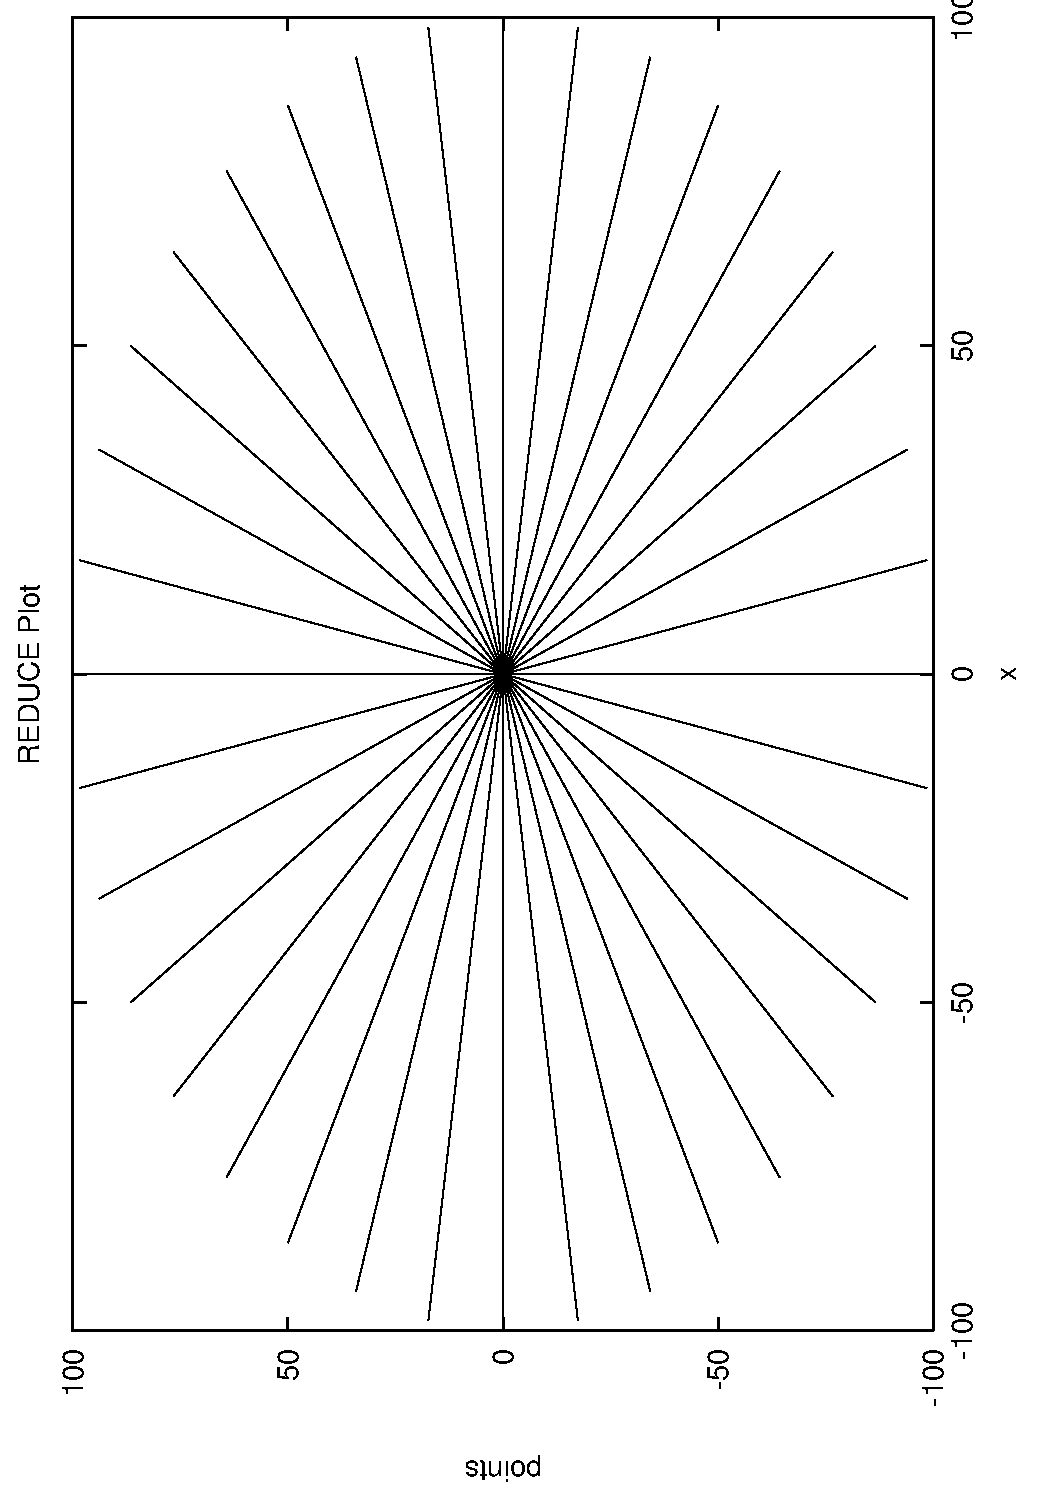
\includegraphics[bb=0 0 504 720,width=8cm,height=8cm,angle=270]{turtleeg1.pdf}}
\end{picture}

\begin{verbatim}
% (2) Draw 12 regular polygons with 12 sides of length 40,each polygon
%forming an angle of 360/n degrees with the previous one. 

draw {for i:=1:12 collect
          {leftturn(30), for j:=1:12 collect
                             {forward 40, leftturn(30)}} };
\end{verbatim}

\unitlength=1cm
\begin{picture}(8,8)(0,0)
\put (0,8){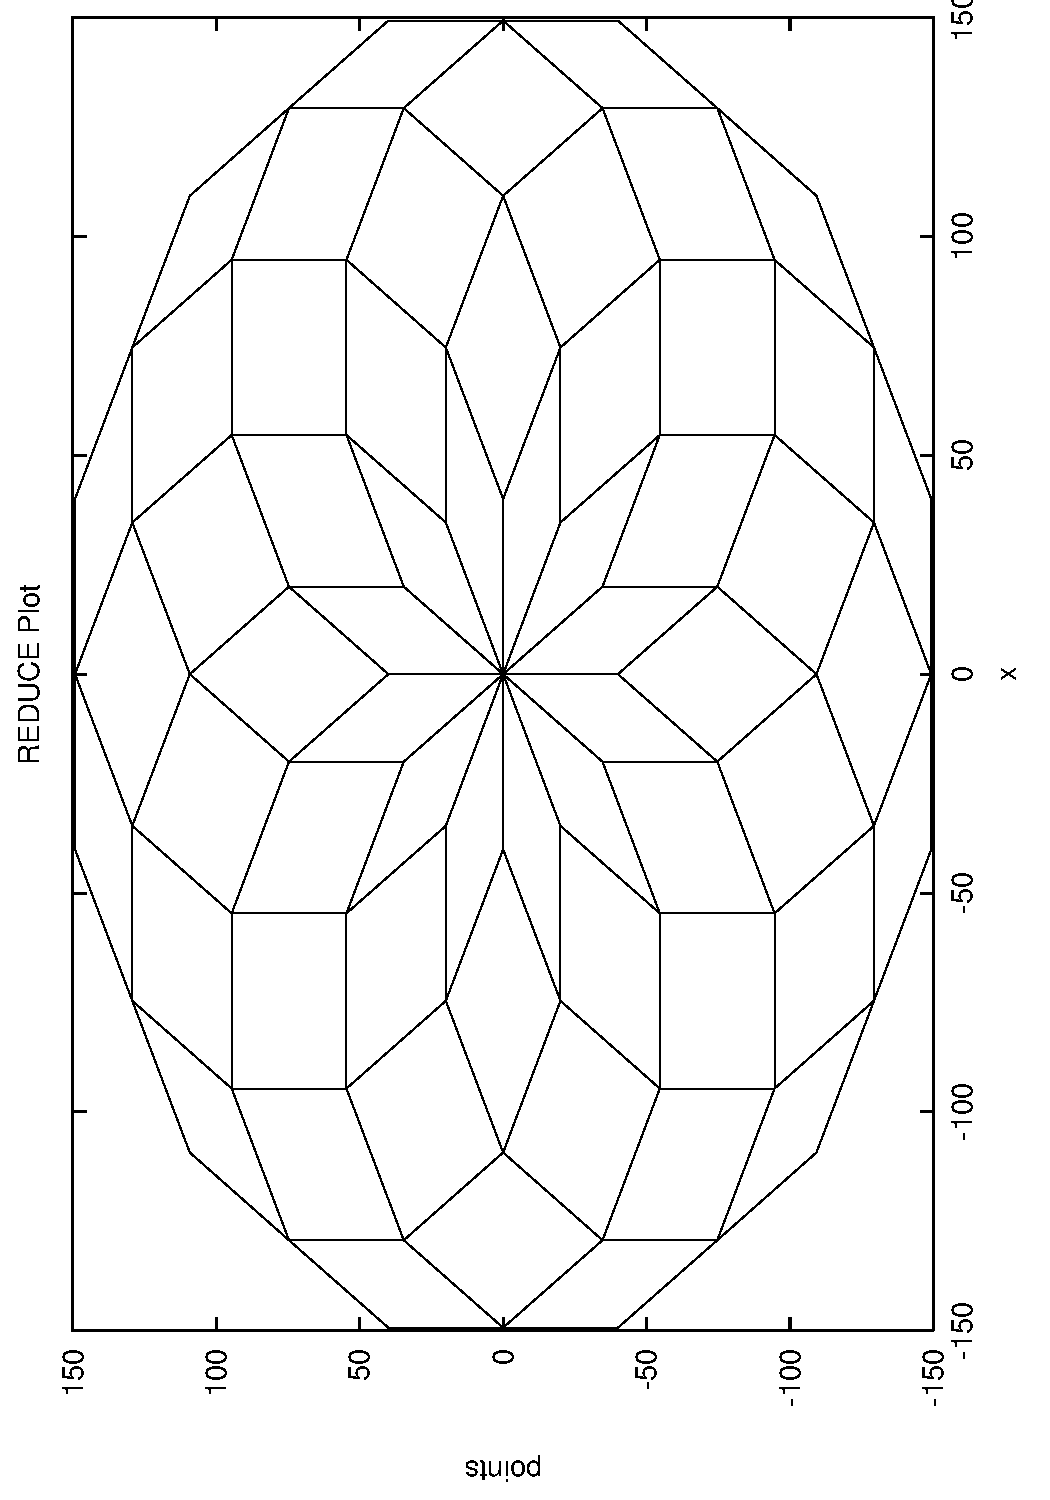
\includegraphics[bb=0 0 504 720,width=8cm,height=8cm,angle=270]{turtleeg4.pdf}}
\end{picture}

\begin{verbatim}
% (3) A "peak" pattern - an example of a recursive procedure.

procedure peak(r);
begin;
  return for i:=0:r collect
             {move(x_coord+5,y_coord-10), move(x_coord+10,y_coord+60),
              move(x_coord+10,y_coord-60),move(x_coord+5,y_coord+10)};
end;

draw {home(), peak(3)};
\end{verbatim}

\unitlength=1cm
\begin{picture}(8,8)(0,0)
\put (0,8){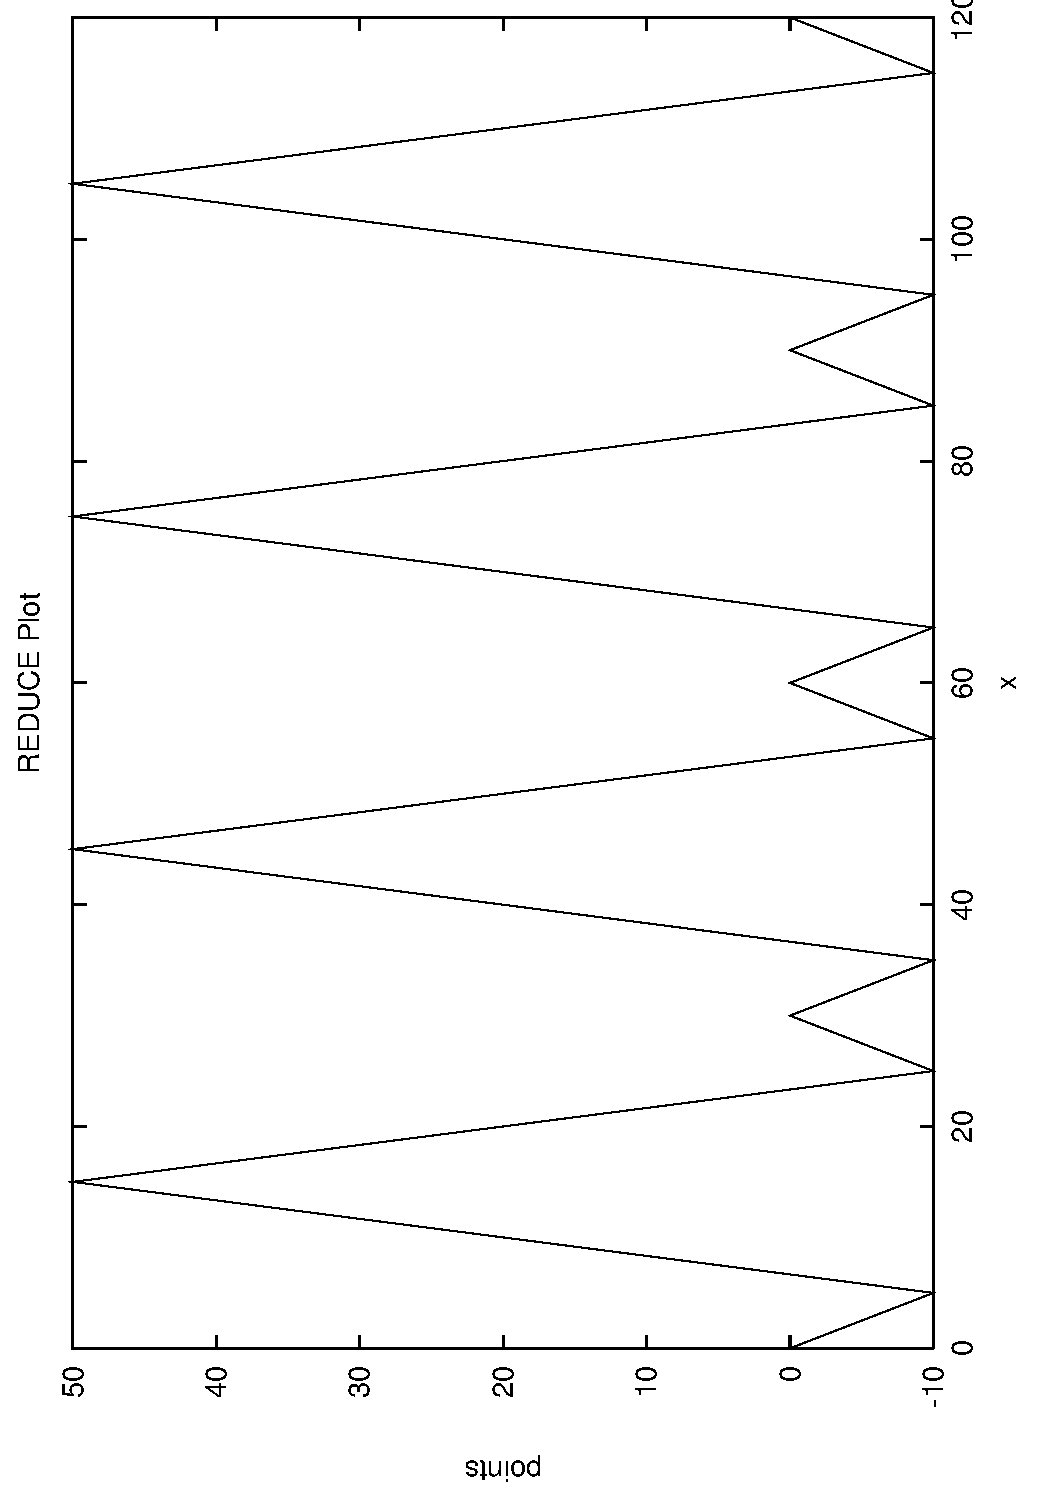
\includegraphics[bb=0 0 504 720,width=8cm,height=8cm,angle=270]{turtleeg5a.pdf}}
\end{picture}  

\begin{verbatim}
%This procedure can then be part of a longer chain of commands:

draw {home(), move(5,50), peak(3), move(x_coord+10,-100),
      peak(2), move(x_coord+10,0)};
\end{verbatim}

\unitlength=1cm
\begin{picture}(8,8)(0,0)
\put (0,8){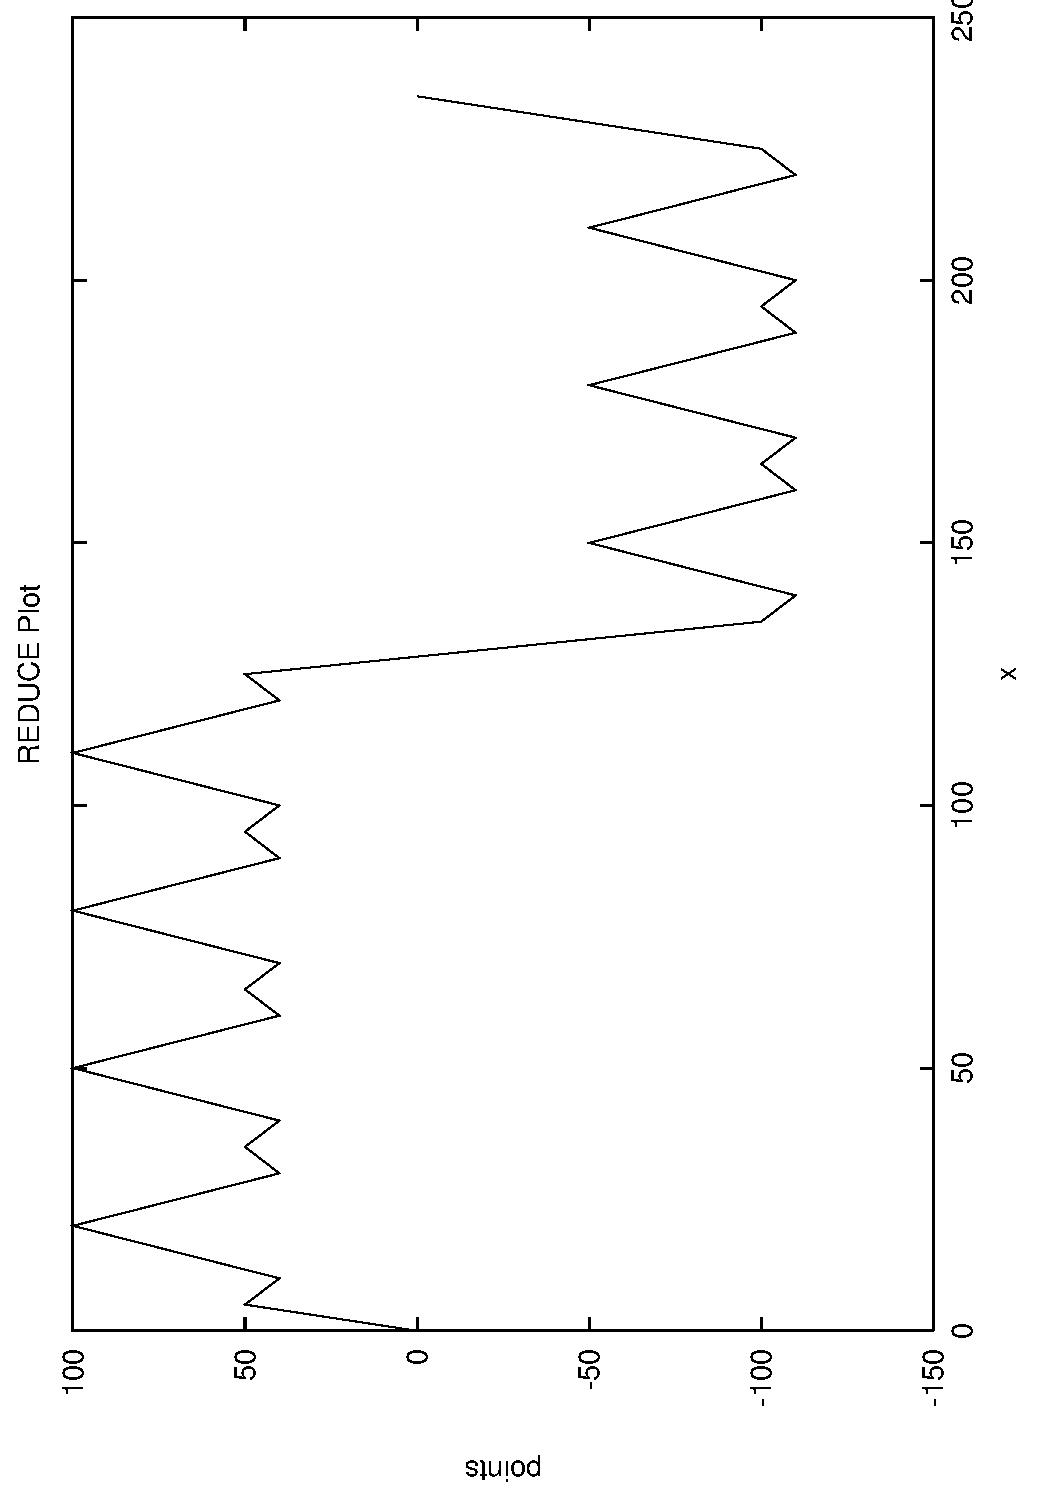
\includegraphics[bb=0 0 504 720,width=8cm,height=8cm,angle=270]{turtleeg5b.pdf}}
\end{picture}  

\begin{verbatim}
% (4)  Write a recursive procedure which draws "trees" such that every
%branch is half the length of the previous branch.

procedure tree(a,b);         %Here: a is the start length, b is the
                             %number of levels
begin;
  return if fixpb and b>0           %checking b is a positive integer

            then {leftturn(45), forward a, tree(a/2,b-1),
                  back a, rightturn(90), forward a, tree(a/2,b-1),
                  back a, leftturn(45)}
         else {x_coord,y_coord};    %default: Turtle stays still
end;

draw {home(), tree(130,7)};
\end{verbatim}

\unitlength=1cm
\begin{picture}(8,8)(0,0)
\put(0,8){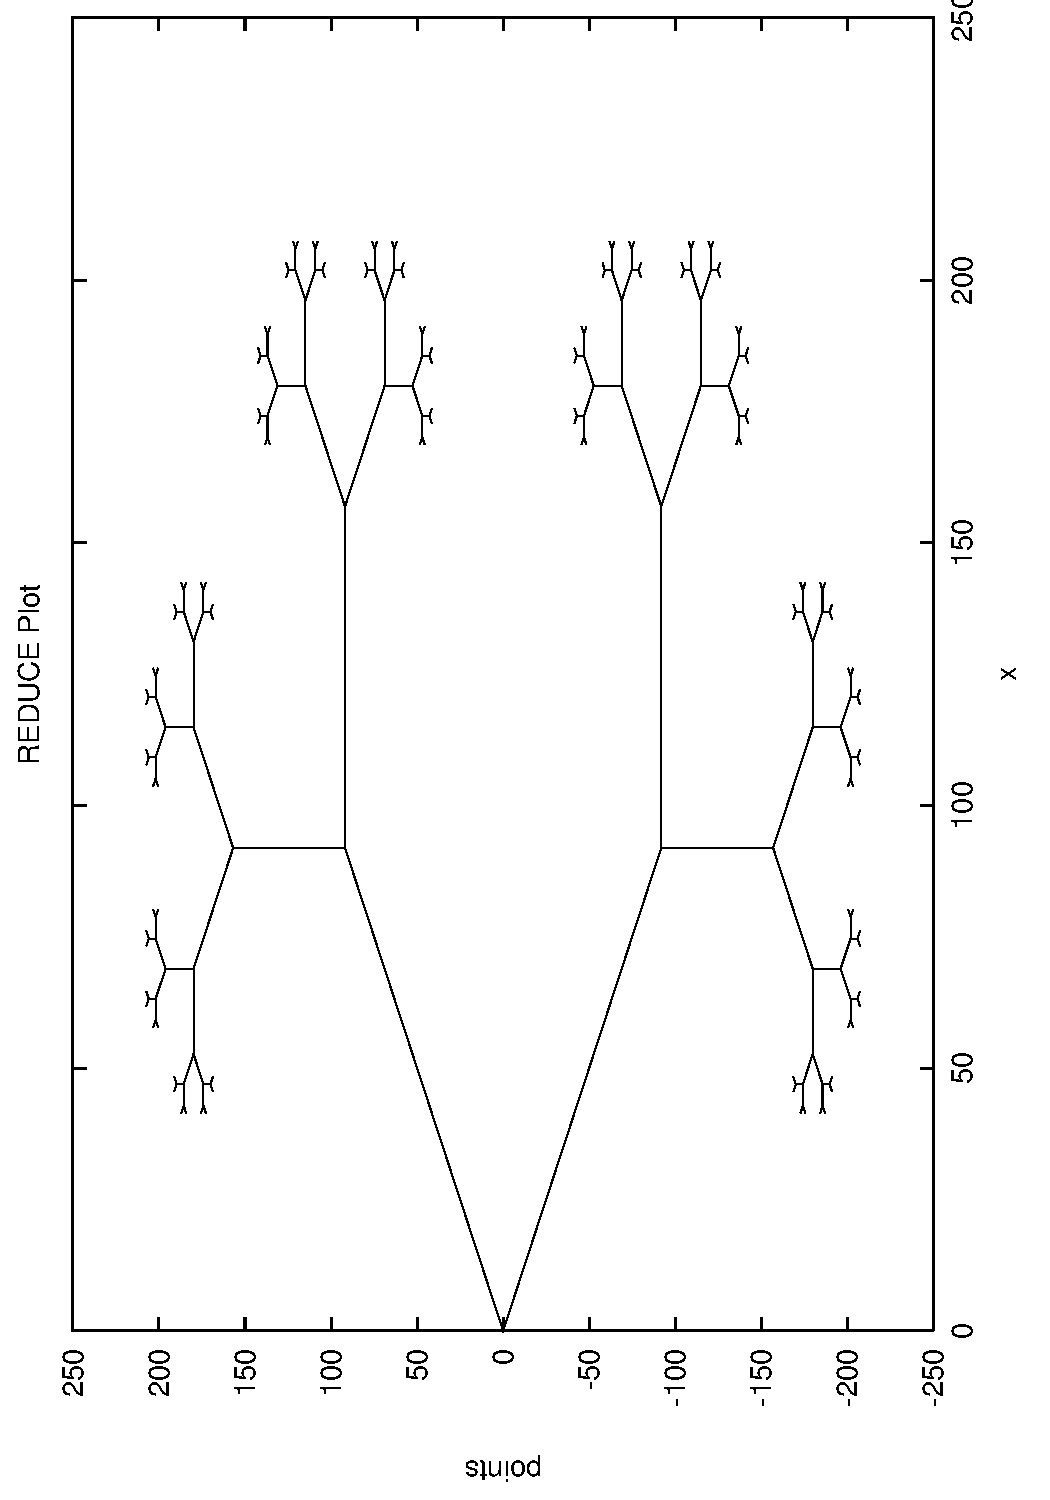
\includegraphics[bb=0 0 504 720,width=8cm,height=8cm,angle=270]{turtleeg6a.pdf}}
\end{picture}  

\begin{verbatim}
% (5)  A 36-point star.

draw {home(), for i:=1:36 collect
                  {leftturn(10), forward 100, leftturn(10), back 100} };
\end{verbatim}

\unitlength=1cm
\begin{picture}(8,8)(0,0)
\put(0,8){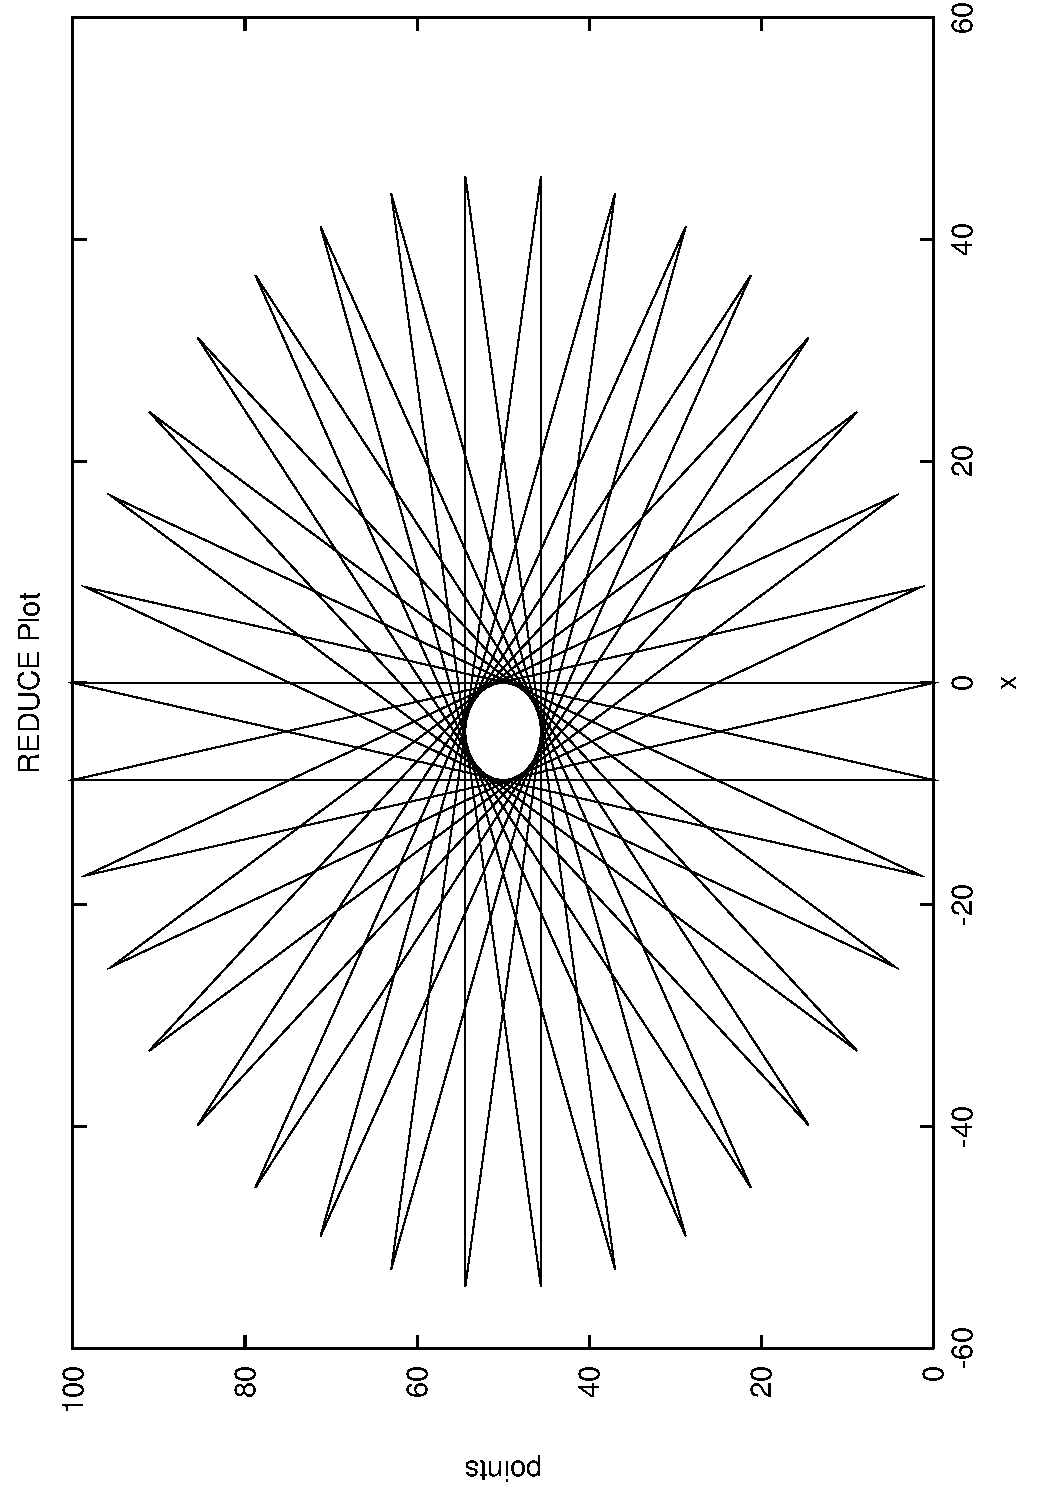
\includegraphics[bb=0 0 504 720,width=8cm,height=8cm,angle=270]{turtleeg7.pdf}}
\end{picture}  

\begin{verbatim}
% (6) Draw 100 equilateral triangles with the leading points
%equally spaced on a circular path.

draw {home(), for i:=1:100 collect
                  {forward 150, rightturn(60), back(150),
                   rightturn(60), forward 150, setheading(i*3.6)} };
\end{verbatim}

\unitlength=1cm
\begin{picture}(8,8)(0,0)
\put(0,8){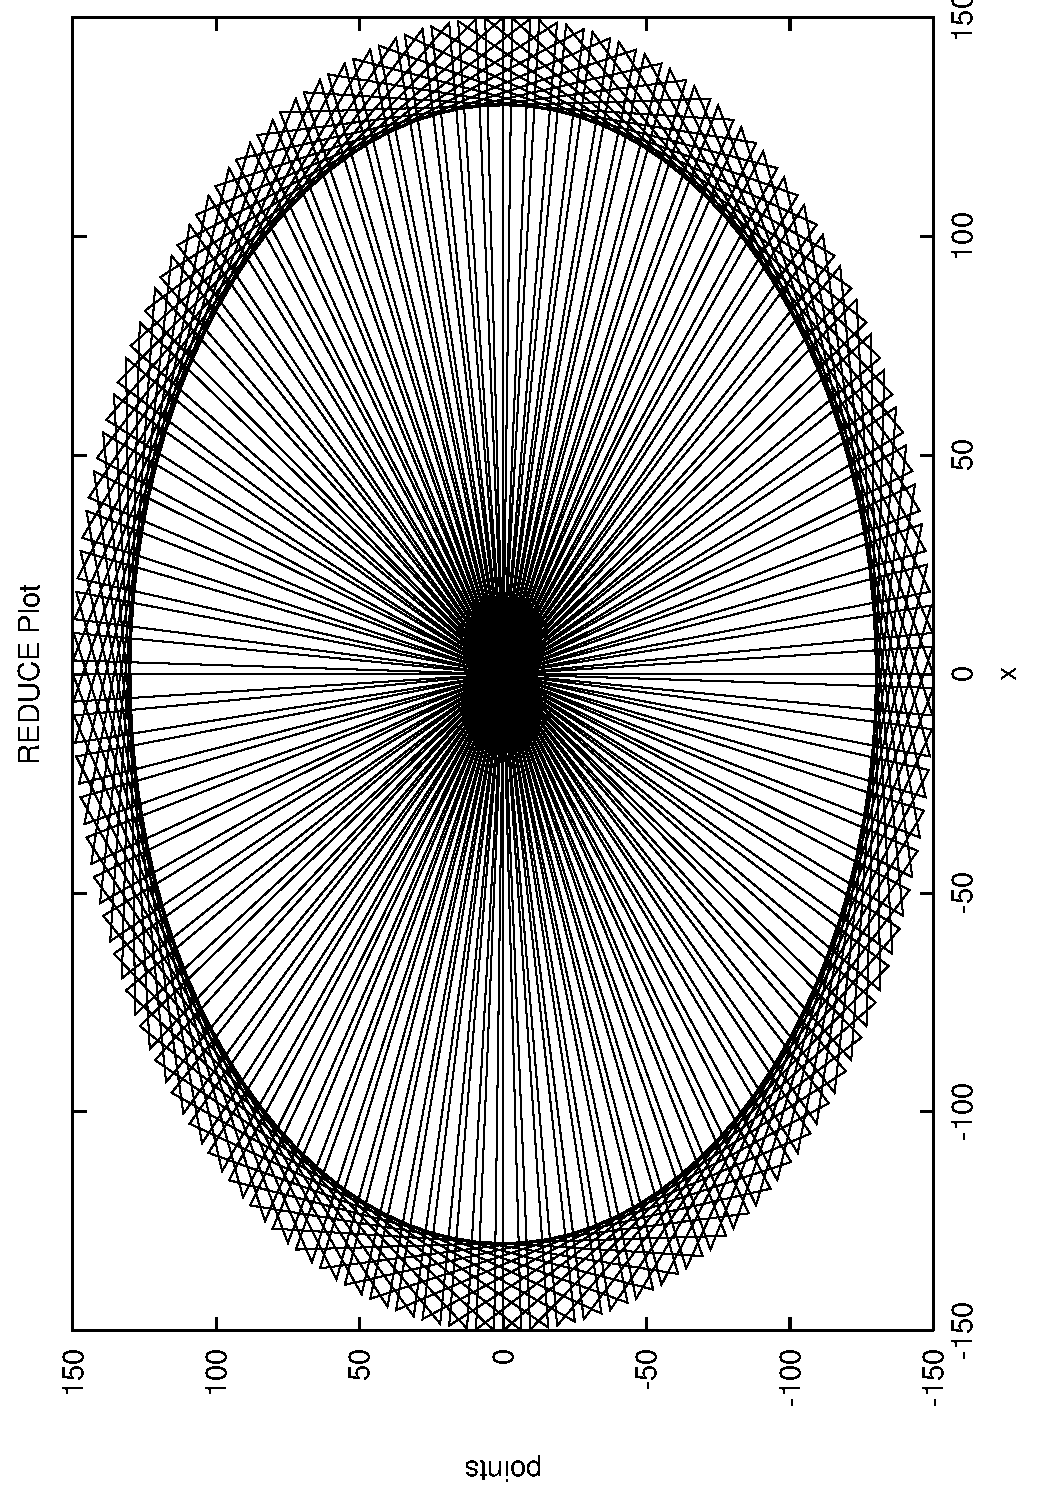
\includegraphics[bb=0 0 504 720,width=8cm,height=8cm,angle=270]{turtleeg8.pdf}}
\end{picture}  

\begin{verbatim}
% (7) Two or more graphs can be drawn together (this is easier
%if the graphs are named). Here we show graphs 2 and 6 on top of one
%another:

gr2:={home(), for i:=1:12 collect
                  {leftturn(30), for j:=1:12 collect
                                     {forward 40, leftturn(30)}} }$

gr6:={home(), for i:=1:100 collect
                  {forward 150, rightturn(60), back(150),
                   rightturn(60), forward 150, setheading(i*3.6)} }$

draw {gr2, gr6};
\end{verbatim}

\unitlength=1cm
\begin{picture}(8,8)(0,0)
\put(0,8){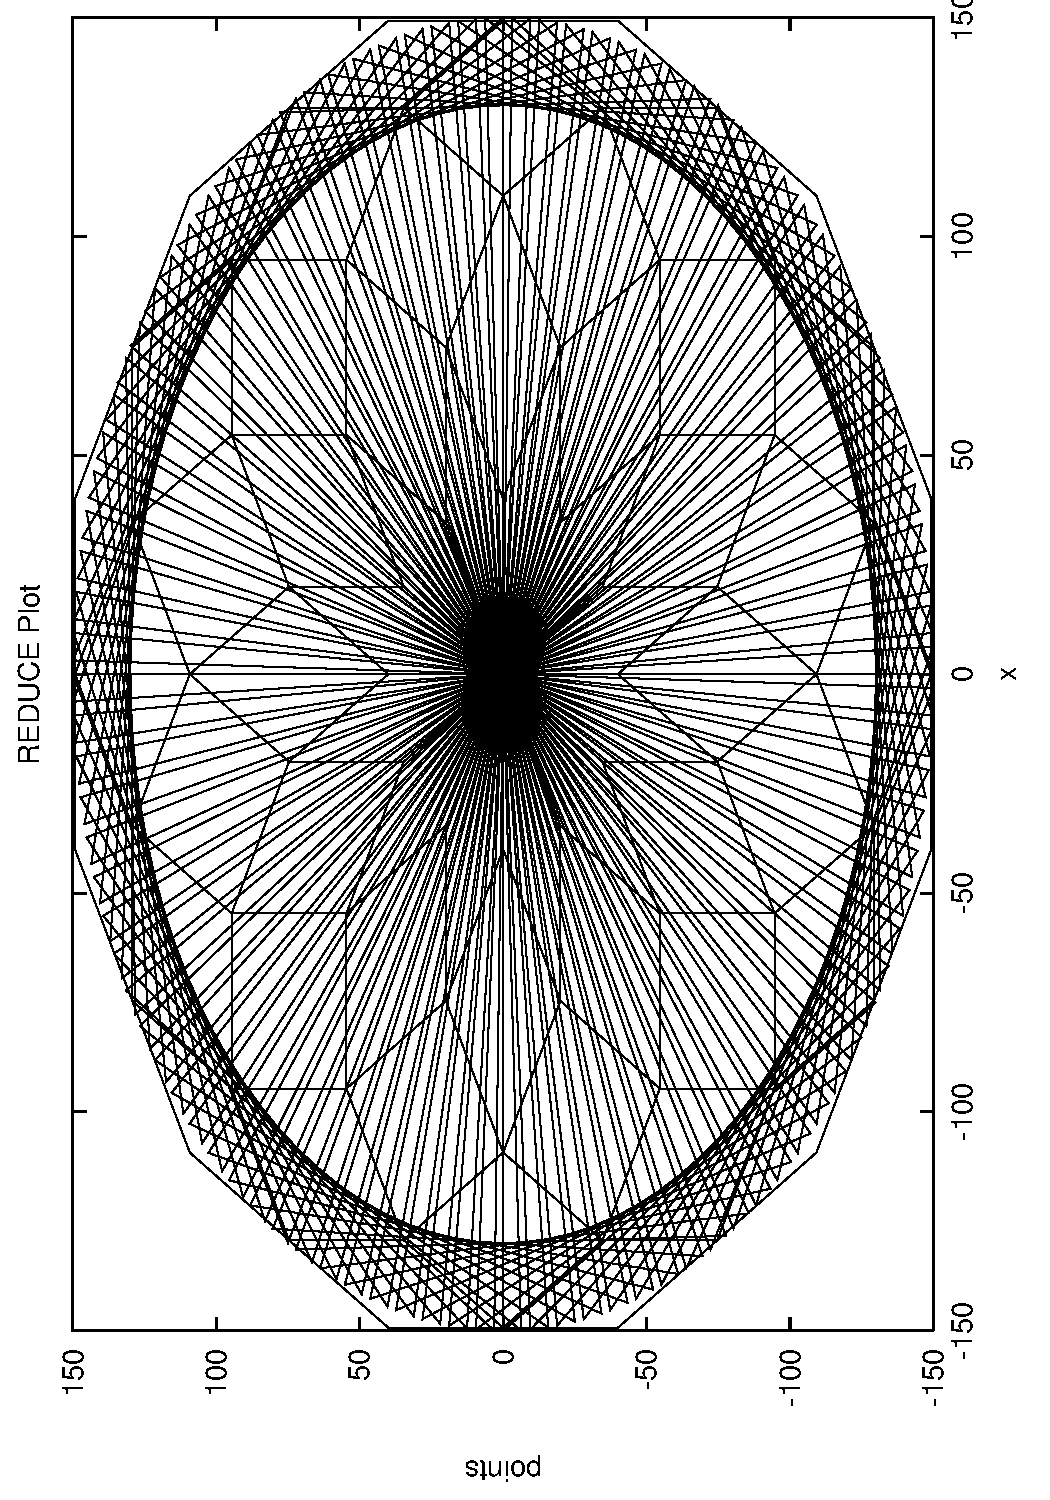
\includegraphics[bb=0 0 504 720,width=8cm,height=8cm,angle=270]{turtleeg9.pdf}}
\end{picture}  

\begin{verbatim}
% (8) Example 7 could have been tackled another way, which makes use of 
%the fdraw command.
%By inputting gr2 and gr6 as procedures into reduce, they can then be 
%used at any time in the same reduce session in a call to draw and even
%fdraw.

%First save the procedures in a file, say fxp (fdraw example procedures):

procedure gr2;
begin;
  return {home, for i:=1:12 collect
                    {leftturn(30), for j:=1:12 collect
                                       {forward 40, leftturn(30)}} };
end;

procedure gr6;
begin;
  return {home(), for i:=1:100 collect
                  {forward 150, rightturn(60), back(150),
                   rightturn(60), forward 150, setheading(i*3.6)} };
end;

%Then create another file where the functions may be called to fdraw,
%e.g. fx:

gr2
gr6

%Now in reduce, after loading the turtle package just type the following:

in "fxp";
fdraw '"fx";

%..and the graphs will appear.

%This method is useful if the user wants to define many of their own
%functions, and, using fdraw, subtle changes can be made quickly without 
%having to type out the whole string of commands to plot each time. It 
%is particularly useful if there are several pictures to plot at once and 
%it is an easy way to build pictures so that the difference an extra 
%command makes to the overall picture can be clearly seen.
%(In the above example, the file called to fdraw was only 2 lines long,
%so this method did not have any advantage over the normal draw command. 
%However, when the list of commands is longer it is clearly advantageous 
%to use fdraw)


\end{verbatim}


\subsection{References}

\begin{enumerate}
 \item {\bf An Implementation of Turtle Graphics for Teaching Purposes}\\
         Zoran I. Putnik \& Zoram d.Budimac

 \item {\bf Mapletech -} Maple in Mathematics and the Sciences,\\ 
        Special Issue 1994\\
       {\bf An Implementation of ``Turtle Graphics'' in Maple V}\\
         Eugenio Roanes Lozano \&  Eugenio Roanes Macias

\end{enumerate}






\newpage

\section{WU: Wu algorithm for polynomial systems}
\indexpackage{WU}

This is a simple implementation of the Wu algorithm implemented in REDUCE
working directly from ``A Zero Structure Theorem for
Polynomial-Equations-Solving,'' Wu Wen-tsun, Institute of Systems Science,
Academia Sinica, Beijing.

Author: Russell Bradford.

\documentstyle[fullpage]{article}

\pagestyle{empty}
\setlength{\parindent}{0in}
\setlength{\parskip}{0.1in}

\begin{document}
\title{An Implementation of the Wu Algorithm}
\author{Russell Bradford \\
School of Mathematical Sciences,\\
University of Bath,\\
Claverton Down,\\
Bath, BA2 7AY \\
\tt rjb@maths.bath.ac.uk}
\date{}
\maketitle\thispagestyle{empty}

This is a simple implementation of the Wu algorithm implemented in Reduce
3.3, working directly from
``A Zero Structure Theorem for Polynomial-Equations-Solving,''
Wu Wen-tsun, Institute of Systems Science, Academia Sinica, Beijing.

Its purpose was to aid my understanding of the algorithm, so the code is
simple, and has a lot of tracing included. This is a working implementation,
but there is magnificent scope for improvement and optimisation. Things
like using intelligent sorts on polynomial lists, and avoiding the
re-computation of various data spring easily to mind. Also, an attempt
at factorization of the input polynomials at each pass might have beneficial
results. Of course, exploitation of the natural parallel structure is a must!

All bug fixes and improvements are welcomed.

The interface:
\begin{verbatim}
wu( {x^2+y^2+z^2-r^2, x*y+z^2-1, x*y*z-x^2-y^2-z+1}, {x,y,z});
\end{verbatim}
calls {\tt wu} with the named polynomials, and with the variable ordering
${\tt x} > {\tt y} > {\tt z}$. In this example, {\tt r} is a parameter.

The result is
\begin{verbatim}
    2    3    2
{{{r  + z  - z  - 1,

    2  2    2      2    4    2  2    2
   r *y  + r *z + r  - y  - y *z  + z  - z - 2,

          2
   x*y + z  - 1},

  y},

    6  4      6  2    6      4  7      4  6      4  5      4  4
 {{r *z  - 2*r *z  + r  + 3*r *z  - 3*r *z  - 6*r *z  + 3*r *z  + 3*

    4  3      4  2      4      2  10      2  9      2  8      2  7
   r *z  + 3*r *z  - 3*r  + 3*r *z   - 6*r *z  - 3*r *z  + 6*r *z  +

       2  6      2  5      2  4      2  3      2    13      12    11
    3*r *z  + 6*r *z  - 6*r *z  - 6*r *z  + 3*r  + z   - 3*z   + z

         10    9      8      7    6      4      3    2
    + 2*z   + z  + 2*z  - 6*z  - z  + 2*z  + 3*z  - z  - 1,

    2   2    3    2
   y *(r  + z  - z  - 1),

          2
   x*y + z  - 1},

      2    3    2
  y*(r  + z  - z  - 1)}}
\end{verbatim}
namely, a list of pairs of characteristic sets and initials for the
characteristic sets.

Thus, the first pair above has the characteristic set
$$ r^2 + z^3 - z^2 - 1,
r^2 y^2 + r^2 z + r^2 - y^4 - y^2 z^2 + z^2 - z - 2,
x y + z^2 - 1$$
and initial $y$.

According to Wu's theorem, the set of roots of the original polynomials
is the union of the sets of roots of the characteristic sets,
with the additional constraints that the
corresponding initial is non-zero. Thus, for the first pair above, we find the
roots of $\{ r^2 + z^3 - z^2 - 1, \ldots~\}$ under the constraint that
$y \neq 0$. These roots, together with the roots of the other
characteristic set (under the constraint of $y(r^2+z^3-z^2-1) \neq 0$),
comprise all the roots of the original set.

Additional information about the working of the algorithm can be gained by
\begin{verbatim}
on trwu;
\end{verbatim}
This prints out details of the choice of basic sets, and the computation
of characteristic sets.

The second argument (the list of variables) may be omitted, when all the
variables in the input polynomials are implied with some random ordering.
\end{document}


\newpage

\section{XCOLOR: Color factor in some field theories}

\indexpackage{XCOLOR}

This package calculates the color factor in non-abelian gauge field
theories using an algorithm due to Cvitanovich.

Documentation for this package is in plain text.

Author: A. Kryukov.

\documentclass{article}

\usepackage[dvipdfm]{graphicx}
\usepackage[dvipdfm]{color}
\usepackage[dvipdfm]{hyperref}

\title{Program \char`\"{}xCOLOR\char`\"{}. User's Manual.}
\author{A.Kryukov \\
	Institute for Nuclear Physics \\
	Moscow State University \\
	119899, Moscow, RUSSIA \\
 	E-mail: kryukov@npi.msu.su \\
	Phone/Fax: (095) 939-0397}
\date{}

\setlength{\parindent}{0cm}

\begin{document}

\maketitle

\begin{abstract}
Program \char`\"{}xCOLOR\char`\"{} is intended for calculation the colour
factor in non-abelian gauge field theories. It is 
realized Cvitanovich algorithm {[}1{]}. In comparision with
\char`\"{}COLOR\char`\"{} program {[}2{]} it was made many improvements.
The package was writen by symbolic mode. This version is
faster then {[}2{]} more then 10 times.
\end{abstract} 

\ \\
After load the program by the following command \quad {\tt load xcolor}; \\
user can be able to use the next additional commands and operators. 

\subsubsection*{Command SUdim.}

Format: {\tt SUdim <any expression>}; \\
\ \\
Set the order of SU group. \\
\ \\
The default value is 3, i.e. SU(3). 

\subsubsection*{Command SpTT.}

Format: {\tt SpTT <any expression>}; \\
\ \\
Set the normalization coefficient A: Sp(TiTj) = A{*}Delta(i,j).
Default value is 1/2. 

\subsubsection*{Operator QG.}

Format: {\tt QG(inQuark,outQuark,Gluon)} \\
\ \\
Describe the quark-gluon vertex. Parameters may be any identifiers.
First and second of then must be in- and out- quarks correspondently.
Third one is a gluon. 

\subsubsection*{Operator G3.}

Format: {\tt G3(Gluon1,Gluon2,Gluon3)} \\
\ \\
Describe the three-gluon vertex. Parameters may be any identifiers.
The order of gluons must be clock. \\
\ \\
In terms of QG and G3 operators you input diagram in \char`\"{}color\char`\"{}
space as a product of these operators. For example. 

\begin{verbatim}


 Diagram:                       REDUCE expression:

            e1

         ---->---
        /        \
       |    e2    |
     v1*..........*v2  <===>  QG(e3,e1,e2)*QG(e1,e3,e2)
       |          |
        \   e3   /
         ----<---


Here: --->--- quark

      ....... gluon

\end{verbatim}

More detail see {[}2{]}. \\
\ \\
\ \\
\underline{References.} \\ 
\ \\
{[}1{]} P.Cvitanovic, Phys. Rev. D14(1976), p.1536.

{[}2{]} A.Kryukov \& A.Rodionov, Comp. Phys. Comm., 48(1988), pp.327-334.\\
\ \\
\ \\
\ \\
Please send any remarks to my address above! \\
\ \\
\ \\
Good luck!

\end{document}


\newpage

\section{XIDEAL: Gr\"obner Bases for exterior algebra}
\indexpackage{XIDEAL}
\label{package:XIDEAL}

XIDEAL constructs Gr\"obner bases for solving the left ideal membership
problem: Gr\"obner left ideal bases or GLIBs. For graded ideals, where each
form is homogeneous in degree, the distinction between left and right
ideals vanishes. Furthermore, if the generating forms are all homogeneous,
then the Gr\"obner bases for the non-graded and graded ideals are
identical. In this case, XIDEAL is able to save time by truncating the
Gr\"obner basis at some maximum degree if desired.

Author: David Hartley.


\subsection{Description}

The method of Gr{\"o}bner bases in commutative polynomial rings introduced by
Buchberger (e.g.~\cite{Buchberger:85}) is a well-known and very important tool
in polynomial ideal theory, for example in solving the ideal membership
problem. XIDEAL extends the method to exterior algebras using
algorithms from \cite{HartleyTuckey:93} and \cite{Apel:92}.

There are two main departures from the commutative polynomial case. First,
owing to the non-commutative product in exterior algebras, ideals are no
longer automatically two-sided, and it is necessary to distinguish between
left and right ideals. Secondly, because there are zero divisors, confluent
reduction relations are no longer sufficient to solve the ideal membership
problem: a unique normal form for every polynomial does not guarantee that
all elements in the ideal reduce to zero. This leads to two possible
definitions of Gr{\"o}bner bases as pointed out by Stokes \cite{Stokes:90}.

XIDEAL constructs Gr{\"o}bner bases for solving the left ideal membership
problem: Gr{\"o}bner left ideal bases or GLIBs. For graded ideals, where each
form is homogeneous in degree, the distinction between left and right
ideals vanishes. Furthermore, if the generating forms are all homogeneous,
then the Gr{\"o}bner bases for the non-graded and graded ideals are
identical. In this case, XIDEAL is able to save time by truncating the
Gr{\"o}bner basis at some maximum degree if desired.

XIDEAL uses the exterior calculus package EXCALC of E.~Schr{\"u}fer
\cite{Schruefer:85} to provide the exterior algebra definitions. EXCALC is loaded
automatically with XIDEAL.
% The basis 1-forms for the exterior algebra
% are automatically extracted from the input. Consequently, each expression
% must be written in terms of these 1-forms -- $p$-form kernels with $p>1$
% are not allowed. Similarly all distinct 1-forms in the input are assumed to
% be linearly independent -- if a dimension has been fixed (using the EXCALC
% \f{SPACEDIM} or \f{COFRAME} statements), then input containing more than this
% number of distinct 1-forms will generate an error. The exterior algebra can
% be based on either an abstract vector space or the cotangent space at some
% fixed point on a manifold. Any functions or 0-forms are treated as constant
% non-vanishing coefficients.
The exterior variables may be specified explicitly, or extracted
automatically from the input polynomials.  All distinct exterior variables
in the input are assumed to be linearly independent -- if a dimension has
been fixed (using the EXCALC \f{spacedim} or \f{coframe} statements), then
input containing distinct exterior variables with degrees totaling more
than this number will generate an error.

% The term ordering used is the graded lexicographical ordering based on the
% prevailing EXCALC kernel ordering for the basis 1-forms. This puts
% highest degree first and then sorts terms of the same degree
% lexicographically. The EXCALC kernel ordering can be changed with the
% \REDUCE{} \f{KORDER} or EXCALC \f{FORDER} statements.



\subsection{Declarations}


\subsubsection*{xorder}
\ttindex{XORDER}

\f{xorder} sets the term ordering for all other calculations. The syntax is
\begin{verbatim}
     xorder k
\end{verbatim}
where \f{k} is one of \f{lex}, \f{gradlex} or \f{deglex}. The
lexicographical ordering \f{lex} is based on the prevailing EXCALC kernel
ordering for the exterior variables. The EXCALC kernel ordering can be
changed with the \REDUCE{} \f{korder} or EXCALC \f{forder} declarations. The
graded lexicographical ordering \f{gradlex} puts terms with more factors
first (irrespective of their exterior degrees) and sorts terms of the same
grading lexicographically. The degree lexicographical ordering \f{deglex}
takes account of the exterior degree of the variables, putting highest
degree first and then sorting terms of the same degree lexicographically.
The default ordering is \f{deglex}.


\subsubsection*{xvars}
\ttindex{XVARS}

It is possible to consider scalar and 0-form variables in exterior
polynomials in two ways: as variables or as coefficient parameters. This
difference is crucial for Gr{\"o}bner basis calculations. By default, all
scalar variables which have been declared as 0-forms are treated as
exterior variables, along with any EXCALC kernels of degree 0. This
division can be changed with the \f{xvars} declaration. The syntax is
\begin{verbatim}
     xvars U,V,W,...
\end{verbatim}
where the arguments are either kernels or lists of kernels. All variables
specified in the \f{xvars} declaration are treated as exterior variables in
subsequent XIDEAL calculations with exterior polynomials, and any other
scalars are treated as parameters. This is true whether or not the
variables have been declared as 0-forms. The declaration
\begin{verbatim}
     xvars {}
\end{verbatim}
causes all degree 0 variables to be treated as parameters, and
\begin{verbatim}
     xvars nil
\end{verbatim}
restores the default. Of course, $p$-form kernels with $p\not=0$ are always
considered as exterior variables. The order of the variables in an
\f{xvars} declaration has no effect on the \REDUCE{} kernel ordering or
XIDEAL term ordering.



\subsection{Operators}


\subsubsection*{xideal}
\ttindex{XIDEAL}

\f{xideal} calculates a Gr{\"o}bner left ideal basis in
an exterior algebra. The syntax is
\begin{verbatim}
     xideal(S:list of forms[,V:list of kernels][,R:integer])
           :list of forms.
\end{verbatim}
\f{xideal} calculates a Gr{\"o}bner basis for the left ideal generated by
\f{S} using the current term ordering. The resulting list can be used for
subsequent reductions with \f{xmod} as long as the term ordering is not
changed. Which 0-form variables are to be regarded as exterior variables
can be specified in an optional argument \f{V} (just like an \f{xvars}
declaration). The order of variables in \f{V} has no effect on the term
ordering. If the set of generators \f{S} is graded, an optional parameter
\f{R} can be given, and \f{xideal} produces a truncated basis suitable for
reducing exterior forms of degree less than or equal to \f{R} in the left
ideal. This can save time and space with large problems, but the result
cannot be used for exterior forms of degree greater than \f{R}. The forms
returned by \f{xideal} are sorted in increasing order. See also the
switches \f{trxideal} and \f{xfullreduction}.


\subsubsection*{xmodideal}
\ttindex{XMODIDEAL}

\f{xmodideal} reduces exterior forms to their (unique) normal forms modulo
a left ideal. The syntax is
\begin{verbatim}
     xmodideal(F:form, S:list of forms):form
\end{verbatim}
or
\begin{verbatim}
     xmodideal(F:list of forms, S:list of forms)
              :list of forms.
\end{verbatim}
An alternative infix syntax is also available:
\begin{verbatim}
     F xmodideal S.
\end{verbatim}
\f{xmodideal(F,S)} first calculates a Gr{\"o}bner basis for the left ideal
generated by \f{S}, and then reduces \f{F}. \f{F} may be either a single
exterior form, or a list of forms, and \f{S} is a list of forms. If \f{F}
is a list of forms, each element is reduced, and any which vanish are
deleted from the result. 
% If this operator is used more than once, and \f{S} does not change
% between calls, then the Gr{\"o}bner basis is not recalculated. 
If the set of generators \f{S} is graded, then a truncated Gr{\"o}bner basis
is calculated using the degree of \f{F} (or the maximal degree in
\f{F}). See also \f{trxmod}.


\subsubsection*{xmod}
\ttindex{XMOD}

\f{xmod} reduces exterior forms to their (not necessarily unique) normal
forms modulo a set of exterior polynomials. The syntax is
\begin{verbatim}
     xmod(F:form, S:list of forms):form
\end{verbatim}
or
\begin{verbatim}
     xmod(F:list of forms, S:list of forms):list of forms.
\end{verbatim}
An alternative infix syntax is also available:
\begin{verbatim}
     F xmod S.
\end{verbatim}
\f{xmod(F,S)} reduces \f{F} with respect to the set of exterior polynomials
\f{S}, which is not necessarily a Gr{\"o}bner basis. \f{F} may be either a
single exterior form, or a list of forms, and \f{S} is a list of
forms. This operator can be used in conjunction with \f{xideal} to produce
the same effect as \f{xmodideal}: for a single homogeneous form \f{F} and a
set of exterior forms \f{S}, \f{F xmodideal S} is equivalent to \f{F xmod
xideal(S,exdegree F)}. See also \f{trxmod}.


\subsubsection*{xauto}
\ttindex{XAUTO}

\f{xauto} autoreduces a set of exterior forms. The syntax is
\begin{verbatim}
     xauto(S:list of forms):list of forms.
\end{verbatim}
\f{xauto S} returns a set of exterior polynomials which generate the same
left ideal, but which are in normal form with respect to each other. For
linear expressions, this is equivalent to finding the reduced row echelon
form of the coefficient matrix.


\subsubsection*{excoeffs}
\ttindex{EXCOEFFS}

The operator \f{excoeffs}, with syntax
\begin{verbatim}
     excoeffs(F:form):list of expressions
\end{verbatim}
returns the coefficients from an exterior form as a list. The coefficients
are always scalars, but which degree 0 variables count as coefficient
parameters is controlled by the command \f{xvars}.


\subsubsection*{exvars}
\ttindex{EXVARS}

The operator \f{exvars}, with syntax
\begin{verbatim}
     exvars(F:form):list of kernels
\end{verbatim}
returns the exterior powers from an exterior form as a list. All non-scalar
variables are returned, but which degree 0 variables count as coefficient
parameters is controlled by the command \f{xvars}.


\subsection{Switches} 


\subsubsection*{xfullreduce}
\ttindextype{XFULLREDUCE}{switch}

\f{on xfullreduce} allows \f{xideal} and \f{xmodideal} to calculate
reduced, monic Gr{\"o}bner bases, which speeds up subsequent reductions, and
guarantees a unique form for the Gr{\"o}bner basis. \f{off xfullreduce} turns
of this feature, which may speed up calculation of some Gr{\"o}bner
basis. \f{xfullreduce} is \f{on} by default.


\subsubsection*{trxideal}
\ttindextype{TRXIDEAL}{switch}

\f{on trxideal} produces a trace of the calculations done by \f{xideal} and
\f{xmodideal}, showing the basis polynomials and the results of the
critical element calculations. This can generate profuse amounts of output.
\f{trxideal} is \f{off} by default.


\subsubsection*{trxmod}
\ttindextype{TRXMOD}{switch}

\f{on trxmod} produces a trace of reductions to normal form during
calculations by XIDEAL operators. \f{trxmod} is \f{off} by default.


% \subsubsection*{XSTATS}

% \f{ON XSTATS} produces counting and timing information. As \f{XIDEAL} is
% running, a hash mark (\verb.#.) is printed for each form taken from the
% input list, followed by a sequences of carets (\verb.^.) and dollar signs
% (\verb.$.). Each caret represents a new basis element obtained by a simple
% wedge product, and each dollar sign represents a new basis element obtained
% from an S-polynomial. At the end, a table is printed summarising the
% calculation. \f{XSTATS} is \f{OFF} by default.

\subsection{Examples}

Suppose XIDEAL has been loaded, the switches are at their default settings,
and the following exterior variables have been declared:

\begin{verbatim}
     pform x=0,y=0,z=0,t=0,f(i)=1,h=0,hx=0,ht=0;
\end{verbatim}

In a commutative polynomial ring, a single polynomial is its own Gr{\"o}bner
basis. This is no longer true for exterior algebras because of the presence
of zero divisors, and can lead to some surprising reductions:
\begin{verbatim}
     xideal {d x^d y - d z^d t};

          {d t^d z + d x^d y,

           d x^d y^d z,

           d t^d x^d y}

     f(3)^f(4)^f(5)^f(6) 
       xmodideal {f(1)^f(2) + f(3)^f(4) + f(5)^f(6)};

          0
\end{verbatim}

The heat equation, $h_{xx}=h_t$ can be represented by the following
exterior differential system. 
\begin{verbatim}
     S := {d h - ht*d t - hx*d x,
           d ht^d t + d hx^d x,
           d hx^d t - ht*d x^d t};
\end{verbatim}
\f{xmodideal} can be used to check that the exterior differential system is
closed under exterior differentiation.
\begin{verbatim}
     d S xmodideal S;

          {}
\end{verbatim}

\f{xvars}, or a second argument to \f{xideal} can be used to change the
division between exterior variables of degree 0 and parameters.
\begin{verbatim}
        xideal {a*d x+y*d y};

                  d x*a + d y*y
                {---------------}
                        a

        xvars {a};
        xideal {a*d x+y*d y};
 
                {d x*a + d y*y,d x^d y}
 
        xideal({a*d x+y*d y},{a,y});
 
                {d x*a + d y*y,
 
                 d x^d y*y}
 
        xvars {};       % all 0-forms are coefficients
        excoeffs(d u - (a*p - q)*d y);
        
                {1, - a*p + q}
        
        exvars(d u - (a*p - q)*d y);

                {d u,d y}

        xvars {p,q};    % p,q are no longer coefficients
        excoeffs(d u - (a*p - q)*d y);
        
                { - a,1,1}

        exvars(d u - (a*p - q)*d y);

                {d y*p,d y*q,d u}

        xvars nil;
\end{verbatim}


Non-graded left and right ideals are no longer the same:
\begin{verbatim}
     d t^(d z+d x^d y) xmodideal {d z+d x^d y};

          0

     (d z+d x^d y)^d t xmodideal {d z+d x^d y};

           - 2*d t^d z
\end{verbatim}
Any form containing a 0-form term generates the whole ideal:
\begin{verbatim}
     xideal {1 + f(1) + f(1)^f(2) + f(2)^f(3)^f(4)};

          {1}
\end{verbatim}



\newpage

\section{ZEILBERG: Indefinite and definite summation}

\indexpackage{ZEILBERG}

This package is a careful implementation of the Gosper and Zeilberger
algorithms for indefinite and definite summation of hypergeometric terms,
respectively.  Extensions of these algorithms are also included that are
valid for ratios of products of powers, factorials, $\Gamma$ function
terms, binomial coefficients, and shifted factorials that are
rational-linear in their arguments.

Authors: Gregor St\"olting and Wolfram Koepf.


\newcommand{\funkdef}[3]{\left\{\begin{array}{cc}
                                #1 & \mbox{\rm{if} $#2$ } \\
                                #3 & \mbox{\rm{otherwise}}
                                \end{array}\right.}

\subsection{Introduction}

%% For MathJax, must be part of a paragraph to avoid extra space:
\ifdefined\HCode
\(
\def\funkdef#1#2#3{\left\{\begin{array}{cc}
                                #1 & \textrm{if } #2 \\
                                #3 & \textrm{otherwise}
                          \end{array}\right.}
\)%
\fi
This package is a careful implementation of the Gosper%
\footnote{The {\tt sum} package contains also a partial implementation
of the Gosper algorithm.}
and Zeilberger algorithms for indefinite, and definite summation of
hypergeometric terms, respectively. Further, extensions of these algorithms
given by the first author are covered. An expression $a_k$ is called a
\textsl{hypergeometric term} (or \textsl{closed form}),
if $a_{k}/a_{k-1}$ is a rational function with respect to $k$.
Typical hypergeometric terms are ratios of products of powers, factorials,
$\Gamma$ function terms, binomial coefficients, and shifted factorials
(Pochhammer symbols) that are integer-linear in their arguments.

The extensions of Gosper's and Zeilberger's algorithm mentioned
in particular are valid for ratios of products of powers, factorials,
$\Gamma$ function terms, binomial coefficients, and shifted factorials
that are rational-linear in their arguments.

\subsection{Gosper Algorithm}

The Gosper algorithm \cite{Gosper:78} is a \textsl{decision procedure}, that
decides by algebraic calculations whether or not a given hypergeometric term
$a_k$ has a hypergeometric term antidifference $g_k$, i.\ e.\
$g_{k}-g_{k-1}=a_k$ with rational $g_k/g_{k-1}$,
and returns $g_k$ if the procedure is successful, in which
case we call $a_k$ \textsl{Gosper-summable}. Otherwise
\textsl{no hypergeometric term antidifference exists}. Therefore
if the Gosper algorithm does not return a closed form solution,
it has \textsl{proved} that no such solution exists, an information
that may be quite useful and important.
The Gosper algorithm is the discrete analogue of the Risch algorithm
for integration in terms of elementary functions.

Any antidifference is uniquely determined up to a constant, and is
denoted by
\[
g_k=\sum\nolimits_k a_k
\;.
\]
Finding $g_k$ given $a_k$ is called \textsl{indefinite summation}.
The antidifference operator $\Sigma$ is the inverse of the downward
difference operator $\nabla a_k=a_{k}-a_{k-1}$. There is an analogous
summation theory corresponding to the upward difference operator
$\Delta a_k=a_{k+1}-a_k$.

In case, an antidifference $g_k$ of $a_k$ is known, any sum
\[
\sum_{k=m}^{n} a_k=g_{n}-g_{m-1}
\]
can be easily calculated by an evaluation of $g$ at the boundary points
like in the integration case. Note, however, that the sum
\begin{equation}
\sum_{k=0}^n \binom{n}{k}
\label{eq:nchoosek}
\end{equation}
e.\ g.\
is not of this type since the summand $\binom{n}{k}$ depends on the upper
boundary point $n$ explicitly. This is an example of a definite sum
that we consider in the next section.

Our package supports the input of powers ({\tt a\verb+^+k)},
factorials ({\tt factorial(k)}),
$\Gamma$ function terms ({\tt gamma(a)}), binomial coefficients
({\tt binomial(n,k)}), shifted factorials
({\tt pochhammer(a,k)$=a(a+1)\cdots(a+k-1)=\Gamma (a+k)/\Gamma (a)$}), and
partially products ({\tt prod(f,k,k1,k2)}).
It takes care of the necessary simplifications, and therefore
provides you with the solution of the decision problem
as long as the memory or time requirements are not too high for the
computer used.

\subsection{Zeilberger Algorithm}

The (fast) Zeilberger algorithm \cite{Zeilberger:90}--\cite{Zeilberger:91}
deals with the \textsl{definite summation} of
hypergeometric terms. Zeilberger's paradigm is to find (and return)
a linear homogeneous recurrence equation with polynomial coefficients
(called \textsl{holonomic equation}) for an \textsl{infinite sum}
\[
s(n)=\sum_{k=-\infty}^{\infty} f(n,k)
\;,
\]
the summation to be understood over all integers $k$,
if $f(n,k)$ is a hypergeometric term with respect to both $k$ and $n$.
The existence of a holonomic recurrence equation for $s(n)$ is then
generally guaranteed.

If one is lucky, and the resulting recurrence equation is of first order
\[
p(n)\,s(n-1)+q(n)\,s(n)=0
\quad\quad(p,q\;\mbox{polynomials})
\;,
\]
$s(n)$ turns out to be a hypergeometric term, and a closed form solution
can be easily established using a suitable initial value, and is
represented by a ratio of Pochhammer or $\Gamma$ function terms if the
polynomials $p$, and $q$ can be factored.

Zeilberger's algorithm does not guarantee to find the holonomic equation
of lowest order, but often it does.

If the resulting recurrence equation has order larger than one,
this information can be used for identification purposes:
Any other expression satisfying the same recurrence equation, and the same
initial values, represents the same function.

Note that a \textsl{definite sum} $\sum\limits_{k=m_1}^{m_2} f(n,k)$ is an
infinite sum if $f(n,k)=0$ for $k<m_1$ and $k>m_2$.
This is often the case, an example of which is the sum (\ref{eq:nchoosek})
considered above, for which the hypergeometric recurrence equation
$2 s(n-1) - s(n) = 0$ is generated by Zeilberger's algorithm, leading
to the closed form solution $s(n)=2^n$.

Definite summation is trivial if the corresponding indefinite sum
is Gosper-summable analogously to the fact that definite integration
is trivial as soon as an elementary antiderivative is known.  If this is
not the case, the situation is much more difficult, and it is therefore
quite remarkable and non-obvious
that Zeilberger's method is just a clever application of Gosper's algorithm.

Our implementation is mainly based on \cite{Koornwinder:93} and \cite{Koepf:94b}.
More examples can be found in \cite{PauleSchorn:95}, \cite{Strehl:93}, \cite{Wilf:90},
and \cite{Wilf:93} many of which are contained in the test file
{\tt zeilberg.tst}.

\subsection{\REDUCE{} operator {\tt GOSPER}}

The ZEILBERG package must be loaded by:

{\small
\begin{verbatim}
1: load zeilberg;
\end{verbatim}
}\noindent
The \texttt{gosper} operator\ttindex{GOSPER} is an implementation of the Gosper algorithm.
\begin{itemize}
\item
{\tt gosper(a,k)} determines a closed
form antidifference. If it does not return a closed form solution, then
a closed form solution does not exist.
\item
{\tt gosper(a,k,m,n)} determines
\[
\sum_{k=m}^n a_k
\]
using Gosper's algorithm. This is only successful if Gosper's algorithm applies.
\end{itemize}

Example:

{\small
\begin{verbatim}
2: gosper((-1)^(k+1)*(4*k+1)*factorial(2*k)/
   (factorial(k)*4^k*(2*k-1)*factorial(k+1)),k);

              k
      - ( - 1) *factorial(2*k)
------------------------------------
  2*k
 2   *factorial(k + 1)*factorial(k)
\end{verbatim}
}\noindent
This solves a problem given in SIAM Review (\cite{OverhauserKim:94}, Problem 94--2)
where it was asked to determine the infinite sum
\[
S=\lim_{n\rightarrow\infty} S_n
\;,
\quad\quad\quad
S_n=\sum_{k=1}^n
\frac{(-1)^{k+1}(4k+1)(2k-1)!!}{2^k(2k-1)(k+1)!}
\;,
\]
($(2k-1)!!=1\cdot 3 \cdots (2k-1)=\frac{(2k)!}{2^k\,k!}$).
The above calculation shows that the summand is Gosper-summable,
and the limit $S=1$ is easily established using Stirling's formula.

The implementation solves further deep and difficult problems some examples of
which are:%

{\small
\begin{verbatim}
3:  gosper(sub(n=n+1,binomial(n,k)^2/binomial(2*n,n))-
    binomial(n,k)^2/binomial(2*n,n),k);

                   2
((binomial(n + 1,k) *binomial(2*n,n)

                                            2
   - binomial(2*(n + 1),n + 1)*binomial(n,k) )*(2*k - 3*n - 1)

             2                                       3      2
 *(k - n - 1) )/((2*(2*(n + 1) - k)*(2*n + 1)*k - 3*n  - 7*n  - 5*n

                     - 1)*binomial(2*(n + 1),n + 1)*binomial(2*n,n))

4: gosper(binomial(k,n),k);

 (k + 1)*binomial(k,n)
-----------------------
         n + 1

5: gosper((-25+15*k+18*k^2-2*k^3-k^4)/
   (-23+479*k+613*k^2+137*k^3+53*k^4+5*k^5+k^6),k);

          2
    - (2*k  - 15*k + 8)*k
----------------------------
      3      2
 23*(k  + 4*k  + 27*k + 23)
\end{verbatim}
}\noindent
The Gosper algorithm is not capable to give antidifferences depending
on the harmonic numbers
\[
H_k:=\sum_{j=1}^k\frac{1}{j}
\;,
\]
e.\ g.\ $\sum_k H_k=(k+1)(H_{k+1}-1)$, but, is able to give a proof, instead,
for the fact that $H_k$ does not possess a closed form evaluation:

{\small
\begin{verbatim}
6: gosper(1/k,k);

***** Gosper algorithm: no closed form solution exists
\end{verbatim}
}\noindent
The following code gives the solution to a summation problem proposed in
Gosper's original paper \cite{Gosper:78}. Let
\[
f_k=\prod_{j=1}^k (a+b\,j+c\,j^2)
\quad\quad\mbox{and}\quad\quad
g_k=\prod_{j=1}^k (e+b\,j+c\,j^2)
\;.
\]
Then a closed form solution for
\[
\sum\nolimits_k\frac{f_{k-1}}{g_{k}}
\]
is found by the definitions

{\small
\begin{verbatim}
7: operator ff,gg$

8: let {ff(~k+~m) => ff(k+m-1)*(c*(k+m)^2+b*(k+m)+a)
        when (fixp(m) and m>0),
   ff(~k+~m) => ff(k+m+1)/(c*(k+m+1)^2+b*(k+m+1)+a)
        when (fixp(m) and m<0)}$

9: let {gg(~k+~m) => gg(k+m-1)*(c*(k+m)^2+b*(k+m)+e)
        when (fixp(m) and m>0),
   gg(~k+~m) => gg(k+m+1)/(c*(k+m+1)^2+b*(k+m+1)+e)
        when (fixp(m) and m<0)}$
\end{verbatim}
}\noindent
and the calculation

{\small
\begin{verbatim}
10: gosper(ff(k-1)/gg(k),k);

     ff(k)
---------------
 (a - e)*gg(k)

11: clear ff,gg$
\end{verbatim}
}\noindent
Similarly closed form solutions of $\sum\nolimits_k\frac{f_{k-m}}{g_{k}}$
for positive integers $m$ can be obtained, as well as of
$\sum_k\frac{f_{k-1}}{g_{k}}$ for
\[
f_k=\prod_{j=1}^k (a+b\,j+c\,j^2+d\,j^3)
\quad\quad\mbox{and}\quad\quad
g_k=\prod_{j=1}^k (e+b\,j+c\,j^2+d\,j^3)
\]
and for analogous expressions of higher degree polynomials.

\subsection{\REDUCE{} operator {\tt EXTENDED\_GOSPER}}
\ttindex{EXTENDED\_GOSPER}
The {\tt extended\_gosper} operator is an implementation of an extended
version of Gosper's algorithm given by Koepf \cite{Koepf:94b}.
\begin{itemize}
\item
{\tt extended\_gosper(a,k)} determines an antidifference $g_k$ of $a_k$
whenever there is a number $m$ such that $h_{k}-h_{k-m}=a_k$, and $h_k$ is an
\textsl{$m$-fold hypergeometric term}, i.\ e.
\[
h_{k}/h_{k-m}\quad\mbox{is a rational function with respect to $k$.}
\]
If it does not return a solution, then such a solution does not exist.
\item
{\tt extended\_gosper(a,k,m)}
determines an \textsl{$m$-fold antidifference} $h_k$ of $a_k$,
i.\ e.\ $h_{k}-h_{k-m}=a_k$, if it is an $m$-fold hypergeometric term.
\end{itemize}
Examples:

{\small
\begin{verbatim}
12: extended_gosper(binomial(k/2,n),k);

                   k                         k - 1
 (k + 2)*binomial(---,n) + (k + 1)*binomial(-------,n)
                   2                           2
-------------------------------------------------------
                       2*(n + 1)

13: extended_gosper(k*factorial(k/7),k,7);

                   k
(k + 7)*factorial(---)
                   7
\end{verbatim}
}\noindent

\subsection{\REDUCE{} operator {\tt SUMRECURSION}}
\ttindex{SUMRECURSION}

The {\tt sumrecursion} operator is an implementation of the (fast)
Zeilberger algorithm.
\begin{itemize}
\item
{\tt sumrecursion(f,k,n)} determines a holonomic recurrence equation
for
\[
{\tt sum(n)} =\sum\limits_{k=-\infty}^\infty f(n,k)
\]
with respect to $n$, applying
{\tt extended\_sumrecursion} if necessary,
see \S~\ref{sec:EXTENDED_SUMRECURSION}.
The resulting expression equals zero.
\item
{\tt sumrecursion(f,k,n,j)} % $(j\in\mathbb{N})$
searches for a holonomic recurrence equation of order $j$. This
operator does not use {\tt extended\_sumrecursion} automatically.
Note that if $j$ is too large, the recurrence equation
may not be unique, and only one particular solution is returned.
\end{itemize}
A simple example deals with Equation (\ref{eq:nchoosek})%
\footnote{Note that with \REDUCE{} Version 3.5 we use the global operator
{\tt summ} instead of {\tt sum} to denote the sum.}

{\small
\begin{verbatim}
14: sumrecursion(binomial(n,k),k,n);

2*sum(n - 1) - sum(n)
\end{verbatim}
}\noindent
The whole \textsl{hypergeometric database} of the {\sl
Vandermonde, Gau{\ss}, Kummer, Saalsch\"utz, Dixon, Clausen} and \textsl{Dougall
identities} (see \cite{Wilf:93}), and many more identities (see e.\ g.\
\cite{Koepf:94b}), can be obtained using {\tt sumrecursion}.
As examples, we consider the difficult cases of Clausen and Dougall:%

{\small
\begin{verbatim}
15: summand:=factorial(a+k-1)*factorial(b+k-1)/(factorial(k)*
    factorial(-1/2+a+b+k))*factorial(a+n-k-1)*factorial(b+n-k-1)/
    (factorial(n-k)*factorial(-1/2+a+b+n-k))$

16: sumrecursion(summand,k,n);

(2*a + 2*b + 2*n - 1)*(2*a + 2*b + n - 1)*sum(n)*n

 - 2*(2*a + n - 1)*(a + b + n - 1)*(2*b + n - 1)*sum(n - 1)

17: summand:=pochhammer(d,k)*pochhammer(1+d/2,k)*pochhammer(d+b-a,k)*
    pochhammer(d+c-a,k)*pochhammer(1+a-b-c,k)*pochhammer(n+a,k)*
    pochhammer(-n,k)/(factorial(k)*pochhammer(d/2,k)*
    pochhammer(1+a-b,k)*pochhammer(1+a-c,k)*pochhammer(b+c+d-a,k)*
    pochhammer(1+d-a-n,k)*pochhammer(1+d+n,k))$

18: sumrecursion(summand,k,n);

(2*a - b - c - d + n)*(b + n - 1)*(c + n - 1)*(d + n)*sum(n - 1) +

(a - b - c - d - n + 1)*(a - b + n)*(a - c + n)*(a - d + n - 1)

*sum(n)
\end{verbatim}
}\noindent
corresponding to the statements
\[
_4 F_3\left.
\left(
\begin{array}{c}
a\;, b\;, 1/2-a-b-n\;, -n\\[1mm]
1/2+a+b \;, 1-a-n\;, 1-b-n
\end{array}
\right| 1\right)
=\frac{(2a)_n\,(a+b)_n\,(2b)_n}
{(2a+2b)_n\,(a)_n\,(b)_n}
\]
and
\[
_7 F_6\left.
\left(
\begin{array}{c}
d\;, 1+d/2\;, d+b-a\;, d+c-a\;, 1+a-b-c\;, n+a\;, -n\\[1mm]
d/2\;, 1+a-b\;, 1+a-c\;, b+c+d-a \;, 1+d-a-n\;, 1+d+n
\end{array}
\right| 1\right)
\]
\[
=\frac{(d+1)_n\,(b)_n\,(c)_n\,(1+2\,a-b-c-d)_n}
{(a-d)_n\,(1+a-b)_n\,(1+a-c)_n\,(b+c+d-a)_n}
\]
(compare next section), respectively.

Other applications of the Zeilberger algorithm are connected with
the verification of identities. To prove the identity
\[
\sum_{k=0}^n
\binom{n}{k}^3
=
\sum_{k=0}^n
\binom{n}{k}^2 \binom{2k}{n}
\;,
\]
e.\ g., we may prove that both sums satisfy the same recurrence equation

{\small
\begin{verbatim}
19: sumrecursion(binomial(n,k)^3,k,n);

    2                                  2                      2
(7*n  - 7*n + 2)*sum(n - 1) + 8*(n - 1) *sum(n - 2) - sum(n)*n

20: sumrecursion(binomial(n,k)^2*binomial(2*k,n),k,n);

    2                                  2                      2
(7*n  - 7*n + 2)*sum(n - 1) + 8*(n - 1) *sum(n - 2) - sum(n)*n
\end{verbatim}
}\noindent
and finally check the initial conditions:

{\small
\begin{verbatim}
21: sub(n=0,k=0,binomial(n,k)^3);

1

22: sub(n=0,k=0,binomial(n,k)^2*binomial(2*k,n));

1

23: sub(n=1,k=0,binomial(n,k)^3)+sub(n=1,k=1,binomial(n,k)^3);

2

24: sub(n=1,k=0,binomial(n,k)^2*binomial(2*k,n))+
    sub(n=1,k=1,binomial(n,k)^2*binomial(2*k,n));

2
\end{verbatim}
}\noindent

\subsection{\REDUCE{} operator {\tt EXTENDED\_SUMRECURSION}}
\label{sec:EXTENDED_SUMRECURSION}
\ttindex{EXTENDED\_SUMRECURSION}

The {\tt extended\_sumrecursion} operator is an implementation
of an extension of the (fast) Zeilberger algorithm given by Koepf
\cite{Koepf:94b}.
\begin{itemize}
\item
{\tt extended\_sumrecursion(f,k,n,m,l)} determines a holonomic recurrence
equation for ${\tt sum(n)} =\sum\limits_{k=-\infty}^\infty f(n,k)$
with respect to $n$ if $f(n,k)$ is an \textsl{$(m,l)$-fold hypergeometric term}
with respect to $(n,k)$, i.\ e.\
\[
\frac{F(n,k)}{F(n-m,k)}
\quad
\mbox{and}
\quad
\frac{F(n,k)}{F(n,k-l)}
\]
are rational functions with respect to both $n$ and $k$.
The resulting expression equals zero.
\item
{\tt sumrecursion(f,k,n)} invokes {\tt extended\_sumrecursion(f,k,n,m,l)}
with suitable values $m$ and $l$, and covers therefore the extended
algorithm completely.
\end{itemize}
Examples:

{\small
\begin{verbatim}
25: extended_sumrecursion(binomial(n,k)*binomial(k/2,n),k,n,1,2);

sum(n - 1) + 2*sum(n)
\end{verbatim}
}\noindent
which can be obtained automatically by
{\small
\begin{verbatim}
26: sumrecursion(binomial(n,k)*binomial(k/2,n),k,n);

sum(n - 1) + 2*sum(n)
\end{verbatim}
}\noindent
Similarly, we get
{\small
\begin{verbatim}
27: extended_sumrecursion(binomial(n/2,k),k,n,2,1);

2*sum(n - 2) - sum(n)

28: sumrecursion(binomial(n/2,k),k,n);

2*sum(n - 2) - sum(n)

29: sumrecursion(hyperterm({a,b,a+1/2-b,1+2*a/3,-n},
    {2*a+1-2*b,2*b,2/3*a,1+a+n/2},4,k)/(factorial(n)*2^(-n)/
    factorial(n/2))/hyperterm({a+1,1},{a-b+1,b+1/2},1,n/2),k,n);

sum(n - 2) - sum(n)
\end{verbatim}
}\noindent
In the last example, the progam chooses $m=2$, and $l=1$ to derive the
resulting recurrence equation (see \cite{Koepf:94b}, Table 3, (1.3)).


\subsection{\REDUCE{} operator {\tt HYPERRECURSION}}
\ttindex{HYPERRECURSION}\ttindex{HYPERTERM}

Sums to which the Zeilberger algorithm applies, in general are
special cases of the \textsl{generalized hypergeometric function}
\[
_{p}F_{q}\left.\left(\begin{array}{cccc}
a_{1},&a_{2},&\cdots,&a_{p}\\
b_{1},&b_{2},&\cdots,&b_{q}\\
            \end{array}\right| x\right)
:=
\sum_{k=0}^\infty \frac
{(a_{1})_{k}\cdot(a_{2})_{k}\cdots(a_{p})_{k}}
{(b_{1})_{k}\cdot(b_{2})_{k}\cdots(b_{q})_{k}\,k!}x^{k}
\label{eq:coefficientformula}
\]
with upper parameters $\{a_{1}, a_{2}, \ldots, a_{p}\}$, and lower
parameters $\{b_{1}, b_{2}, \ldots, b_{q}\}$. If a recursion for a
generalized hypergeometric function is to be established, you can use
the following \REDUCE{} operator:
\begin{itemize}
\item
{\tt hyperrecursion(upper,lower,x,n)} determines a holonomic recurrence
equation with respect to $n$ for
$_{p}F_{q}\left.\left(\begin{array}{cccc}
a_{1},&a_{2},&\cdots,&a_{p}\\
b_{1},&b_{2},&\cdots,&b_{q}\\
            \end{array}\right| x\right)
$, where {\tt upper}$=\{a_{1}, a_{2}, \ldots, a_{p}\}$
is the list of upper parameters, and
{\tt lower}$=\{b_{1}, b_{2}, \ldots, b_{q}\}$
is the list of lower parameters depending on $n$. If Zeilberger's algorithm
does not apply, {\tt extended\_sumrecursion}
of \S~\ref{sec:EXTENDED_SUMRECURSION} is used.
\item
{\tt hyperrecursion(upper,lower,x,n,j)} $(j\in\mathbb{N})$
searches only for a holonomic recurrence equation of order $j$. This
operator does not use {\tt extended\_sumrecursion} automatically.
\end{itemize}
Therefore

{\small
\begin{verbatim}
30: hyperrecursion({-n,b},{c},1,n);

(b - c - n + 1)*sum(n - 1) + (c + n - 1)*sum(n)
\end{verbatim}
}\noindent
establishes the Vandermonde identity
\[
_2 F_1\left.
\left(
\begin{array}{c}
-n\;,\;\;b\\[1mm]
c
\end{array}
\right| 1\right)
=\frac{(c-b)_n}{(c)_n}
\;,
\]
whereas

{\small
\begin{verbatim}
31: hyperrecursion({d,1+d/2,d+b-a,d+c-a,1+a-b-c,n+a,-n},
                   {d/2,1+a-b,1+a-c,b+c+d-a,1+d-a-n,1+d+n},1,n);

(2*a - b - c - d + n)*(b + n - 1)*(c + n - 1)*(d + n)*sum(n - 1) +

(a - b - c - d - n + 1)*(a - b + n)*(a - c + n)*(a - d + n - 1)

*sum(n)
\end{verbatim}
}\noindent
proves Dougall's identity, again.

If a hypergeometric expression is given in hypergeometric notation, then
the use of {\tt hyperrecursion} is more natural than the use of
{\tt sumrecursion}.

Moreover you may use the \REDUCE{} operator
\begin{itemize}
\item
{\tt hyperterm(upper,lower,x,k)} that yields the hypergeometric term
\[
\frac
{(a_{1})_{k}\cdot(a_{2})_{k}\cdots(a_{p})_{k}}
{(b_{1})_{k}\cdot(b_{2})_{k}\cdots(b_{q})_{k}\,k!}x^{k}
\]
with upper parameters {\tt upper}$=\{a_{1}, a_{2}, \ldots, a_{p}\}$,
and lower parameters {\tt lower}$=\{b_{1}, b_{2}, \ldots, b_{q}\}$
\end{itemize}
in connection with hypergeometric terms.

The operator {\tt sumrecursion} can also be used to
obtain three-term recurrence equations for systems of orthogonal polynomials
with the aid of known hypergeometric representations. By
(\cite{NikiforovUvarovSuslov:91}, (2.7.11a)), the discrete Krawtchouk polynomials $k_n^{(p)}(x,N)$
have the hypergeometric representation
\[
k_n^{(p)}(x,N)=
(-1)^n\,p^n\,\binom{N}{n}\;
_2 F_1\left.
\left(
\begin{array}{c}
-n\;,\;\;-x\\[1mm]
-N
\end{array}
\right| \frac{1}{p}\right)
\;,
\]
and therefore we declare

{\small
\begin{verbatim}
32: krawtchoukterm:=
    (-1)^n*p^n*binomial(NN,n)*hyperterm({-n,-x},{-NN},1/p,k)$
\end{verbatim}
}\noindent
and get the three three-term recurrence equations

{\small
\begin{verbatim}
33: sumrecursion(krawtchoukterm,k,n);

((2*p - 1)*n - nn*p - 2*p + x + 1)*sum(n - 1)

 - (n - nn - 2)*(p - 1)*sum(n - 2)*p - sum(n)*n

34: sumrecursion(krawtchoukterm,k,x);

(2*(x - 1)*p + n - nn*p - x + 1)*sum(x - 1)

 - ((x - 1) - nn)*sum(x)*p - (p - 1)*(x - 1)*sum(x - 2)

35: sumrecursion(krawtchoukterm,k,NN);

((p - 2)*nn + n + x + 1)*sum(nn - 1) + (n - nn)*(p - 1)*sum(nn)

 + (nn - x - 1)*sum(nn - 2)
\end{verbatim}
}\noindent
with respect to the parameters $n$, $x$, and $N$ respectively.

\subsection{\REDUCE{} operator {\tt HYPERSUM}}
\ttindex{HYPERSUM}

With the operator {\tt hypersum}, hypergeometric sums are directly
evaluated in closed form whenever the extended
Zeilberger algorithm leads to a recurrence equation containing only
two terms:
\begin{itemize}
\item
{\tt hypersum(upper,lower,x,n)} determines a closed form representation
for
$_{p}F_{q}\left.\left(\begin{array}{cccc}
a_{1},&a_{2},&\cdots,&a_{p}\\
b_{1},&b_{2},&\cdots,&b_{q}\\
            \end{array}\right| x\right)
$, where {\tt upper}$=\{a_{1}, a_{2}, \ldots, a_{p}\}$
is the list of upper parameters, and
{\tt lower}$=\{b_{1}, b_{2}, \ldots, b_{q}\}$
is the list of lower parameters depending on $n$. The result is given as a
hypergeometric term with respect to $n$.

If the result is a list of length $m$, we call it $m$-\textsl{fold symmetric},
which is to be interpreted as follows:
Its $j^{th}$ part is the solution valid for all $n$ of the form $n=mk+j-1
\;(k\in\mathbb{N}_0)$.
In particular, if the resulting list contains two terms, then
the first part is the solution for even $n$, and the second part is the
solution for odd $n$.
\end{itemize}
Examples \cite{Koepf:94b}:

{\small
\begin{verbatim}
36: hypersum({a,1+a/2,c,d,-n},{a/2,1+a-c,1+a-d,1+a+n},1,n);

 pochhammer(a - c - d + 1,n)*pochhammer(a + 1,n)
-------------------------------------------------
 pochhammer(a - c + 1,n)*pochhammer(a - d + 1,n)

37: hypersum({a,1+a/2,d,-n},{a/2,1+a-d,1+a+n},-1,n);

  pochhammer(a + 1,n)
-------------------------
 pochhammer(a - d + 1,n)
\end{verbatim}
}\noindent
Note that the operator {\tt togamma} converts expressions given in
factorial-$\Gamma$-binomial-Pochhammer notation
into a pure $\Gamma$ function representation:

{\small
\begin{verbatim}
38: togamma(ws);

 gamma(a - d + 1)*gamma(a + n + 1)
-----------------------------------
 gamma(a - d + n + 1)*gamma(a + 1)
\end{verbatim}
}\noindent
Here are some $m$-fold symmetric results:

{\small
\begin{verbatim}
39: hypersum({-n,-n,-n},{1,1},1,n);

         n/2             2   n               1   n
  ( - 27)   *pochhammer(---,---)*pochhammer(---,---)
                         3   2               3   2
{----------------------------------------------------,
                              n  2
                   factorial(---)
                              2
 0}

40: hypersum({-n,n+3*a,a},{3*a/2,(3*a+1)/2},3/4,n);

                    2   n               1   n
        pochhammer(---,---)*pochhammer(---,---)
                    3   3               3   3
{-----------------------------------------------------,
              3*a + 2   n               3*a + 1   n
  pochhammer(---------,---)*pochhammer(---------,---)
                 3      3                  3      3
 0,

 0}
\end{verbatim}
}\noindent
These results correspond to the formulas (compare \cite{Koepf:94b})
\[
_3 F_2\left.
\left(
\begin{array}{c}
-n\;, -n\;, -n\\[1mm]
1 \;, 1
\end{array}
\right| 1\right)
=
\funkdef{0}{n\;\mbox{odd}}{\displaystyle
\frac{(1/3)_{n/2}\,(2/3)_{n/2}}{(n/2)!^2}\,(-27)^{n/2}
}
\]
and
\[
_3 F_2\left.
\left(
\begin{array}{c}
-n\;, n+3a\;, a\\[1mm]
3a/2\;,(3a+1)/2
\end{array}
\right| \frac{3}{4}\right)
=
\funkdef{0}{n\neq 0 {\mbox{ (mod }} 3)}{\displaystyle
\frac{(1/3)_{n/3}\,(2/3)_{n/3}}
{(a+1/3)_{n/3}\,(a+2/3)_{n/3}}
}
\]

\subsection{\REDUCE{} operator {\tt SUMTOHYPER}}
\ttindex{SUMTOHYPER}

With the operator {\tt sumtohyper}, sums given in
factorial-$\Gamma$-binomial-Poch\-hammer notation
are converted into hypergeometric notation.\\
\texttt{sumtohyper(f,k)} determines the hypergeometric representation
of
$\sum\limits_{k=-\infty}^\infty f_k$,
i.e.\
its output is {\tt c*hypergeometric(upper,lower,x)}, corresponding to
the representation
\[
\sum\limits_{k=-\infty}^\infty f_k=c\cdot\;
_{p}F_{q}\left.\left(\begin{array}{cccc}
a_{1},&a_{2},&\cdots,&a_{p}\\
b_{1},&b_{2},&\cdots,&b_{q}\\
            \end{array}\right| x\right)
\;,
\]
where {\tt upper}$=\{a_{1}, a_{2}, \ldots, a_{p}\}$
and {\tt lower}$=\{b_{1}, b_{2}, \ldots, b_{q}\}$
are the lists of upper and lower parameters.
\\
Examples:

{\small
\begin{verbatim}
41: sumtohyper(binomial(n,k)^3,k);

hypergeometric({ - n, - n, - n},{1,1},-1)

42: sumtohyper(binomial(n,k)/2^n-sub(n=n-1,binomial(n,k)/2^n),k);

                      - n + 2               - n
  - hypergeometric({----------, - n,1},{1,------},-1)
                        2                   2
------------------------------------------------------
                           n
                          2
\end{verbatim}
}\noindent


\subsection{Simplification Operators}
\ttindex{SIMPLIFY\_GAMMA}
\ttindex{simplify\_combinatorial}
\ttindex{GAMMATOFACTORIAL}
\ttindex{simplify\_gamma2}
\ttindex{simplify\_gamman}

For the decision that an expression $a_k$ is a hypergeometric term, it is
necessary to find out whether or not $a_{k}/a_{k-1}$ is a rational
function with respect to $k$. For the purpose to decide
whether or not an expression involving powers, factorials,
$\Gamma$ function terms,
binomial coefficients, and Pochhammer symbols is a hypergeometric term,
the following simplification operators can be used:
\begin{itemize}
\item
{\tt simplify\_gamma(f)} simplifies an expression {\tt f} involving
only rational, powers and $\Gamma$ function terms according to a recursive
application of the simplification rule $\Gamma\:(a+1)=a\,\Gamma\:(a)$
to the expression tree. Since all $\Gamma$ arguments with integer difference
are transformed, this gives a decision procedure for rationality
for integer-linear $\Gamma$ term product ratios.
\item
{\tt simplify\_combinatorial(f)} simplifies an expression {\tt f}
involving powers, factorials, $\Gamma$ function terms,
binomial coefficients, and Pochhammer symbols by converting
factorials, binomial coefficients, and Poch\-hammer symbols into
$\Gamma$ function terms, and applying {\tt simplify\_gamma} to its
result. If the output is not rational,
it is given in terms of $\Gamma$ functions. If you prefer factorials
you may use
\item
{\tt gammatofactorial} (rule) converting $\Gamma$ function terms into
factorials using $\Gamma\:(x)\rightarrow (x-1)!$.
\item
{\tt simplify\_gamma2(f)}
uses the duplication formula of the $\Gamma$ function to simplify $f$.
\item
{\tt simplify\_gamman(f,n)}
uses the multiplication formula of the $\Gamma$ function to simplify $f$.
\end{itemize}
The use of {\tt simplify\_combinatorial(f)} is a safe way to
decide the rationality for any ratio of products of powers, factorials,
$\Gamma$ function terms, binomial coefficients, and Pochhammer symbols.

Example:

{\small
\begin{verbatim}
43: simplify_combinatorial(sub(k=k+1,krawtchoukterm)/krawtchoukterm);

  (k - n)*(k - x)
--------------------
 (k - nn)*(k + 1)*p
\end{verbatim}
}\noindent
From this calculation, we see again that the upper parameters of
the hypergeometric representation of the Krawtchouk polynomials are given by
$\{-n,-x\}$, its lower parameter is $\{-N\}$, and the argument of the
hypergeometric function is $1/p$.

Other examples are

{\small
\begin{verbatim}
44: simplify_combinatorial(binomial(n,k)/binomial(2*n,k-1));

  gamma( - (k - 2*n - 2))*gamma(n + 1)
----------------------------------------
 gamma( - (k - n - 1))*gamma(2*n + 1)*k

45: ws where gammatofactorial;

 factorial( - k + 2*n + 1)*factorial(n)
----------------------------------------
  factorial( - k + n)*factorial(2*n)*k

46: simplify_gamma2(gamma(2*n)/gamma(n));

  2*n        2*n + 1
 2   *gamma(---------)
                2
-----------------------
      2*sqrt(pi)

47: simplify_gamman(gamma(3*n)/gamma(n),3);

  3*n        3*n + 2          3*n + 1
 3   *gamma(---------)*gamma(---------)
                3                3
----------------------------------------
              2*sqrt(3)*pi
\end{verbatim}
}\noindent

\subsection{Tracing}
\ttindexswitch[ZEILBERG]{ZB\_TRACE}

If you set
{\small
\begin{verbatim}
48: on zb_trace;
\end{verbatim}
}\noindent
tracing is enabled, and you get intermediate results, see \cite{Koepf:94b}.

Example for the Gosper algorithm:

{\small
\begin{verbatim}
49: gosper(pochhammer(k-n,n),k);

                 k - 1
a(k)/a(k-1):= -----------
               k - n - 1

Gosper algorithm applicable

p:= 1

q:= k - 1

r:= k - n - 1

degreebound := 0

       1
f:= -------
     n + 1

Gosper algorithm successful

 pochhammer(k - n,n)*k
-----------------------
         n + 1
\end{verbatim}
}
Example for the Zeilberger algorithm:
{\small%\footnotesize
\begin{verbatim}
50: sumrecursion(binomial(n,k)^2,k,n);

                       2
                      n
F(n,k)/F(n-1,k):= ----------
                          2
                   (k - n)

                              2
                   (k - n - 1)
F(n,k)/F(n,k-1):= --------------
                         2
                        k

Zeilberger algorithm applicable

applying Zeilberger algorithm for order:= 1

                 2                                    2    2
p:= zb_sigma(1)*k  - 2*zb_sigma(1)*k*n + zb_sigma(1)*n  + n

     2                  2
q:= k  - 2*k*n - 2*k + n  + 2*n + 1

     2
r:= k

degreebound := 1

     2*k - 3*n + 2
f:= ---------------
           n

           2        2        2              3      2
      - 4*k *n + 2*k  + 8*k*n  - 4*k*n - 3*n  + 2*n
p:= -------------------------------------------------
                            n

Zeilberger algorithm successful

4*sum(n - 1)*n - 2*sum(n - 1) - sum(n)*n

51: off zb_trace;
\end{verbatim}
}\noindent

\subsection{Global Variables and Switches}
\ttindexswitch[ZEILBERG]{ZB\_TRACE}
\ttindextype{ZB\_DIRECTION}{variable}
\ttindextype{ZB\_ORDER}{variable}
\ttindexswitch[ZEILBERG]{ZB\_FACTOR}
\ttindexswitch[ZEILBERG]{ZB\_PROOF}
\ttindextype{GOSPER\_REPRESENTATION}{variable}
\ttindextype{ZEILBERGER\_REPRESENTATION}{variable}

The following global variables and switches can be used in connection with
the {\tt ZEILBERG} package:
\begin{itemize}
\item
{\tt zb\_trace}, switch; default setting {\tt off}.
Turns tracing on and off.
\item
{\tt zb\_direction}, variable; settings: {\tt down}, {\tt up};
default setting {\tt down}.

In the case of the Gosper algorithm, either a downward or a forward
antidifference is calculated, i.\ e., {\tt gosper} finds $g_k$ with either
\[
a_k=g_k-g_{k-1}
\quad\quad\mbox{or}\quad\quad
a_k=g_{k+1}-g_{k},
\]
respectively.

In the case of the Zeilberger algorithm, either a downward or an upward
recurrence equation is returned. Example:

{\small
\begin{verbatim}
52: zb_direction:=up$

53: sumrecursion(binomial(n,k)^2,k,n);

sum(n + 1)*n + sum(n + 1) - 4*sum(n)*n - 2*sum(n)

54: zb_direction:=down$
\end{verbatim}
}\noindent
\item
{\tt zb\_order}, variable; settings: any nonnegative integer;
default setting~{\tt 5}.
Gives the maximal order for the recurrence
equation that {\tt sumrecursion} searches for.
\item
{\tt zb\_factor}, switch; default setting {\tt on}.
If {\tt off}, the factorization of the output usually producing nicer results
is suppressed.
\item
{\tt zb\_proof}, switch; default setting {\tt off}. If {\tt on},
then several intermediate results are stored in global variables:
\item
{\tt gosper\_representation}, variable; default setting {\tt nil}.

If a {\tt gosper} command is issued, and if the Gosper algorithm is applicable,
then the variable {\tt gosper\_representation} is set to the
list of polynomials (with respect to $k$) {\tt \{p,q,r,f\}}
corresponding to the representation
\[
\frac{a_k}{a_{k-1}}=\frac{p_k}{p_{k-1}}\,\frac{q_k}{r_k}
\;,
\quad\quad\quad
g_k=\frac{q_{k+1}}{p_k}\,f_k\,a_k
\;,
\]
see \cite{Gosper:78}. Examples:

{\small
\begin{verbatim}
55: on zb_proof;

56: gosper(k*factorial(k),k);

(k + 1)*factorial(k)

57: gosper_representation;

{k,k,1,1}

58: gosper(
    1/(k+1)*binomial(2*k,k)/(n-k+1)*binomial(2*n-2*k,n-k),k);

((2*k - n + 1)*(2*k + 1)*binomial( - 2*(k - n), - (k - n))

 *binomial(2*k,k))/((k + 1)*(n + 2)*(n + 1))

59: gosper_representation;

{1,

 (2*k - 1)*(k - n - 2),

 (2*k - 2*n - 1)*(k + 1),

   - (2*k - n + 1)
 ------------------}
  (n + 2)*(n + 1)
\end{verbatim}
}\noindent
\item
{\tt zeilberger\_representation}, variable; default setting {\tt nil}.

If a {\tt sumrecursion} command is issued, and if the Zeilberger
algorithm is successful, then the variable
{\tt zeilberger\_representation} is set to the final Gosper
representation used, see \cite{Koornwinder:93}.
\end{itemize}

\subsection{Messages}

The following messages may occur:
\begin{itemize}
\item
{\tt ***** Gosper algorithm:\ no closed form solution exists}

Example input:

{\tt gosper(factorial(k),k)}.
\item
{\tt ***** Gosper algorithm not applicable}

Example input:

{\tt gosper(factorial(k/2),k)}.

The term ratio $a_k/a_{k-1}$ is not rational.
\item
{\tt ***** illegal number of arguments}

Example input:

{\tt gosper(k)}.
\item
{\tt ***** Zeilberger algorithm fails.\ Enlarge zb\_order}

Example input:

{\tt sumrecursion(binomial(n,k)*binomial(6*k,n),k,n)}

For  this example a setting {\tt zb\_order:=6} is needed.
\item
{\tt ***** Zeilberger algorithm not applicable}

Example input:

{\tt sumrecursion(binomial(n/2,k),k,n)}

One of the term ratios $f(n,k)/f(n-1,k)$ or $f(n,k)/f(n,k-1)$
is not rational.
\item
{\tt ***** SOLVE given inconsistent equations}

You can ignore this message that occurs with Version 3.5.
\end{itemize}


\newpage

\section{ZTRANS: \texorpdfstring{$Z$}{\textit{Z}}-transform package}

\indexpackage{ZTRANS}

This package is an implementation of the $Z$-transform of a sequence.
This is the discrete analogue of the Laplace Transform.

Authors: Wolfram Koepf and Lisa Temme.


\subsection[Z-Transform]{$Z$-Transform}
\ttindex{ZTRANS}
  The $Z$-Transform of a sequence $\{f_n\}$ is the discrete analogue
  of the Laplace Transform, and
  \[{\cal Z}\{f_n\} = F(z) = \sum^\infty_{n=0} f_nz^{-n}\;.\]
  This series converges in the region outside the circle
  $|z|=|z_0|= \limsup\limits_{n \rightarrow \infty} \sqrt[n]{|f_n|}\;.$


\begin{tabular}{@{}l@{}l}
  {\bf SYNTAX:}\ \ {\tt ztrans($f_n$, n,  z)}\ \ \ \ \ \ \ \
  & where $f_n$ is an expression, and $n$,$z$ \\
  & are identifiers.
\end{tabular}


\subsection[Inverse Z-Transform]{Inverse $Z$-Transform}
\ttindex{INVZTRANS}
  The calculation of the Laurent coefficients of a regular function
  results in the following inverse formula for the $Z$-Transform:
  \\
  If $F(z)$ is a regular function in the region $|z|> \rho$ then
  $\exists$ a sequence \{$f_n$\} with ${\cal Z} \{f_n\}=F(z)$
  given by
  \[f_n = \frac{1}{2 \pi i}\oint F(z) z^{n-1} dz\]


\begin{tabular}{@{}l@{}l}
  {\bf SYNTAX:}\ \ {\tt invztrans($F(z)$, z,  n)}\ \ \ \ \ \ \ \
  & where $F(z)$ is an expression, \\
  & and $z$,$n$ are identifiers.
\end{tabular}


\subsection[Input for the Z-Transform]{Input for the $Z$-Transform}

This package can compute the $Z$-Transforms of the following
list of $f_n$, and certain combinations thereof.

\begin{center}
  \renewcommand{\arraystretch}{2}
  \setlength{\tabcolsep}{5mm}
  \begin{tabular}{ccc}
    $1$ & $e^{\alpha n}$ & $\frac{1}{(n+k)}$ \\
    $\frac{1}{n!}$ & $\frac{1}{(2n)!}$ & $\frac{1}{(2n+1)!}$ \\
    $\frac{\sin(\beta n)}{n!}$ & $\sin(\alpha n+\phi)$ & $e^{\alpha n} \sin(\beta n)$ \\
    $\frac{\cos(\beta n)}{n!}$ & $\cos(\alpha n+\phi)$ & $e^{\alpha n} \cos(\beta n)$ \\
    $\frac{\sin(\beta (n+1))}{n+1}$ & $\sinh(\alpha n+\phi)$ & $\frac{\cos(\beta (n+1))}{n+1}$ \\
    $\cosh(\alpha n+\phi)$ & $\binom{n+k}{m}$
  \end{tabular}
\end{center}

\underline{{\bf Other Combinations}}

\begin{list}{}{
    \setlength{\leftmargin}{35mm}
    \setlength{\labelwidth}{\leftmargin}\addtolength{\labelwidth}{-\labelsep}
    \renewcommand{\makelabel}[1]{#1}
  }
\item[\underline{Linearity}]
  ${\cal Z} \{a f_n+b g_n \} = a{\cal Z} \{f_n\}+b{\cal Z}\{g_n\}$
\item[\underline{Multiplication by $n$}]
  ${\cal Z} \{n^k \cdot f_n\} = -z \frac{d}{dz} \left({\cal Z}\{n^{k-1} \cdot f_n,n,z\} \right)$
\item[\underline {Multiplication by $\lambda^n$}]
  ${\cal Z} \{\lambda^n \cdot f_n\}=F \left(\frac{z}{\lambda}\right)$
\item[\underline {Shift Equation}]
  ${\cal Z} \{f_{n+k}\} =
           z^k \left(F(z) - \sum\limits^{k-1}_{j=0} f_j z^{-j}\right)$
\item[\underline {Symbolic Sums}]
  ${\cal Z} \left\{ \sum\limits_{k=0}^{n} f_k \right\} =
  \frac{z}{z-1} \cdot {\cal Z} \{f_n\}$ \\[\baselineskip]
  ${\cal Z} \left\{ \sum\limits_{k=p}^{n+q} f_k \right\}$
  \ \ \ combination of the above
\end{list}

where $k,\lambda \in \mathbf{N} \setminus \{0\}$; and $a,b$ are variables or
fractions; and $p,q \in \mathbf{Z}$ or are functions of $n$; and
$\alpha,\beta$ and $\phi$ are angles in radians.

\subsection[Input for the Inverse Z-Transform]{Input for the Inverse $Z$-Transform}

This package can compute the Inverse $Z$-Transforms of any rational
function, whose denominator can be factored over $\mathbf{Q}$, in
addition to the following list of $F(z)$.

{\setlength{\arraycolsep}{1cm}
\[
\renewcommand{\arraystretch}{2}
\begin{array}{cc}
  \sin \left(\frac{\sin (\beta)}{z} \right) e^{\left(\frac{\cos (\beta)}{z} \ \right)}
  & \cos \left(\frac{\sin (\beta)}{z} \right) e^{\left(\frac{\cos (\beta)}{z} \ \right)} \\
  \sqrt{\frac{z}{A}} \sin \left( \sqrt{\frac{z}{A}} \right)
  & \cos \left( \sqrt{\frac{z}{A}} \right) \\
  \sqrt{\frac{z}{A}} \sinh \left( \sqrt{\frac{z}{A}} \right)
  & \cosh \left( \sqrt{\frac{z}{A}} \right) \\
  z \log \left(\frac{z}{\sqrt{z^2-A z+B}} \right)
  & z \log \left(\frac{\sqrt{z^2+A z+B}}{z} \right) \\
  \arctan \left(\frac{\sin (\beta)}{z+\cos (\beta)} \right)
\end{array}
\]}

where $k,\lambda \in \mathbf{N} \setminus \{0\}$ and $A,B$ are fractions or
variables ($B>0$) and $\alpha,\beta$, and $\phi$ are angles in
radians.

\subsection[Application of the Z-Transform]{Application of the $Z$-Transform}
\underline {{\bf Solution of difference equations}}

  In the same way that a Laplace Transform can be used to
  solve differential equations, so $Z$-Transforms can be used
  to solve difference equations.\\
  Given a linear difference equation of $k$-th order
\begin{equation}
  f_{n+k} + a_1 f_{n+k-1}+ \ldots + a_k f_n = g_n
\label{eq:1}
\end{equation}

  with initial conditions
  $f_0 = h_0$, $f_1 = h_1$, $\ldots$, $f_{k-1} = h_{k-1}$ (where $h_j$
  are given), it is possible to solve it in the following way.
   If the coefficients $a_1, \ldots , a_k$ are constants, then the
  $Z$-Transform of (\ref{eq:1}) can be calculated using the shift
  equation, and results in a solvable linear equation for
  ${\cal Z} \{f_n\}$. Application of the Inverse $Z$-Transform
  then results in the solution of \ (\ref{eq:1}).\\
  If the coefficients $a_1, \ldots , a_k$ are polynomials in $n$ then
  the $Z$-Transform of (\ref{eq:1}) constitutes a differential
  equation for ${\cal Z} \{f_n\}$. If this differential equation can
  be solved then the Inverse $Z$-Transform once again yields the
  solution of (\ref{eq:1}).
  Some examples of these methods of solution can be found in
  $\S$\ref{ztranssec:Examples}.

\subsection{EXAMPLES}
\label{ztranssec:Examples}
\underline {{\bf Here are some examples for the $Z$-Transform}}
\begin{verbatim}
1: ztrans((-1)^n*n^2,n,z);

    z*( - z + 1)
---------------------
  3      2
 z  + 3*z  + 3*z + 1

2: ztrans(cos(n*omega*t),n,z);

   z*(cos(omega*t) - z)
---------------------------
                     2
 2*cos(omega*t)*z - z  - 1

3: ztrans(cos(b*(n+2))/(n+2),n,z);

                                 z
z*( - cos(b) + log(------------------------------)*z)
                                          2
                    sqrt( - 2*cos(b)*z + z  + 1)

4: ztrans(n*cos(b*n)/factorial(n),n,z);

  cos(b)/z       sin(b)                 sin(b)
 e        *(cos(--------)*cos(b) - sin(--------)*sin(b))
                   z                      z
---------------------------------------------------------
                            z
5: ztrans(sum(1/factorial(k),k,0,n),n,z);

  1/z
 e   *z
--------
 z - 1

6: operator f$

7: ztrans((1+n)^2*f(n),n,z);

                          2
df(ztrans(f(n),n,z),z,2)*z  - df(ztrans(f(n),n,z),z)*z
+ ztrans(f(n),n,z)
\end{verbatim}

\underline {{\bf Here are some examples for the Inverse $Z$-Transform}}
\begin{verbatim}
8: invztrans((z^2-2*z)/(z^2-4*z+1),z,n);

              n       n                n
 (sqrt(3) - 2) *( - 1)  + (sqrt(3) + 2)
-----------------------------------------
                    2

9: invztrans(z/((z-a)*(z-b)),z,n);

  n    n
 a  - b
---------
  a - b

10: invztrans(z/((z-a)*(z-b)*(z-c)),z,n);

  n      n      n      n      n      n
 a *b - a *c - b *a + b *c + c *a - c *b
-----------------------------------------
  2      2        2      2    2        2
 a *b - a *c - a*b  + a*c  + b *c - b*c

11: invztrans(z*log(z/(z-a)),z,n);

  n
 a *a
-------
 n + 1

12: invztrans(e^(1/(a*z)),z,n);

        1
-----------------
  n
 a *factorial(n)

13: invztrans(z*(z-cosh(a))/(z^2-2*z*cosh(a)+1),z,n);

cosh(a*n)
\end{verbatim}

\underline {{\bf Examples: Solutions of Difference Equations}}

\begin{description}
\item[{\bf I}] (See \cite{Bronstein:1981}, p.\ 651, Example 1).\\
  Consider the homogeneous linear difference equation
  \[ f_{n+5} - 2 f_{n+3} + 2 f_{n+2} - 3 f_{n+1} + 2 f_{n}=0 \]
  with initial conditions $f_0=0$, $f_1=0$, $f_2=9$, $f_3=-2$,
  $f_4=23$. The $Z$-Transform of the left hand side can be written as
  $F(z)=P(z)/Q(z)$ where $P(z)=9z^3-2z^2+5z$ and
  $Q(z)=z^5-2z^3+2z^2-3z+2=(z-1)^2(z+2)(z^2+1)$, which can be inverted
  to give
  \[ f_n = 2n + (-2)^n - \cos \frac{\pi}{2}n\;. \]
  The following REDUCE session shows how the present package can be
  used to solve the above problem.
\end{description}

\begin{verbatim}
14: operator f$ f(0):=0$ f(1):=0$ f(2):=9$ f(3):=-2$ f(4):=23$


20: equation:=ztrans(f(n+5)-2*f(n+3)+2*f(n+2)-3*f(n+1)+2*f(n),n,z);

                              5                       3
equation := ztrans(f(n),n,z)*z  - 2*ztrans(f(n),n,z)*z

                                   2
             + 2*ztrans(f(n),n,z)*z  - 3*ztrans(f(n),n,z)*z

                                       3      2
             + 2*ztrans(f(n),n,z) - 9*z  + 2*z  - 5*z


21: ztransresult:=solve(equation,ztrans(f(n),n,z));

                                             2
                                       z*(9*z  - 2*z + 5)
ztransresult := {ztrans(f(n),n,z)=----------------------------}
                                    5      3      2
                                   z  - 2*z  + 2*z  - 3*z + 2

22: result:=invztrans(part(first(ztransresult),2),z,n);

                   n    n       n    n
           2*( - 2)  - i *( - 1)  - i  + 4*n
result := -----------------------------------
                          2
\end{verbatim}

\begin{description}
\item[{\bf II}] (See \cite{Bronstein:1981}, p.\ 651, Example 2).\\
  Consider the inhomogeneous difference equation:
  \[ f_{n+2} - 4 f_{n+1} + 3 f_{n} = 1 \]
  with initial conditions $f_0=0$, $f_1=1$. Giving
  \[ F(z) = {\cal Z}\{1\} \left( \frac{1}{z^2-4z+3} +
  \frac{z}{z^2-4z+3} \right) \]
  \[ = \frac{z}{z-1} \left( \frac{1}{z^2-4z+3} + \frac{z}{z^2-4z+3}
  \right). \]
  The Inverse $Z$-Transform results in the solution
  \[f_n = \frac{1}{2} \left( \frac{3^{n+1}-1}{2}-(n+1) \right).\]
  The following REDUCE session shows how the present package can be
  used to solve the above problem.
\end{description}

\begin{verbatim}
23: clear(f)$ operator f$ f(0):=0$ f(1):=1$


27: equation:=ztrans(f(n+2)-4*f(n+1)+3*f(n)-1,n,z);

                               3                       2
equation := (ztrans(f(n),n,z)*z  - 5*ztrans(f(n),n,z)*z

                                                           2
    + 7*ztrans(f(n),n,z)*z - 3*ztrans(f(n),n,z) - z )/(z - 1)

28: ztransresult:=solve(equation,ztrans(f(n),n,z));

                                      2
                                     z
result := {ztrans(f(n),n,z)=---------------------}
                              3      2
                             z  - 5*z  + 7*z - 3

29: result:=invztrans(part(first(ztransresult),2),z,n);

              n
           3*3  - 2*n - 3
result := ----------------
                 4
\end{verbatim}

\begin{description}
\item[{\bf III}] Consider the following difference equation, which has
  a differential equation for ${\cal Z}\{f_n\}$.
  \[ (n+1) \cdot f_{n+1}-f_n=0\]
  with initial conditions $f_0=1$, $f_1=1$.  It can be solved in
  \REDUCE using the present package in the following way.
\end{description}

\begin{verbatim}
30: clear(f)$ operator f$ f(0):=1$ f(1):=1$


34: equation:=ztrans((n+1)*f(n+1)-f(n),n,z);

                                        2
equation :=  - (df(ztrans(f(n),n,z),z)*z  + ztrans(f(n),n,z))

35: operator tmp;

36: equation:=sub(ztrans(f(n),n,z)=tmp(z),equation);

                              2
equation :=  - (df(tmp(z),z)*z  + tmp(z))

37: load(odesolve);

38: ztransresult:=odesolve(equation,tmp(z),z);

                         1/z
ztransresult := {tmp(z)=e   *arbconst(1)}

39: preresult:=invztrans(part(first(ztransresult),2),z,n);

              arbconst(1)
preresult := --------------
              factorial(n)

40: solve({sub(n=0,preresult)=f(0),sub(n=1,preresult)=f(1)},
arbconst(1));

{arbconst(1)=1}

41: result:=preresult where ws;

                1
result := --------------
           factorial(n)
\end{verbatim}


\let\sectionmark=\origsectionmark
